% संच, तर्कशास्त्र, संगणन — Richard Zach
% Open Logic Project च्या ग्रंथावर आधारित मराठी आवृत्ती.
% पुस्तकाचा मजकूर CC BY 4.0 परवान्याखाली उपलब्ध आहे.
% एकत्रित संपादनयोग्य LaTeX स्रोत. संकलनासाठी स्रोत-संग्रहातील
% अक्षररूपे, चित्रे, संदर्भसूची आणि Open Logic शैली आवश्यक आहेत.
% हा मजकूर संपादित करून संकलित करण्यासाठी: pwsh -File ./build.ps1 -Cumulative
\errmessage{Build this source with pwsh -File ./build.ps1 -Cumulative}
\csname @@end\endcsname

\begin{filecontents*}{slc.tex}
% Driver for the text of Sets, Logic, Computation.
\newif\ifslcChapterSummaries
\slcChapterSummariestrue
\preto\OLEndChapterHook{%
  \ifslcChapterSummaries
  \edef\slcSummaryFile{include/summary-\number\value{chapter}.tex}%
  \IfFileExists{\slcSummaryFile}{%
    \section*{सारांश}\addcontentsline{toc}{section}{सारांश}%
    {\let\emph\textbf\input{\slcSummaryFile}}}{}%
  \fi
}

\problemsperchapter

\frontmatter
\OLPfrontmatter

\cleartoverso
\thispagestyle{empty}
\ \vfill
\noindent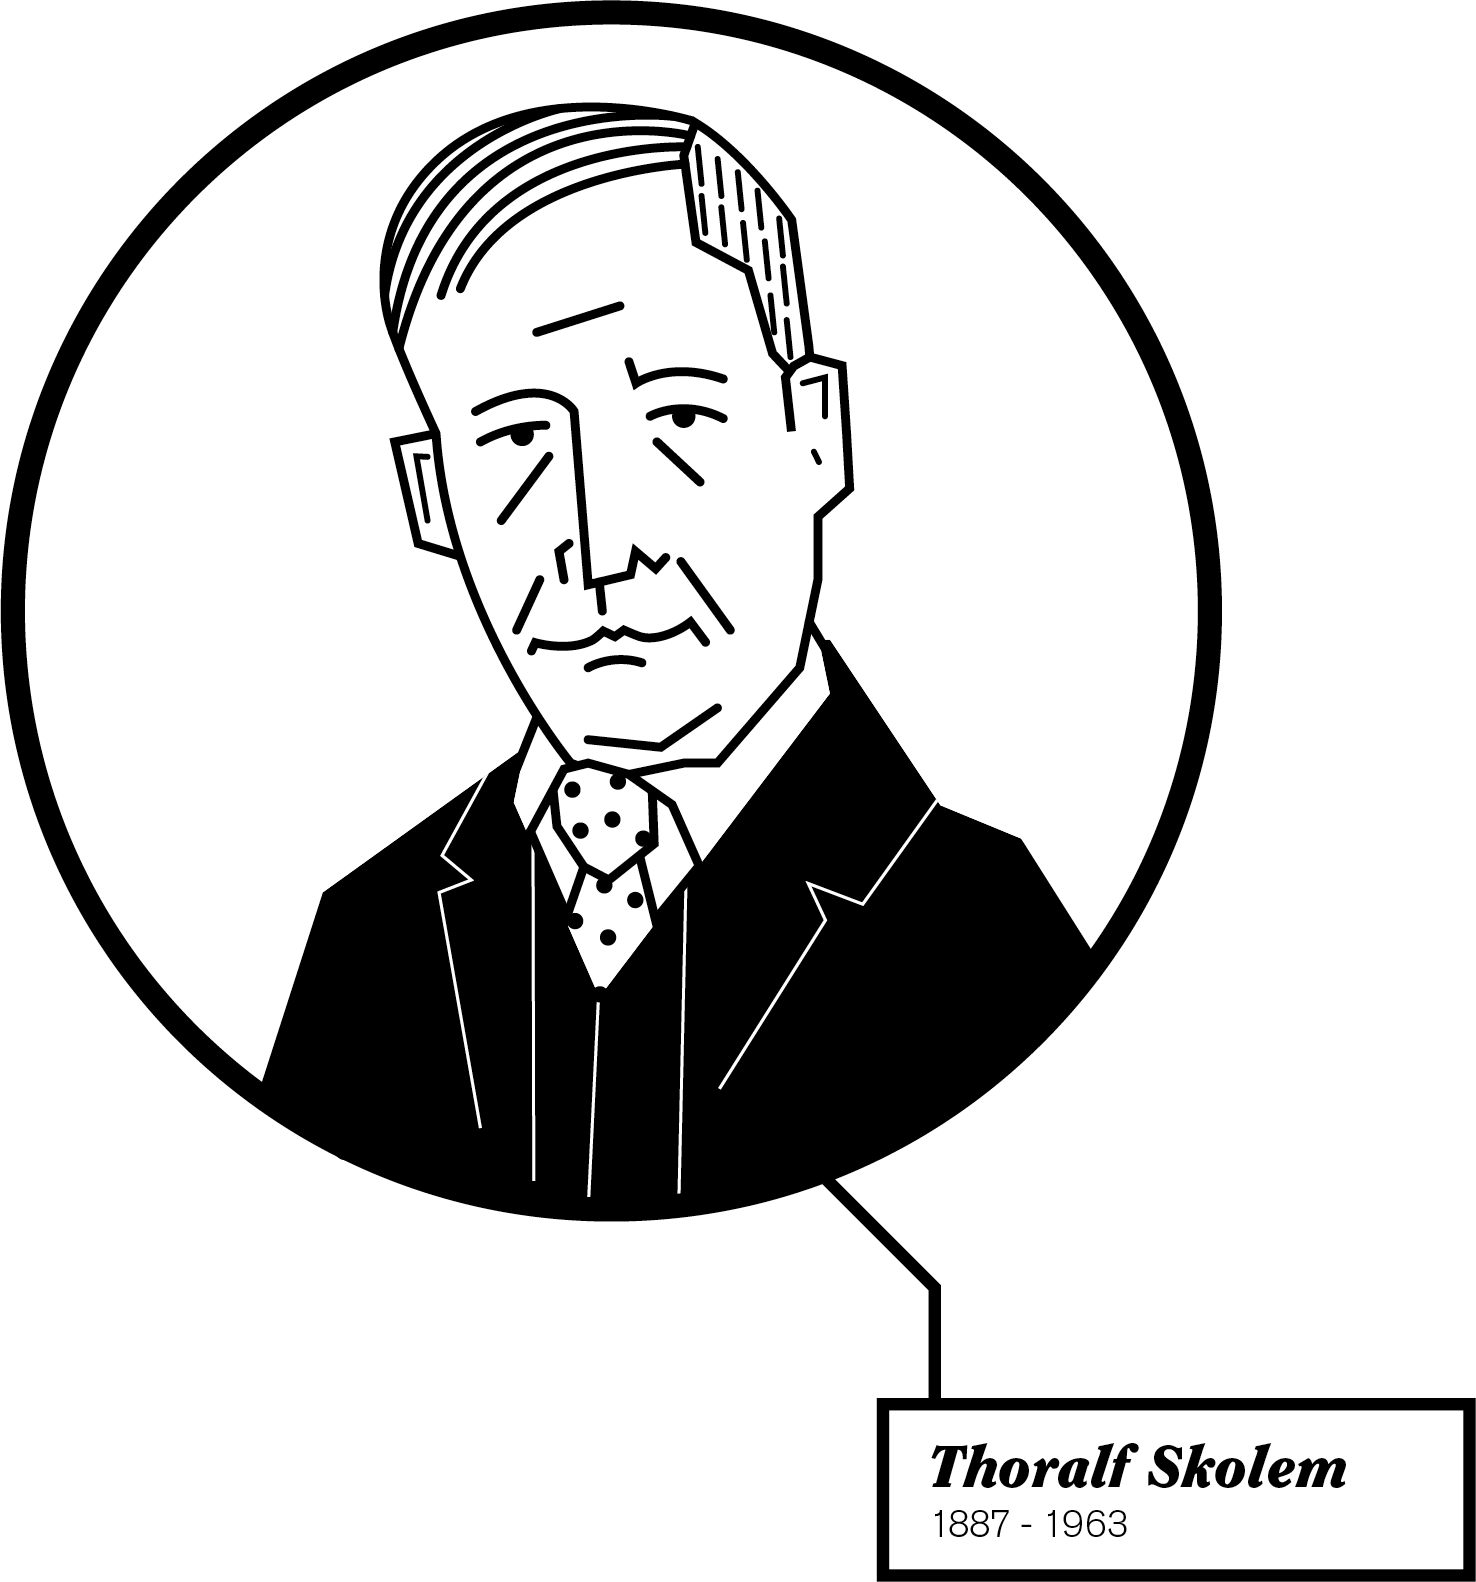
\includegraphics[width=\textwidth]{illustrations/SkolemChapter}
\vfill

\chapter{प्रस्तावना}

हे पुस्तक अधितर्कशास्त्राचा परिचय करून देते. ते विशेषतः संगणकशास्त्र आणि तत्त्वज्ञान यांच्या विद्यार्थ्यांसाठी आहे. तर्कशास्त्राचाच अभ्यास करणारी शाखा असल्यामुळे तिला ``अधितर्कशास्त्र'' असे नाव आहे. तर्कशास्त्रात वैध अनुमानाच्या नियमांचा विचार केला जातो. तर्कशास्त्राचे चिन्हात्मक किंवा आकारिक रूप हे नियम विधानीय किंवा प्रथम-क्रम तर्कशास्त्राच्या भाषांसारख्या आकारिक भाषांत मांडते. अधितर्कशास्त्रात या भाषांचे आणि त्या वापरून केलेल्या योग्य अनुमानाच्या नियमांचे गुणधर्म तपासले जातात. या आकारिक भाषांतील अभिव्यक्तींना नेमका अर्थ कसा द्यावा, वैध अनुमानाच्या नियमांचे समर्थन कसे करावे आणि विविध !!{derivation} पद्धतींचे गुणधर्म, त्यांच्या संगणनविषयक गुणधर्मांसह, कोणते आहेत, अशा प्रश्नांचा त्यात विचार होतो. येथे तपासलेल्या भाषा आणि !!{derivation} पद्धती अनेक क्षेत्रांत, विशेषतः गणित, तत्त्वज्ञान, संगणकशास्त्र आणि भाषाविज्ञान यांत वापरल्या जातात. त्यामुळे हे प्रश्न स्वतःच महत्त्वाचे आणि रंजक आहेत. शिवाय, सर्वसाधारणपणे आकारिक प्रणाल्यांचा अभ्यास कसा करावा हेही त्यांतून दिसते. येथे आपण ज्या तार्किक भाषा अभ्यासतो त्यांखेरीज इतरही भाषा अभ्यासकांच्या दृष्टीने महत्त्वाच्या आहेत. उदाहरणार्थ, भाषावैज्ञानिक आणि तत्त्वज्ञ यांना विधानीय व प्रथम-क्रम तर्कशास्त्राच्या भाषांपेक्षा कितीतरी गुंतागुंतीच्या भाषांत रस असतो. संगणकशास्त्रज्ञांना तर प्रोग्रामिंग भाषांसारख्या वेगळ्याच \emph{प्रकारच्या} भाषांत रस असतो. आकारिक भाषांची चिन्हार्थमीमांसा कशी द्यावी, त्यांच्याविषयीचे निष्कर्ष कसे सिद्ध करावेत आणि त्यांचे गुणधर्म कसे तपासावेत, यासाठी आपण पाहणार असलेल्या पद्धती तिथेही लागू होतात.

इतर कोणत्याही विद्याशाखेप्रमाणे अधितर्कशास्त्रातही निष्कर्ष किंवा तथ्ये आहेत आणि पद्धती व तंत्रेही आहेत. या पुस्तकात दोन्हींचा विचार केला आहे. पुष्कळ विद्यार्थ्यांना हा अभ्यासक्रम संपल्यावर आपण पाहिलेल्या प्रत्येक निष्कर्षाची गरज पडणार नाही, पण ते निष्कर्ष प्रस्थापित करण्यासाठी आपण ज्या पद्धती वापरतो त्यांची त्यांना गरज पडेल आणि ते त्या वापरतील. उदाहरणार्थ, लोव्हेनहाइम--स्कोलेम प्रमेय संगणकशास्त्रात वारंवार वापरले जात नाही, पण त्याच्या सिद्धतेसाठी आपण वापरतो त्या पद्धती तिथे वापरल्या जातात. याउलट, आपण पाहणार असलेले अनेक निष्कर्ष विज्ञानाचे तत्त्वज्ञान आणि सत्तामीमांसा यांतील काही वादांना लागू पडतात. तत्त्वज्ञानाच्या विद्यार्थ्यांना अभ्यासक्रमाबाहेर हे निष्कर्ष सिद्ध करता येण्याची गरज भासेलच असे नाही, पण त्यांचा आशय समजला पाहिजे. ते प्रस्थापित करण्यासाठी लागणाऱ्या व्याख्यांचा आणि सिद्धतांचा नीट विचार केला तरच हे निष्कर्ष खऱ्या अर्थाने \emph{समजतात}. या पुस्तकातील निष्कर्ष आणि पद्धती यांचा अभ्यास संगणकशास्त्र व तत्त्वज्ञान यांच्या विद्यार्थ्यांना सुचवला जातो, आणि काही अभ्यासक्रमांत तो आवश्यकही असतो, याची ही काही कारणे आहेत.

पुस्तकाचे तीन भाग आहेत. \Olref[sfr][][]{part} संचसिद्धान्ताविषयी आहे. तर्कशास्त्र व अधितर्कशास्त्र यांचा ``गणिताची पायाभरणी'' असे ज्याला म्हणतात त्याच्याशी ऐतिहासिकदृष्ट्या निकटचा संबंध आहे. पूर्णांक, परिमेय व वास्तव संख्या, फलने, अवकाश इत्यादी गणितीय वस्तू मुळात कशा समजून घ्याव्यात हा त्या अभ्यासाचा विषय आहे. संचसिद्धान्त त्याचे एक उत्तर देतो (इतरही उत्तरे आहेत). म्हणूनच संचसिद्धान्त आणि तर्कशास्त्र यांचा दीर्घकाळ एकत्र अभ्यास होत आला आहे. कोणत्याही प्रकारच्या आकारिक अभ्यासात संच, संबंध आणि फलने सर्वत्र आढळतात. गणिताबरोबरच संगणकशास्त्रात आणि तत्त्वज्ञानाच्या काही अधिक तांत्रिक शाखांतही ती दिसतात. तर्कशास्त्राची चिन्हार्थमीमांसा, सिद्धता उपपत्ती आणि संगणनक्षमतेची पायाभूत तत्त्वे यांविषयी निष्कर्ष मांडण्यासाठी व सिद्ध करण्यासाठी योग्य परिभाषा असणे आवश्यक आहे. उदाहरणार्थ, आपण अभिव्यक्तींचे संच, तार्किक निष्पन्नतेचे व सिद्धतायोग्यतेचे संबंध, विधेयचिन्हांचे अर्थनिर्धारण (त्यातून संबंधच मिळतात), संगणनक्षम फलने, त्यांच्यातील विविध संबंध आणि त्यांचा वापर करून केलेल्या विविध रचना यांविषयी बोलू. यासाठी संक्षिप्त संकेत असणे आणि संच, संबंध व फलने यांच्या सर्वसाधारण गुणधर्मांचा विचार करणे सोयीचे ठरेल. गणितीय विचार करण्याची आणि गणितीय सिद्धता मांडण्याची सवय नसेल, तर संचसिद्धान्ताचा पहिला भाग सरावाची संधी समजा. सर्व मूलभूत व्याख्या दिल्या जातील आणि त्यांचा वापर करून क्रमाक्रमाने अधिक गुंतागुंतीच्या सिद्धता दिल्या जातील. विशेषतः पहिल्या भागात, या सिद्धता समजून घेणे आणि त्या स्वतः शोधून मांडता येणे हे बहुधा निष्कर्ष समजून घेण्यापेक्षा अधिक महत्त्वाचे आहे. गणितीय विचार करण्याची तुम्हाला सवय नसेल, तर उदाहरणांचा आणि समस्यांचा नीट विचार करणे महत्त्वाचे आहे.

पहिल्या भागात मात्र आपण एक महत्त्वाचा निष्कर्ष प्रस्थापित करू. हा निष्कर्ष म्हणजे कँटरचे प्रमेय. विज्ञानात संकल्पनाविश्लेषणाची जी अत्यंत उल्लेखनीय उदाहरणे आढळतात त्यांपैकी एका उदाहरणावर तो आधारलेला आहे. ते म्हणजे कँटर यांनी केलेले अनंततेचे विश्लेषण. अनेक शतके गणितज्ञ आणि तत्त्वज्ञ दोघांनाही अनंततेने कोड्यात टाकले आहे. कँटर यांच्यापूर्वी तिचा नेमका विचार कसा करावा हे कोणालाच ठाऊक नव्हते. तिचा विचार करणे हीच चूक आहे आणि अनंत संग्रह ही कल्पनाच विसंगत आहे असेही पुष्कळांना वाटत असे. कँटर यांनी अनंततेचा सुसंगतपणे अभ्यास करणे शक्य केले. त्यांनी अनंत संग्रहांची आणि त्या संग्रहांचे आकारमान मोजता येईल अशा अनंत संख्यांची संपूर्ण उपपत्ती विकसित केली. अनंततेच्या वेगवेगळ्या पातळ्या आहेत हे त्यांनी दाखवले. ``अनंतपार'' संख्यांची ही उपपत्ती सुंदर आणि गुंतागुंतीची आहे. आपण तिच्यात फार खोलवर जाणार नाही, पण अनंततेच्या वेगवेगळ्या पातळ्या आहेत, विशेषतः ``गणनीय'' आणि ``अगणनीय'' पातळ्या आहेत, हे दाखवू शकू. या निष्कर्षाचे महत्त्वाचे उपयोग आहेत. शिवाय आपल्या विषयाची जाण ठेवू इच्छिणाऱ्या प्रत्येक गणितज्ञाला, संगणकशास्त्रज्ञाला आणि तत्त्वज्ञाला माहीत असावा असा हा निष्कर्ष आहे.

\olref[fol][][]{part} मध्ये आपण प्रथम-क्रम तर्कशास्त्राकडे वळतो. आपण प्रथम-क्रम तर्कशास्त्राची भाषा आणि तिची चिन्हार्थमीमांसा यांची व्याख्या करू. म्हणजेच प्रथम-क्रम रचना म्हणजे काय आणि प्रथम-क्रम तर्कशास्त्राचे वाक्य एखाद्या रचनेत केव्हा सत्य ठरते हे ठरवू. यामुळे आपल्याला दोन महत्त्वाच्या गोष्टी करता येतील. (1)~एखादे वाक्य दुसऱ्या वाक्यापासून तार्किकरीत्या केव्हा निष्पन्न होते हे गणितीय काटेकोरपणे सांगता येईल. (2)~प्रथम-क्रम रचनेतील संबंधांचे वर्णन, म्हणजेच त्यांचे लक्षणचित्रण, त्या रचनांमध्ये सत्य असणारी वाक्ये कशा रीतीने करतात हे पाहता येईल. यातून विशेषतः स्वयंसिद्धकीय पद्धतीची चर्चा पुढे येते. या पद्धतीत विशिष्ट प्रकारच्या रचनांचे लक्षणचित्रण करण्यासाठी प्रथम-क्रम भाषांतील वाक्ये वापरली जातात. पुढे आपण सिद्धता उपपत्ती पाहू. त्यात गरहार्ड गेंटझेन यांनी १९३० च्या दशकात परिभाषित केलेली क्रमवर्ती कलनाची आणि नैसर्गिक निगमनाची मूळ रूपे पाहू. (तुमचे अध्यापक यांपैकी एकच पद्धत शिकवण्याचे ठरवू शकतात. तसे झाल्यास ``!!{derivation}s'' आणि ``!!{derivability}'' यांचा उल्लेख त्यांनी निवडलेल्या पद्धतीच्या संदर्भात समजावा.) एखादे वाक्य इतर काही वाक्यांवरून निष्पन्न होते ही कल्पना नेमकी करण्याचे दोन सर्वस्वी वेगळे मार्ग आपल्याला मिळतात. एक म्हणजे तार्किक निष्पन्नतेची चिन्हार्थविषयक संकल्पना आणि दुसरा म्हणजे !!{derivability} ची विन्यासात्मक संकल्पना. निर्दोषता आणि संपूर्णता ही प्रमेये या दोन लक्षणचित्रणांचा संबंध जोडतात. विशेषतः आपण गोडेल यांचे संपूर्णता प्रमेय सिद्ध करू. त्यानुसार एखादे वाक्य इतर काही वाक्यांपासून चिन्हार्थाच्या दृष्टीने निष्पन्न होत असेल, तर ते त्यांच्यापासून !!{derivable} ही असते. याची समतुल्य मांडणी अशी आहे. एखादा वाक्यसंच सुसंगत असेल, म्हणजे त्यावरून व्याघात सिद्ध करता येत नसेल, तर ती सर्व वाक्ये सत्य ठरतील अशी एखादी रचना असते.

संपूर्णता प्रमेयाची दुसरी मांडणी कदाचित अधिक आश्चर्यकारक आहे. गोडेल यांनी हा निष्कर्ष सिद्ध केला त्या सुमारास (१९२९ मध्ये) डाव्हीट हिल्बर्ट या जर्मन गणितज्ञाचे एक प्रसिद्ध मत असे होते की गणितीय अस्तित्वासाठी सुसंगतता, म्हणजे व्याघाताचा अभाव, एवढीच अट पुरेशी आहे. दुसऱ्या शब्दांत, एखाद्या रचनेचे किंवा रचनांच्या वर्गाचे सुसंगत वर्णन एखाद्या गणितज्ञाला करता येत असेल, तर अशा रचना अस्तित्वात आहेत असे मानण्याचा त्याला अधिकार असावा. त्या काळात अनेकांना ही कल्पना हास्यास्पद वाटली. एखाद्या रचनेचे वर्णन करताना आपण स्वतःशी विसंगत बोललो नाही, एवढ्यावरून ती रचना खरोखर अस्तित्वात आहे असा निष्कर्ष कसा निघणार? गोडेल यांचे संपूर्णता प्रमेय नेमके हेच सांगते. विरोधापत्तीसारख्या आणि तत्त्वज्ञानाच्या दृष्टीने कुतूहलजनक अशा या पैलूबरोबरच संपूर्णता प्रमेयाचे दोन महत्त्वाचे उपयोगही आहेत. दिलेली वाक्ये सत्य ठरवणाऱ्या रचनांच्या अस्तित्वाविषयी आणखी निष्कर्ष सिद्ध करण्यासाठी ते उपयोगी पडतात. हे निष्कर्ष म्हणजे संहतता प्रमेय आणि लोव्हेनहाइम--स्कोलेम प्रमेय.

\olref[tur][][]{part} मध्ये आपण तर्कशास्त्राचा संबंध संगणनक्षमतेशी जोडतो. यालाही ऐतिहासिक संदर्भ आहे. तर्कशास्त्रातील एखादे दिलेले वाक्य सिद्ध करता येते की नाही हे ठरवणारी यांत्रिक पद्धत शोधणे ही तर्कशास्त्राची एक मूलभूत समस्या म्हणून डाव्हीट हिल्बर्ट यांनी मांडली होती. विधानीय तर्कशास्त्रासाठी अशी पद्धत अर्थातच आहे. सर्व सत्यताकोष्टके तपासली की झाले. ती सांत संख्येने असल्यामुळे या पद्धतीने अखेरीस योग्य उत्तर मिळते. प्रथम-क्रम तर्कशास्त्रासाठी इतकी सरळ पद्धत शक्य नाही, कारण संभाव्य रचना अनंत संख्येने असतात (आणि रचना स्वतःही अनंत असू शकतात). अधिक कल्पक पद्धत शोधण्यासाठी तर्कशास्त्रज्ञ अनेक वर्षे प्रयत्न करत होते. ॲलोन्झो चर्च आणि ॲलन ट्यूरिंग यांनी अखेरीस अशी कोणतीही पद्धत अस्तित्वात नसल्याचे सिद्ध केले. त्यासाठी सर्वसाधारणपणे यांत्रिक पद्धत म्हणजे काय याची प्रथम नेमकी व्याख्या देणे आवश्यक होते. एखादी निर्णयप्रक्रिया सुचवली गेली असती, तर बहुधा ती प्रभावी पद्धत आहे हे ओळखता आले असते. पण कोणतीही प्रभावी पद्धत अस्तित्वात नाही हे सिद्ध करण्यासाठी ``प्रभावी पद्धत'' याची आधी व्याख्या करावी लागते आणि त्या व्याख्येच्या आधारे अशक्यता सिद्ध करावी लागते. ट्यूरिंग यांनी हेच केले. तत्त्वतः एखाद्या यांत्रिक प्रक्रियेला काय करता येते याचे गणितीय प्रतिमान म्हणून त्यांनी ट्यूरिंग यंत्राची\footnote{अर्थात, ट्यूरिंग यांनी स्वतः त्याला हे नाव दिले नव्हते.} कल्पना मांडली. गणितीय साधनांनी एखाद्या अनौपचारिक संकल्पनेचे \emph{संकल्पनाविश्लेषण} करण्याचे हे आणखी एक उदाहरण आहे. कँटर यांचे अनंततेचे विश्लेषण गणिताला जितके महत्त्वाचे आहे, तितकेच हे विश्लेषण संगणकशास्त्राला कदाचित महत्त्वाचे आहे. शेवटचे मोठे काम म्हणजे अशक्यतेची दोन प्रमेये सिद्ध करणे. ``थांबण्याची समस्या'' म्हणून ओळखली जाणारी समस्या ट्यूरिंग यंत्रांना सोडवता येत नाही हे आपण दाखवू. शेवटी, तर्कशास्त्रासाठी हिल्बर्ट यांनी मांडलेली ``निर्णय समस्या''ही त्यांना सोडवता येत नाही हे दाखवू.

हे पुस्तक गणितीय आहे, कारण त्यात आपण गणितीय व्याख्यांची चर्चा करतो आणि आपले निष्कर्ष गणितीय रीतीने सिद्ध करतो. मात्र त्यासाठी गणिताचे विस्तृत पूर्वज्ञान आवश्यक नाही. पुस्तकातील कोणत्याही भागासाठी बीजगणित, त्रिकोणमिती किंवा कलन यांचे ज्ञान लागत नाही. गणितात काम कसे केले जाते याचाही आधीचा परिचय लागणार नाही याची आम्ही विशेष काळजी घेतली आहे. खरे तर, आपले निष्कर्ष समजून घेण्यासाठी आणि सिद्ध करण्यासाठी लागणारे युक्तिविचार आणि सिद्धता देण्याचे कौशल्य \emph{विकसित करणे} हा या पुस्तकाच्या हेतूचा एक भाग आहे. पुस्तकाची मांडणी गणितातील संकेतांनुसार आहे. गणितात स्पष्टता आणि काटेकोरपणा यांना विशेष महत्त्व असल्यामुळे हे संकेत विकसित झाले आहेत. उदाहरणार्थ, एखादी गोष्ट युक्तिवादाचा निष्कर्ष म्हणून मांडली आहे, दुसऱ्या गोष्टीच्या समर्थनार्थ दिली आहे की नव्या संज्ञेची ओळख करून देण्यासाठी आली आहे, हे समजणे आवश्यक असते. म्हणून आपण गणितातील संकेत पाळतो. नवीन संज्ञा किंवा चिन्हे देणाऱ्या मजकुराला ``व्याख्या'' असे म्हणतो आणि निष्कर्ष किंवा एखादी सिद्ध झालेली बाब नोंदवताना ``प्रमेय'', ``विधान'', ``पूर्वप्रमेय'' किंवा ``अनुप्रमेय'' असे म्हणतो. या संकेतांबरोबरच तर्कशास्त्राच्या पहिल्या अभ्यासक्रमातून कदाचित परिचित असलेल्या तार्किक सिद्धतेच्या पद्धती आपण वापरू. निष्कर्ष सिद्ध करण्यासाठी \emph{विगमन} पद्धतीचाही भरपूर वापर करू. परिशिष्टाची दोन प्रकरणे या सिद्धता-पद्धतींना वाहिलेली आहेत.

\paragraph{अध्यापकांसाठी सूचना} या पुस्तकातील सामग्री आकारिक तर्कशास्त्राच्या दुसऱ्या, एका सत्राच्या अभ्यासक्रमासाठी योग्य आहे. कॅलगरी विद्यापीठात मी तर्कशास्त्र~II या अभ्यासक्रमात ती १२ आठवड्यांत शिकवतो. मात्र पुस्तकात दिले आहे तितक्या तपशिलात सर्व विषय शिकवत नाही. उदाहरणार्थ, मी सामान्यतः फक्त नैसर्गिक निगमन शिकवतो आणि एकरूपतेसाठी संपूर्णतेच्या तपशीलवार सिद्धता वगळतो. विद्यार्थ्यांनी त्याआधी तर्कशास्त्र~I हा अभ्यासक्रम घेतलेला असतो. तो सहसा \emph{\href{https://forallx.openlogicproject.org}{forall x: Calgary}} या पुस्तकावरून शिकवला जातो. त्यात नैसर्गिक निगमनाचे हेच नियम वापरले आहेत, पण फिच यांच्या मांडणीत.

या पुस्तकाची सर्वांत अलीकडची PDF आवृत्ती \href{https://slc.openlogicproject.org}{मूळ पाठ्यपुस्तकाच्या संकेतस्थळावर} उपलब्ध आहे, पण ती वारंवार बदलते. CC BY परवान्यामुळे तुम्हाला स्वतः पुस्तक डाउनलोड करून वितरित करण्याचा अधिकार मिळतो.\footnote{CC BY 4.0 हा मजकुराचा परवाना आहे. या मराठी PDF मधील व्यक्तिचित्रे व छायाचित्रे वितरित करताना त्यांच्या स्वतंत्र वापराच्या अटी लागू होतात. त्या पुस्तकाच्या श्रेयपृष्ठांवर दिल्या आहेत.} तुम्ही ते वापरत असलेल्या संपूर्ण सत्रात सर्व विद्यार्थ्यांकडे एकच आवृत्ती असावी यासाठी या अधिकाराचा उपयोग करा. तुम्ही वापरायचे ठरवलेले PDF आपल्या शिक्षण व्यवस्थापन प्रणालीवर अपलोड करा. विद्यार्थ्यांना केवळ दुवा दिल्यास ते एकाच आवृत्तीचा वापर करतील याची खात्री राहत नाही. तुमच्या पुस्तकविक्रेत्याकडून तुम्ही PDF छापून घेऊ शकता. काही पुस्तकविक्रेत्यांना Amazon वर उपलब्ध असलेल्या मऊ मुखपृष्ठाच्या प्रती विकत घेऊन विक्रीसाठी ठेवता येतील.

ग्रॅहम लीच-क्राउस यांचे विनामूल्य ऑनलाइन तर्कशास्त्र अध्यापन साधन \emph{Carnap} (\href{https://carnap.io}{carnap.io}) प्रथम-क्रम तर्कशास्त्राची विन्यासमीमांसा, चिन्हार्थमीमांसा आणि सिद्धता-पद्धती यांच्या अभ्यासाला पूरक आहे. नैसर्गिक निगमन व क्रमवर्ती कलनातील !!{derivation}s, साध्या उपपत्तींसाठी रचना देणे आणि चिन्हांकन यांसारख्या सरावांची उत्तरे त्यात सादर करता येतात आणि त्यांचे स्वयंचलित मूल्यमापन होते. \href{https://turing.openlogicproject.org}{turing.openlogicproject.org} येथे ट्यूरिंग यंत्राचे अनुकरण करणारे साधनही आहे. \olref[tur][][]{part} मधील सामग्री उदाहरणांसह समजावण्यासाठी ते वापरता येते. तिथली उदाहरणे या साधनात आधीच भरलेली आहेत.

\cleartoverso

\thispagestyle{empty}
\ \vfill
\noindent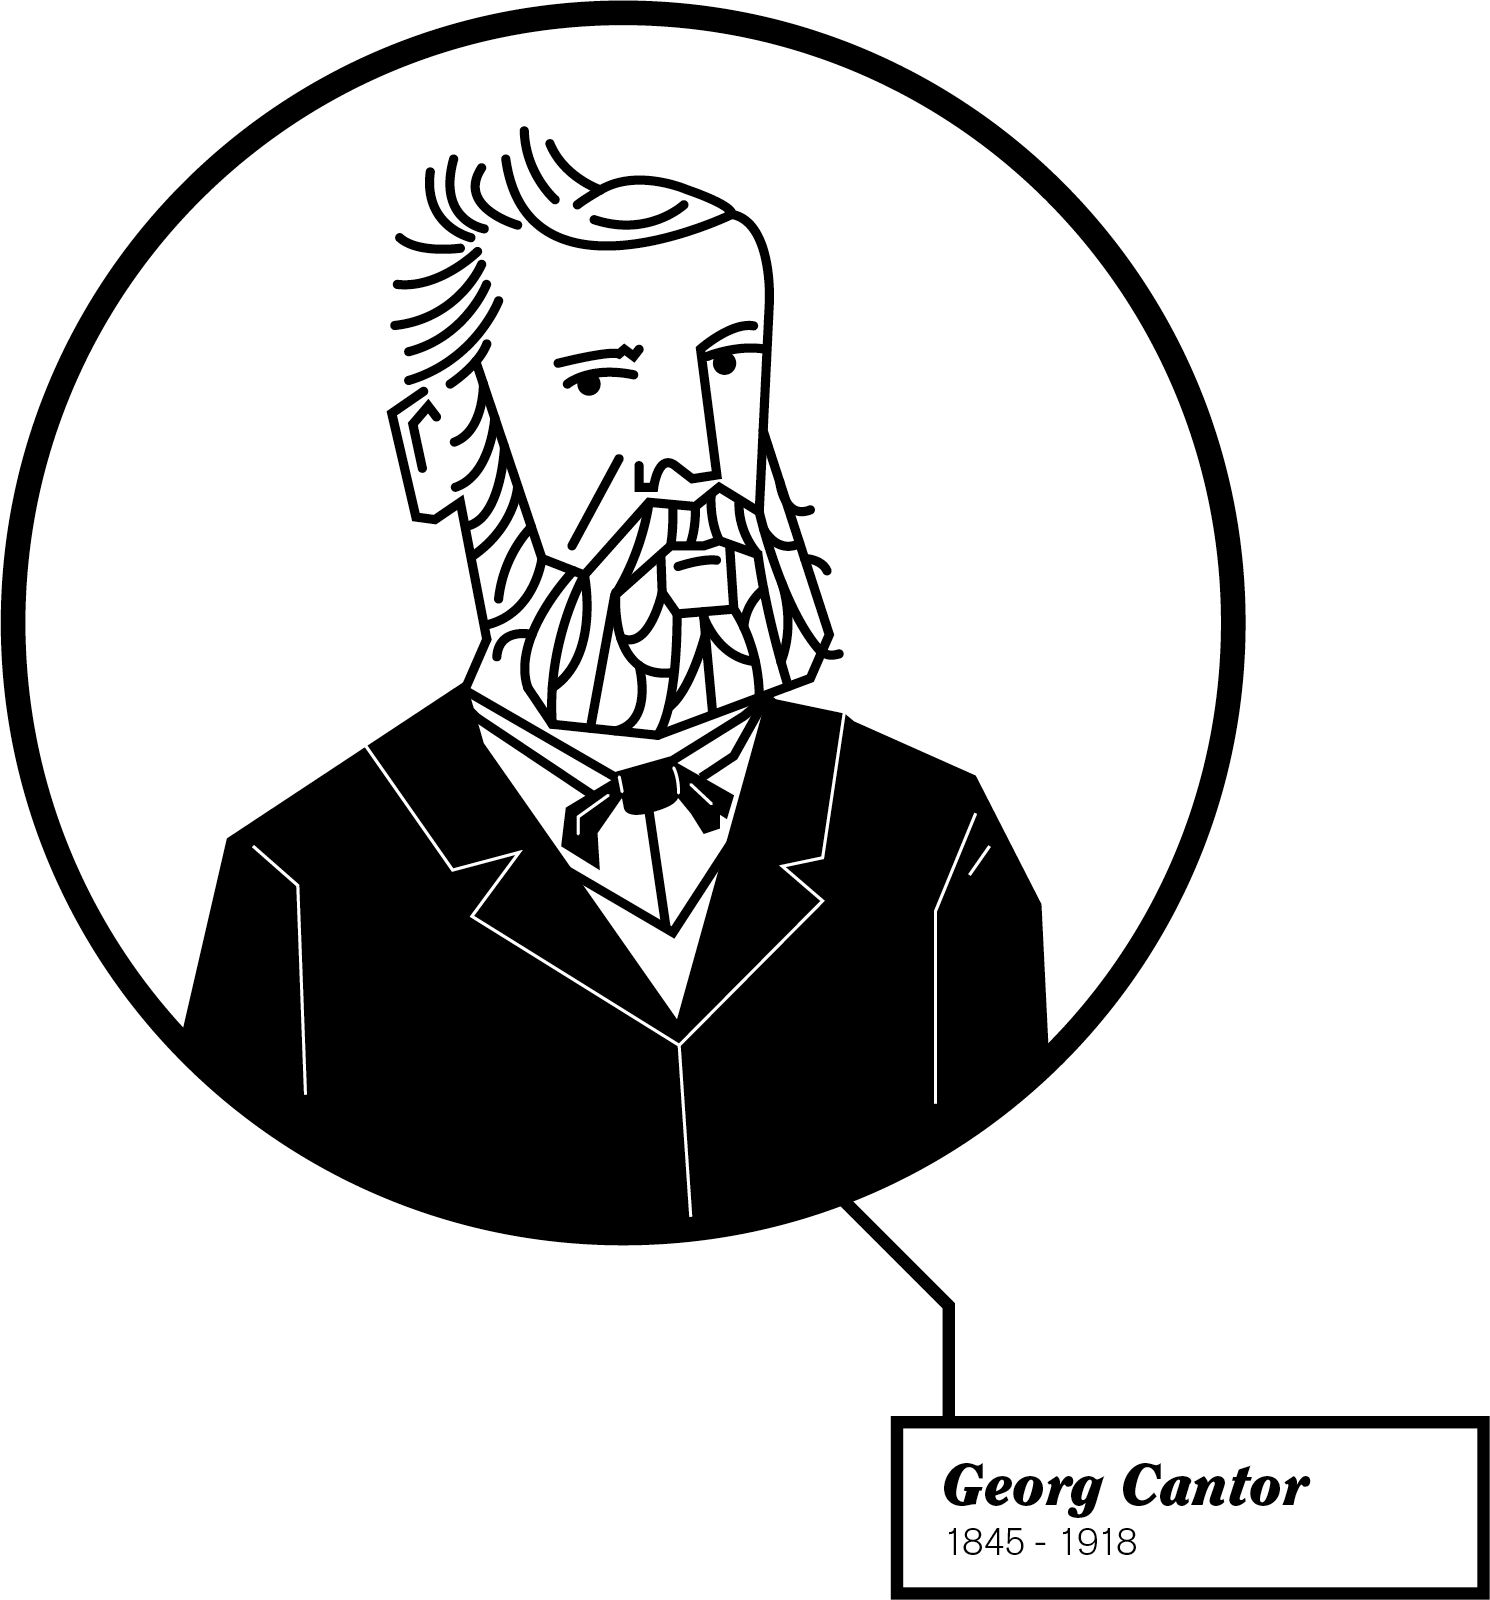
\includegraphics[width=\textwidth]{illustrations/CantorChapter}
\vfill

\mainmatter

\olimport*[sets-functions-relations]{sets-functions-relations}
\cleartoverso
\ifodd\value{page}\stepcounter{page}\fi
\thispagestyle{empty}
\ \vfill
\noindent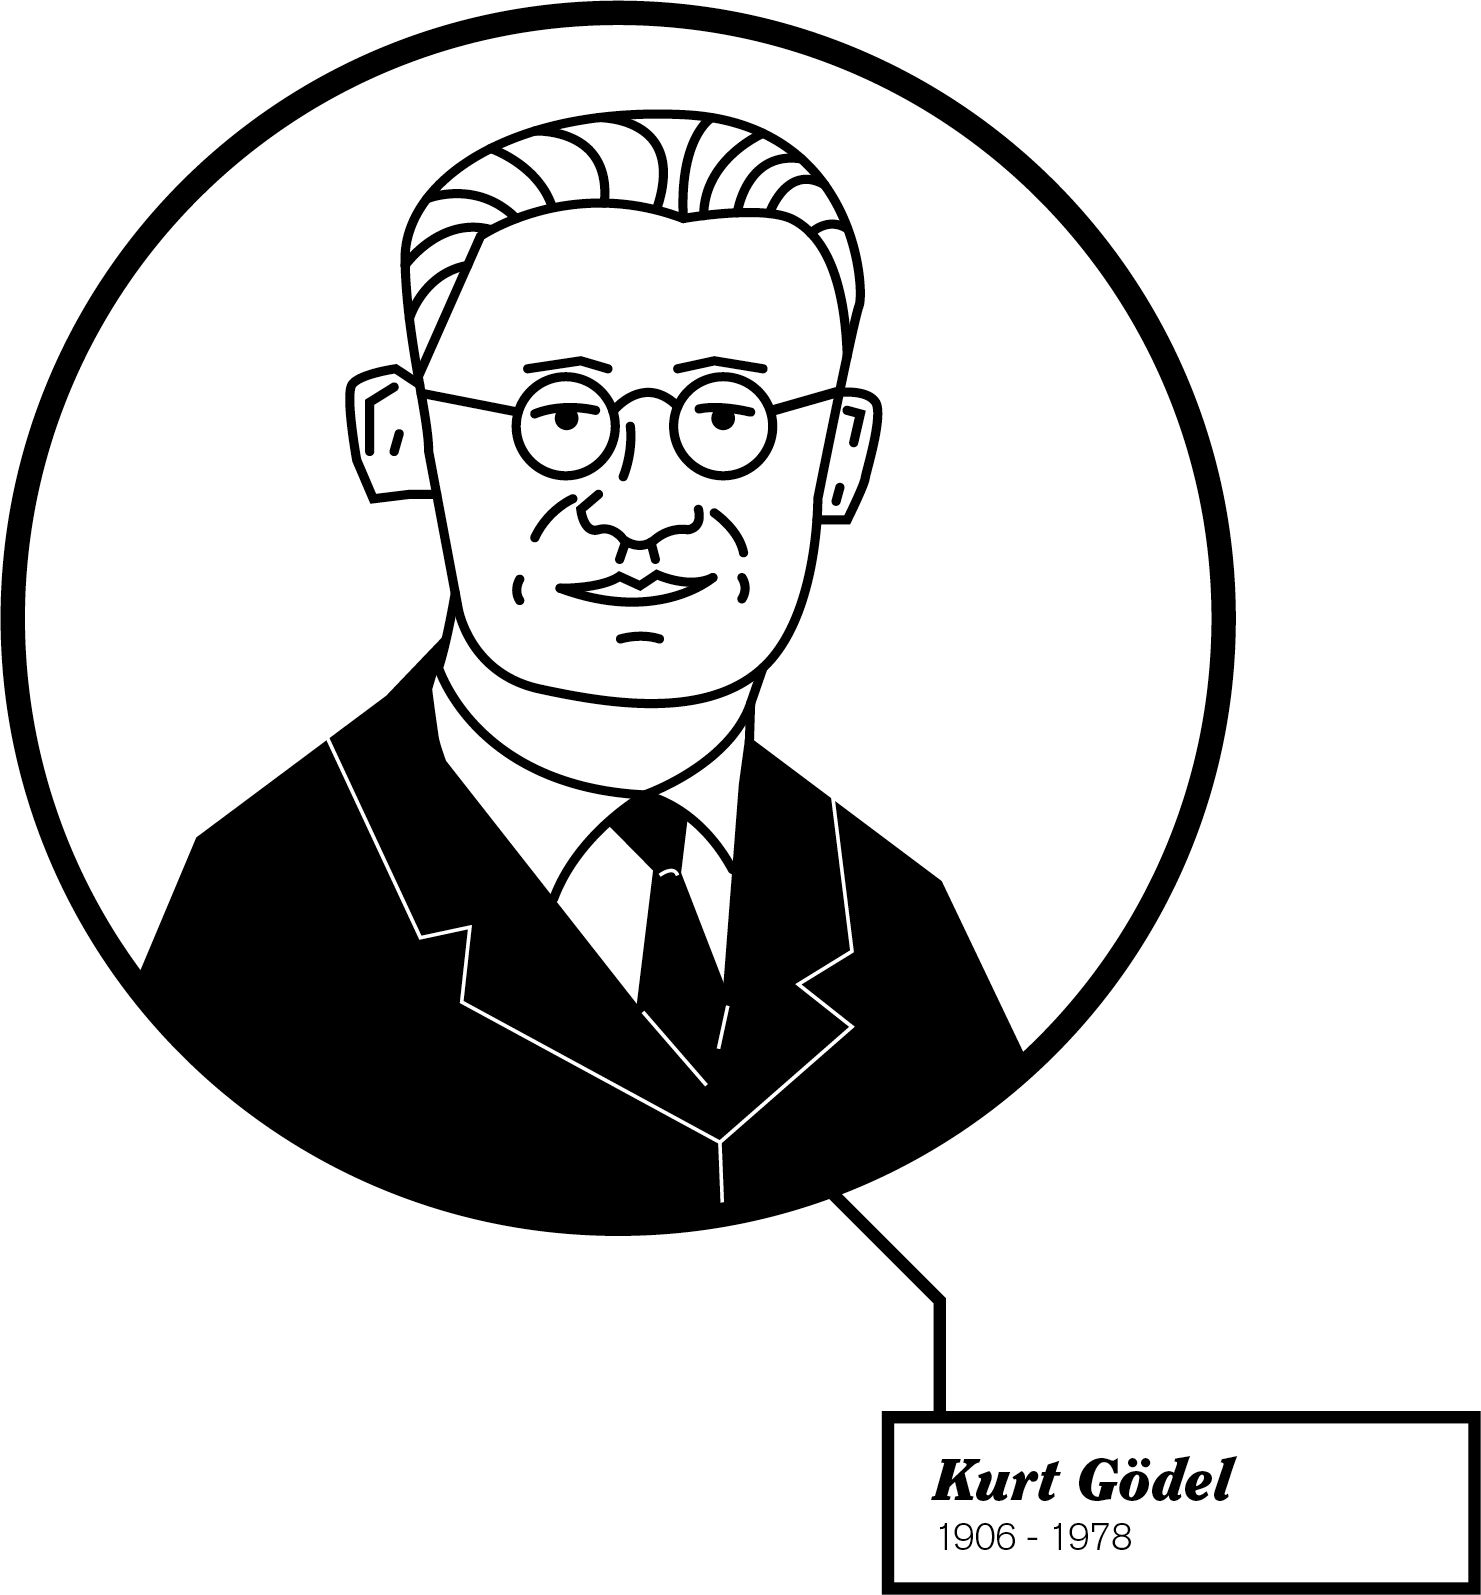
\includegraphics[width=\textwidth]{illustrations/GodelChapter}
\vfill

\olimport*[first-order-logic]{first-order-logic}
\cleartoverso
\ifodd\value{page}\stepcounter{page}\fi
\thispagestyle{empty}
\ \vfill
\noindent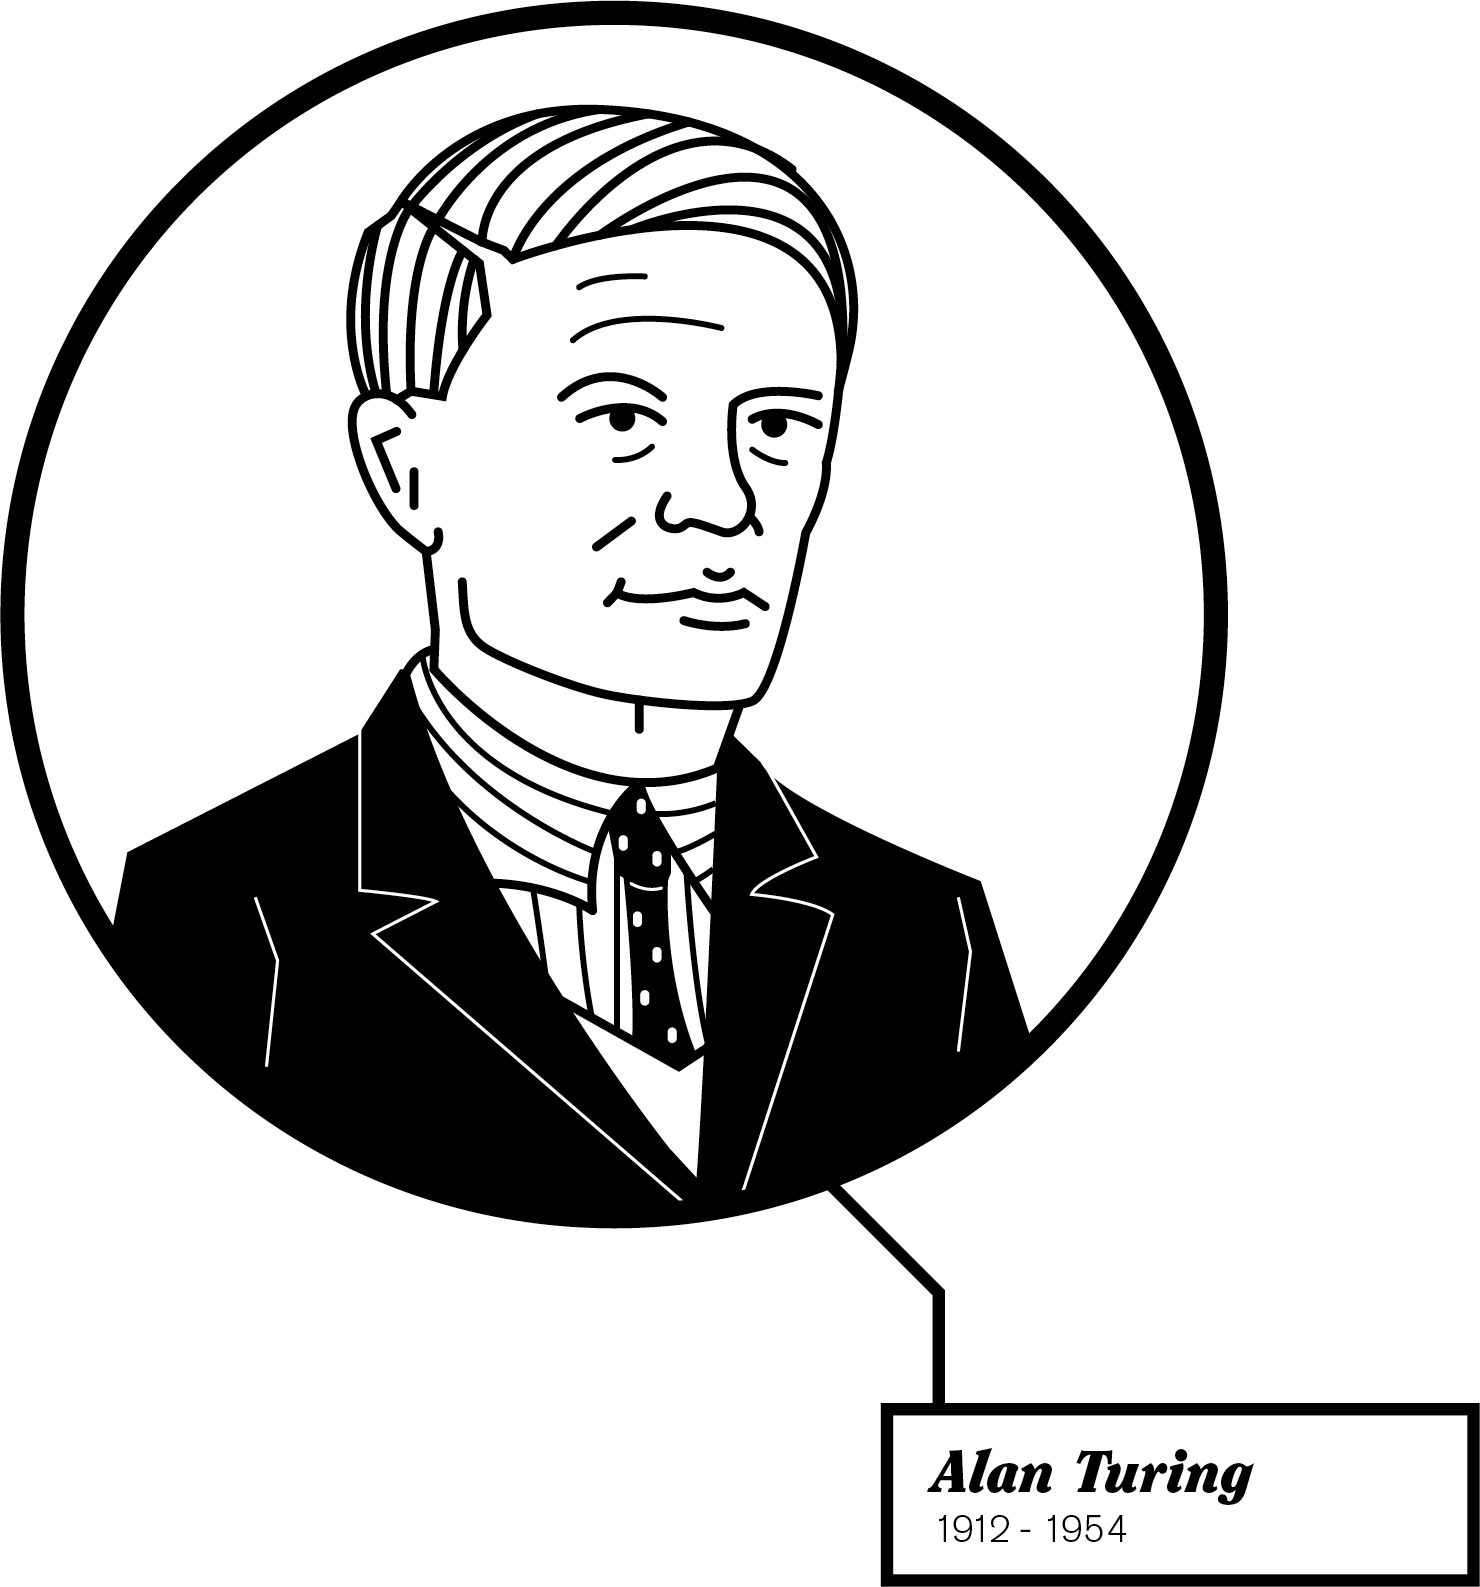
\includegraphics[width=\textwidth]{illustrations/TuringChapter}
\vfill

\olimport*[turing-machines]{turing-machines}

\cleartoverso
\ifodd\value{page}\stepcounter{page}\fi
\thispagestyle{empty}
\ \vfill
\noindent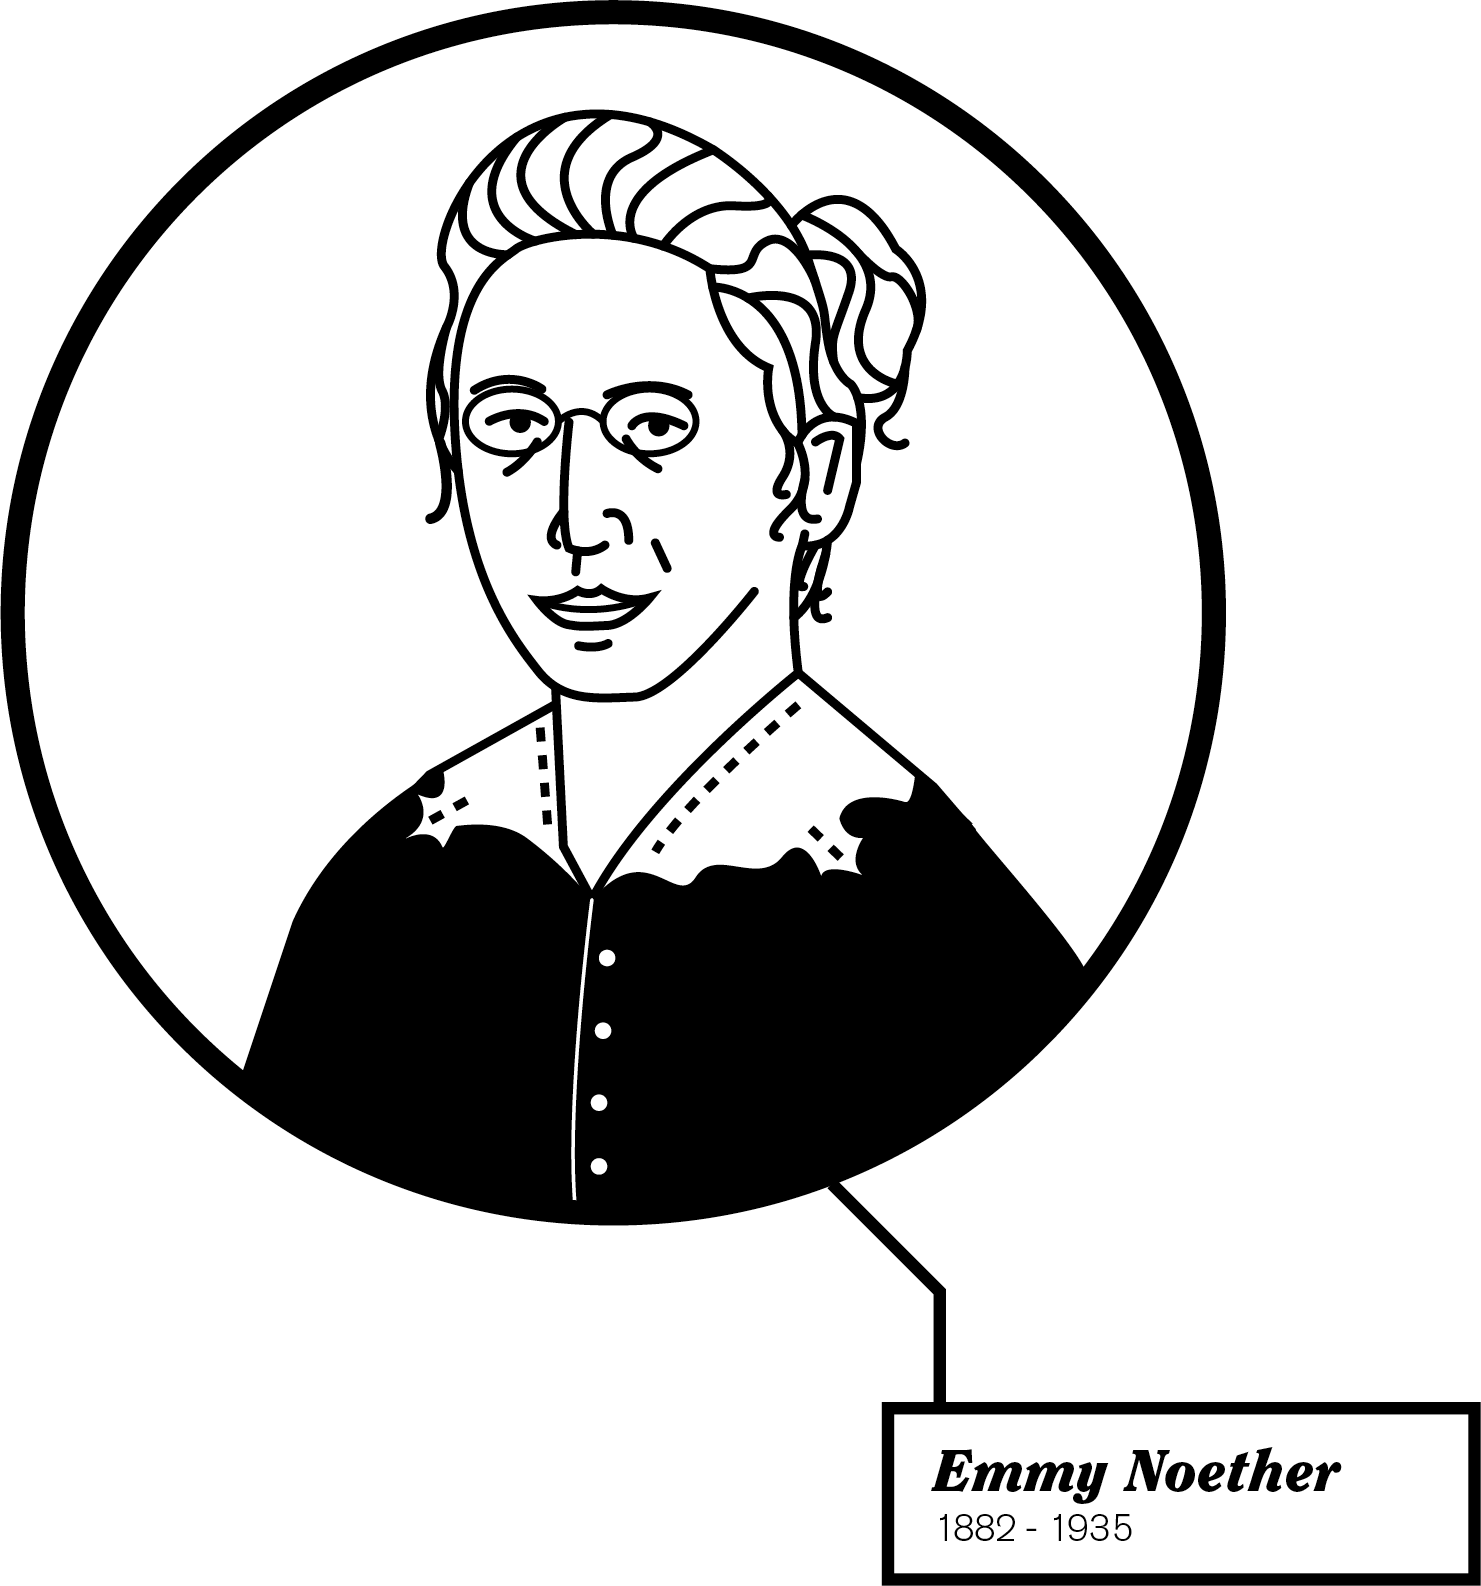
\includegraphics[width=\textwidth]{illustrations/NoetherChapter}
\vfill

% The SLC summary files belong to the numbered chapters.
\slcChapterSummariesfalse
\appendix

\olimport*[methods/proofs]{proofs}

\olimport*[methods/induction]{induction}

\stopproblems
\def\ifproblems#1{}

\setlength{\olphotowidth}{.45\textwidth}

\chapter{चरित्रे}

\olimport*[history/biographies]{georg-cantor}
\olimport*[history/biographies]{alonzo-church}
\olimport*[history/biographies]{gerhard-gentzen}
\olimport*[history/biographies]{kurt-goedel}
\olimport*[history/biographies]{emmy-noether}
\olimport*[history/biographies]{bertrand-russell}
\olimport*[history/biographies]{alfred-tarski}
\olimport*[history/biographies]{alan-turing}
\olimport*[history/biographies]{ernst-zermelo}
\olimport*[reference/greek-alphabet]{greek-alphabet}

\glsaddall
\printglossary[style=index,title=शब्दसूची,toctitle=शब्दसूची]

\clearpage
\photocredits

\bibliographystyle{natbib-oup}
\bibliography{\olpath/bib/open-logic}

{% The two-line Marathi heading leaves less room for the About text.
\addtolength{\beforechapskip}{-\baselineskip}%
\addtolength{\afterchapskip}{-\baselineskip}%
\olimport*{\olpath/locale/\ollangid/content/open-logic-about}\par}
\end{filecontents*}

\begin{filecontents*}{slc-config.sty}
% Mathematical and exercise choices of the source SLC textbook.
\ollatinformulas
\DeclareMathAlphabet{\mathbi}{OT1}{pplx}{b}{it}
\DeclareDocumentCommand\Struct{m}{\applytofirst{\mathbi}{#1}}
\DeclareDocumentMacro\TMblank{\sqcup}
\DeclareDocumentMacro\TMstroke{I}

\tagtrue{defIff,defTrue}
\tagfalse{prvIff,prvTrue}
\tagtrue{probAnd,probIf,probAll}
\tagtrue{prfND,prfSC}
\tagfalse{prfAX,prfTab}

% Sets, Logic, Computation uses “countable” for “enumerable”.
\mrsettexttoken{enumerable}{गणनीय}{गणनीय}
\mrsettexttoken{nonenumerable}{अगणनीय}{अगणनीय}
\mrsettexttoken{denumerable}{गणनीय अनंत}{गणनीय अनंत}

% Use the glossary terms for the syntactic relation and preserve semantic
% consequence as तार्किक निष्पन्नता.
\mrsettexttoken{derivable}{सिद्धतायोग्य}{सिद्धतायोग्य}
\mrsettexttoken{derivability}{सिद्धतायोग्यता}{सिद्धतायोग्यता}
\mrsettexttoken{nonderivability}{सिद्धतायोग्यतेचा अभाव}{सिद्धतायोग्यतेचा अभाव}
\mrsettexttoken{provable}{सिद्धतायोग्य}{सिद्धतायोग्य}
\mrsettexttoken{provability}{सिद्धतायोग्यता}{सिद्धतायोग्यता}
\mrsettexttoken{nonprovability}{सिद्धतायोग्यतेचा अभाव}{सिद्धतायोग्यतेचा अभाव}


\end{filecontents*}

\begin{filecontents*}{slc-envs.sty}
\usepackage{\olpath/sty/open-logic-book-envs}
\end{filecontents*}

\begin{filecontents*}{slc-screen.xmpdata}
\Title{संच, तर्कशास्त्र, संगणन — अधितर्कशास्त्राची मुक्त ओळख}
\Author{Richard Zach\sep Open Logic Project}
\Language{mr-Deva-IN}
\Keywords{तर्कशास्त्र\sep प्रथम-क्रम तर्कशास्त्र\sep संचसिद्धान्त\sep ट्यूरिंग यंत्रे}
\Copyright{मजकूर CC BY 4.0. रेखाचित्रे CC BY-NC 4.0. छायाचित्रांच्या स्वतंत्र अटी पुस्तकात दिल्या आहेत.}
\PublicationType{book}
\URLlink{https://slc.openlogicproject.org/}
\end{filecontents*}

\begin{filecontents*}{include/preface.tex}
\chapter{प्रस्तावना}

हे पुस्तक अधितर्कशास्त्राचा परिचय करून देते. ते विशेषतः संगणकशास्त्र आणि तत्त्वज्ञान यांच्या विद्यार्थ्यांसाठी आहे. तर्कशास्त्राचाच अभ्यास करणारी शाखा असल्यामुळे तिला ``अधितर्कशास्त्र'' असे नाव आहे. तर्कशास्त्रात वैध अनुमानाच्या नियमांचा विचार केला जातो. तर्कशास्त्राचे चिन्हात्मक किंवा आकारिक रूप हे नियम विधानीय किंवा प्रथम-क्रम तर्कशास्त्राच्या भाषांसारख्या आकारिक भाषांत मांडते. अधितर्कशास्त्रात या भाषांचे आणि त्या वापरून केलेल्या योग्य अनुमानाच्या नियमांचे गुणधर्म तपासले जातात. या आकारिक भाषांतील अभिव्यक्तींना नेमका अर्थ कसा द्यावा, वैध अनुमानाच्या नियमांचे समर्थन कसे करावे आणि विविध !!{derivation} पद्धतींचे गुणधर्म, त्यांच्या संगणनविषयक गुणधर्मांसह, कोणते आहेत, अशा प्रश्नांचा त्यात विचार होतो. येथे तपासलेल्या भाषा आणि !!{derivation} पद्धती अनेक क्षेत्रांत, विशेषतः गणित, तत्त्वज्ञान, संगणकशास्त्र आणि भाषाविज्ञान यांत वापरल्या जातात. त्यामुळे हे प्रश्न स्वतःच महत्त्वाचे आणि रंजक आहेत. शिवाय, सर्वसाधारणपणे आकारिक प्रणाल्यांचा अभ्यास कसा करावा हेही त्यांतून दिसते. येथे आपण ज्या तार्किक भाषा अभ्यासतो त्यांखेरीज इतरही भाषा अभ्यासकांच्या दृष्टीने महत्त्वाच्या आहेत. उदाहरणार्थ, भाषावैज्ञानिक आणि तत्त्वज्ञ यांना विधानीय व प्रथम-क्रम तर्कशास्त्राच्या भाषांपेक्षा कितीतरी गुंतागुंतीच्या भाषांत रस असतो. संगणकशास्त्रज्ञांना तर प्रोग्रामिंग भाषांसारख्या वेगळ्याच \emph{प्रकारच्या} भाषांत रस असतो. आकारिक भाषांची चिन्हार्थमीमांसा कशी द्यावी, त्यांच्याविषयीचे निष्कर्ष कसे सिद्ध करावेत आणि त्यांचे गुणधर्म कसे तपासावेत, यासाठी आपण पाहणार असलेल्या पद्धती तिथेही लागू होतात.

इतर कोणत्याही विद्याशाखेप्रमाणे अधितर्कशास्त्रातही निष्कर्ष किंवा तथ्ये आहेत आणि पद्धती व तंत्रेही आहेत. या पुस्तकात दोन्हींचा विचार केला आहे. पुष्कळ विद्यार्थ्यांना हा अभ्यासक्रम संपल्यावर आपण पाहिलेल्या प्रत्येक निष्कर्षाची गरज पडणार नाही, पण ते निष्कर्ष प्रस्थापित करण्यासाठी आपण ज्या पद्धती वापरतो त्यांची त्यांना गरज पडेल आणि ते त्या वापरतील. उदाहरणार्थ, लोव्हेनहाइम--स्कोलेम प्रमेय संगणकशास्त्रात वारंवार वापरले जात नाही, पण त्याच्या सिद्धतेसाठी आपण वापरतो त्या पद्धती तिथे वापरल्या जातात. याउलट, आपण पाहणार असलेले अनेक निष्कर्ष विज्ञानाचे तत्त्वज्ञान आणि सत्तामीमांसा यांतील काही वादांना लागू पडतात. तत्त्वज्ञानाच्या विद्यार्थ्यांना अभ्यासक्रमाबाहेर हे निष्कर्ष सिद्ध करता येण्याची गरज भासेलच असे नाही, पण त्यांचा आशय समजला पाहिजे. ते प्रस्थापित करण्यासाठी लागणाऱ्या व्याख्यांचा आणि सिद्धतांचा नीट विचार केला तरच हे निष्कर्ष खऱ्या अर्थाने \emph{समजतात}. या पुस्तकातील निष्कर्ष आणि पद्धती यांचा अभ्यास संगणकशास्त्र व तत्त्वज्ञान यांच्या विद्यार्थ्यांना सुचवला जातो, आणि काही अभ्यासक्रमांत तो आवश्यकही असतो, याची ही काही कारणे आहेत.

पुस्तकाचे तीन भाग आहेत. \Olref[sfr][][]{part} संचसिद्धान्ताविषयी आहे. तर्कशास्त्र व अधितर्कशास्त्र यांचा ``गणिताची पायाभरणी'' असे ज्याला म्हणतात त्याच्याशी ऐतिहासिकदृष्ट्या निकटचा संबंध आहे. पूर्णांक, परिमेय व वास्तव संख्या, फलने, अवकाश इत्यादी गणितीय वस्तू मुळात कशा समजून घ्याव्यात हा त्या अभ्यासाचा विषय आहे. संचसिद्धान्त त्याचे एक उत्तर देतो (इतरही उत्तरे आहेत). म्हणूनच संचसिद्धान्त आणि तर्कशास्त्र यांचा दीर्घकाळ एकत्र अभ्यास होत आला आहे. कोणत्याही प्रकारच्या आकारिक अभ्यासात संच, संबंध आणि फलने सर्वत्र आढळतात. गणिताबरोबरच संगणकशास्त्रात आणि तत्त्वज्ञानाच्या काही अधिक तांत्रिक शाखांतही ती दिसतात. तर्कशास्त्राची चिन्हार्थमीमांसा, सिद्धता उपपत्ती आणि संगणनक्षमतेची पायाभूत तत्त्वे यांविषयी निष्कर्ष मांडण्यासाठी व सिद्ध करण्यासाठी योग्य परिभाषा असणे आवश्यक आहे. उदाहरणार्थ, आपण अभिव्यक्तींचे संच, तार्किक निष्पन्नतेचे व सिद्धतायोग्यतेचे संबंध, विधेयचिन्हांचे अर्थनिर्धारण (त्यातून संबंधच मिळतात), संगणनक्षम फलने, त्यांच्यातील विविध संबंध आणि त्यांचा वापर करून केलेल्या विविध रचना यांविषयी बोलू. यासाठी संक्षिप्त संकेत असणे आणि संच, संबंध व फलने यांच्या सर्वसाधारण गुणधर्मांचा विचार करणे सोयीचे ठरेल. गणितीय विचार करण्याची आणि गणितीय सिद्धता मांडण्याची सवय नसेल, तर संचसिद्धान्ताचा पहिला भाग सरावाची संधी समजा. सर्व मूलभूत व्याख्या दिल्या जातील आणि त्यांचा वापर करून क्रमाक्रमाने अधिक गुंतागुंतीच्या सिद्धता दिल्या जातील. विशेषतः पहिल्या भागात, या सिद्धता समजून घेणे आणि त्या स्वतः शोधून मांडता येणे हे बहुधा निष्कर्ष समजून घेण्यापेक्षा अधिक महत्त्वाचे आहे. गणितीय विचार करण्याची तुम्हाला सवय नसेल, तर उदाहरणांचा आणि समस्यांचा नीट विचार करणे महत्त्वाचे आहे.

पहिल्या भागात मात्र आपण एक महत्त्वाचा निष्कर्ष प्रस्थापित करू. हा निष्कर्ष म्हणजे कँटरचे प्रमेय. विज्ञानात संकल्पनाविश्लेषणाची जी अत्यंत उल्लेखनीय उदाहरणे आढळतात त्यांपैकी एका उदाहरणावर तो आधारलेला आहे. ते म्हणजे कँटर यांनी केलेले अनंततेचे विश्लेषण. अनेक शतके गणितज्ञ आणि तत्त्वज्ञ दोघांनाही अनंततेने कोड्यात टाकले आहे. कँटर यांच्यापूर्वी तिचा नेमका विचार कसा करावा हे कोणालाच ठाऊक नव्हते. तिचा विचार करणे हीच चूक आहे आणि अनंत संग्रह ही कल्पनाच विसंगत आहे असेही पुष्कळांना वाटत असे. कँटर यांनी अनंततेचा सुसंगतपणे अभ्यास करणे शक्य केले. त्यांनी अनंत संग्रहांची आणि त्या संग्रहांचे आकारमान मोजता येईल अशा अनंत संख्यांची संपूर्ण उपपत्ती विकसित केली. अनंततेच्या वेगवेगळ्या पातळ्या आहेत हे त्यांनी दाखवले. ``अनंतपार'' संख्यांची ही उपपत्ती सुंदर आणि गुंतागुंतीची आहे. आपण तिच्यात फार खोलवर जाणार नाही, पण अनंततेच्या वेगवेगळ्या पातळ्या आहेत, विशेषतः ``गणनीय'' आणि ``अगणनीय'' पातळ्या आहेत, हे दाखवू शकू. या निष्कर्षाचे महत्त्वाचे उपयोग आहेत. शिवाय आपल्या विषयाची जाण ठेवू इच्छिणाऱ्या प्रत्येक गणितज्ञाला, संगणकशास्त्रज्ञाला आणि तत्त्वज्ञाला माहीत असावा असा हा निष्कर्ष आहे.

\olref[fol][][]{part} मध्ये आपण प्रथम-क्रम तर्कशास्त्राकडे वळतो. आपण प्रथम-क्रम तर्कशास्त्राची भाषा आणि तिची चिन्हार्थमीमांसा यांची व्याख्या करू. म्हणजेच प्रथम-क्रम रचना म्हणजे काय आणि प्रथम-क्रम तर्कशास्त्राचे वाक्य एखाद्या रचनेत केव्हा सत्य ठरते हे ठरवू. यामुळे आपल्याला दोन महत्त्वाच्या गोष्टी करता येतील. (1)~एखादे वाक्य दुसऱ्या वाक्यापासून तार्किकरीत्या केव्हा निष्पन्न होते हे गणितीय काटेकोरपणे सांगता येईल. (2)~प्रथम-क्रम रचनेतील संबंधांचे वर्णन, म्हणजेच त्यांचे लक्षणचित्रण, त्या रचनांमध्ये सत्य असणारी वाक्ये कशा रीतीने करतात हे पाहता येईल. यातून विशेषतः स्वयंसिद्धकीय पद्धतीची चर्चा पुढे येते. या पद्धतीत विशिष्ट प्रकारच्या रचनांचे लक्षणचित्रण करण्यासाठी प्रथम-क्रम भाषांतील वाक्ये वापरली जातात. पुढे आपण सिद्धता उपपत्ती पाहू. त्यात गरहार्ड गेंटझेन यांनी १९३० च्या दशकात परिभाषित केलेली क्रमवर्ती कलनाची आणि नैसर्गिक निगमनाची मूळ रूपे पाहू. (तुमचे अध्यापक यांपैकी एकच पद्धत शिकवण्याचे ठरवू शकतात. तसे झाल्यास ``!!{derivation}s'' आणि ``!!{derivability}'' यांचा उल्लेख त्यांनी निवडलेल्या पद्धतीच्या संदर्भात समजावा.) एखादे वाक्य इतर काही वाक्यांवरून निष्पन्न होते ही कल्पना नेमकी करण्याचे दोन सर्वस्वी वेगळे मार्ग आपल्याला मिळतात. एक म्हणजे तार्किक निष्पन्नतेची चिन्हार्थविषयक संकल्पना आणि दुसरा म्हणजे !!{derivability} ची विन्यासात्मक संकल्पना. निर्दोषता आणि संपूर्णता ही प्रमेये या दोन लक्षणचित्रणांचा संबंध जोडतात. विशेषतः आपण गोडेल यांचे संपूर्णता प्रमेय सिद्ध करू. त्यानुसार एखादे वाक्य इतर काही वाक्यांपासून चिन्हार्थाच्या दृष्टीने निष्पन्न होत असेल, तर ते त्यांच्यापासून !!{derivable} ही असते. याची समतुल्य मांडणी अशी आहे. एखादा वाक्यसंच सुसंगत असेल, म्हणजे त्यावरून व्याघात सिद्ध करता येत नसेल, तर ती सर्व वाक्ये सत्य ठरतील अशी एखादी रचना असते.

संपूर्णता प्रमेयाची दुसरी मांडणी कदाचित अधिक आश्चर्यकारक आहे. गोडेल यांनी हा निष्कर्ष सिद्ध केला त्या सुमारास (१९२९ मध्ये) डाव्हीट हिल्बर्ट या जर्मन गणितज्ञाचे एक प्रसिद्ध मत असे होते की गणितीय अस्तित्वासाठी सुसंगतता, म्हणजे व्याघाताचा अभाव, एवढीच अट पुरेशी आहे. दुसऱ्या शब्दांत, एखाद्या रचनेचे किंवा रचनांच्या वर्गाचे सुसंगत वर्णन एखाद्या गणितज्ञाला करता येत असेल, तर अशा रचना अस्तित्वात आहेत असे मानण्याचा त्याला अधिकार असावा. त्या काळात अनेकांना ही कल्पना हास्यास्पद वाटली. एखाद्या रचनेचे वर्णन करताना आपण स्वतःशी विसंगत बोललो नाही, एवढ्यावरून ती रचना खरोखर अस्तित्वात आहे असा निष्कर्ष कसा निघणार? गोडेल यांचे संपूर्णता प्रमेय नेमके हेच सांगते. विरोधापत्तीसारख्या आणि तत्त्वज्ञानाच्या दृष्टीने कुतूहलजनक अशा या पैलूबरोबरच संपूर्णता प्रमेयाचे दोन महत्त्वाचे उपयोगही आहेत. दिलेली वाक्ये सत्य ठरवणाऱ्या रचनांच्या अस्तित्वाविषयी आणखी निष्कर्ष सिद्ध करण्यासाठी ते उपयोगी पडतात. हे निष्कर्ष म्हणजे संहतता प्रमेय आणि लोव्हेनहाइम--स्कोलेम प्रमेय.

\olref[tur][][]{part} मध्ये आपण तर्कशास्त्राचा संबंध संगणनक्षमतेशी जोडतो. यालाही ऐतिहासिक संदर्भ आहे. तर्कशास्त्रातील एखादे दिलेले वाक्य सिद्ध करता येते की नाही हे ठरवणारी यांत्रिक पद्धत शोधणे ही तर्कशास्त्राची एक मूलभूत समस्या म्हणून डाव्हीट हिल्बर्ट यांनी मांडली होती. विधानीय तर्कशास्त्रासाठी अशी पद्धत अर्थातच आहे. सर्व सत्यताकोष्टके तपासली की झाले. ती सांत संख्येने असल्यामुळे या पद्धतीने अखेरीस योग्य उत्तर मिळते. प्रथम-क्रम तर्कशास्त्रासाठी इतकी सरळ पद्धत शक्य नाही, कारण संभाव्य रचना अनंत संख्येने असतात (आणि रचना स्वतःही अनंत असू शकतात). अधिक कल्पक पद्धत शोधण्यासाठी तर्कशास्त्रज्ञ अनेक वर्षे प्रयत्न करत होते. ॲलोन्झो चर्च आणि ॲलन ट्यूरिंग यांनी अखेरीस अशी कोणतीही पद्धत अस्तित्वात नसल्याचे सिद्ध केले. त्यासाठी सर्वसाधारणपणे यांत्रिक पद्धत म्हणजे काय याची प्रथम नेमकी व्याख्या देणे आवश्यक होते. एखादी निर्णयप्रक्रिया सुचवली गेली असती, तर बहुधा ती प्रभावी पद्धत आहे हे ओळखता आले असते. पण कोणतीही प्रभावी पद्धत अस्तित्वात नाही हे सिद्ध करण्यासाठी ``प्रभावी पद्धत'' याची आधी व्याख्या करावी लागते आणि त्या व्याख्येच्या आधारे अशक्यता सिद्ध करावी लागते. ट्यूरिंग यांनी हेच केले. तत्त्वतः एखाद्या यांत्रिक प्रक्रियेला काय करता येते याचे गणितीय प्रतिमान म्हणून त्यांनी ट्यूरिंग यंत्राची\footnote{अर्थात, ट्यूरिंग यांनी स्वतः त्याला हे नाव दिले नव्हते.} कल्पना मांडली. गणितीय साधनांनी एखाद्या अनौपचारिक संकल्पनेचे \emph{संकल्पनाविश्लेषण} करण्याचे हे आणखी एक उदाहरण आहे. कँटर यांचे अनंततेचे विश्लेषण गणिताला जितके महत्त्वाचे आहे, तितकेच हे विश्लेषण संगणकशास्त्राला कदाचित महत्त्वाचे आहे. शेवटचे मोठे काम म्हणजे अशक्यतेची दोन प्रमेये सिद्ध करणे. ``थांबण्याची समस्या'' म्हणून ओळखली जाणारी समस्या ट्यूरिंग यंत्रांना सोडवता येत नाही हे आपण दाखवू. शेवटी, तर्कशास्त्रासाठी हिल्बर्ट यांनी मांडलेली ``निर्णय समस्या''ही त्यांना सोडवता येत नाही हे दाखवू.

हे पुस्तक गणितीय आहे, कारण त्यात आपण गणितीय व्याख्यांची चर्चा करतो आणि आपले निष्कर्ष गणितीय रीतीने सिद्ध करतो. मात्र त्यासाठी गणिताचे विस्तृत पूर्वज्ञान आवश्यक नाही. पुस्तकातील कोणत्याही भागासाठी बीजगणित, त्रिकोणमिती किंवा कलन यांचे ज्ञान लागत नाही. गणितात काम कसे केले जाते याचाही आधीचा परिचय लागणार नाही याची आम्ही विशेष काळजी घेतली आहे. खरे तर, आपले निष्कर्ष समजून घेण्यासाठी आणि सिद्ध करण्यासाठी लागणारे युक्तिविचार आणि सिद्धता देण्याचे कौशल्य \emph{विकसित करणे} हा या पुस्तकाच्या हेतूचा एक भाग आहे. पुस्तकाची मांडणी गणितातील संकेतांनुसार आहे. गणितात स्पष्टता आणि काटेकोरपणा यांना विशेष महत्त्व असल्यामुळे हे संकेत विकसित झाले आहेत. उदाहरणार्थ, एखादी गोष्ट युक्तिवादाचा निष्कर्ष म्हणून मांडली आहे, दुसऱ्या गोष्टीच्या समर्थनार्थ दिली आहे की नव्या संज्ञेची ओळख करून देण्यासाठी आली आहे, हे समजणे आवश्यक असते. म्हणून आपण गणितातील संकेत पाळतो. नवीन संज्ञा किंवा चिन्हे देणाऱ्या मजकुराला ``व्याख्या'' असे म्हणतो आणि निष्कर्ष किंवा एखादी सिद्ध झालेली बाब नोंदवताना ``प्रमेय'', ``विधान'', ``पूर्वप्रमेय'' किंवा ``अनुप्रमेय'' असे म्हणतो. या संकेतांबरोबरच तर्कशास्त्राच्या पहिल्या अभ्यासक्रमातून कदाचित परिचित असलेल्या तार्किक सिद्धतेच्या पद्धती आपण वापरू. निष्कर्ष सिद्ध करण्यासाठी \emph{विगमन} पद्धतीचाही भरपूर वापर करू. परिशिष्टाची दोन प्रकरणे या सिद्धता-पद्धतींना वाहिलेली आहेत.

\paragraph{अध्यापकांसाठी सूचना} या पुस्तकातील सामग्री आकारिक तर्कशास्त्राच्या दुसऱ्या, एका सत्राच्या अभ्यासक्रमासाठी योग्य आहे. कॅलगरी विद्यापीठात मी तर्कशास्त्र~II या अभ्यासक्रमात ती १२ आठवड्यांत शिकवतो. मात्र पुस्तकात दिले आहे तितक्या तपशिलात सर्व विषय शिकवत नाही. उदाहरणार्थ, मी सामान्यतः फक्त नैसर्गिक निगमन शिकवतो आणि एकरूपतेसाठी संपूर्णतेच्या तपशीलवार सिद्धता वगळतो. विद्यार्थ्यांनी त्याआधी तर्कशास्त्र~I हा अभ्यासक्रम घेतलेला असतो. तो सहसा \emph{\href{https://forallx.openlogicproject.org}{forall x: Calgary}} या पुस्तकावरून शिकवला जातो. त्यात नैसर्गिक निगमनाचे हेच नियम वापरले आहेत, पण फिच यांच्या मांडणीत.

या पुस्तकाची सर्वांत अलीकडची PDF आवृत्ती \href{https://slc.openlogicproject.org}{मूळ पाठ्यपुस्तकाच्या संकेतस्थळावर} उपलब्ध आहे, पण ती वारंवार बदलते. CC BY परवान्यामुळे तुम्हाला स्वतः पुस्तक डाउनलोड करून वितरित करण्याचा अधिकार मिळतो.\footnote{CC BY 4.0 हा मजकुराचा परवाना आहे. या मराठी PDF मधील व्यक्तिचित्रे व छायाचित्रे वितरित करताना त्यांच्या स्वतंत्र वापराच्या अटी लागू होतात. त्या पुस्तकाच्या श्रेयपृष्ठांवर दिल्या आहेत.} तुम्ही ते वापरत असलेल्या संपूर्ण सत्रात सर्व विद्यार्थ्यांकडे एकच आवृत्ती असावी यासाठी या अधिकाराचा उपयोग करा. तुम्ही वापरायचे ठरवलेले PDF आपल्या शिक्षण व्यवस्थापन प्रणालीवर अपलोड करा. विद्यार्थ्यांना केवळ दुवा दिल्यास ते एकाच आवृत्तीचा वापर करतील याची खात्री राहत नाही. तुमच्या पुस्तकविक्रेत्याकडून तुम्ही PDF छापून घेऊ शकता. काही पुस्तकविक्रेत्यांना Amazon वर उपलब्ध असलेल्या मऊ मुखपृष्ठाच्या प्रती विकत घेऊन विक्रीसाठी ठेवता येतील.

ग्रॅहम लीच-क्राउस यांचे विनामूल्य ऑनलाइन तर्कशास्त्र अध्यापन साधन \emph{Carnap} (\href{https://carnap.io}{carnap.io}) प्रथम-क्रम तर्कशास्त्राची विन्यासमीमांसा, चिन्हार्थमीमांसा आणि सिद्धता-पद्धती यांच्या अभ्यासाला पूरक आहे. नैसर्गिक निगमन व क्रमवर्ती कलनातील !!{derivation}s, साध्या उपपत्तींसाठी रचना देणे आणि चिन्हांकन यांसारख्या सरावांची उत्तरे त्यात सादर करता येतात आणि त्यांचे स्वयंचलित मूल्यमापन होते. \href{https://turing.openlogicproject.org}{turing.openlogicproject.org} येथे ट्यूरिंग यंत्राचे अनुकरण करणारे साधनही आहे. \olref[tur][][]{part} मधील सामग्री उदाहरणांसह समजावण्यासाठी ते वापरता येते. तिथली उदाहरणे या साधनात आधीच भरलेली आहेत.
\end{filecontents*}

\begin{filecontents*}{include/glossary.tex}
\newglossaryentry{dtheorem}{
  name={निगमन प्रमेय},
  sort={mr030},
  description={गृहीतकावरून एखादे वाक्य तार्किकरीत्या निष्पन्न होणे किंवा
    सिद्धतायोग्य असणे आणि त्याच्याशी संगत सशर्त वाक्य तार्किकरीत्या
    निष्पन्न होणे किंवा सिद्धतायोग्य असणे यांचा संबंध हे प्रमेय सांगते.
    चिन्हार्थविषयक रूपात (\olref[fol][syn][sem]{thm:sem-deduction}),
    $\Gamma \cup \{!A\} \Entails !B$ तेव्हा आणि केवळ तेव्हाच, जेव्हा
    $\Gamma \Entails !A \lif !B$. सिद्धता-उपपत्तीय रूपात,
    $\Gamma \cup \{!A\} \Proves !B$ तेव्हा आणि केवळ तेव्हाच, जेव्हा
    $\Gamma \Proves !A \lif !B$}}

\newglossaryentry{set-extensionality}{
  name={विस्तारात्मकता (संचांची)},
  sort={mr059},
  description={संच $A$ आणि~$B$ एकच असतात, म्हणजे $A = B$, तेव्हा
    आणि केवळ तेव्हाच, जेव्हा~$A$ मधील प्रत्येक घटक~$B$ चा घटक
    असतो आणि याउलटही तसेच असते (\olref[sfr][set][bas]{sec} पाहा)}}

\newglossaryentry{sat-extensionality}{
  name={विस्तारात्मकता (पूर्तिची)},
  sort={mr058},
  description={समान प्रांत असलेल्या दोन रचना सूत्र~$!A$ मध्ये प्रत्यक्ष
    येणाऱ्या अतार्किक चिन्हांच्या अर्थनिर्धारणांवर एकमत असतील आणि
    संबंधित चर-मूल्यांकने~$!A$ मधील सर्व मुक्त चरांवर एकमत असतील,
    तर एका रचनेत तिच्या चर-मूल्यांकनाच्या सापेक्ष~$!A$ ची पूर्ति होते
    तेव्हा आणि केवळ तेव्हाच, जेव्हा दुसऱ्या रचनेत तिच्या
    चर-मूल्यांकनाच्या सापेक्ष~$!A$ ची पूर्ति होते
    (\olref[fol][syn][ext]{prop:extensionality} आणि
    \olref[fol][syn][ass]{prop:satindep} पाहा)}}

\newglossaryentry{set}{
  name={संच},
  sort={mr066},
  description={वस्तूंचा संग्रह. तो कसा निर्दिष्ट केला आहे, त्यातील
    वस्तू कोणत्या क्रमाने दिल्या आहेत किंवा प्रत्येक वस्तू कितीदा
    आली आहे, यांपासून स्वतंत्रपणे हा संग्रह विचारात घेतला जातो
    (\olref[sfr][set][bas]{sec} पाहा)}}

\newglossaryentry{symmetric}{
  name={सममित},
  sort={mr075},
  description={जेव्हा जेव्हा $Rxy$ तेव्हा तेव्हा $Ryx$ असेल, तर आणि
    तरच $R$ सममित असतो (\olref[sfr][rel][prp]{sec} पाहा)}}

\newglossaryentry{cp}{
  name={कार्तीय गुणाकार},
  sort={mr017},
  symbol={\ensuremath{A \times B}},
  description={$A$ मधील एक {घटक} व $B$ मधील एक {घटक} यांच्या सर्व
    क्रमित जोड्यांचा संच.
    $A \times B = \Setabs{\tuple{x, y}}{x \in A \text{ आणि } y \in B}$
    (\olref[sfr][set][pai]{sec} पाहा)}}

\newglossaryentry{subset}{
  name={उपसंच},
  sort={mr011},
  plural={उपसंच},
  symbol={\ensuremath{A \subseteq B}},
  description={ज्या संचाचा प्रत्येक {घटक} दिलेल्या संच~$B$ चा {घटक}
    असतो, तो संच (\olref[sfr][set][sub]{sec} पाहा)}}

\newglossaryentry{finsequence}{
  name={अनुक्रम (सांत)},
  sort={mr004},
  symbol={\ensuremath{A^*}},
  description={संच~$A$ मधील {घटकांची} सांत मालिका. म्हणजेच, एखाद्या
    $n$ साठी $A^n$ चा {घटक} (\olref[sfr][set][imp]{sec} पाहा)}}

\newglossaryentry{infsequence}{
  name={अनुक्रम (अनंत)},
  sort={mr003},
  symbol={\ensuremath{A^\omega}},
  description={संच~$A$ मधील {घटकांचा} मध्ये कोणतेही स्थान न सुटलेला
    आणि कधीही न संपणारा अनुक्रम. औपचारिकपणे, $s\colon \PosInt \to A$ असे
    फलन (\olref[sfr][set][imp]{sec} पाहा)}}

\newglossaryentry{ps}{
  name={घातसंच},
  sort={mr020},
  symbol={\ensuremath{\Pow{A}}},
  description={संच~$A$ चे सर्व \glspl{subset} मिळून होणारा संच.
    $\Pow{A} = \Setabs{x}{x \subseteq A}$ (\olref[sfr][set][sub]{sec}
    पाहा)}}

\newglossaryentry{union}{
  name={संयोग},
  sort={mr071},
  symbol={\ensuremath{A \cup B}},
  description={$A$ आणि $B$ यांतील सर्व {घटक} एकत्र घेतल्याने मिळणारा
    संच. $A \cup B = \Setabs{x}{x \in A \lor x\in B}$
    (\olref[sfr][set][uni]{sec} पाहा)}}

\newglossaryentry{intersection}{
  name={छेद},
  sort={mr024},
  symbol={\ensuremath{A \cap B}},
  description={$A$ आणि~$B$ या दोन्ही संचांचे {घटक} असलेल्या सर्व
    वस्तूंचा संच. $A \cap B = \Setabs{x}{x \in A \land x\in B}$
    (\olref[sfr][set][uni]{sec} पाहा)}}

\newglossaryentry{difference}{
  name={संचांचा फरक},
  sort={mr067},
  symbol={\ensuremath{A \setminus B}},
  description={$A$ चे जे {घटक}~$B$ चे {घटक} नाहीत, त्या सर्वांचा संच.
    $A \setminus B = \Setabs{x}{x \in A \text{ आणि } x \notin B}$
    (\olref[sfr][set][uni]{sec} पाहा)}}

\newglossaryentry{disjoint}{
  name={विभक्त},
  sort={mr056},
  description={एकही {घटक} सामाईक नसलेले दोन संच
    (\olref[sfr][set][uni]{sec} पाहा)}}

\newglossaryentry{composition}{
  name={संयोजन},
  sort={mr072},
  symbol={\ensuremath{g \circ f}},
  description={$f$ आणि $g$ यांची “साखळी जोडून” मिळणारे फलन.
    $(g \circ f)(x) = g(f(x))$ (\olref[sfr][fun][cmp]{sec} पाहा)}}

\newglossaryentry{function}{
  name={फलन},
  sort={mr045},
  symbol={\ensuremath{f \colon A \to B}},
  description={\gls{fdomain}~$A$ मधील प्रत्येक घटकाची सहप्रांत~$B$ मधील
    एका घटकाशी संगती (\olref[sfr][fun][bas]{sec} पाहा)}}

\newglossaryentry{fdomain}{
  name={प्रांत (फलनाचा)},
  sort={mr043},
  text={प्रांत},
  symbol={\ensuremath{\dom{f}}},
  description={ज्या वस्तूंसाठी (अंशतः) फलन परिभाषित असते त्यांचा संच
    (\olref[sfr][fun][bas]{sec} पाहा)}}

\newglossaryentry{range}{
  name={व्याप्ती},
  sort={mr061},
  symbol={\ensuremath{\ran{f}}},
  description={सहप्रांतातील जे घटक~$f$ चे प्रत्यक्ष प्रदान आहेत,
    त्यांचा उपसंच. $\ran{f} = \Setabs{y \in B}{f(x) = y \text{ काही
    $x \in A$ साठी}}$ (\olref[sfr][fun][bas]{sec} पाहा)}}

\newglossaryentry{graph}{
  name={आलेख (फलनाचा)},
  sort={mr010},
  description={$R_f \subseteq A \times B$ हा संबंध, जिथे
    $R_f = \Setabs{\tuple{x,y}}{f(x) = y}$ आणि $f\colon A \pto B$
    (\olref[sfr][fun][par]{sec} पाहा)}}

\newglossaryentry{inverse}{
  name={व्युत्क्रम फलन},
  sort={mr062},
  description={$f\colon A \to B$ हे \gls{bijection} असेल, तर
    $f^{-1} \colon B \to A$ हे असे फलन आहे की $f^{-1}(y) =$ असा
    एकमेव $x \in A$, ज्यासाठी $f(x) = y$ (\olref[sfr][fun][inv]{sec}
    पाहा)}}

\newglossaryentry{pf}{
  name={अंशतः फलन},
  sort={mr002},
  symbol={\ensuremath{f \colon A \pto B}},
  description={अंशतः फलन ही अशी संगती आहे की ती~$A$ मधील प्रत्येक
    {घटकाशी}~$B$ मधील जास्तीत जास्त एक {घटक} जोडते. जर $f$ ने
    $x \in A$ शी~$B$ मधील एखादा घटक जोडला, तर $f(x)$ परिभाषित
    असते. अन्यथा ते अपरिभाषित असते (\olref[sfr][fun][par]{sec} पाहा)}}

\newglossaryentry{tc}{
  name={संक्रमक संवरण},
  sort={mr065},
  symbol={\ensuremath{R^+}},
  description={संबंध~$R$ समाविष्ट करणारा सर्वांत लहान \gls{transitive}
    संबंध (\olref[sfr][rel][ops]{sec} पाहा)}}

\newglossaryentry{ir}{
  name={व्युत्क्रम संबंध},
  sort={mr063},
  symbol={\ensuremath{R^{-1}}},
  description={संबंध $R$ मधील प्रत्येक क्रमित जोडीचे दोन घटक
    उलट क्रमाने घेऊन मिळणारा संबंध. $R^{-1} = \Setabs{\tuple{y, x}}{\tuple{x, y} \in R}$
    (\olref[sfr][rel][ops]{sec} पाहा)}}

\newglossaryentry{preorder}{
  name={पूर्वक्रम},
  sort={mr038},
  description={\gls{reflexive} आणि \gls{transitive} असलेला संबंध
    (\olref[sfr][rel][ord]{sec} पाहा)}}

\newglossaryentry{po}{
  name={अंशतः क्रम},
  sort={mr001},
  description={\gls{reflexive}, \gls{anti-symmetric} आणि
    \gls{transitive} असलेला संबंध (\olref[sfr][rel][ord]{sec} पाहा)}}

\newglossaryentry{to}{
  name={पूर्ण क्रम},
  sort={mr036},
  description={\gls{lo} पाहा}}

\newglossaryentry{irreflexive}{
  name={अपरावर्ती},
  sort={mr005},
  description={कोणत्याही $x \in A$ साठी $Rxx$ लागू होत नसेल, तर
    $R$ अपरावर्ती असतो (\olref[sfr][rel][ord]{sec} पाहा)}}

\newglossaryentry{asymmetric}{
  name={असममित},
  sort={mr006},
  description={एकही अशी जोडी $x,y\in A$ नसेल की तिच्यासाठी $Rxy$
    आणि $Ryx$ दोन्ही लागू होतात, तर $R$ असममित असतो
    (\olref[sfr][rel][ord]{sec} पाहा)}}

\newglossaryentry{so}{
  name={काटेकोर क्रम},
  sort={mr015},
  description={\gls{irreflexive}, \gls{asymmetric} आणि
    \gls{transitive} असलेला संबंध (\olref[sfr][rel][ord]{sec} पाहा)}}

\newglossaryentry{slo}{
  name={काटेकोर रेषीय क्रम},
  sort={mr016},
  description={संयोजित \gls{so} (\olref[sfr][rel][ord]{sec} पाहा)}}

\newglossaryentry{lo}{
  name={रेषीय क्रम},
  sort={mr053},
  description={संयोजित \gls{po} (\olref[sfr][rel][ord]{sec} पाहा)}}

\newglossaryentry{br}{
  name={द्विपदी संबंध},
  sort={mr029},
  description={$A^{2}$ चा उपसंच. $\tuple{x, y} \in R$ यासाठी आपण
    $Rxy$ (किंवा $xRy$) असे लिहितो (\olref[sfr][rel][set]{sec} पाहा)}}

\newglossaryentry{reflexive}{
  name={परावर्ती},
  sort={mr034},
  description={प्रत्येक $x \in A$ साठी $Rxx$ असेल, तर आणि तरच
    $R$ परावर्ती असतो (\olref[sfr][rel][prp]{sec} पाहा)}}

\newglossaryentry{transitive}{
  name={संक्रमक},
  sort={mr064},
  description={जेव्हा जेव्हा $Rxy$ आणि $Ryz$ तेव्हा तेव्हा $Rxz$
    असेल, तर आणि तरच $R$ संक्रमक असतो (\olref[sfr][rel][prp]{sec}
    पाहा)}}

\newglossaryentry{anti-symmetric}{
  name={प्रतिसममित},
  sort={mr041},
  description={जेव्हा जेव्हा $Rxy$ आणि $Ryx$ दोन्ही, तेव्हा तेव्हा
    $x=y$ असेल, तर आणि तरच $R$ प्रतिसममित असतो. दुसऱ्या शब्दांत,
    $x\neq y$ असेल, तर $Rxy$ किंवा $Ryx$ यांपैकी किमान एक लागू होत
    नाही (\olref[sfr][rel][prp]{sec} पाहा)}}

\newglossaryentry{connected}{
  name={संयोजित},
  sort={mr073},
  description={$x \neq y$ असलेल्या सर्व $x, y\in A$ साठी $Rxy$
    व~$Ryx$ यांपैकी किमान एक लागू होत असेल, तर $R$ संयोजित
    असतो (\olref[sfr][rel][prp]{sec} पाहा)}}

\newglossaryentry{er}{
  name={तुल्यता संबंध},
  sort={mr026},
  description={परावर्ती, सममित आणि संक्रमक असा संबंध
    (\olref[sfr][rel][prp]{sec} पाहा)}}

\newglossaryentry{sf}{
  name={आच्छादक},
  sort={mr007},
  description={फलन~$f$ ची व्याप्ती म्हणजे संपूर्ण~$B$ संच असेल, तर
    आणि तरच $f \colon A \to B$ हे {आच्छादक} असते. म्हणजेच, प्रत्येक
    $y \in B$ साठी किमान एक $x \in A$ असा असतो की~$f(x) = y$
    (\olref[sfr][fun][kin]{sec} पाहा)}}

\newglossaryentry{if}{
  name={एकास-एक},
  sort={mr013},
  description={$f \colon A \to B$ हे {एकास-एक} असते तेव्हा आणि केवळ
    तेव्हाच, जेव्हा प्रत्येक $y \in B$ साठी जास्तीत जास्त एक $x \in A$
    असा असतो की~$f(x) = y$. समतुल्य रीतीने, जेव्हा जेव्हा $x \neq x'$
    तेव्हा तेव्हा $f(x) \neq f(x')$ (\olref[sfr][fun][kin]{sec} पाहा)}}

\newglossaryentry{bijection}{
  name={एकास-एक आच्छादन},
  sort={mr014},
  description={{आच्छादक} आणि {एकास-एक} असे दोन्ही गुणधर्म असलेले फलन
    (\olref[sfr][fun][kin]{sec} पाहा)}}

\newglossaryentry{enumeration}{
  name={प्रगणन},
  sort={mr039},
  description={संच~$A$ मधील सर्व {घटकांची} यादी. ती अनंतही असू शकते.
    $A$ अरिक्त असेल, तर औपचारिकपणे प्रगणन म्हणजे
    $f\colon \Nat \to A$ असे आच्छादक फलन. रिक्त संचाचे प्रगणन
    म्हणजे रिकामी यादी (\olref[sfr][siz][enm]{sec} पाहा)}}

\newglossaryentry{equinumerous}{
  name={तुल्यबल},
  sort={mr027},
  description={$A$ पासून $B$ कडे जाणारे सर्वत्र परिभाषित एकास-एक
    आच्छादन अस्तित्वात असेल, तर आणि तरच $A$ आणि $B$ तुल्यबल
    असतात (\olref[sfr][siz][equ]{sec} पाहा)}}

\newglossaryentry{finitely satisfiable}{
  name={सांततः पूर्ततायोग्य},
  sort={mr076},
  description={प्रत्येक सांत $\Gamma_0 \subseteq \Gamma$ पूर्ततायोग्य
    असेल, तर आणि तरच $\Gamma$ सांततः पूर्ततायोग्य असतो
    (\olref[fol][com][com]{sec} पाहा)}}

\newglossaryentry{mcs}{
  name={संपूर्ण सुसंगत संच},
  sort={mr068},
  description={एखादा संच सुसंगत असेल आणि प्रत्येक {वाक्य}~$!A$ साठी
    $!A$ किंवा $\lnot !A$ यांपैकी एक त्या संचात असेल, तर आणि तरच
    तो {वाक्यांचा} संच संपूर्ण आणि सुसंगत असतो
    (\olref[fol][com][ccs]{sec} पाहा)}}

\newglossaryentry{mos}{
  name={प्रतिमान},
  sort={mr040},
  description={ज्या {रचनेत}~$\Gamma$ मधील प्रत्येक {वाक्य} सत्य असते,
    ती रचना~$\Gamma$ चे प्रतिमान असते (\olref[fol][mat][exs]{sec} पाहा)}}

\newglossaryentry{closed}{
  name={बंद},
  sort={mr046},
  description={जेव्हा जेव्हा $\Gamma \Entails !A$ तेव्हा तेव्हा
    $!A \in \Gamma$ असेल, तर आणि तरच {वाक्यांचा} संच~$\Gamma$ बंद
    असतो. $\Setabs{!A}{\Gamma \Entails !A}$ हा संच~$\Gamma$ चे
    संवरण आहे (\olref[fol][mat][int]{sec} पाहा)}}

\newglossaryentry{derivability}{
  name={सिद्धतायोग्यता},
  sort={mr077},
  symbol={\ensuremath{\Gamma \Proves !A}},
  description={क्रमवर्ती कलनात $!A$ हे~$\Gamma$ पासून {सिद्धतायोग्य}
    असते, जर $\Gamma_0 \Sequent !A$ या \gls{sequent} साठी
    \gls{derivation} अस्तित्वात असेल आणि पूर्वांग~$\Gamma_0$ ही अशी सांत
    क्रमिका असेल की तिच्यातील प्रत्येक वाक्य~$\Gamma$ मध्ये आहे
    (\olref[fol][seq][ptn]{sec} पाहा). नैसर्गिक निगमनात $!A$
    हे~$\Gamma$ पासून {सिद्धतायोग्य} असते, जर अंतिम {सूत्र}~$!A$
    असलेली अशी {निष्पत्ती} अस्तित्वात असेल की तिच्यातील प्रत्येक
    गृहीतक एकतर {मुक्त केलेले} आहे किंवा~$\Gamma$ मध्ये आहे
    (\olref[fol][ntd][ptn]{sec} पाहा)}}

\newglossaryentry{theorem}{
  name={प्रमेय},
  sort={mr042},
  symbol={\ensuremath{\Proves !A}},
  description={क्रमवर्ती कलनात {सूत्र}~$!A$ हे (तर्कशास्त्राचे) प्रमेय
    असते, जर $\Sequent !A$ या क्रमवर्तीची {निष्पत्ती} अस्तित्वात असेल
    (\olref[fol][seq][ptn]{sec} पाहा). नैसर्गिक निगमनात {सूत्र}~$!A$
    हे प्रमेय असते, जर $!A$ ची अशी {निष्पत्ती} असेल की तिच्यात प्रत्येक
    गृहीतक \gls{discharged} आहे (\olref[fol][ntd][ptn]{sec} पाहा).
    $!A$ हे उपपत्ती~$\Gamma$ चे प्रमेय आहे असेही आपण म्हणतो, जर
    $\Gamma \Proves !A$}}

\newglossaryentry{consistent}{
  name={सुसंगत},
  sort={mr078},
  description={क्रमवर्ती कलनात वाक्यांचा संच~$\Gamma$ तेव्हा आणि
    केवळ तेव्हाच सुसंगत असतो, जेव्हा
    सांत पूर्वांग~$\Gamma_0$ मधील प्रत्येक वाक्य~$\Gamma$ मध्ये
    असेल अशा कोणत्याही $\Gamma_0 \Sequent \quad$ या
    \gls{sequent} ची \gls{derivation} नसते
    (\olref[fol][seq][ptn]{sec} पाहा). नैसर्गिक निगमनात $\Gamma$
    तेव्हा आणि केवळ तेव्हाच सुसंगत असतो, जेव्हा $\Gamma \Proves/ \lfalse$
    (\olref[fol][ntd][ptn]{sec} पाहा). $\Gamma$ सुसंगत नसेल,
    तर तो विसंगत असतो.}}

\newglossaryentry{inconsistent}{
  name={विसंगत},
  sort={mr057},
  description={\gls{consistent} पाहा}}

\newglossaryentry{derivation}{
  name={निष्पत्ती},
  sort={mr033},
  description={क्रमवर्ती कलनातील निष्पत्ती म्हणजे क्रमवर्तींचा असा वृक्ष
    असतो की त्यातील प्रत्येक क्रमवर्ती एकतर आरंभीची क्रमवर्ती असते
    किंवा तिच्या लगेच वरच्या क्रमवर्तींपासून एखाद्या निगमन नियमानुसार
    येते (\olref[fol][seq][rul]{sec} पाहा). नैसर्गिक निगमनातील निष्पत्ती
    म्हणजे सूत्रांचा असा वृक्ष असतो की त्यातील प्रत्येक सूत्र एकतर गृहीतक
    असते किंवा त्याच्या लगेच वरच्या सूत्रांपासून एखाद्या निगमन
    नियमानुसार येते (\olref[fol][ntd][rul]{sec} पाहा)}}

\newglossaryentry{eigenvariable}{
  name={आयगेन चर},
  sort={mr009},
  description={संख्यापकाच्या नियमानुसार अनुमानात वापरलेले विशेष
    स्थिरचिन्ह~$a$. क्रमवर्ती कलनात $\LeftR{\lexists}$ आणि
    $\RightR{\lforall}$ या दोन्ही नियमांत ते निष्कर्षात येता कामा नये
    (\olref[fol][seq][qrl]{sec} पाहा). नैसर्गिक निगमनात
    $\Intro{\lforall}$ या नियमात ते निष्कर्षात किंवा आधारविधानाच्या
    निष्पत्तीतील कोणत्याही \gls{undischarged} गृहीतकात येता कामा नये.
    $\Elim{\lexists}$ या नियमात $a$ हे स्थिरचिन्ह अस्तित्ववाची
    आधारविधान~$\lexists[x][!A(x)]$, निष्कर्ष किंवा दोन्ही आधारविधानांच्या
    निष्पत्त्यांतील मुक्त न केलेली गृहीतके यांपैकी कशातही येता कामा नये. या नियमाने मुक्त केलेली $!A(a)$
    ही गृहीतके याला अपवाद आहेत (\olref[fol][ntd][qrl]{sec} पाहा)}}

\newglossaryentry{discharged}{
  name={मुक्त केलेले},
  sort={mr050},
  description={!!a{derivation} मधील \gls{assumption} त्याच्या खालील
    एखाद्या निगमन नियमाने मुक्त करता येते. तेव्हा नियमाला आणि
    गृहीतकाला एकच खूण दिली जाते, उदा., $[!A]^2$. गृहीतक मुक्त
    केले नसेल, तर त्याला मुक्त न केलेले गृहीतक म्हणतात
    (\olref[fol][ntd][rul]{sec} पाहा)}}

\newglossaryentry{undischarged}{
  name={मुक्त न केलेले},
  sort={mr051},
  description={\gls{discharged} पाहा}}

\newglossaryentry{assumption}{
  name={गृहीतक},
  sort={mr019},
  description={!!a{derivation} मध्ये सर्वांत वर असलेले सूत्र. त्याला
    आरंभीचे सूत्र असेही म्हणतात. ते \gls{discharged} किंवा मुक्त न
    केलेले असू शकते (\olref[fol][ntd][rul]{sec} पाहा)}}

\newglossaryentry{soundness}{
  name={निर्दोषता},
  sort={mr032},
  description={!!a{derivation} पद्धतीचा गुणधर्म. जेव्हा जेव्हा
    $\Gamma \Proves !A$ तेव्हा तेव्हा $\Gamma \Entails !A$ असेल, तर
    ती पद्धती निर्दोष असते (\olref[fol][seq][sou]{sec} आणि
    \olref[fol][ntd][sou]{sec} पाहा)}}

\newglossaryentry{sequent}{
  name={क्रमवर्ती},
  sort={mr018},
  description={$\Gamma \Sequent \Delta$ या रूपाची अभिव्यक्ती, जिथे
    $\Gamma$ आणि $\Delta$ या वाक्यांच्या सांत क्रमिका आहेत
    (\olref[fol][seq][rul]{sec} पाहा)}}

\newglossaryentry{sentence}{
  name={वाक्य},
  sort={mr055},
  description={एकही \gls{free} चर नसलेले {सूत्र}
    (\olref[fol][syn][fvs]{sec} पाहा)}}

\newglossaryentry{variable assignment}{
  name={चर-मूल्यांकन},
  sort={mr021},
  plural={चर-मूल्यांकने},
  description={प्रत्येक {चराची}~$\Domain M$ मधील एका घटकाशी संगती
    लावणारे \gls{function} (\olref[fol][syn][sat]{sec} पाहा)}}

\newglossaryentry{$x$-variant}{
  name={$x$-पर्याय},
  sort={mr035},
  description={दोन \glspl{variable assignment} एकमेकांचे $x$-पर्याय
    असतात, $s \sim_x s'$, जर फार तर~$x$ ला नेमलेल्या मूल्याबाबत
    ती भिन्न असतील (\olref[fol][syn][sat]{sec} पाहा)}}

\newglossaryentry{valid}{
  name={वैध},
  sort={mr060},
  symbol={\ensuremath{\Entails !A}},
  description={वाक्य $!A$ तेव्हा आणि केवळ तेव्हाच \emph{वैध} असते,
    जेव्हा प्रत्येक \gls{structure}~$\Struct M$ साठी $\Sat{M}{!A}$
    (\olref[fol][syn][sem]{sec} पाहा)}}

\newglossaryentry{entailment}{
  name={तार्किक निष्पन्नता},
  sort={mr025},
  symbol={\ensuremath{\Gamma \Entails !A}},
  description={वाक्यांच्या संच~$\Gamma$ मधून वाक्य~$!A$ तेव्हा आणि
    केवळ तेव्हाच तार्किकरीत्या निष्पन्न होते, जेव्हा
    $\Sat{M}{\Gamma}$ असलेल्या प्रत्येक \gls{structure}~$\Struct M$
    साठी $\Sat{M}{!A}$ (\olref[fol][syn][sem]{sec} पाहा)}}

\newglossaryentry{satisfiable}{
  name={पूर्ततायोग्य},
  sort={mr037},
  description={वाक्यांचा संच~$\Gamma$ पूर्ततायोग्य असतो, जर
    एखाद्या \gls{structure}~$\Struct M$ साठी $\Sat{M}{\Gamma}$ असेल.
    अन्यथा तो अपूर्ततायोग्य असतो (\olref[fol][syn][sem]{sec} पाहा)}}

\newglossaryentry{cs}{
  name={बंद पदांनी आच्छादित रचना},
  sort={mr047},
  description={जिच्या प्रांतातील प्रत्येक घटक एखाद्या बंद पदाचे
    {मूल्य} असतो अशी \gls{structure} (\olref[fol][syn][cov]{sec} पाहा)}}

\newglossaryentry{subformula}{
  name={उपसूत्र},
  sort={mr012},
  description={सूत्राचा असा भाग जो स्वतःही एक सूत्र असतो
    (\olref[fol][syn][sbf]{sec} पाहा)}}

\newglossaryentry{free for}{
  name={आदेशनासाठी मुक्त},
  sort={mr008},
  description={पद~$t$ हे $x$ च्या {आदेशनासाठी} $!A$ मध्ये {मुक्त}
    असते, जर $!A$ मधील~$x$ ची कोणतीही \gls{free} आस्थिती~$t$ मधील
    एखादा चर बद्ध करणाऱ्या संख्यापकाच्या व्याप्तीत येत नसेल
    (\olref[fol][syn][sub]{sec} पाहा)}}

\newglossaryentry{church-turing thesis}{
  name={चर्च--ट्यूरिंग प्रबंध},
  sort={mr022},
  description={प्रभावी प्रक्रियेने जे काही संगणित करता येते, ते
    ट्यूरिंग यंत्रानेही संगणित करता येते, असे हा प्रबंध सांगतो
    (\olref[tur][mac][ctt]{sec} पाहा)}}

\newglossaryentry{completeness}{
  name={संपूर्णता},
  sort={mr069},
  description={!!a{derivation} पद्धतीचा गुणधर्म. जेव्हा जेव्हा $\Gamma$
    मधून $!A$ तार्किकरीत्या निष्पन्न होते, तेव्हा तेव्हा
    $\Gamma \Proves !A$ प्रस्थापित करणारी {निष्पत्ती} असेल, तर ती
    पद्धती संपूर्ण असते. समतुल्य रीतीने, प्रत्येक \gls{consistent}
    वाक्यसंच \gls{satisfiable} असेल, तर आणि तरच ती पद्धती संपूर्ण
    असते (\olref[fol][com][int]{sec} पाहा)}}

\newglossaryentry{formula}{
  name={सूत्र},
  sort={mr079},
  description={प्रथम-क्रम भाषा~$\Lang L$ मधील अशा अभिव्यक्ती ज्या
    संबंध किंवा गुणधर्म व्यक्त करतात, किंवा सत्य किंवा असत्य असतात
    (\olref[fol][syn][frm]{sec} पाहा)}}

\newglossaryentry{structure}{
  name={रचना},
  sort={mr052},
  symbol={\ensuremath{\Struct{M}}},
  description={प्रथम-क्रम भाषेचे अर्थनिर्धारण. यात एक \gls{sdomain}
    आणि भाषेतील स्थिर, विधेय आणि फलन चिन्हांना केलेल्या नेमणुका
    असतात (\olref[fol][syn][str]{sec} पाहा)}}

\newglossaryentry{sdomain}{
  name={प्रांत (रचनेचा)},
  sort={mr044},
  text={प्रांत},
  symbol={\ensuremath{\Domain{M}}},
  description={\gls{structure} च्या स्थिरचिन्हांची मूल्ये आणि
    चर-मूल्यांकनाने नेमलेली {चरांची} मूल्ये ज्या अरिक्त संचाचे घटक
    असतात, तो संच (\olref[fol][syn][str]{sec} आणि
    \olref[fol][syn][sat]{sec} पाहा)}}

\newglossaryentry{halting problem}{
  name={थांबण्याची समस्या},
  sort={mr028},
  description={कोणतेही $e$, $n$ दिले असता, ट्यूरिंग यंत्र~$M_e$
    हे~$n$ रेघांच्या आदानावर थांबते की नाही हे ठरवण्याची समस्या
    (\olref[tur][und][hal]{sec} पाहा)}}

\newglossaryentry{bound}{
  name={बद्ध},
  sort={mr048},
  description={एखाद्या चराची आस्थिती, जी तोच चर वापरणाऱ्या
    संख्यापकाच्या व्याप्तीत येते (\olref[fol][syn][fvs]{sec} पाहा)}}

\newglossaryentry{free}{
  name={मुक्त},
  sort={mr049},
  description={चराची \gls{bound} नसलेली आस्थिती
    (\olref[fol][syn][fvs]{sec} पाहा)}}

\newglossaryentry{compactness theorem}{
  name={संहतता प्रमेय},
  sort={mr074},
  description={प्रत्येक \gls{finitely satisfiable} वाक्यसंच पूर्ततायोग्य
    असतो, असे हे प्रमेय सांगते (\olref[fol][com][com]{sec} पाहा)}}

\newglossaryentry{ls}{
  name={लोव्हेनहाइम--स्कोलेम प्रमेय},
  sort={mr054},
  description={गणनीय प्रथम-क्रम भाषेतील प्रत्येक पूर्ततायोग्य
    वाक्यसंचाचे गणनीय प्रतिमान असते, असे हे प्रमेय सांगते
    (\olref[fol][com][dls]{thm:downward-ls} पाहा)}}

\newglossaryentry{Church-Turing Theorem}{
  name={चर्च--ट्यूरिंग प्रमेय},
  sort={mr023},
  description={प्रथम-क्रम तर्कशास्त्रातील दिलेले वाक्य \gls{valid} आहे
    की नाही हे ठरवणारे कोणतेही ट्यूरिंग यंत्र अस्तित्वात नाही, असे
    हे प्रमेय सांगते (\olref[tur][und][uns]{sec} पाहा)}}

\newglossaryentry{decision problem}{
  name={निर्णय समस्या},
  sort={mr031},
  description={प्रथम-क्रम तर्कशास्त्रातील दिलेले वाक्य \gls{valid} आहे
    की नाही हे ठरवण्याची समस्या (\gls{Church-Turing Theorem} पाहा)}}

\newglossaryentry{completeness-theorem}{
  name={संपूर्णता प्रमेय},
  sort={mr070},
  description={प्रथम-क्रम तर्कशास्त्र संपूर्ण आहे, म्हणजे प्रत्येक
    \gls{consistent} वाक्यसंच \gls{satisfiable} असतो, असे हे प्रमेय
    सांगते}}
\end{filecontents*}

\begin{filecontents*}{include/summary-1.tex}
वस्तूंच्या संग्रहाला \emph{संच} म्हणतात आणि त्या वस्तू त्या संचाचे घटक असतात. $x$ हा $A$ चा घटक असेल, तर आपण $x \in A$ असे लिहितो. संच \emph{विस्तारात्मक} असतात, म्हणजेच ते त्यांच्या घटकांवरून पूर्णपणे निर्धारित होतात. घटकांची स्पष्ट \emph{यादी देऊन} किंवा त्यांचा समान गुणधर्म देऊन (\emph{गुणधर्माधारित संचरचना}) संच निर्दिष्ट करता येतात. विस्तारात्मकतेचा अर्थ असा की घटक कोणत्या क्रमाने किंवा कोणत्या पद्धतीने दिले आहेत याने फरक पडत नाही. $A$ आणि~$B$ हे एकच संच आहेत ($A = B$) हे सिद्ध करण्यासाठी $A$ चा प्रत्येक घटक $B$ चा घटक आहे आणि उलटही तसेच आहे हे सिद्ध करावे लागते.

महत्त्वाच्या संचांमध्ये नैसर्गिक संख्या ($\Nat$), पूर्णांक ($\Int$), परिमेय संख्या ($\Rat$) आणि वास्तव संख्या ($\Real$) यांचे संच येतात. वस्तूंच्या \emph{चिन्हमाला} ($X^*$) आणि अनंत \emph{अनुक्रम} ($X^\omega$) यांचे संचही महत्त्वाचे आहेत. $A$ चा प्रत्येक घटक $B$ चाही घटक असेल, तर $A$ हा $B$ चा \emph{उपसंच} आहे, म्हणजे $A \subseteq B$. संच~$B$ च्या सर्व उपसंचांचा संग्रह हाही एक संच आहे. तो $B$ चा \emph{घातसंच}~$\Pow{B}$ आहे. संचांचा \emph{संयोग} $A \cup B$ आणि \emph{छेद} $A \cap B$ घेता येतो. \emph{क्रमित जोडी}~$\tuple{x, y}$ मध्ये $x$ आणि~$y$ या दोन वस्तू नेमक्या याच क्रमाने येतात. $\tuple{x, y}$ आणि $\tuple{y, x}$ या भिन्न जोड्या आहेत (जर $x = y$ नसेल तर). $x \in A$ आणि $y \in B$ असलेल्या सर्व $\tuple{x, y}$ जोड्यांच्या संचाला $A$ आणि $B$ यांचा \emph{कार्तीय गुणाकार}~$A \times B$ म्हणतात. $A \times A$ साठी आपण $A^2$ असे लिहितो. उदाहरणार्थ, $\Nat^2$ हा नैसर्गिक संख्यांच्या जोड्यांचा संच आहे.
\end{filecontents*}

\begin{filecontents*}{include/summary-2.tex}
संच~$A$ वरील \emph{संबंध}~$R$ हा $A$ च्या घटकांना एकमेकांशी जोडण्याचा एक मार्ग आहे. $x$ आणि~$y$ यांच्यात तो संबंध \emph{लागू असेल}, तर आपण $Rxy$ असे लिहितो. आकारिक दृष्टीने, ज्या $\tuple{x,y} \in A^2$ जोड्यांसाठी $Rxy$ लागू आहे त्यांचा संच म्हणजे $R$ असे मानता येते. लहान असणे, मोठे असणे, समान असणे, निःशेष भाग देणे, समान लांबीचे असणे, उपसंच असणे आणि समान आकारमानाचे असणे ही (संख्यांच्या, चिन्हमालांच्या किंवा संचांच्या संचांवरील) संबंधांची महत्त्वाची उदाहरणे आहेत. संबंध दृश्य स्वरूपात दाखवण्याचा एक सर्वसाधारण मार्ग म्हणजे \emph{आलेख}. आलेखाकडे एक द्विपदी संबंध (\emph{कड} संबंध) आणि त्याच्या आधारभूत \emph{शिखरांचा} संच यांचा मिळून बनलेला घटक म्हणूनही पाहता येते.

काही संबंधांतील समान गुणधर्म त्यांना विशेष रंजक किंवा उपयुक्त बनवतात. प्रत्येक घटकाचा स्वतःशी $R$ संबंध असेल, तर संबंध~$R$ \emph{परावर्ती} असतो. कोणत्याही $x$ आणि $y$ साठी $Rxy$ लागू असताना $Ryx$ देखील लागू असेल, तर तो \emph{सममित} असतो. $Rxy$ आणि $Ryz$ या दोन्हींवरून $Rxz$ निश्चित होत असेल, तर तो \emph{संक्रमक} असतो. हे तिन्ही गुणधर्म असलेल्या संबंधांना \emph{तुल्यता संबंध} म्हणतात. $Rxy$ आणि $Ryx$ या दोन्हींवरून $x=y$ निश्चित होत असेल, तर संबंध \emph{प्रतिसममित} असतो. जे संबंध परावर्ती, प्रतिसममित आणि संक्रमक असतात ते \emph{अंशतः क्रम} असतात. कोणत्याही $x$ आणि~$y$ साठी $Rxy$, $x=y$ किंवा $Ryx$ यांपैकी किमान एक लागू होतो असा अंशतः क्रम म्हणजे \emph{रेषीय क्रम}. (सर्वसाधारणपणे या गुणधर्माचा संबंध \emph{संयोजित} असतो.)

संबंध हे (जोड्यांचे) संच असल्याने त्यांच्यावर संचांच्या क्रिया करता येतात (उदाहरणार्थ, संबंधांचा संयोग आणि छेद घेता येतो). संबंध एकापुढे एकही जोडता येतात (\emph{सापेक्ष गुणाकार}~$R \mid S$). $R$ च्या सर्व धन घातांचा संयोग म्हणजे त्याचे \emph{संक्रमक संवरण}~$R^+ = \bigcup_{0 < n \in \Nat} R^n$. येथे $R^1 = R$ आणि $R^{n+1} = R^n \mid R$.
\end{filecontents*}

\begin{filecontents*}{include/summary-3.tex}
\emph{फलन}~$f\colon A \to B$ हे \emph{प्रांत}~$A$ च्या प्रत्येक घटकाची \emph{सहप्रांत}~$B$ च्या एका आणि एकाच घटकाशी संगती लावते. $x \in A$ असेल, तर $f$ ने $x$ ची ज्या $y$ शी संगती लावली आहे त्याला \emph{फलसाधक}~$x$ साठी $f$ चे \emph{मूल्य}~$f(x)$ म्हणतो. $A$ हा जोड्यांचा संच असेल, तर $f$ हे दोन फलसाधक घेणारे फलन मानता येते. $f$ ची \emph{व्याप्ती}~$\ran{f}$ म्हणजे $f$ च्या सर्व मूल्यांचा $B$ मधील उपसंच.

$\ran{f} = B$ असेल, तर $f$ ला \emph{आच्छादक} म्हणतात. $f(x)$ हे या अर्थाने एकमेव मूल्य असते की $f$ हे $x$ ची संगती एकाच $f(x)$ शी लावते. कोणत्याही दोन भिन्न फलसाधकांची संगती एकाच मूल्याशी लागत नाही या अर्थानेही $f(x)$ एकमेव असेल, तर $f$ ला \emph{एकास-एक} म्हणतात. जी फलने एकास-एक आणि आच्छादक हे दोन्ही गुणधर्म बाळगतात, त्यांना \emph{एकास-एक व आच्छादक} म्हणतात.

एकास-एक व आच्छादक फलनाचे एकमेव \emph{व्युत्क्रम फलन}~$f^{-1}$ असते. फलने एकापुढे एकही जोडता येतात. $(g \circ f)$ हे $f$ चे $g$ बरोबरचे \emph{संयोजन} आहे. एकास-एक फलनांचे संयोजन एकास-एक असते आणि आच्छादक फलनांचे संयोजन आच्छादक असते. $(f^{-1} \circ f)$ हे एकरूपता फलन आहे.

प्रत्येक $x \in A$ साठी $f$ चे मूल्य असलेच पाहिजे ही अट शिथिल केली तर \emph{अंशतः फलनाची} संकल्पना मिळते. $f\colon A \pto B$ हे अंशतः फलन असेल आणि फलसाधक~$x$ साठी $f$ चे मूल्य असेल, तर $f(x)$ \emph{परिभाषित} आहे असे म्हणतो व $f(x) \fdefined$ असे लिहितो. इतर वेळी $f(x)$ \emph{अपरिभाषित} आहे असे म्हणतो व $f(x) \fundefined$ असे लिहितो. प्रत्येक (अंशतः) फलन~$f$ शी $f$ चा \emph{आलेख}~$R_f$ जोडलेला असतो. $f(x) = y$ असेल तेव्हा आणि केवळ तेव्हाच हा संबंध लागू असतो.
\end{filecontents*}

\begin{filecontents*}{include/summary-4.tex}
संच~$A$ सांत असेल, तर त्याचे आकारमान नैसर्गिक संख्येने मोजता येते. अशा संख्यांची तुलना करून आकारमानांची तुलना करता येते. संच अनंत असतील, तर ही गोष्ट अधिक गुंतागुंतीची होते. अनंततेची पहिली पातळी म्हणजे \emph{गणनीय अनंत} संचांची पातळी. रिक्त संच गणनीय आहे. अरिक्त संच~$A$ च्या घटकांचे \emph{प्रगणन}, म्हणजे एकदिश अनंत यादी, मांडता येत असेल, अर्थात आच्छादक फलन~$f\colon \PosInt \to A$ अस्तित्वात असेल, तर तो संच गणनीय असतो. तो गणनीय असून सांत नसेल, तर गणनीय अनंत असतो. कँटर यांच्या \emph{नागमोडी पद्धतीने} गणनीय अनंत संचांच्या घटकांच्या जोड्यांचा संचही गणनीय आहे हे दिसते. त्याच्या आधारे परिमेय संख्यांचा संच~$\Rat$ देखील गणनीय आहे हे दाखवता येते.

काही अनंत संच गणनीय नसतात. अशा संचांना \emph{अगणनीय} म्हणतात. एखादा संच अगणनीय आहे हे थेट \emph{कर्णरेषीय युक्तिवादाने} किंवा \emph{न्यूनीकरणाने} दाखवता येते. कर्णरेषीय युक्तिवादात आपण विचाराधीन संच~$A$ गणनीय आहे असे गृहीत धरतो. त्याच्या एका काल्पनिक प्रगणनाच्या आधारे $A$ चा असा एक घटक परिभाषित करतो की व्याख्येमुळेच तो प्रगणनातील प्रत्येक घटकापेक्षा वेगळा ठरतो. त्यामुळे ते संपूर्ण $A$ चे प्रगणन असू शकत नाही आणि $A$ चे कोणतेही प्रगणन अस्तित्वात असू शकत नाही हे सिद्ध होते. न्यूनीकरणात $A$ च्या प्रत्येक घटकाची, अगणनीय असल्याचे माहीत असलेल्या एखाद्या संच~$B$ च्या घटकाशी, आच्छादक फलनाने संगती लावून $A$ अगणनीय असल्याचे दाखवतात. अशी संगती लावता आली, तर $A$ च्या काल्पनिक प्रगणनापासून $B$ चे प्रगणन मिळेल. $B$ अगणनीय असल्यामुळे $A$ चे प्रगणन अस्तित्वात असू शकत नाही.

सर्वसाधारणपणे अनंत संचांची आकारमानानुसार तुलना करता येते. $A$ आणि $B$ यांच्यात एकास-एक आच्छादन असेल, तर त्यांचे आकारमान समान असते, म्हणजेच ते \emph{तुल्यबल} असतात. $A$ पासून $B$ पर्यंत एकास-एक फलन असेल, तर $A$ आकारमानाने $B$ पेक्षा मोठा नाही ($\cardle{A}{B}$), अशीही व्याख्या करता येते. श्रेडर--बर्नस्टाइन प्रमेयानुसार $\cardle{A}{B}$ आणि $\cardle{B}{A}$ असतील, तर $A$ आणि $B$ तुल्यबल असतात. अशा रीतीने संचांच्या आकारमानांचा क्रम मिळतो. शेवटी, \emph{कँटरच्या प्रमेयानुसार} कोणत्याही $A$ साठी $\cardless{A}{\Pow{A}}$. $\Pow{\PosInt}$ अगणनीय आहे या निष्कर्षाचे हे सामान्यीकरण आहे. यातून अनंततेच्या केवळ दोनच पातळ्या नसून अनंत पातळ्या आहेत हे दिसते.
\end{filecontents*}

\begin{filecontents*}{include/summary-6.tex}
\emph{प्रथम-क्रम भाषेत} \emph{स्थिर}, \emph{फलन} आणि \emph{विधेय} चिन्हे असतात. प्रत्येक फलनचिन्हाची आणि विधेयचिन्हाची स्थानसंख्या ठरलेली असते. उदाहरणार्थ, \emph{अंकगणिताच्या भाषेत} एकच स्थिरचिन्ह~$\Obj 0$, एक एकस्थानी फलनचिन्ह $\prime$, दोन द्विस्थानी फलनचिन्हे~$+$ आणि $\times$, आणि एक द्विस्थानी विधेयचिन्ह~$<$ आहे. \emph{चर}, स्थिरचिन्हे आणि फलनचिन्हे यांपासून आपण भाषेची \emph{पदे} बनवतो. भाषेची पदे, विधेयचिन्हे आणि \emph{एकरूपता चिन्ह}~$\eq$ यांच्या साहाय्याने \emph{आण्विक सूत्रे} बनवतो. त्या सूत्रांपासून तार्किक संयोजक $\lnot$, $\lor$, $\land$, $\lif$, $\liff$ आणि संख्यापक $\lforall$ व $\lexists$ वापरून भाषेची सूत्रे बनवतो. पदे आणि सूत्रे तयार करताना आवश्यक कंस नेहमी घातले जात असल्यामुळे प्रत्येक सूत्र वाचण्याची नेमकी एकच रीत असते. त्यामुळे सूत्रांच्या रचनेवरील विगमनाने व्याख्या देता येतात.

सूत्रांतील चरांच्या आस्थिती कधी कधी संबंधित संख्यापकाच्या अधीन असतात. एखाद्या चराची आस्थिती संख्यापकाच्या \emph{व्याप्तीत} येत असेल, तर ती \emph{बद्ध} मानली जाते, अन्यथा \emph{मुक्त} मानली जाते. या सर्व संकल्पनांच्या व्याख्या विगमनाधारित आहेत. सूत्रात चराच्या जागी पदाचे \emph{आदेशन} करण्याची क्रियाही आपण विगमनाने परिभाषित करतो. मुक्त चराच्या आस्थिती नसलेल्या सूत्रांना \emph{वाक्ये} म्हणतात.
\end{filecontents*}

\begin{filecontents*}{include/summary-7.tex}
प्रथम-क्रम भाषेची \emph{चिन्हार्थमीमांसा} त्या भाषेसाठीच्या \emph{रचनेद्वारे} दिली जाते. रचनेत एक \emph{प्रांत} असतो आणि प्रत्येक स्थिरचिन्हाला त्या प्रांतातील एक घटक नेमला जातो. फलनचिन्हांचा अर्थ प्रांतावरील फलनांनी, तर संबंधचिन्हांचा अर्थ प्रांतावरील संबंधांनी ठरवला जातो. चरांच्या संचापासून प्रांतात जाणारे फलन म्हणजे \emph{चर-मूल्यांकन}. \emph{पूर्ति} संबंध रचना, चर-मूल्यांकने आणि सूत्रे यांना जोडतो. $\Sat{M}{!A}[s]$ हे $!A$ च्या रचनेवरील विगमनाने परिभाषित केले जाते. $\Sat{M}{!A}[s]$ हे रचनेच्या प्रांतावर, $!A$ मध्ये प्रत्यक्ष येणाऱ्या अतार्किक चिन्हांच्या अर्थनिर्धारणावर आणि $!A$ मधील मुक्त चरांना~$s$ ने दिलेल्या मूल्यांवर अवलंबून असते. विशेषतः, $!A$ मध्ये मुक्त चर नसतील तर ते $s$ वर अवलंबून नसते. म्हणून $!A$ हे वाक्य असेल, तर कोणत्याही एका (किंवा सर्व)~$s$ साठी $\Sat{M}{!A}[s]$ असेल तेव्हा $\Sat{M}{!A}$ असे म्हणतो.

पूर्ति-संबंध हा सर्व चिन्हार्थविषयक संकल्पनांचा आधार आहे. प्रत्येक रचनेत ज्या वाक्याची पूर्ति होते ते वाक्य \emph{वैध} असते, म्हणजे $\Sat{{}}{!A}$. वाक्यसंच~$\Gamma$ मधील प्रत्येक वाक्याची पूर्ति करणाऱ्या सर्व $\Struct{M}$ साठी $\Sat{M}{!A}$ असेल तेव्हा आणि केवळ तेव्हाच वाक्य $!A$ त्या संच~$\Gamma$ पासून \emph{तार्किकरीत्या निष्पन्न} होते, म्हणजे $\Gamma \Entails !A$. संच~$\Gamma$ मधील प्रत्येक वाक्याची पूर्ति करणारी एखादी रचना असेल तेव्हा आणि केवळ तेव्हाच तोच संच~$\Gamma$ \emph{पूर्ततायोग्य} असतो, अन्यथा तो \emph{अपूर्ततायोग्य} असतो. या संकल्पना परस्परांशी संबंधित आहेत. उदाहरणार्थ, $\Gamma \Entails !A$ तेव्हा आणि केवळ तेव्हाच जेव्हा $\Gamma \cup \{\lnot !A\}$ अपूर्ततायोग्य असतो.
\end{filecontents*}

\begin{filecontents*}{include/summary-8.tex}
वाक्यसंच एका अर्थाने त्या रचनांचे वर्णन करतात ज्यांमध्ये ती वाक्ये एकत्रितपणे सत्य असतात. त्या रचना म्हणजे त्या वाक्यसंचांची \emph{प्रतिमाने}. उलट, एखाद्या रचनेपासून किंवा रचनांच्या संचापासून सुरुवात केली, तर ती रचना किंवा त्या रचना ज्या वाक्यांची प्रतिमाने आहेत त्या वाक्यांचा संच विचारात घेता येतो. ती त्या रचनेची किंवा रचनांच्या संचाची \emph{उपपत्ती} होय. अशा प्रत्येक वाक्यसंचातून तार्किकरीत्या निष्पन्न होणारे प्रत्येक वाक्य त्या संचात आधीच असते. म्हणजेच तो संच \emph{बंद} असतो. अधिक सर्वसाधारणपणे, संच $\Gamma$ तार्किक निष्पन्नतेखाली बंद असेल, तर त्याला उपपत्ती म्हणतो. $\Delta$ पासून तार्किकरीत्या निष्पन्न होणाऱ्या सर्व वाक्यांचा संच म्हणजे $\Gamma$ असेल, तर $\Gamma$ ही उपपत्ती~$\Delta$ \emph{द्वारे स्वयंसिद्धकीय रीतीने निरूपित} होते असे म्हणतो.

गणितात उपपत्तींची अनेक उदाहरणे मिळतात. उदाहरणार्थ, रेषीय क्रमांची उपपत्ती, गटांची उपपत्ती आणि अंकगणिताच्या उपपत्ती, जसे पेआनो यांच्या स्वयंसिद्धकांद्वारे निरूपित उपपत्ती. इतर विद्याशाखांमध्येही महत्त्वाच्या उपपत्तींची पुष्कळ उदाहरणे आहेत. उदाहरणार्थ, संबंधाधारित डेटाबेस उपपत्ती म्हणून पाहता येतात, आणि सत्तामीमांसेत स्वयंसिद्धकांद्वारे निरूपित करता येतील अशा अवयवत्वाच्या उपपत्तींचा विचार होतो.

अभ्यासासाठी उपपत्ती मांडताना तिच्या साहाय्याने ज्या सर्व गोष्टींविषयी बोलायचे आहे त्या मांडण्याइतकी तिची भाषा अभिव्यक्तिक्षम आहे का, हा एक महत्त्वाचा प्रश्न असतो. ज्या गोष्टी सिद्ध करायच्या आहेत त्या सिद्ध करण्याइतकी ती उपपत्ती समर्थ आहे का, हा दुसरा प्रश्न. संबंध \emph{व्यक्त} करण्यासाठी आवश्यक तितके मुक्त चर असलेले सूत्र लागते. \emph{संचसिद्धान्तात} $\in$ हे एकमेव संबंधचिन्ह आहे, तरी त्याच्या साहाय्याने $\lforall[u][(u \in x \lif u \in y)]$ वापरून $x \subseteq y$ व्यक्त करता येते. मोजकी स्वयंसिद्धके आणि $\subseteq$ च्या व्याख्येसारख्या, क्रमाक्रमाने अधिक गुंतागुंतीच्या होत जाणाऱ्या व्याख्यांची साखळी यांच्या साहाय्याने \emph{निवडीच्या स्वयंसिद्धकासह झर्मेलो--फ्रेंकेल संच उपपत्ती}~$\Log{ZFC}$ (जवळजवळ) प्रत्येक गणितीय दावा व्यक्त करण्याइतकी आणि (जवळजवळ) प्रत्येक गणितीय प्रमेय सिद्ध करण्याइतकी समर्थ आहे.
\end{filecontents*}

\begin{filecontents*}{include/summary-10.tex}
\emph{सिद्धता-पद्धतींमुळे} वाक्यांमधील निष्पन्नतेचे आणि सुसंगतीचे लक्षणचित्रण करण्यासाठी निव्वळ विन्यासात्मक मार्ग मिळतात. \emph{क्रमवर्ती कलन} ही अशी एक सिद्धता-पद्धती आहे. त्यात \emph{निष्पत्ती} म्हणजे क्रमवर्तींचा सांत वृक्ष असतो (क्रमवर्ती $\Gamma \Sequent \Delta$ म्हणजे~$\Sequent$ या चिन्हाने विभक्त केलेल्या वाक्यांच्या दोन सांत क्रमिका). निष्पत्तीमधील सर्वांत वरच्या क्रमवर्ती \emph{आरंभीच्या क्रमवर्ती} असतात. त्यांची रूपे $!A \Sequent !A$, $\lfalse \Sequent \quad$ आणि बंद पद~$t$ साठी $\quad \Sequent \eq[t][t]$ अशी आहेत. निष्पत्ती योग्य असण्यासाठी इतर प्रत्येक क्रमवर्ती अनेक \emph{निगमन नियमांपैकी} एका नियमानुसार योग्य रीतीने समर्थित असावी लागते. आदिम संयोजक आणि संख्यापक यांच्यासाठीचे नियम जोड्यांनी येतात. प्रत्येक जोडीतील एक नियम क्रमवर्तीच्या डाव्या बाजूला, तर दुसरा उजव्या बाजूला लागू होतो. उदाहरणार्थ, $\Gamma \Sequent \Delta, !A \lif !B$ या क्रमवर्तीचे समर्थन $\RightR{\lif}$ नियमानुसार होत असेल, तर त्याआधीची क्रमवर्ती (म्हणजे \emph{आधारविधान}) $!A, \Gamma \Sequent \Delta, !B$ अशी असली पाहिजे. काही नियम क्रमवर्तीतील वाक्यांचा क्रम किंवा संख्या बदलू देतात. उदाहरणार्थ, \RightR{\Exchange} नियम क्रमवर्तीच्या उजव्या बाजूच्या शेजारील दोन वाक्यांची अदलाबदल करू देतो.

$\quad \Sequent !A$ या क्रमवर्तीची !!a{derivation} असेल, तर $!A$ हे \emph{प्रमेय} आहे असे म्हणतो आणि~$\Proves !A$ असे लिहितो. $\Gamma_0 \Sequent !A$ ची !!a{derivation} असेल आणि $\Gamma_0$ मधील प्रत्येक $!B$ हा~$\Gamma$ मध्ये असेल, तर $!A$ हे~$\Gamma$ पासून \emph{सिद्धतायोग्य} आहे असे म्हणतो आणि $\Gamma \Proves !A$ असे लिहितो. $\Gamma_0 \Sequent \quad$ ची !!a{derivation} असेल आणि $\Gamma_0$ मधील प्रत्येक $!B$ हा~$\Gamma$ मध्ये असेल, तर $\Gamma$ \emph{विसंगत} आहे असे म्हणतो, अन्यथा \emph{सुसंगत} आहे असे म्हणतो. या संकल्पना परस्परांशी संबंधित आहेत. उदाहरणार्थ, $\Gamma \Proves !A$ तेव्हा आणि केवळ तेव्हाच जेव्हा $\Gamma \cup \{\lnot !A\}$ विसंगत असतो. त्यांचा संबंधित चिन्हार्थविषयक संकल्पनांशीही संबंध आहे. उदाहरणार्थ, $\Gamma \Proves !A$ असेल, तर $\Gamma \Entails !A$. $\Gamma$ पासून जे काही सिद्ध करता येते ते~$\Gamma$ पासून तार्किकरीत्या निष्पन्न होते, या सिद्धता-पद्धतींच्या गुणधर्माला \emph{निर्दोषता} म्हणतात. \emph{निर्दोषता प्रमेय} निष्पत्तीतील अनुमानांच्या संख्येवर विगमन करून सिद्ध केले जाते. आरंभीच्या क्रमवर्ती वैध असतात. प्रत्येक अनुमानाची आधारविधाने वैध क्रमवर्ती असतील, तर त्या अनुमानाची निष्कर्ष-क्रमवर्तीही वैध असते.
\end{filecontents*}

\begin{filecontents*}{include/summary-11.tex}
\emph{सिद्धता-पद्धतींमुळे} वाक्यांमधील निष्पन्नतेचे आणि सुसंगतीचे लक्षणचित्रण करण्यासाठी निव्वळ विन्यासात्मक मार्ग मिळतात. \emph{नैसर्गिक निगमन} ही अशी एक सिद्धता-पद्धती आहे. त्यात \emph{निष्पत्ती} म्हणजे वाक्यांचा सांत वृक्ष असतो. त्याच्या पानांवरील वाक्ये \emph{गृहीतके} असतात किंवा बंद पद~$t$ साठी $\eq[t][t]$ या रूपाची वाक्ये असतात, जी $\Intro{\eq}$ नियमानुसार गृहीतकांशिवाय मिळतात. निष्पत्ती योग्य असण्यासाठी इतर प्रत्येक वाक्याचे अनेक \emph{निगमन नियमांपैकी} एका नियमानुसार योग्य रीतीने समर्थन केले पाहिजे. प्रत्येक आदिम संयोजक आणि प्रत्येक संख्यापकासाठी एक प्रवेशन नियम आणि एक विलोपन नियम असतो. उदाहरणार्थ, सूत्र~$!A$ चे समर्थन $\Elim{\lif}$ नियमानुसार केले असेल, तर त्याआधीची सूत्रे (म्हणजे \emph{आधारविधाने}) $!B \lif !A$ आणि $!B$ अशी असली पाहिजेत (एखाद्या~$!B$ साठी). काही निगमन नियम गृहीतके \emph{मुक्त करू} देतात. उदाहरणार्थ, $\Intro{\lif}$ वापरून $!B$ पासून $!A \lif !B$ काढले, तर आधारविधान~$!B$ पर्यंत नेणाऱ्या !!{derivation} मध्ये गृहीतक म्हणून आलेल्या~$!A$ च्या कोणत्याही आस्थिती मुक्त करता येतात. त्यांना एक खूण दिली जाते आणि ती त्या अनुमानापाशीही नोंदवली जाते.

अंतिम सूत्र~$!A$ असलेली अशी !!a{derivation} असेल की तिची सर्व गृहीतके मुक्त केलेली आहेत, तर $!A$ हे \emph{प्रमेय} आहे असे म्हणतो आणि~$\Proves !A$ असे लिहितो. अंतिम सूत्र~$!A$ असलेली अशी निष्पत्ती असेल की तिची मुक्त न केलेली सर्व गृहीतके संच~$\Gamma$ मध्ये आहेत, तर $!A$ हे~$\Gamma$ पासून \emph{सिद्धतायोग्य} आहे असे म्हणतो आणि $\Gamma \Proves !A$ असे लिहितो. $\Gamma \Proves \lfalse$ असेल, तर $\Gamma$ \emph{विसंगत} आहे असे म्हणतो, अन्यथा \emph{सुसंगत} आहे असे म्हणतो. या संकल्पना परस्परांशी संबंधित आहेत. उदाहरणार्थ, $\Gamma \Proves !A$ तेव्हा आणि केवळ तेव्हाच जेव्हा $\Gamma \cup \{\lnot !A\}$ विसंगत असतो. त्यांचा संबंधित चिन्हार्थविषयक संकल्पनांशीही संबंध आहे. उदाहरणार्थ, $\Gamma \Proves !A$ असेल, तर $\Gamma \Entails !A$. $\Gamma$ पासून जे काही सिद्ध करता येते ते~$\Gamma$ पासून तार्किकरीत्या निष्पन्न होते, या सिद्धता-पद्धतींच्या गुणधर्माला \emph{निर्दोषता} म्हणतात. \emph{निर्दोषता प्रमेय} निष्पत्तीतील अनुमानांच्या संख्येवर विगमन करून सिद्ध केले जाते. त्यात प्रत्येक अनुमानाबाबत असे दाखवले जाते की त्याचे प्रत्येक आधारविधान त्याच्यावर संपणाऱ्या उपनिष्पत्तीच्या मुक्त न केलेल्या गृहीतकांपासून तार्किकरीत्या निष्पन्न होत असेल, तर त्या अनुमानाचा निष्कर्ष संपूर्ण निष्पत्तीच्या मुक्त न केलेल्या गृहीतकांपासून तार्किकरीत्या निष्पन्न होतो.
\end{filecontents*}

\begin{filecontents*}{include/summary-12.tex}
\emph{संपूर्णता प्रमेय} हे \emph{निर्दोषता प्रमेयाचे} उलट विधान आहे. एका मांडणीनुसार $\Gamma \Entails !A$ असेल, तर $\Gamma \Proves !A$. दुसऱ्या मांडणीनुसार $\Gamma$ सुसंगत असेल, तर तो पूर्ततायोग्य असतो. आपण दुसरी मांडणी सिद्ध केली (आणि तिच्यावरून पहिली मिळवली). ही सिद्धता गुंतागुंतीची आहे आणि तिच्यात अनेक टप्पे आहेत. आपण सुसंगत वाक्यसंच~$\Gamma$ पासून सुरुवात करतो. आधी भाषेत अनंत नवीन स्थिरचिन्हे~$c_i$ घालतो. विस्तारित भाषेतील फक्त~$x$ हा चर मुक्त असलेल्या प्रत्येक सूत्र~$!A(x)$ साठी $\lexists[x][!A(x)] \lif !A(c)$ या स्वरूपाचे वाक्य जोडतो. त्यासाठी असे नवीन स्थिरचिन्ह~$c$ निवडतो की ते~$!A(x)$ मध्येही येत नाही आणि तोपर्यंतच्या वाक्यसंचातही येत नाही. यातून~$\Gamma$ चा समावेश असलेला \emph{संतृप्त} सुसंगत वाक्यसंच मिळतो. आता त्या संचाचा विस्तार करून \emph{संपूर्ण सुसंगत संच} मिळवतो. संपूर्ण सुसंगत संचाचा असा गुणधर्म आहे की कोणतेही वाक्य~$!A$ घेतले, तर $!A$ किंवा $\lnot !A$ यांपैकी एक त्या संचात असते (दोन्ही कधीही नसतात). सुरुवातीचा संच संतृप्त असल्याने आता आपल्याकडे~$\Gamma$ चा समावेश असलेला संतृप्त, संपूर्ण, सुसंगत वाक्यसंच~$\Gamma^*$ आहे. या संचावरून अशी रचना~$\Struct{M(\Gamma^*)}$ परिभाषित करता येते की प्रत्येक वाक्य~$!A$ साठी $\Sat{M(\Gamma^*)}{!A}$ तेव्हा आणि केवळ तेव्हाच, जेव्हा $!A \in \Gamma^*$. विशेषतः $\Sat{M(\Gamma^*)}{\Gamma}$, म्हणजे $\Gamma$ पूर्ततायोग्य आहे. $=$ हे चिन्ह असेल, तर रचना घडवण्याची ही पद्धत थोडी अधिक गुंतागुंतीची असते.

संपूर्णता प्रमेयावरून दोन महत्त्वाची अनुप्रमेये मिळतात. \emph{संहतता प्रमेयानुसार}, $\Gamma \Entails !A$ तेव्हा आणि केवळ तेव्हाच, जेव्हा असा सांत उपसंच~$\Gamma_0 \subseteq \Gamma$ असतो की $\Gamma_0 \Entails !A$. याची समतुल्य मांडणी अशी आहे की प्रत्येक सांत $\Gamma_0 \subseteq \Gamma$ पूर्ततायोग्य असेल तेव्हा आणि केवळ तेव्हाच $\Gamma$ पूर्ततायोग्य असतो. संहतता प्रमेय विशिष्ट गुणधर्म असलेल्या रचनांचे अस्तित्व सिद्ध करण्यासाठी उपयोगी पडते. उदाहरणार्थ, ज्या उपपत्तीला हवी तितकी मोठी सांत प्रतिमाने असतात तिला अनंत प्रतिमानेही असतात, हे त्यावरून दाखवता येते. विशेषतः, याचा अर्थ असा की सांतता प्रथम-क्रम तर्कशास्त्रात व्यक्त करता येत नाही. दुसरे अनुप्रमेय, \emph{लोव्हेनहाइम--स्कोलेम प्रमेय}, असे सांगते की गणनीय भाषेतील वाक्यांचा संच $\Gamma$ पूर्ततायोग्य असेल, तर त्याला गणनीय प्रतिमान असते. त्यावरून अगणनीयता प्रथम-क्रम तर्कशास्त्रात व्यक्त करता येत नाही हे दिसते.
\end{filecontents*}

\begin{filecontents*}{include/summary-14.tex}
\emph{ट्यूरिंग यंत्र} ही आदर्शीकृत संगणन यंत्रणा आहे. तिच्यात एका दिशेने अनंत असलेली \emph{फीत} असते. फीत घरांमध्ये विभागलेली असते आणि प्रत्येक घरात आधी ठरवलेल्या वर्णमालेतील एक \emph{चिन्ह} असू शकते. फितीवर \emph{वाचन-लेखन शीर्ष} हलवून यंत्र काम करते. यंत्राच्या \emph{अवस्थांची} संख्या आधीच ठरलेली असते. यंत्र त्यांपैकी एका अवस्थेत असू शकते. वाचन-लेखन शीर्षाच्या क्रिया सूचनांचा संच ठरवतो. प्रत्येक सूचना यंत्र एका विशिष्ट अवस्थेत असणे आणि त्याने एक विशिष्ट चिन्ह वाचणे यांवर अवलंबून असते. सध्याच्या घरात कोणते चिन्ह लिहायचे, वाचन-लेखन शीर्ष एक घर डावीकडे किंवा उजवीकडे हलवायचे की जागेवरच ठेवायचे आणि यंत्राने कोणत्या अवस्थेत जायचे हे ती सूचना ठरवते. फितीवर चिन्हांच्या क्रमिकेच्या रूपात एखादे \emph{आदान} दिले असेल, यंत्र ठरवून दिलेल्या आरंभीच्या अवस्थेत ठेवले असेल आणि वाचन-लेखन शीर्ष फितीच्या डाव्या टोकाच्या चिन्हालगत उजवीकडील घर वाचत असेल, तर सूचनासंच यंत्राच्या \emph{स्थितिवर्णनांची} क्रमिका पायरीपायरीने ठरवतो. स्थितिवर्णनात फितीवरील मजकूर, वाचन-लेखन शीर्षाचे स्थान आणि यंत्राची अवस्था येतात. एखाद्या स्थितिवर्णनातील वाचलेले चिन्ह आणि सध्याची अवस्था यांच्या जोडीसाठी सूचनासंचात सूचना नसेल, तर यंत्र \emph{थांबते}. डाव्या टोकाचे चिन्ह शाबूत असल्यास ते चिन्ह आणि उजवीकडील शेवटची सलग रिकामी घरे वगळून उरलेली चिन्हमाला हे यंत्राचे \emph{प्रदान} असते.

ट्यूरिंग यंत्राच्या फितीवर संख्यांचे रेघांच्या क्रमिकेच्या रूपात निरूपण अगदी सहज करता येते. फलन $f\colon\Nat \to \Nat$ हे \emph{ट्यूरिंग-संगणनक्षम} असते, जर असे ट्यूरिंग यंत्र अस्तित्वात असेल की जेव्हा जेव्हा ते~$n$ चे एकचिन्ही निरूपण आदान म्हणून घेऊन सुरू होते, तेव्हा ते अखेरीस थांबते आणि प्रदान म्हणून त्याच्या फितीवर~$f(n)$ चे एकचिन्ही निरूपण असते. अंकगणितातील अनेक परिचित फलने ट्यूरिंग-संगणनक्षम आहेत हे दाखवता येते, काहींसाठी ते सहज जमते तर काहींसाठी अधिक प्रयत्न लागतात. ट्यूरिंग यंत्रांखेरीज संगणनाची इतरही अनेक प्रतिमाने सुचवली गेली आहेत. त्या प्रतिमानांमध्ये संगणनक्षम असलेली अंकगणितीय फलने ट्यूरिंग-संगणनक्षमही असतात, असे प्रत्येक वेळी दिसून आले आहे. प्रभावीपणे संगणन करता येणारे प्रत्येक अंकगणितीय फलन ट्यूरिंग-संगणनक्षम आहे, या \emph{चर्च--ट्यूरिंग प्रबंधाला} यातून आधार मिळतो.
\end{filecontents*}

\begin{filecontents*}{include/summary-15.tex}
ट्यूरिंग यंत्रे त्यांच्या सूचनासंचांनी निर्धारित होतात. हे सूचनासंच पंचकांचे सांत संच असतात (प्रत्येक अवस्था आणि वाचलेले चिन्ह यांसाठी नवी अवस्था, लिहायचे चिन्ह आणि शीर्षाची हालचाल दिलेली असते). पंचकांचे सांत संच गणनीय आहेत, म्हणून ट्यूरिंग यंत्राच्या प्रत्येक सूचनासंचाशी एक संख्या जोडण्याची पद्धत आहे. अशा एका निश्चित पद्धतीने एखाद्या ट्यूरिंग यंत्राच्या सूचनासंचाशी जोडलेली संख्या म्हणजे त्या यंत्राचा \emph{निर्देशांक}. अशा रीतीने ट्यूरिंग यंत्रांविषयी अप्रत्यक्षपणे, म्हणजे त्यांच्या निर्देशांकांविषयी बोलून, ``बोलता येते''.

ट्यूरिंग यंत्रांच्या वर्तनाविषयी एक महत्त्वाची समस्या म्हणजे ती अखेरीस थांबतात की नाही हे ठरवणे. $h(e, n)$ असे फलन असू द्या की निर्देशांक~$e$ असलेले ट्यूरिंग यंत्र आदान~$n$ वर सुरू केले असता थांबते, तर त्याचे मूल्य $= 1$ आहे, आणि अन्यथा $=0$ आहे. त्याला \emph{थांबण्याचे फलन} म्हणतात. थांबण्याचे फलन स्वतः ट्यूरिंग-संगणनक्षम आहे का, या प्रश्नाला \emph{थांबण्याची समस्या} म्हणतात. उत्तर नकारार्थी आहे. थांबण्याची समस्या सोडवता येत नाही. हे कर्णरेषीय युक्तिवादाने सिद्ध केले जाते.

``ट्यूरिंग यंत्रे वापरून $X$ साधता येईल का?'' या स्वरूपाच्या समस्यांच्या एका मोठ्या वर्गाचे थांबण्याची समस्या हे केवळ एक उदाहरण आहे. तर्कशास्त्राची आणखी एक मध्यवर्ती समस्या म्हणजे \emph{प्रथम-क्रम तर्कशास्त्राची निर्णय समस्या}. दिलेले वाक्य वैध आहे की नाही हे ठरवू शकेल असे ट्यूरिंग यंत्र आहे का, असा तो प्रश्न आहे. या प्रसिद्ध समस्येचेही उत्तर नकारार्थी आहे. निर्णय समस्या सोडवता येत नाही. हे न्यूनीकरणाच्या युक्तिवादाने सिद्ध केले जाते. प्रत्येक ट्यूरिंग यंत्र~$M$ आणि आदान~$w$ यांच्याशी असे एक प्रथम-क्रम वाक्य~$T(M, w) \lif E(M, w)$ जोडता येते की $M$ हे आदान~$w$ वर सुरू केले असता थांबते तेव्हा आणि केवळ तेव्हाच ते वाक्य वैध असते. निर्णय समस्या सोडवता आली असती, तर तिचा वापर करून थांबण्याची समस्याही सोडवता आली असती.
\end{filecontents*}

\begin{filecontents*}{locale/mr/config/slc-bibliography.tex}
% ASCII control sequences keep the localized BibTeX labels portable.
\DeclareRobustCommand{\slcbiband}{आणि}
\DeclareRobustCommand{\slcbibetal}{व इतर}
\DeclareRobustCommand{\slcbibeditors}{संपादक}
\DeclareRobustCommand{\slcbibeditor}{संपादक}
\DeclareRobustCommand{\slcbibeditedby}{संपादन}
\DeclareRobustCommand{\slcbibedition}{आवृत्ती}
\DeclareRobustCommand{\slcbibvolume}{खंड}
\DeclareRobustCommand{\slcbibof}{मधील}
\DeclareRobustCommand{\slcbibnumber}{अंक}
\DeclareRobustCommand{\slcbibin}{यामध्ये}
\DeclareRobustCommand{\slcbibchapter}{प्रकरण}
\DeclareRobustCommand{\slcbibtechrep}{तांत्रिक अहवाल}
\DeclareRobustCommand{\slcbibmthesis}{पदव्युत्तर प्रबंध}
\DeclareRobustCommand{\slcbibphdthesis}{पीएच.डी. प्रबंध}
\DeclareRobustCommand{\slcbiburl}{\mbox{दुवा}}
\renewcommand{\bibfont}{\raggedright\interlinepenalty=10000\relax}
\renewcommand{\cftpcrbeforelisthook}{\rightskip=0pt plus 1fil\relax}
\end{filecontents*}

\begin{filecontents*}{locale/mr/config/slc-config.sty}
% Mathematical and exercise choices of the source SLC textbook.
\ollatinformulas
\DeclareMathAlphabet{\mathbi}{OT1}{pplx}{b}{it}
\DeclareDocumentCommand\Struct{m}{\applytofirst{\mathbi}{#1}}
\DeclareDocumentMacro\TMblank{\sqcup}
\DeclareDocumentMacro\TMstroke{I}

\tagtrue{defIff,defTrue}
\tagfalse{prvIff,prvTrue}
\tagtrue{probAnd,probIf,probAll}
\tagtrue{prfND,prfSC}
\tagfalse{prfAX,prfTab}

% Sets, Logic, Computation uses “countable” for “enumerable”.
\mrsettexttoken{enumerable}{गणनीय}{गणनीय}
\mrsettexttoken{nonenumerable}{अगणनीय}{अगणनीय}
\mrsettexttoken{denumerable}{गणनीय अनंत}{गणनीय अनंत}

% Use the glossary terms for the syntactic relation and preserve semantic
% consequence as तार्किक निष्पन्नता.
\mrsettexttoken{derivable}{सिद्धतायोग्य}{सिद्धतायोग्य}
\mrsettexttoken{derivability}{सिद्धतायोग्यता}{सिद्धतायोग्यता}
\mrsettexttoken{nonderivability}{सिद्धतायोग्यतेचा अभाव}{सिद्धतायोग्यतेचा अभाव}
\mrsettexttoken{provable}{सिद्धतायोग्य}{सिद्धतायोग्य}
\mrsettexttoken{provability}{सिद्धतायोग्यता}{सिद्धतायोग्यता}
\mrsettexttoken{nonprovability}{सिद्धतायोग्यतेचा अभाव}{सिद्धतायोग्यतेचा अभाव}

\end{filecontents*}

\begin{filecontents*}{locale/mr/config/slc-cover.tex}
\newcommand*{\slcCoverSynopsis}{%
  हे अधितर्कशास्त्राचे परिचयात्मक पाठ्यपुस्तक आहे. यात अनौपचारिक
  संचसिद्धान्त, प्रथम-क्रम तर्कशास्त्र, क्रमवर्ती कलन, नैसर्गिक निगमन,
  संपूर्णता, संहतता व लोव्हेनहाइम--स्कोलेम प्रमेये, ट्यूरिंग यंत्रे,
  तसेच थांबण्याची समस्या व प्रथम-क्रम तर्कशास्त्र यांची अनिर्णेयता
  यांचा अभ्यास केला आहे. \textit{\href{https://forallx.openlogicproject.org/}{forall x}}
  सारख्या ग्रंथातून औपचारिक तर्कशास्त्राची प्राथमिक ओळख झालेल्या
  पदवीच्या विद्यार्थ्यांसाठी हे पुस्तक आहे.}

\renewcommand*{\olremixedby}{%
  \href{\OLPauthorlink}{\OLPauthor}\\
  \href{https://openlogicproject.org/}{Open Logic Project} च्या ग्रंथावर आधारित\\[.6em]
  मराठी यंत्रानुवाद\\[.3em]
  {\small OpenAI Codex (GPT-6.1 Sol, Ultra)}}

\renewcommand*{\olacknowledgements}{%
  University of Calgary येथील
  \href{https://taylorinstitute.ucalgary.ca/}{Taylor Institute of Teaching and Learning}
  आणि Alberta सरकारच्या अर्थसाहाय्याने चालणाऱ्या Alberta Open Educational
  Resources (ABOER) Initiative यांच्या उदार पाठबळाबद्दल
  Open Logic Project त्यांचे आभार मानतो.}

\renewcommand*{\olillustrations}{%
  मुखपृष्ठ आणि भागांच्या प्रारंभीची रेखाचित्रे
  \href{https://github.com/OpenLogicProject/portraits}{Matthew Leadbeater, Open Logic Portraits}
  यांची आहेत (© २०१६). ती
  \href{https://creativecommons.org/licenses/by-nc/4.0/}{CC BY-NC 4.0}
  परवान्याखाली वापरली आहेत. छायाचित्रांचे श्रेय आणि त्यांच्या वापराच्या
  अटी पुस्तकाच्या शेवटी दिल्या आहेत.}

\renewcommand*{\olcolophon}{%
  XeLaTeX मध्ये OL Marathi Serif (Noto Serif Devanagari वर आधारित)
  आणि Open Logic च्या गणितीय अक्षररूपांचा वापर करून अक्षरजुळणी केली आहे.}

\renewcommand*{\olbookrevision}{%
  Richard Zach यांच्या मूळ ग्रंथाची शरद ऋतू २०२५ (F25) आवृत्ती
  (\href{https://github.com/rzach/sets-logic-computation/tree/6178f32f61645f3b62ef621b4c5a88f8e67778ad}{6178f32})
  आणि Open Logic Project चा ग्रंथ
  (\href{https://github.com/OpenLogicProject/OpenLogic/tree/9620cc73f9c8e0ad003c514a5d3748f29611c4c0}{9620cc73})
  हे स्रोत आहेत. मराठी मजकुरासाठी
  \href{https://github.com/KokunoYumeto/OpenLogic-mr-Deva-IN/releases/tag/complete-v1.2}{\texttt{complete-v1.2}}
  मधील Open Logic चा यंत्रानुवाद वापरला आहे
  (OpenAI Codex, GPT-5.6 Sol व GPT-6 Sol, दुरुस्त्यांचे परीक्षण GPT-6.1 Sol).
  या पाठ्यपुस्तकासाठीचा मराठी यंत्रानुवाद आणि दुरुस्त्या
  OpenAI Codex, GPT-6.1 Sol यांनी केल्या आहेत. सर्व मॉडेलांसाठी
  तर्कप्रयत्नाची पातळी Ultra होती.}

\renewcommand*{\ollicensetext}[3]{%
  #2 यांच्या \textit{#1} या ग्रंथाचा मजकूर #3 परवान्याखाली उपलब्ध आहे.\space}

\renewcommand*{\oluselicensetext}{%
  हा ग्रंथ \href{https://openlogicproject.org/}{Open Logic Project} च्या
  \href{https://github.com/OpenLogicProject/OpenLogic/tree/9620cc73f9c8e0ad003c514a5d3748f29611c4c0}{\textit{The Open Logic Text}} वर आधारित आहे.
  त्या ग्रंथाचा मजकूरही
  \href{https://creativecommons.org/licenses/by/4.0/}{CC BY 4.0}
  परवान्याखाली वापरला आहे.}
\end{filecontents*}

\begin{filecontents*}{locale/mr/config/slc-fonts.tex}
% XeLaTeX and the fonts used by the complete-v1.2 Marathi Open Logic edition.
% Retain Open Logic's math alphabets, symbols and specialized Greek text.
\usepackage{iftex}
\RequireXeTeX
% Preserve logical Unicode order in search and copied text after shaping.
\XeTeXgenerateactualtext=1\relax
% Supply text extraction maps for the four legacy NewTX symbol fonts.
\AtBeginDvi{\special{pdf:mapfile fonts/slc-newtx-unicode.map}}
\usepackage[no-math]{fontspec}
\setmainfont{OLMarathiSerif-Regular.ttf}[
  Path=fonts/,
  Script=Devanagari,
  Language=Marathi,
  BoldFont=OLMarathiSerif-Bold.ttf,
  ItalicFont=OLMarathiSerif-Regular.ttf,
  BoldItalicFont=OLMarathiSerif-Bold.ttf,
  ItalicFeatures={FakeSlant=0.15},
  BoldItalicFeatures={FakeSlant=0.15}
]
\setsansfont{OLMarathiSerif-Regular.ttf}[
  Path=fonts/,
  Script=Devanagari,
  Language=Marathi,
  BoldFont=OLMarathiSerif-Bold.ttf,
  ItalicFont=OLMarathiSerif-Regular.ttf,
  BoldItalicFont=OLMarathiSerif-Bold.ttf,
  ItalicFeatures={FakeSlant=0.15},
  BoldItalicFeatures={FakeSlant=0.15}
]
% The screen class's Baskervaldx package changes \rmdefault at the end
% of the preamble. Restore the Marathi text family after that hook.
\edef\slcRomanFamily{\rmdefault}
\AtEndPreamble{%
  \let\rmdefault\slcRomanFamily
  \normalfont
}
\linespread{1.18}
\setlength{\emergencystretch}{3em}
\tracinglostchars=2
\end{filecontents*}

\begin{filecontents*}{locale/mr/config/slc-metadata.tex}
\setOLPbooktitle[संच,\protect\\ तर्कशास्त्र,\protect\\ संगणन]{संच, तर्कशास्त्र, संगणन}
\setOLPbooksubtitle[अधितर्कशास्त्राची\protect\\ मुक्त ओळख]{अधितर्कशास्त्राची मुक्त ओळख}
\setOLPauthor{Richard Zach}
\setOLPbookversion{मराठी आवृत्ती}{मराठी}
\patchcmd{\OLPfrontmatter}{\textsc{\OLPbookversion}}{\textbf{\OLPbookversion}}{}{%
  \PackageError{slc}{The pinned title-page version format was not found}{}%
}
\setOLPsourcelink{https://slc.openlogicproject.org/}
\setOLPauthorlink{https://richardzach.org/}
% Keep both lines of the Marathi subtitle in the white title area.
\patchcmd{\OLPscreencover}{\vspace*{1.7cm}}{\vspace*{1.55cm}}{}{%
  \PackageError{slc}{The screen-cover top spacing was not found}{}%
}
\patchcmd{\OLPscreencover}{\vspace*{1cm}}{\vspace*{.2cm}}{}{%
  \PackageError{slc}{The screen-cover subtitle spacing was not found}{}%
}
\renewcommand*{\OLPtitlecoverfont}{\fontsize{39pt}{45pt}\sffamily\bfseries}
\renewcommand*{\OLPsubtitlecoverfont}{\fontsize{21pt}{25pt}\sffamily\bfseries}
\end{filecontents*}

\begin{filecontents*}{locale/mr/config/slc-navigation.tex}
% Keep Roman front-matter folios and A–D appendix letters. Babel supplies
% Devanagari digits for the chapter, section and statement displays.
\renewcommand*{\thechapter}{\marathicounter{chapter}}
\renewcommand*{\thesection}{\thechapter.\marathicounter{section}}
\renewcommand*{\thesubsection}{\thesection.\marathicounter{subsection}}
\renewcommand*{\thesubsubsection}{\thesubsection.\marathicounter{subsubsection}}
% MakeIndex expects ASCII glossary locations. Convert folio digits only
% when printing them in the header or the table of contents.
\newcommand*{\slcDisplayDigits}[1]{\expanded{\noexpand\marathidigits{#1}}}
\setpnumwidth{1.8em}
\setrmarg{2.8em}
\newcommand*{\slcUseSharedTheoremNumber}[1]{\csdef{the#1}{\thethm}}
\AtBeginDocument{%
  % Set printed counters after the class and theorem package hooks.
  \renewcommand*{\thethm}{\thechapter.\marathicounter{thm}}%
  % The theorem backend retains separate printed forms for sibling labels.
  \forcsvlist{\slcUseSharedTheoremNumber}{ex,lem,prop,cor,defn,conv}%
  \renewcommand*{\theprob}{\thechapter.\marathicounter{prob}}%
  \renewcommand*{\theprobd}{\probch.\marathicounter{probd}}%
  \renewcommand*{\theenumi}{\marathicounter{enumi}}%
  \renewcommand*{\thefootnote}{\marathicounter{footnote}}%
  \makeoddfoot{plain}{}{\slcDisplayDigits{\thepage}}{}%
  \makeevenfoot{plain}{}{\slcDisplayDigits{\thepage}}{}%
  \makeoddhead{OLPpage}{\small\sffamily\color{OLPcolor}\leftmark}{}{%
    \color{OLPcolor}\sffamily\bfseries\slcDisplayDigits{\thepage}}%
  \makeevenhead{OLPpage}{\small\sffamily\color{OLPcolor}\leftmark}{}{%
    \color{OLPcolor}\sffamily\bfseries\slcDisplayDigits{\thepage}}%
}
\newcommand*{\slcLocalizeContentsPage}[1]{%
  \csletcs{slcOriginal#1Page}{cft#1formatpnum}%
  \csdef{cft#1formatpnum}##1{%
    \csuse{slcOriginal#1Page}{\slcDisplayDigits{##1}}}}
\forcsvlist{\slcLocalizeContentsPage}{part,chapter,section,subsection,subsubsection}

% Photo credits link to printed page numbers without changing the stored folios.
\crefformat{page}{#2पृ.~\slcDisplayDigits{#1}#3}
\Crefformat{page}{#2पृ.~\slcDisplayDigits{#1}#3}

% Memoir resets these formats when it starts numbering main-matter floats.
\AddToHook{cmd/@memmain@floats/after}{%
  \renewcommand*{\thefigure}{\thechapter.\marathicounter{figure}}%
  \renewcommand*{\thetable}{\thechapter.\marathicounter{table}}%
}
\end{filecontents*}

\begin{filecontents*}{open-logic/locale/mr/open-logic-config.sty}
% Marathi text tokens. The OLP token and variant keys are stable.
% Marathi does not distinguish upper and lower case or use an indefinite article.
\newcommand*{\mrsettexttoken}[3]{%
  \settexttoken{#1}{#2}{#3}[#2][#3]%
  \definetoken{a}{#1}{}%
  \definetoken{A}{#1}{}}
\newcommand*{\mrsettokenoblique}[3]{%
  \definetoken{oblique}{#1}{#2}%
  \definetoken{oblique plural}{#1}{#3}}

\mrsettexttoken{language}{भाषा}{भाषा}
\mrsettexttoken{formula}{सूत्र}{सूत्रे}
\mrsettexttoken{subformula}{उपसूत्र}{उपसूत्रे}
\mrsettexttoken{sentence}{वाक्य}{वाक्ये}
\mrsettexttoken{variable}{चर}{चरे}
\mrsettexttoken{propositional variable}{विधानीय चल}{विधानीय चले}
\mrsettexttoken{constant}{स्थिरांक}{स्थिरांक}
\mrsettexttoken{predicate}{विधेय}{विधेये}
\mrsettexttoken{function}{फलन}{फलने}
\mrsettexttoken{operator}{संकारक}{संकारक}
\mrsettexttoken{main operator}{मुख्य संकारक}{मुख्य संकारक}
\mrsettexttoken{free for}{आदेशनासाठी मुक्त}{आदेशनासाठी मुक्त}
\mrsettexttoken{identity}{एकरूपता}{एकरूपता}
\mrsettexttoken{conditional}{शर्त}{शर्ती}
\mrsettexttoken{biconditional}{द्विशर्त}{द्विशर्ती}
\mrsettexttoken{falsity}{असत्यता}{असत्यता}
\mrsettexttoken{truth}{सत्यता}{सत्यता}
\mrsettexttoken{structure}{रचना}{रचना}
\mrsettexttoken{valuation}{सत्य-मूल्यांकन}{सत्य-मूल्यांकने}
\mrsettexttoken{domain}{प्रांत}{प्रांत}
\mrsettexttoken{value}{मूल्य}{मूल्ये}
\mrsettexttoken{relational model}{संबंधी प्रतिमान}{संबंधी प्रतिमाने}
\mrsettexttoken{derivation}{निष्पत्ती}{निष्पत्त्या}
\mrsettexttoken{derive}{निष्पन्न}{निष्पन्न}
\mrsettexttoken{derivable}{निष्पन्न करता येण्याजोगे}{निष्पन्न करता येण्याजोगी}
\mrsettexttoken{derivability}{निष्पन्नता}{निष्पन्नता}
\mrsettexttoken{nonderivability}{अनिष्पन्नता}{अनिष्पन्नता}
\mrsettexttoken{proof}{निष्पत्ती}{निष्पत्त्या}
\mrsettexttoken{prove}{निष्पन्न}{निष्पन्न}
\mrsettexttoken{proving}{निष्पन्न करणे}{निष्पन्न करणे}
\mrsettexttoken{provable}{निष्पन्न करता येण्याजोगे}{निष्पन्न करता येण्याजोगी}
\mrsettexttoken{provability}{निष्पन्नता}{निष्पन्नता}
\mrsettexttoken{nonprovability}{अनिष्पन्नता}{अनिष्पन्नता}
\mrsettexttoken{introduction}{प्रवेशन}{प्रवेशन}
\mrsettexttoken{elimination}{विलोपन}{विलोपन}
\mrsettexttoken{tableau}{टॅब्लो}{टॅब्लो}
\mrsettexttoken{signed formula}{चिन्हांकित सूत्र}{चिन्हांकित सूत्रे}
\mrsettexttoken{complete}{संपूर्ण}{संपूर्ण}
\mrsettexttoken{axiomatizable}{निर्णेय स्वयंसिद्धकसंचाने निरूपणयोग्य}{निर्णेय स्वयंसिद्धकसंचाने निरूपणयोग्य}
\mrsettexttoken{axiomatized}{स्वयंसिद्धकांद्वारे निरूपित}{स्वयंसिद्धकांद्वारे निरूपित}
\mrsettexttoken{axiomatizability}{निर्णेय स्वयंसिद्धकसंचाने निरूपणयोग्यता}{निर्णेय स्वयंसिद्धकसंचाने निरूपणयोग्यता}
\mrsettexttoken{represents}{निरूपण}{निरूपण}
\mrsettexttoken{representable}{निरूपणीय}{निरूपणीय}
\mrsettexttoken{discharge}{मुक्त}{मुक्त}
\mrsettexttoken{discharged}{मुक्त केलेले}{मुक्त केलेली}
\mrsettexttoken{undischarged}{मुक्त न केलेले}{मुक्त न केलेली}
\mrsettexttoken{enumerable}{गणनीय}{गणनीय}
\mrsettexttoken{nonenumerable}{अगणनीय}{अगणनीय}
\mrsettexttoken{denumerable}{गणनीय अनंत}{गणनीय अनंत}
\mrsettexttoken{element}{घटक}{घटक}
\mrsettexttoken{injective}{एकास-एक}{एकास-एक}
\mrsettexttoken{injection}{एकास-एक फलन}{एकास-एक फलने}
\mrsettexttoken{surjective}{आच्छादक}{आच्छादक}
\mrsettexttoken{surjection}{आच्छादन}{आच्छादने}
\mrsettexttoken{bijective}{एकास-एक व आच्छादक}{एकास-एक व आच्छादक}
\mrsettexttoken{bijection}{एकास-एक आच्छादन}{एकास-एक आच्छादने}
\mrsettexttoken{decidable}{निर्णेय}{निर्णेय}
\mrsettexttoken{computably enumerable}{संगणनक्षमपणे प्रगणनीय}{संगणनक्षमपणे प्रगणनीय}
\mrsettexttoken{c.e.}{संगणनक्षमपणे प्रगणनीय}{संगणनक्षमपणे प्रगणनीय}
\mrsettexttoken{argument}{फलसाधक}{फलसाधक}
\mrsettexttoken{parameter}{प्राचल}{प्राचले}
\mrsettexttoken{lambda define}{लॅम्डा-परिभाषित}{लॅम्डा-परिभाषित}
\mrsettexttoken{lambda defined}{लॅम्डा-परिभाषित}{लॅम्डा-परिभाषित}
\mrsettexttoken{lambda definable}{लॅम्डा-परिभाष्य}{लॅम्डा-परिभाष्य}
\mrsettexttoken{height}{उंची}{उंची}
\mrsettexttoken{hp}{उंची}{उंची}
\mrsettexttoken{depth}{खोली}{खोली}
\mrsettexttoken{colorC}{लाल}{लाल}
\mrsettexttoken{colorD}{निळा}{निळे}
\mrsettexttoken{colorE}{हिरवा}{हिरवे}

% Cases selected explicitly by modules where a postposition needs an oblique stem.
\mrsettokenoblique{language}{भाषे}{भाषां}
\mrsettokenoblique{formula}{सूत्रा}{सूत्रां}
\mrsettokenoblique{subformula}{उपसूत्रा}{उपसूत्रां}
\mrsettokenoblique{sentence}{वाक्या}{वाक्यां}
\mrsettokenoblique{variable}{चरा}{चरां}
\mrsettokenoblique{propositional variable}{विधानीय चला}{विधानीय चलां}
\mrsettokenoblique{constant}{स्थिरांका}{स्थिरांकां}
\mrsettokenoblique{predicate}{विधेया}{विधेयां}
\mrsettokenoblique{function}{फलना}{फलनां}
\mrsettokenoblique{operator}{संकारका}{संकारकां}
\mrsettokenoblique{main operator}{मुख्य संकारका}{मुख्य संकारकां}
\mrsettokenoblique{structure}{रचने}{रचनां}
\mrsettokenoblique{valuation}{सत्य-मूल्यांकना}{सत्य-मूल्यांकनां}
\mrsettokenoblique{domain}{प्रांता}{प्रांतां}
\mrsettokenoblique{value}{मूल्या}{मूल्यां}
\mrsettokenoblique{derivation}{निष्पत्ती}{निष्पत्त्यां}
\mrsettokenoblique{proof}{निष्पत्ती}{निष्पत्त्यां}
\mrsettokenoblique{element}{घटका}{घटकां}
\mrsettokenoblique{tableau}{टॅब्लो}{टॅब्लों}
\mrsettokenoblique{signed formula}{चिन्हांकित सूत्रा}{चिन्हांकित सूत्रां}
\mrsettokenoblique{injection}{एकास-एक फलना}{एकास-एक फलनां}
\mrsettokenoblique{surjection}{आच्छादना}{आच्छादनां}
\mrsettokenoblique{bijection}{एकास-एक आच्छादना}{एकास-एक आच्छादनां}
\mrsettokenoblique{argument}{फलसाधका}{फलसाधकां}
\mrsettokenoblique{parameter}{प्राचला}{प्राचलां}

% Historical English past-verb forms are represented by d/D.
\definetoken{d}{derive}{निष्पन्न}
\definetoken{D}{derive}{निष्पन्न}
\definetoken{d}{prove}{निष्पन्न}
\definetoken{D}{prove}{निष्पन्न}
\definetoken{d}{lambda define}{लॅम्डा-परिभाषित}
\definetoken{D}{lambda define}{लॅम्डा-परिभाषित}

\renewcommand*{\article}[1]{}
\renewcommand*{\Article}[1]{}
% Keep the two OLP switches, and leave whitespace or a Marathi suffix to the module.
\expandafter\RenewDocumentCommand\csname @printtoken\endcsname{t^ ta m !ts !td}{%
  \IfBooleanTF{#5}
    {\IfBooleanTF{#1}{\printtoken{D}{#3}}{\printtoken{d}{#3}}}
    {\IfBooleanTF{#1}
       {\IfBooleanTF{#4}{\printtoken{P}{#3}}{\printtoken{S}{#3}}}
       {\IfBooleanTF{#4}{\printtoken{p}{#3}}{\printtoken{s}{#3}}}}}

% Text labels in proof diagrams. The operators and optional indices stay in math.
\RenewDocumentCommand \Intro { m o }{%
  \ensuremath{{#1}\,\text{प्र.}\IfNoValueF{#2}{_{#2}}}}
\RenewDocumentCommand \Elim { m o }{%
  \ensuremath{{#1}\,\text{वि.}\IfNoValueF{#2}{_{#2}}}}
\RenewDocumentCommand \LeftR { m }{\ensuremath{{#1}\,\text{डा.}}}
\RenewDocumentCommand \RightR { m }{\ensuremath{{#1}\,\text{उ.}}}
\DeclareDocumentMacro \Weakening {\ensuremath{\text{दु.}}}
\DeclareDocumentMacro \Contraction {\ensuremath{\text{आ.}}}
\DeclareDocumentMacro \Exchange {\ensuremath{\text{अ.}}}
\DeclareDocumentMacro \Cut {\ensuremath{\text{कट}}}
\DeclareDocumentMacro \Hyp {\ensuremath{\text{गृहीतक}}}
\DeclareDocumentMacro \TAss {\text{गृहीतक}}

\RenewDocumentCommand \indcase { s t{!} m m +m }{%
  \DeclareDocumentMacro \indfrm {#3}%
  \DeclareDocumentMacro \indfrmp {#3}%
  \DeclareDocumentMacro \indcomplex {#4}%
  \IfBooleanTF{#1}{$#3$ हे अणुसूत्र आहे. }{$#3 \ident #4$: }%
  \IfBooleanTF{#2}{हा भाग सरावासाठी.}{#5}}

\tikzset{initial text=प्रारंभ}
\end{filecontents*}

\begin{filecontents*}{open-logic/locale/mr/open-logic-locale.sty}
% Marathi locale for the Open Logic Project.

\setlocalecaption{marathi}{preface}{प्रस्तावना}
\setlocalecaption{marathi}{contents}{अनुक्रमणिका}
\setlocalecaption{marathi}{chapter}{प्रकरण}
\setlocalecaption{marathi}{part}{भाग}
\setlocalecaption{marathi}{appendix}{परिशिष्ट}
\setlocalecaption{marathi}{appendices}{परिशिष्टे}
\setlocalecaption{marathi}{figure}{आकृती}
\setlocalecaption{marathi}{table}{तक्ता}
\setlocalecaption{marathi}{proof}{सिद्धता}
\setlocalecaption{marathi}{bib}{संदर्भसूची}
\setlocalecaption{marathi}{ref}{संदर्भ}
\setlocalecaption{marathi}{index}{विषयसूची}
\setlocalecaption{marathi}{listfigure}{आकृत्यांची सूची}
\setlocalecaption{marathi}{listtable}{तक्त्यांची सूची}
\setlocalecaption{marathi}{glossary}{संज्ञासूची}
\setlocalecaption{marathi}{photocredits}{छायाचित्रांचे श्रेय}
\setlocalecaption{marathi}{history}{ऐतिहासिक टिपणे}
\setlocalecaption{marathi}{reading}{अधिक वाचन}

\setlocalecaption{marathi}{theorem}{प्रमेय}
\setlocalecaption{marathi}{example}{उदाहरण}
\setlocalecaption{marathi}{definition}{व्याख्या}
\setlocalecaption{marathi}{lemma}{पूर्वप्रमेय}
\setlocalecaption{marathi}{proposition}{विधान}
\setlocalecaption{marathi}{corollary}{अनुप्रमेय}
\setlocalecaption{marathi}{problem}{सराव}
\setlocalecaption{marathi}{problems}{सरावप्रश्न}
\setlocalecaption{marathi}{remark}{टीप}
\setlocalecaption{marathi}{axiom}{स्वयंसिद्धक}
\setlocalecaption{marathi}{note}{टीप}
\setlocalecaption{marathi}{case}{प्रसंग}
\setlocalecaption{marathi}{convention}{संकेतनरूढी}

\setlocalecaption{marathi}{OLP}{Open Logic Project}
\setlocalecaption{marathi}{OLT}{The Open Logic Text}
\setlocalecaption{marathi}{OLTlink}{https://github.com/OpenLogicProject/OpenLogic}
\setlocalecaption{marathi}{license}{क्रिएटिव्ह कॉमन्स श्रेय ४.० आंतरराष्ट्रीय परवाना}
\setlocalecaption{marathi}{instigator}{प्रवर्तक}
\setlocalecaption{marathi}{editorialboard}{संपादक मंडळ}
\setlocalecaption{marathi}{contributors}{योगदानकर्ते}
\setlocalecaption{marathi}{listtheorem}{प्रमेयांची सूची}

% The theorem and photo-list declarations can read these captions in the preamble.
\captionsmarathi

% Set both forms explicitly because Marathi has no letter case.
\newcommand*{\mrcrefname}[3]{%
  \crefname{#1}{#2}{#3}%
  \Crefname{#1}{#2}{#3}}
\newcommand*{\mrreferences}{%
  \mrcrefname{page}{पृ.}{पृ.}%
  \mrcrefname{equation}{समीकरण}{समीकरणे}%
  \mrcrefname{part}{भाग}{भाग}%
  \mrcrefname{chapter}{प्रकरण}{प्रकरणे}%
  \mrcrefname{section}{विभाग}{विभाग}%
  \mrcrefname{subsection}{उपविभाग}{उपविभाग}%
  \mrcrefname{subsubsection}{उपविभाग}{उपविभाग}%
  \mrcrefname{appendix}{परिशिष्ट}{परिशिष्टे}%
  \mrcrefname{figure}{आकृती}{आकृत्या}%
  \mrcrefname{table}{तक्ता}{तक्ते}%
  \mrcrefname{footnote}{तळटीप}{तळटिपा}%
  \mrcrefname{enumi}{मुद्दा}{मुद्दे}%
  \mrcrefname{thm}{प्रमेय}{प्रमेये}%
  \mrcrefname{theorem}{प्रमेय}{प्रमेये}%
  \mrcrefname{ex}{उदाहरण}{उदाहरणे}%
  \mrcrefname{example}{उदाहरण}{उदाहरणे}%
  \mrcrefname{defn}{व्याख्या}{व्याख्या}%
  \mrcrefname{definition}{व्याख्या}{व्याख्या}%
  \mrcrefname{lem}{पूर्वप्रमेय}{पूर्वप्रमेये}%
  \mrcrefname{lemma}{पूर्वप्रमेय}{पूर्वप्रमेये}%
  \mrcrefname{prop}{विधान}{विधाने}%
  \mrcrefname{proposition}{विधान}{विधाने}%
  \mrcrefname{prob}{सराव}{सरावप्रश्न}%
  \mrcrefname{probd}{सराव}{सरावप्रश्न}%
  \mrcrefname{rem}{टीप}{टिपा}%
  \mrcrefname{remark}{टीप}{टिपा}%
  \mrcrefname{cor}{अनुप्रमेय}{अनुप्रमेये}%
  \mrcrefname{corollary}{अनुप्रमेय}{अनुप्रमेये}%
  \mrcrefname{axiom}{स्वयंसिद्धक}{स्वयंसिद्धके}%
  \mrcrefname{note}{टीप}{टिपा}%
  \mrcrefname{case}{प्रसंग}{प्रसंग}%
  \mrcrefname{conv}{संकेतनरूढी}{संकेतनरूढी}%
  \def\crefrangeconjunction{ ते\nobreakspace}%
  \def\crefpairconjunction{ आणि\nobreakspace}%
  \def\crefmiddleconjunction{, }%
  \def\creflastconjunction{ आणि\nobreakspace}%
  \def\crefpairgroupconjunction{ आणि\nobreakspace}%
  \def\crefmiddlegroupconjunction{, }%
  \def\creflastgroupconjunction{ आणि\nobreakspace}%
}
% Babel's initial selection can precede cleveref's begin-document setup.
\addto\extrasmarathi{\mrreferences}
\AddToHook{begindocument/end}{\mrreferences}

\renewcommand*{\ollicensetext}[3]{%
  #2 यांच्या \textit{#1} या ग्रंथाचा मजकूर पुढील परवान्याखाली उपलब्ध आहे.
  #3.}
\renewcommand*{\olshortlicensetext}[1]{%
  \textit{\href{\OLTlinkname}{\jobname}} \ifgitinfo\ 
  (#1), \href{https://creativecommons.org/licenses/by/4.0/}{CC BY 4.0}.}
\renewcommand*{\oluselicensetext}{%
  हा ग्रंथ \href{https://openlogicproject.org/}{\OLPname} यांच्या
  \textit{\href{\OLTlinkname}{\OLTname}} या ग्रंथावर आधारलेला आहे.
  त्याचा मजकूर \href{https://creativecommons.org/licenses/by/4.0/}{\licensename}
  या परवान्याअंतर्गत वापरला आहे.}
\renewcommand*{\olshortuselicensetext}[2]{%
  \textit{#1} (#2).
  \href{https://openlogicproject.org/}{Open Logic Project} यांच्या ग्रंथावर आधारित.
  \href{https://creativecommons.org/licenses/by/4.0/}{CC BY 4.0}.}
\renewcommand*{\olremixedby}{रूपांतर \OLPauthor}
\renewcommand*{\olacknowledgements}{%
  कॅलगरी विद्यापीठाच्या
  \href{https://taylorinstitute.ucalgary.ca/}{Taylor Institute of Teaching and Learning}
  आणि अल्बर्टा सरकारच्या निधीतून चालणाऱ्या Alberta Open Educational Resources
  (ABOER) उपक्रमाचे उदार साहाय्य लाभल्याबद्दल Open Logic Project आभारी आहे.}
\renewcommand*{\olillustrations}{%
  मुखपृष्ठावरील चित्रे \href{http://mattleadbeater.com}{Matthew Leadbeater} यांची आहेत.
  ती \href{https://creativecommons.org/licenses/by-nc/4.0/}{%
  क्रिएटिव्ह कॉमन्स श्रेय–अव्यावसायिक ४.० आंतरराष्ट्रीय परवान्याअंतर्गत} वापरली आहेत.}
\renewcommand*{\olcolophon}{मराठी मजकुराची अक्षरजुळणी \LaTeX{} मध्ये केली आहे.}
\renewcommand*{\olbookrevision}{%
  \emph{\OLPbooktitle} या ग्रंथाची ही \gitAbbrevHash{} (\gitAuthorDate) आवृत्ती
  \emph{Open Logic Text} च्या \OLPrevision{} आवृत्तीवर आधारित आहे.
  प्रत विनामूल्य उतरवण्यासाठी \url{\OLPsourcelink} पाहा.}
\end{filecontents*}

\begin{filecontents*}{locale/mr/locale/slc-token-overrides.sty}
% Sets, Logic, Computation uses “countable” for “enumerable”.
\mrsettexttoken{enumerable}{गणनीय}{गणनीय}
\mrsettexttoken{nonenumerable}{अगणनीय}{अगणनीय}
\mrsettexttoken{denumerable}{गणनीय अनंत}{गणनीय अनंत}

% Use the glossary terms for the syntactic relation and preserve semantic
% consequence as तार्किक निष्पन्नता.
\mrsettexttoken{derivable}{सिद्धतायोग्य}{सिद्धतायोग्य}
\mrsettexttoken{derivability}{सिद्धतायोग्यता}{सिद्धतायोग्यता}
\mrsettexttoken{nonderivability}{सिद्धतायोग्यतेचा अभाव}{सिद्धतायोग्यतेचा अभाव}
\mrsettexttoken{provable}{सिद्धतायोग्य}{सिद्धतायोग्य}
\mrsettexttoken{provability}{सिद्धतायोग्यता}{सिद्धतायोग्यता}
\mrsettexttoken{nonprovability}{सिद्धतायोग्यतेचा अभाव}{सिद्धतायोग्यतेचा अभाव}
\end{filecontents*}

\begin{filecontents*}{open-logic/locale/mr/content/first-order-logic/beyond/beyond.tex}
% Part: first-order-logic
% Chapter: beyond

\documentclass[../../../include/open-logic-chapter]{subfiles}

\begin{document}

\olchapter{fol}{byd}{प्रथम-क्रम तर्कशास्त्रापलीकडे}

या अध्यायाची ओपन लॉजिक प्रकल्पातील मांडणी जेरेमी अविगॅड यांच्या \href{https://www.andrew.cmu.edu/user/avigad/Teaching/landc_notes.pdf#page=105}{\emph{Logic and Computation}} या व्याख्यानांच्या टिपणांतील प्रकरण ८ वर आधारित आहे (जानेवारी २००२, पृ.~९९ पुढे).








\olimport{introduction}

\olimport{many-sorted-logic}

\olimport{second-order-logic}

\olimport{higher-order-logic}

\olimport{intuitionistic-logic}

\olimport{modal-logics}

\olimport{other-logics}

\OLEndChapterHook

\end{document}
\end{filecontents*}

\begin{filecontents*}{open-logic/locale/mr/content/first-order-logic/beyond/higher-order-logic.tex}
% Part: first-order-logic
% Chapter: beyond
% Section: higher-order-logic

\documentclass[../../../include/open-logic-section]{subfiles}

\begin{document}

\olfileid[mr]{fol}{byd}{hol}

\olsection{उच्च-क्रम तर्कशास्त्र}

प्रथम-क्रम तर्कशास्त्रातून द्वितीय-क्रम तर्कशास्त्राकडे गेल्यामुळे औपचारिक
भाषेच्या चौकटीत प्रथम-क्रम \printtoken{oblique}{domain}तील वस्तूंच्या संचांविषयी बोलणे शक्य
झाले. तेथेच का थांबावे? उदाहरणार्थ, तृतीय-क्रम तर्कशास्त्रामुळे वस्तूंच्या
संचांचे संच, किंवा वस्तू आणि वस्तूंचे संच हे दोन्ही अंतर्भूत करणारे संचही
हाताळता यावेत. चतुर्थ-क्रम तर्कशास्त्रामुळे अशा प्रकारच्या वस्तूंच्या
संचांविषयी बोलता येईल. तुमच्या लक्षात आले असेलच की ही कल्पना कितीही वेळा
पुनरावृत्त करता येते.

व्यवहारात उच्च-क्रम तर्कशास्त्र अनेकदा संबंधांऐवजी फलनांच्या मदतीने
मांडले जाते. (स्वाभाविक ओळखी गृहीत धरल्यास हा फरक महत्त्वाचा
नाही.) काही मूलभूत “वर्ग” $A$, $B$, $C$,~\dots (ज्यांना आता आपण “प्रकार”
म्हणू) दिले असता, पुढील अट घालून नवे प्रकार तयार करता येतात:
\begin{quote}
$\sigma$ आणि $\tau$ हे सांत प्रकार असतील, तर $\sigma \to \tau$ हाही सांत
प्रकार असतो.
\end{quote}
प्रकारांना विन्यासात्मक “लेबले” समजा; आपल्या \printtoken{oblique}{domain}त हव्या असलेल्या
वस्तूंचे ती वर्गीकरण करतात. $\sigma \to \tau$ हा प्रकार, प्रकार~$\sigma$ च्या
वस्तू घेऊन प्रकार~$\tau$ च्या वस्तू देणारी फलने असलेल्या वस्तूंचे वर्णन करतो.
उदाहरणार्थ, “सत्य” आणि “असत्य” या सत्यतामूल्यांचा $\Omega$ हा प्रकार आणि
नैसर्गिक संख्यांचा $\Nat$ हा प्रकार घ्यावासा वाटू शकतो. अशा वेळी $\Nat \to
\Omega$ प्रकारच्या वस्तू एकस्थानी संबंध किंवा $\Nat$ चे उपसंच मानता येतात;
$\Nat \to \Nat$ प्रकारच्या वस्तू ही नैसर्गिक संख्यांपासून नैसर्गिक संख्यांकडे
जाणारी फलने असतात; आणि $(\Nat \to \Nat) \to \Nat$ प्रकारच्या वस्तू
“फलनके” असतात, म्हणजे फलने घेऊन संख्या देणारी उच्च-प्रकार फलने.

द्वितीय-क्रम तर्कशास्त्राप्रमाणेच, उच्च-क्रम तर्कशास्त्राकडे बहुवर्गीय
तर्कशास्त्राचा एक प्रकार म्हणून पाहता येते; त्यात विचारात घ्यायच्या प्रत्येक
वस्तुप्रकारासाठी एक वर्ग असतो. पण उच्च-प्रकार तर्कशास्त्राचा विन्यास
मुळापासूनच परिभाषित करणे सहसा अधिक स्पष्ट ठरते. उदाहरणार्थ, सांत प्रकारांचा
संच पुढीलप्रमाणे विगमनाने परिभाषित करता येतो:
\begin{enumerate}
\item $\Nat$ हा सांत प्रकार आहे.
\item $\sigma$ आणि $\tau$ हे सांत प्रकार असतील, तर $\sigma
  \to \tau$ हाही सांत प्रकार आहे.
\item $\sigma$ आणि $\tau$ हे सांत प्रकार असतील, तर $\sigma \times
  \tau$ हाही सांत प्रकार आहे.
\end{enumerate}
सहज अर्थाने, $\Nat$ नैसर्गिक संख्यांचा प्रकार दर्शवतो, $\sigma \to \tau$
हा $\sigma$ पासून $\tau$ कडे जाणाऱ्या फलनांचा प्रकार दर्शवतो आणि
$\sigma \times \tau$ हा वस्तूंच्या जोड्यांचा प्रकार दर्शवतो, ज्यातील एक वस्तू
$\sigma$ मधील आणि दुसरी $\tau$ मधील असते. मग पदांचा संच पुढीलप्रमाणे
विगमनाने परिभाषित करता येतो:
\begin{enumerate}
\item प्रत्येक प्रकार $\sigma$ साठी $x$, $y$, $z$, \dots ही प्रकार~$\sigma$
  ची अनेक चरे असतात.
\item $\Obj 0$ हे $\Nat$ प्रकारचे पद आहे.
\item $\Obj S$ (उत्तरवर्ती) हे $\Nat \to \Nat$ प्रकारचे पद आहे.
\item $s$ हे $\sigma$ प्रकारचे पद आणि $t$ हे
  $\Nat \to (\sigma \to \sigma)$ प्रकारचे पद असेल, तर $\Obj{R}_{st}$ हे
  $\Nat \to \sigma$ प्रकारचे पद आहे.
\item $s$ हे $\tau \to \sigma$ प्रकारचे पद आणि $t$ हे प्रकार~$\tau$ चे पद
  असेल, तर $s(t)$ हे $\sigma$ प्रकारचे पद आहे.
\item $s$ हे प्रकार~$\sigma$ चे पद आणि $x$ हे प्रकार~$\tau$ चे चर असेल,
  तर $\lambd[x][s]$ हे $\tau \to \sigma$ प्रकारचे पद आहे.
\item $s$ हे प्रकार~$\sigma$ चे पद आणि $t$ हे प्रकार~$\tau$ चे पद असेल,
  तर $\tuple{s, t}$ हे $\sigma \times \tau$ प्रकारचे पद आहे.
\item $s$ हे प्रकार~$\sigma \times \tau$ चे पद असेल, तर $p_1(s)$ हे
  प्रकार~$\sigma$ चे पद आणि $p_2(s)$ हे प्रकार~$\tau$ चे पद आहे.
\end{enumerate}
सहज अर्थाने, $\Obj{R}_{st}$ हे पुढीलप्रमाणे पुनरावर्ती रीतीने परिभाषित केलेले
फलन दर्शवते:
\begin{align*}
\Obj{R}_{st}(0) & = s \\
\Obj{R}_{st}(x+1) & = t(x, R_{st}(x)),
\end{align*}
$\tuple{s, t}$ ही ज्याचा पहिला घटक~$s$ आणि दुसरा घटक~$t$ आहे अशी जोडी
दर्शवते, तर $p_1(s)$ आणि~$p_2(s)$ हे $s$ चे पहिले व दुसरे घटक
(“प्रक्षेपणे”) दर्शवतात. शेवटी, $\lambd[x][s]$ हे
\[
f(x) = s
\]
या अटीने प्रकार~$\tau$ च्या कोणत्याही~$x$ साठी परिभाषित झालेले फलन~$f$
दर्शवते.
%
म्हणून बाब (6) आपल्याला गुणधर्माधारित फलनरचनेचे एक रूप देते आणि
पदांच्या मदतीने फलने परिभाषित करणे शक्य करते. समान प्रकारच्या पदांमधील
!!{identity} विधाने $\eq[s][t]$, नेहमीचे विधानीय संयोजक आणि उच्च-प्रकार
संख्यापन यांपासून !!^{formula}s घडवली जातात. वर परिभाषित केलेल्या पदांचे
नियमन करणारी मूलभूत समीकरणे, तसेच संख्यापक आणि !!{identity} असलेले
तर्कशास्त्राचे नेहमीचे नियम, ही मग प्रणालीची स्वयंसिद्धके मानता येतात.

सांत प्रकारांच्या प्रणालीत सत्यतामूल्यांचा $\Omega$ हा प्रकार जोडला, तर
त्याचा वापर नियंत्रित करणारी स्वयंसिद्धकेही समाविष्ट करावी लागतात. खरे तर
योग्य युक्ती वापरून गुंतागुंतीची !!{formula}s पूर्णपणे काढून टाकता येतात आणि
त्यांच्या जागी $\Omega$ प्रकारची पदे ठेवता येतात!{} त्यानुसार सिद्धता-पद्धतीतही
बदल करता येतो. त्यातून मूलतः १९३० च्या दशकात ॲलोन्झो चर्च यांनी मांडलेली
\emph{प्रकारांची साधी उपपत्ती} मिळते.

द्वितीय-क्रम तर्कशास्त्राप्रमाणेच, उच्च-प्रकार चिन्हार्थमीमांसेच्याही विविध
आवृत्त्या वापरता येतात. पूर्ण आवृत्तीत $\sigma \to \tau$ प्रकारची चरे,
प्रकार~$\sigma$ च्या वस्तूंपासून प्रकार~$\tau$ च्या वस्तूंकडे जाणाऱ्या
\emph{सर्व} फलनांच्या संचावर मान घेतात. अपेक्षेप्रमाणे ही चिन्हार्थमीमांसा
इतकी समर्थ आहे की तिच्यासाठी संपूर्ण आणि प्रभावी !!{derivation} प्रणाली
असू शकत नाही. पण दुर्बल चिन्हार्थमीमांसेचाही विचार करता येतो; त्यात
\printtoken{oblique}{structure}त प्रत्येक प्रकार $\tau$ साठी $T_\tau$ हे घटकांचे संच
आणि उपयोजन, प्रक्षेपण इत्यादींसाठी योग्य कृत्ये असतात. तपशील योग्य रीतीने
मांडल्यास वर वर्णिलेल्या प्रकारच्या !!{derivation} प्रणालींसाठी संपूर्णता
प्रमेये मिळवता येतात.

उच्च-प्रकार तर्कशास्त्र आकर्षक आहे, कारण गणिताचा मोठा भाग स्वाभाविक रीतीने
अंतःस्थापित करता येईल अशी चौकट ते देते: $\Nat$ पासून सुरुवात करून वास्तव
संख्या, संतत फलने इत्यादी परिभाषित करता येतात. अंतःप्रज्ञावादी तर्कशास्त्राच्या
संदर्भातही ते विशेष आकर्षक आहे, कारण प्रकारांना स्पष्ट “रचनाशील” अर्थनिर्धारणे
आहेत. खरे तर, उच्च-प्रकार चिन्हार्थमीमांसेच्या रचनाशील आवृत्त्या
(अभिजात तर्कशास्त्राऐवजी अंतःप्रज्ञावादी तर्कशास्त्रावर आधारलेल्या) विकसित
करता येतात. त्या ही रचनाशील अर्थनिर्धारणे अतिशय स्पष्ट करतात आणि अनेक
दृष्टींनी त्यांच्या अभिजात समकक्षांपेक्षा अधिक रोचक असतात.

\end{document}
\end{filecontents*}

\begin{filecontents*}{open-logic/locale/mr/content/first-order-logic/beyond/introduction.tex}
% Part: first-order-logic
% Chapter: beyond
% Section: introduction

\documentclass[../../../include/open-logic-section]{subfiles}

\begin{document}

\olfileid[mr]{fol}{byd}{int}

\olsection{आढावा}

प्रथम-क्रम तर्कशास्त्र हीच काही महत्त्वाची एकमेव तार्किक प्रणाली नाही:
प्रथम-क्रम तर्कशास्त्राचे अनेक विस्तार आणि अनेक भेद आहेत. सामान्यतः एखाद्या
तर्कशास्त्रात भाषेचे आकारिक विनिर्देशन, बहुतेकदा---पण नेहमीच नाही---एक
निगामी प्रणाली आणि बहुतेकदा---पण नेहमीच नाही---एक अभिप्रेत चिन्हार्थमीमांसा
यांचा समावेश असतो. पण या संज्ञेच्या तांत्रिक वापरामुळे एक उघड प्रश्न निर्माण
होतो: सहजप्रज्ञ किंवा तात्त्विक अर्थाने वापरल्या जाणाऱ्या ``तर्कशास्त्र'' या
शब्दाशी प्रथम-क्रम तर्कशास्त्र नसलेल्या तर्कशास्त्रांचा संबंध काय? खाली
वर्णिलेल्या सर्व प्रणाली कोणत्या ना कोणत्या प्रकारच्या युक्तिविचाराचे प्रतिमान
देण्यासाठी रचल्या आहेत; पण त्या तार्किक कशामुळे ठरतात, हे आपण सांगू शकतो का?

याची सोपी उत्तरे मिळत नाहीत. ``तर्कशास्त्र'' हा शब्द वेगवेगळ्या अर्थांनी आणि
वेगवेगळ्या संदर्भांत वापरला जातो; आणि ``सत्य'' या संकल्पनेप्रमाणेच या
संकल्पनेचेही अनेक तात्त्विक भूमिकांतून विश्लेषण झाले आहे. उदाहरणार्थ, कोणती
विधाने अनिवार्यतः सत्य, अनुभवपूर्व सत्य, अतार्किक पदांच्या अर्थनिर्धारणापासून
स्वतंत्रपणे सत्य, त्यांच्या आकारामुळे सत्य किंवा भाषिक संकेतामुळे सत्य आहेत
हे ठरवणे हे तार्किक युक्तिविचाराचे ध्येय आहे, असे कोणी मानू शकेल; आणि यांपैकी
प्रत्येक संकल्पना बरीच स्पष्ट करावी लागते. केवळ गणितात वापरल्या जाणाऱ्या
तर्कशास्त्रापुरते लक्ष मर्यादित केले, तरी त्याची व्याप्ती किती याविषयी फारसे
एकमत नाही. उदाहरणार्थ, फ्रेगे यांनी सुरू केलेल्या {\em तर्कमीमांसावादी}
परंपरेत रसेल आणि व्हाइटहेड यांनी \textit{प्रिन्सिपिया मॅथेमॅटिका} मध्ये
तर्कशास्त्राच्या पायावर गणित विकसित करण्याचा प्रयत्न केला. त्यांची तार्किक
प्रणाली खाली वर्णिलेल्या प्रणालीसारख्या उच्च-प्रकार तर्कशास्त्राचे एक रूप
होती. शेवटी त्यांना बहुतेक निकषांनुसार पूर्णतः तार्किक न वाटणारी स्वयंसिद्धके
समाविष्ट करावी लागली (विशेषतः अनंतत्वाचे स्वयंसिद्धक आणि न्यूनीकरणक्षमतेचे
स्वयंसिद्धक); तरीही उच्च-क्रम युक्तिविचाराची काही रूपे तार्किक म्हणून
स्वीकारली पाहिजेत, असे कोणी मानू शकेल. याउलट, ज्यांच्या सत्ताशास्त्रात
``विधानांना'' संवादाच्या वैध वस्तू म्हणून स्थान नाही असे क्वाइन म्हणतात की,
द्वितीय-क्रम आणि उच्च-क्रम तर्कशास्त्र ही मेंढीचे कातडे पांघरलेल्या संच
उपपत्तीचीच रूपे आहेत; म्हणजेच, विधेयांवर संख्यकीकरण करणाऱ्या प्रणाली पूर्णतः
तार्किक नाहीत.

आत्तासाठी असे तात्त्विक प्रश्न पुढे कधीतरी विचारात घेणेच योग्य ठरेल; आणि
खालील प्रणाली तार्किक असोत वा नसोत, विविध प्रकारच्या युक्तिविचारांची आकारिक
आदर्शीकरणे म्हणून त्यांच्याकडे पाहूया.

\end{document}
\end{filecontents*}

\begin{filecontents*}{open-logic/locale/mr/content/first-order-logic/beyond/intuitionistic-logic.tex}
% Part: first-order-logic
% Chapter: beyond
% Section: intuitionistic-logic

\documentclass[../../../include/open-logic-section]{subfiles}

\begin{document}

\olfileid[mr]{fol}{byd}{il}

\olsection{अंतःप्रज्ञावादी तर्कशास्त्र}

द्वितीय-क्रम आणि उच्च-क्रम तर्कशास्त्राच्या उलट, अंतःप्रज्ञावादी प्रथम-क्रम
तर्कशास्त्र हे अभिजात आवृत्तीचे एक निर्बंधित रूप आहे; अधिक “रचनाशील” प्रकारच्या
तर्कविचाराचे प्रतिमान देणे हा त्याचा उद्देश आहे. त्यामागील काही प्रेरणा पुढील
उदाहरणांनी स्पष्ट होतील.

समजा, एखाद्या दिवशी कोणीतरी तुमच्याकडे येऊन सांगितले की त्यांनी अशी नैसर्गिक
संख्या~$x$ ठरवली आहे की $x$ अविभाज्य असेल तर रीमान गृहीतक सत्य असते आणि $x$
संयुक्त असेल तर रीमान गृहीतक असत्य असते. फारच चांगली बातमी!{} रीमान गृहीतक
सत्य आहे की नाही हा गणितातील मोठ्या अनिर्णित प्रश्नांपैकी एक आहे; आणि येथे तर
ही समस्या केवळ गणनेच्या समस्येत, म्हणजे एखादी ठरावीक संख्या अविभाज्य आहे की
नाही हे ठरवण्यात, रूपांतरित झाल्यासारखी दिसते.

$x$ चे ते अद्भुत मूल्य कोणते? ते त्याचे पुढीलप्रमाणे वर्णन करतात: रीमान गृहीतक
सत्य असेल तर $x$ ही $7$ इतकी आणि अन्यथा $9$ इतकी नैसर्गिक संख्या आहे.

तुम्ही चिडून आपले पैसे परत मागता. अभिजात दृष्टिकोनातून वरील वर्णन $x$ चे
एकमेव मूल्य खरोखर ठरवते; पण तुम्हाला प्रत्यक्षात हवे आहे ते
\emph{स्पष्टपणे} दिलेले $x$ चे मूल्य.

आणखी एक, कदाचित कमी कृत्रिम, उदाहरण पाहू. अपरिमेय संख्येचा परिमेय घात घेऊन
परिमेय उत्तर मिळू शकते, हे आपल्याला माहीत आहे. उदाहरणार्थ,
$\sqrt{2}^2 = 2$. अपरिमेय संख्येचा \emph{अपरिमेय} घात घेऊन परिमेय उत्तर
मिळू शकते की नाही, हे तितके स्पष्ट नाही. पुढील प्रमेय याचे होकारार्थी उत्तर
देते:

\begin{thm}
$a^b$ परिमेय असेल अशा $a$ आणि $b$ या अपरिमेय संख्या आहेत.
\end{thm}

\begin{proof}
$\sqrt{2}^{\sqrt{2}}$ चा विचार करा. ही संख्या परिमेय असेल, तर आपले काम झाले:
$a = b = \sqrt{2}$ घेता येईल. अन्यथा ती अपरिमेय आहे. मग
\[
(\sqrt{2}^{\sqrt{2}})^{\sqrt{2}} = \sqrt{2}^{\sqrt{2} \cdot
  \sqrt{2}} = \sqrt{2}^2 = 2,
\]
आणि ही संख्या निश्चितच परिमेय आहे. म्हणून या प्रकरणात $a$ म्हणून
$\sqrt{2}^{\sqrt{2}}$ आणि $b$ म्हणून~$\sqrt 2$ घ्या.
\end{proof}

याला वैध सिद्धता म्हणता येईल का? बहुतेक गणितज्ञांच्या मते होय. पण यात पुन्हा
काहीसे असमाधानकारक असे काही आहे: विशिष्ट गुणधर्म असलेल्या वास्तव संख्यांच्या
जोडीचे अस्तित्व आपण सिद्ध केले, पण ती संख्यांची \emph{कोणती} जोडी आहे हे
सांगता आलेले नाही. हाच निष्कर्ष अशा रीतीने सिद्ध करता येतो की सिद्धतेत
$a$, $b$ ही जोडी \emph{प्रत्यक्ष दिलेली} असते: $a = \sqrt{3}$ आणि
$b = \log_3 4$ घ्या. मग
\[
a^b = \sqrt{3}^{\log_3 4} = 3^{1/2 \cdot \log_3 4} = (3^{\log_3
  4})^{1/2} = 4^{1/2}= 2,
\]
कारण $3^{\log_3 x} = x$.

पहिल्या सिद्धतेतील पाऊल अमान्य असणाऱ्या तर्कविचाराचे प्रतिमान देण्यासाठी
अंतःप्रज्ञावादी तर्कशास्त्र रचले आहे. $!A(x)$ ची पूर्ति करणारा $x$ अस्तित्वात
आहे हे सिद्ध करणे म्हणजे दुसऱ्या सिद्धतेप्रमाणे एखादा ठरावीक~$x$ आणि तो
$!A$ ची पूर्ति करतो याची सिद्धता द्यावी लागते. $!A$ किंवा $!B$ सत्य आहे हे
सिद्ध करण्यासाठी त्यांपैकी एकाची सिद्धता देता आली पाहिजे.

आकारिक भाषेत सांगायचे, तर प्रथम-क्रम तर्कशास्त्राची !!a{derivation} प्रणाली
ठरावीक रीतीने निर्बंधित केल्यावर अंतःप्रज्ञावादी प्रथम-क्रम तर्कशास्त्र मिळते.
त्याचप्रमाणे द्वितीय-क्रम किंवा उच्च-क्रम तर्कशास्त्राच्याही अंतःप्रज्ञावादी
आवृत्त्या असतात. गणितीय दृष्टिकोनातून या केवळ आकारिक निगमन-पद्धती आहेत; पण
आधी नमूद केल्याप्रमाणे, एका प्रकारच्या गणितीय तर्कविचाराचे प्रतिमान देणे हा
त्यांचा उद्देश आहे. हा तर्कविचार गणिताविषयीच्या एखाद्या तात्त्विक दृष्टिकोनाने
(उदाहरणार्थ, ब्रौवर यांच्या अंतःप्रज्ञावादाने) समर्थित मानता येतो; किंवा
बिशप यांच्या रचनाशीलतावादाच्या धर्तीवर अधिक “मूर्त” आणि समाधानकारक असा
गणितीय तर्कविचार मानता येतो; तसेच आकारिक वर्णन अनौपचारिक प्रेरणा खरोखर
पकडते की नाही यावर वादही घालता येतो. पण आपली तात्त्विक भूमिका कोणतीही असो,
अंतःप्रज्ञावादी तर्कशास्त्राचा आकारिक रीतीने मांडलेले तर्कशास्त्र म्हणून
अभ्यास करता येतो; आणि कारणे कोणतीही असोत, अनेक गणितीय तर्कशास्त्रज्ञांना तो
अभ्यास रंजक वाटतो.

अंतःप्रज्ञावादी संयोजकांचे एक अनौपचारिक रचनाशील अर्थनिर्धारण आहे. ते सहसा
BHK अर्थनिर्धारण म्हणून ओळखले जाते (ब्रौवर, हीटिंग आणि कोल्मोगोरोव यांच्या
नावांवरून). ते असे आहे: $!A \land !B$ ची सिद्धता म्हणजे $!A$ ची सिद्धता
आणि $!B$ ची सिद्धता यांची जोडी; $!A \lor !B$ ची सिद्धता म्हणजे $!A$ ची
सिद्धता किंवा $!B$ ची सिद्धता, तसेच यांपैकी नेमके कोणते प्रकरण आहे याची स्पष्ट
माहिती; $!A \lif !B$ ची सिद्धता म्हणजे $!A$ च्या सिद्धतेचे $!B$ च्या
सिद्धतेत रूपांतर करणारी प्रक्रिया; $\lforall[x][!A(x)]$ ची सिद्धता म्हणजे
$x$ च्या कोणत्याही मूल्यासाठी $!A(x)$ ची सिद्धता देणारी प्रक्रिया; आणि
$\lexists[x][!A(x)]$ ची सिद्धता म्हणजे $x$ चे एखादे मूल्य आणि ते मूल्य $!A$
ची पूर्ति करते याची सिद्धता. या अर्थनिर्धारणाचे संगणकीय वर्णन
“करी--हॉवर्ड समरूपण” किंवा “!!{formula}s-हे-प्रकार प्रतिमान” या नावांनी करता
येते: !!a{formula} एखादा विशिष्ट दत्तांश-प्रकार ठरवते असे समजा आणि
सिद्धतांना त्या दत्तांश-प्रकारांच्या संगणकीय वस्तू समजा; या वस्तूंमुळे संबंधित
!!{formula} सत्य आहे हे आपल्याला दिसते.

अंतःप्रज्ञावादी तर्कशास्त्राकडे अनेकदा “विमध्य सिद्धांत वजा केल्यावर उरणारे”
अभिजात तर्कशास्त्र म्हणून पाहिले जाते. पुढील प्रमेय हे अधिक नेमके करते.
\begin{thm}
अंतःप्रज्ञावादी तर्कशास्त्रात पुढील स्वयंसिद्धक-रूपबंध समतुल्य आहेत:
\begin{enumerate}
\item $(\lnot !A \lif \lfalse) \lif !A$.
\item $!A \lor \lnot !A$
\item $\lnot \lnot !A \lif !A$
\end{enumerate}
\end{thm}
कोणत्याही एका रूपबंधापासून इतर दोन्हींचे दृष्टांत मिळवणे हा अंतःप्रज्ञावादी
तर्कशास्त्रातील चांगला सराव आहे.

ब्रौवर यांच्या अंतःप्रज्ञावादाचे आकारीकरण म्हणून मांडलेल्या अंतःप्रज्ञावादी
विधानीय तर्कशास्त्राच्या पहिल्या निगमन-पद्धती कोल्मोगोरोव, ग्लिवेन्को आणि
हीटिंग यांनी स्वतंत्रपणे दिल्या. अंतःप्रज्ञावादी प्रथम-क्रम तर्कशास्त्राचे
(आणि अंतःप्रज्ञावादी गणिताच्या काही भागांचे) पहिले आकारीकरण हीटिंग यांनी
केले. अभिजात तर्कशास्त्रात वैध असलेले अनेक रूपबंध अंतःप्रज्ञावादी
तर्कशास्त्रात वैध नसले, तरी त्यांपैकी अनेक वैधही असतात.

\emph{द्विनकरण रूपांतरण} अभिजात आणि अंतःप्रज्ञावादी तर्कशास्त्रांतील एक
महत्त्वाचा संबंध वर्णिते. ते पुढीलप्रमाणे विगमनाने परिभाषित केले जाते
($!A^N$ हे अभिजात !!{formula}~$!A$ चे “अंतःप्रज्ञावादी” रूपांतर समजा):
\begin{align*}
!A^N & \ident \lnot\lnot !A \quad \text{अण्वीय !!{formula}s $!A$ साठी} \\
(!A \land !B)^N & \ident (!A^N \land !B^N) \\
(!A \lor !B)^N & \ident  \lnot\lnot (!A^N \lor !B^N) \\
(!A \lif !B)^N & \ident (!A^N \lif !B^N) \\
(\lforall[x][!A])^N & \ident \lforall[x][!A^N] \\
(\lexists[x][!A])^N & \ident \lnot\lnot\lexists[x][!A^N]
\end{align*}
कोल्मोगोरोव आणि ग्लिवेन्को यांनी विधानीय तर्कशास्त्रासाठी या रूपांतरणाच्या
आवृत्त्या दिल्या होत्या; विधेय तर्कशास्त्रासाठी ते गोडेल आणि गेंटझेन यांनी
स्वतंत्रपणे दिले. आपल्याला पुढील निष्कर्ष मिळतो.

\begin{thm}
\begin{enumerate}
\item $!A \liff !A^N$ हे अभिजात तर्कशास्त्रात सिद्धतायोग्य आहे.
\item $!A$ हे अभिजात तर्कशास्त्रात सिद्धतायोग्य असेल, तर $!A^N$ हे
  अंतःप्रज्ञावादी तर्कशास्त्रात सिद्धतायोग्य आहे.
\end{enumerate}
\end{thm}

आता पुढील संवादाची कल्पना करता येते. अभिजात गणितज्ञ: “मी $!A$ सिद्ध केले
आहे!” अंतःप्रज्ञावादी गणितज्ञ: “तुमची सिद्धता वैध नाही. तुम्ही प्रत्यक्षात
$!A^N$ सिद्ध केले आहे.” अभिजात गणितज्ञ: “मला तेही चालेल!” अभिजात
गणितज्ञाच्या दृष्टीने अंतःप्रज्ञावादी गणितज्ञ क्षुल्लक भेद करत आहे, कारण ती
दोन्ही समतुल्य आहेत. पण अंतःप्रज्ञावादी गणितज्ञाच्या मते त्यांत फरक आहे.

लक्षात घ्या की वरील रूपांतरण फक्त शुद्ध तर्कशास्त्राशी संबंधित आहे; अभिजात
आणि अंतःप्रज्ञावादी गणितासाठी योग्य \emph{अतार्किक} स्वयंसिद्धके कोणती किंवा
त्यांच्यात कोणता संबंध आहे, या प्रश्नाला ते हात घालत नाही. पण वरील प्रमेयाचा
पुढील किंचित विस्तार काही उपयुक्त माहिती देतो:

\begin{thm}
$\Gamma$ ने $!A$ अभिजात रीतीने सिद्ध होत असेल, तर $\Gamma^N$ ने $!A^N$
अंतःप्रज्ञावादी रीतीने सिद्ध होते.
\end{thm}

दुसऱ्या शब्दांत, काही गृहीतकांपासून $!A$ अभिजात रीतीने सिद्धतायोग्य असेल,
तर त्यांच्या द्विनकरण रूपांतरांपासून $!A^N$ अंतःप्रज्ञावादी रीतीने
सिद्धतायोग्य असते.

एखादे वाक्य किंवा विधानीय !!{formula} अंतःप्रज्ञावादी रीतीने वैध आहे हे
दाखवण्यासाठी फक्त त्याची सिद्धता द्यावी लागते. पण ते वैध नाही हे कसे
दाखवणार? त्यासाठी आपल्याला निर्दोष, आणि शक्यतो संपूर्ण, चिन्हार्थमीमांसा हवी.
क्रिप्के यांनी दिलेली चिन्हार्थमीमांसा हे काम उत्तम रीतीने करते.

अभिजात तर्कशास्त्रासाठी केलेला खेळच येथेही खेळता येतो: चिन्हार्थमीमांसा
परिभाषित करायची आणि निर्दोषता व संपूर्णता सिद्ध करायची. मात्र पुढील भेद लक्षात
घेण्यासारखा आहे. अभिजात तर्कशास्त्रात चिन्हार्थमीमांसा एका अर्थाने
संयोजकांच्या अर्थातच अंतर्भूत असलेली “उघड” चिन्हार्थमीमांसा होती. क्रिप्के
चिन्हार्थमीमांसेसाठी काही अंतःप्रज्ञ स्पष्टीकरण देता येत असले, तरी तिच्यात
तशी अपरिहार्यता जाणवत नाही. शिवाय, अभिजात !!{structure} ही स्वाभाविक गणितीय
संकल्पना आहे; म्हणून !!a{structure} ही संकल्पना अभिजात प्रथम-क्रम
तर्कशास्त्राच्या अभ्यासाचे साधन मानता येते, किंवा अभिजात प्रथम-क्रम
तर्कशास्त्र हे गणितीय \printtoken{oblique plural}{structure}च्या अभ्यासाचे साधन मानता येते.
याउलट, क्रिप्के \printtoken{oblique plural}{structure}कडे फक्त तार्किक रचना म्हणूनच पाहता येते;
त्यांना स्वतंत्र गणितीय महत्त्व आहे असे दिसत नाही.

विधानीय भाषेसाठीची क्रिप्के !!{structure}~$\mModel M = \tuple{W, R, V}$
मध्ये $W$ हा संच, $W$ वरील लघुतम !!{element} असलेला $R$ हा अंशतः क्रम आणि
विधानीय चलांचे $W$ च्या \printtoken{oblique plural}{element}ना केलेले “एकस्वनिक” मूल्यांकन असते.
येथे $W$ चे !!{element}s “जगे” किंवा “ज्ञानावस्था” दर्शवतात; $v \geq u$ हा
घटक $u$ ची “संभाव्य भावी अवस्था” दर्शवतो; आणि $u$ ला दिलेली विधानीय चरे ही
$u$ अवस्थेत सत्य असल्याचे माहीत असलेली विधाने असतात. बलन-संबंध
$\mSat{M}{!A}[w]$ मग हा संबंध भाषेतील कोणत्याही \printtoken{oblique plural}{formula}पर्यंत
विस्तारित करतो; $\mSat{M}{!A}[w]$ चा अर्थ “$w$ अवस्थेत $!A$ सत्य आहे” असा
वाचा. हा संबंध पुढीलप्रमाणे विगमनाने परिभाषित केला जातो:
\begin{enumerate}
\item $\mSat{M}{\Obj p_i}[w]$ तेव्हा आणि केवळ तेव्हाच, जेव्हा $\Obj p_i$
  हे $w$ ला दिलेल्या विधानीय चरांपैकी एक असते.
\item $\mSat/{M}{\lfalse}[w]$.
\item $\mSat{M}{(!A \land !B)}[w]$ तेव्हा आणि केवळ तेव्हाच, जेव्हा
  $\mSat{M}{!A}[w]$ आणि $\mSat{M}{!B}[w]$.
\item $\mSat{M}{(!A \lor !B)}[w]$ तेव्हा आणि केवळ तेव्हाच, जेव्हा
  $\mSat{M}{!A}[w]$ किंवा $\mSat{M}{!B}[w]$.
\item $\mSat{M}{(!A \lif !B)}[w]$ तेव्हा आणि केवळ तेव्हाच, जेव्हा
  $w' \geq w$ आणि $\mSat{M}{!A}[w']$ असताना नेहमी $\mSat{M}{!B}[w']$.
\end{enumerate}
प्रतिउदाहरण देणारी क्रिप्के !!{structure} रचून $\lnot (p \land q) \lif
(\lnot p \lor \lnot q)$ हे अंतःप्रज्ञावादी रीतीने वैध नाही हे दाखवण्याचा
प्रयत्न करणे हा चांगला सराव आहे.

\end{document}
\end{filecontents*}

\begin{filecontents*}{open-logic/locale/mr/content/first-order-logic/beyond/many-sorted-logic.tex}
% Part: first-order-logic
% Chapter: beyond
% Section: many-sorted-logic

\documentclass[../../../include/open-logic-section]{subfiles}

\begin{document}

\olfileid[mr]{fol}{byd}{msl}

\olsection{बहुवर्गीय तर्कशास्त्र}

प्रथम-क्रम तर्कशास्त्रात चरे आणि संख्यापक एकाच \printtoken{oblique}{domain}वर लागू होतात.
पण अनेक (परस्परविभक्त) !!{domain}s असणे बऱ्याचदा उपयुक्त ठरते: उदाहरणार्थ,
संख्यांचा !!a{domain}, भूमितीय वस्तूंचा !!a{domain}, संख्यांपासून संख्यांकडे
जाणाऱ्या फलनांचा !!a{domain}, आबेली गटांचा !!a{domain}, इत्यादी ठेवावेसे वाटू
शकतात.

बहुवर्गीय तर्कशास्त्र अशी चौकट पुरवते. सुरुवात ``वर्गांच्या'' यादीने होते---
वस्तूचा ``वर्ग'' ती कोणत्या \printtoken{oblique}{domain}मध्ये असणे अपेक्षित आहे ते दर्शवतो.
मग प्रत्येक वर्गासाठी स्वतंत्र !!{variable}s आणि संख्यापक, तसेच (सामान्यतः)
स्वतंत्र !!{identity} असते. फलने आणि संबंध कोणत्या वर्गांतील वस्तू फलसाधक
म्हणून घेऊ शकतात यानुसार तेही ``प्रकारबद्ध'' केलेले असतात. याखेरीज
प्रथम-क्रम तर्कशास्त्राचे नेहमीचे नियम तसेच ठेवले जातात; संख्यापकांचे नियम
प्रत्येक वर्गासाठी स्वतंत्रपणे पुनरावृत्त होतात.

उदाहरणार्थ, आंतरराष्ट्रीय संबंधांचा अभ्यास करण्यासाठी आपण फ्रेंच नागरिक आणि
जर्मन नागरिक असे वस्तूंचे दोन वर्ग असलेली भाषा निवडू शकतो. पहिल्या वर्गातील
वस्तूंसाठी ``द्राक्षारस पितो'' हा एकस्थानी संबंध; दुसऱ्या वर्गातील वस्तूंसाठी
``वुर्स्ट खातो'' हा दुसरा एकस्थानी संबंध; आणि दोन फलसाधक घेणारा ``बहुराष्ट्रीय
विवाहित जोडपे बनवतात'' हा द्विस्थानी संबंध असू शकतो, ज्याचा पहिला फलसाधक
पहिल्या वर्गातील आणि दुसरा फलसाधक दुसऱ्या वर्गातील असतो. फ्रेंच नागरिकांसाठी
$a$, $b$, $c$ ही चरे आणि जर्मन नागरिकांसाठी $x$, $y$, $z$ ही चरे वापरली, तर
\[
\begin{aligned}
\lforall[a]\lforall[x]\bigl(\Atom{\Obj{MarriedTo}}{a,x} &{}\lif{}\\
 & (\Atom{\Obj{DrinksWine}}{a} \lor \lnot \Atom{\Obj{EatsWurst}}{x})\bigr)
\end{aligned}
\]
हे सूत्र असे सांगते की कोणत्याही फ्रेंच व्यक्तीचा विवाह एखाद्या जर्मन
व्यक्तीशी झाला असेल, तर एकतर ती फ्रेंच व्यक्ती द्राक्षारस पिते किंवा ती जर्मन
व्यक्ती वुर्स्ट खात नाही.

बहुवर्गीय तर्कशास्त्र प्रथम-क्रम तर्कशास्त्रात स्वाभाविक रीतीने अंतःस्थापित
करता येते: बहुवर्गीय \printtoken{oblique plural}{domain}मधील सर्व वस्तू एकत्र करून प्रथम-क्रमाचा एक
!!{domain} घ्यायचा, वर्गांची नोंद ठेवण्यासाठी एकस्थानी !!{predicate}s
वापरायची आणि संख्यापकांना योग्य वर्गापुरते सापेक्ष करायचे. उदाहरणार्थ, वरच्या
उदाहरणाशी संबंधित प्रथम-क्रम भाषेत वर्णिलेल्या इतर संबंधांबरोबर
``$\Obj{German}$'' आणि ``$\Obj{French}$'' ही एकस्थानी !!{predicate}s असतील;
मात्र वर्गाविषयीच्या अटी पुसलेल्या असतील. जर्मन वर्गातील !!a{variable}~$x$
असलेला वर्गबद्ध संख्यापक $\lforall[x][!A]$ पुढीलप्रमाणे रूपांतरित होतो:
\[
\lforall[x][(\Atom{\Obj{German}}{x} \lif !A)].
\]
वर्ग परस्परांपासून वेगळे आहेत याची खात्री देणारी स्वयंसिद्धकेही जोडावी
लागतात---उदाहरणार्थ,
$\lforall[x][\lnot (\Atom{\Obj{German}}{x} \land
  \Atom{\Obj{French}}{x})]$---तसेच ``द्राक्षारस पितो'' हा संबंध फक्त
$\Atom{\Obj{French}}{x}$ या विधेयाची पूर्ति करणाऱ्या वस्तूंनाच लागू होतो
याची हमी देणारी स्वयंसिद्धकेही जोडावी लागतात. या संकेतांमुळे आणि
स्वयंसिद्धकांमुळे बहुवर्गीय !!{sentence}s प्रथम-क्रम \printtoken{oblique plural}{sentence}मध्ये आणि
बहुवर्गीय !!{derivation}s प्रथम-क्रम \printtoken{oblique plural}{derivation}मध्ये रूपांतरित होतात,
हे दाखवणे अवघड नाही. तसेच बहुवर्गीय !!{structure}s संबंधित प्रथम-क्रम
\printtoken{oblique plural}{structure}मध्ये आणि उलट दिशेनेही ``रूपांतरित'' होतात; म्हणून बहुवर्गीय
तर्कशास्त्रासाठीही आपल्याला संपूर्णता प्रमेय मिळते.

\end{document}
\end{filecontents*}

\begin{filecontents*}{open-logic/locale/mr/content/first-order-logic/beyond/modal-logics.tex}
% Part: first-order-logic
% Chapter: beyond
% Section: modal-logics

\documentclass[../../../include/open-logic-section]{subfiles}

\begin{document}

\olfileid[mr]{fol}{byd}{mod}

\olsection{मोडल तर्कशास्त्रे}

पुढील सशर्त वाक्याचे उदाहरण पाहा:
\begin{quote}
  जेरेमी त्या खोलीत एकटा असेल, तर त्याने मद्यपान केलेले आहे, तो विवस्त्र आहे
  आणि खुर्च्यांवर नाचत आहे.
\end{quote}
हे सशर्त विधान वास्तविक अभिव्यंजनाच्या अर्थाने सत्य असू शकते, पण तरीही
दिशाभूल करणारे असू शकते; कारण पूर्वांग असत्य आहे किंवा उत्तरांग सत्य आहे
एवढ्यापेक्षा पूर्वांग
आणि निष्कर्ष यांच्यात अधिक दृढ संबंध आहे असे ते सुचवताना दिसते. म्हणजे, हा
दावा फक्त या विशिष्ट जगातच सत्य नाही (जेरेमी खोलीत एकटा नसल्यामुळे येथे तो
क्षुल्लकपणे सत्य असू शकतो), तर पूर्वांग सत्य \emph{असते}, तर निष्कर्षही सत्य
\emph{असता}, असे त्याची शब्दरचना सुचवते. दुसऱ्या शब्दांत, हे विधान फक्त या
जगात नव्हे, तर कोणत्याही “संभाव्य” जगात सत्य आहे; किंवा ते या विशिष्ट जगात
केवळ सत्य असण्याऐवजी \emph{अनिवार्यपणे} सत्य आहे, असा त्याचा अर्थ घेता येतो.

अशा प्रकारच्या अनिवार्यतेचा अर्थ लावण्यासाठी मोडल तर्कशास्त्र रचले गेले.
नेहमीच्या विधानीय तर्कशास्त्रात चौकट-कारक जोडल्यावर मोडल विधानीय
तर्कशास्त्र मिळते; म्हणजे $!A$ हे !!a{formula} असेल, तर $\Box !A$ हेही
सूत्र असते. सहज अर्थाने, $\Box !A$ हे $!A$ \emph{अनिवार्यपणे} सत्य
आहे, किंवा कोणत्याही संभाव्य जगात सत्य आहे, असे सांगते. $\Diamond !A$ हे
सहसा $\lnot \Box \lnot !A$ चे संक्षिप्त रूप मानले जाते आणि $!A$
\emph{संभाव्यतः} सत्य आहे असे सांगणारे म्हणून वाचता येते. अर्थात, विधेय
तर्कशास्त्रातही मोडलता जोडता येते.

मोडल तर्कशास्त्राची चिन्हार्थमीमांसा देण्यासाठी क्रिप्के !!{structure}s वापरता
येतात; खरे तर क्रिप्के यांनी ही चिन्हार्थमीमांसा प्रथम मोडल तर्कशास्त्र
डोळ्यांसमोर ठेवूनच रचली. अंशतः क्रमांपुरते मर्यादित न राहता, अधिक सामान्यपणे
“संभाव्य जगांचा” $P$ हा संच आणि जगांमधील $\Atom{R}{x,y}$ हा द्विपदी
“प्राप्यता” संबंध घेतला जातो. सहज अर्थाने, $\Atom{R}{p,q}$ हे जग~$q$ हे
जग~$p$ शी सुसंगत आहे असे सांगते; म्हणजे आपण जग~$p$ “मध्ये” असू, तर जग
$q$ सारखे असू शकले असते ही शक्यता विचारात घ्यावी लागते.

मोडल तर्कशास्त्राला कधी कधी “विस्तारात्मक” तर्कशास्त्राच्या विरुद्ध
“आशयात्मक” तर्कशास्त्र म्हणतात. अभिजात तर्कशास्त्रासारख्या विस्तारात्मक
तर्कशास्त्राची अभिप्रेत चिन्हार्थमीमांसा केवळ “प्रत्यक्ष” अशा एका जगाचा
निर्देश करते; पण “आशयात्मक” तर्कशास्त्राची चिन्हार्थमीमांसा अधिक विस्तृत
सत्ताशास्त्रावर अवलंबून असते. अनिवार्यतेची मांडणी करण्याखेरीज,
उपयोजनानुसार $\Box$ आणि $\Diamond$ यांचा नवा अर्थ लावून इतर भाषिक रचनांची
मांडणी करण्यासाठीही मोडलता वापरता येते. उदाहरणार्थ:
\begin{enumerate}
\item सिद्धतायोग्यता तर्कशास्त्रात $\Box !A$ चा अर्थ “$!A$ सिद्धतायोग्य
  आहे” आणि $\Diamond !A$ चा अर्थ “$!A$ सुसंगत आहे” असा घेतला जातो.
\item ज्ञानविषयक तर्कशास्त्रात $\Box !A$ चा अर्थ “मला $!A$ माहीत आहे” किंवा
  “माझा $!A$ वर विश्वास आहे” असा घेता येतो.
\item कालिक तर्कशास्त्रात $\Box !A$ चा अर्थ “$!A$ नेहमी सत्य आहे” आणि
  $\Diamond !A$ चा अर्थ “$!A$ कधीतरी सत्य असते” असा घेता येतो.
\end{enumerate}

मोडलता हाताळणारे नियम आणि स्वयंसिद्धके तर्कशास्त्रात जोडावीशी वाटतात.
उदाहरणार्थ, $\Log{S4}$ प्रणालीत विधानीय तर्कशास्त्राची नेहमीची स्वयंसिद्धके
आणि नियम, तसेच पुढील स्वयंसिद्धके असतात:
\begin{align*}
& \Box (!A \lif !B) \lif (\Box !A \lif \Box !B)\\
& \Box !A \lif !A \\
& \Box !A \lif \Box \Box !A
\intertext{आणि “$!A$ पासून $\Box !A$ हा निष्कर्ष काढा” हा नियमही असतो.
  $\Log{S5}$ मध्ये पुढील स्वयंसिद्धक जोडले जाते:}
& \Diamond !A \lif \Box \Diamond !A
\end{align*}
या स्वयंसिद्धकांच्या विविध आवृत्त्या वेगवेगळ्या उपयोजनांसाठी योग्य असू शकतात;
उदाहरणार्थ, S5 हे सहसा तार्किक अनिवार्यतेची संकल्पना लक्षणित करते असे मानतात.
चांगली गोष्ट अशी की क्रिप्के \printtoken{oblique plural}{structure}मधील प्राप्यता संबंध स्वाभाविक
रीतीने निर्बंधित करून, संबंधित !!{derivation} प्रणाली निर्दोष आणि संपूर्ण
असेल अशी चिन्हार्थमीमांसा सहसा सापडते. उदाहरणार्थ, $\Log{S4}$ अशा क्रिप्के
\printtoken{oblique plural}{structure}च्या वर्गाशी संबंधित आहे ज्यांत प्राप्यता संबंध परावर्ती आणि
संक्रमक असतो. $\Log{S5}$ अशा क्रिप्के \printtoken{oblique plural}{structure}च्या वर्गाशी संबंधित
आहे ज्यांत प्राप्यता संबंध {\em वैश्विक} असतो, म्हणजे प्रत्येक जग इतर प्रत्येक
जगापासून प्राप्य असते; म्हणून $\Box !A$ तेव्हा आणि केवळ तेव्हाच लागू होते,
जेव्हा $!A$ प्रत्येक जगात लागू होते.

\end{document}
\end{filecontents*}

\begin{filecontents*}{open-logic/locale/mr/content/first-order-logic/beyond/other-logics.tex}
% Part: first-order-logic
% Chapter: beyond
% Section: other-logics

\documentclass[../../../include/open-logic-section]{subfiles}

\begin{document}

\olfileid[mr]{fol}{byd}{oth}

\olsection{इतर तर्कशास्त्रे}

आतापर्यंत तुमच्या लक्षात आले असेलच की नवे तर्कशास्त्र रचणे अवघड नाही. तुम्हीही
स्वतःचा विन्यास तयार करू शकता, निगमन-पद्धती बनवू शकता आणि तिला साजेशी
चिन्हार्थमीमांसा घडवू शकता. !!{derivation} प्रणाली चिन्हार्थमीमांसेसाठी
संपूर्ण हवी असेल, तर थोडे चातुर्य वापरावे लागू शकते; तसेच तुमचे तर्कशास्त्र
खरोखर रंजक आहे हे जगाला पटवून देण्यासाठी काही प्रयत्न करावे लागू शकतात. पण
त्याबदल्यात त्याच्या गणितीय आणि संगणकीय गुणधर्मांचा शोध घेताना अनेक तास
निर्भेळ आनंद मिळवता येईल.

अलीकडच्या दशकांत आकारिक तर्कशास्त्रांचा खरोखरच स्फोट झाला आहे. संदिग्ध
गुणधर्मांविषयीच्या तर्कविचाराचे प्रतिमान देण्यासाठी अस्पष्ट तर्कशास्त्र रचले
आहे. अनिश्चिततेविषयीच्या तर्कविचाराचे प्रतिमान देण्यासाठी संभाव्यताधारित
तर्कशास्त्र रचले आहे. खंडनीय प्रकारच्या तर्कविचाराचे प्रतिमान देण्यासाठी
पूर्वमान्य तर्कशास्त्रे आणि अ-एकस्वनिक तर्कशास्त्रे रचली आहेत; म्हणजे नवी
माहिती मिळाल्यावर नंतर उलटवता येतील असे “वाजवी” निष्कर्ष. ज्ञानाविषयीच्या
तर्कविचाराचे प्रतिमान देणारी ज्ञानविषयक तर्कशास्त्रे आहेत; कार्यकारण
संबंधांविषयीच्या तर्कविचाराचे प्रतिमान देणारी कार्यकारणविषयक तर्कशास्त्रे
आहेत; आणि नैतिक व नीतिविषयक कर्तव्यांविषयीच्या तर्कविचाराचे प्रतिमान देणारी
“कर्तव्यविषयक” तर्कशास्त्रेही आहेत. या प्रणाली मांडण्यामागील मुख्य प्रेरणा
तात्त्विक, गणितीय किंवा संगणकीय आहे यानुसार, अशा गोष्टींचा अभ्यास गणितीय
तर्कशास्त्र, तात्त्विक तर्कशास्त्र, कृत्रिम बुद्धिमत्ता, संज्ञानविज्ञान किंवा
इतर क्षेत्रांच्या नावाखाली झालेला आढळेल.

ही यादी सतत वाढत जाते आणि शक्यता अंतहीन दिसतात. सर्व मानवी तर्कबुद्धीचे गणनेत
रूपांतर करण्याचे लायप्निट्स यांचे स्वप्न आपण कदाचित कधीच साध्य करणार नाही---
पण त्यामुळे प्रयत्न करणे थांबवण्याचे कारण नाही.

\end{document}
\end{filecontents*}

\begin{filecontents*}{open-logic/locale/mr/content/first-order-logic/beyond/second-order-logic.tex}
% Part: first-order-logic
% Chapter: beyond
% Section: second-order-logic

\documentclass[../../../include/open-logic-section]{subfiles}

\begin{document}

\olfileid[mr]{fol}{byd}{sol}

\olsection{द्वितीय-क्रम तर्कशास्त्र}

द्वितीय-क्रम तर्कशास्त्राची भाषा व्यक्तींच्या \printtoken{oblique}{domain}वरच नव्हे, तर त्या
\printtoken{oblique}{domain}वरील संबंधांवरही संख्यापन करण्याची मुभा देते. प्रथम-क्रम
भाषा~$\Lang{L}$ दिली असता, प्रत्येक $k$ साठी $k$-स्थानी संबंधांवर मान घेणारी
$R$ ही !!{variable}s जोडली जातात आणि त्या चरांवर संख्यापन करण्याची मुभा दिली
जाते. $R$ हे एखाद्या $k$-स्थानी संबंधाचे !!a{variable} असेल आणि $t_1$,
\dots,~$t_k$ ही नेहमीची (प्रथम-क्रम) पदे असतील, तर
$\Atom{R}{t_1,\dots,t_k}$ हे अण्वीय !!{formula} आहे. याखेरीज \printtoken{oblique plural}{formula}चा
संच प्रथम-क्रम तर्कशास्त्राप्रमाणेच, फक्त द्वितीय-क्रम संख्यापनासाठी अतिरिक्त
उपनियम घालून, परिभाषित केला जातो. लक्षात घ्या की आपल्याकडे !!{identity} फक्त
प्रथम-क्रम पदांसाठी आहे: $R$ आणि $S$ ही समान स्थानसंख्या~$k$ असलेल्या
संबंधांची !!{variable}s असतील, तर $\eq[R][S]$ हे पुढील सूत्राचे संक्षिप्त रूप
म्हणून परिभाषित करता येते:
\[
\lforall[x_1 \dots][\lforall[x_k][(\Atom{R}{x_1, \dots, x_k} \liff
  \Atom{S}{x_1, \dots, x_k})]].
\]

द्वितीय-क्रम तर्कशास्त्राचे नियम संख्यापकांचे नियम नव्या द्वितीय-क्रम चरांपर्यंत
विस्तारित करतात. मात्र ही चरे $\Lang{L}$ मधील \printtoken{oblique plural}{predicate}शी आणि अधिक
सामान्यपणे $\Lang{L}$ मधील \printtoken{oblique plural}{formula}शी कशी परस्परक्रिया करतात, हे येथे
थोडे काळजीपूर्वक स्पष्ट करावे लागते. किमान चौकटीत संबंधचरे पदे म्हणून गणली
जातात; म्हणून पुढील प्रकारच्या अनुमानांना मुभा असते:
\[
!A(R) \Proves \lexists[R][!A(R)]
\]
पण $\Lang{L}$ ही अंकगणिताची भाषा असून $<$ हे स्थिर संबंधचिन्ह असेल, तर पुढील
अनुमानही ग्राह्य असावे अशी अपेक्षा असते:
\[
x < y \Proves \lexists[R][\Atom{R}{x,y}]
\]
किंवा दिलेल्या !!{formula}~$!A$ साठी,
\[
!A(x_1, \dots, x_k) \Proves \lexists[R][\Atom{R}{x_1,\dots,x_k}]
\]
आणखी सामान्यपणे, पुढील प्रकारच्या अनुमानांना मुभा द्यावीशी वाटू शकते:
\[
\Subst{!A}{\lambd[\vec x][!B(\vec x)]}{R} \Proves
\lexists[R][!A]
\]
येथे $\Subst{!A}{\lambd[\vec x][!B(\vec x)]}{R}$ म्हणजे $!A$ मधील
$\Obj{R}{t_1,\dots,t_k}$ या रूपाचे प्रत्येक अण्वीय !!{formula}
$!B(t_1, \dots, t_k)$ ने बदलल्यावर मिळणारे सूत्र. हा शेवटचा नियम
{\em गुणधर्माधारित संबंधरचना-रूपबंध} असण्याशी समतुल्य आहे; म्हणजे
\[
\lexists[R][\lforall[x_1, \dots, x_k][(!A(x_1, \dots, x_k) \liff
\Atom{R}{x_1, \dots, x_k})]],
\]
या रूपाचे, द्वितीय-क्रम भाषेतील प्रत्येक !!{formula}~$!A$ साठी एक,
स्वयंसिद्धक असते; त्यात $R$ हे मुक्त चर नसते. (सराव: $R$ ला $!A$ मध्ये येऊ
दिल्यास हा रूपबंध विसंगत होतो, हे दाखवा!)

तर्कशास्त्रज्ञ “द्वितीय-क्रम तर्कशास्त्राची स्वयंसिद्धके” म्हणतात तेव्हा
सहसा प्रथम-क्रम तर्कशास्त्राचा द्वितीय-क्रम संख्यापक-नियमांनी केलेला किमान
विस्तार आणि गुणधर्माधारित संबंधरचना-रूपबंध त्यांना अभिप्रेत असतो. पण या
स्वयंसिद्धकांच्या आणि नियमांच्या दुर्बल उपप्रणालींचा अभ्यास करणेही अनेकदा
उपयुक्त असते. उदाहरणार्थ, गुणधर्माधारित संबंधरचनेचा स्वयंसिद्धक-रूपबंध पूर्ण
सामान्यतेत \emph{स्वसमावेशक} आहे: द्वितीय-क्रम संख्यापक असलेल्या
!!a{formula} ने “परिभाषित” होणारा $\Atom{R}{x_1, \dots, x_k}$ हा संबंध
अस्तित्वात आहे असे विधान करण्याची तो मुभा देतो; आणि हे संख्यापक अशा सर्व
संबंधांच्या संचावर मान घेतात---ज्या संचात $R$ स्वतःही येतो!{} विसाव्या
शतकाच्या सुमारास रसेलच्या विरोधापत्तीला दिलेली एक सामान्य प्रतिक्रिया म्हणजे
अशा परिभाषांनाच तिच्यासाठी दोषी धरणे आणि गणिताचा पाया विकसित करताना त्या
टाळणे. !!{formula}~$!A$ मध्ये द्वितीय-क्रम संख्यापक वापरण्यास मनाई केली, तर
गुणधर्माधारित संबंधरचनेचे काहीसे दुर्बल असे {\em स्वसमावेशरहित} रूप मिळते.

चिन्हार्थाच्या दृष्टीने द्वितीय-क्रम \printtoken{oblique}{structure}त त्या भाषेसाठीची एक
प्रथम-क्रम !!{structure} आणि ज्या संबंधांवर द्वितीय-क्रम संख्यापक मान घेतात
असा त्या \printtoken{oblique}{domain}वरील संबंधांचा संच असतो (अधिक नेमके सांगायचे, तर प्रत्येक
$k$ साठी स्थानसंख्या~$k$ असलेल्या संबंधांचा एक संच असतो). अर्थात,
!!{derivation} प्रणालीत गुणधर्माधारित संबंधरचना समाविष्ट असेल, तर
“द्वितीय-क्रम भागात” ती स्वयंसिद्धके पूर्ण करण्याइतके संबंध असावेत ही
अतिरिक्त अट येते---नाहीतर !!{derivation} प्रणाली निर्दोष राहत नाही!{} पुरेसे
संबंध उपलब्ध असल्याची खात्री करण्याचा एक सोपा मार्ग म्हणजे द्वितीय-क्रम भागात
प्रथम-क्रम भागावरील \emph{सर्व} संबंध घेणे. अशा \printtoken{oblique}{structure}ला
\emph{पूर्ण} म्हणतात आणि एका अर्थाने तीच भाषेची “अभिप्रेत !!{structure}”
असते. आपण फक्त पूर्ण \printtoken{oblique plural}{structure}चा विचार केला, तर त्याला
\emph{पूर्ण} द्वितीय-क्रम चिन्हार्थमीमांसा म्हणतात. अशा वेळी !!{structure}
निर्दिष्ट करणे म्हणजे फक्त तिचा प्रथम-क्रम भाग निर्दिष्ट करणे; कारण
द्वितीय-क्रम भागातील घटक त्यावरून अप्रत्यक्षपणे ठरतात.

सारांशतः, द्वितीय-क्रम तर्कशास्त्राविषयी बोलताना काही संदिग्धता असते.
!!{derivation} प्रणालीच्या दृष्टीने पुढीलपैकी कोणतीही गोष्ट अभिप्रेत असू शकते:
\begin{enumerate}
\item काही गुणधर्माधारित संबंधरचना-स्वयंसिद्धकांसह “किमान” द्वितीय-क्रम
  !!{derivation} प्रणाली.
\item पूर्ण गुणधर्माधारित संबंधरचना असलेली “मानक” द्वितीय-क्रम
  !!{derivation} प्रणाली.
\end{enumerate}
चिन्हार्थाच्या दृष्टीने पुढीलपैकी कशातही स्वारस्य असू शकते:
\begin{enumerate}
\item “दुर्बल” चिन्हार्थमीमांसा, जिच्यात \printtoken{oblique}{structure}त प्रथम-क्रम
  भाग आणि गुणधर्माधारित संबंधरचना-स्वयंसिद्धके पूर्ण करण्याइतका मोठा
  द्वितीय-क्रम भाग असतो.
\item “मानक” द्वितीय-क्रम चिन्हार्थमीमांसा, जिच्यात फक्त पूर्ण
  \printtoken{oblique plural}{structure}चा विचार केला जातो.
\end{enumerate}
तर्कशास्त्रज्ञांनी कोणती !!{derivation} प्रणाली किंवा कोणती चिन्हार्थमीमांसा
अभिप्रेत आहे हे सांगितले नाही, तर सहसा प्रत्येक यादीतील दुसरी बाब त्यांना
अभिप्रेत असते. पुढे दिसेल त्याप्रमाणे, ही चिन्हार्थमीमांसा वापरण्याचा फायदा असा
की तिच्यात अनेक स्वाभाविक गणितीय रचनांची समरूपतेपर्यंत एकमेव वर्णने मिळतात;
त्याच वेळी !!{derivation} प्रणाली बरीच समर्थ असून या चिन्हार्थमीमांसेसाठी
निर्दोष असते. मात्र !!{derivation} प्रणाली या चिन्हार्थमीमांसेसाठी
\emph{संपूर्ण नाही}; इतकेच नव्हे, तर प्रभावी रीतीने दिलेली \emph{कोणतीही}
!!{derivation} प्रणाली पूर्ण द्वितीय-क्रम चिन्हार्थमीमांसेसाठी संपूर्ण नसते.
दुसरीकडे, दुर्बल चिन्हार्थमीमांसेसाठी !!{derivation} प्रणाली \emph{संपूर्ण
आहे}, हे आपण पाहू; म्हणून एखादे वाक्य सिद्ध करता येत नसेल, तर ते असत्य असणारी
\emph{एखादी तरी} !!{structure} असते, जरी ती पूर्ण रचना असेलच असे नाही.

द्वितीय-क्रम तर्कशास्त्राची भाषा बरीच अभिव्यक्तिसमर्थ आहे. एकस्थानी संबंधांची
\printtoken{oblique}{domain}च्या उपसंचांशी ओळख करता येते; म्हणून विशेषतः या संचांवर संख्यापनही
करता येते. उदाहरणार्थ, स्वाभाविक संख्यांसाठीचे आगमन एकाच स्वयंसिद्धकाने
व्यक्त करता येते:
\[
\lforall[R][((\Atom{R}{\Obj{0}} \land \lforall[x][(\Atom{R}{x} \lif
    \Atom{R}{x'})]) \lif \lforall[x][\Atom{R}{x}])].
\]
अंकगणिताच्या भाषेत $\Obj 0, \Obj \prime, +, \times$ आणि $<$ ही चिन्हे घेतली,
तर त्यांचे वर्तन वर्णिण्यासाठी पुढील स्वयंसिद्धके जोडता येतात:
\begin{enumerate}
\item $\lforall[x][\lnot x' = \Obj 0]$
\item $\lforall[x][\lforall[y][(s(x) = s(y) \lif x = y)]]$
\item $\lforall[x][(x + \Obj 0) = x]$
\item $\lforall[x][\lforall[y][(x + y') = (x + y)']]$
\item $\lforall[x][(x \times \Obj 0) = \Obj 0]$
\item $\lforall[x][\lforall[y][(x \times y') = ((x \times y) + x)]]$
\item $\lforall[x][\lforall[y][(x < y \liff \lexists[z][y = (x + z')])]]$
\end{enumerate}
आपण पूर्ण द्वितीय-क्रम चिन्हार्थमीमांसा वापरत असू, तर ही स्वयंसिद्धके आणि
वरील आगमनाचे स्वयंसिद्धक मिळून अंकगणिताचे मानक प्रतिमान असलेल्या
!!{structure}~$\Struct{N}$ चे समरूपतेपर्यंत एकमेव वर्णन देतात, हे दाखवणे
अवघड नाही. ही स्वयंसिद्धके सत्य असलेली कोणतीही !!{structure}~$\Struct{M}$
दिली असता, $\Nat$ वरील नेहमीचे पुनरावर्तन वापरून $\Nat$ पासून
$\Struct{M}$ च्या \printtoken{oblique}{domain}कडे जाणारे $f$ हे फलन असे परिभाषित करा की
$f(0) = \Assign{\Obj 0}{M}$ आणि $f(x+1) = \Assign{\prime}{M}(f(x))$.
$\Nat$ वरील नेहमीचे आगमन आणि $\Struct M$ मध्ये स्वयंसिद्धके (1) आणि~(2)
सत्य असण्याचा उपयोग केल्यावर $f$ हे !!{injective} आहे असे दिसते. $f$ हे
!!{surjective} आहे हे पाहण्यासाठी, $f$ च्या व्याप्तीत असलेल्या
$\Domain{M}$ मधील घटकांचा संच $P$ घ्या. $\Struct M$ पूर्ण असल्यामुळे $P$
हा द्वितीय-क्रम \printtoken{oblique}{domain}त असतो. $f$ च्या रचनेवरून
$\Assign{\Obj 0}{M}$ हा $P$ मध्ये असतो आणि $P$ हा
$\Assign{\prime}{M}$ खाली बंद असतो. $\Struct M$ मध्ये आगमनाचे स्वयंसिद्धक
सत्य असणे (विशेषतः $P$ साठी) $P$ हा $\Struct M$ च्या संपूर्ण प्रथम-क्रम
\printtoken{oblique}{domain}इतकाच असल्याची हमी देते. यावरून $f$ हे !!a{bijection} आहे.
$\Nat$ वर नेहमीचे आगमन वारंवार वापरून $f$ हे रचनारक्षक प्रतिचित्रण आहे हे
दाखवणे यापेक्षा अवघड नाही.

संचसैद्धान्तिक भाषेत फलन हा संबंधाचाच एक विशेष प्रकार असतो; उदाहरणार्थ,
$\lforall[x][\lexists![y][R(x,y)]]$ पूर्ण करणाऱ्या $R$ या द्विस्थानी
संबंधाशी एकस्थानी फलन~$f$ ची ओळख करता येते. त्यामुळे फलनांवरही संख्यापन करता
येते. मग पूर्ण चिन्हार्थमीमांसा वापरून अनंत \printtoken{oblique plural}{structure}चा वर्ग असा
परिभाषित करता येतो: त्या !!{structure}s $\Struct M$ असतात ज्यांच्यासाठी
$\Struct M$ च्या \printtoken{oblique}{domain}पासून त्याच्याच उचित उपसंचाकडे जाणारे एक
एकास-एक फलन असते:
\[
\lexists[f][(\lforall[x][\lforall[y][(\eq[f(x)][f(y)] \lif \eq[x][y])]]
  \land \lexists[y][\lforall[x][\eq/[f(x)][y]]])].
\]
या वाक्याचा निषेध मग सांत \printtoken{oblique plural}{structure}चा वर्ग परिभाषित करतो.

याखेरीज, रेषीय क्रमाच्या परिभाषेत पुढील अट जोडून सुक्रमांचा वर्ग परिभाषित
करता येतो:
\[
\lforall[P][(\lexists[x][\Atom{P}{x}] \lif \lexists[x][(\Atom{P}{x}
    \land \lforall[y][(y < x \lif \lnot \Atom{P}{y})])])].
\]
“संच” आणि “एकस्थानी संबंध” यांची ओळख केल्यास, प्रत्येक रिक्तेतर संचाला
लघुतम घटक असतो असे हे सांगते. आणखी एका उदाहरणात, शिखरांची परस्पर न जोडलेल्या
भागांत कोणतीही अ-तुच्छ विभागणी नसते असे सांगून आलेखांची संयोजकता व्यक्त करता
येते:
\[
\lnot \lexists[A][(\lexists[x][A(x)] \land \lexists[y][\lnot A(y)]
  \land \lforall[w][\lforall[z][((\Atom{A}{w} \land \lnot \Atom{A}{z})
      \lif \lnot \Atom{R}{w,z})]])].
\]
दुसऱ्या उदाहरणासाठी, ज्या सांत \printtoken{oblique plural}{structure}च्या \printtoken{oblique}{domain}चा आकार सम
आहे त्यांचा वर्ग परिभाषित करण्याचा सराव तुम्ही करू शकता. आणखी लक्षवेधक
म्हणजे, परिमेय संख्या अंतर्भूत करणारे संपूर्ण क्रमित क्षेत्र म्हणून वास्तव
संख्यांचे समरूपतेपर्यंत एकमेव वर्णन देता येते.

थोडक्यात, द्वितीय-क्रम तर्कशास्त्र प्रथम-क्रम तर्कशास्त्रापेक्षा खूपच अधिक
अभिव्यक्तिसमर्थ आहे. ही चांगली बाजू; आता अडचण पाहू. पूर्ण द्वितीय-क्रम
चिन्हार्थमीमांसेसाठी संपूर्ण असणारी प्रभावी !!{derivation} प्रणाली नाही, हे
आपण आधीच नमूद केले आहे. प्रथम-क्रम तर्कशास्त्राचे अनेक गुणधर्म येथे उपलब्ध
नसतात; त्यांत संहतता आणि लोव्हेनहाइम--स्कोलेम प्रमेयांचा समावेश होतो.

दुसरीकडे, पूर्ण द्वितीय-क्रम चिन्हार्थमीमांसा सोडून दुर्बल चिन्हार्थमीमांसा
स्वीकारली, तर किमान द्वितीय-क्रम !!{derivation} प्रणाली या
चिन्हार्थमीमांसेसाठी संपूर्ण असते. दुसऱ्या शब्दांत, $\Proves$ चा अर्थ
“किमान प्रणालीत सिद्ध होते” आणि $\Entails$ चा अर्थ “दुर्बल
चिन्हार्थमीमांसेत तार्किकरीत्या निष्पन्न होते” असा घेतल्यास, $\Gamma \Entails
!A$ असेल तेव्हा $\Gamma \Proves !A$ असते, हे दाखवता येते.
!!{derivation} प्रणालीत ठरावीक गुणधर्माधारित संबंधरचना-स्वयंसिद्धके समाविष्ट
करायची असतील, तर ही स्वयंसिद्धके पूर्ण करणाऱ्या द्वितीय-क्रम रचनांपुरती
चिन्हार्थमीमांसा मर्यादित करावी लागते: उदाहरणार्थ, $\Delta$ हा
गुणधर्माधारित संबंधरचना-स्वयंसिद्धकांचा संच (शक्यतो त्यांपैकी सर्वांचा संच)
असेल, तर $\Gamma \cup \Delta \Entails !A$ असल्यास $\Gamma \cup \Delta
\Proves !A$ असते. विशेषतः, आपण विचारात घेत असलेली गुणधर्माधारित
संबंधरचना-स्वयंसिद्धके वापरून $!A$ सिद्ध करता येत नसेल, तर ती स्वयंसिद्धके
सत्य असूनही $\lnot !A$ सत्य असणारे एक प्रतिमान असते.

दुर्बल चिन्हार्थमीमांसेसाठी संपूर्णता प्रमेय का लागू होते हे पाहण्याचा सर्वांत
सोपा मार्ग म्हणजे द्वितीय-क्रम तर्कशास्त्राचा पुढीलप्रमाणे बहुवर्गीय
तर्कशास्त्र म्हणून विचार करणे. एका वर्गाचा अर्थ नेहमीचा “प्रथम-क्रम”
!!{domain} असा लावला जातो; मग प्रत्येक $k$ साठी “स्थानसंख्या $k$ असलेल्या
संबंधांचा” !!a{domain} असतो. भाषेत
“$\Atom{\Obj{true}_k}{R,x_1,\dots,x_k}$” ही अंगभूत संबंधचिन्हे घेतो. येथे
$R$ हे “$k$-स्थानी संबंध” या वर्गाचे चर आणि $x_1$, \dots,~$x_k$ या
प्रथम-क्रम वर्गातील वस्तू असताना, $R$ हा संबंध $x_1$, \dots,~$x_k$ यांना
लागू होतो असे हे चिन्ह सांगते.

ही ओळख स्वीकारल्यावर दुर्बल द्वितीय-क्रम चिन्हार्थमीमांसा मूलतः बहुवर्गीय
तर्कशास्त्राच्या नेहमीच्या चिन्हार्थमीमांसेसारखीच असते; आणि बहुवर्गीय
तर्कशास्त्राचे प्रथम-क्रम तर्कशास्त्रात अंतःस्थापन करता येते, हे आपण आधीच
पाहिले आहे. त्यामुळे दोन्ही दिशांतील रूपांतरणांचा विचार करता, द्वितीय-क्रम
तर्कशास्त्राची दुर्बल संकल्पना हे प्रत्यक्षात प्रथम-क्रम तर्कशास्त्राचेच
छद्मरूप आहे; त्यात \printtoken{oblique}{domain}त योग्य स्वयंसिद्धकांच्या अधीन असलेल्या
“वस्तू” आणि “संबंध” या दोन्हींचा समावेश असतो.

\end{document}
\end{filecontents*}

\begin{filecontents*}{open-logic/locale/mr/content/first-order-logic/completeness/compactness-direct.tex}
% Part: first-order-logic
% Chapter: completeness
% Section: compactness-direct

\documentclass[../../../include/open-logic-section]{subfiles}

\begin{document}

\iftag{FOL}
      {\olfileid[mr]{fol}{com}{cpd}}
      {\olfileid[mr]{pl}{com}{cpd}}

\olsection{संहतता प्रमेयाची प्रत्यक्ष सिद्धता}

संपूर्णता प्रमेयाच्या सिद्धतेतील कल्पनाच वापरून, संपूर्णता प्रमेयाचा आधार
न घेता संहतता प्रमेय प्रत्यक्ष सिद्ध करता येते. संपूर्णता प्रमेयाच्या
सिद्धतेत आपण \printtoken{oblique plural}{sentence}च्या सुसंगत संच~$\Gamma$ पासून सुरुवात केली,
त्याचा विस्तार करून \printtoken{oblique plural}{sentence}चा सुसंगत\iftag{FOL}{, संतृप्त}{} आणि
!!{complete} संच~$\Gamma^*$ मिळवला; आणि मग~$\Gamma^*$ पासून रचलेल्या
\iftag{FOL}{पद-प्रतिमान~$\Struct{M(\Gamma^*)}$}{!!{valuation}~$\pAssign{v(\Gamma^*)}$}
मध्ये~$\Gamma$ मधील सर्व !!{sentence}s सत्य आहेत, म्हणजे~$\Gamma$
पूर्ततायोग्य आहे, हे दाखवले.

सांततः पूर्ततायोग्य वाक्यसंच पूर्ततायोग्य असतो हे दाखवण्यासाठी हीच पद्धत
वापरता येते. फक्त सत्यता पूर्वप्रमेयापर्यंत नेणाऱ्या निष्पत्तींच्या अशा
समांतर आवृत्त्या सिद्ध कराव्या लागतील की त्यांत ``सुसंगत'' ऐवजी ``सांततः
पूर्ततायोग्य'' वापरलेले असेल.

\begin{prop}
\ollabel{prop:fsat-ccs}
$\Gamma$ हा !!{complete} आणि सांततः पूर्ततायोग्य आहे असे समजा. मग:
\begin{enumerate}
\tagitem{prvAnd}{$(!A \land !B) \in \Gamma$
  तेव्हा आणि केवळ तेव्हाच, जेव्हा $!A \in \Gamma$ आणि $!B \in \Gamma$
  ही दोन्ही विधाने लागू होतात.}{}

\tagitem{prvOr}{$(!A \lor !B) \in \Gamma$ तेव्हा आणि केवळ तेव्हाच,
  जेव्हा $!A \in \Gamma$ किंवा $!B \in \Gamma$ यांपैकी एक लागू होते.}{}

\tagitem{prvIf}{$(!A \lif !B) \in \Gamma$ तेव्हा आणि केवळ तेव्हाच,
  जेव्हा $!A \notin \Gamma$ किंवा $!B \in \Gamma$ यांपैकी एक लागू होते.}{}
\end{enumerate}
\end{prop}

\tagprob{FOL}
\begin{prob}
\olref[fol][com][cpd]{prop:fsat-ccs} सिद्ध करा. $\Proves$ चा वापर टाळा.
\end{prob}
\tagendprob

\tagprob{notFOL}
\begin{prob}
\olref[pl][com][cpd]{prop:fsat-ccs} सिद्ध करा. $\Proves$ चा वापर टाळा.
\end{prob}
\tagendprob

\iftag{FOL}{%
\begin{lem}
\ollabel{lem:fsat-henkin} प्रत्येक सांततः पूर्ततायोग्य संच~$\Gamma$ चा
विस्तार करून संतृप्त आणि सांततः पूर्ततायोग्य संच~$\Gamma'$ मिळवता येतो.
\end{lem}
}{}

\tagprob{FOL}
\begin{prob}
\olref[fol][com][cpd]{lem:fsat-henkin} सिद्ध करा. (सूचना: महत्त्वाची
पायरी म्हणजे !!{derivation}s किंवा सुसंगततेचा अजिबात आधार न घेता,
$\Gamma_n$ सांततः पूर्ततायोग्य असेल, तर $\Gamma_n \cup \{!D_n\}$
देखील सांततः पूर्ततायोग्य आहे हे दाखवणे.)
\end{prob}
\tagendprob

\iftag{FOL}{
\begin{prop}\ollabel{prop:fsat-instances}
$\Gamma$ हा संपूर्ण, सांततः पूर्ततायोग्य आणि संतृप्त आहे असे समजा.
\begin{tagenumerate}{prvEx,prvAll}
\tagitem{prvEx}{$\lexists[x][!A(x)] \in \Gamma$ तेव्हा आणि केवळ तेव्हाच,
  जेव्हा किमान एका बंद पद~$t$ साठी $!A(t) \in \Gamma$.}{}
\tagitem{prvAll}{$\lforall[x][!A(x)] \in \Gamma$ तेव्हा आणि केवळ तेव्हाच,
  जेव्हा सर्व बंद पदे~$t$ यांच्यासाठी $!A(t) \in \Gamma$.}{}
\end{tagenumerate}
\end{prop}
}{}

\tagprob{FOL}
\begin{prob}
\olref[fol][com][cpd]{prop:fsat-instances} सिद्ध करा.
\end{prob}
\tagendprob

\begin{lem}
\ollabel{lem:fsat-lindenbaum} प्रत्येक सांततः पूर्ततायोग्य संच~$\Gamma$
चा विस्तार करून !!a{complete} आणि सांततः पूर्ततायोग्य संच~$\Gamma^*$
मिळवता येतो.
\end{lem}

\tagprob{FOL}
\begin{prob}
\olref[fol][com][cpd]{lem:fsat-lindenbaum} सिद्ध करा. (सूचना: महत्त्वाची
पायरी म्हणजे $\Gamma_n$ सांततः पूर्ततायोग्य असेल, तर $\Gamma_n \cup
\{!A_n\}$ किंवा $\Gamma_n \cup \{\lnot !A_n\}$ यांपैकी एक संच सांततः
पूर्ततायोग्य असतो हे दाखवणे.)
\end{prob}
\tagendprob

\tagprob{notFOL}
\begin{prob}
\olref[pl][com][cpd]{lem:fsat-lindenbaum} सिद्ध करा. (सूचना: महत्त्वाची
पायरी म्हणजे $\Gamma_n$ सांततः पूर्ततायोग्य असेल, तर $\Gamma_n \cup
\{!A_n\}$ किंवा $\Gamma_n \cup \{\lnot !A_n\}$ यांपैकी एक संच सांततः
पूर्ततायोग्य असतो हे दाखवणे.)
\end{prob}
\tagendprob

\begin{thm}[संहतता]
\ollabel{thm:compactness-direct} $\Gamma$ पूर्ततायोग्य असतो तेव्हा आणि
केवळ तेव्हाच, जेव्हा तो सांततः पूर्ततायोग्य असतो.
\end{thm}

\begin{proof}
$\Gamma$ पूर्ततायोग्य असेल, तर अशी
\iftag{FOL}{!!a{structure}~$\Struct{M}$}{!!a{valuation}~$\pAssign{v}$}
असते की प्रत्येक $!A \in \Gamma$ साठी
$\iftag{FOL}{\Sat{M}}{\pSat{v}}{!A}$. अर्थात, ही
\iftag{FOL}{$\Struct{M}$}{$\pAssign{v}$} देखील~$\Gamma$ चा प्रत्येक
सांत उपसंच पूर्त करते; म्हणून~$\Gamma$ सांततः पूर्ततायोग्य आहे.

आता $\Gamma$ सांततः पूर्ततायोग्य आहे असे समजा.\iftag{FOL}{
  \olref{lem:fsat-henkin} नुसार असा सांततः पूर्ततायोग्य, संतृप्त संच
  $\Gamma' \supseteq \Gamma$ असतो.}{} \olref{lem:fsat-lindenbaum} नुसार
$\iftag{FOL}{\Gamma'}{\Gamma}$ चा विस्तार करून !!a{complete} आणि सांततः
पूर्ततायोग्य संच~$\Gamma^*$ मिळवता येतो\iftag{FOL}{, आणि $\Gamma^*$
  अजूनही संतृप्त असतो}{}. \olref[mod]{defn:termmodel} मधीलप्रमाणे
\iftag{FOL}{पद-प्रतिमान~$\Struct{M(\Gamma^*)}$}{!!{valuation}~$\pAssign{v(\Gamma^*)}$}
रचा.\iftag{FOL}{ लक्षात घ्या की \olref[mod]{prop:quant-termmodel} हे
$\Gamma^*$ सुसंगत आहे (किंवा त्या दृष्टीने !!{complete} वा संतृप्त आहे)
या तथ्यावर अवलंबून नव्हते; ते फक्त $\Struct{M(\Gamma^*)}$ हे बंद पदांनी
आच्छादित आहे या तथ्यावर अवलंबून होते.}{}
सत्यता पूर्वप्रमेयाची सिद्धता (\olref[mod]{lem:truth}) तशीच लागू होते,
जर \olref[ccs]{prop:ccs} च्या संदर्भाऐवजी
\olref{prop:fsat-ccs} चा संदर्भ वापरला\iftag{FOL}{ आणि
\olref[hen]{prop:saturated-instances} च्या संदर्भाऐवजी
\olref{prop:fsat-instances} चा संदर्भ वापरला}{}.
%
\end{proof}

\tagprob{FOL}
\begin{prob}
\olref[fol][com][cpd]{thm:compactness-direct} च्या सिद्धतेला आवश्यक असलेली
सत्यता पूर्वप्रमेयाची (\olref[fol][com][mod]{lem:truth}) संपूर्ण सिद्धता
लिहा.
\end{prob}
\tagendprob

\tagprob{notFOL}
\begin{prob}
\olref[pl][com][cpd]{thm:compactness-direct} च्या सिद्धतेला आवश्यक असलेली
सत्यता पूर्वप्रमेयाची (\olref[pl][com][mod]{lem:truth}) संपूर्ण सिद्धता
लिहा.
\end{prob}
\tagendprob

\end{document}
\end{filecontents*}

\begin{filecontents*}{open-logic/locale/mr/content/first-order-logic/completeness/compactness.tex}
% Part: first-order-logic
% Chapter: completeness
% Section: compactness

\documentclass[../../../include/open-logic-section]{subfiles}

\begin{document}

\iftag{FOL}
      {\olfileid[mr]{fol}{com}{com}}
      {\olfileid[mr]{pl}{com}{com}}

\olsection{संहतता प्रमेय}

संपूर्णता प्रमेयाची एक महत्त्वाची निष्पत्ती म्हणजे संहतता प्रमेय.
\printtoken{oblique plural}{sentence}च्या एखाद्या संचाचा प्रत्येक \emph{सांत} उपसंच पूर्ततायोग्य असेल,
तर संपूर्ण संच पूर्ततायोग्य असतो---तो संच स्वतः अनंत असला तरीही, असे
संहतता प्रमेय सांगते. हे मुळीच उघड नाही. प्रथमदर्शनी तरी अशी शक्यता
नाकारली जाईल असे काही दिसत नाही की \printtoken{oblique plural}{sentence}चे अनंत संच व्याघाती
असतील, पण व्याघात, जणू काही, अनंत संख्येमुळेच उद्भवत असेल. अशी परिस्थिती
नाकारता येते, असे संहतता प्रमेय सांगते: ज्यांचा प्रत्येक सांत उपसंच
पूर्ततायोग्य आहे असे \printtoken{oblique plural}{sentence}चे अपूर्ततायोग्य अनंत संच नसतात.
संपूर्णता प्रमेयाप्रमाणे याची तार्किक निष्पन्नतेशी संबंधित आवृत्तीही आहे:
\printtoken{oblique plural}{sentence}च्या अनंत संचापासून काही निष्पन्न होत असेल, तर ते आधीच
एखाद्या सांत उपसंचापासून निष्पन्न होते.

\begin{defn}
  \printtoken{oblique plural}{formula}चा संच~$\Gamma$ \emph{सांततः पूर्ततायोग्य} असतो तेव्हा आणि
  केवळ तेव्हाच, जेव्हा प्रत्येक सांत $\Gamma_0 \subseteq \Gamma$
  पूर्ततायोग्य असतो.
\end{defn}

\begin{thm}[संहतता प्रमेय]
\ollabel{thm:compactness}
वाक्यांचा कोणताही संच~$\Gamma$ आणि कोणतेही वाक्य~$!A$ यांच्यासाठी पुढील
विधाने लागू होतात:
\begin{enumerate}
  \item $\Gamma \Entails !A$ तेव्हा आणि केवळ तेव्हाच, जेव्हा असा सांत
    $\Gamma_0 \subseteq \Gamma$ असतो की $\Gamma_0 \Entails !A$.
  \item $\Gamma$ पूर्ततायोग्य असतो तेव्हा आणि केवळ तेव्हाच, जेव्हा तो
    सांततः पूर्ततायोग्य असतो.
\end{enumerate}
\end{thm}

\begin{proof}
आपण (2) सिद्ध करू. $\Gamma$ पूर्ततायोग्य असेल, तर अशी
\iftag{FOL}{!!a{structure}~$\Struct{M}$}{!!a{valuation}~$\pAssign{v}$}
असते की प्रत्येक $!A \in \Gamma$ साठी
$\iftag{FOL}{\Sat{M}}{\pSat{v}}{!A}$. अर्थात, ही
$\iftag{FOL}{\Struct{M}}{\pAssign{v}}$ देखील~$\Gamma$ चा प्रत्येक सांत
उपसंच पूर्त करते; म्हणून~$\Gamma$ सांततः पूर्ततायोग्य आहे.

आता $\Gamma$ सांततः पूर्ततायोग्य आहे असे समजा. मग प्रत्येक सांत
उपसंच~$\Gamma_0 \subseteq \Gamma$ पूर्ततायोग्य आहे. निर्दोषतेनुसार
(\iftag{FOL}{%
  \tagrefs{prfAX/{fol:axd:sou:cor:consistency-soundness},
    prfSC/{fol:seq:sou:cor:consistency-soundness},
    prfND/{fol:ntd:sou:cor:consistency-soundness},
    prfTab/{fol:tab:sou:cor:consistency-soundness}}}{%
  \tagrefs{prfAX/{pl:axd:sou:cor:consistency-soundness},
    prfSC/{pl:seq:sou:cor:consistency-soundness},
    prfND/{pl:ntd:sou:cor:consistency-soundness},
    prfTab/{pl:tab:sou:cor:consistency-soundness}}}),
प्रत्येक सांत उपसंच सुसंगत आहे. मग पुढील संदर्भांनुसार $\Gamma$ स्वतः
सुसंगत असला पाहिजे:
\iftag{FOL}{%
  \tagrefs{prfAX/{fol:axd:ptn:prop:proves-compact},
    prfSC/{fol:seq:ptn:prop:proves-compact},
    prfND/{fol:ntd:ptn:prop:proves-compact},
    prfTab/{fol:tab:ptn:prop:proves-compact}}}{%
  \tagrefs{prfAX/{pl:axd:ptn:prop:proves-compact},
    prfSC/{pl:seq:ptn:prop:proves-compact},
    prfND/{pl:ntd:ptn:prop:proves-compact},
    prfTab/{pl:tab:ptn:prop:proves-compact}}}.
संपूर्णतेनुसार (\olref[cth]{thm:completeness}), $\Gamma$ सुसंगत
असल्यामुळे तो पूर्ततायोग्य आहे.
\end{proof}

\tagprob{FOL}
\begin{prob}
\olref[fol][com][com]{thm:compactness} मधील (1) सिद्ध करा.
\end{prob}
\tagendprob

\tagprob{notFOL}
\begin{prob}
\olref[pl][com][com]{thm:compactness} मधील (1) सिद्ध करा.
\end{prob}
\tagendprob

\iftag{FOL}{%
\begin{ex}
उपपत्ती~$\Gamma$ च्या प्रत्येक प्रतिमान~$\Struct{M}$ मध्ये प्रत्येक
पद~$t$ हे अर्थातच~$\Domain{M}$ मधील !!a{element} निर्देशित करते.
$\Domain{M}$ मधील प्रत्येक !!{element} देखील कोणत्यातरी पदाने निर्देशित
केला जातो, याची हमी देता येते का? दुसऱ्या शब्दांत, ज्यांची सर्व प्रतिमाने
बंद पदांनी आच्छादित आहेत अशा उपपत्ती~$\Gamma$ असतात का? $\Gamma$ ला
अनंत प्रतिमाने असतील, तर असे नसते, हे संहतता प्रमेय दाखवते. ते पुढीलप्रमाणे
दिसते: $\Struct{M}$ हे~$\Gamma$ चे अनंत प्रतिमान असू द्या आणि $c$ हे
$\Gamma$ च्या भाषेत नसलेले !!a{constant} असू द्या. $\Gamma$ ची
भाषा~$\Lang{L}$ मधील प्रत्येक पद~$t$ साठी असलेल्या सर्व
$\eq/[c][t]$ या वाक्यांचा~$\Delta$ हा संच असू द्या, म्हणजे
  \[
  \Delta = \Setabs{\eq/[c][t]}{t \in \Trm[L]}.
  \]
$\Gamma \cup \Delta$ चा सांत उपसंच $\Gamma' \cup \Delta'$ असा लिहिता
येतो; येथे $\Gamma' \subseteq \Gamma$ आणि $\Delta' \subseteq \Delta$.
$\Delta'$ सांत असल्यामुळे त्यात फक्त सांत अनेक पदे असू शकतात.
त्यांपैकी कोणत्याही पदाने निर्देशित न केलेला $\Domain{M}$ मधील
!!a{element} $a \in \Domain{M}$ असू द्या आणि $\Struct{M'}$ ही
$\Struct{M}$ सारखीच, पण $\Assign{c}{M'} = a$ देखील असलेली !!{structure}
असू द्या. $\Delta'$ मध्ये येणाऱ्या प्रत्येक~$t$ साठी
$a \neq \Value{t}{M}$ असल्यामुळे $\Sat{M'}{\Delta'}$. तसेच
$\Sat{M}{\Gamma}$, $\Gamma' \subseteq \Gamma$, आणि~$\Gamma$ मध्ये $c$
येत नसल्यामुळे $\Sat{M'}{\Gamma'}$ देखील. म्हणून $\Gamma \cup \Delta$
च्या प्रत्येक सांत उपसंच $\Gamma' \cup \Delta'$ साठी
$\Sat{M'}{\Gamma' \cup \Delta'}$. त्यामुळे $\Gamma \cup \Delta$ चा
प्रत्येक सांत उपसंच पूर्ततायोग्य आहे. संहततेनुसार $\Gamma \cup \Delta$
स्वतः पूर्ततायोग्य आहे. म्हणून $\Sat{M}{\Gamma \cup \Delta}$ अशी
प्रतिमाने असतात. असे प्रत्येक $\Struct{M}$ हे~$\Gamma$ चे प्रतिमान आहे,
पण ते बंद पदांनी आच्छादित नाही; कारण~$\Lang{L}$ मधील सर्व पदे~$t$
यांच्यासाठी $\Value{c}{M} \neq \Value{t}{M}$.
\end{ex}

\begin{ex}
!!{predicate}~$<$, !!{constant}s~$\Obj{0}$, $\Obj{1}$, आणि
!!{function}s~$+$, $\times$, व~$-$ असलेल्या !!a{language}~$\Lang{L}$ चा
विचार करा. प्रांत~$\Rat$ आणि उघड निर्वचनार्थ असलेल्या
!!{structure}~$\Struct{Q}$ मध्ये सत्य असलेल्या या \printtoken{oblique}{language}मधील सर्व
\printtoken{oblique plural}{sentence}चा संच~$\Gamma$ असू द्या. $\Gamma$ म्हणजे परिमेय
संख्यांविषयी सत्य असलेल्या~$\Lang{L}$ मधील सर्व \printtoken{oblique plural}{sentence}चा संच.
अर्थात~$\Rat$ मध्ये (आणि~$\Real$ मध्येही) अशा संख्या~$r$ नसतात की त्या
$0$ पेक्षा मोठ्या, पण प्रत्येक $k \in \PosInt$ साठी $1/k$ पेक्षा लहान
असतात. अशी संख्या अस्तित्वात असती, तर ती \emph{अतिसूक्ष्म संख्या} असती:
शून्येतर, पण अनंतपटीने लहान. $\Gamma$ ची अतिसूक्ष्म संख्या असलेली प्रतिमाने
अस्तित्वात आहेत, हे दाखवण्यासाठी संहतता प्रमेय वापरता येते. आपल्या भाषेत
भागाकाराचे !!a{function} नाही (शून्याने भागाकार अपरिभाषित असतो आणि
\printtoken{oblique plural}{function}चे निर्वचन सर्वत्र परिभाषित फलनांनी केले पाहिजे). तरीही
$r < 1/k$ हे व्यक्त करता येते; कारण हे तेव्हा आणि केवळ तेव्हाच लागू होते,
जेव्हा $r \cdot k < 1$. आता $c$ हे नवीन !!{constant} असू द्या आणि
$\Delta$ पुढीलप्रमाणे असू द्या:
\[
\{\Obj{0} < c\}
\cup \Setabs{ c \times \num k < \Obj{1} }{k \in \PosInt}
\]
(येथे $\num{k} = (\Obj{1} + (\Obj{1} + \dots + (\Obj{1} +
\Obj{1})\dots))$ मध्ये $k$ इतके~$\Obj{1}$ आहेत). $\Delta$ च्या कोणत्याही
सांत उपसंच~$\Delta_0$ साठी असा~$K$ असतो की~$\Delta_0$ मधील सर्व
!!{sentence}s $c \times \num{k} < \Obj{1}$ यांमध्ये $k < K$ असते.
$\Assign{c}{Q'} = 1/K$ असे ठेवून $\Struct{Q}$ चा विस्तार
$\Struct{Q'}$ पर्यंत केला, तर कोणत्याही सांत $\Gamma_0 \subseteq \Gamma$
साठी $\Sat{Q'}{\Gamma_0 \cup \Delta_0}$, आणि म्हणून $\Gamma \cup \Delta$
सांततः पूर्ततायोग्य आहे (सराव: हे सविस्तर सिद्ध करा). संहततेनुसार
$\Gamma \cup \Delta$ पूर्ततायोग्य आहे. $\Gamma \cup \Delta$ च्या
कोणत्याही प्रतिमान~$\Struct{S}$ मध्ये एक अतिसूक्ष्म संख्या असते, ती म्हणजे
$\Assign{c}{S}$.
\end{ex}
}{}

\tagprob{FOL}
\begin{prob}
अंकगणिताच्या प्रमाण प्रतिमान~$\Struct{N}$ मध्ये प्रत्येक सूत्र~$\num{n}
< x$ ची पूर्ति करणारा कोणताही !!{element}~$k \in \Domain{N}$ नाही
(येथे $\num{n}$ हे $n$ इतकी~$\prime$ चिन्हे असलेले
$\Obj{0}^{\prime\dots\prime}$ आहे). अंकगणिताच्या प्रमाण
प्रतिमान~$\Struct{N}$ मध्ये सत्य असलेली अंकगणिताच्या भाषेतील
!!{sentence}s ही प्रत्येक सूत्र~$\num{n} < x$ ची पूर्ति \emph{करणारा}
!!a{element} असलेल्या !!a{structure}~$\Struct{N'}$ मध्येही सत्य आहेत,
हे दाखवण्यासाठी संहतता प्रमेय वापरा.
\end{prob}
\tagendprob

\iftag{FOL}{
\begin{ex}
!!{identity} असलेले प्रथम-कोटी तर्कशास्त्र हे \printtoken{oblique}{domain}च्या आकाराला
एखादी किमान मर्यादा असली पाहिजे, असे व्यक्त करू शकते हे आपल्याला माहीत
आहे: वाक्य~$!A_{\ge n}$ (जे ``किमान $n$ भिन्न वस्तू आहेत'' असे सांगते)
फक्त अशा रचनांमध्ये सत्य असते ज्यांत $\Domain{M}$ मध्ये किमान~$n$ वस्तू
असतात. म्हणून
  \[
  \Delta = \Setabs{!A_{\ge n}}{n \ge 1}
  \]
असे घेतले, तर~$\Delta$ चे कोणतेही प्रतिमान अनंत असले पाहिजे. म्हणून
एखाद्या उपपत्तीला फक्त अनंत प्रतिमानेच आहेत याची हमी तिच्यात~$\Delta$
मिळवून देता येते: $\Gamma \cup \Delta$ ची प्रतिमाने म्हणजे~$\Gamma$ ची
सर्व आणि फक्त अनंत प्रतिमाने.

अशा रीतीने प्रथम-कोटी तर्कशास्त्र अनंतता व्यक्त करू शकते. पण ते सांतता
व्यक्त करू शकत नाही, हे संहतता प्रमेय दाखवते. कारण वाक्यांचा
एखादा संच~$\Lambda$ सर्व आणि फक्त सांत \printtoken{oblique plural}{structure}मध्ये पूर्त होतो
असे समजा. मग $\Delta \cup \Lambda$ सांततः पूर्ततायोग्य आहे. का? सांत
$\Delta' \cup \Lambda' \subseteq \Delta \cup \Lambda$ असा संच असू
द्या; येथे $\Delta' \subseteq \Delta$ आणि $\Lambda' \subseteq \Lambda$.
$!A_{\ge n} \in \Delta'$ असेल अशा संख्यांपैकी सर्वांत मोठी संख्या~$n$
असू द्या. $\Lambda$ ची सर्व सांत रचनांमध्ये पूर्ति होत असल्यामुळे,
त्याला सांत अनेक, पण $\ge n$ इतके !!{element}s असलेले
प्रतिमान~$\Struct{M}$ असते. पण मग $\Sat{M}{\Delta' \cup \Lambda'}$.
संहततेनुसार $\Delta \cup \Lambda$ ला अनंत प्रतिमान असते; पण हे
$\Lambda$ ची पूर्ति फक्त सांत \printtoken{oblique plural}{structure}मध्ये होते या गृहीतकाच्या
विरुद्ध आहे.
\end{ex}
}{}

\end{document}
\end{filecontents*}

\begin{filecontents*}{open-logic/locale/mr/content/first-order-logic/completeness/complete-consistent-sets.tex}
% Part: first-order-logic
% Chapter: completeness
% Section: complete-sets

% Definition of complete consistent sets. Properties of complete sets required
% for completeness proved are in provability.tex in the
% chapter on the proof system used.

\documentclass[../../../include/open-logic-section]{subfiles}

\begin{document}

\iftag{FOL}
      {\olfileid[mr]{fol}{com}{ccs}}
      {\olfileid[mr]{pl}{com}{ccs}}

\Needspace{7\baselineskip}
\olsection{वाक्यांचे संपूर्ण सुसंगत संच}

\begin{defn}[संपूर्ण संच]
\ollabel{def:complete-set} \printtoken{oblique plural}{sentence}चा संच~$\Gamma$
\emph{!!{complete}} असतो तेव्हा आणि केवळ तेव्हाच, जेव्हा कोणत्याही
!!{sentence}~$!A$ साठी $!A \in \Gamma$ किंवा $\lnot !A \in \Gamma$.
\end{defn}

\begin{explain}
!!^{complete} वाक्यसंच कोणताही प्रश्न अनुत्तरित ठेवत नाहीत. कोणत्याही
!!{sentence}~$!A$ साठी $!A$ सत्य आहे की असत्य हे~$\Gamma$ “सांगतो.”
!!{complete} संचांचे महत्त्व संपूर्णता प्रमेयाच्या सिद्धतेपलीकडेही आहे.
उदाहरणार्थ, जी उपपत्ती !!{complete} असून स्वयंसिद्धकीय रीतीने मांडता
येते, तिच्याविषयी नेहमी निर्णय घेता येतो.
\end{explain}

\begin{explain}
संपूर्णतेच्या सिद्धतेत !!^{complete} सुसंगत संच महत्त्वाचे असतात, कारण
\printtoken{oblique plural}{sentence}चा प्रत्येक सुसंगत संच~$\Gamma$ हा एखाद्या !!a{complete}
सुसंगत संच~$\Gamma^*$ मध्ये समाविष्ट असतो, याची हमी आपण देऊ शकतो.
!!^a{complete} सुसंगत संचात प्रत्येक !!{sentence}~$!A$ साठी $!A$ किंवा
त्याचे नकरण $\lnot !A$ यांपैकी एक असते, पण दोन्ही नसतात. हे विशेषतः
\iftag{FOL}{आण्विक !!{sentence}s}{विधानीय चले} यांच्यासाठी खरे असते.
म्हणून \iftag{FOL}{\printtoken{oblique plural}{constant}ची योग्य भर घालून विस्तारित केलेल्या
भाषेतील}{} !!a{complete} सुसंगत संचापासून आपण अशी
\iftag{FOL}{!!a{structure}}{!!a{valuation}} रचू शकतो की तिच्यातील
\iftag{FOL}{\printtoken{oblique plural}{predicate}चा अर्थ}{विधानीय चलांना नेमलेले सत्यतामूल्य}
हा~$\Gamma^*$ मध्ये कोणती \iftag{FOL}{आण्विक
!!{sentence}s}{!!{propositional variable}s} आहेत त्यानुसार परिभाषित
केला जातो. त्यानंतर ही \iftag{FOL}{!!{structure}}{!!{valuation}}
$\Gamma^*$ मधील सर्व !!{sentence}s (आणि म्हणून~$\Gamma$ मधीलही सर्व)
सत्य करते, हे दाखवता येते. या शेवटच्या तथ्याच्या सिद्धतेसाठी
$\lnot !A \in \Gamma^*$ तेव्हा आणि केवळ तेव्हाच, जेव्हा $!A \notin
\Gamma^*$; $(!A \lor !B) \in \Gamma^*$ तेव्हा आणि केवळ तेव्हाच, जेव्हा
$!A \in \Gamma^*$ किंवा $!B \in \Gamma^*$; इत्यादी तथ्ये आवश्यक असतात.
\end{explain}

पुढे आपण $\Proves$ ची परावर्तिता, एकस्वनिकता आणि संक्रमकता हे गुणधर्म
अनेकदा अध्याहृतपणे वापरू (पाहा
\iftag{FOL}{%
  \tagrefs{prfSC/{fol:seq:ptn:sec},prfND/{fol:ntd:ptn:sec},prfAX/{fol:axd:ptn:sec},prfTab/{fol:tab:ptn:sec}}}{%
  \tagrefs{prfSC/{pl:seq:ptn:sec},prfND/{pl:ntd:ptn:sec},prfAX/{pl:axd:ptn:sec},prfTab/{pl:tab:ptn:sec}}}).

\begin{prop}
\ollabel{prop:ccs}
$\Gamma$ हा !!{complete} आणि सुसंगत आहे असे समजा. मग:
\begin{enumerate}
\item \ollabel{prop:ccs-prov-in} जर $\Gamma \Proves !A$, तर $!A \in
  \Gamma$.

\tagitem{prvAnd}{\ollabel{prop:ccs-and} $!A \land !B \in \Gamma$
  तेव्हा आणि केवळ तेव्हाच, जेव्हा $!A \in \Gamma$ आणि $!B \in \Gamma$
  ही दोन्ही खरे आहेत.}{}

\tagitem{prvOr}{\ollabel{prop:ccs-or} $!A \lor !B \in \Gamma$ तेव्हा
  आणि केवळ तेव्हाच, जेव्हा $!A \in \Gamma$ किंवा $!B \in \Gamma$.}{}

\tagitem{prvIf}{\ollabel{prop:ccs-if} $!A \lif !B \in \Gamma$ तेव्हा
  आणि केवळ तेव्हाच, जेव्हा $!A \notin \Gamma$ किंवा $!B \in \Gamma$.}{}
\end{enumerate}
\end{prop}

\begin{proof}
पुढील सर्व प्रकरणांत $\Gamma$ हा !!{complete} आणि सुसंगत आहे असे समजू.
\begin{enumerate}
\item जर $\Gamma \Proves !A$, तर $!A \in \Gamma$.

$\Gamma \Proves !A$ असे समजा. उलटपक्षी $!A \notin \Gamma$ असे गृहीत
धरा. $\Gamma$ हा !!{complete} असल्यामुळे $\lnot !A \in \Gamma$. पुढील
संदर्भांनुसार
\iftag{FOL}{%
  \tagrefs{prfSC/{fol:seq:prv:prop:explicit-inc},
    prfND/{fol:ntd:prv:prop:explicit-inc},
    prfAX/{fol:axd:prv:prop:explicit-inc},
    prfTab/{fol:tab:prv:prop:explicit-inc}}}{%
  \tagrefs{prfSC/{pl:seq:prv:prop:explicit-inc},
    prfND/{pl:ntd:prv:prop:explicit-inc},
    prfAX/{pl:axd:prv:prop:explicit-inc},
    prfTab/{pl:tab:prv:prop:explicit-inc}}},
$\Gamma$ विसंगत आहे. हे $\Gamma$ सुसंगत असल्याच्या गृहीतकाशी विसंगत आहे.
म्हणून $!A \notin \Gamma$ असणे शक्य नाही; त्यामुळे $!A \in \Gamma$.

\tagitem{defAnd}{}{%
\iftag{probAnd}{सराव.}{%
$!A \land !B \in \Gamma$ तेव्हा आणि केवळ तेव्हाच, जेव्हा $!A \in
\Gamma$ आणि $!B \in \Gamma$ ही दोन्ही खरे आहेत:

पुढे जाणाऱ्या दिशेसाठी $!A \land !B \in \Gamma$ असे समजा. मग
पुढील संदर्भांतील
\iftag{FOL}{%
  \tagrefs{prfSC/{fol:seq:ppr:prop:provability-land},
    prfND/{fol:ntd:ppr:prop:provability-land},
    prfAX/{fol:axd:ppr:prop:provability-land},
    prfTab/{fol:tab:ppr:prop:provability-land}}}{%
  \tagrefs{prfSC/{pl:seq:ppr:prop:provability-land},
    prfND/{pl:ntd:ppr:prop:provability-land},
    prfAX/{pl:axd:ppr:prop:provability-land},
    prfTab/{pl:tab:ppr:prop:provability-land}}}, बाब~(1) नुसार
$\Gamma \Proves !A$ आणि $\Gamma \Proves !B$. \olref{prop:ccs-prov-in}
नुसार $!A \in \Gamma$ आणि $!B \in \Gamma$, अपेक्षेप्रमाणे.

उलट दिशेसाठी $!A \in \Gamma$ आणि $!B \in \Gamma$ असे समजा. पुढील
संदर्भांतील
\iftag{FOL}{%
  \tagrefs{prfSC/{fol:seq:ppr:prop:provability-land},
    prfND/{fol:ntd:ppr:prop:provability-land},
    prfAX/{fol:axd:ppr:prop:provability-land},
    prfTab/{fol:tab:ppr:prop:provability-land}}}{%
  \tagrefs{prfSC/{pl:seq:ppr:prop:provability-land},
    prfND/{pl:ntd:ppr:prop:provability-land},
    prfAX/{pl:axd:ppr:prop:provability-land},
    prfTab/{pl:tab:ppr:prop:provability-land}}}, बाब~(2) नुसार
$\Gamma \Proves !A \land !B$. \olref{prop:ccs-prov-in} नुसार $!A \land
!B \in \Gamma$.}}

\tagitem{defOr}{}{%
\iftag{probOr}{सराव.}{%
प्रथम $!A \lor !B \in \Gamma$ असेल, तर $!A \in \Gamma$ किंवा $!B \in
\Gamma$, हे दाखवू. $!A \lor !B \in \Gamma$, पण $!A \notin \Gamma$ आणि
$!B \notin \Gamma$ असे समजा. $\Gamma$ हा !!{complete} असल्यामुळे
$\lnot !A \in \Gamma$ आणि $\lnot !B \in \Gamma$. पुढील संदर्भांतील
\iftag{FOL}{%
  \tagrefs{prfSC/{fol:seq:ppr:prop:provability-lor},
    prfND/{fol:ntd:ppr:prop:provability-lor},
    prfAX/{fol:axd:ppr:prop:provability-lor},
    prfTab/{fol:tab:ppr:prop:provability-lor}}}{%
  \tagrefs{prfSC/{pl:seq:ppr:prop:provability-lor},
    prfND/{pl:ntd:ppr:prop:provability-lor},
    prfAX/{pl:axd:ppr:prop:provability-lor},
    prfTab/{pl:tab:ppr:prop:provability-lor}}},
बाब~(1) नुसार $\Gamma$ विसंगत आहे; हा विरोधाभास आहे. म्हणून $!A \in
\Gamma$ किंवा $!B \in \Gamma$.

उलट दिशेसाठी $!A \in \Gamma$ किंवा $!B \in \Gamma$ असे समजा. पुढील
संदर्भांतील
\iftag{FOL}{%
  \tagrefs{prfSC/{fol:seq:ppr:prop:provability-lor},
    prfND/{fol:ntd:ppr:prop:provability-lor},
    prfAX/{fol:axd:ppr:prop:provability-lor},
    prfTab/{fol:tab:ppr:prop:provability-lor}}}{%
  \tagrefs{prfSC/{pl:seq:ppr:prop:provability-lor},
    prfND/{pl:ntd:ppr:prop:provability-lor},
    prfAX/{pl:axd:ppr:prop:provability-lor},
    prfTab/{pl:tab:ppr:prop:provability-lor}}}, बाब~(2) नुसार
$\Gamma \Proves !A \lor !B$. \olref{prop:ccs-prov-in} नुसार $!A \lor
!B \in \Gamma$, अपेक्षेप्रमाणे.}}

\tagitem{defIf}{}{%
\iftag{probIf}{सराव.}{%
पुढे जाणाऱ्या दिशेसाठी $!A \lif !B \in \Gamma$ असे समजा आणि उलटपक्षी
$!A \in \Gamma$ व $!B \notin \Gamma$ असे गृहीत धरा. या गृहीतकांनुसार
$!A \lif !B \in \Gamma$ आणि $!A \in \Gamma$. पुढील संदर्भांतील
\iftag{FOL}{%
  \tagrefs{prfSC/{fol:seq:ppr:prop:provability-lif},
    prfND/{fol:ntd:ppr:prop:provability-lif},
    prfAX/{fol:axd:ppr:prop:provability-lif},
    prfTab/{fol:tab:ppr:prop:provability-lif}}}{%
  \tagrefs{prfSC/{pl:seq:ppr:prop:provability-lif},
    prfND/{pl:ntd:ppr:prop:provability-lif},
    prfAX/{pl:axd:ppr:prop:provability-lif},
    prfTab/{pl:tab:ppr:prop:provability-lif}}}, बाब~(1) नुसार
$\Gamma \Proves !B$. पण मग \olref{prop:ccs-prov-in} नुसार $!B \in
\Gamma$; हे $!B \notin \Gamma$ या गृहीतकाशी विसंगत आहे.

उलट दिशेसाठी प्रथम $!A \notin \Gamma$ हे प्रकरण पाहू. $\Gamma$ हा
!!{complete} असल्यामुळे $\lnot !A \in \Gamma$. पुढील संदर्भांतील
\iftag{FOL}{%
  \tagrefs{prfSC/{fol:seq:ppr:prop:provability-lif},
    prfND/{fol:ntd:ppr:prop:provability-lif},
    prfAX/{fol:axd:ppr:prop:provability-lif},
    prfTab/{fol:tab:ppr:prop:provability-lif}}}{%
  \tagrefs{prfSC/{pl:seq:ppr:prop:provability-lif},
    prfND/{pl:ntd:ppr:prop:provability-lif},
    prfAX/{pl:axd:ppr:prop:provability-lif},
    prfTab/{pl:tab:ppr:prop:provability-lif}}}, बाब~(2) नुसार
$\Gamma \Proves !A \lif !B$. पुन्हा \olref{prop:ccs-prov-in} नुसार
$!A \lif !B \in \Gamma$, अपेक्षेप्रमाणे.

आता $!B \in \Gamma$ हे प्रकरण पाहू. पुढील संदर्भांतील
\iftag{FOL}{%
  \tagrefs{prfSC/{fol:seq:ppr:prop:provability-lif},
    prfND/{fol:ntd:ppr:prop:provability-lif},
    prfTab/{fol:tab:ppr:prop:provability-lif},
    prfAX/{fol:axd:ppr:prop:provability-lif}}}{%
  \tagrefs{prfSC/{pl:seq:ppr:prop:provability-lif},
    prfND/{pl:ntd:ppr:prop:provability-lif},
    prfTab/{pl:tab:ppr:prop:provability-lif},
    prfAX/{pl:axd:ppr:prop:provability-lif}}},
पुन्हा बाब~(2) नुसार $\Gamma \Proves !A \lif !B$.
\olref{prop:ccs-prov-in} नुसार $!A \lif !B \in \Gamma$.}}
\end{enumerate}
\end{proof}

\tagprob{FOL}
\begin{prob}
\olref[fol][com][ccs]{prop:ccs} ची सिद्धता पूर्ण करा.
\end{prob}
\tagendprob

\tagprob{notFOL}
\begin{prob}
\olref[pl][com][ccs]{prop:ccs} ची सिद्धता पूर्ण करा.
\end{prob}
\tagendprob

\end{document}
\end{filecontents*}

\begin{filecontents*}{open-logic/locale/mr/content/first-order-logic/completeness/completeness-thm.tex}
% Part: first-order-logic
% Chapter: completeness
% Section: completeness-theorem

\documentclass[../../../include/open-logic-section]{subfiles}

\begin{document}

\iftag{FOL}
      {\olfileid[mr]{fol}{com}{cth}}
      {\olfileid[mr]{pl}{com}{cth}}

\olsection{संपूर्णता प्रमेय}

\begin{explain}
आपल्या निष्पत्ती एकत्र करू: आपल्याला संपूर्णता प्रमेय मिळते.
\end{explain}

\begin{thm}[संपूर्णता प्रमेय]
\ollabel{thm:completeness}
$\Gamma$ हा \printtoken{oblique plural}{sentence}चा संच असू द्या. $\Gamma$ सुसंगत असेल, तर
तो पूर्ततायोग्य आहे.
\end{thm}

\begin{proof}
$\Gamma$ सुसंगत आहे असे समजा.\iftag{FOL}{
  \olref[hen]{lem:henkin} नुसार असा संतृप्त सुसंगत संच
  $\Gamma' \supseteq \Gamma$ असतो.}{} \olref[lin]{lem:lindenbaum} नुसार
असा $\Gamma^* \supseteq \iftag{FOL}{\Gamma'}{\Gamma}$ असतो की तो
सुसंगत आणि !!{complete} असतो.
\iftag{FOL}{
  $\Gamma' \subseteq \Gamma^*$ असल्यामुळे प्रत्येक
  !!{formula}~$!A(x)$ साठी~$\Gamma^*$ मध्ये पुढील रूपाचे !!a{sentence}
  असते:
  \iftag{prvEx}
        {$\lexists[x][!A(x)] \lif !A(c)$}
        {$\lnot\lforall[x][!A(x)] \lif \lnot !A(c)$}.
  म्हणून~$\Gamma^*$ संतृप्त आहे. $\Gamma$ मध्ये~$\eq$ येत नसेल, तर}{या}
\olref[mod]{lem:truth} नुसार
$\iftag{FOL}{\Sat{M(\Gamma^*)}}{\pSat{v(\Gamma^*)}}{!A}$ तेव्हा आणि केवळ तेव्हाच, जेव्हा $!A \in
\Gamma^*$. यावरून विशेषतः प्रत्येक $!A \in \Gamma$ साठी
$\iftag{FOL}{\Sat{M(\Gamma^*)}}{\pSat{v(\Gamma^*)}}{!A}$; म्हणून
$\Gamma$ पूर्ततायोग्य आहे.\iftag{FOL}{
  $\Gamma$ मध्ये~$\eq$ येत असेल, तर \olref[ide]{lem:truth} नुसार
  सर्व !!{sentence}s~$!A$ यांच्यासाठी
  $\Sat{\equivclass{M}{\approx}}{!A}$ तेव्हा आणि केवळ तेव्हाच, जेव्हा
  $!A \in \Gamma^*$. विशेषतः, प्रत्येक $!A \in \Gamma$ साठी
  $\Sat{\equivclass{M}{\approx}}{!A}$; म्हणून $\Gamma$ पूर्ततायोग्य आहे.}{}
\end{proof}

\begin{cor}[संपूर्णता प्रमेय, दुसरी आवृत्ती]
\ollabel{cor:completeness}
प्रत्येक $\Gamma$ आणि प्रत्येक !!{sentence}~$!A$ साठी: जर
$\Gamma \Entails !A$, तर $\Gamma \Proves !A$.
\end{cor}

\begin{proof}
लक्षात घ्या की \olref{cor:completeness} आणि
\olref{thm:completeness} यांमधील $\Gamma$ वर सर्ववाची संख्यकीकरण केलेले
आहे. आपला गोंधळ होऊ नये म्हणून \olref{thm:completeness} हे वेगळा चर
वापरून पुन्हा मांडू: \printtoken{oblique plural}{sentence}चा कोणताही संच~$\Delta$ दिला असता,
जर $\Delta$ सुसंगत असेल, तर तो पूर्ततायोग्य आहे. प्रतिपरिवर्तनाने,
$\Delta$ पूर्ततायोग्य नसेल, तर $\Delta$ विसंगत आहे. अनुप्रमेय सिद्ध
करण्यासाठी याचा वापर करू.

$\Gamma \Entails !A$ असे समजा. मग \olref[syn][sem]{prop:entails-unsat}
नुसार $\Gamma \cup \{\lnot !A\}$ अपूर्ततायोग्य आहे. $\Gamma \cup
\{\lnot !A\}$ हाच आपला $\Delta$ घेतल्यास,
\olref{thm:completeness} च्या मागील आवृत्तीनुसार $\Gamma \cup
\{\lnot !A\}$ विसंगत आहे. पुढील संदर्भांनुसार,
\iftag{FOL}{%
  \tagrefs{prfAX/{fol:axd:prv:prop:prov-incons},
    prfSC/{fol:seq:prv:prop:prov-incons},
    prfND/{fol:ntd:prv:prop:prov-incons},
    prfTab/{fol:tab:prv:prop:prov-incons}}}{%
  \tagrefs{prfAX/{pl:axd:prv:prop:prov-incons},
    prfSC/{pl:seq:prv:prop:prov-incons},
    prfND/{pl:ntd:prv:prop:prov-incons},
    prfTab/{pl:tab:prv:prop:prov-incons}}},
$\Gamma \Proves !A$.
\end{proof}

\tagprob{FOL}
\begin{prob}
\olref[fol][com][cth]{cor:completeness} वापरून
\olref[fol][com][cth]{thm:completeness} सिद्ध करा आणि अशा रीतीने
संपूर्णता प्रमेयाच्या दोन्ही मांडण्या समतुल्य आहेत हे दाखवा.
\end{prob}
\tagendprob

\tagprob{notFOL}
\begin{prob}
\olref[pl][com][cth]{cor:completeness} वापरून
\olref[pl][com][cth]{thm:completeness} सिद्ध करा आणि अशा रीतीने
संपूर्णता प्रमेयाच्या दोन्ही मांडण्या समतुल्य आहेत हे दाखवा.
\end{prob}
\tagendprob

\tagprob{FOL}
\begin{prob}
एखादी !!a{derivation} प्रणाली संपूर्ण असण्यासाठी तिचे नियम इतके समर्थ
असले पाहिजेत की प्रत्येक अपूर्ततायोग्य संच विसंगत असल्याचे ते सिद्ध करू
शकतील. संपूर्णता सिद्ध करण्यासाठी निष्पत्तीचे कोणते नियम आवश्यक
होते? यांपैकी कोणताही नियम सिद्धतेत कोठेच वापरलेला नाही का? या प्रश्नांची
उत्तरे देण्यासाठी, \olref[fol][com][cth]{thm:completeness} च्या सिद्धतेपर्यंत
नेणारे कोणकोणते निष्कर्ष सिद्ध करण्यासाठी निष्पत्तीचे कोणते नियम वापरले, हे
दाखवणारी यादी किंवा आकृती तयार करा. या सिद्धतांमधील नियमांच्या कोणत्याही
अध्याहृत वापरांची नोंद अवश्य करा.
\end{prob}
\tagendprob

\tagprob{notFOL}
\begin{prob}
एखादी !!a{derivation} प्रणाली संपूर्ण असण्यासाठी तिचे नियम इतके समर्थ
असले पाहिजेत की प्रत्येक अपूर्ततायोग्य संच विसंगत असल्याचे ते सिद्ध करू
शकतील. संपूर्णता सिद्ध करण्यासाठी निष्पत्तीचे कोणते नियम आवश्यक
होते? यांपैकी कोणताही नियम सिद्धतेत कोठेच वापरलेला नाही का? या प्रश्नांची
उत्तरे देण्यासाठी, \olref[pl][com][cth]{thm:completeness} च्या सिद्धतेपर्यंत
नेणारे कोणकोणते निष्कर्ष सिद्ध करण्यासाठी निष्पत्तीचे कोणते नियम वापरले, हे
दाखवणारी यादी किंवा आकृती तयार करा. या सिद्धतांमधील नियमांच्या कोणत्याही
अध्याहृत वापरांची नोंद अवश्य करा.
\end{prob}
\tagendprob

\end{document}
\end{filecontents*}

\begin{filecontents*}{open-logic/locale/mr/content/first-order-logic/completeness/completeness.tex}
% Part: first-order-logic
% Chapter: completeness

\documentclass[../../../include/open-logic-chapter]{subfiles}

\begin{document}

\iftag{FOL}
      {\olchapter{fol}{com}{संपूर्णता प्रमेय}}
      {\olchapter{pl}{com}{संपूर्णता प्रमेय}}

\olimport{introduction}

\olimport{outline}

\olimport{complete-consistent-sets}

\iftag{FOL}{%
  \olimport{henkin-expansions}
}{}

\olimport{lindenbaums-lemma}

\olimport{construction-of-model}

\iftag{FOL}{%
  \olimport{identity}
}{}

\olimport{completeness-thm}

\olimport{compactness}

\olimport{compactness-direct}

\iftag{FOL}{%
  \olimport{downward-ls}
}{}

\OLEndChapterHook

\end{document}
\end{filecontents*}

\begin{filecontents*}{open-logic/locale/mr/content/first-order-logic/completeness/construction-of-model.tex}
% Part: first-order-logic
% Chapter: completeness
% Section: construction-of-model

\documentclass[../../../include/open-logic-section]{subfiles}

\begin{document}

\iftag{FOL}
      {\olfileid[mr]{fol}{com}{mod}}
      {\olfileid[mr]{pl}{com}{mod}}

\olsection{प्रतिमानाची रचना}

\begin{explain}
\iftag{FOL}{सध्या आपण~$\eq$ चा विचार करत नाही; म्हणजे~$\eq$ नसलेला
  \printtoken{oblique plural}{sentence}चा सुसंगत संच~$\Gamma$ पूर्ततायोग्य आहे एवढेच आपल्याला
  दाखवायचे आहे. प्रथम~$\Gamma$ चा विस्तार करून सुसंगत, !!{complete}
  आणि संतृप्त असा संच~$\Gamma^*$ मिळवतो. या बाबतीत
  प्रतिमान~$\Struct{M(\Gamma^*)}$ ची व्याख्या सोपी आहे: आपण~$\Lang{L'}$
  मधील बंद पदांचा संच प्रांत म्हणून घेतो. प्रत्येक \printtoken{oblique}{constant}ला तोच
  !!{constant} नेमतो आणि, अधिक व्यापकपणे, प्रत्येक बंद पद~$t$ साठी
  $\Value{t}{M(\Gamma^*)} = t$ याची खात्री करतो. \printtoken{oblique plural}{predicate}ना
  असे विस्तार नेमतो की एखादे आण्विक !!{sentence} हे
  $\Struct{M(\Gamma^*)}$ मध्ये तेव्हा आणि केवळ तेव्हाच सत्य असते, जेव्हा
  ते~$\Gamma^*$ मध्ये असते. त्यामुळे~$\Gamma^*$ मधील सर्व आण्विक
  !!{sentence}s हे~$\Struct{M(\Gamma^*)}$ मध्ये सत्य होतील, हे उघड आहे.
  आपण सुरुवात केलेला~$\Gamma^*$ सुसंगत, संपूर्ण आणि संतृप्त असेल, तर
  उरलेली वाक्येही सत्य असतात.}{आता सर्व $!A \in \Gamma$ सत्य करणारे
  !!a{valuation} परिभाषित करण्यास आपण तयार आहोत. त्यासाठी प्रथम
  लिंडेनबाउमचे पूर्वप्रमेय लावतो: आपल्याला संपूर्ण आणि सुसंगत असा
  $\Gamma^* \supseteq \Gamma$ मिळतो. $\Gamma^*$ मधील
  \printtoken{oblique plural}{propositional variable}कडून~$\pAssign v(\Gamma^*)$ निश्चित करू.}
\end{explain}

\iftag{FOL}{%
\begin{defn}[पद-प्रतिमान]
\ollabel{defn:termmodel}
$\Gamma^*$ हा भाषा~$\Lang L$ मधील \printtoken{oblique plural}{sentence}चा !!a{complete},
सुसंगत आणि संतृप्त संच असू द्या. $\Gamma^*$ चे
\emph{पद-प्रतिमान}~$\Struct M(\Gamma^*)$ ही पुढीलप्रमाणे परिभाषित केलेली
!!{structure} आहे:
\begin{enumerate}
\item !!{domain}~$\Domain{M(\Gamma^*)}$ हा~$\Lang L$ मधील सर्व बंद
  पदांचा संच आहे.
\item !!a{constant}~$c$ चा निर्वचनार्थ स्वतः~$c$ आहे:
  $\Assign{c}{M(\Gamma^*)} = c$.
\item !!{function}~$f$ ला असे फलन नेमले जाते की बंद पदे $t_1$, \dots,
  $t_n$ ही वितर्के दिली असता त्याचे मूल्य बंद पद $f(t_1, \dots, t_n)$
  असते:
\[
\Assign{f}{M(\Gamma^*)}(t_1, \dots, t_n) = f(t_1,\dots, t_n)
\]
\item $R$ हे $n$-स्थानी !!{predicate} असेल, तर
  \[
  \tuple{t_1, \dots,
  t_n} \in \Assign{R}{M(\Gamma^*)} \text{ तेव्हा आणि केवळ तेव्हाच } \Atom{R}{t_1, \dots,
    t_n} \in \Gamma^*.
  \]
\end{enumerate}
\end{defn}
}{%
\begin{defn}
\ollabel{defn:termmodel}
$\Gamma^*$ हा \printtoken{oblique plural}{formula}चा संपूर्ण सुसंगत संच आहे असे समजा. मग आपण
पुढील व्याख्या करतो:
\[
\pAssign v(\Gamma^*)(p) = \begin{cases}
  \True & \text{जर $p \in \Gamma^*$}\\
  \False & \text{जर $p \notin \Gamma^*$}
  \end{cases}
\]
\end{defn}
}

\iftag{FOL}{%
आपल्याकडे खरोखरच $\Value{t}{M(\Gamma^*)} = t$ आहे, हे आता पडताळू.

\begin{lem}
\ollabel{lem:val-in-termmodel} \olref{defn:termmodel} मधील
$\Struct M(\Gamma^*)$ हे पद-प्रतिमान असू द्या; मग
$\Value{t}{M(\Gamma^*)} = t$.
\end{lem}
\begin{proof}
 ही सिद्धता~$t$ वरील विगमनाने मिळते. $t$ हे !!a{constant} असण्याचा
 आधार-प्रसंग पद-प्रतिमानाच्या व्याख्येवरून थेट मिळतो. विगमन-पायरीसाठी
 $t_1, \ldots, t_n$ ही अशी बंद पदे आहेत की
 $\Value{t_i}{M(\Gamma^*)} = t_i$, आणि $f$ हे $n$-स्थानी
 !!{function} आहे, असे समजा. मग
\begin{align*}
\Value{f(t_1,\ldots,t_n)}{M(\Gamma^*)} &= \Assign{f}{M(\Gamma^*)}(\Value{t_1}
 {M(\Gamma^*)},
\ldots, \Value{t_n}{M(\Gamma^*)}) \\
&= \Assign{f}{M(\Gamma^*)}(t_1, \dots, t_n) \\
&= f(t_1,\dots, t_n),
\end{align*}
आणि म्हणून विगमनाने हे प्रत्येक बंद पद~$t$ साठी लागू होते.
\end{proof}
}{}

\iftag{FOL}{%
\begin{explain}
  \iftag{prvEx}{एखादी !!^a{structure}~$\Struct{M}$ अस्तित्ववाची संख्यकीकृत
    !!{sentence}~$\lexists[x][!A(x)]$ सत्य करू शकते, पण ती सत्य करते
    असा कोणताही दृष्टांत~$!A(t)$ नसेल.}{}
  \iftag{prvAll}{एखादी !!^a{structure}~$\Struct{M}$ सर्ववाची संख्यकीकृत
    !!{sentence}~$\lforall[x][!A(x)]$ चे सर्व दृष्टांत~$!A(t)$ सत्य करू
    शकते, पण~$\lforall[x][!A(x)]$ सत्य करणार नाही.}{} याचे कारण सामान्यतः
  प्रांत~$\Domain{M}$ मधील प्रत्येक !!{element} हे एखाद्या बंद पदाचे
  मूल्य नसते ($\Struct{M}$ बंद पदांनी आच्छादित नसेल). म्हणूनच
  पूर्ति-संबंधाची व्याख्या चर-मूल्यांकनांच्या साहाय्याने केली जाते. पण आपल्या
  पद-प्रतिमान~$\Struct{M(\Gamma^*)}$ साठी त्याची आवश्यकता नसती---कारण
  ते बंद पदांनी आच्छादित आहे. पुढील निष्पत्तीचा आशय हाच आहे.
\end{explain}

\begin{prop}
\ollabel{prop:quant-termmodel}
\olref{defn:termmodel} मधील $\Struct M(\Gamma^*)$ हे पद-प्रतिमान असू द्या.
\begin{tagenumerate}{prvEx,prvAll}
\tagitem{prvEx}{$\Sat{M(\Gamma^*)}{\lexists[x][!A(x)]}$ तेव्हा आणि केवळ तेव्हाच,
  जेव्हा किमान एका बंद पद~$t$ साठी $\Sat{M(\Gamma^*)}{!A(t)}$.}{}
\tagitem{prvAll}{$\Sat{M(\Gamma^*)}{\lforall[x][!A(x)]}$ तेव्हा आणि केवळ तेव्हाच,
  जेव्हा सर्व बंद पदे~$t$ यांच्यासाठी $\Sat{M(\Gamma^*)}{!A(t)}$.}{}
\end{tagenumerate}
\end{prop}

\begin{proof}
\begin{tagenumerate}{prvEx,prvAll}
\tagitem{prvEx}{%
  \iftag{probEx}{सराव.}{\olref[syn][ass]{prop:sat-quant} नुसार
    $\Sat{M(\Gamma^*)}{\lexists[x][!A(x)]}$ तेव्हा आणि केवळ तेव्हाच,
    जेव्हा किमान एका चर-मूल्यांकन~$s$ साठी
    $\Sat{M(\Gamma^*)}{!A(x)}[s]$. $\Domain{M(\Gamma^*)}$ मध्ये
    $\Lang{L}$ मधील बंद पदे असल्यामुळे, हे तेव्हा आणि केवळ तेव्हाच लागू
    होते, जेव्हा असे किमान एक बंद पद~$t$ असते की $s(x) = t$ आणि
    $\Sat{M(\Gamma^*)}{!A(x)}[s]$. \olref[fol][syn][ext]{prop:ext-formulas}
    नुसार, $s(x) = t$ असेल तेथे $\Sat{M(\Gamma^*)}{!A(x)}[s]$ तेव्हा आणि
    केवळ तेव्हाच, जेव्हा $\Sat{M(\Gamma^*)}{!A(t)}[s]$. तसेच
    \olref[fol][syn][ass]{prop:sentence-sat-true} नुसार,
    $!A(t)$ हे वाक्य असल्यामुळे $\Sat{M(\Gamma^*)}{!A(t)}[s]$ तेव्हा आणि
    केवळ तेव्हाच, जेव्हा $\Sat{M(\Gamma^*)}{!A(t)}$.}}{}
\tagitem{prvAll}{%
  \iftag{probAll}{सराव.}{\olref[syn][ass]{prop:sat-quant} नुसार
    $\Sat{M(\Gamma^*)}{\lforall[x][!A(x)]}$ तेव्हा आणि केवळ तेव्हाच,
    जेव्हा प्रत्येक चर-मूल्यांकन $s$ साठी
    $\Sat{M(\Gamma^*)}{!A(x)}[s]$. लक्षात घ्या की
    $\Domain{M(\Gamma^*)}$ मध्ये~$\Lang{L}$ मधील बंद पदे असतात. त्यामुळे
    प्रत्येक बंद पद~$t$ साठी $s(x) = t$ असे चर-मूल्यांकन मिळते, आणि
    कोणत्याही चर-मूल्यांकनासाठी $s(x)$ हे एखादे बंद पद~$t$ असते.
    \olref[fol][syn][ext]{prop:ext-formulas} नुसार, $s(x) = t$ असेल तेथे
    $\Sat{M(\Gamma^*)}{!A(x)}[s]$ तेव्हा आणि केवळ तेव्हाच, जेव्हा
    $\Sat{M(\Gamma^*)}{!A(t)}[s]$. तसेच
    \olref[fol][syn][ass]{prop:sentence-sat-true} नुसार,
    $!A(t)$ हे वाक्य असल्यामुळे $\Sat{M(\Gamma^*)}{!A(t)}[s]$ तेव्हा आणि
    केवळ तेव्हाच, जेव्हा $\Sat{M(\Gamma^*)}{!A(t)}$.}}{}
\end{tagenumerate}
\end{proof}
}{}

\tagprob[FOL]{probEx,probAll}
\begin{prob}
\olref[fol][com][mod]{prop:quant-termmodel} ची सिद्धता पूर्ण करा.
\end{prob}
\tagendprob

\begin{lem}[सत्यता पूर्वप्रमेय]
\ollabel{lem:truth} \iftag{FOL}{$!A$ मध्ये~$\eq$ येत नाही असे समजा. मग}{}
$\iftag{FOL}{\Sat{M(\Gamma^*)}}{\pSat{v(\Gamma^*)}}{!A}$ तेव्हा आणि केवळ तेव्हाच, जेव्हा $!A \in \Gamma^*$.
\end{lem}

\begin{proof}
दोन्ही दिशा एकाच वेळी, $!A$ वरील विगमनाने सिद्ध करू.
\begin{enumerate}
\tagitem{prvFalse}{\indcase{!A}{\lfalse}
  {$\iftag{FOL}{\Sat/{M(\Gamma^*)}{\lfalse}}{\pSat/{v(\Gamma^*)}{\lfalse}}$
    हे पूर्तिच्या व्याख्येनुसार मिळते. दुसरीकडे, $\Gamma^*$ सुसंगत
    असल्यामुळे $\lfalse \notin \Gamma^*$.}}{}

\tagitem{prvTrue}{\indcase{!A}{\ltrue}
  {$\iftag{FOL}{\Sat{M(\Gamma^*)}}{\pSat{v(\Gamma^*)}}{\ltrue}$
    हे पूर्तिच्या व्याख्येनुसार मिळते. दुसरीकडे, $\Gamma^*$ सुसंगत व
    !!{complete} असल्यामुळे आणि $\Gamma^* \Proves \ltrue$ असल्यामुळे
    $\ltrue \in \Gamma^*$.}}{}

\tagitem{FOL}{\indcase{!A}{R(t_1, \dots, t_n)}
  {$\Sat{M(\Gamma^*)}{\Atom{R}{t_1, \dots, t_n}}$ तेव्हा आणि केवळ तेव्हाच,
    जेव्हा $\tuple{t_1, \dots, t_n} \in \Assign{R}{M(\Gamma^*)}$
    (पूर्तिच्या व्याख्येनुसार); आणि हे तेव्हा आणि केवळ तेव्हाच, जेव्हा
    $R(t_1, \dots, t_n) \in \Gamma^*$ ($\Struct M(\Gamma^*)$ च्या
    रचनेनुसार).}}{\indcase{!A}{p}{$\pSat{v(\Gamma^*)}{p}$ तेव्हा आणि
    केवळ तेव्हाच, जेव्हा $\pAssign v(\Gamma^*)(p) = \True$ (पूर्तिच्या
    व्याख्येनुसार); आणि हे तेव्हा आणि केवळ तेव्हाच, जेव्हा
    $p \in \Gamma^*$ ($\pAssign v(\Gamma^*)$ च्या रचनेनुसार).}}

\tagitem{prvNot}{%
  \indcase{!A}{\lnot !B}
    {$\iftag{FOL}{\Sat{M(\Gamma^*)}}{\pSat{v(\Gamma^*)}}{\indfrm}$ तेव्हा
    आणि केवळ तेव्हाच, जेव्हा
    $\iftag{FOL}{\Sat/{M(\Gamma^*)}{!B}}{\pSat/{v(\Gamma^*)}{!B}}$
    (पूर्तिच्या व्याख्येनुसार). विगमन-गृहीतकानुसार,
    $\iftag{FOL}{\Sat/{M(\Gamma^*)}{!B}}{\pSat/{v(\Gamma^*)}{!B}}$ तेव्हा
    आणि केवळ तेव्हाच, जेव्हा $!B \notin \Gamma^*$. $\Gamma^*$ सुसंगत
    आणि !!{complete} असल्यामुळे $!B \notin \Gamma^*$ तेव्हा आणि केवळ
    तेव्हाच, जेव्हा $\lnot !B \in \Gamma^*$.}}{}

\tagitem{prvAnd}{%
\iftag{probAnd}{%
  \indcase!{!A}{!B \land !C}{}}{%
  \indcase{!A}{!B \land
    !C}{$\iftag{FOL}{\Sat{M(\Gamma^*)}}{\pSat{v(\Gamma^*)}}{\indfrm}$
    तेव्हा आणि केवळ तेव्हाच, जेव्हा
    $\iftag{FOL}{\Sat{M(\Gamma^*)}}{\pSat{v(\Gamma^*)}}{!B}$ आणि
    $\iftag{FOL}{\Sat{M(\Gamma^*)}}{\pSat{v(\Gamma^*)}}{!C}$ हे दोन्ही
    लागू होतात (पूर्तिच्या व्याख्येनुसार); आणि हे तेव्हा आणि केवळ तेव्हाच,
    जेव्हा $!B \in \Gamma^*$ आणि $!C \in \Gamma^*$ हे दोन्ही लागू
    होतात (विगमन-गृहीतकानुसार). तसेच
    \olref[ccs]{prop:ccs}\olref[ccs]{prop:ccs-and} नुसार, हे तेव्हा आणि
    केवळ तेव्हाच लागू होते, जेव्हा $(!B \land !C) \in \Gamma^*$.}}}{}

\tagitem{prvOr}{%
\iftag{probOr}{%
  \indcase!{!A}{!B \lor !C}{}}{%
  \indcase{!A}{!B \lor !C}
    {$\iftag{FOL}{\Sat{M(\Gamma^*)}}{\pSat{v(\Gamma^*)}}{\indfrm}$
    तेव्हा आणि केवळ तेव्हाच, जेव्हा
    $\iftag{FOL}{\Sat{M(\Gamma^*)}}{\pSat{v(\Gamma^*)}}{!B}$ किंवा
    $\iftag{FOL}{\Sat{M(\Gamma^*)}}{\pSat{v(\Gamma^*)}}{!C}$
    (पूर्तिच्या व्याख्येनुसार); आणि हे तेव्हा आणि केवळ तेव्हाच, जेव्हा
    $!B \in \Gamma^*$ किंवा $!C \in \Gamma^*$ (विगमन-गृहीतकानुसार).
    \olref[ccs]{prop:ccs}\olref[ccs]{prop:ccs-or} नुसार, हे तेव्हा आणि
    केवळ तेव्हाच लागू होते, जेव्हा $(!B \lor !C) \in \Gamma^*$.}}}{}

\tagitem{prvIf}{%
\iftag{probIf}{%
  \indcase!{!A}{!B \lif !C}{}}{%
  \indcase{!A}{!B \lif !C}
    {$\iftag{FOL}{\Sat{M(\Gamma^*)}}{\pSat{v(\Gamma^*)}}{\indfrm}$
    तेव्हा आणि केवळ तेव्हाच, जेव्हा
    $\iftag{FOL}{\Sat/{M(\Gamma^*)}}{\pSat/{v(\Gamma^*)}}{!B}$ किंवा $\iftag{FOL}{\Sat{M (\Gamma^*)}}{\pSat{v(\Gamma^*)}}{!C}$
    (पूर्तिच्या व्याख्येनुसार); आणि हे तेव्हा आणि केवळ तेव्हाच, जेव्हा
    $!B \notin \Gamma^*$ किंवा $!C \in \Gamma^*$ (विगमन-गृहीतकानुसार).
    \olref[ccs]{prop:ccs}\olref[ccs]{prop:ccs-if} नुसार, हे तेव्हा आणि
    केवळ तेव्हाच लागू होते, जेव्हा $(!B \lif !C) \in \Gamma^*$.}}}{}

\iftag{FOL}{%
\tagitem{prvAll}{%
  \iftag{probAll}{%
    \indcase!{!A}{\lforall[x][!B(x)]}{}}{%
    \indcase{!A}{\lforall[x][!B(x)]}{$\Sat{M(\Gamma^*)}{\indfrm}$ तेव्हा
      आणि केवळ तेव्हाच, जेव्हा सर्व बंद पदे~$t$ यांच्यासाठी
      $\Sat{M(\Gamma^*)}{!B(t)}$ (\olref{prop:quant-termmodel}).
      विगमन-गृहीतकानुसार हे तेव्हा आणि केवळ तेव्हाच लागू होते, जेव्हा सर्व
      बंद पदे~$t$ यांच्यासाठी $!B(t) \in \Gamma^*$; आणि
      \olref[hen]{prop:saturated-instances} नुसार हे पुन्हा तेव्हा आणि
      केवळ तेव्हाच लागू होते, जेव्हा $\lforall[x][!B(x)] \in \Gamma^*$.}}}{}
%

\tagitem{prvEx}{%
  \iftag{probEx}{%
    \indcase!{!A}{\lexists[x][!B(x)]}{}}{%
    \indcase{!A}{\lexists[x][!B(x)]}{$\Sat{M(\Gamma^*)}{\indfrm}$ तेव्हा
      आणि केवळ तेव्हाच, जेव्हा किमान एका बंद पद~$t$ साठी
      $\Sat{M(\Gamma^*)}{!B(t)}$ (\olref{prop:quant-termmodel}).
      विगमन-गृहीतकानुसार हे तेव्हा आणि केवळ तेव्हाच लागू होते, जेव्हा किमान
      एका बंद पद~$t$ साठी $!B(t) \in \Gamma^*$. तसेच
      \olref[hen]{prop:saturated-instances} नुसार हे पुन्हा तेव्हा आणि
      केवळ तेव्हाच लागू होते, जेव्हा $\lexists[x][!B(x)] \in \Gamma^*$.}}}{}
}{}
%
\end{enumerate}
\end{proof}


\tagprob[FOL]{probOr,probAnd,probIf,probEx,probAll}

\begin{prob}
\olref[fol][com][mod]{lem:truth} ची सिद्धता पूर्ण करा.
\end{prob}

\tagendprob

\tagprob[notFOL]{probOr,probAnd,probIf}

\begin{prob}
\olref[pl][com][mod]{lem:truth} ची सिद्धता पूर्ण करा.
\end{prob}

\tagendprob

\end{document}
\end{filecontents*}

\begin{filecontents*}{open-logic/locale/mr/content/first-order-logic/completeness/downward-ls.tex}
% Part: first-order-logic
% Chapter: completeness
% Section: downward-ls

\documentclass[../../../include/open-logic-section]{subfiles}

\begin{document}

\olfileid[mr]{fol}{com}{dls}
\olsection{लोव्हेनहाइम--स्कोलेम प्रमेय}

गणनीय भाषेतील एखाद्या उपपत्तीला अनंत प्रतिमान असेल, तर तिला
गणनीय प्रतिमानही असते, असे लोव्हेनहाइम--स्कोलेम प्रमेय सांगते. या
तथ्याची तात्काळ निष्पत्ती अशी की एखाद्या \printtoken{oblique}{structure}चा आकार
!!{nonenumerable} आहे हे प्रथम-कोटी तर्कशास्त्र व्यक्त करू शकत नाही: सर्व
!!{nonenumerable} \printtoken{oblique plural}{structure}मध्ये पूर्त होणारे कोणतेही !!{sentence}
किंवा \printtoken{oblique plural}{sentence}चा कोणताही संच हा एखाद्या !!{enumerable} रचनेतही
पूर्त होतो.

\begin{thm}
\ollabel{thm:downward-ls} गणनीय भाषेतील वाक्यांचा संच $\Gamma$ सुसंगत असेल, तर त्याला
!!a{enumerable} प्रतिमान असते; म्हणजे ज्याचा प्रांत सांत किंवा
!!{denumerable} आहे अशा \printtoken{oblique}{structure}मध्ये तो पूर्ततायोग्य असतो.
\end{thm}

\begin{proof}
$\Gamma$ सुसंगत असेल, तर संपूर्णता प्रमेयाच्या सिद्धतेतून मिळणाऱ्या
!!{structure}~$\Struct M$ चा प्रांत~$\Domain{M}$ हा भाषा~$\Lang L$ मधील
पदांच्या संचापेक्षा मोठा नसतो. गणनीय भाषेतील पदांचा संच गणनीय
असल्याने $\Struct M$ गणनीय आहे.
\end{proof}

\begin{thm}
\ollabel{noidentity-ls} $\Gamma$ हा एकरूपतेविना प्रथम-क्रम तर्कशास्त्राच्या
गणनीय भाषेतील \printtoken{oblique plural}{sentence}चा सुसंगत संच असेल, तर त्याला !!a{denumerable}
प्रतिमान असते; म्हणजे ज्याचा प्रांत अनंत आणि !!{enumerable} आहे अशा
\printtoken{oblique}{structure}मध्ये तो पूर्ततायोग्य असतो.
\end{thm}

\begin{proof}
$\Gamma$ सुसंगत असेल आणि त्यात एकरूपता येणारी वाक्ये नसतील, तर संपूर्णता
प्रमेयाच्या सिद्धतेतून मिळणाऱ्या !!{structure}~$\Struct M$ चा
प्रांत~$\Domain{M}$ हा भाषा~$\Lang L'$ मधील पदांच्या संचाशी एकरूप असतो.
म्हणून $\Trm[L']$ हे गणनीय अनंत असल्यामुळे $\Struct{M}$ देखील
!!{denumerable} आहे.
\end{proof}

\begin{ex}[स्कोलेमची विरोधापत्ती]
त्सेर्मेलो--फ्रेंकेल संचसिद्धान्त~$\Log{ZFC}$ ही एक अतिशय समर्थ चौकट
आहे; संचांच्या आकारांविषयीच्या तथ्यांसह जवळजवळ सर्व गणिती विधाने तिच्यात
व्यक्त करता येतात. म्हणून, उदाहरणार्थ, वास्तव संख्यांचा संच~$\Real$ हा
!!{nonenumerable} आहे हे~$\Log{ZFC}$ सिद्ध करू शकते; कोणत्याही संचाचा
घातसंच त्या संचापेक्षा मोठा असतो हे कँटर यांचे प्रमेयही ती सिद्ध करू शकते;
आणि असेच पुढे. $\Log{ZFC}$ सुसंगत असेल, तर तिची सर्व प्रतिमाने अनंत
असतात. शिवाय, त्या सर्व प्रतिमानांत असे !!{element}s असतात की उपपत्तीच्या
मते ते !!{nonenumerable} असतात; उदाहरणार्थ, नैसर्गिक संख्यांचा घातसंच
अस्तित्वात आहे हे~$\Log{ZFC}$ चे प्रमेय सत्य करणारा घटक. लोव्हेनहाइम--स्कोलेम
प्रमेयानुसार $\Log{ZFC}$ ला !!{enumerable} प्रतिमानेही असतात---ज्यांत
``!!{nonenumerable}'' संच असतात, पण जी स्वतः !!{enumerable} असतात.
\end{ex}

\end{document}
\end{filecontents*}

\begin{filecontents*}{open-logic/locale/mr/content/first-order-logic/completeness/henkin-expansions.tex}
% Part: first-order-logic
% Chapter: completeness
% Section: henkin-expansion

\documentclass[../../../include/open-logic-section]{subfiles}

\begin{document}

\olfileid[mr]{fol}{com}{hen}

\olsection{हेंकिन विस्तार}

\begin{explain}
संपूर्णता प्रमेय सिद्ध करण्यातील एक आव्हान असे आहे की संपूर्ण सुसंगत
संच~$\Gamma$ पासून आपण रचलेल्या प्रतिमानाने~$\Gamma$ मधील सर्व संख्यकीकृत
!!{formula}s सत्य केली पाहिजेत. याची हमी देण्यासाठी लिऑन हेंकिन यांची एक
युक्ती वापरतो. थोडक्यात, भाषेत अनंत \printtoken{oblique plural}{constant}ची भर घालून तिचा विस्तार
करणे आणि एक मुक्त !!{variable} असलेल्या प्रत्येक !!{formula}~$!A(x)$ साठी
पुढील रूपाचे सूत्र जोडणे, ही ती युक्ती:
\iftag{prvEx}
      {$\lexists[x][!A(x)] \lif !A(c)$}
      {$\lnot\lforall[x][!A(x)] \lif \lnot !A(c)$},
येथे $c$ हे नवीन \printtoken{oblique plural}{constant}पैकी एक आहे. $\Gamma$ पूर्ण करणारी
!!{structure} आपण रचू तेव्हा, यामुळे प्रत्येक
\iftag{prvEx}
{सत्य अस्तित्ववाची वाक्याचा साक्षी}
{असत्य सर्ववाची वाक्याचे प्रतिउदाहरण}
नवीन स्थिरांमध्ये असेल, याची हमी मिळेल.
\end{explain}

\begin{prop}
\ollabel{prop:lang-exp}
$\Gamma$ हा $\Lang L$ मध्ये सुसंगत असेल आणि $\Lang L$ मध्ये नवीन
\printtoken{oblique plural}{constant}चा !!a{denumerable} संच $\Obj d_0$, $\Obj d_1$, \dots
मिळवून $\Lang L'$ तयार केली असेल, तर $\Gamma$ हा~$\Lang L'$ मध्ये
सुसंगत असतो.
\end{prop}

\begin{defn}[संतृप्त संच]
भाषा $\Lang {L}$ मधील \printtoken{oblique plural}{formula}चा संच $\Gamma$
\emph{संतृप्त} असतो तेव्हा आणि केवळ तेव्हाच, जेव्हा एक मुक्त
!!{variable}~$x$ असलेल्या प्रत्येक !!{formula}~$!A(x) \in \Frm[L]$
साठी असा !!a{constant}~$c \in \Lang{L}$ असतो की
\iftag{prvEx}
      {$\lexists[x][!A(x)] \lif !A(c) \in \Gamma$}
      {$\lnot\lforall[x][!A(x)] \lif \lnot !A(c) \in \Gamma$}.
\end{defn}

पुढील प्रमेयाच्या सिद्धतेत खालील व्याख्या वापरली जाईल.

\begin{defn}
\ollabel{defn:henkin-exp}
$\Lang L'$ ही \olref{prop:lang-exp} मधीलप्रमाणे असू द्या. ज्या
$\Lang L'$ मधील !!{formula}s~$!A_i(x_i)$ मध्ये एक चर ($x_i$) मुक्तपणे
येतो, त्या सर्वांचे $!A_0(x_0)$, $!A_1(x_1)$, \dots असे प्रगणन निश्चित
करा. आपण~$n$ वर विगमनाने !!{sentence}s~$!D_n$ परिभाषित करतो.

$\Lang{L}$ मध्ये आपण भर घातलेल्या $\Obj d_i$ पैकी~$!A_0(x_0)$ मध्ये
न येणारा पहिला !!{constant} म्हणजे $c_0$ असू द्या. $!D_0$,
\dots,~$!D_{n-1}$ आधीच परिभाषित केली आहेत असे गृहीत धरून, नवीन
!!{constant}s~$\Obj d_i$ पैकी~$!D_0$, \dots,~$!D_{n-1}$ यांमध्ये किंवा
$!A_n(x_n)$ मध्ये न येणारा पहिला !!{constant} म्हणजे $c_n$ असू द्या.

आता $!D_{n}$ हे पुढील !!{formula} असू द्या:
\iftag{prvEx}
{$\lexists[x_{n}][!A_{n}(x_{n})] \lif
  !A_{n}(c_{n})$}{$\lnot\lforall[x_{n}][!A_{n}(x_{n})] \lif \lnot
  !A_{n}(c_{n})$}.
\end{defn}

\begin{lem}
\ollabel{lem:henkin}
प्रत्येक सुसंगत संच~$\Gamma$ चा विस्तार करून संतृप्त सुसंगत
संच~$\Gamma'$ मिळवता येतो.
\end{lem}

\begin{proof}
भाषा~$\Lang{L}$ मधील वाक्यांचा सुसंगत संच~$\Gamma$ दिला असता,
नवीन \printtoken{oblique plural}{constant}चा !!a{denumerable} संच जोडून भाषेचा विस्तार
$\Lang{L'}$ पर्यंत करा. \olref{prop:lang-exp} नुसार $\Gamma$ या अधिक
समृद्ध भाषेतही सुसंगत असतो. तसेच $!D_i$ ही
\olref{defn:henkin-exp} मधीलप्रमाणे असू द्या. पुढील व्याख्या करा:
\begin{align*}
\Gamma_0 & = \Gamma \\
\Gamma_{n+1} & = \Gamma_n \cup \{!D_n \}
\end{align*}
म्हणजे $\Gamma_{n+1} = \Gamma \cup \{ !D_0, \dots, !D_n \}$; आणि
$\Gamma' = \bigcup_{n} \Gamma_n$ असू द्या. $\Gamma'$ स्पष्टपणे संतृप्त आहे.

$\Gamma'$ विसंगत असेल, तर कोणत्यातरी $n$ साठी $\Gamma_n$ विसंगत असेल
(सराव: का ते स्पष्ट करा). म्हणून $\Gamma'$ सुसंगत आहे हे दाखवण्यासाठी
प्रत्येक संच~$\Gamma_n$ सुसंगत आहे हे~$n$ वर विगमनाने दाखवणे पुरेसे आहे.

विगमनाचा आधार म्हणजे $\Gamma_0 = \Gamma$ सुसंगत आहे हे विधानच; ते
प्रमेयाचे गृहीतक आहे. विगमन-पायरीसाठी $\Gamma_{n}$ सुसंगत आहे, पण
$\Gamma_{n+1} = \Gamma_n \cup \{!D_n\}$ विसंगत आहे असे समजा. लक्षात
घ्या की $!D_n$ हे
\iftag{prvEx}
{$\lexists[x_{n}][!A_{n}(x_n)] \lif !A_{n}(c_{n})$}
{$\lnot\lforall[x_{n}][!A_{n}(x_n)] \lif \lnot !A_{n}(c_{n})$}
आहे; येथे $!A_n(x_n)$ हे फक्त~$x_n$ चर मुक्त असलेले $\Lang{L'}$ चे
!!a{formula} आहे. $c_n$ निवडण्याच्या पद्धतीनुसार
(\olref{defn:henkin-exp} पाहा), $c_n$ हे~$!A_n(x_n)$ किंवा~$\Gamma_n$
मध्ये येत नाही.

$\Gamma_n \cup \{!D_n\}$ विसंगत असेल, तर $\Gamma_n
\Proves \lnot !D_n$; म्हणून पुढील दोन्ही विधाने खरी आहेत:
\iftag{prvEx}{
\[
\Gamma_n \Proves \lexists[x_n][!A_n(x_n)]
\qquad
\Gamma_n \Proves \lnot !A_n(c_n)
\]}{
\[
\Gamma_n \Proves \lnot\lforall[x_n][!A_n(x_n)]
\qquad
\Gamma_n \Proves !A_n(c_n)
\]}
$c_n$ हे $\Gamma_n$ किंवा~$!A_n(x_n)$ मध्ये येत नसल्यामुळे
\tagrefs{prfAX/{fol:axd:qpr:thm:strong-generalization},prfSC/{fol:seq:qpr:thm:strong-generalization},prfND/{fol:ntd:qpr:thm:strong-generalization},prfTab/{fol:tab:qpr:thm:strong-generalization}}
लागू होते.
\iftag{prvEx}
{$\Gamma_n \Proves \lnot !A_n(c_n)$}
{$\Gamma_n \Proves !A_n(c_n)$}
यापासून अनुक्रमे
\iftag{prvEx}
{$\Gamma_n \Proves \lforall[x_n][\lnot !A_n(x_n)]$}
{$\Gamma_n \Proves \lforall[x_n][!A_n(x_n)]$}
मिळते. अशा रीतीने आपल्याकडे पुढील दोन्ही विधाने आहेत:
\iftag{prvEx}
{$\Gamma_n \Proves \lexists[x_n][!A_n(x_n)]$ आणि
$\Gamma_n \Proves \lforall[x_n][\lnot !A_n(x_n)]$}
{$\Gamma_n \Proves \lnot\lforall[x_n][!A_n(x_n)]$ आणि
$\Gamma_n \Proves \lforall[x_n][!A_n(x_n)]$};
म्हणून $\Gamma_n$ स्वतः विसंगत आहे.
\iftag{prvEx}
{(लक्षात घ्या की
\iftag{prvAll}
{$\lforall[x_n][\lnot !A_n(x_n)] \Proves
  \lnot\lexists[x_n][!A_n(x_n)]$}
{$\lforall[x_n][\lnot !A_n(x_n)]$ ची व्याख्या
  $\lnot\lexists[x_n][\lnot\lnot !A_n(x_n)]$ अशी आहे आणि
  $\lnot\lexists[x_n][\lnot\lnot !A_n(x_n)] \Proves
  \lnot\lexists[x_n][!A_n(x_n)]$}.)}{}
हा विरोधाभास आहे: $\Gamma_n$ सुसंगत असल्याचे गृहीत होते. म्हणून
$\Gamma_n \cup \{ !D_n\}$ सुसंगत आहे.
%
\end{proof}

\begin{explain}
आता आपण दाखवू की संतृप्त असलेल्या \emph{संपूर्ण}, सुसंगत संचांना पुढील
गुणधर्म असतो: \iftag{prvAll}{त्यात सर्ववाची संख्यकीकृत !!{sentence}
  तेव्हा आणि केवळ तेव्हाच असते, जेव्हा त्याचे सर्व दृष्टांत त्यात असतात
  }{}\iftag{defAll,defEx}{}{ आणि }\iftag{prvAll}{त्यात अस्तित्ववाची
  संख्यकीकृत !!{sentence} तेव्हा आणि केवळ तेव्हाच असते, जेव्हा त्याचा
  किमान एक दृष्टांत त्यात असतो}{}. संपूर्ण, सुसंगत, संतृप्त संचापासून
आपण निर्माण करू ती !!{structure} त्यातील सर्व संख्यकीकृत वाक्ये सत्य करते,
हे दाखवण्यासाठी हा गुणधर्म वापरू.
\end{explain}

\begin{prop}\ollabel{prop:saturated-instances}
$\Gamma$ हा संपूर्ण, सुसंगत आणि संतृप्त आहे असे समजा.
\begin{tagenumerate}{prvEx,prvAll}
\tagitem{prvEx}{$\lexists[x][!A(x)] \in \Gamma$ तेव्हा आणि केवळ तेव्हाच,
  जेव्हा किमान एका बंद पद~$t$ साठी $!A(t) \in \Gamma$.}{}
\tagitem{prvAll}{$\lforall[x][!A(x)] \in \Gamma$ तेव्हा आणि केवळ तेव्हाच,
  जेव्हा सर्व बंद पदे~$t$ यांच्यासाठी $!A(t) \in \Gamma$.}{}
\end{tagenumerate}
\end{prop}

\begin{proof}
  \begin{tagenumerate}{prvEx,prvAll}
  \tagitem{prvEx}{%
    \iftag{probEx}{सराव.}{प्रथम $\lexists[x][!A(x)]
      \in \Gamma$ असे समजा. $\Gamma$ संतृप्त असल्यामुळे कोणत्यातरी
      !!{constant}~$c$ साठी
      $(\lexists[x][!A(x)] \lif !A(c)) \in \Gamma$. पुढील संदर्भांतील
      \tagrefs{prfAX/{fol:axd:ppr:prop:provability-lif},prfSC/{fol:seq:ppr:prop:provability-lif},prfND/{fol:ntd:ppr:prop:provability-lif},prfTab/{fol:tab:ppr:prop:provability-lif}},
      बाब~(1), आणि
      \olref[ccs]{prop:ccs}\olref[ccs]{prop:ccs-prov-in} नुसार $!A(c)
      \in \Gamma$.

    उलट दिशेसाठी संतृप्तता आवश्यक नाही: $!A(t) \in \Gamma$ असे समजा.
    मग पुढील संदर्भांतील
      \tagrefs{prfAX/{fol:axd:qpr:prop:provability-quantifiers},prfSC/{fol:seq:qpr:prop:provability-quantifiers},prfND/{fol:ntd:qpr:prop:provability-quantifiers},prfTab/{fol:tab:qpr:prop:provability-quantifiers}},
      बाब~(1) नुसार $\Gamma \Proves \lexists[x][!A(x)]$.
    \olref[ccs]{prop:ccs}\olref[ccs]{prop:ccs-prov-in} नुसार
    $\lexists[x][!A(x)] \in \Gamma$.}}{}
  \tagitem{prvAll}{%
    \iftag{probAll}{सराव.}{सर्व बंद पदे~$t$ यांच्यासाठी
      $!A(t) \in \Gamma$ असे समजा. विरोधासाठी
      $\lforall[x][!A(x)] \notin \Gamma$ असे गृहीत धरा. $\Gamma$ संपूर्ण
      असल्यामुळे $\lnot\lforall[x][!A(x)] \in \Gamma$. संतृप्ततेनुसार
      कोणत्यातरी !!{constant}~$c$ साठी
      \iftag{prvEx}{$(\lexists[x][\lnot !A(x)] \lif \lnot !A(c)) \in
        \Gamma$}{$(\lnot\lforall[x][!A(x)] \lif \lnot !A(c)) \in
        \Gamma$}. $c$ हे बंद पद असल्यामुळे गृहीतकानुसार $!A(c) \in
      \Gamma$. पण यामुळे $\Gamma$ विसंगत होईल. (सराव: पुढील संच विसंगत
      असल्याचे दाखवणारी !!{derivation} द्या:
      \[
      \lnot \lforall[x][!A(x)],
      \iftag{prvEx}{\lexists[x][\lnot !A(x)] \lif \lnot
        !A(c)}{\lnot\lforall[x][!A(x)] \lif \lnot
        !A(c)}, !A(c)
      \]
      .)

      उलट दिशेसाठी संतृप्तता आवश्यक नाही:
      $\lforall[x][!A(x)] \in \Gamma$ असे समजा. मग पुढील संदर्भांतील
      \tagrefs{prfAX/{fol:axd:qpr:prop:provability-quantifiers},prfSC/{fol:seq:qpr:prop:provability-quantifiers},prfND/{fol:ntd:qpr:prop:provability-quantifiers},prfTab/{fol:tab:qpr:prop:provability-quantifiers}},
      बाब~(2) नुसार $\Gamma \Proves !A(t)$. \olref[ccs]{prop:ccs}
      नुसार $!A(t) \in \Gamma$.}}{}
  \end{tagenumerate}
\end{proof}

\end{document}
\end{filecontents*}

\begin{filecontents*}{open-logic/locale/mr/content/first-order-logic/completeness/identity.tex}
% Part: first-order-logic
% Chapter: completeness
% Section: identity

\documentclass[../../../include/open-logic-section]{subfiles}

\begin{document}

\olfileid[mr]{fol}{com}{ide}
\olsection{एकरूपता}

\begin{explain}
मागील विभागात दिलेली पद-प्रतिमानाची रचना ही~$\eq$ नसलेल्या
संच~$\Gamma$ साठी प्रथम-कोटी तर्कशास्त्राची संपूर्णता प्रस्थापित करण्यास
पुरेशी आहे. पद-प्रतिमान हे~$\eq$ नसलेले प्रत्येक $!A \in \Gamma^*$
पूर्त करते (आणि म्हणून सर्व $!A \in \Gamma$ पूर्त करते). पण~$\eq$
उपस्थित असेल, तर ही रचना चालत नाही. कारण मग~$\Gamma^*$ मध्ये
!!a{sentence}~$\eq[t][t']$ असू शकते, पण पद-प्रतिमानात कोणत्याही पदाचे
मूल्य ते पद स्वतःच असते. म्हणून $t$ आणि $t'$ ही भिन्न पदे असतील, तर
पद-प्रतिमानातील त्यांची मूल्ये---म्हणजे अनुक्रमे $t$ आणि $t'$---भिन्न
असतात; त्यामुळे $\eq[t][t']$ असत्य असते. मात्र ``भागाकार घेणे'' म्हणून
ओळखली जाणारी रचना वापरून हे दुरुस्त करता येते.
\end{explain}

\begin{defn}
  $\Gamma^*$ हा~$\Lang L$ मधील वाक्यांचा सुसंगत आणि !!{complete} संच
  असू द्या. $\Lang L$ मधील बंद पदांच्या संचावर आपण~$\approx$ हा संबंध
  पुढीलप्रमाणे परिभाषित करतो:
  \[
  t \approx t' \text{\quad तेव्हा आणि केवळ तेव्हाच \quad} \eq[t][t'] \in \Gamma^*
  \]
\end{defn}

\begin{prop}
\ollabel{prop:approx-equiv}
$\approx$ या संबंधाला पुढील गुणधर्म आहेत:
\begin{enumerate}
\item $\approx$ परावर्ती आहे.
\item $\approx$ सममित आहे.
\item $\approx$ संक्रमक आहे.
\item $t \approx t'$, $f$ हे !!a{function}, आणि $t_1$, \dots,
  $t_{i-1}$, $t_{i+1}$, \dots, $t_n$ ही बंद पदे असतील, तर
\[
\Atom{f}{t_1,\dots, t_{i-1}, t, t_{i+1}, \dots, t_n} \approx
\Atom{f}{t_1,\dots, t_{i-1}, t', t_{i+1}, \dots, t_n}.
\]
\item $t \approx t'$, $R$ हे !!a{predicate}, आणि $t_1$, \dots,
  $t_{i-1}$, $t_{i+1}$, \dots, $t_n$ ही बंद पदे असतील, तर
\begin{multline*}
\Atom{R}{t_1,\dots, t_{i-1}, t, t_{i+1}, \dots, t_n} \in \Gamma^* \text{ तेव्हा आणि केवळ तेव्हाच } \\
\Atom{R}{t_1,\dots, t_{i-1}, t', t_{i+1}, \dots, t_n} \in \Gamma^*.
\end{multline*}
\end{enumerate}
\end{prop}

\begin{proof}
$\Gamma^*$ सुसंगत आणि !!{complete} असल्यामुळे $\eq[t][t'] \in
\Gamma^*$ तेव्हा आणि केवळ तेव्हाच, जेव्हा $\Gamma^* \Proves
\eq[t][t']$. म्हणून पुढील विधाने दाखवणे पुरेसे आहे:
\begin{enumerate}
\item प्रत्येक बंद पद~$t$ साठी $\Gamma^* \Proves \eq[t][t]$.
\item $\Gamma^* \Proves \eq[t][t']$ असेल, तर $\Gamma^* \Proves \eq[t'][t]$.
\item $\Gamma^* \Proves \eq[t][t']$ आणि $\Gamma^* \Proves
  \eq[t'][t'']$ असेल, तर $\Gamma^* \Proves \eq[t][t'']$.
\item $\Gamma^* \Proves \eq[t][t']$ असेल, तर
\[
\begin{aligned}
\Gamma^* \Proves \Atom{f}{t_1,\dots,t_{i-1},t,t_{i+1},\dots,t_n}
 & {}\eq{} \\
 & \Atom{f}{t_1,\dots,t_{i-1},t',t_{i+1},\dots,t_n}
\end{aligned}
\]
प्रत्येक $n$-स्थानी !!{function}~$f$ आणि बंद पदे $t_1$, \dots,
$t_{i-1}$, $t_{i+1}$, \dots,~$t_n$ यांच्यासाठी.
\item $\Gamma^* \Proves \eq[t][t']$ आणि
$\Gamma^* \Proves
\Atom{R}{t_1,\dots,t_{i-1},t,t_{i+1},\dots,t_n}$ असेल, तर
$\Gamma^* \Proves \Atom{R}{t_1,\dots,t_{i-1},t',t_{i+1},\dots,t_n}$
प्रत्येक $n$-स्थानी !!{predicate}~$R$ आणि बंद पदे $t_1$, \dots,
$t_{i-1}$, $t_{i+1}$, \dots,~$t_n$ यांच्यासाठी.
\end{enumerate}
%
\end{proof}

\begin{prob}
\olref[fol][com][ide]{prop:approx-equiv} ची सिद्धता पूर्ण करा.
\end{prob}

\begin{defn}
$\Gamma^*$ हा भाषा~$\Lang L$ मधील सुसंगत आणि !!{complete} संच आहे,
$t$ हे बंद पद आहे, आणि~$\approx$ हा मागील व्याख्येतील संबंध आहे असे
समजा. मग:
\[
\equivrep{t}{\approx} = \Setabs{t'}{t'\in \Trm[L], t \approx t'}
\]
आणि $\equivclass{\Trm[L]}{\approx} = \Setabs{\equivrep{t}{\approx}}{t \in \Trm[L]}$.
\end{defn}

\begin{defn}
\ollabel{defn:term-model-factor}
$\Struct M = \Struct M(\Gamma^*)$ हे \olref[mod]{defn:termmodel} मधील
$\Gamma^*$ चे पद-प्रतिमान असू द्या. मग
$\Struct{\equivclass{M}{\approx}}$ ही पुढील !!{structure} आहे:
\begin{enumerate}
\item $\Domain{\equivclass{M}{\approx}} = \equivclass{\Trm[L]}{\approx}$.
\item $\Assign{c}{\equivclass{M}{\approx}} = \equivrep{c}{\approx}$
\item $\Assign{f}{\equivclass{M}{\approx}}(\equivrep{t_1}{\approx}, \dots,
  \equivrep{t_n}{\approx}) = \equivrep{\Atom{f}{t_1,\dots, t_n}}{\approx}$
\item $\tuple{\equivrep{t_1}{\approx}, \dots, \equivrep{t_n}{\approx}} \in
  \Assign{R}{\equivclass{M}{\approx}}$ तेव्हा आणि केवळ तेव्हाच, जेव्हा
  $\Sat{M}{\Atom{R}{t_1,\dots, t_n}}$; म्हणजे तेव्हा आणि केवळ तेव्हाच,
  जेव्हा $\Atom{R}{t_1,\dots, t_n} \in \Gamma^*$.
\end{enumerate}
\end{defn}

\begin{explain}
लक्षात घ्या की~$\equivclass{\Trm[L]}{\approx}$ च्या घटकांना
$\equivrep{t}{\approx}$ असे संबोधून, म्हणजेच
\emph{प्रतिनिधी}~$t \in \equivrep{t}{\approx}$ यांच्या साहाय्याने,
आपण त्यांच्यासाठी $\Assign{f}{\equivclass{M}{\approx}}$ आणि
$\Assign{R}{\equivclass{M}{\approx}}$ परिभाषित केली आहेत. या व्याख्या
प्रतिनिधींच्या निवडीवर अवलंबून नाहीत याची आपल्याला खात्री केली पाहिजे.
म्हणजे, तेच तुल्यतावर्ग निश्चित करणारी दुसरी~$t'$ निवडली
($\equivrep{t}{\approx} = \equivrep{t'}{\approx}$), तरी व्याख्यांतून तेच
फल मिळाले पाहिजे. उदाहरणार्थ, $R$ हे एकस्थानी !!{predicate} असेल, तर
व्याख्येच्या शेवटच्या बाबीनुसार $\equivrep{t}{\approx} \in
\Assign{R}{\equivclass{M}{\approx}}$ तेव्हा आणि केवळ तेव्हाच, जेव्हा
$\Sat{M}{\Atom{R}{t}}$. आता $t \approx t'$ असलेल्या दुसऱ्या
पद~$t'$ साठी $\Sat/{M}{\Atom{R}{t'}}$ असेल, तर व्याख्येनुसार
$\equivrep{t'}{\approx} \notin \Assign{R}{\equivclass{M}{\approx}}$ असावे
लागेल. $t \approx t'$ असेल, तर $\equivrep{t}{\approx} =
\equivrep{t'}{\approx}$; पण $\equivrep{t}{\approx} \in
\Assign{R}{\equivclass{M}{\approx}}$ आणि $\equivrep{t}{\approx}
\notin \Assign{R}{\equivclass{M}{\approx}}$ ही दोन्ही विधाने लागू होऊ
शकत नाहीत. मात्र \olref{prop:approx-equiv} मुळे असे होऊ शकत नाही, याची
हमी मिळते.
%
\end{explain}

\begin{prop}
$\Struct{\equivclass{M}{\approx}}$ सुव्याख्यायित आहे; म्हणजे $t_1$,
  \dots, $t_n$, $t_1'$, \dots, $t_n'$ ही बंद पदे असतील आणि
  $t_i \approx t_i'$ असेल, तर
\begin{enumerate}
\item $\equivrep{\Atom{f}{t_1,\dots, t_n}}{\approx} =
    \equivrep{\Atom{f}{t_1',\dots, t_n'}}{\approx}$, म्हणजे
  \[
  \Atom{f}{t_1,\dots, t_n} \approx \Atom{f}{t_1',\dots, t_n'}
  \]
  आणि
\item $\Sat{M}{\Atom{R}{t_1,\dots, t_n}}$ तेव्हा आणि केवळ तेव्हाच,
  जेव्हा $\Sat{M}{\Atom{R}{t_1',\dots, t_n'}}$; म्हणजे
  \[
    \Atom{R}{t_1,\dots, t_n} \in \Gamma^* \text{ तेव्हा आणि केवळ तेव्हाच }
    \Atom{R}{t_1',\dots, t_n'} \in \Gamma^*.
  \]
\end{enumerate}
\end{prop}

\begin{proof}
\olref{prop:approx-equiv} वरून~$n$ वरील विगमनाने मिळते.
\end{proof}

पद-प्रतिमानाच्या बाबतीत होते त्याप्रमाणेच, सत्यता पूर्वप्रमेय सिद्ध
करण्यापूर्वी आपल्याला पुढील पूर्वप्रमेयाची गरज आहे.

\begin{lem}
\ollabel{lem:val-in-termmodel-factored} $\Struct M = \Struct M
 (\Gamma^*)$ असू द्या; मग $\Value{t}{\equivclass{M}{\approx}} = \equivrep{t}
 {\approx}$.
\end{lem}
\begin{proof}
ही सिद्धता \olref[mod]{lem:val-in-termmodel} च्या सिद्धतेसारखीच आहे.
\end{proof}

\begin{prob}
\olref[fol][com][ide]{lem:val-in-termmodel-factored} ची सिद्धता पूर्ण करा.
\end{prob}

\begin{lem}
\ollabel{lem:truth}
सर्व वाक्ये~$!A$ यांच्यासाठी $\Sat{\equivclass{M}{\approx}}{!A}$ तेव्हा आणि
केवळ तेव्हाच, जेव्हा $!A \in \Gamma^*$.
\end{lem}

\begin{proof}
\olref[mod]{lem:truth} च्या सिद्धतेप्रमाणेच~$!A$ वरील विगमनाने सिद्धता
मिळते. $!A \ident \eq[t][t']$ असण्याच्या प्रसंगाकडेच फक्त अधिक लक्ष
देण्याची गरज आहे.
\begin{align*}
\Sat{\equivclass{M}{\approx}}{\eq[t][t']} & \text{ तेव्हा आणि केवळ तेव्हाच } \equivrep{t}{\approx} = \equivrep{t'}{\approx}
\text{ ($\Struct{\equivclass{M}{\approx}}$ च्या व्याख्येनुसार)}\\
& \text{ तेव्हा आणि केवळ तेव्हाच } t \approx t' \text{ ($\equivrep{t}{\approx}$ च्या व्याख्येनुसार)}\\
& \text{ तेव्हा आणि केवळ तेव्हाच } \eq[t][t'] \in \Gamma^* \text{ ($\approx$ च्या व्याख्येनुसार).}
\end{align*}
\end{proof}

\begin{digress}
लक्षात घ्या की $\Struct{M(\Gamma^*)}$ हे नेहमी !!{enumerable} आणि अनंत
असले, तरी $\Struct{\equivclass{M}{\approx}}$ सांत असू शकते; कारण
$\equivrep{t}{\approx}$ असे फक्त सांत अनेक वर्ग असू शकतात. हे अपेक्षितच
आहे, कारण~$\Gamma$ मध्ये अशी !!{sentence}s असू शकतात की ती सत्य असणारी
कोणतीही !!{structure} सांत असणे आवश्यक असते. उदाहरणार्थ,
$\lforall[x][\lforall[y][x = y]]$ हे सुसंगत !!{sentence} आहे, पण ज्याच्या
\printtoken{oblique}{domain}मध्ये नेमका एकच !!{element} आहे अशाच \printtoken{oblique plural}{structure}मध्ये
त्याची पूर्ति होते.
\end{digress}

\end{document}
\end{filecontents*}

\begin{filecontents*}{open-logic/locale/mr/content/first-order-logic/completeness/introduction.tex}
% Part: first-order-logic
% Chapter: completeness
% Section: introduction

\documentclass[../../../include/open-logic-section]{subfiles}

\begin{document}

\iftag{FOL}
      {\olfileid[mr]{fol}{com}{int}}
      {\olfileid[mr]{pl}{com}{int}}

\olsection{परिचय}

संपूर्णता प्रमेय हा तर्कशास्त्राविषयीच्या सर्वांत मूलभूत निष्कर्षांपैकी एक
आहे. त्याच्या दोन मांडण्या आहेत; त्यांची सममूल्यता आपण सिद्ध करू. त्याची
पहिली मांडणी चिन्हार्थी परिणाम आणि आपल्या !!{derivation} पद्धतीतील संबंधाबद्दल
एक मूलभूत विधान करते: जर !!a{sentence}~$!A$ हे काही !!{sentence}s
$\Gamma$ यांच्यापासून निष्पन्न होत असेल, तर $\Gamma \Proves !A$ हे
प्रस्थापित करणारी !!a{derivation} सुद्धा असते. त्यामुळे प्रत्यक्षात निष्पन्न
न होणाऱ्या गोष्टी सिद्ध न करता !!{derivation} पद्धत जितकी सामर्थ्यवान असू
शकते तितकी ती असते.

दुसऱ्या मांडणीत ते प्रतिमानाच्या अस्तित्वाविषयीचा निष्कर्ष म्हणून सांगता येते:
\printtoken{oblique plural}{sentence}चा प्रत्येक सुसंगत संच पूर्ततायोग्य असतो. सुसंगतता ही
सिद्धता-उपपत्तीय संकल्पना आहे: आपली !!{derivation} पद्धत विशिष्ट
!!{derivation}s निर्माण करू शकत नाही, असे ती सांगते. पण~$\Gamma$ पासून
विशिष्ट प्रकारच्या !!{derivation}s नाहीत एवढ्यावरूनच
\iftag{FOL}{!!a{structure}~$\Struct{M}$}{!!{valuation}~$\pAssign{v}$}
अस्तित्वात असून $\iftag{FOL}{\Sat{M}}{\pSat{v}}{\Gamma}$ आहे, याची हमी
आहे, असे कोण म्हणेल? संपूर्णता प्रमेय प्रथम सिद्ध होण्यापूर्वी---
खरे तर आज आपल्याकडे असलेल्या !!{derivation} पद्धती निर्माण होण्यापूर्वी---
महान जर्मन गणितज्ञ डाव्हीट हिल्बर्ट यांचे मत होते की गणिती सिद्धांतांची
सुसंगतता त्यांच्या विषयातील वस्तूंच्या अस्तित्वाची हमी देते. गोटलोप फ्रेग
यांना लिहिलेल्या पत्रात त्यांनी ते पुढीलप्रमाणे मांडले:
\begin{quote}
  स्वेच्छपणे दिलेली स्वयंसिद्धके आणि त्यांचे सर्व परिणाम परस्परविरोधी नसतील,
  तर ती सत्य असतात आणि स्वयंसिद्धकांनी परिभाषित केलेल्या वस्तू अस्तित्वात
  असतात. माझ्यासाठी सत्य आणि अस्तित्वाचा निकष हाच आहे.
\end{quote}
फ्रेग यांनी याला तीव्र विरोध केला. संपूर्णता प्रमेयाची दुसरी मांडणी दाखवते
की निदान पुढील अर्थाने हिल्बर्ट बरोबर होते: स्वयंसिद्धके सुसंगत असतील, तर
त्या सर्वांना सत्य करणारी \emph{एखादी}
\iftag{FOL}{!!{structure}}{!!{valuation}} अस्तित्वात असते.

संपूर्णता प्रमेय---किंवा अधिक नेमके सांगायचे तर त्याची सिद्धता---महत्त्वाची
असण्याची हीच काही एकमेव कारणे नाहीत. त्याचे अनेक महत्त्वाचे परिणाम आहेत;
त्यांपैकी काहींची स्वतंत्र चर्चा करू. उदाहरणार्थ, $\Gamma \Proves !A$ हे
दाखवणारी कोणतीही !!{derivation} सांत असल्यामुळे ती~$\Gamma$ मधील सांतच
!!{sentence}s वापरू शकते. म्हणून संपूर्णता प्रमेयावरून असे निष्पन्न होते की
$!A$ हा~$\Gamma$ चा परिणाम असेल, तर तो~$\Gamma$ च्या एखाद्या सांत उपसंचाचाही
परिणाम असतो. याला \emph{संहतता} म्हणतात. सममूल्य रीतीने, $\Gamma$ चा प्रत्येक
सांत उपसंच सुसंगत असेल, तर $\Gamma$ स्वतः सुसंगत असला पाहिजे.

संहतता प्रमेय हे संपूर्णता प्रमेयापासून \printtoken{oblique plural}{derivation}मधून जाणाऱ्या वळणाने
मिळत असले, तरी संपूर्णता प्रमेयाची \emph{सिद्धता} वापरून ते थेट प्रस्थापित
करणेही शक्य आहे. कारण त्या सिद्धतेत विशिष्ट गुणधर्म---सुसंगतता---असलेला
\printtoken{oblique plural}{sentence}चा संच घेऊन त्यातून विशिष्ट गुणधर्म असलेली !!a{structure}
रचली जाते (या प्रकरणात ती त्या संचाची पूर्ति करते). सुसंगत संचांऐवजी
``सांततः पूर्ततायोग्य'' \printtoken{oblique plural}{sentence}च्या संचांपासून सुरुवात केल्यास जवळजवळ
हीच रचना वापरून संहतता थेट प्रस्थापित करता येते.
\iftag{FOL}{या रचनेतून इतर परिणामही मिळतात; उदाहरणार्थ, \printtoken{oblique plural}{sentence}च्या
  कोणत्याही पूर्ततायोग्य संचाला सांत किंवा !!{denumerable}s असे प्रतिमान असते.
  (या निष्कर्षाला ल्योव्हेनहाइम--स्कोलेम प्रमेय म्हणतात.) सर्वसाधारणपणे,
  \printtoken{oblique plural}{sentence}च्या संचांपासून !!{structure}s रचण्याची पद्धत तर्कशास्त्रात
  वारंवार आणि कधी कधी तत्त्वज्ञानातही वापरली जाते.}{}

\end{document}
\end{filecontents*}

\begin{filecontents*}{open-logic/locale/mr/content/first-order-logic/completeness/lindenbaums-lemma.tex}
% Part: first-order-logic
% Chapter: completeness
% Section: lindenbaums-lemma

\documentclass[../../../include/open-logic-section]{subfiles}

\begin{document}

\iftag{FOL}
      {\olfileid[mr]{fol}{com}{lin}}
      {\olfileid[mr]{pl}{com}{lin}}

\olsection{लिंडेनबाउमचे पूर्वप्रमेय}

\begin{explain}
आता आपण असे पूर्वप्रमेय सिद्ध करू की \printtoken{oblique plural}{sentence}चा कोणताही सुसंगत
संच केवळ सुसंगतच नव्हे, तर !!{complete} असलेल्या एखाद्या वाक्यसंचात
समाविष्ट असतो. या सिद्धतेत प्रत्येक वेळी एक !!{sentence} जोडले जाते
आणि प्रत्येक पायरीवर संच सुसंगत राहील याची हमी दिली जाते. हे अशा रीतीने
करतो की प्रत्येक $!A$ साठी कोणत्यातरी टप्प्यावर $!A$ किंवा $\lnot
!A$ यांपैकी एक जोडले जाईल. मग त्या रचनेतील सर्व टप्प्यांचा संघ $!A$
किंवा त्याचे नकरण~$\lnot !A$ यांपैकी एक समाविष्ट करतो आणि म्हणून तो
संपूर्ण असतो. प्रत्येक टप्प्यावर विसंगती येणार नाही याची खात्री केल्यामुळे
तो सुसंगतही असतो.
\end{explain}

\begin{lem}[लिंडेनबाउमचे पूर्वप्रमेय]
\ollabel{lem:lindenbaum} भाषा~$\Lang{L}$ मधील प्रत्येक सुसंगत
संच~$\Gamma$ चा विस्तार करून !!a{complete} आणि सुसंगत असा
संच~$\Gamma^*$ मिळवता येतो.
\end{lem}

\begin{proof}
$\Gamma$ सुसंगत असू द्या. $\Lang L$ मधील सर्व \printtoken{oblique plural}{sentence}चे
$!A_0$, $!A_1$, \dots{} असे प्रगणन असू द्या. $\Gamma_0 = \Gamma$
अशी व्याख्या करा, आणि
\[
\Gamma_{n+1} =
\begin{cases}
\Gamma_n \cup \{ !A_n \} & \textrm{जर $\Gamma_n \cup \{!A_n\}$
  सुसंगत असेल;} \\
\Gamma_n \cup \{ \lnot !A_n \} & \textrm{अन्यथा.}
\end{cases}
\]
$\Gamma^* = \bigcup_{n \geq 0} \Gamma_n$ असू द्या.

प्रत्येक $\Gamma_n$ सुसंगत आहे: व्याख्येनुसार $\Gamma_0$ सुसंगत आहे.
$\Gamma_{n+1} = \Gamma_n \cup \{!A_n\}$ असेल, तर याचे कारण हा
दुसरा संच सुसंगत असणे हेच आहे. तो सुसंगत नसेल, तर $\Gamma_{n+1} =
\Gamma_n \cup \{\lnot !A_n\}$. $\Gamma_n \cup \{\lnot !A_n\}$
सुसंगत आहे हे आपल्याला पडताळावे लागेल. तो सुसंगत नाही असे समजा. मग
$\Gamma_n \cup \{!A_n\}$ आणि $\Gamma_n \cup \{\lnot !A_n\}$ हे
\emph{दोन्ही} विसंगत आहेत. याचा अर्थ
\iftag{FOL}{%
  \tagrefs{prfAX/{fol:axd:prv:prop:provability-exhaustive},
    prfSC/{fol:seq:prv:prop:provability-exhaustive},
    prfND/{fol:ntd:prv:prop:provability-exhaustive},
    prfTab/{fol:tab:prv:prop:provability-exhaustive}}}{%
  \tagrefs{prfAX/{pl:axd:prv:prop:provability-exhaustive},
    prfSC/{pl:seq:prv:prop:provability-exhaustive},
    prfND/{pl:ntd:prv:prop:provability-exhaustive},
    prfTab/{pl:tab:prv:prop:provability-exhaustive}}}
नुसार $\Gamma_n$ विसंगत असेल; पण हे विगमन-गृहीतकाच्या विरुद्ध आहे.

प्रत्येक~$n$ आणि प्रत्येक $i < n$ साठी $\Gamma_i \subseteq \Gamma_n$.
हे~$n$ वरील सोप्या विगमनाने मिळते. $n=0$ असेल, तर $i < 0$ असा
कोणताही निर्देशांक नसतो; म्हणून विधान आपोआप लागू होते. विगमन-पायरीसाठी ते~$n$
साठी खरे आहे असे समजा. $i < n+1$ असेल, तर $\Gamma_i \subseteq
\Gamma_{n+1}$ हे दाखवू. रचनेनुसार $\Gamma_{n+1} = \Gamma_n \cup
\{!A_n\}$ किंवा $= \Gamma_n \cup \{\lnot !A_n\}$. म्हणून $\Gamma_n
\subseteq \Gamma_{n+1}$. $i < n+1$ असेल, तर विगमन-गृहीतकानुसार
$\Gamma_i \subseteq \Gamma_n$ ($i < n$ असल्यास), किंवा $\Gamma_n
\subseteq \Gamma_n$ हे क्षुल्लक तथ्य लागू होते ($i = n$ असल्यास).
म्हणून~$\subseteq$ च्या संक्रमणशीलतेने $\Gamma_i \subseteq
\Gamma_{n+1}$ मिळते.

यावरून $\Gamma^*$ सुसंगत आहे हे मिळते. ते कसे ते पाहू: $\Gamma'
\subseteq \Gamma^*$ हा सांत संच असू द्या. प्रत्येक $!B \in \Gamma'$
हे कोणत्यातरी~$i$ साठी~$\Gamma_i$ मध्येही असते. या निर्देशांकांतील
सर्वांत मोठा निर्देशांक $n$ असू द्या. $i \le n$ असेल, तर $\Gamma_i
\subseteq \Gamma_n$ असल्यामुळे प्रत्येक $!B \in \Gamma'$ हे
$\in \Gamma_n$ देखील आहे, म्हणजे $\Gamma' \subseteq \Gamma_n$, आणि
$\Gamma_n$ सुसंगत आहे. म्हणून प्रत्येक सांत उपसंच $\Gamma' \subseteq
\Gamma^*$ सुसंगत आहे.
\iftag{FOL}{%
  \tagrefs{prfAX/{fol:axd:ptn:prop:proves-compact},
    prfSC/{fol:seq:ptn:prop:proves-compact},
    prfND/{fol:ntd:ptn:prop:proves-compact},
    prfTab/{fol:tab:ptn:prop:proves-compact}}}{%
  \tagrefs{prfAX/{pl:axd:ptn:prop:proves-compact},
    prfSC/{pl:seq:ptn:prop:proves-compact},
    prfND/{pl:ntd:ptn:prop:proves-compact},
    prfTab/{pl:tab:ptn:prop:proves-compact}}} नुसार $\Gamma^*$
सुसंगत आहे.

$\Frm[L]$ मधील प्रत्येक !!{sentence} हे~$\Gamma^*$ ची व्याख्या
करण्यासाठी वापरलेल्या यादीत येते. $!A_n \notin \Gamma^*$ असेल, तर
$\Gamma_n \cup \{!A_n\}$ विसंगत होते हेच त्याचे कारण आहे. पण मग
$\lnot !A_n \in \Gamma^*$; म्हणून $\Gamma^*$ हा !!{complete} आहे.
\end{proof}

\end{document}
\end{filecontents*}

\begin{filecontents*}{open-logic/locale/mr/content/first-order-logic/completeness/outline.tex}
% Part: first-order-logic
% Chapter: completeness
% Section: outline

\documentclass[../../../include/open-logic-section]{subfiles}

\begin{document}

\iftag{FOL}
      {\olfileid[mr]{fol}{com}{out}}
      {\olfileid[mr]{pl}{com}{out}}

\olsection{सिद्धतेचा आराखडा}

संपूर्णता प्रमेयाची सिद्धता काहीशी गुंतागुंतीची आहे आणि ती प्रथम वाचताना
वाट चुकणे सोपे आहे. म्हणून सिद्धतेचा आराखडा पाहू. पहिली पायरी म्हणजे
दृष्टिकोनातील बदल; त्यामुळे सिद्धतेकडे जाणारा मार्ग दिसू लागतो. संपूर्णतेचा
अर्थ “जेव्हा जेव्हा $\Gamma \Entails !A$, तेव्हा $\Gamma \Proves !A$”
असा घेतल्यास कल्पनाही सुचणे कठीण जाऊ शकते: कारण $\Gamma \Proves !A$ हे
दाखवण्यासाठी आपल्याला !!a{derivation} शोधावी लागते, आणि $\Gamma \Entails
!A$ हे गृहीतक त्यासाठी कोणत्याही प्रकारे मदत करते असे दिसत नाही. काही
सिद्धता-पद्धतींसाठी !!a{derivation} थेट रचता येते; पण आपण थोडा वेगळा मार्ग
घेऊ. आवश्यक दृष्टिकोन-बदल असा आहे: संपूर्णता पुढीलप्रमाणेही मांडता येते:
“$\Gamma$ सुसंगत असेल, तर तो पूर्ततायोग्य असतो.” कदाचित~$\Gamma$ मधील
माहिती आणि तो सुसंगत असल्याचे गृहीतक वापरून आपण~$\Gamma$ मधील प्रत्येक
\iftag{FOL}{!!{sentence}}{!!{formula}} पूर्ण करणारी
\iftag{FOL}{!!a{structure}}{!!a{valuation}} रचू शकू. शेवटी, आपल्याला
कोणत्या प्रकारची \iftag{FOL}{!!{structure}}{!!{valuation}} हवी आहे हे
माहीत आहे:~$\Gamma$ जिचे वर्णन करतो अशीच!{}

$\Gamma$ मध्ये फक्त \iftag{FOL}{आण्विक
  !!{sentence}s}{!!{propositional variable}s} असतील, तर त्याच्यासाठी
प्रतिमान रचणे सोपे आहे.\iftag{FOL}{ सर्व आण्विक !!{sentence}s ही
  $\Atom{P}{a_1,\dots,a_n}$ या रूपाची आहेत असे समजा; येथे $a_i$ ही
  !!{constant}s आहेत.}{} आपल्याला फक्त
\iftag{FOL}{%
  !!a{domain}~$\Domain{M}$ आणि~$P$ साठी असे निर्देशन ठरवायचे आहे की
  $\Sat{M}{\Atom{P}{a_1,\ldots,a_n}}$. पण ते फार कठीण नाही:
  $\Domain{M} = \Nat$, $\Assign{\Obj c_i}{M} = i$ असे ठेवा आणि प्रत्येक
  $\Atom{P}{a_1,\ldots,a_n} \in \Gamma$ साठी $\tuple{k_1,
    \dots, k_n}$ हे क्रमित बहुपद $\Assign{P}{M}$ मध्ये घाला; येथे $k_i$
  हा स्थिर चिन्ह~$a_i$ चा निर्देशांक आहे (म्हणजे $a_i \ident \Obj
  c_{k_i}$).}{%
  प्रत्येक $p \in \Gamma$ साठी $\pSat{v}{p}$ अशी !!a{valuation}~$\pAssign{v}$.
  त्यासाठी $\pAssign{v}(p) = \True$ तेव्हा आणि केवळ तेव्हाच ठेवू, जेव्हा
  $p \in \Gamma$.}

आता $\Gamma$ मध्ये~$\lnot !B$ हे एखादे !!{formula} असून $!B$ आण्विक आहे
असे समजा. $\iftag{FOL}{\Struct{M}}{\pAssign{v}}$ ची रचना $\lnot !B$ सत्य
करण्याच्या शक्यतेत अडथळा आणेल, अशी काळजी वाटू शकते. पण येथेच~$\Gamma$ ची
सुसंगतता उपयोगी पडते: $\lnot !B \in \Gamma$ असेल, तर $!B \notin \Gamma$;
अन्यथा $\Gamma$ विसंगत असेल. आणि $!B \notin \Gamma$ असेल, तर आपल्या
$\iftag{FOL}{\Struct{M}}{\pAssign{v}}$ च्या रचनेनुसार
$\iftag{FOL}{\Sat/{M}}{\pSat/{v}}{!B}$; म्हणून
$\iftag{FOL}{\Sat{M}}{\pSat{v}}{\lnot !B}$. आतापर्यंत सर्व ठीक आहे.

$\Gamma$ मध्ये गुंतागुंतीची, अनाण्विक सूत्रे असतील तर काय? उदाहरणार्थ,
त्यात $!A \land !B$ आहे असे समजा. ते सत्य करण्यासाठी $!A$ आणि $!B$ ही
दोन्ही~$\Gamma$ मध्ये असल्याप्रमाणे आपण पुढे गेले पाहिजे. आणि $!A \lor
!B \in \Gamma$ असेल, तर त्यांपैकी किमान एक सत्य करावे लागेल; म्हणजे
त्यांपैकी एक~$\Gamma$ मध्ये असल्याप्रमाणे पुढे जावे लागेल.

यावरून पुढील कल्पना सुचते: आपण~$\Gamma$ मध्ये अतिरिक्त !!{formula}s
अशा रीतीने भर घालतो की (a)~मिळणारा संच सुसंगत राहील, (b)~प्रत्येक
संभाव्य आण्विक !!{sentence}~$!A$ साठी मिळणाऱ्या संचात $!A$ किंवा
$\lnot !A$ यांपैकी एक असेल, आणि (c)~संचात $!A \land !B$ असेल तेव्हा
$!A$ व $!B$ ही दोन्ही असतील, तर $!A \lor !B$ असेल तेव्हा $!A$ किंवा
$!B$ यांपैकी किमान एकही असेल, इत्यादी. हे आपण करत राहतो (कदाचित
अनंतकाळपर्यंत). अशा रीतीने भर घातलेल्या सर्व \printtoken{oblique plural}{formula}च्या संचाला
$\Gamma^*$ म्हणू. मग वरील रचनेतून आपल्याला अशी
\iftag{FOL}{!!a{structure}~$\Struct{M}$}{!!a{valuation}~$\pAssign{v}$}
मिळेल की ती~$\Gamma^*$ मधील सर्व वाक्ये पूर्ण करते, हे विगमनाने सिद्ध
करता येईल. $\Gamma \subseteq \Gamma^*$ असल्यामुळे ती~$\Gamma$ मधीलही
सर्व वाक्ये पूर्ण करेल. प्रत्यक्षात (a) आणि~(b) यांची हमी देणे पुरेसे
ठरते. ज्या वाक्यसंचासाठी (b) खरे असते त्याला \emph{संपूर्ण} म्हणतात.
त्यामुळे सुसंगत संच~$\Gamma$ चा विस्तार करून सुसंगत आणि संपूर्ण संच
$\Gamma^*$ मिळवणे हे आपले उद्दिष्ट असेल.

\iftag{FOL}{%
या योजनेत एक अडचण आहे: $\lexists[x][!A(x)] \in \Gamma$ असेल, तर या
प्रक्रियेत एखादा !!{constant}~$c$ निवडून $!A(c)$ ची भर घालता यावी अशी
आपली अपेक्षा आहे. पण ते नेहमी करता येईल हे कसे कळणार? कदाचित आपल्या
भाषेत मोजकीच !!{constant}s असतील आणि त्यांपैकी प्रत्येकासाठी
$\lnot !A(c) \in \Gamma$ असेल. आपण $!A(c)$ चीही भर घालू शकत नाही,
कारण त्यामुळे संच विसंगत होईल; आणि $\Struct{M}$ ने $!A(c)$ सत्य करावे की
$\lnot !A(c)$ हे आपल्याला कळणार नाही. शिवाय, $\Gamma$ मध्ये अशा भाषेतील
वाक्येच असू शकतात जिच्यात एकही स्थिर चिन्ह नाही (उदा., संचसिद्धान्ताची
भाषा).

या समस्येचा उपाय म्हणजे सुरुवातीलाच अनंत स्थिरे आणि त्यांना संख्यापकांशी
योग्य प्रकारे जोडणारी वाक्ये यांची भर घालणे. (अर्थात, त्यामुळे विसंगती
निर्माण होऊ शकत नाही, हे आपल्याला तपासावे लागेल.)

आण्विक वाक्यांमध्ये फक्त !!{constant}s असतील, तर आपली मूळ रचना चांगली
चालते. पण भाषेत !!{function}s सुद्धा असू शकतात. अशा वेळी सर्व काही योग्य
रीतीने चालण्यासाठी या \printtoken{oblique plural}{function}ना नेमून द्यायची~$\Nat$ वरील योग्य
फलने शोधणे अवघड ठरू शकते. म्हणून आणखी एक युक्ती वापरू: $\Obj c_i$ चा
अर्थ लावण्यासाठी $i$ वापरण्याऐवजी \printtoken{oblique plural}{constant}चा संचच प्रांत म्हणून
घेऊ. मग $\Struct M$ प्रत्येक \printtoken{oblique}{constant}ला तोच !!{constant} नेमून देऊ शकते:
$\Assign{\Obj c_i}{M} = \Obj c_i$. पण पूर्ण मार्गच का घेऊ नये:
$\Domain{M}$ हा भाषेतील सर्व \emph{पदांचा} संच असू द्या!{} असे केल्यास
\printtoken{oblique plural}{function}ना फलनांचे स्पष्ट निर्देशन मिळते (या फलनांची प्रचले पदे असतात
आणि त्यांची मूल्येही पदे असतात): !!{function}~$\Obj f^n_i$ ला आपण असे
फलन नेमून देतो की $n$ पदे $t_1$, \dots,~$t_n$ आदान म्हणून दिल्यावर ते
$\Obj f^n_i(t_1, \dots, t_n)$ हे पद मूल्य म्हणून देते.

कोड्याचा शेवटचा भाग म्हणजे~$\eq$ चे काय करायचे. !!{predicate}~$\eq$ चा
अर्थ स्थिर आहे: $\Sat{M}{\eq[t][t']}$ तेव्हा आणि केवळ तेव्हाच, जेव्हा
$\Value{t}{M} = \Value{t'}{M}$. आता पद~$t$ चे !!{value} हे $t$ स्वतःच
असेल अशी मांडणी केली, तर $t$ आणि $t'$ हे अगदी एकच पद असल्याखेरीज ही
!!{structure} $\eq[t][t']$ या रूपातील \emph{एकही} वाक्य सत्य करणार नाही.
आणि ही अर्थातच समस्या आहे; कारण !!{function}s असलेल्या भाषेतील जवळजवळ
प्रत्येक रोचक उपपत्तीमध्ये $t$ व $t'$ ही वेगळी पदे असूनही $\eq[t][t']$
या रूपाची वाक्ये प्रमेये असतील (उदा., अंकगणिताच्या उपपत्तींमध्ये
$\eq[(\Obj 0+ \Obj 0)][\Obj 0]$). ही समस्या सोडवण्यासाठी आपण
$\Struct M$ चा प्रांत बदलतो: $\Domain{M}$ मधील वस्तू म्हणून पदे वापरण्याऐवजी
पदांचे संच वापरतो; आणि प्रत्येक संचात~$\Gamma$ मधील वाक्यांनी समान असणे
आवश्यक ठरवलेली सर्व पदे असतात. उदाहरणार्थ, $\Gamma$ ही अंकगणिताची उपपत्ती
असेल, तर अशा संचांपैकी एकात $\Obj 0$, $(\Obj 0 + \Obj 0)$, $(\Obj
0 \times \Obj 0)$, इत्यादी असतील. हाच संच आपण $\Obj 0$ ला नेमून देऊ;
आणि तो त्यातील सर्व पदांचे मूल्यही आहे, उदा., $(\Obj 0 + \Obj 0)$ चेही,
हे निष्पन्न होईल. म्हणून सुधारित \printtoken{oblique}{structure}मध्ये
$\eq[(\Obj 0+ \Obj 0)][\Obj 0]$ हे वाक्य सत्य असेल.}{}

मग आपण पुढीलप्रमाणे काम करू. प्रथम !!{complete} सुसंगत संचांच्या गुणधर्मांचा
अभ्यास करू. विशेषतः, !!a{complete} सुसंगत संचात $!A \land !B$ तेव्हा आणि
केवळ तेव्हाच असते, जेव्हा त्यात $!A$ व~$!B$ ही दोन्ही असतात; $!A \lor !B$
तेव्हा आणि केवळ तेव्हाच असते, जेव्हा त्यांपैकी किमान एक असते; इत्यादी,
हे सिद्ध करू (\olref[ccs]{prop:ccs}).\iftag{FOL}{ त्यानंतर वाक्यांच्या
  “संतृप्त” संचांची व्याख्या करून त्यांचा अभ्यास करू. प्रत्येक संख्यकीकृत
  \printtoken{oblique}{sentence}ला त्याच्या दृष्टांतांशी जोडणाऱ्या सशर्तांचा समावेश असलेला
  संच म्हणजे संतृप्त संच (\olref[hen]{defn:henkin-exp}). कोणत्याही सुसंगत
  संच~$\Gamma$ चा विस्तार करून संतृप्त संच~$\Gamma'$ नेहमी मिळवता येतो,
  हे आपण दाखवू (\olref[hen]{lem:henkin}). एखादा संच सुसंगत, संतृप्त आणि
  !!{complete} असेल, तर त्यात \iftag{prvEx}{$\lexists[x][!A(x)]$ तेव्हा
    आणि केवळ तेव्हाच असते, जेव्हा एखाद्या बंद पद~$t$ साठी त्यात $!A(t)$
    असते}{}\iftag{defEx,defAll}{}{ आणि
  }\iftag{prvAll}{$\lforall[x][!A(x)]$ तेव्हा आणि केवळ तेव्हाच असते,
    जेव्हा प्रत्येक बंद पद~$t$ साठी त्यात $!A(t)$ असते}{}
  (\olref[hen]{prop:saturated-instances}), हाही गुणधर्म त्याला असतो.}{}
त्यानंतर \iftag{FOL}{संतृप्त}{} सुसंगत संच
$\iftag{FOL}{\Gamma'}{\Gamma}$ घेऊन त्याचा विस्तार करून
\iftag{FOL}{संतृप्त, सुसंगत आणि}{सुसंगत आणि} !!{complete} संच~$\Gamma^*$
मिळवता येतो, हे दाखवू (\olref[lin]{lem:lindenbaum}). याच~$\Gamma^*$ चा
वापर आपण आपले \iftag{FOL}{पद-प्रतिमान~$\Struct M(\Gamma^*)$}{!!{valuation}~
$\pAssign v(\Gamma^*)$} परिभाषित करण्यासाठी करू.
\iftag{FOL}{पद-प्रतिमानाचा प्रांत हा बंद पदांचा संच असतो आणि त्यातील
  \printtoken{oblique plural}{predicate}चा अर्थ आण्विक !!{sentence}s}{मूल्यन हे !!{propositional
    variable}s} यांच्या~$\Gamma^*$ मधील सदस्यत्वाने ठरते
(\olref[mod]{defn:termmodel}). \iftag{FOL}{संतृप्त,}{} संपूर्ण सुसंगत
संचांचे गुणधर्म वापरून
$\iftag{FOL}{\Sat{M(\Gamma^*)}}{\pSat{v(\Gamma^*)}}{!A}$ तेव्हा आणि
केवळ तेव्हाच, जेव्हा $!A \in \Gamma^*$, हे दाखवू
(\olref[mod]{lem:truth}); म्हणून विशेषतः
$\iftag{FOL}{\Sat{M(\Gamma^*)}}{\pSat{v(\Gamma^*)}}{\Gamma}$.
\iftag{FOL}{शेवटी, $\Gamma$ मध्ये~$\eq$ सुद्धा असेल तर पद-प्रतिमानाची
  व्याख्या कशी करायची याचा विचार करू
  (\olref[ide]{defn:term-model-factor}) आणि ते~$\Gamma^*$ ची पूर्ति करते,
  हे दाखवू (\olref[ide]{lem:truth}).}{}

\end{document}
\end{filecontents*}

\begin{filecontents*}{open-logic/locale/mr/content/first-order-logic/first-order-logic.tex}
% Part: first-order logic

\documentclass[../../include/open-logic-part]{subfiles}

\begin{document}

\olpart{fol}{प्रथम-क्रम तर्कशास्त्र}


















\olimport[introduction]{introduction}

\olimport[syntax-and-semantics]{syntax}

\olimport[syntax-and-semantics]{semantics}

\olimport[models-theories]{models-theories}

\olimport[proof-systems]{proof-systems}

\iftag{prfSC}{%
  \olimport[sequent-calculus]{sequent-calculus}
}{}

\iftag{prfND}{%
  \olimport[natural-deduction]{natural-deduction}
}{}

\iftag{prfTab}{%
  \olimport[tableaux]{tableaux}
}{}

\iftag{prfAX}{%
  \olimport[axiomatic-deduction]{axiomatic-deduction}
}{}

\olimport[completeness]{completeness}

\olimport[beyond]{beyond}

\OLEndPartHook

\end{document}
\end{filecontents*}

\begin{filecontents*}{open-logic/locale/mr/content/first-order-logic/introduction/first-order-logic.tex}
% Part: first-order-logic
% Chapter: introduction
% Section: first-order-logic

\documentclass[../../../include/open-logic-section]{subfiles}

\begin{document}

\olfileid[mr]{fol}{int}{fol}

\olsection{प्रथम-क्रम तर्कशास्त्र}

आकारिक तर्कशास्त्राशी तुमची पहिली ओळख झाली तेव्हापासून प्रथम-क्रम
तर्कशास्त्र बहुधा तुम्हाला परिचित असेल.\footnote{खरे तर, तुम्ही त्याच्याशी
परिचित आहात असे आम्ही जवळजवळ गृहीतच धरतो!{} तसे नसल्यास,
\emph{forall x} \citep{Magnus2021} यासारख्या अधिक प्राथमिक
पाठ्यपुस्तकाची उजळणी करू शकता.} ते तुम्हाला ``संख्यापक तर्कशास्त्र''
किंवा ``विधेय तर्कशास्त्र'' या नावांनी माहीत असू शकते. सर्वप्रथम,
प्रथम-क्रम तर्कशास्त्र ही एक आकारिक भाषा आहे. म्हणजे तिचा एक विशिष्ट
शब्दसंग्रह असतो आणि तिच्या अभिव्यक्ती या त्या शब्दसंग्रहातील चिन्हमाला
असतात. पण प्रत्येक चिन्हमाला अनुमत नसते. अनुमत अभिव्यक्तींचे विविध
प्रकार आहेत: पदे, !!{formula}s आणि !!{sentence}s. आपल्याला मुख्यतः
प्रथम-क्रम तर्कशास्त्रातील \printtoken{oblique plural}{sentence}मध्ये रस आहे: ती आपल्याला
इंग्रजीतील वाक्यांचे आकारिक प्रतिरूप देतात आणि त्यांच्याविषयी
तर्कशास्त्रज्ञाला नेहमी रस असणारे प्रश्न आपण विचारू शकतो. उदाहरणार्थ:
\begin{itemize}
    \item $!B$ हे~$!A$ पासून तार्किकरीत्या निष्पन्न होते का?
    \item $!A$ तार्किकरीत्या सत्य, तार्किकरीत्या असत्य, की
परिस्थितीवश आहे?
    \item $!A$ आणि $!B$ सममूल्य आहेत का?
\end{itemize}

हे प्रश्न मुख्यतः प्रथम-क्रम तर्कशास्त्रातील \printtoken{oblique plural}{sentence}च्या
``अर्था''विषयीचे आहेत. उदाहरणार्थ, $!B$ हे~$!A$ पासून तार्किकरीत्या
निष्पन्न होते का या प्रश्नाचे तत्त्वज्ञ पुढीलप्रमाणे विश्लेषण करेल:
$!A$ सत्य पण~$!B$ असत्य असणारा काही प्रसंग आहे का ($!B$ हे~$!A$
पासून निष्पन्न होत नाही), की $!A$ सत्य करणारा प्रत्येक प्रसंग~$!B$ ही
सत्य करतो ($!B$ हे~$!A$ पासून निष्पन्न होते)? पण ``प्रसंग'' म्हणजे काय
हे अजून सांगितलेले नाही---ते \emph{चिन्हार्थमीमांसेचे} काम आहे.
प्रथम-क्रम तर्कशास्त्राची चिन्हार्थमीमांसा तत्त्वज्ञाच्या ``प्रसंग'' या
अंतःप्रज्ञ कल्पनेचे गणितीयदृष्ट्या काटेकोर प्रतिमान देते आणि---हे
महत्त्वाचे आहे---एखाद्या प्रसंगात !!a{sentence}~$!A$ \emph{सत्य असणे}
म्हणजे काय याचेही प्रतिमान देते. आपण विकसित करणार असलेल्या या
गणितीयदृष्ट्या काटेकोर प्रतिमानाला !!a{structure} म्हणतो. ``यात सत्य''
याला काटेकोर अर्थ देणाऱ्या संबंधाला \emph{पूर्ति}-संबंध म्हणतात. म्हणून
!!{sentence}s~$!A$ आणि !!{structure}s~$\Struct{M}$ यांच्यासाठी आपण
``$!A$ ची~$\Struct{M}$ मध्ये पूर्ति होते'' (चिन्हांत:
$\Sat{M}{!A}$) हे परिभाषित करणार आहोत. हे झाल्यावर ``पासून निष्पन्न
होते'' किंवा ``तार्किकरीत्या सत्य आहे'' यांसारख्या इतर चिन्हार्थविषयक
संज्ञांच्याही काटेकोर व्याख्या देता येतील. उदाहरणार्थ,
$\lforall[x][(!A(x) \lif !B(x))],
\lexists[x][!A(x)] \Entails \lexists[x][!B(x)]$ आहे की नाही हे पुन्हा
गणितीय काटेकोरपणे ठरवणे या व्याख्यांमुळे शक्य होईल. अर्थातच उत्तर
``होय'' असेल. इंग्रजी वाक्यांचे प्रथम-क्रम तर्कशास्त्रात चिन्हांकन
करण्याचे प्रशिक्षण तुम्ही आधीच घेतले असेल, तर ही, उदाहरणार्थ, ``सर्व
मुंग्या कीटक आहेत, मुंग्या अस्तित्वात आहेत, म्हणून कीटक अस्तित्वात
आहेत'' यांची चिन्हांकने आहेत हे तुम्ही ओळखाल. हा उघडपणे वैध युक्तिवाद
आहे आणि म्हणून आपल्या आकारिक भाषेतील ``पासून निष्पन्न होते'' याच्या
गणितीय प्रतिमानानेही तेच उत्तर दिले पाहिजे.
%

आकारिक तर्कशास्त्राशी तुमची पहिली ओळख झाली तेव्हापासून आठवत असणारा
आणखी एक विषय म्हणजे \emph{!!{derivation}s}. तुम्ही आकारिक
तर्कशास्त्राचा पहिला अभ्यासक्रम घेतला असेल, तर तुमच्या शिक्षकांनी अशा
!!{derivation}s शोधण्याचा सराव तुमच्याकडून करून घेतला असेल; कदाचित
वरील तार्किक निष्पन्नता लागू असल्याचे दाखवणारी !!a{derivation} देखील.
!!{derivation}s देण्याच्या अनेक पद्धती आहेत: तुम्ही ``नैसर्गिक निगमन''
किंवा ``सत्यता-वृक्ष'' नावाची पद्धत केली असेल; पण इतर अनेक पद्धतीही
आहेत. वरील तर्कशास्त्रीय प्रश्नांची उत्तरे देता येतील अशी साधने पुरवणे
हे !!{derivation} पद्धतींचे उद्दिष्ट आहे. उदाहरणार्थ, ज्या नैसर्गिक
निगमनातील \printtoken{oblique}{derivation}त $\lforall[x][(!A(x) \lif !B(x))]$ आणि
$\lexists[x][!A(x)]$ ही आधारविधाने आणि $\lexists[x][!B(x)]$ हा
निष्कर्ष (शेवटची ओळ) आहे, ती $\lexists[x][!B(x)]$ हे
$\lforall[x][(!A(x) \lif !B(x))]$ आणि $\lexists[x][!A(x)]$ यांपासून
तार्किकरीत्या निष्पन्न होते याची \emph{पुष्टी करते}.

पण असे का? वरवर पाहता, !!{derivation} पद्धतींचा चिन्हार्थमीमांसेशी
काहीच संबंध नाही: आकारिक !!{derivation} देणे म्हणजे केवळ काही
नियमांनी नियंत्रित रीतीने चिन्हांची मांडणी करणे; त्यात ``प्रसंगां''चा
किंवा ``यात सत्य''चा मुळीच उल्लेख नसतो. !!{derivation} पद्धती आणि
चिन्हार्थमीमांसा यांच्यातील संबंध अधितार्किक अन्वेषणाने प्रस्थापित
करावा लागतो. उदाहरणार्थ, आधारविधाने
$\lforall[x][(!A(x) \lif !B(x))]$ आणि $\lexists[x][!A(x)]$ यांपासून
$\lexists[x][!B(x)]$ ची आकारिक !!{derivation} शक्य असते तेव्हा आणि
केवळ तेव्हाच $\lforall[x][(!A(x) \lif !B(x))]$ आणि
$\lexists[x][!A(x)]$ ही दोन्ही मिळून
$\lexists[x][!B(x)]$ तार्किकरीत्या निष्पन्न करतात, याची गणितीय
सिद्धता आवश्यक आहे. मात्र, हे करता येण्यापूर्वी विन्यासमीमांसा आणि
चिन्हार्थमीमांसा यांच्या व्याख्या अचूक करण्याचे बरेच कष्टप्रद काम
करावे लागते.

\end{document}
\end{filecontents*}

\begin{filecontents*}{open-logic/locale/mr/content/first-order-logic/introduction/formulas.tex}
% Part: first-order-logic
% Chapter: introduction
% Section: formulas

\documentclass[../../../include/open-logic-section]{subfiles}

\begin{document}

\olfileid[mr]{fol}{int}{fml}

\section{\usetoken{P}{formula}}

प्रथम-क्रम तर्कशास्त्रातील !!{sentence}s काटेकोरपणे निर्दिष्ट करण्यासाठी
आणि \printtoken{oblique plural}{variable}च्या वापरामुळे निर्माण होणाऱ्या अडचणी हाताळण्यासाठी
आपण पुढील पद्धत वापरणार आहोत. प्रथम आपण अभिव्यक्तींचा एक
\emph{वेगळा} संच परिभाषित करतो: !!{formula}s. ते केल्यानंतर त्यांत
!!{variable}s कोणती भूमिका बजावतात याचा विचार करता येतो---आणि
``मुक्त'' व ``बद्ध'' !!{variable}s या काही इतर कल्पनांच्या आधारे
!!a{sentence} म्हणजे काय हे परिभाषित करता येते (म्हणजे, मुक्त
!!{variable}s नसलेले !!a{formula}). यामुळे ``!!{sentence}'' ची व्याख्या
अधिक हाताळण्याजोगी होते एवढ्याचसाठी आपण हे करत नाही; पूर्ति ही
चिन्हार्थविषयक संकल्पना ज्या रीतीने परिभाषित करू त्यासाठीही ते
निर्णायक ठरेल.

फक्त एक !!{predicate}~$\Obj P$, एक !!{constant}~$\Obj a$ आणि
$\lnot$, $\land$ व~$\lexists$ ही तार्किक चिन्हे असलेल्या एका साध्या
प्रथम-क्रम भाषेसाठी ``!!{formula}'' परिभाषित करू या. आपल्या संपूर्ण
व्याख्या यापेक्षा खूप व्यापक असतील: आपण अनंतपणे अनेक !!{predicate}s
आणि !!{constant}s स्वीकारू. किंबहुना, !!{constant}s आणि !!{variable}s
यांच्याशी जोडून ``पदे'' रचता येतील अशा \printtoken{oblique plural}{function}चाही विचार करू.
सध्या $\Obj a$ आणि चरे एवढीच आपली पदे असतील. आपल्याला अनंतपणे अनेक
!!{variable}s मात्र आवश्यक आहेत. अधिकृतपणे आपण $\Obj v_0$, $\Obj
v_1$, \dots, ही चिन्हे चरे म्हणून वापरू.

\begin{defn}
\emph{\printtoken{oblique plural}{formula}चा} संच~$\Frm$ पुढीलप्रमाणे परिभाषित केला आहे:
\begin{enumerate}
\item\ollabel{fmls-atom} $\Atom{\Obj P}{\Obj a}$ आणि $\Atom{\Obj
  P}{\Obj v_i}$ ही !!{formula}s आहेत ($i \in \Nat$).

\tagitem{prvNot}{\ollabel{fmls-not}$!A$ हे !!a{formula} असेल, तर $\lnot !A$ हे
  !!{formula} आहे.}{}

\tagitem{prvAnd}{$!A$ आणि $!B$ ही !!{formula}s असतील, तर $(!A \land
  !B)$ हे !!a{formula} आहे.}{}

\tagitem{prvEx}{\ollabel{fmls-ex}$!A$ हे !!a{formula} आणि $x$ हे !!a{variable}
  असेल, तर $\lexists[x][!A]$ हे !!a{formula} आहे.}{}

\tagitem{limitClause}{\ollabel{fmls-limit}दुसरे काहीही !!a{formula} नाही.}{}
\end{enumerate}
\end{defn}

कोणत्याही $i \in \Nat$ साठी $\Atom{\Obj P}{\Obj a}$ आणि
$\Atom{\Obj P}{\Obj v_i}$ ही !!{formula}s आहेत, असे
\olref{fmls-atom} सांगतो. त्यांना तथाकथित \emph{आण्विक} !!{formula}s
म्हणतात. त्यांपासून सुरुवात करता येते. इतर उपवाक्ये आपण आधीच
रचलेल्यांपासून नवी !!{formula}s रचण्याचे मार्ग देतात. म्हणून,
उदाहरणार्थ, $\Atom{\Obj P}{\Obj v_2}$ हे \olref{fmls-atom} नुसार आधीच
!!a{formula} असल्यामुळे, $\lnot \Atom{\Obj P}{\Obj v_2}$ हे
\olref{fmls-not} नुसार !!a{formula} आहे. मग
\olref{fmls-ex} नुसार $\lexists[\Obj v_2][\lnot \Atom{\Obj P}{\Obj
v_2}]$ हे आणखी एक !!{formula} आहे; आणि असेच पुढे जाता येते. \emph{फक्त} याच
रीतीने रचता येणाऱ्या चिन्हमाला !!{formula}s म्हणून गणल्या जातात, असे
\olref{fmls-limit} सांगतो. विशेषतः,
$\lexists[\Obj v_0][\Atom{\Obj P}{\Obj a}]$ आणि $\lexists[\Obj
  v_0][\lexists[\Obj v_0][\Atom{\Obj P}{\Obj a}]]$ ही
\emph{खरोखर} !!{formula}s म्हणून गणली जातात; परंतु अनावश्यक बाहेरील
कंसांमुळे $(\lnot \Atom{\Obj P}{\Obj a})$ हे गणले जात नाही.

!!{formula}s परिभाषित करण्याच्या या पद्धतीला \emph{विगमनाधारित
व्याख्या} म्हणतात आणि त्यामुळे \emph{संरचनात्मक विगमन} म्हणतात त्या
विगमनाने सिद्धता करण्याच्या प्रकाराचा वापर करून \printtoken{oblique plural}{formula}विषयी
गोष्टी सिद्ध करता येतात. यांची सर्वसाधारण चर्चा
\olref[mth][ind][idf]{sec} आणि \olref[mth][ind][sti]{sec} येथे केली
आहे; पुढील सिद्धतांचा सखोल अभ्यास करण्यापूर्वी तिची उजळणी करावी. मूलतः,
सर्व \printtoken{oblique plural}{formula}साठी एखादी गोष्ट सत्य आहे याची सिद्धता द्यायची असेल,
तर ती आण्विक \printtoken{oblique plural}{formula}साठी सत्य आहे हे प्रथम दाखवता आणि नंतर ती
कोणत्याही !!{formula}~$!A$ साठी (आणि~$!B$ साठी) सत्य \emph{असेल}, तर
ती $\lnot !A$, $(!A \land !B)$ आणि $\lexists[x][!A]$ यांच्यासाठीही
\emph{सत्य असते}, हे दाखवता. उदाहरणार्थ, यावरून ती
$\lexists[\Obj v_2][\lnot \Atom{\Obj P}{\Obj v_2}]$ साठी सत्य आहे हे
सिद्ध होते: पहिल्या भागावरून ती आण्विक !!{formula}~$\Atom{\Obj
P}{\Obj v_2}$ साठी सत्य आहे हे माहीत असते. मग दुसऱ्या भागावरून ती
$\lnot \Atom{\Obj P}{\Obj v_2}$ साठी सत्य आहे आणि त्याच भागावरून पुन्हा
$\lexists[\Obj v_2][\lnot \Atom{\Obj P}{\Obj v_2}]$ याच्यासाठी सत्य
आहे, हे मिळते. सर्व !!{formula}s आण्विक \printtoken{oblique plural}{formula}पासून
विगमनाधारित रीतीने निर्माण केली जात असल्यामुळे, ही पद्धत त्यांपैकी
कोणत्याही सूत्रासाठी चालते.

\end{document}
\end{filecontents*}

\begin{filecontents*}{open-logic/locale/mr/content/first-order-logic/introduction/introduction.tex}
% Part: first-order-logic
% Chapter: introduction

\documentclass[../../../include/open-logic-chapter]{subfiles}

\begin{document}

\olchapter{fol}{int}{प्रथम-क्रम तर्कशास्त्राचा परिचय}

\olimport{first-order-logic}

\olimport{syntax}

\olimport{formulas}

\olimport{satisfaction}

\olimport{sentences}

\olimport{semantic-notions}

\olimport{substitution}

\olimport{models-theories}

\olimport{soundness-completeness}

\OLEndChapterHook

\end{document}
\end{filecontents*}

\begin{filecontents*}{open-logic/locale/mr/content/first-order-logic/introduction/models-theories.tex}
% Part: first-order-logic
% Chapter: introduction
% Section: models-theories

\documentclass[../../../include/open-logic-section]{subfiles}

\begin{document}

\olfileid[mr]{fol}{int}{mod}

\olsection{प्रतिमाने आणि उपपत्ती}

प्रथम-क्रम तर्कशास्त्राची विन्यासमीमांसा आणि चिन्हार्थमीमांसा परिभाषित
केल्यानंतर \printtoken{oblique plural}{structure}चे गुणधर्म आणि चिन्हार्थविषयक संकल्पना यांचा
अभ्यास सुरू करता येतो. !!{derivation} पद्धतीही परिभाषित करून त्यांचा
अभ्यास करता येतो. \printtoken{oblique plural}{sentence}चा एखादा संच घेतल्यावर आपण विचारू
शकतो: त्या संचातील सर्व !!{sentence}s कोणती !!{structure}s सत्य करतात?
\printtoken{oblique plural}{sentence}चा संच~$\Gamma$ दिला असता, त्यांची पूर्ति करणाऱ्या
!!a{structure}~$\Struct{M}$ ला \emph{$\Gamma$ चे प्रतिमान} म्हणतात.
~$\Gamma$ पासून सुरुवात करून आपण त्याची प्रतिमाने शोधू शकतो---ती कशी
दिसतात? ती किती मोठी किंवा लहान असावी लागतात? पण एखादे एक
!!{structure} किंवा \printtoken{oblique plural}{structure}चा संग्रह घेऊनही विचारता येते: त्यांत
कोणती !!{sentence}s सत्य आहेत? या \printtoken{oblique plural}{structure}मध्ये ती आणि फक्त तीच
सत्य असतात या अर्थाने त्यांचे \emph{अभिलक्षण} करणारी !!{sentence}s आहेत
का? अशा प्रकारचे प्रश्न \emph{प्रतिमान उपपत्ती} या क्षेत्रातील आहेत.
त्यांवरच \emph{स्वयंसिद्धकीय पद्धत} ही आधारित असते: एखाद्या
\printtoken{oblique plural}{structure}च्या संग्रहाचे उपपत्तीच्या स्वयंसिद्धकांचा, म्हणजे
\printtoken{oblique plural}{sentence}च्या संचाचा, वापर करून वर्णन करणे. स्वयंसिद्धकांपासून
प्रथम-क्रम तर्कशास्त्रात तार्किकरीत्या निष्पन्न होणारी नेमकी तीच
!!{sentence}s स्वयंसिद्धकांच्या सर्व प्रतिमानांत सत्य असतात, या
निरीक्षणामुळे हे शक्य होते.

अतिशय सोपे उदाहरण म्हणून पूर्वक्रमांचा विचार करा. एखाद्या संच~$A$ वरील
परावर्ती आणि संक्रमक असा संबंध~$R$ म्हणजे पूर्वक्रम होय. द्विस्थानी
संबंध $R \subseteq A \times A$ असलेला संच~$A$ म्हणजे एकच द्विस्थानी
संबंधचिन्ह~$\Obj P$ असलेल्या प्रथम-क्रम भाषेला !!a{structure} देण्यासाठी
नेमके जे आवश्यक आहे ते: आपण $\Domain{M} = A$ आणि
$\Assign{\Obj P}{M} = R$ ठेवू. $R$ हा पूर्वक्रम असल्यामुळे तो परावर्ती
आणि संक्रमक आहे आणि हे सांगणारा प्रथम-क्रम तर्कशास्त्रातील
\printtoken{oblique plural}{sentence}चा संच~$\Gamma$ आपल्याला मिळू शकतो:
\begin{align*}
  & \lforall[\Obj v_0][\Atom{\Obj P}{\Obj v_0,\Obj v_0}]\\
  & \lforall[\Obj v_0][\lforall[\Obj v_1][\lforall[\Obj v_2][((\Atom{\Obj P}{\Obj v_0,\Obj v_1} \land \Atom{\Obj P}{\Obj v_1,\Obj v_2}) \lif \Atom{\Obj P}{\Obj v_0,\Obj v_2})]]]
\end{align*}
ही !!{sentence}s म्हणजे फक्त ``कोणत्याही~$x$ साठी $Rxx$'' ($R$ हा
परावर्ती आहे) आणि ``जेव्हा $Rxy$ आणि $Ryz$, तेव्हा $Rxz$ ही'' ($R$ हा
संक्रमक आहे) यांची चिन्हांकने आहेत. !!a{structure}~$\Struct{M}$ हे या
दोन !!{sentence}s~$\Gamma$ चे प्रतिमान तेव्हा आणि केवळ तेव्हाच असते,
जेव्हा $R$ (म्हणजे $\Assign{\Obj P}{M}$) हा~$A$ (म्हणजे
$\Domain{M}$) वरील पूर्वक्रम असतो. दुसऱ्या शब्दांत, $\Gamma$ ची प्रतिमाने
म्हणजे नेमके पूर्वक्रम होत. फक्त~$\Obj P$ हे !!{predicate} असलेल्या
प्रथम-क्रम भाषेत व्यक्त करता येणारा सर्व पूर्वक्रमांचा कोणताही गुणधर्म
(वरील परावर्तिता आणि संक्रमणता यांसारखा) हा~$\Gamma$ मधील दोन
\printtoken{oblique plural}{sentence}पासून तार्किकरीत्या निष्पन्न होतो आणि उलटही तसेच होते.
म्हणून~$\Gamma$ च्या प्रतिमानांविषयी आपण जे काही सिद्ध करू शकतो, ते सर्व
पूर्वक्रमांविषयी सिद्ध केलेले असते.

कोणत्याही विशिष्ट उपपत्तीसाठी आणि प्रतिमानांच्या वर्गासाठी (जसे
$\Gamma$ आणि सर्व पूर्वक्रम) संबंधित प्रथम-क्रम भाषेत काय व्यक्त करता
येते आणि काय व्यक्त करता येत नाही याविषयी रोचक प्रश्न असतील. सर्व भाषा
आणि प्रतिमानवर्गांसाठी रोचक असणारे \printtoken{oblique plural}{structure}चे काही गुणधर्म आहेत;
विशेषतः !!{domain} च्या आकारमानाशी संबंधित गुणधर्म. उदाहरणार्थ,
कोणत्याही~$n \in \PosInt$ साठी !!{domain} मध्ये नेमके
$n$~!!{element}s आहेत असे नेहमी व्यक्त करता येते. अनंतपणे अनेक
\printtoken{oblique plural}{sentence}चा संच वापरून !!{domain} अनंत आहे असेही व्यक्त करता येते.
पण प्रांत सांत आहे किंवा प्रांत !!{nonenumerable} आहे असे व्यक्त करता
येत नाही. प्रथम-क्रम भाषांच्या मर्यादांविषयीचे हे परिणाम संहतता आणि
लोव्हेनहाइम--स्कोलेम प्रमेयांचे परिणाम आहेत.

\end{document}
\end{filecontents*}

\begin{filecontents*}{open-logic/locale/mr/content/first-order-logic/introduction/satisfaction.tex}
% Part: first-order-logic
% Chapter: introduction
% Section: satisfaction

\documentclass[../../../include/open-logic-section]{subfiles}

\begin{document}

\olfileid[mr]{fol}{int}{sat}

\olsection{पूर्ति}

!!{formula}s म्हणजे काय हे माहीत झाल्यावर आपण लगेच प्रथम-क्रम
तर्कशास्त्राच्या चिन्हार्थमीमांसेकडे वळू शकतो: येथे मूलभूत व्याख्या
\printtoken{oblique}{structure}ची आहे. आपल्या साध्या भाषेसाठी !!a{structure}~$\Struct M$
चे फक्त तीन घटक असतात: \emph{!!{domain}} म्हणतात तो अरिक्त संच
$\Domain{M}$, $\Struct M$ मध्ये $\Obj a$ ने निर्देशित केलेली गोष्ट, आणि
$\Struct M$ मध्ये $\Obj P$ ज्या गोष्टींबाबत सत्य आहे त्या गोष्टी.
$\Obj a$ ने निर्देशित केलेली वस्तू~$\Assign{\Obj a}{M}$ ने, तर
$\Obj P$ ज्या गोष्टींबाबत सत्य आहे त्यांचा संच~$\Assign{\Obj P}{M}$ ने
दर्शवतात. !!^a{structure}~$\Struct{M}$ मध्ये याच तीन गोष्टी असतात:
$\Domain{M}$, $\Assign{\Obj a}{M} \in \Domain{M}$ आणि
$\Assign{\Obj P}{M} \subseteq \Domain{M}$. सर्वसाधारण स्थिती अधिक
गुंतागुंतीची असेल, कारण त्यात अनेक !!{predicate}s आणि !!{constant}s
असतील, \printtoken{oblique plural}{predicate}ना एकाहून अधिक स्थाने असू शकतील, आणि
!!{function}s ही असतील.
%

ज्या \printtoken{oblique plural}{formula}मध्ये \printtoken{oblique plural}{variable}नाहीत त्यांच्यासाठी पूर्तिची
व्याख्या देण्यास हे पुरेसे आहे. आपण !!{formula}s ज्या रीतीने परिभाषित
केली तिचे प्रतिबिंब दाखवणारी विगमनाधारित व्याख्या देण्याची कल्पना आहे.
एखाद्या आण्विक सूत्राची~$\Struct{M}$ मध्ये पूर्ति केव्हा होते हे आपण
सांगतो आणि मग, उदाहरणार्थ, $!A$ ची~$\Struct{M}$ मध्ये पूर्ति होते की
नाही याच्या आधारे $\lnot !A$ ची~$\Struct{M}$ मध्ये पूर्ति केव्हा होते
हे सांगतो. उदाहरणार्थ, पुढीलप्रमाणे व्याख्या करता येईल:
\begin{enumerate}
  \item $\Atom{\Obj P}{\Obj a}$ ची~$\Struct{M}$ मध्ये पूर्ति तेव्हा आणि
  केवळ तेव्हाच होते, जेव्हा $\Assign{\Obj a}{M} \in \Assign{\Obj P}{M}$.
  \item $\lnot !A$ ची~$\Struct{M}$ मध्ये पूर्ति तेव्हा आणि केवळ तेव्हाच
  होते, जेव्हा $!A$ ची~$\Struct{M}$ मध्ये पूर्ति होत नाही.
  \item $(!A \land !B)$ ची~$\Struct{M}$ मध्ये पूर्ति तेव्हा आणि केवळ
  तेव्हाच होते, जेव्हा $!A$ ची~$\Struct{M}$ मध्ये पूर्ति होते आणि
  $!B$ ची~$\Struct{M}$ मध्येही पूर्ति होते.
\end{enumerate}
$\Domain{M} = \{0, 1, 2\}$, $\Assign{\Obj a}{M} = 1$ आणि
$\Assign{\Obj P}{M} = \{1, 2\}$ असे समजू. ही व्याख्या आपल्याला
$\Atom{\Obj P}{\Obj a}$ ची~$\Struct{M}$ मध्ये पूर्ति होते असे सांगेल
(कारण $\Assign{\Obj a}{M} =  1 \in \{1,2\} = \Assign{\Obj P}{M}$).
ती पुढे असे सांगते की $\lnot \Atom{\Obj P}{\Obj a}$ ची~$\Struct{M}$
मध्ये पूर्ति होत नाही; म्हणून $\lnot\lnot \Atom{\Obj P}{\Obj a}$ ची
पूर्ति होते आणि $(\lnot \Atom{\Obj P}{\Obj a} \land \Atom{\Obj P}{\Obj a})$
ची पूर्ति होत नाही; आणि असेच पुढे जाता येते.

संख्यापकांसाठी व्याख्या द्यायची झाल्यावर अडचण निर्माण होते: आपल्याला
``$\lexists[\Obj v_0][\Atom{\Obj P}{\Obj v_0}]$ ची पूर्ति तेव्हा आणि
केवळ तेव्हाच होते, जेव्हा $\Atom{\Obj P}{\Obj v_0}$ ची पूर्ति होते''
असे काहीतरी म्हणायचे आहे. पण !!{structure}~$\Struct{M}$ हे
\printtoken{oblique plural}{variable}विषयी काय करायचे ते सांगत नाही. आपल्याला प्रत्यक्षात
$\Atom{\Obj P}{\Obj v_0}$ ची \emph{$\Obj v_0$ च्या एखाद्या मूल्यासाठी}
पूर्ति होते असे म्हणायचे आहे. हे काटेकोर करण्यासाठी फक्त $\Obj a$ लाच
नव्हे, तर~$\Obj v_0$ लाही~$\Domain{M}$ मधील !!{element}s नेमून देण्याचा
मार्ग हवा. यासाठी आपण \printtoken{oblique}{variable}ची \emph{मूल्यांकने} आणतो.
\printtoken{oblique}{variable}चे मूल्यांकन म्हणजे \printtoken{oblique plural}{variable}ना~$\Domain{M}$ मधील
\printtoken{oblique plural}{element}कडे पाठवणारे फलन~$s$ (आपल्या उदाहरणात, $0$, $1$ किंवा~$2$
यांपैकी एका घटकाकडे). एखाद्या \printtoken{oblique}{formula}मध्ये कोणती !!{variable}s
येतील हे आपल्याला आधी माहीत नसल्यामुळे, $s$ कोणत्या \printtoken{oblique plural}{variable}ना
मूल्ये नेमून देते यावर मर्यादा घालता येत नाही. सोपा उपाय म्हणजे $s$ ने
\emph{सर्व} !!{variable}s~$\Obj v_0$, $\Obj v_1$, \dots\@ यांना मूल्ये
नेमून द्यावीत अशी अट ठेवणे. आपल्याला लागतील तीच मूल्ये आपण वापरू.
%

\printtoken{oblique plural}{formula}ची पूर्ति फक्त \printtoken{oblique}{structure}च्या सापेक्ष परिभाषित
करण्याऐवजी, आपण ती !!a{structure}~$\Struct{M}$ \emph{आणि}
\printtoken{oblique}{variable}चे मूल्यांकन~$s$ या दोन्हींच्या सापेक्ष परिभाषित करू आणि
संक्षेपाने $\Sat{M}{!A}[s]$ असे लिहू. !!{variable}s असलेली आण्विक
!!{formula}s हाताळण्यासाठी आपल्या व्याख्येत आता एक अतिरिक्त उपवाक्य
असेल:
\begin{enumerate}
  \item $\Sat{M}{\Atom{\Obj P}{\Obj a}}[s]$ तेव्हा आणि केवळ तेव्हाच,
  जेव्हा $\Assign{\Obj a}{M} \in \Assign{\Obj P}{M}$.
  \item $\Sat{M}{\Atom{\Obj P}{\Obj v_i}}[s]$ तेव्हा आणि केवळ तेव्हाच,
  जेव्हा $s(\Obj v_i) \in \Assign{\Obj P}{M}$.
  \item $\Sat{M}{\lnot !A}[s]$ तेव्हा आणि केवळ तेव्हाच, जेव्हा
  $\Sat{M}{!A}[s]$ नाही.
  \item $\Sat{M}{(!A \land !B)}[s]$ तेव्हा आणि केवळ तेव्हाच, जेव्हा
  $\Sat{M}{!A}[s]$ आणि $\Sat{M}{!B}[s]$ दोन्ही आहेत.
\end{enumerate}
ठीक आहे, यामुळे एक अडचण सुटते: $s(\Obj v_0)$ या मूल्यासाठी
$\Struct{M}$ हे $\Atom{\Obj P}{\Obj v_0}$ ची पूर्ति केव्हा करते हे आता
सांगता येते. $\lexists[\Obj v_0][\Atom{\Obj P}{\Obj v_0}]$ साठी योग्य
व्याख्या मिळवण्यासाठी आणखी एक गोष्ट करावी लागेल:
$\Sat{M}{\lexists[\Obj v_0][\Atom{\Obj P}{\Obj v_0}]}[s]$ तेव्हा आणि
केवळ तेव्हाच असावे, जेव्हा~$\Obj v_0$ ला मूल्य नेमून देणाऱ्या
\emph{एखाद्या} पद्धती~$s'$ साठी
$\Sat{M}{\Atom{\Obj P}{\Obj v_0}}[s']$ असते. पण~$\Obj v_0$ ला नेमलेले
मूल्य $s(\Obj v_0)$ ने निर्देशित केलेले मूल्यच असणे आवश्यक नाही.
त्यासाठी आपण एक संकेतपद्धती आणू: $m \in \Domain{M}$ असेल, तर
$\Subst{s}{m}{\Obj v_0}$ हे~$s$ सारखेच असणारे (फक्त~$\Obj v_0$ सोडून
इतर सर्व !!{variable}s साठी) पण~$\Obj v_0$ ला~$m$ नेमून देणारे
मूल्यांकन मानू. आता आपली व्याख्या अशी देता येईल:
\begin{enumerate}\setcounter{enumi}{4}
  \item $\Sat{M}{\lexists[\Obj v_i][!A]}[s]$ तेव्हा आणि केवळ तेव्हाच,
  जेव्हा एखाद्या~$m \in \Domain{M}$ साठी
  $\Sat{M}{!A}[\Subst{s}{m}{\Obj v_i}]$.
\end{enumerate}
हे योग्य रीतीने चालते का? प्रत्येक~$i \in \Nat$ साठी
$s(\Obj v_i) = 0$ ठेवू या. एखादा $m \in \Domain{M}$ असा असेल की
$\Sat{M}{\Atom{\Obj P}{\Obj v_0}}[\Subst{s}{m}{\Obj v_0}]$, तेव्हा आणि
केवळ तेव्हाच $\Sat{M}{\lexists[\Obj v_0][\Atom{\Obj P}{\Obj v_0}]}[s]$.
आणि असा घटक आहे: आपण $m = 1$ किंवा $m = 2$ निवडू शकतो. $s$ नेच
~$\Obj v_0$ ला नेमून दिलेले $s(\Obj v_0)$ हे मूल्य---या उदाहरणात,
$0$---हे काम करत नसले तरी हे सत्य आहे, हे लक्षात घ्या. आपल्याकडे
$\Sat{M}{\Atom{\Obj P}{\Obj v_0}}[\Subst{s}{1}{\Obj v_0}]$ आहे, पण
$\Sat{M}{\Atom{\Obj P}{\Obj v_0}}[s]$ नाही.

हे गोंधळात टाकणारे आणि अवजड वाटत असेल, तर ते तसे आहे. पण सर्व
\printtoken{oblique plural}{formula}साठी पूर्तिची काटेकोर, विगमनाधारित व्याख्या देण्यासाठी ही
अतिरिक्त गुंतागुंत आवश्यक आहे आणि चिन्हार्थविषयक संकल्पना काटेकोरपणे
परिभाषित करण्यासाठी आपल्याला अशाच काहीतरी पद्धतीची गरज आहे. हे
करण्याचे इतरही मार्ग आहेत, पण ते सर्व तितकेच (अन)सुबक आहेत.

\end{document}
\end{filecontents*}

\begin{filecontents*}{open-logic/locale/mr/content/first-order-logic/introduction/semantic-notions.tex}
% Part: first-order-logic
% Chapter: introduction
% Section: semantic-notions

\documentclass[../../../include/open-logic-section]{subfiles}

\begin{document}

\olfileid[mr]{fol}{int}{sem}

\olsection{चिन्हार्थविषयक संकल्पना}

$\Sat{M}{!A}[s]$ लागू आहे का याचा विचार करताना, सोयीसाठी आपण $s$ कडून
सर्व \printtoken{oblique plural}{variable}ना मूल्ये नेमून घेतो, पण~$!A$ मधील \printtoken{oblique plural}{variable}ना
त्याने नेमून दिलेली मूल्येच फक्त वापरली जातात, असे आपण वर म्हटले.
खरे तर, $!A$ मधील \emph{मुक्त} चरांची मूल्येच महत्त्वाची असतात. आपण
काटेकोर असल्यामुळे अर्थातच हे तथ्य सिद्ध करणार आहोत. \printtoken{oblique plural}{sentence}मध्ये
मुक्त चरे नसल्यामुळे, \printtoken{oblique}{structure}त त्यांची पूर्ति होते की नाही
यासाठी $s$ चा काहीही फरक पडत नाही. म्हणून, $!A$ हे !!a{sentence} असेल,
तेव्हा ``प्रत्येक~$s$ साठी $\Sat{M}{!A}[s]$'' असा $\Sat{M}{!A}$ चा अर्थ
परिभाषित करता येतो; आणि तो योगायोगाने किमान एका~$s$ साठी
$\Sat{M}{!A}[s]$ असते तेव्हा आणि केवळ तेव्हाच सत्य असतो. !!{formula}s
साठी पूर्तिची कार्यक्षम व्याख्या मिळवण्यासाठी आपल्याला \printtoken{oblique}{variable}ची
मूल्यांकने आणावी लागतात, पण \printtoken{oblique plural}{sentence}साठी पूर्ति ही !!{variable}
च्या मूल्यांकनांपासून स्वतंत्र असते.

``$\Sat{M}{!A}$'' ची व्याख्या मिळाल्यानंतर प्रथम-क्रम तर्कशास्त्रातील
\printtoken{oblique plural}{sentence}च्या संदर्भात ``प्रसंग'' आणि ``यात सत्य'' यांचा अर्थ काय
हे आपल्याला माहीत होते. मग !!{sentence}s साठीच्या $\Sat{M}{!A}$ च्या
व्याख्येच्या आधारे वैधता, तार्किक निष्पन्नता आणि पूर्ततायोग्यता या मूलभूत
चिन्हार्थविषयक संकल्पना परिभाषित करता येतात. प्रत्येक !!{structure}
एखाद्या वाक्याची पूर्ति करत असेल, तर ते वाक्य वैध, $\Entails !A$, असते.
~$\Gamma$ मधील सर्व \printtoken{oblique plural}{sentence}ची पूर्ति करणारे प्रत्येक
!!{structure} हे~$!A$ चीही पूर्ति करत असेल, तर \printtoken{oblique plural}{sentence}च्या संचातून
ते तार्किकरीत्या निष्पन्न होते, $\Gamma \Entails !A$. आणि एखादे
!!{structure} एखाद्या \printtoken{oblique plural}{sentence}च्या संचातील सर्व \printtoken{oblique plural}{sentence}ची एकाच
वेळी पूर्ति करत असेल, तर तो संच पूर्ततायोग्य असतो.

!!{formula}s विगमनाधारित रीतीने परिभाषित केली आहेत आणि पूर्ति हीही
\printtoken{oblique plural}{formula}च्या संरचनेवरील विगमनाने परिभाषित केली आहे; म्हणून आपल्या
चिन्हार्थमीमांसेचे गुणधर्म सिद्ध करण्यासाठी आणि परिभाषित
चिन्हार्थविषयक संकल्पनांचा परस्परसंबंध लावण्यासाठी विगमन वापरता येते.
यांपैकी काही गुणधर्म आपण एकत्र करून सिद्ध करू; काही अंशी प्रत्येक
गुणधर्म स्वतंत्रपणे रोचक असल्यामुळे, पण मुख्यतः चिन्हार्थमीमांसा आणि
!!{derivation} पद्धती यांच्यातील संबंधाचा अभ्यास पुढे करताना त्यांपैकी
अनेक उपयोगी पडणार असल्यामुळे. हे करण्यासाठी आपण अजून उल्लेख न केलेल्या
काही विन्यासविषयक संकल्पना आणि क्रियाही (काटेकोरपणे, म्हणजे विगमनाने)
परिभाषित कराव्या लागतील.

\end{document}
\end{filecontents*}

\begin{filecontents*}{open-logic/locale/mr/content/first-order-logic/introduction/sentences.tex}
% Part: first-order-logic
% Chapter: introduction
% Section: sentences

\documentclass[../../../include/open-logic-section]{subfiles}

\begin{document}

\olfileid[mr]{fol}{int}{snt}

\olsection{\usetoken{P}{sentence}}

ठीक आहे, आता आपल्याकडे !!{structure}s आणि !!{formula}s यांच्यासाठी
पूर्तिच्या (``यात सत्य'') व्याख्येचा आराखडा आहे. पण तिला हा अतिरिक्त
भाग---\printtoken{oblique}{variable}चे मूल्यांकन---आवश्यक आहे आणि आपल्याला हवी होती ती
\printtoken{oblique plural}{sentence}ची व्याख्या. मूल्यांकने कशी काढून टाकायची आणि
!!{sentence}s म्हणजे काय?

आकारिक तर्कशास्त्राशी तुमची पहिली ओळख झाली तेव्हा !!{variable}s आणि
संख्यापक यांच्यातील संबंधाची केलेली चर्चा तुम्हाला बहुधा आठवत असेल.
संख्यापकानंतर नेहमी !!a{variable} येते आणि मग त्या संख्यापकाचा
\printtoken{oblique}{sentence}मधील ज्या भागाला उपयोग होतो (त्याची ``व्याप्ती''), त्या
भागात ते !!{variable} त्या संख्यापकाने ``बद्ध'' केले आहे असे आपण
समजतो. \printtoken{oblique plural}{formula}मध्ये प्रत्येक \printtoken{oblique}{variable}ला जुळणारा संख्यापक
असणे आवश्यक नव्हते आणि जुळणारे संख्यापक नसलेली !!{variable}s ही
``मुक्त'' किंवा ``अबद्ध'' असतात. मुक्त !!{variable}s नसलेली सर्व
!!{formula}s म्हणजे !!{sentence}s असे आपण मानू.

!!a{formula}~$!A$ मधील \printtoken{oblique}{variable}ची एखादी आस्थिती केव्हा बद्ध असते,
तिला कोणता संख्यापक बद्ध करतो आणि ती केव्हा मुक्त असते, याची अंतःप्रज्ञ
कल्पना समजणे पुन्हा अवघड नाही. हे तपासण्याची, कदाचित कंस मोजण्याची,
एखादी पद्धत तुम्ही शिकला असाल. पण आपण काटेकोर व्याख्येचा आग्रह धरला
पाहिजे---आणि \printtoken{oblique plural}{formula}ची व्याख्या आपण विगमनाने केली असल्यामुळे,
!!a{formula}~$!A$ मधील !!a{variable}~$x$ च्या मुक्त आणि बद्ध आस्थितींची
व्याख्याही विगमनाने देता येते. उदाहरणार्थ, आपल्या सोप्या भाषेसाठी ती
अशी दिसू शकेल:
\begin{enumerate}
  \item $!A$ हे आण्विक असेल, तर त्यातील $x$ च्या सर्व आस्थिती मुक्त
  असतात (म्हणजे, $\Atom{\Obj P}{x}$ मधील $x$ ची आस्थिती मुक्त असते).
  \item $!A$ हे $\lnot !B$ या रूपाचे असेल, तर $\lnot !B$ मधील~$x$ ची
  आस्थिती तेव्हा आणि केवळ तेव्हाच मुक्त असते, जेव्हा~$!B$ मधील~$x$ ची
  संबंधित आस्थिती मुक्त असते (म्हणजे,~$!B$ मधील चरांच्या मुक्त
  आस्थिती म्हणजे नेमक्या $\lnot !B$ मधील संबंधित आस्थिती होत).
  \item $!A$ हे $(!B \land !C)$ या रूपाचे असेल, तर $(!B \land !C)$
  मधील~$x$ ची आस्थिती तेव्हा आणि केवळ तेव्हाच मुक्त असते, जेव्हा~$!B$
  किंवा~$!C$ मधील~$x$ ची संबंधित आस्थिती मुक्त असते.
  \item $!A$ हे $\lexists[x][!B]$ या रूपाचे असेल, तर $!A$ मधील $x$ ची
  कोणतीही आस्थिती मुक्त नसते; ते $\lexists[y][!B]$ या रूपाचे असेल आणि
  $y$ हे~$x$ पेक्षा वेगळे !!{variable} असेल, तर
  $\lexists[y][!B]$ मधील~$x$ ची आस्थिती तेव्हा आणि केवळ तेव्हाच मुक्त
  असते, जेव्हा~$!B$ मधील~$x$ ची संबंधित आस्थिती मुक्त असते.
\end{enumerate}

चरांच्या मुक्त आणि बद्ध आस्थितींची काटेकोर व्याख्या मिळाल्यानंतर आपण
सरळ असे म्हणू शकतो: मुक्त \printtoken{oblique plural}{variable}ची आस्थिती नसलेले कोणतेही
!!{formula} म्हणजे !!a{sentence} होय.

\end{document}
\end{filecontents*}

\begin{filecontents*}{open-logic/locale/mr/content/first-order-logic/introduction/soundness-completeness.tex}
% Part: first-order-logic
% Chapter: introduction
% Section: soundness-completeness

\documentclass[../../../include/open-logic-section]{subfiles}

\begin{document}

\olfileid[mr]{fol}{int}{scp}

\olsection{निर्दोषता आणि संपूर्णता}

प्रथम-क्रम तर्कशास्त्रासाठीच्या !!{derivation} पद्धतींचाही आपण परिचय करून
घेऊ. तर्कशास्त्रज्ञांनी अनेक !!{derivation} पद्धती विकसित केल्या आहेत,
पण त्या सर्व !!{sentence}s दरम्यान तोच !!{derivability} संबंध परिभाषित
करतात. विशिष्ट आणि काटेकोरपणे परिभाषित प्रकारची !!a{derivation} असेल,
तर~$\Gamma$ हे~$!A$ \emph{!!{derive}s} करते, $\Gamma \Proves !A$, असे
आपण म्हणतो. !!^{derivation}s म्हणजे नेहमी चिन्हांच्या सांत मांडण्या
असतात---कदाचित \printtoken{oblique plural}{sentence}ची यादी किंवा त्याहून गुंतागुंतीची काही
संरचना. एखाद्या संच~$\Gamma$ पासून !!a{sentence} तार्किकरीत्या निष्पन्न
होते का हे ठरवण्याचे साधन पुरवणे हे !!{derivation} पद्धतींचे उद्दिष्ट
आहे. ते उद्दिष्ट साध्य करण्यासाठी $\Gamma \Entails !A$ तेव्हा आणि केवळ
तेव्हाच $\Gamma \Proves !A$ असले पाहिजे.

$\Gamma \Proves !A$ पण $\Gamma \Entails !A$ नसेल, तर आपली
!!{derivation} पद्धत अतिप्रबल असेल, म्हणजे ती गरजेपेक्षा जास्त सिद्ध
करेल. $\Gamma \Proves !A$ असेल तर $\Gamma \Entails !A$ असते या
गुणधर्माला \emph{निर्दोषता} म्हणतात आणि कोणत्याही चांगल्या
!!{derivation} पद्धतीसाठी ही किमान आवश्यकता आहे. दुसरीकडे,
$\Gamma \Entails !A$ पण $\Gamma \Proves !A$ नसेल, तर आपली
!!{derivation} पद्धत अतिदुर्बल असेल, म्हणजे ती पुरेसे सिद्ध करणार नाही.
$\Gamma \Entails !A$ असेल तर $\Gamma \Proves !A$ असते या गुणधर्माला
\emph{संपूर्णता} म्हणतात. निर्दोषता सिद्ध करणे सहसा तुलनेने सोपे असते
(विगमनाधारित रीतीने परिभाषित केलेल्या \printtoken{oblique plural}{derivation}च्या संरचनेवर
विगमन करून). संपूर्णता सिद्ध करणे अधिक कठीण असते.

निर्दोषता आणि संपूर्णता यांचे अनेक महत्त्वाचे परिणाम आहेत.
\printtoken{oblique plural}{sentence}चा एखादा संच~$\Gamma$ हा व्याघात (जसे
$!A \land \lnot !A$) !!{derive}s करत असेल, तर त्याला \emph{विसंगत}
म्हणतात. विसंगत~$\Gamma$ ला कोणतेही प्रतिमान असू शकत नाही; तो
अपूर्ततायोग्य असतो. संपूर्णतेवरून याचा उलट निष्कर्ष मिळतो: विसंगत
नसलेल्या---किंवा, आपण म्हणू त्याप्रमाणे, \emph{सुसंगत}---प्रत्येक
$\Gamma$ ला प्रतिमान असते. खरे तर, हे संपूर्णतेशी सममूल्य आहे आणि
संपूर्णतेचे हेच रूप आपण प्रत्यक्षात सिद्ध करू. हा सखोल आणि कदाचित
आश्चर्यकारक परिणाम आहे: $\Gamma$ पासून $!A \land \lnot !A$ सिद्ध करता
येत नाही एवढ्यामुळेच~$\Gamma$ वर्णन करते तसे !!a{structure} अस्तित्वात
असण्याची हमी मिळते. म्हणून संपूर्णता पुढील प्रश्नाचे उत्तर देते:
\printtoken{oblique plural}{sentence}च्या कोणत्या संचांना प्रतिमाने असतात? उत्तर: सर्व आणि फक्त
सुसंगत संचांना.

निर्दोषता आणि संपूर्णता प्रमेयांचे दोन महत्त्वाचे परिणाम आहेत: संहतता
प्रमेय आणि लोव्हेनहाइम--स्कोलेम प्रमेय. प्रतिमानांच्या उपपत्तीतील हे
महत्त्वाचे परिणाम आहेत आणि अनेक रोचक निष्कर्ष प्रस्थापित करण्यासाठी
त्यांचा उपयोग करता येतो. आपण आधीच दोन निष्कर्षांचा उल्लेख केला आहे:
प्रथम-क्रम तर्कशास्त्रात \printtoken{oblique}{structure}चा !!{domain} सांत आहे किंवा तो
!!{nonenumerable} आहे असे व्यक्त करता येत नाही.

ऐतिहासिकदृष्ट्या हे सर्व---प्रथम-क्रम तर्कशास्त्राची विन्यासमीमांसा आणि
चिन्हार्थमीमांसा कशी परिभाषित करायची, चांगल्या !!{derivation} पद्धती
कशा परिभाषित करायच्या, त्या निर्दोष आणि संपूर्ण आहेत हे कसे सिद्ध
करायचे, प्रथम-क्रम भाषांत काय व्यक्त करता येते आणि काय व्यक्त करता येत
नाही हे स्पष्ट करणे---शोधून योग्य रीतीने ठरवण्यास बराच काळ लागला. हे
कसे करायचे हे आता माहीत असले, तरी सर्व तपशील समजून घेणे अजूनही
गोंधळात टाकणारे आणि कंटाळवाणे ठरू शकते. पण ते महत्त्वाचेही आहे, कारण
प्रथम-क्रम तर्कशास्त्राच्या आकारिक भाषेसाठी येथे विकसित केलेल्या पद्धती
तर्कशास्त्र, संगणकशास्त्र आणि भाषाविज्ञान यांत सर्वत्र वापरल्या जातात.
म्हणून सर्व तपशीलांचा अभ्यास करण्याचे दीर्घकाळात फळ मिळते.

\end{document}
\end{filecontents*}

\begin{filecontents*}{open-logic/locale/mr/content/first-order-logic/introduction/substitution.tex}
% Part: first-order-logic
% Chapter: introduction
% Section: substitution

\documentclass[../../../include/open-logic-section]{subfiles}

\begin{document}

\olfileid[mr]{fol}{int}{sub}

\olsection{आदेशन}

सर्व गोष्टींचा परस्परसंबंध कसा आहे आणि विन्यासमीमांसा व
चिन्हार्थमीमांसा यांचा विकास पुढील अधिक प्रगत अभ्यासाचा पाया कसा घालतो,
हे दाखवण्यासाठी एका उदाहरणाची चर्चा करू. आपल्या !!{derivation} पद्धतींनी
आपल्याला $\lforall[\Obj v_0][\Atom{\Obj P}{\Obj v_0}]$ पासून
$\Atom{\Obj P}{\Obj a}$ !!{derive} करू दिले पाहिजे. कदाचित हे निगमन नियम
म्हणूनही मांडायचे असेल. पण त्यासाठी ते शक्य तितक्या सर्वसाधारण शब्दांत
मांडता आले पाहिजे: फक्त $\Obj P$, $\Obj a$ आणि $\Obj v_0$ यांच्यासाठी
नव्हे, तर कोणत्याही !!{formula}~$!A$, पद~$t$ आणि !!{variable}~$x$
यांच्यासाठी. (!!{constant}s ही पदे असतात हे आठवा; पण !!{constant}s आणि
!!{function}s यांच्यापासून रचलेल्या अधिक जटिल पदांचाही आपण विचार करू.)
म्हणून आपल्याला असे काहीतरी म्हणता आले पाहिजे: ``जेव्हा तुम्ही
$\lforall[x][!A(x)]$ !!{derive} केले असेल, तेव्हा~$!A(t)$ चे अनुमान
करणे समर्थित असते---$\lforall[x]$ काढून आणि~$x$ च्या जागी~$t$ ठेवून
मिळणारे हे सूत्र आहे.'' पण ``$x$ च्या जागी~$t$ ठेवणे'' म्हणजे नेमके
काय? $!A(x)$ आणि~$!A(t)$ यांच्यातील संबंध कोणता? हे नेहमी चालते का?
%

हे काटेकोर करण्यासाठी आपण \emph{आदेशन} ही क्रिया परिभाषित करतो.
आदेशन प्रत्यक्षात गुंतागुंतीचे आहे, कारण~$!A$ मधील सर्व~$x$ फक्त~$t$ ने
बदलता येत नाहीत आणि प्रत्येक~$t$ चे कोणत्याही~$x$ साठी आदेशन करता येत
नाही. आपण हे पुन्हा विगमनाधारित व्याख्या वापरून हाताळू. पण हे
केल्यानंतर ``$\lforall[x][!A(x)]$ पासून $!A(t)$ चे अनुमान करा'' असा
निगमन नियम निर्दिष्ट करणे ही काटेकोर व्याख्या बनते. शिवाय,
$\lforall[x][!A(x)]$ पासून~$!A(t)$ तार्किकरीत्या निष्पन्न होते या अर्थाने
हा चांगला निगमन नियम आहे, हे दाखवता येईल. पण हे सिद्ध करण्यासाठी प्रथम
दर्शनी ``आपण हे का करत आहोत?'' असा प्रश्न पडेल अशी आणखी एक गोष्ट पुन्हा
सिद्ध करावी लागेल. $\lforall[x][!A(x)]$ पासून~$!A(t)$ तार्किकरीत्या
निष्पन्न होते हे पुढील तथ्यावर अवलंबून आहे: $\Sat{M}{!A(t)}$ लागू आहे
की नाही हे फक्त पद~$t$ च्या मूल्यावर अवलंबून असते. म्हणजे, $t$ ने
निर्देशित होणारा~$\Domain{M}$ मधील कोणताही !!{element} आपण $m$ मानला,
तर $\Sat{M}{!A(t)}[s]$ तेव्हा आणि केवळ तेव्हाच, जेव्हा
$\Sat{M}{!A(x)}[\Subst{s}{m}{x}]$. $t$ मध्ये !!{variable}s असली तरीही
हे लागू असते; पण हा परिणाम नेमका कसा मांडायचा याबाबत काळजी घ्यावी
लागेल.

\end{document}
\end{filecontents*}

\begin{filecontents*}{open-logic/locale/mr/content/first-order-logic/introduction/syntax.tex}
% Part: first-order-logic
% Chapter: introduction
% Section: syntax

\documentclass[../../../include/open-logic-section]{subfiles}

\begin{document}

\olfileid[mr]{fol}{int}{syn}

\olsection{विन्यासमीमांसा}

प्रथम-क्रम तर्कशास्त्रातील कोणत्या चिन्हमाला !!{sentence}s म्हणून गणल्या
जातात हे प्रथम काटेकोरपणे सांगावे लागेल. हे आपण नंतर करू; सध्या
उदाहरणांच्या साहाय्याने पुढे जाऊ. प्रथम-क्रम तर्कशास्त्राचे मूलभूत
रचनाघटक---म्हणजे त्याचा शब्दसंग्रह---दोन भागांत विभागलेले आहेत. पहिल्या
भागात विशिष्ट गोष्टींबद्दल काही सांगण्यासाठी किंवा विशिष्ट गोष्टी
निर्देशित करण्यासाठी आपण वापरतो ती चिन्हे येतात. गोष्टी निर्देशित
करण्यासाठी आपण !!{constant}s वापरतो आणि निर्देशित केलेल्या गोष्टींबद्दल
काही सांगण्यासाठी !!{predicate}s वापरतो. उदाहरणार्थ, एखादी एक गोष्ट
निर्देशित करण्यासाठी $\Obj a$ हे !!a{constant} म्हणून वापरू शकतो आणि मग
!!{sentence}~$\Atom{\Obj P}{\Obj a}$ वापरून तिच्याबद्दल काही सांगू शकतो.
``$\Obj a$'' आणि ``$\Obj P$'' यांचे काही अर्थ तुम्ही मनात धरले असतील,
तर $\Atom{\Obj P}{\Obj a}$ हे इंग्रजीतील वाक्य म्हणून वाचू शकता (आणि
आकारिक तर्कशास्त्र प्रथम शिकताना तुम्ही बहुधा तसे केलेही असेल).
प्रथम-क्रम तर्कशास्त्रातील अशी साधी !!{sentence}s मिळाल्यानंतर,
शब्दसंग्रहातील दुसरा भाग---तार्किक चिन्हे (संयोजक आणि संख्यापक)---वापरून
त्यांपासून अधिक जटिल वाक्ये रचता येतात. म्हणून, उदाहरणार्थ,
$(\Atom{\Obj P}{\Obj a} \land \Atom{\Obj Q}{\Obj b})$ किंवा
~$\lexists[\Obj x][\Atom{\Obj P}{\Obj x}]$ यांसारख्या अभिव्यक्ती
रचता येतात.

काटेकोर अधितार्किक अभ्यासासाठी आवश्यक असलेल्या चिन्हार्थमीमांसेच्या
नेमक्या व्याख्या आणि आपल्या !!{derivation} पद्धतींचे नियम देता यावेत,
यासाठी प्रथम-क्रम तर्कशास्त्रातील !!a{sentence} म्हणून नेमके काय गणले
जाते याची काटेकोर व्याख्या सर्वप्रथम द्यावी लागेल. मूलभूत कल्पना समजणे
पुरेसे सोपे आहे: फक्त !!{predicate}s आणि !!{constant}s यांपासून आपण
$\Atom{\Obj P}{\Obj a}$ यासारखी काही साधी !!{sentence}s रचू शकतो. मग
संयोजक आणि संख्यापक वापरून त्यांपासून अधिक जटिल वाक्ये रचतो. पण अधिक
जटिल !!{sentence}s रचण्याची अनुमती देणारे नियम नेमके कोणते? ते स्पष्ट
करावेच लागतील; अन्यथा ``प्रथम-क्रम तर्कशास्त्रातील !!{sentence}'' याची
आपण पुरेशी काटेकोर व्याख्या केलेली नाही. येथे काही अडचणी आहेत. पहिली
अडचण म्हणजे योग्य चिन्हमालाच !!{sentence}s म्हणून गणल्या जातील याची
खात्री करणे. दुसरी म्हणजे हे अशा रीतीने करणे की
\emph{सर्व}~\printtoken{oblique plural}{sentence}विषयी गणितीय सिद्धता देता येतील. शेवटी,
``$!A$ मधील प्रत्येक $\Obj x$ च्या जागी~$\Obj b$ ठेवा'' यासारख्या
\printtoken{oblique plural}{sentence}वरील काही प्राथमिक क्रियांच्याही काटेकोर व्याख्या द्याव्या
लागतील. प्रथम-क्रम तर्कशास्त्रातील संख्यापक आणि !!{variable}s यांमुळे हे
कसे करावे हे पूर्णपणे स्पष्ट नसते, ही अडचण आहे. उदाहरणार्थ,
$\lexists[\Obj x][\Atom{\Obj P}{\Obj a}]$ हे !!a{sentence} म्हणून
गणले जावे का? $\lexists[\Obj x][\lexists[\Obj x][\Atom{\Obj P}{\Obj
x}]]$ चे काय? आणि ``$(\Atom{\Obj P}{\Obj x} \land \lexists[\Obj
x][\Atom{\Obj P}{\Obj x}])$ मध्ये $\Obj x$ च्या जागी~$\Obj b$ ठेवा''
याचा परिणाम काय असावा?

\end{document}
\end{filecontents*}

\begin{filecontents*}{open-logic/locale/mr/content/first-order-logic/models-theories/expressing-props-of-structures.tex}
% Part: first-order-logic
% Chapter: models-theories
% Section: expressing-props-of-structures

\documentclass[../../../include/open-logic-section]{subfiles}

\begin{document}

\olfileid[mr]{fol}{mat}{exs}

\olsection{\printtoken{oblique plural}{structure}चे गुणधर्म व्यक्त करणे}

\begin{explain}
फलने आणि संबंध यांच्यावरील अटी व्यक्त करणे, किंवा अधिक सर्वसाधारणपणे,
रचनेतील फलने आणि संबंध या अटींची पूर्ति करतात हे व्यक्त करणे अनेकदा
उपयुक्त आणि महत्त्वाचे असते. उदाहरणार्थ, एखाद्या भाषेसाठीच्या ज्या
!!{structure}s आपल्याला \printtoken{oblique plural}{predicate}चा जो अर्थ ``पकडायचा'' आहे तो
पकडतात, त्या तसे न करणाऱ्या रचनांपासून वेगळ्या ओळखण्याचे मार्ग आपल्याला
हवे असतात. अर्थात, कोणती !!{structure}s आपल्याला ``अभिप्रेत'' आहेत हे
ठरवण्याचे पूर्ण स्वातंत्र्य आपल्याला आहे. उदाहरणार्थ, आपण असे ठरवू शकतो
की !!{predicate}~$\le$ चे अर्थनिर्धारण हा क्रमसंबंध असलाच पाहिजे; किंवा
आपल्याला फक्त~$\Lang L$ च्या अशा अर्थनिर्धारणांत रस आहे की ज्यांचा प्रांत
संचांचा बनलेला आहे आणि ज्यांत~$\Obj \in$ चे अर्थनिर्धारण ``चा
!!a{element} आहे'' या संबंधाने केलेले आहे. पण भाषेतील !!{sentence}s वापरून
आपण हे करू शकतो का? दुसऱ्या शब्दांत, !!a{structure}~$\Struct M$ वरील
कोणत्या अटी आपण~$\Struct M$ च्या भाषेतील !!a{sentence} (किंवा कदाचित
\printtoken{oblique plural}{sentence}चा संच) वापरून व्यक्त करू शकतो? काही अटी आपल्याला व्यक्त करता
येणार नाहीत. उदाहरणार्थ, फक्त $\Domain M = \Nat$ असलेल्या
!!{structure}~$\Struct M$ मध्येच सत्य असे~$\Lang L_A$ चे कोणतेही वाक्य
नाही. ``प्रांतात फक्त नैसर्गिक संख्या आहेत'' हे आपण व्यक्त करू शकत नाही.
पण \printtoken{oblique plural}{structure}चे काही ``रचनात्मक गुणधर्म'' आपण कदाचित व्यक्त करू शकतो.
\printtoken{oblique plural}{structure}चे कोणते गुणधर्म आपण !!{sentence}s वापरून व्यक्त करू शकतो?
किंवा, दुसऱ्या प्रकारे विचारल्यास, एखादे !!a{sentence} (किंवा
\printtoken{oblique plural}{sentence}चा संच) सत्य करणाऱ्या रचना म्हणून आपण
\printtoken{oblique plural}{structure}च्या कोणत्या संग्रहांचे वर्णन करू शकतो?
\end{explain}

\begin{defn}[संचाचे प्रतिमान]
भाषा~$\Lang L$ मधील \printtoken{oblique plural}{sentence}चा संच~$\Gamma$ असू द्या. प्रत्येक
$!A \in \Gamma$ साठी $\Sat{M}{!A}$ असेल, तर !!a{structure}~$\Struct M$
\emph{हे~$\Gamma$ चे प्रतिमान आहे} असे म्हणतो.
\end{defn}

\begin{ex}
वाक्य $\lforall[x][x \le x]$ हे~$\Struct M$ मध्ये तेव्हा आणि केवळ तेव्हाच
सत्य असते, जेव्हा $\Assign{\le}{M}$ हा परावर्ती संबंध असतो. वाक्य
$\lforall[x][\lforall[y][((x \le y \land y \le x) \lif x = y)]]$ हे
~$\Struct M$ मध्ये तेव्हा आणि केवळ तेव्हाच सत्य असते, जेव्हा
$\Assign{\le}{M}$ प्रतिसममित असतो. वाक्य
$\lforall[x][\lforall[y][\lforall[z][((x \le y \land y \le z)
      \lif x \le z)]]]$ हे~$\Struct M$ मध्ये तेव्हा आणि केवळ तेव्हाच सत्य
असते, जेव्हा $\Assign{\le}{M}$ संक्रमक असतो. म्हणून पुढील संचाची प्रतिमाने
\begin{align*}
\{\quad &\lforall[x][x \le x], \\
   & \lforall[x][\lforall[y][((x \le y \land y \le
    x) \lif x = y)]], \\
   &\lforall[x][\lforall[y][\lforall[z][((x \le y
      \land y \le z) \lif x \le z)]]] \quad \}
\end{align*}
म्हणजे नेमकी ती रचना होत ज्यांत~$\Assign{\le}{M}$ हा परावर्ती,
प्रतिसममित आणि संक्रमक, म्हणजेच अंशतः क्रम, असतो. त्यामुळे ही वाक्ये
आपण \emph{अंशतः क्रमांच्या प्रथम-क्रम उपपत्तीची} स्वयंसिद्धके म्हणून घेऊ
शकतो.
\end{ex}

\end{document}
\end{filecontents*}

\begin{filecontents*}{open-logic/locale/mr/content/first-order-logic/models-theories/expressing-relations.tex}
% Part: first-order-logic
% Chapter: models-theories
% Section: expressing-relations

\documentclass[../../../include/open-logic-section]{subfiles}

\begin{document}

\olfileid[mr]{fol}{mat}{exr}

\olsection{\article{structure}
  \printtoken{oblique}{structure}तील संबंध व्यक्त करणे}

\begin{explain}
\printtoken{oblique plural}{formula}चा एक प्रमुख उपयोग म्हणजे !!a{structure}~$\Struct M$ मधील
गुणधर्म आणि संबंध हे~$\Struct M$ ची भाषा~$\Lang L$ हिच्या आदिम संकल्पनांच्या
साहाय्याने व्यक्त करणे. याचा अर्थ पुढीलप्रमाणे आहे: $\Struct M$ चा
!!{domain} हा वस्तूंचा संच असतो. !!{constant}s, !!{function}s आणि
!!{predicate}s यांचे~$\Struct M$ मध्ये अनुक्रमे~$\Domain M$ मधील काही वस्तू,
$\Domain M$ वरील फलने आणि~$\Domain M$ वरील संबंध यांनी अर्थनिर्धारण केलेले
असते. उदाहरणार्थ, $\Obj A^2_0$ हे~$\Lang L$ मध्ये असेल, तर~$\Struct M$
त्याला संबंध~$R = \Assign{{\Obj A^2_0}}{M}$ नेमते. मग सूत्र
$\Atom{\Obj A^2_0}{\Obj v_1, \Obj v_2}$ पुढील अर्थाने नेमका तो संबंध
\emph{व्यक्त करते}: चर-मूल्यांकन~$s$ हे~$\Obj v_1$ ला
$a \in \Domain{M}$ आणि~$\Obj v_2$ ला $b \in \Domain M$ शी संगत करत असेल,
तर
\[
Rab \text{\quad तेव्हा आणि केवळ तेव्हाच\quad} \Sat{M}{\Atom{\Obj A^2_0}{\Obj v_1, \Obj v_2}}[s].
\]
येथे चर-मूल्यांकनांचा समावेश करणे आवश्यक आहे हे लक्षात घ्या: आपण फक्त
``$Rab$ तेव्हा आणि केवळ तेव्हाच $\Sat{M}{\Atom{\Obj A^2_0}{a, b}}$'' असे म्हणू शकत नाही, कारण
$a$ आणि~$b$ ही आपल्या भाषेतील चिन्हे नाहीत. ते
$\Domain{M}$ मधील !!{element}s आहेत.

तार्किक संयोजके आणि संख्यापक वापरून आण्विक !!{formula}s एकत्र करता
येतात. अशा अधिक गुंतागुंतीच्या सूत्रांनी $\Struct M$ मध्ये थेट अंतर्भूत
नसलेले संबंधही परिभाषित करता येतात. ते कसे
करायचे आणि विशेषतः \printtoken{oblique}{structure}त कोणते संबंध परिभाषित करता येतात,
यात आपल्याला रस आहे.
\end{explain}

\begin{defn}
$!A(\Obj v_1,\dots, \Obj v_n)$ हे~$\Lang L$ चे असे !!a{formula} असू द्या
की ज्यात फक्त~$\Obj v_1$,\dots, $\Obj v_n$ हीच चरे मुक्त येतात; आणि
$\Struct M$ ही~$\Lang L$ साठीची !!a{structure} असू द्या. कोणत्याही अशा
चर-मूल्यांकन~$s$ साठी की $s(\Obj v_i) = a_i$ ($i = 1, \dots, n$),
\[
Ra_1\dots a_n \text{\quad तेव्हा आणि केवळ तेव्हाच\quad} \Sat{M}{\Atom{!A}{\Obj
    v_1,\dots, \Obj v_n}}[s]
\]
असे असेल, तर आणि केवळ तेव्हाच $!A(\Obj v_1,\dots, \Obj v_n)$ हे
$R \subseteq \Domain M^n$ हा \emph{संबंध व्यक्त करते}.
\end{defn}

\begin{ex}
अंकगणिताच्या मानक प्रतिमान~$\Struct N$ मध्ये !!{formula} $\Obj
v_1 < \Obj v_2 \lor \eq[\Obj v_1][\Obj v_2]$ हे~$\Nat$ वरील~$\le$
संबंध व्यक्त करते. !!{formula} $\eq[\Obj v_2][\Obj v_1']$ हे उत्तरवर्ती
संबंध व्यक्त करते; म्हणजे, $m$ हा~$n$ चा उत्तरवर्ती असेल तेव्हा
$Rnm$ असणारा संबंध~$R \subseteq \Nat^2$. सूत्र
$\eq[\Obj v_1][\Obj v_2']$ हे पूर्ववर्ती संबंध व्यक्त करते. !!{formula}s
$\lexists[\Obj v_3][(\eq/[\Obj v_3][\Obj 0] \land
  \eq[\Obj v_2][(\Obj v_1 + \Obj v_3)])]$ आणि $\lexists[\Obj
  v_3][\eq[(\Obj v_1 + {\Obj v_3}')][\Obj v_2]]$ ही दोन्ही~$\Obj <$
संबंध व्यक्त करतात.
%
याचा अर्थ अंकगणिताच्या भाषेत विधेयचिन्ह~$<$ प्रत्यक्षात अनावश्यक आहे; ते
परिभाषित करता येते.
\end{ex}

\begin{explain}
ही कल्पना फक्त विशिष्ट \printtoken{oblique plural}{structure}मध्येच रंजक नाही; एखादे अभिप्रेत
प्रतिमान किंवा प्रतिमाने वर्णन करण्यासाठी आपण भाषा वापरतो तेव्हा, म्हणजे
उपपत्तींचा विचार करताना, ती सर्वसाधारणपणेही रंजक ठरते. अशा उपपत्तींमध्ये
मूलभूत चिन्हे म्हणून अनेकदा फक्त काही !!{predicate}s असतात, पण ती ज्या
प्रांताचे वर्णन करतात त्यात इतर अनेक संबंध महत्त्वाची भूमिका बजावतात. या
इतर संबंधांना भाषेतील मूलभूत \printtoken{oblique plural}{predicate}चे अर्थनिर्धारण करणाऱ्या
संबंधांनी सुव्यवस्थित रीतीने व्यक्त करता येत असेल, तर आपण त्यांना त्या
भाषेत \emph{परिभाषित} करू शकतो असे म्हणतो.
\end{explain}

\begin{prob}
पुढील संबंध परिभाषित करणारी~$\Lang L_A$ मधील !!{formula}s शोधा:
\begin{enumerate}
\item $n$ हे~$i$ आणि~$j$ यांच्या दरम्यान आहे;
\item $n$ ने~$m$ ला निःशेष भाग जातो (म्हणजे $m$ ही~$n$ ची पटीत संख्या आहे);
\item $n$ ही अविभाज्य संख्या आहे (म्हणजे $1$ आणि~$n$ यांखेरीज कोणत्याही
  संख्येने~$n$ ला निःशेष भाग जात नाही).
\end{enumerate}
\end{prob}

\begin{prob}
सूत्र $!A(\Obj v_1, \Obj v_2)$ हे !!a{structure}~$\Struct M$ मध्ये संबंध
$R \subseteq \Domain M^2$ व्यक्त करते असे समजा. पुढील संबंध व्यक्त करणारी
सूत्रे शोधा:
\begin{enumerate}
\item $R$ चा व्युत्क्रम~$R^{-1}$;
\item सापेक्ष गुणाकार~$R \mid R$;
\end{enumerate}
$R$ चे संक्रमक संवरण~$R^+$ व्यक्त करण्याचा मार्ग तुम्हाला शोधता येतो का?
\end{prob}

\begin{prob}
फक्त एक द्विस्थानी विधेयचिन्ह~$<$ असलेली भाषा~$\Lang{L}$ असू द्या (इतर
कोणतीही !!{constant}s, !!{function}s किंवा !!{predicate}s नाहीत---अर्थात
~$\eq$ सोडून). $\Domain{N} = \Nat$ आणि
$\Assign{<}{N} = \Setabs{\tuple{n,m}}{n < m}$ असणारी रचना~$\Struct{N}$
असू द्या. पुढील विधाने सिद्ध करा:
\begin{enumerate}
\item $\{ 0 \}$ हा~$\Struct{N}$ मध्ये परिभाष्य आहे;
\item $\{ 1 \}$ हा~$\Struct{N}$ मध्ये परिभाष्य आहे;
\item $\{ 2 \}$ हा~$\Struct{N}$ मध्ये परिभाष्य आहे;
\item प्रत्येक $n \in \Nat$ साठी संच~$\{ n \}$ हा~$\Struct{N}$ मध्ये
  परिभाष्य आहे;
\item $\Domain{N}$ चा प्रत्येक सांत उपसंच~$\Struct{N}$ मध्ये परिभाष्य आहे;
\item $\Domain{N}$ चा प्रत्येक सांत-पूरक उपसंच~$\Struct{N}$ मध्ये परिभाष्य
  आहे (जिथे $X \subseteq \Nat$ हा सांत-पूरक असतो तेव्हा आणि केवळ तेव्हाच,
  जेव्हा $\Nat \setminus X$ हा सांत असतो).
\end{enumerate}
\end{prob}

\end{document}
\end{filecontents*}

\begin{filecontents*}{open-logic/locale/mr/content/first-order-logic/models-theories/introduction.tex}
% Part: first-order-logic
% Chapter: models-theories
% Section: introduction

\documentclass[../../../include/open-logic-section]{subfiles}

\begin{document}

\olfileid[mr]{fol}{mat}{int}
\olsection{परिचय}

\begin{explain}
स्वयंसिद्धकीय पद्धतीचा विकास हा विज्ञानाच्या इतिहासातील एक महत्त्वपूर्ण
पराक्रम आहे आणि गणिताच्या इतिहासात त्याला विशेष महत्त्व आहे. एखाद्या
क्षेत्राचा स्वयंसिद्धकीय विकास करताना अनेक प्रश्न स्पष्ट करावे लागतात: हे
क्षेत्र कशाविषयी आहे? सर्वांत मूलभूत संकल्पना कोणत्या? त्यांचे परस्पर संबंध
कसे आहेत? क्षेत्रातील सर्व संकल्पना या मूलभूत संकल्पनांच्या साहाय्याने
परिभाषित करता येतात का? या संकल्पना कोणते नियम पाळतात आणि त्यांनी कोणते
नियम पाळलेच पाहिजेत?

स्वयंसिद्धकीय पद्धत आणि तर्कशास्त्र जणू एकमेकांसाठीच निर्माण झाले आहेत.
आकारिक तर्कशास्त्र स्वयंसिद्धकीय उपपत्ती मांडण्यासाठी, उपपत्तीच्या
स्वयंसिद्धकांपासून प्रमेये नेमक्या निर्दिष्ट रीतीने सिद्ध करण्यासाठी आणि
स्वयंसिद्धकांची पूर्ति करणाऱ्या सर्व प्रणालींच्या गुणधर्मांचा सुव्यवस्थित
अभ्यास करण्यासाठी साधने पुरवते.
\end{explain}

\begin{defn}
\printtoken{oblique plural}{sentence}चा संच~$\Gamma$ \emph{बंद} असतो तेव्हा आणि केवळ तेव्हाच,
जेव्हा $\Gamma \Entails !A$ असल्यास $!A \in \Gamma$ असते.
\printtoken{oblique plural}{sentence}च्या $\Gamma$ या संचाचे \emph{संवरण} म्हणजे
$\Setabs{!A}{\Gamma \Entails !A}$ होय.

जर~$\Gamma$ हे~$\Delta$ चे संवरण असेल, तर~$\Gamma$ हा वाक्यांच्या
संच~$\Delta$ ने \emph{स्वयंसिद्धकांद्वारे निरूपित} केला आहे असे म्हणतो.
\end{defn}

\begin{explain}
एखादी स्वयंसिद्धकीय उपपत्ती म्हणजे तिच्या स्वयंसिद्धकांच्या संच~$\Delta$
ने निरूपित केलेल्या वाक्यांचा संच, असे आपण मानू शकतो. दुसऱ्या शब्दांत,
आपल्याला अभ्यासायच्या स्वयंसिद्धकीय रीतीने विकसित केलेल्या शास्त्रातील
मूलभूत संकल्पना दर्शवणारी अतार्किक चिन्हे असलेली प्रथम-क्रम भाषा आणि त्या
शास्त्राचे मूलभूत नियम व्यक्त करणारा \printtoken{oblique plural}{sentence}चा संच दिलेला असेल,
तर स्वयंसिद्धकांपासून तार्किकरीत्या निष्पन्न होणारी या भाषेतील सर्व
!!{sentence}s उपपत्तीचे प्रतिनिधित्व करतात असे आपण मानू शकतो. याची व्याप्ती,
एकच आदिम संकल्पना आणि सोपी स्वयंसिद्धके असलेल्या अंशतः क्रमांच्या
उपपत्तीसारख्या साध्या उदाहरणांपासून न्यूटनीय यामिकीसारख्या गुंतागुंतीच्या
उपपत्तींपर्यंत आहे.

स्वयंसिद्धकीय पद्धतीकडे पाहण्याचा हा आकारिक दृष्टिकोन इतका महत्त्वाचा
ठरण्यामागील मुख्य तार्किक तथ्ये पुढीलप्रमाणे आहेत. $\Gamma$ ही एखाद्या
उपपत्तीची स्वयंसिद्धक-प्रणाली, म्हणजे वाक्यांचा संच, आहे असे समजा.
\begin{enumerate}
\item एखादी स्वयंसिद्धक-प्रणाली \printtoken{oblique plural}{structure}चा अभिप्रेत वर्ग नेमका कधी
  पकडते, हे आपण काटेकोरपणे सांगू शकतो. म्हणजे, आपल्याला \printtoken{oblique plural}{structure}च्या
  एखाद्या विशिष्ट वर्गात रस असेल, तर स्वयंसिद्धक-प्रणाली~$\Gamma$ तो वर्ग
  तेव्हा आणि केवळ तेव्हाच यशस्वीपणे पकडते, जेव्हा त्या !!{structure}s म्हणजे
  नेमकी ती~$\Struct M$ असतात ज्यांच्यासाठी $\Sat{M}{\Gamma}$.
\item या बाबतीत आपल्याला अपयश येऊ शकते, कारण काही~$\Struct M$ साठी
  $\Sat{M}{\Gamma}$ असते, पण~$\Struct M$ ही आपण अभिप्रेत धरलेल्या
  \printtoken{oblique plural}{structure}पैकी नसते. त्यामुळे~$\Struct M$ मध्ये सत्य नसलेली
  स्वयंसिद्धके आपल्याला जोडावी लागू शकतात.
\item निदान~$\Gamma$ ही सर्व अभिप्रेत \printtoken{oblique plural}{structure}मध्ये सत्य आहे एवढ्या
  बाबतीत आपण यशस्वी झालो, तर $\Gamma \Entails !A$ असताना वाक्य~$!A$ हे
  सर्व अभिप्रेत \printtoken{oblique plural}{structure}मध्ये सत्य असते. म्हणून, वाक्ये सर्व
  अभिप्रेत \printtoken{oblique plural}{structure}मध्ये सत्य आहेत हे दाखवण्यासाठी, ती
  स्वयंसिद्धकांपासून तार्किकरीत्या निष्पन्न होतात एवढे दाखवून आपण तार्किक
  साधने (उदाहरणार्थ, !!{derivation} पद्धती) वापरू शकतो.
\item कधीकधी आपल्या मनात अभिप्रेत !!{structure}s नसतात; त्याऐवजी आपण
  स्वयंसिद्धकांपासूनच सुरुवात करतो: काही विशिष्ट नियमांची पूर्ति करावी अशा
  काही आदिम संकल्पना आपण घेतो आणि ते नियम स्वयंसिद्धक-प्रणालीत संकेतबद्ध
  करतो. स्वयंसिद्धके परस्परविरोधी नाहीत, ही गोष्ट आपल्याला लगेच पडताळून
  पाहायची असते. ती परस्परविरोधी असतील, तर त्या नियमांचे पालन करणाऱ्या
  संकल्पना असूच शकत नाहीत आणि आपण विसंगत उपपत्ती मांडण्याचा प्रयत्न केलेला
  असतो. $\Gamma$ चे प्रतिमान शोधून असे घडत नाही हे आपण पडताळू शकतो. आणि
  आपल्या उपपत्तीची प्रतिमाने असतील, तर त्यांचा तपास करण्यासाठी तसेच प्रतिमाने
  रचण्यासाठी आपण तार्किक पद्धती वापरू शकतो.
\item स्वयंसिद्धकांचे स्वातंत्र्य हाही एक महत्त्वाचा प्रश्न आहे. एखादे
  स्वयंसिद्धक प्रत्यक्षात इतरांचा परिणाम असल्यामुळे अनावश्यक असू शकते.
  $\Gamma$ मधील स्वयंसिद्धक~$!A$ अनावश्यक आहे हे आपण
  $\Gamma \setminus \{!A\} \Entails !A$ सिद्ध करून दाखवू शकतो. तसेच,
  $(\Gamma \setminus \{!A\}) \cup \{\lnot !A\}$ पूर्ततायोग्य आहे हे
  दाखवून ते स्वयंसिद्धक अनावश्यक नाही हेही सिद्ध करू शकतो. उदाहरणार्थ,
  भूमितीचे समांतर गृहीतक इतर स्वयंसिद्धकांपासून स्वतंत्र आहे हे अशाच प्रकारे
  दाखवले गेले.
\item उपपत्तीतील संकल्पनांची परिभाष्यता हाही आणखी एक महत्त्वाचा प्रश्न आहे:
  भाषेच्या निवडीवर उपपत्तीची प्रतिमाने कशाची बनलेली असतात हे ठरते. पण
  उपपत्तीचा प्रत्येक पैलू तिच्या प्रतिमानांत स्वतंत्रपणे दर्शवावाच लागतो असे
  नाही. उदाहरणार्थ, प्रत्येक क्रमसंबंध~$\le$ त्याच्याशी संबंधित काटेकोर
  क्रमसंबंध~$<$ ठरवतो---एक दिला असेल, तर दुसरा परिभाषित करता येतो. म्हणून
  असा क्रम असलेल्या उपपत्तीच्या प्रतिमानात त्याच्याशी संबंधित काटेकोर
  क्रमसंबंध \emph{वेगळ्याने} असणे आवश्यक नाही. सर्वसाधारणपणे, एक संबंध
  इतरांच्या आधारे नेमका कधी परिभाषित करता येतो? एखादा संबंध इतरांच्या
  आधारे परिभाषित करणे कधी अशक्य असते (आणि म्हणून तो भाषेच्या आदिम
  संकल्पनांत जोडावा लागतो)?
\end{enumerate}
\end{explain}

\end{document}
\end{filecontents*}

\begin{filecontents*}{open-logic/locale/mr/content/first-order-logic/models-theories/models-theories.tex}
% Part: first-order-logic
% Chapter: models-theories

\documentclass[../../../include/open-logic-chapter]{subfiles}

\begin{document}

\olchapter{fol}{mat}{उपपत्ती आणि त्यांची प्रतिमाने}

\olimport{introduction}

\olimport{expressing-props-of-structures}

\olimport{theories}

\olimport{expressing-relations}

\olimport{set-theory}

\olimport{size-of-structures}

\OLEndChapterHook

\end{document}
\end{filecontents*}

\begin{filecontents*}{open-logic/locale/mr/content/first-order-logic/models-theories/set-theory.tex}
% Part: first-order-logic
% Chapter: models-theories
% Section: set-theory

\documentclass[../../../include/open-logic-section]{subfiles}

\begin{document}

\olfileid[mr]{fol}{mat}{set}

\olsection{संचांची उपपत्ती}

जवळजवळ संपूर्ण गणित संचांच्या उपपत्तीमध्ये विकसित करता येते. या
उपपत्तीमध्ये गणित विकसित करताना अनेक गोष्टी कराव्या लागतात. प्रथम,
संबंध~$\in$ साठी स्वयंसिद्धकांचा संच लागतो. वेगवेगळ्या अनेक
स्वयंसिद्धक-प्रणाली विकसित झाल्या असून, त्यांतील~$\in$ चे गुणधर्म कधीकधी
परस्परविरोधी असतात. निवडीच्या स्वयंसिद्धकासह झर्मेलो--फ्रेंकेल संच
उपपत्ती म्हणून ओळखली जाणारी स्वयंसिद्धक-प्रणाली~$\Log{ZFC}$ विशेष उठून
दिसते: ती आतापर्यंत सर्वाधिक वापरली आणि अभ्यासली गेलेली प्रणाली आहे, कारण
गणितज्ञांना ज्या जवळजवळ सर्व गोष्टी सिद्ध करता याव्यात अशी अपेक्षा असते,
त्या सिद्ध करण्यास तिची स्वयंसिद्धके पुरेशी ठरतात. पण हे स्थापित करण्यापूर्वी
गणितज्ञांना व्यक्त करायच्या सर्व गोष्टी आपण \emph{व्यक्त} तरी कशा करू शकतो,
हे प्रथम स्पष्ट करणे आवश्यक आहे. सुरुवातीलाच, भाषेत कोणतीही !!{constant}s
किंवा !!{function}s नसतात; त्यामुळे विशिष्ट संचांविषयी (उदाहरणार्थ,
$\emptyset$ किंवा~$\Nat$), संचांवरील क्रियांविषयी (उदाहरणार्थ,
$X \cup Y$ आणि~$\Pow{X}$), इतकेच नव्हे तर संबंध आणि फलने यांसारख्या
संचांखेरीज इतर गोष्टींचा समावेश असलेल्या रचनांविषयी आपण बोलू शकतो हेही
पहिल्या नजरेत अस्पष्ट वाटते.

सुरुवातीला, ``चा घटक आहे'' हाच काही आपल्याला महत्त्वाचा असलेला एकमेव संबंध
नाही; ``चा उपसंच आहे'' हा जवळजवळ तितकाच महत्त्वाचा वाटतो. पण ``चा घटक
आहे'' याच्या आधारे ``चा उपसंच आहे'' हे आपण \emph{परिभाषित} करू शकतो. त्यासाठी
संच उपपत्तीच्या भाषेत असे !!a{formula}~$!A(x, y)$ शोधावे लागते की संचांची
जोडी~$\tuple{X, Y}$ त्याची पूर्ति तेव्हा आणि केवळ तेव्हाच करते, जेव्हा
$X \subseteq Y$. पण~$X$ हा~$Y$ चा उपसंच तेव्हा आणि केवळ तेव्हाच असतो,
जेव्हा~$X$ चे सर्व !!{element}s हे~$Y$ चेही !!{element}s असतात. म्हणून
पुढील सूत्राने~$\subseteq$ ची व्याख्या करता येते:
\[
\lforall[z][(z \in x \lif z \in y)]
\]
आता, एखाद्या सूत्रात~$\subseteq$ संबंध वापरायचा असेल तेव्हा त्याऐवजी हे
सूत्र वापरता येईल ($x$ आणि~$y$ यांच्या जागी योग्य पदे घालून आणि आवश्यक
असल्यास बद्ध चर~$z$ चे नाव बदलून). उदाहरणार्थ, संचांची विस्तारात्मकता
म्हणजे कोणतेही संच~$x$ आणि~$y$ हे परस्परांचे उपसंच असतील, तर~$x$ आणि~$y$
एकच संच असले पाहिजेत. हे
$\lforall[x][\lforall[y][((x \subseteq y \land y
    \subseteq x) \lif x = y)]]$ ने व्यक्त करता येते; किंवा वरच्या व्याख्येने
$\subseteq$ बदलल्यास पुढील सूत्राने:
\[
\lforall[x][\lforall[y][((\lforall[z][(z \in x \lif z \in y)] \land
    \lforall[z][(z \in y \lif z \in x)]) \lif x = y)]].
\]
हे खरे तर~$\Log{ZFC}$ च्या स्वयंसिद्धकांपैकी एक, ``विस्तारात्मकतेचे
स्वयंसिद्धक,'' आहे.

$\emptyset$ साठी कोणतेही !!{constant} नाही, पण ``$x$ रिक्त आहे'' हे
$\lnot \lexists[y][y \in x]$ ने व्यक्त करता येते. मग ``$\emptyset$
अस्तित्वात आहे'' हे !!{sentence}~$\lexists[x][\lnot \lexists[y][y \in
    x]]$ बनते. हे~$\Log{ZFC}$ चे आणखी एक स्वयंसिद्धक आहे. (विस्तारात्मकतेच्या
स्वयंसिद्धकानुसार फक्त एकच रिक्त संच असतो, हे लक्षात घ्या.) संच उपपत्तीच्या
भाषेत~$\emptyset$ विषयी बोलायचे असेल तेव्हा आपण ते ``रिक्त असलेला एक संच
अस्तित्वात आहे आणि \dots'' असे लिहू. उदाहरणार्थ, $\emptyset$ हा प्रत्येक संचाचा
उपसंच आहे ही गोष्ट पुढीलप्रमाणे व्यक्त करता येईल:
\[
\lexists[x][(\lnot\lexists[y][y \in x] \land \lforall[z][x \subseteq
    z])]
\]
येथे अर्थातच $x \subseteq z$ हेसुद्धा त्याच्या व्याख्येने बदलावे लागेल.

$X \cup Y$ आणि~$\Pow{X}$ यांसारख्या संचांवरील क्रियांविषयी बोलण्यासाठी
अशीच युक्ती वापरावी लागते. संच उपपत्तीच्या भाषेत फलनचिन्हे नसतात, पण
$X \cup Y = Z$ आणि~$\Pow{X} = Y$ हे फलनीय संबंध पुढील सूत्रांनी व्यक्त
करता येतात:
\begin{align*}
& \lforall[u][((u \in x \lor u \in y) \liff u \in z)]\\
& \lforall[u][(u \subseteq x \liff u \in y )]
\end{align*}
कारण $X \cup Y$ चे !!{element}s म्हणजे नेमके~$X$ चे !!{element}s किंवा
~$Y$ चे !!{element}s असलेले संच, आणि~$\Pow{X}$ चे !!{element}s म्हणजे नेमके~$X$
चे उपसंच होत. पण त्यामुळे आपण $x \cup y$ किंवा~$\Pow{x}$ ही पदे असल्यासारखी
वापरू शकत नाही; $X \cup Y = Z$ आणि~$\Pow{X} = Y$ हे संबंध परिभाषित करणारी
संपूर्ण !!{formula}s एवढीच वापरता येतात. प्रत्यक्षात, या संबंधांची कधी तरी
पूर्ति होते, म्हणजे संयोग आणि घातसंच नेहमी अस्तित्वात असतात, हे आपल्याला
अजून माहीत नाही. उदाहरणार्थ, !!{sentence}
$\lforall[x][\lexists[y][\Pow{x} = y]]$ हे~$\Log{ZFC}$ चे आणखी एक
स्वयंसिद्धक (घातसंचाचे स्वयंसिद्धक) आहे.

आता क्रमित जोड्या किंवा फलने यांविषयी कसे बोलायचे? येथे क्रमित जोड्या आणि
फलने हे विशिष्ट प्रकारचे संच म्हणून कसे मानता येतात, हे स्पष्ट करावे लागते.
क्रमित जोडी~$\tuple{x, y}$ ची व्याख्या संच~$\{\{x\}, \{x, y\}\}$ म्हणून
करणे हा एक मार्ग आहे. पण आधीप्रमाणेच या संचाला नाव देणारे !!a{function}
आपण समाविष्ट करू शकत नाही; फक्त $\tuple{x, y} = z$, म्हणजे
$\{\{x\}, \{x, y\}\} = z$, हा संबंध परिभाषित करता येतो:
\[
\lforall[u][(u \in z \liff (\lforall[v][(v \in u \liff v = x)] \lor
  \lforall[v][(v \in u \liff (v = x \lor v = y))]))]
\]
याचा अर्थ~$z$ चे !!{element}s~$u$ म्हणजे नेमके असे संच की ज्यांचा एकमेव
!!{element} हा~$x$ असतो किंवा ज्यांचे एकमेव !!{element}s हे~$x$ आणि~$y$
असतात (दुसऱ्या शब्दांत, जे संच~$\{x\}$ शी किंवा~$\{x, y\}$ शी एकरूप
असतात). हे मिळाल्यानंतर आणखी गोष्टीही सांगता येतात; उदाहरणार्थ,
$X \times Y = Z$:
\[
\lforall[z][(z \in Z \liff \lexists[x][\lexists[y][(x \in
        X \land y \in Y \land \tuple{x, y} = z)]])]
\]

फलन~$f \colon X \to Y$ याचा संबंध~$f(x) = y$, म्हणजे जोड्यांचा संच
$\Setabs{\tuple{x,y}}{f(x) = y}$, म्हणून विचार करता येतो. मग संच~$f$ हे
$X$ पासून~$Y$ पर्यंतचे फलन आहे असे आपण तेव्हा म्हणू शकतो, जेव्हा (a) तो
$\subseteq X \times Y$ असा संबंध आहे, (b) तो सर्वत्र परिभाषित आहे,
म्हणजे प्रत्येक $x \in X$ साठी असा काही $y \in Y$ आहे की
$\tuple{x, y} \in f$, आणि (c) तो एकमूल्यी आहे, म्हणजे
$\tuple{x, y}, \tuple{x, y'} \in f$ असताना $y = y'$ (कारण फलनांची मूल्ये
एकमेव असली पाहिजेत). म्हणून ``$f$ हे~$X$ पासून~$Y$ पर्यंतचे फलन आहे'' हे
पुढीलप्रमाणे लिहिता येते:
\begin{align*}
 \lforall[u][(u \in f \lif {}] & \lexists[x][\lexists[y][(x \in X \land y \in
      Y \land \tuple{x, y} = u)]]) \land {}\\
 \lforall[x][(x \in X \lif {}] &
      (\lexists[y][(y \in Y \land \mathrm{maps}(f, x, y))] \land {}\\
& (\lforall[y][\lforall[y'][((\mathrm{maps}(f, x, y) \land
    \mathrm{maps}(f, x, y')) \lif y = y')]]))
\end{align*}
येथे $\mathrm{maps}(f, x, y)$ हे $\lexists[v][(v \in f \land
  \tuple{x, y} = v)]$ चे संक्षिप्त रूप आहे (हे !!{formula} ``$f(x) = y$''
व्यक्त करते).

आता, उदाहरणार्थ, $f\colon X \to Y$ हे !!{injective} आहे हे व्यक्त करणेही
कठीण नाही:
\begin{multline*}
 f \colon X \to Y \land \lforall[x][\lforall[x'][((x \in X \land x' \in
     X \land {}]] \\
 \lexists[y][(\mathrm{maps}(f, x, y) \land \mathrm{maps}(f,
        x', y))]) \lif x = x')
\end{multline*}
फलन~$f\colon X \to Y$ हे !!{injective} तेव्हा आणि केवळ तेव्हाच असते, जेव्हा
$f$ हे $x, x' \in X$ या दोन्हींना एकाच~$y$ शी संगत करत असल्यास $x = x'$.
हे सूत्र~$\mathrm{inj}(f, X, Y)$ असे संक्षिप्तपणे लिहिल्यास, आता आपण संच
उपपत्तीच्या भाषेत कँटरच्या प्रमेयासारखी साधी नसलेली गोष्टही मांडू शकतो:
$\Pow{X}$ पासून~$X$ मध्ये जाणारे कोणतेही !!{injective} फलन नाही:
\[
\lforall[X][\lforall[Y][(\Pow{X} = Y \lif
    \lnot\lexists[f][\mathrm{inj}(f, Y, X)])]]
\]

प्रत्येक परिभाषक गुणधर्मासाठी संचाचे अस्तित्व हमीने देणारे आणखी एक
स्वयंसिद्धक संच उपपत्तीला आवश्यक आहे असे वाटू शकते. $!A(x)$ हे मुक्त
चर~$x$ असलेले संच उपपत्तीचे सूत्र असेल, तर पुढील !!{sentence} विचारात घेता
येते:
\[
\lexists[y][\lforall[x][(x \in y \liff !A(x))]].
\]
हे !!{sentence} सांगते की असा संच~$y$ आहे ज्याचे !!{element}s म्हणजे नेमके
ते सर्व~$x$ होत जे~$!A(x)$ ची पूर्ति करतात. या रूपबंधाला ``गुणधर्माधारित
संचरचनेचे तत्त्व'' म्हणतात. ते फार उपयुक्त वाटते; पण दुर्दैवाने ते विसंगत
आहे. $!A(x) \ident \lnot x \in x$ घ्या; मग गुणधर्माधारित संचरचनेचे तत्त्व
पुढील विधान सांगते:
\[
\lexists[y][\lforall[x][(x \in y \liff x \notin x)]],
\]
म्हणजे स्वतःचे !!{element}s नसलेल्या सर्व संचांच्या संचाचे अस्तित्व ते
सांगते. असा संच अस्तित्वात असू शकत नाही---ही रसेलची विरोधापत्ती आहे.
प्रत्यक्षात, $\Log{ZFC}$ मध्ये या तत्त्वाची मर्यादित---आणि सुसंगत---आवृत्ती,
म्हणजे विभक्तीकरण तत्त्व, समाविष्ट आहे:
\[
\lforall[z][\lexists[y][\lforall[x][(x \in y \liff (x \in z \land
      !A(x))]]].
\]

\begin{prob}
पुढील निष्पन्नता दाखवणारी !!a{derivation} देऊन गुणधर्माधारित संचरचनेचे
तत्त्व विसंगत आहे, हे दाखवा:
\[
\lexists[y][\lforall[x][(x \in y \liff x \notin x)]] \Proves \lfalse.
\]
प्रथम $(A \lif \lnot A) \land (\lnot A \lif A)
\Proves \lfalse$ दाखवल्यास मदत होईल.
\end{prob}
\end{document}
\end{filecontents*}

\begin{filecontents*}{open-logic/locale/mr/content/first-order-logic/models-theories/size-of-structures.tex}
% Part: first-order-logic
% Chapter: models-theories
% Section: size-of-structures

\documentclass[../../../include/open-logic-section]{subfiles}

\begin{document}

\olfileid[mr]{fol}{mat}{siz}

\olsection{\printtoken{oblique plural}{structure}चे आकारमान व्यक्त करणे}

\begin{explain}
भाषेतील अतार्किक चिन्हे न वापरताही रचनांचे काही गुणधर्म व्यक्त करता येतात.
उदाहरणार्थ, अशी !!{sentence}s आहेत की ती \printtoken{oblique}{structure}त तेव्हा आणि केवळ
तेव्हाच सत्य असतात, जेव्हा त्या \printtoken{oblique}{structure}च्या \printtoken{oblique}{domain}त
किमान, जास्तीत जास्त किंवा नेमके दिलेल्या संख्येइतके~$n$ !!{element}s असतात.
\end{explain}

\begin{prop}
!!{sentence}
\begin{multline*}
  !A_{\ge n} \ident \lexists[x_1][\lexists[x_2][\dots\lexists[x_n][{}]]]\\
  \begin{aligned}
  (\eq/[x_1][x_2] \land {}
  \eq/[x_1][x_3] \land \eq/[x_1][x_4] \land \dots \land \eq/[x_1][x_n] \land {}\\
\eq/[x_2][x_3] \land \eq/[x_2][x_4] \land \dots \land {} \eq/[x_2][x_n] \land {} \\
\vdots\\
\eq/[x_{n-1}][x_n])
\end{aligned}
\end{multline*}
हे !!a{structure}~$\Struct M$ मध्ये तेव्हा आणि केवळ तेव्हाच सत्य असते,
जेव्हा $\Domain M$ मध्ये किमान $n$ !!{element}s असतात. परिणामी,
$\Sat{M}{\lnot !A_{\ge n+1}}$ तेव्हा आणि केवळ तेव्हाच लागू होते, जेव्हा
$\Domain M$ मध्ये जास्तीत जास्त~$n$ !!{element}s असतात.

\end{prop}

\begin{prop}
!!{sentence}
\begin{multline*}
!A_{= n} \ident \lexists[x_1][\lexists[x_2][\dots\lexists[x_n][{}]]] \\
\begin{aligned}
  (\eq/[x_1][x_2] \land {}
  \eq/[x_1][x_3] \land \eq/[x_1][x_4] \land \dots \land \eq/[x_1][x_n] \land {}\\
\eq/[x_2][x_3] \land \eq/[x_2][x_4] \land \dots \land {} \eq/[x_2][x_n] \land {} \\
\vdots\\
\eq/[x_{n-1}][x_n] \land {} \\
\lforall[y][(\eq[y][x_1] \lor \dots \lor \eq[y][x_n]]))
\end{aligned}
\end{multline*}
हे !!a{structure}~$\Struct M$ मध्ये तेव्हा आणि केवळ तेव्हाच सत्य असते,
जेव्हा $\Domain M$ मध्ये नेमके $n$ !!{element}s असतात.
\end{prop}

\begin{prop}
एखादी !!{structure} अनंत तेव्हा आणि केवळ तेव्हाच असते, जेव्हा ती पुढील
संचाचे प्रतिमान असते:
\[
\{!A_{\ge 1}, !A_{\ge 2}, !A_{\ge 3}, \dots \}.
\]
\end{prop}

असे एकही पूर्णतः तार्किक वाक्य नाही की जे~$\Struct M$ मध्ये तेव्हा आणि केवळ
तेव्हाच सत्य असेल, जेव्हा $\Domain M$ अनंत असेल. पण अशी अतार्किक
!!{predicate}s असलेली !!{sentence}s देता येतात ज्यांची फक्त अनंत प्रतिमाने
असतात (जरी प्रत्येक अनंत !!{structure} त्यांचे प्रतिमान नसते). सांत रचना
असण्याचा गुणधर्म आणि !!{nonenumerable} रचना असण्याचा गुणधर्म
\printtoken{oblique plural}{sentence}च्या अनंत संचानेही व्यक्त करता येत नाही. ही तथ्ये संहतता आणि
लोव्हेनहाइम--स्कोलेम प्रमेयांवरून निष्पन्न होतात.

\end{document}
\end{filecontents*}

\begin{filecontents*}{open-logic/locale/mr/content/first-order-logic/models-theories/theories.tex}
% Part: first-order-logic
% Chapter: models-theories
% Section: theories

\documentclass[../../../include/open-logic-section]{subfiles}

\begin{document}

\olfileid[mr]{fol}{mat}{the}

\olsection{प्रथम-क्रम उपपत्तींची उदाहरणे}

\begin{ex}
भाषा~$\Lang L_<$ मधील काटेकोर रेषीय क्रमांची उपपत्ती पुढील संचाने
स्वयंसिद्धकांद्वारे निरूपित होते:
\begin{align*}
\{\quad & \lforall[x][\lnot x < x], \\
& \lforall[x][\lforall[y][((x < y \lor y <
    x) \lor x = y)]], \\
& \lforall[x][\lforall[y][\lforall[z][((x < y
      \land y < z) \lif x < z)]]] \quad \}
\end{align*}
ही उपपत्ती अभिप्रेत !!{structure}s पूर्णपणे पकडते: प्रत्येक काटेकोर
रेषीय क्रम या स्वयंसिद्धक-प्रणालीचे प्रतिमान असतो; आणि उलट, $R$ हा
संच~$X$ वरील रेषीय क्रम असेल, तर $\Domain M = X$ आणि
$\Assign{<}{M} = R$ असलेली रचना~$\Struct M$ या उपपत्तीचे प्रतिमान असते.
\end{ex}

\begin{ex}
$\Obj 1$ (!!{constant}) आणि $\cdot$ (द्विस्थानी !!{function}) असलेल्या
भाषेतील गटांची उपपत्ती पुढील वाक्यांनी स्वयंसिद्धकांद्वारे निरूपित होते:
\begin{align*}
& \lforall[x][\eq[(x \cdot \Obj 1)][x]]\\
& \lforall[x][\lforall[y][\lforall[z][\eq[(x \cdot (y \cdot z))][((x
          \cdot y) \cdot z)]]]]\\
& \lforall[x][\lexists[y][\eq[(x \cdot y)][\Obj 1]]]
\end{align*}
\end{ex}

\begin{ex}
पेआनो अंकगणिताची उपपत्ती अंकगणिताची भाषा~$\Lang L_A$ मधील पुढील
वाक्यांनी स्वयंसिद्धकांद्वारे निरूपित होते.
\begin{align*}
& \lforall[x][\lforall[y][(\eq[x'][y'] \lif \eq[x][y])]]\\
& \lforall[x][\eq/[\Obj 0][x']]\\
& \lforall[x][\eq[(x + \Obj 0)][x]]\\
& \lforall[x][\lforall[y][\eq[(x + y')][(x + y)']]]\\
& \lforall[x][\eq[(x \times \Obj 0)][\Obj 0]]\\
& \lforall[x][\lforall[y][\eq[(x \times y')][((x \times y) + x)]]]\\
& \lforall[x][\lforall[y][(x < y \liff \lexists[z][\eq[(z' + x)][y])]]]\\
\intertext{आणि पुढील रूपाची सर्व वाक्ये}
& (!A(\Obj 0) \land \lforall[x][(!A(x) \lif !A(x'))]) \lif \lforall[x][!A(x)]
\end{align*}
शेवटच्या रूपाची अनंतपणे अनेक वाक्ये असल्यामुळे ही स्वयंसिद्धक-प्रणाली
अनंत आहे. शेवटच्या रूपाला \emph{विगमन-रूपबंध} म्हणतात. (प्रत्यक्षात,
विगमन-रूपबंधाचे स्वरूप आपण येथे दाखवले आहे त्यापेक्षा थोडे अधिक गुंतागुंतीचे
आहे.)

शेवटचे स्वयंसिद्धक हे~$<$ ची \emph{स्पष्ट व्याख्या} आहे.
\end{ex}

\begin{ex}
शुद्ध संचांची उपपत्ती गणिताच्या पायामध्ये (आणि गणिताच्या तत्त्वज्ञानातही)
महत्त्वाची भूमिका बजावते. एखाद्या संचाचे सर्व !!{element}s हेही शुद्ध संच
असतील, तर तो संच शुद्ध असतो. म्हणून रिक्त संच शुद्ध मानला जातो; पण एखाद्या
संचात संच नसलेली कोणतीही वस्तू !!a{element} म्हणून असेल, तर तो संच शुद्ध
नसतो. म्हणजे शुद्ध संच हे फक्त रिक्त संचापासून, कोणतेही ``मूलघटक'' न
वापरता बनवलेले संच होत; मूलघटक म्हणजे स्वतः संच नसलेल्या वस्तू.

पुढील वाक्ये शुद्ध संचांच्या उपपत्तीसाठी स्वयंसिद्धक-प्रणाली मानता येतील:
\begin{align*}
& \lexists[x][\lnot \lexists[y][y \in x]]\\
& \lforall[x][\lforall[y][(\lforall[z](z \in x \liff z \in y) \lif
\eq[x][y])]]\\
& \lforall[x][\lforall[y][\lexists[z][\lforall[u][(u \in z \liff
(\eq[u][x] \lor \eq[u][y]))]]]]\\
& \lforall[x][\lexists[y][\lforall[z][(z \in y \liff \lexists[u][(z \in
        u \land u \in x)])]]]\\
\intertext{आणि पुढील रूपाची सर्व वाक्ये} &
\lexists[x][\lforall[y][(y \in x \liff !A(y))]]
\end{align*}
पहिले स्वयंसिद्धक सांगते की कोणतेही !!{element}s नसलेला एक संच आहे (म्हणजे
$\emptyset$ अस्तित्वात आहे); दुसरे सांगते की संच विस्तारात्मक आहेत; तिसरे
सांगते की कोणत्याही संच~$X$ आणि~$Y$ साठी संच~$\{X, Y\}$ अस्तित्वात आहे;
आणि चौथे सांगते की कोणत्याही संच~$X$ साठी संच~$\cup X$ अस्तित्वात आहे,
जिथे~$\cup X$ हा~$X$ च्या सर्व घटकांचा संयोग आहे.

सर्वांत शेवटी उल्लेखलेल्या \printtoken{oblique plural}{sentence}ना एकत्रितपणे
\emph{अनौपचारिक गुणधर्माधारित संचरचना-रूपबंध} म्हणतात. तो मूलतः असे सांगतो
की प्रत्येक~$!A(x)$ साठी संच~$\Setabs{x}{!A(x)}$ अस्तित्वात आहे---म्हणून
पहिल्या नजरेत ते सत्य, उपयुक्त आणि कदाचित आवश्यकही वाटणारे स्वयंसिद्धक आहे.
त्याला ``अनौपचारिक'' म्हणतात कारण, प्रत्यक्षात, त्यामुळे ही उपपत्ती
अपूर्ततायोग्य होते: $!A(y)$ म्हणून $\lnot y \in y$ घेतल्यास पुढील
!!{sentence} मिळते:
\[
\lexists[x][\lforall[y][(y \in x \liff \lnot y \in y)]]
\]
आणि या \printtoken{oblique}{sentence}ची कोणत्याही \printtoken{oblique}{structure}त पूर्ति होत नाही.
\end{ex}

\begin{ex}
\emph{अवयवमीमांसेमध्ये} \emph{अवयवत्वाचा} संबंध हा एक मूलभूत संबंध आहे.
संचांच्या उपपत्तींप्रमाणेच अवयवत्वाच्याही अशा उपपत्ती आहेत, ज्या या
संबंधाविषयीच्या विविध (आणि कधीकधी परस्परविरोधी) संकल्पना
स्वयंसिद्धकांद्वारे निरूपित करतात.

अवयवमीमांसेच्या भाषेत एकच द्विस्थानी विधेयचिन्ह~$\Obj P$ असते आणि
$\Atom{\Obj P}{x, y}$ चा ``अर्थ'' $x$ हा~$y$ चा अवयव आहे असा असतो. हे
अर्थनिर्धारण मनात ठेवले असता, या भाषेतील \printtoken{oblique}{structure}ला
\emph{अवयवत्वाची रचना} म्हणतात. अर्थात, एकच द्विस्थानी विधेय असलेली प्रत्येक
रचना या नावास खरोखर पात्र असेलच असे नाही. ``अवयवत्व'' पकडण्याची शक्यता
असण्यासाठी $\Assign{\Obj P}{M}$ ने काही अटींची पूर्ति केली पाहिजे; त्या अटी
आपण अवयवत्वाच्या उपपत्तीची स्वयंसिद्धके म्हणून मांडू शकतो. उदाहरणार्थ,
वस्तूंवरील अवयवत्व हा अंशतः क्रम आहे: प्रत्येक वस्तू स्वतःचाच अवयव असते
(जरी तो \emph{अनुचित} अवयव असला तरी); कोणत्याही दोन भिन्न वस्तू एकमेकींचे
अवयव असू शकत नाहीत; आणि एखाद्या वस्तूच्या अवयवाचा अवयव हा स्वतः त्या
वस्तूचा अवयव असतो. लक्षात घ्या की या अर्थाने ``चा अवयव आहे'' हे ``चा
उपसंच आहे'' यासारखे आहे; पण ते ``चा घटक आहे'' यासारखे नाही, कारण घटक-संबंध
परावर्तीही नाही आणि संक्रमकही नाही.
\begin{align*}
& \lforall[x][\Atom{\Obj P}{x,x}] \\
& \lforall[x][\lforall[y][((\Part{x}{y} \land \Part{y}{x})
      \lif \eq[x][y])]] \\
& \lforall[x][\lforall[y][\lforall[z][((\Part{x}{y} \land
        \Part{y}{z}) \lif \Part{x}{z})]]]\\
\intertext{याखेरीज, कोणत्याही दोन वस्तूंचा अवयवी संयोग असतो (ज्याचे त्या दोन
  वस्तू अवयव असतात आणि जो या बाबतीत न्यूनतम असतो).}  &
\lforall[x][\lforall[y][\lexists[z][\lforall[u][(\Part{z}{u} \liff
        (\Part{x}{u} \land \Part{y}{u}))]]]]
\end{align*}
तत्त्वमीमांसकांनी विचारात घेतलेल्या अवयवत्वाच्या मूलभूत तत्त्वांपैकी ही
फक्त काही तत्त्वे आहेत. मात्र, आधी काही परिभाषित संबंध न मांडता पुढील
तत्त्वांची सूत्रे बनवणे किंवा ती लिहून काढणे लवकरच कठीण होते. उदाहरणार्थ,
अवयवमीमांसेत रस असलेले बहुतेक तत्त्वमीमांसक पुढील तत्त्वही वैध मानतात:
जेव्हा वस्तू~$x$ ला उचित अवयव~$y$ असतो, तेव्हा तिला असा अवयव~$z$ देखील
असतो की त्या अवयवाचा~$y$ शी कोणताही सामाईक अवयव नसतो आणि त्यामुळे~$y$ व
$z$ यांचा अवयवी संयोग~$x$ असतो.
\end{ex}

\end{document}
\end{filecontents*}

\begin{filecontents*}{open-logic/locale/mr/content/first-order-logic/natural-deduction/derivations.tex}
% Part: first-order-logic
% Chapter: natural-deduction
% Section: derivations

\documentclass[../../../include/open-logic-section]{subfiles}

\begin{document}

\iftag{FOL}
      {\olfileid[mr]{fol}{ntd}{der}}
      {\olfileid[mr]{pl}{ntd}{der}}

\olsection{\usetoken{P}{derivation}}

\begin{explain}
गृहीतक म्हणजे काय हे आपण सांगितले आहे आणि निगमन नियम दिले आहेत.
नैसर्गिक निगमनातील !!^{derivation}s यांपासून आगमनाने निर्माण होतात:
प्रत्येक !!{derivation} ही एकतर स्वतंत्र गृहीतक असते किंवा एक, दोन वा तीन
!!{derivation}s आणि त्यांच्या निष्कर्षांवर लावलेले एक योग्य अनुमान यांनी मिळून बनते.
\end{explain}

\begin{defn}[!!^{derivation}]
\Article{derivation} \emph{!!{derivation}} म्हणजे गृहीतके~$\Gamma$
यांपासून !!a{sentence}~$!A$ ची पुढील अटी पूर्ण करणारी \printtoken{oblique plural}{sentence}ची
सांत वृक्षरचना होय:
\begin{enumerate}
\item वृक्षातील सर्वांत वरची !!{sentence}s ही एकतर $\Gamma$ मध्ये असतात
  किंवा वृक्षातील एखाद्या अनुमानाने !!{discharge} केलेली असतात.
\item वृक्षातील सर्वांत खालचे !!{sentence} हे~$!A$ असते.
\item वृक्षाच्या तळाशी असलेले वाक्य~$!A$ वगळता, वृक्षातील प्रत्येक
  !!{sentence} हे एखाद्या निगमन नियमाच्या योग्य उपयोजनाचे आधारविधान असते
  आणि त्या उपयोजनाचा निष्कर्ष वृक्षात त्या \printtoken{oblique}{sentence}च्या थेट खाली येतो.
\end{enumerate}
मग $!A$ हा त्या \printtoken{oblique}{derivation}चा \emph{निष्कर्ष} आणि $\Gamma$ ही तिची
!!{undischarged} गृहीतके आहेत, असे आपण म्हणतो.

जर~$\Gamma$ या गृहीतकांपासून $!A$ ची !!a{derivation} अस्तित्वात असेल, तर
$!A$ हे~$\Gamma$ पासून \emph{!!{derivable}} आहे असे म्हणतो; चिन्हांत:
$\Gamma \Proves !A$. प्रत्येक गृहीतक !!{discharge} केलेले असणारी $!A$
ची !!a{derivation} असेल, तर आपण~$\Proves !A$ असे लिहितो.
\end{defn}

\begin{ex}
प्रत्येक गृहीतक स्वतःच !!a{derivation} असते. म्हणून, उदा., एकटे $!A$ ही
!!a{derivation} आहे आणि एकटे $!B$ सुद्धा. यांवर, समजा,
$\Intro{\land}$ नियम लागू करून नवी !!{derivation} मिळवता येते:
\begin{prooftree}
\AxiomC{$!A$}
\AxiomC{$!B$}
\RightLabel{\Intro{\land}}
\BinaryInfC{$!A \land !B$}
\end{prooftree}
हे नियम सर्वसाधारण असतात: त्यांतील $!A$ आणि~$!B$ यांच्या जागी कोणतीही
!!{sentence}s, उदा., $!C$ आणि~$!D$, ठेवता येतात. मग निष्कर्ष
$!C \land !D$ असेल, आणि म्हणून
\begin{prooftree}
\AxiomC{$!C$}
\AxiomC{$!D$}
\RightLabel{\Intro{\land}}
\BinaryInfC{$!C \land !D$}
\end{prooftree}
ही योग्य !!{derivation} आहे. अर्थात, गृहीतकांची अदलाबदल करून $!D$ ला
$!A$ ची आणि $!C$ ला~$!B$ ची भूमिका देता येते. त्यामुळे,
\begin{prooftree}
\AxiomC{$!D$}
\AxiomC{$!C$}
\RightLabel{\Intro{\land}}
\BinaryInfC{$!D \land !C$}
\end{prooftree}
हीसुद्धा योग्य !!{derivation} आहे.

आता आपण दुसरा नियम, समजा, $\Intro{\lif}$ लागू करू शकतो. त्यामुळे सोपाधिक
विधानाचा निष्कर्ष काढता येतो आणि त्या विधानाच्या पूर्वांगाशी एकरूप असलेले
कोणतेही गृहीतक !!{discharge} करता येते. म्हणून पुढील दोन्ही
!!{derivation}s योग्य आहेत:
\begin{prooftree}
\AxiomC{$\Discharge{!C}{1}$}
\AxiomC{$!D$}
\RightLabel{\Intro{\land}}
\BinaryInfC{$!C \land !D$}
\DischargeRule{\Intro{\lif}}{1}
\UnaryInfC{$!C \lif (!C \land !D)$}
\DisplayProof\bottomAlignProof
\AxiomC{$!C$}
\AxiomC{$\Discharge{!D}{1}$}
\RightLabel{\Intro{\land}}
\BinaryInfC{$!C \land !D$}
\DischargeRule{\Intro{\lif}}{1}
\UnaryInfC{$!D \lif (!C \land !D)$}
\end{prooftree}
त्या अनुक्रमे $!D \Proves !C \lif (!C \land !D)$ आणि
$!C \Proves !D \lif (!C \land !D)$ हे दाखवतात.

गृहीतके मुक्त करणे ही परवानगी आहे, आवश्यकता नाही, हे आठवा: गृहीतके मुक्त
करणे बंधनकारक नसते. विशेषतः, \printtoken{oblique}{derivation}मध्ये ती गृहीतके नसली तरीही
नियम लागू करता येतो. उदाहरणार्थ, !!{discharge} करण्यासाठी~$!A$ हे गृहीतक
नसले तरी पुढील उपयोजन अनुज्ञात आहे:
\begin{prooftree}
  \AxiomC{$!B$}
  \DischargeRule{\Intro{\lif}}{1}
  \UnaryInfC{$!A \lif !B$}
\end{prooftree}
\end{ex}

\end{document}
\end{filecontents*}

\begin{filecontents*}{open-logic/locale/mr/content/first-order-logic/natural-deduction/identity.tex}
% Part: first-order-logic
% Chapter: natural-deduction
% Section: identity

\documentclass[../../../include/open-logic-section]{subfiles}

\begin{document}

\olfileid[mr]{fol}{ntd}{ide}

\olsection{एकरूपता असलेल्या निष्पत्त्या}

एकरूपता असलेल्या निष्पत्त्यांसाठी अतिरिक्त अनुमाननियम आवश्यक असतात.

\begin{defish}
\AxiomC{}
\RightLabel{\Intro{\eq}}
\UnaryInfC{$\eq[t][t]$}
\DisplayProof
\hfill
\begin{tabular}{r}
\AxiomC{$\eq[t_1][t_2]$}
\AxiomC{$!A(t_1)$}
\RightLabel{\Elim{\eq}}
\BinaryInfC{$!A(t_2)$}
\DisplayProof
\\[3ex]
\AxiomC{$\eq[t_1][t_2]$}
\AxiomC{$!A(t_2)$}
\RightLabel{\Elim{\eq}}
\BinaryInfC{$!A(t_1)$}
\DisplayProof
\end{tabular}
\end{defish}

वरील नियमांमध्ये $t$, $t_1$ आणि $t_2$ ही बंद पदे आहेत. \Intro{\eq} नियम
आपल्याला कोणत्याही गृहीतकांशिवाय, थेट $\eq[t][t]$ या रूपाचे कोणतेही
एकरूपता-विधान !!{derive} करू देतो.

\begin{ex}
$s$ आणि $t$ ही बंद पदे असतील, तर $!A(s), \eq[s][t] \Proves !A(t)$:
\begin{prooftree}
\AxiomC{$\eq[s][t]$}
\AxiomC{$!A(s)$}
\RightLabel{$\Elim{\eq}$}
\BinaryInfC{$!A(t)$}
\end{prooftree}
याला “एकरूप वस्तूंच्या प्रतिस्थापनाचे तत्त्व” किंवा लाइब्निझचा नियम
म्हणून ओळखले जाऊ शकते.
\end{ex}

\begin{prob}
$=$ हे सममित आणि संक्रमक दोन्ही आहे हे सिद्ध करा; म्हणजे
$\lforall[x][\lforall[y][(\eq[x][y] \lif
    \eq[y][x])]]$ आणि $\lforall[x][\lforall[y][\lforall[z][((\eq[x][y]
    \land \eq[y][z]) \lif \eq[x][z])]]]$ यांच्या
!!{derivation}s द्या.
\end{prob}

\begin{ex}
आपण पुढील !!{sentence} !!{derive} करतो:
\begin{align*}
& \lforall[x][\lforall[y][((!A(x) \land !A(y)) \lif \eq[x][y])]]
\intertext{या \printtoken{oblique}{sentence}पासून:}
& \lexists[x][\lforall[y][(!A(y) \lif \eq[y][x])]]
\end{align*}
!!{derivation} उलट्या दिशेने विकसित करू:
\begin{prooftree}
\AxiomC{$\lexists[x][\lforall[y][(!A(y) \lif \eq[y][x])]]
\quad \Discharge{!A(a) \land !A(b)}{1}$}
\DeduceC{$\eq[a][b]$}
\DischargeRule{\Intro{\lif}}{1}
\UnaryInfC{$((!A(a) \land !A(b)) \lif \eq[a][b])$}
\RightLabel{\Intro{\lforall}}
\UnaryInfC{$\lforall[y][((!A(a) \land !A(y)) \lif \eq[a][y])]$}
\RightLabel{\Intro{\lforall}}
\UnaryInfC{$\lforall[x][\lforall[y][((!A(x) \land !A(y)) \lif \eq[x][y])]]$}
\end{prooftree}
आता मुख्य गृहीतक वापरावे लागेल: ते अस्तित्ववाची !!{formula} असल्यामुळे
\Elim{\lexists} वापरून मध्यवर्ती निष्कर्ष~$\eq[a][b]$ !!{derive} करू.
\begin{prooftree}
\AxiomC{$\lexists[x][\lforall[y][(!A(y) \lif \eq[y][x])]]$}
\AxiomC{$\Discharge{\lforall[y][(!A(y) \lif \eq[y][c]])}{2}$}
\noLine
\UnaryInfC{$\Discharge{!A(a) \land !A(b)}{1}$}
\DeduceC{$\eq[a][b]$}
\DischargeRule{\Elim{\lexists}}{2}
\BinaryInfC{$\eq[a][b]$}
\DischargeRule{\Intro{\lif}}{1}
\UnaryInfC{$((!A(a) \land !A(b)) \lif \eq[a][b])$}
\RightLabel{\Intro{\lforall}}
\UnaryInfC{$\lforall[y][((!A(a) \land !A(y)) \lif \eq[a][y])]$}
\RightLabel{\Intro{\lforall}}
\UnaryInfC{$\lforall[x][\lforall[y][((!A(x) \land !A(y)) \lif \eq[x][y])]]$}
\end{prooftree}
वरच्या उजव्या बाजूची उप-!!{derivation} तिच्या गृहीतकांचा वापर करून
$\eq[a][c]$ आणि $\eq[b][c]$ दाखवल्यावर पूर्ण होते. यासाठी दोन स्वतंत्र
!!{derivation}s आवश्यक आहेत. $\eq[a][c]$ साठीची !!{derivation}
पुढीलप्रमाणे आहे:
\begin{prooftree}
\AxiomC{$\Discharge{\lforall[y][(!A(y) \lif \eq[y][c]])}{2}$}
\RightLabel{\Elim{\lforall}}
\UnaryInfC{$!A(a) \lif \eq[a][c]$}
\AxiomC{$\Discharge{!A(a) \land !A(b)}{1}$}
\RightLabel{\Elim{\land}}
\UnaryInfC{$!A(a)$}
\RightLabel{\Elim{\lif}}
\BinaryInfC{$\eq[a][c]$}
\end{prooftree}
$\eq[a][c]$ आणि $\eq[b][c]$ यांच्यापासून \Elim{\eq} वापरून
$\eq[a][b]$ !!{derive} करतो.
\end{ex}

\begin{prob}
पुढील \printtoken{oblique plural}{formula}च्या !!{derivation}s द्या:
\begin{enumerate}
\item $\lforall[x][\lforall[y][((\eq[x][y] \land !A(x)) \lif !A(y))]]$
\item $\lexists[x][!A(x)] \land \lforall[y][\lforall[z][((!A(y) \land
    !A(z)) \lif \eq[y][z])]] \lif \lexists[x][(!A(x) \land
  \lforall[y][(!A(y) \lif \eq[y][x])])]$
\end{enumerate}
\end{prob}

\end{document}
\end{filecontents*}

\begin{filecontents*}{open-logic/locale/mr/content/first-order-logic/natural-deduction/natural-deduction.tex}
% Part: first-order-logic
% Chapter: natural-deduction

\documentclass[../../../include/open-logic-chapter]{subfiles}

\begin{document}

\iftag{FOL}
      {\olchapter{fol}{ntd}{नैसर्गिक निगमन}}
      {\olchapter{pl}{ntd}{नैसर्गिक निगमन}}








\olimport{rules-and-proofs}

\olimport{propositional-rules}

\iftag{FOL}{%
  \olimport{quantifier-rules}
}{}

\olimport{derivations}

\olimport{proving-things}

\iftag{FOL}{%
  \olimport{proving-things-quant}
}{}

\olimport{proof-theoretic-notions}

\olimport{provability-consistency}

\olimport{provability-propositional}

\iftag{FOL}{%
  \olimport{provability-quantifiers}
}{}

\olimport{soundness}

\iftag{FOL}{%
  \olimport{identity}
  \olimport{soundness-identity}
}{}

\OLEndChapterHook

\end{document}
\end{filecontents*}

\begin{filecontents*}{open-logic/locale/mr/content/first-order-logic/natural-deduction/proof-theoretic-notions.tex}
% Part: first-order-logic
% Chapter: natural-deduction
% Section: proof-theoretic-notions

\documentclass[../../../include/open-logic-section]{subfiles}

\begin{document}

\iftag{FOL}
      {\olfileid[mr]{fol}{ntd}{ptn}}
      {\olfileid[mr]{pl}{ntd}{ptn}}

\olsection{सिद्धता-उपपत्तीय संकल्पना}






\begin{explain}
जशा आपण अनेक महत्त्वाच्या चिन्हार्थविषयक संकल्पना (वैधता, तार्किक निष्पन्नता,
पूर्ततायोग्यता) परिभाषित केल्या आहेत, तशाच आता त्यांना अनुरूप
\emph{सिद्धता-उपपत्तीय संकल्पना} परिभाषित करू. या संकल्पना \printtoken{oblique plural}{structure}मध्ये
\printtoken{oblique plural}{sentence}ची पूर्ति होते की नाही याच्या आधारे परिभाषित केलेल्या नसून,
काही \printtoken{oblique plural}{sentence}ची इतरांपासूनची !!{derivability} किंवा
!!{nonderivability} यांचा आधार घेऊन परिभाषित केल्या आहेत. या दोन प्रकारच्या
संकल्पना एकमेकांशी जुळतात, हा एक महत्त्वाचा शोध होता. त्या जुळतात, हाच
\emph{निर्दोषता प्रमेय} आणि \emph{संपूर्णता प्रमेय} यांचा आशय आहे.
\end{explain}


\begin{defn}[प्रमेये]
एखादे !!{sentence}~$!A$ हे \emph{प्रमेय} असते, जर नैसर्गिक निगमनात $!A$ ची
अशी !!a{derivation} असेल की तिच्यातील सर्व गृहीतके !!{discharged} आहेत.
$!A$ हे प्रमेय असेल तर आपण $\Proves !A$ लिहितो आणि ते प्रमेय नसेल तर
$\Proves/ !A$ लिहितो.
\end{defn}

\begin{defn}[!!^{derivability}]
!!^a{sentence} $!A$ हे \printtoken{oblique plural}{sentence}च्या संच~$\Gamma$ \emph{पासून
!!{derivable}} असते, म्हणजे $\Gamma \Proves !A$, तेव्हा आणि केवळ तेव्हाच,
जेव्हा निष्कर्ष~$!A$ असणारी अशी !!{derivation} असेल की तिच्यातील प्रत्येक
गृहीतक एकतर !!{discharged} आहे किंवा $\Gamma$ मध्ये आहे. $!A$ हे $\Gamma$
पासून !!{derivable} नसेल, तर आपण $\Gamma \Proves/ !A$ लिहितो.
\end{defn}

\begin{defn}[सुसंगतता]
\printtoken{oblique plural}{sentence}चा संच~$\Gamma$ हा \emph{विसंगत} असतो तेव्हा आणि केवळ तेव्हाच,
जेव्हा $\Gamma \Proves \lfalse$. $\Gamma$ विसंगत नसेल, म्हणजे
$\Gamma \Proves/ \lfalse$ असेल, तर त्याला \emph{सुसंगत} म्हणतो.
\end{defn}

\begin{prop}[परावर्तिता]
\ollabel{prop:reflexivity}
$!A \in \Gamma$ असेल, तर $\Gamma \Proves !A$.
\end{prop}

\begin{proof}
केवळ $!A$ हे गृहीतक स्वतःच $!A$ ची अशी !!a{derivation} आहे की तिच्यातील
प्रत्येक !!{undischarged} गृहीतक (म्हणजे $!A$) $\Gamma$ मध्ये आहे.
\end{proof}


\begin{prop}[एकस्वनिकता]
\ollabel{prop:monotonicity}
$\Gamma \subseteq \Delta$ आणि $\Gamma \Proves !A$ असेल, तर $\Delta
\Proves !A$.
\end{prop}

\begin{proof}
$\Gamma$ पासून $!A$ ची कोणतीही !!{derivation} ही $\Delta$ पासून $!A$ चीही
!!a{derivation} असते.
\end{proof}

\begin{prop}[संक्रमकता]
\ollabel{prop:transitivity}
$\Gamma \Proves !A$ आणि $\{!A\} \cup \Delta \Proves
!B$ असेल, तर $\Gamma \cup \Delta \Proves !B$.
\end{prop}

\begin{proof}
$\Gamma \Proves !A$ असेल, तर $!A$ ची अशी !!a{derivation}~$\delta_0$ असते
की तिच्यातील सर्व !!{undischarged} गृहीतके $\Gamma$ मध्ये असतात. $\{!A\}
\cup \Delta \Proves !B$ असेल, तर $!B$ ची अशी !!a{derivation}~$\delta_1$
असते की तिच्यातील सर्व !!{undischarged} गृहीतके $\{!A\} \cup \Delta$ मध्ये
असतात. आता पुढील रचना विचारात घ्या:
\begin{prooftree}
  \AxiomC{$\Delta, \Discharge{!A}{1}$}
  \RightLabel{$\delta_1$}
  \DeduceC{$!B$}
  \DischargeRule{\Intro{\lif}}{1}
  \UnaryInfC{$!A \lif !B$}
  \AxiomC{$\Gamma$}
  \RightLabel{$\delta_0$}
  \DeduceC{$!A$}
  \RightLabel{\Elim{\lif}}
  \BinaryInfC{$!B$}
\end{prooftree}
आता सर्व !!{undischarged} गृहीतके $\Gamma \cup \Delta$ मध्ये आहेत; म्हणून
यावरून $\Gamma \cup \Delta \Proves !B$ हे दिसते.
\end{proof}

$\Gamma = \{!A_1, !A_2, \ldots, !A_k\}$ हा सांत संच असेल, तेव्हा
$\Gamma \Proves !B$ ऐवजी आपण $!A_1,!A_2,\ldots,!A_k \Proves !B$ हे
सरलीकृत संकेतलेखन वापरू शकतो. विशेषतः, $!A \Proves !B$ याचा अर्थ
$\{!A\} \Proves !B$ असा होतो.

लक्षात घ्या की $\Gamma \Proves !A$ आणि $!A
\Proves !B$ असेल, तर $\Gamma \Proves !B$. तसेच $!A_1,
\dots, !A_n \Proves !B$ असेल आणि प्रत्येक~$i$ साठी $\Gamma \Proves !A_i$
असेल, तर $\Gamma \Proves !B$, हेसुद्धा यावरून मिळते.

\begin{prop}
\ollabel{prop:incons}
पुढील विधाने सममूल्य आहेत.
    \begin{enumerate}
      \item \( \Gamma \) विसंगत आहे.
      \item प्रत्येक !!{sentence}~\( {!A} \) साठी \( \Gamma \Proves {!A} \).
      \item एखाद्या !!{sentence}~\( {!A} \) साठी \( \Gamma \Proves {!A} \) आणि \( \Gamma \Proves \lnot {!A} \).
    \end{enumerate}
\end{prop}

\begin{proof}
सराव.
\end{proof}

\tagprob{FOL}
\begin{prob}
\olref[fol][ntd][ptn]{prop:incons} सिद्ध करा.
\end{prob}
\tagendprob

\tagprob{notFOL}
\begin{prob}
\olref[pl][ntd][ptn]{prop:incons} सिद्ध करा.
\end{prob}
\tagendprob

\begin{prop}[संहतता]
  \ollabel{prop:proves-compact}
  \begin{enumerate}
  \item $\Gamma \Proves !A$ असेल, तर एखादा सांत उपसंच $\Gamma_0
    \subseteq \Gamma$ असा आहे की $\Gamma_0 \Proves !A$.
  \item $\Gamma$ चा प्रत्येक सांत उपसंच सुसंगत असेल, तर $\Gamma$ सुसंगत
    असतो.
  \end{enumerate}
\end{prop}

\begin{proof}
  \begin{enumerate}
    \item $\Gamma \Proves !A$ असेल, तर $\Gamma$ पासून $!A$ ची
      !!a{derivation}~$\delta$ असते. $\Gamma_0$ हा $\delta$ मधील
      !!{undischarged} गृहीतकांचा संच असू द्या. प्रत्येक !!{derivation} सांत
      असल्यामुळे $\Gamma_0$ मधील \printtoken{oblique plural}{sentence}ची संख्या सांतच असते.
      म्हणून $\delta$ ही सांत~$\Gamma_0 \subseteq \Gamma$ पासून $!A$ ची
      !!a{derivation} आहे.
    \item (1) मध्ये $!A
      \ident \lfalse$ हे विशेष प्रकरण घेतल्यावर मिळणारे हे निषेधात्मक उलट
      विधान आहे.
  \end{enumerate}
\end{proof}

\end{document}
\end{filecontents*}

\begin{filecontents*}{open-logic/locale/mr/content/first-order-logic/natural-deduction/propositional-rules.tex}
% Part: first-order-logic
% Chapter: natural-deduction
% Section: propositional-rules

\documentclass[../../../include/open-logic-section]{subfiles}

\begin{document}

\iftag{FOL}
      {\olfileid[mr]{fol}{ntd}{prl}}
      {\olfileid[mr]{pl}{ntd}{prl}}

\olsection{विधानीय नियम}


\subsection{$\land$ साठीचे नियम}

\begin{defish}
\AxiomC{$!A$}
\AxiomC{$!B$}
\RightLabel{\Intro{\land}}
\BinaryInfC{$!A \land !B$}
\DisplayProof
\hfill
\begin{tabular}{r}
\AxiomC{$!A \land !B$}
\RightLabel{\Elim{\land}}
\UnaryInfC{$!A$}
\DisplayProof
\\[3ex]
\AxiomC{$!A \land !B$}
\RightLabel{\Elim{\land}}
\UnaryInfC{$!B$}
\DisplayProof
\end{tabular}
\end{defish}

\subsection{$\lor$ साठीचे नियम}

\begin{defish}
\begin{tabular}{r}
\AxiomC{$!A$}
\RightLabel{\Intro{\lor}}
\UnaryInfC{$!A \lor !B$}
\DisplayProof
\\[3ex]
\AxiomC{$!B$}
\RightLabel{\Intro{\lor}}
\UnaryInfC{$!A \lor !B$}
\DisplayProof
\end{tabular}
\hfill
\AxiomC{$!A \lor !B$}
\AxiomC{$\Discharge{!A}{n}$}
\DeduceC{$!C$}
\AxiomC{$\Discharge{!B}{n}$}
\DeduceC{$!C$}
\DischargeRule{\Elim{\lor}}{n}
\TrinaryInfC{$!C$}
\DisplayProof
\end{defish}

\subsection{$\lif$ साठीचे नियम}

\begin{defish}
\AxiomC{$\Discharge{!A}{n}$}
\DeduceC{$!B$}
\DischargeRule{\Intro{\lif}}{n}
\UnaryInfC{$!A \lif !B$}
\DisplayProof
\hfill
\AxiomC{$!A \lif !B$}
\AxiomC{$!A$}
\RightLabel{\Elim{\lif}}
\BinaryInfC{$!B$}
\DisplayProof
\end{defish}

\Needspace{6\baselineskip}
\subsection{$\lnot$ साठीचे नियम}

\begin{defish}
\AxiomC{$\Discharge{!A}{n}$}
\noLine
\DeduceC{$\lfalse$}
\DischargeRule{\Intro{\lnot}}{n}
\UnaryInfC{$\lnot !A$}
\DisplayProof
\hfill
\AxiomC{$\lnot !A$}
\AxiomC{$!A$}
\RightLabel{\Elim{\lnot}}
\BinaryInfC{$\lfalse$}
\DisplayProof
\end{defish}

\subsection{$\lfalse$ साठीचे नियम}

\begin{defish}
\AxiomC{$\lfalse$}
\RightLabel{\FalseInt}
\UnaryInfC{$!A$}
\DisplayProof
\hfill
\AxiomC{$\Discharge{\lnot !A}{n}$}
\DeduceC{$\lfalse$}
\DischargeRule{\FalseCl}{n}
\UnaryInfC{$!A$}
\DisplayProof
\end{defish}

लक्षात घ्या की $\Intro{\lnot}$ आणि $\FalseCl$ हे अगदी सारखे आहेत: फरक
असा की $\Intro{\lnot}$ हा नकारयुक्त !!{sentence}~$\lnot !A$ निष्पन्न
करतो, तर $\FalseCl$ हा सकारात्मक !!{sentence}~$!A$ निष्पन्न करतो.

जेव्हा एखादा नियम एखादे गृहीतक मुक्त करता येते असे दर्शवतो, तेव्हा आपण ती
परवानगी मानतो, आवश्यकता नाही. उदा., $\Intro{\lif}$ नियमात आधारविधान~$!B$
च्या \printtoken{oblique}{derivation}मधील $!A$ या रूपाची कितीही गृहीतके—शून्यसुद्धा—आपण
मुक्त करू शकतो.

\end{document}
\end{filecontents*}

\begin{filecontents*}{open-logic/locale/mr/content/first-order-logic/natural-deduction/provability-consistency.tex}
% Part: first-order-logic
% Chapter: natural-deduction
% Section: provability-consistency

\documentclass[../../../include/open-logic-section]{subfiles}

\begin{document}

\iftag{FOL}
      {\olfileid[mr]{fol}{ntd}{prv}}
      {\olfileid[mr]{pl}{ntd}{prv}}

\olsection{\usetoken{S}{derivability} आणि सुसंगतता}

आता आपण !!{derivability} संबंधाचे अनेक गुणधर्म सिद्ध करू. ते स्वतंत्रपणेही
महत्त्वाचे आहेत, पण संपूर्णता प्रमेयाच्या सिद्धतेत प्रत्येकाची भूमिका असेल.

\begin{prop}\ollabel{prop:provability-contr}
  जर $\Gamma \Proves !A$ आणि $\Gamma \cup \{!A\}$ विसंगत असेल, तर
  $\Gamma$ विसंगत आहे.
\end{prop}

\begin{proof}
$\Gamma$ पासून $!A$ ची !!{derivation}~$\delta_1$ आणि $\Gamma \cup \{!A\}$
पासून $\lfalse$ ची !!{derivation}~$\delta_2$ असू द्या. मग आपण पुढीलप्रमाणे
!!{derive} करू शकतो:
\begin{prooftree}
\AxiomC{$\Gamma, \Discharge{!A}{1}$}
\RightLabel{$\delta_2$}
\DeduceC{$\lfalse$}
\DischargeRule{\Intro{\lnot}}{1}
\UnaryInfC{$\lnot !A$}
\AxiomC{$\Gamma$}
\RightLabel{$\delta_1$}
\DeduceC{$!A$}
\RightLabel{\Elim{\lnot}}
\BinaryInfC{$\lfalse$}
\end{prooftree}
नव्या \printtoken{oblique}{derivation}मध्ये गृहीतक~$!A$ हे !!{discharged} आहे; म्हणून ही
$\Gamma$ पासूनची !!a{derivation} आहे.
\end{proof}

\begin{prop}
\ollabel{prop:prov-incons}
$\Gamma \Proves !A$ तेव्हा आणि केवळ तेव्हाच, जेव्हा $\Gamma \cup \{\lnot !A\}$
विसंगत असते.
\end{prop}

\begin{proof}
प्रथम $\Gamma \Proves !A$ असे समजा; म्हणजे $\Gamma$ मधील
!!{undischarged} गृहीतकांपासून $!A$ ची !!a{derivation}~$\delta_0$ असते.
पुढीलप्रमाणे $\Gamma \cup \{\lnot !A\}$ पासून $\lfalse$ ची
!!a{derivation} मिळते:
\begin{prooftree}
  \AxiomC{$\lnot !A$}
  \AxiomC{$\Gamma$}
  \RightLabel{$\delta_0$}
  \DeduceC{$!A$}
  \RightLabel{\Elim{\lnot}}
  \BinaryInfC{$\lfalse$}
\end{prooftree}

आता $\Gamma \cup \{\lnot !A\}$ विसंगत आहे असे समजा आणि $\Gamma \cup
\{\lnot !A\}$ मधील !!{undischarged} गृहीतकांपासून $\lfalse$ ची संबंधित
!!{derivation}~$\delta_1$ असू द्या. $\FalseCl$ वापरून पुढीलप्रमाणे केवळ
$\Gamma$ पासून $!A$ ची !!a{derivation} मिळते:
\begin{prooftree}
  \AxiomC{$\Gamma, \Discharge{\lnot !A}{1}$}
  \RightLabel{$\delta_1$}
  \DeduceC{$\lfalse$}
  \RightLabel{\FalseCl}
  \DischargeRule{\FalseCl}{1}
  \UnaryInfC{$!A$}
\end{prooftree}
\end{proof}

\begin{prob}
$\Gamma \Proves \lnot !A$ तेव्हा आणि केवळ तेव्हाच, जेव्हा $\Gamma \cup \{!A\}$
विसंगत असते, हे सिद्ध करा.
\end{prob}

\begin{prop}\ollabel{prop:explicit-inc}
  जर $\Gamma \Proves !A$ आणि $\lnot !A \in \Gamma$ असेल, तर $\Gamma$
  विसंगत आहे.
\end{prop}

\begin{proof}
  समजा $\Gamma \Proves !A$ आणि $\lnot !A \in \Gamma$. मग $\Gamma$ पासून
  $!A$ ची !!a{derivation}~$\delta$ असते. $\Elim{\lnot}$ नियमाचा पुढील सोपा
  उपयोग विचारात घ्या:
  \begin{prooftree}
    \AxiomC{$\lnot !A$}
    \AxiomC{$\Gamma$}
    \RightLabel{$\delta$}
    \DeduceC{$!A$}
    \RightLabel{\Elim{\lnot}}
    \BinaryInfC{$\lfalse$}
  \end{prooftree}
  $\lnot !A \in \Gamma$ असल्यामुळे सर्व !!{undischarged} गृहीतके
  $\Gamma$ मध्ये आहेत. म्हणून यावरून $\Gamma \Proves \lfalse$ हे दिसते.
\end{proof}

\begin{prop}\ollabel{prop:provability-exhaustive}
  $\Gamma \cup \{!A\}$ आणि $\Gamma \cup \{\lnot !A\}$ हे दोन्ही संच
  विसंगत असतील, तर $\Gamma$ विसंगत आहे.
\end{prop}

\begin{proof}
$\delta_1$ आणि $\delta_2$ या अनुक्रमे $\Gamma \cup \{ !A \}$ पासून
$\lfalse$ ची आणि $\Gamma \cup \{ \lnot !A \}$ पासून $\lfalse$ ची
!!{derivation}s असू द्या. मग आपण पुढीलप्रमाणे !!{derive} करू शकतो:
\begin{prooftree}
\AxiomC{$\Gamma, \Discharge{\lnot !A}{2}$}
\RightLabel{$\delta_2$}
\DeduceC{$\lfalse$}
\DischargeRule{\Intro{\lnot}}{2}
\UnaryInfC{$\lnot \lnot !A$}
\AxiomC{$\Gamma, \Discharge{!A}{1}$}
\RightLabel{$\delta_1$}
\DeduceC{$\lfalse$}
\DischargeRule{\Intro{\lnot}}{1}
\UnaryInfC{$\lnot !A$}
\RightLabel{\Elim{\lnot}}
\BinaryInfC{$\lfalse$}
\end{prooftree}
$!A$ आणि $\lnot !A$ ही गृहीतके !!{discharged} असल्यामुळे ही केवळ
$\Gamma$ पासून $\lfalse$ ची !!a{derivation} आहे. म्हणून $\Gamma$ विसंगत
आहे.
\end{proof}

\end{document}
\end{filecontents*}

\begin{filecontents*}{open-logic/locale/mr/content/first-order-logic/natural-deduction/provability-propositional.tex}
% Part: first-order-logic
% Chapter: natural-deduction
% Section: provability-propositional

% verification of properties of provability needed for maximally
% consistent sets in the completeness chapter.

\documentclass[../../../include/open-logic-section]{subfiles}

\begin{document}

\iftag{FOL}
      {\olfileid[mr]{fol}{ntd}{ppr}}
      {\olfileid[mr]{pl}{ntd}{ppr}}

\olsection{\usetoken{S}{derivability} आणि विधानीय संयोजक}

\begin{explain}
  नैसर्गिक निगमनाचा !!{derivability} संबंध~$\Proves$ हा विधानीय संयोजकांशी
  संबंधित काही मूलभूत तथ्ये सिद्ध करण्यासाठी पुरेसा सामर्थ्यवान आहे; उदाहरणार्थ,
  $!A \land !B
  \Proves !A$ आणि $!A, !A \lif !B \Proves !B$ (विध्यात्मक अनुमान). ही
  तथ्ये संपूर्णता प्रमेयाच्या सिद्धतेसाठी आवश्यक आहेत.
\end{explain}

\begin{prop}\ollabel{prop:provability-land}
  \begin{enumerate}
  \item \ollabel{prop:provability-land-left} $!A \land !B \Proves
    !A$ आणि $!A \land !B \Proves !B$ ही दोन्ही तथ्ये सत्य आहेत.
  \item \ollabel{prop:provability-land-right} $!A, !B \Proves !A \land !B$.
  \end{enumerate}
\end{prop}

\begin{proof}
  \begin{enumerate}
  \item आपण पुढील दोन्ही !!{derive} करू शकतो:
    \begin{prooftree}
      \AxiomC{$!A \land !B$}
      \RightLabel{\Elim{\land}}
      \UnaryInfC{$!A$}
      \DisplayProof\qquad\bottomAlignProof
      \AxiomC{$!A \land !B$}
      \RightLabel{\Elim{\land}}
      \UnaryInfC{$!B$}
    \end{prooftree}
  \item आपण पुढील !!{derive} करू शकतो:
    \begin{prooftree}
      \AxiomC{$!A$}
      \AxiomC{$!B$}
      \RightLabel{\Intro{\land}}
      \BinaryInfC{$!A \land !B$}
    \end{prooftree}
  \end{enumerate}
\end{proof}


\begin{prop}\ollabel{prop:provability-lor}
  \begin{enumerate}
  \item $!A \lor !B, \lnot !A, \lnot !B$ विसंगत आहे.
  \item $!A \Proves !A \lor !B$ आणि $!B \Proves !A \lor !B$ ही दोन्ही
    तथ्ये सत्य आहेत.
  \end{enumerate}
\end{prop}

\begin{proof}
  \begin{enumerate}
  \item पुढील !!{derivation} विचारात घ्या:
    \begin{prooftree}
      \AxiomC{$!A \lor !B$}
      \AxiomC{$\lnot !A$}
      \AxiomC{$\Discharge{!A}{1}$}
      \RightLabel{\Elim{\lnot}}
      \BinaryInfC{$\lfalse$}
      \AxiomC{$\lnot !B$}
      \AxiomC{$\Discharge{!B}{1}$}
      \RightLabel{\Elim{\lnot}}
      \BinaryInfC{$\lfalse$}
      \DischargeRule{\Elim{\lor}}{1}
      \TrinaryInfC{$\lfalse$}
    \end{prooftree}
    ही $!A \lor !B$, $\lnot !A$ आणि $\lnot !B$ या !!{undischarged}
    गृहीतकांपासून $\lfalse$ ची !!a{derivation} आहे.
  \item आपण पुढील दोन्ही !!{derive} करू शकतो:
    \begin{prooftree}
      \AxiomC{$!A$}
      \RightLabel{\Intro{\lor}}
      \UnaryInfC{$!A \lor !B$}
      \DisplayProof\qquad\bottomAlignProof
      \AxiomC{$!B$}
      \RightLabel{\Intro{\lor}}
      \UnaryInfC{$!A \lor !B$}
    \end{prooftree}
  \end{enumerate}
\end{proof}

\begin{prop}\ollabel{prop:provability-lif}
  \begin{enumerate}
  \item \ollabel{prop:provability-lif-left} $!A, !A \lif !B \Proves !B$.
  \item \ollabel{prop:provability-lif-right}
    $\lnot !A \Proves !A \lif !B$ आणि $!B \Proves !A \lif !B$ ही दोन्ही
    तथ्ये सत्य आहेत.
  \end{enumerate}
\end{prop}

\begin{proof}
  \begin{enumerate}
  \item आपण पुढील !!{derive} करू शकतो:
    \begin{prooftree}
      \AxiomC{$!A \lif !B$}
      \AxiomC{$!A$}
      \RightLabel{\Elim{\lif}}
      \BinaryInfC{$!B$}
    \end{prooftree}

  \item हे पुढील दोन !!{derivation}s दाखवतात:
    \begin{prooftree}
      \AxiomC{$\lnot !A$}
      \AxiomC{$\Discharge{!A}{1}$}
      \RightLabel{\Elim{\lnot}}
      \BinaryInfC{$\lfalse$}
      \RightLabel{\FalseInt}
      \UnaryInfC{$!B$}
      \DischargeRule{\Intro{\lif}}{1}
      \UnaryInfC{$!A \lif !B$}
      \DisplayProof\qquad\bottomAlignProof
      \AxiomC{$!B$}
      \RightLabel{\Intro{\lif}}
      \UnaryInfC{$!A \lif !B$}
    \end{prooftree}
    लक्षात घ्या की $\Intro{\lif}$ गृहीतक~$!A$ हे !!{discharge} करू शकतो;
    पण ते करणे आवश्यक नाही.
  \end{enumerate}
\end{proof}

\end{document}
\end{filecontents*}

\begin{filecontents*}{open-logic/locale/mr/content/first-order-logic/natural-deduction/provability-quantifiers.tex}
% Part: first-order-logic
% Chapter: natural-deduction
% Section: provability-quantifiers

% verification of properties of provability needed for maximally
% consistent sets in the completeness chapter.

\documentclass[../../../include/open-logic-section]{subfiles}

\begin{document}

\olfileid[mr]{fol}{ntd}{qpr}

\olsection{\usetoken{S}{derivability} आणि संख्यापक}

\begin{explain}
  संपूर्णता प्रमेयासाठी या विभागात स्थापित केलेली~$\Proves$ संबंधी तथ्ये
  नैसर्गिक निगमनाच्या नियमांनी निष्पन्न होतात, हेही आवश्यक आहे.
\end{explain}

\begin{thm}
\ollabel{thm:strong-generalization} जर $c$ हे $\Gamma$ किंवा $!A(x)$ मध्ये
न येणारे स्थिर असेल आणि $\Gamma \Proves !A(c)$, तर $\Gamma
\Proves \lforall[x][!A(x)]$.
\end{thm}

\begin{proof}
$\delta$ ही $\Gamma$ पासून $!A(c)$ ची !!a{derivation} असू द्या.
\Intro{\lforall} अनुमान जोडल्यावर आपल्याला $\lforall[x][!A(x)]$ ची
!!a{derivation} मिळते. $c$ हे $\Gamma$ किंवा $!A(x)$ मध्ये येत नसल्यामुळे
आयगेन चराची अट पूर्ण होते.
\end{proof}

\begin{prop}
\ollabel{prop:provability-quantifiers}
$t$ हे बंद पद असू द्या.
\begin{tagenumerate}{prvEx,prvAll}
\tagitem{prvEx}{$!A(t) \Proves \lexists[x][!A(x)]$.}{}

\tagitem{prvAll}{$\lforall[x][!A(x)] \Proves !A(t)$.}{}
\end{tagenumerate}
\end{prop}

\begin{proof}
\begin{tagenumerate}{prvEx,prvAll}
\tagitem{prvEx}{पुढील ही~$\lexists[x][!A(x)]$ ची $!A(t)$ पासूनची
  !!a{derivation} आहे:
\begin{prooftree}
\AxiomC{$!A(t)$}
\RightLabel{\Intro{\lexists}}
\UnaryInfC{$\lexists[x][!A(x)]$}
\end{prooftree}}{}

\tagitem{prvAll}{पुढील ही~$!A(t)$ ची $\lforall[x][!A(x)]$ पासूनची
  !!a{derivation} आहे:
\begin{prooftree}
\AxiomC{$\lforall[x][!A(x)]$}
\RightLabel{\Elim{\lforall}}
\UnaryInfC{$!A(t)$}
\end{prooftree}}{}
\end{tagenumerate}
\end{proof}

\end{document}
\end{filecontents*}

\begin{filecontents*}{open-logic/locale/mr/content/first-order-logic/natural-deduction/proving-things-quant.tex}
% Part: first-order-logic
% Chapter: natural-deduction
% Section: proving-things-quant

\documentclass[../../../include/open-logic-section]{subfiles}

\begin{document}

\olfileid[mr]{fol}{ntd}{prq}

\olsection{संख्यापकांसह \usetoken{P}{derivation}}

\begin{ex}
संख्यापक हाताळताना आयगेन चराच्या अटीचा भंग होणार नाही याची खात्री करावी
लागते; त्यासाठी कधीकधी काही अनुमाने करण्याचा क्रम बदलून पाहावा लागतो.
सामान्यतः आयगेन चराच्या अटीच्या अधीन असलेले नियम आधी हाताळण्याचा प्रयत्न
उपयोगी ठरतो (पूर्ण सिद्धतेत ते अधिक खाली असतील).

!!{formula} $\lexists[x][\lnot !A(x)] \lif \lnot \lforall[x][!A(x)]$
ची !!a{derivation} कशी द्यायची ते पाहू. नेहमीप्रमाणे सुरुवात करून लिहू:
\begin{prooftree}
\AxiomC{}
\UnaryInfC{$\lexists[x][\lnot !A(x)]\lif \lnot \lforall[x][!A(x)]$}
\end{prooftree}
ही शेवटची पायरी \Intro{\lif} नियमाने समर्थित होण्यासाठी काय आवश्यक आहे ते
प्रथम लिहू.
\begin{prooftree}
\AxiomC{$\Discharge{\lexists[x][\lnot !A(x)]}{1}$}
\DeduceC{$\lnot \lforall[x][!A(x)]$}
\DischargeRule{\Intro{\lif}}{1}
\UnaryInfC{$\lexists[x][\lnot !A(x)]\lif \lnot \lforall[x][!A(x)]$}
\end{prooftree}
$\lnot \lforall[x][!A(x)]$ वर लागू करता येईल असा कोणताही स्पष्ट नियम
नसल्यामुळे, \Elim{\lexists} नियम वापरता येईल अशा रीतीने !!{derivation}
मांडू. येथे आयगेन चराच्या अटीकडे लक्ष देऊन, प्रमुख आधारविधान
$\lexists[x][\lnot !A(x)]$ किंवा निष्कर्ष यांत, तसेच त्यांच्याकडे नेणाऱ्या
निष्पत्तीतील इतर कोणत्याही मुक्त न केलेल्या गृहीतकात न येणारा अचर निवडावा
लागतो. (परंतु येथे कोणतेही !!{constant}s येत नसल्यामुळे कोणताही अचर चालेल.)
\begin{prooftree}
\AxiomC{$\Discharge{\lexists[x][\lnot !A(x)]}{1}$}
\AxiomC{$\Discharge{\lnot !A(a)}{2}$}
\DeduceC{$\lnot \lforall[x][!A(x)]$}
\DischargeRule{\Elim{\lexists}}{2}
\BinaryInfC{$\lnot \lforall[x][!A(x)]$}
\DischargeRule{\Intro{\lif}}{1}
\UnaryInfC{$\lexists[x][\lnot !A(x)] \lif \lnot \lforall[x][!A(x)]$}
\end{prooftree}
$\lnot \lforall[x][!A(x)]$ हे निष्पन्न करण्यासाठी \Intro{\lnot} नियम
वापरून पाहू: यासाठी, आवश्यक असल्यास $\lforall[x][!A(x)]$ हे अतिरिक्त गृहीतक वापरून,
व्याघात निष्पन्न करावा लागेल. अर्थात या व्याघातात $\lnot !A(a)$ हे गृहीतक
वापरले जाऊ शकते; ते \Elim{\lexists} अनुमानाने मुक्त केले जाईल. ही रचना
पुढीलप्रमाणे करता येते:
\begin{prooftree}
\AxiomC{$\Discharge{\lexists[x][\lnot !A(x)]}{1}$}
\AxiomC{$\Discharge{\lnot !A(a)}{2}, \Discharge{\lforall[x][!A(x)]}{3}$}
\DeduceC{$\lfalse$}
\DischargeRule{\Intro{\lnot}}{3}
\UnaryInfC{$\lnot \lforall[x][!A(x)]$}
\DischargeRule{\Elim{\lexists}}{2}
\BinaryInfC{$\lnot \lforall[x][!A(x)]$}
\DischargeRule{\Intro{\lif}}{1}
\UnaryInfC{$\lexists[x][\lnot !A(x)]\lif \lnot \lforall[x][!A(x)]$}
\end{prooftree}
व्याघात मिळण्याच्या आपण अगदी जवळ आलो आहोत. आयगेन चराची अट नसलेला
\Elim{\lforall} नियम येथे लागू करणे सर्वांत सोपे आहे. सार्वत्रिक
संख्यापकाने बद्ध असलेल्या~$x$ च्या जागी हवे ते कोणतेही बंद पद ठेवता येते;
व्याघातापर्यंत पोहोचण्यासाठी~$a$ चाच पुढे वापर करणे सर्वांत सयुक्तिक आहे.
\begin{prooftree}
\AxiomC{$\Discharge{\lexists[x][\lnot !A(x)]}{1}$}
\AxiomC{$\Discharge{\lnot !A(a)}{2}$}
\AxiomC{$\Discharge{\lforall[x][!A(x)]}{3}$}
\RightLabel{\Elim{\lforall}}
\UnaryInfC{$!A(a)$}
\RightLabel{\Elim{\lnot}}
\BinaryInfC{$\lfalse$}
\DischargeRule{\Intro{\lnot}}{3}
\UnaryInfC{$\lnot \lforall[x][!A(x)]$}
\DischargeRule{\Elim{\lexists}}{2}
\BinaryInfC{$\lnot \lforall[x][!A(x)]$}
\DischargeRule{\Intro{\lif}}{1}
\UnaryInfC{$\lexists[x][\lnot !A(x)]\lif \lnot \lforall[x][!A(x)]$}
\end{prooftree}

विशेषतः संख्यापक हाताळताना, आयगेन चराच्या अटीचा भंग झालेला नाही याची या
टप्प्यावर पुन्हा तपासणी करणे महत्त्वाचे आहे. आपण लावलेल्या नियमांपैकी फक्त
\Elim{\exists} हा नियम त्या अटीच्या अधीन होता. त्याचा आयगेन चर~$a$ प्रमुख
आधारविधानात किंवा निष्कर्षात येत नाही आणि नियमाने मुक्त केलेले तात्पुरते
गृहीतक वगळता संबंधित कोणत्याही मुक्त न केलेल्या गृहीतकातही येत नाही. म्हणून
ही योग्य !!{derivation} आहे.
\end{ex}

\begin{ex}
कधीकधी इतर \printtoken{oblique plural}{formula}पासून !!a{formula} निष्पन्न करायचे असते. अशा वेळी
काही गृहीतके मुक्त न केलेली राहू शकतात. अंतिम ध्येयाबरोबरच गृहीतकांचीही
नोंद ठेवणे महत्त्वाचे आहे.

गृहीतके $\lexists[x][(!A(x) \land !B(x))]$ आणि
$\lforall[x][(!B(x) \lif !C(x,b))]$ यांपासून !!{formula}
$\lexists[x][!C(x,b)]$ ची !!a{derivation} कशी द्यायची ते पाहू.
नेहमीप्रमाणे सुरुवात करून निष्कर्ष तळाशी लिहू.
\begin{prooftree}
\AxiomC{}
\UnaryInfC{$\lexists[x][!C(x,b)]$}
\end{prooftree}

आपल्याकडे वापरण्यासाठी दोन आधारविधाने आहेत. पहिले वापरण्यासाठी, म्हणजे
$\lexists[x][(!A(x) \land !B(x))]$ पासून
$\lexists[x][!C(x, b)]$ ची !!a{derivation} शोधण्याचा प्रयत्न करण्यासाठी,
\Elim{\lexists} नियम वापरू. त्याला आयगेन चराची अट असल्यामुळे तो नियम आधी
लावू. मग पुढील मिळते:
\begin{prooftree}
\AxiomC{$\lexists[x][(!A(x) \land !B(x))]$}
\AxiomC{$\Discharge{!A(a) \land !B(a)}{1}$}
\DeduceC{$\lexists[x][!C(x,b)]$}
\DischargeRule{\Elim{\lexists}}{1}
\BinaryInfC{$\lexists[x][!C(x,b)]$}
\end{prooftree}
आपण वापरत असलेल्या दोन्ही गृहीतकांत~$!B$ समान आहे. या टप्प्यावर
\Elim{\land} लावून~$!B(a)$ वेगळे काढणे उपयोगी ठरेल.
\begin{prooftree}
\AxiomC{$\lexists[x][(!A(x) \land !B(x)])$}
\AxiomC{$\Discharge{!A(a)
\land !B(a)}{1}$}
\RightLabel{\Elim{\land}}
\UnaryInfC{$!B(a)$}
\DeduceC{$\lexists[x][!C(x,b)]$}
\DischargeRule{\Elim{\lexists}}{1}
\BinaryInfC{$\lexists[x][!C(x,b)]$}
\end{prooftree}

वापरण्यासाठी असलेले दुसरे गृहीतक म्हणजे~$\lforall[x][(!B(x) \lif
  !C(x,b))]$. येथे आयगेन चराची अट नसल्यामुळे \Elim{\lforall} वापरून
!!{constant}~$a$ हे $x$ च्या जागी ठेवता येते आणि
$!B(a) \lif !C(a, b)$ मिळते. आता आपल्याकडे $!B(a) \lif !C(a,b)$ आणि
$!B(a)$ दोन्ही आहेत. यानंतर \Elim{\lif} नियमाचे सरळ उपयोजन करावे.
\begin{prooftree}
\AxiomC{$\lexists[x][(!A(x) \land !B(x))]$}
\AxiomC{$\lforall[x][(!B(x) \lif !C(x,b))]$}
\RightLabel{\Elim{\lforall}}
\UnaryInfC{$!B(a) \lif !C(a,b)$}
\AxiomC{$\Discharge{!A(a)
\land !B(a)}{1}$}
\RightLabel{\Elim{\land}}
\UnaryInfC{$!B(a)$}
\RightLabel{\Elim{\lif}}
\BinaryInfC{$!C(a,b)$}
\DeduceC{$\lexists[x][!C(x,b)]$}
\DischargeRule{\Elim{\lexists}}{1}
\insertBetweenHyps{\hspace{-5em}}
\BinaryInfC{$\lexists[x][!C(x,b)]$}
\end{prooftree}
आपण ध्येयाच्या अगदी जवळ आलो आहोत!{} \Intro{\lexists} चे एक उपयोजन केले
की ध्येय गाठले.
\begin{prooftree}
\AxiomC{$\lexists[x][(!A(x) \land !B(x))]$}
\AxiomC{$\lforall[x][(!B(x) \lif !C(x,b))]$}
\RightLabel{\Elim{\lforall}}
\UnaryInfC{$!B(a) \lif !C(a,b)$}
\AxiomC{$\Discharge{!A(a)
\land !B(a)}{1}$}
\RightLabel{\Elim{\land}}
\UnaryInfC{$!B(a)$}
\RightLabel{\Elim{\lif}}
\BinaryInfC{$!C(a,b)$}
\RightLabel{\Intro{\lexists}}
\UnaryInfC{$\lexists[x][!C(x,b)]$}
\DischargeRule{\Elim{\lexists}}{1}
\insertBetweenHyps{\hspace{-5em}}
\BinaryInfC{$\lexists[x][!C(x,b)]$}
\end{prooftree}
प्रत्येक पायरीवर आयगेन चराच्या अटींचा भंग झालेला नाही याची खात्री केल्यामुळे
ही योग्य !!{derivation} आहे असा विश्वास ठेवता येतो.
\end{ex}

\begin{ex}
गृहीतके $\lforall[x][!A(x)] \lif \lexists[y][!B(y)]$ आणि
$\lnot\lexists[y][!B(y)]$ यांपासून !!{formula}
$\lnot\lforall[x][!A(x)]$ ची !!a{derivation} द्या.
नेहमीप्रमाणे सुरुवात करून अपेक्षित !!{formula} तळाशी लिहू.
\begin{prooftree}
\AxiomC{}
\UnaryInfC{$\lnot\lforall[x][!A(x)]$}
\end{prooftree}
\printtoken{oblique}{derivation}ची शेवटची ओळ नकरण आहे; म्हणून \Intro{\lnot} वापरून पाहू.
त्यासाठी व्याघात कसा !!{derive} करायचा ते शोधावे लागेल.
\begin{prooftree}
\AxiomC{$\Discharge{\lforall[x][!A(x)]}{1}$}
\DeduceC{$\lfalse$}
\DischargeRule{\Intro{\lnot}}{1}
\UnaryInfC{$\lnot\lforall[x][!A(x)]$}
\end{prooftree}
येथपर्यंत सर्व ठीक आहे. \Elim{\lforall} वापरता येईल, पण त्याने ध्येयापर्यंत
पोहोचण्यास मदत होईल का हे स्पष्ट नाही. त्याऐवजी आपले एक गृहीतक वापरू.
$\lforall[x][!A(x)] \lif \lexists[y][!B(y)]$ आणि
$\lforall[x][!A(x)]$ यांच्या आधारे \Elim{\lif} नियम वापरता येईल.
\begin{prooftree}
\AxiomC{$\lforall[x][!A(x)] \lif \lexists[y][!B(y)]$}
\AxiomC{$\Discharge{\lforall[x][!A(x)]}{1}$}
\RightLabel{\Elim{\lif}}
\BinaryInfC{$\lexists[y][!B(y)]$}
\DeduceC{$\lfalse$}
\DischargeRule{\Intro{\lnot}}{1}
\UnaryInfC{$\lnot\lforall[x][!A(x)]$}
\end{prooftree}
आता वापरण्यासाठी एक अखेरचे गृहीतक उरले आहे. \Elim{\lnot} वापरून
व्याघातापर्यंत पोहोचण्यास ते मदत करेल असे दिसते.
\begin{prooftree}
\AxiomC{$\lnot\lexists[y][!B(y)]$}
\AxiomC{$\lforall[x][!A(x)] \lif \lexists[y][!B(y)]$}
\AxiomC{$\Discharge{\lforall[x][!A(x)]}{1}$}
\RightLabel{\Elim{\lif}}
\BinaryInfC{$\lexists[y][!B(y)]$}
\RightLabel{\Elim{\lnot}}
\BinaryInfC{$\lfalse$}
\DischargeRule{\Intro{\lnot}}{1}
\UnaryInfC{$\lnot\lforall[x][!A(x)]$}
\end{prooftree}
\end{ex}

\Needspace{5\baselineskip}
\begin{prob}
पुढील गोष्टी दाखवणाऱ्या !!{derivation}s द्या:
\begin{enumerate}
\item $\Proves (\lforall[x][!A(x)] \land \lforall[y][!B(y)]) \lif
\lforall[z][(!A(z) \land !B(z))]$.
\item $\Proves (\lexists[x][!A(x)] \lor \lexists[y][!B(y)]) \lif
\lexists[z][(!A(z) \lor !B(z))]$.
\item $\lforall[x][(!A(x) \lif !B)] \Proves \lexists[y][!A(y)] \lif !B$.
\item $\lforall[x][\lnot !A(x)] \Proves \lnot\lexists[x][!A(x)]$.
\item $\Proves \lnot\lexists[x][!A(x)] \lif \lforall[x][\lnot !A(x)]$.
\item $\Proves \lnot\lexists[x][\lforall[y][((!A(x,y) \lif \lnot
!A(y,y)) \land (\lnot !A(y,y) \lif !A(x,y)))]]$.
\end{enumerate}
\end{prob}

\begin{prob}
पुढील गोष्टी दाखवणाऱ्या !!{derivation}s द्या:
\begin{enumerate}
\item $\Proves \lnot\lforall[x][!A(x)] \lif \lexists[x][\lnot!A(x)]$.
\item $(\lforall[x][!A(x)] \lif !B) \Proves \lexists[y][(!A(y) \lif !B)]$.
\item $\Proves \lexists[x][(!A(x) \lif \lforall[y][!A(y)])]$.
\end{enumerate}
(या सर्वांसाठी $\FalseCl$~नियम आवश्यक आहे.)
\end{prob}

\end{document}
\end{filecontents*}

\begin{filecontents*}{open-logic/locale/mr/content/first-order-logic/natural-deduction/proving-things.tex}
% Part: first-order-logic
% Chapter: natural-deduction
% Section: proving-things

\documentclass[../../../include/open-logic-section]{subfiles}

\begin{document}

\iftag{FOL}
      {\olfileid[mr]{fol}{ntd}{pro}}
      {\olfileid[mr]{pl}{ntd}{pro}}

\olsection{\usetoken{P}{derivation}: उदाहरणे}

\begin{ex}
!!{sentence} $(!A \land !B) \lif !A$ ची !!a{derivation} देऊ.

हवा असलेला निष्कर्ष \printtoken{oblique}{derivation}च्या तळाशी लिहून आपण सुरुवात करतो.
\begin{prooftree}
\AxiomC{}
\UnaryInfC{$(!A\land !B) \lif !A$}
\end{prooftree}

पुढे, या रूपाचे !!a{sentence} कोणत्या प्रकारच्या अनुमानामुळे मिळू शकते हे
शोधावे लागते. निष्कर्षाचा !!{main operator} हा $\lif$ आहे; म्हणून
\Intro{\lif} नियम वापरून निष्कर्षापर्यंत पोहोचण्याचा प्रयत्न करू. काम पुढे
जाताना संबंधित गृहीतके लिहून ठेवणे आणि निगमन नियमांना लेबले देणे उत्तम;
त्यामुळे सिद्धतेच्या शेवटी सर्व गृहीतके !!{discharge} झाली आहेत का हे सहज
दिसते.
\begin{prooftree}
\AxiomC{$\Discharge{!A \land !B}{1}$}
\DeduceC{$!A$}
\DischargeRule{\Intro{\lif}}{1}
\UnaryInfC{$(!A\land !B) \lif !A$}
\end{prooftree}

आता गृहीतक $!A \land !B$ पासून $!A$ पर्यंतच्या पायऱ्या भराव्या लागतील.
येथे हाताळण्यासाठी फक्त एकच संयोजक, $\land$, असल्यामुळे $\land$ चा विलोपन
नियम वापरलाच पाहिजे. त्यामुळे पुढील सिद्धता मिळते:
\begin{prooftree}
\AxiomC{$\Discharge{!A \land !B}{1}$}
\RightLabel{\Elim{\land}}
\UnaryInfC{$!A$}
\DischargeRule{\Intro{\lif}}{1}
\UnaryInfC{$(!A\land !B) \lif !A$}
\end{prooftree}
आता आपल्याकडे $(!A \land !B) \lif !A$ ची योग्य !!{derivation} आहे.
\end{ex}

\begin{ex}
आता $(\lnot !A \lor !B) \lif (!A \lif !B)$ ची !!a{derivation} देऊ.

हवा असलेला निष्कर्ष \printtoken{oblique}{derivation}च्या तळाशी लिहून आपण सुरुवात करतो.
\begin{prooftree}
\AxiomC{}
\UnaryInfC{$(\lnot !A \lor !B) \lif (!A \lif !B)$}
\end{prooftree}
हा निष्कर्ष देऊ शकणारा तार्किक नियम शोधण्यासाठी निष्कर्षातील $\lnot$,
$\lor$ आणि $\lif$ हे तार्किक संयोजक पाहतो. सध्या $\lif$ ची पहिली आस्थितीच
महत्त्वाची आहे, कारण निष्कर्ष म्हणून आलेल्या \printtoken{oblique}{sentence}चा तो !!{main operator}
आहे; $\lnot$, $\lor$ आणि $\lif$ ची दुसरी आस्थिती दुसऱ्या संयोजकाच्या
व्याप्तीत असल्यामुळे त्यांचा विचार नंतर करू. म्हणून आपण \Intro{\lif}
नियमाने सुरुवात करतो. त्याचे योग्य उपयोजन पुढीलप्रमाणे असले पाहिजे:
\begin{prooftree}
\AxiomC{$\Discharge{\lnot !A \lor !B}{1}$}
\DeduceC{$!A \lif !B$}
\DischargeRule{\Intro{\lif}}{1}
\UnaryInfC{$(\lnot !A \lor !B) \lif (!A \lif !B)$}
\end{prooftree}
पुढे जाण्यासाठी आता दोन पर्याय आहेत. एकतर तळापासून वरच्या दिशेने काम
चालू ठेवून \Intro{\lif} नियमाचे आणखी एक उपयोजन शोधता येईल, किंवा वरून
खाली काम करून \Elim{\lor} नियम लागू करता येईल. दुसरा पर्याय घेऊ.
\Elim{\lor} चे सर्वांत डावे आधारविधान म्हणून $\lnot !A \lor !B$ हे
गृहीतक वापरू. \Elim{\lor} च्या योग्य उपयोजनासाठी इतर दोन्ही आधारविधाने
$!A \lif !B$ या निष्कर्षाशी एकरूप असली पाहिजेत; मात्र प्रत्येकाला
अनुक्रमे आणखी एका गृहीतकापासून, म्हणजे $\lnot !A \lor !B$ च्या दोन
विकल्पघटकांपैकी एकापासून, निष्पन्न करता येते. त्यामुळे आपली
!!{derivation} पुढीलप्रमाणे दिसेल:
\begin{prooftree}
\AxiomC{$\Discharge{\lnot !A \lor !B}{1}$}
\AxiomC{$\Discharge{\lnot !A}{2}$}
\DeduceC{$!A \lif !B$}
\AxiomC{$\Discharge{!B}{2}$}
\DeduceC{$!A \lif !B$}
\DischargeRule{\Elim{\lor}}{2}
\TrinaryInfC{$!A \lif !B$}
\DischargeRule{\Intro{\lif}}{1}
\UnaryInfC{$(\lnot !A \lor !B) \lif (!A \lif !B)$}
\end{prooftree}

उजवीकडील दोन्ही शाखांत आपल्याला $!A \lif !B$ हे !!{derive} करायचे आहे;
त्यासाठी \Intro{\lif} वापरणे सर्वांत योग्य आहे.
\begin{prooftree}
\AxiomC{$\Discharge{\lnot !A \lor !B}{1}$}
\AxiomC{$\Discharge{\lnot !A}{2}, \Discharge{!A}{3}$}
\DeduceC{$!B$}
\DischargeRule{\Intro{\lif}}{3}
\UnaryInfC{$!A \lif !B$}
\AxiomC{$\Discharge{!B}{2}, \Discharge{!A}{4}$}
\DeduceC{$!B$}
\DischargeRule{\Intro{\lif}}{4}
\UnaryInfC{$!A \lif !B$}
\DischargeRule{\Elim{\lor}}{2}
\TrinaryInfC{$!A \lif !B$}
\DischargeRule{\Intro{\lif}}{1}
\UnaryInfC{$(\lnot !A \lor !B) \lif (!A \lif !B)$}
\end{prooftree}

\printtoken{oblique}{derivation}च्या उरलेल्या दोन भागांसाठी, मधल्या भागात $\lnot !A$ आणि
$!A$ यांपासून, तर उजवीकडील भागात $!A$ आणि $!B$ यांपासून, $!B$ मिळवणाऱ्या
!!{derivation}s हवी आहेत. यांपैकी पहिली आधी घेऊ. $\lnot !A$ आणि $!A$ ही
\Elim{\lnot} ची दोन आधारविधाने आहेत:
\begin{prooftree}
\AxiomC{$\Discharge{\lnot !A}{2}$}
\AxiomC{$\Discharge{!A}{3}$}
\RightLabel{\Elim{\lnot}}
\BinaryInfC{$\lfalse$}
\DeduceC{$!B$}
\end{prooftree}
\FalseInt वापरून $!B$ हा निष्कर्ष मिळवता येतो आणि शाखा पूर्ण करता येते.
\begin{prooftree}
\AxiomC{$\Discharge{\lnot !A \lor !B}{1}$}
\AxiomC{$\Discharge{\lnot !A}{2}$}
\AxiomC{$\Discharge{!A}{3}$}
\RightLabel{\Elim{\lnot}}
\BinaryInfC{$\lfalse$}
\RightLabel{\FalseInt}
\UnaryInfC{$!B$}
\DischargeRule{\Intro{\lif}}{3}
\UnaryInfC{$!A \lif !B$}
\AxiomC{$\Discharge{!B}{2}, \Discharge{!A}{4}$}
\DeduceC{$!B$}
\DischargeRule{\Intro{\lif}}{4}
\UnaryInfC{$!A \lif !B$}
\DischargeRule{\Elim{\lor}}{2}
\TrinaryInfC{$!A \lif !B$}
\DischargeRule{\Intro{\lif}}{1}
\UnaryInfC{$(\lnot !A \lor !B) \lif (!A \lif !B)$}
\end{prooftree}

आता सर्वांत उजवी शाखा पाहू. येथे हे लक्षात घेणे महत्त्वाचे आहे की
\printtoken{oblique}{derivation}ची व्याख्या
\emph{गृहीतके मुक्त करण्याची परवानगी देते}, पण
\emph{तसे करणे आवश्यक ठरवत नाही}. दुसऱ्या शब्दांत, $!A$ आणि $!B$ या
गृहीतकांपैकी एकाचा उपयोग न करता दुसऱ्यापासून $!B$ निष्पन्न करता येत असेल,
तर ते योग्य आहे. $!B$ पासून $!B$ हे !!{derive} करणे तर क्षुल्लक आहे:
एकटे $!B$ ही अशी !!a{derivation} असून कोणत्याही अनुमानाची गरज नाही. म्हणून
गृहीतक~$!A$ सरळ वगळता येते.
\begin{prooftree}
\AxiomC{$\Discharge{\lnot !A \lor !B}{1}$}
\AxiomC{$\Discharge{\lnot !A}{2}$}
\AxiomC{$\Discharge{!A}{3}$}
\RightLabel{\Elim{\lnot}}
\BinaryInfC{$\lfalse$}
\RightLabel{\FalseInt}
\UnaryInfC{$!B$}
\DischargeRule{\Intro{\lif}}{3}
\UnaryInfC{$!A \lif !B$}
\AxiomC{$\Discharge{!B}{2}$}
\RightLabel{\Intro{\lif}}
\UnaryInfC{$!A \lif !B$}
\DischargeRule{\Elim{\lor}}{2}
\TrinaryInfC{$!A \lif !B$}
\DischargeRule{\Intro{\lif}}{1}
\UnaryInfC{$(\lnot !A \lor !B) \lif (!A \lif !B)$}
\end{prooftree}
लक्षात घ्या की पूर्ण झालेल्या \printtoken{oblique}{derivation}मध्ये सर्वांत उजवीकडील
\Intro{\lif} अनुमान प्रत्यक्षात कोणतेही गृहीतक मुक्त करत नाही.
\end{ex}

\begin{ex}
आतापर्यंत आपल्याला \FalseCl{} नियमाची गरज पडलेली नाही. हा नियम विशेष आहे,
कारण नियमाच्या निष्कर्षाचे उप-!!{formula} नसलेले गृहीतक तो मुक्त करू देतो.
त्याचा \FalseInt{} नियमाशी जवळचा संबंध आहे. खरे तर \FalseInt{} नियम हे
\FalseCl{} नियमाचे विशेष प्रकरण आहे---``अंतःप्रज्ञावादी तर्कशास्त्र''
नावाचे एक तर्कशास्त्र आहे आणि त्यात केवळ \FalseInt{} अनुज्ञात आहे. इतर
कोणताही मार्ग चालत नसताना \FalseCl{} नियम हा अखेरचा उपाय असतो. उदाहरणार्थ,
आपल्याला $!A \lor \lnot !A$ हे !!{derive} करायचे आहे असे समजा. नेहमीच्या
पद्धतीनुसार $\Intro{\lor}$ वापरून $!A \lor \lnot !A$ हे !!{derive}
करण्याचा प्रयत्न करू. पण त्यासाठी कोणत्याही गृहीतकांशिवाय $!A$ किंवा
$\lnot !A$ यांपैकी एक !!{derive} करावे लागेल, आणि ते शक्य नाही. अशा वेळी
\FalseCl{} उपयोगी पडतो!
\begin{prooftree}
  \AxiomC{$\Discharge{\lnot(!A \lor \lnot !A)}{1}$}
  \DeduceC{$\lfalse$}
  \DischargeRule{\FalseCl}{1}
  \UnaryInfC{$!A \lor \lnot !A$}
\end{prooftree}
आता $\lnot(!A \lor \lnot !A)$ पासून $\lfalse$ ची !!a{derivation} शोधायची
आहे. $\lfalse$ हा $\Elim{\lnot}$ चा निष्कर्ष असल्यामुळे तो नियम वापरून
पाहू:
\begin{prooftree}
  \AxiomC{$\Discharge{\lnot(!A \lor \lnot !A)}{1}$}
  \DeduceC{$\lnot !A$}
  \AxiomC{$\Discharge{\lnot(!A \lor \lnot !A)}{1}$}
  \DeduceC{$!A$}
  \RightLabel{\Elim{\lnot}}
  \BinaryInfC{$\lfalse$}
  \DischargeRule{\FalseCl}{1}
  \UnaryInfC{$!A \lor \lnot !A$}
\end{prooftree}
$\lnot !A$ ची !!a{derivation} शोधण्याच्या आपल्या पद्धतीनुसार
$\Intro{\lnot}$ चे उपयोजन करावे लागेल:
\begin{prooftree}
  \AxiomC{$\Discharge{\lnot(!A \lor \lnot !A)}{1}, \Discharge{!A}{2}$}
  \DeduceC{$\lfalse$}
  \DischargeRule{\Intro{\lnot}}{2}
  \UnaryInfC{$\lnot !A$}
  \AxiomC{$\Discharge{\lnot(!A \lor \lnot !A)}{1}$}
  \DeduceC{$!A$}
  \RightLabel{\Elim{\lnot}}
  \BinaryInfC{$\lfalse$}
  \DischargeRule{\FalseCl}{1}
  \UnaryInfC{$!A \lor \lnot !A$}
\end{prooftree}
येथे $\lnot(!A \lor \lnot !A)$ हे गृहीतक आणि आपल्या नव्या $!A$
गृहीतकापासून~$\Intro{\lor}$ ने निष्पन्न होणारे $!A \lor \lnot !A$
यांना $\Elim{\lnot}$ लावून $\lfalse$ सहज मिळवता येते:
\begin{prooftree}
  \AxiomC{$\Discharge{\lnot(!A \lor \lnot !A)}{1}$}
  \AxiomC{$\Discharge{!A}{2}$}
  \RightLabel{\Intro{\lor}}
  \UnaryInfC{$!A \lor \lnot !A$}
  \RightLabel{\Elim{\lnot}}
  \BinaryInfC{$\lfalse$}
  \DischargeRule{\Intro{\lnot}}{2}
  \UnaryInfC{$\lnot !A$}
  \AxiomC{$\Discharge{\lnot(!A \lor \lnot !A)}{1}$}
  \DeduceC{$!A$}
  \RightLabel{\Elim{\lnot}}
  \BinaryInfC{$\lfalse$}
  \DischargeRule{\FalseCl}{1}
  \UnaryInfC{$!A \lor \lnot !A$}
\end{prooftree}
उजव्या बाजूला हीच पद्धत वापरतो; फक्त तेथे $!A$ हे~\FalseCl ने मिळवतो:
{\small
\begin{prooftree}
  \AxiomC{$\Discharge{\lnot(!A \lor \lnot !A)}{1}$}
  \AxiomC{$\Discharge{!A}{2}$}
  \RightLabel{\Intro{\lor}}
  \UnaryInfC{$!A \lor \lnot !A$}
  \RightLabel{\Elim{\lnot}}
  \BinaryInfC{$\lfalse$}
  \DischargeRule{\Intro{\lnot}}{2}
  \UnaryInfC{$\lnot !A$}
  \AxiomC{$\Discharge{\lnot(!A \lor \lnot !A)}{1}$}
  \AxiomC{$\Discharge{\lnot !A}{3}$}
  \RightLabel{\Intro{\lor}}
  \UnaryInfC{$!A \lor \lnot !A$}
  \RightLabel{\Elim{\lnot}}
  \BinaryInfC{$\lfalse$}
  \DischargeRule{\FalseCl}{3}
  \UnaryInfC{$!A$}
  \RightLabel{\Elim{\lnot}}
  \BinaryInfC{$\lfalse$}
  \DischargeRule{\FalseCl}{1}
  \UnaryInfC{$!A \lor \lnot !A$}
\end{prooftree}
}
\end{ex}

\begin{prob}
पुढील गोष्टी दाखवणाऱ्या !!{derivation}s द्या:
\begin{enumerate}
\item $!A \land (!B \land !C) \Proves (!A \land !B) \land !C$.
\item $!A \lor (!B \lor !C) \Proves (!A \lor !B) \lor !C$.
\item $!A \lif (!B \lif !C) \Proves !B \lif (!A \lif !C)$.
\item $!A \Proves \lnot\lnot !A$.
\end{enumerate}
\end{prob}

\begin{prob}
पुढील गोष्टी दाखवणाऱ्या !!{derivation}s द्या:
\begin{enumerate}
\item $(!A \lor !B) \lif !C \Proves !A \lif !C$.
\item $(!A \lif !C) \land (!B \lif !C) \Proves (!A \lor !B) \lif !C$.
\item $\Proves \lnot(!A \land \lnot !A)$.
\item $!B \lif !A \Proves \lnot !A \lif \lnot !B$.
\item $\Proves (!A \lif \lnot !A) \lif \lnot !A$.
\item $\Proves \lnot(!A \lif !B) \lif \lnot !B$.
\item $!A \lif !C \Proves \lnot (!A \land \lnot !C)$.
\item $!A \land \lnot !C \Proves \lnot (!A \lif !C)$.
\item $!A \lor !B, \lnot !B \Proves !A$.
\item $\lnot !A \lor \lnot !B \Proves \lnot(!A \land !B)$.
\item $\Proves (\lnot !A \land \lnot !B) \lif\lnot(!A \lor !B)$.
\item $\Proves \lnot(!A \lor !B) \lif (\lnot !A \land \lnot !B)$.
\end{enumerate}
\end{prob}

\begin{prob}
पुढील गोष्टी दाखवणाऱ्या !!{derivation}s द्या:
\begin{enumerate}
\item $\lnot(!A \lif !B) \Proves !A$.
\item $\lnot(!A \land !B) \Proves \lnot !A \lor \lnot !B$.
\item $!A \lif !B \Proves \lnot !A \lor !B$.
\item $\Proves \lnot \lnot !A \lif !A$.
\item $!A \lif !B, \lnot !A \lif !B \Proves !B$.
\item $(!A \land !B) \lif !C \Proves (!A \lif !C) \lor (!B \lif !C)$.
\item $(!A \lif !B) \lif !A \Proves !A$.
\item $\Proves (!A \lif !B) \lor (!B \lif !C)$.
\end{enumerate}
(या सर्वांसाठी $\FalseCl$~नियम आवश्यक आहे.)
\end{prob}

\end{document}
\end{filecontents*}

\begin{filecontents*}{open-logic/locale/mr/content/first-order-logic/natural-deduction/quantifier-rules.tex}
% Part: first-order-logic
% Chapter: natural-deduction
% Section: quantifier-rules

\documentclass[../../../include/open-logic-section]{subfiles}

\begin{document}

\olfileid[mr]{fol}{ntd}{qrl}

\olsection{संख्यापकांचे नियम}

\subsection{$\lforall$ साठीचे नियम}

\begin{defish}
\AxiomC{$!A(a)$}
\RightLabel{\Intro{\lforall}}
\UnaryInfC{$\lforall[x][\Atom{!A}{x}]$}
\DisplayProof
\hfill
\AxiomC{$\lforall[x][\Atom{!A}{x}]$}
\RightLabel{\Elim{\lforall}}
\UnaryInfC{$!A(t)$}
\DisplayProof
\end{defish}

$\lforall$ च्या नियमांमध्ये, $t$ हे बंद पद आहे (म्हणजे, कोणतेही चर
नसलेले पद), आणि $a$~हा असा !!a{constant} आहे की तो
निष्कर्ष~$\lforall[x][!A(x)]$ मध्ये किंवा आधारविधान~$!A(a)$ ने समाप्त
होणाऱ्या \printtoken{oblique}{derivation}मध्ये !!{undischarged} असलेल्या कोणत्याही
गृहीतकात येत नाही. आपण $a$ ला \Intro{\lforall} अनुमानाचा
\emph{आयगेन चर} म्हणतो.\footnote{वरील नियमात $a$ हा अचर असला तरी आपण
``आयगेन चर'' ही संज्ञा वापरतो. यामागे ऐतिहासिक कारणे आहेत.}

\subsection{$\lexists$ साठीचे नियम}

\begin{defish}
\AxiomC{$\Atom{!A}{t}$}
\RightLabel{\Intro{\lexists}}
\UnaryInfC{$\lexists[x][\Atom{!A}{x}]$}
\DisplayProof
\hfill
\AxiomC{$\lexists[x][\Atom{!A}{x}]$}
\AxiomC{[$\Atom{!A}{a}$]$^n$}
\DeduceC{$!C$}
\DischargeRule{\Elim{\lexists}}{n}
\BinaryInfC{$!C$}
\DisplayProof
\end{defish}

पुन्हा, $t$ हे बंद पद आहे आणि $a$ हा असा !!a{constant} आहे की तो
आधारविधान $\lexists[x][!A(x)]$ मध्ये, निष्कर्ष~$!C$ मध्ये किंवा दोन
आधारविधानांनी समाप्त होणाऱ्या \printtoken{oblique plural}{derivation}मधील कोणत्याही
!!{undischarged} गृहीतकात ($!A(a)$ या रूपाची, याच अनुमानाने मुक्त केलेली तात्पुरती गृहीतके वगळता) येत नाही. आपण
$a$ ला \Elim{\lexists} अनुमानाचा \emph{आयगेन चर} म्हणतो.

\Intro{\lforall} आणि \Elim{\lexists} अनुमानांसाठी आयगेन चरावर लागू होणारे
निर्बंध वर स्वतंत्रपणे सांगितले आहेत. त्यांत संबंधित आधारविधान व निष्कर्ष,
तसेच आधारविधानांकडे नेणाऱ्या \printtoken{oblique plural}{derivation}मधील !!{undischarged} गृहीतके,
यांबाबत वेगवेगळे निर्बंध आहेत. या निर्बंधांना \emph{आयगेन चराची अट} म्हणतात.

\begin{explain}
ही प्रथा आठवा: $!A$ हे असे !!a{formula} असेल की त्यात
!!{variable}~$x$ मुक्त असेल, तर हे आपण~$!A(x)$ असे लिहून दर्शवतो.
त्याच संदर्भात, मग $!A(t)$ हा~$\Subst{!A}{t}{x}$ चा संक्षेप असतो.
त्यामुळे $\Intro\lexists$ नियम पुढीलप्रमाणेही लिहिता येईल:
\begin{prooftree}
\AxiomC{$\Subst{!A}{t}{x}$}
\RightLabel{\Intro{\lexists}}
\UnaryInfC{$\lexists[x][!A]$}
\end{prooftree}
लक्षात घ्या की~$!A$ मध्ये $t$ आधीपासून येऊ शकते; उदा., $!A$ हे
$\Atom{\Obj P}{t,x}$ असू शकते. म्हणून,~$\Atom{\Obj P}{t,t}$ पासून
$\lexists[x][\Atom{\Obj P}{t,x}]$ निष्पन्न करणे हे~$\Intro\lexists$
चे योग्य उपयोजन आहे---आधारविधानात~$t$ जेथे येते त्यांपैकी एक किंवा
अधिक ठिकाणी त्याऐवजी बद्ध !!{variable}~$x$ घालता येतो; सर्वच ठिकाणी
असा ``बदल'' करणे आवश्यक नाही. परंतु $\Intro\lforall$ आणि
$\Elim\lexists$ मधील आयगेन चराच्या अटीनुसार !!{constant}~$a$ हा~$!A$
मध्ये येता कामा नये. म्हणून, $\Intro\lforall$ वापरून
$\Atom{\Obj P}{a,a}$ पासून $\lforall[x][\Atom{\Obj P}{a,x}]$ योग्य
रीतीने निष्पन्न करता येत नाही.
\end{explain}

\begin{explain}
\Intro{\lexists} आणि \Elim{\lforall} मध्ये पद~$t$ बंद
असण्याव्यतिरिक्त त्यावर आणखी कोणतेही निर्बंध नाहीत; म्हणून इतर कोणत्याही
अटीची काळजी करावी लागत नाही. याउलट, \Intro{\lforall} आणि \Elim{\lexists} या नियमांना वर
स्वतंत्रपणे दिलेल्या आयगेन चराच्या अटी लागू होतात.
ही पद्धत निर्दोष आहे, म्हणजे ती केवळ अशा !!{undischarged} गृहीतकांपासूनच
!!{sentence}s !!{derive}s करते की ज्यांच्यापासून ती तार्किकरीत्या निष्पन्न
होतात, याची खात्री करण्यासाठी ही अट आवश्यक आहे. ही अट नसती, तर पुढील
निष्पत्तीला परवानगी मिळाली असती:
\begin{prooftree}
  \AxiomC{$\lexists[x][!A(x)]$}
  \AxiomC{$\Discharge{!A(a)}{1}$}
  \RightLabel{*\Intro{\lforall}}
  \UnaryInfC{$\lforall[x][!A(x)]$}
  \DischargeRule{\Elim{\lexists}}{1}
  \BinaryInfC{$\lforall[x][!A(x)]$}
\end{prooftree}
परंतु, $\lexists[x][!A(x)] \Entails/ \lforall[x][!A(x)]$.

संख्यापकांच्या विलोपन नियमांमध्ये \printtoken{oblique plural}{variable}च्या जागी केवळ बंद पदे
ठेवण्याची परवानगी असल्यामुळे, \printtoken{oblique plural}{sentence}च्या संचापासून निष्पन्न करता
येणारे कोणतेही !!{formula} हे स्वतः !!a{sentence} असते, हे निष्पन्न होते.
\end{explain}


\end{document}
\end{filecontents*}

\begin{filecontents*}{open-logic/locale/mr/content/first-order-logic/natural-deduction/rules-and-proofs.tex}
% Part: first-order-logic
% Chapter: natural-deduction
% Section: rules-and-proofs

\documentclass[../../../include/open-logic-section]{subfiles}

\begin{document}

\iftag{FOL}
      {\olfileid[mr]{fol}{ntd}{rul}}
      {\olfileid[mr]{pl}{ntd}{rul}}

\olsection{नियम आणि \usetoken{P}{derivation}}

\begin{explain}
नैसर्गिक निगमन पद्धतींचा उद्देश गणितीय सिद्धतेत वापरल्या जाणाऱ्या अनौपचारिक
तर्कपद्धतीशी जवळचे साम्य राखणे हा आहे (म्हणूनच ती काहीशी ``नैसर्गिक'' आहे).
नैसर्गिक निगमनातील सिद्धता गृहीतकांपासून सुरू होतात.
त्यानंतर अनुमाननियम लागू केले जातात. \Intro{\lnot}, \Intro{\lif},
\iftag{FOL}{\Elim{\lor} आणि \Elim{\lexists}}{ आणि \Elim{\lor}} अनुमाननियमांद्वारे
गृहीतके ``!!{discharge}'' केली जातात; स्पष्टतेसाठी !!{discharge} केलेल्या
गृहीतकाचा लेबल त्या अनुमानाजवळ ठेवला जातो.
\end{explain}

\begin{defn}[गृहीतक]
\emph{गृहीतक} म्हणजे कोणत्याही शाखेच्या सर्वांत वरच्या स्थानावर असलेले
कोणतेही !!{sentence} होय.
\end{defn}

नैसर्गिक निगमनातील प्रत्येक !!{derivation} ही \printtoken{oblique plural}{sentence}ची विशिष्ट वृक्षरचना असते;
त्यातील सर्वांत वरच्या !!{sentence}s गृहीतके असतात. एखादे !!a{sentence} एक,
दोन किंवा तीन इतर वाक्यांच्या खाली असल्यास, ते अनुमाननियमाने योग्य
प्रकारे आलेले असले पाहिजे. अनुमानाच्या शीर्षस्थानी असलेल्या \printtoken{oblique plural}{sentence}ना
\emph{आधारविधाने} म्हणतात आणि खालील \printtoken{oblique}{sentence}ला अनुमानाचा
\emph{निष्कर्ष} म्हणतात. प्रत्येक \printtoken{oblique}{operator}साठी नियम जोड्यांमध्ये येतात:
एक प्रवेशन नियम आणि एक विलोपन नियम. ते निष्कर्षात !!a{operator} आणतात
किंवा नियमाच्या आधारविधानातून !!a{operator} काढतात. काही नियम विशिष्ट
प्रकारचे गृहीतक \emph{!!{discharge}} करण्याची परवानगी देतात. कोणते
गृहीतक कोणत्या अनुमानाने !!{discharge} केले हे दर्शवण्यासाठी गृहीतक आणि
अनुमान दोन्हींना लेबल देतो. हे गृहीतक ``$\Discharge{!A}{n}$.` असे लिहून दर्शवले जाते.

% Only include this sentence is on of \land, lor, lif or lnot is defined.

\iftag{notprvNot,notprvAnd,notprvOr,notprvIf}{}%
	{सर्व !!{operator}s $\land$, $\lor$, $\lif$, $\lnot$ आणि $\lfalse$ यांच्यासाठीचे नियम विचारात घेणे प्रचलित आहे, जरी त्यांपैकी काही परिभाषित केलेले असले तरी.}



\end{document}
\end{filecontents*}

\begin{filecontents*}{open-logic/locale/mr/content/first-order-logic/natural-deduction/soundness-identity.tex}
% Part: first-order-logic
% Chapter: natural-deduction
% Section: soundness-identity

\documentclass[../../../include/open-logic-section]{subfiles}

\begin{document}

\olfileid[mr]{fol}{ntd}{sid}

\olsection{\usetoken{S}{identity} सह निर्दोषता}

\begin{prop}
$\eq$ साठीच्या नियमांसह नैसर्गिक निगमन निर्दोष आहे.
\end{prop}

\begin{proof}
$\eq[t][t]$ या रूपातील कोणतेही !!{formula} वैध आहे, कारण प्रत्येक
!!{structure}~$\Struct M$ साठी $\Sat{M}{\eq[t][t]}$. (लक्षात घ्या की
$t$ हे बंद पद आहे असे आपण गृहीत धरतो, म्हणजे त्यात कोणतेही चल नाही;
म्हणून चल-विन्यास अप्रासंगिक असतात.)

\printtoken{oblique}{derivation}मधील शेवटचे अनुमान \Elim{\eq} आहे असे समजा, म्हणजे
\printtoken{oblique}{derivation}चे रूप पुढीलप्रमाणे आहे:
\begin{prooftree}
  \AxiomC{$\Gamma_1$}
  \RightLabel{$\delta_1$}
  \DeduceC{$\eq[t_1][t_2]$}
  \AxiomC{$\Gamma_2$}
  \RightLabel{$\delta_2$}
  \DeduceC{$!A(t_1)$}
  \RightLabel{\Elim{\eq}}
  \BinaryInfC{$!A(t_2)$}
\end{prooftree}
आधारविधाने~$\eq[t_1][t_2]$ आणि $!A(t_1)$ ही अनुक्रमे
!!{undischarged} गृहीतके~$\Gamma_1$ आणि $\Gamma_2$ यांच्यापासून
!!{derive} केली आहेत. $!A(t_2)$ हे $\Gamma_1 \cup \Gamma_2$ पासून
निष्पन्न होते, हे दाखवायचे आहे. $\Sat{M}{\Gamma_1 \cup
  \Gamma_2}$ असलेली !!a{structure}~$\Struct{M}$ विचारात घ्या. विगमन
गृहीतकानुसार $\Sat{M}{!A(t_1)}$ आणि $\Sat{M}{\eq[t_1][t_2]}$.
त्यामुळे $\Value{t_1}{M} = \Value{t_2}{M}$. $s$ हा कोणताही चल-विन्यास
आणि $m = \Value{t_1}{M} = \Value{t_2}{M}$ असू द्या.
\olref[fol][syn][ext]{prop:ext-formulas} नुसार
$\Sat{M}{!A(t_1)}[s]$ तेव्हा आणि केवळ तेव्हाच, जेव्हा
$\Sat{M}{!A(x)}[\Subst{s}{m}{x}]$, आणि हे तेव्हा आणि केवळ तेव्हाच, जेव्हा
$\Sat{M}{!A(t_2)}[s]$. $\Sat{M}{!A(t_1)}$ असल्यामुळे
$\Sat{M}{!A(t_2)}$.
\end{proof}

\end{document}
\end{filecontents*}

\begin{filecontents*}{open-logic/locale/mr/content/first-order-logic/natural-deduction/soundness.tex}
% Part: first-order-logic
% Chapter: natural-deduction
% Section: soundness

\documentclass[../../../include/open-logic-section]{subfiles}

\begin{document}

\iftag{FOL}
      {\olfileid[mr]{fol}{ntd}{sou}}
      {\olfileid[mr]{pl}{ntd}{sou}}

\olsection{निर्दोषता}

\begin{explain}
नैसर्गिक निगमनासारखी !!^a{derivation} पद्धत \emph{निर्दोष} असते, जर ती
प्रत्यक्षात निष्पन्न न होणाऱ्या गोष्टी !!{derive} करू शकत नसेल. त्यामुळे
निर्दोषता हा !!{derivation} पद्धतींसाठी हमी दिलेल्या सुरक्षिततेचा एक प्रकार
आहे. कोणता सिद्धता-उपपत्तीय गुणधर्म विचारात आहे यावर अवलंबून, उदाहरणार्थ,
आपल्याला पुढील गोष्टी हव्या असतात:
\begin{enumerate}
\item प्रत्येक !!{derivable} !!{sentence} हे \iftag{FOL}{वैध}{सर्वतः सत्य सूत्र} असते;
\item एखादे !!a{sentence} इतर काही वाक्यांपासून !!{derivable} असेल, तर ते
  त्यांचा तार्किक परिणामही असते;
\item \printtoken{oblique plural}{sentence}चा संच विसंगत असेल, तर तो अपूर्ततायोग्य असतो.
\end{enumerate}
हे !!a{derivation} पद्धतीचे महत्त्वाचे गुणधर्म आहेत. यांपैकी एखादा गुणधर्म
खरा नसेल, तर !!{derivation} पद्धतीत दोष आहे---ती खूप जास्त गोष्टी
!!{derive} करेल. म्हणून !!{derivation} पद्धतीची निर्दोषता सिद्ध करणे अत्यंत
महत्त्वाचे आहे.
\end{explain}

\begin{thm}[निर्दोषता]
\ollabel{thm:soundness}
$!A$ हे !!{undischarged} गृहीतके~$\Gamma$ यांच्यापासून !!{derivable} असेल, तर
$\Gamma \Entails !A$.
\end{thm}

\begin{proof}
$\delta$ ही $!A$ ची !!a{derivation} असू द्या. $\delta$ मधील अनुमानांच्या
संख्येवर विगमनाने पुढे जाऊ.

विगमनाच्या आधारपायरीसाठी अनुमानांची संख्या~$0$ असेल तेव्हा दावा सिद्ध करू.
या प्रकरणात $\delta$ मध्ये फक्त एकच !!{sentence}~$!A$, म्हणजे एक गृहीतक,
असते. ते गृहीतक !!{undischarged} असते, कारण गृहीतके फक्त अनुमानांद्वारे
!!{discharge} होऊ शकतात आणि येथे कोणतेही अनुमान नाही. म्हणून सिद्धतेतील
सर्व !!{undischarged} गृहीतके पूर्ण करणारी कोणतीही
\iftag{FOL}{!!{structure}~$\Struct{M}$}{!!{valuation}~$\pAssign{v}$}
$!A$ हेदेखील पूर्ण करते.

आता विगमन पायरी पाहू. $\delta$ मध्ये $n$ अनुमाने आहेत असे समजा. सर्वांत
खालच्या अनुमानाची आधारविधाने अशा उप-!!{derivation}s वापरून !!{derive} केली
आहेत की प्रत्येकामध्ये $n$ पेक्षा कमी अनुमाने आहेत. विगमन गृहीतक असे धरू:
सर्वांत खालच्या अनुमानाची आधारविधाने, त्या आधारविधानांवर संपणाऱ्या
उप-\printtoken{oblique plural}{derivation}च्या !!{undischarged} गृहीतकांपासून निष्पन्न होतात. संपूर्ण
सिद्धतेच्या !!{undischarged} गृहीतकांपासून निष्कर्ष~$!A$ निष्पन्न होतो, हे
आपल्याला दाखवायचे आहे.

सर्वांत खालच्या अनुमानाच्या प्रकारानुसार प्रकरणे वेगळी करू. प्रथम एकच
आधारविधान असलेली संभाव्य अनुमाने पाहू.

\begin{enumerate}
\item शेवटचे अनुमान \Intro{\lnot} आहे असे समजा: \printtoken{oblique}{derivation}चे रूप
  पुढीलप्रमाणे आहे:
  \begin{prooftree}
    \AxiomC{$\Gamma, \Discharge{!A}{n}$}
    \RightLabel{$\delta_1$}
    \DeduceC{$\lfalse$}
    \DischargeRule{\Intro{\lnot}}{n}
    \UnaryInfC{$\lnot !A$}
  \end{prooftree}
  विगमन गृहीतकानुसार $\Gamma \cup \{!A\} \Entails \lfalse$.
  येथे $\Gamma \cup \{!A\}$ हा $\delta_1$ ची !!{undischarged}
  गृहीतके असलेला संच आहे. एखादी
  \iftag{FOL}{!!a{structure}~$\Struct{M}$}{!!a{valuation}~$\pAssign{v}$}
  विचारात घ्या. जर $\iftag{FOL}{\Sat{M}}{\pSat{v}}{\Gamma}$, तर
  $\iftag{FOL}{\Sat{M}}{\pSat{v}}{\lnot !A}$, हे दाखवायचे आहे.
  विसंगतीद्वारे सिद्धतेसाठी असे समजा की
  $\iftag{FOL}{\Sat{M}}{\pSat{v}}{\Gamma}$, पण
  $\iftag{FOL}{\Sat/{M}}{\pSat/{v}}{\lnot !A}$, म्हणजे
  $\iftag{FOL}{\Sat{M}}{\pSat{v}}{!A}$. याचा अर्थ
  $\iftag{FOL}{\Sat{M}}{\pSat{v}}{\Gamma \cup \{!A\}}$ असा होईल. हे आपल्या
  विगमन गृहीतकाच्या विरुद्ध आहे. म्हणून
  $\iftag{FOL}{\Sat{M}}{\pSat{v}}{\lnot !A}$.

\item शेवटचे अनुमान \Elim{\land} आहे. याचे दोन प्रकार आहेत: $!A \land
  !B$ या आधारविधानापासून $!A$ किंवा $!B$ निष्पन्न केले जाऊ शकते. पहिले
  प्रकरण पाहू. !!{derivation}~$\delta$ पुढीलप्रमाणे दिसते:
  \begin{prooftree}
    \AxiomC{$\Gamma$}
    \RightLabel{$\delta_1$}
    \DeduceC{$!A \land !B$}
    \RightLabel{\Elim{\land}}
    \UnaryInfC{$!A$}
  \end{prooftree}
  विगमन गृहीतकानुसार $\Gamma \Entails !A \land !B$.
  येथे $\Gamma$ हा $\delta_1$ ची !!{undischarged} गृहीतके असलेला संच आहे. एखादी
  !!a{structure}~\iftag{FOL}{$\Struct{M}$}{$\pAssign{v}$} विचारात घ्या.
  जर $\iftag{FOL}{\Sat{M}}{\pSat{v}}{\Gamma}$, तर
  $\iftag{FOL}{\Sat{M}}{\pSat{v}}{!A}$, हे दाखवायचे आहे.
  $\iftag{FOL}{\Sat{M}}{\pSat{v}}{\Gamma}$ असे समजा. आपल्या विगमन
  गृहीतकानुसार ($\Gamma \Entails !A \land !B$),
  $\iftag{FOL}{\Sat{M}}{\pSat{v}}{!A \land !B}$ हे आपल्याला माहीत आहे.
  व्याख्येनुसार, $\iftag{FOL}{\Sat{M}}{\pSat{v}}{!A \land !B}$ तेव्हा आणि
  केवळ तेव्हाच, जेव्हा $\iftag{FOL}{\Sat{M}}{\pSat{v}}{!A}$ आणि
  $\iftag{FOL}{\Sat{M}}{\pSat{v}}{!B}$. ($!A \land !B$ पासून $!B$
  निष्पन्न करण्याचे प्रकरणही असेच हाताळता येते.)

\item शेवटचे अनुमान \Intro{\lor} आहे. याचे दोन प्रकार आहेत: $!A$ या
  आधारविधानापासून किंवा $!B$ या आधारविधानापासून $!A \lor !B$ निष्पन्न
  केले जाऊ शकते. पहिले प्रकरण पाहू. \printtoken{oblique}{derivation}चे रूप पुढीलप्रमाणे आहे:
  \begin{prooftree}
    \AxiomC{$\Gamma$}
    \RightLabel{$\delta_1$}
    \DeduceC{$!A$}
    \RightLabel{\Intro{\lor}}
    \UnaryInfC{$!A \lor !B$}
  \end{prooftree}
  विगमन गृहीतकानुसार $\Gamma \Entails !A$.
  येथे $\Gamma$ हा $\delta_1$ ची !!{undischarged} गृहीतके असलेला संच आहे. एखादी
  \iftag{FOL}{!!a{structure}~$\Struct{M}$}{!!a{valuation}~$\pAssign{v}$}
  विचारात घ्या. जर $\iftag{FOL}{\Sat{M}}{\pSat{v}}{\Gamma}$, तर
  $\iftag{FOL}{\Sat{M}}{\pSat{v}}{!A \lor !B}$, हे दाखवायचे आहे.
  $\iftag{FOL}{\Sat{M}}{\pSat{v}}{\Gamma}$ असे समजा; मग
  $\Gamma \Entails !A$ (विगमन गृहीतक) असल्यामुळे
  $\iftag{FOL}{\Sat{M}}{\pSat{v}}{!A}$. म्हणून
  $\iftag{FOL}{\Sat{M}}{\pSat{v}}{!A \lor !B}$ हेदेखील असलेच पाहिजे.
  ($!B$ पासून $!A \lor !B$ निष्पन्न करण्याचे प्रकरणही असेच हाताळता येते.)

\item शेवटचे अनुमान \Intro{\lif} आहे. $!A$ हे गृहीतक आणि $!B$ हा निष्कर्ष
  असलेल्या उपसिद्धतेपासून $!A \lif !B$ निष्पन्न केले जाते, म्हणजे:
  \begin{prooftree}
    \AxiomC{$\Gamma, \Discharge{!A}{n}$}
    \RightLabel{$\delta_1$}
    \DeduceC{$!B$}
    \DischargeRule{\Intro{\lif}}{n}
    \UnaryInfC{$!A \lif !B$}
  \end{prooftree}
  विगमन गृहीतकानुसार $!B$ हे $\delta_1$ च्या !!{undischarged}
  गृहीतकांपासून निष्पन्न होते, म्हणजे $\Gamma \cup \{!A\} \Entails !B$.
  एखादी
  \iftag{FOL}{!!a{structure}~$\Struct{M}$}{!!a{valuation}~$\pAssign{v}$}
  विचारात घ्या. शेवटच्या अनुमानात $!A$ चे विसर्जन झाल्यामुळे $\delta$
  ची !!{undischarged} गृहीतके फक्त $\Gamma$ आहेत. म्हणून
  $\Gamma \Entails !A \lif !B$ हे दाखवायचे आहे. विसंगतीद्वारे सिद्धतेसाठी
  असे समजा की एखाद्या
  \iftag{FOL}{!!{structure}~$\Struct{M}$}{!!{valuation}~$\pAssign{v}$}
  साठी $\iftag{FOL}{\Sat{M}}{\pSat{v}}{\Gamma}$, पण
  $\iftag{FOL}{\Sat/{M}}{\pSat/{v}}{!A \lif !B}$. मग
  $\iftag{FOL}{\Sat{M}}{\pSat{v}}{!A}$ आणि
  $\iftag{FOL}{\Sat/{M}}{\pSat/{v}}{!B}$. पण गृहीतकानुसार $!B$ हा
  $\Gamma \cup \{!A\}$ चा तार्किक परिणाम आहे, म्हणजे
  $\iftag{FOL}{\Sat{M}}{\pSat{v}}{!B}$; ही विसंगती आहे. म्हणून
  $\Gamma \Entails !A \lif !B$.

\item शेवटचे अनुमान \FalseInt आहे. येथे $\delta$ पुढीलप्रमाणे संपते:
  \begin{prooftree}
    \AxiomC{$\Gamma$}
    \RightLabel{$\delta_1$}
    \DeduceC{$\lfalse$}
    \RightLabel{\FalseInt}
    \UnaryInfC{$!A$}
  \end{prooftree}
  विगमन गृहीतकानुसार $\Gamma \Entails \lfalse$. आपल्याला
  $\Gamma \Entails !A$ हे दाखवायचे आहे. तसे नसल्याचे समजा; मग एखाद्या
  $\iftag{FOL}{\Struct{M}}{\pAssign{v}}$ साठी
    $\iftag{FOL}{\Sat{M}}{\pSat{v}}{\Gamma}$ आणि
    $\iftag{FOL}{\Sat/{M}}{\pSat/{v}}{!A}$. पण नेहमीच
    $\iftag{FOL}{\Sat/{M}}{\pSat/{v}}{\lfalse}$ असल्यामुळे याचा अर्थ
    $\Gamma \Entails/ \lfalse$ असा होईल, जो विगमन गृहीतकाच्या विरुद्ध आहे.

\item शेवटचे अनुमान \FalseCl आहे: सराव.

\iftag{FOL}{
\item शेवटचे अनुमान \Intro{\lforall} आहे. मग $\delta$ चे रूप पुढीलप्रमाणे आहे:
  \begin{prooftree}
    \AxiomC{$\Gamma$}
    \RightLabel{$\delta_1$}
    \DeduceC{$!A(a)$}
    \RightLabel{\Intro{\lforall}}
    \UnaryInfC{$\lforall[x][!A(x)]$}
  \end{prooftree}
  विगमन गृहीतकानुसार $\Gamma \Entails !A(a)$.
  येथे $\Gamma$ या संचात !!{undischarged} गृहीतके आहेत.
  $\Sat{M}{\Gamma}$ अशी एखादी रचना~$\Struct{M}$ विचारात घ्या. आपल्याला
  $\Sat{M}{\lforall[x][!A(x)]}$ हे दाखवायचे आहे.
  $\lforall[x][!A(x)]$ हे !!a{sentence} असल्यामुळे
  \olref[syn][sat]{defn:satisfaction} मधील सर्ववाची संख्यापकाच्या
  पूर्ति-अटीनुसार प्रत्येक चर-मूल्यांकन~$s$ साठी
  $\Sat{M}{!A(x)}[s]$ दाखवायचे आहे. $\Gamma$ मध्ये केवळ वाक्ये असल्यामुळे
  \olref[syn][sat]{defn:satisfaction} नुसार प्रत्येक $!B \in \Gamma$ साठी
  $\Sat{M}{!B}[s]$. $\Struct{M'}$ ही $\Struct{M}$ सारखीच रचना असू द्या,
  फक्त $\Assign{a}{M'} = s(x)$. $a$ हे $\Gamma$ मध्ये येत नसल्यामुळे
  \olref[syn][ext]{cor:extensionality-sent} नुसार
  $\Sat{M'}{\Gamma}$. $\Gamma \Entails !A(a)$ असल्यामुळे
  $\Sat{M'}{!A(a)}$. $!A(a)$ हे !!a{sentence} असल्यामुळे
  \olref[syn][ass]{prop:sentence-sat-true} नुसार
  $\Sat{M'}{!A(a)}[s]$. \olref[syn][ext]{prop:ext-formulas} नुसार
  $\Sat{M'}{!A(x)}[s]$ तेव्हा आणि केवळ तेव्हाच, जेव्हा
  $\Sat{M'}{!A(a)}$ (लक्षात घ्या की $!A(a)$ म्हणजे
  $\Subst{!A(x)}{a}{x}$). म्हणून $\Sat{M'}{!A(x)}[s]$. $a$ हे $!A(x)$
  मध्ये येत नसल्यामुळे \olref[syn][ext]{prop:extensionality} नुसार
  $\Sat{M}{!A(x)}[s]$. पण $s$ हे स्वेच्छ चर-मूल्यांकन होते, म्हणून
  $\Sat{M}{\lforall[x][!A(x)]}$.

\item शेवटचे अनुमान \Intro{\lexists} आहे: सराव.

\item शेवटचे अनुमान \Elim{\forall} आहे: सराव.
}{}
\end{enumerate}

आता अनेक आधारविधाने असलेली संभाव्य अनुमाने पाहू:
\Elim{\lor}, \Intro{\land}, \iftag{FOL}{\Elim{\lif} आणि
  \Elim{\lexists}}{आणि \Elim{\lif}}.
\begin{enumerate}

\item शेवटचे अनुमान \Intro{\land} आहे. $!A$ आणि $!B$ या आधारविधानांपासून
  $!A \land !B$ निष्पन्न केले जाते आणि $\delta$ चे रूप पुढीलप्रमाणे आहे:
  \begin{prooftree}
    \AxiomC{$\Gamma_1$}
    \RightLabel{$\delta_1$}
    \DeduceC{$!A$}
    \AxiomC{$\Gamma_2$}
    \RightLabel{$\delta_2$}
    \DeduceC{$!B$}
    \RightLabel{\Intro{\land}}
    \BinaryInfC{$!A \land !B$}
  \end{prooftree}
  विगमन गृहीतकानुसार $\Gamma_1 \Entails !A$ आणि
  $\Gamma_2 \Entails !B$. येथे $\Gamma_1$ आणि $\Gamma_2$ या संचांत
  अनुक्रमे $\delta_1$ आणि $\delta_2$ यांची !!{undischarged} गृहीतके आहेत. $\delta$ ची
  !!{undischarged} गृहीतके $\Gamma_1 \cup \Gamma_2$ आहेत; म्हणून
  $\Gamma_1 \cup \Gamma_2 \Entails !A \land !B$ हे दाखवायचे आहे.
  $\iftag{FOL}{\Sat{M}}{\pSat{v}}{\Gamma_1 \cup \Gamma_2}$ असलेली एखादी
  \iftag{FOL}{!!a{structure}~$\Struct{M}$}{!!a{valuation}~$\pAssign{v}$}
  विचारात घ्या. $\iftag{FOL}{\Sat{M}}{\pSat{v}}{\Gamma_1}$ आणि
  $\Gamma_1 \Entails !A$ असल्यामुळे
  $\iftag{FOL}{\Sat{M}}{\pSat{v}}{!A}$ असलेच पाहिजे; तसेच
  $\iftag{FOL}{\Sat{M}}{\pSat{v}}{\Gamma_2}$ आणि
  $\Gamma_2 \Entails !B$ असल्यामुळे
  $\iftag{FOL}{\Sat{M}}{\pSat{v}}{!B}$. या दोन्हींवरून
  $\iftag{FOL}{\Sat{M}}{\pSat{v}}{!A \land !B}$.

\item शेवटचे अनुमान \Elim{\lor} आहे: सराव.

\item शेवटचे अनुमान \Elim{\lif} आहे. $!A \lif !B$ आणि $!A$ या
  आधारविधानांपासून $!B$ निष्पन्न केले जाते. !!{derivation}~$\delta$
  पुढीलप्रमाणे दिसते:
  \begin{prooftree}
    \AxiomC{$\Gamma_1$}
    \RightLabel{$\delta_1$}
    \DeduceC{$!A \lif !B$}
    \AxiomC{$\Gamma_2$}
    \RightLabel{$\delta_2$}
    \DeduceC{$!A$}
    \RightLabel{\Elim{\lif}}
    \BinaryInfC{$!B$}
  \end{prooftree}
  विगमन गृहीतकानुसार $\Gamma_1 \Entails !A \lif !B$ आणि
  $\Gamma_2 \Entails !A$. येथे $\Gamma_1$ आणि $\Gamma_2$ या संचांत
  अनुक्रमे $\delta_1$ आणि $\delta_2$ यांची !!{undischarged} गृहीतके आहेत.
  एखादी
  \iftag{FOL}{!!a{structure}~$\Struct{M}$}{!!a{valuation}~$\pAssign{v}$}
  विचारात घ्या. जर $\iftag{FOL}{\Sat{M}}{\pSat{v}}{\Gamma_1 \cup
    \Gamma_2}$, तर $\iftag{FOL}{\Sat{M}}{\pSat{v}}{!B}$, हे दाखवायचे आहे.
  $\iftag{FOL}{\Sat{M}}{\pSat{v}}{\Gamma_1 \cup \Gamma_2}$ असे समजा.
  $\Gamma_1 \Entails !A \lif !B$ असल्यामुळे
  $\iftag{FOL}{\Sat{M}}{\pSat{v}}{!A \lif !B}$. तसेच
  $\Gamma_2 \Entails !A$ असल्यामुळे
  $\iftag{FOL}{\Sat{M}}{\pSat{v}}{!A}$. याचा अर्थ
  $\iftag{FOL}{\Sat{M}}{\pSat{v}}{!B}$ असा होतो (कारण
  $\iftag{FOL}{\Sat/{M}}{\pSat/{v}}{!B}$ असेल, तर
  $\iftag{FOL}{\Sat{M}}{\pSat{v}}{!A}$ असल्यामुळे
  $\iftag{FOL}{\Sat/{M}}{\pSat/{v}}{!A \lif !B}$ असे होईल, जे
  $\iftag{FOL}{\Sat{M}}{\pSat{v}}{!A \lif !B}$ च्या विरुद्ध आहे).

\item शेवटचे अनुमान \Elim{\lnot} आहे: सराव.

\tagitem{FOL}{शेवटचे अनुमान \Elim{\lexists} आहे: सराव.}{}
\end{enumerate}
\end{proof}

\tagprob{FOL}
\begin{prob}
\olref[fol][ntd][sou]{thm:soundness} ची सिद्धता पूर्ण करा.
\end{prob}
\tagendprob

\tagprob{notFOL}
\begin{prob}
\olref[pl][ntd][sou]{thm:soundness} ची सिद्धता पूर्ण करा.
\end{prob}
\tagendprob

\begin{cor}
\ollabel{cor:weak-soundness}
जर $\Proves !A$, तर $!A$ हे \iftag{FOL}{वैध}{सर्वतः सत्य सूत्र} आहे.
\end{cor}

\begin{cor}
\ollabel{cor:consistency-soundness}
जर $\Gamma$ पूर्ततायोग्य असेल, तर तो सुसंगत आहे.
\end{cor}

\begin{proof}
प्रतिपरिवर्तनाने सिद्ध करू. $\Gamma$ सुसंगत नाही असे समजा. मग
$\Gamma \Proves \lfalse$, म्हणजे $\Gamma$ मधील !!{undischarged}
गृहीतकांपासून $\lfalse$ ची !!a{derivation} आहे. \olref{thm:soundness}
नुसार $\Gamma$ पूर्ण करणारी कोणतीही
\iftag{FOL}{!!{structure}~$\Struct{M}$}{!!{valuation}~$\pAssign{v}$}
$\lfalse$ देखील पूर्ण करते. प्रत्येक
\iftag{FOL}{!!{structure}~$\Struct{M}$}{!!{valuation}~$\pAssign{v}$}
साठी $\iftag{FOL}{\Sat/{M}}{\pSat/{v}}{\lfalse}$ असल्यामुळे कोणतीही
\iftag{FOL}{$\Struct{M}$}{$\pAssign{v}$} $\Gamma$ पूर्ण करू शकत नाही,
म्हणजे $\Gamma$ पूर्ततायोग्य नाही.
\end{proof}

\end{document}
\end{filecontents*}

\begin{filecontents*}{open-logic/locale/mr/content/first-order-logic/proof-systems/axiomatic-deduction.tex}
% Part: first-order-logic
% Chapter: proof-systems
% Section: axiomatic-deduction

\documentclass[../../../include/open-logic-section]{subfiles}

\begin{document}

\iftag{FOL}
      {\olfileid[mr]{fol}{prf}{axd}}
      {\olfileid[mr]{pl}{prf}{axd}}

\olsection{स्वयंसिद्धकीय \usetoken{P}{derivation}}

स्वयंसिद्धकीय !!{derivation}s या सर्वांत जुन्या आणि सोप्या तार्किक
!!{derivation} पद्धती आहेत. त्यांतील !!{derivation}s म्हणजे केवळ
\printtoken{oblique plural}{sentence}चे अनुक्रम असतात. \printtoken{oblique plural}{sentence}चा अनुक्रम तेव्हा योग्य
!!{derivation} मानला जातो, जेव्हा त्यातील प्रत्येक !!{sentence}~$!A$ पुढील
अटींपैकी एक अट पूर्ण करते:
\begin{enumerate}
\item $!A$ हे स्वयंसिद्धक असते, किंवा
\item $!A$ हे दिलेल्या \printtoken{oblique plural}{sentence}च्या संच~$\Gamma$ चा !!a{element} असतो, किंवा
\item $!A$ ला निगमन नियमामुळे समर्थन मिळते.
\end{enumerate}
$!A$ हे स्वयंसिद्धक असण्यासाठी त्याचे रूप काही ठरावीक !!{sentence}
रूपबंधांपैकी एक असावे लागते. प्रथम-क्रम तर्कशास्त्रासाठी समाधानकारक
(निर्दोष आणि संपूर्ण) !!{derivation} पद्धत देणारे स्वयंसिद्धक-रूपबंधांचे
अनेक संच आहेत. त्यांपैकी काही संच, ते ज्या संयोजकांना नियंत्रित करतात
त्यांनुसार मांडलेले असतात; उदाहरणार्थ, पुढील रूपबंध
\[
!A \lif (!B \lif !A) \qquad !B \lif (!B \lor !C) \qquad (!B \land !C) \lif !B
\]
हे $\lif$, $\lor$ आणि~$\land$ यांना नियंत्रित करणारे सर्वसाधारण स्वयंसिद्धक
आहेत. काही स्वयंसिद्धकीय पद्धतींमध्ये स्वयंसिद्धकांची संख्या कमीत कमी
ठेवण्याचे उद्दिष्ट असते. कोणते संयोजक आदिम म्हणून स्वीकारले आहेत यानुसार,
एकाच स्वयंसिद्धकाची पद्धत मिळणेही शक्य असते.

निगमन नियम म्हणजे असे सोपाधिक विधान की जे \printtoken{oblique}{derivation}मधील
!!a{sentence} समर्थित असण्यासाठी पुरेशी अट देते. विध्यात्मक अनुमान हा असा
एक अतिशय प्रचलित नियम आहे: $!A$ आणि $!A \lif !B$ यांना आधीच समर्थन मिळाले
असेल, तर $!B$ लाही समर्थन मिळते, असे तो सांगतो. म्हणजे, \printtoken{oblique}{derivation}मध्ये !!{sentence}~$!B$ असलेल्या ओळीला समर्थन मिळते, मात्र $!A$ आणि
$!A \lif !B$ ही दोन्ही सूत्रे (काही !!{sentence}~$!A$ साठी) त्या
\printtoken{oblique}{derivation}मध्ये~$!B$ च्या आधी आलेली असली पाहिजेत.

स्वयंसिद्धकीय \printtoken{oblique plural}{derivation}वर आधारित $\Proves$ संबंधाची व्याख्या
पुढीलप्रमाणे केली जाते: $\Gamma \Proves !A$ तेव्हा आणि केवळ तेव्हाच, जेव्हा
अशी !!a{derivation} असते की तिच्या शेवटच्या सूत्राच्या जागी
!!{sentence}~$!A$ असते (आणि वरच्या~(2) मुळे समर्थन मिळालेल्या त्या
\printtoken{oblique}{derivation}मधील \printtoken{oblique plural}{sentence}चा संच म्हणजे $\Gamma$ असे घेतले जाते).
~$!A$ ची अशी !!a{derivation} असेल की तिच्यासाठी~$\Gamma$ रिक्त असेल, म्हणजेच
त्या \printtoken{oblique}{derivation}मधील प्रत्येक \printtoken{oblique}{sentence}ला (1) किंवा~(3) मुळे समर्थन
मिळाले असेल, तर~$!A$ हे प्रमेय असते. उदाहरणार्थ, $\Proves
!A  \lif (!B \lif (!B \lor !A))$ हे दाखवणारी !!a{derivation} पुढे दिली आहे:
\begin{derivation}
  1. & $!B \lif (!B \lor !A)$ \\
  2. & $(!B \lif (!B \lor !A)) \lif (!A  \lif (!B \lif (!B \lor !A)))$\\
  3. & $!A  \lif (!B \lif (!B \lor !A))$
\end{derivation}
ओळ~1 वरील !!{sentence} हे $!A \lif (!A \lor !B)$ या स्वयंसिद्धकाच्या
रूपाचे आहे ($!A$ आणि $!B$ यांच्या भूमिका उलट आहेत). ओळ~2 वरील वाक्य
$!A \lif (!B \lif !A)$ या स्वयंसिद्धकाच्या रूपाचे आहे. त्यामुळे दोन्ही
ओळींना समर्थन मिळते. ओळ~3 ला विध्यात्मक अनुमानामुळे समर्थन मिळते: त्याचा
संक्षेप $!D$ असा केल्यास, ओळ~2 चे रूप $!C \lif !D$ असे आहे, आणि त्यातील
$!C$ म्हणजे $!B \lif (!B \lor !A)$, म्हणजेच ओळ~1 होय.

$\Gamma \Proves \lfalse$ असेल, तर संच $\Gamma$ विसंगत असतो. संपूर्ण
स्वयंसिद्धकीय पद्धत कोणत्याही~$!A$ साठी $\lfalse \lif !A$ हेही सिद्ध करेल;
त्यामुळे $\Gamma$ विसंगत असेल, तर कोणत्याही~$!A$ साठी $\Gamma \Proves !A$.

तर्कशास्त्रासाठी स्वयंसिद्धकीय \printtoken{oblique plural}{derivation}च्या पद्धती सर्वप्रथम गोटलोप
फ्रेग यांनी त्यांच्या १८७९ मधील \emph{Begriffsschrift} या ग्रंथात दिल्या;
म्हणून हा ग्रंथ आधुनिक तर्कशास्त्रातील पहिला ग्रंथ मानला जातो. ॲल्फ्रेड
नॉर्थ व्हाइटहेड आणि बर्ट्रंड रसेल यांच्या \emph{Principia Mathematica} मध्ये,
तसेच १९२० च्या दशकात डाव्हीट हिल्बर्ट आणि त्यांच्या विद्यार्थ्यांकडून, या
पद्धतींना परिपूर्ण रूप मिळाले. म्हणून त्यांना अनेकदा ``फ्रेग पद्धती'' किंवा
``हिल्बर्ट पद्धती'' म्हणतात. एखाद्या तर्कशास्त्रासाठी स्वयंसिद्धकीय पद्धत
शोधणे बहुधा सोपे असल्यामुळे या पद्धती अतिशय बहुपयोगी आहेत. \printtoken{oblique plural}{derivation}ची रचना अत्यंत सोपी असून त्यांत फक्त एक किंवा दोन निगमन नियम असतात;
त्यामुळे \emph{त्यांच्याविषयीच्या} गोष्टी सिद्ध करणेही तुलनेने सोपे असते. तथापि,
प्रत्यक्ष व्यवहारात त्यांचा वापर फार कठीण असतो; म्हणजेच सिद्धता शोधणे आणि
लिहिणे कठीण असते.

\end{document}
\end{filecontents*}

\begin{filecontents*}{open-logic/locale/mr/content/first-order-logic/proof-systems/introduction.tex}
% Part: first-order-logic
% Chapter: proof-systems
% Section: introduction

\documentclass[../../../include/open-logic-section]{subfiles}

\begin{document}

\iftag{FOL}
      {\olfileid[mr]{fol}{prf}{int}}
      {\olfileid[mr]{pl}{prf}{int}}

\olsection{परिचय}

तर्कप्रणालींमध्ये सामान्यतः चिन्हार्थमीमांसा आणि !!a{derivation}
पद्धती हे दोन्ही घटक असतात. चिन्हार्थमीमांसेत सत्यता, पूर्ततायोग्यता,
वैधता आणि तार्किक निष्पन्नता अशा संकल्पनांचा विचार केला जातो.
तार्किक निष्पन्नता आणि वैधता प्रस्थापित करण्यासाठी निव्वळ विन्यासात्मक
रीत उपलब्ध करून देणे हा !!{derivation} पद्धतींचा उद्देश असतो. त्या
निव्वळ विन्यासात्मक असतात याचा अर्थ असा की अशा पद्धतीतील
!!{derivation} ही एक सांत विन्यासात्मक वस्तू असते; सहसा ती
!!{sentence}s किंवा !!{formula}s यांचा अनुक्रम (किंवा इतर एखादी सांत
मांडणी) असते. !!{sentence}s किंवा !!{formula}s यांचा कोणताही दिलेला
अनुक्रम किंवा मांडणी ``योग्य'' आहे, हे यांत्रिक रीतीने पडताळता येते,
हा चांगल्या !!{derivation} पद्धतींचा गुणधर्म असतो.

प्रथम-क्रम तर्कशास्त्रासाठीच्या सर्वांत सोप्या (आणि इतिहासात प्रथम
आलेल्या) !!{derivation} पद्धती \emph{स्वयंसिद्धकीय} होत्या. अशा
पद्धतीत \printtoken{oblique plural}{formula}चा एखादा अनुक्रम तेव्हाच !!a{derivation} मानला
जातो, जेव्हा त्यातील प्रत्येक स्वतंत्र !!{formula} एकतर
``स्वयंसिद्धकांच्या'' एका निश्चित संचात असते किंवा त्या अनुक्रमात
त्याच्या आधी आलेल्या \printtoken{oblique plural}{formula}पासून ठरावीक संख्येतील ``निगमन
नियमां''पैकी एखाद्या नियमाने निष्पन्न होते. शिवाय, !!a{formula}
स्वयंसिद्धक आहे का आणि ते इतर \printtoken{oblique plural}{formula}पासून एखाद्या निगमन
नियमानुसार योग्य रीतीने निष्पन्न होते का, हे यांत्रिक रीतीने पडताळता
येते. स्वयंसिद्धकीय !!{derivation} पद्धतींचे वर्णन करणे सोपे असते आणि
अधिउपपत्तीच्या पातळीवरही त्या हाताळणे सोपे असते; पण त्यांतील
!!{derivation}s वाचणे आणि समजून घेणे कठीण असते, तसेच त्या तयार करणेही
कठीण असते.

!!{derivation}s तयार करणे सोपे व्हावे किंवा पूर्ण झालेल्या
!!{derivation}s समजून घेणे सोपे व्हावे, या उद्देशाने इतर
!!{derivation} पद्धती विकसित करण्यात आल्या आहेत. नैसर्गिक निगमन,
सत्यता-वृक्ष---ज्यांना टॅब्लो सिद्धता असेही म्हणतात---आणि क्रमवर्ती कलन
ही त्यांची उदाहरणे आहेत. काही !!{derivation} पद्धती विशेषतः
यांत्रिकीकरण डोळ्यांसमोर ठेवून रचल्या जातात. उदाहरणार्थ, निराकरण पद्धत
संगणकीय प्रणालीत कार्यान्वित करणे सोपे असते (पण तिच्यातील
!!{derivation}s समजून घेणे जवळजवळ अशक्य असते). यांपैकी बहुतेक इतर
!!{derivation} पद्धती \printtoken{oblique plural}{derivation}ना अनुक्रमांऐवजी \printtoken{oblique plural}{formula}चे
वृक्ष म्हणून दर्शवतात. त्यामुळे \printtoken{oblique}{derivation}चा कोणता भाग इतर
कोणत्या भागांवर अवलंबून आहे, हे पाहणे सोपे होते.

म्हणून प्रथम-क्रम तर्कशास्त्रासारखी एखादी तर्कप्रणाली घेतल्यास,
!!a{sentence} हे \emph{प्रमेय} असणे म्हणजे काय आणि !!a{sentence} हे
इतर काही वाक्यांपासून !!{derivable} असणे म्हणजे काय, यांची
वेगवेगळ्या !!{derivation} पद्धती वेगवेगळी नेमकी स्पष्टीकरणे देतील. हे
कसेही केले (स्वयंसिद्धकीय !!{derivation}s, नैसर्गिक निगमने, क्रमवर्ती
!!{derivation}s, सत्यता-वृक्ष किंवा निराकरण-खंडने यांच्या साहाय्याने),
तरी हे संबंध वैधता आणि तार्किक निष्पन्नता या चिन्हार्थविषयक संकल्पनांशी
जुळावेत, अशी आपली अपेक्षा असते. ``$!A$~हे प्रमेय आहे'' यासाठी
$\Proves !A$ आणि ``$!A$~हे~$\Gamma$ पासून !!{derivable} आहे'' यासाठी
``$\Gamma \Proves !A$'' लिहू या. $\Proves$~ची व्याख्या कोणतीही असो,
ती $\Entails$~शी जुळावी, म्हणजे:
\begin{enumerate}
\item $\Proves !A$ जर आणि फक्त जर $\Entails !A$
\item $\Gamma \Proves !A$ जर आणि फक्त जर $\Gamma \Entails !A$
\end{enumerate}
वरील विधानांतील ``फक्त जर'' दिशेला \emph{निर्दोषता} म्हणतात.
!!^a{derivation} पद्धत तेव्हा निर्दोष असते, जेव्हा !!{derivability}
तार्किक निष्पन्नतेची (किंवा वैधतेची) हमी देते. प्रत्येक समाधानकारक
!!{derivation} पद्धत निर्दोष असलीच पाहिजे; सदोष !!{derivation} पद्धती
मुळीच उपयोगी नसतात. कारण \printtoken{oblique}{derivation}चा संपूर्ण उद्देशच वैधतेची
किंवा तार्किक निष्पन्नतेची विन्यासात्मक हमी देणे हा असतो. आपण मांडत
असलेल्या !!{derivation} पद्धतींची निर्दोषता पुढे सिद्ध करू.

उलट ``जर'' दिशेलाही महत्त्व आहे: तिला \emph{संपूर्णता} म्हणतात.
एखादी संपूर्ण !!{derivation} पद्धत इतकी समर्थ असते की $!A$~वैध असेल
तेव्हा $!A$~हे प्रमेय आहे, तसेच $\Gamma \Entails !A$ असेल तेव्हा
$\Gamma \Proves !A$, हे ती दाखवू शकते. संपूर्णता प्रस्थापित करणे अधिक
कठीण असते आणि काही तर्कप्रणालींसाठी संपूर्ण !!{derivation} पद्धतीच
नसतात. प्रथम-क्रम तर्कशास्त्रासाठी मात्र त्या आहेत. कुर्ट गोडेल यांनी
आपल्या १९२९ सालच्या प्रबंधात प्रथम-क्रम तर्कशास्त्राच्या
!!a{derivation} पद्धतीची संपूर्णता सर्वप्रथम सिद्ध केली.

!!{derivation} पद्धतींशी जोडलेली आणखी एक संकल्पना म्हणजे
\emph{सुसंगतता}. \printtoken{oblique plural}{sentence}च्या एखाद्या संचापासून कोणतीही गोष्ट
!!{derive} करता येत असेल तर तो संच विसंगत म्हणतात; अन्यथा तो सुसंगत
असतो. विसंगतता ही अपूर्ततायोग्यतेची विन्यासात्मक समकक्ष संकल्पना आहे:
जसे अपूर्ततायोग्य संच चांगल्या उपपत्ती ठरत नाहीत, तसेच \printtoken{oblique plural}{sentence}चे
विसंगत संचही चांगल्या उपपत्ती ठरत नाहीत; त्यांच्यात मूलभूत स्वरूपाचा
दोष असतो. \printtoken{oblique plural}{sentence}चे सुसंगत संच सत्य किंवा उपयोगी असतीलच असे
नाही, पण ते निदान तार्किक उपयोगितेचा किमान उंबरठा ओलांडतात. वेगवेगळ्या
!!{derivation} पद्धतींसाठी \printtoken{oblique plural}{sentence}च्या संचांच्या सुसंगततेची नेमकी
व्याख्या वेगळी असू शकते; पण~$\Proves$ प्रमाणेच सुसंगतताही तिच्या
चिन्हार्थविषयक समकक्ष संकल्पनेशी, म्हणजे पूर्ततायोग्यतेशी, जुळली पाहिजे.
$\Gamma$ सुसंगत आहे जर आणि फक्त जर तो पूर्ततायोग्य आहे, हे नेहमी खरे
असावे अशी आपली अपेक्षा आहे. येथे ``फक्त जर'' दिशा संपूर्णतेइतकीच ठरते
(सुसंगततेमुळे पूर्ततायोग्यतेची हमी मिळते), आणि ``जर'' दिशा
निर्दोषतेइतकीच ठरते (पूर्ततायोग्यतेमुळे सुसंगततेची हमी मिळते).
प्रत्यक्षात, अभिजात प्रथम-क्रम तर्कशास्त्रासाठी निर्दोषता आणि संपूर्णता
यांची ही दोन रूपे सममूल्य आहेत.

\end{document}
\end{filecontents*}

\begin{filecontents*}{open-logic/locale/mr/content/first-order-logic/proof-systems/natural-deduction.tex}
% Part: first-order-logic
% Chapter: proof-systems
% Section: natural-deduction

\documentclass[../../../include/open-logic-section]{subfiles}

\begin{document}

\iftag{FOL}
      {\olfileid[mr]{fol}{prf}{ntd}}
      {\olfileid[mr]{pl}{prf}{ntd}}

\olsection{नैसर्गिक निगमन}

नैसर्गिक निगमन ही प्रत्यक्ष तर्कविचाराचे अनुकरण करण्यासाठी घडवलेली
!!a{derivation} पद्धत आहे (विशेषतः गणितज्ञ वापरतात त्या नियमबद्ध
तर्कविचाराचे). प्रत्यक्ष तर्कविचार अनेक ``नैसर्गिक'' पद्धतींनी पुढे जातो.
उदाहरणार्थ, प्रकरणांनुसार सिद्धतेमुळे विकल्पयोगी आधारविधानाच्या आधारे
निष्कर्ष प्रस्थापित करता येतो: विकल्पयोगाच्या प्रत्येक घटकापासून
तो निष्कर्ष निष्पन्न होतो, हे स्वतंत्रपणे दाखवले जाते. अप्रत्यक्ष सिद्धतेत
निष्कर्षाचे नकरण व्याघाताकडे नेते हे दाखवून निष्कर्ष प्रस्थापित करता येतो.
सोपाधिक सिद्धतेत पूर्वांगापासून उत्तरांग निष्पन्न होते हे दाखवून
``जर \dots तर \dots'' असा सोपाधिक दावा प्रस्थापित केला जातो. नैसर्गिक
निगमन म्हणजे अशा नैसर्गिक अनुमानांपैकी काहींचे आकारिकीकरण होय. प्रत्येक
तार्किक संयोजक आणि संख्यापक यांना दोन नियम असतात—एक प्रवेशन नियम आणि एक
विलोपन नियम—आणि हे नियम प्रत्येकी अशाच एका नैसर्गिक अनुमान-पद्धतीशी
जुळतात. उदाहरणार्थ, $\Intro{\lif}$ सोपाधिक सिद्धतेशी, तर $\Elim{\lor}$
प्रकरणांनुसार सिद्धतेशी जुळतो. $\Elim{\land}$ हा विशेषतः सोपा नियम आहे;
त्यामुळे $!A \land !B$ पासून~$!A$ (किंवा $!B$) असा निष्कर्ष काढता येतो.

नैसर्गिक निगमनाला इतर !!{derivation} पद्धतींपासून वेगळे करणारे एक
वैशिष्ट्य म्हणजे त्यात गृहीतकांचा होणारा वापर. नैसर्गिक निगमनातील
!!^a{derivation} म्हणजे \printtoken{oblique plural}{formula}चा वृक्ष. या \printtoken{oblique plural}{formula}च्या
वृक्षाच्या मुळाशी एकच !!{formula} असते, आणि वृक्षाची ``पाने'' ही अशी
!!{formula}s असतात की ज्यांच्यापासून निष्कर्ष काढला जातो. नैसर्गिक
निगमनात पानांवरील काही !!{formula}s ही \printtoken{oblique}{derivation}मध्ये भूमिका बजावतात;
पण !!{derivation} निष्कर्षापर्यंत पोहोचेपर्यंत ती ``वापरून संपवलेली'' असतात.
प्रत्यक्ष तर्कविचारात फक्त थोड्या काळापुरती लागू असणारी गृहीतके मांडण्याच्या
प्रथेशी हे जुळते. उदाहरणार्थ, प्रकरणांनुसार सिद्धतेत आपण विकल्पयोगाच्या
प्रत्येक घटकाची सत्यता गृहीत धरतो; सोपाधिक सिद्धतेत पूर्वांगाची सत्यता
गृहीत धरतो; आणि अप्रत्यक्ष सिद्धतेत निष्कर्षाच्या नकरणाची सत्यता गृहीत
धरतो. अशी तात्पुरती गृहीतके मांडणे आणि एखादी मधली पायरी प्रस्थापित करण्यासाठी
ती नंतर बाजूला काढणे, हे नैसर्गिक निगमनाचे खास वैशिष्ट्य आहे. नैसर्गिक
निगमनातील \printtoken{oblique}{derivation}च्या पानांवरील सूत्रांना गृहीतके म्हणतात,
आणि काही निगमन नियम त्यांना ``!!{discharge}'' करू शकतात. उदाहरणार्थ, काही
गृहीतकांपासून~$!B$ चे असे !!a{derivation} असेल आणि त्या गृहीतकांत~$!A$
असेल, तर $\Intro{\lif}$ नियमामुळे~$!A \lif !B$ असा निष्कर्ष काढता येतो
आणि~$!A$ या रूपातील कोणतेही गृहीतक मुक्त करता येते. (कोणती गृहीतके
कोणत्या अनुमानाच्या वेळी मुक्त केली जातात याची नोंद ठेवण्यासाठी, त्या
अनुमानाला आणि त्याने मुक्त केलेल्या गृहीतकांना
एक क्रमांक देतो.) \printtoken{oblique}{derivation}च्या शेवटी जी गृहीतके !!{undischarged}
राहतात, ती निष्कर्षाच्या सत्यतेसाठी एकत्रितपणे पुरेशी असतात; म्हणून
!!a{derivation} हे प्रस्थापित करते की तिची !!{undischarged} गृहीतके
तिचा निष्कर्ष तार्किकरीत्या निष्पन्न करतात.

नैसर्गिक निगमनावर आधारित $\Gamma \Proves !A$ हा संबंध तेव्हा आणि केवळ
तेव्हाच लागू होतो, जेव्हा असे !!a{derivation} असते की त्यात वृक्षातील
शेवटचे !!{sentence} हे~$!A$ असते आणि !!{undischarged} असलेले प्रत्येक पान
हे~$\Gamma$ मध्ये असते. नैसर्गिक निगमनात $!A$ हे तेव्हा आणि केवळ तेव्हाच
प्रमेय असते, जेव्हा असे !!a{derivation} असते की त्यातील शेवटचे
!!{sentence} हे~$!A$ असते आणि सर्व गृहीतके !!{discharge} झालेली असतात.
उदाहरणार्थ, $\Proves (!A \land !B) \lif !A$ हे दाखवणारे !!a{derivation}
पुढे दिले आहे:
\begin{prooftree}
  \AxiomC{$\Discharge{!A \land !B}{1}$}
  \RightLabel{\Elim{\land}}
  \UnaryInfC{$!A$}
  \DischargeRule{\Intro{\lif}}{1}
  \UnaryInfC{$(!A \land !B) \lif !A$}
\end{prooftree}
$1$ ही खूण दाखवते की $!A \land !B$ हे गृहीतक \Intro{\lif} अनुमानाच्या
वेळी !!{discharge} केले जाते.
  
नैसर्गिक निगमनात संच~$\Gamma$ तेव्हा आणि केवळ तेव्हाच विसंगत असतो,
जेव्हा $\Gamma \Proves \lfalse$. \FalseInt{} नियमामुळे विसंगत संचापासून
कोणतेही !!{sentence} !!{derive} करता येते.

नैसर्गिक निगमन पद्धती १९३० च्या दशकात गरहार्ड गेंटझेन आणि स्टॅनिस्लॉ
यास्कोव्हस्की (Stanis\l{}aw Ja\'skowski) यांनी विकसित केल्या; पुढे डॅग
प्रावित्झ आणि फ्रेडरिक फिच यांनी त्यांचा आणखी विकास केला. त्यांतील अनुमाने
सिद्धतेच्या नैसर्गिक पद्धतींचे अनुकरण करत असल्यामुळे तत्त्वज्ञ नैसर्गिक
निगमनाला पसंती देतात.
फिच यांनी विकसित केलेल्या आवृत्त्या तर्कशास्त्राच्या प्रास्ताविक
पाठ्यपुस्तकांमध्ये अनेकदा वापरल्या जातात. तर्कशास्त्राच्या तत्त्वज्ञानात
नैसर्गिक निगमनाचे नियम तार्किक कारकांचे अर्थ देतात, असे काही वेळा मानले
गेले आहे (``सिद्धता-उपपत्तीय चिन्हार्थमीमांसा'').

\end{document}
\end{filecontents*}

\begin{filecontents*}{open-logic/locale/mr/content/first-order-logic/proof-systems/proof-systems.tex}
% Part: first-order-logic
% Chapter: proof-systems

\documentclass[../../../include/open-logic-chapter]{subfiles}

\begin{document}

\iftag{FOL}
      {\olchapter{fol}{prf}{\usetoken{S}{derivation} पद्धती}}
      {\olchapter{pl}{prf}{\usetoken{S}{derivation} पद्धती}}








\olimport{introduction}

\olimport{sequent-calculus}

\olimport{natural-deduction}

\olimport{tableaux}

\olimport{axiomatic-deduction}

\OLEndChapterHook

\end{document}
\end{filecontents*}

\begin{filecontents*}{open-logic/locale/mr/content/first-order-logic/proof-systems/sequent-calculus.tex}
% Part: first-order-logic
% Chapter: proof-systems
% Section: seqeunt-calculus

\documentclass[../../../include/open-logic-section]{subfiles}

\begin{document}

\iftag{FOL}
      {\olfileid[mr]{fol}{prf}{seq}}
      {\olfileid[mr]{pl}{prf}{seq}}

\olsection{क्रमवर्ती कलन}

अनेक !!{derivation} पद्धती \printtoken{oblique plural}{sentence}च्या मांडण्यांवर कार्य करतात,
तर क्रमवर्ती कलन \emph{क्रमवर्तींवर} कार्य करते. क्रमवर्ती ही पुढील रूपाची
अभिव्यक्ती असते:
\[
!A_1, \dots, !A_m \Sequent !B_1, \dots, !B_n,
\]
म्हणजे \printtoken{oblique plural}{sentence}च्या अशा दोन अनुक्रमांची जोडी, ज्यांना क्रमवर्ती
चिन्ह~$\Sequent$ वेगळे करते. यांपैकी कोणताही अनुक्रम रिकामा असू शकतो.
क्रमवर्ती कलनातील !!^a{derivation} म्हणजे क्रमवर्तींचा वृक्ष. त्यातील
सर्वांत वरच्या क्रमवर्ती विशेष रूपाच्या असतात (त्यांना ``आरंभीच्या
क्रमवर्ती'' किंवा ``स्वयंसिद्धके'' म्हणतात), आणि इतर प्रत्येक क्रमवर्ती
तिच्या लगत वर असलेल्या क्रमवर्तींपासून निगमन नियमांपैकी एखाद्या नियमाने
निष्पन्न होते. निगमन नियम एकतर क्रमवर्तींतील !!{sentence}s हाताळतात
(डाव्या किंवा उजव्या बाजूला त्यांची भर घालतात, त्यांना काढतात किंवा त्यांचा क्रम
बदलतात), किंवा नियमाच्या निष्कर्षात एखादे जटिल !!{formula} आणतात.
उदाहरणार्थ, $\LeftR{\land}$ नियमामुळे $!A, \Gamma \Sequent \Delta$ पासून
$!A \land !B, \Gamma \Sequent \Delta$ हा निष्कर्ष काढता येतो; आणि
$\RightR{\lif}$ नियमामुळे $!A, \Gamma \Sequent \Delta, !B$ पासून
$\Gamma \Sequent \Delta, !A \lif !B$ हा निष्कर्ष काढता येतो. हे कोणत्याही
$\Gamma$, $\Delta$, $!A$ आणि~$!B$ साठी लागू आहे. (विशेषतः, $\Gamma$
आणि~$\Delta$ रिकामे असू शकतात.)

क्रमवर्ती कलनावर आधारित $\Proves$ संबंधाची व्याख्या पुढीलप्रमाणे केली
जाते: $\Gamma \Proves !A$ तेव्हा आणि केवळ तेव्हाच, जेव्हा असा एखादा
अनुक्रम~$\Gamma_0$ अस्तित्वात असतो की $\Gamma_0$ मधील प्रत्येक $!A$
हा~$\Gamma$ मध्ये असतो आणि ज्याच्या मुळाशी $\Gamma_0 \Sequent !A$ ही
क्रमवर्ती आहे अशी !!{derivation} अस्तित्वात असते. $\Sequent !A$ या क्रमवर्तीची
!!a{derivation} असेल तर क्रमवर्ती कलनात $!A$ हे प्रमेय असते. उदाहरणार्थ,
$\Proves (!A \land !B) \lif !A$ हे दाखवणारी !!a{derivation} पुढे दिले आहे:
\begin{prooftree}
  \Axiom$!A \fCenter !A$
  \RightLabel{\LeftR{\land}}
  \UnaryInf$!A \land !B \fCenter !A$
  \RightLabel{\RightR{\lif}}
  \UnaryInf$\fCenter (!A \land !B) \lif !A$
\end{prooftree}

प्रत्येक $!A \in \Gamma_0$ हे~$\Gamma$ मध्ये असेल अशा एखाद्या
$\Gamma_0 \Sequent$ ची !!a{derivation} अस्तित्वात असेल (म्हणजे
क्रमवर्तीची उजवी बाजू रिकामी असेल), तर क्रमवर्ती कलनात संच~$\Gamma$
विसंगत असतो. \RightR{\Weakening} नियम वापरून विसंगत संचापासून कोणतेही
!!{sentence} !!{derive} करता येते.

क्रमवर्ती कलनाची निर्मिती १९३० च्या दशकात गरहार्ड गेंटझेन यांनी केली.
त्याची रचना पद्धतशीर आणि सममित असल्यामुळे \printtoken{oblique plural}{derivation}ची उपपत्ती
विकसित करण्यासाठी ते अतिशय उपयुक्त आकारिक साधन आहे. क्रमवर्ती कलनात
!!{derivation}s शोधणे तुलनेने सोपे असते; पण ही !!{derivation}s अनेकदा
वाचायला कठीण असतात आणि त्यांचा सिद्धतांशी असलेला संबंधही काही वेळा
सहज दिसत नाही. तरी !!{derivation} पद्धतींकडे पाहण्याची ही अतिशय सुबक
रीत ठरली आहे, आणि अनेक तर्कप्रणालींसाठी क्रमवर्ती-कलन पद्धती उपलब्ध आहेत.

\end{document}
\end{filecontents*}

\begin{filecontents*}{open-logic/locale/mr/content/first-order-logic/proof-systems/tableaux.tex}
% Part: first-order-logic
% Chapter: proof-systems
% Section: tableaux

\documentclass[../../../include/open-logic-section]{subfiles}

\begin{document}

\iftag{FOL}
      {\olfileid[mr]{fol}{prf}{tab}}
      {\olfileid[mr]{pl}{prf}{tab}}

\olsection{\usetoken{P}{tableau}}

अनेक !!{derivation} पद्धती \printtoken{oblique plural}{sentence}च्या मांडणीवर काम करतात, तर
!!{tableau}s \printtoken{oblique plural}{signed formula}वर काम करतात. !!^a{signed formula} म्हणजे
सत्यतामूल्याचे चिन्ह ($\True$ किंवा $\False$) आणि !!a{sentence} यांची जोडी:
\[
\sFmla{\True}{!A} \text{ किंवा } \sFmla{\False}{!A}.
\]
\printtoken{oblique}{tableau}मध्ये !!{signed formula}s खालीच्या दिशेने शाखा फुटणाऱ्या
वृक्षात मांडलेली असतात. त्याची सुरुवात काही \emph{गृहीतकांपासून} होते आणि
त्यांच्या वर असलेल्या \printtoken{oblique plural}{signed formula}पैकी एखाद्याला निगमन नियमांपैकी एक
नियम लावल्यामुळे मिळणाऱ्या \printtoken{oblique plural}{signed formula}नी तो पुढे चालू राहतो.
प्रत्येक नियमामुळे एखाद्या शाखेच्या शेवटी एक किंवा अधिक !!{signed formula}s
जोडता येतात, किंवा दोन !!{signed formula}s शेजारी शेजारी जोडता येतात---दुसऱ्या
स्थितीत शाखा दोन शाखांत फुटते आणि नव्याने जोडलेली दोन !!{signed
  formula}s त्या दोन शाखांची टोके बनतात.

संमिश्र \printtoken{oblique}{signed formula}ला नियम लावल्यावर तात्काळ !!{subformula}s असलेली
!!{signed formula}s जोडली जातात. हे नियम जोड्यांनी येतात—दोन्ही चिन्हांसाठी
प्रत्येकी एक नियम. उदाहरणार्थ, $\TRule{\True}{\land}$ हा नियम
$\sFmla{\True}{!A \land !B}$ ला लागू होतो आणि
$\sFmla{\True}{!A \land !B}$ असलेल्या कोणत्याही शाखेच्या शेवटी
$\sFmla{\True}{!A}$ आणि~$\sFmla{\True}{!B}$ ही दोन्ही !!{signed formula}s
जोडू देतो; तसेच $\TRule{\False}{\land}$ हा नियम
$\sFmla{\False}{!A \land !B}$ ला लागू होतो आणि
$\sFmla{\False}{!A}$ आणि $\sFmla{\False}{!B}$ शेजारी शेजारी जोडून शाखा
फोडू देतो. \printtoken{oblique}{tableau}च्या प्रत्येक शाखेत $\sFmla{\True}{!A}$ आणि
$\sFmla{\False}{!A}$ ही \printtoken{oblique plural}{signed formula}ची जुळणारी जोडी असेल, तर तो
बंद असतो.

\printtoken{oblique plural}{tableau}वर आधारित $\Proves$ संबंधाची व्याख्या पुढीलप्रमाणे केली जाते:
$\Gamma \Proves !A$ तेव्हा आणि केवळ तेव्हाच, जेव्हा असा काही सांत संच
~$\Gamma_0 = \{!B_1, \dots, !B_n\} \subseteq \Gamma$ असतो की पुढील
गृहीतकांसाठी बंद !!{tableau} असतो:
\[
\{\sFmla{\False}{!A}, \sFmla{\True}{!B_1}, \dots, \sFmla{\True}{!B_n}\} 
\]
उदाहरणार्थ, $\Proves (!A \land !B) \lif !A$ हे दाखवणारा बंद !!{tableau}
पुढे दिला आहे:
\begin{oltableau}
  [\sFmla{\False}{(\formula{A} \land \formula{B}) \lif \formula{A}}, just = \TAss
    [\sFmla{\True}{\formula{A} \land \formula{B}}, just = {\TRule{\False}{\lif}[1]}
      [\sFmla{\False}{\formula{A}}, just = {\TRule{\False}{\lif}[1]}
        [\sFmla{\True}{\formula{A}}, just = {\TRule{\True}{\land}[2]}
          [\sFmla{\True}{\formula{B}}, just = {\TRule{\True}{\land}[2]}, close]
        ]
      ]
    ]
  ]
\end{oltableau}

काही $!B_i \in \Gamma$ साठी पुढील गृहीतकांचा बंद !!{tableau} असेल, तर
संच $\Gamma$ हा !!{tableau} कलनात विसंगत असतो:
\[
\{\sFmla{\True}{!B_1}, \dots, \sFmla{\True}{!B_n}\} 
\]

\printtoken{oblique plural}{tableau}चा शोध १९५० च्या दशकात एव्हर्ट बेथ आणि याक्को हिंटिक्का यांनी
स्वतंत्रपणे लावला; रेमंड स्मलियन यांनी त्यांचे सुलभीकरण करून ते लोकप्रिय
केले. !!a{tableau} तयार करणे ही अत्यंत पद्धतशीर प्रक्रिया असल्यामुळे त्यांचा
वापर अगदी सोपा आहे. \printtoken{oblique plural}{tableau}च्या पद्धतशीर स्वरूपामुळे त्यांची
संगणकीय अंमलबजावणीही सुलभ होते. तथापि, !!a{tableau} वाचणे अनेकदा कठीण
असते आणि त्यांचा सिद्धतांशी असलेला संबंध काही वेळा सहज दिसत नाही. ही
दृष्टीही बरीच व्यापक आहे आणि अनेक भिन्न तर्कशास्त्रांसाठी !!{tableau}
पद्धती उपलब्ध आहेत. दिलेली !!{sentence}s (किंवा त्यांचे संच) पूर्ण करणाऱ्या
!!{structure}s शोधण्यासही !!^{tableau}s मदत करतात: संच पूर्ततायोग्य असेल,
तर त्याचा बंद !!{tableau} असणार नाही; म्हणजेच कोणत्याही \printtoken{oblique}{tableau}मध्ये
एक खुली शाखा असेल. त्या शाखेवर लागू करता येणारा प्रत्येक नियम लागू केलेला
असेल, तर खुल्या शाखेवरून पूर्ति करणारी !!{structure} ``वाचून काढता'' येते.
क्रमवर्ती कलनाशीही याचा अत्यंत निकटचा संबंध आहे: मूलतः, बंद !!{tableau}
म्हणजे उलटी लिहिलेली क्रमवर्ती कलनातील संक्षेपित !!{derivation} होय.

\end{document}
\end{filecontents*}

\begin{filecontents*}{open-logic/locale/mr/content/first-order-logic/sequent-calculus/derivations.tex}
% Part: first-order-logic
% Chapter: sequent-calculus
% Section: derivations

\documentclass[../../../include/open-logic-section]{subfiles}

\begin{document}

\iftag{FOL}
      {\olfileid[mr]{fol}{seq}{der}}
      {\olfileid[mr]{pl}{seq}{der}}

\olsection{\usetoken{P}{derivation}}

\begin{explain}
आरंभीची क्रमवर्ती कशी असते हे आपण सांगितले आहे आणि निगमन नियम दिले आहेत.
क्रमवर्ती कलनातील !!^{derivation}s यांपासून विगमनाधारित रीतीने निर्माण केल्या
जातात: प्रत्येक !!{derivation} ही एकतर स्वतःच आरंभीची क्रमवर्ती असते, किंवा
एका अनुमानाच्या वर असलेल्या एक किंवा दोन \printtoken{oblique plural}{derivation}नी बनलेली असते.
\end{explain}

\begin{defn}[$\Log{LK}$ !!{derivation}]
क्रमवर्ती~$S$ ची \emph{$\Log{LK}$-!!{derivation}} म्हणजे पुढील अटी पूर्ण
करणारा क्रमवर्तींचा सांत वृक्ष होय:
\begin{enumerate}
\item वृक्षातील सर्वांत वरच्या क्रमवर्ती आरंभीच्या क्रमवर्ती असतात.
\item वृक्षातील सर्वांत खालची क्रमवर्ती~$S$ असते.
\item वृक्षातील $S$ व्यतिरिक्त प्रत्येक क्रमवर्ती ही निगमन नियमाच्या योग्य
  उपयोजनाचे आधारविधान असते आणि त्या उपयोजनाचा निष्कर्ष वृक्षात त्या
  क्रमवर्तीच्या थेट खाली असतो.
\end{enumerate}
यानंतर $S$ ला त्या \printtoken{oblique}{derivation}ची \emph{अंतिम क्रमवर्ती} म्हणतो आणि
$S$ ही \emph{$\Log{LK}$ मध्ये !!{derivable}} आहे (किंवा ती
$\Log{LK}$-!!{derivable} आहे) असे म्हणतो.
\end{defn}

\begin{ex}
प्रत्येक आरंभीची क्रमवर्ती, उदा., $!C \Sequent !C$, ही !!a{derivation} असते.
उदाहरणार्थ, $\LeftR{\Weakening}$ नियम लागू करून आपण तिच्यापासून नवी
!!{derivation} मिळवू शकतो:
\begin{prooftree}
\Axiom$ \Gamma \fCenter \Delta $
\RightLabel{\LeftR{\Weakening}}
\UnaryInf$ !A, \Gamma \fCenter \Delta$
\end{prooftree}
मात्र हा नियम सर्वसाधारण स्वरूपाचा आहे: नियमातील $!A$ च्या जागी कोणतेही
!!{sentence}, उदा., $!D$ सुद्धा, घेता येते. आधारविधान आपल्या आरंभीच्या
क्रमवर्ती $!C \Sequent !C$ शी जुळत असेल, तर $\Gamma$ आणि $\Delta$ ही दोन्ही
केवळ~$!C$ असतात आणि निष्कर्ष $!D, !C \Sequent !C$ असा असेल. म्हणून पुढील
ही !!a{derivation} आहे:
\begin{prooftree}
\Axiom$ !C \fCenter !C $
\RightLabel{\LeftR{\Weakening}}
\UnaryInf$ !D, !C \fCenter !C$
\end{prooftree}
आता आपण दुसरा नियम, समजा $\LeftR{\Exchange}$, लागू करू शकतो; त्यामुळे
डावीकडील दोन \printtoken{oblique plural}{sentence}ची अदलाबदल करता येते. म्हणून पुढीलही योग्य
!!{derivation} आहे:
\begin{prooftree}
\Axiom$ !C \fCenter !C $
\RightLabel{\LeftR{\Weakening}}
\UnaryInf$ !D, !C \fCenter !C$
\RightLabel{\LeftR{\Exchange}}
\UnaryInf$ !C, !D \fCenter !C$
\end{prooftree}
नियमाच्या या उपयोजनात—मूळ नियम पुढीलप्रमाणे दिला होता—
\begin{prooftree}
\Axiom$ \Gamma, !A, !B, \Pi \fCenter \Delta $
\RightLabel{\LeftR{\Exchange}}
\UnaryInf$ \Gamma, !B, !A, \Pi \fCenter \Delta,$
\end{prooftree}
$\Gamma$ आणि $\Pi$ दोन्ही रिक्त ठेवले होते, $\Delta$ हे $!C$ होते, आणि
$!A$ व $!B$ यांच्या भूमिका अनुक्रमे $!D$ आणि~$!C$ यांनी बजावल्या. अगदी
याच प्रकारे पुढीलही !!a{derivation} आहे हे आपल्याला दिसते:
\begin{prooftree}
\Axiom$ !D \fCenter !D $
\RightLabel{\LeftR{\Weakening}}
\UnaryInf$ !C, !D \fCenter !D$
\end{prooftree}
आता या दोन !!{derivation}s घेऊन $\RightR{\land}$ च्या साहाय्याने त्यांना
एकत्र करता येते. तो नियम असा होता:
\begin{prooftree}
\Axiom$\Gamma \fCenter \Delta, !A$
\Axiom$ \Gamma \fCenter \Delta, !B$
\RightLabel{\RightR{\land}}
\BinaryInf$ \Gamma \fCenter \Delta, !A \land !B $
\end{prooftree}
आपल्या उदाहरणात आधारविधाने त्यांवर संपणाऱ्या \printtoken{oblique plural}{derivation}च्या अंतिम
क्रमवर्तींशी जुळली पाहिजेत. याचा अर्थ $\Gamma$ हे $!C, !D$ आहे, $\Delta$
रिक्त आहे, $!A$ हे $!C$ आहे आणि $!B$ हे $!D$ आहे. म्हणून अनुमान योग्य
असेल, तर निष्कर्ष $!C, !D \Sequent !C \land !D$ हा आहे.
\begin{prooftree}
\Axiom$ !C \fCenter !C $
\RightLabel{\LeftR{\Weakening}}
\UnaryInf$ !D, !C \fCenter !C$
\RightLabel{\LeftR{\Exchange}}
\UnaryInf$ !C, !D \fCenter !C$
\Axiom$ !D \fCenter !D $
\RightLabel{\LeftR{\Weakening}}
\UnaryInf$ !C, !D \fCenter !D$
\RightLabel{\RightR{\land}}
\BinaryInf$ !C, !D \fCenter !C \land !D $
\end{prooftree}
अर्थात, आधारविधानांचा क्रम उलटाही करता येतो; मग $!A$ हे $!D$ आणि $!B$
हे~$!C$ असेल.
\begin{prooftree}
\Axiom$ !D \fCenter !D $
\RightLabel{\LeftR{\Weakening}}
\UnaryInf$ !C, !D \fCenter !D$
\Axiom$ !C \fCenter !C $
\RightLabel{\LeftR{\Weakening}}
\UnaryInf$ !D, !C \fCenter !C$
\RightLabel{\LeftR{\Exchange}}
\UnaryInf$ !C, !D \fCenter !C$
\RightLabel{\RightR{\land}}
\BinaryInf$ !C, !D \fCenter !D \land !C $
\end{prooftree}
\end{ex}

\end{document}
\end{filecontents*}

\begin{filecontents*}{open-logic/locale/mr/content/first-order-logic/sequent-calculus/identity.tex}
% Part: first-order-logic
% Chapter: sequent-calculus
% Section: equality

\documentclass[../../../include/open-logic-section]{subfiles}

\begin{document}

\olfileid[mr]{fol}{seq}{ide}

\olsection{एकरूपता असलेल्या निष्पत्त्या}

एकरूपता असलेल्या निष्पत्त्यांसाठी अतिरिक्त आरंभीच्या क्रमवर्ती
आणि अनुमाननियमांची आवश्यकता असते.

\begin{defn}[$\eq$ साठी आरंभीच्या क्रमवर्ती]
जर $t$ हे बंद पद असेल, तर ${} \Sequent \eq[t][t]$ ही आरंभीची क्रमवर्ती असते.
\end{defn}

$\eq$ साठीचे नियम पुढीलप्रमाणे आहेत ($t_1$ आणि $t_2$ ही बंद पदे आहेत):

\begin{defish}
\Axiom$ \eq[t_1][t_2], \Gamma \fCenter \Delta, !A(t_1) $
\RightLabel{$\eq$}
\UnaryInf$\eq[t_1][t_2], \Gamma \fCenter \Delta, !A(t_2)$
\DisplayProof
\hfill
\Axiom$\eq[t_1][t_2], \Gamma \fCenter \Delta, !A(t_2) $
\RightLabel{$\eq$}
\UnaryInf$\eq[t_1][t_2], \Gamma  \fCenter \Delta, !A(t_1)$
\DisplayProof
\end{defish}

\begin{ex}
जर $s$ आणि $t$ ही बंद पदे असतील, तर $\eq[s][t], !A(s)
\Proves !A(t)$:
\begin{prooftree}
\Axiom$ !A(s) \fCenter !A(s)$
\RightLabel{\LeftR{\Weakening}}
\UnaryInf$\eq[s][t], !A(s)  \fCenter !A(s)$
\RightLabel{$\eq$}
\UnaryInf$\eq[s][t], !A(s)  \fCenter !A(t)$
\end{prooftree}
याला एकरूप वस्तूंच्या प्रतिस्थापनाचे तत्त्व किंवा लाइब्निझचा नियम
म्हणून ओळखले जाऊ शकते.

$\Log{LK}$ सिद्ध करते की $\eq$ सममित आणि संक्रमक आहे:
\begin{prooftree}
\Axiom$ \fCenter \eq[t_1][t_1] $
\RightLabel{\LeftR{\Weakening}}
\UnaryInf$ \eq[t_1][t_2] \fCenter \eq[t_1][t_1] $
\RightLabel{$\eq$}
\UnaryInf$ \eq[t_1][t_2] \fCenter \eq[t_2][t_1]$
\DisplayProof\qquad\bottomAlignProof
\Axiom$ \eq[t_1][t_2] \fCenter \eq[t_1][t_2] $
\RightLabel{\LeftR{\Weakening}}
\UnaryInf$\eq[t_2][t_3], \eq[t_1][t_2]  \fCenter \eq[t_1][t_2] $
\RightLabel{$\eq$}
\UnaryInf$\eq[t_2][t_3], \eq[t_1][t_2]  \fCenter \eq[t_1][t_3]$
\RightLabel{\LeftR{\Exchange}}
\UnaryInf$\eq[t_1][t_2], \eq[t_2][t_3]  \fCenter \eq[t_1][t_3]$
\end{prooftree}
डावीकडील \printtoken{oblique}{derivation}मध्ये !!{formula}~$\eq[x][t_1]$ हे आपले
$!A(x)$ आहे. उजवीकडे $!A(x)$ हे~$\eq[t_1][x]$ असे घेतो.
\end{ex}

\begin{prob}
पुढील क्रमवर्तींच्या !!{derivation}s द्या:
\begin{enumerate}
\item $\Sequent \lforall[x][\lforall[y][((x = y \land !A(x)) \lif !A(y))]]$
\item $\lexists[x][!A(x)] \land \lforall[y][\lforall[z][((!A(y) \land
    !A(z)) \lif y = z)]] \Sequent 
\lexists[x][(!A(x) \land \lforall[y][(!A(y) \lif y = x)])]$
\end{enumerate}
\end{prob}

\end{document}
\end{filecontents*}

\begin{filecontents*}{open-logic/locale/mr/content/first-order-logic/sequent-calculus/proof-theoretic-notions.tex}
% Part: first-order-logic
% Chapter: sequent-calculus
% Section: proof-theoretic-notions

\documentclass[../../../include/open-logic-section]{subfiles}

\begin{document}






\iftag{FOL}
      {\olfileid[mr]{fol}{seq}{ptn}}
      {\olfileid[mr]{pl}{seq}{ptn}}

\olsection{सिद्धता-उपपत्तीय संकल्पना}

\begin{explain}
जशा आपण अनेक महत्त्वाच्या चिन्हार्थविषयक संकल्पना (वैधता, तार्किक निष्पन्नता,
पूर्ततायोग्यता) परिभाषित केल्या आहेत, तशाच त्यांना अनुरूप
\emph{सिद्धता-उपपत्तीय संकल्पना} आता परिभाषित करू. \printtoken{oblique plural}{structure}मध्ये
\printtoken{oblique plural}{sentence}ची पूर्ति होते की नाही, याचा आधार घेऊन या संकल्पना परिभाषित
केल्या जात नाहीत; त्याऐवजी ठरावीक क्रमवर्तींची !!{derivability} किंवा
!!{nonderivability} यांचा आधार घेतला जातो. या दोन प्रकारच्या संकल्पना
एकमेकांशी जुळतात, हा एक महत्त्वाचा शोध होता. त्या जुळतात, हाच
\emph{निर्दोषता प्रमेय} आणि \emph{संपूर्णता प्रमेय} यांचा आशय आहे.
\end{explain}

\begin{defn}[प्रमेये]
!!^a{sentence}~$!A$ हे \emph{प्रमेय} असते, जर $\Log{LK}$ मध्ये
$\quad \Sequent !A$ या क्रमवर्तीची !!a{derivation} असेल. $!A$ हे प्रमेय
असेल तर आपण $\Proves !A$ लिहितो आणि ते प्रमेय नसेल तर $\Proves/ !A$ लिहितो.
\end{defn}

\begin{defn}[!!^{derivability}]
!!^a{sentence}~$!A$ हे \printtoken{oblique plural}{sentence}च्या संच~$\Gamma$ \emph{पासून
!!{derivable}} असते, म्हणजे $\Gamma \Proves !A$, तेव्हा आणि केवळ तेव्हाच,
जेव्हा एखादा सांत उपसंच~$\Gamma_0 \subseteq \Gamma$ आणि $\Gamma_0$ मधील
\printtoken{oblique plural}{sentence}ची एखादी क्रमिका $\Gamma_0'$ अशी असते की $\Log{LK}$
$\Gamma_0' \Sequent !A$ हे !!{derive}s करते. $!A$ हे $\Gamma$ पासून
!!{derivable} नसेल, तर आपण $\Gamma \Proves/ !A$ लिहितो.
\end{defn}

आकुंचन, दुर्बलीकरण आणि अदलाबदल नियमांमुळे $\Gamma_0'$ मधील
\printtoken{oblique plural}{sentence}चा क्रम आणि त्यांची पुनरावृत्ती कितीदा होते हे महत्त्वाचे नसते:
$\Gamma_0' \Sequent !A$ ही क्रमवर्ती !!{derivable} असेल, तर
$\Gamma_0'$ मध्ये असलेली तीच !!{sentence}s असणाऱ्या कोणत्याही
$\Gamma_0''$ साठी $\Gamma_0'' \Sequent !A$ ही क्रमवर्तीसुद्धा निष्पन्न करता
येते. उदाहरणार्थ, $\Gamma_0 = \{!B, !C\}$ असेल, तर
$\Gamma_0' = \tuple{!B, !B, !C}$ आणि $\Gamma_0'' =
\tuple{!C, !C, !B}$ या दोन्ही क्रमिकांमध्ये $\Gamma_0$ मधीलच
!!{sentence}s आहेत. यांपैकी एक क्रमिका असणारी क्रमवर्ती !!{derivable} असेल,
तर दुसरी असणारी क्रमवर्तीसुद्धा निष्पन्न करता येते; उदा.:
\begin{prooftree}
  \AxiomC{}
  \Deduce$!B, !B, !C \fCenter !A$
  \RightLabel{\LeftR{\Contraction}}
  \UnaryInf$!B, !C \fCenter !A$
  \RightLabel{\LeftR{\Exchange}}
  \UnaryInf$!C, !B \fCenter !A$
  \RightLabel{\LeftR{\Weakening}}
  \UnaryInf$!C, !C, !B \fCenter !A$
\end{prooftree}
यापुढे $\Gamma_0$ हा \printtoken{oblique plural}{sentence}चा सांत संच असेल, तर
$\Gamma_0 \Sequent !A$ याचा अर्थ असा कोणताही क्रमवर्ती घेऊ की ज्याच्या
पूर्वांगात $\Gamma_0$ मधील \printtoken{oblique plural}{sentence}ची क्रमिका आहे; तसेच आवश्यक असल्यास
आकुंचन, अदलाबदल आणि दुर्बलीकरणे गृहीत धरू.

\begin{defn}[सुसंगतता]
वाक्यांचा संच~$\Gamma$ हा \emph{विसंगत} असतो तेव्हा आणि केवळ तेव्हाच, जेव्हा
एखादा सांत उपसंच~$\Gamma_0 \subseteq \Gamma$ असा असतो की $\Log{LK}$
$\Gamma_0 \Sequent \quad$ हे !!{derive}s करते. $\Gamma$ विसंगत नसेल,
म्हणजे प्रत्येक सांत $\Gamma_0 \subseteq \Gamma$ साठी $\Log{LK}$
$\Gamma_0 \Sequent \quad$ हे !!{derive} करत नसेल, तर त्याला
\emph{सुसंगत} म्हणतो.
\end{defn}

\begin{prop}[परावर्तिता]
\ollabel{prop:reflexivity}
$!A \in \Gamma$ असेल, तर $\Gamma \Proves !A$.
\end{prop}

\begin{proof}
$!A \Sequent !A$ ही आरंभीची क्रमवर्ती !!{derivable} आहे आणि $\{!A\}
\subseteq \Gamma$.
\end{proof}
  
\begin{prop}[एकस्वनिकता]
\ollabel{prop:monotonicity}
$\Gamma \subseteq \Delta$ आणि $\Gamma \Proves !A$ असेल, तर $\Delta
\Proves !A$.
\end{prop}

\begin{proof}
$\Gamma \Proves !A$ असे समजा; म्हणजे, एखादा सांत $\Gamma_0
\subseteq \Gamma$ असा आहे की $\Gamma_0 \Sequent !A$ ही क्रमवर्ती
!!{derivable} आहे. $\Gamma \subseteq \Delta$ असल्यामुळे $\Gamma_0$ हा
$\Delta$ चासुद्धा सांत उपसंच आहे. म्हणून $\Gamma_0 \Sequent !A$ ची
!!{derivation} ही $\Delta \Proves !A$ हेसुद्धा दाखवते.
\end{proof}

\begin{prop}[संक्रमकता]
\ollabel{prop:transitivity}
$\Gamma \Proves !A$ आणि $\{!A\} \cup \Delta \Proves
!B$ असेल, तर $\Gamma \cup \Delta \Proves !B$.
\end{prop}

\begin{proof}
$\Gamma \Proves !A$ असेल, तर एखादा सांत $\Gamma_0 \subseteq \Gamma$
आणि $\Gamma_0 \Sequent !A$ ची !!a{derivation}~$\pi_0$ असते.
$\{!A\} \cup \Delta \Proves !B$ असेल, तर एखाद्या सांत उपसंचासाठी
$\Delta_0 \subseteq \Delta$, $!A, \Delta_0 \Sequent !B$ ची
!!a{derivation}~$\pi_1$ असते. पुढील !!{derivation} विचारात घ्या:
\begin{prooftree}
  \AxiomC{}
  \RightLabel{$\pi_0$}
  \Deduce$\Gamma_0 \fCenter !A$
  \AxiomC{}
  \RightLabel{$\pi_1$}
  \Deduce$!A, \Delta_0 \fCenter !B$
  \RightLabel{\Cut}
  \BinaryInf$\Gamma_0, \Delta_0 \fCenter !B$
\end{prooftree}
$\Gamma_0 \cup \Delta_0 \subseteq \Gamma \cup \Delta$ असल्यामुळे यावरून
$\Gamma \cup \Delta \Proves !B$ हे दिसते.
\end{proof}

विशेषतः, याचा अर्थ असा की $\Gamma \Proves !A$ आणि $!A
\Proves !B$ असेल, तर $\Gamma \Proves !B$. तसेच $!A_1,
\dots, !A_n \Proves !B$ असेल आणि प्रत्येक~$i$ साठी $\Gamma \Proves !A_i$
असेल, तर $\Gamma \Proves !B$, हेसुद्धा यावरून मिळते.

\begin{prop}
\ollabel{prop:incons}
$\Gamma$ विसंगत असतो तेव्हा आणि केवळ तेव्हाच, जेव्हा प्रत्येक
  वाक्य~$!A$ साठी $\Gamma \Proves {!A}$.
\end{prop}

\begin{proof}
सराव.
\end{proof}

\begin{prob}
\olref[fol][seq][ptn]{prop:incons} सिद्ध करा.
\end{prob}

\begin{prop}[संहतता]
  \ollabel{prop:proves-compact}
  \begin{enumerate}
  \item $\Gamma \Proves !A$ असेल, तर एखादा सांत उपसंच $\Gamma_0
    \subseteq \Gamma$ असा आहे की $\Gamma_0 \Proves !A$.
  \item $\Gamma$ चा प्रत्येक सांत उपसंच सुसंगत असेल, तर $\Gamma$ सुसंगत
    असतो.
  \end{enumerate}
\end{prop}

\begin{proof}
  \begin{enumerate}
    \item $\Gamma \Proves !A$ असेल, तर एखादा सांत उपसंच
      $\Gamma_0 \subseteq \Gamma$ असा आहे की $\Gamma_0
      \Sequent !A$ या क्रमवर्तीची !!a{derivation} आहे. परिणामी,
      $\Gamma_0 \Proves !A$.
    \item $\Gamma$ विसंगत असेल, तर एखादा सांत
      उपसंच~$\Gamma_0 \subseteq \Gamma$ असा आहे की $\Log{LK}$
      $\Gamma_0 \Sequent \quad$ हे !!{derive}s करते. पण मग $\Gamma_0$ हा
      $\Gamma$ चा विसंगत सांत उपसंच आहे.
  \end{enumerate}
\end{proof}

\end{document}
\end{filecontents*}

\begin{filecontents*}{open-logic/locale/mr/content/first-order-logic/sequent-calculus/propositional-rules.tex}
% Part: first-order-logic
% Chapter: sequent-calculus
% Section: propositional-rules

\documentclass[../../../include/open-logic-section]{subfiles}

\begin{document}

\iftag{FOL}
      {\olfileid[mr]{fol}{seq}{prl}}
      {\olfileid[mr]{pl}{seq}{prl}}

\olsection{विधानीय नियम}

\subsection{$\lnot$ साठीचे नियम}

\begin{defish}
\Axiom$ \Gamma \fCenter \Delta, !A $
\RightLabel{\LeftR{\lnot}}
\UnaryInf$ \lnot !A, \Gamma \fCenter \Delta$
\DisplayProof
\hfill
\Axiom$!A, \Gamma \fCenter \Delta$
\RightLabel{\RightR{\lnot}}
\UnaryInf$ \Gamma \fCenter \Delta, \lnot !A $
\DisplayProof
\end{defish}

\Needspace{4\baselineskip}
\subsection{$\land$ साठीचे नियम}

\begin{defish}\noindent
\begin{tabular}{l}
\Axiom$ !A, \Gamma \fCenter \Delta$
\RightLabel{\LeftR{\land}}
\UnaryInf$ !A \land !B, \Gamma \fCenter \Delta$
\DisplayProof
\\[3ex]
\Axiom$!B, \Gamma \fCenter \Delta$
\RightLabel{\LeftR{\land}}
\UnaryInf$!A \land !B, \Gamma \fCenter \Delta$
\DisplayProof
\end{tabular}
\hfill
\Axiom$\Gamma \fCenter \Delta, !A$
\Axiom$ \Gamma \fCenter \Delta, !B$
\RightLabel{\RightR{\land}}
\BinaryInf$ \Gamma \fCenter \Delta, !A \land !B $
\DisplayProof
\end{defish}

\subsection{$\lor$ साठीचे नियम}

\begin{defish}
\Axiom$!A, \Gamma \fCenter \Delta$
\Axiom$!B, \Gamma \fCenter \Delta$
\RightLabel{\LeftR{\lor}}
\BinaryInf$!A \lor !B, \Gamma \fCenter \Delta$
\DisplayProof
\hfill
\begin{tabular}{r}
\Axiom$\Gamma \fCenter \Delta, !A$
\RightLabel{\RightR{\lor}}
\UnaryInf$ \Gamma \fCenter \Delta, !A \lor !B$
\DisplayProof
\\[3ex]
\Axiom$ \Gamma \fCenter \Delta, !B$
\RightLabel{\RightR{\lor}}
\UnaryInf$ \Gamma \fCenter \Delta, !A \lor !B$
\DisplayProof
\end{tabular}
\end{defish}

\subsection{$\lif$ साठीचे नियम}

\begin{defish}
\Axiom$ \Gamma \fCenter \Delta, !A$
\Axiom$ !B, \Pi \fCenter \Lambda$
\RightLabel{\LeftR{\lif}}
\BinaryInf$ !A \lif !B, \Gamma, \Pi \fCenter \Delta, \Lambda$
\DisplayProof
\hfill
\Axiom$ !A, \Gamma \fCenter \Delta, !B$
\RightLabel{\RightR{\lif}}
\UnaryInf$ \Gamma \fCenter \Delta, !A \lif !B $
\DisplayProof
\end{defish}

\end{document}
\end{filecontents*}

\begin{filecontents*}{open-logic/locale/mr/content/first-order-logic/sequent-calculus/provability-consistency.tex}
% Part: first-order-logic
% Chapter: sequent-calculus
% Section: provability-consistency

\documentclass[../../../include/open-logic-section]{subfiles}

\begin{document}

\iftag{FOL}
      {\olfileid[mr]{fol}{seq}{prv}}
      {\olfileid[mr]{pl}{seq}{prv}}

\olsection{\usetoken{S}{derivability} आणि सुसंगतता}

आता आपण !!{derivability} संबंधाचे अनेक गुणधर्म सिद्ध करू. ते स्वतंत्रपणेही
महत्त्वाचे आहेत, पण संपूर्णता प्रमेयाच्या सिद्धतेत प्रत्येकाची भूमिका असेल.

\begin{prop}\ollabel{prop:provability-contr}
  जर $\Gamma \Proves !A$ आणि $\Gamma \cup \{!A\}$ विसंगत असेल, तर
  $\Gamma$ विसंगत आहे.
\end{prop}

\begin{proof}
अशी सांत $\Gamma_0$ आणि $\Gamma_1 \subseteq \Gamma$ असतात की
$\Log{LK}$ !!{derive}s $\Gamma_0 \Sequent !A$ आणि $!A, \Gamma_1
\Sequent \quad$. $\Gamma_0 \Sequent !A$ ची $\Log{LK}$-!!{derivation}
~$\pi_0$ आणि $\Gamma_1, !A \Sequent \quad$ ची $\Log{LK}$-!!{derivation}
~$\pi_1$ अशी नावे देऊ. मग आपण !!{derive} करू शकतो
\begin{prooftree}
\AxiomC{}
\RightLabel{$\pi_0$}
\Deduce$ \Gamma_0 \fCenter !A $
\AxiomC{}
\RightLabel{$\pi_1$}
\Deduce$!A, \Gamma_1 \fCenter $
\RightLabel{\Cut}
\BinaryInf$ \Gamma_0,\Gamma_1 \fCenter $
\end{prooftree}

कारण $\Gamma_0 \subseteq \Gamma$ आणि $\Gamma_1 \subseteq \Gamma$,
$\Gamma_0 \cup \Gamma_1 \subseteq \Gamma$; म्हणून $\Gamma$ विसंगत आहे.
\end{proof}

\begin{prop}
\ollabel{prop:prov-incons}
$\Gamma \Proves !A$ तेव्हा आणि केवळ तेव्हाच, जेव्हा $\Gamma \cup \{\lnot !A\}$
विसंगत असते.
\end{prop}

\begin{proof}
प्रथम $\Gamma \Proves !A$ असे गृहीत धरा; म्हणजे $\Gamma \Sequent !A$ ची
!!a{derivation}~$\pi_0$ आहे. $\LeftR{\lnot}$ नियम जोडल्यावर आपल्याला
$\lnot !A, \Gamma
\Sequent \quad$ ची !!a{derivation} मिळते; म्हणजे $\Gamma \cup \{\lnot !A\}$
विसंगत आहे.

जर $\Gamma \cup \{\lnot !A\}$ विसंगत असेल, तर $\lnot !A, \Gamma
\Sequent \quad$ ची !!a{derivation}~$\pi_1$ असते. खालील $\Gamma \Sequent !A$
ची !!a{derivation} आहे:
\begin{prooftree}
  \Axiom$!A \fCenter !A$
  \RightLabel{\RightR{\lnot}}
  \UnaryInf$\fCenter !A, \lnot !A$
  \AxiomC{}
  \RightLabel{$\pi_1$}
  \Deduce$\lnot !A, \Gamma \fCenter$
  \RightLabel{\Cut}
  \BinaryInf$\Gamma \fCenter !A$
\end{prooftree}
\end{proof}

\begin{prob}
$\Gamma \Proves \lnot !A$ तेव्हा आणि केवळ तेव्हाच, जेव्हा $\Gamma \cup \{!A\}$
विसंगत असते, हे सिद्ध करा.
\end{prob}

\begin{prop}\ollabel{prop:explicit-inc}
  जर $\Gamma \Proves !A$ आणि $\lnot !A \in \Gamma$ असेल, तर $\Gamma$
  विसंगत आहे.
\end{prop}

\begin{proof}
  समजा $\Gamma \Proves !A$ आणि $\lnot !A \in \Gamma$. मग $\Gamma_0 \Sequent
  !A$ ची !!a{derivation}~$\pi$ असते. $\lnot !A, \Gamma_0 \Sequent \quad$
  ही क्रमवर्तीही !!{derivable} आहे:
  \begin{prooftree}
    \AxiomC{}
    \RightLabel{$\pi$}
    \Deduce$\Gamma_0 \fCenter !A$
    \Axiom$!A \fCenter !A$
    \RightLabel{\LeftR{\lnot}}
    \UnaryInf$\lnot !A, !A \fCenter$
    \RightLabel{\LeftR{\Exchange}}
    \UnaryInf$!A, \lnot !A \fCenter$
    \RightLabel{\Cut}
    \BinaryInf$\Gamma_0, \lnot !A \fCenter$
  \end{prooftree}
  कारण $\lnot !A \in \Gamma$ आणि $\Gamma_0 \subseteq \Gamma$, यावरून
  $\Gamma$ विसंगत असल्याचे दिसते.
\end{proof}

\begin{prop}\ollabel{prop:provability-exhaustive}
  जर $\Gamma \cup \{!A\}$ आणि $\Gamma \cup \{\lnot !A\}$ दोन्ही
  विसंगत असतील, तर $\Gamma$ विसंगत आहे.
\end{prop}

\begin{proof}
अशी सांत संच $\Gamma_0 \subseteq \Gamma$ आणि $\Gamma_1
\subseteq \Gamma$, तसेच $\Log{LK}$-!!{derivation}s $\pi_0$ आणि $\pi_1$
$!A, \Gamma_0 \Sequent \quad$ आणि $\lnot !A, \Gamma_1 \Sequent
\quad$ यांचे अनुक्रमे, असतात. मग आपण !!{derive} करू शकतो
\begin{prooftree}
\AxiomC{}
\RightLabel{$\pi_0$}
\Deduce$ !A, \Gamma_0 \fCenter $
\RightLabel{\RightR{\lnot}}
\UnaryInf$ \Gamma_0 \fCenter \lnot !A$
\AxiomC{}
\RightLabel{$\pi_1$}
\Deduce$\lnot !A, \Gamma_1 \fCenter  $
\RightLabel{\Cut}
\BinaryInf$ \Gamma_0, \Gamma_1 \fCenter $
\end{prooftree}
कारण $\Gamma_0 \subseteq \Gamma$ आणि $\Gamma_1 \subseteq \Gamma$,
$\Gamma_0 \cup \Gamma_1 \subseteq \Gamma$. म्हणून $\Gamma$ विसंगत आहे.
\end{proof}

\end{document}
\end{filecontents*}

\begin{filecontents*}{open-logic/locale/mr/content/first-order-logic/sequent-calculus/provability-propositional.tex}
% Part: first-order-logic
% Chapter: sequent-calculus
% Section: provability-propositional

% verification of properties of provability needed for maximally
% consistent sets in the completeness chapter.

\documentclass[../../../include/open-logic-section]{subfiles}

\begin{document}

\iftag{FOL}
      {\olfileid[mr]{fol}{seq}{ppr}}
      {\olfileid[mr]{pl}{seq}{ppr}}

\olsection{\usetoken{S}{derivability} आणि विधानीय संयोजक}

\begin{explain}
  क्रमवर्ती कलनातील !!{derivability} संबंध~$\Proves$ हा विधानीय संयोजकांशी
  संबंधित काही मूलभूत तथ्ये सिद्ध करण्यासाठी पुरेसा सामर्थ्यवान आहे; उदाहरणार्थ,
  $!A \land !B
  \Proves !A$ आणि $!A, !A \lif !B \Proves !B$ (विध्यात्मक अनुमान). ही
  तथ्ये संपूर्णता प्रमेयाच्या सिद्धतेसाठी आवश्यक आहेत.
\end{explain}

\begin{prop}\ollabel{prop:provability-land}
  \begin{enumerate}
  \item \ollabel{prop:provability-land-left} $!A \land !B \Proves
    !A$ आणि $!A \land !B \Proves !B$ ही दोन्ही तथ्ये सत्य आहेत.
  \item \ollabel{prop:provability-land-right} $!A, !B \Proves !A \land
    !B$.
  \end{enumerate}
\end{prop}

\begin{proof}
  \begin{enumerate}
  \item $!A \land !B \Sequent !A$ आणि $!A \land !B \Sequent
    !B$ या दोन्ही क्रमवर्ती !!{derivable} आहेत:
    \begin{prooftree}
      \Axiom$!A \fCenter !A$
      \RightLabel{\LeftR{\land}}
      \UnaryInf$!A \land !B \fCenter !A$
      \DisplayProof\qquad\bottomAlignProof
      \Axiom$!B \fCenter !B$
      \RightLabel{\LeftR{\land}}
      \UnaryInf$!A \land !B \fCenter !B$
    \end{prooftree}
    \item $!A, !B \Sequent !A \land !B$ या क्रमवर्तीची !!a{derivation} येथे आहे:
    \begin{prooftree}
      \Axiom$!A \fCenter !A$
      \Axiom$!B \fCenter !B$
      \RightLabel{\RightR{\land}}
      \BinaryInf$!A, !B \fCenter !A \land !B$
    \end{prooftree}
  \end{enumerate}
\end{proof}

\begin{prop}\ollabel{prop:provability-lor}
  \begin{enumerate}
  \item $!A \lor !B, \lnot !A, \lnot !B$ विसंगत आहे.
  \item $!A \Proves !A \lor !B$ आणि $!B \Proves !A \lor !B$ ही दोन्ही तथ्ये आहेत.
  \end{enumerate}
\end{prop}

\begin{proof}
  \begin{enumerate}
  \item $!A \lor !B, \lnot !A,
    \lnot !B \Sequent$ या क्रमवर्तीची !!a{derivation} देऊ:
    \begin{prooftree}
      \Axiom$!A \fCenter !A$
      \RightLabel{\LeftR{\lnot}}
      \UnaryInf$\lnot !A, !A \fCenter$
      \doubleLine
      \UnaryInf$!A, \lnot !A, \lnot !B \fCenter$
      \Axiom$!B \fCenter !B$
      \RightLabel{\LeftR{\lnot}}
      \UnaryInf$\lnot !B, !B \fCenter$
      \doubleLine
      \UnaryInf$!B, \lnot !A, \lnot !B \fCenter$
      \RightLabel{\LeftR{\lor}}
      \BinaryInf$ !A \lor !B, \lnot !A, \lnot !B \fCenter $
    \end{prooftree}
    (दुहेरी अनुमान-रेषा दुर्बलीकरण, आकुंचन आणि अदलाबदल यांच्या अनेक अनुमानांना
    दर्शवतात, हे लक्षात ठेवा.)
  \item   $!A \Sequent !A \lor !B$ आणि $!B \Sequent !A
    \lor !B$ या दोन्ही क्रमवर्तींना !!{derivation}s आहेत:
    \begin{prooftree}
      \Axiom$!A \fCenter !A$
      \RightLabel{\RightR{\lor}}
      \UnaryInf$!A \fCenter !A \lor !B$
      \DisplayProof\qquad\bottomAlignProof
      \Axiom$!B \fCenter !B$
      \RightLabel{\RightR{\lor}}
      \UnaryInf$!B \fCenter !A \lor !B$
    \end{prooftree}
  \end{enumerate}
\end{proof}

\begin{prop}\ollabel{prop:provability-lif}
  \begin{enumerate}
  \item \ollabel{prop:provability-lif-left}  $!A, !A \lif !B \Proves !B$.
  \item \ollabel{prop:provability-lif-right}
    $\lnot !A \Proves !A \lif !B$ आणि $!B \Proves !A \lif !B$ ही दोन्ही तथ्ये आहेत.
  \end{enumerate}
\end{prop}

\begin{proof}
  \begin{enumerate}
    \item $!A \lif !B, !A \Sequent !B$ ही क्रमवर्ती !!{derivable} आहे:
      \begin{prooftree}
        \Axiom$!A \fCenter !A$
        \Axiom$!B \fCenter !B$
        \RightLabel{\LeftR{\lif}}
        \BinaryInf$!A \lif !B, !A  \fCenter !B$
      \end{prooftree}
    \item $\lnot !A \Sequent !A \lif !B$ आणि $!B
      \Sequent !A \lif !B$ या दोन्ही क्रमवर्ती !!{derivable} आहेत:
      \begin{prooftree}
        \Axiom$!A \fCenter !A$
        \RightLabel{\LeftR{\lnot}}
        \UnaryInf$\lnot !A, !A \fCenter$
        \RightLabel{\LeftR{\Exchange}}
        \UnaryInf$!A, \lnot !A \fCenter$
        \RightLabel{\RightR{\Weakening}}
        \UnaryInf$!A, \lnot !A \fCenter !B$
        \RightLabel{\RightR{\lif}}
        \UnaryInf$\lnot !A \fCenter !A \lif !B$
        \DisplayProof\qquad\bottomAlignProof
        \Axiom$!B \fCenter !B$
        \RightLabel{\LeftR{\Weakening}}
        \UnaryInf$!A, !B \fCenter !B$
        \RightLabel{\RightR{\lif}}
        \UnaryInf$!B \fCenter !A \lif !B$
      \end{prooftree}
  \end{enumerate}
\end{proof}

\end{document}
\end{filecontents*}

\begin{filecontents*}{open-logic/locale/mr/content/first-order-logic/sequent-calculus/provability-quantifiers.tex}
% Part: first-order-logic
% Chapter: sequent-calculus
% Section: provability-quantifiers

\documentclass[../../../include/open-logic-section]{subfiles}

\begin{document}

\olfileid[mr]{fol}{seq}{qpr}
\olsection{\usetoken{S}{derivability} आणि संख्यापक}

\begin{explain}
  संपूर्णता प्रमेयासाठी या विभागात स्थापित केलेली~$\Proves$ संबंधी तथ्ये
  क्रमवर्ती कलनातील नियमांनी निष्पन्न होतात, हेही आवश्यक आहे.
\end{explain}

\begin{thm}
\ollabel{thm:strong-generalization} जर $c$ हे $\Gamma$ किंवा $!A(x)$ मध्ये
न येणारे स्थिर असेल आणि $\Gamma \Proves !A(c)$, तर $\Gamma
\Proves \lforall[x][!A(x)]$.
\end{thm}

\begin{proof}
असा सांत उपसंच~$\Gamma_0 \subseteq \Gamma$ घ्या की
$\Gamma_0 \Sequent !A(c)$ या क्रमवर्तीची $\Log{LK}$-!!{derivation}~$\pi_0$
अस्तित्वात आहे.  $\RightR{\lforall}$
अनुमान जोडल्यावर आपल्याला $\Gamma_0 \Sequent
\lforall[x][!A(x)]$ ची !!a{derivation} मिळते, कारण $c$ हे $\Gamma$ किंवा
$!A(x)$ मध्ये येत नाही आणि म्हणून आयगेन चराची अट पूर्ण होते.
\end{proof}

\begin{prop}
\ollabel{prop:provability-quantifiers}
$t$ हे बंद पद असू द्या.
\begin{tagenumerate}{prvEx,prvAll}
\tagitem{prvEx}{$!A(t) \Proves \lexists[x][!A(x)]$.}{}
\tagitem{prvAll}{$\lforall[x][!A(x)] \Proves !A(t)$.}{}
\end{tagenumerate}
\end{prop}

\begin{proof}
\begin{tagenumerate}{prvEx,prvAll}
\tagitem{prvEx}{$!A(t) \Sequent \lexists[x][!A(x)]$ ही क्रमवर्ती
  !!{derivable} आहे:
  \begin{prooftree}
    \Axiom$!A(t) \fCenter !A(t)$
    \RightLabel{\RightR{\lexists}}
    \UnaryInf$!A(t) \fCenter \lexists[x][!A(x)]$
    \end{prooftree}}{}
\tagitem{prvAll}{$\lforall[x][!A(x)] \Sequent !A(t)$ ही क्रमवर्ती
  !!{derivable} आहे:
  \begin{prooftree}
    \Axiom$!A(t) \fCenter !A(t)$
    \RightLabel{\LeftR{\lforall}}
    \UnaryInf$\lforall[x][!A(x)] \fCenter !A(t)$
    \end{prooftree}}{}
\end{tagenumerate}
\end{proof}

\end{document}
\end{filecontents*}

\begin{filecontents*}{open-logic/locale/mr/content/first-order-logic/sequent-calculus/proving-things-quant.tex}
% Part: first-order-logic
% Chapter: sequent-calculus
% Section: proving-things-quant

\documentclass[../../../include/open-logic-section]{subfiles}

\begin{document}

\olfileid[mr]{fol}{seq}{prq}

\olsection{संख्यापकांसह \usetoken{P}{derivation}}

\begin{ex}
क्रमवर्ती $\lexists[x][\lnot !A(x)]
\Sequent \lnot \lforall[x][!A(x)]$ ची एक $\Log{LK}$-!!{derivation} द्या.

संख्यापक हाताळताना आयगेन चराच्या अटीचा भंग होणार नाही याची खात्री करावी
लागते; काही वेळा त्यासाठी ठरावीक अनुमाने कोणत्या क्रमाने करायची, यात फेरबदल
करावा लागतो. सामान्यतः आयगेन चराची अट लागू असलेले नियम आधी हाताळण्याचा
प्रयत्न केल्यास मदत होते (पूर्ण झालेल्या सिद्धतेत ते खालच्या बाजूस असतील).
तसेच पुढे काय येईल याचा विचार करून आरंभीची क्रमवर्ती कशी असेल याचा अंदाज
लावणे उपयुक्त ठरते. आपल्या बाबतीत ती $!A(a) \Sequent !A(a)$ यासारखी असावी
लागेल. याचा अर्थ असा की संख्यापकांचे नियम ``उलट्या दिशेने'' लागू करताना
$\lforall$ नियम आणि $\lexists$ नियम या दोन्हींसाठी एकच पद---ज्याला आपण $a$
म्हणू---निवडावे लागेल. प्रत्येक नियमासाठी वेगवेगळी पदे निवडली, तर शेवटी
$!A(a) \Sequent !A(b)$ यासारखी क्रमवर्ती मिळेल; ती अर्थातच निष्पन्न करता
येत नाही.

नेहमीप्रमाणे आपण पुढील क्रमवर्ती लिहून सुरुवात करतो:
\begin{prooftree}
\AxiomC{}
\UnaryInf$\lexists[x][\lnot !A(x)] \fCenter \lnot \lforall[x][!A(x)]$
\end{prooftree}
आपण \LeftR{\exists} नियम किंवा \RightR{\lnot} नियम यांपैकी कोणताही लागू करू
शकतो. \LeftR{\exists} नियमाला आयगेन चराची अट लागू असल्यामुळे तो उशिरा
हाताळण्यापेक्षा लवकर हाताळणे योग्य ठरेल; म्हणून तोच नियम आधी लागू करू.
\begin{prooftree}
\AxiomC{}
\UnaryInf$ \lnot !A(a) \fCenter \lnot \lforall[x][!A(x)]$
\RightLabel{\LeftR{\lexists}}
\UnaryInf$ \lexists[x][\lnot !A(x)] \fCenter \lnot \lforall[x][!A(x)]$
\end{prooftree}
\LeftR{\lnot} आणि \RightR{\lnot} नियम उलट्या दिशेने लागू केल्यावर पुढील
निष्पत्ती मिळते:
\begin{prooftree}
\AxiomC{}
\UnaryInf$\lforall[x][!A(x)] \fCenter !A(a)$
\RightLabel{\LeftR{\lnot}}
\UnaryInf$\lnot !A(a), \lforall[x][!A(x)] \fCenter $
\RightLabel{\LeftR{\Exchange}}
\UnaryInf$\lforall[x][!A(x)], \lnot !A(a) \fCenter $
\RightLabel{\RightR{\lnot}}
\UnaryInf$ \lnot !A(a) \fCenter \lnot \lforall[x] !A(x)$
\RightLabel{\LeftR{\lexists}}
\UnaryInf$ \lexists[x] \lnot !A(x) \fCenter \lnot \lforall[x] !A(x)$
\end{prooftree}
या टप्प्यावर \LeftR{\forall} नियम लागू करणे हाच आपल्यापुढील एकमेव पर्याय
आहे. या नियमाला आयगेन चराचे बंधन लागू नसल्यामुळे आपला मार्ग मोकळा आहे.
आपल्याला आरंभीची क्रमवर्ती (जिचे स्वरूप $!A(a) \Sequent !A(a)$ असे आहे)
मिळवण्याचा प्रयत्न करायचा आहे, हे आठवा; म्हणून नियम लागू करताना $!A$ मध्ये
घालायचे पद म्हणून $a$ निवडले पाहिजे.
\begin{prooftree}
\Axiom$!A(a) \fCenter !A(a)$
\RightLabel{\LeftR{\lforall}}
\UnaryInf$\lforall[x][!A(x)] \fCenter !A(a)$
\RightLabel{\LeftR{\lnot}}
\UnaryInf$\lnot !A(a), \lforall[x][!A(x)] \fCenter $
\RightLabel{\LeftR{\Exchange}}
\UnaryInf$\lforall[x][!A(x)], \lnot !A(a) \fCenter $
\RightLabel{\RightR{\lnot}}
\UnaryInf$ \lnot !A(a) \fCenter \lnot \lforall[x][!A(x)]$
\RightLabel{\LeftR{\lexists}}
\UnaryInf$ \lexists[x][ \lnot !A(x)] \fCenter \lnot \lforall[x][!A(x)]$
\end{prooftree}
विशेषतः संख्यापक हाताळताना, या टप्प्यावर आयगेन चराच्या अटीचा भंग झालेला नाही
ना, हे पुन्हा तपासणे महत्त्वाचे असते. आयगेन चराची अट लागू असलेला आपण वापरलेला
एकमेव नियम \LeftR{\exists} होता आणि आयगेन चर~$a$ त्याच्या खालच्या क्रमवर्तीत
(म्हणजे अंतिम क्रमवर्तीत) येत नाही; म्हणून ही योग्य !!{derivation} आहे.
\end{ex}

\begin{prob}
पुढील क्रमवर्तींसाठी !!{derivation}s तयार करा:
\begin{enumerate}
\item $\Sequent (\lforall[x][!A(x)] \land \lforall[y][!B(y)]) \lif
\lforall[z][(!A(z) \land !B(z))]$.
\item $\Sequent (\lexists[x][!A(x)] \lor \lexists[y][!B(y)]) \lif
\lexists[z][(!A(z) \lor !B(z))]$.
\item $\lforall[x][(!A(x) \lif !B)] \Sequent \lexists[y][!A(y)] \lif !B$.
\item $\lforall[x][\lnot !A(x)] \Sequent \lnot\lexists[x][!A(x)]$.
\item $\Sequent \lnot\lexists[x][!A(x)] \lif \lforall[x][\lnot !A(x)]$.
\item $\Sequent \lnot\lexists[x][\lforall[y][((!A(x,y) \lif \lnot
!A(y,y)) \land (\lnot !A(y,y) \lif !A(x,y)))]]$.
\end{enumerate}
\end{prob}

\begin{prob}
पुढील क्रमवर्तींसाठी !!{derivation}s तयार करा:
\begin{enumerate}
\item $\Sequent \lnot\lforall[x][!A(x)] \lif \lexists[x][\lnot!A(x)]$.
\item $(\lforall[x][!A(x)] \lif !B) \Sequent \lexists[y][(!A(y) \lif !B)]$.
\item $\Sequent \lexists[x][(!A(x) \lif \lforall[y][!A(y)])]$.
\end{enumerate}
(या सर्वांसाठी $\RightR{\Contraction}$~नियम आवश्यक आहे.)
\end{prob}

\end{document}
\end{filecontents*}

\begin{filecontents*}{open-logic/locale/mr/content/first-order-logic/sequent-calculus/proving-things.tex}
% Part: first-order-logic
% Chapter: sequent-calculus
% Section: proving-things

\documentclass[../../../include/open-logic-section]{subfiles}

\begin{document}

\iftag{FOL}
      {\olfileid[mr]{fol}{seq}{pro}}
      {\olfileid[mr]{pl}{seq}{pro}}

\olsection{\usetoken{P}{derivation}: उदाहरणे}

\begin{ex}
क्रमवर्ती $!A \land !B \Sequent !A$ ची एक $\Log{LK}$-!!{derivation} द्या.

हवी असलेली अंतिम क्रमवर्ती \printtoken{oblique}{derivation}च्या तळाशी लिहून आपण सुरुवात करतो.
\begin{prooftree}
\AxiomC{}
\UnaryInf$!A\land !B \fCenter !A$
\end{prooftree}
यानंतर, या स्वरूपाची खालची क्रमवर्ती कोणत्या प्रकारच्या अनुमानामुळे मिळू शकते
हे शोधावे लागते. ते एखाद्या संरचनात्मक नियमाचे उपयोजन असू शकते; पण आधी
तार्किक नियम शोधणे योग्य ठरते. खालच्या क्रमवर्तीत येणारा एकमेव तार्किक
संयोजक $\land$ आहे; म्हणून आपण $\land$ चा नियम शोधत आहोत. $\land$ हे चिन्ह
पूर्वांगात येत असल्यामुळे आपण \LeftR{\land} नियम पाहतो.
\begin{prooftree}
\AxiomC{}
\RightLabel{\LeftR{\land}}
\UnaryInf$!A\land !B \fCenter !A$
\end{prooftree}
\LeftR{\land} अनुमानाची वरची क्रमवर्ती काय असू शकते यासाठी दोन पर्याय आहेत:
वरची क्रमवर्ती $!A \Sequent !A$ किंवा $!B \Sequent !A$ असू शकते. स्पष्टपणे,
$!A \Sequent !A$ ही आरंभीची क्रमवर्ती आहे (ही आपल्या दृष्टीने चांगली बाब
आहे), तर $!B \Sequent !A$ ही सर्वसाधारणपणे निष्पन्न करता येत नाही. आपण वरची
क्रमवर्ती भरू:
\begin{prooftree}
\Axiom$!A \fCenter !A$
\RightLabel{\LeftR{\land}}
\UnaryInf$!A\land !B \fCenter !A$
\end{prooftree}
आता आपल्याकडे क्रमवर्ती $!A \land !B \Sequent !A$ ची योग्य
$\Log{LK}$-!!{derivation} आहे.
\end{ex}

\begin{ex}
क्रमवर्ती $\lnot !A \lor !B \Sequent !A \lif !B$ ची एक
$\Log{LK}$-!!{derivation} द्या.

हवी असलेली अंतिम क्रमवर्ती \printtoken{oblique}{derivation}च्या तळाशी लिहून सुरुवात करा.
\begin{prooftree}
\AxiomC{}
\UnaryInf$\lnot !A \lor !B \fCenter !A \lif !B$
\end{prooftree}
ही अंतिम क्रमवर्ती देऊ शकेल असा तार्किक नियम शोधण्यासाठी तिच्यातील तार्किक
संयोजक पाहू: $\lnot$, $\lor$ आणि $\lif$. सध्या आपल्याला फक्त $\lor$ आणि
$\lif$ यांचा विचार करायचा आहे, कारण ती अंतिम क्रमवर्तीतील \printtoken{oblique plural}{sentence}ची
!!{main operator}s आहेत; $\lnot$ दुसऱ्या संयोजकाच्या व्याप्तीच्या आत आहे,
म्हणून त्याचा विचार आपण नंतर करू. शेवटच्या अनुमानासाठी आपल्याकडे
\LeftR{\lor} नियम आणि \RightR{\lif} नियम हे तार्किक नियमांचे पर्याय आहेत.
खरे तर कोणताही नियम निवडता येईल; पण आपण \RightR{\lif} नियम निवडू (दुसरे
काही कारण नसले तरी त्यामुळे दोन शाखांत विभागणे काही काळ पुढे ढकलता येते).
ही खालची क्रमवर्ती देऊ शकणाऱ्या \RightR{\lif} अनुमानांच्या स्वरूपानुसार ते
पुढीलप्रमाणे असले पाहिजे:
\begin{prooftree}
\AxiomC{}
\UnaryInf$ !A, \lnot !A \lor !B \fCenter !B $
\RightLabel{\RightR{\lif}} \UnaryInf$ \lnot !A \lor !B \fCenter !A \lif !B $
\end{prooftree}

$\lnot !A \lor !B$ हे पूर्वांगाच्या बाहेरील टोकाला हलवले, तर आपण
\LeftR{\lor} नियम लागू करू शकतो. रूपबंधानुसार त्याचे पुढीलप्रमाणे दोन वरच्या
क्रमवर्तींत विभाजन झाले पाहिजे:
\begin{prooftree}
\AxiomC{}
\UnaryInf$\lnot !A, !A \fCenter !B$
\AxiomC{}
\UnaryInf$!B, !A \fCenter !B$
\RightLabel{\LeftR{\lor}}
\BinaryInf$ \lnot !A \lor !B, !A \fCenter !B $
\RightLabel{\RightR{\Exchange}}
\UnaryInf$ !A, \lnot !A \lor !B \fCenter !B $
\RightLabel{\RightR{\lif}}
\UnaryInf$ \lnot !A \lor !B \fCenter !A \lif !B $
\end{prooftree}
आपण वरच्या दिशेने आरंभीच्या क्रमवर्तींपर्यंत वाट काढण्याचा प्रयत्न करीत आहोत
हे लक्षात ठेवा; आपण बरेच जवळ आलो आहोत असे दिसते!{} उजवी शाखा आरंभीच्या
क्रमवर्तीपासून केवळ एक दुर्बलीकरण आणि एक अदलाबदल दूर आहे; ते केल्यावर ती
पूर्ण होते:
\begin{prooftree}
\AxiomC{}
\UnaryInf$\lnot !A, !A \fCenter !B$
\Axiom$!B \fCenter !B$
\RightLabel{\LeftR{\Weakening}}
\UnaryInf$!A, !B \fCenter !B$
\RightLabel{\LeftR{\Exchange}}
\UnaryInf$!B, !A \fCenter !B$
\RightLabel{\LeftR{\lor}}
\BinaryInf$\lnot !A \lor !B, !A \fCenter !B $
\RightLabel{\RightR{\Exchange}}
\UnaryInf$ !A, \lnot !A \lor !B \fCenter !B $
\RightLabel{\RightR{\lif}}
\UnaryInf$ \lnot !A \lor !B \fCenter !A \lif !B $
\end{prooftree}

आता डावी शाखा पाहू. कोणत्याही \printtoken{oblique}{sentence}मधील एकमेव तार्किक संयोजक हे
पूर्वांगातील \printtoken{oblique plural}{sentence}मधील $\lnot$ चिन्ह आहे; म्हणून आपण
\LeftR{\lnot} नियमाचे एक उपयोजन शोधत आहोत.
\begin{prooftree}
\AxiomC{}
\UnaryInf$ !A \fCenter !B, !A$
\RightLabel{\LeftR{\lnot}}
\UnaryInf$\lnot !A, !A \fCenter !B$
\Axiom$!B \fCenter !B$
\RightLabel{\LeftR{\Weakening}}
\UnaryInf$!A, !B \fCenter !B$
\RightLabel{\LeftR{\Exchange}}
\UnaryInf$!B, !A \fCenter !B$
\RightLabel{\LeftR{\lor}}
\BinaryInf$\lnot !A \lor !B, !A \fCenter !B $
\RightLabel{\RightR{\Exchange}}
\UnaryInf$ !A, \lnot !A \lor !B \fCenter !B $
\RightLabel{\RightR{\lif}}
\UnaryInf$ \lnot !A \lor !B \fCenter !A \lif !B $
\end{prooftree}
उजवी शाखा जशी पूर्ण केली, त्याचप्रमाणे ही डावी शाखासुद्धा पूर्ण होण्यासाठी
आता केवळ एक दुर्बलीकरण आणि एक अदलाबदल करायची आहे.
\begin{prooftree}
\Axiom$!A \fCenter !A$
\RightLabel{\RightR{\Weakening}}
\UnaryInf$ !A \fCenter !A, !B$
\RightLabel{\RightR{\Exchange}}
\UnaryInf$ !A \fCenter !B, !A$
\RightLabel{\LeftR{\lnot}}
\UnaryInf$\lnot !A, !A \fCenter !B$
\Axiom$!B \fCenter !B$
\RightLabel{\LeftR{\Weakening}}
\UnaryInf$!A, !B \fCenter !B$
\RightLabel{\LeftR{\Exchange}}
\UnaryInf$!B, !A \fCenter !B$
\RightLabel{\LeftR{\lor}}
\BinaryInf$\lnot !A \lor !B, !A \fCenter !B $
\RightLabel{\RightR{\Exchange}}
\UnaryInf$ !A, \lnot !A \lor !B \fCenter !B $
\RightLabel{\RightR{\lif}}
\UnaryInf$ \lnot !A \lor !B \fCenter !A \lif !B $
\end{prooftree}
\end{ex}

\begin{ex}
क्रमवर्ती $\lnot !A \lor \lnot !B \Sequent \lnot (!A \land !B)$ ची एक
$\Log{LK}$-!!{derivation} द्या.

वरील तंत्रे वापरून, हवी असलेली अंतिम क्रमवर्ती तळाशी लिहून आपण सुरुवात करतो.
\begin{prooftree}
\AxiomC{}
\UnaryInf$ \lnot !A \lor \lnot !B \fCenter \lnot (!A \land !B) $
\end{prooftree}
अंतिम क्रमवर्तीतील \printtoken{oblique plural}{sentence}ची उपलब्ध मुख्य संक्रियके $\lor$ चिन्ह आणि
$\lnot$ चिन्ह ही आहेत. येथे \LeftR{\lor} किंवा \RightR{\lnot} यांपैकी कोणताही
नियम लागू केला तरी चालेल; पण दोन शाखांत विभागणे क्षणभर टाळता यावे म्हणून आपण
\RightR{\lnot} नियमापासून सुरुवात करू:
\begin{prooftree}
\AxiomC{}
\UnaryInf$!A \land !B, \lnot !A \lor \lnot !B \fCenter $
\RightLabel{\RightR{\lnot}}
\UnaryInf$\lnot !A \lor \lnot !B \fCenter \lnot (!A \land !B)$
\end{prooftree}
आता \LeftR{\land} नियम पाहायचा की \LeftR{\lor} नियम, असा पर्याय आहे.
\LeftR{\land} नियम लागू केल्यावर काय होते ते पाहू: $!A, \lnot !A \lor !B
\Sequent \quad$ या क्रमवर्तीपासून किंवा $!B, \lnot !A \lor !B \Sequent
\quad$ या क्रमवर्तीपासून सुरुवात करण्याचा पर्याय आपल्याकडे आहे. ही
!!{derivation} $!A$ आणि $!B$ यांच्या दृष्टीने सममित असल्यामुळे आपण पहिला पर्याय
निवडू:
\begin{prooftree}
\AxiomC{}
\UnaryInf$!A, \lnot !A \lor \lnot !B \fCenter $
\RightLabel{\LeftR{\land}}
\UnaryInf$!A \land !B, \lnot !A \lor \lnot !B \fCenter $
\RightLabel{\RightR{\lnot}}
\UnaryInf$\lnot !A \lor \lnot !B \fCenter \lnot (!A \land !B)$
\end{prooftree}
!!{derivation} पुढे भरत राहिल्यावर आपल्यासमोर एक अडचण येते:
\begin{prooftree}
\Axiom$!A \fCenter !A$
\RightLabel{\LeftR{\lnot}}
\UnaryInf$ \lnot !A, !A \fCenter$
\AxiomC{}
\RightLabel{?}
\UnaryInf$!A \fCenter !B$
\RightLabel{\LeftR{\lnot}}
\UnaryInf$ \lnot !B, !A \fCenter$
\RightLabel{\LeftR{\lor}}
\BinaryInf$\lnot !A \lor \lnot !B, !A \fCenter $
\RightLabel{\LeftR{\Exchange}}
\UnaryInf$!A, \lnot !A \lor \lnot !B \fCenter $
\RightLabel{\LeftR{\land}}
\UnaryInf$!A \land !B, \lnot !A \lor \lnot !B \fCenter $
\RightLabel{\RightR{\lnot}}
\UnaryInf$\lnot !A \lor \lnot !B \fCenter \lnot (!A \land !B)$
\end{prooftree}
उजव्या शाखेच्या वरच्या टोकाचे आणखी लघुकरण करता येत नाही आणि संरचनात्मक
अनुमानांच्या साहाय्याने तिला आरंभीची क्रमवर्ती बनवताही येत नाही; म्हणून हा
योग्य मार्ग नाही. त्यामुळे वर \LeftR{\land} नियम लागू करणे ही स्पष्टपणे चूक
होती. मागील अवस्थेकडे परत जाऊन त्याऐवजी \LeftR{\lor} नियम लागू केल्यावर
आपल्याला पुढील निष्पत्ती मिळते:
\begin{prooftree}
\AxiomC{}
\UnaryInf$\lnot !A, !A \land !B \fCenter $

\AxiomC{}
\UnaryInf$\lnot !B, !A \land !B \fCenter $

\RightLabel{\LeftR{\lor}}
\BinaryInf$\lnot !A \lor \lnot !B, !A \land !B \fCenter $
\RightLabel{\LeftR{\Exchange}}
\UnaryInf$!A \land !B, \lnot !A \lor \lnot !B \fCenter $
\RightLabel{\RightR{\lnot}}
\UnaryInf$\lnot !A \lor \lnot !B \fCenter \lnot (!A \land !B)$
\end{prooftree}
पूर्वी केल्याप्रमाणे प्रत्येक शाखा पूर्ण केल्यावर आपल्याला पुढील निष्पत्ती
मिळते:
\begin{prooftree}
\Axiom$ !A \fCenter!A$
\RightLabel{\LeftR{\land}}
\UnaryInf$!A \land !B \fCenter !A$
\RightLabel{\LeftR{\lnot}}
\UnaryInf$\lnot !A, !A \land !B \fCenter $

\Axiom$ !B \fCenter !B$
\RightLabel{\LeftR{\land}}
\UnaryInf$!A \land !B \fCenter !B$
\RightLabel{\LeftR{\lnot}}
\UnaryInf$\lnot !B, !A \land !B \fCenter $

\RightLabel{\LeftR{\lor}}
\BinaryInf$\lnot !A \lor \lnot !B, !A \land !B \fCenter $
\RightLabel{\LeftR{\Exchange}}
\UnaryInf$!A \land !B, \lnot !A \lor \lnot !B \fCenter $
\RightLabel{\RightR{\lnot}}
\UnaryInf$\lnot !A \lor \lnot !B \fCenter \lnot (!A \land !B)$
\end{prooftree}
(या पायऱ्यांत $\lnot$ नियमांपेक्षा खाली $\land$ नियम लागू केले असते, तरीही
आपल्याला योग्य !!{derivation} मिळाली असती).
\end{ex}

\begin{ex}
आतापर्यंत आपण आकुंचन नियम वापरलेला नाही; परंतु कधी कधी तो आवश्यक असतो. असे
घडणारे एक उदाहरण पाहू. आपल्याला $\quad \Sequent !A \lor \lnot !A$ सिद्ध
करायचे आहे असे समजा. $\RightR{\lor}$ उलट्या दिशेने लागू केल्यास पुढील दोन
\printtoken{oblique plural}{derivation}पैकी एक मिळेल:
\begin{prooftree}
\AxiomC{}
\UnaryInf$ \fCenter !A$
\RightLabel{\RightR{\lor}}
\UnaryInf$ \fCenter !A \lor \lnot !A$
\DisplayProof\qquad\bottomAlignProof
\AxiomC{}
\UnaryInf$!A \fCenter $
\RightLabel{\RightR{\lnot}}
\UnaryInf$ \fCenter \lnot !A$
\RightLabel{\RightR{\lor}}
\UnaryInf$ \fCenter !A \lor \lnot !A$
\end{prooftree}
यांपैकी कोणतीही अर्थातच आरंभीच्या क्रमवर्तीवर संपत नाही. यासाठीची युक्ती अशी
की आकुंचन नियम आपल्याला \printtoken{oblique}{sentence}च्या दोन प्रती एकात एकत्र करू देतो—आणि
सिद्धता शोधताना, म्हणजे तळापासून वर जाताना, आपण आधारविधानात $!A \lor \lnot
!A$ ची एक प्रत राखून ठेवू शकतो, उदा.,
\begin{prooftree}
\AxiomC{}
\UnaryInf$ \fCenter !A \lor \lnot !A, !A$
\RightLabel{\RightR{\lor}}
\UnaryInf$ \fCenter !A \lor \lnot !A, !A \lor \lnot !A$
\RightLabel{\RightR{\Contraction}}
\UnaryInf$ \fCenter !A \lor \lnot !A$
\end{prooftree}
आता आपण $\RightR{\lor}$ दुसऱ्यांदा लागू करून~$\lnot !A$ सुद्धा मिळवू शकतो;
त्यातून एक पूर्ण !!{derivation} मिळते.
\begin{prooftree}
\Axiom$!A \fCenter !A$
\RightLabel{\RightR{\lnot}}
\UnaryInf$\fCenter !A, \lnot !A$
\RightLabel{\RightR{\lor}}
\UnaryInf$\fCenter !A, !A \lor \lnot !A$
\RightLabel{\RightR{\Exchange}}
\UnaryInf$ \fCenter !A \lor \lnot !A, !A$
\RightLabel{\RightR{\lor}}
\UnaryInf$ \fCenter !A \lor \lnot !A, !A \lor \lnot !A$
\RightLabel{\RightR{\Contraction}}
\UnaryInf$ \fCenter !A \lor \lnot !A$
\end{prooftree}
\end{ex}

\begin{prob}
पुढील क्रमवर्तींसाठी !!{derivation}s तयार करा:
\begin{enumerate}
\item $!A \land (!B \land !C) \Sequent (!A \land !B) \land !C$.
\item $!A \lor (!B \lor !C) \Sequent (!A \lor !B) \lor !C$.
\item $!A \lif (!B \lif !C) \Sequent !B \lif (!A \lif !C)$.
\item $!A \Sequent \lnot\lnot !A$.
\end{enumerate}
\end{prob}

\begin{prob}
पुढील क्रमवर्तींसाठी !!{derivation}s तयार करा:
\begin{enumerate}
\item $(!A \lor !B) \lif !C \Sequent !A \lif !C$.
\item $(!A \lif !C) \land (!B \lif !C) \Sequent (!A \lor !B) \lif !C$.
\item $\Sequent \lnot(!A \land \lnot !A)$.
\item $!B \lif !A \Sequent \lnot !A \lif \lnot !B$.
\item $\Sequent (!A \lif \lnot !A) \lif \lnot !A$.
\item $\Sequent \lnot(!A \lif !B) \lif \lnot !B$.
\item $!A \lif !C \Sequent \lnot (!A \land \lnot !C)$.
\item $!A \land \lnot !C \Sequent \lnot (!A \lif !C)$.
\item $!A \lor !B, \lnot !B \Sequent !A$.
\item $\lnot !A \lor \lnot !B \Sequent \lnot(!A \land !B)$.
\item $\Sequent (\lnot !A \land \lnot !B) \lif\lnot(!A \lor !B)$.
\item $\Sequent \lnot(!A \lor !B) \lif (\lnot !A \land \lnot !B)$.
\end{enumerate}
\end{prob}

\begin{prob}
पुढील क्रमवर्तींसाठी !!{derivation}s तयार करा:
\begin{enumerate}
\item $\lnot(!A \lif !B) \Sequent !A$.
\item $\lnot(!A \land !B) \Sequent \lnot !A \lor \lnot !B$.
\item $!A \lif !B \Sequent \lnot !A \lor !B$.
\item $\Sequent \lnot \lnot !A \lif !A$.
\item $!A \lif !B, \lnot !A \lif !B \Sequent !B$.
\item $(!A \land !B) \lif !C \Sequent (!A \lif !C) \lor (!B \lif !C)$.
\item $(!A \lif !B) \lif !A \Sequent !A$.
\item $\Sequent (!A \lif !B) \lor (!B \lif !C)$.
\end{enumerate}
(या सर्वांसाठी $\RightR{\Contraction}$~नियम आवश्यक आहे.)
\end{prob}
\end{document}
\end{filecontents*}

\begin{filecontents*}{open-logic/locale/mr/content/first-order-logic/sequent-calculus/quantifier-rules.tex}
% Part: first-order-logic
% Chapter: sequent-calculus
% Section: quantifier-rules

\documentclass[../../../include/open-logic-section]{subfiles}

\begin{document}

\olfileid[mr]{fol}{seq}{qrl}

\olsection{संख्यापकांचे नियम}

\subsection{$\lforall$ साठीचे नियम}

\begin{defish}
\Axiom$ !A(t), \Gamma \fCenter \Delta$
\RightLabel{\LeftR{\lforall}}
\UnaryInf$ \lforall[x][!A(x)],\Gamma \fCenter \Delta$
\DisplayProof
\hfill
\Axiom$ \Gamma \fCenter \Delta, !A(a) $
\RightLabel{\RightR{\lforall}}
\UnaryInf$ \Gamma \fCenter \Delta, \lforall[x][!A(x)]$
\DisplayProof
\end{defish}

\LeftR{\lforall} मध्ये, $t$ हे बंद पद आहे (म्हणजे, चरे नसलेले पद).
\RightR{\lforall} मध्ये, $a$~हा असा !!a{constant} आहे की तो
\RightR{\lforall} नियमाच्या खालच्या क्रमवर्तीमध्ये कोठेही येता कामा नये.
\RightR{\lforall} अनुमानाचा $a$~हा \emph{आयगेन चर} आहे, असे आपण
म्हणतो.\footnote{वरील नियमात $a$ हा !!a{constant} असला तरी आपण
``आयगेन चर'' ही संज्ञा वापरतो. यामागे ऐतिहासिक कारणे आहेत.}

\Needspace{4\baselineskip}
\subsection{$\lexists$ साठीचे नियम}

\begin{defish}
\Axiom$ !A(a), \Gamma \fCenter \Delta $
\RightLabel{\LeftR{\lexists}}
\UnaryInf$ \lexists[x][!A(x)], \Gamma \fCenter \Delta$
\DisplayProof
\hfill
\Axiom$ \Gamma \fCenter \Delta, !A(t) $
\RightLabel{\RightR{\lexists}}
\UnaryInf$ \Gamma \fCenter \Delta, \lexists[x][!A(x)]$
\DisplayProof
\end{defish}

पुन्हा, $t$~हे बंद पद आहे आणि $a$~हा असा !!a{constant} आहे की तो
\LeftR{\lexists} नियमाच्या खालच्या क्रमवर्तीमध्ये येत नाही.
\LeftR{\lexists} अनुमानाचा $a$~हा \emph{आयगेन चर} आहे, असे आपण म्हणतो.

\RightR{\lforall} किंवा \LeftR{\lexists} अनुमानाच्या खालच्या
क्रमवर्तीमध्ये आयगेन चर येत नसावा, या अटीला \emph{आयगेन चराची अट}
म्हणतात.

\begin{explain}
ही प्रथा आठवा: $!A$ हे असे !!a{formula} असेल की त्यात
!!{variable}~$x$ मुक्त असेल, तर हे आपण~$!A(x)$ असे लिहून दर्शवतो.
त्याच संदर्भात, मग $!A(t)$ हा~$\Subst{!A}{t}{x}$ चा संक्षेप असतो.
त्यामुळे \RightR{\lexists} नियम पुढीलप्रमाणेही लिहिता येईल:
\begin{prooftree}
  \Axiom$\Gamma \fCenter \Delta, \Subst{!A}{t}{x}$
  \RightLabel{\RightR{\lexists}}
  \UnaryInf$\Gamma \fCenter \Delta, \lexists[x][!A]$
\end{prooftree}
लक्षात घ्या की~$!A$ मध्ये $t$ आधीच येऊ शकते; उदा., $!A$ हे
~$\Atom{\Obj P}{t,x}$ असू शकते. म्हणून,~$\Gamma \Sequent \Delta,
\Atom{\Obj P}{t,t}$ पासून $\Gamma \Sequent \Delta,
\lexists[x][\Atom{\Obj P}{t,x}]$ निष्पन्न करणे हा
\RightR{\lexists} चा योग्य उपयोग आहे---आधारविधानात~$t$ ज्या ठिकाणी
आले आहे, त्यांपैकी एक किंवा अधिक ठिकाणी (म्हणजे, त्या पदाच्या एक किंवा अधिक
आस्थितींच्या जागी) बद्ध !!{variable}~$x$ घालता येतो; सर्वच आस्थिती बदलणे आवश्यक नाही. परंतु
\RightR{\lforall} आणि~\LeftR{\lexists} मधील आयगेन चराच्या अटींनुसार
!!{constant}~$a$ हा~$!A$ मध्ये येता कामा नये. म्हणून,
$\RightR{\lforall}$ वापरून $\Gamma \Sequent \Delta, \Atom{\Obj P}{a,a}$
पासून $\Gamma \Sequent \Delta, \lforall[x][\Atom{\Obj P}{a,x}]$
योग्य रीतीने निष्पन्न करता येत नाही.
\end{explain}

\begin{explain}
\RightR{\lexists} आणि \LeftR{\lforall} मध्ये पद~$t$ बंद असण्याव्यतिरिक्त
त्यावर आणखी कोणतेही निर्बंध नाहीत. याउलट, \LeftR{\lexists} आणि \RightR{\lforall}
नियमांमध्ये आयगेन चराच्या अटीनुसार !!{constant}~$a$ हे खालच्या
क्रमवर्तीमध्ये कोठेही येता कामा नये. ही पद्धत निर्दोष आहे,
म्हणजे ती केवळ वैध क्रमवर्तीच !!{derive}s करते, याची खात्री करण्यासाठी ही
अट आवश्यक आहे. ही अट नसती, तर पुढील निष्पत्त्या अनुज्ञात असत्या:
\begin{prooftree}
  \Axiom$!A(a) \fCenter !A(a)$
  \RightLabel{*\LeftR{\lexists}}
  \UnaryInf$\lexists[x][!A(x)] \fCenter !A(a)$
  \RightLabel{\RightR{\lforall}}
  \UnaryInf$\lexists[x][!A(x)] \fCenter \lforall[x][!A(x)]$
  \DisplayProof\bottomAlignProof
  \qquad
  \Axiom$!A(a) \fCenter !A(a)$
  \RightLabel{*\RightR{\lforall}}
  \UnaryInf$!A(a) \fCenter \lforall[x][!A(x)]$
  \RightLabel{\LeftR{\lexists}}
  \UnaryInf$\lexists[x][!A(x)] \fCenter \lforall[x][!A(x)]$
\end{prooftree}
परंतु $\lexists[x][!A(x)] \Sequent \lforall[x][!A(x)]$ ही क्रमवर्ती
वैध नाही.
\end{explain}

\end{document}
\end{filecontents*}

\begin{filecontents*}{open-logic/locale/mr/content/first-order-logic/sequent-calculus/rules-and-proofs.tex}
% Part: first-order-logic
% Chapter: sequent-calculus
% Section: rules-and-proofs

\documentclass[../../../include/open-logic-section]{subfiles}

\begin{document}

\iftag{FOL}
      {\olfileid[mr]{fol}{seq}{rul}}
      {\olfileid[mr]{pl}{seq}{rul}}

\olsection{नियम आणि \usetoken{P}{derivation}}

पुढील मजकुरात, $\Gamma, \Delta, \Pi, \Lambda$ या \printtoken{oblique plural}{sentence}च्या सांत
क्रमिका दर्शवतील, असे मानू.

\begin{defn}[क्रमवर्ती]
\emph{क्रमवर्ती} म्हणजे पुढील रूपाची अभिव्यक्ती होय:
\[
\Gamma \Sequent \Delta
\]
येथे $\Gamma$ आणि $\Delta$ या $\Lang L$ भाषेतील \printtoken{oblique plural}{sentence}च्या
सांत (संभवतः रिक्त) क्रमिका आहेत. $\Gamma$ ला \emph{पूर्वांग}, तर
$\Delta$ ला \emph{उत्तरांग} म्हणतात.
\end{defn}

\begin{explain}
क्रमवर्तीमागील अंतःप्रेरित कल्पना अशी आहे: पूर्वांगातील सर्व !!{sentence}s
सत्य असतील, तर उत्तरांगातील \printtoken{oblique plural}{sentence}पैकी किमान एक सत्य असते. म्हणजे,
$\Gamma = \tuple{!A_1, \dots, !A_m}$ आणि
$\Delta = \tuple{!B_1, \dots, !B_n}$ असतील, तर $\Gamma \Sequent \Delta$
तेव्हा आणि केवळ तेव्हाच सत्य असते, जेव्हा
\[
(!A_1 \land \cdots \land !A_m) \lif (!B_1 \lor \cdots \lor
!B_n)
\]
सत्य असते. याची दोन विशेष प्रकरणे आहेत: $\Gamma$ रिक्त असण्याचे आणि
$\Delta$~रिक्त असण्याचे. $\Gamma$ रिक्त असेल, म्हणजेच $m = 0$ असेल, तर
$\quad \Sequent \Delta$ तेव्हा आणि केवळ तेव्हाच सत्य असते, जेव्हा
$!B_1 \lor \dots \lor !B_n$ सत्य असते. $\Delta$ रिक्त असेल, म्हणजेच
$n = 0$ असेल, तर $\Gamma \Sequent \quad$ तेव्हा आणि केवळ तेव्हाच सत्य
असते, जेव्हा $\lnot(!A_1 \land \dots \land !A_m)$ सत्य असते. एखाद्या
क्रमवर्तीला तेव्हा आणि केवळ तेव्हाच वैध म्हणतो, जेव्हा तिच्याशी संबंधित
!!{sentence} वैध असते.
\end{explain}

$\Gamma$ ही \printtoken{oblique plural}{sentence}ची क्रमिका असेल, तर $\Gamma$ च्या उजव्या टोकाला
$!A$ जोडून मिळणाऱ्या क्रमिकेसाठी आपण $\Gamma, !A$ लिहितो (आणि $\Gamma$
च्या डाव्या टोकाला $!A$ जोडून मिळणाऱ्या क्रमिकेसाठी $!A, \Gamma$
लिहितो). $\Delta$ हीदेखील \printtoken{oblique plural}{sentence}ची क्रमिका असेल, तर $\Gamma,
\Delta$ ही त्या दोन क्रमिकांची जोडणी असते.

\begin{defn}[आरंभीची क्रमवर्ती]
\emph{आरंभीची क्रमवर्ती} म्हणजे, भाषेतील कोणत्याही !!{sentence}~$!A$ साठी,
\iftag{prvFalse,prvTrue}{पुढीलपैकी एका रूपाची क्रमवर्ती होय:
  \begin{enumerate}
    \item $!A \Sequent !A$
    \tagitem{prvTrue}{$\quad \Sequent \ltrue$}{}
    \tagitem{prvFalse}{$\lfalse \Sequent \quad$}{}
  \end{enumerate}}
{$!A \Sequent !A$ या रूपाची क्रमवर्ती होय.}
\end{defn}

क्रमवर्ती कलनातील !!^{derivation}s हे क्रमवर्तींचे विशिष्ट वृक्ष असतात.
त्यांतील सर्वांत वरच्या क्रमवर्ती आरंभीच्या क्रमवर्ती असतात; आणि एखादी
क्रमवर्ती इतर एक किंवा दोन क्रमवर्तींच्या खाली असेल, तर ती निगमनाच्या
एखाद्या नियमानुसार त्यांच्यापासून योग्य रीतीने निष्पन्न झाली पाहिजे.
$\Log{LK}$ चे नियम दोन मुख्य प्रकारांत विभागले आहेत: \emph{तार्किक} नियम
आणि \emph{संरचनात्मक} नियम. खालच्या क्रमवर्तीतील $!A$ आणि/किंवा $!B$
असलेल्या \printtoken{oblique}{sentence}च्या \printtoken{oblique}{main operator}वरून तार्किक नियमांना नावे दिली
जातात. प्रत्येक नियमाच्या दोन आवृत्त्या असतात: !!{operator} असलेले
!!{sentence} डावीकडे असणारी क्रमवर्ती निष्पन्न करण्यासाठी एक, आणि ते
!!{sentence} उजवीकडे असणारी क्रमवर्ती निष्पन्न करण्यासाठी दुसरी.

\end{document}
\end{filecontents*}

\begin{filecontents*}{open-logic/locale/mr/content/first-order-logic/sequent-calculus/sequent-calculus.tex}
% Part: first-order-logic
% Chapter: sequent-calculus

\documentclass[../../../include/open-logic-chapter]{subfiles}

\begin{document}

\iftag{FOL}
      {\olchapter{fol}{seq}{क्रमवर्ती कलन}}
      {\olchapter{pl}{seq}{क्रमवर्ती कलन}}








\olimport{rules-and-proofs}

\olimport{propositional-rules}

\iftag{FOL}{%
  \olimport{quantifier-rules}
}{}

\olimport{structural-rules}

\olimport{derivations}

\olimport{proving-things}

\iftag{FOL}{%
  \olimport{proving-things-quant}
}{}

\olimport{proof-theoretic-notions}

\olimport{provability-consistency}

\olimport{provability-propositional}

\iftag{FOL}{%
  \olimport{provability-quantifiers}
}{}

\olimport{soundness}

\iftag{FOL}{%
  \olimport{identity}
  \olimport{soundness-identity}
}{}

\OLEndChapterHook

\end{document}
\end{filecontents*}

\begin{filecontents*}{open-logic/locale/mr/content/first-order-logic/sequent-calculus/soundness-identity.tex}
% Part: first-order-logic
% Chapter: sequent-calculus
% Section: soundness-identity

\documentclass[../../../include/open-logic-section]{subfiles}

\begin{document}

\olfileid[mr]{fol}{seq}{sid}

\olsection{\usetoken{S}{identity} सह निर्दोषता}

\begin{prop}
$\Log{LK}$ मधील आरंभीच्या क्रमवर्ती आणि एकरूपतेच्या नियमांसहची पद्धत निर्दोष आहे.
\end{prop}

\begin{proof}
${} \Sequent \eq[t][t]$ या रूपातील आरंभीच्या क्रमवर्ती वैध आहेत, कारण
प्रत्येक !!{structure}~$\Struct M$ साठी $\Sat{M}{\eq[t][t]}$ असते. (लक्षात घ्या की
$t$ हे बंद पद आहे असे आपण गृहीत धरतो, म्हणजे त्यात कोणतेही चल नाही;
म्हणून चल-विन्यास अप्रासंगिक असतात.)

\printtoken{oblique}{derivation}मधील शेवटचे अनुमान $=$ आहे असे गृहीत धरा. मग आधारविधान
$\eq[t_1][t_2], \Gamma \Sequent \Delta, !A(t_1)$ आणि निष्कर्ष
$\eq[t_1][t_2], \Gamma \Sequent \Delta, !A(t_2)$ असतो. !!a{structure}~$\Struct M$
घ्या. निष्कर्ष वैध आहे हे दाखवायचे आहे; म्हणजे $\Sat{M}{\eq[t_1][t_2]}$ आणि
$\Sat{M}{\Gamma}$ असल्यास, एकतर $\Sat{M}{!C}$ हे एखाद्या $!C \in \Delta$ साठी
असते किंवा $\Sat{M}{!A(t_2)}$ असते.

विगमन गृहीतकानुसार आधारविधान वैध आहे. म्हणजे $\Sat{M}{\eq[t_1][t_2]}$ आणि
$\Sat{M}{\Gamma}$ असल्यास, एकतर (a) एखाद्या $!C \in \Delta$ साठी
$\Sat{M}{!C}$ किंवा (b) $\Sat{M}{!A(t_1)}$. (a) प्रकरणात काम झाले.
(b) प्रकरणाचा विचार करू. $s$ हा चल-विन्यास घ्या, ज्यासाठी
$s(x) = \Value{t_1}{M}$. \olref[syn][ass]{prop:sentence-sat-true} नुसार,
$\Sat{M}{!A(t_1)}[s]$. $\varAssign{s}{s}{x}$ असल्याने,
\olref[syn][ext]{prop:ext-formulas} नुसार $\Sat{M}{!A(x)}[s]$. कारण
$\Sat{M}{\eq[t_1][t_2]}$, आपल्याला $\Value{t_1}{M} = \Value{t_2}{M}$,
आणि म्हणून $s(x) = \Value{t_2}{M}$ मिळते. \olref[syn][ext]{prop:ext-formulas}
पुन्हा लागू केल्याने $\Sat{M}{!A(t_2)}[s]$ देखील मिळते.
\olref[syn][ass]{prop:sentence-sat-true} नुसार,
$\Sat{M}{!A(t_2)}$.
\end{proof}

\end{document}
\end{filecontents*}

\begin{filecontents*}{open-logic/locale/mr/content/first-order-logic/sequent-calculus/soundness.tex}
% Part: first-order-logic
% Chapter: sequent-calculus
% Section: soundness.tex

\documentclass[../../../include/open-logic-section]{subfiles}

\begin{document}

\iftag{FOL}
      {\olfileid[mr]{fol}{seq}{sou}}
      {\olfileid[mr]{pl}{seq}{sou}}

\olsection{निर्दोषता}

\begin{explain}
क्रमवर्ती कलनासारखी !!^a{derivation} पद्धत \emph{निर्दोष} असते, जर ती
प्रत्यक्षात धारण न करणाऱ्या गोष्टी !!{derive} करू शकत नसेल. त्यामुळे
निर्दोषता हा !!{derivation} पद्धतींसाठी हमी दिलेल्या सुरक्षिततेचा एक प्रकार
आहे. कोणता सिद्धता-उपपत्तीय गुणधर्म विचारात आहे यावर अवलंबून, उदाहरणार्थ,
आपल्याला पुढील गोष्टी हव्या असतात:
\begin{enumerate}
\item प्रत्येक !!{derivable}~$!A$ हे \iftag{FOL}{वैध}{सर्वतः सत्य सूत्र} असते;
\item एखादे !!a{sentence} इतर काही वाक्यांपासून !!{derivable} असेल, तर ते
  त्यांचे तार्किक परिणामही असते;
\item \printtoken{oblique plural}{sentence}चा संच विसंगत असेल, तर तो अपूर्ततायोग्य असतो.
\end{enumerate}
हे !!a{derivation} पद्धतीचे महत्त्वाचे गुणधर्म आहेत. यांपैकी एखादा गुणधर्म
खरा नसेल, तर !!{derivation} पद्धतीत दोष आहे—ती खूप जास्त निष्पत्ती
!!{derive} करेल. म्हणून !!{derivation} पद्धतीची निर्दोषता सिद्ध करणे अत्यंत
महत्त्वाचे आहे.

वरील सर्व सिद्धता-उपपत्तीय गुणधर्मांच्या व्याख्या क्रमवर्ती कलनातील ठरावीक
क्रमवर्तींच्या !!{derivability}वर आधारलेल्या आहेत. त्यामुळे (1)--(3) सिद्ध करण्यासाठी
!!{derivable} क्रमवर्तींच्या चिन्हार्थविषयक गुणधर्मांबद्दल काहीतरी सिद्ध करावे
लागते. प्रथम क्रमवर्ती \emph{वैध} असणे म्हणजे काय ते परिभाषित करू आणि मग
प्रत्येक !!{derivable} क्रमवर्ती वैध असते हे दाखवू. त्यानंतर (1)--(3) या
परिणामाच्या उपपरिणामांप्रमाणे मिळतील.
\end{explain}

\begin{defn}
\iftag{FOL}{!!^a{structure}~$\Struct
  M$}{!!^a{valuation}~$\pAssign{v}$} क्रमवर्ती
$\Gamma \Sequent \Delta$ \emph{पूर्ण करते} तेव्हा आणि केवळ तेव्हाच, जेव्हा
$\iftag{FOL}{\Sat/{M}}{\pSat/{v}}{!A}$ हे एखाद्या $!A \in \Gamma$ साठी किंवा
$\iftag{FOL}{\Sat{M}}{\pSat{v}}{!A}$ हे एखाद्या $!A \in \Delta$ साठी असते.

क्रमवर्ती \emph{वैध} असते तेव्हा आणि केवळ तेव्हाच, जेव्हा प्रत्येक
\iftag{FOL}{!!{structure}~$\Struct
  M$}{!!{valuation}~$\pAssign{v}$} ते पूर्ण करते.
\end{defn}

\begin{thm}[निर्दोषता]
\ollabel{thm:sequent-soundness} जर $\Log{LK}$ !!{derive}s $\Theta
\Sequent \Xi$, तर $\Theta \Sequent \Xi$ वैध आहे.
\end{thm}

\begin{proof}
  $\Theta \Sequent \Xi$ ची !!a{derivation}~$\pi$ असू द्या. $\pi$ मधील
अनुमानांची संख्या~$n$ यावर विगमनाने पुढे जाऊ.

अनुमानांची संख्या~$0$ असेल, तर $\pi$ मध्ये फक्त आरंभीची क्रमवर्ती असते.
$!A \Sequent !A$ या रूपाची प्रत्येक आरंभीची क्रमवर्ती वैध असते, कारण प्रत्येक
\iftag{FOL}{$\Struct M$}{$\pAssign{v}$} साठी एकतर
  $\iftag{FOL}{\Sat/{M}}{\pSat/{v}}{!A}$ किंवा
$\iftag{FOL}{\Sat{M}}{\pSat{v}}{!A}$.
\iftag{prvFalse}{$\lfalse \Sequent \quad$ ही आरंभीची क्रमवर्तीही वैध
असते, कारण \iftag{FOL}{कोणतीही रचना}{कोणतेही सत्य-मूल्यांकन}~$\lfalse$
पूर्ण करत नाही.}{}
\iftag{prvTrue}{$\quad \Sequent \ltrue$ ही आरंभीची क्रमवर्तीही वैध
असते, कारण प्रत्येक \iftag{FOL}{रचना}{सत्य-मूल्यांकन}~$\ltrue$
पूर्ण करते.}{}

  अनुमानांची संख्या~0 पेक्षा जास्त असेल, तर सर्वांत खालच्या अनुमानाच्या
प्रकारानुसार प्रकरणे वेगळी करू. विगमन गृहीतकानुसार त्या अनुमानाची आधारविधाने
वैध आहेत असे गृहीत धरू, कारण कोणत्याही आधारविधानाच्या \printtoken{oblique}{derivation}मधील
अनुमानांची संख्या~$n$ पेक्षा कमी असते.

प्रथम, एकच आधारविधान असलेली संभाव्य अनुमाने पाहू.
\begin{enumerate}
\item शेवटचे अनुमान दुर्बलीकरण आहे. मग $\Theta \Sequent \Xi$ हे एकतर
  $!A, \Gamma \Sequent \Delta$ (शेवटचे अनुमान
  \LeftR{\Weakening} असेल) किंवा $\Gamma \Sequent \Delta, !A$ (ते
  \RightR{\Weakening} असेल), आणि !!{derivation} पुढीलपैकी एका रूपात संपते:
  \begin{prooftree}
    \AxiomC{}
    \Deduce$\Gamma \fCenter \Delta$
    \RightLabel{\LeftR{\Weakening}}
    \UnaryInf$!A, \Gamma \fCenter \Delta$
    \DisplayProof\qquad\bottomAlignProof
    \AxiomC{}
    \Deduce$\Gamma \fCenter \Delta$
    \RightLabel{\RightR{\Weakening}}
    \UnaryInf$\Gamma \fCenter \Delta, !A$
  \end{prooftree}
  विगमन गृहीतकानुसार $\Gamma \Sequent \Delta$ वैध आहे; म्हणजे प्रत्येक
  \iftag{FOL}{!!{structure}~$\Struct{M}$}{!!{valuation}~$\pAssign{v}$},
  एकतर एखादे $!C \in \Gamma$ असे आहे की
  $\iftag{FOL}{\Sat/{M}}{\pSat/{v}}{!C}$, किंवा एखादे $!C \in
  \Delta$ असे आहे की $\iftag{FOL}{\Sat{M}}{\pSat{v}}{!C}$.
  
  जर $\iftag{FOL}{\Sat/{M}}{\pSat/{v}}{!C}$ हे एखाद्या $!C \in \Gamma$ साठी
  असेल, तर $\Gamma$ मधील सर्व वाक्ये~$\Theta$ मध्येही असल्याने $!C \in \Theta$ आणि
  म्हणून $\iftag{FOL}{\Sat/{M}}{\pSat/{v}}{!C}$ हे एखाद्या $!C \in \Theta$ साठी
  आहे. त्याचप्रमाणे, जर $\iftag{FOL}{\Sat{M}}{\pSat{v}}{!C}$ हे एखाद्या
  $!C \in \Delta$ साठी असेल, तर $\Delta$ मधील सर्व वाक्ये~$\Xi$ मध्येही असल्याने $!C \in \Xi$ आणि
  $\iftag{FOL}{\Sat{M}}{\pSat{v}}{!C}$ हे एखाद्या $!C \in \Xi$ साठी आहे.
  म्हणून $\Theta \Sequent \Xi$ वैध आहे.
\item शेवटचे अनुमान \LeftR{\lnot} आहे. मग त्याचे आधारविधान
  $\Gamma \Sequent \Delta, !A$ आणि निष्कर्ष $\lnot !A, \Gamma \Sequent
  \Delta$ असतो; म्हणजे !!{derivation} पुढील रूपात संपते:
  \begin{prooftree}
    \AxiomC{}
    \Deduce$\Gamma \fCenter \Delta, !A$
    \RightLabel{\LeftR{\lnot}}
    \UnaryInf$\lnot !A, \Gamma \fCenter \Delta$
  \end{prooftree}
  आणि $\Theta = \lnot !A, \Gamma$, तर $\Xi = \Delta$.

  विगमन गृहीतकानुसार $\Gamma \Sequent \Delta, !A$ वैध आहे; म्हणजे प्रत्येक
  \iftag{FOL}{$\Struct{M}$}{$\pAssign{v}$} साठी एकतर (a) एखाद्या
  $!C \in \Gamma$ साठी
  $\iftag{FOL}{\Sat/{M}}{\pSat/{v}}{!C}$, किंवा (b) एखाद्या $!C \in
  \Delta$ साठी, $\iftag{FOL}{\Sat{M}}{\pSat{v}}{!C}$, किंवा (c)
  $\iftag{FOL}{\Sat{M}}{\pSat{v}}{!A}$. $\Theta
  \Sequent \Xi$ देखील वैध आहे हे दाखवायचे आहे. \iftag{FOL}{$\Struct{M}$
    ही !!a{structure}}{$\pAssign{v}$ हे !!a{valuation}} घ्या. (a) असल्यास,
  एखादे $!C \in \Gamma$ असे आहे की
  $\iftag{FOL}{\Sat/{M}}{\pSat/{v}}{!C}$, आणि $!C \in \Theta$ मध्ये
  देखील आहे. (b) असल्यास, एखादे $!C \in \Delta$ असे आहे की
  $\iftag{FOL}{\Sat{M}}{\pSat{v}}{!C}$, आणि $!C \in \Xi$ मध्ये
  देखील आहे. शेवटी, जर $\iftag{FOL}{\Sat{M}}{\pSat{v}}{!A}$ असेल, तर
  $\iftag{FOL}{\Sat/{M}}{\pSat/{v}}{\lnot !A}$. कारण $\lnot !A \in
  \Theta$ मध्ये असल्याने, एखादे $!C \in \Theta$ असे आहे की
  $\iftag{FOL}{\Sat/{M}}{\pSat/{v}}{!C}$. म्हणून $\Theta
  \Sequent \Xi$ वैध आहे.
\item शेवटचे अनुमान \RightR{\lnot} आहे: सरावासाठी.
\item शेवटचे अनुमान \LeftR{\land} आहे. याचे दोन प्रकार आहेत: आधारविधानाच्या
  डाव्या बाजूला असलेल्या $!A$ किंवा $!B$ पासून $!A
  \land !B$ डावीकडे निष्पन्न केले जाऊ शकते. पहिल्या प्रकारात $\pi$ पुढील रूपात
  संपते:
  \begin{prooftree}
    \AxiomC{}
    \Deduce$!A, \Gamma \fCenter \Delta$
    \RightLabel{\LeftR{\land}}
    \UnaryInf$!A \land !B, \Gamma \fCenter \Delta$
  \end{prooftree}
  आणि $\Theta = !A \land !B, \Gamma$, तर $\Xi = \Delta$. आता
  \iftag{FOL}{!!a{structure}~$\Struct
  M$}{!!a{valuation}~$\pAssign{v}$} घ्या. विगमन गृहीतकानुसार
  $!A, \Gamma \Sequent \Delta$ वैध असल्याने, (a)
  $\iftag{FOL}{\Sat/{M}}{\pSat/{v}}{!A}$, (b)
  $\iftag{FOL}{\Sat/{M}}{\pSat/{v}}{!C}$ हे एखाद्या $!C \in \Gamma$ साठी, किंवा
  (c)~$\iftag{FOL}{\Sat{M}}{\pSat{v}}{!C}$ हे एखाद्या $!C \in \Delta$ साठी.
  (a) प्रकरणात $\iftag{FOL}{\Sat/{M}}{\pSat/{v}}{!A \land !B}$, म्हणून
  $!C \in \Theta$ (म्हणजे $!A \land !B$) असे आहे की
  $\iftag{FOL}{\Sat/{M}}{\pSat/{v}}{!C}$. (b) प्रकरणात एखादे $!C
  \in \Gamma$ असे आहे की $\iftag{FOL}{\Sat/{M}}{\pSat/{v}}{!C}$ आणि
  $!C \in \Theta$ देखील आहे. (c) प्रकरणात एखादे $!C \in \Delta$ असे आहे
  की $\iftag{FOL}{\Sat{M}}{\pSat{v}}{!C}$ आणि $\Xi = \Delta$ असल्याने
  $!C \in \Xi$ देखील आहे. म्हणून प्रत्येक प्रकरणात
  \iftag{FOL}{$\Struct
    M$}{$\pAssign{v}$} $!A \land !B, \Gamma \Sequent
  \Delta$ पूर्ण करते. \iftag{FOL}{$\Struct{M}$}{$\pAssign{v}$} स्वेच्छ
  असल्याने $!A \land !B, \Gamma \Sequent \Delta$ वैध आहे. $!A \land !B$ हे $!B$ पासून
  निष्पन्न होण्याचे प्रकरणही असेच हाताळता येते; फक्त $!A$ ऐवजी $!B$ घ्या.
\item शेवटचे अनुमान \RightR{\lor} आहे. याचे दोन प्रकार आहेत: आधारविधानाच्या
  उजव्या बाजूला असलेल्या $!A$ किंवा $!B$ पासून $!A
  \lor !B$ उजवीकडे निष्पन्न केले जाऊ शकते. पहिल्या प्रकारात $\pi$ पुढील रूपात
  संपते:
  \begin{prooftree}
    \AxiomC{}
    \Deduce$\Gamma \fCenter \Delta, !A$
    \RightLabel{\RightR{\lor}}
    \UnaryInf$\Gamma \fCenter \Delta, !A \lor !B$
  \end{prooftree}
  येथे $\Theta = \Gamma$ आणि $\Xi = \Delta, !A \lor !B$. आता
  \iftag{FOL}{!!a{structure}~$\Struct{M}$}{!!a{valuation}~$\pAssign{v}$} घ्या.
  $\Gamma \Sequent \Delta, !A$ वैध असल्याने, (a)
  $\iftag{FOL}{\Sat{M}}{\pSat{v}}{!A}$, (b)
  $\iftag{FOL}{\Sat/{M}}{\pSat/{v}}{!C}$ हे एखाद्या $!C \in \Gamma$ साठी, किंवा
  (c)~$\iftag{FOL}{\Sat{M}}{\pSat{v}}{!C}$ हे एखाद्या $!C \in \Delta$ साठी.
  (a) प्रकरणात $\iftag{FOL}{\Sat{M}}{\pSat{v}}{!A \lor !B}$. (b) प्रकरणात
  एखादे $!C \in \Gamma$ असे आहे की
  $\iftag{FOL}{\Sat/{M}}{\pSat/{v}}{!C}$. (c) प्रकरणात एखादे $!C
  \in \Delta$ असे आहे की $\iftag{FOL}{\Sat{M}}{\pSat{v}}{!C}$. म्हणून
  प्रत्येक प्रकरणात \iftag{FOL}{$\Struct{M}$}{$\pAssign{v}$}
  $\Gamma \Sequent \Delta, !A \lor !B$, म्हणजेच $\Theta \Sequent \Xi$ पूर्ण
  करते. \iftag{FOL}{$\Struct{M}$}{$\pAssign{v}$} स्वेच्छ असल्याने
  $\Theta \Sequent \Xi$ वैध आहे. $!A \lor !B$ हे $!B$ पासून निष्पन्न होण्याचे
  प्रकरणही असेच हाताळता येते; फक्त $!A$ ऐवजी $!B$ घ्या.
\item शेवटचे अनुमान \RightR{\lif} आहे. मग $\pi$ पुढील रूपात संपते:
  \begin{prooftree}
    \AxiomC{}
    \Deduce$!A, \Gamma \fCenter \Delta, !B$
    \RightLabel{\RightR{\lif}}
    \UnaryInf$\Gamma \fCenter \Delta, !A \lif !B$
  \end{prooftree}
  पुन्हा, विगमन गृहीतकानुसार आधारविधान वैध आहे; निष्कर्षही वैध आहे हे
  दाखवायचे आहे. \iftag{FOL}{$\Struct{M}$}{$\pAssign{v}$} स्वेच्छ घ्या.
  $!A, \Gamma \Sequent \Delta, !B$ वैध असल्याने पुढीलपैकी किमान एक प्रकरण
  लागू होते: (a) $\iftag{FOL}{\Sat/{M}}{\pSat/{v}}{!A}$, (b)
  $\iftag{FOL}{\Sat{M}}{\pSat{v}}{!B}$, (c)
  $\iftag{FOL}{\Sat/{M}}{\pSat/{v}}{!C}$ हे एखाद्या~$~!C \in \Gamma$ साठी, किंवा
  (d) $\iftag{FOL}{\Sat{M}}{\pSat{v}}{!C}$ हे एखाद्या $!C \in \Delta$ साठी.
  (a) आणि (b) प्रकरणांत $\iftag{FOL}{\Sat{M}}{\pSat{v}}{!A \lif !B}$
  आणि म्हणून $!C \in \Delta, !A \lif !B$ असे आहे की
  $\iftag{FOL}{\Sat{M}}{\pSat{v}}{!C}$. (c) प्रकरणात एखाद्या $!C \in
  \Gamma$ साठी $\iftag{FOL}{\Sat/{M}}{\pSat/{v}}{!C}$. (d) प्रकरणात
  एखाद्या $!C \in \Delta$ साठी $\iftag{FOL}{\Sat{M}}{\pSat{v}}{!C}$. प्रत्येक
  प्रकरणात \iftag{FOL}{$\Struct{M}$}{$\pAssign{v}$} $\Gamma
  \Sequent \Delta, !A \lif !B$ पूर्ण करते. \iftag{FOL}{$\Struct{M}$}{$\pAssign{v}$}
  स्वेच्छ असल्याने $\Gamma \Sequent \Delta, !A \lif !B$ वैध आहे. \iftag{FOL}{%
\item शेवटचे अनुमान \LeftR{\lforall} आहे. मग !!a{formula}~$!A(x)$ आणि
  बंद पद~$t$ असे आहेत की $\pi$ पुढील रूपात संपते:
  \begin{prooftree}
    \AxiomC{}
    \Deduce$!A(t), \Gamma \fCenter \Delta$
    \RightLabel{\LeftR{\lforall}}
    \UnaryInf$\lforall[x][!A(x)], \Gamma \fCenter \Delta$
  \end{prooftree}
  निष्कर्ष $\lforall[x][!A(x)], \Gamma
  \Sequent \Delta$ वैध आहे हे दाखवायचे आहे. !!a{structure}~$\Struct M$ घ्या.
  आधारविधान $!A(t), \Gamma \Sequent \Delta$ वैध असल्याने, (a)
  $\Sat/{M}{!A(t)}$, (b) $\Sat/{M}{!C}$ हे एखाद्या $!C \in \Gamma$ साठी, किंवा
  (c)~$\Sat{M}{!C}$ हे एखाद्या $!C \in \Delta$ साठी असते. (a) प्रकरणात,
  जर $!A(x)$ मध्ये $x$ मुक्त असेल, तर
  \olref[syn][sem]{prop:quant-terms} नुसार
  $\Sat{M}{\lforall[x][!A(x)]}$ असल्यास $\Sat{M}{!A(t)}$.
  जर $x$ मुक्त नसेल, तर $!A(t)$ आणि $!A(x)$ हे एकच वाक्य आहे.
  त्या वाक्याची सत्यता चर-मूल्यांकनावर अवलंबून नसल्याने आणि
  रचनेचा प्रांत अरिक्त असल्याने, या प्रकरणातही
  $\Sat{M}{\lforall[x][!A(x)]}$ असल्यास $\Sat{M}{!A(t)}$.
  म्हणून $\Sat/{M}{!A(t)}$ असल्याने $\Sat/{M}{\lforall[x][!A(x)]}$ आणि
  त्यामुळे निष्कर्ष-क्रमवर्ती पूर्ण होते. (b) आणि
  (c) प्रकरणांत $\Struct{M}$ देखील $\lforall[x][!A(x)], \Gamma
  \Sequent \Delta$ पूर्ण करते. $\Struct M$ स्वेच्छ असल्याने,
  $\lforall[x][!A(x)], \Gamma \Sequent \Delta$ वैध आहे.
\item शेवटचे अनुमान \RightR{\lexists} आहे: सरावासाठी.
\item शेवटचे अनुमान \RightR{\lforall} आहे. मग
  !!a{formula}~$!A(x)$ आणि !!a{constant}~$a$ असे आहेत की $\pi$ पुढील रूपात
  संपते:
  \begin{prooftree}
    \AxiomC{}
    \Deduce$\Gamma \fCenter \Delta, !A(a)$
    \RightLabel{\RightR{\lforall}}
    \UnaryInf$\Gamma \fCenter \Delta, \lforall[x][!A(x)]$
  \end{prooftree}
  येथे आयगेन चराची अट पूर्ण आहे, म्हणजे $a$ हे $!A(x)$, $\Gamma$ किंवा
  $\Delta$ मध्ये येत नाही. विगमन गृहीतकानुसार शेवटच्या अनुमानाचे आधारविधान
  वैध आहे. निष्कर्षही वैध आहे हे दाखवायचे आहे; म्हणजे कोणत्याही
  !!{structure}~$\Struct M$ साठी (a) $\Sat{M}{\lforall[x][!A(x)]}$, (b)
  एखाद्या $!C \in \Gamma$ साठी $\Sat/{M}{!C}$, किंवा (c) एखाद्या
  $!C \in \Delta$ साठी $\Sat{M}{!C}$.

  $\Struct{M}$ ही स्वेच्छ !!{structure} घ्या. (b) किंवा (c) लागू असेल तर
  काम झाले; म्हणून दोन्ही लागू नाहीत असे गृहीत धरा: प्रत्येक $!C \in
  \Gamma$ साठी $\Sat{M}{!C}$ आणि प्रत्येक $!C \in \Delta$ साठी
  $\Sat/{M}{!C}$. आता (a), म्हणजेच $\Sat{M}{\lforall[x][!A(x)]}$, हे दाखवायचे
  आहे. \olref[syn][sat]{defn:satisfaction} मधील सर्ववाची संख्यापकाच्या
  पूर्ति-अटीनुसार प्रत्येक चर-मूल्यांकन~$s$ साठी $\Sat{M}{!A(x)}[s]$
  दाखवणे पुरेसे आहे. म्हणून कोणतेही चर-मूल्यांकन~$s$ घ्या.
  $\Struct{M'}$ ही $\Struct{M}$ सारखीच रचना घ्या, फक्त
  $\Assign{a}{M'} = s(x)$ असेल. \olref[syn][ext]{cor:extensionality-sent}
  नुसार प्रत्येक $!C \in \Gamma$ साठी $a$ हे $\Gamma$ मध्ये येत नसल्यामुळे
  $\Sat{M'}{!C}$, आणि प्रत्येक $!C \in \Delta$ साठी $\Sat/{M'}{!C}$.
  पण आधारविधान वैध असल्याने $\Sat{M'}{!A(a)}$. \olref[syn][ass]{prop:sentence-sat-true}
  नुसार $!A(a)$ हे वाक्य असल्यामुळे $\Sat{M'}{!A(a)}[s]$.
  आता $\varAssign{s}{s}{x}$ आणि $s(x) = \Value{a}{M'}[s]$, कारण
  $\Struct{M'}$ याच प्रकारे परिभाषित केले आहे. म्हणून
  \olref[syn][ext]{prop:ext-formulas} लागू होते आणि $\Sat{M'}{!A(x)}[s]$
  मिळते. $a$ हे $!A(x)$ मध्ये येत नसल्याने
  \olref[syn][ext]{prop:extensionality} नुसार $\Sat{M}{!A(x)}[s]$.
  $s$ स्वेच्छ असल्याने सर्व चर-मूल्यांकनांसाठी $\Sat{M}{!A(x)}[s]$ सिद्ध झाले.
\item शेवटचे अनुमान \LeftR{\lexists} आहे: सरावासाठी.
}{}
\end{enumerate}
आता दोन आधारविधाने असलेली संभाव्य अनुमाने पाहू.
\begin{enumerate}
\item शेवटचे अनुमान कट आहे; म्हणून $\pi$ पुढील रूपात संपते:
  \begin{prooftree}
    \AxiomC{}
    \Deduce$\Gamma \fCenter \Delta, !A$
    \AxiomC{}
    \Deduce$!A, \Pi \fCenter \Lambda$
    \RightLabel{\Cut}
    \BinaryInf$\Gamma, \Pi \fCenter \Delta, \Lambda$
  \end{prooftree}
  \iftag{FOL}{$\Struct{M}$ ही !!a{structure}}{$\pAssign{v}$ हे
    !!a{valuation}} घ्या. विगमन गृहीतकानुसार आधारविधाने वैध असल्याने
  \iftag{FOL}{$\Struct{M}$}{$\pAssign{v}$} दोन्ही आधारविधाने पूर्ण करते.
  दोन प्रकरणे पाहू: (a) $\iftag{FOL}{\Sat/{M}}{\pSat/{v}}{!A}$ आणि (b)
  $\iftag{FOL}{\Sat{M}}{\pSat{v}}{!A}$. (a) प्रकरणात डावे आधारविधान पूर्ण
  करण्यासाठी \iftag{FOL}{$\Struct{M}$}{$\pAssign{v}$} ने
  $\Gamma \Sequent \Delta$ पूर्ण केले पाहिजे; मग ते निष्कर्षही पूर्ण करते.
  (b) प्रकरणात उजवे आधारविधान पूर्ण करण्यासाठी
  \iftag{FOL}{$\Struct{M}$}{$\pAssign{v}$} ने $\Pi \Sequent \Lambda$ पूर्ण
  केले पाहिजे. पुन्हा, \iftag{FOL}{$\Struct{M}$}{$\pAssign{v}$} निष्कर्ष पूर्ण करते.
\item शेवटचे अनुमान \RightR{\land} आहे. मग $\pi$ पुढील रूपात संपते:
  \begin{prooftree}
    \AxiomC{}
    \Deduce$\Gamma \fCenter \Delta, !A$
    \AxiomC{}
    \Deduce$\Gamma \fCenter \Delta, !B$
    \RightLabel{\RightR{\land}}
    \BinaryInf$\Gamma \fCenter \Delta, !A \land !B$
  \end{prooftree}
  \iftag{FOL}{!!a{structure}~$\Struct
    M$}{!!a{valuation}~$\pAssign{v}$} घ्या. \iftag{FOL}{$\Struct{M}$}{$\pAssign{v}$}
  ने $\Gamma \Sequent \Delta$ पूर्ण केले तर काम झाले. तसे नसल्याचे गृहीत धरा.
  विगमन गृहीतकानुसार $\Gamma \Sequent
  \Delta, !A$ वैध असल्याने,
  $\iftag{FOL}{\Sat{M}}{\pSat{v}}{!A}$. त्याचप्रमाणे, कारण $\Gamma
  \Sequent \Delta, !B$ वैध असल्याने,
  $\iftag{FOL}{\Sat{M}}{\pSat{v}}{!B}$. म्हणून
  $\iftag{FOL}{\Sat{M}}{\pSat{v}}{!A \land !B}$.
\item शेवटचे अनुमान \LeftR{\lor} आहे: सरावासाठी.
\item शेवटचे अनुमान \LeftR{\lif} आहे. मग $\pi$ पुढील रूपात संपते:
  \begin{prooftree}
    \AxiomC{}
    \Deduce$\Gamma \fCenter \Delta, !A$
    \AxiomC{}
    \Deduce$!B, \Pi \fCenter \Lambda$
    \RightLabel{\LeftR{\lif}}
    \BinaryInf$!A \lif !B, \Gamma, \Pi \fCenter \Delta, \Lambda$
  \end{prooftree}
  \iftag{FOL}{!!a{structure}~$\Struct{M}$}{!!a{valuation}~$\pAssign{v}$}
  घ्या. \iftag{FOL}{$\Struct{M}$}{$\pAssign{v}$} ने $\Gamma, \Pi \Sequent
  \Delta, \Lambda$ पूर्ण केलेले नाही असे गृहीत धरा. आपल्याला
  $\iftag{FOL}{\Sat/{M}}{\pSat/{v}}{!A \lif !B}$ दाखवायचे आहे.
  \iftag{FOL}{$\Struct{M}$}{$\pAssign{v}$} ने $\Gamma,
  \Pi \Sequent \Delta, \Lambda$ पूर्ण केलेले नसल्याने ते $\Gamma \Sequent
  \Delta$ किंवा $\Pi \Sequent \Lambda$ यांपैकी कोणतेही पूर्ण करत नाही. $\Gamma
  \Sequent \Delta, !A$ वैध असल्याने $\iftag{FOL}{\Sat{M}}{\pSat{v}}{!A}$.
  $!B, \Pi \Sequent \Lambda$ वैध असल्याने
  $\iftag{FOL}{\Sat/{M}}{\pSat/{v}}{!B}$. म्हणून
  $\iftag{FOL}{\Sat/{M}}{\pSat/{v}}{!A \lif !B}$, जे दाखवायचे होते तेच.
\end{enumerate}
\end{proof}

\tagprob{FOL}
\begin{prob}
\olref[fol][seq][sou]{thm:sequent-soundness} ची सिद्धता पूर्ण करा.
\end{prob}
\tagendprob

\tagprob{notFOL}
\begin{prob}
\olref[pl][seq][sou]{thm:sequent-soundness} ची सिद्धता पूर्ण करा.
\end{prob}
\tagendprob

\begin{cor}
\ollabel{cor:weak-soundness}
जर $\Proves !A$, तर $!A$ हे \iftag{FOL}{वैध}{सर्वतः सत्य सूत्र} आहे.
\end{cor}

\begin{cor}
\ollabel{cor:entailment-soundness}
जर $\Gamma \Proves !A$, तर $\Gamma \Entails !A$.
\end{cor}

\begin{proof}
जर $\Gamma \Proves !A$ असेल, तर $\Gamma_0 \subseteq \Gamma$ असा काही
मर्यादित संच आणि $\Gamma_0 \Sequent !A$ ची !!a{derivation} असते. \olref{thm:sequent-soundness}
नुसार, प्रत्येक
\iftag{FOL}{!!{structure}~$\Struct{M}$}{!!{valuation}~$\pAssign{v}$}
किंवा $!B \in \Gamma_0$ असत्य करते, किंवा $!A$ सत्य करते. म्हणून,
जर $\iftag{FOL}{\Sat{M}}{\pSat{v}}{\Gamma}$ असेल, तर
$\iftag{FOL}{\Sat{M}}{\pSat{v}}{!A}$ देखील असेल.
\end{proof}

\begin{cor}
\ollabel{cor:consistency-soundness}
जर $\Gamma$ पूर्ण करण्यायोग्य असेल, तर तो सुसंगत आहे.
\end{cor}

\begin{proof}
प्रतिपरिवर्तनाने सिद्ध करू. $\Gamma$ सुसंगत नाही असे गृहीत धरा. मग
$\Gamma_0 \subseteq \Gamma$ असा काही मर्यादित संच आणि
$\Gamma_0 \Sequent \quad$ ची !!a{derivation} असते. \olref{thm:sequent-soundness}
नुसार $\Gamma_0 \Sequent \quad$ वैध आहे. दुसऱ्या शब्दांत, प्रत्येक
\iftag{FOL}{!!{structure}~$\Struct{M}$}{!!{valuation}~$\pAssign{v}$} साठी
$!C \in \Gamma_0$ असे आहे की
$\iftag{FOL}{\Sat/{M}}{\pSat/{v}}{!C}$; आणि $\Gamma_0 \subseteq \Gamma$
असल्याने ते $!C$ $\Gamma$ मध्येही आहे. त्यामुळे कोणतेही
\iftag{FOL}{$\Struct{M}$}{$\pAssign{v}$} $\Gamma$ पूर्ण करत नाही, आणि
$\Gamma$ पूर्ण करण्यायोग्य नाही.
\end{proof}

\end{document}
\end{filecontents*}

\begin{filecontents*}{open-logic/locale/mr/content/first-order-logic/sequent-calculus/structural-rules.tex}
% Part: first-order-logic
% Chapter: sequent-calculus
% Section: structural-rules

\documentclass[../../../include/open-logic-section]{subfiles}

\begin{document}

\iftag{FOL}
      {\olfileid[mr]{fol}{seq}{srl}}
      {\olfileid[mr]{pl}{seq}{srl}}

\olsection{संरचनात्मक नियम}

क्रमवर्तीच्या डाव्या आणि उजव्या बाजूंवरील \printtoken{oblique plural}{sentence}ची मांडणी बदलता येईल,
असे आणखी काही नियम आपल्याला आवश्यक आहेत. तार्किक नियम ज्या \printtoken{oblique plural}{sentence}वर
लागू होतो, ती आधारविधानात अगदी डाव्या किंवा अगदी उजव्या टोकाला असणे आवश्यक
असते. त्यामुळे !!{sentence}s योग्य स्थानी हलवता यावीत म्हणून आपल्याला
``अदलाबदल'' नियमाची गरज आहे. तसेच कधी कधी दोन एकसारखी !!{sentence}s एकात
एकत्र करता येणे आणि दोन्हींपैकी कोणत्याही बाजूला !!a{sentence} जोडता येणे
महत्त्वाचे असते.

\subsection{दुर्बलीकरण}

\begin{defish}
\Axiom$ \Gamma \fCenter \Delta $
\RightLabel{\LeftR{\Weakening}}
\UnaryInf$ !A, \Gamma \fCenter \Delta$
\DisplayProof
\hfill
\Axiom$ \Gamma \fCenter \Delta$
\RightLabel{\RightR{\Weakening}}
\UnaryInf$ \Gamma \fCenter \Delta, !A$
\DisplayProof
\end{defish}

\subsection{आकुंचन}

\begin{defish}
\Axiom$ !A, !A, \Gamma \fCenter \Delta $
\RightLabel{\LeftR{\Contraction}}
\UnaryInf$ !A, \Gamma \fCenter \Delta$
\DisplayProof
\hfill
\Axiom$ \Gamma \fCenter \Delta, !A, !A$
\RightLabel{\RightR{\Contraction}}
\UnaryInf$ \Gamma \fCenter \Delta, !A$
\DisplayProof
\end{defish}

\subsection{अदलाबदल}

\begin{defish}
\Axiom$ \Gamma, !A, !B, \Pi \fCenter \Delta $
\RightLabel{\LeftR{\Exchange}}
\UnaryInf$ \Gamma, !B, !A, \Pi \fCenter \Delta$
\DisplayProof
\hfill
\Axiom$ \Gamma \fCenter \Delta, !A, !B, \Lambda$
\RightLabel{\RightR{\Exchange}}
\UnaryInf$ \Gamma \fCenter \Delta, !B, !A, \Lambda$
\DisplayProof
\end{defish}

दुर्बलीकरण, आकुंचन आणि अदलाबदल या अनुमानांची मालिका अनेकदा दुहेरी
अनुमानरेषांनी दर्शवली जाते.

पुढील ``कट'' नावाचा नियम काटेकोर अर्थाने आवश्यक नाही; मात्र त्यामुळे
!!{derivation}s पुन्हा वापरणे आणि एकत्र करणे पुष्कळ सोपे होते.
\begin{defish}
\[
\Axiom$ \Gamma \fCenter \Delta, !A$
\Axiom$ !A, \Pi \fCenter \Lambda $
\RightLabel{\Cut}
\BinaryInf$ \Gamma, \Pi \fCenter \Delta, \Lambda$
\DisplayProof
\]
\end{defish}

\end{document}
\end{filecontents*}

\begin{filecontents*}{open-logic/locale/mr/content/first-order-logic/syntax-and-semantics/assignments.tex}
% Part: first-order-logic
% Chapter: syntax-and-semantics
% Section: assignments

\documentclass[../../../include/open-logic-section]{subfiles}

\begin{document}

\olfileid[mr]{fol}{syn}{ass}

\olsection{चर-मूल्यांकने}

\begin{explain}
\printtoken{oblique}{variable}चे मूल्यांकन~$s$ हे \emph{प्रत्येक} चराला मूल्य देते---आणि
चरे अनंत असतात. अर्थात, हे आवश्यक नाही. आपण \printtoken{oblique}{variable}च्या
मूल्यांकनांनी सर्व \printtoken{oblique plural}{variable}ना मूल्ये नेमावीत अशी अट घालतो, कारण
त्यामुळे गोष्टी खूप सोप्या होतात. पद~$t$ चे मूल्य आणि !!a{formula}~$!A$
ची \printtoken{oblique}{structure}त~$s$ च्या सापेक्ष पूर्ति होते की नाही, हे फक्त
$t$ मध्ये येणाऱ्या \printtoken{oblique plural}{variable}ना आणि~$!A$ च्या मुक्त \printtoken{oblique plural}{variable}ना
$s$ ने केलेल्या नेमणुकांवर अवलंबून असते. पुढील दोन विधानांचा आशय हाच
आहे. “अवलंबून असणे” ही कल्पना नेमकी करण्यासाठी आपण दोन गोष्टी दाखवतो:
$t$ मधील सर्व चरांवर एकमत असणारी कोणतीही दोन चर-मूल्यांकने तेच मूल्य
देतात; आणि दोन चर-मूल्यांकने~$!A$ च्या सर्व मुक्त चरांवर एकमत असतील, तर
$!A$ ची एकाच्या सापेक्ष पूर्ति होते तेव्हा आणि केवळ तेव्हाच तिची
दुसऱ्याच्या सापेक्ष पूर्ति होते.
\end{explain}

\begin{prop}\ollabel{prop:valindep}
पद~$t$ मधील !!{variable}s ही $x_1$, \dots,~$x_n$ यांपैकी असतील आणि
$i = 1$, \dots,~$n$ साठी $s_1(x_i) = s_2(x_i)$ असेल, तर
$\Value{t}{M}[s_1] = \Value{t}{M}[s_2]$.
\end{prop}

\begin{proof}
$t$ च्या जटिलतेवरील विगमनाने सिद्ध करू. आधार बाबतीत~$t$ हे
!!a{constant} किंवा $x_1$, \dots,~$x_n$ यांपैकी एखादे चर असू शकते.
$t = c$ असेल, तर
$\Value{t}{M}[s_1] = \Assign{c}{M} = \Value{t}{M}[s_2]$. $t = x_i$
असेल, तर विधानाच्या गृहीतकानुसार $s_1(x_i) = s_2(x_i)$; म्हणून
$\Value{t}{M}[s_1] = s_1(x_i) = s_2(x_i) = \Value{t}{M}[s_2]$.

विगमन पायरीसाठी $t = \Atom{f}{t_1, \dots, t_k}$ असून दावा
$t_1$, \dots, $t_k$ साठी खरा आहे असे समजू. मग
\begin{align*}
  \Value{t}{M}[s_1] & = \Value{\Atom{f}{t_1, \dots, t_k}}{M}[s_1] \\
  & = \Assign{f}{M}(\Value{t_1}{M}[s_1], \dots, \Value{t_k}{M}[s_1]).
\intertext{$j = 1$, \dots,~$k$ साठी~$t_j$ मधील !!{variable}s ही
    $x_1$, \dots,~$x_n$ यांपैकी आहेत. विगमन गृहीतकानुसार
    $\Value{t_j}{M}[s_1] = \Value{t_j}{M}[s_2]$. म्हणून,}
\Value{t}{M}[s_1] & = \Value{\Atom{f}{t_1, \dots, t_k}}{M}[s_1] \\
  & = \Assign{f}{M}(\Value{t_1}{M}[s_1], \dots, \Value{t_k}{M}[s_1]) \\
  & = \Assign{f}{M}(\Value{t_1}{M}[s_2], \dots, \Value{t_k}{M}[s_2]) \\
  & = \Value{\Atom{f}{t_1, \dots, t_k}}{M}[s_2] = \Value{t}{M}[s_2].
\end{align*}
\end{proof}

\begin{prop}\ollabel{prop:satindep}
$!A$ मधील मुक्त !!{variable}s ही $x_1$, \dots,~$x_n$ यांपैकी असतील आणि
$i = 1$, \dots,~$n$ साठी $s_1(x_i) = s_2(x_i)$ असेल, तर
$\Sat{M}{!A}[s_1]$ तेव्हा आणि केवळ तेव्हाच, जेव्हा
$\Sat{M}{!A}[s_2]$.
\end{prop}

\begin{proof}
$!A$ च्या जटिलतेवर विगमन वापरू. आधार बाबतीत~$!A$ हे आण्विक असते आणि
$!A$ पुढीलपैकी असू शकते:
\iftag{prvTrue}{$\ltrue$,}{}
\iftag{prvFalse}{$\lfalse$,}{}
$k$-स्थानी विधेय~$R$ आणि पदे $t_1$, \dots,~$t_k$ यांसाठी
$\Atom{R}{t_1, \dots, t_k}$; किंवा पदे~$t_1$ व~$t_2$ यांसाठी
$\eq[t_1][t_2]$. शेवटच्या दोन बाबतींत आपण !!{biconditional} ची फक्त
पुढची दिशा दाखवतो, कारण उलट दिशेची सिद्धता सममित आहे.

\begin{enumerate}
\tagitem{prvTrue}{%
  \indcase{!A}{\ltrue}{$\Sat{M}{\indfrm}[s_1]$ आणि
    $\Sat{M}{\indfrm}[s_2]$ दोन्ही.}}{}

\tagitem{prvFalse}{%
  \indcase{!A}{\lfalse}{$\Sat/{M}{!A}[s_1]$ आणि
    $\Sat/{M}{!A}[s_2]$ दोन्ही.}}{}

\item
  \indcase{!A}{\Atom{R}{t_1, \ldots, t_k}}{
    $\Sat{M}{\indfrm}[s_1]$ असे समजू. मग
    \[
    \langle \Value{t_1}{M}[s_1], \ldots, \Value{t_k}{M}[s_1] \rangle
    \in \Assign{R}{M}.
    \]
    $i = 1$, \dots,~$k$ साठी \olref{prop:valindep} नुसार
    $\Value{t_i}{M}[s_1] = \Value{t_i}{M}[s_2]$. म्हणून आपल्याकडे
    $\langle \Value{t_1}{M}[s_2], \ldots, \Value{t_k}{M}[s_2] \rangle
    \in \Assign{R}{M}$ हेसुद्धा आहे; आणि म्हणून
    $\Sat{M}{\indfrm}[s_2]$.
    }%
\item
  \indcase{!A}{\eq[t_1][t_2]}{$\Sat{M}{\indfrm}[s_1]$ असे समजू.
    मग $\Value{t_1}{M}[s_1] = \Value{t_2}{M}[s_1]$. म्हणून,
    \begin{align*}
      \Value{t_1}{M}[s_2] & = \Value{t_1}{M}[s_1]
      & \text{(\olref{prop:valindep} नुसार)} \\
      & = \Value{t_2}{M}[s_1]
      & \text{(कारण $\Sat{M}{\eq[t_1][t_2]}[s_1]$)}\\
      &= \Value{t_2}{M}[s_2]
      & \text{(\olref{prop:valindep} नुसार),}
    \end{align*}
    म्हणून $\Sat{M}{\eq[t_1][t_2]}[s_2]$.}
\end{enumerate}

आता~$!A$ पेक्षा कमी जटिल असलेल्या सर्व !!{formula}s~$!B$ साठी
$\Sat{M}{!B}[s_1]$ तेव्हा आणि केवळ तेव्हाच, जेव्हा
$\Sat{M}{!B}[s_2]$, असे समजू. विगमन पायरी~$!A$ च्या मुख्य कारकाने
ठरणाऱ्या बाबींनुसार पुढे जाते. प्रत्येक बाबतीत आपण !!{biconditional} ची
फक्त पुढची दिशा दाखवतो; उलट दिशेची सिद्धता सममित आहे. संख्यापकांच्या
बाबी सोडून इतर सर्व बाबतींत आपण~$!A$ च्या उप-!!{formula}s~$!B$ ना
विगमन गृहीतक लावतो. $!B$ ची मुक्त चरे ही~$!A$ च्या मुक्त चरांपैकी
असतात. त्यामुळे $s_1$ व~$s_2$ ही~$!A$ च्या मुक्त चरांवर एकमत असतील,
तर ती~$!B$ च्या मुक्त चरांवरही एकमत असतात आणि विगमन गृहीतक~$!B$ ला
लागू होते.

\begin{enumerate}
\tagitem{defNot}{}{%
  \iftag{probNot}{%
    \indcase!{!A}{\lnot !B}{}}{%
    \indcase{!A}{\lnot !B}{$\Sat{M}{\indfrm}[s_1]$ असेल, तर
      $\Sat/{M}{!B}[s_1]$; म्हणून विगमन गृहीतकानुसार
      $\Sat/{M}{!B}[s_2]$ आणि त्यामुळे $\Sat{M}{\indfrm}[s_2]$.}}}

\tagitem{defAnd}{}{%
  \iftag{probAnd}{%
    \indcase!{!A}{!B \land !C}{}}{%
    \indcase{!A}{!B \land !C}{$\Sat{M}{\indfrm}[s_1]$ असेल, तर
      $\Sat{M}{!B}[s_1]$ आणि $\Sat{M}{!C}[s_1]$; म्हणून विगमन
      गृहीतकानुसार $\Sat{M}{!B}[s_2]$ आणि $\Sat{M}{!C}[s_2]$.
      त्यामुळे $\Sat{M}{\indfrm}[s_2]$.}}}

\tagitem{defOr}{}{%
  \iftag{probOr}{%
    \indcase!{!A}{!B \lor !C}{}}{%
    \indcase{!A}{!B \lor !C}{$\Sat{M}{\indfrm}[s_1]$ असेल, तर
      $\Sat{M}{!B}[s_1]$ किंवा $\Sat{M}{!C}[s_1]$. विगमन गृहीतकानुसार
      $\Sat{M}{!B}[s_2]$ किंवा $\Sat{M}{!C}[s_2]$; म्हणून
      $\Sat{M}{\indfrm}[s_2]$.}}}

\tagitem{defIf}{}{%
  \iftag{probIf}{%
    \indcase!{!A}{!B \lif !C}{}}{%
    \indcase{!A}{!B \lif !C}{$\Sat{M}{\indfrm}[s_1]$ असेल, तर
    $\Sat/{M}{!B}[s_1]$ किंवा $\Sat{M}{!C}[s_1]$. विगमन गृहीतकानुसार
    $\Sat/{M}{!B}[s_2]$ किंवा $\Sat{M}{!C}[s_2]$; म्हणून
    $\Sat{M}{\indfrm}[s_2]$.}}}

\tagitem{defIff}{}{%
  \iftag{probIff}{%
    \indcase!{!A}{!B \liff !C}{}}{%
    \indcase{!A}{!B \liff !C}{$\Sat{M}{\indfrm}[s_1]$ असेल, तर एकतर
      $\Sat{M}{!B}[s_1]$ आणि $\Sat{M}{!C}[s_1]$, किंवा
      $\Sat/{M}{!B}[s_1]$ आणि $\Sat/{M}{!C}[s_1]$. विगमन गृहीतकानुसार
      एकतर $\Sat{M}{!B}[s_2]$ आणि $\Sat{M}{!C}[s_2]$, किंवा
      $\Sat/{M}{!B}[s_2]$ आणि $\Sat/{M}{!C}[s_2]$. दोन्हींपैकी
      कोणतीही बाब असली, तरी $\Sat{M}{\indfrm}[s_2]$.}}}

\tagitem{defEx}{}{%
  \iftag{probEx}{%
    \indcase!{!A}{\lexists[x][!B]}{}}{%
    \indcase{!A}{\lexists[x][!B]}{$\Sat{M}{\indfrm}[s_1]$ असेल, तर असा
      एक $m \in \Domain{M}$ असतो की $\Sat{M}{!B}[\Subst{s_1}{m}{x}]$.
      $s_1' = \Subst{s_1}{m}{x}$ आणि $s_2' =
      \Subst{s_2}{m}{x}$ असू द्या. $!B$ ची मुक्त चरे
      $x_1$, \dots, $x_n$ आणि~$x$ यांपैकी आहेत. $s_1'$ आणि~$s_2'$ हे
      अनुक्रमे $s_1$ व~$s_2$ यांचे $x$-पर्याय असल्यामुळे आणि गृहीतकानुसार
      $s_1(x_i) = s_2(x_i)$ असल्यामुळे $s_1'(x_i) = s_2'(x_i)$.
      $s_1'$ आणि~$s_2'$ आपण ज्या रीतीने परिभाषित केली आहे, तिच्यामुळे
      $s_1'(x) = s_2'(x) = m$. मग~$!B$ आणि $s_1'$, $s_2'$ यांना विगमन
      गृहीतक लागू होते; म्हणून $\Sat{M}{!B}[s_2']$. $s_2' =
      \Subst{s_2}{m}{x}$ असल्यामुळे असा एक $m \in \Domain{M}$ आहे की
      $\Sat{M}{!B}[\Subst{s_2}{m}{x}]$; म्हणून
      $\Sat{M}{\indfrm}[s_2]$.}}}

\tagitem{defAll}{}{%
  \iftag{probAll}{%
    \indcase!{!A}{\lforall[x][!B]}{}}{%
    \indcase{!A}{\lforall[x][!B]}{$\Sat{M}{\indfrm}[s_1]$ असेल, तर
      प्रत्येक $m \in \Domain{M}$ साठी
      $\Sat{M}{!B}[\Subst{s_1}{m}{x}]$. प्रत्येक
      $m \in \Domain{M}$ साठी $\Sat{M}{!B}[\Subst{s_2}{m}{x}]$
      हेसुद्धा दाखवायचे आहे. म्हणून मनमाना $m \in \Domain{M}$ घेऊन
      $s_1' = \Subst{s_1}{m}{x}$ आणि $s_2' =
      \Subst{s_2}{m}{x}$ विचारात घ्या. आपल्याकडे
      $\Sat{M}{!B}[s_1']$. $!B$ ची मुक्त चरे $x_1$, \dots, $x_n$
      आणि~$x$ यांपैकी आहेत. $s_1'$ आणि~$s_2'$ हे अनुक्रमे $s_1$
      व~$s_2$ यांचे $x$-पर्याय असल्यामुळे आणि गृहीतकानुसार
      $s_1(x_i) = s_2(x_i)$ असल्यामुळे $s_1'(x_i) = s_2'(x_i)$.
      $s_1'$ आणि~$s_2'$ आपण ज्या रीतीने परिभाषित केली आहे, तिच्यामुळे
      $s_1'(x) = s_2'(x) = m$. मग~$!B$ आणि~$s_1'$, $s_2'$ यांना विगमन
      गृहीतक लागू होते आणि आपल्याकडे $\Sat{M}{!B}[s_2']$. हे प्रत्येक
      $m \in \Domain{M}$ ला लागू होते, म्हणजे सर्व~$m \in \Domain{M}$
      साठी $\Sat{M}{!B}[\Subst{s_2}{m}{x}]$; म्हणून
      $\Sat{M}{\indfrm}[s_2]$.
      }}}%
\end{enumerate}
विगमनाने आपल्याला पुढील निष्कर्ष मिळतो: $!A$ मधील मुक्त !!{variable}s
ही $x_1$, \dots, $x_n$ यांपैकी असतील आणि $i = 1$, \dots,~$n$ साठी
$s_1(x_i)=s_2(x_i)$ असेल, तेव्हा $\Sat{M}{!A}[s_1]$ तेव्हा आणि केवळ
तेव्हाच, जेव्हा $\Sat{M}{!A}[s_2]$.
\end{proof}

\begin{probtag}{probNot,probOr,probAnd,probIf,probIff,probEx,probAll}
\olref[fol][syn][ass]{prop:satindep} ची सिद्धता पूर्ण करा.
\end{probtag}

\begin{explain}
\printtoken{oblique plural}{sentence}मध्ये मुक्त चरे नसतात; म्हणून कोणतीही दोन चर-मूल्यांकने
कोणत्याही वाक्याच्या सर्व (शून्य) मुक्त चरांना त्याच गोष्टी नेमून देतात.
आत्ताच सिद्ध केलेल्या विधानाचा अर्थ मग असा होतो की \printtoken{oblique}{sentence}ची
एखाद्या रचनेत चर-मूल्यांकनाच्या सापेक्ष पूर्ति होते की नाही, हे पूर्णपणे
त्या मूल्यांकनापासून स्वतंत्र असते. हे तथ्य आपण नोंदवू. पुढे येणारी
\printtoken{oblique}{sentence}ची \printtoken{oblique}{structure}मधील पूर्तिची व्याख्या (चर-मूल्यांकनाचा
उल्लेख न करता) त्यामुळे समर्थित होते.
\end{explain}

\begin{cor}
\ollabel{cor:sat-sentence}
$!A$ हे !!a{sentence} आणि $s$ हे चर-मूल्यांकन असेल, तर प्रत्येक
चर-मूल्यांकन~$s'$ साठी $\Sat{M}{!A}[s]$ तेव्हा आणि केवळ तेव्हाच,
जेव्हा $\Sat{M}{!A}[s']$.
\end{cor}

\begin{proof}
  $s'$ हे कोणतेही चर-मूल्यांकन असू द्या. $!A$ हे !!a{sentence}
  असल्यामुळे त्यात मुक्त चरे नाहीत; म्हणून प्रत्येक चर-मूल्यांकन~$s'$
  हे~$!A$ च्या सर्व मुक्त चरांना~$s$ सारख्याच गोष्टी आपोआप नेमून देते.
  त्यामुळे \olref{prop:satindep} ची अट पूर्ण होते आणि
  $\Sat{M}{!A}[s]$ तेव्हा आणि केवळ तेव्हाच, जेव्हा
  $\Sat{M}{!A}[s']$.
\end{proof}

\begin{defn}
\ollabel{defn:satisfaction}
$!A$ हे !!a{sentence} असेल, तर !!a{structure}~$\Struct M$ ही~$!A$ ची
\emph{पूर्ति करते}, $\Sat{M}{!A}$, असे आपण तेव्हा आणि केवळ तेव्हाच
म्हणतो, जेव्हा सर्व चर-मूल्यांकने~$s$ साठी $\Sat{M}{!A}[s]$.
\end{defn}

$\Sat{M}{!A}$ असेल, तर आपण सरळ \emph{$!A$ हे~$\Struct{M}$ मध्ये सत्य
आहे} असेही म्हणतो. पूर्तिची संकल्पना स्वतंत्र \printtoken{oblique plural}{sentence}पासून
\printtoken{oblique plural}{sentence}च्या संचांपर्यंत स्वाभाविकपणे विस्तारते.

\begin{defn}
\ollabel{defn:sat}
$\Gamma$ हा \printtoken{oblique plural}{sentence}चा संच असेल, तर !!a{structure}~$\Struct M$
ही~$\Gamma$ ची \emph{पूर्ति करते}, $\Sat{M}{\Gamma}$, असे आपण तेव्हा
आणि केवळ तेव्हाच म्हणतो, जेव्हा प्रत्येक $!A \in \Gamma$ साठी
$\Sat{M}{!A}$.
%
\end{defn}

\begin{prop}\ollabel{prop:sentence-sat-true}
  $\Struct{M}$ ही !!a{structure}, $!A$ हे !!a{sentence} आणि $s$ हे
  चर-मूल्यांकन असू द्या. $\Sat{M}{!A}$ तेव्हा आणि केवळ तेव्हाच,
  जेव्हा $\Sat{M}{!A}[s]$.
\end{prop}

\begin{proof}
सराव.
\end{proof}

\begin{prob}
\olref[fol][syn][ass]{prop:sentence-sat-true} सिद्ध करा.
\end{prob}

\begin{prop}\ollabel{prop:sat-quant}
  $!A(x)$ मध्ये फक्त~$x$ मुक्त येतो आणि $\Struct M$ ही
  !!a{structure} आहे असे समजा. मग:
  \begin{tagenumerate}{prvEx,prvAll}
    \tagitem{prvEx}{$\Sat{M}{\lexists[x][!A(x)]}$ तेव्हा आणि केवळ
      तेव्हाच, जेव्हा किमान एका चर-मूल्यांकन~$s$ साठी
      $\Sat{M}{!A(x)}[s]$.}{}
    \tagitem{prvAll}{$\Sat{M}{\lforall[x][!A(x)]}$ तेव्हा आणि केवळ
      तेव्हाच, जेव्हा सर्व चर-मूल्यांकने~$s$ साठी
      $\Sat{M}{!A(x)}[s]$.}{}
\end{tagenumerate}
\end{prop}

\begin{proof}
सराव.
\end{proof}

\begin{prob}
\olref[fol][syn][ass]{prop:sat-quant} सिद्ध करा.
\end{prob}

\begin{prob}
\DeclareRobustCommand{\VDash}{\mathrel{||}\joinrel\Relbar}
$\Lang L$ ही !!{function}s नसलेली भाषा आहे असे समजा. !!{structure}~$\Struct M$,
!!a{constant}~$c$ आणि $a \in \Domain M$ दिले असता, $\Struct M[a/c]$
ही~$\Struct M$ सारखीच !!{structure} आहे, फक्त
$\Assign{c}{M[a/c]} = a$, अशी व्याख्या करा. !!{sentence}s~$!A$ साठी
$\Struct M \VDash !A$ ची पुढीलप्रमाणे व्याख्या करा:
\begin{enumerate}
\tagitem{prvFalse}{%
  \indcase{!A}{\lfalse}{$\Struct{M} \VDash \indfrm$ नाही.}}{}

\tagitem{prvTrue}{%
  \indcase{!A}{\ltrue}{$\Struct{M} \VDash \indfrm$.}}{}

\item \indcase{!A}{\Atom{R}{d_1, \dots, d_n}}{$\Struct M \VDash \indfrm$
  तेव्हा आणि केवळ तेव्हाच, जेव्हा
  $\langle \Assign{d_1}{M}, \dots, \Assign{d_n}{M} \rangle \in
  \Assign{R}{M}$.}

\item \indcase{!A}{\eq[d_1][d_2]}{$\Struct M \VDash \indfrm$ तेव्हा
  आणि केवळ तेव्हाच, जेव्हा
  $\Assign{d_1}{M} = \Assign{d_2}{M}$.}

\tagitem{prvNot}{%
  \indcase{!A}{\lnot !B}{$\Struct{M} \VDash \indfrm$ तेव्हा आणि केवळ
    तेव्हाच, जेव्हा $\Struct{M} \VDash {!B}$ नाही.}}{}

\tagitem{prvAnd}{%
  \indcase{!A}{(!B \land !C)}{$\Struct{M} \VDash
    \indfrm$ तेव्हा आणि केवळ तेव्हाच, जेव्हा
    $\Struct{M} \VDash!B$ आणि $\Struct{M} \VDash !C$.}}{}

\tagitem{prvOr}{%
  \indcase{!A}{(!B \lor !C)}{$\Struct{M} \VDash \indfrm$ तेव्हा आणि
    केवळ तेव्हाच, जेव्हा $\Struct{M} \VDash !B$ किंवा
    $\Struct{M} \VDash !C$ (किंवा दोन्ही).}}{}

\tagitem{prvIf}{%
  \indcase{!A}{(!B \lif !C)}{$\Struct{M} \VDash \indfrm$ तेव्हा आणि
    केवळ तेव्हाच, जेव्हा $\Struct {M} \VDash !B$ नाही किंवा
    $\Struct M \VDash !C$ (किंवा दोन्ही).}}{}

\tagitem{prvIff}{%
  \indcase{!A}{(!B \liff !C)}{$\Struct{M} \VDash {\indfrm}$ तेव्हा आणि
    केवळ तेव्हाच, जेव्हा एकतर $\Struct{M} \VDash {!B}$ आणि
    $\Struct{M} \VDash {!C}$ दोन्ही, किंवा $\Struct{M} \VDash {!B}$ व
    $\Struct{M} \VDash {!C}$ यांपैकी एकही नाही.}}{}

\tagitem{prvAll}{%
  \indcase{!A}{\lforall[x][!B]}{$\Struct{M} \VDash {\indfrm}$ तेव्हा आणि
    केवळ तेव्हाच, जेव्हा प्रत्येक $a \in \Domain{M}$ साठी
    $\Struct{M[a/c]} \VDash \Subst{!B}{c}{x}$, जर~$!B$ मध्ये~$c$ येत
    नसेल.}}{}

\tagitem{prvEx}{%
  \indcase{!A}{\lexists[x][!B]}{$\Struct{M} \VDash
  {\indfrm}$ तेव्हा आणि केवळ तेव्हाच, जेव्हा असा एक $a \in \Domain M$
  आहे की $\Struct{M[a/c]} \VDash \Subst{!B}{c}{x}$, जर~$!B$ मध्ये~$c$
  येत नसेल.}}{}
\end{enumerate}
$x_1$, \dots, $x_n$ ही~$!A$ मधील सर्व मुक्त !!{variable}s,
$c_1$, \dots, $c_n$ ही~$!A$ मध्ये नसलेली स्थिरचिन्हे,
$a_1$, \dots, $a_n \in \Domain M$ आणि $s(x_i) = a_i$ असू द्या.

$\Sat{M}{!A}[s]$ तेव्हा आणि केवळ तेव्हाच, जेव्हा
$\Struct M[a_1/c_1,\dots,a_n/c_n]
\VDash \Subst{\Subst{!A}{c_1}{x_1}\dots}{c_n}{x_n}$, हे दाखवा.

(या प्रश्नावरून असे दिसते की प्रथम-क्रम तर्कशास्त्राची चिन्हार्थमीमांसा
चर-मूल्यांकनांविना देणे शक्य आहे.)
\end{prob}

\begin{prob}
$f$ हे~$!A(x,y)$ मध्ये नसलेले फलनचिन्ह आहे असे समजा. अशी
!!a{structure}~$\Struct{M}$ आहे की
$\Sat{M}{\lforall[x][\lexists[y][!A(x,y)]]}$, तेव्हा आणि केवळ तेव्हाच
अशी~$\Struct M'$ आहे की
$\Sat{M'}{\lforall[x][!A(x,f(x))]}$, हे दाखवा.

(हा प्रश्न स्कोलेमचे प्रमेय म्हणून परिचित असलेल्या प्रमेयाची एक विशेष
बाब आहे; $\lforall[x][!A(x,f(x))]$ याला
$\lforall[x][\lexists[y][!A(x,y)]]$ चे \emph{स्कोलेम सामान्य रूप}
म्हणतात.)
\end{prob}

\end{document}
\end{filecontents*}

\begin{filecontents*}{open-logic/locale/mr/content/first-order-logic/syntax-and-semantics/covered-structures.tex}
% Part: first-order-logic
% Chapter: syntax-and-semantics
% Section: covered-structures

\documentclass[../../../include/open-logic-section]{subfiles}

\begin{document}

\olfileid[mr]{fol}{syn}{cov}

\olsection{प्रथम-क्रम भाषांसाठी बंद पदांनी आच्छादित \printtoken{P}{structure}}

\begin{explain}
एखाद्या पदात !!{variable}s नसतील, तर ते \emph{बंद} असते, हे आठवा.
\end{explain}

\begin{defn}[बंद पदांचे !!^{value}]
$t$ हे भाषा~$\Lang L$ हिचे बंद पद आणि $\Struct M$ ही~$\Lang L$ साठीची
!!{structure} असेल, तर \emph{!!{value}}~$\Value{t}{M}$ पुढीलप्रमाणे
परिभाषित केले जाते:
\begin{enumerate}
\item $t$ हे फक्त !!{constant}~$c$ असेल, तर
  $\Value{c}{M} = \Assign{c}{M}$.
\item $t$ हे $\Atom{f}{t_1, \ldots, t_n}$ या रूपात असेल, तर
  \[
  \Value{t}{M} = \Assign{f}{M}(\Value{t_1}{M}, \ldots,
  \Value{t_n}{M}).
  \]
\end{enumerate}
\end{defn}

\begin{defn}[आच्छादित !!{structure}]
प्रांतातील प्रत्येक घटक हा एखाद्या बंद पदाचे !!{value} असेल, तर ती
!!{structure} \emph{आच्छादित} असते.
\end{defn}

\begin{ex}
!!{constant}s $\Obj{zero}$, $\Obj{one}$, $\Obj{two}$, \dots, द्विस्थानी
!!{predicate}~$<$ आणि द्विस्थानी !!{function}s $+$ व~$\times$ असलेली
भाषा~$\Lang L$ घेऊ. मग~$\Lang L$ साठीची !!a{structure}~$\Struct M$ अशी
आहे: तिचा प्रांत $\Domain M = \{0, 1, 2, \ldots \}$ असून
$\Assign{\Obj{zero}}{M} = 0$, $\Assign{\Obj{one}}{M} = 1$,
$\Assign{\Obj{two}}{M} = 2$ आणि असेच पुढे ही तिची अर्थनिर्धारणे आहेत.
द्विस्थानी संबंधचिन्ह~$<$ साठी $\Assign{<}{M}$ हा अशा सर्व जोड्यांचा
संच आहे की $\tuple{c_1, c_2} \in \Domain{M}^2$ आणि $c_1$ हा~$c_2$ पेक्षा
लहान आहे: उदाहरणार्थ, $\tuple{1, 3} \in \Assign{<}{M}$, पण
$\tuple{2, 2} \notin \Assign{<}{M}$. द्विस्थानी !!{function}~$+$ साठी
$\Assign{+}{M}$ नेहमीच्या रीतीने परिभाषित करू---उदाहरणार्थ,
$\Assign{+}{M}(2,3)$ हे~$5$ कडे पाठवते; आणि द्विस्थानी
!!{function}~$\times$ साठीही त्याचप्रमाणे. म्हणून $\Obj{four}$ चे
!!{value} फक्त~$4$ आहे आणि $\times(\Obj{two},
+(\Obj{three},\Obj{zero}))$ चे !!{value} (किंवा मध्यस्थ संकेतपद्धतीत,
$\Obj{two} \times (\Obj{three} + \Obj{zero})$) पुढीलप्रमाणे आहे:
%
\begin{multline*}
\Value{\times(\Obj{two}, +(\Obj{three},\Obj{zero}))}{M} \\
\begin{aligned}
& =\Assign{\times}{M}(\Value{\Obj{two}}{M}, \Value{+(\Obj{three}, \Obj{zero})}{M})\\
& = \Assign{\times}{M}(\Value{\Obj{two}}{M}, \Assign{+}{M}(\Value{\Obj{three}}{M},
\Value{\Obj{zero}}{M})) \\
& = \Assign{\times}{M}(\Assign{\Obj{two}}{M}, \Assign{+}{M}(\Assign{\Obj{three}}{M},
\Assign{\Obj{zero}}{M})) \\
& = \Assign{\times}{M}(2, \Assign{+}{M}(3, 0)) \\
& = \Assign{\times}{M}(2, 3) \\
& = 6
\end{aligned}
\end{multline*}
\end{ex}

\begin{prob}
अंकगणिताचे मानक प्रतिमान~$\Struct N$ आच्छादित आहे का? स्पष्टीकरण द्या.
\end{prob}

\end{document}
\end{filecontents*}

\begin{filecontents*}{open-logic/locale/mr/content/first-order-logic/syntax-and-semantics/extensionality.tex}
% Part: first-order-logic
% Chapter: syntax-and-semantics
% Section: substitution

\documentclass[../../../include/open-logic-section]{subfiles}

\begin{document}

\olfileid[mr]{fol}{syn}{ext}

\olsection{विस्तारात्मकता}

\begin{explain}
विस्तारात्मकता, जिला कधीकधी संबद्धता म्हणतात, अनौपचारिकपणे पुढीलप्रमाणे
व्यक्त करता येते: !!a{structure}~$\Struct M$ मध्ये \printtoken{oblique}{variable}च्या
मूल्यांकन~$s$ च्या सापेक्ष !!{formula}~$!A$ ची पूर्ति होण्यावर परिणाम
करणारे घटक म्हणजे फक्त \printtoken{oblique}{domain}चा आकार आणि~$!A$ मध्ये प्रत्यक्ष
येणाऱ्या भाषेच्या घटकांना~$\Struct M$ व~$s$ यांनी केलेल्या नेमणुका.

विस्तारात्मकतेचा एक तात्काळ परिणाम असा आहे: दोन !!{structure}s
$\Struct M$ आणि~$\Struct M'$ यांचा प्रांत एकच असेल आणि वाक्य~$!A$ मध्ये
येणाऱ्या भाषेच्या सर्व घटकांबाबत त्या एकमत असतील, तर~$!A$ स्वतः सत्य
आहे की नाही याबाबतही $\Struct M$ आणि~$\Struct M'$ एकमत असले पाहिजेत.
\end{explain}

\begin{prop}[विस्तारात्मकता]
  \ollabel{prop:extensionality}
  $!A$ हे !!a{formula}, $\Struct M_1$ व~$\Struct M_2$ या
  $\Domain{M_1} = \Domain{M_2}$ असलेल्या !!{structure}s, आणि~$s$ हे
  $\Domain{M_1} = \Domain{M_2}$ वरील चर-मूल्यांकन असू द्या. $!A$ मध्ये
  येणारे प्रत्येक !!{constant}~$c$, संबंधचिन्ह~$R$ आणि !!{function}~$f$
  यांसाठी $\Assign{c}{M_1} = \Assign{c}{M_2}$,
  $\Assign{R}{M_1}=\Assign{R}{M_2}$ आणि
  $\Assign{f}{M_1} = \Assign{f}{M_2}$ असेल, तर
  $\Sat{M_1}{!A}[s]$ तेव्हा आणि केवळ तेव्हाच, जेव्हा
  $\Sat{M_2}{!A}[s]$.
\end{prop}

\begin{proof}
  प्रथम (पद~$t$ वरील विगमनाने) प्रत्येक पदासाठी
  $\Value{t}{M_1}[s] = \Value{t}{M_2}[s]$ हे सिद्ध करा. मग नुकताच
  सिद्ध केलेला दावा विगमनाच्या आधार बाबतीत ($!A$ आण्विक असताना) वापरून,
  $!A$ वरील विगमनाने विधान सिद्ध करा.
\end{proof}

\begin{prob}
\olref[fol][syn][ext]{prop:extensionality} ची सिद्धता सविस्तर पूर्ण करा.
\end{prob}

\begin{cor}[\printtoken{oblique plural}{sentence}साठी विस्तारात्मकता]
  \ollabel{cor:extensionality-sent}
  $!A$ हे !!a{sentence} आणि $\Struct{M_1}$, $\Struct{M_2}$ या
  \olref{prop:extensionality} मधीलप्रमाणे असू द्या. मग
  $\Sat{M_1}{!A}$ तेव्हा आणि केवळ तेव्हाच, जेव्हा $\Sat{M_2}{!A}$.
\end{cor}

\begin{proof}
\olref{prop:extensionality} आणि \olref[ass]{cor:sat-sentence} यांवरून
हे निष्पन्न होते.
\end{proof}

शिवाय, दिलेल्या रचनेत एखाद्या पदाचे मूल्य त्या पदाच्या उपपदांच्या
मूल्यांवरच अवलंबून असते. एखाद्या \printtoken{oblique}{formula}ची पूर्ति होते की
नाही, हे त्या \printtoken{oblique}{formula}तील उपपदांच्या मूल्यांवरच अवलंबून असते.

\begin{prop}\ollabel{prop:ext-terms}
$\Struct M$ ही !!a{structure}, $t$ व~$t'$ ही पदे आणि $s$ हे
चर-मूल्यांकन असू द्या. मग $\Value{\Subst{t}{t'}{x}}{M}[s] =
\Value{t}{M}[\Subst{s}{\Value{t'}{M}[s]}{x}]$.
\end{prop}

\begin{proof}
$t$ वरील विगमनाने सिद्ध करू.
\begin{enumerate}
\item $t$ हे स्थिरचिन्ह, म्हणजे $t\ident c$, असेल, तर
  $\Subst{t}{t'}{x} = c$ आणि $\Value{c}{M}[s] = \Assign{c}{M} =
  \Value{c}{M}[\Subst{s}{\Value{t'}{M}[s]}{x}]$.

\item $t$ हे~$x$ शिवाय दुसरे चर, म्हणजे $t \ident y$, असेल, तर
  $\Subst{t}{t'}{x} = y$ आणि
  $\varAssign{s}{\Subst{s}{\Value{t'}{M}[s]}{x}}{x}$ असल्यामुळे
  $\Value{y}{M}[s] =
  \Value{y}{M}[\Subst{s}{\Value{t'}{M}[s]}{x}]$.

\item $t \ident x$ असेल, तर $\Subst{t}{t'}{x} = t'$. पण
  $\Subst{s}{\Value{t'}{M}[s]}{x}$ च्या व्याख्येनुसार
  $\Value{x}{M}[\Subst{s}{\Value{t'}{M}[s]}{x}] = \Value{t'}{M}[s]$.

\item $t \ident \Atom{f}{t_1,\dots,t_n}$ असेल, तर:
\begin{multline*}
  \Value{\Subst{t}{t'}{x}}{M}[s] \\
  \begin{aligned}[b]
& = \Value{\Atom{f}{\Subst{t_1}{t'}{x}, \dots, \Subst{t_n}{t'}{x}}}{M}[s]\\
& \qquad    \text{$\Subst{t}{t'}{x}$ च्या व्याख्येनुसार}\\
& = \Assign{f}{M}(\Value{\Subst{t_1}{t'}{x}}{M}[s], \dots,
    \Value{\Subst{t_n}{t'}{x}}{M}[s])\\
    & \qquad  \text{$\Value{\Atom{f}{\dots}}{M}[s]$ च्या व्याख्येनुसार}\\
& = \Assign{f}{M}(\Value{t_1}{M}[\Subst{s}{\Value{t'}{M}[s]}{x}], \dots,
   \Value{t_n}{M}[\Subst{s}{\Value{t'}{M}[s]}{x}])\\
& \qquad    \text{विगमन गृहीतकानुसार}\\
& = \Value{t}{M}[\Subst{s}{\Value{t'}{M}[s]}{x}]\\
& \qquad \text{$\Value{\Atom{f}{\dots}}{M}[\Subst{s}{\Value{t'}{M}[s]}{x}]$ च्या व्याख्येनुसार}
  \end{aligned}
\end{multline*}
%
\end{enumerate}
\end{proof}

\begin{prop}\ollabel{prop:ext-formulas} $\Struct M$ ही
!!a{structure}, $!A$ हे !!a{formula}, $t'$ हे~A मध्ये~x साठी
आदेशनासाठी मुक्त असलेले पद आणि $s$ हे चर-मूल्यांकन असू द्या. मग
$\Sat{M}{\Subst{!A}{t'}{x}}[s]$ तेव्हा आणि केवळ तेव्हाच, जेव्हा
$\Sat{M}{!A}[\Subst{s}{\Value{t'}{M}[s]}{x}]$.
%
\end{prop}

\begin{proof}
सराव.
\end{proof}

\begin{prob}
\olref[fol][syn][ext]{prop:ext-formulas} सिद्ध करा.
\end{prob}

\begin{explain}
  \cref{fol:syn:ext:prop:ext-terms,fol:syn:ext:prop:ext-formulas} यांचा
  आशय पुढीलप्रमाणे आहे. आपल्याजवळ पद~$t$ किंवा !!a{formula}~$!A$ आणि
  दुसरे पद~$t'$ असून, $\Subst{t}{t'}{x}$ चे मूल्य किंवा
  $\Subst{!A}{t'}{x}$ ची !!a{structure}~$\Struct M$ मध्ये
  \printtoken{oblique}{variable}च्या मूल्यांकन~$s$ च्या सापेक्ष पूर्ति होते की नाही हे
  जाणून घ्यायचे आहे असे समजा. मग आपण प्रथम आदेशन करून नंतर
  $\Struct{M}$ आणि~$s$ यांच्या सापेक्ष मूल्य किंवा पूर्ति विचारात घेऊ
  शकतो; किंवा प्रथम~$\Struct{M}$ मध्ये~$s$ च्या सापेक्ष~$t'$ चे
  मूल्य~$m = \Value{t'}{M}[s]$ ठरवून, \printtoken{oblique}{variable}चे मूल्यांकन
  बदलून~$\Subst{s}{m}{x}$ करू शकतो, आणि नंतर~$\Struct{M}$ व
  $\Subst{s}{m}{x}$ यांच्या सापेक्ष~$t$ चे मूल्य किंवा
  $\Sat{M}{!A}[\Subst{s}{m}{x}]$ आहे की नाही हे विचारात घेऊ शकतो.
  आपण यांपैकी कोणतीही पद्धत वापरली, तरी उत्तर एकच असेल, याची हमी
  \Cref{fol:syn:ext:prop:ext-terms,fol:syn:ext:prop:ext-formulas}
  देतात.
\end{explain}

\end{document}
\end{filecontents*}

\begin{filecontents*}{open-logic/locale/mr/content/first-order-logic/syntax-and-semantics/first-order-languages.tex}
% Part: first-order-logic
% Chapter: syntax-and-semantics
% Section: first-order-languages

\documentclass[../../../include/open-logic-section]{subfiles}

\begin{document}

\olfileid[mr]{fol}{syn}{fol}

\olsection{प्रथम-क्रम भाषा}


प्रथम-क्रम तर्कशास्त्राची व्यंजके अशा मूलभूत शब्दसंग्रहापासून तयार
केली जातात ज्यात \emph{!!{variable}s}, \emph{!!{constant}s},
\emph{!!{predicate}s} आणि कधीकधी \emph{!!{function}s} असतात. त्यांपासून,
तार्किक संयोजके, संख्यापक आणि कंस व स्वल्पविराम यांसारखी विरामचिन्हे
यांच्या साहाय्याने \emph{पदे} आणि \emph{!!{formula}s} तयार केली जातात.

\begin{explain}
अनौपचारिकपणे, !!{predicate}s ही गुणधर्मांची आणि संबंधांची नावे,
!!{constant}s ही स्वतंत्र वस्तूंची नावे आणि !!{function}s ही
संगतींची नावे आहेत. !!{identity}~$\eq$ सोडल्यास हीच \emph{अतार्किक
चिन्हे} होत आणि ती मिळून एक भाषा बनते. कोणतीही प्रथम-क्रम
भाषा~$\Lang L$ तिच्या अतार्किक चिन्हांनी निर्धारित होते. सर्वांत
सामान्य बाबतीत $\Lang L$ मध्ये प्रत्येक प्रकारची अनंत चिन्हे असतात.
\end{explain}

सामान्य बाबतीत प्रथम-क्रम तर्कशास्त्रात आपण पुढील चिन्हे वापरतो:

\begin{enumerate}
\item तार्किक चिन्हे
\begin{enumerate}
\item तार्किक संयोजके:
  \startycommalist
  \iftag{prvNot}{\ycomma $\lnot$ (नकरण)}{}%
  \iftag{prvAnd}{\ycomma $\land$ (संधियोग)}{}%
  \iftag{prvOr}{\ycomma $\lor$ (विकल्पयोग)}{}%
  \iftag{prvIf}{\ycomma $\lif$ (!!{conditional})}{}%
  \iftag{prvIff}{\ycomma $\liff$ (!!{biconditional})}{}%
  \iftag{prvAll}{\ycomma $\lforall$ (वैश्विक संख्यापक)}{}%
  \iftag{prvEx}{\ycomma $\lexists$ (अस्तित्ववाची संख्यापक)}{}.
\tagitem{prvFalse}{!!{falsity}~$\lfalse$ साठीचे विधानीय स्थिर.}{}
\tagitem{prvTrue}{!!{truth}~$\ltrue$ साठीचे विधानीय स्थिर.}{}
\item द्विस्थानी !!{identity}~$\eq$.
\item \printtoken{oblique plural}{variable}चा एक !!{denumerable}s संच: $\Obj v_0$, $\Obj v_1$, $\Obj
  v_2$, \dots
\end{enumerate}
\item प्रथम-क्रम तर्कशास्त्राची \emph{मानक भाषा} बनवणारी अतार्किक चिन्हे
\begin{enumerate}
\item प्रत्येक $n>0$ साठी $n$-स्थानी \printtoken{oblique plural}{predicate}चा एक !!{denumerable}s संच: $\Obj
  A^n_0$, $\Obj A^n_1$, $\Obj A^n_2$, \dots
\item \printtoken{oblique plural}{constant}चा एक !!{denumerable}s संच: $\Obj c_0$, $\Obj c_1$, $\Obj
  c_2$, \dots.
\item प्रत्येक $n>0$ साठी $n$-स्थानी \printtoken{oblique plural}{function}चा एक !!{denumerable}s संच:
  $\Obj f^n_0$, $\Obj f^n_1$, $\Obj f^n_2$, \dots
\end{enumerate}
\item विरामचिन्हे: (, ) आणि स्वल्पविराम.
\end{enumerate}

आपल्या बहुतेक व्याख्या आणि निष्कर्ष प्रथम-क्रम तर्कशास्त्राच्या संपूर्ण
मानक भाषेसाठी मांडले जातील. मात्र, उपयोगानुसार आपण भाषा केवळ काही
!!{predicate}s, !!{constant}s आणि !!{function}s यांपुरती मर्यादितही करू शकतो.

\begin{ex}
अंकगणिताची भाषा~$\Lang L_A$ हिच्यात एक द्विस्थानी !!{predicate}~$<$,
एक !!{constant}~$\Obj 0$, एक एकस्थानी !!{function}~$\prime$ आणि दोन
द्विस्थानी !!{function}s~$+$ व~$\times$ असतात.
\end{ex}

\begin{ex}
संचसिद्धान्ताची भाषा~$\Lang L_Z$ हिच्यात केवळ एक द्विस्थानी
!!{predicate}~$\in$ असते.
\end{ex}

\begin{ex}
क्रमांची भाषा~$\Lang L_\le$ हिच्यात केवळ द्विस्थानी
!!{predicate}~$\le$ असते.
\end{ex}

पुन्हा, हे संकेत आहेत: औपचारिकदृष्ट्या ही केवळ पर्यायी नावे आहेत;
उदा., $<$, $\in$ आणि $\le$ ही $\Obj A^2_0$ ची, $\Obj 0$ हे
$\Obj c_0$ चे, $\prime$ हे $\Obj f^1_0$ चे, $+$ हे $\Obj f^2_0$ चे आणि $\times$ हे
$\Obj f^2_1$ चे पर्यायी नाव आहे.

\iftag{defNot,defOr,defAnd,defIf,defIff,defTrue,defFalse,defEx,defAll}{%
वर मांडलेली आदिम संयोजके आणि
\iftag{notprvEx,notprvAll}{संख्यापकाव्यतिरिक्त}{संख्यापकांव्यतिरिक्त}
आपण पुढील \emph{परिभाषित} चिन्हेही वापरतो:
\startycommalist
  \iftag{defNot}{\ycomma $\lnot$ (नकरण)}{}%
  \iftag{defAnd}{\ycomma $\land$ (संधियोग)}{}%
  \iftag{defOr}{\ycomma $\lor$ (विकल्पयोग)}{}%
  \iftag{defIf}{\ycomma $\lif$ (!!{conditional})}{}%
  \iftag{defIff}{\ycomma $\liff$ (!!{biconditional})}{}%
  \iftag{defAll}{\ycomma $\lforall$ (वैश्विक संख्यापक)}{}%
  \iftag{defEx}{\ycomma $\lexists$ (अस्तित्ववाची संख्यापक)}{}%
  \iftag{defFalse}{\ycomma !!{falsity}~$\lfalse$}{}%
  \iftag{defTrue}{\ycomma !!{truth}~$\ltrue$}{}}{}.

\begin{tagblock}{defNot,defOr,defAnd,defIf,defIff,defTrue,defFalse,defEx,defAll}
\begin{explain}
परिभाषित चिन्ह औपचारिकदृष्ट्या भाषेचा भाग नसते, तर अनौपचारिक संक्षेप
म्हणून मांडले जाते: केवळ आदिम चिन्हे वापरल्यास बरीच लांब होणारी सूत्रे
त्यामुळे संक्षिप्तपणे लिहिता येतात. हा अर्थातच एक लाभ आहे. पण अधिक मोठा
लाभ म्हणजे सिद्धता लहान होतात. एखादे चिन्ह आदिम असल्यास सिद्धतांमध्ये
त्याचा स्वतंत्रपणे विचार करावा लागतो. म्हणून आदिम चिन्हे जितकी अधिक,
तितक्या आपल्या सिद्धता अधिक लांब होतात.
\end{explain}
\end{tagblock}

% Alternate symbols

\begin{intro}
वर आपण वापरलेल्या संज्ञांपेक्षा आणि चिन्हांपेक्षा वेगळ्या संज्ञा व
चिन्हे तुम्हाला परिचित असू शकतात. तर्कशास्त्राच्या ग्रंथांत (आणि
अध्यापनात) ``नकरण'' यासाठी सामान्यतः $\sim$, $\neg$ किंवा~!\ यांपैकी
एखादे, तर ``संधियोग'' यासाठी $\wedge$, $\cdot$ किंवा $\&$ यांपैकी
एखादे चिन्ह वापरतात. ``सशर्त (संकेतार्थक)'' किंवा ``अभिव्यंजन'' यांसाठी
$\rightarrow$, $\Rightarrow$ आणि $\supset$ ही चिन्हे सामान्यतः वापरली जातात.
\iftag{prvIff,defIff}{``द्विसशर्त,'' ``द्वि-अभिव्यंजन'' किंवा
  ``(वास्तविक) सममूल्यता'' यांसाठीची चिन्हे $\leftrightarrow$,
  $\Leftrightarrow$ आणि $\equiv$ ही आहेत.}{}
\iftag{prvFalse,defFalse}{$\lfalse$ या चिन्हाला निरनिराळ्या ठिकाणी
  ``असत्यता,'' ``फाल्सम,'' ``विसंगती'' किंवा ``तळ'' म्हणतात.}{}
\iftag{prvTrue,defTrue}{$\ltrue$ या चिन्हाला निरनिराळ्या ठिकाणी
  ``सत्यता,'' ``वेरम'' किंवा ``शिखर'' म्हणतात.}{}

!!{constant}s (ज्यांना कधीकधी नावे म्हणतात) यांच्यासाठी लॅटिन
वर्णमालेच्या सुरुवातीची लघु अक्षरे (उदा., $a$, $b$, $c$) आणि
\printtoken{oblique plural}{variable}साठी तिच्या शेवटची लघु अक्षरे (उदा., $x$, $y$, $z$)
वापरण्याचा संकेत आहे. संख्यापक \printtoken{oblique plural}{variable}शी जोडले जातात, उदा.,
$x$; वैश्विक संख्यापकासाठी $\forall x$, $(\forall x)$, $(x)$, $\Pi x$,
$\bigwedge_x$ आणि अस्तित्ववाची संख्यापकासाठी $\exists x$, $(\exists
x)$, $(Ex)$, $\Sigma x$, $\bigvee_x$ ही संकेतलेखनातील रूपांतरे आहेत.
\end{intro}

\begin{explain}
आपण सर्व विधानीय कारक आणि दोन्ही संख्यापक यांना भाषेची आदिम चिन्हे
मानू शकतो. त्याऐवजी आदिम चिन्हांचा लहान संच निवडून उरलेले
!!{operator}s परिभाषित मानू शकतो. बूलीय कारकांच्या
``सत्यता-फलनात्मकदृष्ट्या संपूर्ण'' संचांत $\{ \lnot, \lor \}$,
$\{ \lnot, \land \}$ आणि $\{ \lnot,
\lif\}$ यांचा समावेश होतो---यांपैकी प्रत्येक संच कोणत्याही एका
संख्यापकासोबत जोडल्यास अभिव्यक्तीदृष्ट्या संपूर्ण प्रथम-क्रम भाषा मिळते.

इतर दोन !!{operator}s तुम्हाला परिचित असू शकतात: शेफर स्ट्रोक~$|$
(हे नाव हेन्री शेफर यांच्यावरून दिले आहे) आणि पिअर्स बाण~$\downarrow$,
ज्याला क्वाइनचा डॅगर असेही म्हणतात. अनुक्रमे ``नँड'' आणि ``नॉर'' हे
त्यांचे नेहमीचे वाचन दिल्यास, हे कारक स्वतःच सत्यता-फलनात्मकदृष्ट्या
संपूर्ण असतात.
\end{explain}

\end{document}
\end{filecontents*}

\begin{filecontents*}{open-logic/locale/mr/content/first-order-logic/syntax-and-semantics/formation-sequences.tex}
% Part: first-order-logic
% Chapter: syntax-and-semantics
% Section: formation-sequences

\documentclass[../../../include/open-logic-section]{subfiles}

\begin{document}

\olfileid[mr]{fol}{syn}{fseq}

\olsection{रचनाक्रमिका}

\printtoken{oblique plural}{formula}ची विगमनाधारित व्याख्या देणे आणि त्याला पूरक तंत्र म्हणून
\printtoken{oblique plural}{formula}चे गुणधर्म विगमनाने सिद्ध करणे हा सुबक व कार्यक्षम
दृष्टिकोन आहे. तथापि, \printtoken{oblique plural}{formula}च्या रचनेचा तळापासून वर जाणारा,
टप्प्याटप्प्याचा दृष्टिकोनही उपयुक्त ठरू शकतो; येथे आपण तो
\emph{रचनाक्रमिका} या संकल्पनेच्या साहाय्याने मांडतो.
%
पदे आणि !!{formula}s त्यांच्या विगमनाधारित व्याख्यांचा निर्देश न करता
या रीतीने कशी मांडता येतात हे दाखवण्यासाठी, आपण प्रथम एखाद्या
भाषा~$\Lang L$ मधील चिन्हांपासून बनलेल्या स्वेच्छ चिन्हमालेची संकल्पना
मांडतो.

\begin{defn}[चिन्हमाला]
\ollabel{defn:string}
$\Lang L$ ही प्रथम-क्रम भाषा आहे असे समजा. \emph{$\Lang L$-चिन्हमाला}
म्हणजे $\Lang L$ च्या चिन्हांची सांत क्रमिका. संदर्भावरून भाषा~$\Lang L$
स्पष्टपणे ठरलेली असेल, तर $\Lang L$-चिन्हमालेला आपण अनेकदा फक्त
\emph{चिन्हमाला} म्हणू.
\end{defn}

\begin{ex}
कोणत्याही प्रथम-क्रम भाषा $\Lang L$ साठी सर्व $\Lang L$-!!{formula}s
या $\Lang L$-चिन्हमाला असतात; पण याचे उलट खरे नसते. उदाहरणार्थ,
\[)(\Obj v_0\lif\lexists\] ही $\Lang L$-चिन्हमाला आहे, पण
$\Lang L$-!!{formula} नाही.
\end{ex}

\begin{defn}[पदांसाठी रचनाक्रमिका]
\ollabel{defn:fseq-trm}
\raggedright
$\Lang L$-चिन्हमालांची सांत क्रमिका $\tuple{t_0,\dotsc,t_n}$ ही पद~$t$
साठी \emph{रचनाक्रमिका} असते, जर $t \ident t_n$ आणि प्रत्येक $i \leq n$
साठी एकतर $t_i$ हे !!a{variable} किंवा !!a{constant} असेल, अथवा $\Lang
L$ मध्ये एखादे $k$-स्थानी !!{function}~$f$ असेल आणि असे
$m_1,\dotsc,m_k < i$ अस्तित्वात असतील की
$t_i \ident f(t_{m_1},\dotsc,t_{m_k})$. फरक स्पष्ट करणे आवश्यक असेल,
तर पदांसाठीच्या रचनाक्रमिकांना आपण \emph{पद-रचनाक्रमिका} म्हणू.
%
\end{defn}

\begin{ex}
क्रमिका
\[
    \tuple{\Obj c_0, \Obj v_0, \Atom{\Obj f^2_0}{\Obj c_0, \Obj v_0}, \Atom{\Obj f^1_0}{\Atom{\Obj f^2_0}{\Obj c_0, \Obj v_0}}}
\]
ही पद $\Atom{\Obj f^1_0}{\Atom{\Obj
f^2_0}{\Obj c_0, \Obj v_0}}$ साठी रचनाक्रमिका आहे; त्याचप्रमाणे
\[
    \tuple{\Obj v_0, \Obj c_0, \Atom{\Obj f^2_0}{\Obj c_0, \Obj v_0}, \Atom{\Obj f^1_0}{\Atom{\Obj f^2_0}{\Obj c_0, \Obj v_0}}}.
\]
हीदेखील त्याची रचनाक्रमिका आहे.
\end{ex}

\begin{defn}[सूत्रांसाठी रचनाक्रमिका]
\ollabel{defn:fseq-frm}
\raggedright
$\Lang L$-चिन्हमालांची सांत क्रमिका $\tuple{!A_0,\dotsc,!A_n}$ ही
$!A$ साठी \emph{रचनाक्रमिका} असते, जर $!A \ident !A_n$ आणि प्रत्येक
$i \leq n$ साठी एकतर $!A_i$ हे आण्विक !!{formula} असेल, अथवा पुढीलपैकी
एखादी अट पूर्ण करणारे $j,k < i$ आणि एखादे !!a{variable}~$x$ अस्तित्वात
असतील:
\begin{enumerate}
    \tagitem{prvNot}{$!A_i \ident \lnot !A_j$.}{}%
    \tagitem{prvAnd}{$!A_i \ident (!A_j \land !A_k)$.}{}%
    \tagitem{prvOr}{$!A_i \ident (!A_j \lor !A_k)$.}{}%
    \tagitem{prvIf}{$!A_i \ident (!A_j \lif !A_k)$.}{}%
    \tagitem{prvIff}{$!A_i \ident (!A_j \liff !A_k)$.}{}%
    \tagitem{prvAll}{$!A_i \ident \lforall[x][!A_j]$.}{}%
    \tagitem{prvEx}{$!A_i \ident \lexists[x][!A_j]$.}{}%
\end{enumerate}
फरक स्पष्ट करणे आवश्यक असेल, तर सूत्रांसाठीच्या रचनाक्रमिकांना आपण
\emph{सूत्र-रचनाक्रमिका} म्हणू.
\end{defn}

\begin{ex}
\[
\tuple{
    \Atom{\Obj A^1_0}{\Obj v_0},
    \Atom{\Obj A^1_1}{\Obj c_1},
    (\Atom{\Obj A^1_1}{\Obj c_1} \land \Atom{\Obj A^1_0}{\Obj v_0}),
    \lexists[\Obj v_0][(\Atom{\Obj A^1_1}{\Obj c_1} \land \Atom{\Obj A^1_0}{\Obj v_0})]
}
\]
ही $\lexists[\Obj v_0][(\Atom{\Obj A^1_1}{\Obj c_1} \land \Atom{\Obj
A^1_0}{\Obj v_0})]$ ची एक रचनाक्रमिका आहे; त्याचप्रमाणे
\begin{multline*}
\tuple{
    \Atom{\Obj A^1_0}{\Obj v_0},
    \Atom{\Obj A^1_1}{\Obj c_1},
    (\Atom{\Obj A^1_1}{\Obj c_1} \land \Atom{\Obj A^1_0}{\Obj v_0}),
    \Atom{\Obj A^1_1}{\Obj c_1},\\
    \lforall[\Obj v_1][\Atom{\Obj A^1_0}{\Obj v_0}],
    \lexists[\Obj v_0][(\Atom{\Obj A^1_1}{\Obj c_1} \land \Atom{\Obj A^1_0}{\Obj v_0})]
}.
\end{multline*}
%
दुसऱ्या उदाहरणावरून दिसते की रचनाक्रमिकेत ``अडगळ'' असू शकते:
अनावश्यक असलेली किंवा रचनेत काहीही हातभार न लावणारी !!{formula}s.
\end{ex}

\begin{prop}\ollabel{prop:formed}
$\Frm[L]$ मधील प्रत्येक !!{formula}~$!A$ ला एक रचनाक्रमिका असते.
\end{prop}

\begin{proof}
$!A$ आण्विक आहे असे समजा. मग क्रमिका~$\tuple{!A}$ ही $!A$ साठी
रचनाक्रमिका आहे.
%
आता $!B$ आणि~$!C$ यांना अनुक्रमे $\tuple{!B_0,\dotsc,!B_n}$ आणि
$\tuple{!C_0,\dotsc,!C_m}$ या रचनाक्रमिका आहेत असे समजा.
%
\begin{enumerate}
  \tagitem{prvNot}{जर $!A \ident \lnot !B$, तर
      $\tuple{!B_0,\dotsc,!B_n,\lnot !B_n}$ ही $!A$ साठी
      रचनाक्रमिका आहे.}{}
  \tagitem{prvAnd}{जर $!A \ident (!B \land !C)$, तर
      $\tuple{!B_0,\dotsc,!B_n,!C_0,\dotsc,!C_m,(!B_n \land !C_m)}$
      ही $!A$ साठी रचनाक्रमिका आहे.}{}
  \tagitem{prvOr}{जर $!A \ident (!B \lor !C)$, तर
      $\tuple{!B_0,\dotsc,!B_n,!C_0,\dotsc,!C_m,(!B_n \lor !C_m)}$
      ही $!A$ साठी रचनाक्रमिका आहे.}{}
  \tagitem{prvIf}{जर $!A \ident (!B \lif !C)$, तर
      $\tuple{!B_0,\dotsc,!B_n,!C_0,\dotsc,!C_m,(!B_n \lif !C_m)}$
      ही $!A$ साठी रचनाक्रमिका आहे.}{}
  \tagitem{prvIff}{जर $!A \ident (!B \liff !C)$, तर
      $\tuple{!B_0,\dotsc,!B_n,!C_0,\dotsc,!C_m,(!B_n \liff !C_m)}$
      ही $!A$ साठी रचनाक्रमिका आहे.}{}
  \tagitem{prvAll}{जर $!A \ident \lforall[x][!B]$, तर
      $\tuple{!B_0,\dotsc,!B_n,\lforall[x][!B_n]}$
      ही $!A$ साठी रचनाक्रमिका आहे.}{}
  \tagitem{prvEx}{जर $!A \ident \lexists[x][!B]$, तर
      $\tuple{!B_0,\dotsc,!B_n,\lexists[x][!B_n]}$
      ही $!A$ साठी रचनाक्रमिका आहे.}{}
\end{enumerate}
\printtoken{oblique plural}{formula}वरील विगमनाच्या तत्त्वानुसार प्रत्येक \printtoken{oblique}{formula}ला एक
रचनाक्रमिका असते.
\end{proof}

याचे उलट विधानही आपण सिद्ध करू शकतो. ते महत्त्वाचे आहे, कारण त्यामुळे
सूत्रे परिभाषित करण्याच्या आपल्या दोन्ही पद्धती सममूल्य आहेत, म्हणजे
त्या समान परिणाम देतात, हे दिसते. तसेच रचनाक्रमिकांच्या लांबीवर साधे
विगमन वापरून सूत्रांविषयीची प्रमेये सिद्ध करता येतात.

\begin{lem}
\ollabel{lem:fseq-init}
$\tuple{!A_0,\dotsc,!A_n}$ ही $!A_n$ साठी रचनाक्रमिका आहे आणि
$k \leq n$ असे समजा. मग $\tuple{!A_0,\dotsc,!A_k}$ ही $!A_k$ साठी
रचनाक्रमिका आहे.
\end{lem}

\begin{proof}
अभ्यासप्रश्न.
\end{proof}

\begin{prob}
\olref[fol][syn][fseq]{lem:fseq-init} सिद्ध करा.
\end{prob}

\begin{thm}
\ollabel{thm:fseq-frm-equiv}
$\Frm[L]$ हा अशा सर्व $\Lang L$-चिन्हमाला~$!A$ चा संच आहे की $!A$
साठी एखादी सूत्र-रचनाक्रमिका अस्तित्वात आहे.
\end{thm}

\begin{proof}
भाषा~$\Lang L$ मधील ज्या सर्व चिन्हमालांना रचनाक्रमिका आहे, त्यांचा
संच~$F$ असू द्या. $\Frm[L] \subseteq F$ हे
\olref[fol][syn][fseq]{prop:formed} मध्ये आपण पाहिले आहे; म्हणून आता उलट
समावेश सिद्ध करू.

$!A$ ला $\tuple{!A_0,\dotsc,!A_n}$ ही रचनाक्रमिका आहे असे समजा.
$n$ वरील प्रबल विगमनाने $!A \in \Frm[L]$ हे सिद्ध करू. ज्या प्रत्येक
चिन्हमालेच्या एखाद्या रचनाक्रमिकेचा शेवटचा निर्देशांक $m < n$ आहे, ती
$\Frm[L]$ मध्ये आहे, हे आपले विगमन गृहीतक आहे. रचनाक्रमिकेच्या
व्याख्येनुसार एकतर $!A \ident !A_n$ आण्विक आहे किंवा पुढीलपैकी एखादी
अट पूर्ण करणारे $j,k < n$ अस्तित्वात असले पाहिजेत:
\begin{enumerate}
    \tagitem{prvNot}{$!A \ident \lnot !A_j$.}{}%
    \tagitem{prvAnd}{$!A \ident (!A_j \land !A_k)$.}{}%
    \tagitem{prvOr}{$!A \ident (!A_j \lor !A_k)$.}{}%
    \tagitem{prvIf}{$!A \ident (!A_j \lif !A_k)$.}{}%
    \tagitem{prvIff}{$!A \ident (!A_j \liff !A_k)$.}{}%
    \tagitem{prvAll}{$!A \ident \lforall[x][!A_j]$.}{}%
    \tagitem{prvEx}{$!A \ident \lexists[x][!A_j]$.}{}%
\end{enumerate}
आता प्रत्येक शक्यतेचा स्वतंत्र विचार करू. $!A$ आण्विक असेल, तर
$!A_n \in \Frm[L]$. त्याऐवजी $!A \ident (!A_j \land !A_k)$ असे समजा.
%
%
\olref[fol][syn][fseq]{lem:fseq-init} नुसार
$\tuple{!A_0,\dotsc,!A_j}$ आणि $\tuple{!A_0,\dotsc,!A_k}$ या अनुक्रमे
$!A_j$ आणि~$!A_k$ साठी रचनाक्रमिका आहेत. या $!A$ च्या
रचनाक्रमिकेच्या उचित आरंभीच्या उपक्रमिका आहेत. त्यांचे शेवटचे
निर्देशांक $j$ आणि $k$ हे $n$ पेक्षा कमी आहेत. म्हणून विगमन
गृहीतकानुसार $!A_j$ आणि~$!A_k$ ही
$\Frm[L]$ मध्ये आहेत; त्यामुळे \printtoken{oblique}{formula}च्या व्याख्येनुसार
$(!A_j \land !A_k)$ हेही त्यात आहे. इतर शक्यता समांतर युक्तिवादाने
सिद्ध होतात.
\end{proof}

पदांसाठीच्या रचनाक्रमिकांना \printtoken{oblique plural}{formula}च्या रचनाक्रमिकांसारखेच गुणधर्म
असतात.

\begin{prop}
\ollabel{prop:fseq-trm-equiv}
$\Trm[L]$ हा अशा सर्व $\Lang L$-चिन्हमाला $t$ चा संच आहे की $t$
साठी एखादी पद-रचनाक्रमिका अस्तित्वात आहे.
\end{prop}

\begin{proof}
अभ्यासप्रश्न.
\end{proof}

\begin{prob}
\olref[fol][syn][fseq]{prop:fseq-trm-equiv} सिद्ध करा.
सूचना: \olref[fol][syn][fseq]{thm:fseq-frm-equiv} च्या सिद्धतेत वापरलेली
रणनीती वापरा.
\end{prob}

रचनाक्रमिकेत दोन प्रकारची ``अडगळ'' येऊ शकते: पुनरावृत्त घटक आणि सूत्र
किंवा पद यांच्या रचनेशी असंबद्ध घटक. न्यूनतम रचनाक्रमिका विचारात घेऊन
आपण दोन्ही प्रकार दूर करू शकतो.

\begin{defn}[न्यूनतम रचनाक्रमिका]
\ollabel{defn:minimal-fseq}
\raggedright
सूत्र~$!A$ साठीची रचनाक्रमिका $\tuple{!A_0, \ldots, !A_n}$ ही
$!A$ साठी \emph{न्यूनतम रचनाक्रमिका} असते, जर $!A$ साठीची प्रत्येक
दुसरी रचनाक्रमिका~$s$ घेतली असता~$s$ ची लांबी $n+1$ पेक्षा अधिक किंवा
तिच्याइतकी असेल.

त्याचप्रमाणे, पद~$t$ साठीची रचनाक्रमिका $\tuple{t_0, \ldots, t_n}$ ही
$t$ साठी \emph{न्यूनतम रचनाक्रमिका} असते, जर $t$ साठीची प्रत्येक
दुसरी रचनाक्रमिका~$s$ घेतली असता~$s$ ची लांबी $n+1$ पेक्षा अधिक किंवा
तिच्याइतकी असेल.
\end{defn}

एका सूत्राला किंवा पदाला एकापेक्षा अधिक न्यूनतम रचनाक्रमिका असू शकतात;
पण त्यांत नेमक्या त्याच चिन्हमाला असतील, हे लक्षात घ्या.

\begin{prop}
\ollabel{prop:subformula-equivs}
पुढील विधाने सममूल्य आहेत:
\begin{enumerate}
    \item $!B$ हे $!A$ चे उप-!!{formula} आहे.
    \item $!B$ हे $!A$ च्या प्रत्येक रचनाक्रमिकेत येते.
    \item $!B$ हे $!A$ च्या एखाद्या न्यूनतम रचनाक्रमिकेत येते.
\end{enumerate}
\end{prop}

\begin{proof}
अभ्यासप्रश्न.
\end{proof}

\begin{prob}
\olref[fol][syn][fseq]{prop:subformula-equivs} सिद्ध करा.
\end{prob}

\begin{history}
रेमंड स्मलियन यांनी त्यांच्या \emph{First-Order Logic}
\citep{Smullyan1968} या पाठ्यपुस्तकात रचनाक्रमिका प्रथम मांडल्या.
रचनाक्रमिकांचे आणखी गुणधर्म \citet{Zuckerman1973} यांनी प्रस्थापित केले.
\end{history}

\end{document}
\end{filecontents*}

\begin{filecontents*}{open-logic/locale/mr/content/first-order-logic/syntax-and-semantics/free-vars-sentences.tex}
% Part: first-order-logic
% Chapter: syntax-and-semantics
% Section: free-vars-sentences

\documentclass[../../../include/open-logic-section]{subfiles}

\begin{document}

\olfileid[mr]{fol}{syn}{fvs}

\olsection{मुक्त \printtoken{P}{variable} आणि \printtoken{P}{sentence}}

\begin{defn}[\printtoken{oblique}{variable}च्या मुक्त आस्थिती]
\ollabel{defn:free-occ}
\printtoken{oblique}{formula}मधील \printtoken{oblique}{variable}च्या \emph{मुक्त} आस्थिती पुढीलप्रमाणे
विगमनाने परिभाषित केल्या जातात:
\begin{enumerate}
\item \indcase*{!A}{$!A$ आण्विक आहे}{$\indfrm$ मधील सर्व
  !!{variable}-आस्थिती मुक्त असतात.}

\tagitem{prvNot}{\indcase{!A}{\lnot !B}{$\indfrm$ मधील मुक्त
  !!{variable}-आस्थिती म्हणजे नेमक्या $!B$ मधील मुक्त आस्थिती.}}{}

\item \indcase{!A}{(!B \ast !C)}{$\indfrm$ मधील मुक्त
  !!{variable}-आस्थिती म्हणजे $!B$ मधील आस्थिती आणि त्यांच्यासोबत
  $!C$ मधील आस्थिती.}

\tagitem{prvAll}{\indcase{!A}{\lforall[x][!B]}{$\indfrm$ मधील मुक्त
  !!{variable}-आस्थिती म्हणजे $!B$ मधील $x$ च्या आस्थिती सोडून इतर
  सर्व मुक्त आस्थिती.}}{}

\tagitem{prvEx}{\indcase{!A}{\lexists[x][!B]}{$\indfrm$ मधील मुक्त
  !!{variable}-आस्थिती म्हणजे $!B$ मधील $x$ च्या आस्थिती सोडून इतर
  सर्व मुक्त आस्थिती.}}{}
\end{enumerate}
\end{defn}

\begin{defn}[बद्ध चरे]
सूत्र~$!A$ मधील \printtoken{oblique}{variable}ची आस्थिती मुक्त नसेल, तर ती
\emph{बद्ध} असते.
\end{defn}

\begin{prob}
\olref[fol][syn][fvs]{defn:free-occ} च्या धर्तीवर बद्ध चर-आस्थितींची
विगमनाधारित व्याख्या द्या.
\end{prob}

\begin{defn}[व्याप्ती]
\iftag{prvAll}{सूत्र~$!A$ मध्ये $\lforall[x][!B]$ ची एखाद्या उपसूत्राची
  आस्थिती असेल, तर $!A$ मधील $!B$ च्या संबंधित आस्थितीला
  $\lforall[x]$ च्या संबंधित आस्थितीची \emph{व्याप्ती} म्हणतात.
  \iftag{prvEx}{$\lexists[x]$ साठीही त्याचप्रमाणे.}{}}{सूत्र~$!A$
  मध्ये $\lexists[x][!B]$ ची एखाद्या उपसूत्राची आस्थिती असेल, तर
  $!A$ मधील $!B$ च्या संबंधित आस्थितीला $\lexists[x]$ च्या संबंधित
  आस्थितीची \emph{व्याप्ती} म्हणतात.}

$!A$ मधील संख्यापकाच्या
\iftag{prvAll}{$\lforall[x]$\iftag{prvEx}{ किंवा
    $\lexists[x]$}{}}{$\lexists[x]$} या आस्थितीची व्याप्ती $!B$ असेल,
तर $!B$ मधील $x$ च्या मुक्त आस्थिती
\iftag{prvAll}{$\lforall[x][!B]$\iftag{prvEx}{ आणि
$\lexists[x][!B]$}{}}{$\lexists[x][!B]$} मध्ये बद्ध असतात. या आस्थिती
त्या उल्लेख केलेल्या संख्यापक-आस्थितीने \emph{बद्ध केल्या आहेत} असे
आपण म्हणतो.
\end{defn}

\begin{ex}
पुढील सूत्राचा विचार करा:
\[
\lexists[\Obj v_0][\underbrace{\Atom{\Obj A^2_0}{\Obj v_0,\Obj v_1}}_{!B}]
\]
$!B$ हे $\lexists[\Obj v_0]$ ची व्याप्ती दर्शवते. हा संख्यापक $!B$
मधील $\Obj v_0$ ची आस्थिती बद्ध करतो; पण $\Obj v_1$ ची आस्थिती बद्ध
करत नाही. म्हणून या बाबतीत $\Obj v_1$ हे मुक्त चर आहे.


अधिक गुंतागुंतीच्या !!{formula}~$!A$ मध्ये हे कसे कार्य करते ते आता
पाहू शकतो:
\[
\lforall[\Obj v_0][\underbrace{(\Atom{\Obj A^1_0}{\Obj v_0} \lif
    \Atom{\Obj A^2_0}{\Obj v_0, \Obj v_1})}_{!B}] \lif \lexists[\Obj
  v_1][\underbrace{(\Atom{\Obj A^2_1}{\Obj v_0, \Obj v_1} \lor \lforall[\Obj v_0][\overbrace{\lnot \Atom{\Obj A^1_1}{\Obj v_0}}^{!D}])}_{!C}]
\]
$!B$ ही पहिल्या $\lforall[\Obj v_0]$ ची व्याप्ती, $!C$ ही
$\lexists[\Obj v_1]$ ची व्याप्ती आणि $!D$ ही दुसऱ्या
$\lforall[\Obj v_0]$ ची व्याप्ती आहे. पहिले $\lforall[\Obj v_0]$ हे
$!B$ मधील $\Obj v_0$ च्या आस्थिती बद्ध करते, $\lexists[\Obj v_1]$ हे
$!C$ मधील $\Obj v_1$ ची आस्थिती बद्ध करते आणि दुसरे
$\lforall[\Obj v_0]$ हे $!D$ मधील $\Obj v_0$ ची आस्थिती बद्ध करते.
$\Obj v_1$ ची पहिली आस्थिती आणि $\Obj v_0$ ची चौथी आस्थिती $!A$ मध्ये
मुक्त आहेत. $\Obj v_0$ ची शेवटची आस्थिती $!D$ मध्ये मुक्त, पण $!C$
आणि~$!A$ मध्ये बद्ध आहे.
\end{ex}

\begin{defn}[वाक्य]
!!^a{formula}~$!A$ मध्ये \printtoken{oblique plural}{variable}च्या मुक्त आस्थिती नसतील तेव्हा
आणि केवळ तेव्हाच ते \article{sentence} \emph{!!{sentence}} असते.
\end{defn}

%

\end{document}
\end{filecontents*}

\begin{filecontents*}{open-logic/locale/mr/content/first-order-logic/syntax-and-semantics/intro-semantics.tex}
% Part: first-order-logic
% Chapter: semantics
% Section: intro-semantics

\documentclass[../../../include/open-logic-section]{subfiles}

\begin{document}

\olfileid[mr]{fol}{syn}{its}

\olsection{परिचय}

व्यंजकांना अर्थ देणे हे चिन्हार्थमीमांसेचे क्षेत्र आहे. चिन्हार्थमीमांसेतील
मध्यवर्ती संकल्पना म्हणजे \printtoken{oblique}{structure}मधील पूर्ति. !!^a{structure}
भाषेच्या मूलभूत घटकांना अर्थ देते: !!a{domain} म्हणजे वस्तूंचा अरिक्त
संच. संख्यापक या प्रांतातील घटकांवर फिरतात असा त्यांचा अर्थ लावला जातो,
\printtoken{oblique plural}{constant}ना प्रांतातील घटक नेमून दिले जातात, \printtoken{oblique plural}{function}ना
!!{domain} पासून त्याच प्रांताकडे जाणारी फलने नेमून दिली जातात आणि
\printtoken{oblique plural}{predicate}ना \printtoken{oblique}{domain}वरील संबंध नेमून दिले जातात. !!{domain}
आणि मूलभूत शब्दसंग्रहातील चिन्हांना केलेल्या नेमणुका मिळून
!!a{structure} बनते.
!!^{variable}s ही \printtoken{oblique plural}{formula}मध्ये येऊ शकतात; त्यांना चिन्हार्थ देण्यासाठी
आपल्याला \printtoken{oblique}{domain}मधील !!{element}s ही नेमून द्यावी लागतात---हेच
चर-मूल्यांकन होय. शेवटी, पूर्ति-संबंध या सर्व गोष्टी एकत्र आणतो.
\printtoken{oblique}{formula}ची !!a{structure}~$\Struct{M}$ मध्ये \printtoken{oblique}{variable}च्या
मूल्यांकन~$s$ च्या सापेक्ष पूर्ति होऊ शकते; हे $\Sat{M}{!A}[s]$ असे
लिहितात. हा संबंधदेखील~$!A$ च्या संरचनेवरील विगमनाने परिभाषित केला जातो.
उदाहरणार्थ, $(!A \land !B)$ ची पूर्ति परिभाषित करताना तार्किक संयोजकांचे
सत्यता-कोष्टक वापरून ती $!A$ आणि~$!B$ यांची पूर्ति होते (किंवा होत नाही)
यांच्या आधारे सांगितली जाते. त्यानंतर असे निष्पन्न होते की !!{formula}~$!A$
हे !!a{sentence}, म्हणजे त्यात मुक्त चरे नसतील, तर \printtoken{oblique}{variable}चे
मूल्यांकन असंबद्ध ठरते; त्यामुळे \printtoken{oblique plural}{structure}मध्ये \printtoken{oblique plural}{sentence}ची
सरळ पूर्ति होते (किंवा होत नाही) असे आपण म्हणू शकतो.

!!{sentence}s साठीच्या पूर्ति-संबंध~$\Sat{M}{!A}$ च्या आधारे आपण वैधता,
तार्किक निष्पन्नता आणि पूर्ततायोग्यता या मूलभूत चिन्हार्थविषयक संकल्पना
परिभाषित करू शकतो. \printtoken{oblique}{sentence}ची प्रत्येक \printtoken{oblique}{structure}त पूर्ति
होत असेल, तर ते वैध, $\Entails !A$, असते. \printtoken{oblique plural}{sentence}च्या एखाद्या
संचातून ते तार्किकरीत्या निष्पन्न होते, $\Gamma \Entails !A$, जर~$\Gamma$ मधील
सर्व \printtoken{oblique plural}{sentence}ची पूर्ति करणारे प्रत्येक !!{structure} हे~$!A$ चीही
पूर्ति करत असेल. आणि एखाद्या \printtoken{oblique plural}{sentence}च्या संचातील सर्व
\printtoken{oblique plural}{sentence}ची एकाच वेळी पूर्ति करणारे एखादे !!{structure} असेल, तर तो
संच पूर्ततायोग्य असतो. !!{formula}s विगमनाधारित रीतीने परिभाषित केली आहेत
आणि पूर्ति हीही \printtoken{oblique plural}{formula}च्या संरचनेवरील विगमनाने परिभाषित केली जाते;
म्हणून आपल्या चिन्हार्थमीमांसेचे गुणधर्म सिद्ध करण्यासाठी आणि परिभाषित
चिन्हार्थविषयक संकल्पनांचा परस्परसंबंध लावण्यासाठी विगमन वापरता येते.

\end{document}
\end{filecontents*}

\begin{filecontents*}{open-logic/locale/mr/content/first-order-logic/syntax-and-semantics/intro-syntax.tex}
% Part: first-order-logic
% Chapter: syntax
% Section: intro-syntax

\documentclass[../../../include/open-logic-section]{subfiles}

\begin{document}

\olfileid[mr]{fol}{syn}{itx}

\olsection{परिचय}

प्रथम-क्रम तर्कशास्त्राची उपपत्ती आणि अधिउपपत्ती विकसित करण्यासाठी,
आपण प्रथम त्याच्या व्यंजकांची विन्यासमीमांसा आणि चिन्हार्थमीमांसा
परिभाषित केली पाहिजे. प्रथम-क्रम तर्कशास्त्राची व्यंजके म्हणजे पदे आणि
!!{formula}s. पदे !!{variable}s, !!{constant}s आणि !!{function}s
यांपासून तयार होतात. !!^{formula}s मात्र !!{predicate}s आणि पदे
यांपासून तयार होतात (यांतून सर्वांत लहान, ``आण्विक'' !!{formula}s
तयार होतात); मग तार्किक संयोजके आणि संख्यापक वापरून आण्विक
\printtoken{oblique plural}{formula}पासून अधिक जटिल सूत्रे तयार करता येतात. रचनानियम
मांडण्याचे अनेक निरनिराळे मार्ग आहेत; आपण त्यांपैकी केवळ एक शक्य
मार्ग देतो. इतर पद्धती वेगळी चिन्हे निवडतील, संयोजकांचे वेगळे संच
आदिम म्हणून निवडतील आणि कंसांचा वेगळ्या रीतीने वापर करतील (किंवा
तथाकथित पोलिश संकेतपद्धतीप्रमाणे कंस अजिबात वापरणार नाहीत). तरी सर्व
दृष्टिकोनांत सामाईक बाब ही की रचनानियम पदांचा आणि \printtoken{oblique plural}{formula}चा
संच \emph{विगमनाने} परिभाषित करतात. हे योग्य रीतीने केल्यास,
रचनानियमांनुसार प्रत्येक व्यंजक मूलतः एकाच रीतीने तयार होऊ शकते.
त्यामुळे तयार होणारी व्यंजके \emph{एकमेव रीतीने वाचनीय} असतात. परिणामी,
त्यांची ही विगमनाधारित व्याख्या आपल्याला त्याच पद्धतीने---विगमनाधारित
व्याख्येने---त्या व्यंजकांना अर्थ देता येतो, याची खात्री देते.

\end{document}
\end{filecontents*}

\begin{filecontents*}{open-logic/locale/mr/content/first-order-logic/syntax-and-semantics/main-operator.tex}
% Part: first-order-logic
% Chapter: syntax-and-semantics
% Section: main-operator

\documentclass[../../../include/open-logic-section]{subfiles}

\begin{document}

\olfileid[mr]{fol}{syn}{mai}

\olsection{सूत्राचा \printtoken{S}{main operator}}

\begin{explain}
!!a{formula}~$!A$ तयार करताना सर्वांत शेवटी वापरलेल्या कारकाविषयी
बोलणे अनेकदा उपयुक्त असते. या कारकाला $!A$ चा \emph{मुख्य कारक}
म्हणतात. अंतःप्रेरणेने तो $!A$ चा ``सर्वांत बाहेरचा'' कारक होय.
उदाहरणार्थ, $\lnot !A$ चा मुख्य कारक $\lnot$, $(!A \lor !B)$ चा
मुख्य कारक $\lor$, इत्यादी.
\end{explain}


\begin{defn}[!!^{main operator}]
\ollabel{def:main-op}
!!a{formula}~$!A$ चा \emph{!!{main operator}} पुढीलप्रमाणे परिभाषित केला जातो:
\begin{enumerate}
\item \indcase*{!A}{!A}{$\indfrm$ ला !!{main operator} नाही.}

\tagitem{prvNot}{\indcase{!A}{\lnot !B}{$\indfrm$ चा !!{main operator}
  हा~$\lnot$ आहे.}}{}

\tagitem{prvAnd}{\indcase{!A}{(!B \land !C)}{$\indfrm$ चा
  !!{main operator} हा~$\land$ आहे.}}{}

\tagitem{prvOr}{\indcase{!A}{(!B \lor !C)}{$\indfrm$ चा
  !!{main operator} हा~$\lor$ आहे.}}{}

\tagitem{prvIf}{\indcase{!A}{(!B \lif !C)}{$\indfrm$ चा
  !!{main operator} हा~$\lif$ आहे.}}{}

\tagitem{prvIff}{\indcase{!A}{(!B \liff !C)}{$\indfrm$ चा
  !!{main operator} हा~$\liff$ आहे.}}{}

\tagitem{prvAll}{\indcase{!A}{\lforall[x][!B]}{$\indfrm$ चा
  !!{main operator} हा~$\lforall$ आहे.}}{}

\tagitem{prvEx}{\indcase{!A}{\lexists[x][!B]}{$\indfrm$ चा
  !!{main operator} हा~$\lexists$ आहे.}}{}
\end{enumerate}
\end{defn}

प्रत्येक बाबतीत सूत्रातील !!{main operator} ची नेमकी दर्शवलेली
\emph{आस्थिति} आपल्याला अभिप्रेत आहे. उदाहरणार्थ,
$((!D \lif !E) \lif (!E \lif !D))$ हे सूत्र $(!B \lif !C)$ या रूपात
असून $!B$ हे $(!D \lif !E)$ आणि $!C$ हे $(!E \lif !D)$ असल्यामुळे,
$\lif$ ची दुसरी आस्थिति !!{main operator} आहे.

\begin{explain}
ही अशा फलनाची \emph{पुनरावर्ती} व्याख्या आहे जे सर्व अनाण्विक
\printtoken{oblique plural}{formula}ना त्यांच्या !!{main operator} च्या आस्थितीकडे पाठवते.
\printtoken{oblique plural}{formula}ची व्याख्या विगमनाने केलेली असल्यामुळे प्रत्येक
!!{formula}~$!A$ ला \olref{def:main-op} मधील एखादी बाब लागू होते.
त्यामुळे प्रत्येक अनाण्विक !!{formula}~$!A$ साठी !!a{main
  operator}
अस्तित्वात आहे याची खात्री मिळते. प्रत्येक \printtoken{oblique}{formula}ला यांपैकी
फक्त एकच अट लागू होते आणि प्रत्येक बाबतीत $!A$ ज्यांपासून तयार केले
आहे ती लहान !!{formula}s एकमेव रीतीने निर्धारित असतात. त्यामुळे $!A$
मधील !!{main
  operator} ची आस्थिति एकमेव असते आणि म्हणून आपण फलन
परिभाषित केले आहे.
\end{explain}

\printtoken{oblique plural}{formula}चा !!{main operator} कोणते चिन्ह आहे यानुसार आपण त्यांना
\olref{tab:main-op} मधील नावे देतो.\iftag{defNot,defOr,defAnd,defIf,defIff,defTrue,defFalse,defEx,defAll}
{ मात्र लक्षात ठेवा की परिभाषित कारक औपचारिकदृष्ट्या \printtoken{oblique plural}{formula}मध्ये
दिसत नाहीत. ते केवळ संक्षेप आहेत; म्हणून औपचारिकदृष्ट्या ते सूत्राचा
मुख्य कारक असू शकत नाहीत. त्यामुळे सर्व !!{formula}s विषयीच्या
सिद्धतांत त्यांचा स्वतंत्रपणे विचार करावा लागत नाही.}{}

\begin{table}[!h]
\centering
\begin{tabular}{c | c | c}
!!^{main operator} & \printtoken{oblique}{formula}चा प्रकार & उदाहरण\\
\hline
काही नाही & आण्विक (!!{formula}) &
\iftag{prvFalse}{$\lfalse$,}{}
\iftag{prvTrue}{$\ltrue$,}{}
$\Atom{R}{t_1, \dots, t_n}$,
$\eq[t_1][t_2]$\\
$\lnot$ & नकरण & $\lnot !A$ \\
$\land$ & संधियोग & $(!A \land !B$) \\
$\lor$ & विकल्पयोग & $(!A \lor !B$) \\
$\lif$ & !!{conditional} & $(!A \lif !B$) \\
$\liff$ & !!{biconditional} & $(!A \liff !B)$ \\
$\lforall[][]$ & वैश्विक (!!{formula})& $\lforall[x][!A]$ \\
$\lexists[][]$ & अस्तित्ववाची (!!{formula})& $\lexists[x][!A]$
\end{tabular}
\caption{\printtoken{oblique plural}{formula}चे मुख्य कारक आणि नावे}
\ollabel{tab:main-op}
\end{table}

\end{document}
\end{filecontents*}

\begin{filecontents*}{open-logic/locale/mr/content/first-order-logic/syntax-and-semantics/satisfaction.tex}
% Part: first-order-logic
% Chapter: syntax-and-semantics
% Section: satisfaction

\documentclass[../../../include/open-logic-section]{subfiles}

\begin{document}

\olfileid[mr]{fol}{syn}{sat}

\olsection{\printtoken{oblique}{structure}मधील
  \printtoken{oblique}{formula}ची पूर्ति}

\begin{explain}
एकीकडे पदे आणि !!{formula}s यांसारख्या अभिव्यक्ती आणि दुसरीकडे
!!{structure}s यांना जोडणाऱ्या मूलभूत संकल्पना म्हणजे पदाचे
\emph{!!{value}} आणि \printtoken{oblique}{formula}ची \emph{पूर्ति}. अनौपचारिकपणे,
पदाचे !!{value} म्हणजे \printtoken{oblique}{structure}मधील !!{element} असतो---पद
नुसते स्थिरचिन्ह असेल, तर त्या स्थिरचिन्हाला \printtoken{oblique}{structure}ने नेमून
दिलेली वस्तू हे त्याचे !!{value} असते; आणि ते !!{function}s वापरून
बनवलेले असेल, तर पदातील स्थिरचिन्हांची !!{value}s आणि फलनचिन्हांना
नेमून दिलेली फलने यांपासून त्याचे !!{value} काढले जाते. विधेयांना
दिलेल्या अर्थनिर्धारणामुळे \printtoken{oblique}{structure}च्या प्रांतात !!{formula} सत्य
होत असेल, तर \printtoken{oblique}{formula}ची त्या \printtoken{oblique}{structure}त \emph{पूर्ति
होते}. पूर्तिची ही संकल्पना विगमनाधारित रीतीने विनिर्दिष्ट केली जाते:
आण्विक \printtoken{oblique plural}{formula}ची पूर्ति केव्हा होते हे \printtoken{oblique}{structure}चे
विनिर्देशन थेट सांगते; आणि एखाद्या जटिल \printtoken{oblique}{formula}ची पूर्ति केव्हा
होते हे आपण तिचा मुख्य संयोजक किंवा संख्यापक आणि तिच्या तात्काळ
\printtoken{oblique plural}{subformula}ची पूर्ति होते की नाही यांवरून परिभाषित करतो.

इथे संख्यापकांची स्थिती थोडी अवघड आहे. संख्यकीकृत
\printtoken{oblique}{formula}त संख्यापक ज्या \printtoken{oblique}{variable}ला बांधतो,
तो !!{variable} तात्काळ \printtoken{oblique}{subformula}त मुक्तपणे येऊ शकतो.
!!{structure}s ही \printtoken{oblique plural}{variable}ची !!{value}s विनिर्दिष्ट करत नाहीत.
ही अडचण हाताळण्यासाठी आपण \emph{चर-मूल्यांकने} ही आणतो आणि पूर्तिची
व्याख्या केवळ \printtoken{oblique}{structure}च्या सापेक्ष न देता, !!a{structure} आणि
\printtoken{oblique}{variable}चे मूल्यांकन या दोहोंच्या सापेक्ष देतो.
\end{explain}

\begin{defn}[चर-मूल्यांकन]
!!a{structure}~$\Struct{M}$ हिच्यासाठीचे \emph{चर-मूल्यांकन}~$s$
म्हणजे प्रत्येक \printtoken{oblique}{variable}चे~$\Domain M$ मधील \printtoken{oblique}{element}कडे
प्रतिचित्रण करणारे फलन; म्हणजेच, $s\colon \Var \to \Domain M$.
\end{defn}

\begin{explain}
!!^a{structure} प्रत्येक \printtoken{oblique}{constant}ला !!a{value} नेमून देते, तर
चर-मूल्यांकन प्रत्येक चराला मूल्य नेमून देते. पण त्यांच्यापासून बनलेली
पदेही \printtoken{oblique}{domain}मधील \printtoken{oblique plural}{element}ना नावे देण्यासाठी वापरायची आहेत.
त्यासाठी आपण पदांचे !!{value} विगमनाधारित रीतीने परिभाषित करतो.
!!{constant}s आणि चरांसाठी मूल्य अनुक्रमे !!{structure} किंवा
चर-मूल्यांकन विनिर्दिष्ट करते तेच असते; अधिक जटिल पदांसाठी ते
\printtoken{oblique}{structure}ने \printtoken{oblique plural}{function}ना नेमून दिलेली फलने वापरून पुनरावर्ती
रीतीने काढले जाते.
\end{explain}

\begin{defn}[पदांचे !!^{value}]
$t$ हे भाषा~$\Lang L$ हिचे पद, $\Struct M$ ही~$\Lang L$ साठीची
!!{structure} आणि $s$ हे~$\Struct M$ साठीचे \printtoken{oblique}{variable}चे
मूल्यांकन असेल, तर \emph{!!{value}}~$\Value{t}{M}[s]$ पुढीलप्रमाणे
परिभाषित केले जाते:
\begin{enumerate}
\item \indcase{t}{c}{$\Value{\indfrm}{M}[s] = \Assign{\indcomplex}{M}$.}
\item \indcase{t}{x}{$\Value{\indfrm}{M}[s] = s(\indcomplex)$.}
\item \indcase{t}{\Atom{f}{t_1, \ldots, t_n}}{
\[
\Value{\indfrm}{M}[s] = \Assign{f}{M}(\Value{t_1}{M}[s], \ldots,
\Value{t_n}{M}[s]).
\]}
\end{enumerate}
\end{defn}

\begin{defn}[$x$-पर्याय]
$s$ हे !!a{structure}~$\Struct M$ साठीचे \printtoken{oblique}{variable}चे मूल्यांकन
असेल, तर~$s$ पासून फार तर~$x$ ला नेमून दिलेल्या मूल्यातच भिन्न असणारे
$\Struct M$ साठीचे कोणतेही \printtoken{oblique}{variable}चे मूल्यांकन~$s'$ याला~$s$ चा
\emph{$x$-पर्याय} म्हणतात. $s'$ हा~$s$ चा $x$-पर्याय असेल, तर आपण
$\varAssign{s'}{s}{x}$ असे लिहितो.
\end{defn}

\begin{explain}
मूल्यांकन~$s$ च्या $x$-पर्यायाने~$x$ ला काही वेगळेच नेमून दिले
\emph{पाहिजे} असे नाही, हे लक्षात घ्या. वस्तुतः, प्रत्येक मूल्यांकन
स्वतःचाच $x$-पर्याय मानला जातो.
\end{explain}

\begin{defn}
  $s$ हे !!a{structure}~$\Struct M$ साठीचे \printtoken{oblique}{variable}चे मूल्यांकन
  आणि $m \in \Domain{M}$ असेल, तर मूल्यांकन~$\Subst{s}{m}{x}$ हे पुढील
  रीतीने परिभाषित केलेले चर-मूल्यांकन आहे:
  \[\Subst{s}{m}{x}(y) = \begin{cases}
    m & \text{जर } y \ident x\\
    s(y) & \text{अन्यथा}.
  \end{cases}\]
\end{defn}

दुसऱ्या शब्दांत, $\Subst{s}{m}{x}$ हा~$s$ चा असा विशिष्ट $x$-पर्याय
आहे, जो प्रांतातील !!{element}~$m$ हे~$x$ ला नेमून देतो आणि~$x$ शिवाय
इतर \printtoken{oblique plural}{variable}ना~$s$ ने नेमून दिलेल्याच गोष्टी नेमून देतो.

\begin{defn}[पूर्ति]
\ollabel{defn:satisfaction}
!!a{structure}~$\Struct M$ मध्ये \printtoken{oblique}{variable}चे मूल्यांकन~$s$ याच्या
सापेक्ष !!a{formula}~$!A$ ची पूर्ति, संकेतांत $\Sat{M}{!A}[s]$, पुढीलप्रमाणे
पुनरावर्ती रीतीने परिभाषित केली जाते. (``$\Sat{M}{!A}[s]$ नाही'' या
अर्थाने आपण $\Sat/{M}{!A}[s]$ असे लिहितो.)
\begin{enumerate}
\tagitem{prvFalse}{%
  \indcase{!A}{\lfalse}{$\Sat/{M}{\indfrm}[s]$.}}{}

\tagitem{prvTrue}{%
  \indcase{!A}{\ltrue}{$\Sat{M}{\indfrm}[s]$.}}{}

\item \indcase{!A}{\Atom{R}{t_1, \dots, t_n}}{$\Sat{M}{\indfrm}[s]$
  तेव्हा आणि केवळ तेव्हाच, जेव्हा $\langle \Value{t_1}{M}[s], \dots,
  \Value{t_n}{M}[s] \rangle \in \Assign{R}{M}$.}

\item \indcase{!A}{\eq[t_1][t_2]}{$\Sat{M}{\indfrm}[s]$ तेव्हा आणि
  केवळ तेव्हाच, जेव्हा $\Value{t_1}{M}[s] = \Value{t_2}{M}[s]$.}

\tagitem{prvNot}{%
  \indcase{!A}{\lnot !B}{$\Sat{M}{\indfrm}[s]$ तेव्हा आणि केवळ तेव्हाच,
    जेव्हा $\Sat/{M}{!B}[s]$.}}{}

\tagitem{prvAnd}{%
  \indcase{!A}{(!B \land !C)}{$\Sat{M}{\indfrm}[s]$ तेव्हा आणि केवळ
    तेव्हाच, जेव्हा $\Sat{M}{!B}[s]$ आणि $\Sat{M}{!C}[s]$.}}{}

\tagitem{prvOr}{%
  \indcase{!A}{(!B \lor !C)}{$\Sat{M}{\indfrm}[s]$ तेव्हा आणि केवळ
    तेव्हाच, जेव्हा $\Sat{M}{!B}[s]$ किंवा $\Sat{M}{!C}[s]$ (किंवा
    दोन्ही).}}{}

\tagitem{prvIf}{%
  \indcase{!A}{(!B \lif !C)}{$\Sat{M}{\indfrm}[s]$ तेव्हा आणि केवळ
    तेव्हाच, जेव्हा $\Sat/{M}{!B}[s]$ किंवा $\Sat{M}{!C}[s]$ (किंवा
    दोन्ही).}}{}

\tagitem{prvIff}{%
  \indcase{!A}{(!B \liff !C)}{$\Sat{M}{\indfrm}[s]$ तेव्हा आणि केवळ
    तेव्हाच, जेव्हा एकतर $\Sat{M}{!B}[s]$ आणि $\Sat{M}{!C}[s]$ दोन्ही,
    किंवा $\Sat{M}{!B}[s]$ व $\Sat{M}{!C}[s]$ यांपैकी एकही नाही.}}{}

\tagitem{prvAll}{%
  \indcase{!A}{\lforall[x][!B]}{$\Sat{M}{\indfrm}[s]$ तेव्हा आणि केवळ
    तेव्हाच, जेव्हा प्रत्येक !!{element}~$m \in \Domain M$ साठी
    $\Sat{M}{!B}[\Subst{s}{m}{x}]$.}}{}

\tagitem{prvEx}{%
  \indcase{!A}{\lexists[x][!B]}{$\Sat{M}{\indfrm}[s]$ तेव्हा आणि केवळ
  तेव्हाच, जेव्हा किमान एका !!{element}~$m \in \Domain M$ साठी
  $\Sat{M}{!B}[\Subst{s}{m}{x}]$.}}{}
\end{enumerate}
\end{defn}

\begin{explain}
शेवटच्या \iftag{notprvEx,notprvAll}{उपवाक्यात}{दोन उपवाक्यांत}
चर-मूल्यांकने महत्त्वाची आहेत.\iftag{prvAll}{ ``प्रत्येक $m \in
\Domain{M}$ साठी $\Sat{M}{!B(m)}$'' असे म्हणून आपण
$\lforall[x][!B(x)]$ ची पूर्ति परिभाषित करू शकत नाही.}{}
\iftag{prvEx}{ ``किमान एका $m \in \Domain{M}$ साठी $\Sat{M}{!B(m)}$''
असे म्हणून आपण $\lexists[x][!B(x)]$ ची पूर्ति परिभाषित करू शकत नाही.}{}
कारण $m \in \Domain M$ असेल, तर ते भाषेचे चिन्ह नसते आणि म्हणून
$!B(m)$ हे !!a{formula} नसते (म्हणजे $\Subst{!B}{m}{x}$ अपरिभाषित
असते).~$\Struct{M}$ मधील प्रत्येक \printtoken{oblique}{element}चे नाव देणारी
!!{constant}s किंवा पदे
आपल्याजवळ उपलब्ध आहेत असेही गृहीत धरता येत नाही, कारण !!{structure}s
च्या व्याख्येत तशी कोणतीही अट नाही. प्रमाण भाषेतील \printtoken{oblique plural}{constant}चा
संच !!{denumerable} आहे; म्हणून $\Domain{M}$ हा !!{enumerable} नसेल,
तर प्रत्येक वस्तूला नाव देण्यासाठी पुरेशी !!{constant}s सुद्धा नसतात.

ही अडचण सोडवण्यासाठी आपण \printtoken{oblique}{variable}ची मूल्यांकने आणतो; त्यांमुळे
चरे प्रांतातील \printtoken{oblique plural}{element}शी थेट जोडता येतात. मग, उदाहरणार्थ,
\iftag{prvEx}{$\lexists[x][!B(x)]$}{$\lforall[x][!B(x)]$} ची~$\Struct M$
मध्ये पूर्ति तेव्हा आणि केवळ तेव्हाच होते, जेव्हा
\iftag{prvEx}{किमान एका $m \in \Domain{M}$ साठी $\Sat{M}{!B(m)}$}{प्रत्येक
$m \in \Domain{M}$ साठी $\Sat{M}{!B(m)}$}, असे न म्हणता आपण म्हणतो:
तिची~$\Struct M$ मध्ये~$s$ च्या \emph{सापेक्ष} पूर्ति तेव्हा आणि केवळ
तेव्हाच होते, जेव्हा $!B(x)$ ची~$\Subst{s}{m}{x}$ च्या सापेक्ष
\iftag{prvEx}{किमान एका}{प्रत्येक} $m \in \Domain M$ साठी पूर्ति होते.
%
\end{explain}

\begin{ex}
$\Lang{L} = \{a, b, f, R\}$ असू द्या, जिथे $a$ आणि $b$ ही
!!{constant}s, $f$ हे दोन-स्थानी !!{function} आणि $R$ हे दोन-स्थानी
!!{predicate} आहे. पुढीलप्रमाणे परिभाषित केलेली !!{structure}~$\Struct{M}$
विचारात घ्या:
\begin{enumerate}
\item $\Domain M = \{1, 2, 3, 4\}$
\item $\Assign{a}{M} = 1$
\item $\Assign{b}{M} = 2$
\item $x+y \le 3$ असेल तर $\Assign{f}{M}(x, y) = x+y$, अन्यथा $= 3$.
\item $\Assign{R}{M} = \{\tuple{1, 1}, \tuple{1, 2}, \tuple{2, 3}, \tuple{2, 4}\}$
\end{enumerate}
प्रत्येक \printtoken{oblique}{variable}ला $1 \in \Domain{M}$ नेमून देणारे फलन
$s(x) = 1$ हे~$\Struct{M}$ साठीचे चर-मूल्यांकन आहे.

मग
\begin{align*}
\Value{f(a,b)}{M}[s] & = \Assign{f}{M}(\Value{a}{M}[s], \Value{b}{M}[s]).
\intertext{$a$ आणि $b$ ही !!{constant}s असल्यामुळे $\Value{a}{M}[s]
  = \Assign{a}{M} = 1$ आणि $\Value{b}{M}[s] = \Assign{b}{M} = 2$. म्हणून}
\Value{f(a,b)}{M}[s] & = \Assign{f}{M}(1, 2) = 1+2 = 3.
\intertext{$f(f(a,b),a)$ चे मूल्य काढण्यासाठी पुढील अभिव्यक्ती विचारात घ्यावी लागते:}
\Value{f(f(a,b),a)}{M}[s] & = \Assign{f}{M}(\Value{f(a, b)}{M}[s],
\Value{a}{M}[s]) \\
  & = \Assign{f}{M}(3, 1) = 3,
\intertext{कारण $3+1 > 3$. $s(x) = 1$ आणि $\Value{x}{M}[s] =
  s(x)$ असल्यामुळे आपल्याकडे पुढील समीकरणही आहे:}
\Value{f(f(a,b),x)}{M}[s] & = \Assign{f}{M}(\Value{f(a, b)}{M}[s],
\Value{x}{M}[s]) \\
  & = \Assign{f}{M}(3, 1) = 3,
\end{align*}

आण्विक !!{formula}~$R(t_1, t_2)$ च्या फलसाधकांच्या मूल्यांची क्रमित
जोडी, म्हणजे $\tuple{\Value{t_1}{M}[s], \Value{t_2}{M}[s]}$, ही
$\Assign{R}{M}$ ची !!a{element} असेल, तर त्या सूत्राची पूर्ति होते.
म्हणून, उदाहरणार्थ, $\tuple{\Value{b}{M}, \Value{f(a,b)}{M}} =
\tuple{2, 3} \in \Assign{R}{M}$ असल्यामुळे
$\Sat{M}{R(b,f(a,b))}[s]$; पण $\tuple{1, 3} \notin \Assign{R}{M}$
असल्यामुळे $\Sat/{M}{R(x, f(a,b))}[s]$.
%

अनाण्विक सूत्र~$!A$ ची पूर्ति होते का हे ठरवण्यासाठी त्याच्या मुख्य
संयोजकाला लागू होणारे विगमनाधारित व्याख्येतील उपवाक्य वापरावे. उदाहरणार्थ,
$R(a, a) \lif (R(b, x) \lor R(x, b))$ मधील मुख्य संयोजक~$\lif$ आहे आणि
\begin{align*}
  & \Sat{M}{R(a, a) \lif (R(b, x) \lor R(x, b))}[s] \text{ तेव्हा आणि केवळ तेव्हाच, जेव्हा }\\
  & \qquad
  \Sat/{M}{R(a,a)}[s] \text{ किंवा } \Sat{M}{R(b, x) \lor R(x, b)}[s]
  \intertext{$\Sat{M}{R(a,a)}[s]$ असल्यामुळे (कारण $\tuple{1,1} \in
    \Assign{R}{M}$), उत्तर अजून ठरवता येत नाही; प्रथम
    $\Sat{M}{R(b, x) \lor R(x, b)}[s]$ आहे का ते शोधावे लागते:}
  & \Sat{M}{R(b, x) \lor R(x, b)}[s] \text{ तेव्हा आणि केवळ तेव्हाच, जेव्हा }\\
  & \qquad \Sat{M}{R(b,x)}[s] \text{ किंवा } \Sat{M}{R(x, b)}[s]
  \intertext{आणि हे खरे आहे, कारण $\Sat{M}{R(x, b)}[s]$
    (कारण $\tuple{1,2} \in \Assign{R}{M}$).}
\end{align*}

आठवा, $s$ चा $x$-पर्याय म्हणजे~$s$ पासून फार तर~$x$ ला नेमून
दिलेल्या मूल्यातच भिन्न असणारे चर-मूल्यांकन. $\Domain{M}$ च्या प्रत्येक
\printtoken{oblique}{element}साठी~$s$ चा एक $x$-पर्याय आहे:
\begin{align*}
  s_1 & = \Subst{s}{1}{x}, &
  s_2 & = \Subst{s}{2}{x},\\
  s_3 & = \Subst{s}{3}{x}, &
  s_4 & = \Subst{s}{4}{x}.
\end{align*}
म्हणून, उदाहरणार्थ, $s_2(x) = 2$ आणि~$x$ शिवाय इतर सर्व चर~$y$ साठी
$s_2(y) = s(y) = 1$. $\Domain{M} = \{1, 2, 3, 4\}$ असल्यामुळे हेच
$\Struct{M}$ या रचनेसाठीचे~$s$ चे सर्व $x$-पर्याय आहेत. विशेषतः,
$s_1 = s$ हे लक्षात घ्या ($s$ हा नेहमीच स्वतःचा $x$-पर्याय असतो).

\iftag{prvEx}{अस्तित्ववाची संख्यापक असलेल्या
  !!{formula}~$\lexists[x][!A(x)]$ ची पूर्ति होते का हे ठरवण्यासाठी,
  किमान एका $m \in \Domain M$ साठी
  $\Sat{M}{!A(x)}[\Subst{s}{m}{x}]$ आहे का हे ठरवावे लागते. म्हणून,
  \[
  \Sat{M}{\lexists[x][(R(b,x) \lor R(x,b))]}[s],
  \]
  कारण $\Sat{M}{R(b,x) \lor R(x, b)}[\Subst{s}{1}{x}]$
  ($\Subst{s}{3}{x}$ हेसुद्धा चालले असते). पण,
  \[
  \Sat/{M}{\lexists[x][(R(b,x) \land R(x,b))]}[s]
  \]
  कारण कोणताही $m \in \Domain{M}$ निवडला, तरी
  $\Sat/{M}{R(b,x) \land R(x,b)}[\Subst{s}{m}{x}]$.}{}

\iftag{prvAll}{वैश्विक संख्यापक असलेल्या
  !!{formula}~$\lforall[x][!A(x)]$ ची पूर्ति होते का हे ठरवण्यासाठी,
  प्रत्येक $m \in \Domain M$ साठी
  $\Sat{M}{!A(x)}[\Subst{s}{m}{x}]$ आहे का हे ठरवावे लागते. म्हणून,
  \[
  \Sat{M}{\lforall[x][(R(x,a) \lif R(a,x))]}[s],
  \]
  कारण प्रत्येक $m \in \Domain M$ साठी
  $\Sat{M}{R(x,a) \lif R(a,x)}[\Subst{s}{m}{x}]$. $m = 1$ साठी
  $\Sat{M}{R(a,x)}[\Subst{s}{1}{x}]$ असल्यामुळे उत्तरवर्ती सत्य आहे;
  $m = 2$, $3$ आणि~$4$ साठी $\Sat/{M}{R(x,a)}[\Subst{s}{m}{x}]$
  असल्यामुळे पूर्ववर्ती असत्य आहे. पण,
  \[
  \Sat/{M}{\lforall[x][(R(a,x) \lif R(x,a))]}[s]
  \]
  कारण $\Sat/{M}{R(a,x) \lif R(x,a)}[\Subst{s}{2}{x}]$ (कारण
  $\Sat{M}{R(a, x)}[\Subst{s}{2}{x}]$ आणि $\Sat/{M}{R(x,
  a)}[\Subst{s}{2}{x}]$).}{}

\iftag{defEx}{अस्तित्ववाची संख्यापक असलेल्या
  !!{formula}~$\lexists[x][!A(x)]$ ची पूर्ति होते का हे ठरवण्यासाठी,
  $\Sat{M}{\lnot \lforall[x][\lnot !A(x)]}[s]$ आहे का हे ठरवावे लागते.
  उदाहरणार्थ, आपल्याकडे
  \[
  \Sat{M}{\lexists[x][(R(b,x) \lor R(x,b))]}[s].
  \]
  प्रथम, $\Sat{M}{R(b,x) \lor R(x, b)}[\Subst{s}{1}{x}]$
  ($\Subst{s}{3}{x}$ हेसुद्धा चालले असते). म्हणून,
  $\Sat/{M}{\lnot(R(b,x) \lor R(x,b))}[\Subst{s}{1}{x}]$ आणि त्यामुळे
  $\Sat/{M}{\lforall[x][\lnot(R(b,x) \lor R(x,b))]}[s]$; म्हणूनच
  $\Sat{M}{\lnot\lforall[x][\lnot(R(b,x) \lor R(x,b))]}[s]$. दुसरीकडे,
  \[
  \Sat/{M}{\lexists[x][(R(b,x) \land R(x,b))]}[s].
  \]
  याचे कारण $\Sat{M}{\lforall[x][\lnot(R(b,x) \land
  R(x,b))]}[s]$: कोणत्याही $m \in \Domain M$ साठी
  $\Sat{M}{R(b,x) \land R(x,b)}[\Subst{s}{m}{x}]$ नाही. या उदाहरणांवरून
  कदाचित तुमच्या लक्षात आले असेल की, किमान एका $m \in \Domain M$ साठी
  $\Sat{M}{!A(x)}[\Subst{s}{m}{x}]$ असेल तेव्हा आणि केवळ तेव्हाच
  $\Sat{M}{\lexists[x][!A(x)]}[s]$.
  %
}{}

\iftag{defAll}{वैश्विक संख्यापक असलेल्या
  !!{formula}~$\lforall[x][!A(x)]$ ची पूर्ति होते का हे ठरवण्यासाठी,
  $\Sat{M}{\lnot\lexists[x][\lnot !A(x)]}[s]$ आहे का हे ठरवावे लागते.
  उदाहरणार्थ,
  \[
  \Sat{M}{\lforall[x][(R(x,a) \lif R(a,x))]}[s],
  \]
  प्रथम, प्रत्येक $m \in \Domain M$ साठी
  $\Sat{M}{R(x,a) \lif R(a,x)}[\Subst{s}{m}{x}]$
  ($\Sat{M}{R(a,x)}[\Subst{s}{1}{x}]$ आणि $m = 2$, $3$ किंवा~$4$ साठी
  $\Sat/{M}{R(x,a)}[\Subst{s}{m}{x}]$). म्हणून असा कोणताही
  $m \in \Domain M$ नाही की
  $\Sat{M}{\lnot(R(x,a) \lif R(a,x))}[\Subst{s}{m}{x}]$; परिणामी
  $\Sat/{M}{\lexists[x][\lnot(R(x,a) \lif R(a,x))]}[s]$. म्हणून,
  $\Sat{M}{\lnot\lexists[x][\lnot(R(x,a) \lif R(a,x))]}[s]$.
  दुसरीकडे,
  \[
  \Sat/{M}{\lforall[x][(R(a,x) \lif R(x,a))]}[s],
  \]
  कारण $\Sat/{M}{R(a,x) \lif R(x,a)}[\Subst{s}{2}{x}]$, आणि म्हणून
  $\Sat{M}{\lexists[x][\lnot(R(a,x) \lif R(x,a))]}[s]$. या उदाहरणांवरून
  कदाचित तुमच्या लक्षात आले असेल की, प्रत्येक $m \in \Domain M$ साठी
  $\Sat{M}{!A(x)}[\Subst{s}{m}{x}]$ असेल तेव्हा आणि केवळ तेव्हाच
  $\Sat{M}{\lforall[x][!A(x)]}[s]$.
  %
}{}

अधिक जटिल उदाहरणासाठी पुढील सूत्र विचारात घ्या:
\[
\lforall[x][(R(a,x) \lif \lexists[y][R(x,y)])].
\]
$\Sat/{M}{R(a,x)}[\Subst{s}{3}{x}]$ आणि
$\Sat/{M}{R(a,x)}[\Subst{s}{4}{x}]$ असल्यामुळे, सशर्त सूत्राच्या
उत्तरवर्तीची काळजी घ्यावी लागणारी रंजक प्रकरणे फक्त $m = 1$ आणि
$m = 2$ ही आहेत. $\Sat{M}{\lexists[y][R(x,y)]}[\Subst{s}{1}{x}]$ आहे
का? किमान एक $n \in \Domain M$ असा असेल की
$\Sat{M}{R(x,y)}[\Subst{\Subst{s}{1}{x}}{n}{y}]$, तर ते खरे आहे.
वस्तुतः, $n = 1$ घेतल्यास $\Subst{\Subst{s}{1}{x}}{n}{y} =
\Subst{s}{1}{y} = s$. $s(x) = 1$, $s(y) = 1$ आणि
$\tuple{1,1} \in \Assign{R}{M}$ असल्यामुळे उत्तर होकारार्थी आहे.
%

$\Sat{M}{\lexists[y][R(x,y)]}[\Subst{s}{2}{x}]$ आहे का हे ठरवण्यासाठी
आपल्याला \printtoken{oblique}{variable}ची मूल्यांकने
$\Subst{\Subst{s}{2}{x}}{n}{y}$ तपासावी लागतात. इथे $n = 1$ साठी हे
मूल्यांकन $s_2 = \Subst{s}{2}{x}$ आहे आणि ते $R(x,y)$ ची पूर्ति करत
नाही ($s_2(x) = 2$, $s_2(y) = 1$ आणि
$\tuple{2,1}\notin \Assign{R}{M}$). पण
$\Subst{\Subst{s}{2}{x}}{3}{y} = \Subst{s_2}{3}{y}$ विचारात घ्या.
$\tuple{2,3} \in \Assign{R}{M}$ असल्यामुळे
$\Sat{M}{R(x,y)}[\Subst{s_2}{3}{y}]$ आणि म्हणून
$\Sat{M}{\lexists[y][R(x,y)]}[s_2]$.

म्हणून, प्रत्येक $m \in \Domain M$ साठी एकतर
$\Sat/{M}{R(a,x)}[\Subst{s}{m}{x}]$ ($m = 3$, $4$ असेल तर) किंवा
$\Sat{M}{\lexists[y][R(x,y)]}[\Subst{s}{m}{x}]$ ($m = 1$, $2$ असेल तर),
आणि म्हणून
\[
\Sat{M}{\lforall[x][(R(a,x) \lif \lexists[y][R(x,y)])]}[s].
\]
दुसरीकडे,
\[
\Sat/{M}{\lexists[x][(R(a,x) \land \lforall[y][R(x,y)])]}[s].
\]
फक्त $m = 1$ आणि $m = 2$ यांच्यासाठी
$\Sat{M}{R(a,x)}[\Subst{s}{m}{x}]$. पण~$m$ च्या या दोन्ही मूल्यांपैकी
प्रत्येकासाठी एक $n \in \Domain M$ आहे---पहिल्या मूल्यासाठी $n = 4$
आणि दुसऱ्यासाठी $n = 1$---ज्यामुळे
$\Sat/{M}{R(x,y)}[\Subst{\Subst{s}{m}{x}}{n}{y}]$ आणि म्हणून $m = 1$
व $m = 2$ साठी
$\Sat/{M}{\lforall[y][R(x,y)]}[\Subst{s}{m}{x}]$. एकंदरीत, असा कोणताही
$m \in \Domain M$ नाही की
$\Sat{M}{R(a,x) \land \lforall[y][R(x,y)]}[\Subst{s}{m}{x}]$.
%
%
\end{ex}

\iftag{defEx}{%
\begin{prop}\ollabel{prop:sat-ex}
$\Sat{M}{\lexists[x][!B(x)]}[s]$ तेव्हा आणि केवळ तेव्हाच, जेव्हा~$s$ चा
एक $x$-पर्याय $s'$ असा आहे की $\Sat{M}{!B(x)}[s']$.
\end{prop}

\begin{proof}
  सराव.
\end{proof}
}{}

\tagprob{defEx}
\begin{prob}
  \olref[fol][syn][sat]{prop:sat-ex} सिद्ध करा.
\end{prob}
\tagendprob

\iftag{defAll}{%
\begin{prop}\ollabel{prop:sat-all}
$\Sat{M}{\lforall[x][!B(x)]}[s]$ तेव्हा आणि केवळ तेव्हाच, जेव्हा~$s$ च्या
प्रत्येक $x$-पर्याय~$s'$ साठी $\Sat{M}{!B(x)}[s']$.
\end{prop}

\begin{proof}
  सराव.
\end{proof}
}{}

\tagprob{defAll}
\begin{prob}
  \olref[fol][syn][sat]{prop:sat-all} सिद्ध करा.
\end{prob}
\tagendprob

\begin{prob}
एक !!{constant}, एक एक-स्थानी !!{function} आणि एक दोन-स्थानी
!!{predicate} असलेली $\Lang L = \{c, f, A\}$ असू द्या; आणि
!!{structure}~$\Struct{M}$ पुढीलप्रमाणे दिलेली असू द्या:
\begin{enumerate}
\item $\Domain M = \{1, 2, 3\}$
\item $\Assign{c}{M} = 3$
\item $\Assign{f}{M}(1) = 2, \Assign{f}{M}(2) = 3, \Assign{f}{M}(3) = 2$
\item $\Assign{A}{M} = \{\tuple{1, 2}, \tuple{2, 3}, \tuple{3, 3}\}$
\end{enumerate}
(a) सर्व !!{variable}s~$v$ साठी $s(v) = 1$ असू द्या. पुढील विधान
खरे आहे की नाही हे शोधा:
\[
\Sat{M}{\lexists[x][(A(f(z), c) \lif \lforall[y][(A(y, x) \lor A(f(y),
      x))])]}[s]
\]
तुमचे उत्तर का योग्य आहे ते स्पष्ट करा.

(b) ज्यात या \printtoken{oblique}{formula}ची पूर्ति होत नाही अशी वेगळी रचना आणि
\printtoken{oblique}{variable}चे मूल्यांकन द्या.
\end{prob}

\end{document}
\end{filecontents*}

\begin{filecontents*}{open-logic/locale/mr/content/first-order-logic/syntax-and-semantics/semantic-notions.tex}
% Part: first-order-logic
% Chapter: syntax-and-semantics
% Section: Semantic Notions

\documentclass[../../../include/open-logic-section]{subfiles}

\begin{document}

\olfileid[mr]{fol}{syn}{sem}
\olsection{चिन्हार्थविषयक संकल्पना}

\begin{explain}
प्रथम-क्रम भाषांसाठीच्या \printtoken{oblique plural}{structure}ची व्याख्या मिळाल्यावर वाक्यांचे
काही मूलभूत चिन्हार्थविषयक गुणधर्म आणि वाक्यांमधील संबंध परिभाषित करता
येतात. त्यांतील सर्वांत सोपी संकल्पना म्हणजे वाक्याची \emph{वैधता}.
प्रत्येक \printtoken{oblique}{structure}त एखाद्या वाक्याची पूर्ति होत असेल, तर ते
वाक्य वैध असते. त्यातील अतार्किक चिन्हांचा अर्थ कसा लावला आहे याचा
विचार न करता ज्या वाक्यांची पूर्ति होते, तीच वैध वाक्ये होत. म्हणून वैध
वाक्यांना \emph{तार्किक सत्ये} असेही म्हणतात---ती कोणत्याही
\printtoken{oblique}{structure}त सत्य, म्हणजे पूर्त, असतात. त्यामुळे त्यांची सत्यता
फक्त त्यांत येणारी तार्किक चिन्हे आणि त्यांची विन्यासात्मक !!{structure}
यांवर अवलंबून असते; अतार्किक चिन्हे किंवा त्यांचे अर्थनिर्धारण यांवर नाही.
\end{explain}

\begin{defn}[वैधता]
वाक्य~$!A$ हे \emph{वैध}, $\Entails !A$, तेव्हा आणि केवळ तेव्हाच असते,
जेव्हा प्रत्येक !!{structure}~$\Struct M$ साठी $\Sat{M}{!A}$.
\end{defn}

\begin{defn}[तार्किक निष्पन्नता]
वाक्यांच्या संच~$\Gamma$ मधून वाक्य~$!A$
\emph{तार्किकरीत्या निष्पन्न होते}, $\Gamma \Entails !A$, तेव्हा आणि
केवळ तेव्हाच, जेव्हा $\Sat{M}{\Gamma}$ असलेल्या प्रत्येक
!!{structure}~$\Struct M$ साठी $\Sat{M}{!A}$.
\end{defn}


\begin{defn}[पूर्ततायोग्यता]
एखाद्या !!{structure}~$\Struct M$ साठी $\Sat{M}{\Gamma}$ असेल, तर
वाक्यांचा संच~$\Gamma$ \emph{पूर्ततायोग्य} असतो. $\Gamma$
पूर्ततायोग्य नसेल, तर त्याला \emph{अपूर्ततायोग्य} म्हणतात.
\end{defn}

\begin{prop}
वाक्य~$!A$ वैध असते तेव्हा आणि केवळ तेव्हाच, जेव्हा
वाक्यांच्या प्रत्येक संच~$\Gamma$ साठी $\Gamma \Entails !A$.
\end{prop}

\begin{proof}
अग्र दिशेसाठी, $!A$ वैध आणि $\Gamma$ हा वाक्यांचा संच असू द्या.
$\Sat{M}{\Gamma}$ अशी !!a{structure}~$\Struct M$ असू द्या. $!A$ वैध
असल्यामुळे $\Sat{M}{!A}$; म्हणून $\Gamma \Entails !A$.

उलट दिशेच्या व्यत्यासासाठी, $!A$ अवैध असू द्या; म्हणजे
$\Sat/{M}{!A}$ अशी !!a{structure}~$\Struct M$ आहे. $\Gamma =
\{ \ltrue \}$ असताना $\ltrue$ वैध असल्यामुळे $\Sat{M}{\Gamma}$.
त्यामुळे अशी !!a{structure}~$\Struct M$ आहे की $\Sat{M}{\Gamma}$ पण
$\Sat/{M}{!A}$; म्हणून $\Gamma$ मधून~$!A$ तार्किकरीत्या निष्पन्न होत
नाही.
\end{proof}

\begin{prop}
\ollabel{prop:entails-unsat}
$\Gamma \Entails !A$ तेव्हा आणि केवळ तेव्हाच, जेव्हा
$\Gamma \cup \{\lnot !A\}$ अपूर्ततायोग्य असतो.
\end{prop}

\begin{proof}
अग्र दिशेसाठी, $\Gamma \Entails !A$ असे समजू आणि, याउलट, अशी
!!a{structure}~$\Struct M$ आहे की $\Sat{M}{\Gamma
  \cup \{ \lnot !A \}}$, असे समजू. $\Sat{M}{\Gamma}$ आणि
$\Gamma \Entails !A$ असल्यामुळे $\Sat{M}{!A}$. तसेच
$\Sat{M}{\Gamma\cup \{ \lnot !A \}}$ असल्यामुळे
$\Sat{M}{\lnot !A}$; म्हणून $\Sat{M}{!A}$ आणि $\Sat/{M}{!A}$ दोन्ही
मिळतात, हा विरोधाभास आहे. त्यामुळे अशी कोणतीही
!!{structure}~$\Struct M$ असू शकत नाही; म्हणून
$\Gamma \cup \{ \lnot !A \}$ अपूर्ततायोग्य आहे.

उलट दिशेसाठी, $\Gamma \cup \{ \lnot !A \}$ अपूर्ततायोग्य आहे असे
समजू. म्हणून प्रत्येक !!{structure}~$\Struct M$ साठी एकतर
$\Sat/{M}{\Gamma}$ किंवा $\Sat{M}{!A}$. त्यामुळे
$\Sat{M}{\Gamma}$ असलेल्या प्रत्येक !!{structure}~$\Struct M$ साठी
$\Sat{M}{!A}$; म्हणून $\Gamma \Entails !A$.
\end{proof}

\begin{prob}
\begin{enumerate}
\item $\Gamma \Entails \bot$ तेव्हा आणि केवळ तेव्हाच, जेव्हा $\Gamma$
  अपूर्ततायोग्य आहे, हे दाखवा.
\item $\Gamma \cup \{!A\} \Entails \bot$ तेव्हा आणि केवळ तेव्हाच,
  जेव्हा $\Gamma \Entails \lnot !A$, हे दाखवा.
\item $!A$ किंवा $\Gamma$ मध्ये~$c$ येत नाही असे समजा.
  $\Gamma \Entails \lforall[x][!A]$ तेव्हा आणि केवळ तेव्हाच, जेव्हा
  $\Gamma \Entails \Subst{!A}{c}{x}$, हे दाखवा.
\end{enumerate}
\end{prob}

\begin{prop}
$\Gamma \subseteq \Gamma'$ आणि $\Gamma \Entails !A$ असेल, तर
$\Gamma' \Entails !A$.
\end{prop}

\begin{proof}
$\Gamma \subseteq \Gamma'$ आणि $\Gamma \Entails !A$ असे समजा.
$\Sat{M}{\Gamma'}$ अशी रचना~$\Struct M$ असू द्या; मग
$\Sat{M}{\Gamma}$ आणि $\Gamma \Entails !A$ असल्यामुळे
$\Sat{M}{!A}$. म्हणून जेव्हा जेव्हा $\Sat{M}{\Gamma'}$, तेव्हा
$\Sat{M}{!A}$; त्यामुळे $\Gamma' \Entails !A$.
\end{proof}


\begin{thm}[चिन्हार्थविषयक निगमन प्रमेय]
\ollabel{thm:sem-deduction}
$\Gamma \cup \{!A\} \Entails !B$ तेव्हा आणि केवळ तेव्हाच, जेव्हा
$\Gamma \Entails !A \lif !B$.
\end{thm}

\begin{proof}
अग्र दिशेसाठी, $\Gamma \cup \{ !A \} \Entails !B$ असू द्या आणि
$\Sat{M}{\Gamma}$ अशी !!a{structure}~$\Struct M$ असू द्या.
$\Sat{M}{!A}$ असेल, तर $\Sat{M}{\Gamma \cup \{ !A \} }$; आणि
$\Gamma \cup \{ !A \}$ मधून~$!B$ तार्किकरीत्या निष्पन्न होत असल्यामुळे
$\Sat{M}{!B}$. म्हणून $\Sat{M}{!A \lif !B}$; त्यामुळे
$\Gamma \Entails !A \lif !B$.

उलट दिशेसाठी, $\Gamma \Entails !A \lif !B$ असू द्या आणि
$\Sat{M}{\Gamma \cup \{ !A \}}$ अशी !!a{structure}~$\Struct M$ असू
द्या. मग $\Sat{M}{\Gamma}$; म्हणून $\Sat{M}{!A \lif !B}$ आणि
$\Sat{M}{!A}$ असल्यामुळे $\Sat{M}{!B}$. त्यामुळे जेव्हा जेव्हा
$\Sat{M}{\Gamma \cup \{ !A \} }$, तेव्हा $\Sat{M}{!B}$; म्हणून
$\Gamma \cup \{ !A \} \Entails !B$.
\end{proof}

\begin{prop}\ollabel{prop:quant-terms}
  $\Struct{M}$ ही !!a{structure}, $!A(x)$ हे एक मुक्त चर~$x$ असलेले
  !!a{formula} आणि $t$ हे बंद पद असू द्या. मग:
  \begin{tagenumerate}{prvEx,prvAll}
    \tagitem{prvEx}{$!A(t) \Entails \lexists[x][!A(x)]$}{}
    \tagitem{prvAll}{$\lforall[x][!A(x)] \Entails !A(t)$}{}
  \end{tagenumerate}
\end{prop}

\begin{proof}
  \begin{tagenumerate}{prvEx,prvAll}
    \tagitem{prvEx}{%
      \iftag{probEx}{सराव.}{$\Sat{M}{!A(t)}$ असे समजा. $s(x) =
        \Value{t}{M}$ असे चर-मूल्यांकन~$s$ असू द्या. $!A(t)$ हे
        !!a{sentence} असल्यामुळे $\Sat{M}{!A(t)}[s]$.
        \olref[ext]{prop:ext-formulas} नुसार
        $\Sat{M}{!A(x)}[s]$. \olref[ass]{prop:sat-quant} नुसार
        $\Sat{M}{\lexists[x][!A(x)]}$.}}{}
    \tagitem{prvAll}{%
      \iftag{probAll}{सराव.}{$\Sat{M}{\lforall[x][!A(x)]}$ असे समजा.
        $s(x) = \Value{t}{M}$ असे चर-मूल्यांकन~$s$ असू द्या.
        \olref[ass]{prop:sat-quant} नुसार $\Sat{M}{!A(x)}[s]$.
        \olref[ext]{prop:ext-formulas} नुसार
        $\Sat{M}{!A(t)}[s]$. $!A(t)$ हे !!a{sentence} असल्यामुळे
        \olref[ass]{prop:sentence-sat-true} नुसार
        $\Sat{M}{!A(t)}$.}}{}
  \end{tagenumerate}
\end{proof}

\begin{probtag}{probEx,probAll}
  \olref[fol][syn][sem]{prop:quant-terms} ची सिद्धता पूर्ण करा.
\end{probtag}

\end{document}
\end{filecontents*}

\begin{filecontents*}{open-logic/locale/mr/content/first-order-logic/syntax-and-semantics/semantics.tex}
% Part: first-order-logic
% Chapter: semantics

\documentclass[../../../include/open-logic-chapter]{subfiles}

\begin{document}

\olchapter{fol}{sem}{प्रथम-क्रम तर्कशास्त्राची चिन्हार्थमीमांसा}

\olimport{intro-semantics}

\olimport{structures}

\olimport{covered-structures}

\olimport{satisfaction}

\olimport{assignments}

\olimport{extensionality}

\olimport{semantic-notions}

\OLEndChapterHook

\end{document}
\end{filecontents*}

\begin{filecontents*}{open-logic/locale/mr/content/first-order-logic/syntax-and-semantics/structures.tex}
% Part: first-order-logic
% Chapter: syntax-and-semantics
% Section: Structures

\documentclass[../../../include/open-logic-section]{subfiles}

\begin{document}

\olfileid[mr]{fol}{syn}{str}

\olsection{प्रथम-क्रम भाषांसाठीच्या \printtoken{P}{structure}}

\begin{explain}
प्रथम-क्रम भाषांना स्वतःचा कोणताही \emph{अर्थ लावलेला नसतो:}
!!{constant}s, !!{function}s आणि !!{predicate}s यांना कोणताही विशिष्ट
अर्थ जोडलेला नसतो. एखादी \article{structure} \emph{!!{structure}}
विनिर्दिष्ट करून अर्थ दिले जातात. ती \emph{प्रांत}, म्हणजे
!!{constant}s ज्या वस्तू निर्देशित करतात, !!{function}s ज्यांवर क्रिया
करतात आणि संख्यापक ज्या वस्तूंवर फिरतात त्या वस्तू विनिर्दिष्ट करते.
याशिवाय, कोणते !!{constant}s कोणत्या वस्तू निर्देशित करतात,
!!a{function} वस्तूंचे वस्तूंमध्ये प्रतिचित्रण कसे करते आणि !!{predicate}s
कोणत्या वस्तूंना लागू होतात हे ती विनिर्दिष्ट करते. !!^{structure}s या
तर्कशास्त्रातील \emph{चिन्हार्थविषयक} संकल्पनांचा---उदाहरणार्थ, तार्किक
निष्पन्नता, वैधता आणि पूर्ततायोग्यता या संकल्पनांचा---आधार आहेत. साहित्यात त्यांना
निरनिराळ्या ठिकाणी ``रचना,'' ``अर्थनिर्धारण'' किंवा ``प्रतिमान'' असे
म्हटले जाते.
\end{explain}

\begin{defn}[!!^{structure}s]
प्रथम-क्रम तर्कशास्त्राची भाषा~$\Lang{L}$ हिच्यासाठीची
\Article{structure} \emph{!!{structure}}~$\Struct M$ पुढील घटकांनी बनते:
\begin{enumerate}
\item \emph{प्रांत:} अरिक्त संच~$\Domain M$.
\item \emph{\printtoken{oblique plural}{constant}चे अर्थनिर्धारण:} $\Lang{L}$ मधील प्रत्येक
  !!{constant}~$c$ साठी !!a{element}~$\Assign{c}{M} \in \Domain M$.
\item \emph{\printtoken{oblique plural}{predicate}चे अर्थनिर्धारण:} $\Lang{L}$ मधील प्रत्येक
  $n$-स्थानी !!{predicate}~$R$ साठी ($\eq$ सोडून) $n$-स्थानी संबंध
  $\Assign{R}{M} \subseteq \Domain{M}^n$.
\item \emph{\printtoken{oblique plural}{function}चे अर्थनिर्धारण:} $\Lang{L}$ मधील प्रत्येक
  $n$-स्थानी !!{function}~$f$ साठी $n$-स्थानी फलन
  $\Assign{f}{M} \colon \Domain{M}^n \to \Domain{M}$.
\end{enumerate}
\end{defn}

\begin{ex}
अंकगणिताच्या भाषेसाठीच्या !!^a{structure}~$\Struct M$ मध्ये एक संच,
!!{constant}~$\Obj 0$ चे अर्थनिर्धारण म्हणून $\Domain M$ मधील
घटक~$\Assign{\Obj 0}{M}$, एकस्थानी फलन
$\Assign{\Obj \prime}{M} \colon \Domain{M} \to \Domain M$,
$\Domain M^2 \to \Domain M$ अशी दोन द्विस्थानी फलने
$\Assign{\Obj +}{M}$ आणि $\Assign{\Obj \times}{M}$, तसेच द्विस्थानी
संबंध~$\Assign{\Obj <}{M} \subseteq \Domain{M}^2$ असतात.

अशा रचनेचे एक स्वाभाविक उदाहरण पुढीलप्रमाणे आहे:
\begin{enumerate}
\item $\Domain N = \Nat$
\item $\Assign{\Obj 0}{N} = 0$
\item प्रत्येक $n \in \Nat$ साठी $\Assign{\Obj \prime}{N}(n) = n + 1$
\item प्रत्येक $n, m \in \Nat$ साठी $\Assign{\Obj +}{N}(n, m) = n + m$
\item प्रत्येक $n, m \in \Nat$ साठी $\Assign{\Obj \times}{N}(n, m) = n\cdot m$
\item $\Assign{\Obj <}{N} = \Setabs{\tuple{n, m}}{n \in \Nat, m \in
  \Nat, n < m}$
\end{enumerate}
अशा रीतीने परिभाषित केलेल्या $\Lang L_A$ साठीच्या रचनेला~$\Struct N$
\emph{अंकगणिताचे मानक प्रतिमान} म्हणतात, कारण ती~$\Lang L_A$ मधील
अतार्किक चिन्हांचा अर्थ आपण अपेक्षा करू त्याच रीतीने लावते.

तरीही, $\Lang L_A$ साठी इतर अनेक !!{structure}s शक्य आहेत. उदाहरणार्थ,
प्रांत म्हणून~$\Nat$ ऐवजी पूर्णांकांचा संच~$\Int$ घेऊन $\Obj 0$,
$\Obj \prime$, $\Obj +$, $\Obj \times$, $\Obj <$ यांची अर्थनिर्धारणे
त्यानुसार परिभाषित करता येतील. पण संख्यांशी दुरान्वयानेही संबंध नसलेल्या
$\Lang L_A$ साठीच्या रचनाही आपण परिभाषित करू शकतो.
\end{ex}

\begin{ex}
संचसिद्धान्ताची भाषा~$\Lang L_Z$ हिच्यासाठीची रचना~$\Struct M$ हिला
फक्त एक संच आणि एकच द्विस्थानी संबंध आवश्यक असतात. म्हणून तांत्रिकदृष्ट्या,
उदाहरणार्थ, माणसांचा संच आणि ``$x$ हा~$y$ पेक्षा वयाने मोठा आहे'' हा संबंध
$\Lang L_Z$ साठी !!a{structure} म्हणून वापरता येईल; त्याचप्रमाणे~$\Nat$
आणि $n, m \in \Nat$ साठीचा $n \ge m$ हाही वापरता येईल.
%

$\Lang L_Z$ साठीची एक विशेष रोचक !!{structure}, जिच्या प्रांतातील
!!{element}s प्रत्यक्षात संच आहेत आणि जिच्यात $\Obj \in$ चे अर्थनिर्धारण
प्रत्यक्षात ``$x$ हा~$y$ चा !!a{element} आहे'' हा संबंध आहे, ती म्हणजे
\emph{आनुवंशिकदृष्ट्या सांत संचांची} !!{structure}~$\Struct{{HF}}$:
\begin{enumerate}
\item $\Domain{{{HF}}} = \emptyset \cup \Pow{\emptyset} \cup
  \Pow{\Pow{\emptyset}} \cup \Pow{\Pow{\Pow{\emptyset}}} \cup \dots$;
\item $\Assign{\Obj \in}{{{HF}}} = \Setabs{\tuple{x, y}}{x, y \in
  \Domain{{{HF}}}, x \in y}$.
\end{enumerate}
\end{ex}

\begin{digress}
!!a{structure} म्हणून काय गणले जाईल याविषयी आपण केलेल्या अटींचा आपल्या
तर्कशास्त्रावर परिणाम होतो. उदाहरणार्थ, प्रांत अरिक्त ठेवण्याची निवड
संख्यकीकृत वाक्यांच्या पूर्तिची (किंवा सत्यतेची) नेहमीची मांडणी गृहीत
धरल्यास $\lexists[x][(!A(x) \lor \lnot !A(x))]$ वैध---म्हणजे तार्किक
सत्य---असल्याची खात्री देते. तसेच, सर्व !!{constant}s नी प्रांतातील
वस्तूच निर्देशित केली पाहिजे ही अट अस्तित्ववाची सामान्यीकरण हा
निर्दोष अनुमान-रूपबंध असल्याची खात्री देते: $!A(a)$, म्हणून
$\lexists[x][!A(x)]$. नावांना प्रांताबाहेरील वस्तू निर्देशित करण्याची
किंवा काहीच निर्देशित न करण्याची मुभा दिली, तर आपण \emph{मुक्त
तर्कशास्त्राच्या} दिशेने जाऊ; त्यात अस्तित्ववाची सामान्यीकरणासाठी एक
अतिरिक्त आधारवाक्य लागते: $!A(a)$ आणि $\lexists[x][\eq[x][a]]$, म्हणून
$\lexists[x][!A(x)]$.
\end{digress}

\end{document}
\end{filecontents*}

\begin{filecontents*}{open-logic/locale/mr/content/first-order-logic/syntax-and-semantics/subformulas.tex}
% Part: first-order-logic
% Chapter: syntax-and-semantics
% Section: subformulas

\documentclass[../../../include/open-logic-section]{subfiles}

\begin{document}

\olfileid[mr]{fol}{syn}{sbf}

\olsection{\printtoken{P}{subformula}}

\begin{explain}
दिलेल्या \printtoken{oblique}{formula}चे ``घटक'' असलेल्या \printtoken{oblique plural}{formula}विषयी बोलणे अनेकदा
उपयुक्त असते. त्यांना आपण त्याची \emph{!!{subformula}s} म्हणतो. कोणतेही
!!{formula} हे स्वतःचे !!a{subformula} मानले जाते; $!A$ स्वतः सोडून
$!A$ चे इतर उपसूत्र म्हणजे \emph{उचित !!{subformula}} होय.
\end{explain}

\begin{defn}[तात्काळ !!^{subformula}]
$!A$ हे !!a{formula} असेल, तर $!A$ ची \emph{तात्काळ !!{subformula}s}
पुढीलप्रमाणे विगमनाने परिभाषित केली जातात:
\begin{enumerate}
\item आण्विक \printtoken{oblique plural}{formula}ना तात्काळ !!{subformula}s नसतात.

\tagitem{prvNot}{\indcase{!A}{\lnot !B}{$\indfrm$ चे एकमेव तात्काळ
    !!{subformula} हे~$!B$ आहे.}}{}

\item \indcase{!A}{(!B \ast !C)}{$\indfrm$ ची तात्काळ !!{subformula}s
  $!B$ आणि $!C$ आहेत ($\ast$ हे कोणतेही द्विस्थानी संयोजक आहे).}

\tagitem{prvAll}{\indcase{!A}{\lforall[x][!B]}{$\indfrm$ चे एकमेव तात्काळ
    !!{subformula} हे~$!B$ आहे.}}{}

\tagitem{prvEx}{\indcase{!A}{\lexists[x][!B]}{$\indfrm$ चे एकमेव तात्काळ
    !!{subformula} हे~$!B$ आहे.}}{}
\end{enumerate}
\end{defn}

\begin{defn}[उचित !!^{subformula}]
$!A$ हे !!a{formula} असेल, तर $!A$ ची \emph{उचित !!{subformula}s}
पुढीलप्रमाणे पुनरावर्ती रीतीने परिभाषित केली जातात:
\begin{enumerate}
\item आण्विक \printtoken{oblique plural}{formula}ना उचित !!{subformula}s नसतात.

\tagitem{prvNot}{\indcase{!A}{\lnot !B}{$\indfrm$ ची उचित
    !!{subformula}s म्हणजे~$!B$ आणि $!B$ ची सर्व उचित !!{subformula}s.}}{}

\item \indcase{!A}{(!B \ast !C)}{$\indfrm$ ची उचित !!{subformula}s
  म्हणजे $!B$, $!C$, $!B$ ची सर्व उचित !!{subformula}s आणि~$!C$ ची
  सर्व उचित उपसूत्रे.}

\tagitem{prvAll}{\indcase{!A}{\lforall[x][!B]}{$\indfrm$ ची उचित
    !!{subformula}s म्हणजे~$!B$ आणि $!B$ ची सर्व उचित
    !!{subformula}s.}}{}

\tagitem{prvEx}{\indcase{!A}{\lexists[x][!B]}{$\indfrm$ ची उचित
    !!{subformula}s म्हणजे~$!B$ आणि $!B$ ची सर्व उचित
    !!{subformula}s.}}{}
\end{enumerate}
\end{defn}

\begin{defn}[!!^{subformula}]
$!A$ ची !!{subformula}s म्हणजे स्वतः $!A$ आणि त्याची सर्व उचित
!!{subformula}s.
\end{defn}

\begin{explain}
तात्काळ !!{subformula}s आणि उचित !!{subformula}s यांच्या व्याख्यांतील
सूक्ष्म फरक लक्षात घ्या. पहिल्या बाबतीत, $!A$ च्या प्रत्येक शक्य
रूपासाठी आपण सूत्र~$!A$ ची तात्काळ !!{subformula}s थेट परिभाषित केली
आहेत. ही बाबींनुसार केलेली स्पष्ट व्याख्या आहे आणि त्या बाबी
\printtoken{oblique plural}{formula}च्या संचाच्या विगमनाधारित व्याख्येला समांतर आहेत. दुसऱ्या
बाबतीतही सर्व \printtoken{oblique plural}{formula}चा संच ज्या रीतीने परिभाषित केला आहे तिला
आपण समांतर गेलो आहोत; पण प्रत्येक बाबतीत लहान !!{formula}s $!B$, $!C$
यांची उचित !!{subformula}s या \printtoken{oblique plural}{formula}ना स्वतःलाही समाविष्ट करून
घेतली आहेत.
त्यामुळे व्याख्या \emph{पुनरावर्ती} होते. सर्वसाधारणपणे, विगमनाने
परिभाषित केलेल्या संचावरील फलनाची व्याख्या (आपल्या बाबतीत हा संच म्हणजे
!!{formula}s) पुनरावर्ती असते, जर फलनाच्या व्याख्येतील बाबी स्वतः त्या
फलनाचा वापर करत असतील. मात्र ती सुनिर्धारित असण्यासाठी, आपण परिभाषित
करत असलेल्या युक्तिवादाच्या ``आधी'' येणाऱ्या युक्तिवादांसाठीचीच फलनाची
मूल्ये वापरतो याची खात्री केली पाहिजे---आपल्या बाबतीत $(!B \ast !C)$
ची ``उचित !!{subformula}'' परिभाषित करताना आपण केवळ ``आधीच्या''
!!{formula}s $!B$ आणि $!C$ यांची उचित !!{subformula}s वापरतो.
\end{explain}

\begin{prop}
\ollabel{prop:subfrm-trans}
$!B$ हे $!A$ चे उपसूत्र आणि $!C$ हे $!B$ चे उपसूत्र आहे असे गृहीत धरा.
मग $!C$ हे $!A$ चे उपसूत्र आहे. दुसऱ्या शब्दांत, उपसूत्र-संबंध
संक्रमक आहे.
\end{prop}

\begin{prob}
\olref[fol][syn][sbf]{prop:subfrm-trans} सिद्ध करा.
\end{prob}

\begin{prop}
\ollabel{prop:count-subfrms}
$!A$ हे $n$ संयोजके आणि संख्यापक असलेले सूत्र आहे असे गृहीत धरा.
मग $!A$ ची जास्तीत जास्त $2n+1$ उपसूत्रे आहेत.
\end{prop}

\begin{prob}
\olref[fol][syn][sbf]{prop:count-subfrms} सिद्ध करा.
\end{prob}

\end{document}
\end{filecontents*}

\begin{filecontents*}{open-logic/locale/mr/content/first-order-logic/syntax-and-semantics/substitution.tex}
% Part: first-order-logic
% Chapter: syntax-and-semantics
% Section: substitution

\documentclass[../../../include/open-logic-section]{subfiles}

\begin{document}

\olfileid[mr]{fol}{syn}{sub}

\olsection{आदेशन}

\begin{defn}[पदातील आदेशन]
$s$ मधील~$x$ च्या प्रत्येक आस्थितीच्या जागी $t$ \emph{आदेशित करून}
मिळणारा परिणाम $\Subst{s}{t}{x}$ आपण पुढीलप्रमाणे पुनरावर्ती रीतीने
परिभाषित करतो:
\begin{enumerate}
\item \indcase{s}{c}{$\Subst{\indfrm}{t}{x}$ म्हणजे फक्त $s$.}

\item \indcase{s}{y}{$y$ हे चर असून $y \not\ident x$ असेल, तर
  $\Subst{\indfrm}{t}{x}$ म्हणजेही फक्त~$s$.}

\item \indcase{s}{x}{$\Subst{\indfrm}{t}{x}$ म्हणजे~$t$.}

\item\indcase{s}{\Atom{f}{t_1, \dots, t_n}}{$\Subst{\indfrmp}{t}{x}$
  म्हणजे $\Atom{f}{\Subst{t_1}{t}{x}, \dots,
  \Subst{t_n}{t}{x}}$.}
\end{enumerate}
\end{defn}

\begin{defn}
$!A$ मधील~$x$ ची कोणतीही मुक्त आस्थिती $t$ मधील एखादे चर बद्ध करणाऱ्या
संख्यापकाच्या व्याप्तीत येत नसेल, तर पद~$t$ हे $!A$ मध्ये $x$ साठी
\emph{!!{free for}} असते.
\end{defn}

\begin{ex} ~
\begin{enumerate}
\item $\Obj v_8$ हे $\lexists[\Obj
  v_3]\Atom{\Obj A^2_4}{\Obj v_3,\Obj v_1}$ मध्ये $\Obj v_1$ साठी
  मुक्त आहे.

\item $\Obj f^2_1(\Obj v_1, \Obj v_2)$ हे
  $\lforall[\Obj v_2]\Atom{\Obj A^2_4}{\Obj v_0,\Obj v_2}$ मध्ये
  $\Obj v_0$ साठी \emph{मुक्त नाही}.
\end{enumerate}
\end{ex}

\begin{defn}[\printtoken{oblique}{formula}मधील आदेशन]
$!A$ हे !!a{formula}, $x$ हे !!a{variable} आणि $t$ हे $!A$ मध्ये~$x$
साठी !!{free for} असलेले पद असेल, तर $!A$ मधील~$x$ च्या सर्व मुक्त
आस्थितींच्या जागी $t$ आदेशित करून मिळणारा परिणाम म्हणजे
$\Subst{!A}{t}{x}$.
\begin{enumerate}
\tagitem{prvFalse}{\indcase{!A}{\lfalse}{$\Subst{\indfrm}{t}{x}$
    म्हणजे $\lfalse$.}}{}

\tagitem{prvTrue}{\indcase{!A}{\ltrue}{$\Subst{\indfrm}{t}{x}$
    म्हणजे $\ltrue$.}}{}

\item \indcase{!A}{\Atom{P}{t_1,\dots,
    t_n}}{$\Subst{\indfrm}{t}{x}$ म्हणजे
    $\Atom{P}{\Subst{t_1}{t}{x}, \dots, \Subst{t_n}{t}{x}}$.}

\item \indcase{!A}{\eq[t_1][t_2]}{$\Subst{\indfrmp}{t}{x}$ म्हणजे
  $\Subst{t_1}{t}{x} = \Subst{t_2}{t}{x}$.}

\tagitem{prvNot}{\indcase{!A}{\lnot !B}{$\Subst{\indfrmp}{t}{x}$
    म्हणजे $\lnot \Subst{!B}{t}{x}$.}}{}

\tagitem{prvAnd}{\indcase{!A}{(!B \land
    !C)}{$\Subst{\indfrmp}{t}{x}$ म्हणजे $(\Subst{!B}{t}{x} \land
    \Subst{!C}{t}{x})$.}}{}

\tagitem{prvOr}{\indcase{!A}{(!B \lor
    !C)}{$\Subst{\indfrmp}{t}{x}$ म्हणजे $(\Subst{!B}{t}{x} \lor
    \Subst{!C}{t}{x})$.}}{}

\tagitem{prvIf}{\indcase{!A}{(!B \lif
    !C)}{$\Subst{\indfrmp}{t}{x}$ म्हणजे $(\Subst{!B}{t}{x} \lif
    \Subst{!C}{t}{x})$.}}{}

\tagitem{prvIff}{\indcase{!A}{(!B \liff
    !C)}{$\Subst{\indfrmp}{t}{x}$ म्हणजे $(\Subst{!B}{t}{x} \liff
    \Subst{!C}{t}{x})$.}}{}

\tagitem{prvAll}{
\indcase{!A}{\lforall[y][!B]}{$y$ हे $x$ पेक्षा वेगळे चर असेल, तर
    $\Subst{\indfrmp}{t}{x}$ म्हणजे
    $\lforall[y][\Subst{!B}{t}{x}]$; अन्यथा
    $\Subst{\indfrmp}{t}{x}$ म्हणजे फक्त $\indfrm$.}}{}

\tagitem{prvEx}{
\indcase{!A}{\lexists[y][!B]}{$y$ हे $x$ पेक्षा वेगळे चर असेल, तर
    $\Subst{\indfrmp}{t}{x}$ म्हणजे
    $\lexists[y][\Subst{!B}{t}{x}]$; अन्यथा
    $\Subst{\indfrmp}{t}{x}$ म्हणजे फक्त $\indfrm$.}}{}
\end{enumerate}
\end{defn}

\begin{explain}
आदेशन निष्फळ असू शकते, हे लक्षात घ्या: $!A$ मध्ये $x$ मुळीच येत नसेल,
तर $\Subst{!A}{t}{x}$ म्हणजे फक्त~$!A$.

$!A$ मध्ये~$x$ साठी $t$ हे !!{free for} असले पाहिजे हा निर्बंध पुढील
प्रकारची प्रकरणे वगळण्यासाठी आवश्यक आहे. $!A \ident
\lexists[y][x < y]$ आणि $t \ident y$ असेल, तर
$\Subst{!A}{t}{x}$ हे $\lexists[y][y < y]$ होईल. या प्रकरणात आदेशन
करताना मुक्त चर~$y$ हे संख्यापक $\lexists[y]$ ने ``ग्रहित'' केले जाते;
हा परिणाम अनिष्ट आहे. उदाहरणार्थ, $\lforall[x][!B]$ लागू असेल तेव्हा
$\Subst{!B}{t}{x}$ हेही लागू असावे, अशी आपली अपेक्षा असते. पण
$\lforall[x][\lexists[y][x < y]]$ चा विचार करा (येथे $!B$ म्हणजे
$\lexists[y][x < y]$). हे, उदाहरणार्थ, नैसर्गिक संख्यांविषयी सत्य
असलेले वाक्य आहे: प्रत्येक संख्या~$x$ पेक्षा मोठी एखादी संख्या~$y$
असते. $x$ च्या जागी $y$ चे आदेशन करण्याची परवानगी दिली, तर आपल्याला
$\Subst{!B}{y}{x} \ident \lexists[y][y < y]$ मिळेल; हे असत्य आहे.
$t$ मधील कोणतेही मुक्त चर $!A$ मधील संख्यापकाने अखेरीस बद्ध होणार नाही,
अशी अट घालून आपण हे टाळतो.
\end{explain}

अवजड लेखन टाळण्यासाठी आपण पुढील संकेत अनेकदा वापरतो: !!a{formula}~$!A$
मध्ये !!{variable}~$x$ मुक्तपणे येऊ शकत असेल, तर हे दाखवण्यासाठी आपण
$!A(x)$ असेही लिहितो. कोणते $!A$ आणि~$x$ अभिप्रेत आहेत हे स्पष्ट असेल
आणि $t$ हे पद असेल ($!A(x)$ मध्ये $x$ साठी ते मुक्त आहे असे गृहीत
धरलेले असेल), तर $\Subst{!A}{t}{x}$ याचे संक्षिप्त रूप म्हणून आपण
$!A(t)$ लिहितो. म्हणून, उदाहरणार्थ, ``$!A(t)$ याला
$\lforall[x][!A(x)]$ चा दृष्टांत म्हणतो,'' असे आपण म्हणू शकतो. याचा
अर्थ असा: $!A$ हे कोणतेही !!{formula}, $x$ हे !!a{variable} आणि $t$ हे
$!A$ मध्ये~$x$ साठी मुक्त असलेले पद असेल, तर
$\Subst{!A}{t}{x}$ हा $\lforall[x][!A]$ चा दृष्टांत असतो.

\end{document}
\end{filecontents*}

\begin{filecontents*}{open-logic/locale/mr/content/first-order-logic/syntax-and-semantics/syntax.tex}
% Part: first-order-logic
% Chapter: syntax

\documentclass[../../../include/open-logic-chapter]{subfiles}

\begin{document}

\olchapter{fol}{syn}{प्रथम-क्रम तर्कशास्त्राची विन्यासमीमांसा}

\olimport{intro-syntax}

\olimport{first-order-languages}

\olimport{terms-formulas}

\olimport{unique-readability}

\olimport{main-operator}

\olimport{subformulas}

\olimport{formation-sequences}

\olimport{free-vars-sentences}

\olimport{substitution}

\OLEndChapterHook

\end{document}
\end{filecontents*}

\begin{filecontents*}{open-logic/locale/mr/content/first-order-logic/syntax-and-semantics/terms-formulas.tex}
% Part: first-order-logic
% Chapter: syntax-and-semantics
% Section: terms-formulas

\documentclass[../../../include/open-logic-section]{subfiles}

\begin{document}

\olfileid[mr]{fol}{syn}{frm}

\olsection{पदे आणि \printtoken{P}{formula}}

प्रथम-क्रम भाषा~$\Lang L$ दिली की, $\Lang L$ च्या मूलभूत
शब्दसंग्रहापासून तयार होणारी व्यंजके आपण परिभाषित करू शकतो. त्यांत
विशेषतः \emph{पदे} आणि \emph{!!{formula}s} यांचा समावेश होतो.

\begin{defn}[पदे]
\ollabel{defn:terms}
$\Lang L$ मधील \emph{पदांचा} संच~$\Trm[L]$ पुढीलप्रमाणे विगमनाने
परिभाषित केला जातो:
\begin{enumerate}
\item प्रत्येक !!{variable} हे पद आहे.
\item $\Lang L$ मधील प्रत्येक !!{constant} हे पद आहे.
\item $f$ हे $n$-स्थानी !!{function} आणि $t_1$, \dots, $t_n$ ही
  पदे असतील, तर $\Atom{f}{t_1, \ldots, t_n}$ हे पद आहे.
\tagitem{limitClause}{
  इतर काहीही पद नाही.}{}
\end{enumerate}
ज्या पदात एकही !!{variable} नाही ते \emph{बंद पद} होय.
\end{defn}

\begin{explain}
भाषेचे विनिर्देशन करताना !!{constant}s ही पदांपासून वेगळी चिन्हांची
श्रेणी म्हणून दिसतात; पण त्याऐवजी ती शून्यस्थानी \printtoken{oblique plural}{function}मध्ये
समाविष्ट करता आली असती. मग पदांच्या व्याख्येतील दुसरी बाब आवश्यक
राहिली नसती. $n = 0$ असेल तेव्हा $\Atom{f}{t_1, \ldots, t_n}$ याचा
अर्थ केवळ स्वतंत्र $f$ असा घ्यावा लागेल.
\end{explain}

\begin{defn}[सूत्रे]
\ollabel{defn:formulas}
$\Lang L$ या भाषेतील \emph{\printtoken{oblique plural}{formula}चा} संच~$\Frm[L]$
पुढीलप्रमाणे विगमनाने परिभाषित केला जातो:
\begin{enumerate}
\tagitem{prvFalse}{$\lfalse$ हे आण्विक !!{formula} आहे.}{}

\tagitem{prvTrue}{$\ltrue$ हे आण्विक !!{formula} आहे.}{}

\item $R$ हे $\Lang L$ मधील $n$-स्थानी !!{predicate} आणि $t_1$, \dots,
  $t_n$ ही $\Lang L$ मधील पदे असतील, तर $\Atom{R}{t_1,\ldots, t_n}$ हे
  आण्विक !!{formula} आहे.

\item $t_1$ आणि $t_2$ ही $\Lang L$ मधील पदे असतील, तर $\Atom{\eq}{t_1, t_2}$
  हे आण्विक !!{formula} आहे.

\tagitem{prvNot}{$!A$ हे !!a{formula} असेल, तर $\lnot !A$ हे
  !!a{formula} आहे.}{}

\tagitem{prvAnd}{$!A$ आणि $!B$ ही !!{formula}s असतील, तर $(!A \land
  !B)$ हे !!a{formula} आहे.}{}

\tagitem{prvOr}{$!A$ आणि $!B$ ही !!{formula}s असतील, तर $(!A \lor !B)$
  हे !!a{formula} आहे.}{}

\tagitem{prvIf}{$!A$ आणि $!B$ ही !!{formula}s असतील, तर $(!A \lif !B)$
  हे !!a{formula} आहे.}{}

\tagitem{prvIff}{$!A$ आणि $!B$ ही !!{formula}s असतील, तर $(!A \liff !B)$
  हे !!a{formula} आहे.}{}

\tagitem{prvAll}{$!A$ हे !!a{formula} आणि $x$ हे !!a{variable} असेल,
  तर $\lforall[x][!A]$ हे !!a{formula} आहे.}{}

\tagitem{prvEx}{$!A$ हे !!a{formula} आणि $x$ हे !!a{variable} असेल,
  तर $\lexists[x][!A]$ हे !!a{formula} आहे.}{}

\tagitem{limitClause}{इतर काहीही !!a{formula} नाही.}{}
\end{enumerate}
\end{defn}

\begin{explain}
पदांच्या संचाची आणि \printtoken{oblique plural}{formula}च्या संचाची व्याख्या या
\emph{विगमनाधारित व्याख्या} आहेत. मूलतः, आपण \printtoken{oblique plural}{formula}चा संच
अनंतपणे अनेक टप्प्यांत तयार करतो. आरंभीच्या टप्प्यात सर्व आण्विक सूत्रे
ही सूत्रे आहेत असे घोषित करतो; हे व्याख्येतील पहिल्या काही बाबींशी,
म्हणजे
\iftag{prvTrue}{$\ltrue$, }{}%
\iftag{prvFalse}{$\lfalse$, }{}%
$\Atom{R}{t_1,\dots,t_n}$ आणि $\Atom{\eq}{t_1,t_2}$ यांच्या बाबींशी जुळते.
म्हणून ``आण्विक !!{formula}'' म्हणजे या रूपांपैकी कोणतेही !!{formula}.

व्याख्येतील इतर बाबी आधीच तयार केलेल्या \printtoken{oblique plural}{formula}पासून नवी
!!{formula}s तयार करण्याचे नियम देतात. दुसऱ्या टप्प्यात या नियमांनी
आण्विक \printtoken{oblique plural}{formula}पासून !!{formula}s तयार करता येतात. तिसऱ्या
टप्प्यात आण्विक सूत्रे आणि दुसऱ्या टप्प्यात मिळालेली सूत्रे यांपासून
नवी सूत्रे तयार करतो, आणि ही प्रक्रिया पुढे चालू राहते. अशा एखाद्या
टप्प्यात शेवटी तयार होणारी प्रत्येक गोष्ट !!{formula} असते; इतर
काहीही सूत्र नसते.
\end{explain}

संकेताप्रमाणे, आपण $\eq$ हे चिन्ह त्याच्या युक्तिवादांच्या मध्ये लिहून
कंस वगळतो: $\eq[t_1][t_2]$ हा $\Atom{\eq}{t_1,t_2}$ चा संक्षेप आहे.
तसेच, $\lnot \Atom{\eq}{t_1,t_2}$ चा संक्षेप $\eq/[t_1][t_2]$ असा
लिहितो. द्विस्थानी संयोजक~$\ast$ वापरून $!B$, $!C$ पासून तयार केलेले
सूत्र $(!B \ast !C)$ लिहिताना आपण अनेकदा सर्वांत बाहेरची कंसांची
जोडी वगळून केवळ~$!B \ast !C$ असे लिहू.

\begin{intro}
काही तर्कशास्त्राच्या ग्रंथांत
\iftag{prvEx}{$\lexists[x][!A]$ }{}%
\iftag{notprvEx,notprvAll}{}{आणि }%
\iftag{prvAll}{$\lforall[x][!A]$ }{}%
यांची गणना
\iftag{notprvEx,notprvAll}{!!a{formula}}{!!{formula}s} म्हणून करण्यासाठी
!!{variable}~$x$ हे~$!A$ मध्ये आलेले असणे आवश्यक मानतात. ही अट न
घातल्याने कोणतीही अडचण येत नाही आणि काम अधिक सोपे होते.
\end{intro}

\begin{tagblock}{defNot,defOr,defAnd,defIf,defIff,defTrue,defFalse,defEx,defAll}
\begin{defn}
परिभाषित कारके वापरून तयार केलेली सूत्रे पुढीलप्रमाणे समजायची:

\begin{tagenumerate}{defTrue,defFalse,defNot,defOr,defAnd,defIf,defIff,defEx,defAll}

\tagitem{defTrue}{$\ltrue$ हा
  \iftag{prvFalse}{$\lnot\lfalse$}{$(!A \lor \lnot !A)$ (येथे~$!A$
    हे एखादे निश्चित आण्विक !!{formula} आहे)} चा संक्षेप आहे.}{}

\tagitem{defFalse}{$\lfalse$ हा
  \iftag{prvTrue}{$\lnot\ltrue$}{$(!A \land \lnot !A)$ (येथे~$!A$
    हे एखादे निश्चित आण्विक !!{formula} आहे)} चा संक्षेप आहे.}{}

\tagitem{defNot}{$\lnot !A$ हा $!A \lif \lfalse$ चा संक्षेप आहे.}{}

\tagitem{defOr}{$!A \lor !B$ हा
  \iftag{prvAnd}{$\lnot(\lnot !A \land \lnot !B)$}{$\lnot !A \lif
    !B$} चा संक्षेप आहे.}{}

\tagitem{defAnd}{$!A \land !B$ हा
  \iftag{prvOr}{$\lnot(\lnot !A \lor \lnot !B)$}{$\lnot (!A \lif
    \lnot !B)$} चा संक्षेप आहे.}{}

\tagitem{defIf}{$!A \lif !B$ हा
  \iftag{prvOr}{$\lnot !A \lor !B$}{$\lnot (!A \land \lnot !B)$} चा संक्षेप आहे.}{}
%

\tagitem{defIff}{$!A \liff !B$ हा $(!A \lif !B) \land (!B
  \lif !A)$ चा संक्षेप आहे.}{}

\tagitem{defAll}{$\lforall[x][!A]$ हा $\lnot\lexists[x][\lnot !A]$ चा संक्षेप आहे.}{}

\tagitem{defEx}{$\lexists[x][!A]$ हा $\lnot\lforall[x][\lnot !A]$ चा संक्षेप आहे.}{}
\end{tagenumerate}
\end{defn}
\end{tagblock}

विशिष्ट उपयोगासाठीच्या भाषेत काम करताना आपण अनेकदा द्विस्थानी
!!{predicate}s आणि !!{function}s त्यांच्या संबंधित पदांच्या मध्ये
लिहितो; उदा., अंकगणिताच्या भाषेत $t_1 < t_2$ आणि $(t_1 + t_2)$, तर
संचसिद्धान्ताच्या भाषेत $t_1 \in t_2$. अंकगणिताच्या भाषेतील उत्तराधिकारी
फलन तर संकेताप्रमाणे त्याच्या युक्तिवादाच्या \emph{नंतर} लिहिले
जाते:~$t'$. मात्र, औपचारिकदृष्ट्या हे अनुक्रमे
$\Atom{\Obj A^2_0}{t_1, t_2}$, $\Obj f^2_0(t_1, t_2)$,
$\Atom{\Obj A^2_0}{t_1, t_2}$ आणि $f^1_0(t)$ यांचे केवळ रूढ संक्षेप आहेत.

\begin{defn}[विन्यासात्मक अनन्यता]
$\ident$ हे चिन्ह चिन्हमालांमधील विन्यासात्मक अनन्यता व्यक्त करते;
म्हणजे $!A \ident !B$ तेव्हा आणि केवळ तेव्हाच, जेव्हा $!A$ आणि $!B$
या समान लांबीच्या चिन्हमाला असतात आणि प्रत्येक स्थानी त्यांच्यात तेच
चिन्ह असते.
\end{defn}

$\ident$ या चिन्हाच्या दोन्ही बाजूंना जोडणीने मिळालेल्या चिन्हमाला
येऊ शकतात. उदाहरणार्थ, $!A \ident (!B \lor !C)$ याचा अर्थ असा:
आरंभीचा कंस, चिन्हमाला~$!B$, $\lor$ हे चिन्ह, चिन्हमाला~$!C$ आणि
शेवटचा कंस या क्रमाने जोडून मिळणारी चिन्हमाला आणि चिन्हमाला~$!A$
या एकच आहेत. असे असेल, तर $!A$ चे पहिले चिन्ह आरंभीचा कंस आहे;
$!A$ मध्ये दुसऱ्या चिन्हापासून सुरू होणारी $!B$ ही उपचिन्हमाला आहे;
तिच्यानंतर $\lor$ येते; इत्यादी बाबी आपल्याला माहीत होतात.

पदे आणि !!{formula}s ही मूलभूत घटकांपासून विगमनाधारित व्याख्यांनी तयार
होत असल्यामुळे, त्यांच्याविषयीच्या गोष्टी सिद्ध करण्यासाठी पुढील विगमन
तत्त्वे वापरता येतात.

\begin{lem}[\emph{पदांवरील विगमनाचे तत्त्व}]
    \ollabel{lem:trmind}
    $\Lang L$ ही प्रथम-क्रम भाषा असू द्या.
    एखादा गुणधर्म~$P$ असा असेल की
    %
    \begin{enumerate}
        \item तो प्रत्येक !!{variable}~$v$ ला लागू होतो,
        %
        \item तो $\Lang L$ मधील प्रत्येक !!{constant}~$a$ ला लागू होतो, आणि
        %
        \item तो $t_1$,~\dots, $t_n$ यांना लागू होत असेल आणि $f$ हे
        $\Lang L$ मधील $n$-स्थानी !!{function} असेल, तर तो
        $f(t_1,\dotsc,t_n)$ लाही लागू होतो
    \end{enumerate}
    (येथे $t_1$,~\dots, $t_n$ ही $\Lang{L}$ मधील पदे आहेत असे गृहीत धरले आहे),
    तर $P$ हा $\Trm[L]$ मधील प्रत्येक पदाला लागू होतो.
\end{lem}

\begin{prob}
    \olref[fol][syn][frm]{lem:trmind} सिद्ध करा.
\end{prob}

\begin{lem}[\emph{\printtoken{oblique plural}{formula}वरील विगमनाचे तत्त्व}]
    \ollabel{thm:frmind}
    $\Lang L$ ही प्रथम-क्रम भाषा असू द्या.
    एखादा गुणधर्म~$P$ सर्व आण्विक \printtoken{oblique plural}{formula}ना लागू होत असेल आणि तो असा असेल की
    %
    \begin{enumerate}
        \tagitem{prvNot}{तो $!A$ ला लागू होत असेल, तर तो $\lnot !A$ ला
            लागू होतो;}{}
        \tagitem{prvAnd}{तो $!A$ आणि~$!B$ ला लागू होत असेल, तर तो
            $(!A \land !B)$ ला लागू होतो;}{}
        \tagitem{prvOr}{तो $!A$ आणि~$!B$ ला लागू होत असेल, तर तो
            $(!A \lor !B)$ ला लागू होतो;}{}
        \tagitem{prvIf}{तो $!A$ आणि~$!B$ ला लागू होत असेल, तर तो
            $(!A \lif !B)$ ला लागू होतो;}{}
        \tagitem{prvIff}{तो $!A$ आणि~$!B$ ला लागू होत असेल, तर तो
            $(!A \liff !B)$ ला लागू होतो;}{}
        \tagitem{prvEx}{तो $!A$ ला लागू होत असेल, तर तो
            $\lexists[x][!A]$ ला लागू होतो;}{}
        \tagitem{prvAll}{तो $!A$ ला लागू होत असेल, तर तो
            $\lforall[x][!A]$ ला लागू होतो;}{}
  \end{enumerate}
  (येथे $!A$ आणि $!B$ ही $\Lang{L}$ मधील !!{formula}s आहेत असे गृहीत धरले आहे),
  तर $P$ हा $\Frm[L]$ मधील सर्व सूत्रांना लागू होतो.
\end{lem}

\end{document}
\end{filecontents*}

\begin{filecontents*}{open-logic/locale/mr/content/first-order-logic/syntax-and-semantics/unique-readability.tex}
% Part: first-order-logic
% Chapter: syntax-and-semantics
% Section: unique-readability

\documentclass[../../../include/open-logic-section]{subfiles}

\begin{document}

\olfileid[mr]{fol}{syn}{unq}

\olsection{एकमेव वाचनीयता}

\begin{explain}
आपण \printtoken{oblique plural}{formula}ची ज्या रीतीने व्याख्या केली आहे त्यामुळे प्रत्येक
\printtoken{oblique}{formula}चे \emph{एकमेव वाचन} असते; म्हणजे !!{formula}s साठीच्या
आपल्या रचनानियमांनुसार ते तयार करण्याचा मूलतः एकच मार्ग आणि त्याची
``अर्थलावणी'' करण्याचा एकच मार्ग असतो. तसे नसते, तर आपल्याला संदिग्ध
!!{formula}s मिळाली असती, म्हणजे एकाहून अधिक वाचने किंवा अर्थलावण्या
असलेली !!{formula}s---आणि हे आपल्याला टाळायचे आहे हे स्पष्ट आहे. पण
त्याहून महत्त्वाचे म्हणजे, या गुणधर्माविना आपण पुढे देणार असलेल्या
बहुतेक व्याख्या आणि सिद्धता चालणार नाहीत.

एकमेव वाचनीयतेची खात्री न देणारे !!{formula}s तयार करण्याचे सदोष नियम
दिले असते तर काय झाले असते हे पाहणे, हा मुद्दा स्पष्ट करण्याचा बहुधा
सर्वोत्तम मार्ग आहे. उदाहरणार्थ, संयोजकांच्या रचनानियमांत आपण कंस
विसरलो असतो; उदा., पुढील गोष्टीला परवानगी दिली असती:
\begin{quote}
$!A$ आणि $!B$ ही !!{formula}s असतील, तर $!A \lif !B$ हेही तसेच आहे.
\end{quote}
$!D$ या आण्विक सूत्रापासून सुरुवात करून यामुळे $!D \lif !D$ तयार करता
आले असते. यापासून, $!D$ सोबत, $!D \lif !D \lif !D$ मिळाले असते. पण
हे करण्याचे दोन मार्ग आहेत:
\begin{enumerate}
\item $!D$ हे $!A$ आणि $!D \lif !D$ हे $!B$ मानणे.
\item $!A$ हे $!D \lif !D$ आणि $!B$ हे~$!D$ मानणे.
\end{enumerate}
त्याप्रमाणे, !!{formula}~$!D \lif !D \lif !D$ ``वाचण्याचे'' दोन मार्ग
आहेत. ते $!B \lif !C$ या रूपात असून $!B$ हे $!D$ आणि $!C$ हे $!D
\lif !D$ आहे; पण ते $!B \lif !C$ या रूपात \emph{देखील आहे}, जेथे $!B$
हे $!D \lif !D$ आणि $!C$ हे~$!D$ आहे.

असे झाले, तर आपल्या व्याख्या नेहमी चालणार नाहीत. उदाहरणार्थ, एखाद्या
सूत्राचा !!{main operator} परिभाषित करताना आपण म्हणतो: $!B \lif !C$
या रूपातील सूत्रात~$\lif$ ची दर्शवलेली आस्थिति हाच !!{main operator}
आहे. पण $!D \lif !D \lif !D$ या सूत्राची वर सांगितलेल्या दोन वेगळ्या
मार्गांनी $!B \lif !C$ शी जुळणी करता आली, तर एका बाबतीत $\lif$ ची
पहिली आस्थिति !!{main operator} मिळते आणि दुसऱ्या बाबतीत दुसरी
आस्थिति मिळते. पण !!{main operator} हे \printtoken{oblique}{formula}चे \emph{फलन} असावे
असा आपला उद्देश आहे; म्हणजे प्रत्येक \printtoken{oblique}{formula}त !!{main
  operator} ची नेमकी एक आस्थिति असली पाहिजे.
\end{explain}

\begin{lem}
!!a{formula}~$!A$ मधील डाव्या आणि उजव्या कंसांची संख्या समान असते.
\end{lem}

\begin{proof}
$!A$ ज्या रीतीने तयार होते तिच्यावर विगमन करून हे सिद्ध करू. यासाठी
दोन गोष्टी आवश्यक आहेत: (a) प्रथम, सर्व आण्विक सूत्रांना संबंधित
गुणधर्म लागू होतो हे सिद्ध करावे लागते (विगमनाचा आधार). (b) नंतर,
दिलेल्या सूत्रांपासून नवी सूत्रे तयार केली आणि जुन्या सूत्रांना तो
गुणधर्म लागू होत असेल, तर नव्या सूत्रांनाही तो लागू होतो हे सिद्ध
करावे लागते.

$l(!A)$ ही $!A$ मधील डाव्या कंसांची संख्या आणि $r(!A)$ ही उजव्या
कंसांची संख्या असू द्या; त्याचप्रमाणे $l(t)$ आणि $r(t)$ या पद~$t$
मधील अनुक्रमे डाव्या आणि उजव्या कंसांच्या संख्या असू द्या.

\begin{prob}
    कोणत्याही पद~$t$ साठी $l(t) = r(t)$ हे सिद्ध करा.
\end{prob}

\begin{enumerate}
\tagitem{prvFalse}{\indcase{!A}{\lfalse}{$\indfrm$ मध्ये $0$ डावे आणि $0$
    उजवे कंस आहेत.}}{}

\tagitem{prvTrue}{\indcase{!A}{\ltrue}{$\indfrm$ मध्ये $0$ डावे आणि $0$
    उजवे कंस आहेत.}}{}

\item \indcase{!A}{\Atom{R}{t_1,\dots,t_n}}{$l(\indfrm) = 1 + l(t_1) +
  \dots + l(t_n) = 1 + r(t_1) + \dots + r(t_n) = r(\indfrm)$. येथे
  कोणत्याही पद~$t$ साठी $l(t) = r(t)$ ही, सरावासाठी सोडलेली, बाब
  वापरली आहे.}

\item \indcase{!A}{\eq[t_1][t_2]}{$l(\indfrm) = l(t_1) + l(t_2) =
  r(t_1) + r(t_2) = r(\indfrm)$.}

\tagitem{prvNot}{\indcase{!A}{\lnot !B}{विगमन गृहीतकानुसार,
    $l(!B) = r(!B)$. म्हणून $l(\indfrm) = l(!B) = r(!B) =
    r(\indfrm)$.}}{}

\item \indcase{!A}{(!B \ast !C)}{विगमन गृहीतकानुसार, $l(!B) =
  r(!B)$ आणि $l(!C) = r(!C)$. म्हणून $l(\indfrm) = 1 + l(!B) + l(!C) =
  1 + r(!B) + r(!C) = r(\indfrm)$.}

\tagitem{prvAll}{\indcase{!A}{\lforall[x][!B]}{विगमन
    गृहीतकानुसार, $l(!B) = r(!B)$. म्हणून $l(\indfrm) = l(!B) = r(!B) =
    r(\indfrm)$.}}{}

% Print case for \lexists if prvEx and not prvAll
\tagitem{prvAll,notprvEx}{}{\indcase{!A}{\lexists[x][!B]}{विगमन
    गृहीतकानुसार, $l(!B) = r(!B)$. म्हणून $l(\indfrm) = l(!B) = r(!B) =
    r(\indfrm)$.}}

% Just say similarly if prvEx and prvAll
\tagitem{notprvAll,notprvEx}{}{\indcase{!A}{\lexists[x][!B]}{त्याचप्रमाणे.}}
\end{enumerate}
\end{proof}

\begin{defn}[उचित पूर्वखंड]
$!B$ ही चिन्हमाला आणि एक रिकामी नसलेली चिन्हमाला यांची जोडणी केल्यावर
चिन्हमाला~$!A$ मिळत असेल, तर चिन्हमाला $!B$ ही चिन्हमाला~$!A$ चा
\emph{उचित पूर्वखंड} आहे.
\end{defn}

\begin{lem}\ollabel{lem:no-prefix}
$!A$ हे !!a{formula} आणि $!B$ हा $!A$ चा उचित पूर्वखंड असेल, तर $!B$
हे !!a{formula} नाही.
\end{lem}

\begin{proof}
सराव.
\end{proof}

\begin{prob}
\olref[fol][syn][unq]{lem:no-prefix} सिद्ध करा.
\end{prob}

\begin{prop}
\ollabel{prop:unique-atomic}
$!A$ हे आण्विक !!{formula} असेल, तर पुढीलपैकी एक आणि फक्त एकच अट त्याला
लागू होते.
\begin{enumerate}
\tagitem{prvFalse}{$!A \ident \lfalse$.}{}
\tagitem{prvTrue}{$!A \ident \ltrue$.}{}
\item $!A \ident \Atom{R}{t_1,\dots,t_n}$, जेथे $R$ हे $n$-स्थानी
  !!{predicate}, $t_1$, \dots, $t_n$ ही पदे आणि $R$, $t_1$, \dots,
  $t_n$ यांपैकी प्रत्येक एकमेव रीतीने निर्धारित आहे.
\item $!A \ident \eq[t_1][t_2]$, जेथे $t_1$ आणि $t_2$ ही एकमेव रीतीने
  निर्धारित पदे आहेत.
\end{enumerate}
\end{prop}

\begin{proof}
सराव.
\end{proof}

\begin{prob}
\olref[fol][syn][unq]{prop:unique-atomic} सिद्ध करा (सूचना: पदांसाठी
\olref[fol][syn][unq]{lem:no-prefix} ची एक आवृत्ती मांडा आणि सिद्ध करा.)
\end{prob}

\begin{prop}[एकमेव वाचनीयता]
प्रत्येक \printtoken{oblique}{formula}ला पुढीलपैकी एक आणि फक्त एकच अट लागू होते.
\begin{enumerate}
\item $!A$ हे आण्विक आहे.

\tagitem{prvNot}{$!A$ हे $\lnot !B$ या रूपात आहे.}{}

\tagitem{prvAnd}{$!A$ हे $(!B \land !C)$ या रूपात आहे.}{}

\tagitem{prvOr}{$!A$ हे $(!B \lor !C)$ या रूपात आहे.}{}

\tagitem{prvIf}{$!A$ हे $(!B \lif !C)$ या रूपात आहे.}{}

\tagitem{prvIff}{$!A$ हे $(!B \liff !C)$ या रूपात आहे.}{}

\tagitem{prvAll}{$!A$ हे $\lforall[x][!B]$ या रूपात आहे.}{}

\tagitem{prvEx}{$!A$ हे $\lexists[x][!B]$ या रूपात आहे.}{}
\end{enumerate}
शिवाय, प्रत्येक बाबतीत $!B$, किंवा $!B$ आणि $!C$, एकमेव रीतीने
निर्धारित असतात. म्हणजे, उदाहरणार्थ, $!B$, $!C$ आणि $!B'$, $!C'$ अशा
दोन वेगळ्या जोड्या अस्तित्वात नाहीत की $!A$ हे एकाच वेळी
\iftag{prvIf}{$(!B \lif !C)$ आणि $(!B' \lif !C')$ या दोन्ही रूपांत असेल.}{
    \iftag{prvOr}{$(!B \lor !C)$ आणि $(!B' \lor !C')$ या दोन्ही रूपांत असेल.}{
      \iftag{prvAnd}{$(!B \land !C)$ आणि $(!B' \land !C')$ या दोन्ही रूपांत असेल.}{}}}
\end{prop}

\begin{proof}
रचनानियमांनुसार, !!a{formula} आण्विक नसेल, तर त्याची सुरुवात आरंभीच्या
कंसाने~(, \iftag{prvNot}{$\lnot$ ने,}{} किंवा एखाद्या संख्यापकाने झाली
पाहिजे. दुसरीकडे, पुढीलपैकी एखाद्या चिन्हाने सुरू होणारे प्रत्येक
!!{formula} आण्विक असले पाहिजे: !!a{predicate}, !!a{function},
!!a{constant}\iftag{prvFalse}{, $\lfalse$}{}\iftag{prvTrue}{, $\ltrue$}{}.

म्हणून आपल्याला प्रत्यक्षात एवढेच दाखवायचे आहे: $!A$ हे $(!B \ast
!C)$ या रूपात आणि $(!B' \mathbin{\ast'} !C')$ या रूपातही असेल, तर
$!B \ident !B'$, $!C \ident !C'$ आणि $\ast = {\ast'}$.

म्हणून $!A \ident (!B \ast !C)$ आणि $!A \ident (!B'
\mathbin{\ast'} !C')$ हे दोन्ही गृहीत धरा. मग एकतर $!B \ident !B'$
किंवा तसे नाही. तसे असेल, तर स्पष्टपणे $\ast = {\ast'}$ आणि $!C
\ident !C'$, कारण त्या स्थितीत त्या $!A$ च्या एकाच स्थानी सुरू होणाऱ्या
आणि समान लांबीच्या उपचिन्हमाला आहेत. उरलेली बाब म्हणजे $!B
\not\ident !B'$. $!B$ आणि $!B'$ या दोन्ही $!A$ च्या एकाच स्थानी सुरू
होणाऱ्या उपचिन्हमाला असल्यामुळे, त्यांपैकी एक दुसरीचा उचित पूर्वखंड
असला पाहिजे. पण \olref{lem:no-prefix} नुसार हे अशक्य आहे.
\end{proof}


\end{document}
\end{filecontents*}

\begin{filecontents*}{open-logic/locale/mr/content/history/biographies/alan-turing.tex}
% Part: history
% Chapter: biographies 
% Section: alan-turing 
%

\documentclass[../../../include/open-logic-section]{subfiles}

\begin{document}

\olfileid[mr]{his}{bio}{tur} 

\olsection{ॲलन ट्यूरिंग}

ॲलन ट्यूरिंग यांचा जन्म २३ जून १९१२ रोजी लंडनमधील मायडा व्हेल येथे झाला. त्यांना सैद्धांतिक संगणकशास्त्राचे जनक मानले जाते. भौतिक विज्ञान आणि गणित यांविषयी त्यांना लहानपणापासूनच रस होता. पण ते शिकत असलेल्या शाळांत साहित्य आणि अभिजात विषयांवर भर असल्याने त्यांच्या आवडीला फार वाव मिळाला नाही. परिणामी, शाळेत त्यांची कामगिरी कमकुवत राहिली आणि अनेक शिक्षकांनी त्यांना तंबी दिली.

\olphoto{turing-alan}{ॲलन ट्यूरिंग}

ट्यूरिंग यांनी केंब्रिजच्या किंग्ज कॉलेजमध्ये गणिताचे पदवीशिक्षण घेतले. गणनीय फलन ही संकल्पना नेमकी परिभाषित करण्यासाठी आणि निर्णय समस्या अनिर्णेय आहे हे सिद्ध करण्यासाठी त्यांनी १९३६ मध्ये पुढे ट्यूरिंग यंत्र म्हणून ओळखली गेलेली संकल्पना विकसित केली. ॲलोन्झो चर्च यांनी स्वतःच्या लॅम्डा कलनाच्या साहाय्याने हा निष्कर्ष आधीच सिद्ध केला होता. तरीही चर्च यांच्या निष्कर्षाचा उल्लेख करून ट्यूरिंग यांचा लेख प्रकाशित झाला. चर्च यांच्या निमंत्रणावरून ट्यूरिंग प्रिन्स्टनला गेले. तेथे ते १९३६ ते १९३८ या काळात राहिले आणि चर्च यांच्या मार्गदर्शनाखाली डॉक्टरेट मिळवली.

तर्कशास्त्रातील रस असूनही भौतिक विज्ञानातील ट्यूरिंग यांची जुनी आवड कायम होती. दुसऱ्या महायुद्धात ब्रिटनच्या ब्लेचली पार्क येथील संकेतभेदन विभागात काम करताना त्यांच्या व्यावहारिक कौशल्याचा उपयोग झाला. जर्मन नौदलाच्या संदेशांमध्ये वापरला जाणारा एनिग्मा संकेत भेदण्यात त्यांची मध्यवर्ती भूमिका होती. संख्याशास्त्र आणि संकेतलेखनातील त्यांचे कौशल्य, तसेच विद्युत् आणि यांत्रिक तंत्रांचा वापर, यांमुळे चमूला “बॉम्ब” (bombe) नावाचे संकेतभेदक यंत्र तयार करून हा संकेत भेदता आला.\footnote{बॉम्ब यंत्राविषयी राष्ट्रीय संगणन संग्रहालयाची \href{https://www.tnmoc.org/bombe}{नोंद} पाहा.} त्यांच्या कल्पनांनी जगातील पहिला प्रोग्राम करता येणारा इलेक्ट्रॉनिक संगणक, कोलॉसस, तयार करण्यासही मदत केली; ब्लेचली पार्क येथेच तो जर्मन लोरेन्झ संकेत भेदण्यासाठी वापरला गेला.

ट्यूरिंग समलैंगिक होते. तरीही १९४१ मध्ये त्यांनी ब्लेचली पार्कमधील सहकारी जोन क्लार्क यांना लग्नाची मागणी घातली.\footnote{क्लार्क यांच्यावरील जीसीएचक्यूचे \href{https://www.gchq.gov.uk/information/joan-clarke}{चरित्र} पाहा.} नंतर त्यांनी साखरपुडा मोडला आणि आपण समलैंगिक आहोत असे त्यांना सांगितले. ट्यूरिंग यांचे आयुष्यात अनेक पुरुष जोडीदार होते; त्या काळी ब्रिटनमध्ये पुरुषांमधील समलैंगिक संबंध कायद्याने गुन्हा होते. १९५२ मध्ये त्यावेळच्या जोडीदाराच्या एका मित्राने ट्यूरिंग यांच्या घरात चोरी केली. पोलिसांत तक्रार करताना ट्यूरिंग यांनी आपले समलैंगिक संबंध असल्याचे सांगितले; अशा संबंधांना लवकरच कायदेशीर मान्यता मिळेल, असा त्यांचा समज होता. मात्र तसे झाले नाही आणि त्यांच्यावर “गंभीर अश्लीलता” (gross indecency) या तत्कालीन गुन्ह्याचा आरोप ठेवण्यात आला. तुरुंगवासाऐवजी ट्यूरिंग यांनी कामेच्छा कमी करणारे संप्रेरक उपचार निवडले. ८ जून १९५४ रोजी सायनाइडचे अतिप्रमाण सेवन झाल्याने ते मृतावस्थेत आढळले; स्रोताच्या मते ती बहुधा आत्महत्या असावी. २०१३ मध्ये राणी एलिझाबेथ दुसरी यांनी त्यांना राजमाफी दिली.

\begin{reading}
ॲलन ट्यूरिंग यांच्या सविस्तर चरित्रासाठी \citet{Hodges2014} पाहा. त्यांच्या जीवनावर आणि कार्यावर आधारित \emph{Breaking the Code} हे नाटक १९९६ मध्ये डेरेक जेकोबी यांनी ट्यूरिंग यांची भूमिका केलेल्या दूरचित्रवाणी कार्यक्रमाच्या रूपात सादर झाले. अकादमी पुरस्कारासाठी नामांकन मिळालेला \emph{The Imitation Game} हा बेनेडिक्ट कंबरबॅच आणि कीरा नाइटली यांच्या भूमिका असलेला चित्रपटही ट्यूरिंग यांचे जीवन आणि ब्लेचली पार्कमधील काळ यांवर सैलपणे आधारलेला आहे \citep{Imitation2014}.

\citet{Radiolab2012} येथे ट्यूरिंग यांच्या जीवन आणि कार्यावरील अनेक पॉडकास्ट आहेत. बीबीसी होरायझनचा \emph{The Strange Life and Death of
  Dr.~Turing} हा माहितीपट ऑनलाइन पाहता येतो \citep{Sykes1992}. ट्यूरिंग यांच्या जन्मशताब्दीनिमित्त २०१२ मध्ये तयार केलेले कार्यरत लेगो ट्यूरिंग यंत्र दाखवणारा छोटा व्हिडिओ \citep{Theelen2012} येथे आहे.

ट्यूरिंग यंत्र आणि निर्णय समस्येवरील ट्यूरिंग यांचा मूळ लेख \citet{Turing1937} हा आहे.
\end{reading}

\end{document}
\end{filecontents*}

\begin{filecontents*}{open-logic/locale/mr/content/history/biographies/alfred-tarski.tex}
% Part: history
% Chapter: biographies 
% Section: alfred-tarski

\documentclass[../../../include/open-logic-section]{subfiles}

\begin{document}

\olfileid[mr]{his}{bio}{tar}

\olsection{ॲल्फ्रेड टार्स्की}

\olphoto{tarski-alfred}{ॲल्फ्रेड टार्स्की}

ॲल्फ्रेड टार्स्की यांचा जन्म १४ जानेवारी १९०१ रोजी पोलंडमधील वॉर्सा येथे झाला; तेव्हा ते शहर रशियन साम्राज्याचा भाग होते. टार्स्की यांचे वर्णन “नेपोलियनसारखे” असे केले जात असे: ते उत्साही, बोलके आणि तीव्र स्वभावाचे होते. त्यांची ऊर्जा व्याख्यानांतही दिसत असे. एकदा व्याख्यानादरम्यान सिगारेट टाकताना त्यांनी कचरापेटीला आग लावली आणि त्यानंतर त्या इमारतीत त्यांना पुन्हा व्याख्यान देण्यास बंदी घालण्यात आली.

लहानपणापासूनच टार्स्की यांना ज्ञानाची तीव्र ओढ होती. आयुष्याच्या पुढील काळात ते विद्यार्थ्यांना सांगत की तर्कशास्त्रात त्यांना 'B' गुण मिळाले म्हणून त्यांनी तो विषय शिकला; तोच त्यांचा 'B' गुण मिळालेला एकमेव विषय होता. मात्र त्यांच्या माध्यमिक शाळेच्या नोंदींनुसार तर्कशास्त्रासह सर्व विषयांत त्यांना 'A' गुण मिळाले होते. त्यांनी १९१८ ते १९२४ या काळात वॉर्सा विद्यापीठात शिक्षण घेतले. सुरुवातीला त्यांचा जीवशास्त्र शिकण्याचा विचार होता; पण विद्यापीठ हे वॉर्सा तर्कशास्त्र व तत्त्वज्ञान परंपरेचे केंद्र असल्याने त्यांना गणित, तत्त्वज्ञान आणि तर्कशास्त्रात रस निर्माण झाला. १९२४ मध्ये त्यांनी स्तानिस्वाव लेश्न्येव्स्की (Stanis\l{}aw Le\'{s}niewski) यांच्या मार्गदर्शनाखाली डॉक्टरेट मिळवली.

१९३९ मध्ये अमेरिकेत स्थलांतर करण्यापूर्वी टार्स्की यांनी वॉर्सा येथे माध्यमिक शाळेत शिकवत असताना आपले काही सर्वात महत्त्वाचे काम पूर्ण केले. तार्किक परिणाम आणि तार्किक सत्य यांवरील त्यांचे लेख याच काळात लिहिले गेले. १९३९ मध्ये ते व्याख्यानांच्या दौऱ्यासाठी अमेरिकेत गेले होते. त्याच भेटीदरम्यान जर्मनीने पोलंडवर आक्रमण केले; ज्यू वंशामुळे टार्स्की परत जाऊ शकले नाहीत. त्यांची पत्नी आणि मुले युद्ध संपेपर्यंत पोलंडमध्ये राहिली; नंतर त्यांनाही अमेरिकेत स्थलांतर करता आले. टार्स्की यांनी हार्वर्ड, सिटी कॉलेज ऑफ न्यू यॉर्क, प्रिन्स्टन येथील इन्स्टिट्यूट फॉर ॲडव्हान्स्ड स्टडी आणि अखेरीस कॅलिफोर्निया विद्यापीठ, बर्कली येथे अध्यापन केले. बर्कलीमध्ये त्यांनी तर्कशास्त्र आणि विज्ञानपद्धती यांचा बहुविषयक अभ्यास कार्यक्रम स्थापन केला. २६ ऑक्टोबर १९८३ रोजी वयाच्या ८२व्या वर्षी टार्स्की यांचे निधन झाले.

\begin{reading}
टार्स्की यांच्या जीवनाविषयी अधिक माहितीसाठी \emph{Alfred Tarski: Life
  and Logic} हे चरित्र \citep{Feferman2004} पाहा. तार्किक परिणाम आणि सत्य यांवरील टार्स्की यांचे मूलभूत लेख इंग्रजीत \citep{Tarski1983} येथे उपलब्ध आहेत. त्यांचे सर्व मूळ लेख चार खंडांच्या मालिकेत संकलित केले आहेत \citep{Tarski1981}.
\end{reading}

\end{document}
\end{filecontents*}

\begin{filecontents*}{open-logic/locale/mr/content/history/biographies/alonzo-church.tex}
% Part: history
% Chapter: biographies 
% Section: alonzo-church

\documentclass[../../../include/open-logic-section]{subfiles}

\begin{document}

\olfileid[mr]{his}{bio}{chu}

\olsection{ॲलोन्झो चर्च}

\olphoto{church-alonzo}{ॲलोन्झो चर्च}

ॲलोन्झो चर्च यांचा जन्म १४ जून १९०३ रोजी वॉशिंग्टन, डीसी येथे झाला. लहानपणी हवेच्या बंदुकीशी संबंधित एका अपघातामुळे त्यांचा एक डोळा आंधळा झाला. कनेक्टिकट येथील महाविद्यालयपूर्व शाळेचे शिक्षण त्यांनी १९२० मध्ये पूर्ण केले आणि त्याच वर्षी प्रिन्स्टन विद्यापीठात शिक्षण सुरू केले. १९२७ मध्ये त्यांनी डॉक्टरेट पूर्ण केली. दोन वर्षे परदेशात राहिल्यानंतर चर्च प्रिन्स्टनला परतले. ते अत्यंत नम्र आणि काळजीपूर्वक काम करणारे म्हणून ओळखले जात. फळ्यावरचे त्यांचे लेखन निर्दोष असे. महत्त्वाचे कागद जतन करण्यासाठी ते त्यांवर ड्यूको सिमेंट या पारदर्शक गोंदाचा पातळ थर लावत. शैक्षणिक कामाव्यतिरिक्त त्यांना विज्ञानकथा मासिके वाचायला आवडत; कथांमध्ये काही चूक आढळली तर संपादकांना पत्र लिहायलाही ते कचरत नसत.

चर्च यांचे शैक्षणिक योगदान मोठे होते. त्यांचे विद्यार्थी स्टीफन क्लिनी आणि बार्कली रॉसर यांच्यासह त्यांनी प्रभावी गणनीयतेची एक उपपत्ती, म्हणजे लॅम्डा कलन, विकसित केले. हे काम ॲलन ट्यूरिंग यांनी ट्यूरिंग यंत्र विकसित केले त्या कामापासून स्वतंत्रपणे झाले. गणनीयतेच्या या दोन व्याख्या सममूल्य आहेत. त्यांतून आज \emph{चर्च–ट्यूरिंग प्रबंध} म्हणून ओळखले जाणारे प्रतिपादन पुढे येते: नैसर्गिक संख्यांवरील एखादे फलन प्रभावीपणे गणनीय असते जर आणि फक्त जर ते ट्यूरिंग यंत्राने (किंवा लॅम्डा कलनाने) गणनीय असेल. चर्च यांनी आज \emph{चर्च यांचे प्रमेय} म्हणून ओळखला जाणारा निष्कर्षही सिद्ध केला: प्रथम-क्रम सूत्रांच्या वैधतेची निर्णय समस्या सोडवता येत नाही.

चर्च यांनी वृद्धापकाळापर्यंत काम चालू ठेवले. १९६७ मध्ये त्यांनी प्रिन्स्टन सोडून यूसीएलए येथे प्रवेश केला. १९९० मध्ये निवृत्त होईपर्यंत ते तेथे प्राध्यापक होते. ११ ऑगस्ट १९९५ रोजी वयाच्या ९२व्या वर्षी त्यांचे निधन झाले.

\begin{reading}
चर्च यांचे संक्षिप्त चरित्र \citet{EndertonND} येथे पाहा. लॅम्डा कलन, चर्च यांचा प्रबंध आणि निर्णय समस्या यांवरील चर्च यांचे मूळ लेख \citet{Church1936,Church1936a} येथे आहेत. १९३०च्या दशकातील प्रिन्स्टनच्या गणिती समुदायाविषयी चर्च यांची मुलाखत \citet{Aspray1984} यांनी नोंदवली आहे. चर्च यांनी १९३६ ते १९७९ या काळात \emph{Journal of Symbolic Logic} साठी अनेक पुस्तक परीक्षणे लिहिली. ती सर्व जॉन मॅकफार्लेन यांच्या संकेतस्थळावर संग्रहित आहेत \citep{MacFarlane2015}.
\end{reading} 
\end{document}
\end{filecontents*}

\begin{filecontents*}{open-logic/locale/mr/content/history/biographies/bertrand-russell.tex}
% Part: history
% Chapter: biographies
% Section: bertrand-russell
%

\documentclass[../../../include/open-logic-section]{subfiles}

\begin{document}

\olfileid[mr]{his}{bio}{rus} 

\olsection{बर्ट्रंड रसेल}

\olphoto{russell-bertrand}{बर्ट्रंड रसेल}

बर्ट्रंड रसेल यांना आधुनिक विश्लेषणात्मक तत्त्वज्ञानाच्या संस्थापकांपैकी एक मानले जाते. १८ मे १८७२ रोजी जन्मलेले रसेल तत्त्वज्ञान आणि तर्कशास्त्रातील कामासाठी तर ओळखले जातच; याशिवाय त्यांनी अनेक विषयांवर सर्वसामान्य वाचकांसाठी पुस्तके लिहिली. आयुष्यभर ते सक्रिय राजकीय कार्यकर्तेही होते.

रसेल यांचा जन्म वेल्समधील मॉनमथशरच्या ट्रेलेच येथे झाला. त्यांचे आईवडील ब्रिटिश उमराव वर्गातील होते. ते स्वतंत्र विचारांचे होते आणि त्या काळी बोस्टनमधील क्रांतिकारी विचारांच्या लोकांशीही त्यांची मैत्री होती. दुर्दैवाने रसेल लहान असतानाच त्यांच्या आईवडिलांचे निधन झाले; म्हणून ते आजीआजोबांकडे राहायला गेले. तेथे त्यांचे धार्मिक संस्कारांत संगोपन झाले, जे त्यांच्या आईवडिलांना कोणत्याही परिस्थितीत टाळायचे होते. नैतिकतेच्या सर्व बाबतीत त्यांची आजी अतिशय कडक होती. किशोरवयात त्यांचे बहुतांश शिक्षण खाजगी शिक्षकांकडून घरीच झाले.

विश्लेषणात्मक तत्त्वज्ञानावर, विशेषतः तर्कशास्त्रावर, रसेल यांचा प्रभाव फार मोठा आहे. त्यांनी केंब्रिजच्या ट्रिनिटी कॉलेजमध्ये गणित आणि तत्त्वज्ञान शिकले; तेथे गणितज्ञ आणि तत्त्वज्ञ ॲल्फ्रेड नॉर्थ व्हाइटहेड यांचा त्यांच्यावर प्रभाव पडला. १९१० मध्ये रसेल आणि व्हाइटहेड यांनी \emph{Principia Mathematica} चा पहिला खंड प्रकाशित केला. त्यात गणिताचे तर्कशास्त्रात न्यूनीकरण करता येते, या भूमिकेचे त्यांनी समर्थन केले. पुढे रसेल यांनी शेकडो पुस्तके, निबंध आणि राजकीय पत्रके प्रकाशित केली. १९५० मध्ये त्यांना साहित्यातील नोबेल पारितोषिक मिळाले.

रसेल राजकारणात आणि सामाजिक चळवळींत खोलवर सहभागी होते. पहिल्या महायुद्धात शांततावादी कृती आणि निषेध यांमुळे त्यांना अटक झाली आणि सहा महिन्यांच्या तुरुंगवासाची शिक्षा झाली. तुरुंगात त्यांना वाचता आणि लिहिता येत असे; हा अनुभव “बराच सुखावह” वाटल्याचा त्यांचा दावा होता. पुढेही त्यांनी शांततेसाठी काम केले, मात्र सर्व परिस्थितींमध्ये युद्धाला विरोध करावा अशी त्यांची भूमिका नव्हती.\footnote{तुरुंगवास आणि सुटकेच्या दिनांकासाठी मॅकमास्टर विद्यापीठाचा \href{https://russell-letters.mcmaster.ca/chronology}{कालक्रम} पाहा. बलप्रयोगावरील रसेल यांची भूमिका त्यांच्या \href{https://bracers.mcmaster.ca/30909}{पत्रात} स्पष्ट होते.} १९६१ मध्ये अण्वस्त्रनिःशस्त्रीकरणाच्या सभेत सहभागी झाल्यामुळे त्यांना पुन्हा तुरुंगवास झाला. १९४८ मध्ये ते विमान अपघातातूनही बचावले. या स्रोताच्या कथनानुसार, तेव्हा धूम्रपानासाठी राखीव विभागात बसलेले लोकच बचावले; म्हणून धूम्रपानामुळेच आपला जीव वाचला, असा रसेल यांचा दावा होता. रसेल यांनी चार विवाह केले, पण विवाहबाह्य संबंध ठेवत असल्याची त्यांची ख्याती होती. २ फेब्रुवारी १९७० रोजी वयाच्या ९७व्या वर्षी वेल्समधील पेनरिनड्यूड्रेथ येथे त्यांचे निधन झाले.

\begin{reading}
रसेल यांनी १८७२ ते १९६७ या कालखंडातील आपले जीवन सांगणारे तीन भागांचे आत्मचरित्र लिहिले \citep{Russell1967,Russell1968,Russell1969}. मॅकमास्टर विद्यापीठातील बर्ट्रंड रसेल संशोधन केंद्रात त्यांच्या संग्रहित दस्तऐवजांचा ठेवा आहे. त्यांच्या संकलित लेखनाचे खंड, शोधता येणाऱ्या अनुक्रमणिका आणि संग्रहण प्रकल्पांविषयी केंद्राच्या संकेतस्थळावर \citet{Duncan2015} माहिती आहे. रसेल यांचा \emph{On
  Denoting} \citep{Russell1905} हा लेख विसाव्या शतकातील विश्लेषणात्मक तत्त्वज्ञानातील अभिजात लेख मानला जातो.

रसेल यांच्यावरील स्टॅनफर्ड एन्सायक्लोपीडिया ऑफ फिलॉसॉफीमधील नोंदीत \citep{Irvine2015} इच्छा आणि राजकीय सिद्धांताविषयी रसेल बोलत असल्याच्या ध्वनिमुद्रिका आहेत. रसेल यांच्या अनेक चित्रित मुलाखती ऑनलाइन उपलब्ध आहेत. उदाहरणार्थ, धूम्रपान आणि विमान अपघातातील सहभागाविषयी त्यांना बोलताना पाहण्यासाठी \citet{RussellND} पाहा. त्यांच्या काही पुस्तकांची, त्यांत \emph{Introduction to Mathematical Philosophy} चा समावेश आहे, विनामूल्य ध्वनिपुस्तके \citet{LibriVoxND} येथे उपलब्ध आहेत.
\end{reading}

\end{document}
\end{filecontents*}

\begin{filecontents*}{open-logic/locale/mr/content/history/biographies/emmy-noether.tex}
% Part: history
% Chapter: biographies 
% Section: emmy-noether

\documentclass[../../../include/open-logic-section]{subfiles}

\begin{document}

\olfileid[mr]{his}{bio}{noe}

\olsection{एमी नोएथर}

\olphoto{noether-emmy}{एमी नोएथर}

एमी नोएथर (\textbf{नर}-टर) यांचा जन्म २३ मार्च १८८२ रोजी जर्मनीतील एरलांगेन येथे एका उच्च मध्यमवर्गीय विद्वान कुटुंबात झाला. त्यांना “आधुनिक बीजगणिताची जननी” म्हटले जाते. स्त्रियांच्या शिक्षणातील मोठ्या अडथळ्यांवर मात करत त्यांनी गणित आणि भौतिकशास्त्र या दोन्ही क्षेत्रांत मूलगामी योगदान दिले. त्या काळी जर्मनीतील मुलींनी कलांचे शिक्षण घ्यावे अशी अपेक्षा होती आणि त्यांना महाविद्यालयपूर्व शाळांमध्ये प्रवेश नव्हता. तरीही नोएथर यांनी गॉटिंगेन आणि एरलांगेन विद्यापीठांतील वर्गांत श्रोती म्हणून उपस्थिती लावली; एरलांगेन येथे त्यांचे वडील गणिताचे प्राध्यापक होते. अखेरीस १९०४ मध्ये महिला विद्यार्थिनींना प्रवेश देण्याचे एरलांगेनचे धोरण बदलल्यावर त्या तेथे विद्यार्थिनी म्हणून दाखल झाल्या. १९०७ मध्ये त्यांनी गणितात डॉक्टरेट मिळवली.

पात्रता असूनही नोएथर यांना कारकिर्दीत मोठा विरोध सहन करावा लागला. १९०८ ते १९१५ या काळात त्यांनी एरलांगेन येथे विनावेतन अध्यापन केले. याच काळात तत्कालीन अग्रगण्य गणितज्ञ डेव्हिड हिल्बर्ट यांचे त्यांच्याकडे लक्ष गेले आणि त्यांनी नोएथर यांना गॉटिंगेनला बोलावले. मात्र स्त्रियांना प्राध्यापकपदे मिळण्यास बंदी होती. त्यामुळे त्यांना हिल्बर्ट यांच्या नावाखालीच व्याख्याने देता आली, तीही विनावेतन. याच काळात त्यांनी आज 'नोएथर यांचे प्रमेय' म्हणून ओळखला जाणारा निष्कर्ष सिद्ध केला; सैद्धांतिक भौतिकशास्त्रात आजही त्याचा उपयोग होतो. अखेरीस १९१९ मध्ये त्यांना अध्यापनाचा अधिकार मिळाला. विद्यापीठातील सहकाऱ्यांचा विरोध सुरूच असताना हिल्बर्ट यांनी “महाशयांनो, विद्याशाखेची सभा स्नानगृह नव्हे,” असे उत्तर दिल्याचे सांगितले जाते.

१९२०च्या दशकाच्या उत्तरार्धात नोएथर यांनी अमूर्त बीजगणितावर लक्ष केंद्रित केले आणि त्यांच्या योगदानाने या क्षेत्रात आमूलाग्र बदल घडवला. आपल्या सिद्धतांमध्ये त्या अनेकदा तथाकथित आरोही साखळी अट वापरत. या अटीनुसार विशिष्ट संचांची काटेकोरपणे वाढत जाणारी अनंत साखळी नसते. उदाहरणार्थ, आता नोएथरियन वलये म्हणून ओळखल्या जाणाऱ्या काही बीजगणितीय रचनांत आदर्शांचा $I_1
\subsetneq I_2 \subsetneq \dots$ असा अनंत अनुक्रम नसतो. ही अट कोणत्याही अंशतः क्रमावर व्यापक करता येते (बीजगणितात आदर्शांना उपसंच-संबंधाने लावलेला क्रम हे तिचे विशेष प्रकरण आहे). तिची द्वैती अवरोही साखळी अटही विचारात घेता येते: अंशतः क्रमातील प्रत्येक काटेकोरपणे \emph{उतरता} अनुक्रम अखेरीस थांबतो. एखादा अंशतः क्रम ही अवरोही साखळी अट पूर्ण करत असेल, तर $<$ या $\Nat$ वरील क्रमाने जसे विगमन करता येते, तसे त्या क्रमानेही विगमन करता येते. अशा क्रमांना \emph{सुस्थापित} किंवा \emph{नोएथरियन} म्हणतात; त्यानुसार मिळणाऱ्या सिद्धता-तत्त्वाला \emph{नोएथरियन विगमन} म्हणतात.

नोएथर ज्यू होत्या. १९३३ मध्ये नाझी सत्तेवर आल्यावर त्यांना पदावरून काढून टाकण्यात आले. सुदैवाने त्यांना अमेरिकेतील पेनसिल्व्हेनिया राज्यातील ब्रिन मॉर येथे तात्पुरत्या पदासाठी स्थलांतर करता आले. त्या काळात त्यांनी प्रिन्स्टनमध्येही व्याख्याने दिली; मात्र ते विद्यापीठ स्त्रियांना अनुकूल नाही, असे त्यांना वाटले \citep[81]{Dick1981}. १९३५ मध्ये त्यांच्या गर्भाशयातील गाठ काढण्यासाठी शस्त्रक्रिया झाली. शस्त्रक्रियेनंतर झालेल्या संसर्गामुळे त्यांचे निधन झाले आणि ब्रिन मॉर येथे त्यांचे दफन झाले.

\begin{reading}
नोएथर यांच्या चरित्रासाठी \citet{Dick1981} पाहा. पेरिमीटर इन्स्टिट्यूट फॉर थिअरेटिकल फिजिक्सची त्यांच्या जीवनावरील आणि प्रभावावरील व्याख्याने ऑनलाइन उपलब्ध आहेत \citep{Perimeter2015}. वाचनाऐवजी ऐकायचे असल्यास, \emph{Stuff You Missed in History Class} या मालिकेतील नोएथर यांच्या जीवनावरील आणि प्रभावावरील पॉडकास्ट \citep{Frey2015} पाहा. नोएथर यांचे संकलित लेखन मूळ जर्मन भाषेत \citep{Noether1983} येथे उपलब्ध आहे.
\end{reading}

\end{document}
\end{filecontents*}

\begin{filecontents*}{open-logic/locale/mr/content/history/biographies/ernst-zermelo.tex}
% Part: history
% Chapter: biographies
% Section: ernst-zermelo
%

\documentclass[../../../include/open-logic-section]{subfiles}

\begin{document}

\olfileid[mr]{his}{bio}{zer}

\olsection{एर्न्स्ट झर्मेलो}

\olphoto{zermelo-ernst}{एर्न्स्ट झर्मेलो}

एर्न्स्ट झर्मेलो यांचा जन्म २७ जुलै १८७१ रोजी जर्मनीतील बर्लिन येथे झाला. त्यांना पाच बहिणी होत्या; मात्र कुटुंबातील सदस्यांची तब्येत नाजूक असल्याने त्यांपैकी केवळ तीनच जणी प्रौढ वयापर्यंत जगल्या. झर्मेलो लहान असतानाच त्यांच्या आईवडिलांचेही निधन झाले आणि वयाच्या सतराव्या वर्षी ते व त्यांची भावंडे अनाथ झाली. झर्मेलो यांना कलांत, विशेषतः कवितेत, मोठा रस होता. ते तीक्ष्ण बुद्धीचे, चतुर आणि टीकात्मक स्वभावाचे म्हणून ओळखले जात. त्यांच्या सर्वाधिक प्रसिद्ध गणितीय कामगिरीत १९०४ मध्ये निवडीचे स्वयंसिद्धक मांडणे आणि १९०८ मध्ये संच उपपत्तीची स्वयंसिद्धकीय मांडणी करणे यांचा समावेश होतो.

विद्यापीठात झर्मेलो यांच्या आवडी विविध होत्या. त्यांनी भौतिकशास्त्र, गणित आणि तत्त्वज्ञान यांचे अभ्यासक्रम घेतले. हेरमान श्वार्त्स यांच्या मार्गदर्शनाखाली त्यांनी १८९४ मध्ये बर्लिन विद्यापीठात \emph{Investigations in
  the Calculus of Variations} हा प्रबंध पूर्ण केला. १८९७ मध्ये पुढील शिक्षणासाठी त्यांनी गॉटिंगेन विद्यापीठात जाण्याचे ठरवले; तेथे डेव्हिड हिल्बर्ट यांच्या गणिताच्या पायांवरील कार्याचा त्यांच्यावर मोठा प्रभाव पडला. १८९९ मध्ये ते प्राध्यापकपदासाठी पात्र झाले, पण वेतन मिळणारे प्राध्यापकपद अकरा वर्षांनीच मिळाले. त्यांच्या विचित्र वागण्यामुळे आणि “अस्वस्थ उतावळेपणा”मुळे हा विलंब झाला असावा, असा स्रोताचा अंदाज आहे.

अखेरीस १९१० मध्ये झर्मेलो यांना झुरिक विद्यापीठात वेतन मिळणारे प्राध्यापकपद मिळाले; मात्र क्षयरोगामुळे १९१६ मध्ये त्यांना निवृत्त व्हावे लागले. बरे झाल्यावर १९२६ मध्ये त्यांना फ्रायबुर्ग विद्यापीठात मानद प्राध्यापकपद देण्यात आले. या काळात त्यांनी गणिताच्या पायांवर काम केले. थोराल्फ स्कोलेम आणि कुर्ट गोडेल यांच्या कार्यावर ते नाराज झाले आणि त्यांनी आपल्या लेखांत त्यांच्या दृष्टिकोनांवर जाहीर टीका केली. १९३५ मध्ये हिटलरला अभिवादन करण्यास नकार दिल्यामुळे त्यांच्याविरुद्ध तक्रार झाल्यानंतर त्यांना मानद प्राध्यापकपदाचा राजीनामा देणे भाग पडले.\footnote{झर्मेलो यांच्या प्राध्यापकपदाचा कालक्रम आणि राजीनाम्याची पार्श्वभूमी फ्रायबुर्ग विद्यापीठाच्या \href{https://uni-freiburg.de/math/geschichte-i/}{विभागाच्या इतिहासात} आणि \href{https://home.mathematik.uni-freiburg.de/mildenberger/freiburg2014/zermelo.html}{झर्मेलो यांच्या चरित्रात} दिली आहे.}

झर्मेलो यांच्या आयुष्याचा उत्तरार्ध एकाकीपणात गेला. १९३५ मध्ये राजीनामा द्यावा लागल्यानंतर त्यांनी गणिताचे काम सोडले. ते ग्रामीण भागात जाऊन साधेपणाने राहू लागले. १९४४ मध्ये त्यांनी विवाह केला. त्यांची दृष्टी मंदावत असल्याने ते पत्नीवर पूर्णपणे अवलंबून झाले. १९५१ पर्यंत त्यांची दृष्टी पूर्णपणे गेली होती. २१ मे १९५३ रोजी जर्मनीतील ग्युंटरस्टाल येथे त्यांचे निधन झाले.

\begin{reading}
झर्मेलो यांच्या सविस्तर चरित्रासाठी \citet{Ebbinghaus2015} पाहा. त्यांचे १९०४ आणि १९०८ मधील मूलभूत लेख मूळ जर्मन भाषेत \citep{Zermelo1904,Zermelo1908} येथे उपलब्ध आहेत. भौतिकशास्त्रावरील लेखनासह त्यांचे संकलित लेख इंग्रजी भाषांतरात \citep{Ebbinghaus2010,Ebbinghaus2013} येथे उपलब्ध आहेत.
\end{reading}

\end{document}
\end{filecontents*}

\begin{filecontents*}{open-logic/locale/mr/content/history/biographies/georg-cantor.tex}
% Part: history
% Chapter: biographies 
% Section: georg-cantor
%

\documentclass[../../../include/open-logic-section]{subfiles}

\begin{document}

\olfileid[mr]{his}{bio}{can}

\olsection{गेऑर्ग कँटर}

\olphoto{cantor-georg}{गेऑर्ग कँटर}

गेऑर्ग कँटर (\textbf{गे}-ऑर्ग \textbf{कान}-टोर) यांच्या एका जुन्या चरित्रात असा दावा केला होता की रशियातील सेंट पीटर्सबर्गकडे जाणाऱ्या जहाजावर त्यांचा जन्म झाला आणि ते तिथे सापडले; त्यांचे पालक कोण होते हे माहीत नव्हते. मात्र हा दावा खरा नाही. कँटर यांचा जन्म १८४५ मध्ये सेंट पीटर्सबर्ग येथे झाला होता.

कँटर यांनी १८६७ मध्ये बर्लिन विद्यापीठातून गणितातील डॉक्टरेट मिळवली. संच उपपत्तीतील त्यांच्या कार्यासाठी ते ओळखले जातात आणि संशोधनाची स्वतंत्र शाखा म्हणून संच उपपत्तीची स्थापना करण्याचे श्रेय त्यांना दिले जाते. निरनिराळ्या आकारमानांचे अनंत संच असतात हे सर्वप्रथम त्यांनी सिद्ध केले. त्यांच्या उपपत्तींबद्दल, विशेषतः अनंतांच्या उपपत्तीबद्दल, तत्कालीन गणितज्ञांत बरीच चर्चा झाली आणि त्यांचे कार्य वादग्रस्त ठरले.

कँटर यांच्या धार्मिक श्रद्धा आणि गणितीय कार्य यांची घट्ट सांगड होती. अनंतपार संख्यांची उपपत्ती आपल्याला थेट ईश्वराकडून कळली, असा दावाही त्यांनी केला होता. आयुष्याच्या पुढील काळात त्यांना मानसिक आजाराचा त्रास झाला. १८८४ पासून त्यांना रुग्णालयात दाखल करावे लागले;\footnote{ऑलिव्हर डाइझर, \emph{Einführung in die Mengenlehre}, पृ.~218, आणि लिओपोल्डिनाचे \href{https://www.leopoldina.org/en/members/member-list/detail/georg-cantor}{कँटर यांचे सदस्यचरित्र} पाहा.} नंतरच्या काळात असे अधिक वारंवार घडले. या स्रोताच्या मांडणीनुसार, त्यांच्या कार्यावरील तीव्र टीका आणि गणितज्ञ लिओपोल्ड क्रोनेकर यांच्याशी झालेला मतभेद यांमुळे त्यांना नैराश्य आले आणि गणितातील रस कमी झाला. नैराश्याच्या काळात कँटर तत्त्वज्ञान आणि साहित्याकडे वळत. शेक्सपियरची नाटके फ्रान्सिस बेकन यांनी लिहिली होती, असा सिद्धांतही त्यांनी प्रकाशित केला.

६ जानेवारी १९१८ रोजी हाल येथील आरोग्यधामात कँटर यांचे निधन झाले.

\begin{reading}
कँटर यांच्या सविस्तर चरित्रांसाठी \citet{Dauben1990} आणि \citet{Grattan-Guinness1971} पाहा. त्यांच्या अपरंपरागत मतांचे वर्णन बीबीसी रेडिओ ४ वरील \emph{A Brief History of Mathematics} \citep{Sautoy2014} या कार्यक्रमातही आहे. कँटर यांच्या उपपत्ती रॅपच्या रूपात ऐकायच्या असतील, तर \citet{Rose2012} पाहा.
\end{reading}

\end{document}
\end{filecontents*}

\begin{filecontents*}{open-logic/locale/mr/content/history/biographies/gerhard-gentzen.tex}
% Part: history
% Chapter: biographies
% Section: gerhard-gentzen
%

\documentclass[../../../include/open-logic-section]{subfiles}

\begin{document}

\olfileid[mr]{his}{bio}{gen}

\Needspace{4\baselineskip}
\olsection{गरहार्ड गेंटझेन}

\olphoto{gentzen-gerhard}{गरहार्ड गेंटझेन}

गरहार्ड गेंटझेन हे मुख्यतः संरचनात्मक सिद्धता उपपत्तीचे निर्माते म्हणून, आणि विशेषतः नैसर्गिक निगमन व क्रमवर्ती कलन या !!{derivation} पद्धती निर्माण केल्याबद्दल ओळखले जातात. त्यांचा जन्म २४ नोव्हेंबर १९०९ रोजी जर्मनीतील ग्राइफ्सवाल्ड येथे झाला. महाविद्यालयपूर्व शाळेत जाण्यापूर्वी गरहार्ड यांचे तीन वर्षे घरीच शिक्षण झाले. शाळेत गेल्यावर शिक्षणाच्या बाबतीत ते आपल्या बहुतेक सहाध्यायांच्या मागे होते. तरीही ते उत्तम विद्यार्थी होते आणि गणितातील त्यांची विशेष क्षमता दिसून येत होती. त्यांची आवड विविध विषयांत होती. उदाहरणार्थ, त्यांनी आपल्या आईसाठी कविता आणि शाळेच्या नाट्यगृहासाठी नाटकेही लिहिली.

गेंटझेन यांनी विद्यापीठीय शिक्षणाची सुरुवात ग्राइफ्सवाल्ड विद्यापीठात केली; त्यानंतर ते गॉटिंगेन (G\"{o}ttingen), म्यूनिख आणि बर्लिन येथे गेले. १९३३ मध्ये त्यांनी गॉटिंगेन (G\"{o}ttingen) विद्यापीठातून हेरमान वाइल यांच्या मार्गदर्शनाखाली डॉक्टरेट मिळवली. (त्यांच्या बहुतांश कामाचे मार्गदर्शन पॉल बर्नायस यांनी केले होते; मात्र नाझींनी त्यांना विद्यापीठातून काढून टाकले.) १९३४ मध्ये गेंटझेन डेव्हिड हिल्बर्ट यांचे सहाय्यक म्हणून काम करू लागले. क्रमवर्ती कलन आणि नैसर्गिक निगमन या !!{derivation} पद्धतींवरील त्यांचे \emph{Untersuchungen \"{u}ber das logische Schlie\ss en I--II
  [Investigations Into Logical Deduction I--II]} हे लेख १९३५ मध्ये प्रकाशित झाले.\footnote{गेंटझेन यांच्या लेखांच्या \href{https://doi.org/10.1007/BF01201353}{पहिल्या} आणि \href{https://doi.org/10.1007/BF01201363}{दुसऱ्या} भागांच्या प्रकाशकनोंदी पाहा.} १९३६ मध्ये त्यांनी पेआनो स्वयंसिद्धकांची सुसंगती सिद्ध केली.

गेंटझेन यांचा नाझींशी असलेला संबंध गुंतागुंतीचा होता. त्यांचे मार्गदर्शक बर्नायस यांना जर्मनी सोडण्यास भाग पाडले जात असतानाच गेंटझेन नाझींची निमलष्करी संघटना असलेल्या एसएच्या विद्यापीठीय शाखेत सामील झाले. अनेक जर्मनांप्रमाणे ते नाझी पक्षाचेही सदस्य होते. युद्धकाळात त्यांनी हवाई गुप्तचर विभागात दूरसंचार अधिकारी म्हणून काम केले. मात्र १९४२ मध्ये मानसिक आरोग्य अचानक खालावल्याने त्यांना सेवेतून मुक्त करण्यात आले. गेंटझेन यांची निष्ठा नाझी पक्षाशी होती की शैक्षणिक प्रगती सुनिश्चित करण्यासाठी ते पक्षात सामील झाले, हे स्पष्ट नाही.

१९४३ मध्ये गेंटझेन यांना प्राग येथील जर्मन विद्यापीठाच्या गणित संस्थेत शैक्षणिक पद देऊ करण्यात आले; त्यांनी ते स्वीकारले. मात्र १९४५ मध्ये प्रागच्या नागरिकांनी जर्मन अधिपत्याविरुद्ध बंड केले. सोव्हिएत सैन्य शहरात दाखल झाले आणि विद्यापीठातील सर्व प्राध्यापकांना अटक केली, असे या स्रोतामध्ये म्हटले आहे. नाझी संघटनांतील सदस्यत्वामुळे गेंटझेन यांना सक्तीच्या श्रमांच्या छावणीत नेण्यात आले. ४ ऑगस्ट १९४५ रोजी वयाच्या ३५व्या वर्षी कारागृहातील त्यांच्या कोठडीत कुपोषणामुळे त्यांचे निधन झाले.

\begin{reading}
गेंटझेन यांचे संपूर्ण चरित्र \citet{Menzler-Trott2007} येथे पाहा. नाझी राजवटीखालील गणितज्ञांविषयीचे \citet{Segal2014} यांचे पुस्तकही वाचनीय आहे; त्यात गेंटझेन यांच्या आयुष्याविषयी एक संक्षिप्त नोंद आहे. तार्किक निगमनावरील गेंटझेन यांचे मूळ जर्मन लेख \citep{Gentzen1935a,Gentzen1935b} येथे उपलब्ध आहेत. त्यांच्या लेखांची इंग्रजी भाषांतरे \citet{Gentzen1969} यांनी एका खंडात एकत्र केली आहेत; त्यात त्यांचे संक्षिप्त चरित्रही आहे.
\end{reading}

\end{document}
\end{filecontents*}

\begin{filecontents*}{open-logic/locale/mr/content/history/biographies/kurt-goedel.tex}
% Part: history
% Chapter: biographies 
% Section: kurt-goedel
%

\documentclass[../../../include/open-logic-section]{subfiles}

\begin{document}

\olfileid[mr]{his}{bio}{god}

\olsection{कुर्ट गोडेल}

\olphoto{goedel-kurt}{कुर्ट गोडेल}

कुर्ट गोडेल (\textbf{गर}-डल) यांचा जन्म २८ एप्रिल १९०६ रोजी ऑस्ट्रो-हंगेरी साम्राज्यातील ब्र्युन येथे झाला; ते ठिकाण आता झेक प्रजासत्ताकातील ब्र्नो आहे. लहानपणी ते जिज्ञासू आणि हुशार असल्याने घरचे त्यांना “Der kleine Herr Warum” (लहानसे 'का-महोदय') असे म्हणत. प्राथमिक शाळेपासूनच त्यांची शैक्षणिक कामगिरी उत्कृष्ट होती; सर्वोच्च गुणांपेक्षा कमी गुण त्यांना फक्त गणितात मिळाले. तब्येत बरी नसल्याने गोडेल अनेकदा शाळेत गैरहजर राहत आणि त्यांना शारीरिक शिक्षणातून सूट मिळाली होती. बालपणी त्यांना संधिवातजन्य तापाचे निदान झाले. वैद्यकीय तपासणीत त्याच्या उलट निष्कर्ष आला असतानाही, त्या आजाराचा आपल्या हृदयावर कायमचा परिणाम झाला आहे, असे त्यांना आयुष्यभर वाटत राहिले.

गोडेल यांनी १९२४ मध्ये व्हिएन्ना विद्यापीठात शिक्षण सुरू केले आणि १९२९ मध्ये डॉक्टरेटचा प्रबंध पूर्ण केला; डॉक्टरेटची पदवी १९३० मध्ये मिळाली.\footnote{व्हिएन्ना विद्यापीठाचे \href{https://geschichte.univie.ac.at/de/artikel/von-der-berechenbarkeit-zum-modernen-computer}{इतिहासवर्णन} आणि इन्स्टिट्यूट फॉर ॲडव्हान्स्ड स्टडीची \href{https://www.ias.edu/scholars/godel}{गोडेल यांची नोंद} पाहा.} सुरुवातीला त्यांचा भौतिकशास्त्र शिकण्याचा विचार होता; पण काही अंशी तत्त्वज्ञ रुडॉल्फ कार्नाप यांच्या प्रभावामुळे त्यांची आवड गणिताकडे, विशेषतः तर्कशास्त्राकडे वळली. हान्स हान यांच्या मार्गदर्शनाखाली लिहिलेल्या प्रबंधात त्यांनी समानतेसह प्रथम-क्रम विधेय तर्कशास्त्राचे संपूर्णता प्रमेय सिद्ध केले \citep{Godel1929}. या प्रबंधानंतर अवघ्या वर्षभरात त्यांनी आपले सर्वात प्रसिद्ध निष्कर्ष, पहिले आणि दुसरे अपूर्णता प्रमेय, मिळवले (हे \citealt{Godel1931} मध्ये प्रसिद्ध झाले). व्हिएन्नातील वास्तव्यात गोडेल 'व्हिएन्ना मंडळ' या विज्ञानाभिमुख तत्त्वज्ञांच्या समूहात सक्रिय होते. या समूहातील कार्नाप यांच्या कार्यावर गोडेल यांच्या निष्कर्षांचा विशेष प्रभाव पडला.

१९३८ मध्ये गोडेल यांनी अडेल निंबुर्स्की यांच्याशी विवाह केला. त्यांचे पालक या विवाहावर नाराज होते: अडेल त्यांच्यापेक्षा सहा वर्षांनी मोठ्या होत्या, त्यांचा आधी घटस्फोट झाला होता आणि त्या एका नाइटक्लबमध्ये नर्तकी म्हणून काम करत होत्या. मात्र सामाजिक दबावाचा गोडेल यांच्यावर परिणाम झाला नाही; त्यांच्या निधनापर्यंत त्यांचा विवाह आनंदी राहिला, असे स्रोत सांगतो.

१९३८ मध्ये नाझी जर्मनीने ऑस्ट्रियाचा विलय केल्यानंतर गोडेल आणि अडेल अमेरिकेत स्थलांतरित झाले. न्यू जर्सीतील प्रिन्स्टन येथील इन्स्टिट्यूट फॉर ॲडव्हान्स्ड स्टडी येथे गोडेल यांनी पद स्वीकारले. ते अंतर्मुख आणि काहीसे विलक्षण स्वभावाचे असले, तरी प्रिन्स्टनमधील त्यांचा काळ सहकार्यपूर्ण आणि फलदायी ठरला. त्यांनी संच उपपत्ती, तत्त्वज्ञान आणि भौतिकशास्त्र यांवर निबंध प्रकाशित केले. याच संस्थेतील सहकारी अल्बर्ट आइन्स्टाइन यांच्याशी त्यांची विशेष घनिष्ठ मैत्री झाली.

आयुष्याच्या उत्तरार्धात गोडेल यांचे मानसिक आरोग्य खालावले. १९७७ मध्ये त्यांच्या पत्नीला रुग्णालयात दाखल करावे लागल्याने त्या त्यांच्यासाठी जेवण बनवू शकत नव्हत्या. गोडेल यांना आयुष्यभर मानसिक आरोग्याच्या समस्या होत्या; त्यातून त्यांच्या मनात संशय बळावला. आपल्याला विष घातले जाईल या तीव्र भीतीने त्यांनी अन्न घेणे बंद केले. १४ जानेवारी १९७८ रोजी प्रिन्स्टन येथे उपासमारीने त्यांचे निधन झाले, असे या स्रोताचे वर्णन आहे.

\begin{reading}
गोडेल यांचे सविस्तर चरित्र \citet{Dawson1997} येथे पाहा. त्यांच्या चरित्राविषयीचे आणखी लेख आणि तर्कशास्त्र व तत्त्वज्ञानातील योगदानावरील निबंध \citet{Wang1990}, \citet{Baaz2011}, \citet{Takeuti2003} आणि \citet{Sigmund2007} येथे मिळतील.

गोडेल यांचा डॉक्टरेट प्रबंध मूळ जर्मन भाषेत \citep{Godel1929} येथे उपलब्ध आहे. अपूर्णता प्रमेयांचा मूळ लेख \citep{Godel1931} येथे आहे. गोडेल यांचे प्रकाशित लेखन \emph{Collected Works} च्या पहिल्या दोन खंडांत मूळ भाषेत आणि इंग्रजीत उपलब्ध आहे \citep{Godel1986,Godel1990}. तिसऱ्या खंडात अप्रकाशित लेखनाची निवड आहे. चौथ्या व पाचव्या खंडांत त्यांच्या निवडक पत्रव्यवहाराचा समावेश आहे.

गोडेल यांच्या अपूर्णता प्रमेयांच्या सविस्तर विवेचनासाठी \citet{Smith2013} पाहा. या प्रमेयांवरील अनौपचारिक तात्त्विक चर्चेसाठी मार्क लिन्झेनमायर यांचे पॉडकास्ट \citep{Linsenmayer2014} पाहा.
\end{reading}

\end{document}
\end{filecontents*}

\begin{filecontents*}{open-logic/locale/mr/content/methods/induction/induction-on-N.tex}
% Part: methods
% Chapter: induction
% Section: induction-on-N

\documentclass[../../../include/open-logic-section]{subfiles}

\begin{document}

\olfileid[mr]{mth}{ind}{inN}

\olsection{\texorpdfstring{$\Nat$}{ℕ} वरील विगमन}

सर्वात साध्या रूपात विगमन ही सर्व नैसर्गिक संख्यांसाठी निष्कर्ष सिद्ध करण्याची पद्धती आहे. $0$ पासून सुरुवात करून वारंवार~$1$ वाढवत गेल्यास प्रत्येक नैसर्गिक संख्येपर्यंत अखेर पोहोचता येते, या तथ्याचा ती वापर करते. म्हणून एखादी गोष्ट प्रत्येक संख्येसाठी खरी आहे हे सिद्ध करण्यासाठी (1) ती $0$ साठी खरी आहे हे प्रस्थापित करता येते आणि (2) ती एखाद्या~$n$ संख्येसाठी खरी असेल तेव्हा पुढच्या~$n+1$ संख्येसाठीही खरी असते हे दाखवता येते. “~$n$ संख्येत $P$ हा गुणधर्म आहे” याचा संक्षेप $P(n)$ असा करू; तसेच “~$k$ संख्येत $P$ हा गुणधर्म आहे” याचा $P(k)$, इत्यादी. मग सर्व $n \in \Nat$ साठी $P(n)$ सिद्ध करणाऱ्या विगमनाधारित सिद्धतेत पुढील गोष्टी असतात:
\begin{enumerate}
\item $P(0)$ ची सिद्धता; आणि
\item कोणत्याही~$k$ साठी, $P(k)$ असेल तर $P(k+1)$ असते याची सिद्धता.
\end{enumerate}
हे पूर्ण स्पष्ट करण्यासाठी (1) आणि~(2) दोन्ही आहेत असे समजा. मग (1) वरून $P(0)$ सत्य आहे असे समजते. ~(2) देखील असल्यामुळे विशेषतः $P(0)$ असेल तर $P(0+1)$, म्हणजे $P(1)$, असते हे समजते. “कोणत्याही~$k$ साठी, $P(k)$ असेल तर $P(k+1)$” या सामान्य विधानात~$k$ च्या जागी~$0$ ठेवल्यावर हे मिळते. म्हणून विध्यात्मक अनुमानाने~$P(1)$ मिळते. पुन्हा (2) मध्ये, आता~$k$ च्या जागी $1$ घेतल्यावर, $P(1)$ असेल तर~$P(2)$ मिळते. ~$P(1)$ नुकतेच प्रस्थापित केलेले असल्यामुळे विध्यात्मक अनुमानाने~$P(2)$ मिळते. असेच पुढे चालू राहते. कोणत्याही~$n$ संख्येसाठी ही क्रिया $n$~वेळा केल्यावर अखेर~$P(n)$ मिळते. म्हणून (1) आणि~(2) मिळून कोणत्याही $n \in \Nat$ साठी~$P(n)$ प्रस्थापित करतात.

एक उदाहरण पाहू. $n$ फासे टाकल्यावर किती वेगवेगळ्या बेरजा मिळू शकतात हे शोधायचे आहे असे समजा. थोडे विचित्र वाटले, तरी $0$ फाशांपासून सुरुवात करू. फासेच नसतील, तर “टाकून” मिळणारी एकच बेरीज आहे: कोणतेही ठिपके नाहीत; म्हणजे बेरीज~$0$. म्हणून बेरजेच्या वेगवेगळ्या शक्यतांची संख्या~$1$ आहे. एकच फासा असेल, म्हणजे $n=1$, तर $1$ ते~$6$ अशी सहा मूल्ये शक्य आहेत. दोन फाशांनी $2$ ते $12$ पर्यंत कोणतीही बेरीज मिळू शकते; म्हणजे $11$ शक्यता. तीन फाशांनी $3$ ते $18$ पर्यंत कोणतीही संख्या मिळू शकते; म्हणजे $16$ वेगवेगळ्या शक्यता. $1$, $6$, $11$, $16$: एक नमुना दिसतो. कदाचित उत्तर $5n+1$ असेल? अर्थात, $5n+1$ ही कमाल शक्य संख्या आहे. कारण $n$ फाशांनी मिळणाऱ्या सर्वात लहान $n$ मूल्यापासून---सर्व फाशांवर $1$---सर्वात मोठ्या $6n$ मूल्यापर्यंत---सर्व फाशांवर $6$---फक्त $5n+1$ संख्या आहेत.

\begin{thm}
$n$ फाशांनी $n$ ते $6n$ यांमधील सर्व $5n+1$ शक्य मूल्ये मिळवता येतात.
\end{thm}

\begin{proof}
$P(n)$ हे विधान असू द्या: “$n$~फासे वापरून $n$ ते~$6n$ यांमधील कोणतीही संख्या मिळवता येते.” शून्य फाशांचे प्रकरण वर पाहिले आहे: रिक्त बेरीज शून्य असून एकच शक्यता असते. धन संख्यांसाठी विगमन वापरण्यास पुढील गोष्टी सिद्ध करू:
\begin{enumerate}
\item \emph{विगमनाचा आधार} $P(1)$: एकच फासा वापरून $1$ ते $6$ यांमधील कोणतीही संख्या मिळवता येते.
\item \emph{विगमनाची पायरी}: प्रत्येक धन नैसर्गिक संख्या $k$ साठी, $P(k)$ असेल तर~$P(k+1)$.
\end{enumerate}

(1) हे $6$ पृष्ठे असलेला फासा पाहून सिद्ध होते. त्याला सहाही पृष्ठे आहेत आणि $1$ ते~$6$ मधील प्रत्येक संख्या एका पृष्ठावर दिसते. म्हणून एक फासा वापरून $1$ ते~$6$ मधील कोणतीही संख्या मिळवता येते.

(2) सिद्ध करण्यासाठी सशर्त विधानाचे पूर्वांग, म्हणजे $P(k)$, गृहीत धरतो. या गृहीतकाला \emph{विगमन गृहीतक} म्हणतात. त्याचा वापर करून~$P(k+1)$ सिद्ध करतो. अवघड भाग असा: $k+1$ फाशांनी मिळणाऱ्या शक्य बेरजांचा विचार $k$~फाशांनी मिळणाऱ्या बेरजा आणि अतिरिक्त $k+1$ व्या फाशाचे मूल्य यांच्या आधारे करण्याचा मार्ग शोधायचा. विगमन गृहीतक वापरायचे असेल, तर असेच करावे लागते.

विगमन गृहीतकानुसार $k$~फाशांनी $k$ ते~$6k$ मधील कोणतीही संख्या मिळवता येते. ~$(k+1)$ व्या फाशावर~$1$ आला, तर एकूण बेरजेत $1$ वाढतो. म्हणून $k$~फासे टाकून नंतर $(k+1)$ व्या फाशावर~$1$ आणल्यास $k+1$ ते $6k+1$ मधील कोणतेही मूल्य मिळवता येते. काय उरले? $6k+2$ ते $6k+6$ ही मूल्ये. $k$ फाशांवर $6$ आणून आणि $(k+1)$ व्या फाशावर $2$ ते $6$ मधील संख्या आणून ही मूल्ये मिळवता येतात. या दोन्ही गोष्टी मिळून असे दाखवतात की $k+1$ फाशांनी $k+1$ ते $6(k+1)$ मधील कोणतीही संख्या मिळवता येते. म्हणजे~$P(k)$ हे विगमन गृहीतक वापरून~$P(k+1)$ सिद्ध केले आहे.
\end{proof}

अनेकदा वस्तूंच्या अनुक्रमाविषयी---संख्या, संच इत्यादी---काही सिद्ध करायचे असते आणि तो अनुक्रमच “विगमनाधारित” व्याख्येने दिलेला असतो. म्हणजे $(n+1)$ वी वस्तू $n$ व्या वस्तूच्या आधारे परिभाषित केलेली असते. अशा वेळी विगमन वापरतो. उदाहरणार्थ,~$n$ पर्यंतच्या नैसर्गिक संख्यांची बेरीज~$s_n$ अशी परिभाषित करता येते:
\begin{align*}
  s_0 & = 0\\
  s_{n+1} & = s_n + (n+1)
\end{align*}
या व्याख्येवरून असे मिळते:
\begin{align*}
  s_0 & = 0,\\
  s_1 & = s_0 + 1 && = 1,\\
  s_2 & = s_1 + 2 && = 1 + 2 = 3\\
  s_3 & = s_2 + 3 && = 1 + 2 + 3 = 6, \text{ इत्यादी.}
\end{align*}
आता विगमनाने $s_n = n(n+1)/2$ सिद्ध करता येते.

\begin{prop}
  $s_n = n(n+1)/2$.
\end{prop}

\begin{proof}
(1) $s_0 = 0\cdot(0 + 1)/2$ आणि (2) $s_k = k(k+1)/2$ असेल तर $s_{k+1} = (k+1)(k+2)/2$, हे सिद्ध करायचे आहे. (1) स्पष्ट आहे. (2) सिद्ध करण्यासाठी $s_k = k(k+1)/2$ हे विगमन गृहीतक घेऊ. त्याचा वापर करून $s_{k+1} = (k+1)(k+2)/2$ दाखवायचे आहे.

$s_{k+1}$ काय आहे? व्याख्येनुसार $s_{k+1} = s_k + (k+1)$. विगमन गृहीतकानुसार $s_k = k(k+1)/2$. आधीच्या समीकरणात ही किंमत ठेवता येते; मग अपूर्णांकांचे थोडे अंकगणित पुरते:
\begin{align*}
    s_{k+1} & = \frac{k(k+1)}{2} + (k+1) = {}\\
    & = \frac{k(k+1)}{2} + \frac{2(k+1)}{2} = {}\\
    & = \frac{k(k+1) + 2(k+1)}{2} = {}\\
    & = \frac{(k+2)(k+1)}{2}.
\end{align*}
\end{proof}

महत्त्वाचा धडा असा: विगमनाधारित व्याख्येने दिलेल्या $a_n$ अनुक्रमाविषयी काही सिद्ध करत असाल, तर विगमन हा स्वाभाविक मार्ग आहे. तसे नसले तरी---फाशांच्या शक्य बेरजांच्या उदाहरणाप्रमाणे---~$k+1$ चे प्रकरण~$k$ च्या प्रकरणाशी काही रीतीने जोडता आले, तर विगमन वापरता येते.

\end{document}
\end{filecontents*}

\begin{filecontents*}{open-logic/locale/mr/content/methods/induction/induction.tex}
% Part: methods
% Chapter: induction

\documentclass[../../../include/open-logic-section]{subfiles}

\begin{document}

\olchapter{mth}{ind}{विगमन}

\olimport{introduction}

\olimport{induction-on-N}

\olimport{strong-induction}

\olimport{inductive-definitions}

\olimport{structural-induction}

\olimport{relations}

\OLEndChapterHook

\end{document}
\end{filecontents*}

\begin{filecontents*}{open-logic/locale/mr/content/methods/induction/inductive-definitions.tex}
% Part: methods
% Chapter: induction
% Section: inductive-definitions

\documentclass[../../../include/open-logic-section]{subfiles}

\begin{document}

\olfileid[mr]{mth}{ind}{idf}

\olsection{विगमनाधारित व्याख्या}

तर्कशास्त्रात अनेकदा वस्तूंचे प्रकार \emph{विगमनाधारित रीतीने} परिभाषित करतो. म्हणजे त्या प्रकारची वस्तू कशाला म्हणायचे याचे नियम देतो; त्यांत त्या प्रकारच्या जुन्या वस्तूंपासून नव्या वस्तू कशा मिळवायच्या हे सांगितलेले असते. उदाहरणार्थ, भाषेतील पदे आणि !!{formula}s यांसारखे चिन्हांचे विशिष्ट अनुक्रम अनेकदा विगमनाने परिभाषित करतो. एक साधे उदाहरण पाहू: $\mathrm{a}$, $\mathrm{b}$, $\mathrm{c}$, $\mathrm{d}$ ही अक्षरे,~$\circ$ हे चिन्ह आणि $[$, $]$ हे कंस यांपासून बनलेल्या चिन्हमाला घ्या. उदाहरणार्थ, “$[[\mathrm{c} \circ \mathrm{d}][$”, “$[\mathrm{a}[]\circ]$”, “$\mathrm{a}$” किंवा “$[[\mathrm{a} \circ \mathrm{b}]\circ \mathrm{d}]$”. पहिल्या दोन चिन्हमालांत काहीतरी “चुकीचे” आहे असे वाटत असेल: पहिल्या चिन्हमालेत कंस मुळीच जुळत नाहीत; आणि “$\circ$” ने स्वतः अर्थपूर्ण असलेल्या अभिव्यक्ती “जोडल्या” पाहिजेत असे वाटेल. तिसरी आणि चौथी चिन्हमाला अधिक नीट दिसतात: प्रत्येक “$[$” साठी बंद करणारा “$]$” आहे---कंस असतील तर---आणि प्रत्येक $\circ$ च्या दोन्ही बाजूंना स्वतः नीट असलेल्या अभिव्यक्ती आहेत, ज्यांभोवती कंसांची जोडी आहे.

“नीटस पद” नेमके कशाला म्हणायचे हे निश्चित करायचे आहे. प्रथम, प्रत्येक स्वतंत्र अक्षर नीटस आहे. एकटे अक्षर नसलेले प्रत्येक नीटस पद “$[t \circ s]$” या रूपाचे असले पाहिजे; येथे $s$ आणि $t$ ही स्वतः नीटस असतात. उलट, $t$ आणि $s$ नीटस असतील, तर त्यांच्यामध्ये $\circ$ ठेवून आणि भोवती कंसांची जोडी घालून नवे नीटस पद बनवता येते. या क्रिया वापरून नीटस पदांचा संच \emph{परिभाषित} करता येईल. ही \emph{विगमनाधारित व्याख्या} आहे.

\begin{defn}[नीटस पदे]
\emph{नीटस पदांचा} संच पुढील विगमनाधारित व्याख्येने दिलेला आहे:
\begin{enumerate}
\item $\mathrm{a}$, $\mathrm{b}$, $\mathrm{c}$, $\mathrm{d}$ यांपैकी कोणतेही अक्षर नीटस पद आहे.
\item $s_1$ आणि $s_2$ नीटस पदे असतील, तर $[s_1 \circ s_2]$ देखील नीटस पद आहे.
\item इतर काहीही नीटस पद नाही.
\end{enumerate}
\end{defn}

या व्याख्येनुसार एखादी गोष्ट नीटस पद असते तेव्हाच आणि फक्त तेव्हा जेव्हा (1) आणि~(2) या दोन अटींनुसार सांत संख्येने पायऱ्यांत ती रचता येते. पहिल्या पायरीत केवळ स्वतंत्र अक्षरे असलेली सर्व नीटस पदे रचतो:
\[
\mathrm{a}, \mathrm{b}, \mathrm{c}, \mathrm{d}
\]
दुसऱ्या पायरीत रचलेल्या पदांना (2) लागू करतो. दोन अक्षरांच्या सर्व जोड्यांसाठी पुढील पदे मिळतील:
\[
[\mathrm{a} \circ \mathrm{a}], [\mathrm{a} \circ \mathrm{b}],
[\mathrm{b} \circ \mathrm{a}], \dots, [\mathrm{d} \circ \mathrm{d}]
\]
तिसऱ्या पायरीत आत्तापर्यंत रचलेल्या कोणत्याही दोन नीटस पदांना पुन्हा (2) लागू करतो. उदाहरणार्थ, $[\mathrm{a} \circ [\mathrm{a} \circ \mathrm{a}]]$ असे नवे नीटस पद मिळते: येथे $t$ हे पायरी~1 मधील $\mathrm{a}$ आहे आणि $s$ हे पायरी~2 मधील $[\mathrm{a} \circ \mathrm{a}]$ आहे. तसेच पायरी~2 मधील $[\mathrm{b} \circ \mathrm{c}]$ आणि $[\mathrm{d} \circ \mathrm{b}]$ या दोन पदांपासून $[[\mathrm{b} \circ \mathrm{c}] \circ [\mathrm{d} \circ \mathrm{b}]]$ रचता येते. असेच पुढे. या रीतीने न रचलेली कोणतीही गोष्ट नीटस पदांच्या संचात येऊ नये, हे खंड (3) निश्चित करतो.

“नीट वाटणारा” प्रत्येक चिन्हानुक्रम या व्याख्येनुसार नीटस आहे, हे अद्याप सिद्ध केलेले नाही, हे लक्षात घ्या. मात्र आपण रचू शकणारी प्रत्येक गोष्ट खरोखर “नीट वाटते”, हे स्पष्ट असले पाहिजे: कंस जुळतात आणि $\circ$ ने स्वतः नीटस असलेले भाग जोडलेले असतात.

विगमनाधारित व्याख्यांचे महत्त्वाचे वैशिष्ट्य असे की सर्व नीटस पदांविषयी काही सिद्ध करायचे असेल, तर कोणती प्रकरणे पाहावी लागतील हे व्याख्या सांगते. उदाहरणार्थ, $t$ हे नीटस पद आहे असे दिले असेल, तर $t$ कसे असू शकते हे व्याख्या सांगते: $t$ हे अक्षर असेल किंवा ते $[s_1 \circ s_2]$ या रूपाचे असेल, जिथे $s_1$ आणि~$s_2$ ही नीटस पदे आहेत. खंड (3) मुळे या दोनच शक्यता आहेत.

विगमनाधारित व्याख्येने दिलेल्या संचातील सर्व वस्तूंविषयी विधाने सिद्ध करताना प्रबल विगमन विशेष महत्त्वाचे ठरते. उदाहरणार्थ,~$n$ लांबीच्या प्रत्येक नीटस पदात $[$ ची संख्या~$< n/2$ आहे हे सिद्ध करायचे आहे असे समजा. याचा सर्व~$n$ विषयीचे विधान म्हणून विचार करता येतो: प्रत्येक $n$ साठी,~$n$ लांबीच्या कोणत्याही नीटस पदात $[$ ची संख्या $< n/2$ आहे.

\begin{prop}
कोणत्याही $n$ साठी,~$n$ लांबीच्या नीटस पदात $[$ ची संख्या $< n/2$ आहे.
\end{prop}

\begin{proof}
प्रबल विगमनाने हा निष्कर्ष सिद्ध करण्यासाठी पुढील सशर्त विधान सत्य आहे हे दाखवावे लागेल:
\begin{quote}
प्रत्येक $l < k$ साठी,~$l$ लांबीच्या कोणत्याही नीटस पदात $[$ ची संख्या $< l/2$ असेल, तर~$k$ लांबीच्या कोणत्याही नीटस पदात $[$ ची संख्या $< k/2$ असते.
\end{quote}
हे सशर्त विधान दाखवण्यासाठी त्याचे पूर्वांग सत्य आहे असे गृहीत धरा. म्हणजे कोणत्याही $l<k$ साठी,~$l$ लांबीच्या नीटस पदात $[$ ची संख्या $< l/2$ आहे असे गृहीत धरा. याला विगमन गृहीतक म्हणतो. ~$k$ लांबीच्या नीटस पदांसाठीही तेच सत्य आहे हे दाखवायचे आहे.

म्हणून $t$ हे~$k$ लांबीचे नीटस पद आहे असे समजा. नीटस पदांची व्याख्या विगमनाधारित असल्यामुळे दोन प्रकरणे आहेत: (1)~$t$ हे स्वतंत्र अक्षर आहे; किंवा (2)~$t$ हे $[s_1 \circ s_2]$ या रूपाचे आहे, जिथे $s_1$ आणि~$s_2$ ही नीटस पदे आहेत.
\begin{enumerate}
\item $t$ हे अक्षर आहे. मग $k = 1$ आणि $t$ मध्ये $[$ ची संख्या~$0$ आहे. $0 < 1/2$ असल्यामुळे विधान खरे आहे.
\item $t$ हे $[s_1 \circ s_2]$ या रूपाचे आहे, जिथे $s_1$ आणि~$s_2$ ही नीटस पदे आहेत. ~$s_1$ ची लांबी $l_1$ आणि~$s_2$ ची लांबी $l_2$ असू द्या. मग $t$ ची लांबी~$k$ ही $l_1+l_2+3$ आहे: $s_1$ आणि $s_2$ यांच्या लांबी अधिक $[$, $\circ$, $]$ ही तीन चिन्हे. $l_1+l_2+3$ हे नेहमी $l_1$ पेक्षा मोठे असल्यामुळे $l_1 < k$. त्याचप्रमाणे $l_2 < k$. म्हणजे $s_1$ आणि~$s_2$ या पदांना विगमन गृहीतक लागू होते: $s_1$ मध्ये $[$ ची संख्या~$m_1$ ही $< l_1/2$ आहे; आणि~$s_2$ मध्ये $[$ ची संख्या~$m_2$ ही $< l_2/2$ आहे.

$t$ मध्ये $[$ ची संख्या म्हणजे~$s_1$ मधील $[$ ची संख्या, अधिक~$s_2$ मधील $[$ ची संख्या, अधिक~$1$; म्हणजे $m_1 + m_2 + 1$. $m_1 < l_1/2$ आणि $m_2 < l_2/2$ असल्यामुळे:
\[
  m_1 + m_2 + 1 < \frac{l_1}{2} + \frac{l_2}{2} + 1 = \frac{l_1+l_2+2}{2} < \frac{l_1+l_2+3}{2} = k/2.
\]
\end{enumerate}
प्रत्येक प्रकरणात विगमन गृहीतकाच्या आधारे $t$ मध्ये $[$ ची संख्या $< k/2$ आहे हे दाखवले. प्रबल विगमनाने विधान सिद्ध होते.
\end{proof}

\begin{prob}
अतिनीटस पदांचा संच पुढील रीतीने परिभाषित करा:
\begin{enumerate}
\item $\mathrm{a}$, $\mathrm{b}$, $\mathrm{c}$, $\mathrm{d}$ यांपैकी कोणतेही अक्षर अतिनीटस पद आहे.
\item $s$ हे अतिनीटस पद असेल, तर $[s]$ देखील अतिनीटस पद आहे.
\item $s_1$ आणि $s_2$ अतिनीटस पदे असतील, तर $[s_1 \circ s_2]$ देखील अतिनीटस पद आहे.
\item इतर काहीही अतिनीटस पद नाही.
\end{enumerate}
~$n$ ही लांबी असलेल्या अतिनीटस पद~$t$ मध्ये $[$ ची संख्या $\le n/2 +1$ आहे हे दाखवा.
\end{prob}

\end{document}
\end{filecontents*}

\begin{filecontents*}{open-logic/locale/mr/content/methods/induction/introduction.tex}
% Part: methods
% Chapter: induction
% Section: introduction

\documentclass[../../../include/open-logic-section]{subfiles}

\begin{document}

\olfileid[mr]{mth}{ind}{int}

\olsection{प्रस्तावना}

विगमन ही सिद्धतेची महत्त्वाची पद्धती आहे. तर्कशास्त्र, सैद्धान्तिक संगणकशास्त्र आणि गणित यांच्या जवळजवळ सर्व शाखांत ती वेगवेगळ्या रूपांत वापरली जाते. तर्कशास्त्रातील अनेक निष्कर्ष सिद्ध करण्यासाठी ती आवश्यक आहे.

विगमनाचा अनेकदा निगमनाशी विरोध दाखवला जातो आणि विशिष्ट प्रकरणांकडून सामान्य विधानाकडे जाणारे अनुमान, असे त्याचे वर्णन केले जाते. उदाहरणार्थ, अनेक हिरवी पाचूची रत्ने आपण पाहिली आणि पाचू म्हणता येईल असे कोणतेही रत्न हिरवे नसलेले आढळले नाही, तर सर्व पाचू हिरवे असतात असा निष्कर्ष काढू शकतो. हे विगमनाधारित अनुमान आहे: ते अनेक विशिष्ट प्रकरणांकडून---हा पाचू हिरवा आहे, तो पाचू हिरवा आहे, इत्यादी---एका सामान्य विधानाकडे---सर्व पाचू हिरवे असतात---जाते. \emph{गणितीय} विगमनातही सामान्य विधान निष्कर्ष म्हणून मिळते; पण ते निरीक्षणांवरून केलेल्या या “साध्या विगमना”पेक्षा फार वेगळे असते.

स्थूलपणे सांगायचे तर, गणितातील विगमनाधारित सिद्धतेने एखाद्या प्रकारच्या सर्व गणितीय वस्तूंमध्ये विशिष्ट गुणधर्म आहे असा निष्कर्ष मिळतो. सर्वात साध्या प्रकरणात या सिद्धतेतील गणितीय वस्तू नैसर्गिक संख्या असतात. अशा वेळी सर्व नैसर्गिक संख्यांत एखादा गुणधर्म आहे हे सिद्ध करण्यासाठी विगमन वापरतो; त्यात असे दाखवतो:
\begin{enumerate}
\item $0$ मध्ये तो गुणधर्म आहे; आणि
\item एखाद्या~$k$ संख्येत तो गुणधर्म असेल, तर~$k+1$ मध्येही तो असतो.
\end{enumerate}
ज्या गणितीय वस्तूंना संख्या देता येतात त्यांच्याविषयीची सामान्य विधाने सिद्ध करण्यासाठीही नैसर्गिक संख्यांवरील विगमन अनेकदा वापरता येते. उदाहरणार्थ, प्रत्येक सांत संचात सांत संख्येने, समजा~$n$, घटक असतात. विगमन वापरून प्रत्येक~$n$ संख्येसाठी “~$n$ आकारमानाचे सर्व सांत संच \dots{} असतात” हा गुणधर्म आहे असे दाखवता आले, तर सर्व सांत संचांविषयी काहीतरी दाखवले असेल.

\emph{विगमनाधारित व्याख्येने दिलेल्या} गणितीय वस्तूंपर्यंतही विगमनाचा विस्तार करता येतो. उदाहरणार्थ, प्रथम-क्रम तर्कशास्त्रासारख्या औपचारिक भाषेतील अभिव्यक्ती विगमनाधारित व्याख्येने दिलेल्या असतात. \emph{संरचनात्मक विगमन} ही अशा सर्व अभिव्यक्तींविषयी निष्कर्ष सिद्ध करण्याची पद्धती आहे. विशेषतः तर्कशास्त्रात संरचनात्मक विगमन फार उपयुक्त आहे आणि मोठ्या प्रमाणात वापरले जाते.

\end{document}
\end{filecontents*}

\begin{filecontents*}{open-logic/locale/mr/content/methods/induction/relations.tex}
% Part: methods
% Chapter: induction
% Section: relations

\documentclass[../../../include/open-logic-section]{subfiles}

\begin{document}

\olfileid[mr]{mth}{ind}{rel}

\olsection{संबंध आणि फलने}

नैसर्गिक संख्या किंवा नीटस पदे यांसारख्या वस्तूंचा संच विगमनाधारित रीतीने परिभाषित केल्यावर, त्या वस्तूंवरील \emph{संबंध}ही विगमनाने परिभाषित करता येतात. उदाहरणार्थ, एका नीटस पद~$t_2$ मध्ये दुसरे नीटस पद~$t_1$ भाग म्हणून येत असेल, तर पहिले पद दुसऱ्याचे उपपद आहे, अशी कल्पना करा. त्यासाठी $t_1 \sqsubseteq t_2$ हे चिन्ह वापरू. अर्थात, प्रत्येक नीटस पद स्वतःचे उपपद असते: $t \sqsubseteq t$. या संबंधाची विगमनाधारित व्याख्या अशी देता येते:

\begin{defn}
नीटस पद~$t_1$ हे~$t_2$ चे उपपद आहे हा संबंध, $t_1 \sqsubseteq t_2$, पुढीलप्रमाणे~$t_2$ वर विगमनाने परिभाषित केला आहे:
\begin{enumerate}
\item $t_2$ हे अक्षर असेल, तर $t_1 \sqsubseteq t_2$ हे $t_1 = t_2$ असेल तेव्हाच आणि फक्त तेव्हाच सत्य असते.
\item $t_2$ हे $[s_1 \circ s_2]$ असेल, तर $t_1 \sqsubseteq t_2$ हे $t_1 = t_2$, $t_1 \sqsubseteq s_1$ किंवा $t_1 \sqsubseteq s_2$ यांपैकी एक असेल तेव्हाच आणि फक्त तेव्हाच सत्य असते.
\end{enumerate}
\end{defn}

उदाहरणार्थ, या व्याख्येनुसार $\mathrm{a} \sqsubseteq [\mathrm{b} \circ \mathrm{a}]$ मिळते. कारण (2) नुसार $\mathrm{a} \sqsubseteq [\mathrm{b} \circ \mathrm{a}]$ हे $\mathrm{a} = [\mathrm{b} \circ \mathrm{a}]$, किंवा $\mathrm{a} \sqsubseteq b$, किंवा $\mathrm{a} \sqsubseteq \mathrm{a}$ यांपैकी एक असेल तेव्हाच आणि फक्त तेव्हाच सत्य असते. पहिले दोन पर्याय असत्य आहेत: $\mathrm{a}$ हे स्पष्टपणे $[\mathrm{b} \circ \mathrm{a}]$ शी एकरूप नाही; आणि (1) नुसार $\mathrm{a} \sqsubseteq \mathrm{b}$ हे $\mathrm{a} = \mathrm{b}$ असेल तेव्हाच आणि फक्त तेव्हाच सत्य असते; तेही असत्य आहे. पण पुन्हा (1) नुसार $\mathrm{a} \sqsubseteq \mathrm{a}$ हे $\mathrm{a} = \mathrm{a}$ असेल तेव्हाच आणि फक्त तेव्हाच सत्य असते; ते सत्य आहे.

ही व्याख्या यशस्वी होण्यासाठी एक अजून न सिद्ध केलेले तथ्य आवश्यक आहे: प्रत्येक नीटस पद~$t$ हे स्वतंत्र अक्षर असते, किंवा अशी \emph{एकमेव रीतीने निश्चित} होणारी नीटस पदे $s_1$ आणि $s_2$ असतात की $t = [s_1 \circ s_2]$. येथे “एकमेव रीतीने निश्चित” याचा अर्थ असा: $t = [s_1 \circ s_2]$ असेल, तर $s_1 \neq r_1$ किंवा $s_2 \neq r_2$ असताना ते \emph{त्याचबरोबर} $= [r_1 \circ r_2]$ असू शकत नाही. असे घडले, तर खंड~(2) चाच स्वतःशी संघर्ष होऊ शकतो: $t_2$ ला $[s_1 \circ s_2]$ असे वाचल्यास $t_1 \sqsubseteq t_2$ मिळेल; पण $t_2$ ला $[r_1 \circ r_2]$ असे वाचल्यास $t_1 \sqsubseteq t_2$ असत्य मिळेल. हे घडू शकत नाही हे सिद्ध करण्याआधी, जिथे ते \emph{घडू शकते} असे एक उदाहरण पाहू.

\begin{defn}
\emph{कंसविरहित पदे} विगमनाधारित रीतीने अशी परिभाषित करा:
\begin{enumerate}
\item प्रत्येक अक्षर कंसविरहित पद आहे.
\item $s_1$ आणि $s_2$ कंसविरहित पदे असतील, तर $s_1 \circ s_2$ हे कंसविरहित पद आहे.
\item इतर काहीही कंसविरहित पद नाही.
\end{enumerate}
\end{defn}

कंसविरहित पदांची उदाहरणे म्हणजे $\mathrm{a}$, $\mathrm{b} \circ \mathrm{d}$ आणि $\mathrm{b} \circ \mathrm{a} \circ \mathrm{b}$. यांच्यासाठी “उपपद” ची व्याख्या वरच्या पद्धतीने केली, तर दुसरा खंड असा असेल:
\begin{center}
$t_2 = s_1 \circ s_2$ असेल, तर $t_1 \sqsubseteq t_2$ हे $t_1 = t_2$, $t_1 \sqsubseteq s_1$ किंवा $t_1 \sqsubseteq s_2$ असेल तेव्हाच आणि फक्त तेव्हाच सत्य असते.
\end{center}

आता $\mathrm{b} \circ \mathrm{a} \circ \mathrm{b}$ हे $s_1 \circ s_2$ या रूपाचे आहे, जिथे
\begin{align*}
s_1 & = \mathrm{b} \text{ आणि} & s_2 & = \mathrm{a} \circ \mathrm{b}.
\intertext{तेच पद $r_1 \circ r_2$ या रूपाचेही आहे, जिथे}
r_1 & = \mathrm{b} \circ \mathrm{a} \text{ आणि} & r_2 &= \mathrm{b}.
\end{align*}
आता $\mathrm{a} \circ \mathrm{b}$ हे $\mathrm{b} \circ \mathrm{a} \circ \mathrm{b}$ चे उपपद आहे का? पहिल्या वाचनानुसार उत्तर होय; दुसऱ्यानुसार नाही.

एखादे नीटस पद इतर नीटस पदांपासून कसे रचले आहे हे एकमेव रीतीने निश्चित होते, या गुणधर्माला \emph{एकमेव रीतीने वाचनीयता} म्हणतात. अशा विगमनाधारित वस्तूंवरील संबंधांच्या विगमनाधारित व्याख्या महत्त्वाच्या असल्यामुळे हा गुणधर्म सिद्ध केला पाहिजे.

\begin{prop}
$t$ हे नीटस पद आहे असे समजा. मग $t$ हे स्वतंत्र अक्षर आहे; किंवा अशी एकमेव रीतीने निश्चित होणारी नीटस पदे $s_1$, $s_2$ आहेत की~$t = [s_1 \circ s_2]$.
\end{prop}

\begin{proof}
$t$ स्वतंत्र अक्षर असेल, तर अट पूर्ण होते. म्हणून $t$ स्वतंत्र अक्षर नाही असे समजा. विगमनाधारित व्याख्येवरून मग $t$ हे काही नीटस पदे $s_1$ आणि~$s_2$ यांसाठी $[s_1 \circ s_2]$ या रूपाचे असले पाहिजे. ही पदे एकमेव रीतीने निश्चित होतात हे दाखवायचे आहे: $t = [r_1 \circ r_2]$ असेल, तर $s_1 = r_1$ आणि $s_2 = r_2$.

म्हणून $t = [s_1 \circ s_2]$ आणि $t = [r_1 \circ r_2]$ असेही समजा; येथे $s_1$, $s_2$, $r_1$, $r_2$ ही नीटस पदे आहेत. $s_1 = r_1$ आणि $s_2 = r_2$ दाखवायचे आहे. प्रथम $s_1$ आणि $r_1$ एकरूप असले पाहिजेत; तसे नसतील, तर त्यांपैकी एक दुसऱ्याचा अरिक्त उचित पूर्वखंड असेल. पण \olref[sti]{prop:initial} नुसार $s_1$ आणि~$r_1$ दोन्ही नीटस पदे असतील, तर हे अशक्य आहे. $s_1 = r_1$ असल्यावर $s_2 = r_2$ देखील स्पष्टपणे मिळते.
\end{proof}

फलनेही विगमनाधारित रीतीने परिभाषित करता येतात. उदाहरणार्थ, कोणत्याही नीटस पदातील आतल्या आत असलेल्या $[\dots]$ जोड्यांची कमाल खोली देणारे~$f$ फलन पुढीलप्रमाणे परिभाषित करता येते:

\begin{defn}
\ollabel{defn:depth} नीटस पदाची \emph{खोली}, $f(t)$, पुढीलप्रमाणे विगमनाधारित व्याख्येने दिली आहे:
\[
f(t) = \begin{cases}
0 & \text{ जर $t$ अक्षर असेल}\\
\max(f(s_1), f(s_2)) + 1 & \text{ जर $t = [s_1 \circ s_2]$ असेल.}
\end{cases}
\]
\end{defn}

उदाहरणार्थ,
\begin{align*}
f([\mathrm{a} \circ \mathrm{b}]) & =
\max(f(\mathrm{a}),f(\mathrm{b})) + 1 = \\
&= \max(0, 0) + 1 = 1, \text{ आणि}\\
f([[\mathrm{a} \circ \mathrm{b}] \circ \mathrm{c}]) & =
\max(f([\mathrm{a} \circ \mathrm{b}]), f(\mathrm{c})) + 1 = \\
& = \max(1,0) + 1 = 2.
\end{align*}

अर्थात, येथे $s_1$ आणि $s_2$ ही नीटस पदे आहेत असे मानतो. प्रत्येक नीटस पद स्वतंत्र अक्षर किंवा $[s_1 \circ s_2]$ या रूपाचे असते, हे तथ्य वापरतो. ते या रूपात एकाच रीतीने असू शकते, हेही पुन्हा महत्त्वाचे आहे. का ते पाहण्यासाठी आधी परिभाषित केलेल्या कंसविरहित पदांचा पुन्हा विचार करा. त्यांच्यासाठी यासारखी “व्याख्या” अशी असेल:
\[
g(t) =
\begin{cases}
0 & \text{ जर $t$ अक्षर असेल}\\
\max(g(s_1), g(s_2)) + 1 & \text{ जर $t = s_1 \circ s_2$ असेल.}
\end{cases}
\]
आता $\mathrm{a} \circ \mathrm{b} \circ \mathrm{c} \circ \mathrm{d}$ हे कंसविरहित पद पाहा. ते अनेक रीतींनी वाचता येते. उदाहरणार्थ, $s_1 \circ s_2$ या रूपात, जिथे
\begin{align*}
s_1 & = \mathrm{a} \text{ आणि} &
s_2 & = \mathrm{b} \circ \mathrm{c} \circ \mathrm{d},
\intertext{किंवा $r_1 \circ r_2$ या रूपात, जिथे}
r_1 & = \mathrm{a} \circ b \text{ आणि} &
r_2 &= \mathrm{c} \circ \mathrm{d}.
\end{align*}
पहिल्या वाचनानुसार $g$ मोजल्यास असे मिळेल:
\begin{align*}
g(s_1 \circ s_2) & =
\max(g(\mathrm{a}), g(\mathrm{b} \circ \mathrm{c} \circ \mathrm{d})) + 1 =\\ & =
\max(0,2) + 1 = 3
\intertext{तर दुसऱ्या वाचनानुसार असे मिळते}
g(r_1 \circ r_2) & =
\max(g(\mathrm{a} \circ \mathrm{b}), g(\mathrm{c} \circ \mathrm{d})) + 1=\\ &
= \max(1,1) + 1 = 2
\end{align*}
पण फलनाने नेहमी एकमेव मूल्य दिले पाहिजे. म्हणून~$g$ ची ही “व्याख्या” मुळात फलनच परिभाषित करत नाही.

\begin{prob}
$l$ फलनाची विगमनाधारित व्याख्या द्या; येथे $l(t)$ म्हणजे नीटस पद~$t$ मधील चिन्हांची संख्या.
\end{prob}

\begin{prob}
नीटस पद~$t$ वर संरचनात्मक विगमन वापरून $f(t) < l(t)$ सिद्ध करा. येथे $l(t)$ म्हणजे~$t$ मधील चिन्हांची संख्या आणि $f(t)$ म्हणजे \olref[mth][ind][rel]{defn:depth} मध्ये परिभाषित केलेली~$t$ ची खोली.
\end{prob}

\end{document}
\end{filecontents*}

\begin{filecontents*}{open-logic/locale/mr/content/methods/induction/strong-induction.tex}
% Part: methods
% Chapter: induction
% Section: strong-induction

\documentclass[../../../include/open-logic-section]{subfiles}

\begin{document}

\olfileid[mr]{mth}{ind}{str}

\olsection{प्रबल विगमन}

आधी चर्चिलेल्या विगमन तत्त्वात $P(0)$ सिद्ध करतो आणि $P(k)$ असेल तर $P(k+1)$ असते हेही सिद्ध करतो. दुसऱ्या भागात $P(k)$ सत्य आहे असे गृहीत धरून त्या गृहीतकावरून $P(k+1)$ सिद्ध करतो. धन निर्देशांकासाठी याऐवजी $P(k-1)$ गृहीत धरून $P(k)$ सिद्ध करता येते. महत्त्वाचे असे की कोणत्याही संख्येपासून तिच्या उत्तरवर्ती संख्येपर्यंतचे हे अनुमान करता आले पाहिजे: एखाद्या संख्येच्या पूर्ववर्ती संख्येसाठी विधान सत्य आहे असे गृहीत धरून तिच्यासाठी ते सिद्ध करता आले पाहिजे.

विगमन तत्त्वाचा आणखी एक प्रकार आहे. त्यात केवळ $k$ च्या पूर्ववर्ती $k-1$ साठी विधान खरे आहे असे न मानता,~$k$ पेक्षा लहान असलेल्या सर्व नैसर्गिक संख्यांसाठी ते खरे आहे असे मानतो आणि त्यावरून~$k$ साठी ते प्रस्थापित करतो. यानेही सर्व~$n \in \Nat$ साठी $P(n)$ मिळते. कारण $P(0)$ प्रस्थापित केल्यावर~$1$ पेक्षा लहान सर्व नैसर्गिक संख्यांसाठी $P$ खरे आहे असे प्रस्थापित झाले आहे. प्रत्येक $l<k$ साठी $P(l)$ असेल तर $P(k)$ असते, हे माहीत असल्यास विशेषतः $k=1$ साठीही ते माहीत असते. म्हणून $P(1)$ असा निष्कर्ष काढता येतो. यामुळे $P(0)$ आणि $P(1)$ सिद्ध झाले; म्हणजे सर्व $l<2$ साठी $P(l)$. तसेच प्रत्येक $l<2$ साठी $P(l)$ असेल तर $P(2)$ असते, हे सशर्त विधानही उपलब्ध असल्यामुळे~$P(2)$ निष्कर्ष म्हणून मिळते; आणि असेच पुढे.

खरे तर “प्रत्येक $k$ साठी, प्रत्येक $l<k$ साठी $P(l)$ असेल तर $P(k)$ असते” हे सामान्य सशर्त विधान प्रस्थापित करता आले, तर $P(0)$ वेगळे प्रस्थापित करण्याची गरज नसते; ते यावरूनच मिळते. “प्रत्येक $l<k$ साठी $P(l)$” सारखे सामान्य विधान कोणतेही $l<k$ नसतील तेव्हा सत्य असते, हे आठवा. हे रिक्त संख्यापनाचे प्रकरण आहे: कोणतेही $A$ नसतील, तर “सर्व $A$ हे $B$ आहेत” हे सत्य असते; कोणताही $x$ हा~$!A(x)$ पूर्ण करत नसेल, तर $\lforall[x][(!A(x) \lif !B(x))]$ सत्य असते. या प्रकरणात औपचारिक रूप “$\lforall[l][(l < k \lif P(l))]$” असे असेल; आणि कोणतेही $l < k$ नसतील, तर ते सत्य असते. $k=0$ असेल तेव्हा नेमके हेच घडते: कोणतीही नैसर्गिक संख्या $l<0$ नाही. म्हणून $P$ काहीही असले, तरी “प्रत्येक $l<0$ साठी $P(l)$” सत्य असते. त्यामुळे “प्रत्येक $l<k$ साठी $P(l)$ असेल तर $P(k)$ असते” याची सिद्धता आपोआप~$P(0)$ प्रस्थापित करते.

~$k$ साठी विधान प्रस्थापित करताना केवळ $k-1$ साठीच्या विधानावर अवलंबून राहता येत नसेल, पण एक किंवा अधिक $l<k$ साठी ते सत्य असल्याचे गृहीतक आवश्यक असेल, तर हा प्रकार उपयुक्त ठरतो.

\end{document}
\end{filecontents*}

\begin{filecontents*}{open-logic/locale/mr/content/methods/induction/structural-induction.tex}
% Part: methods
% Chapter: induction
% Section: structural-induction

\documentclass[../../../include/open-logic-section]{subfiles}

\begin{document}

\olfileid[mr]{mth}{ind}{sti}

\olsection{संरचनात्मक विगमन}

आत्तापर्यंत सर्व नैसर्गिक संख्यांविषयी निष्कर्ष प्रस्थापित करण्यासाठी विगमन वापरले. पण त्याच्याशी संबंधित तत्त्व थेट वापरून विगमनाधारित व्याख्येने दिलेल्या संचातील सर्व \printtoken{oblique plural}{element}विषयी निष्कर्ष सिद्ध करता येतात. याला अनेकदा \emph{संरचनात्मक} विगमन म्हणतात; कारण ते त्या व्याख्येने दिलेल्या वस्तूंच्या संरचनेवर अवलंबून असते.

सहसा विगमनाधारित व्याख्येत (a) संचातील “आरंभीच्या” \printtoken{oblique plural}{element}ची यादी आणि (b) जुन्यांपासून नवे !!{element}s निर्माण करणाऱ्या क्रियांची यादी दिलेली असते. उदाहरणार्थ, नीटस पदांच्या प्रकरणात आरंभीच्या वस्तू म्हणजे अक्षरे. एकच क्रिया आहे:
\begin{align*}
  o(s_1, s_2) = & [s_1 \circ s_2]
\end{align*}
नैसर्गिक संख्यांचा संच~$\Nat$ देखील विगमनाधारित व्याख्येने दिलेला आहे असा विचार करता येतो: आरंभीची वस्तू~$0$ आणि क्रिया म्हणजे~$x + 1$ हे उत्तरवर्ती फलन.

विगमनाधारित व्याख्येने दिलेल्या संचातील सर्व घटकांविषयी काही सिद्ध करायचे असेल---म्हणजे संचातील प्रत्येक \printtoken{oblique}{element}त~$P$ हा गुणधर्म आहे हे सिद्ध करायचे असेल---तर पुढील गोष्टी कराव्या लागतात:
\begin{enumerate}
\item आरंभीच्या वस्तूंमध्ये~$P$ आहे हे सिद्ध करा.
\item प्रत्येक~$o$ क्रियेसाठी, तिच्या सर्व आदानांत~$P$ असेल, तर फलितातही तो असतो हे सिद्ध करा.
\end{enumerate}
उदाहरणार्थ, सर्व नीटस पदांविषयी काही सिद्ध करण्यासाठी ते सर्व अक्षरांविषयी सत्य आहे हे सिद्ध करू; तसेच $s_1$ आणि $s_2$ यांविषयी ते स्वतंत्रपणे सत्य असेल, तर $[s_1 \circ s_2]$ विषयीही सत्य असते हे सिद्ध करू.

\begin{prop}
कोणत्याही नीटस पद~$t$ मध्ये $[$ ची संख्या $]$ च्या संख्येइतकी असते.
\end{prop}

\begin{proof}
संरचनात्मक विगमन वापरू. नीटस पदांची व्याख्या विगमनाधारित आहे: अक्षरे या आरंभीच्या वस्तू आणि जुन्या पदांपासून नवी नीटस पदे रचण्यासाठी $o$ ही क्रिया.
\begin{enumerate}
\item प्रत्येक अक्षरासाठी विधान सत्य आहे; कारण स्वतंत्र अक्षरात $[$ ची संख्या~$0$ आणि $]$ ची संख्याही~$0$ आहे.
\item $s_1$ मध्ये $[$ ची संख्या $]$ च्या संख्येइतकी आहे आणि $s_2$ साठीही तेच सत्य आहे असे समजा. $o(s_1, s_2)$ मध्ये---म्हणजे $[s_1 \circ s_2]$ मध्ये---$[$ ची संख्या ही $s_1$ आणि $s_2$ यांमधील $[$ च्या संख्यांची बेरीज अधिक एक आहे. $o(s_1, s_2)$ मध्ये $]$ ची संख्या ही $s_1$ आणि $s_2$ यांमधील $]$ च्या संख्यांची बेरीज अधिक एक आहे. म्हणून $o(s_1, s_2)$ मधील $[$ ची संख्या $o(s_1,s_2)$ मधील $]$ च्या संख्येइतकी आहे.
\end{enumerate}
\end{proof}

\begin{prob}
कोणत्याही नीटस पदाची सुरुवात~$]$ ने होत नाही, हे संरचनात्मक विगमनाने सिद्ध करा.
\end{prob}

संरचनात्मक विगमनाने आणखी एक सिद्धता देऊ. चिन्हांच्या~$t$ चिन्हमालेचा अरिक्त उचित पूर्वखंड म्हणजे अशी अरिक्त~$s$ चिन्हमाला की डावीकडून वाचताना प्रत्येक चिन्हानुसार ती $t$ शी जुळते, पण $t$ अधिक लांब असते. उदाहरणार्थ, $[a \circ {}$ हा $[a \circ b]$ चा अरिक्त उचित पूर्वखंड आहे. मात्र $[b \circ {}$ तसा नाही---दुसऱ्या चिन्हावर फरक आहे---आणि $[a \circ b]$ देखील तसा नाही---दोन्हींची लांबी समान आहे. येथे अरिक्त पूर्वखंडच घेतले आहेत: रिकाम्या पूर्वखंडात उघडणारे आणि बंद करणारे दोन्ही कंस शून्य असल्यामुळे पुढील काटेकोर असमानता त्यासाठी खरी नाही.

\begin{prop}\ollabel{prop:initial}
नीटस पद~$t$ च्या प्रत्येक अरिक्त उचित पूर्वखंडात $[$ ची संख्या $]$ पेक्षा जास्त असते.
\end{prop}

\begin{proof}
~$t$ वर विगमन करू:
\begin{enumerate}
\item $t$ हे स्वतंत्र अक्षर आहे: मग $t$ ला कोणतेही अरिक्त उचित पूर्वखंड नाहीत.
\item $t = [s_1 \circ s_2]$, जिथे $s_1$ आणि~$s_2$ ही नीटस पदे आहेत. $r$ हा $t$ चा अरिक्त उचित पूर्वखंड असेल, तर काही शक्यता आहेत:
\begin{enumerate}
\item $r$ हे केवळ $[$ आहे: मग $r$ मध्ये $[$ ची संख्या~$]$ पेक्षा एकाने जास्त आहे.
\item $r$ हे $[r_1$ आहे, जिथे $r_1$ हा~$s_1$ चा अरिक्त उचित पूर्वखंड आहे. $s_1$ नीटस पद असल्यामुळे विगमन गृहीतकानुसार $r_1$ मध्ये $[$ हे $]$ पेक्षा जास्त आहेत; आणि $[r_1$ साठीही तेच खरे आहे.
\item $r$ हे $[s_1$ किंवा $[s_1 \circ {}$ आहे. आधीच्या निष्कर्षानुसार~$s_1$ मध्ये $[$ आणि $]$ यांच्या संख्या समान आहेत. म्हणून $[s_1$ किंवा $[s_1 \circ {}$ मध्ये $[$ ची संख्या~$]$ पेक्षा एकाने जास्त आहे.
\item $r$ हे $[s_1 \circ r_2$ आहे, जिथे $r_2$ हा~$s_2$ चा अरिक्त उचित पूर्वखंड आहे. विगमन गृहीतकानुसार $r_2$ मध्ये $[$ हे $]$ पेक्षा जास्त आहेत. आधीच्या निष्कर्षानुसार~$s_1$ मध्ये $[$ आणि $]$ यांच्या संख्या समान आहेत. म्हणून $[s_1 \circ r_2$ मध्ये $[$ ची संख्या~$]$ पेक्षा मोठी आहे.
\item $r$ हे $[s_1 \circ s_2$ आहे. आधीच्या निष्कर्षानुसार $s_1$ मध्ये $[$ आणि $]$ यांच्या संख्या समान आहेत आणि~$s_2$ मध्येही त्या समान आहेत. म्हणून $[s_1 \circ s_2$ मध्ये $[$ ची संख्या~$]$ पेक्षा एकाने जास्त आहे.
\end{enumerate}
\end{enumerate}
\end{proof}

\end{document}
\end{filecontents*}

\begin{filecontents*}{open-logic/locale/mr/content/methods/proofs/cant-do-it.tex}
% Part: methods
% Chapter: proofs
% Section: cant-do-it

\documentclass[../../../include/open-logic-section]{subfiles}

\begin{document}

\olfileid[mr]{mth}{prf}{cnt}

\olsection{मला जमत नाही!{}}

कधी ना कधी आपल्या सर्वांना हार मानावीशी वाटते. पण तुम्हाला हे \emph{जमू शकते}. शिक्षक, अध्यापन-सहायक आणि सहाध्यायी तुम्हाला मदत करू शकतात. त्यांच्याकडे मदत मागा!{} अडचणींचा मोठा पेच होऊ नये म्हणून आणि हार मानावीशी वाटल्यास काय करावे यासाठी काही सूचना पुढे दिल्या आहेत.

प्रश्न यशस्वीपणे सोडवता यावेत यासाठी पुढील गोष्टी करा:
\begin{enumerate}
\item \emph{शक्य तितक्या आधी सुरुवात करा.} सत्रभर आपण व्यस्त असतो आणि आपल्यापैकी अनेकांना काम पुढे ढकलण्याची सवय अडवते. गृहपाठाची सुरुवात लवकर करणे ही करता येण्याजोग्या सर्वात उपयुक्त गोष्टींपैकी एक आहे. त्यामुळे अडकलात तरी रडत बसण्यापलीकडे एखादा उपाय शोधण्यासाठी वेळ मिळतो.
\item \emph{सहाध्यायांशी बोला}. तुम्ही एकटे नाही. वर्गातील इतरांनाही अडचणी येत असतील; पण त्यांच्या अडचणी वेगळ्या असू शकतात. सहाध्यायांशी चर्चा केल्यामुळे प्रश्नाकडे पाहण्याची वेगळी दृष्टी मिळू शकते आणि कदाचित मार्ग सापडेल. अर्थात, त्यांचे उत्तर नुसते उतरवू नका: एखादी खूण मागा किंवा कुठे अडकलात हे समजावून पुढची पायरी विचारा. तुम्हाला समजले की त्यांनाही मदत करा. दुसऱ्याला पुढे जाण्यास मदत केल्याने आणि समजावून सांगितल्याने तुमची स्वतःची समजही सुधारते.
\item \emph{मदत मागा.} तुमच्यासाठी अनेक साधने उपलब्ध आहेत. शिक्षक आणि अध्यापन-सहायक तुमच्या मदतीसाठी आहेत आणि तुम्ही यशस्वी \emph{व्हावे अशी त्यांची इच्छा आहे}. प्रश्न सोडवण्यात मदत करणे आणि प्रक्रियेत नेमकी कुठे अडचण येते हे ओळखणे त्यांना शक्य असले पाहिजे.
\item \emph{थोडी विश्रांती घ्या.} अडकलात, तर त्या प्रश्नाकडे खूप वेळ पाहत बसल्यामुळे तसे झाले असण्याची \emph{शक्यता} आहे. थोडी विश्रांती घ्या, चहा प्या किंवा काही वेळ दुसरा प्रश्न सोडवा; मग ताज्या मनाने पहिल्या प्रश्नाकडे परत या. एखादी रात्र झोप घेऊन दुसऱ्या दिवशी पुन्हा पाहा.
\end{enumerate}

या उपायांसाठी सिद्धतेवर काम बराच वेळ आधी सुरू केलेले असणे आवश्यक आहे, हे लक्षात आले का? गृहपाठ देण्याच्या आदल्या दिवशी पहाटे दोन वाजता सिद्धता सुरू केली असेल, तर हे उपाय फार उपयोगी ठरणार नाहीत.

हे निराशाजनक वाटेल; पण सिद्धता करणे हे शेवटी समाधान देणारे आव्हान आहे. काही लोक हेच व्यवसाय म्हणून करतात; म्हणजे त्यात आनंद देणारे काहीतरी असले पाहिजे. जवळजवळ इतर सर्व गोष्टींप्रमाणे प्रश्न सोडवणे आणि सिद्धता करणे यांनाही सराव लागतो. काही सहाध्यायांना हे सोपे वाटत असेल; बहुधा त्यांनी आधीच बराच सराव केला असेल. फार लवकर हार मानू नका.

एखाद्या प्रश्नासाठी वेळ किंवा धीर संपला, तरी ठीक आहे. त्याचा अर्थ तुम्ही मूर्ख आहात किंवा तुम्हाला कधीच जमणार नाही असा नाही. शिक्षक किंवा दुसरा विद्यार्थी यांच्याकडून तो कसा सोडवतात ते समजून घ्या. कुठे चूक झाली किंवा कुठे अडकलात ते ओळखा, म्हणजे पुढे तशी अडचण आली तर ती टाळता येईल. मग उत्तर न पाहता पुन्हा सोडवण्याचा प्रयत्न करा. पुढच्या वेळी आधी सुरुवात करा आणि मदतही लवकर मागा.

\end{document}
\end{filecontents*}

\begin{filecontents*}{open-logic/locale/mr/content/methods/proofs/example-1.tex}
% Part: methods
% Chapter: proofs
% Section: example-1

\documentclass[../../../include/open-logic-section]{subfiles}

\begin{document}

\olfileid[mr]{mth}{prf}{ex1}

\olsection{एक उदाहरण}

पहिले उदाहरण म्हणजे संचांच्या संयोग आणि छेदाविषयीचे पुढील साधे तथ्य. त्यातून व्याख्या उलगडणे, संधियोग आणि वैश्विक विधाने सिद्ध करणे, तसेच प्रकरणांनुसार सिद्धता करणे या पद्धती स्पष्ट होतील.

\begin{prop}
कोणत्याही $A$, $B$ आणि $C$ संचांसाठी, $A \cup (B \cap C) = (A \cup B) \cap (A \cup C)$.
\end{prop}

हे सिद्ध करू!{}

\begin{proof}
कोणत्याही $A$, $B$ आणि $C$ संचांसाठी $A \cup (B \cap C) = (A \cup B) \cap (A \cup C)$ दाखवायचे आहे.
\begin{quote}
प्रथम विधानातील “$=$” ची व्याख्या उलगडू. संच एकरूप आहेत हे सिद्ध करणे म्हणजे त्यांचे !!{element}s तेच आहेत हे दाखवणे, हे आठवा. म्हणजे $A \cup (B \cap C)$ मधील सर्व !!{element}s हे $(A \cup B) \cap (A \cup C)$ मधील !!{element}s देखील असले पाहिजेत आणि उलटही तसेच असले पाहिजे. “उलटही तसेच” म्हणजे $(A \cup B) \cap (A \cup C)$ मधील प्रत्येक !!{element} हा $A \cup (B \cap C)$ मधील !!a{element} देखील असला पाहिजे. म्हणून व्याख्या उलगडल्यावर संधियोग सिद्ध करावा लागतो असे दिसते. हे नोंदवू:
\end{quote}
व्याख्येनुसार, $A \cup (B \cap C) = (A \cup B) \cap (A \cup C)$ हे तेव्हाच आणि फक्त तेव्हा सत्य असते जेव्हा $A \cup (B \cap C)$ मधील प्रत्येक !!{element} हा $(A \cup B) \cap (A \cup C)$ मधील !!a{element} देखील असतो आणि $(A \cup B) \cap (A \cup C)$ मधील प्रत्येक !!{element} हा $A \cup (B \cap C)$ मधील !!a{element} असतो.
\begin{quote}
हा संधियोग असल्यामुळे प्रत्येक संधिघटक वेगळा सिद्ध करावा लागेल. पहिल्यापासून सुरुवात करू: $A \cup (B \cap C)$ मधील प्रत्येक !!{element} हा $(A \cup B) \cap (A \cup C)$ मधील !!a{element} देखील असतो हे सिद्ध करू.

हे वैश्विक विधान आहे. म्हणून $A \cup (B \cap C)$ मधील एक स्वेच्छ !!{element} घेऊन तो $(A \cup B) \cap (A \cup C)$ मधील !!a{element} देखील असला पाहिजे हे दाखवू. या स्वेच्छ \printtoken{oblique}{element}साठी एखादे चल निवडू; उदाहरणार्थ,~$z$. सिद्धता पुढे अशी चालते:
\end{quote}
प्रथम $A \cup (B \cap C)$ मधील प्रत्येक !!{element} हा $(A \cup B) \cap (A \cup C)$ मधील !!a{element} देखील असतो हे सिद्ध करू. $z \in A \cup (B \cap C)$ असू द्या. $z \in (A \cup B) \cap (A \cup C)$ दाखवायचे आहे.
\begin{quote}
आता $\cup$ आणि~$\cap$ यांच्या व्याख्या उलगडायच्या आहेत. उदाहरणार्थ, $\cup$ ची व्याख्या अशी आहे: $A \cup B = \Setabs{z}{z \in A \text{ किंवा } z \in B}$. “$A \cup (B \cap C)$” ला ही व्याख्या लावताना व्याख्येतील “$B$” ची भूमिका आता “$B \cap C$” बजावते. म्हणून $A \cup (B \cap C) = \Setabs{z}{z \in A \text{ किंवा } z \in B \cap C}$. त्यामुळे $z \in A \cup (B \cap C)$ या गृहीतकाचा अर्थ $z \in \Setabs{z}{z \in A \text{ किंवा } z \in B \cap C}$ असा होतो. तसेच $z \in \Setabs{z}{\dots z\dots}$ हे \dots $z$ \dots{} असते तेव्हाच आणि फक्त तेव्हाच सत्य असते. म्हणजे येथे $z \in A$ किंवा $z \in B \cap C$ असते.
\end{quote}
$\cup$ च्या व्याख्येनुसार $z \in A$ किंवा $z \in B \cap C$ असते.
\begin{quote}
हा विकल्पयोग असल्यामुळे प्रकरणांनुसार सिद्धता उपयुक्त ठरेल. दोन्ही प्रकरणे घेऊन प्रत्येक प्रकरणात अपेक्षित निष्कर्ष---म्हणजे “$z \in (A \cup B) \cap (A \cup C)$”---मिळतो हे दाखवू.
\end{quote}
प्रकरण 1: $z \in A$ असे समजा.
\begin{quote}
या गृहीतकांवरून आणखी फार काही मिळत नाही. म्हणून अपेक्षित निष्कर्षात कोणती रचना आहे ते पाहू. $z \in (A \cup B) \cap (A \cup C)$ दाखवायचे आहे. $\cap$ च्या व्याख्येनुसार $z \in (A \cup B) \cap (A \cup C)$ दाखवण्यासाठी तो $(A \cup B)$ आणि $(A \cup C)$ या दोन्हींत आहे हे दाखवावे लागते. पण $z \in A \cup B$ हे $z \in A$ किंवा $z \in B$ असते तेव्हाच आणि फक्त तेव्हाच सत्य असते. तसेच प्रकरण~1 चे गृहीतक $z \in A$ आधीच उपलब्ध आहे. हाच युक्तिवाद $B$ ऐवजी $C$ वापरून केल्यास $z \in A \cup C$ मिळते. हा विचार अपेक्षित निष्कर्षापासून मागे जात केलेला होता; आता सिद्धतेत आवश्यक असलेल्या पुढच्या दिशेने तो नोंदवू.
\end{quote}
$z \in A$ असल्यामुळे $z \in A$ किंवा $z \in B$. म्हणून~$\cup$ च्या व्याख्येनुसार $z \in A \cup B$. त्याचप्रमाणे $z \in A \cup C$. पण~$\cap$ च्या व्याख्येनुसार याचाच अर्थ $z \in (A \cup B) \cap (A \cup C)$ असा होतो.
\begin{quote}
यामुळे प्रकरणांनुसार सिद्धतेचे पहिले प्रकरण पूर्ण झाले. आता $z \in B \cap C$ असलेल्या दुसऱ्या प्रकरणात निष्कर्ष मिळवायचा आहे.
\end{quote}
प्रकरण 2: $z \in B \cap C$ असे समजा.
\begin{quote}
पुन्हा दोन संचांचा छेद हाताळत आहोत. ~$ \cap$ ची व्याख्या वापरू:
\end{quote}
$z \in B \cap C$ असल्यामुळे~$\cap$ च्या व्याख्येनुसार $z$ हा $B$ आणि $C$ या दोन्हींचा !!a{element} असला पाहिजे.
\begin{quote}
पुन्हा अपेक्षित निष्कर्ष पाहू. $z$ हा $(A \cup B)$ आणि $(A \cup C)$ या दोन्हींत आहे हे दाखवायचे आहे. पुन्हा उत्तर लगेच मिळते.
\end{quote}
$z \in B$ असल्यामुळे $z \in (A \cup B)$. $z \in C$ असल्यामुळे $z \in (A \cup C)$ देखील. म्हणून $z \in (A \cup B) \cap (A \cup C)$.
\begin{quote}
येथे पुन्हा $\cup$ आणि $\cap$ यांच्या व्याख्या वापरल्या. पण त्या व्याख्या आधीच आठवून घेतल्या आहेत आणि $z$ हा दोन संचांपैकी एका संचात असेल तर त्यांच्या संयोगात असतो, हेही आधीच दाखवले आहे. म्हणून आता प्रत्येक वापराचा तितका तपशील लिहिण्याची गरज नाही.

प्रकरणांनुसार सिद्धतेचे दुसरे प्रकरण पूर्ण झाले. म्हणून पहिला अपेक्षित निष्कर्ष आता सांगता येतो.
\end{quote}
म्हणून $z \in A \cup (B \cap C)$ असेल, तर $z \in (A \cup B) \cap (A \cup C)$.
\begin{quote}
आता उलटी दिशा दाखवायची आहे: $(A \cup B) \cap (A \cup C)$ मधील प्रत्येक !!{element} हा $A \cup (B \cap C)$ मधील !!a{element} आहे. आधीप्रमाणे, पहिल्या संचातील एक स्वेच्छ !!{element} घेतला आहे असे गृहीत धरून तो दुसऱ्या संचात असला पाहिजे हे दाखवून हे वैश्विक विधान सिद्ध करू. काय करणार आहोत ते मांडू.
\end{quote}
आता $z \in (A \cup B) \cap (A \cup C)$ असे गृहीत धरा. $z \in A \cup (B \cap C)$ दाखवायचे आहे.
\begin{quote}
आता $z \in (A \cup B) \cap (A \cup C)$ या गृहीतकावरून विचार करत आहोत. सिद्धतेच्या पहिल्या भागात वापरलेले~$z$ हेच येथे वापरल्यामुळे फार गोंधळ होत नाही अशी आशा आहे. तो भाग पूर्ण झाल्यावर त्या भागातील तात्पुरती गृहीतके लागू राहिली नाहीत; म्हणून आता $z$ विषयी नवी गृहीतके घेता येतात. हे गोंधळात टाकत असेल, तर पुढील भागात $z$ ऐवजी वेगळे चल वापरा.

~$\cap$ च्या व्याख्येनुसार $z$ हा $A \cup B$ आणि $A \cup C$ या दोन्हींत आहे. पुढे $\cup$ ची व्याख्या उलगडल्यावर असे मिळते: $z \in A$ किंवा $z \in B$, आणि $z \in A$ किंवा $z \in C$ देखील. पुन्हा प्रकरणांनुसार सिद्धता दिसते; पण “आणि” मुळे गोंधळ होऊ शकतो. दोन्ही अटींऐवजी एकच अट पुरेशी आहे---$z$ हा $A$, $B$ किंवा $C$ पैकी एखाद्यात आहे---असे वाटू शकते. पण ती अदलाबदल चुकीची ठरेल. म्हणून काळजीपूर्वक एकेक विकल्पयोग पाहू.
\end{quote}
$\cap$ च्या व्याख्येनुसार $z \in A \cup B$ आणि $z \in A \cup C$. $\cup$ च्या व्याख्येनुसार $z \in A$ किंवा $z \in B$. प्रकरणे वेगळी पाहू.
\begin{quote}
पहिल्या विकल्पयोगावर लक्ष केंद्रित केल्यामुळे $A \cup C$ उलगडून मिळणारा दुसरा विकल्पयोग अजून नोंदवलेला नाही. आत्ता त्याची गरजही नाही. पहिले प्रकरण $z \in A$ हे आहे. संचाचा !!a{element} हा त्या संचाचा दुसऱ्या कोणत्याही संचाशी संयोग केल्यावर मिळणाऱ्या संचाचा !!a{element} देखील असतो. म्हणून प्रकरण~1 सोपे आहे:
\end{quote}
प्रकरण 1: $z \in A$ असे समजा. यावरून $z \in A \cup (B \cap C)$ मिळते.
\begin{quote}
आता दुसरे प्रकरण, $z \in B$, पाहू. येथे दुसऱ्या $\cup$ ची व्याख्या उलगडून आणखी एक प्रकरणांनुसार सिद्धता करू:
\end{quote}
प्रकरण 2: $z \in B$ असे समजा. $z \in A \cup C$ असल्यामुळे $z \in A$ किंवा $z \in C$. आणखी प्रकरणे वेगळी पाहू:

प्रकरण 2a: $z \in A$. मग पुन्हा $z \in A \cup (B \cap C)$.
\begin{quote}
हे थोडे विचित्र वाटेल: या प्रकरणात~$z \in B$ हे गृहीतक वापरण्याची गरजच पडली नाही. पण त्यात काही अडचण नाही.
\end{quote}
प्रकरण 2b: $z \in C$. मग $z \in B$ आणि $z \in C$. म्हणून $z \in B \cap C$ आणि परिणामी $z \in A \cup (B \cap C)$.
\begin{quote}
दोन्ही प्रकरणांनुसार सिद्धता पूर्ण झाल्या; त्यामुळे दुसरा अर्धा भागही पूर्ण झाला.
\end{quote}
म्हणून $z \in (A \cup B) \cap (A \cup C)$ असेल, तर $z \in A \cup (B \cap C)$.
\end{proof}

\end{document}
\end{filecontents*}

\begin{filecontents*}{open-logic/locale/mr/content/methods/proofs/example-2.tex}
% Part: methods
% Chapter: proofs
% Section: example-2

\documentclass[../../../include/open-logic-section]{subfiles}

\begin{document}

\olfileid[mr]{mth}{prf}{ex2}

\olsection{आणखी एक उदाहरण}

\begin{prop}
$A \subseteq C$ असेल, तर $A \cup (C \setminus A) = C$.
\end{prop}

\begin{proof}
$A \subseteq C$ असे समजा. $A \cup (C \setminus A) = C$ दाखवायचे आहे.
\begin{quote}
सुरुवातीला हे सशर्त विधान आहे हे लक्षात घेऊ. त्याचे वैश्विक संख्यापन अप्रकट आहे: हे विधान सर्व $A$ आणि $C$ संचांसाठी खरे आहे. म्हणून $A$ आणि $C$ हे स्वेच्छ संचांचे चल आहेत. असे विधान सिद्ध करण्यासाठी पूर्वांग गृहीत धरून उत्तरांग सिद्ध करतो.

आता $A \subseteq C$ हे गृहीतक वापरू. ~$\subseteq$ ची व्याख्या उलगडू: गृहीतकाचा अर्थ असा की~$A$ मधील सर्व !!{element}s हे~$C$ मधील !!{element}s देखील आहेत. हे नोंदवू; संपूर्ण सिद्धतेत वापरणार असलेले हे महत्त्वाचे तथ्य आहे.
\end{quote}
~$\subseteq$ च्या व्याख्येनुसार, $A \subseteq C$ असल्यामुळे प्रत्येक $z$ साठी $z \in A$ असेल, तर $z \in C$ असते.
\begin{quote}
गृहीतकातील सर्व व्याख्या उलगडल्या आहेत. आता निष्कर्षाकडे वळू. $A \cup (C \setminus A) = C$ दाखवायचे आहे. म्हणून मागच्या उदाहरणाप्रमाणे सिद्धतेची मांडणी करू: $A \cup (C \setminus A)$ मधील प्रत्येक !!{element} हा~$C$ मधील !!a{element} आहे आणि उलट $C$ मधील प्रत्येक !!{element} हा $A \cup (C \setminus A)$ मधील !!a{element} आहे, हे दाखवू. हे थोडक्यात असे लिहिता येईल: $A \cup (C \setminus A) \subseteq C$ आणि $C \subseteq A \cup (C \setminus A)$. येथे व्याख्या उलगडण्याच्या उलट क्रिया करत आहोत; पण त्यामुळे सिद्धता वाचणे थोडे सोपे होते. हा संधियोग असल्यामुळे दोन्ही भाग सिद्ध करावे लागतात. पहिला भाग---म्हणजे $A \cup (C \setminus A)$ मधील प्रत्येक !!{element} हा~$C$ मधील !!a{element} आहे---दाखवण्यासाठी, स्वेच्छ~$z$ साठी $z \in A \cup (C \setminus A)$ गृहीत धरून $z \in C$ दाखवू. $\cup$ च्या व्याख्येनुसार $z \in A \cup (C \setminus A)$ यावरून $z \in A$ किंवा $z \in C \setminus A$ असा निष्कर्ष काढता येतो. आता तुम्हाला या पद्धतीचा अंदाज येत असेल.
\end{quote}
$A \cup (C \setminus A) = C$ हे तेव्हाच आणि फक्त तेव्हा सत्य असते जेव्हा $A \cup (C \setminus A) \subseteq C$ आणि $C \subseteq (A \cup (C \setminus A))$ असतात. प्रथम $A \cup (C \setminus A) \subseteq C$ सिद्ध करू. $z \in A \cup (C \setminus A)$ असू द्या. मग $z \in A$ किंवा $z \in (C \setminus A)$.
\begin{quote}
एक विकल्पयोग मिळाला आहे; त्यावरून $z \in C$ सिद्ध करायचे आहे. यासाठी प्रकरणांनुसार सिद्धता करू.
\end{quote}
प्रकरण 1: $z \in A$. प्रत्येक $z$ साठी $z \in A$ असेल तर $z \in C$ असते, हे माहीत असल्यामुळे $z \in C$ मिळते.
\begin{quote}
येथे $A \subseteq C$ या गृहीतकावरून मिळालेले आणि आधी नोंदवलेले तथ्य वापरले. पहिले प्रकरण पूर्ण झाले; आता दुसऱ्या प्रकरणाकडे, $z \in (C \setminus A)$, वळू. $C \setminus A$ हे दोन संचांचा \emph{फरक} दर्शवते, हे आठवा:~$C$ मधील जे !!{element}s हे~$A$ मधील !!{element}s नाहीत त्यांचा हा संच आहे. पण $C$ मधील जो !!{element} हा~$A$ मध्ये नाही तो विशेषतः~$C$ मधील !!a{element} असतोच.
\end{quote}
प्रकरण 2: $z \in (C \setminus A)$. याचा अर्थ $z \in C$ आणि $z \notin A$. म्हणून विशेषतः $z \in C$.
\begin{quote}
पहिली दिशा सिद्ध झाली. आता दुसरी दिशा पाहू. येथे $C \subseteq A \cup (C \setminus A)$ सिद्ध करायचे आहे. म्हणून $z \in C$ गृहीत धरून $z \in A \cup (C \setminus A)$ सिद्ध करू.
\end{quote}
आता $z \in C$ असू द्या. $z \in A$ किंवा $z \in C \setminus A$ दाखवायचे आहे.
\begin{quote}
$A$ मधील सर्व !!{element}s हे $C$ मधील !!{element}s देखील आहेत; आणि $C \setminus A$ हा $C$ मधील, पण $A$ मधील नसलेल्या, \printtoken{oblique plural}{element}चा संच आहे. म्हणून $z$ हा $A$ मध्ये किंवा $C \setminus A$ मध्ये असतो असे दिसते. निष्कर्ष का खरा आहे हे आधीच माहीत नसेल, तर हा युक्तिवाद थोडा अस्पष्ट वाटेल. तो पायरीपायरीने सिद्ध करणे अधिक चांगले. सिद्धता न देता मांडता येणारे एक साधे तथ्य वापरल्यास मदत होईल: $z \in A$ किंवा $z \notin A$. याला “विमध्य सिद्धांत” म्हणतात: कोणत्याही~$p$ विधानासाठी $p$ सत्य असते किंवा त्याचे नकरण सत्य असते. येथे $p$ हे $z \in A$ हे विधान आहे. हा विकल्पयोग असल्यामुळे पुन्हा प्रकरणांनुसार सिद्धता वापरता येते.
\end{quote}
$z \in A$ किंवा $z \notin A$. पहिल्या प्रकरणात $z \in A \cup (C \setminus A)$. दुसऱ्या प्रकरणात $z \in C$ आणि $z \notin A$. म्हणून $z \in C \setminus A$. पण मग $z \in A \cup (C \setminus A)$.
\begin{quote}
सिद्धता पूर्ण झाली: $A \cup (C \setminus A) = C$ दाखवले आहे.
\end{quote}
\end{proof}

\end{document}
\end{filecontents*}

\begin{filecontents*}{open-logic/locale/mr/content/methods/proofs/inference-patterns.tex}
% Part: methods
% Chapter: proofs
% Section: inference-patterns

\documentclass[../../../include/open-logic-section]{subfiles}

\begin{document}

\olfileid[mr]{mth}{prf}{pat}

\olsection{अनुमानाचे नमुने}

सिद्धता स्वतंत्र अनुमानांनी बनतात. अनुमान करताना आपण सहसा “म्हणून”, “त्यामुळे” किंवा “यावरून” असे शब्द वापरून ते दर्शवतो. त्या अनुमानाचा आधार अनेकदा सिद्धतेत आधीच उपलब्ध असलेल्या एक-दोन गोष्टी असतात: एखादे गृहीतक किंवा आधीच्या अनुमानाने मिळालेला निष्कर्ष. स्पष्टतेसाठी या गोष्टींना नावे किंवा क्रमांक देता येतात आणि अनुमानात कोणती इतर विधाने वापरली आहेत हे दर्शवता येते. नव्या निष्कर्षाची सत्यता आधीच्या गोष्टींवरून \emph{का} मिळते याचे स्पष्टीकरणही अनुमानात अनेकदा असते. सिद्धतांत वारंवार वापरले जाणारे अनुमानाचे काही सामान्य नमुने आहेत; त्यांपैकी काही पुढे पाहू. विगमनाने सिद्धता करण्यासारखे काही नमुने अधिक गुंतागुंतीचे आहेत; त्यांची चर्चा नंतर होईल.

अनुमानाचा एक नमुना आपण आधीच पाहिला आहे: व्याख्या उलगडणे किंवा तिचा वापर करणे. व्याख्या उलगडताना व्याख्येय असलेले म्हणणे आपण व्याख्यापकाच्या रूपात पुन्हा मांडतो. उदाहरणार्थ, सिद्धतेत आधीच $D = E$ हे (a) प्रस्थापित केले आहे असे समजा. मग संचांसाठीच्या $=$ च्या व्याख्येवरून असे अनुमान करता येते: “म्हणून (a) आणि व्याख्येवरून,~$D$ मधील प्रत्येक !!{element} हा~$E$ मधील !!a{element} असतो आणि उलटही तसेच असते.”

थोडा गोंधळ होऊ शकतो: अनेकदा अनुमानाचे समर्थन प्रत्यक्ष अनुमान करताना लिहिण्याऐवजी त्याआधीच लिहिले जाते. $D = E$ अद्याप सिद्ध केलेले नाही, पण ते सिद्ध करायचे आहे असे समजा. अपेक्षित निष्कर्ष $D = E$ असेल, तर व्याख्या वापरून हे ध्येयही पुन्हा मांडता येते: $D = E$ सिद्ध करण्यासाठी~$D$ मधील प्रत्येक !!{element} हा~$E$ मधील !!a{element} आहे आणि उलटही तसेच आहे, हे सिद्ध करावे लागते. म्हणून सिद्धतेचे रूप असे असेल: (a)~$D$ मधील प्रत्येक !!{element} हा~$E$ मधील !!a{element} आहे हे सिद्ध करा; (b)~$E$ मधील प्रत्येक !!{element} हा~$D$ मधील !!a{element} आहे हे सिद्ध करा; (c) म्हणून (a), (b) आणि $=$ च्या व्याख्येवरून $D = E$. पण सहसा आपण ते अशा रीतीने लिहीत नाही. त्याऐवजी असे लिहू शकतो:
\begin{quote}
$D = E$ दाखवायचे आहे. ~$=$ च्या व्याख्येनुसार त्यासाठी~$D$ मधील प्रत्येक !!{element} हा~$E$ मधील !!a{element} आहे आणि उलटही तसेच आहे, हे दाखवणे पुरेसे आहे.

(a) \dots (~$D$ मधील प्रत्येक !!{element} हा~$E$ मधील !!a{element} आहे याची सिद्धता) \dots

(b) \dots (~$E$ मधील प्रत्येक !!{element} हा~$D$ मधील !!a{element} आहे याची सिद्धता) \dots
\end{quote}

\subsection{संधियोगाचा वापर}

संधियोगातील एखादा संधिघटक निष्कर्ष म्हणून काढणे हा कदाचित अनुमानाचा सर्वात साधा नमुना आहे. म्हणजे $p$ आणि~$q$ असे गृहीत धरले असेल किंवा आधीच सिद्ध केले असेल, तर~$p$ चे (आणि~$q$ चेही) अनुमान करता येते. हे इतके मूलभूत अनुमान आहे की अनेकदा त्याचा स्वतंत्र उल्लेख होत नाही. उदाहरणार्थ, $D = E$ ची व्याख्या उलगडल्यावर~$D$ मधील प्रत्येक !!{element} हा~$E$ मधील !!a{element} आहे आणि उलटही तसेच आहे, हे आपल्याला मिळते. यावरून~$E$ मधील प्रत्येक !!{element} हा~$D$ मधील !!a{element} आहे असा निष्कर्ष काढता येतो; तोच “उलटही तसेच” हा भाग आहे.

\subsection{संधियोग सिद्ध करणे}

कधी सिद्ध करावयाचे विधान संधियोगाच्या रूपात असेल: “$p$ आणि $q$ सिद्ध करा” असे सांगितले जाईल. अशा वेळी दोन गोष्टी कराव्या लागतात: $p$ सिद्ध करा आणि नंतर $q$ सिद्ध करा. सिद्धता दोन भागांत विभागून स्पष्टतेसाठी त्या भागांना नावे किंवा क्रमांक देता येतात. सुरुवातीच्या टिपणांत पानाच्या वरच्या बाजूला “(1) $p$ सिद्ध करा” आणि मध्यभागी “(2) $q$ सिद्ध करा” असे लिहिता येईल. अर्थात, संधियोग सिद्ध करायला स्पष्टपणे सांगितलेले नसले तरी सिद्धतेत संधियोग सिद्ध करणे आवश्यक ठरू शकते. उदाहरणार्थ, $D = E$ सिद्ध करायला सांगितले असेल, तर~$=$ ची व्याख्या उलगडल्यावर~$D$ मधील प्रत्येक !!{element} हा~$E$ मधील !!a{element} आहे \emph{आणि}~$E$ मधील प्रत्येक !!{element} हा~$D$ मधील !!a{element} आहे, हे सिद्ध करावे लागते असे दिसेल.

\subsection{विकल्पयोग सिद्ध करणे}

सिद्ध करावयाचे विधान विकल्पयोगाच्या रूपात असेल---म्हणजे “$p$ किंवा $q$” या रूपाचे असेल---तर एका विकल्पघटकाची सत्यता दाखवणे पुरेसे असते. पण प्रमेयाच्या गृहीतकांवरून कोणताही एक विकल्पघटक आपोआप मिळतो, असे सहसा घडत नाही. उलट, अनेकदा प्रमेयाची गृहीतकेच विकल्पयोगात्मक असतात; किंवा एका प्रकारच्या सर्व वस्तूंत दोनपैकी एक गुणधर्म आहे हे दाखवायचे असते, पण काही वस्तूंत पहिला आणि इतरांत दुसरा गुणधर्म असतो. अशा वेळी प्रकरणांनुसार सिद्धता उपयुक्त ठरते; ती पुढे पाहू.

\subsection{सोपाधिक सिद्धता}

अनेक प्रमेये सशर्त रूपात असतात: $p$ असेल, तर $q$ देखील सत्य आहे, हे दाखवायचे असते. अशा सिद्धतेची मांडणी सहज करता येते: सशर्त विधानाचे पूर्वांग---येथे $p$---गृहीत धरा आणि त्यावरून निष्कर्ष~$q$ सिद्ध करा. म्हणून प्रमेय “$p$ असेल, तर $q$” असे असेल, तर सिद्धतेची सुरुवात “$p$ असे गृहीत धरा” अशी करा आणि शेवटी~$q$ सिद्ध झालेले असले पाहिजे.

सशर्त विधाने वेगवेगळ्या रीतीने मांडता येतात. “$p$ असेल, तर $q$” याऐवजी प्रमेय “$q$ असेल तरच $p$”, “$p$ असेल तर $q$” किंवा “$p$ या अटीवर $q$” असे म्हणू शकते. या सर्वांचा एकच अर्थ आहे: $p$ गृहीत धरून त्यावरून~$q$ सिद्ध करावे लागते. द्विसशर्त विधान---“$p$ सत्य असते तेव्हाच आणि फक्त तेव्हा जेव्हा $q$ सत्य असते” (इंग्रजी संक्षेप “iff”)---हे दोन सशर्त विधानांचे एकत्रीकरण असते, हे आठवा: $p$ असेल तर $q$ आणि $q$ असेल तर~$p$. म्हणून सोपाधिक सिद्धता दोनदा करावी लागते: एकदा पहिल्या सशर्त विधानासाठी आणि एकदा दुसऱ्यासाठी. मात्र कधी इतर “तेव्हाच आणि फक्त तेव्हा” विधानांची साखळी जोडूनही असे विधान सिद्ध करता येते: सुरुवात “$p$” पासून होते आणि शेवट “$q$” येथे. अशा वेळी प्रत्येक पायरी खरोखर “तेव्हाच आणि फक्त तेव्हा” अशीच आहे याची खात्री केली पाहिजे.

\subsection{वैश्विक विधाने}

वैश्विक विधानाचा वापर सोपा आहे: एखादी गोष्ट प्रत्येक वस्तूसाठी खरी असेल, तर ती प्रत्येक विशिष्ट वस्तूसाठी खरी असते. उदाहरणार्थ, सिद्धतेचे गृहीतक $A \subseteq B$ असेल, तर~$\subseteq$ ची व्याख्या उलगडल्यावर त्याचा अर्थ असा होतो: प्रत्येक $x \in A$ साठी $x \in B$ असते. त्यामुळे $z \in A$ हे आधीच माहीत असेल, तर $z \in B$ असा निष्कर्ष काढता येतो.

वैश्विक विधान सिद्ध करणे थोडे अवघड वाटू शकते. सहसा ही विधाने “$x$ मध्ये~$P$ हा गुणधर्म असेल, तर त्यात~$Q$ हाही गुणधर्म असतो” किंवा “सर्व $P$ असलेल्या वस्तू $Q$ असलेल्या असतात” या रूपात असतात. अर्थात, प्रत्येक विधान नेमके या रूपात असेलच असे नाही; नेमके काय सिद्ध करायला सांगितले आहे हे ओळखण्यासाठी थोडा सराव लागतो. पण अनेकदा एखादा गुणधर्म असलेल्या सर्व वस्तूंमध्ये आणखी एक विशिष्ट गुणधर्म आहे, हे सिद्ध करावे लागते.

वैश्विक विधान सिद्ध करण्यासाठी पहिला गुणधर्म असलेल्या वस्तूंना नावे किंवा चल द्यायचे आणि त्यांत दुसराही गुणधर्म आहे हे दाखवायचे. हे असेही म्हणता येईल: \emph{सर्व}~$P$ असलेल्या वस्तूंसाठी काहीतरी सिद्ध करायचे असेल, तर एका \emph{स्वेच्छ}~$P$ असलेल्या वस्तूसाठी ते सिद्ध करावे लागते. दिलेले नाव हे अशा स्वेच्छ~$P$ वस्तूचे नाव असते. स्वेच्छ वस्तूंसाठी सहसा एकेक अक्षर वापरतो आणि त्या अक्षरांसाठी काही रूढी असतात: नैसर्गिक संख्यांसाठी $n$, \printtoken{oblique plural}{formula}साठी $!A$, संचांसाठी $A$, फलनांसाठी $f$, इत्यादी.

$P$ या गुणधर्मापलीकडे विशेष अटी न घालता संपूर्ण सिद्धतेत सामान्यता टिकवणे हा मुख्य मुद्दा आहे. एका स्वेच्छ वस्तूत (“$x$”)~$P$ हा गुणधर्म आहे असे गृहीत धरून सुरुवात करायची आणि केवळ व्याख्या किंवा अनुमत गृहीतकांच्या आधारे $x$ मध्ये~$Q$ हा गुणधर्म आहे हे दाखवायचे. $x$ नेमके काय आहे याविषयी आणखी कोणतीही विशेष अट घातलेली नसल्यामुळे, $P$ असलेल्या प्रत्येक वस्तूत~$Q$ आहे असे म्हणता येते. म्हणजे $x$ हे~$P$ गुणधर्म असलेल्या \emph{सर्व} वस्तूंचे प्रतिनिधी नाव आहे.

\begin{prop}
सर्व $A$ आणि $B$ संचांसाठी, $A \subseteq A \cup B$.
\end{prop}

\begin{proof}
$A$ आणि $B$ हे स्वेच्छ संच असू द्या. $A \subseteq A \cup B$ दाखवायचे आहे. $\subseteq$ च्या व्याख्येनुसार याचा अर्थ असा: प्रत्येक $x$ साठी, $x \in A$ असेल तर $x \in A \cup B$ असते. म्हणून $x \in A$ हा~$A$ मधील स्वेच्छ !!{element} असू द्या. $x \in A \cup B$ दाखवायचे आहे. $x \in A$ असल्यामुळे $x \in A$ किंवा $x \in B$ असते. म्हणून $x \in \Setabs{x}{x \in A \lor x \in B}$. पण $\cup$ च्या व्याख्येनुसार याचाच अर्थ $x \in A \cup B$ असा होतो.
\end{proof}

\subsection{प्रकरणांनुसार सिद्धता}

गृहीतक म्हणून किंवा आधीच मिळालेला निष्कर्ष म्हणून विकल्पयोग उपलब्ध आहे असे समजा: $p$ किंवा $q$ सत्य आहे असे गृहीत धरलेले आहे किंवा सिद्ध झालेले आहे. तुम्हाला $r$ सिद्ध करायचे आहे. हे दोन पायऱ्यांत करता येते: प्रथम $p$ सत्य आहे असे गृहीत धरून~$r$ सिद्ध करा; नंतर $q$ सत्य आहे असे गृहीत धरून पुन्हा~$r$ सिद्ध करा. दोन पर्यायांपैकी एक खरा आहे असे गृहीत धरलेले किंवा माहीत असल्यामुळे ही पद्धत चालते. या दोन पायऱ्यांमुळे कोणताही एक पर्याय~$r$ च्या सत्यतेसाठी पुरेसा आहे हे मिळते. दोन्ही पर्याय खरे असतील, तर $r$~खरे असण्याची एकाऐवजी दोन कारणे असतील. $p$ आणि~$q$ दोन्ही गृहीत धरून $r$~सत्य आहे हे वेगळे सिद्ध करण्याची गरज नाही. काय करत आहोत हे दर्शवण्यासाठी “प्रकरणे वेगळी पाहू” असे जाहीर करतो. उदाहरणार्थ, $x \in B \cup C$ माहीत आहे असे समजा. $B \cup C$ ची व्याख्या $\Setabs{x}{x \in B \text{ किंवा } x \in C}$ अशी आहे. म्हणजे व्याख्येनुसार $x \in B$ किंवा $x \in C$. यावरून $x \in A$ सिद्ध करण्यासाठी प्रथम $x \in B$ गृहीत धरून त्यावरून $x \in A$ सिद्ध करू; नंतर $x \in C$ गृहीत धरून पुन्हा $x \in A$ सिद्ध करू. गृहीतकाखाली “प्रकरणे वेगळी पाहू” लिहा; त्याखाली “प्रकरण (1): $x \in B$” लिहा आणि पानाच्या मध्यावर “प्रकरण (2): $x \in C$” लिहा. मग वरच्या आणि खालच्या भागांतील सिद्धता पूर्ण करा.

सिद्ध करावयाचे विधान स्वतः विकल्पयोगात्मक असेल, तर प्रकरणांनुसार सिद्धता विशेष उपयुक्त ठरते. हे एक साधे उदाहरण:

\begin{prop}
$B \subseteq D$ आणि $C \subseteq E$ असे समजा. मग $B \cup C \subseteq D \cup E$.
\end{prop}

\begin{proof}
(a) $B \subseteq D$ आणि (b) $C \subseteq E$ असे गृहीत धरा. व्याख्येनुसार, कोणताही $x \in B$ हा $\in D$ देखील असतो (c) आणि कोणताही $x \in C$ हा $\in E$ देखील असतो (d). $B \cup C \subseteq D \cup E$ दाखवण्यासाठी $x \in B \cup C$ असेल, तर $x \in D \cup E$ असते हे दाखवावे लागते; हे $\subseteq$ च्या व्याख्येवरून मिळते. ~$ \cup$ च्या व्याख्येनुसार $x \in B \cup C$ हे $x \in B$ किंवा $x \in C$ असते तेव्हाच आणि फक्त तेव्हाच सत्य असते. त्याचप्रमाणे $x \in D \cup E$ हे $x \in D$ किंवा $x \in E$ असते तेव्हाच आणि फक्त तेव्हाच सत्य असते. म्हणून हे दाखवावे लागते: कोणत्याही $x$ साठी, $x \in B$ किंवा $x \in C$ असेल, तर $x \in D$ किंवा $x \in E$ असते.

\begin{quote}
आत्तापर्यंत फक्त व्याख्या उलगडल्या आहेत!{} आपल्या विधानाची $\subseteq$ आणि $\cup$ न वापरता पुनर्मांडणी केली आहे; आता एक वैश्विक सशर्त विधान सिद्ध करायचे उरले आहे. आधीच्या चर्चेनुसार, $x$ ही अशी वस्तू आहे की तिच्याविषयी “जर” भाग सत्य आहे असे गृहीत धरायचे आणि मग “तर” भागही सत्य आहे हे दाखवायचे. म्हणजे $x \in B$ किंवा $x \in C$ असे गृहीत धरून $x \in D$ किंवा $x \in E$ दाखवू.\footnote{हा परिच्छेद आपण काय करत आहोत याचे स्पष्टीकरण देतो; तो सिद्धतेचा भाग नाही. स्वतःच्या सिद्धता लिहिताना हा सगळा तपशील देण्याची गरज नाही.}
\end{quote}

$x \in B$ किंवा $x \in C$ असे समजा. $x \in D$ किंवा $x \in E$ दाखवायचे आहे. प्रकरणे वेगळी पाहू.

प्रकरण 1: $x \in B$. (c) वरून $x \in D$. म्हणून $x \in D$ किंवा $x \in E$. येथे एका विकल्पघटकावरून विकल्पयोग मिळवण्याचे आधी चर्चिलेले अनुमान केले आहे.

प्रकरण 2: $x \in C$. (d) वरून $x \in E$. म्हणून $x \in D$ किंवा $x \in E$.
\end{proof}

\subsection{अस्तित्ववाची विधान सिद्ध करणे}

अस्तित्ववाची विधान सिद्ध करायला सांगितले असेल, तर प्रश्नाचे रूप सहसा “असा~$x$ आहे की $\dots x \dots$, हे सिद्ध करा” असे असते. म्हणजे “$\dots x \dots$” ने वर्णन केलेला गुणधर्म असलेली वस्तू अस्तित्वात आहे, हे दाखवायचे असते. अशा वेळी योग्य वस्तू ओळखून तिच्यात आवश्यक गुणधर्म आहे हे दाखवावे लागते. हे सरळ वाटते; पण अशा सिद्धता अवघडही असू शकतात. सहसा त्यात एखादी वस्तू \emph{रचावी} किंवा \emph{परिभाषित} करावी लागते आणि अशा रीतीने परिभाषित केलेल्या वस्तूत आवश्यक गुणधर्म आहे हे सिद्ध करावे लागते. योग्य वस्तू शोधणे अवघड असू शकते; तिच्यात आवश्यक गुणधर्म आहे हे सिद्ध करणे अवघड असू शकते; आणि कधी आपण मुळात एखादी वस्तू परिभाषित करण्यात यशस्वी झालो आहोत हेच दाखवणे अवघड असते!{}

सहसा वस्तू स्पष्टपणे सांगून अशी सिद्धता लिहितो. उदाहरणार्थ, “$x$ म्हणजे \dots{} असू द्या” असे लिहितो; येथे \dots{} ने कोणती वस्तू अभिप्रेत आहे ते सांगितले जाते. आवश्यक असल्यास $\dots$ खरोखर अस्तित्वात असलेल्या वस्तूचे वर्णन करते हे सिद्ध करतो; मग $x$ मध्ये~$Q$ हा गुणधर्म आहे हे दाखवतो. हे एक साधे उदाहरण:

\begin{prop}
$x \in B$ असे समजा. मग असा~$A$ आहे की $A \subseteq B$ आणि $A \neq \emptyset$.
\end{prop}

\begin{proof}
$x \in B$ असे गृहीत धरा. $A = \{x\}$ असू द्या.
\begin{quote}
येथे~$A$ संच त्याच्या \printtoken{oblique plural}{element}ची यादी देऊन परिभाषित केला आहे. $x$ ही वस्तू आहे असे गृहीत धरले आहे; आणि सांत यादीत !!{element}s देऊन संच तयार करता येतो. म्हणून येथे~$A$ संच परिभाषित करण्यात यश आले आहे हे वेगळे दाखवण्याची गरज नाही. मात्र $A$ मध्ये विधानाने अपेक्षित केलेले गुणधर्म आहेत हे अद्याप दाखवावे लागते. त्याशिवाय सिद्धता पूर्ण होत नाही!{}
\end{quote}
$x \in A$ असल्यामुळे $A \neq \emptyset$.
\begin{quote}
याचा आधार म्हणजे $A$ ची $\{x\}$ अशी व्याख्या आणि $x \in \{x\}$ तसेच $x \notin \emptyset$ या स्पष्ट गोष्टी.
\end{quote}
$x$ हा~$\{x\}$ मधील एकमेव !!{element} आहे आणि $x \in B$ आहे. म्हणून~$A$ मधील प्रत्येक !!{element} हा~$B$ मधील !!a{element} देखील असतो. ~$ \subseteq$ च्या व्याख्येनुसार $A \subseteq B$.
\end{proof}

\subsection{अस्तित्ववाची विधानांचा वापर}

एखादे अस्तित्ववाची विधान सत्य आहे हे माहीत आहे असे समजा: ते सिद्ध केलेले असेल किंवा वापरता येण्याजोगे गृहीतक असेल. उदाहरणार्थ, “काही~$x$ साठी $x \in A$” किंवा “असा $x \in A$ आहे”. सिद्धतेत हे वापरायचे असेल, तर गृहीतकानुसार अस्तित्वात असलेल्या वस्तूंपैकी एका वस्तूला नाव दिले आहे असे धरता येते. $A$ मध्ये किमान एक वस्तू असल्यामुळे त्या नावाने दर्शवता येण्याजोग्या वस्तू आहेत. एखादी वस्तू नेमकी निवडून दाखवता येईलच असे नाही किंवा ती $\in A$ आहे यापलीकडे तिचे वर्णन करता येईलच असे नाही. पण सिद्धतेपुरते एका अशा वस्तूला नाव देता येते. आधी वापरलेले किंवा गृहीतकांत आलेले नाव पुन्हा वापरू नये; तसे केल्यास चुका होऊ शकतात. सिद्धतेत “काही $x$ साठी $x \in A$” यावरून “$a \in A$ असू द्या” असे लिहून हे दर्शवतो. आता~$a$ विषयी विचार करता येतो आणि इतर अनुमत गृहीतके वापरून $p$ हा निष्कर्ष मिळवता येतो. $p$ मध्ये~$a$ चा उल्लेख उरलेला नसेल आणि या नव्या नावाशी संबंधित अतिरिक्त, मुक्त न केलेले गृहीतक वापरलेले नसेल, तर $p$ मिळवण्यासाठीचे तात्पुरते $a \in A$ हे गृहीतक मुक्त करता येते. त्यामुळे “काही $x$ साठी $x \in A$” आणि वापरलेली इतर अनुमत गृहीतके यांवरून निष्कर्ष मिळतो.

\begin{prop}
$A \neq \emptyset$ असेल, तर $A \cup B \neq \emptyset$.
\end{prop}

\begin{proof}
$A \neq \emptyset$ असे समजा. म्हणून काही $x$ साठी $x \in A$.
\begin{quote}
येथे प्रथम विधानाचे गृहीतक फक्त पुन्हा मांडले आहे. या गृहीतकात, म्हणजे $A \neq \emptyset$ यात, एक अस्तित्ववाची विधान दडलेले आहे. काही व्याख्या उलगडल्यावर ते दिसते. $=$ च्या व्याख्येनुसार $A = \emptyset$ हे तेव्हाच आणि फक्त तेव्हा सत्य असते जेव्हा प्रत्येक $x \in A$ हा $\in \emptyset$ देखील असतो आणि प्रत्येक $x \in \emptyset$ हा $\in A$ देखील असतो. दोन्ही बाजूंचे नकरण केल्यावर हे मिळते: $A \neq \emptyset$ तेव्हाच आणि फक्त तेव्हा जेव्हा काही $x \in A$ हा $\notin \emptyset$ असतो किंवा काही $x \in \emptyset$ हा $\notin A$ असतो. कोणतीही वस्तू $\in \emptyset$ नसल्यामुळे दुसरा विकल्पघटक कधीही सत्य असू शकत नाही. तसेच “$x \in A$ आणि $x \notin \emptyset$” याचा अर्थ फक्त $x \in A$ इतकाच उरतो. म्हणून $A \neq \emptyset$ हे काही $x$ साठी $x \in A$ असते तेव्हाच आणि फक्त तेव्हाच सत्य असते. हे अस्तित्ववाची विधान आहे. आता~$A$ मधील \printtoken{oblique plural}{element}पैकी एकाला नाव देऊन या अस्तित्ववाची विधानाचा वापर करू:
\end{quote}
$a \in A$ असू द्या.
\begin{quote}
आता~$\in A$ असलेल्या एका वस्तूला नाव दिले आहे. पुढे~$a$ विषयी युक्तिवाद करू; पण केवळ $a \in A$ आहे एवढेच गृहीत धरू, आणखी काही नाही, याची काळजी घेऊ:
\end{quote}
$a \in A$ असल्यामुळे~$\cup$ च्या व्याख्येवरून $a \in A \cup B$. म्हणून काही $x$ साठी $x \in A \cup B$; म्हणजे $A \cup B \neq \emptyset$.
\begin{quote}
शेवटच्या पायरीत “$a \in A \cup B$” यावरून “काही $x$ साठी $x \in A \cup B$” असा निष्कर्ष काढला. त्यात आता $a$ चा उल्लेख नाही. म्हणून “काही $x$ साठी $x \in A \cup B$” हे केवळ “काही $x$ साठी $x \in A$” यावरून मिळते हे समजते. पण याचाच अर्थ $A \cup B \neq \emptyset$ असा होतो.
\end{quote}
\end{proof}

आपण केले तसे “$x$” सारखे बद्ध चल आणि $a$ सारखी तात्पुरती नावे वेगळी ठेवणे हा चांगला सराव आहे. प्रत्यक्षात मात्र अनेकदा असे करत नाही आणि $x$ हेच वापरतो:
\begin{quote}
$A \neq \emptyset$ असे समजा; म्हणजे असा $x \in A$ आहे. $\cup$ च्या व्याख्येनुसार $x \in A \cup B$. म्हणून $A \cup B \neq \emptyset$.
\end{quote}
मात्र असे करताना वेगवेगळ्या अस्तित्ववाची विधानांसाठी वेगवेगळी $x$ आणि $y$ नावे वापरतो आहोत याची विशेष काळजी घ्यावी. उदाहरणार्थ, पुढील युक्तिवाद ही “$A \neq \emptyset$ आणि $B \neq \emptyset$ असतील, तर $A \cap B \neq \emptyset$” याची योग्य सिद्धता \emph{नाही}; ते विधानच खरे नाही.
\begin{quote}
$A \neq \emptyset$ आणि $B \neq \emptyset$ असे समजा. म्हणून काही $x$ साठी $x \in A$ आणि काही $x$ साठी $x \in B$ देखील असते. $x \in A$ आणि $x \in B$ असल्यामुळे~$\cap$ च्या व्याख्येनुसार $x \in A \cap B$. म्हणून $A \cap B \neq \emptyset$.
\end{quote}
चुकीची पायरी कुठे येते ते ओळखता येईल का? हा निष्कर्ष का खरा नाही हे स्पष्ट करता येईल का?

\end{document}
\end{filecontents*}

\begin{filecontents*}{open-logic/locale/mr/content/methods/proofs/introduction.tex}
% Part: methods
% Chapter: proofs
% Section: introduction

\documentclass[../../../include/open-logic-section]{subfiles}

\begin{document}

\olfileid[mr]{mth}{prf}{int}

\olsection{प्रस्तावना}

प्रास्ताविक तर्कशास्त्राच्या अभ्यासामुळे तुम्हाला एखादी !!a{derivation} पद्धती परिचित असेल---बहुधा नैसर्गिक निगमनाची किंवा फिच शैलीतील !!{derivation} पद्धती, किंवा कदाचित सिद्धता-वृक्षांची पद्धती. या पद्धतींत !!a{formula} सिद्ध करणे किंवा दिलेला युक्तिवाद युक्त आहे हे दाखवणे, अशा सिद्धता तुम्ही केल्याचे आठवत असेल. त्यासाठी अपेक्षित अंतिम निष्कर्ष मिळेपर्यंत तुम्ही त्या पद्धतीचे नियम वापरले होते. तर्कशास्त्रा\emph{विषयी} विचार करतानाही आपण गोष्टी सिद्ध करतो; पण बहुतेक वेळा !!a{derivation} पद्धती वापरत नाही. आपण पाहणार असलेल्या बहुतेक सिद्धता संपूर्णपणे प्रथम-क्रम तर्कशास्त्राच्या भाषेत लिहिलेल्या नसून नैसर्गिक भाषेत असतात; या आवृत्तीत त्या मराठीत आहेत आणि त्यांत काही सांकेतिक भाषाही येते. अशा सिद्धता रचताना सुरुवातीला तुम्हाला प्रश्न पडू शकतात: !!a{derivation} पद्धतीशिवाय एखादी गोष्ट कशी सिद्ध करायची? सुरुवात कुठून करायची? माझी सिद्धता बरोबर आहे हे कसे ठरवायचे?

सिद्धता करण्याचा प्रयत्न सुरू करण्यापूर्वी सिद्धता म्हणजे काय आणि ती कशी रचायची, हे समजणे महत्त्वाचे आहे. नावावरूनच सूचित होते तसे, एखादी गोष्ट सत्य आहे हे दाखवणे हा \emph{सिद्धते}चा उद्देश असतो. संवादाच्या रूपात याचा विचार करता येईल: कोणी तुम्हाला विचारते की एखादी गोष्ट खरी आहे का---उदाहरणार्थ, दोन वगळता प्रत्येक अविभाज्य संख्या विषम आहे का. केवळ “होय” असे उत्तर देणे पुरेसे नाही; त्या व्यक्तीला \emph{का}, हेही जाणून घ्यायचे असेल. अशा वेळी तुम्ही सिद्धता द्याल.

दैनंदिन संभाषणात उत्तराची ढोबळ दिशा सांगणे किंवा अपूर्ण उत्तर देणे पुरेसे ठरू शकते. पण तर्कशास्त्रात आणि गणितात आपल्याला काटेकोर सिद्धता हवी असते: एखादी गोष्ट खरी असल्याविषयी \emph{कोणत्याही} शंकेला जागा राहू नये, असे दाखवायचे असते. याचा अर्थ सिद्धतेतील प्रत्येक पायरीचे समर्थन केले पाहिजे आणि ते समर्थन योग्य असले पाहिजे. उदाहरणार्थ, तुम्ही वापरत असलेले गृहीतक हे सिद्ध करावयाच्या प्रमेयाच्या विधानात खरोखर गृहीत धरलेले असले पाहिजे; व्याख्यांचा वापर अचूक असला पाहिजे; समर्थनासाठी वापरलेली अनुमाने योग्य असली पाहिजेत; इत्यादी.

सहसा आपण एखादे विधान सिद्ध करत असतो. सिद्ध करावयाच्या विधानांना आपण विविध नावे देतो: विधान, प्रमेय, पूर्वप्रमेय किंवा अनुप्रमेय. विधान म्हणजे सिद्ध करावे असे मूलभूत म्हणणे: नोंदवण्याइतके महत्त्वाचे, पण कदाचित फार सखोल नसलेले किंवा वारंवार न वापरले जाणारे. प्रमेय म्हणजे लक्षणीय, महत्त्वाचे विधान. त्याची सिद्धता अनेकदा काही पायऱ्यांत विभागलेली असते. कधी त्याला ते प्रथम सिद्ध करणाऱ्या व्यक्तीचे नाव दिले जाते---उदाहरणार्थ, कँटरचे प्रमेय किंवा लोव्हेनहाइम--स्कोलेम प्रमेय (L\"owenheim--Skolem)---तर कधी त्याच्या विषयावरून नाव दिले जाते---उदाहरणार्थ, संपूर्णता प्रमेय. पूर्वप्रमेय म्हणजे अधिक महत्त्वाचा निष्कर्ष सिद्ध करण्यासाठी वापरले जाणारे विधान किंवा प्रमेय. नावामुळे गोंधळ होऊ शकतो: कधी पूर्वप्रमेये स्वतःही महत्त्वाचे निष्कर्ष असतात आणि ती मांडणाऱ्या व्यक्तीच्या नावाने ओळखली जातात---उदाहरणार्थ, झोर्नचे पूर्वप्रमेय. अनुप्रमेय म्हणजे दुसऱ्या निष्कर्षावरून सहज मिळणारा निष्कर्ष.

सिद्ध करावयाच्या विधानात अनेकदा काही गृहीतके असतात. आपण कोणत्या प्रकारच्या गोष्टींविषयी सिद्धता करतो, हे त्यांमुळे स्पष्ट होते. विधानाची सुरुवात “$!A$ हे $!B \lif !C$ या रूपाचे !!a{formula} असू द्या” किंवा “$\Gamma \Proves !A$ असे समजा”, किंवा अशाच शब्दांनी होऊ शकते. ही त्या विधानाची, प्रमेयाची किंवा पूर्वप्रमेयाची \emph{गृहीतके} आहेत; सिद्धतेत ती सत्य आहेत असे धरता येते. काय सिद्ध करायचे आहे याची व्याप्ती ती निश्चित करतात आणि आपण ज्या वस्तूंविषयी बोलतो त्यांच्यासाठी काही नावेही देतात. उदाहरणार्थ, तुमच्या विधानाची सुरुवात “$!A$ हे $!B \lif !C$ या रूपाचे !!a{formula} असू द्या” अशी असेल, तर तुम्ही केवळ एका विशिष्ट प्रकारच्या सर्व सूत्रांविषयी---म्हणजे सशर्त सूत्रांविषयी---काहीतरी सिद्ध करत आहात. तुमची सिद्धता ज्या $!B \lif !C$ विषयी बोलते ते त्या प्रकारचे स्वेच्छ सशर्त सूत्र आहे, असे समजले जाते.

\end{document}
\end{filecontents*}

\begin{filecontents*}{open-logic/locale/mr/content/methods/proofs/proof-by-contradiction.tex}
% Part: methods
% Chapter: proofs
% Section: proof-by-contradiction

\documentclass[../../../include/open-logic-section]{subfiles}

\begin{document}

\olfileid[mr]{mth}{prf}{con}

\olsection{व्याघाताने सिद्धता}

व्याघाताने सिद्धता हा प्रथमतः नकारात्मक विधाने सिद्ध करण्यासाठी वापरला जाणारा अनुमानाचा नमुना आहे. एखादे~$p$ विधान \emph{असत्य} आहे हे दाखवायचे आहे असे समजा; म्हणजे~$\lnot p$ दाखवायचे आहे. यासाठी सर्वात उपयोगी मार्ग असा: (a) $p$~सत्य आहे असे समजा आणि (b) या गृहीतकावरून असत्य असल्याचे माहीत असलेली एखादी गोष्ट मिळते हे दाखवा. “असत्य असल्याचे माहीत असलेली गोष्ट” ही $p$ शीच व्याघात करणारा निष्कर्ष असेल किंवा संपूर्ण विधानाच्या दुसऱ्या एखाद्या गृहीतकाशी व्याघात करणारा निष्कर्ष असेल. उदाहरणार्थ, “$q$ असेल, तर $\lnot p$” सिद्ध करताना $q$~सत्य आहे असे गृहीत धरून त्यावरून~$\lnot p$ सिद्ध करतो. $\lnot p$ व्याघाताने सिद्ध करायचे असेल, तर~$q$ बरोबर $p$ हेदेखील गृहीत धरायचे. $p$ वरून $\lnot q$ सिद्ध करता आले, तर~$p$ या गृहीतकावरून दुसऱ्या~$q$ गृहीतकाशी व्याघात करणारा निष्कर्ष मिळतो हे दाखवले आहे. कारण $q$~आणि $\lnot q$ दोन्ही सत्य असू शकत नाहीत. अर्थात, व्याघात सिद्ध करताना इतर अनुमानाचे नमुने वापरावे लागतील आणि व्याख्याही उलगडाव्या लागतील. एक उदाहरण पाहू.

\begin{prop}
$A \subseteq B$ आणि $B = \emptyset$ असतील, तर $A$ मध्ये कोणतेही !!{element}s नसतात.
\end{prop}

\begin{proof}
$A \subseteq B$ आणि $B = \emptyset$ असे समजा. $A$ मध्ये कोणतेही !!{element}s नाहीत हे दाखवायचे आहे.
\begin{quote}
हे सशर्त विधान असल्यामुळे पूर्वांग गृहीत धरून उत्तरांग सिद्ध करायचे आहे. उत्तरांग असे आहे: $A$ मध्ये कोणतेही !!{element}s नाहीत. हे आणखी स्पष्टपणे असे मांडता येते: असा~$x \in A$ आहे हे खरे नाही.
\end{quote}
$A$ मध्ये कोणतेही !!{element}s नसतात तेव्हाच आणि फक्त तेव्हा जेव्हा असा~$x$ आहे की $x \in A$, हे खरे नसते.
\begin{quote}
म्हणून प्रत्यक्षात~$\lnot p$ हे नकारात्मक विधान सिद्ध करायचे आहे असे ठरले: असा $x \in A$ आहे हे खरे नाही. व्याघाताने सिद्धता करण्यासाठी त्याच्याशी संबंधित~$p$ हे होकारात्मक विधान---म्हणजे असा $x \in A$ आहे---गृहीत धरून त्यावरून व्याघात सिद्ध करावा लागेल. “व्याघात मिळवण्यासाठी असे गृहीत धरा” किंवा नुसते “उलट समजा” असे लिहून~$p$ हे गृहीतक मांडले, की आपण व्याघाताने सिद्धता करत आहोत हे दर्शवता येते.
\end{quote}
उलट समजा: असा $x \in A$ आहे.
\begin{quote}
व्याघात मिळवण्यासाठी हे नवे गृहीतक वापरू. आणखी दोन गृहीतके आहेत: $A \subseteq B$ आणि $B = \emptyset$. पहिल्यावरून $x \in B$ मिळते:
\end{quote}
$A \subseteq B$ असल्यामुळे $x \in B$.
\begin{quote}
पण $B = \emptyset$ असल्यामुळे $B$ मधील प्रत्येक !!{element}---उदाहरणार्थ $x$---हा~$\emptyset$ मधील !!a{element} देखील असला पाहिजे.
\end{quote}
$B = \emptyset$ असल्यामुळे $x \in \emptyset$. हा व्याघात आहे; कारण व्याख्येनुसार $\emptyset$ मध्ये कोणतेही !!{element}s नसतात.
\begin{quote}
यानेच सिद्धता पूर्ण होते. घेतलेल्या गृहीतकांवरून आवश्यक व्याघात मिळाला आहे; म्हणजे ती सर्व गृहीतके एकाच वेळी खरी असू शकत नाहीत. पहिली दोन गृहीतके ($A \subseteq B$ आणि $B = \emptyset$) कायम ठेवलेली असल्यामुळे शेवटी आणलेले गृहीतक---असा $x \in A$ आहे---असत्य असले पाहिजे. मात्र पूर्ण तपशील द्यायचा असल्यास हे स्पष्ट लिहिता येते.
\end{quote}
म्हणून असा $x \in A$ आहे हे गृहीतक असत्य असले पाहिजे. त्यामुळे व्याघाताने सिद्धतेवरून $A$ मध्ये कोणतेही !!{element}s नाहीत.
\end{proof}

शास्त्रीय तर्कशास्त्रात प्रत्येक होकारात्मक विधान एका नकारात्मक विधानाशी सममूल्य असते: $p$ हे $\lnot\lnot p$ असते तेव्हाच आणि फक्त तेव्हाच सत्य असते. म्हणून व्याघाताने सिद्धता वापरून होकारात्मक विधानेही “अप्रत्यक्षपणे” सिद्ध करता येतात. ~$p$ सिद्ध करण्यासाठी त्याला $\lnot\lnot p$ हे नकारात्मक विधान समजा. $\lnot p$ वरून व्याघात सिद्ध करता आला, तर व्याघाताने सिद्धतेद्वारे $\lnot\lnot p$ प्रस्थापित होते आणि म्हणून~$p$ मिळते.

मागील उदाहरणात नकारात्मक विधान सिद्ध करायचे होते: $A$ मध्ये कोणतेही !!{element}s नाहीत. म्हणून व्याघाताने सिद्धतेसाठी घेतलेले गृहीतक---म्हणजे असा $x \in A$ आहे---हे होकारात्मक होते. त्यामुळे विचार करण्यासाठी तात्पुरता $x \in A$ मिळाला; त्याच्याविषयी विचार पुढे नेत $x \in \emptyset$ पर्यंत पोहोचलो.

होकारात्मक विधान अप्रत्यक्षपणे सिद्ध करताना व्याघात मिळवण्यासाठी नकारात्मक गृहीतक घ्यावे लागते. पण अनेकदा होकारात्मक विधान नकारात्मक रूपात आणि नकारात्मक विधान होकारात्मक रूपात सहज पुन्हा मांडता येते. मागच्या सिद्धतेत “$A$ मध्ये कोणतेही !!{element}s नाहीत” या नकारात्मक उत्तरांगाऐवजी “$A = \emptyset$” सिद्ध केले असते, तरी सिद्धता मूलतः तशीच असती. $=$ च्या व्याख्येनुसार “$A = \emptyset$” हे सामान्य विधान आहे; कारण ते उलगडल्यावर “~$A$ मधील प्रत्येक !!{element} हा~$\emptyset$ मधील !!{element} आहे आणि उलटही तसेच आहे” असे मिळते. पण ते “असा $x \in A$ आहे हे खरे नाही” या नकारात्मक विधानाशी सममूल्य आहे हे सहज दिसते.

म्हणून कधी~$p$ प्रत्यक्ष सिद्ध करण्यापेक्षा $\lnot p$ हे गृहीतक घेऊन काम करणे सोपे असते. पुढील उदाहरणांप्रमाणे प्रत्यक्ष सिद्धता तितकीच सोपी किंवा अधिक सोपी असली, तरी काही जण अप्रत्यक्ष मार्ग पसंत करतात. द्विनकरणामुळे गोंधळ होत असेल, तर व्याघाताने सिद्धता म्हणजे \emph{विरुद्ध} विधान गृहीत धरून व्याघात सिद्ध करणे, असा विचार करा. म्हणून $\lnot p$ व्याघाताने सिद्ध करणे म्हणजे~$p$ गृहीत धरून व्याघात सिद्ध करणे; आणि~$p$ व्याघाताने सिद्ध करणे म्हणजे~$\lnot p$ वरून व्याघात सिद्ध करणे.

\begin{prop}
$A \subseteq A \cup B$.
\end{prop}

\begin{proof}
$A \subseteq A \cup B$ दाखवायचे आहे.
\begin{quote}
प्रथमदर्शनी हे होकारात्मक विधान आहे: प्रत्येक $x \in A$ हा $A \cup B$ मध्येही असतो. त्याचे नकरण असे: काही $x \in A$ हा $\notin A \cup B$ असतो. म्हणून हे नकरण गृहीत धरून त्यावरून व्याघात मिळतो असे दाखवल्यास विधान अप्रत्यक्षपणे सिद्ध होते.
\end{quote}
उलट समजा; म्हणजे $A \nsubseteq A \cup B$.
\begin{quote}
$A \subseteq A \cup B$ ची व्याख्या अशी आहे: प्रत्येक $x \in A$ हा $\in A \cup B$ देखील असतो. $A \nsubseteq A \cup B$ चा अर्थ समजण्यासाठी उलगडलेल्या व्याख्येवर काही मूलभूत तार्किक क्रिया कराव्या लागतात: प्रत्येक $x \in A$ हा $\in A \cup B$ देखील असतो हे असत्य असते तेव्हाच आणि फक्त तेव्हा जेव्हा असा \emph{काही}~$x \in A$ असतो की तो $\notin A \cup B$ असतो. येथे फार काळजी घ्यावी: “सर्व $A$ हे $B$ आहेत” अशा विधानाचे नकरण चुकीचे उलगडल्यामुळे अनेक विद्यार्थ्यांच्या व्याघाताने सिद्धता करण्याच्या प्रयत्नांत चूक होते. म्हणजे $A \nsubseteq A \cup B$ हे तेव्हाच आणि फक्त तेव्हा सत्य असते जेव्हा असा $x$ आहे की $x \in A$ आणि $x \notin A \cup B$. यापुढे सिद्धता सोपी आहे.
\end{quote}
म्हणून असा $x \in A$ आहे की $x \notin A \cup B$. $\cup$ च्या व्याख्येनुसार $x \in A \cup B$ हे $x \in A$ किंवा $x \in B$ असते तेव्हाच आणि फक्त तेव्हाच सत्य असते. $x \in A$ असल्यामुळे $x \in A \cup B$ मिळते. हा $x \notin A \cup B$ या गृहीतकाशी व्याघात आहे.
\end{proof}

\begin{prob}
$A \cap B \subseteq A$ हे \emph{अप्रत्यक्षपणे} सिद्ध करा.
\end{prob}

\begin{prop}
$A \subseteq B$ आणि $B \subseteq C$ असतील, तर $A \subseteq C$.
\end{prop}

\begin{proof}
$A \subseteq B$ आणि $B \subseteq C$ असे समजा. $A \subseteq C$ दाखवायचे आहे.
\begin{quote}
अप्रत्यक्ष मार्ग वापरू: जे प्रस्थापित करायचे आहे त्याचे नकरण गृहीत धरू.
\end{quote}
उलट समजा; म्हणजे $A \nsubseteq C$.
\begin{quote}
आधीप्रमाणे, $A \nsubseteq C$ हे तेव्हाच आणि फक्त तेव्हा सत्य असते जेव्हा प्रत्येक $x \in A$ हा $\in C$ देखील असतो हे खरे नसते; म्हणजे काही $x \in A$ हा $\notin C$ असतो. सराव झाल्यावर अशी नकरणे उलगडण्यासाठी फार विचार करावा लागणार नाही.
\end{quote}
म्हणजे असा~$x$ आहे की $x \in A$ आणि $x \notin C$.
\begin{quote}
आता यावरून व्याघात मिळवता येईल. अर्थात, त्यासाठी इतर दोन गृहीतके वापरावी लागतील.
\end{quote}
$A \subseteq B$ असल्यामुळे $x \in B$. $B \subseteq C$ असल्यामुळे $x \in C$. पण हा $x \notin C$ शी व्याघात आहे.
\end{proof}

\begin{prop}
$A \cup B = A \cap B$ असेल, तर $A = B$.
\end{prop}

\begin{proof}
$A \cup B = A \cap B$ असे समजा. $A = B$ दाखवायचे आहे.
\begin{quote}
आता सुरुवातीची पद्धत परिचित आहे:
\end{quote}
व्याघात मिळवण्यासाठी $A \neq B$ असे गृहीत धरा.
\begin{quote}
व्याघाताने सिद्धतेसाठीचे गृहीतक $A \neq B$ आहे. $A = B$ हे $A \subseteq B$ आणि $B \subseteq A$ असतात तेव्हाच आणि फक्त तेव्हाच सत्य असल्यामुळे, $A \neq B$ हे $A \nsubseteq B$ \emph{किंवा} $B \nsubseteq A$ असते तेव्हाच आणि फक्त तेव्हाच सत्य असते. नकरणांवरील क्रिया काळजीपूर्वक करणे किती महत्त्वाचे आहे ते पाहा!{} या विकल्पयोगावरून व्याघात सिद्ध करण्यासाठी प्रकरणांनुसार सिद्धता वापरून प्रत्येक प्रकरणात व्याघात मिळतो हे दाखवू.
\end{quote}
$A \neq B$ हे $A \nsubseteq B$ किंवा $B \nsubseteq A$ असते तेव्हाच आणि फक्त तेव्हाच सत्य असते. प्रकरणे वेगळी पाहू.
\begin{quote}
पहिल्या प्रकरणात $A \nsubseteq B$ गृहीत धरतो; म्हणजे काही $x$ साठी $x \in A$, पण $x \notin B$. $A \cap B$ ची व्याख्या $A$ आणि $B$ यांच्या समान \printtoken{oblique plural}{element}चा संच अशी आहे. म्हणून एखादी वस्तू त्यांपैकी एका संचात नसेल, तर ती छेदात नाही. $A \cup B$ हा $A$ बरोबर $B$ घेऊन मिळालेला संच आहे. म्हणून कोणत्याही एका संचातील वस्तू संयोगातही असते. यावरून $x \in A \cup B$, पण $x \notin A \cap B$, असे मिळते; म्हणून $A \cap B \neq A \cup B$.
\end{quote}

प्रकरण 1: $A \nsubseteq B$. मग काही $x$ साठी $x \in A$, पण $x \notin B$. $x \notin B$ असल्यामुळे $x \notin A \cap B$. $x \in A$ असल्यामुळे $x \in A \cup B$. म्हणून $A \cap B \neq A \cup B$; हा $A \cap B = A \cup B$ या गृहीतकाशी व्याघात आहे.

प्रकरण 2: $B \nsubseteq A$. मग काही $y$ साठी $y \in B$, पण $y \notin A$. आधीप्रमाणे $y \in A \cup B$, पण $y \notin A \cap B$. म्हणून $A \cap B \neq A \cup B$; हा पुन्हा $A \cap B = A \cup B$ शी व्याघात आहे.
\end{proof}

\end{document}
\end{filecontents*}

\begin{filecontents*}{open-logic/locale/mr/content/methods/proofs/proofs.tex}
% Part: methods
% Chapter: proofs

\documentclass[../../../include/open-logic-section]{subfiles}

\begin{document}

\olchapter{mth}{prf}{सिद्धता}

\olimport{introduction}

\olimport{starting-proofs}

\olimport{using-definitions}

\olimport{inference-patterns}

\olimport{example-1}

\olimport{example-2}

\olimport{proof-by-contradiction}

\olimport{reading-proofs}

\olimport{cant-do-it}

\olimport{resources}

\OLEndChapterHook

\end{document}
\end{filecontents*}

\begin{filecontents*}{open-logic/locale/mr/content/methods/proofs/reading-proofs.tex}
% Part: methods
% Chapter: proofs
% Section: reading-proofs

\documentclass[../../../include/open-logic-section]{subfiles}

\begin{document}

\olfileid[mr]{mth}{prf}{rea}
\olsection{सिद्धता वाचणे}

पाठ्यपुस्तकांतील आणि लेखांतील सिद्धतांत आपण आत्तापर्यंत उदाहरणांत दिलेला सर्व तपशील क्वचितच असतो. प्रकरणे वेगळी पाहत आहोत, अप्रत्यक्ष सिद्धता देत आहोत किंवा व्याख्या वापरत आहोत, याकडे लेखक अनेकदा स्वतंत्र लक्ष वेधत नाहीत. म्हणून पाठ्यपुस्तकातील सिद्धता वाचताना ती समजण्यासाठी हा तपशील अनेकदा स्वतः भरून काढावा लागतो. सिद्धतेत कराव्या लागणाऱ्या विविध क्रियांचा सराव होण्यासाठीही हे उपयुक्त आहे. एक उदाहरण पाहू.

\begin{prop}[शोषणाचा नियम]
सर्व $A$, $B$ संचांसाठी,
\[
A \cap (A \cup B) = A
\]
\end{prop}

\begin{proof}
$z \in A \cap (A \cup B)$ असेल, तर $z \in A$. म्हणून $A \cap (A \cup B) \subseteq A$. आता $z \in A$ असे समजा. मग $z \in A \cup B$ देखील; म्हणून $z \in A \cap (A \cup B)$ देखील.
\end{proof}

शोषणाच्या नियमाची वरील सिद्धता फार संक्षिप्त आहे. वापरलेल्या व्याख्यांचा उल्लेख नाही; सिद्ध करण्याआधी “हे सिद्ध करायचे आहे” असे म्हटलेले नाही; इत्यादी. ती उलगडू. सिद्ध केलेले विधान हे कोणत्याही $A$ आणि $B$ संचांविषयीचे सामान्य विधान आहे. सिद्धतेत $A$ किंवा $B$ येतात तेव्हा ते स्वेच्छ संचांचे चल आहेत. सिद्धतेत मिळवलेली सामान्य विधाने ही संचांची एकरूपता सिद्ध करण्यासाठी आवश्यक असलेली विधाने आहेत: समीकरणाच्या डाव्या बाजूतील प्रत्येक !!{element} हा उजव्या बाजूतील !!a{element} असतो आणि उलटही तसेच असते.

\begin{quote}
“$z \in A \cap (A \cup B)$ असेल, तर $z \in A$. म्हणून $A \cap (A \cup B) \subseteq A$.”
\end{quote}

हा एकरूपतेच्या सिद्धतेचा पहिला अर्धा भाग आहे. त्यात असे दाखवले आहे: स्वेच्छ~$z$ हा डाव्या बाजूतील !!a{element} असेल, तर तो उजव्या बाजूतील !!a{element} देखील असतो; म्हणजे $A \cap (A \cup B) \subseteq A$. $z \in A \cap (A \cup B)$ असे गृहीत धरा. $z$ हा दोन संचांच्या छेदाचा !!{element} असतो तेव्हाच आणि फक्त तेव्हा जेव्हा तो दोन्ही संचांचा !!{element} असतो. म्हणून $z \in A$ आणि $z \in A \cup B$ देखील, असा निष्कर्ष काढता येतो. विशेषतः $z \in A$ मिळते; हेच दाखवायचे होते. पहिल्या अर्ध्या भागासाठी इतकेच आवश्यक असल्यामुळे उरलेली सिद्धता दुसऱ्या अर्ध्या भागाची असली पाहिजे हे समजते; म्हणजे $A \subseteq A \cap (A \cup B)$ ची सिद्धता.

\begin{quote}
“आता $z \in A$ असे समजा. मग $z \in A \cup B$ देखील; म्हणून $z \in A \cap (A \cup B)$ देखील.”
\end{quote}

सुरुवातीला $z \in A$ असे गृहीत धरतो; कारण कोणत्याही~$z$ साठी $z \in A$ असेल, तर $z \in A \cap (A \cup B)$ असते हे दाखवत आहोत. $z \in A \cap (A \cup B)$ दाखवण्यासाठी “$\cap$” च्या व्याख्येनुसार (i) $z \in A$ आणि (ii) $z \in A \cup B$ दोन्ही दाखवावे लागतात. येथे (i) हे आपले गृहीतकच आहे; म्हणून त्यासाठी आणखी काही सिद्ध करायचे नाही. म्हणूनच सिद्धतेत त्याचा पुन्हा उल्लेख नाही. (ii) साठी हे आठवा: $z$ हा संचांच्या संयोगाचा !!a{element} असतो तेव्हाच आणि फक्त तेव्हा जेव्हा तो त्यांपैकी किमान एका संचाचा !!{element} असतो. येथे $z \in A$ आहे आणि $A \cup B$ हा $A$ आणि $B$ यांचा संयोग आहे; म्हणून ही अट पूर्ण होते. त्यामुळे $z \in A \cup B$. (i) $z \in A$ आणि (ii) $z \in A \cup B$ दोन्ही दाखवले आहेत. म्हणून “$\cap$” च्या व्याख्येनुसार $z \in A \cap (A \cup B)$. सिद्धतेत या व्याख्यांचा उल्लेख नाही; त्या वाचकाला पूर्णपणे परिचित आहेत असे मानलेले आहे. तसे नसल्यास मागे जाऊन त्या काय आहेत हे आठवून घ्यावे लागेल. मग $z \in A$ वरून $z \in A \cup B$ का मिळते आणि $z \in A$ तसेच $z \in A \cup B$ यांवरून $z \in A \cap (A \cup B)$ का मिळते, हेही ओळखावे लागेल.

वरील सिद्धतेचे सर्व तपशील स्पष्ट केलेले आणखी एक रूप असे:
\begin{proof}{}
[संचांसाठीच्या $=$ च्या व्याख्येनुसार, $A \cap (A \cup B) = A$ दाखवण्यासाठी (a) $A \cap (A \cup B) \subseteq A$ आणि (b) $A \subseteq A \cap (A \cup B)$ दाखवावे लागते. (a): $\subseteq$ च्या व्याख्येनुसार $z \in A \cap (A \cup B)$ असेल, तर $z \in A$ असते हे दाखवावे लागते.] $z \in A \cap (A \cup B)$ असेल, तर $z \in A$ [$\cap$ च्या व्याख्येनुसार $z \in A \cap (A \cup B)$ हे $z \in A$ आणि $z \in A \cup B$ असते तेव्हाच आणि फक्त तेव्हाच सत्य असते]. म्हणून $A \cap (A \cup B) \subseteq A$. [(b): $\subseteq$ च्या व्याख्येनुसार $z \in A$ असेल, तर $z \in A \cap (A \cup B)$ असते हे दाखवावे लागते.] आता [(1)] $z \in A$ असे समजा. मग [(2)] $z \in A \cup B$ देखील [(1) वरून $z \in A$ किंवा $z \in B$; आणि $\cup$ च्या व्याख्येनुसार याचा अर्थ $z \in A \cup B$]. म्हणून $z \in A \cap (A \cup B)$ देखील [$\cap$ च्या व्याख्येनुसार $z \in A$, म्हणजे (1), आणि $z \in A \cup B$, म्हणजे (2), दोन्ही आवश्यक आहेत].
\end{proof}

\begin{prob}
$A \cup (A \cap B) = A$ ची पुढील सिद्धता विस्तृत करा. वापरलेल्या सर्व अनुमानाच्या नमुन्यांचा उल्लेख करा; प्रत्येक पायरी गृहीतकांवरून किंवा आधीच्या निष्कर्षांवरून का मिळते आणि कुठे कोणत्या व्याख्यांचा आधार घ्यावा लागतो, हे स्पष्ट करा.
\begin{proof}
$z \in A \cup (A \cap B)$ असेल, तर $z \in A$ किंवा $z \in A \cap B$. $z \in A \cap B$ असेल, तर $z \in A$. कोणताही $z \in A$ हा $\in A \cup (A \cap B)$ देखील असतो.
\end{proof}
\end{prob}

\end{document}
\end{filecontents*}

\begin{filecontents*}{open-logic/locale/mr/content/methods/proofs/resources.tex}
% Part: methods
% Chapter: proofs
% Section: resources

\documentclass[../../../include/open-logic-section]{subfiles}

\begin{document}

\olfileid[mr]{mth}{prf}{res}

\section{इतर साधने}

गणितात सिद्धता कशा कराव्यात याविषयी अनेक उपयुक्त पुस्तके आहेत. मूळ स्रोताने विशेषतः \emph{How to Read and do Proofs: An Introduction to Mathematical Thought Processes} \citep{Solow2013} आणि \emph{How to Prove It: A Structured Approach} \citep{Velleman2019} पाहण्याची सूचना केली आहे. \href{http://www.people.vcu.edu/~rhammack/BookOfProof/BookOfProof.pdf}{\emph{Book of Proof}} \citep{Hammack2013} आणि \href{https://scholarworks.gvsu.edu/books/7/}{\emph{Mathematical Reasoning}} \citep{Sandstrum2019} ही सिद्धतांवरील पुस्तके मूळ स्रोतामध्ये इंटरनेटवर मुक्तपणे उपलब्ध म्हणून नमूद केलेली आहेत. तत्त्वज्ञानाच्या विद्यार्थ्यांसाठी \emph{More Precisely: The Math you need to do Philosophy} \citep{Steinhart2018} हे गणितीय विचाराचे उपयुक्त प्रास्ताविक पुस्तक ठरू शकते.

इंटरनेटवर सिद्धतांविषयी काही छोटी मार्गदर्शकेही आहेत. उदाहरणार्थ, \href{https://math.berkeley.edu/~hutching/teach/proofs.pdf}{“Introduction to Mathematical Arguments”} \citep{Hutchings2003} आणि \href{https://eugeniacheng.com/wp-content/uploads/2017/02/cheng-proofguide.pdf}{“How to write proofs”} \citep{Cheng2004}.

\subsection{प्रेरणादायी चित्रफिती}

गृहपाठ करण्याची प्रेरणाच उरली नाही असे वाटते का? मन खिन्न आहे का? या चित्रफिती मदत करू शकतील!

\begin{itemize}
\item \url{https://www.youtube.com/watch?v=ZXsQAXx_ao0}
\item \url{https://www.youtube.com/watch?v=BQ4yd2W50No}
\item \url{https://www.youtube.com/watch?v=StTqXEQ2l-Y}
\end{itemize}

\end{document}
\end{filecontents*}

\begin{filecontents*}{open-logic/locale/mr/content/methods/proofs/starting-proofs.tex}
% Part: methods
% Chapter: proofs
% Section: starting-proofs

\documentclass[../../../include/open-logic-section]{subfiles}

\begin{document}

\olfileid[mr]{mth}{prf}{str}

\olsection{सिद्धतेची सुरुवात}

पण सुरुवात करायची तरी कुठून?

तुम्हाला काहीतरी सिद्ध करायला दिले आहे. म्हणून सिद्धतेत शेवटी त्याचाच उल्लेख आला पाहिजे. अर्थात, सुरुवातीलाच आपण ते सिद्ध करणार आहोत असे \emph{जाहीर} करता येते; पण ते गृहीतक म्हणून वापरायचे नाही. कोऱ्या कागदाच्या तळाशी काय सिद्ध करायचे आहे ते लिहा. त्यामुळे तुमचे ध्येय नजरेआड होणार नाही.

यानंतर, वापरता येण्याजोगी काही गृहीतके असतील. तुम्ही करत असलेल्या सिद्धतेच्या \emph{प्रकारा}विषयी पुढील विभागांत बोलताना हे अधिक स्पष्ट होईल. ही गृहीतके पानाच्या वरच्या बाजूला लिहा आणि ती गृहीतके आहेत हे स्पष्टपणे दर्शवा. उदाहरणार्थ, $p$ गृहीत धरत असाल, तर “$p$ असे गृहीत धरा” किंवा “$p$ असे समजा” असे लिहा. शेवटी, प्रश्नात काही व्याख्या असतील ज्या तुम्हाला समजणे आवश्यक आहे. एखादी विशिष्ट व्याख्या वापरायला सांगितलेली असेल; किंवा गृहीतकांत आणि ज्या निष्कर्षापर्यंत पोहोचायचे आहे त्यात विविध व्याख्या आलेल्या असतील. \emph{या व्याख्या लिहून काढा आणि त्यांचा अर्थ तुम्हाला समजतो आहे याची खात्री करा.}

सिद्धतेची मांडणी कशी करायची हे प्रश्नाच्या रूपावरही अवलंबून असते. वाक्याच्या प्रकारानुसार सिद्धतेची मांडणी कशी करायची याचा तपशील पुढील विभागांत दिला आहे.

\end{document}
\end{filecontents*}

\begin{filecontents*}{open-logic/locale/mr/content/methods/proofs/using-definitions.tex}
% Part: methods
% Chapter: proofs
% Section: using-definitions

\documentclass[../../../include/open-logic-section]{subfiles}

\begin{document}

\olfileid[mr]{mth}{prf}{def}

\olsection{व्याख्यांचा वापर}

सिद्धतेत वापरल्या जाऊ शकणाऱ्या सर्व व्याख्या तुम्हाला परिचित असल्या पाहिजेत आणि त्यांचा योग्य वापर करता आला पाहिजे, असे आपण म्हटले होते. हा मुद्दा फार महत्त्वाचा आहे; त्याचा थोडा अधिक तपशील पाहू. गुणधर्म आणि संबंधांविषयी थोडक्यात बोलता यावे म्हणून व्याख्यांद्वारे त्यांना संक्षिप्त नावे दिली जातात. असे नाव म्हणजे \emph{व्याख्येय}; ते ज्याचा संक्षेप करते तो मजकूर म्हणजे \emph{व्याख्यापक}. सिद्धतेत अनेकदा व्याख्येय कसे मांडले होते याकडे परत जावे लागते. कारण सिद्धता पुढे नेण्यासाठी व्याख्यापकाची तार्किक रचना वापरावी लागते: व्याख्येय संज्ञा ज्याचा संक्षेप आहे तोच हा विस्तृत मजकूर असतो. व्याख्या उलगडल्यामुळे प्रत्यक्ष तार्किक कार्य जिथे होते तिथपर्यंत आपण पोहोचतो.

एका उदाहरणाने सुरुवात करू. पुढील विधान सिद्ध करायचे आहे असे समजा:

\begin{prop}
कोणत्याही $A$ आणि $B$ संचांसाठी, $A \cup B = B \cup A$.
\end{prop}

सिद्धतेची सुरुवात करण्यासाठीच दोन संच एकरूप असणे म्हणजे काय हे समजणे आवश्यक आहे. म्हणजे त्या समीकरणातील “$=$” चा संचांसाठी काय अर्थ आहे हे समजले पाहिजे. दोन संचांचे !!{element}s तेच असतील तेव्हा ते संच एकरूप असतात, अशी व्याख्या आहे. म्हणून उलगडायची व्याख्या ही आहे:

\begin{defn}
$A$ आणि $B$ संच \emph{एकरूप} आहेत, $A = B$, तेव्हाच आणि फक्त तेव्हा जेव्हा~$A$ मधील प्रत्येक !!{element} हा~$B$ मधील !!a{element} असतो आणि उलटही तसेच असते.
\end{defn}

या व्याख्येत $A$ आणि~$B$ ही स्वेच्छ संचांसाठी वापरलेली प्रतिनिधी नावे आहेत. ही व्याख्या ज्या गोष्टीची व्याख्या करते---म्हणजे \emph{व्याख्येय}---ती “$A = B$” ही अभिव्यक्ती आहे. $A = B$ कोणत्या अटीवर सत्य असते हे व्याख्या सांगते. ती अट---“~$A$ मधील प्रत्येक !!{element} हा~$B$ मधील !!a{element} असतो आणि उलटही तसेच असते”---म्हणजे \emph{व्याख्यापक}.\footnote{या विशिष्ट प्रकरणात---आणि येथे फार गोंधळ होऊ शकतो!---$A = B$ असते तेव्हा $A$ आणि $B$ हे प्रत्यक्षात एकच संच असतात, जरी त्यासाठी डावीकडे आणि उजवीकडे वेगवेगळी अक्षरे वापरली असली तरी. पण त्या संचाची ओळख करून देण्याचे मार्ग वेगळे असू शकतात; त्यामुळे व्याख्या निरर्थक पुनरुक्ती ठरत नाही.} ही अट पूर्ण होते तेव्हाच आणि फक्त तेव्हा (इंग्रजी संक्षेप “iff”) $A = B$ सत्य असते, असे ही व्याख्या सांगते.

व्याख्या वापरताना तिच्यातील $A$ आणि $B$ यांचा संबंध प्रत्यक्ष हाताळत असलेल्या प्रकरणाशी योग्य रीतीने जुळवला पाहिजे. आपल्या प्रकरणात $A \cup B = B \cup A$ सत्य असण्यासाठी प्रत्येक $z \in A \cup B$ हा $B \cup A$ मध्येही असला पाहिजे आणि उलटही तसेच असले पाहिजे. विधानातील $A \cup B$ ही अभिव्यक्ती व्याख्येतील~$A$ ची भूमिका बजावते आणि $B \cup A$ ही व्याख्येतील~$B$ ची. व्याख्येत आणि आपण सिद्ध करत असलेल्या विधानात $A$ आणि $B$ हीच नावे वेगवेगळ्या भूमिकांत येतात; म्हणून या दोन वापरांचा गोंधळ होणार नाही याची काळजी घ्यावी. उदाहरणार्थ,~$A$ मधील प्रत्येक !!{element} हा~$B$ मधील !!a{element} आहे आणि उलटही तसेच आहे, हे दाखवून विधान सिद्ध करता येईल असे समजणे चुकीचे होईल. त्यामुळे $A = B$ सिद्ध होईल; $A \cup B = B \cup A$ सिद्ध होणार नाही. शिवाय, $A$ आणि $B$ हे कोणतेही दोन संच असू शकतात. $A$ आणि~$B$ यांच्याविषयी काहीच गृहीत धरलेले नसेल, तर ते वेगळे संचही असू शकतात; म्हणून त्या चुकीच्या मार्गाने फार पुढे जाता येणार नाही.

सिद्धतेत संयोगासारख्या संचसैद्धान्तिक संकल्पना येतात. त्यामुळे सिद्धता कशी पुढे न्यायची हे समजण्यासाठी $\cup$ या चिन्हाचाही अर्थ समजला पाहिजे. कधी एखादी व्याख्या उलगडल्यावर आणखी व्याख्या उलगडाव्या लागतात. उदाहरणार्थ, $A \cup B$ ची व्याख्या $\Setabs{z}{z \in A \text{ किंवा } z \in B}$ अशी आहे. म्हणून $x \in A \cup B$ सिद्ध करायचे असेल, तर $\cup$ ची व्याख्या उलगडल्यावर $x \in \Setabs{z}{z \in A \text{ किंवा } z \in B}$ सिद्ध करावे लागेल असे दिसते. आता $x \in \Setabs{z}{\dots z\dots}$ हे $\dots x\dots$ असते तेव्हाच आणि फक्त तेव्हाच खरे असते, हेही आठवले पाहिजे. म्हणून $\Setabs{z}{\dots z \dots}$ या लेखनाची व्याख्या आणखी उलगडल्यावर असे दिसते की $x \in A$ किंवा $x \in B$ हे दाखवायचे आहे. त्यामुळे “$A \cup B$ मधील प्रत्येक !!{element} हा $B \cup A$ मधील !!a{element} देखील असतो” याचा प्रत्यक्ष अर्थ असा आहे: “प्रत्येक $x$ साठी, $x \in A$ किंवा $x \in B$ असेल, तर $x \in B$ किंवा $x \in A$ असते.” विधानातील व्याख्या पूर्ण उलगडल्यावर आपण हे दाखवायचे आहे असे दिसते:

\begin{prop}
कोणत्याही $A$ आणि $B$ संचांसाठी: (a) प्रत्येक $x$ साठी, $x \in A$ किंवा $x \in B$ असेल, तर $x \in B$ किंवा $x \in A$ असते; आणि (b) प्रत्येक $x$ साठी, $x \in B$ किंवा $x \in A$ असेल, तर $x \in A$ किंवा $x \in B$ असते.
\end{prop}

व्याख्या उलगडणे हा सिद्धता रचण्याचा आवश्यक भाग आहे, हा महत्त्वाचा मुद्दा आहे. हे योग्य रीतीने करणे कधी अवघड असते: व्याख्येतील चल आणि सिद्ध करावयाच्या दाव्यातील पदे यांतील फरक ओळखून त्यांची योग्य जुळवणी केली पाहिजे. यशस्वी होण्यासाठी प्रश्न नेमके काय विचारतो आणि त्यातील सर्व संज्ञांचा अर्थ काय आहे हे समजले पाहिजे. अनेकदा एकाहून अधिक व्याख्या उलगडाव्या लागतील. पुढे येणाऱ्या साध्या सिद्धतांत उत्तर जवळजवळ थेट व्याख्यांवरूनच मिळते. अर्थात, प्रत्येक वेळी हे इतके सोपे असेलच असे नाही.

\begin{prob}
$A \cap B \neq \emptyset$ सिद्ध करायला सांगितले आहे असे समजा. येथे येणाऱ्या सर्व व्याख्या उलगडा; म्हणजे “$\cap$”, “=” किंवा “$\emptyset$” यांचा उल्लेख न करता हे विधान पुन्हा मांडा.
\end{prob}

\end{document}
\end{filecontents*}

\begin{filecontents*}{open-logic/locale/mr/content/open-logic-about.tex}
\chapter*{ओपन लॉजिक प्रकल्पाविषयी}
\addcontentsline{toc}{chapter}{ओपन लॉजिक प्रकल्पाविषयी}
\markboth{ओपन लॉजिक प्रकल्पाविषयी}{ओपन लॉजिक प्रकल्पाविषयी}

\textit{Open Logic Text} हे औपचारिक अधितर्कशास्त्र आणि
औपचारिक पद्धती यांवरील मुक्त-स्रोत, सहयोगाने लिहिलेले पाठ्यपुस्तक
आहे. ते मध्यम स्तरापासून सुरू होते (म्हणजे औपचारिक तर्कशास्त्राचा
प्राथमिक अभ्यासक्रम पूर्ण झाल्यानंतर). गणितेतर वाचकांना, विशेषतः
तत्त्वज्ञान आणि संगणकशास्त्राच्या विद्यार्थ्यांना, उद्देशून लिहिलेले
असले तरी ते काटेकोर आहे.

सध्या समाविष्ट असलेल्या काही विषयांचा ऊहापोह अजून अपूर्ण
असू शकतो आणि अनेक विभागांत मोठी सुधारणा आवश्यक आहे. भविष्यात
अधिक विषय समाविष्ट करण्याचा आमचा विचार आहे. शब्दसूची, पुढील
वाचनाची यादी, ऐतिहासिक नोंदी, चित्रे, अधिक चांगली स्पष्टीकरणे,
तत्त्वज्ञान, संगणकशास्त्र आणि गणित यांमध्ये निष्कर्षांचे महत्त्व
उलगडणारे विभाग, तसेच अधिक प्रश्न आणि उदाहरणे यांचीही भर
घालण्याचा आमचा विचार आहे. तुम्हाला चूक आढळली किंवा काही सूचना
असली, तर \href{https://github.com/OpenLogicProject/OpenLogic/wiki/Contributing}{कृपया प्रकल्पाच्या चमूला कळवा}.

हा प्रकल्प मुक्त-स्रोताच्या भावनेने चालतो. मजकूर विनामूल्य
उपलब्ध तर आहेच; त्याबरोबर त्याचा LaTeX स्रोत क्रिएटिव्ह कॉमन्स
अट्रिब्यूशन परवान्याखाली उपलब्ध करून दिला आहे. त्यामुळे योग्य
श्रेय दिल्यास कोणालाही आमचे काम डाउनलोड करणे, वापरणे, बदलणे,
त्याची मांडणी बदलणे, दुसऱ्या स्वरूपात रूपांतर करणे आणि पुन्हा
वितरित करणे यांचा अधिकार आहे. अधिक माहितीसाठी ओपन लॉजिक
प्रकल्पाचे \href{http://openlogicproject.org/}{openlogicproject.org} संकेतस्थळ पहा.
\end{filecontents*}

\begin{filecontents*}{open-logic/locale/mr/content/reference/greek-alphabet/greek-alphabet.tex}
% Part: reference
% Chapter: greek-alphabet.tex

\documentclass[../../../include/open-logic-chapter]{subfiles}

\begin{document}

\olchapter{ref}{grk}{ग्रीक वर्णमाला}

\begin{center}
    \begin{tabular}{lll@{\qquad}lll}
    अल्फा &	$\alpha$ & $A$ &
    न्यू & $\nu$ & $N$ \\
    बीटा & $\beta$ & $B$ &
    झाय & $\xi$ & $\Xi$ \\
    गॅमा &	$\gamma$ & $\Gamma$ &
    ओमिक्रॉन & $o$ & $O$ \\
    डेल्टा & $\delta$ & $\Delta$ &
    पाय & $\pi$ & $\Pi$ \\
    एप्सिलॉन & $\epsilon$ & $E$ &
    रो & $\rho$ & $P$ \\
    झीटा & $\zeta$ & $Z$ &
    सिग्मा &	$\sigma$ & $\Sigma$ \\
    एटा & $\eta$ & $H$ &
    टाऊ & $\tau$ & $T$ \\
    थीटा & $\theta$ & $\Theta$ &
    अप्सिलॉन & $\upsilon$ & $\Upsilon$ \\
    आयोटा & $\iota$ & $I$ &
    फाय & $\varphi$ & $\Phi$ \\
    कॅप्पा & $\kappa$ & $K$ &
    खाय & $\chi$ & $X$ \\
    लॅम्ब्डा & $\lambda$ & $\Lambda$ &
    साय & $\psi$ & $\Psi$ \\
    म्यू & $\mu$ & $M$ &
    ओमेगा & $\omega$ & $\Omega$
    \end{tabular}
\end{center}

\end{document}
\end{filecontents*}

\begin{filecontents*}{open-logic/locale/mr/content/sets-functions-relations/functions/composition.tex}
% Part: sets-functions-relations
% Chapter: functions
% Section: composition

\documentclass[../../../include/open-logic-section]{subfiles}

\begin{document}

\olfileid[mr]{sfr}{fun}{cmp}
\olsection{फलनांचे संयोजन}

\begin{explain}
\oliflabeldef{sfr:fun:inv:sec}{\olref[inv]{sec} मध्ये आपण पाहिले की
!!a{bijection}~$f$ चा व्युत्क्रम~$f^{-1}$ हाही एक फलन असतो.
फलनांवरील आणखी एक क्रिया म्हणजे संयोजन: }{}$f$ आणि~$g$ या दोन
फलनांचे संयोजन करून, म्हणजे आधी $f$ आणि मग~$g$ उपयोजून,
एक नवे फलन परिभाषित करता येते. अर्थात, व्याप्ती आणि प्रांत यांचा मेळ
असेल तेव्हाच हे शक्य असते; म्हणजे~$f$ ची व्याप्ती ही~$g$ च्या प्रांताचा
उपसंच असली पाहिजे. \oliflabeldef{sfr:rel:ops:sec}{फलनांवरील ही क्रिया
\olref[rel][ops]{sec} मधील संबंधांवरील सापेक्ष गुणाकाराच्या क्रियेशी
समांतर आहे.}{}

संयोजनाची कल्पना स्पष्ट करण्यासाठी आकृती उपयोगी पडू शकते.
\olref{fig:composition} मध्ये $f \colon A \to B$ आणि $g \colon B \to C$
ही दोन फलने आणि त्यांचे संयोजन~$(\comp{f}{g})$ दाखवले आहे.
$(\comp{f}{g}) \colon A \to C$ हे फलन~$A$ मधील प्रत्येक \printtoken{oblique}{element}शी~$C$ मधील !!a{element} जोडते. $A$ मधील \printtoken{oblique}{element}शी~$C$
मधील कोणता !!{element} जोडायचा हे असे ठरवतो: आदान $x \in A$
दिले असता, प्रथम~$x$ वर फलन $f$ उपयोजा. त्यामुळे काही
$f(x) = y \in B$ हे प्रदान मिळेल. मग~$y$ वर फलन $g$ उपयोजा.
त्यामुळे काही $g(f(x)) = g(y) = z \in C$ हे प्रदान मिळेल.
\begin{figure}
  \olasset[2\olphotowidth]{assets/diagrams/composition.tikz}
  \caption{$f$ आणि~$g$ या दोन फलनांचे संयोजन $g \circ f$.}
  \ollabel{fig:composition}
\end{figure}
\end{explain}

\begin{defn}[संयोजन]
$f\colon A \to B$ आणि $g\colon B \to C$ ही फलने असू द्या.
$f$ चे~$g$ बरोबरचे \emph{संयोजन} म्हणजे $\comp{f}{g} \colon A \to C$,
जेथे $(\comp{f}{g})(x) = g(f(x))$.
\end{defn}

\begin{ex}
$f(x) = x + 1$ आणि $g(x) = 2x$ ही फलने विचारात घ्या.
$(\comp{f}{g})(x) = g(f(x))$ असल्यामुळे प्रत्येक आदान~$x$ साठी
प्रथम त्याची उत्तरवर्ती संख्या घेऊन नंतर तिला दोनने गुणले पाहिजे.
म्हणून त्यांचे संयोजन $(\comp{f}{g})(x) = 2(x+1)$ असे मिळते.
\end{ex}

\begin{prob}
$f \colon A \to B$ आणि $g \colon B \to C$ ही दोन्ही फलने
!!{injective} असल्यास $\comp{f}{g}\colon A \to C$ हे
!!{injective} असते, हे दाखवा.
\end{prob}

\begin{prob}
$f \colon A \to B$ आणि $g \colon B \to C$ ही दोन्ही फलने
!!{surjective} असल्यास $\comp{f}{g}\colon A \to C$ हे
!!{surjective} असते, हे दाखवा.
\end{prob}

\begin{prob}
$f \colon A \to B$ आणि $g \colon B \to C$ असे समजा.
$\comp{f}{g}$ चा आलेख $R_f \mid R_g$ आहे हे दाखवा.
\end{prob}

\end{document}
\end{filecontents*}

\begin{filecontents*}{open-logic/locale/mr/content/sets-functions-relations/functions/function-basics.tex}
% Part: sets-functions-relations
% Chapter: functions
% Section: basics

\documentclass[../../../include/open-logic-section]{subfiles}

\begin{document}

\olfileid[mr]{sfr}{fun}{bas}
\olsection{मूलभूत संकल्पना}

\begin{explain}
दिलेल्या संचातील प्रत्येक !!{element} दुसऱ्या एखाद्या दिलेल्या संचातील
एका ठरावीक \printtoken{oblique}{element}शी जोडणारी संगती म्हणजे \emph{फलन}.
उदाहरणार्थ, $1$ मिळवण्याच्या क्रियेने एक फलन ठरते: प्रत्येक संख्या~$n$
एका एकमेव संख्या~$n+1$ शी जोडली जाते.

अधिक व्यापकपणे पाहता, फलनांना आदान म्हणून जोड्या, त्रिके इत्यादी देता
येतात आणि त्यांच्याकडून कोणत्या तरी प्रकारचे प्रदान मिळते. प्राथमिक
अंकगणितातून अनेक फलने आपल्याला परिचित आहेत. उदाहरणार्थ, बेरीज आणि
गुणाकार ही फलने आहेत. ती दोन संख्या आदान म्हणून घेतात आणि तिसरी संख्या देतात.

या गणिती, अमूर्त अर्थाने फलन म्हणजे एक \emph{काळी पेटी}: कोणत्या आदानाशी
कोणते प्रदान जोडलेले आहे एवढेच महत्त्वाचे असते; प्रदानाची गणना करण्याची
पद्धत महत्त्वाची नसते.
\end{explain}

\begin{defn}[फलन]
\emph{फलन} $f \colon A \to B$ ही~$A$ मधील प्रत्येक \printtoken{oblique}{element}ची~$B$
मधील एका \printtoken{oblique}{element}शी लावलेली संगती असते.

$A$ ला~$f$ चा \emph{प्रांत} आणि $B$ ला~$f$ चा \emph{सहप्रांत} म्हणतो.
~$A$ मधील \printtoken{oblique plural}{element}ना~$f$ ची आदाने किंवा \emph{फलसाधक} म्हणतात.
फलसाधक~$x$ शी~$f$ ने जोडलेल्या~$B$ मधील \printtoken{oblique}{element}ला फलसाधक~$x$
साठीचे \emph{$f$ चे मूल्य} म्हणतात आणि ते~$f(x)$ असे लिहितात.

~$f$ ची \emph{व्याप्ती} $\ran{f}$ म्हणजे सहप्रांताचा असा उपसंच की
त्याचे घटक कोणत्या तरी फलसाधकासाठीची~$f$ ची मूल्ये असतात;
$\ran{f} = \Setabs{f(x)}{x \in A}$.
\end{defn}

फलनांचा विचार करण्यासाठी \olref{fig:function} मधील आकृती उपयोगी पडू शकते.
डावीकडील लंबवर्तुळ फलनाचा \emph{प्रांत} दर्शवते; उजवीकडील लंबवर्तुळ
त्याचा \emph{सहप्रांत} दर्शवते; आणि बाण प्रांतातील \emph{फलसाधकापासून}
सहप्रांतातील त्याच्या संगत \emph{मूल्याकडे} जातो.

\begin{figure}
  \olasset{assets/diagrams/function.tikz}
  \caption{फलन एका संचातील प्रत्येक \printtoken{oblique}{element}ची दुसऱ्या संचातील
    \printtoken{oblique}{element}शी संगती लावते. बाण प्रांतातील फलसाधकापासून
    सहप्रांतातील त्याच्या संगत मूल्याकडे जातो.}
  \ollabel{fig:function}
\end{figure}

\begin{ex}
गुणाकार नैसर्गिक संख्यांच्या जोड्या आदान म्हणून घेतो आणि त्यांना प्रदान
म्हणून नैसर्गिक संख्या जोडतो. म्हणून तो $\Nat \times \Nat$ या प्रांताकडून
$\Nat$ या सहप्रांताकडे जातो. त्याची व्याप्तीही $\Nat$ च असते, कारण
प्रत्येक $n \in \Nat$ हा $n \times 1$ असतो.
\end{ex}

\begin{ex}
गुणाकार हे फलन आहे, कारण तो प्रत्येक आदानाशी---नैसर्गिक संख्यांच्या
प्रत्येक जोडीशी---एकच प्रदान जोडतो: $\times \colon \Nat^2 \to \Nat$.
याउलट, नैसर्गिक संख्या~$n$ शी $x^2 = n$ असणारी वास्तव संख्या~$x$
जोडण्याची संगती फलन होत नाही, कारण प्रत्येक धन पूर्णांक~$n$ ची दोन
वर्गमुळे असतात: $\sqrt{n}$ आणि~$-\sqrt{n}$. फक्त धन वर्गमूळ देऊन
आपण तिचे फलन करू शकतो: फक्त ऋणेतर (प्रधान) वर्गमूळ परत द्यायचे,
$\sqrt{\phantom{X}} \colon \Nat \to \Real$.
\end{ex}
%

\begin{ex}
वर्गातील प्रत्येक विद्यार्थ्याशी त्याची अंतिम श्रेणी जोडणारा संबंध हे
फलन आहे---एकाच वर्गात कोणत्याही विद्यार्थ्याला दोन वेगवेगळ्या अंतिम
श्रेणी मिळू शकत नाहीत. वर्गातील प्रत्येक विद्यार्थ्याशी त्याचे पालक
जोडणारा संबंध फलन नाही: विद्यार्थ्यांचे पालक शून्य, दोन किंवा अधिक असू शकतात.
\end{ex}

\begin{explain}
प्रत्येक शक्य फलसाधकासाठी फलनाचे मूल्य काय असते हे नेमक्या पद्धतीने
सांगून फलनाची व्याख्या करता येते. सूत्र देणे, मूल्याची गणना करण्याची
पद्धत वर्णन करणे किंवा प्रत्येक फलसाधकासाठीची मूल्ये यादीत देणे या
त्याच्या वेगवेगळ्या पद्धती आहेत. फलनाची व्याख्या कोणत्याही पद्धतीने
केली, तरी प्रत्येक फलसाधकासाठी एक आणि केवळ एकच मूल्य दिलेले असेल
याची खात्री केली पाहिजे.
\end{explain}


\begin{ex}
$f \colon \Nat \to \Nat$ ची व्याख्या $f(x) = x+1$ अशी करू.
या व्याख्येत $f$ हे नैसर्गिक संख्या आदान म्हणून घेऊन नैसर्गिक संख्या
प्रदान करणारे फलन आहे असे सांगितले आहे. नैसर्गिक संख्या~$x$ दिली,
की $f$ तिची उत्तरवर्ती संख्या~$x+1$ देईल असे ती सांगते.
या उदाहरणात सहप्रांत $\Nat$ हा~$f$ ची व्याप्ती नाही, कारण नैसर्गिक
संख्या~$0$ ही कोणत्याही नैसर्गिक संख्येची उत्तरवर्ती संख्या नाही.
~$f$ ची व्याप्ती सर्व धन पूर्णांकांचा संच $\Int^{+}$ आहे.
\end{ex}

\begin{ex}\ollabel{examplefunext}
$g \colon \Nat \to \Nat$ ची व्याख्या $g(x) = x+2-1$ अशी करू.
यावरून $g$ हे नैसर्गिक संख्या आदान म्हणून घेऊन नैसर्गिक संख्या प्रदान
करणारे फलन आहे हे कळते. नैसर्गिक संख्या x दिली, की $g$ हा~$x$ च्या
उत्तरवर्ती संख्येच्या उत्तरवर्ती संख्येची पूर्ववर्ती संख्या,
म्हणजेच $x+1$, देईल.
\end{ex}
%

\begin{explain}
आपण नुकतीच वेगवेगळ्या \emph{व्याख्या} असलेली $f$ आणि $g$ ही दोन
फलने पाहिली. पण ती \emph{एकच फलन} आहेत. कारण कोणत्याही नैसर्गिक
संख्या~$n$ साठी $f(n) = n+1 = n+2-1 = g(n)$ असते. दुसऱ्या शब्दांत,
$f$ आणि~$g$ यांच्या व्याख्या वेगवेगळ्या समीकरणांनी एकच संगती सांगतात.
म्हणून आपण अप्रत्यक्षपणे फलनांसाठीच्या विस्तारात्मकतेच्या तत्त्वावर
अवलंबून आहोत:
\[
  \text{जर }\forall x\, f(x) = g(x)\text{, तर }f = g
\]
मात्र $f$ आणि~$g$ यांचा प्रांत आणि सहप्रांत एकच असला पाहिजे.
\end{explain}

\begin{ex}
प्रकरणे पाडूनही फलनाची व्याख्या करता येते. उदाहरणार्थ,
$h \colon \Nat \to \Nat$ ची व्याख्या अशी करता येईल:
\[
h(x) =
\begin{cases}
  \frac{x}{2} & \text{जर $x$ सम असेल} \\
  \frac{x+1}{2} & \text{जर $x$ विषम असेल.}
\end{cases}
\]
प्रत्येक नैसर्गिक संख्या सम किंवा विषम असते, म्हणून या फलनाचे प्रदान
नेहमी नैसर्गिक संख्या असेल. प्रकरणे पाडून फलनाची व्याख्या करताना
प्रत्येक शक्य आदान नेमक्या एका प्रकरणात बसले पाहिजे, हे लक्षात ठेवा.
काही वेळा सर्व शक्यता त्या प्रकरणांत येतात आणि कोणतीही शक्यता दोन
प्रकरणांत येत नाही याची सिद्धता करावी लागेल.
\end{ex}

\end{document}
\end{filecontents*}

\begin{filecontents*}{open-logic/locale/mr/content/sets-functions-relations/functions/function-kinds.tex}
% Part: sets-functions-relations
% Chapter: functions
% Section: kinds

\documentclass[../../../include/open-logic-section]{subfiles}

\begin{document}

\olfileid[mr]{sfr}{fun}{kin}
\olsection{फलनांचे प्रकार}

\begin{explain}
आपल्याला वारंवार भेटणाऱ्या फलनांच्या काही प्रकारांचे वर्गीकरण करून
घेणे उपयोगी ठरेल.

सुरुवातीला, सहप्रांतातील प्रत्येक सदस्य फलनाचे मूल्य असतो असा गुणधर्म
असलेल्या फलनांचा विचार करू. अशा फलनांना !!{surjective} म्हणतात.
त्यांचे चित्र \olref{fig:surjective} प्रमाणे काढता येते.

\begin{figure}
  \olasset{assets/diagrams/surjective.tikz}
  \caption{!!^a{surjective} फलनात सहप्रांतातील प्रत्येक !!{element}
    हे फलनाचे मूल्य असते.}
  \ollabel{fig:surjective}
\end{figure}
\end{explain}

\begin{defn}[!!^{surjective} फलन]
$f \colon A \rightarrow B$ हे फलन \emph{!!{surjective}} असते तेव्हा
आणि केवळ तेव्हाच, जेव्हा $B$ हीच~$f$ ची व्याप्ती असते. म्हणजे,
प्रत्येक $y \in B$ साठी~$f(x) = y$ असणारा किमान एक $x \in A$
असतो. चिन्हांत:
\[
  (\forall y \in B)(\exists x \in A)f(x) = y.
\]
अशा फलनाला $A$ पासून $B$ पर्यंतचे !!a{surjection} म्हणतो.
\end{defn}

\begin{explain}
$f$ हे !!a{surjection} आहे असे दाखवायचे असल्यास, $f$ च्या सहप्रांतातील
प्रत्येक वस्तू कोणत्या तरी आदान $x$ साठी $f(x)$ चे मूल्य आहे असे दाखवावे लागते.

कोणत्याही फलनापासून एक !!a{surjection} \emph{निर्माण होते}, हे लक्षात घ्या.
कारण $f \colon A \to B$ हे फलन दिले असल्यास, $f' \colon A \to \ran{f}$
ची व्याख्या $f'(x) = f(x)$ अशी करू. $\ran{f}$ ची \emph{व्याख्याच}
$\Setabs{f(x) \in B}{x \in A}$ अशी असल्यामुळे हे फलन $f'$ निश्चितच
!!a{surjection} असते.
\end{explain}

\begin{explain}
कोणतेही फलन प्रत्येक शक्य आदानाशी एकमेव प्रदान जोडते. पण वेगवेगळ्या
आदानांशी कधीच एकच प्रदान न जोडणारी फलनेही असतात. अशा फलनांना
!!{injective} म्हणतात. त्यांचे चित्र \olref{fig:injective} प्रमाणे काढता येते.
\begin{figure}
  \olasset{assets/diagrams/injective.tikz}
  \caption{!!^a{injective} फलन कधीच दोन वेगवेगळ्या फलसाधकांशी
    एकच मूल्य जोडत नाही.}
  \ollabel{fig:injective}
\end{figure}
\end{explain}

\begin{defn}[!!^{injective} फलन]
$f \colon A \rightarrow B$ हे फलन \emph{!!{injective}} असते तेव्हा
आणि केवळ तेव्हाच, जेव्हा प्रत्येक $y \in B$ साठी~$f(x) = y$ असणारा
जास्तीत जास्त एक $x \in A$ असतो. अशा फलनाला $A$ पासून~$B$ पर्यंतचे
!!a{injection} म्हणतो.
\end{defn}

\begin{explain}
$f$ हे !!a{injection} आहे असे दाखवायचे असल्यास, $f$ च्या प्रांतातील
कोणतेही !!{element}s $x$ आणि $y$ घेतले असता, $f(x)=f(y)$ असल्यास $x=y$
असते असे दाखवावे लागते.
\end{explain}

\begin{ex}
$f(x) = 1$ ने दिलेले स्थिर फलन $f\colon \Nat \to \Nat$ हे
!!{injective} ही नाही आणि !!{surjective} ही नाही.

$f(x) = x$ ने दिलेले एकरूपता फलन $f\colon \Nat \to \Nat$ हे
!!{injective} आणि !!{surjective} दोन्ही आहे.

$f(x) = x+1$ ने दिलेले उत्तरवर्ती फलन $f \colon \Nat \to \Nat$
हे !!{injective} आहे, पण !!{surjective} नाही.

पुढीलप्रमाणे व्याख्या केलेले फलन $f \colon \Nat \to \Nat$:
\[
  f(x) =
  \begin{cases}
    \frac{x}{2} & \text{जर $x$ सम असेल} \\
    \frac{x+1}{2} & \text{जर $x$ विषम असेल.}
  \end{cases}
\]
हे !!{surjective} आहे, पण !!{injective} नाही.
\end{ex}

\begin{explain}
अनेकदा !!{injective} आणि !!{surjective} हे दोन्ही गुणधर्म असलेल्या
फलनांचा विचार करायचा असतो. अशा फलनांना !!{bijective} म्हणतो.
ती \olref{fig:bijective} मधील फलनासारखी दिसतात. !!^{bijection}s ना
कधी कधी \emph{एकास-एक संगती} असेही म्हणतात, कारण ती सहप्रांतातील
घटकांची प्रांतातील घटकांशी एकमेव जोडी लावतात.
\begin{figure}
  \olasset{assets/diagrams/bijective.tikz}
  \caption{!!^a{bijective} फलन सहप्रांतातील घटकांची प्रांतातील
    घटकांशी एकमेव जोडी लावते.}
  \ollabel{fig:bijective}
\end{figure}
\end{explain}

\begin{defn}[!!^{bijection}]
$f \colon A \to B$ हे फलन \emph{!!{bijective}} असते तेव्हा आणि
केवळ तेव्हाच, जेव्हा ते !!{surjective} आणि !!{injective} दोन्ही असते.
अशा फलनाला $A$ पासून~$B$ पर्यंतचे (किंवा $A$ आणि~$B$ यांमधील)
!!a{bijection} म्हणतो.
\end{defn}

\end{document}
\end{filecontents*}

\begin{filecontents*}{open-logic/locale/mr/content/sets-functions-relations/functions/functions-relations.tex}
% Part: sets-functions-relations
% Chapter: functions
% Section: functions-relations

\documentclass[../../../include/open-logic-section]{subfiles}


\begin{document}

\olfileid[mr]{sfr}{fun}{rel}

\olsection{संबंध म्हणून फलने}

\begin{explain}
~$A$ मधील \printtoken{oblique plural}{element}ची~$B$ मधील \printtoken{oblique plural}{element}शी संगती लावणारे
फलन $A$ आणि~$B$ यांच्यामधील एक संबंध ठरवते: $f(x) = y$ असेल
तेव्हा आणि केवळ तेव्हाच $x$ आणि $y$ यांच्यात हा संबंध असतो.
खरे तर, उदाहरणार्थ गणिताच्या पायाभूत घटकांची संख्या कमी करायची असेल,
तर आपण फलन~$f$ आणि हा संबंध, म्हणजे जोड्यांचा एक संच, \emph{एकरूप}
मानू शकतो. मग असा प्रश्न उभा राहतो: कोणते संबंध अशा रीतीने फलने ठरवतात?
\end{explain}

\begin{defn}[फलनाचा आलेख] $f\colon A \to B$ हे फलन असू द्या.
~$f$ चा \emph{आलेख} म्हणजे पुढील व्याख्येने मिळणारा संबंध
$R_f \subseteq A \times B$:
\[
R_f = \Setabs{\tuple{x,y}}{f(x) = y}.
\]
\end{defn}

\begin{explain}
विस्तारात्मकतेमुळे फलनाचा आलेख एकमेव ठरतो. शिवाय, संचांसाठीच्या
विस्तारात्मकतेमुळे फलनांसाठीचे अप्रत्यक्ष विस्तारात्मकता तत्त्व लगेच
समर्थित होते: $f$ आणि~$g$ यांचा प्रांत व सहप्रांत एकच असेल आणि
सर्व मूल्यांवर ती जुळत असतील, तर ती एकच फलन असतात.

तसेच, एखादा संबंध ``फलनरूप'' असेल, तर तो एका फलनाचा आलेख असतो.
\end{explain}

\begin{prop}\ollabel{prop:graph-function}
$R \subseteq A \times B$ हा संबंध पुढील अटी पूर्ण करतो असे समजा:
\begin{enumerate}
\item $Rxy$ आणि $Rxz$ असल्यास $y = z$ असते; आणि
\item प्रत्येक $x \in A$ साठी $\tuple{x,
y} \in R$ असणारा काही $y \in B$ असतो.
\end{enumerate}
मग $f(x) = y$ तेव्हा आणि केवळ तेव्हाच $Rxy$, अशा व्याख्येने मिळणाऱ्या
फलन $f\colon A \to B$ चा आलेख $R$ असतो.
\end{prop}

\begin{proof}
$Rxy$ असणारा एक $y$ आहे असे समजा. $Rxz$ असणारा दुसरा $z \neq y$
असता, तर~$R$ वरील अट मोडली गेली असती. म्हणून $Rxy$ असणारा एक $y$
असेल, तर हा $y$ एकमेव असतो. त्यामुळे $f$ सुस्पष्टपणे परिभाषित आहे.
उघडच, $R_f = R$.
\end{proof}

\begin{explain}
प्रत्येक फलन $f\colon A \to B$ ला एक आलेख असतो, म्हणजे $f(x) = y$
ने परिभाषित होणारा A आणि B यांच्यातील, $A \times B$ मध्ये
समाविष्ट असलेला एक संबंध असतो. उलट,
\olref{prop:graph-function} मधील गुणधर्म असलेला प्रत्येक संबंध~$R
\subseteq A \times B$ हा एका फलन~$f \colon A \to B$ चा आलेख असतो.
फलने आणि त्यांचे आलेख यांचा हा निकटचा संबंध असल्यामुळे फलन म्हणजे
त्याचा आलेखच असे आपण मानू शकतो. दुसऱ्या शब्दांत, फलने विशिष्ट
संबंधांशी, म्हणजे विशिष्ट क्रमित घटकसमूहांच्या संचांशी, एकरूप मानता
येतात. \oliflabeldef{sfr:rel:ref:sec}{पण या ``एकरूप मानण्याचा'' आशय
\olref[sfr][rel][ref]{sec} मधल्यासारखाच आहे, हे लक्षात घ्या: तो
फलनांच्या सत्तामीमांसेविषयीचा दावा नाही, तर फलनांना विशिष्ट संच
\emph{मानणे} सोयीचे आहे हे निरीक्षण आहे. ही सोय होण्याचे एक कारण असे की, }{}
संबंधांवर जशा क्रिया केल्या तशाच क्रिया फलनांवर करण्याचा आता आपण
विचार करू शकतो (\olref[sfr][rel][ops]{sec} पाहा). विशेषतः:
\end{explain}
%

\begin{defn}\ollabel{defn:funimage}
$f \colon A \to B$ हे फलन असू द्या आणि $C\subseteq A$ असू द्या.

~$f$ चे~$C$ पर्यंतचे \emph{मर्यादन} म्हणजे सर्व $x \in C$ साठी
$(\funrestrictionto{f}{C})(x) = f(x)$ या व्याख्येने मिळणारे
फलन~$\funrestrictionto{f}{C}\colon C \to B$. दुसऱ्या शब्दांत,
$\funrestrictionto{f}{C} = \Setabs{\tuple{x, y} \in R_f}{x \in C}$.

~$f$ चे~$C$ वरील \emph{उपयोजन} म्हणजे $\funimage{f}{C} =
\Setabs{f(x)}{x \in C}$. यालाच~$f$ अंतर्गत~$C$ ची \emph{प्रतिमा}
असेही म्हणतो.
\end{defn}

\begin{explain}
या व्याख्यांवरून कोणत्याही फलन~$f$ साठी $\ran{f} =
\funimage{f}{\dom{f}}$ असते.
\oliflabeldef{sfr:rel:ops:sec}{\olref[sfr][rel][ops]{sec} मधील
व्याख्या आणि फलनांना संबंधांशी एकरूप मानण्याची आपली पद्धत लक्षात
घेतल्यास या संकल्पना अनुरूप आहेत. मात्र फलनाचे C पर्यंतचे मर्यादन
केवळ आदान निर्देशांक C मध्ये ठेवते; संबंधाचे C वरील मर्यादन
दोन्ही निर्देशांक C मध्ये ठेवते. त्यामुळे त्या अगदी एकच क्रिया नाहीत.
व्युत्क्रम आणि सापेक्ष गुणाकार या इतर दोन क्रियांना थोडे अधिक
स्पष्टीकरण लागते. ते आपण
\olref[inv]{sec} आणि \olref[cmp]{sec} मध्ये देऊ.}{}
\end{explain}
%

\end{document}
\end{filecontents*}

\begin{filecontents*}{open-logic/locale/mr/content/sets-functions-relations/functions/functions.tex}
% Part: sets-functions-relations
% Chapter: functions

\documentclass[../../../include/open-logic-chapter]{subfiles}

\begin{document}

\olchapter{sfr}{fun}{फलने}

\olimport{function-basics}

\olimport{function-kinds}

\olimport{functions-relations}

\olimport{inverses}

\olimport{composition}

%\olimport{isomorphic-functions}

\olimport{partial-functions}

\OLEndChapterHook

\end{document}
\end{filecontents*}

\begin{filecontents*}{open-logic/locale/mr/content/sets-functions-relations/functions/inverses.tex}
% Part: sets-functions-relations
% Chapter: functions
% Section: inverses

\documentclass[../../../include/open-logic-section]{subfiles}

\begin{document}

\olfileid[mr]{sfr}{fun}{inv}
\olsection{फलनांचे व्युत्क्रम}

\begin{explain}
फलनांचा विचार आपण संगती म्हणून करतो. मग ही संगती ``उलटवता'' येते का,
हा प्रश्न स्वाभाविकपणे पडतो. उदाहरणार्थ, उत्तरवर्ती फलन $f(x) = x + 1$
उलटवता येते, या अर्थाने की $g(y) = y - 1$ हे फलन $f$ ने केलेली
क्रिया ``पूर्ववत करते''.

पण येथे काळजी घेतली पाहिजे. ~$g$ च्या व्याख्येने $\Int \to \Int$
असे फलन ठरत असले, तरी $\Nat \to \Nat$ असे \emph{फलन} ठरत नाही,
कारण $g(0) \notin \Nat$. म्हणून साध्या उदाहरणांतसुद्धा फलन उलटवता
येते का हे तितकेसे उघड नसते; ते प्रांत आणि सहप्रांतावर अवलंबून असू शकते.

फलनाच्या व्युत्क्रमाच्या संकल्पनेने हा विचार अधिक नेमका करता येतो.
\end{explain}

\begin{defn}
सर्व $x \in A$ आणि $y \in B$ साठी $f(g(y)) = y$ आणि $g(f(x)) = x$
असेल, तर $g \colon B \to A$ हे फलन $f \colon A \to B$ या फलनाचा
\emph{व्युत्क्रम} असते.
\end{defn}

$f$ ला व्युत्क्रम~$g$ असेल, तर आपण अनेकदा~$g$ ऐवजी $f^{-1}$ असे लिहितो.

\begin{explain}
आता कोणत्या फलनांना व्युत्क्रम असतात हे ठरवू. $f\colon A \to B$
च्या व्युत्क्रमासाठी एक संभाव्य फलन म्हणजे पुढीलप्रमाणे ``व्याख्या केलेले''
$g\colon B \to A$:
\[
g(y) = \text{$f(x) = y$ असणारा ``तो'' $x$.}
\]
पण ``व्याख्या केलेले'' आणि ``तो'' यांभोवतीची अवतरणचिन्हे सुचवतात की
ही खरे तर व्याख्या नाही. किमान पूर्ण व्यापकतेने ती नेहमी लागू पडणार
नाही. कारण या व्याख्येने फलन ठरवायचे असेल, तर $f(x) = y$ असणारा
एक आणि केवळ एकच~$x$ असला पाहिजे---~$g$ चे प्रदान एकमेव ठरले पाहिजे.
शिवाय ते प्रत्येक $y \in B$ साठी ठरले पाहिजे. $x_1$ आणि $x_2 \in A$
हे $x_1 \neq x_2$ असूनही $f(x_1) = f(x_2)$ असतील, तर
$y = f(x_1) = f(x_2)$ साठी $g(y)$ एकमेव ठरणार नाही.
आणि $f(x) = y$ असणारा~$x$ मुळीच नसेल, तर $g(y)$ मुळीच ठरणार नाही.
दुसऱ्या शब्दांत, $g$ परिभाषित होण्यासाठी $f$ हे !!{injective} आणि
!!{surjective} दोन्ही असले पाहिजे.

हे टप्प्याटप्प्याने पाहू. प्रश्नाचे दोन भाग करू: फलन~$f\colon A \to B$
दिले असता, $g(f(x)) = x$ असणारे फलन $g\colon B \to A$ कधी असते?
असे $g$ हे $f$ ने केलेली क्रिया ``पूर्ववत करते'', आणि त्याला~$f$ चा
\emph{डावा व्युत्क्रम} म्हणतात. दुसरे म्हणजे, $f(h(y)) = y$ असणारे
फलन $h\colon B \to A$ कधी असते? अशा $h$ ला~$f$ चा
\emph{उजवा व्युत्क्रम} म्हणतात---$f$ हे~$h$ ने केलेली क्रिया ``पूर्ववत करते''.
\end{explain}

\begin{prop}
A अरिक्त असेल आणि $f\colon A \to B$ हे !!{injective} असेल,
तर~$f$ चा एक
\emph{डावा व्युत्क्रम}~$g\colon B \to A$ असतो, आणि सर्व $x \in A$
साठी $g(f(x)) = x$ असते.
\end{prop}
%

\begin{proof}
A अरिक्त आहे आणि $f\colon A \to B$ हे !!{injective} आहे असे समजा.
$y \in B$ विचारात घ्या.
$y \in \ran{f}$ असेल, तर $f(x) = y$ असणारा एक $x \in A$ असतो.
$f$ हे !!{injective} असल्यामुळे असा~$x \in A$ एकच असतो. म्हणून
$g(y) = x$ अशी व्याख्या करता येते; म्हणजे $g(y)$ हा $f(x) = y$
असणारा ``तो'' $x \in A$ असतो. $y \notin \ran{f}$ असेल, तर त्याची
संगती कोणत्याही~$a \in A$ शी लावता येते. म्हणून एक $a \in A$
निवडून $g\colon B \to A$ ची व्याख्या अशी करता येते:
\[
g(y) = \begin{cases}
    x & \text{जर $f(x) = y$ असेल}\\
    a & \text{जर $y \notin \ran{f}$ असेल.}
\end{cases}
\]
हे सर्व $y \in B$ साठी परिभाषित आहे, कारण अशा प्रत्येक $y \in \ran{f}$
साठी $f(x) = y$ असणारा नेमका एक $x \in A$ असतो. व्याख्येनुसार,
$y = f(x)$ असल्यास $g(y) = x$, म्हणजे $g(f(x)) = x$.
\end{proof}

\begin{prob}
$f\colon A \to B$ ला डावा व्युत्क्रम~$g$ असल्यास $f$ हे
!!{injective} असते, हे दाखवा.
\end{prob}

\begin{prop}
    $f\colon A \to B$ हे !!{surjective} असेल, तर~$f$ चा एक
    \emph{उजवा व्युत्क्रम}~$h\colon B \to A$ असतो, आणि सर्व~$y \in B$
    साठी $f(h(y)) = y$ असते.
\end{prop}

\begin{proof}
$f\colon A \to B$ हे !!{surjective} आहे असे समजा. $y \in B$ विचारात घ्या.
~$f$ हे !!{surjective} असल्यामुळे $f(x_y) = y$ असणारा एक $x_y \in A$
असतो. म्हणून $h(y) = x_y$ अशी व्याख्या करता येते: प्रत्येक $y \in B$
साठी $f(x) = y$ असणारा काही $x \in A$ आपण निवडतो. ~$f$ हे
!!{surjective} असल्यामुळे निवडण्यासाठी नेहमी किमान एक घटक असतो.\footnote{
$f$ हे !!{surjective} असल्यामुळे प्रत्येक~$y \in B$ साठी
$\Setabs{x}{f(x) = y}$ हा संच अरिक्त असतो. ~$h$ ची आपली व्याख्या
या प्रत्येक संचातून एकच $x$ निवडण्याची मागणी करते. हे नेहमी करता येते
ही गोष्ट खरे तर उघड नाही---या निवडी करता येतात हे एक स्वयंसिद्धक म्हणून
गृहीत धरले जाते. दुसऱ्या शब्दांत, ही प्रतिज्ञा तथाकथित निवडीचे स्वयंसिद्धक
गृहीत धरते. या प्रश्नाकडे आपण \oliflabeldef{sth:choice::chap}{\olref[sth][choice][]{chap} मध्ये पुन्हा वळू}{सध्या दुर्लक्ष करू}.
मात्र अनेक विशिष्ट उदाहरणांत, जसे $A = \Nat$ असेल किंवा सांत असेल,
किंवा $f$ हे !!{bijective} असेल, तेव्हा निवडीचे स्वयंसिद्धक लागत नाही.
($f$ हे !!{bijective} असण्याच्या विशिष्ट उदाहरणात प्रत्येक $y \in B$
साठी $\Setabs{x}{f(x) = y}$ या संचात नेमका एक !!{element} असतो,
म्हणून निवड करण्याचा प्रश्नच उरत नाही.)}
व्याख्येनुसार, $x = h(y)$ असल्यास $f(x) = y$ असते; म्हणजे कोणत्याही
$y \in B$ साठी $f(h(y)) = y$.
\end{proof}

\begin{prob}
$f\colon A \to B$ ला उजवा व्युत्क्रम~$h$ असल्यास $f$ हे
!!{surjective} असते, हे दाखवा.
\end{prob}

\begin{explain}
  मागील सिद्धतेतील कल्पना एकत्र केल्यावर प्रत्येक !!{bijection} ला
  व्युत्क्रम असतो हे मिळते. म्हणजे~$f$ चा डावा आणि उजवा व्युत्क्रम
  असे दोन्ही असणारे एकच फलन असते.
\end{explain}

\begin{prop}\ollabel{prop:bijection-inverse}
$f\colon A \to B$ हे !!{bijective} असेल, तर एक
फलन~$f^{-1}\colon B \to A$ असते, आणि सर्व $x \in A$ साठी
$f^{-1}(f(x)) = x$ तसेच सर्व $y \in B$ साठी $f(f^{-1}(y)) = y$ असते.
\end{prop}

\begin{proof}
सरावासाठी.
\end{proof}

\begin{prob}
\olref[sfr][fun][inv]{prop:bijection-inverse} सिद्ध करा. ~$f^{-1}$ ची
व्याख्या करा, ते फलन आहे हे दाखवा आणि ते~$f$ चा व्युत्क्रम आहे हे
दाखवा. म्हणजे, सर्व $x \in A$ आणि $y \in B$ साठी
$f^{-1}(f(x)) = x$ आणि $f(f^{-1}(y)) = y$ हे दाखवा.
\end{prob}

\begin{explain}
व्युत्क्रम मिळवण्याची थोडी अधिक व्यापक पद्धत आहे. \olref[kin]{sec}
मध्ये आपण पाहिले की प्रत्येक फलन $f$ पासून सर्व $x \in A$ साठी
$f'(x) = f(x)$ असे ठेवून !!a{surjection} $f' \colon A \to \ran{f}$
मिळते. उघडच, ~$f$ हे !!{injective} असेल, तर~$f'$ हे !!{bijective}
असते. म्हणून \olref{prop:bijection-inverse} नुसार त्याला एकमेव
व्युत्क्रम असतो. संकेतलेखनात अगदी थोडी सवलत घेऊन आपण कधी कधी
$f'$ च्या व्युत्क्रमाला फक्त ``~$f$ चा व्युत्क्रम'' म्हणतो.
\end{explain}

\begin{prop}\ollabel{prop:left-right}%
  $f\colon A \to B$ ला डावा व्युत्क्रम~$g$ आणि उजवा व्युत्क्रम~$h$
  असल्यास $h = g$ असते, हे दाखवा.
\end{prop}

\begin{proof}
  सरावासाठी.
\end{proof}

\begin{prob}
  \olref[sfr][fun][inv]{prop:left-right} सिद्ध करा.
\end{prob}

\begin{prop}\ollabel{prop:inverse-unique}
प्रत्येक फलन~$f$ ला जास्तीत जास्त एक व्युत्क्रम असतो.
\end{prop}

\begin{proof}
  $g$ आणि $h$ हे दोन्ही~$f$ चे व्युत्क्रम आहेत असे समजा. मग विशेषतः
  ~$g$ हा~$f$ चा डावा व्युत्क्रम आणि~$h$ हा उजवा व्युत्क्रम असतो.
  \olref{prop:left-right} नुसार $g = h$.
\end{proof}

\end{document}
\end{filecontents*}

\begin{filecontents*}{open-logic/locale/mr/content/sets-functions-relations/functions/partial-functions.tex}
% Part: sets-functions-relations
% Chapter: functions
% Section: partial-functions

\documentclass[../../../include/open-logic-section]{subfiles}


\begin{document}

\olfileid[mr]{sfr}{fun}{par}

\olsection{अंशतः फलने}

\begin{explain}
कधी कधी फलनाच्या व्याख्येत थोडी सवलत देणे उपयोगी ठरते: सर्व शक्य
आदानांसाठी फलनाचे प्रदान परिभाषित असलेच पाहिजे ही अट काढून टाकता
येते. अशा संगतींना \emph{अंशतः फलने} म्हणतात.
\end{explain}

\begin{defn}
\emph{अंशतः फलन} $f \colon A \pto B$ ही अशी संगती असते की ती~$A$
मधील प्रत्येक \printtoken{oblique}{element}शी~$B$ मधील जास्तीत जास्त एक !!{element}
जोडते. $f$ ने $x \in A$ शी~$B$ मधील एखादा घटक जोडला असेल, तर
$f(x)$ \emph{परिभाषित} आहे असे म्हणतो; अन्यथा ते \emph{अपरिभाषित}
असते. $f(x)$ परिभाषित असल्यास $f(x) \fdefined$ असे लिहितो;
अन्यथा $f(x) \fundefined$ असे लिहितो. अंशतः फलन~$f$ चा \emph{प्रांत}
म्हणजे ते परिभाषित असलेल्या~$A$ मधील घटकांचा उपसंच:
$\dom{f} = \Setabs{x \in A}{f(x) \fdefined}$.
\end{defn}

\begin{ex}
प्रत्येक फलन $f\colon A \to B$ हे अंशतः फलनही असते. ~$A$ वरील
सर्व ठिकाणी परिभाषित असलेल्या अंशतः फलनांना---म्हणजे ज्यांना आपण
आतापर्यंत फक्त फलन म्हणत आलो, त्यांना---\emph{सर्वत्र परिभाषित}
फलने असेही म्हणतात.
\end{ex}

\begin{ex}
$f(x) = 1/x$ ने दिलेले अंशतः फलन $f \colon \Real \pto \Real$
हे $x = 0$ साठी अपरिभाषित असते आणि इतर सर्व ठिकाणी परिभाषित असते.
\end{ex}

\begin{prob}
$f\colon A \pto B$ दिले असता, अंशतः फलन $g\colon B \pto A$ ची
व्याख्या अशी करा: कोणत्याही $y \in B$ साठी $f(x) = y$ असणारा एकमेव
$x \in A$ असेल, तर $g(y) = x$; अन्यथा $g(y) \fundefined$.
$f$ हे एकास-एक असल्यास सर्व $x \in \dom{f}$ साठी $g(f(x)) = x$
आणि सर्व $y \in \ran{f}$ साठी $f(g(y)) = y$ असते, हे दाखवा.
\end{prob}

\begin{defn}[अंशतः फलनाचा आलेख]
$f\colon A \pto B$ हे अंशतः फलन असू द्या. ~$f$ चा \emph{आलेख}
म्हणजे पुढील व्याख्येने मिळणारा संबंध $R_f \subseteq A \times B$:
\[
R_f = \Setabs{\tuple{x,y}}{f(x) = y}.
\]
\end{defn}

\begin{prop}
$R \subseteq A \times B$ या संबंधाचा असा गुणधर्म आहे असे समजा की
$Rxy$ आणि $Rxy'$ असल्यास $y = y'$ असते. मग $R$ हा पुढीलप्रमाणे
व्याख्या केलेल्या अंशतः फलन $f\colon A \pto B$ चा आलेख असतो:
$Rxy$ असणारा एक $y$ असेल, तर $f(x) = y$; अन्यथा $f(x) \fundefined$.
शिवाय $R$ हा \emph{प्रत्येक आदानाशी किमान एक प्रदान जोडणारा} असेल,
म्हणजे प्रत्येक $x \in A$ साठी $Rxy$ असणारा एक $y \in B$ असेल,
तर $f$ हे सर्वत्र परिभाषित असते.
\end{prop}

\begin{proof}
$Rxy$ असणारा एक $y$ आहे असे समजा. $Rxy'$ असणारा दुसरा
$y' \neq y$ असता, तर $R$ वरील अट मोडली गेली असती. म्हणून
$Rxy$ असणारा एक $y$ असेल, तर तो $y$ एकमेव असतो. त्यामुळे $f$
सुस्पष्टपणे परिभाषित आहे. उघडच $R_f = R$, आणि~$R$ प्रत्येक आदानाशी
किमान एक प्रदान जोडत असेल, तर $f$ हे सर्वत्र परिभाषित असते.
\end{proof}

\end{document}
\end{filecontents*}

\begin{filecontents*}{open-logic/locale/mr/content/sets-functions-relations/relations/equivalence-relations.tex}
% Part: sets-functions-relations
% Chapter: relations
% Section: equivalence-relations

\documentclass[../../../include/open-logic-section]{subfiles}

\begin{document}

\olfileid[mr]{sfr}{rel}{eqv}

\olsection{तुल्यता संबंध}

एखाद्या संचावरील एकरूपता संबंध परावर्ती, सममित आणि संक्रमक असतो.
हे तिन्ही गुणधर्म असणारे $R$ संबंध वारंवार आढळतात.

\begin{defn}[तुल्यता संबंध]
परावर्ती, सममित आणि संक्रमक असणाऱ्या $R \subseteq A^2$ या संबंधाला
\emph{तुल्यता संबंध} म्हणतात. $A$ मधील !!^{element}s $x$ आणि $y$ यांना
\emph{$R$-तुल्य} म्हणतात, जर $Rxy$ असते.
\end{defn}

तुल्यता संबंधांमुळे \emph{तुल्यतावर्ग} ही संकल्पना मिळते. तुल्यता संबंध
प्रांताचे वेगवेगळ्या भागांत ``तुकडे'' करतो. प्रत्येक भागात सर्व वस्तू
एकमेकींशी संबंधित असतात; भिन्न भागांतील कोणत्याही वस्तू एकमेकींशी संबंधित
नसतात. काही वेळा या भागांबद्दल \emph{थेट} बोलणे उपयोगी ठरते. त्यासाठी
पुढील व्याख्या करू:

\begin{defn}\ollabel{def:equivalenceclass}
$R \subseteq A^2$ हा तुल्यता संबंध असू द्या. प्रत्येक $x \in A$ साठी,
$A$ मधील $x$ चा \emph{तुल्यतावर्ग} म्हणजे
$\equivrep{x}{R} = \Setabs{y \in A}{Rxy}$ हा संच. $R$ नुसार $A$ चा
\emph{भागाकारसंच} म्हणजे $\equivclass{A}{R} = \Setabs{\equivrep{x}{R}}{x \in A}$,
अर्थात या तुल्यतावर्गांचा संच.
\end{defn}

पुढील निष्कर्ष तुल्यतावर्गाच्या व्याख्येला आधार देतो: तुल्यतावर्ग हे खरोखर
$A$ चे विभाजन करणारे भाग असतात, हे तो सिद्ध करतो.

\begin{prop}
$R \subseteq A^2$ हा तुल्यता संबंध असेल, तर $Rxy$ तेव्हा आणि केवळ
तेव्हाच, जेव्हा $\equivrep{x}{R} = \equivrep{y}{R}$.
\end{prop}

\begin{proof}
डावीकडून उजवीकडे जाणाऱ्या दिशेसाठी, $Rxy$ असे समजा आणि
$z \in \equivrep{x}{R}$ असू द्या. व्याख्येनुसार $Rxz$. $R$ हा तुल्यता
संबंध असल्याने $Ryz$. (सविस्तर सांगायचे तर: $Rxy$ असल्याने आणि $R$
सममित असल्याने $Ryx$; तसेच $Rxz$ असल्याने आणि $R$ संक्रमक असल्याने
$Ryz$.) म्हणून $z \in \equivrep{y}{R}$. हे कोणत्याही अशा घटकासाठी
लागू असल्याने $\equivrep{x}{R} \subseteq \equivrep{y}{R}$. अगदी
त्याचप्रमाणे $\equivrep{y}{R} \subseteq \equivrep{x}{R}$. म्हणून
विस्तारात्मकतेनुसार $\equivrep{x}{R} = \equivrep{y}{R}$.

उजवीकडून डावीकडे जाणाऱ्या दिशेसाठी,
$\equivrep{x}{R} = \equivrep{y}{R}$ असे समजा. $R$ परावर्ती असल्याने
$Ryy$, म्हणून $y \in \equivrep{y}{R}$. मग
$\equivrep{x}{R} = \equivrep{y}{R}$ या गृहीतकामुळे
$y \in \equivrep{x}{R}$ सुद्धा. म्हणून $Rxy$.
\end{proof}

\begin{ex}
तुल्यता संबंधांचे एक चांगले उदाहरण शेषांक अंकगणितातून मिळते. कोणत्याही
$a$, $b$ आणि $n \in \PosInt$ साठी, $a$ ला $n$ ने भागल्यावर येणारी
बाकी आणि $b$ ला $n$ ने भागल्यावर येणारी बाकी सारखी असेल, तेव्हा आणि
केवळ तेव्हाच $a \equiv_n b$ असे म्हणू. (चिन्हांत मांडायचे तर:
$a \equiv_n b$ तेव्हा आणि केवळ तेव्हाच, जेव्हा एखाद्या $k \in \Int$
साठी $a - b = kn$.) मग कोणत्याही $n$ साठी $\equiv_n$ हा तुल्यता
संबंध असतो. $\equiv_n$ मुळे नेमके $n$ भिन्न तुल्यतावर्ग मिळतात; म्हणजे
$\equivclass{\Nat}{\equiv_n}$ मध्ये $n$ !!{element}s असतात. ते असे:
$n$ ने निःशेष भाग जाणाऱ्या संख्यांचा संच, म्हणजे $\equivrep{0}{\equiv_n}$;
$n$ ने भागल्यावर बाकी $1$ येणाऱ्या संख्यांचा संच, म्हणजे
$\equivrep{1}{\equiv_n}$; \ldots; आणि $n$ ने भागल्यावर बाकी $n-1$
येणाऱ्या संख्यांचा संच, म्हणजे $\equivrep{n-1}{\equiv_n}$.
\end{ex}

\begin{prob}
कोणत्याही $n \in \PosInt$ साठी $\equiv_n$ हा तुल्यता संबंध आहे आणि
$\equivclass{\Nat}{\equiv_n}$ मध्ये नेमके $n$ सदस्य आहेत, हे दाखवा.
\end{prob}

\end{document}
\end{filecontents*}

\begin{filecontents*}{open-logic/locale/mr/content/sets-functions-relations/relations/graphs.tex}
% Part: sets-functions-relations
% Chapter: relations
% Section: graphs

\documentclass[../../../include/open-logic-section]{subfiles}

\begin{document}

\olfileid[mr]{sfr}{rel}{grp}
\olsection{आलेख}

\emph{आलेख} म्हणजे अशी आकृती की जिच्यात ``गाठी'' किंवा ``शिखरे''
(``शिखर'' या शब्दाचे अनेकवचन) म्हटले जाणारे बिंदू कडांनी जोडलेले असतात. विविक्त गणित आणि संगणकशास्त्रात
आलेख सर्वत्र वापरले जातात. विविध जाळ्यांसारख्या ठोस गोष्टींपासून ते
निर्णयांच्या शक्य परिणामांसारख्या अमूर्त संरचनांपर्यंत अनेक संबंध आणि
संरचना दर्शवण्यासाठी व त्यांचे दृश्य रूप देण्यासाठी ते अतिशय उपयोगी
असतात. ग्रंथसाहित्यात आलेखांचे अनेक प्रकार आढळतात. उदाहरणार्थ, कडांना
दिशा आहे की नाही, नावे आहेत की नाहीत, एखाद्या शिखरापासून त्याच शिखरापर्यंत
कड असू शकते की नाही, त्याच शिखरांमध्ये अनेक कडा असू शकतात की नाहीत,
इत्यादी बाबतींत हे प्रकार वेगळे असतात. \emph{दिशित आलेखांचा} संबंधांशी
विशेष संबंध आहे.

\begin{defn}[दिशित आलेख]
\emph{दिशित आलेख} $G = \tuple{V, E}$ म्हणजे \emph{शिखरांचा} $V$ हा संच
आणि \emph{कडांचा} $E \subseteq V^2$ हा संच.
\end{defn}

\begin{explain}
आपल्या व्याख्येनुसार आलेख म्हणजे एक संच आणि त्या संचावरील एक संबंध.
अर्थात, आलेखांबद्दल बोलताना त्यांचे चित्र काढले जावे ही अपेक्षा स्वाभाविक
आहे: $v_1$ आणि $v_2$ ही शिखरे बाणाने तेव्हा आणि केवळ तेव्हाच जोडून
आलेख काढता येतो, जेव्हा $\tuple{v_1, v_2} \in E$.
नुसता संबंध आणि आलेख यांतील फरक एवढाच की आलेखात शिखरांचा संचही स्पष्ट
केलेला असतो, म्हणजे आलेखात एकाकी शिखरे असू शकतात. महत्त्वाचा मुद्दा असा:
$X$ संचावरील प्रत्येक $R$ संबंधाकडे $\tuple{X, R}$ हा दिशित आलेख म्हणून
पाहता येते; आणि उलट, $\tuple{V, E}$ या दिशित आलेखाकडे, $V$ हा संच स्पष्ट
केलेला असताना, $E \subseteq V^2$ हा संबंध म्हणून पाहता येते.
\end{explain}

\begin{ex}
$V = \{1, 2, 3, 4\}$ आणि $E =
\{\tuple{1,1}, \allowbreak \tuple{1, 2}, \allowbreak \tuple{1, 3},
\allowbreak \tuple{2, 3}\}$ असलेला $\tuple{V, E}$ हा आलेख असा दिसतो:
\begin{align*}
& \begin{tikzpicture}[->,node distance=2cm]
  \node[draw,circle] (A) {$1$};
  \node[draw,circle] (B) [right of=A] {$2$};
  \node[draw,circle] (C) [below of=B] {$3$};
  \node[draw,circle] (D) [right of=B] {$4$};
  \draw (A) to [loop above]  (A);
  \draw (A) to  (B);
  \draw (A) to  (C);
  \draw (B) to  (C);
  \end{tikzpicture}
\intertext{हा आलेख $V' = \{1, 2, 3\}$ असणाऱ्या $\tuple{V', E}$ या
  आलेखापेक्षा वेगळा आहे; तो असा दिसतो:}
& \begin{tikzpicture}[->,node distance=2cm]
  \node[draw,circle] (A) {$1$};
  \node[draw,circle] (B) [right of=A] {$2$};
  \node[draw,circle] (C) [below of=B] {$3$};
  \draw (A) to [loop above]  (A);
  \draw (A) to  (B);
  \draw (A) to  (C);
  \draw (B) to  (C);
  \end{tikzpicture}
\end{align*}
\end{ex}

\begin{prob}
  $\{1, 2, 3, 4\}$ या संचावरील लहान-किंवा-समान असण्याचा $\le$ संबंध
  आलेख म्हणून पाहा आणि त्याची आकृती काढा.
\end{prob}

\end{document}
\end{filecontents*}

\begin{filecontents*}{open-logic/locale/mr/content/sets-functions-relations/relations/operations.tex}
% Part: sets-functions-relations
% Chapter: relations
% Section: operations

\documentclass[../../../include/open-logic-section]{subfiles}

\begin{document}

\olfileid[mr]{sfr}{rel}{ops}
\olsection{संबंधांवरील क्रिया}

संबंधांत बदल करणे किंवा त्यांना एकत्र करणे अनेकदा उपयोगी पडते.
\olref[sfr][rel][ord]{prop:stricttopartial} मध्ये आपण संबंधांचा
\emph{संयोग} पाहिला; तो म्हणजे दोन संबंधांकडे जोड्यांचे संच म्हणून
पाहिल्यावर त्यांचा संयोग. त्याचप्रमाणे,
\olref[sfr][rel][ord]{prop:partialtostrict} मध्ये संबंधांचा सापेक्ष फरक
पाहिला. संबंधांवर करता येणाऱ्या आणखी काही क्रिया पुढीलप्रमाणे आहेत.

\begin{defn}\ollabel{relationoperations}
$R$, $S$ हे संबंध आणि $A$ हा कोणताही संच असू द्या.

$R$ चा \emph{व्युत्क्रम} म्हणजे $R^{-1} = \Setabs{\tuple{y, x}}{\tuple{x,
    y} \in R}$.

$R$ आणि $S$ यांचा \emph{सापेक्ष गुणाकार} म्हणजे $(R \mid S) =
\{\tuple{x, z} : \exists y(Rxy \land Syz)\}$.

$R$ चे $A$ वरील \emph{मर्यादन} म्हणजे $\funrestrictionto{R}{A}= R
\cap A^2$.

$R$ चा $A$ वर \emph{प्रयोग} म्हणजे $\funimage{R}{A} = \{y :
(\exists x \in A)Rxy\}$
\end{defn}

\begin{ex}
$S \subseteq \Int^2$ हा $\Int$ वरील उत्तरवर्ती संबंध असू द्या, म्हणजे
$S = \Setabs{\tuple{x, y} \in \Int^2}{x + 1 = y}$; त्यामुळे $Sxy$
तेव्हा आणि केवळ तेव्हाच, जेव्हा $x + 1 = y$.

$S^{-1}$ हा $\Int$ वरील पूर्ववर्ती संबंध आहे, म्हणजे
$\Setabs{\tuple{x,y}\in\Int^2}{x -1 =y}$.

$S\mid S$ म्हणजे
$ \Setabs{\tuple{x,y}\in\Int^2}{x + 2 =y}$

$\funrestrictionto{S}{\Nat}$ हा $\Nat$ वरील उत्तरवर्ती संबंध आहे.

$\funimage{S}{\{1,2,3\}}$ म्हणजे $\{2, 3, 4\}$.
\end{ex}

\begin{defn}[संक्रमक संवरण] $R \subseteq A^2$ हा द्विपदी संबंध असू द्या.

$R$ चे \emph{संक्रमक संवरण} म्हणजे $R^+ = \bigcup_{0 < n \in
\Nat} R^n$, जेथे $R^1 = R$ आणि $R^{n+1} = R^n \mid R$ अशी पुनरावर्ती
व्याख्या करतो.

$R$ चे \emph{परावर्ती संक्रमक संवरण} म्हणजे $R^* = R^+ \cup \Id{A}$.
\end{defn}

\begin{ex}
$S \subseteq \Int^2$ हा उत्तरवर्ती संबंध घ्या. $S^2xy$ तेव्हा आणि केवळ
तेव्हाच, जेव्हा $x + 2 = y$; $S^3xy$ तेव्हा आणि केवळ तेव्हाच, जेव्हा
$x + 3 = y$; इत्यादी. म्हणून $S^+xy$ तेव्हा आणि केवळ तेव्हाच, जेव्हा
एखाद्या $n \geq 1$ साठी $x + n = y$. दुसऱ्या शब्दांत, $S^+xy$ तेव्हा
आणि केवळ तेव्हाच, जेव्हा $x < y$; आणि $S^*xy$ तेव्हा आणि केवळ तेव्हाच,
जेव्हा $x \le y$.
\end{ex}

\begin{prob}
$R$ चे संक्रमक संवरण खरोखर संक्रमक आहे, हे दाखवा.
\end{prob}

\end{document}
\end{filecontents*}

\begin{filecontents*}{open-logic/locale/mr/content/sets-functions-relations/relations/orders.tex}
% Part: sets-functions-relations
% Chapter: relations
% Section: orders

\documentclass[../../../include/open-logic-section]{subfiles}

\begin{document}

\olfileid[mr]{sfr}{rel}{ord}
\olsection{क्रम}

\begin{explain}
अनेक तुलनांमध्ये आपण काही वस्तू इतर वस्तूंपेक्षा एखाद्या दृष्टीने
``लहान'', ``समान'' किंवा ``मोठ्या'' आहेत असे म्हणतो. यात \emph{क्रम}
संबंध येतात. पण क्रमसंबंधांचे वेगवेगळे प्रकार आहेत. उदाहरणार्थ, काहींमध्ये
कोणत्याही दोन वस्तूंची तुलना करता आली पाहिजे, तर इतरांमध्ये तशी अट नसते.
काहींमध्ये एकरूपतेचा समावेश असतो (जसे $\le$), तर काहींमध्ये नसतो
(जसे $<$). येथे या प्रकारांचे वर्गीकरण उपयोगी पडेल.
\end{explain}

\begin{defn}[पूर्वक्रम]
परावर्ती आणि संक्रमक असणाऱ्या संबंधाला \emph{पूर्वक्रम} म्हणतात.
\end{defn}

\begin{defn}[अंशतः क्रम]
प्रतिसममितही असणाऱ्या पूर्वक्रमाला \emph{अंशतः क्रम} म्हणतात.
\end{defn}

\begin{defn}[रेषीय क्रम]\ollabel{def:linearorder}
संयोजितही असणाऱ्या अंशतः क्रमाला \emph{पूर्ण क्रम} किंवा \emph{रेषीय क्रम}
म्हणतात.
\end{defn}

\begin{ex}
प्रत्येक रेषीय क्रम अंशतः क्रमही असतो आणि प्रत्येक अंशतः क्रम पूर्वक्रमही
असतो; पण यांची उलट विधाने सत्य नाहीत. $A$ वरील सार्वत्रिक संबंध परावर्ती
आणि संक्रमक असल्याने तो पूर्वक्रम असतो. पण $A$ मध्ये एकाहून अधिक
!!{element}s असतील, तर सार्वत्रिक संबंध प्रतिसममित नसतो, म्हणून तो
अंशतः क्रम नसतो.
\end{ex}

\begin{ex}
$\Bin^*$ वरील \emph{अधिक लांब नसण्याचा} $\preccurlyeq$ हा संबंध पाहा:
$x \preccurlyeq y$ तेव्हा आणि केवळ तेव्हाच, जेव्हा $\len{x} \le \len{y}$.
हा पूर्वक्रम (परावर्ती आणि संक्रमक) आहे, शिवाय संयोजितही आहे; पण
प्रतिसममित नसल्याने अंशतः क्रम नाही. उदाहरणार्थ,
$01 \preccurlyeq 10$ आणि $10 \preccurlyeq 01$, पण $01 \neq 10$.
\end{ex}

\begin{ex}
संचांच्या संचावरील $\subseteq$ हा एक महत्त्वाचा अंशतः क्रम आहे.
सर्वसाधारणपणे तो रेषीय क्रम नसतो. कारण $a \neq b$ असेल आणि
$\Pow{\{a, b\}} = \{\emptyset, \{a\}, \{b\}, \{a,b\}\}$ विचारात घेतला,
तर $\{a\} \nsubseteq \{b\}$, $\{a\} \neq \{b\}$ आणि
$\{b\} \nsubseteq \{a\}$ असे दिसते.
\end{ex}

\begin{ex}
\emph{निःशेष विभाज्यतेचा} संबंध हा रेषीय नसलेला अंशतः क्रम देतो.
$n$ आणि $m$ या पूर्णांकांसाठी, $n \mid m$ म्हणजे $n$ ने $m$ ला निःशेष
भाग जातो, अर्थात एखादा पूर्णांक $k$ असा असतो की $m = kn$.
$\Nat$ वर हा अंशतः क्रम आहे, पण रेषीय क्रम नाही: उदाहरणार्थ,
$2 \nmid 3$ आणि $3 \nmid 2$. $\Int$ वरील संबंध म्हणून पाहिल्यास
विभाज्यता केवळ पूर्वक्रम आहे, कारण ती प्रतिसममित नाही:
$1 \mid -1$ आणि $-1 \mid 1$, पण $1 \neq -1$.
\end{ex}

\begin{ex}
अनुक्रमांच्या $A^*$ या संचावरील \emph{विस्तार} संबंध असा आहे:
$s \sqsubseteq s'$ तेव्हा आणि केवळ तेव्हाच, जेव्हा $s = \emptyseq$
(रिक्त अनुक्रम), $s = s'$, किंवा $s = \tuple{s_1, \dots, s_n}$ आणि
$s' = \tuple{s_1, \dots, s_n, s_{n+1}, \dots, s_m}$.
$s \sqsubseteq s'$ असल्यास $s$ हा $s'$ चा \emph{आरंभीचा खंड} आहे असेही
म्हणतो. $A^*$ वरील विस्तार संबंध अंशतः क्रम आहे, पण रेषीय क्रम नाही;
उदा., $a \neq b$ असेल, तर $ab \not\sqsubseteq ba$ आणि
$ba \not\sqsubseteq ab$.
\end{ex}

\begin{defn}[काटेकोर क्रम]
\emph{काटेकोर क्रम} म्हणजे अपरावर्ती, असममित आणि संक्रमक असणारा संबंध.
\end{defn}

\begin{defn}[काटेकोर रेषीय क्रम]\ollabel{def:strictlinearorder}
संयोजितही असणाऱ्या काटेकोर क्रमाला \emph{काटेकोर पूर्ण क्रम} किंवा
\emph{काटेकोर रेषीय क्रम} म्हणतात.
\end{defn}

\begin{ex}
$\le$ हा काटेकोर रेषीय क्रम $<$ याला अनुरूप रेषीय क्रम आहे.
$\subseteq$ हा काटेकोर क्रम $\subsetneq$ याला अनुरूप अंशतः क्रम आहे.
\end{ex}

$A$ वरील कोणत्याही काटेकोर क्रम $R$ मध्ये कर्ण $\Id{A}$, म्हणजे सर्व
$\tuple{x, x}$ जोड्या, मिळवल्यास अंशतः क्रम तयार होतो. (याला $R$ चे
\emph{परावर्ती संवरण} म्हणतात.) उलट, अंशतः क्रमातून $\Id{A}$ काढून
टाकल्यास काटेकोर क्रम मिळतो. पुढील दोन निष्कर्ष हे नेमके स्पष्ट करतात.

\begin{prop}\ollabel{prop:stricttopartial}
$R$ हा $A$ वरील काटेकोर क्रम असेल, तर $R^+ = R \cup \Id{A}$ हा अंशतः
क्रम असतो. शिवाय, $R$ हा काटेकोर रेषीय क्रम असेल, तर $R^+$ हा रेषीय
क्रम असतो.
\end{prop}

\begin{proof}
$R$ हा काटेकोर क्रम आहे असे समजा, म्हणजे $R \subseteq A^2$ आणि $R$
अपरावर्ती, असममित व संक्रमक आहे. $R^+ = R \cup \Id{A}$ असू द्या.
$R^+$ परावर्ती, प्रतिसममित आणि संक्रमक आहे हे दाखवायचे आहे.

$R^+$ स्पष्टपणे परावर्ती आहे, कारण सर्व $x \in A$ साठी
$\tuple{x, x} \in \Id{A} \subseteq R^+$.

$R^+$ प्रतिसममित आहे हे दाखवण्यासाठी व्याघात काढू. $R^+xy$ आणि $R^+yx$
असूनही $x \neq y$ आहे असे समजा. $\tuple{x,y} \in R \cup \Id{A}$,
पण $\tuple{x, y} \notin \Id{A}$ असल्याने $\tuple{x, y} \in R$, म्हणजे
$Rxy$ असले पाहिजे. त्याचप्रमाणे $Ryx$. पण $R$ असममित आहे या
गृहीतकाशी हे विसंगत आहे.

संक्रमकता दाखवण्यासाठी $R^+xy$ आणि $R^+yz$ असे समजा.
$\tuple{x, y} \in R$ आणि $\tuple{y,z} \in R$ दोन्ही असतील, तर $R$
संक्रमक असल्याने $\tuple{x, z} \in R$. अन्यथा $\tuple{x, y} \in \Id{A}$,
म्हणजे $x = y$, किंवा $\tuple{y, z} \in \Id{A}$, म्हणजे $y = z$.
पहिल्या प्रकरणात गृहीतकानुसार $R^+yz$ आणि $x = y$, म्हणून $R^+xz$.
दुसऱ्या प्रकरणातही त्याचप्रमाणे. प्रत्येक प्रकरणात $R^+xz$, म्हणून
$R^+$ संक्रमकही आहे.

``शिवाय'' या भागासाठी, $R$ संयोजितही आहे असे समजा. म्हणून सर्व
$x \neq y$ साठी $Rxy$ किंवा $Ryx$, म्हणजे $\tuple{x, y} \in R$ किंवा
$\tuple{y, x} \in R$. $R \subseteq R^+$ असल्याने $R^+$ बाबतही हे सत्य
राहते, म्हणून $R^+$ संयोजितही आहे.
\end{proof}

\begin{prop}\ollabel{prop:partialtostrict}
$R$ हा $A$ वरील अंशतः क्रम असेल, तर $R^- = R \setminus \Id{A}$ हा
काटेकोर क्रम असतो. शिवाय, $R$ हा रेषीय क्रम असेल, तर $R^-$ हा काटेकोर
रेषीय क्रम असतो.
\end{prop}

\begin{proof}
हे सरावासाठी ठेवले आहे.
\end{proof}

\begin{prob}
\olref[sfr][rel][ord]{prop:partialtostrict} याची सिद्धता द्या.
\end{prob}

काटेकोर रेषीय क्रम विस्तारात्मकतेसारखा एक गुणधर्म पाळतात, हे पुढील
सोप्या निष्कर्षातून दिसते:

\begin{prop}\ollabel{prop:extensionality-strictlinearorders}
$<$ हा $A$ वरील काटेकोर रेषीय क्रम असेल, तर:
\[
  (\forall a, b \in A)((\forall x \in A)(x < a \liff x < b) \lif a = b).
\]
\end{prop}

\begin{proof}
$(\forall x \in A)(x < a \liff x < b)$ असे समजा. $a < b$ असेल, तर
$a < a$; पण $<$ अपरावर्ती आहे याच्याशी हे विसंगत आहे. म्हणून $a \nless b$.
अगदी त्याचप्रमाणे $b \nless a$. $<$ संयोजित असल्याने $a = b$.
\end{proof}

\end{document}
\end{filecontents*}

\begin{filecontents*}{open-logic/locale/mr/content/sets-functions-relations/relations/relations-as-sets.tex}
% Part: sets-functions-relations
% Chapter: relations
% Section: relations-as-sets

\documentclass[../../../include/open-logic-section]{subfiles}

\begin{document}

\olfileid[mr]{sfr}{rel}{set}
\olsection{संच म्हणून संबंध}

\begin{explain}
\olref[sfr][set][imp]{sec} मध्ये आपण काही महत्त्वाच्या संचांचा उल्लेख केला:
$\Nat$, $\Int$, $\Rat$, $\Real$. यांपैकी काही संचांतील \printtoken{oblique plural}{element}मधील काही लक्षवेधी संबंध तुम्हाला आठवत असतील. उदाहरणार्थ, या प्रत्येक
संचावर एक सर्वमान्य \emph{क्रमसंबंध} असतो. तसेच, प्रत्येक वस्तूचा फक्त
स्वतःशी आणि इतर कशाशीही नसणारा \emph{एकरूप असण्याचा} संबंध असतो. पुढे
आपल्याला आणखी अनेक लक्षवेधी संबंध भेटतील, आणि शक्य संबंध तर त्याहूनही
अधिक आहेत. त्यांचा आढावा घेण्यापूर्वी मात्र, संबंधांकडे एका विशिष्ट प्रकारचे
संच म्हणून पाहता येते, हे आपण दाखवू.

यासाठी \olref[sfr][set][pai]{sec} मधील दोन गोष्टी आठवा. प्रथम,
\emph{क्रमित जोडी} ही संकल्पना: $a$ आणि $b$ दिलेले असतील, तर
$\tuple{a, b}$ बनवता येते. येथे घटकांचा क्रम महत्त्वाचा \emph{असतो}.
म्हणून $a \neq b$ असेल, तर $\tuple{a, b} \neq \tuple{b, a}$.
(याची अक्रमित जोड्यांशी, म्हणजे $2$-घटक संचांशी, तुलना करा: तेथे
$\{a, b\}=\{b, a\}$.) दुसरे म्हणजे, \emph{कार्तीय गुणाकार} ही संकल्पना
आठवा: $A$ आणि $B$ हे संच असतील, तर $A \times B$ बनवता येतो. तो
$x \in A$ आणि $y \in B$ असणाऱ्या सर्व $\tuple{x, y}$ जोड्यांचा संच
आहे. विशेषतः, $A^{2}= A \times A$ हा $A$ मधून घेतलेल्या सर्व क्रमित
जोड्यांचा संच आहे.

आता एका संचावरील विशिष्ट संबंध पाहू: नैसर्गिक संख्यांच्या $\Nat$ या
संचावरील $<$-संबंध. $n<m$ असणाऱ्या संख्यांच्या सर्व $\tuple{n, m}$
जोड्यांचा संच विचारात घ्या, म्हणजे,
\[
  R=\Setabs{\tuple{n, m}}{n, m \in \Nat \text{ आणि } n<m}.
\]
$n$ ही संख्या $m$ पेक्षा लहान असणे आणि $\tuple{n, m}$ ही जोडी
$R$ ची सदस्य असणे यांचा निकटचा संबंध आहे, तो असा:
\[
      n<m\text{ तेव्हा आणि केवळ तेव्हाच }\tuple{n, m} \in R.
\]
खरे तर, कोणतीही माहिती न गमावता $R$ हा संच \emph{म्हणजेच} $\Nat$
वरील $<$-संबंध आहे, असे आपण मानू शकतो.

त्याचप्रमाणे, संख्यांमधील कोणत्याही संबंधासाठी $\Nat^{2}$ चा एक उपसंच
तयार करता येतो. उलट, संख्यांच्या जोड्यांचा कोणताही $S \subseteq \Nat^{2}$
संच दिला असेल, तर त्याला अनुरूप संख्यांमधील एक संबंध असतो: $n$ चा $m$
शी तो संबंध तेव्हा आणि केवळ तेव्हाच असतो, जेव्हा $\tuple{n, m} \in S$.
यावरून पुढील व्याख्या समर्थित होते:
\end{explain}

\begin{defn}[द्विपदी संबंध]
$A$ या संचावरील \emph{द्विपदी संबंध} म्हणजे $A^{2}$ चा एक उपसंच.
$R \subseteq A^{2}$ हा $A$ वरील द्विपदी संबंध असेल आणि $x, y \in A$
असतील, तर $\tuple{x, y} \in R$ यासाठी आपण कधी कधी $Rxy$ (किंवा $xRy$)
असे लिहितो.
\end{defn}

\begin{ex}
  \ollabel{relations}
नैसर्गिक संख्यांच्या जोड्यांचा $\Nat^{2}$ हा संच अशा द्विमितीय सारणीत
मांडता येतो:
\[
  \begin{array}{ccccc}
  \mathbf{\tuple{ 0,0 }} & \tuple{ 0,1 } &
    \tuple{ 0,2 } & \tuple{ 0,3 } & \ldots\\
  \tuple{ 1,0 } & \mathbf{\tuple{ 1,1 }} &
    \tuple{ 1,2 } & \tuple{ 1,3 } & \ldots\\
  \tuple{ 2,0 } & \tuple{ 2,1 } &
    \mathbf{\tuple{ 2,2 }} & \tuple{ 2,3 } & \ldots\\
  \tuple{ 3,0 } & \tuple{ 3,1 } & \tuple{ 3,2 } &
    \mathbf{\tuple{ 3,3 }} & \ldots\\
  \vdots & \vdots & \vdots & \vdots & \mathbf{\ddots}
  \end{array}
\]
येथे कर्णावरील नोंदी ठळक केल्या आहेत, कारण त्या जोड्यांचा बनलेला
$\Nat^2$ चा उपसंच, म्हणजे,
\[
  \{\tuple{0,0 }, \tuple{ 1,1 }, \tuple{ 2,2 }, \dots\},
  \]
हा \emph{$\Nat$ वरील एकरूपता संबंध} आहे. (एकरूपता संबंध वारंवार वापरला
जातो, म्हणून कोणत्याही $A$ संचासाठी $\Id{A}=\Setabs{\tuple{ x,x }}{x \in
A}$ अशी व्याख्या करू.) कर्णाच्या वर असलेल्या सर्व जोड्यांचा उपसंच, म्हणजे,
\[
  L = \{\tuple{ 0,1 },\tuple{ 0,2 },\ldots,\tuple{ 1,2 },
  \tuple{ 1,3 }, \dots, \tuple{ 2,3 },\tuple{ 2,4 },\ldots\},
\]
हा \emph{लहान असण्याचा} संबंध आहे, म्हणजे $Lnm$ तेव्हा आणि केवळ तेव्हाच,
जेव्हा $n<m$. कर्णाच्या खाली असलेल्या जोड्यांचा उपसंच, म्हणजे,
\[
  G=\{ \tuple{ 1,0 },\tuple{ 2,0 },\tuple{
    2,1 }, \tuple{ 3,0 },\tuple{ 3,1 },\tuple{ 3,2 }, \dots\},
\]
हा \emph{मोठे असण्याचा} संबंध आहे, म्हणजे $Gnm$ तेव्हा आणि केवळ तेव्हाच,
जेव्हा $n>m$. $L$ आणि $I$ यांचा संयोग $K=L\cup I$ असा लिहू; तो
\emph{लहान किंवा समान असण्याचा} संबंध आहे: $Knm$ तेव्हा आणि केवळ तेव्हाच,
जेव्हा $n \le m$. त्याचप्रमाणे, $H=G \cup I$ हा \emph{मोठे किंवा समान
असण्याचा संबंध} आहे. $L$, $G$, $K$ आणि $H$ हे \emph{क्रम} नावाच्या
विशिष्ट प्रकारचे संबंध आहेत. $L$ आणि $G$ यांचा गुणधर्म असा: कोणत्याही संख्येचा स्वतःशी $L$ किंवा $G$
संबंध नसतो (म्हणजे, सर्व $n$ साठी $Lnn$ आणि $Gnn$ दोन्ही असत्य असतात).
हा गुणधर्म असणाऱ्या संबंधांना \emph{अपरावर्ती} म्हणतात; आणि ते क्रमही
असतील, तर त्यांना \emph{काटेकोर क्रम} म्हणतात.
\end{ex}

\begin{explain}
क्रम आणि एकरूपता हे महत्त्वाचे व स्वाभाविक संबंध असले, तरी आपल्या
व्याख्येनुसार $A^{2}$ चा \emph{कोणताही} उपसंच हा $A$ वरील संबंध असतो,
तो कितीही कृत्रिम किंवा ओढूनताणून बनवलेला वाटला तरीही. विशेषतः,
$\emptyset$ हा कोणत्याही संचावरील संबंध असतो (हा \emph{रिक्त संबंध};
कोणत्याही घटकजोडीमध्ये तो नसतो), आणि $A^{2}$ हाही $A$ वरील संबंध असतो
(प्रत्येक जोडीमध्ये असणारा); त्याला \emph{सार्वत्रिक संबंध} म्हणतात.
तसेच, $E=\Setabs{\tuple{n, m}}{n>5 \text{ किंवा } m \times n \ge 34}$
यासारखी गोष्टही संबंध ठरते.
\end{explain}

\begin{prob}
  $\Pow{\{a, b, c\}}$ या संचावरील $\subseteq$ संबंधाचे !!{element}s लिहा.
\end{prob}

\end{document}
\end{filecontents*}

\begin{filecontents*}{open-logic/locale/mr/content/sets-functions-relations/relations/relations.tex}
% Part: sets-functions-relations
% Chapter: relations

\documentclass[../../../include/open-logic-chapter]{subfiles}

\begin{document}

\olchapter{sfr}{rel}{संबंध}

\olimport{relations-as-sets}

\olimport{special-properties}

\olimport{equivalence-relations}

\olimport{orders}

\olimport{graphs}

\olimport{trees}

\olimport{operations}

\OLEndChapterHook

\end{document}
\end{filecontents*}

\begin{filecontents*}{open-logic/locale/mr/content/sets-functions-relations/relations/special-properties.tex}
% Part: sets-functions-relations
% Chapter: relations
% Section: special-properties

\documentclass[../../../include/open-logic-section]{subfiles}

\begin{document}

\olfileid[mr]{sfr}{rel}{prp}
\olsection{संबंधांचे विशेष गुणधर्म}

\begin{intro}
काही प्रकारचे संबंध इतके वारंवार आढळतात की त्यांना विशेष नावे दिली
आहेत. उदाहरणार्थ, $\le$ आणि $\subseteq$ हे आपापल्या प्रांतांतील घटकांना
सारख्याच प्रकारे जोडतात (उदा., $\le$ साठी $\Nat$ आणि $\subseteq$ साठी
$\Pow{A}$). त्यांच्यातील साम्य आणि भेद नेमके समजण्यासाठी संबंधांचे काही
विशेष गुणधर्मांनुसार वर्गीकरण करू. यांपैकी काही गुणधर्मांची संयोजने विशेष
महत्त्वाची ठरतात: क्रम आणि तुल्यता संबंध.
\end{intro}

\begin{defn}[परावर्तिता]
$R \subseteq A^2$ हा संबंध \emph{परावर्ती} तेव्हा आणि केवळ तेव्हाच असतो,
जेव्हा प्रत्येक $x \in A$ साठी $Rxx$ असते.
\end{defn}

\begin{defn}[संक्रमकता]
$R \subseteq A^2$ हा संबंध \emph{संक्रमक} तेव्हा आणि केवळ तेव्हाच असतो,
जेव्हा $Rxy$ आणि $Ryz$ असले, की $Rxz$ सुद्धा असते.
\end{defn}

\begin{defn}[सममिती]
$R \subseteq A^2$ हा संबंध \emph{सममित} तेव्हा आणि केवळ तेव्हाच असतो,
जेव्हा $Rxy$ असले, की $Ryx$ सुद्धा असते.
\end{defn}

\begin{defn}[प्रतिसममिती]
$R \subseteq A^2$ हा संबंध \emph{प्रति\-सम\-मित} तेव्हा आणि केवळ तेव्हाच
असतो, जेव्हा $Rxy$ आणि $Ryx$ दोन्ही असले, की $x=y$ असते (दुसऱ्या शब्दांत:
$x\neq y$ असेल, तर $\lnot Rxy$ किंवा $\lnot Ryx$ असते).
\end{defn}

\begin{explain}
सममित संबंधात $Rxy$ आणि $Ryx$ नेहमी एकत्र सत्य असतात किंवा दोन्ही असत्य
असतात. प्रतिसममित संबंधात $Rxy$ आणि $Ryx$ दोन्ही सत्य असण्यासाठी $x = y$
असणे आवश्यक असते. पण $x = y$ असताना $Rxy$ आणि $Ryx$ सत्य \emph{असलेच
पाहिजेत}, अशी अट यात नाही; फक्त त्यांना मनाई नाही. म्हणून प्रतिसममित
संबंध परावर्ती असू शकतो, पण प्रत्येक प्रतिसममित संबंध परावर्ती असतोच
असे नाही. तसेच, प्रतिसममित असणे आणि केवळ सममित नसणे या वेगळ्या अटी आहेत.
खरे तर, एकच संबंध एकाच वेळी सममित आणि प्रतिसममितही असू शकतो
(उदा., एकरूपता संबंध).
\end{explain}

\begin{defn}[संयोजितता]
$R \subseteq A^2$ या संबंधाला \emph{संयोजित} म्हणतात, जर सर्व $x,y\in A$
साठी $x \neq y$ असल्यास $Rxy$ किंवा $Ryx$ असते.
\end{defn}

\begin{prob}
पुढील गुणधर्म असणाऱ्या संबंधांची उदाहरणे द्या: (a) परावर्ती आणि सममित,
पण संक्रमक नाही; (b) परावर्ती आणि प्रतिसममित; (c) प्रतिसममित व संक्रमक,
पण परावर्ती नाही; आणि (d) परावर्ती, सममित व संक्रमक. संख्या किंवा संच
यांवरील संबंध वापरू नका.
\end{prob}

\begin{defn}[अपरावर्तिता]
$R \subseteq A^2$ या संबंधाला \emph{अपरावर्ती} म्हणतात, जर सर्व $x \in A$
साठी $Rxx$ असत्य असते.
\end{defn}

\begin{defn}[असममिती]
$R \subseteq A^2$ या संबंधाला \emph{असममित} म्हणतात, जर $x,y\in A$ अशा
कोणत्याही जोडीसाठी $Rxy$ आणि $Ryx$ दोन्ही सत्य नसतात.
\end{defn}

लक्षात घ्या: $A \neq \emptyset$ असेल, तर $A$ वरील कोणताही अपरावर्ती
संबंध परावर्ती नसतो, आणि $A$ वरील प्रत्येक असममित संबंध प्रतिसममितही
असतो. तरीही, काही $R \subseteq A^2$ संबंध परावर्तीही नसतात आणि
अपरावर्तीही नसतात; तसेच काही प्रतिसममित संबंध असममित नसतात.

\end{document}
\end{filecontents*}

\begin{filecontents*}{open-logic/locale/mr/content/sets-functions-relations/relations/trees.tex}
% Part: sets-functions-relations
% Chapter: relations
% Section: trees

\documentclass[../../../include/open-logic-section]{subfiles}

\begin{document}

\olfileid[mr]{sfr}{rel}{tre}
\olsection{वृक्ष}

तर्कशास्त्राच्या सर्व शाखांत महत्त्वाची भूमिका बजावणारा अंशतः क्रमाचा
एक विशिष्ट प्रकार म्हणजे \emph{वृक्ष}. तर्कशास्त्राच्या प्राथमिक भागांत
सांत वृक्ष येतात: उदाहरणार्थ, !!{formula}s विन्यासवृक्षात विभागून
समजून घेता येतात, आणि अनेक !!{derivation} पद्धतींतील
!!{derivation}s सुद्धा सांत वृक्षांच्या स्वरूपात असतात.
%
विधानीय आणि प्रथमस्तरीय तर्कशास्त्राच्या परिपूर्णता प्रमेयांच्या सिद्धतेतच
अनंत वृक्ष येऊ लागतात; पुढे संपूर्ण गणिती तर्कशास्त्रात त्यांचा वापर होतो.

वृक्षाची संचसैद्धान्तिक संकल्पना आणि आलेख सिद्धांतातील वृक्षाची संकल्पना
यांचा निकटचा संबंध आहे. एका सांत वृक्षाचे चित्र असे आहे:

\begin{center}
\begin{tikzpicture}[nodes={draw, circle}, -]
\node{$r$} [grow'=up]
    child { node {$a$}
        child { node {$c$} }
        child { node {$d$} }
        child { node {$e$} }
    }
    child { node {$b$} };
\end{tikzpicture}
\end{center}

सर्वांत खालचे $r$ हे शिखर मूळ आहे. $r$ व्यतिरिक्त प्रत्येक शिखराच्या
लगेच खाली नेमके एक पालक शिखर आहे. $x$ पासून कडांवरून वर जात $y$ पर्यंत
पोहोचता येत असेल, तर $x$ चा $y$ शी असणारा संबंध म्हणजे $x$ हा $y$ चा
\emph{पूर्वज} असणे, असे समजू शकतो.

वृक्षातील पूर्वज संबंध हा काटेकोर अंशतः क्रम असतो. यावरून संचसैद्धान्तिक
व्याख्या सुचते. ती मांडण्यासाठी दोन संकल्पना लागतात. $\le$ ने अंशतः
क्रमित केलेल्या $A$ या संचातील \emph{लघुतम घटक} म्हणजे असा
!!a{element} $x \in A$ की सर्व $y \in A$ साठी $x \le y$ असते.
एखाद्या संचाच्या प्रत्येक अरिक्त उपसंचात लघुतम घटक असेल, तर तो संच
$\le$ ने \emph{सुक्रमित} आहे असे म्हणतात.

\begin{defn}[वृक्ष]
\emph{वृक्ष} म्हणजे $T = \tuple{A, \le}$ अशी जोडी की $A$ हा संच असतो,
$\le$ हा $A$ वरील अंशतः क्रम असतो, त्याचा $r \in A$ हा एकमेव लघुतम
घटक असतो (त्याला \emph{मूळ} म्हणतात), आणि सर्व $x \in A$ साठी
$\Setabs{y}{y \le x}$ हा संच $\le$ ने सुक्रमित असतो.
\end{defn}

\begin{defn}[उत्तरवर्ती]
$T = \tuple{A, \le}$ हा वृक्ष आहे असे समजा.
$x,y \in A$, $x < y$ असतील आणि $x < z < y$ असा कोणताही $z \in A$
नसेल, तर $y$ हा $x$ चा \emph{उत्तरवर्ती} आहे असे म्हणतो.
\end{defn}

$x \in A$ च्या उत्तरवर्तींना त्याची \emph{अपत्ये} असेही म्हणतात.
$y$ हा $x$ चा उत्तरवर्ती असेल, तर $x$ ला $y$ चा \emph{पूर्ववर्ती}
किंवा \emph{पालक} म्हणतो.

\begin{prop}
$\tuple{A,\le}$ हा वृक्ष असेल, तर मूळ वगळता प्रत्येक $x \in A$ ला
जास्तीत जास्त एक पूर्ववर्ती असतो.
\end{prop}

\begin{proof}
  $y_1 < x$, $y_2 < x$ आणि $y_1 \neq y_2$ असे समजा. मग
  $\{y_1, y_2\} \subseteq \Setabs{z}{z<x}$. $\Setabs{z}{z<x}$ हा संच
  $\le$ ने सुक्रमित असल्याने त्याच्या $\{y_1, y_2\}$ या उपसंचाला लघुतम
  घटक असतो. तो स्पष्टपणे $y_1$ किंवा $y_2$ असला पाहिजे. म्हणून
  $y_1 \le y_2$ किंवा $y_2 \le y_1$. आपण $y_1 \neq y_2$ गृहीत धरले,
  म्हणून प्रत्यक्षात $y_1 < y_2$ किंवा $y_2 < y_1$. शिवाय,
  $y_1 < x$ आणि $y_2 < x$ या गृहीतकांमुळे $y_1 < y_2 < x$ किंवा
  $y_2 < y_1 < x$. म्हणून $y_1$ आणि $y_2$ हे दोघेही $x$ चे पूर्ववर्ती
  असू शकत नाहीत.
\end{proof}

\begin{defn}
$T = \tuple{A, \le}$ या वृक्षातील $A$ हा अनंत संच असेल, तर वृक्षाला
\emph{अनंत}, आणि अन्यथा \emph{सांत} म्हणतात. $T$ मधील प्रत्येक
$x \in A$ ला फक्त सांत संख्येने उत्तरवर्ती असतील, तर $T$ ला
\emph{सांत शाखनाचा} वृक्ष म्हणतात.
\end{defn}

\begin{defn}[शाखा]
$T = \tuple{A, \le}$ हा वृक्ष दिला असता, $T$ ची \emph{शाखा} म्हणजे
$T$ मधील अधिकतम शृंखला; म्हणजे $B \subseteq A$ असा संच की कोणत्याही
$x, y \in B$ साठी $x \le y$ किंवा $y \le x$ असते, आणि प्रत्येक
$z \in A \setminus B$ साठी असा $u \in B$ असतो की $z \le u$ आणि
$u \le z$ दोन्ही असत्य असतात.
%
$T$ च्या सर्व शाखांचा संच दर्शवण्यासाठी आपण $[T]$ वापरतो.
\end{defn}

\begin{ex}
सांत शाखनाच्या वृक्षाचे एक प्रसिद्ध उदाहरण म्हणजे $0$ आणि $1$ यांच्या
सांत अनुक्रमांचा \emph{अनंत द्विमान वृक्ष}. त्याला कधी $\{0,1\}^*$ किंवा
$\Bin^*$ असे लिहितात आणि विस्तार संबंध $\sqsubseteq$ ने क्रमित करतात
(उदा., $101 \sqsubseteq 101101$). कोणत्याही द्विमान चिन्हमालेच्या शेवटी
$0$ किंवा $1$ जोडून तिचा विस्तार नेहमी करता येतो. म्हणून या वृक्षात
अनंत घटक असतात: प्रत्येक $s$ या घटकाला नेमके दोन उत्तरवर्ती, $s0$ आणि
$s1$, असतात. त्याचे मूळ म्हणजे $\emptyseq$ हा रिक्त अनुक्रम.
\end{ex}

\begin{ex}
थोडे अधिक सर्वसाधारण उदाहरण म्हणजे नैसर्गिक संख्यांच्या सांत अनुक्रमांचा
$\Nat^*$ हा संच आणि त्यावरील विस्तार संबंध $\sqsubseteq$; हाही वृक्ष
असतो. तो स्पष्टपणे सांत शाखनाचा नाही: प्रत्येक $s \in \Nat^*$ ला अनंत
उत्तरवर्ती $sn$ असतात, प्रत्येक $n \in \Nat$ साठी एक. $\sqsubseteq$
नुसार बंद असलेला प्रत्येक $A \subseteq \Nat^*$ हा $\Nat^*$ चा
\emph{उपवृक्ष} असतो. (म्हणजे $A$ असा आहे की $s \in A$ आणि
$s' \sqsubseteq s$ असतील, तर $s' \in A$ सुद्धा.) सर्व सांत वृक्ष
$\Nat^*$ चे सांत उपवृक्ष म्हणून दर्शवता येतात.
\end{ex}

\begin{prop}[K\H{o}nig यांचे उपप्रमेय]
$T = \tuple{A,\le}$ हा सांत शाखनाचा अनंत वृक्ष असेल, तर $T$ ला
एक अनंत शाखा असते.
\end{prop}

संगणनीयता सिद्धांतात वारंवार वापरले जाणारे K\H{o}nig यांच्या उपप्रमेयाचे
एक विशेष रूप, ज्याला \emph{दुर्बल K\H{o}nig उपप्रमेय} म्हणतात, असे आहे:
$\{0,1\}^*$ च्या प्रत्येक अनंत उपवृक्षाला एक अनंत शाखा असते.

\end{document}
\end{filecontents*}

\begin{filecontents*}{open-logic/locale/mr/content/sets-functions-relations/sets/basics.tex}
% Part: sets-functions-relations
% Chapter: sets
% Section: basics

\documentclass[../../../include/open-logic-section]{subfiles}

\begin{document}

\olfileid[mr]{sfr}{set}{bas}
\olsection{विस्तारात्मकता}

वस्तूंचा समूह एकच वस्तू {म्हणून} विचारात घेतला, की त्याला \emph{संच} म्हणतात.
संच बनवणाऱ्या वस्तूंना त्या संचाचे \emph{घटक} किंवा \emph{सदस्य} म्हणतात.
$x$ हा $A$ या संचाचा !!a{element} असेल, तर आपण $x \in A$ असे लिहितो;
नसेल, तर $x \notin A$ असे लिहितो. ज्या संचात एकही !!{element} नसतो,
त्याला \emph{रिक्त} संच म्हणतात आणि तो ``$\emptyset$'' या चिन्हाने दर्शवतात.

\begin{explain}
आपण संच \emph{कसा निर्दिष्ट करतो}, त्यातील !!{element}s \emph{कोणत्या क्रमाने}
मांडतो किंवा तेच !!{element}s \emph{किती वेळा} मोजतो, याला महत्त्व नसते.
त्यात कोणते !!{element}s आहेत, एवढेच महत्त्वाचे असते. ही गोष्ट आपण पुढील
तत्त्वात नेमकेपणाने मांडतो.
\end{explain}

\begin{defn}[विस्तारात्मकता]
  $A$ आणि $B$ हे संच असतील, तर $A = B$ तेव्हा आणि केवळ तेव्हाच, जेव्हा
  $A$ मधील प्रत्येक !!{element} हा $B$ चाही !!a{element} असतो, आणि उलटही.
\end{defn}

विस्तारात्मकतेमुळे काही चिन्हपद्धती वापरणे योग्य ठरते. सर्वसाधारणपणे,
$a_{1}$, \dots, $a_{n}$ या वस्तू दिलेल्या असतील, तर
$\{a_{1}, \dots, a_{n}\}$ म्हणजे ज्यातील !!{element}s हे
$a_1, \ldots, a_n$ आहेत \emph{तो विशिष्ट} संच होय. येथे ``\emph{तो विशिष्ट}''
या शब्दांवर भर आहे, कारण विस्तारात्मकतेनुसार असा \emph{एकच} संच असू शकतो.
विस्तारात्मकतेमुळे पुढील समानताही योग्य ठरते:
  \[
    \{a, a, b\} = \{a, b\} = \{b,a\}.
  \]
म्हणजेच, संचांचा विचार करताना त्यातील !!{element}s कोणत्या क्रमाने किंवा
किती वेळा निर्दिष्ट केले आहेत, याला महत्त्व नसते.

\begin{tagblock}{novice}
\begin{ex}
काही वस्तू दिलेल्या असतील, तर त्या एकत्र करून त्यांचा संच बनवता येतो.
उदाहरणार्थ, रिचर्डच्या भावंडांच्या संचात एक व्यक्ती आहे, आणि तो
$S=\{\textrm{Ruth}\}$ असा लिहिता येईल.
$4$ पेक्षा लहान धन पूर्णांकांचा संच $\{1, 2, 3\}$ आहे; पण तो
$\{3, 2, 1\}$ किंवा अगदी $\{1, 2, 1, 2, 3\}$ असाही लिहिता येतो.
विस्तारात्मकतेनुसार हे सर्व एकच संच आहेत. कारण $\{1, 2, 3\}$ मधील
प्रत्येक !!{element} हा $\{3, 2, 1\}$ चा (आणि $\{1,
2, 1, 2, 3\}$ चाही) !!a{element} आहे, आणि उलटही.
\end{ex}
\end{tagblock}

अनेकदा संचातील सर्व \printtoken{oblique plural}{element}ना समान असलेला एखादा गुणधर्म सांगून आपण
संच निर्दिष्ट करू. त्यासाठी पुढील संक्षिप्त चिन्हपद्धती वापरू:
$\Setabs{x}{\phi(x)}$. येथे $\phi(x)$ हा असा गुणधर्म दर्शवतो की,
$x$ ची संचातील \printtoken{oblique plural}{element}मध्ये गणना होण्यासाठी त्यात तो गुणधर्म असला पाहिजे.

\begin{tagblock}{novice}
\begin{ex}
आपल्या उदाहरणातील $S$ हा संच पुढीलप्रमाणेही निर्दिष्ट करता आला असता:
\[
S = \Setabs{x}{x \text{ हे रिचर्डचे भावंड आहे}}.
\]
\end{ex}
\end{tagblock}

\begin{tagblock}{math}
\begin{ex}
एखादी संख्या तिच्या स्वतःखेरीज इतर सर्व धन विभाजकांच्या बेरजेइतकी असेल तेव्हा
आणि केवळ तेव्हाच तिला \emph{परिपूर्ण} म्हणतात (हे विभाजक म्हणजे त्या संख्येला
निःशेष भाग जाणाऱ्या, पण तिच्याशी समान नसलेल्या संख्या).
उदाहरणार्थ, $6$ ही परिपूर्ण संख्या आहे, कारण तिचे असे विभाजक
$1$, $2$ आणि~$3$ आहेत, आणि $6 = 1 + 2 + 3$.
खरे तर, $10$ पेक्षा लहान धन पूर्णांकांपैकी $6$ हीच एकमेव परिपूर्ण संख्या आहे.
म्हणून विस्तारात्मकतेचा उपयोग करून आपण असे म्हणू शकतो:
\[
	\{6\} = \Setabs{x}{x\text{ ही परिपूर्ण संख्या आहे आणि }0 \leq x \leq 10}
\]
उजवीकडील चिन्हलेखनाचे वाचन असे करतो: ``$x$ ही परिपूर्ण संख्या आहे आणि
$0 \leq x \leq 10$ अशा सर्व $x$ चा संच.'' संच कसा निर्दिष्ट केला आहे,
याला संचाचा विचार करताना महत्त्व नसते, ही गोष्ट वरील समानता स्पष्ट करते.
अधिक सर्वसाधारणपणे, $\phi(x)$ असणाऱ्या सर्व $x$ चा संच नेहमी एकच असतो,
याची विस्तारात्मकता खात्री देते.
त्यामुळे $\Setabs{x}{\phi(x)}$ याला $\phi(x)$ असणाऱ्या सर्व $x$ चा
\emph{तो विशिष्ट} संच म्हणणे विस्तारात्मकतेमुळे योग्य ठरते.
\end{ex}
\end{tagblock}

संच समान असल्याचे दाखवण्याची पद्धत विस्तारात्मकतेमुळे मिळते:
$A = B$ हे दाखवण्यासाठी, $x \in A$ असेल तेव्हा $x \in B$ देखील असते,
आणि $y \in B$ असेल तेव्हा $y \in A$ देखील असते, हे दाखवा.

\begin{prob}
जास्तीत जास्त एकच रिक्त संच असतो हे सिद्ध करा. म्हणजे, $A$ आणि $B$ या
संचांत एकही !!{element} नसेल, तर $A = B$ हे दाखवा.
\end{prob}

\end{document}
\end{filecontents*}

\begin{filecontents*}{open-logic/locale/mr/content/sets-functions-relations/sets/important-sets.tex}
% Part: sets-functions-relations
% Chapter: sets
% Section: important-sets

\documentclass[../../../include/open-logic-section]{subfiles}

\begin{document}

\olfileid[mr]{sfr}{set}{imp}
\olsection{काही महत्त्वाचे संच}

\begin{ex}
आपण प्रामुख्याने ज्यातील !!{element}s या गणिती वस्तू आहेत अशा संचांचा
विचार करणार आहोत. असे चार संच इतके महत्त्वाचे आहेत की त्यांना
विशिष्ट नावे दिलेली आहेत:
\begin{multline*}
    \Nat = \{0, 1, 2, 3, \ldots\} \\
    \shoveright{\text{नैसर्गिक संख्यांचा संच}}\\
    \shoveleft{\Int = \{\ldots, -2, -1, 0, 1, 2, \ldots\}} \\
    \shoveright{\text{पूर्णांकांचा संच}}\\
    \shoveleft{\Rat = \Setabs{\nicefrac{m}{n}}{m, n \in \Int\text{ आणि }n \neq 0}}\\
    \shoveright{\text{परिमेय संख्यांचा संच}}\\
    \shoveleft{\Real = (-\infty, \infty)}\\
    \text{वास्तव संख्यांचा संच (सांतत्य)}
\end{multline*}
हे सर्व \emph{अनंत} संच आहेत; म्हणजेच, प्रत्येकात अनंत !!{element}s आहेत.

या संचांतून पुढे जाताना आपण आपल्या संग्रहात \emph{आणखी} संख्या समाविष्ट
करत असतो. खरे तर, $\Nat \subseteq \Int
\subseteq \Rat \subseteq \Real$ हे स्पष्ट असावे: कारण प्रत्येक नैसर्गिक संख्या
पूर्णांक असते; प्रत्येक पूर्णांक परिमेय असतो; आणि प्रत्येक परिमेय संख्या वास्तव असते.
त्याचप्रमाणे, $\Nat \subsetneq \Int \subsetneq
\Rat$ हेही स्पष्ट असावे, कारण $-1$ हा पूर्णांक आहे पण नैसर्गिक संख्या नाही,
आणि $\nicefrac{1}{2}$ ही परिमेय संख्या आहे पण पूर्णांक नाही.
$\Rat \subsetneq \Real$, म्हणजे परिमेय नसलेल्या काही वास्तव संख्या आहेत,
ही गोष्ट तितकी सहज स्पष्ट होत नाही\oliflabeldef{sfr:arith:real:realline}{;
पण आपण \olref[arith][real]{realline} मध्ये पुन्हा तिचा विचार करू}{}.

कधीकधी आपण धन पूर्णांकांचा संच $\PosInt = \{1,
2, 3, \dots\}$ आणि फक्त पहिल्या दोन नैसर्गिक संख्या असणारा संच
$\Bin = \{0, 1\}$ यांचाही उपयोग करू.
\end{ex}

\begin{tagblock}{compsci}
\begin{ex}[चिन्हमाला]
आणखी एक लक्षवेधी उदाहरण म्हणजे $A$ या वर्णमालेवरील \emph{सांत चिन्हमालांचा}
संच $A^{*}$: $A$ मधील घटकांचा कोणताही सांत अनुक्रम हा $A$ वरील चिन्हमाला
असतो. प्रत्येक $A$ वर्णमालेसाठी, $A$ वरील चिन्हमालांमध्ये आपण
\emph{रिक्त चिन्हमाला $\Lambda$} हिचाही समावेश करतो. उदाहरणार्थ,
\begin{multline*}
\Bin^*
=\{\Lambda,0,1,00,01,10,11,\\
000,001,010,011,100,101,110,111,0000,\ldots\}.
\end{multline*}
$x=x_{1}\ldots x_{n}\in A^{*}$ ही $A$ मधील $n$ ``अक्षरांनी'' बनलेली
चिन्हमाला असेल, तर तिची \emph{लांबी} $n$ आहे असे म्हणतो आणि $\len{x}=n$ असे लिहितो.
\end{ex}
\end{tagblock}

\begin{ex}[अनंत अनुक्रम]
कोणत्याही $A$ संचासाठी आपण $A$ मधील \printtoken{oblique plural}{element}च्या अनंत अनुक्रमांचा
संच $A^\omega$ याचाही विचार करू शकतो. अनंत अनुक्रम
$a_1a_2a_3a_4\dots$ म्हणजे वस्तूंची एका दिशेने अनंत लांब जाणारी यादी;
यादीतील प्रत्येक वस्तू $A$ चा !!a{element} असते.
\end{ex}

\end{document}
\end{filecontents*}

\begin{filecontents*}{open-logic/locale/mr/content/sets-functions-relations/sets/pairs-and-products.tex}
% Part: sets-functions-relations
% Chapter: sets
% Section: pairs-and-products

\documentclass[../../../include/open-logic-section]{subfiles}

\begin{document}

\olfileid[mr]{sfr}{set}{pai}
\olsection{जोड्या, क्रमित घटकसमूह आणि कार्तीय गुणाकार}

\begin{explain}
संचांतील घटकांना क्रम नसतो, हे विस्तारात्मकतेवरून निष्पन्न होते.
म्हणून क्रम दर्शवायचा असेल, तर आपण \emph{क्रमित जोड्या} $\tuple{x, y}$ वापरतो.
अक्रमित जोडी $\{x, y\}$ मध्ये क्रमाला महत्त्व नसते:
$\{x, y\} = \{y, x\}$. क्रमित जोडीमध्ये मात्र क्रम महत्त्वाचा असतो:
$x
\neq y$ असेल, तर $\tuple{x, y} \neq \tuple{y, x}$.

संच सिद्धांतात क्रमित जोड्यांचा विचार कसा करावा? दोन क्रमित जोड्यांचे
पहिले घटक समान असतील आणि दुसरे घटकही समान असतील तेव्हा आणि केवळ तेव्हाच
त्या जोड्या समान असतात, ही कल्पना जपणे आवश्यक आहे. म्हणजेच:
\[
  \tuple{a, b}= \tuple{c, d}\text{ तेव्हा आणि केवळ तेव्हाच, जेव्हा }a = c \text{ आणि }b=d.
\]
वीनर--कुराटोव्स्की यांच्या व्याख्येने संच सिद्धांतात क्रमित जोड्यांची व्याख्या करता येते.
\end{explain}

\begin{defn}[क्रमित जोडी]\ollabel{wienerkuratowski}
	$\tuple{a, b} = \{\{a\}, \{a, b\}\}$.
\end{defn}

\begin{prob}
	\olref[sfr][set][pai]{wienerkuratowski} वापरून, $\tuple{a,
	b}= \tuple{c, d}$ तेव्हा आणि केवळ तेव्हाच, जेव्हा $a = c$ आणि $b=d$
दोन्ही असतात, हे सिद्ध करा.
\end{prob}

\begin{explain}
क्रमित जोडीची व्याख्या निश्चित केल्यावर तिच्या साहाय्याने आणखी संचांची
व्याख्या करता येते. उदाहरणार्थ, कधीकधी दोनपेक्षा अधिक वस्तूंचे क्रमित
अनुक्रम हवे असतात: \emph{त्रिके} $\tuple{x, y, z}$,
\emph{चतुष्के} $\tuple{x, y, z, u}$ इत्यादी.
त्रिक म्हणजे ज्याचा पहिला घटक स्वतःच क्रमित जोडी आहे अशी विशिष्ट क्रमित
जोडी असे मानता येते: $\tuple{x, y, z}$ म्हणजे $\tuple{\tuple{x, y},z}$.
चतुष्कांसाठीही हेच लागू होते: $\tuple{x,y,z,u}$ म्हणजे
$\tuple{\tuple{\tuple{x,y},z},u}$, आणि असेच पुढे.
सर्वसाधारणपणे आपण \emph{क्रमित $n$-घटकसमूह} $\tuple{x_1, \dots, x_n}$ यांचा उल्लेख करतो.

क्रमित जोड्यांचे, किंवा इतर क्रमित $n$-घटकसमूहांचे, काही संच उपयुक्त ठरतील.
\end{explain}

\begin{defn}[कार्तीय गुणाकार]
$A$ आणि $B$ हे संच दिलेले असतील, तर त्यांचा \emph{कार्तीय गुणाकार}
$A \times B$ याची व्याख्या अशी करतात:
\[
  A \times B = \Setabs{\tuple{x, y}}{x \in A \text{ आणि } y \in B}.
\]
\end{defn}

\begin{ex}
$A = \{0, 1\}$ आणि $B = \{1, a, b\}$ असतील, तर त्यांचा गुणाकार असा आहे:
\[
A \times B = \{ \tuple{0, 1}, \tuple{0, a}, \tuple{0, b},
    \tuple{1, 1}, \tuple{1, a}, \tuple{1, b} \}.
\]
\end{ex}

\begin{ex}
$A$ हा संच असेल, तर $A$ चा स्वतःशी गुणाकार $A \times A$ हा $A^2$
असाही लिहितात. तो $x, y \in A$ असणाऱ्या \emph{सर्व} $\tuple{x, y}$ जोड्यांचा
संच आहे. सर्व $\tuple{x, y, z}$ त्रिकांचा संच $A^3$ असतो, आणि असेच पुढे.
पुढील पुनरावर्ती व्याख्या देता येते:
\begin{align*}
  A^1 & = A\\
  A^{k+1} & = A^k \times A
\end{align*}
\end{ex}

\begin{prob}
$\{1, 2, 3\}^3$ मधील सर्व !!{element}s लिहा.
\end{prob}

\begin{prop}\ollabel{cardnmprod}
$A$ मध्ये $n$ !!{element}s आणि $B$ मध्ये $m$ !!{element}s असतील,
तर $A
\times B$ मध्ये $n\cdot m$ घटक असतात.
\end{prop}

\begin{proof}
$A$ मधील प्रत्येक !!{element} $x$ घेतल्यास, $\tuple{x, y} \in A \times B$
या आकाराचे $m$ !!{element}s असतात.
$B_x = \Setabs{\tuple{x, y}}{y
  \in B}$ असे मानू. $x_1 \neq x_2$ असेल तेव्हा $\tuple{x_1, y} \neq
\tuple{x_2, y}$ असल्यामुळे $B_{x_1} \cap B_{x_2} = \emptyset$.
पण $A = \{x_1,
\dots, x_n\}$ असेल, तर $A \times B = B_{x_1} \cup \dots \cup B_{x_n}$;
म्हणून त्यात $n\cdot m$ !!{element}s असतात.

हे चित्ररूपाने पाहण्यासाठी $A \times B$ मधील !!{element}s जाळीच्या स्वरूपात मांडा:
\[
\begin{array}{rcccc}
  B_{x_1} = & \{\tuple{x_1, y_1} & \tuple{x_1, y_2} & \dots & \tuple{x_1, y_m}\}\\
  B_{x_2} = & \{\tuple{x_2, y_1} & \tuple{x_2, y_2} & \dots & \tuple{x_2, y_m}\}\\
  \vdots & & \vdots\\
  B_{x_n} = & \{\tuple{x_n, y_1} & \tuple{x_n, y_2} & \dots & \tuple{x_n, y_m}\}
\end{array}
\]
सर्व $x_i$ वेगवेगळे आहेत आणि सर्व $y_j$ वेगवेगळे आहेत. त्यामुळे या जाळीतील
कोणत्याही दोन जोड्या समान नाहीत, आणि त्यांची संख्या $n\cdot m$ आहे.
\end{proof}

\begin{prob}
$k$ वरील गणिती विगमनाने असे दाखवा की, प्रत्येक $k \ge 1$ साठी,
$A$ मध्ये $n$ !!{element}s असतील, तर $A^k$ मध्ये $n^k$ !!{element}s असतात.
\end{prob}

\begin{ex}
$A$ हा संच असेल, तर $A$ वरील \emph{शब्द} म्हणजे $A$ मधील
\printtoken{oblique plural}{element}चा कोणताही अनुक्रम.
असा अनुक्रम म्हणजे $A$ मधील \printtoken{oblique plural}{element}चा $n$-घटकसमूह असे मानता येते.
उदाहरणार्थ, $A = \{a, b, c\}$ असेल, तर ``$bac$'' या अनुक्रमाचा
$\tuple{b, a, c}$ हे त्रिक म्हणून विचार करता येतो.
शब्दांना, म्हणजे चिन्हांच्या अनुक्रमांना, संगणकशास्त्रात अत्यंत महत्त्व आहे.
संकेतानुसार, $A$ मधील \printtoken{oblique plural}{element}ना आपण $1$ लांबीचे अनुक्रम मानतो,
आणि $\emptyset$ याला $0$ लांबीचा अनुक्रम मानतो.
मग $A$ वरील \emph{सर्व} शब्दांचा संच असा आहे:
\[
A^* = \{\emptyset\} \cup A \cup A^2 \cup A^3 \cup \dots
\]
\end{ex}

\end{document}
\end{filecontents*}

\begin{filecontents*}{open-logic/locale/mr/content/sets-functions-relations/sets/russells-paradox.tex}
% Part: sets-functions-relations
% Chapter: sets
% Section: russells-paradox

\documentclass[../../../include/open-logic-section]{subfiles}


\begin{document}

\olfileid[mr]{sfr}{set}{rus}
\olsection{रसेलची विरोधापत्ती}

विस्तारात्मकतेमुळे $\Setabs{x}{\phi(x)}$ ही चिन्हपद्धती $\phi(x)$ असणाऱ्या
सर्व $x$ च्या \emph{त्या विशिष्ट} संचासाठी वापरणे योग्य ठरते.
मात्र, विस्तारात्मकतेमुळे \emph{प्रत्यक्षात} फक्त पुढील विचार योग्य ठरतो.
ज्याचे सदस्य सर्व आणि केवळ $\phi$ असणाऱ्या वस्तू आहेत असा संच \emph{असेल},
\emph{तर} असा एकच संच असतो. दुसऱ्या शब्दांत: एखादा $\phi$ निश्चित केल्यावर,
$\Setabs{x}{\phi(x)}$ हा संच \emph{अस्तित्वात असल्यास} तो एकमेव असतो.

पण ही अट महत्त्वाची आहे!{} प्रत्येक गुणधर्मापासून \emph{गुणधर्माधारित संचरचना}
करता येतेच असे नाही. म्हणजेच, काही गुणधर्म संचांची व्याख्या करत \emph{नाहीत}.
सर्वच गुणधर्मांनी संचांची व्याख्या होत असती, तर आपल्याला थेट व्याघातांना
सामोरे जावे लागले असते. याचे सर्वांत प्रसिद्ध उदाहरण म्हणजे रसेलची विरोधापत्ती.

संच हे इतर संचांचे !!{element}s असू शकतात; उदाहरणार्थ, $A$ या संचाचा घातसंच
हा संचांनी बनलेला असतो. म्हणून एखादा संच दुसऱ्या संचाचा !!a{element} आहे का,
असा प्रश्न विचारणे किंवा त्याचा शोध घेणे अर्थपूर्ण आहे. संच स्वतःचाच सदस्य
असू शकतो का? संचाच्या कल्पनेत असे काही दिसत नाही की ज्यामुळे ही शक्यता
नाकारली जाईल. उदाहरणार्थ, \emph{सर्व} संच मिळून वस्तूंचा समूह बनत असेल,
तर त्या सर्वांना एका संचात एकत्र करता येईल असे वाटू शकते; तो म्हणजे सर्व
संचांचा संच. तो स्वतः एक संच असल्यामुळे सर्व संचांच्या संचाचा !!a{element} असेल.

स्वतःला !!a{element} म्हणून न सामावणाऱ्या, म्हणजे \emph{स्वतःचे सदस्य नसणाऱ्या}
संचांचा गुणधर्म विचारात घेतल्यावर रसेलची विरोधापत्ती उद्भवते.
स्वतःला !!a{element} म्हणून न सामावणाऱ्या सर्व संचांचा एक संच आहे असे आपण
मानले, तर काय होईल? असा
\[
R = \Setabs{x}{x \notin x}
\]
संच अस्तित्वात आहे का? तो अस्तित्वात नसतो हे आपण सिद्ध करू शकतो.

\begin{thm}[रसेलची विरोधापत्ती]\ollabel{thm:russells-paradox}
	$R = \Setabs{x}{x \notin x}$ असा कोणताही संच नाही.
\end{thm}

\begin{proof}
$R = \Setabs{x}{x \notin x}$ अस्तित्वात असेल, तर
$R \in R$ तेव्हा आणि केवळ तेव्हाच, जेव्हा $R \notin R$; हा व्याघात आहे.
\end{proof}

\begin{tagblock}{novice}
\begin{explain}
ही सिद्धता अधिक सावकाश पाहू. $R$ अस्तित्वात असेल, तर $R \in
R$ आहे की नाही हा प्रश्न अर्थपूर्ण आहे. खरोखर $R \in R$ आहे असे समजा.
आता, स्वतःचे !!{element}s नसणाऱ्या सर्व संचांचा संच अशी $R$ ची व्याख्या केली होती.
त्यामुळे $R \in R$ असेल, तर $R$ मध्ये स्वतःच $R$ चा व्याख्यक गुणधर्म नसतो.
पण हा गुणधर्म असणारेच संच $R$ मध्ये असतात. म्हणून $R$ हा $R$ चा
!!a{element} असू शकत नाही; म्हणजेच $R \notin R$.
परंतु $R$ हा $R$ चा !!a{element} आहे आणि नाही, असे दोन्ही होऊ शकत नाही;
म्हणून व्याघात मिळतो.

$R \in R$ या गृहीतकामुळे व्याघात येत असल्याने $R \notin R$ मिळते.
पण यामुळेही व्याघात येतो!{} कारण $R
\notin R$ असेल, तर $R$ मध्ये स्वतःच $R$ चा व्याख्यक गुणधर्म असतो;
म्हणून स्वतःचे सदस्य नसणाऱ्या इतर सर्व संचांप्रमाणे $R$ हा $R$ चा
!!a{element} असेल. आणि पुन्हा, $R$ चा !!a{element} नसणे आणि असणे
या दोन्ही गोष्टी एकत्र शक्य नाहीत.
\end{explain}
\end{tagblock}

\begin{digress}
रसेलची विरोधापत्ती टाळणारा, म्हणजे $R = \Setabs{x}{x \notin x}$
अस्तित्वात आहे हा \emph{विसंगत} दावा न करणारा संच सिद्धांत कसा मांडायचा?
त्यासाठी संच केव्हा अस्तित्वात असतात (आणि केव्हा नसतात) हे सांगणाऱ्या
अगदी नेमक्या अटी देणारी स्वयंसिद्धके मांडावी लागतील.

या प्रकरणात आराखडा दिलेला संच सिद्धांत असे करत नाही. तो
\emph{खरोखरच अनौपचारिक} आहे. त्यातून एवढेच सांगितले जाते की संच
विस्तारात्मकतेचे पालन करतात आणि काही संच दिलेले असतील, तर त्यांचा संयोग,
छेद इत्यादी बनवता येतात. संच सिद्धांत यापेक्षा अधिक काटेकोरपणे विकसित करणे
शक्य आहे. \oliflabeldef{cumul:::part}{तो काटेकोरपणा \olref[cumul][][]{part}
या भागासाठी राखून ठेवू. सध्या आपण अनौपचारिक रीतीने पुढे जाऊ आणि व्याघात
टाळण्याचा काळजीपूर्वक प्रयत्न करू.}{}
\end{digress}


\end{document}
\end{filecontents*}

\begin{filecontents*}{open-logic/locale/mr/content/sets-functions-relations/sets/sets.tex}
% Part: sets-functions-relations
% Chapter: sets

\documentclass[../../../include/open-logic-chapter]{subfiles}

\begin{document}

\olchapter{sfr}{set}{संच}

\olimport{basics}

\olimport{subsets}

\olimport{important-sets}

\olimport{unions-and-intersections}

\olimport{pairs-and-products}

\olimport{russells-paradox}

\OLEndChapterHook

\end{document}
\end{filecontents*}

\begin{filecontents*}{open-logic/locale/mr/content/sets-functions-relations/sets/subsets.tex}
% Part: sets-functions-relations
% Chapter: sets
% Section: subsets

\documentclass[../../../include/open-logic-section]{subfiles}

\begin{document}

\olfileid[mr]{sfr}{set}{sub}
\olsection{उपसंच आणि घातसंच}

\begin{explain}
आपल्याला अनेकदा संचांची तुलना करावी लागेल. तुलना करण्याचा एक सरळ प्रकार
असा आहे: \emph{एका संचातील प्रत्येक वस्तू दुसऱ्या संचातही असते}.
ही स्थिती पुरेशी महत्त्वाची असल्यामुळे तिच्यासाठी आपण नवीन चिन्हपद्धतीची
ओळख करून घेऊ.
\end{explain}

\begin{defn}[उपसंच]
$A$ या संचातील प्रत्येक !!{element} हा $B$ चाही !!a{element} असेल,
तर $A$ हा $B$ चा \emph{उपसंच} आहे असे म्हणतो, आणि $A \subseteq B$ असे लिहितो.
$A$ हा $B$ चा उपसंच नसेल, तर $A \not\subseteq B$ असे लिहितो.
$A \subseteq B$ पण $A \neq B$ असेल, तर $A \subsetneq B$ असे लिहितो
आणि $A$ हा $B$ चा \emph{उचित उपसंच} आहे असे म्हणतो.
\end{defn}

\begin{ex}
प्रत्येक संच स्वतःचाच उपसंच असतो, आणि $\emptyset$ हा प्रत्येक संचाचा उपसंच असतो.
सम नैसर्गिक संख्यांचा संच हा नैसर्गिक संख्यांच्या संचाचा उपसंच आहे.
तसेच, $\{ a, b \} \subseteq \{ a, b, c \}$.
पण $\{ a, b, e
\}$ हा $\{ a, b, c \}$ चा उपसंच नाही.
\end{ex}

\begin{ex}
$2$ ही संख्या पूर्णांकांच्या संचाचा !!{element} आहे, तर सम संख्यांचा संच
हा पूर्णांकांच्या संचाचा उपसंच आहे. मात्र, एखादा संच दुसऱ्या संचाचा
!!a{element} आणि उपसंच \emph{दोन्हीही} असू शकतो. उदाहरणार्थ,
$\{0\} \in \{0, \{0\}\}$ आणि $\{0\} \subseteq \{0,
\{0\}\}$ देखील.
\end{ex}

विस्तारात्मकतेमुळे संचांच्या समानतेचा निकष मिळतो: $A = B$ तेव्हा आणि केवळ तेव्हाच,
जेव्हा $A$ मधील प्रत्येक !!{element} हा $B$ चाही !!a{element} असतो, आणि उलटही.
``उपसंच'' या व्याख्येत $A \subseteq B$ याचा अर्थ या निकषाचा नेमका पहिला
भाग आहे: $A$ मधील प्रत्येक !!{element} हा $B$ चा !!a{element} असतो.
अर्थात, $A$ आणि $B$ यांची अदलाबदल केली तरी ही व्याख्या लागू होते:
$B \subseteq A$ तेव्हा आणि केवळ तेव्हाच, जेव्हा $B$ मधील प्रत्येक !!{element}
हा $A$ चा !!a{element} असतो. हाच विस्तारात्मकतेतील ``आणि उलटही'' हा भाग होय.
दुसऱ्या शब्दांत, संच एकमेकांचे उपसंच असतील तेव्हा आणि केवळ तेव्हाच ते समान
असतात, हे विस्तारात्मकतेवरून निष्पन्न होते.

\begin{prop}
$A = B$ तेव्हा आणि केवळ तेव्हाच, जेव्हा $A \subseteq B$ आणि $B \subseteq A$ दोन्ही असतात.
\end{prop}

आणखी काही उपयुक्त चिन्हपद्धतींची ओळख करून घेण्याची ही योग्य वेळ आहे.
$A$ हा $B$ चा उपसंच केव्हा असतो याची व्याख्या करताना आपण
``$A$ मधील प्रत्येक !!{element} हा \dots'' असे म्हटले, आणि त्या
``$\dots$'' च्या जागी ``$B$ चा !!a{element} असतो'' असे घातले.
परंतु असा \emph{आकार} असणाऱ्या अभिव्यक्ती इतक्या नेहमी वापरल्या जातात की,
त्यांच्यासाठी आकारिक चिन्हपद्धती उपयोगी पडेल.

\begin{defn}\ollabel{forallxina}
$(\forall x \in A)\phi$ हे $\forall x(x \in A \lif
\phi)$ याचे संक्षिप्त रूप आहे. त्याचप्रमाणे, $(\exists x \in A)\phi$ हे
$\exists x(x
\in A \land \phi)$ याचे संक्षिप्त रूप आहे.
\end{defn}

या चिन्हपद्धतीचा उपयोग करून, $A \subseteq B$ तेव्हा आणि केवळ तेव्हाच, जेव्हा
$(\forall
x \in A)x \in B$, असे म्हणता येते.

आता आपण एका विशिष्ट प्रकारच्या संचाचा विचार करू: दिलेल्या संचाच्या सर्व
उपसंचांचा संच.

\begin{defn}[घातसंच]
$A$ या संचाच्या सर्व उपसंचांचा मिळून जो संच बनतो, त्याला
$A$ चा \emph{घातसंच} म्हणतात आणि तो $\Pow{A}$ असा लिहितात.
  \[
    \Pow{A} = \Setabs{B}{B \subseteq A}
  \]
\end{defn}

\begin{ex}
$\{ a, b, c \}$ चे सर्व शक्य उपसंच कोणते? ते असे आहेत:
$\emptyset$, $\{a \}$, $\{b\}$, $\{c\}$, $\{a, b\}$, $\{a, c\}$, $\{b,
c\}$, $\{a, b, c\}$. या सर्व उपसंचांचा संच म्हणजे
$\Pow{\{a,b,c\}}$:
\[
\Pow{\{ a, b, c \}} = \{\emptyset, \{a \}, \{b\}, \{c\}, \{a, b\},
\{b, c\}, \{a, c\}, \{a, b, c\}\}
\]
\end{ex}

\begin{prob}
$\{a, b, c, d\}$ चे सर्व उपसंच लिहा.
\end{prob}

\begin{prob}
$A$ मध्ये $n$ !!{element}s असतील, तर $\Pow{A}$ मध्ये $2^n$
!!{element}s असतात हे दाखवा.
\end{prob}

\end{document}
\end{filecontents*}

\begin{filecontents*}{open-logic/locale/mr/content/sets-functions-relations/sets/unions-and-intersections.tex}
% Part: sets-functions-relations
% Chapter: sets
% Section: unions-and-intersections

\documentclass[../../../include/open-logic-section]{subfiles}

\begin{document}

\olfileid[mr]{sfr}{set}{uni}
\olsection{संयोग आणि छेद}

\begin{explain}
\olref[sfr][set][bas]{sec} मध्ये आपण गुणधर्मानुसार संचांची व्याख्या करणे,
म्हणजे $\Setabs{x}{\phi(x)}$ या आकाराची व्याख्या करणे, पाहिले.
येथे आपण एखादा $\phi$ गुणधर्म वापरतो; या गुणधर्मात आधीच व्याख्या केलेल्या
संचांचा उल्लेख असू शकतो. उदाहरणार्थ, $A$ आणि $B$ हे संच असतील,
तर $\Setabs{x}{x \in A \lor x \in B}$ या संचात $A$ किंवा $B$ मधील
!!{element}s असणाऱ्या सर्व वस्तू येतात. म्हणजेच, $A$ आणि $B$ मधील
!!{element}s एकत्र करणारा हा संच आहे. \olref{fig:union} मध्ये
दाखवल्याप्रमाणे त्याचे चित्र काढता येते; ठळक केलेला भाग $A$ आणि $B$
या दोन संचांतील !!{element}s एकत्र दर्शवतो.

\begin{figure}
  \olasset{assets/diagrams/union.tikz}
  \caption{दोन संचांचा संयोग $A \cup B$ म्हणजे $A$ मधील आणि $B$ मधील
    !!{element}s एकत्र घेऊन बनणारा संच.}
  \ollabel{fig:union}
\end{figure}

संच एकत्र करणारी ही क्रिया अतिशय उपयुक्त आहे आणि वारंवार वापरली जाते.
म्हणून तिला आपण आकारिक नाव आणि चिन्ह देतो.
\end{explain}

\begin{defn}[संयोग]
$A$ आणि $B$ या दोन संचांचा \emph{संयोग} $A \cup B$ असा लिहितात.
तो $A$, $B$ किंवा दोन्ही संचांतील !!{element}s असणाऱ्या सर्व वस्तूंचा संच आहे.
\[
A \cup B = \Setabs{x}{x \in A \lor x \in B}
\]
\end{defn}

\begin{ex}
तेच !!{element}s किती वेळा आले आहेत याला महत्त्व नसल्याने, दोन संचांत
सामाईक !!a{element} असेल, तर त्यांच्या संयोगात तो !!{element} एकदाच येतो.
उदाहरणार्थ, $\{ a, b, c\} \cup \{ a, 0, 1\} = \{a, b, c, 0, 1\}$.

संच आणि त्याचा एखादा उपसंच यांचा संयोग म्हणजे मोठा संचच:
$\{a,
b, c \} \cup \{a \} = \{a, b, c\}$.

संचाचा रिक्त संचाशी संयोग हा मूळ संचाशी समान असतो:
$\{a,
b, c \} \cup \emptyset = \{a, b, c \}$.
\end{ex}

\begin{prob}
$A \subseteq B$ असेल, तर $A \cup B = B$ हे सिद्ध करा.
\end{prob}

\begin{explain}
संयोगाच्या ``द्वैत'' क्रियेचाही विचार करता येतो. या क्रियेत असे सर्व
!!{element}s घेतले जातात की जे $A$ मधील !!{element}s आणि
$B$ मधीलही !!{element}s आहेत, आणि त्यांचा संच बनवला जातो.
या क्रियेला \emph{छेद} म्हणतात. तिचे चित्र \olref{fig:intersection} प्रमाणे काढता येते.
\begin{figure}
  \olasset{assets/diagrams/intersection.tikz}
  \caption{दोन संचांचा छेद $A \cap B$ म्हणजे त्यांतील सामाईक
    \printtoken{oblique plural}{element}चा संच.}
  \ollabel{fig:intersection}
\end{figure}
\end{explain}

\begin{defn}[छेद]
$A$ आणि $B$ या दोन संचांचा \emph{छेद} $A \cap B$ असा लिहितात.
तो $A$ आणि $B$ या दोन्ही संचांतील !!{element}s असणाऱ्या सर्व वस्तूंचा संच आहे.
\[
A \cap B = \Setabs{x}{x \in A \land x \in B}
\]
दोन संचांचा छेद रिक्त असेल, तर त्यांना \emph{विभक्त} म्हणतात.
याचा अर्थ, त्यांच्यात सामाईक !!{element}s नसतात.
\end{defn}

\begin{ex}
दोन संचांत सामाईक !!{element}s नसतील, तर त्यांचा छेद रिक्त असतो:
$\{ a, b, c\} \cap \{ 0, 1\} = \emptyset$.

दोन संचांत सामाईक !!{element}s असतील, तर त्यांचा छेद म्हणजे त्या सर्वांचा संच:
$\{a, b, c \} \cap \{a, b, d \} = \{a, b\}$.

संच आणि त्याचा एखादा उपसंच यांचा छेद म्हणजे लहान संचच:
$\{a, b, c\} \cap \{a, b\} = \{a, b\}$.

कोणत्याही संचाचा रिक्त संचाशी छेद रिक्त असतो:
$\{a, b, c \}
\cap \emptyset = \emptyset$.
\end{ex}

\begin{prob}
$A \subseteq B$ असेल, तर $A \cap B = A$ हे काटेकोरपणे सिद्ध करा.
\end{prob}

\begin{explain}
दोनपेक्षा अधिक संचांचा संयोग किंवा छेदही बनवता येतो.
हे सर्वसाधारणपणे हाताळण्याची एक सुटसुटीत पद्धत पुढीलप्रमाणे आहे:
ज्या सर्व संचांचा संयोग (किंवा छेद) करायचा आहे, ते सर्व एका संचात एकत्र केले आहेत असे समजा.
मग या संचाच्या किमान एका \printtoken{oblique}{element}मध्ये असणाऱ्या सर्व वस्तूंचा संच
म्हणजे मूळ सर्व संचांचा संयोग अशी व्याख्या करता येते.
तसेच, या संचाच्या प्रत्येक \printtoken{oblique}{element}मध्ये असणाऱ्या सर्व वस्तूंचा संच
म्हणजे त्यांचा छेद अशी व्याख्या करता येते.
\end{explain}

\begin{defn}
$A$ हा संचांचा संच असेल, तर $\bigcup A$ म्हणजे $A$ मधील
\printtoken{oblique plural}{element}त असणाऱ्या \printtoken{oblique plural}{element}चा संच:
\begin{align*}
\bigcup A & = \Setabs{x}{x \text{ ही पुढील संचाच्या एका \printtoken{oblique}{element}त असते: } A},
\text{ म्हणजे,}\\
& = \Setabs{x}{\text{असा } B \in A
  \text{ असतो की } x \in B}
\end{align*}
\end{defn}

\begin{defn}
$A$ हा संचांचा संच असेल, तर $\bigcap A$ म्हणजे $A$ मधील सर्व घटकांत
सामाईक असणाऱ्या वस्तूंचा संच:
\begin{align*}
\bigcap A & = \Setabs{x}{x \text{ ही पुढील संचाच्या प्रत्येक \printtoken{oblique}{element}त असते: } A},
\text{ म्हणजे,}\\
 & = \Setabs{x}{\text{प्रत्येक } B \in A, x \in B}
\end{align*}
\end{defn}

\begin{ex}
$A = \{ \{ a, b \}, \{ a, d, e \}, \{ a, d \} \}$ असे समजा.
मग $\bigcup A = \{ a, b, d, e \}$ आणि $\bigcap A = \{ a \}$.
\end{ex}
\begin{prob}
	$A$ हा संच असेल आणि $A \in B$ असेल, तर $A \subseteq \bigcup B$ हे दाखवा.
\end{prob}

$A_1$, $A_2$, \dots या संचांच्या अनुक्रमासाठीही हेच करता येईल:
\begin{align*}
\bigcup_i A_i & = \Setabs{x}{x \text{ ही पुढीलपैकी एखाद्या संचात असते: } A_i}\\
\bigcap_i A_i & = \Setabs{x}{x \text{ ही पुढील प्रत्येक संचात असते: } A_i}.
\end{align*}

संचांसाठी \emph{निर्देशांक संच} दिलेला असेल, म्हणजे एखादा $I$ संच असा असेल की,
प्रत्येक $i \in I$ साठी आपण $A_i$ चा विचार करत असू, तर पुढील संक्षिप्त
रूपेही वापरता येतात:
\begin{align*}
	\bigcup_{i \in I} A_i & = \bigcup \Setabs{A_i }{i \in I}\\
	\bigcap_{i \in I} A_i & = \bigcap\Setabs{A_i}{i \in I}
\end{align*}

शेवटी, $A$ मध्ये असणारे पण $B$ मध्ये नसणारे सर्व \printtoken{oblique plural}{element}च्या
संचाचा विचार करायचा असू शकतो. त्याचे चित्र \olref{difference} प्रमाणे काढता येते.

\begin{figure}
  \olasset{assets/diagrams/difference.tikz}
  \caption{दोन संचांचा फरक $A \setminus B$ म्हणजे $A$ मधील असे
    !!{element}s की जे $B$ मधील !!{element}s नाहीत, यांचा संच.}
  \ollabel{difference}
\end{figure}

\begin{defn}[फरक]
\emph{संचांचा फरक} $A \setminus B$ म्हणजे $A$ मधील असे सर्व
!!{element}s की जे $B$ मधील !!{element}s नाहीत, यांचा संच. म्हणजेच,
\[
A\setminus B = \Setabs{x}{x\in A \text{ आणि } x \notin B}.
\]
\end{defn}

\begin{prob}
	$A \subsetneq B$ असेल, तर $B \setminus A \neq \emptyset$ हे सिद्ध करा.
\end{prob}

\end{document}
\end{filecontents*}

\begin{filecontents*}{open-logic/locale/mr/content/sets-functions-relations/sets-functions-relations.tex}
% Part: Sets, Relations, Functions

\documentclass[../../include/open-logic-part]{subfiles}

\begin{document}

\olpart{sfr}{संच, संबंध, फलने}

















\olimport[sets]{sets}

\olimport[relations]{relations}

\olimport[functions]{functions}

\olimport[size-of-sets]{size-of-sets}

\OLEndPartHook
\end{document}
\end{filecontents*}

\begin{filecontents*}{open-logic/locale/mr/content/sets-functions-relations/size-of-sets/comparing-size.tex}
% Part:sets-functions-relations
% Chapter: size-of-sets
% Section: comparing-sizes

\documentclass[../../../include/open-logic-section]{subfiles}

\begin{document}

\olfileid[mr]{sfr}{siz}{car}

\olsection{वेगवेगळ्या आकारमानांचे संच आणि कँटर यांचे प्रमेय}

\begin{explain}
दोन संचांचे आकारमान समान असते या कल्पनेचे नेमके विधान आपण दिले आहे.
एक संच दुसऱ्यापेक्षा लहान असतो या कल्पनेचेही नेमके विधान करता येते.
``लहान (किंवा तुल्यबल) असणे'' याच्या व्याख्येत संचांदरम्यानचे
!!a{bijection} न घेता पहिल्या संचापासून दुसऱ्या संचाकडे जाणारे
!!a{injection} घ्यावे लागेल. असे फलन अस्तित्वात असेल, तर पहिल्या
संचाचे आकारमान दुसऱ्या संचाच्या आकारमानापेक्षा लहान किंवा त्याच्याइतके
असते. अंतःप्रज्ञेने, एका संचापासून दुसऱ्या संचाकडे जाणारे
!!a{injection} हे फलनाच्या व्याप्तीत प्रांताइतके तरी !!{element}s आहेत
याची खात्री देते, कारण प्रांतातील कोणतेही दोन !!{element}s व्याप्तीतील
एकाच \printtoken{oblique}{element}कडे पाठवले जात नाहीत.
\end{explain}

\begin{defn}
$A$ हा $B$ पेक्षा \emph{आकारमानाने मोठा नाही}, हे $\cardle{A}{B}$ असे
लिहितो, तेव्हा आणि केवळ तेव्हाच, जेव्हा $f \colon A \to B$ असे
!!a{injection} असते.
\end{defn}

हा संबंध परावर्ती आणि संक्रमक आहे, पण सममित नाही, हे स्पष्ट आहे (हे
सरावासाठी सोडले आहे). एक संच दुसऱ्या संचापेक्षा (काटेकोरपणे) लहान आहे
असे सांगणारी कल्पनाही मांडता येते.

\begin{defn}
$A$ हा $B$ पेक्षा \emph{आकारमानाने लहान} आहे, हे $\cardless{A}{B}$ असे
लिहितो, तेव्हा आणि केवळ तेव्हाच, जेव्हा $f\colon A \to B$ असे
!!a{injection} असते, पण $g\colon A
\to B$ असे कोणतेही !!{bijection} नसते; म्हणजे, $\cardle{A}{B}$ आणि
$\cardneq{A}{B}$.
\end{defn}

हा संबंध अपरावर्ती आणि संक्रमक आहे, हे स्पष्ट आहे. (हे सरावासाठी
सोडले आहे.) या संकेतनाने संच $A$ हा !!{enumerable} असतो तेव्हा आणि
केवळ तेव्हाच $\cardle{A}{\Nat}$, आणि $A$ हा !!{nonenumerable} असतो
तेव्हा आणि केवळ तेव्हाच $\cardless{\Nat}{A}$, असे म्हणता येते. त्यामुळे
\oliflabeldef{sfr:siz:nen-alt:thm:nonenum-pownat}{%
\olref[sfr][siz][nen-alt]{thm:nonenum-pownat}
हे प्रमेय $\cardless{\Nat}{\Pow{\Nat}}$ असे पुन्हा मांडता येते}{%
\olref[sfr][siz][nen]{thm:nonenum-pownat}
हे प्रमेय $\cardless{\PosInt}{\Pow{\PosInt}}$ असे पुन्हा मांडता येते}.
खरे तर, हा शेवटचा मुद्दा \emph{पूर्णपणे व्यापक} आहे, हे
\citet{Cantor1892} यांनी सिद्ध केले:

\begin{thm}[कँटर]\ollabel{thm:cantor}
कोणत्याही संच $A$ साठी $\cardless{A}{\Pow{A}}$.
\end{thm}

\begin{proof}
$f(x) = \{x\}$ हे $f \colon A \to \Pow{A}$ असे !!a{injection} आहे;
कारण $x \neq y$ असेल, तर विस्तारात्मकतेमुळे $\{x\} \neq \{y\}$ सुद्धा
असते, आणि म्हणून $f(x) \neq f(y)$. त्यामुळे $\cardle{A}{\Pow{A}}$.






\oliflabeldef{sfr:siz:nen:sec}{%
  आता $g\colon A \to
  \Pow{A}$ असे !!a{surjective} फलन, आणि त्यामुळे !!a{bijective} फलनही,
  असू शकत नाही हे दाखवू; म्हणून $\cardneq{A}{\Pow{A}}$. त्यासाठी
  $g\colon A \to \Pow{A}$ असे समजा. $g$ हे सर्वत्र परिभाषित असल्याने
  प्रत्येक $x \in A$ हा $g(x)
  \subseteq A$ अशा उपसंचाकडे पाठवला जातो. $g$ हे आच्छादक असू शकत नाही,
  हे दाखवता येते. त्यासाठी व्याख्येमुळेच~$g$ च्या व्याप्तीत येऊ न
  शकणारा $\overline{A} \subseteq A$ असा उपसंच परिभाषित करू. पुढील संच घ्या:
  \[
  \overline{A} = \Setabs{x \in A}{x \notin g(x)}.
  \]
  प्रत्येक $x \in A$ साठी $g(x)$ परिभाषित असल्याने $\overline{A}$ हा
  स्पष्टपणे~$A$ चा सुयोग्य रीतीने परिभाषित उपसंच आहे. पण तो~$g$ च्या
  व्याप्तीत असू शकत नाही. $x \in A$ स्वैर असू द्या; आपण
  $\overline{A} \neq g(x)$ दाखवू. $x \in g(x)$ असेल, तर तो
  $x \notin g(x)$ हा गुणधर्म पूर्ण करत नाही, आणि म्हणून~$\overline{A}$
  च्या व्याख्येवरून $x \notin
  \overline{A}$. $x \in \overline{A}$ असेल, तर त्याने~$\overline{A}$
  चा व्याख्यात्मक गुणधर्म पूर्ण केला पाहिजे; म्हणजे $x \in A$ आणि
  $x \notin
  g(x)$. $x$ स्वैर असल्याने प्रत्येक $x \in A$ साठी $x \in g(x)$ तेव्हा
  आणि केवळ तेव्हाच $x \notin \overline{A}$; म्हणून
  $g(x) \neq \overline{A}$.
  दुसऱ्या शब्दांत, $\overline{A}$ हा~$g$ च्या व्याप्तीत येऊ शकत नाही;
  त्यामुळे~$g$ आच्छादक आहे या गृहीतकाला व्याघात होतो.}{आता
  $\cardneq{A}{\Pow{A}}$ दाखवणे बाकी आहे. व्याघातासाठी
  $\cardeq{A}{\Pow{A}}$, म्हणजे $g \colon A \to \Pow{A}$ असे काही
  !!{bijection} आहे, असे समजा. आता पुढील संच विचारात घ्या:
  \[
    D = \Setabs{x \in A}{x \notin g(x)}
  \]
  $D \subseteq A$ आहे, म्हणून $D \in \Pow{A}$. $g$ हे
  !!a{bijection} असल्यामुळे $g(y) = D$ असा एखादा $y \in A$ घटक आहे.
  पण आता:
  \[
    y \in g(y) \text{ तेव्हा आणि केवळ तेव्हाच } y \in D \text{ तेव्हा आणि केवळ तेव्हाच } y \notin g(y).
  \]
  हा व्याघात आहे; म्हणून $\cardneq{A}{\Pow{A}}$.}{}
%
\end{proof}

\begin{explain}
\oliflabeldef{sfr:siz:nen:thm:nonenum-pownat}{
  \olref{thm:cantor} ची सिद्धता आणि
  \olref[nen]{thm:nonenum-pownat} ची सिद्धता यांची तुलना करणे उद्बोधक
  आहे. तेथे~$\PosInt$ च्या उपसंचांची कोणतीही $Z_1$, $Z_2$, \dots{}
  अशी यादी दिली असता, यादीत नसेल असा संख्यांचा संच~$\overline{Z}$
  रचता येतो, हे दाखवले. तो यादीत नसतो याची खात्री यामुळे मिळते की
  प्रत्येक $n \in
  \PosInt$ साठी $n \in Z_n$ तेव्हा आणि केवळ तेव्हाच
  $n \notin \overline{Z}$. त्यामुळे $Z_n$ आणि $\overline{Z}$ यांपैकी
  एकाचा !!a{element} असलेली, पण दुसऱ्याचा नसलेली कोणती तरी संख्या
  नेहमी असते. येथेही तीच कल्पना वापरतो; फरक एवढाच की निर्देशांक~$n$
  आता~$\PosInt$ चे नसून~$A$ चे !!{element}s आहेत. $\overline{A}$ ची
  व्याख्या अशी केली आहे की प्रत्येक $x \in A$ साठी तो~$g(x)$ पेक्षा
  वेगळा असतो, कारण $x \in g(x)$ तेव्हा आणि केवळ तेव्हाच
  $x \notin \overline{A}$. पुन्हा, $g(x)$ आणि $\overline{A}$ यांपैकी
  एकाचा !!a{element} असलेला, पण दुसऱ्याचा नसलेला~$A$ चा कोणता तरी
  !!a{element} नेहमी असतो. म्हणूनच जसा $\overline{Z}$ हा $Z_1$,
  $Z_2$, \dots{} या यादीत येऊ शकत नाही, तसा $\overline{A}$ हा~$g$ च्या
  व्याप्तीत येऊ शकत नाही.}{}

\oliflabeldef{sfr:siz:nen-alt:thm:nonenum-pownat}{
  \olref{thm:cantor} ची सिद्धता आणि
  \olref[nen-alt]{thm:nonenum-pownat} ची सिद्धता यांची तुलना करणे
  उद्बोधक आहे. तेथे~$\Nat$ च्या उपसंचांची कोणतीही $N_0$, $N_1$,
  $N_2$, \dots{} अशी यादी दिली असता, यादीत नसेल असा संख्यांचा संच~$D$
  रचता येतो, हे दाखवले. प्रत्येक $n \in \Nat$ साठी $n \in N_n$ तेव्हा
  आणि केवळ तेव्हाच $n \notin
  D$ असल्यामुळे तो यादीत नसतो याची खात्री मिळते. येथेही तीच कल्पना
  वापरतो; फरक एवढाच की निर्देशांक~$n$ आता~$\Nat$ चे नसून~$A$ चे
  !!{element}s आहेत. $D$ ची व्याख्या अशी केली आहे की प्रत्येक $x
  \in A$ साठी तो~$g(x)$ पेक्षा वेगळा असतो, कारण $x \in g(x)$ तेव्हा
  आणि केवळ तेव्हाच $x \notin D$.}{}

या सिद्धतेची रसेल यांच्या विरोधापत्तीच्या सिद्धतेशीही तुलना करणे उपयुक्त
आहे: \olref[sfr][set][rus]{thm:russells-paradox}. खरे तर, कँटर यांच्या
प्रमेयातूनच रसेल यांना स्वतःची विरोधापत्ती सुचली.
\end{explain}

\begin{prob}
  कोणत्याही संच~$A$ साठी $g\colon \Pow{A} \to
  A$ असे !!a{injection} असू शकत नाही, हे दाखवा. सूचना: $g\colon
  \Pow{A} \to A$ हे !!{injective} आहे, असे समजा. पुढील संच विचारात घ्या:
  $D = \Setabs{g(B)}{B \subseteq A \text{ आणि
  } g(B) \notin B}$. $x = g(D)$ असे घ्या. $g$ हे !!{injective} आहे हा
  हे तथ्य वापरून व्याघात मिळवा.
\end{prob}

\end{document}
\end{filecontents*}

\begin{filecontents*}{open-logic/locale/mr/content/sets-functions-relations/size-of-sets/enumerability.tex}
% Part:sets-functions-relations
% Chapter: size-of-sets
% Section: enumerations

\documentclass[../../../include/open-logic-section]{subfiles}

\begin{document}

\olfileid[mr]{sfr}{siz}{enm}

\olsection{प्रगणने आणि \usetoken{S}{enumerable} संच}










\begin{explain}
संचांचे !!{element}s यादीत देऊन आपण आधीच संचांची उदाहरणे दिली आहेत.
संच अनंत असला, तरी त्याच्या \printtoken{oblique plural}{element}ची यादी कशी आणि कधी
देता येते, याची आता अधिक व्यापकपणे चर्चा करू.
\end{explain}

\begin{defn}[प्रगणनाची अनौपचारिक व्याख्या]
अनौपचारिकपणे, संच~$A$ चे \emph{प्रगणन} म्हणजे~$A$ मधील
\printtoken{oblique plural}{element}ची अशी यादी (कदाचित अनंत) की $A$ मधील प्रत्येक
!!{element} त्या यादीत कोणत्या तरी सांत क्रमांकाच्या स्थानी येतो.
$A$ चे प्रगणन असेल, तर $A$ हा \emph{!!{enumerable}} आहे असे म्हणतात.
\end{defn}

\begin{explain}
प्रगणनांविषयी काही मुद्दे:
\begin{enumerate}
\item ज्या यादीला सुरुवात असते आणि जिच्यात पहिल्या घटकाव्यतिरिक्त
  प्रत्येक \printtoken{oblique}{element}च्या लगेच आधी एकच !!{element} असतो, अशीच यादी
  आपण प्रगणन मानतो. दुसऱ्या शब्दांत, यादीतील पहिला !!{element}
  आणि इतर कोणताही !!{element} यांच्या दरम्यान केवळ सांत संख्येने घटक
  असतात. विशेषतः, प्रगणनातील प्रत्येक \printtoken{oblique}{element}चे स्थान सांत
  क्रमांकाचे असते: पहिल्या \printtoken{oblique}{element}चे स्थान~$1$, दुसऱ्याचे~$2$, इत्यादी.
\item एकाच संच~$A$ ची वेगवेगळी प्रगणने असू शकतात, ज्यांत
  !!{element}s येण्याचा क्रम वेगळा असतो: $4$, $1$, $25$, $16$,~$9$
  हे पहिल्या पाच वर्गसंख्यांच्या संचाचे प्रगणन आहे, तसेच
  $1$, $4$, $9$, $16$,~$25$ हेही आहे.
\item पुनरुक्ती असलेली प्रगणनेही प्रगणनेच असतात: $1$, $1$, $2$,
  $2$, $3$, $3$,~\dots{} हे त्याच संचाचे प्रगणन आहे, ज्याचे
  प्रगणन $1$, $2$, $3$,~\dots{} हे आहे.
\item विशिष्ट प्रगणन सांगताना क्रम आणि पुनरुक्ती यांना महत्त्व
  \emph{असते}: धन पूर्णांकांचे प्रगणन $1$, $2$, $3$, $1$, \dots{}
  अशा सुरुवातीने करता येते; पण नेहमीच्या $1$, $2$, $3$, $4$,~\dots
  या पद्धतीने प्रगणन केले, तर त्यातील नमुना अधिक सहज दिसतो.
\item प्रगणनाला सुरुवात असली पाहिजे: \dots, $3$, $2$, $1$ हे
  धन पूर्णांकांचे प्रगणन नाही, कारण त्याला पहिला !!{element} नाही.
  अनौपचारिक व्याख्येवरून हे कसे येते ते पाहण्यासाठी स्वतःला विचारा:
  ``या यादीत 76 ही संख्या कोणत्या स्थानी येते?''
\item पुढील यादी धन पूर्णांकांचे प्रगणन नाही:
  $1$, $3$, $5$, \dots, $2$, $4$, $6$, \dots\@ अडचण अशी की
  सम संख्या सांत क्रमांकांच्या स्थानांवर येण्याऐवजी
  $\infty + 1$, $\infty + 2$, $\infty + 3$ या स्थानांवर येतात.
\item रिक्त संच गणनीय आहे: रिक्त यादी हे त्याचे प्रगणन आहे!{}
\end{enumerate}
\end{explain}

\begin{prop}
  $A$ चे प्रगणन असेल, तर त्याचे पुनरुक्ती नसलेले प्रगणनही असते.
\end{prop}

\begin{proof}
  $A$ चे $x_1$, $x_2$, \dots{} असे प्रगणन आहे, आणि प्रत्येक
  $x_i$ हा~$A$ चा !!{element} आहे असे समजा. प्रगणनातून पुन्हा
  आलेले !!{element}s काढून टाकून त्यातील पुनरुक्ती काढता येते.
  उदाहरणार्थ, पुढीलप्रमाणे नवे प्रगणन मिळवता येते: $x_i$ हा~$A$
  मधील !!a{element} असून $x_1$, \dots, $x_{i-1}$ यांमध्ये नसेल,
  तर त्याला यादीत लिहायचे; आणि $x_i$ हा आधीच $x_1$, \dots,~$x_{i-1}$
  यांमध्ये असेल, तर त्याला यादीतून काढून टाकायचे.
\end{proof}

मागील युक्तिवाद दाखवतो की प्रगणने आणि !!{enumerable} संच नीट
समजून घेण्यासाठी, तसेच त्यांविषयी गोष्टी सिद्ध करण्यासाठी,
अधिक नेमकी व्याख्या हवी. ती पुढे दिली आहे.

\begin{defn}[प्रगणनाची औपचारिक व्याख्या]
$A \neq \emptyset$ या संचाचे \emph{प्रगणन} म्हणजे कोणतेही
!!{surjective} फलन $f \colon \PosInt \to A$.
\end{defn}

\begin{explain}
औपचारिक व्याख्या आणि कदाचित अनंत असणाऱ्या यादीचा वापर करणारी
अनौपचारिक व्याख्या समतुल्य आहेत याची खात्री करू. प्रथम, $\PosInt$
पासून संच~$A$ पर्यंतचे कोणतेही !!{surjective} फलन~$A$ चे प्रगणन करते.
अशा फलनाने वरील अनौपचारिक अर्थाचे प्रगणन ठरते: $f(1)$, $f(2)$,
$f(3)$, \dots{} ही यादी. $f$ हे !!{surjective} असल्यामुळे~$A$
मधील प्रत्येक !!{element} हा कोणत्या तरी~$n \in \PosInt$ साठीचे
~$f(n)$ चे मूल्य असतो. म्हणून $A$ मधील प्रत्येक !!{element} यादीत
सांत क्रमांकाच्या स्थानी येतो. फलन !!{injective} असेलच असे नसल्याने
यादीत पुनरुक्ती असू शकते; पण वर म्हटल्याप्रमाणे ती चालते.

उलट,~$A$ मधील सर्व \printtoken{oblique plural}{element}चे प्रगणन करणारी यादी दिली असल्यास
!!a{surjective} फलन $f\colon \PosInt \to A$ असे परिभाषित करता येते:
$f(n)$ म्हणजे यादीतील $n$ व्या स्थानी असलेला !!{element}; आणि
$n$ व्या स्थानी !!{element} नसेल, तर यादीचा शेवटचा !!{element}.
$A$ रिक्त असतो आणि म्हणून यादीही रिक्त असते, फक्त या एकाच बाबतीत
या पद्धतीने !!a{surjective} फलन मिळत नाही. म्हणून प्रत्येक अरिक्त
यादी एक !!a{surjective} फलन $f\colon \PosInt \to A$ ठरवते.
\end{explain}

\begin{defn}
  \ollabel{defn:enumerable}
  संच~$A$ हा !!{enumerable} असतो तेव्हा आणि केवळ तेव्हाच,
  जेव्हा तो रिक्त असतो किंवा त्याचे प्रगणन असते.
\end{defn}

\begin{ex}
धन पूर्णांकांचे ($\PosInt$) प्रगणन करणारे फलन म्हणजे फक्त
$f(n) = n$ ने दिलेले एकरूपता फलन. नैसर्गिक संख्या $\Nat$ यांचे
प्रगणन करणारे फलन म्हणजे $g(n) = n - 1$.
\end{ex}

\begin{ex}
$f\colon \PosInt \to \PosInt$ आणि $g \colon \PosInt \to \PosInt$
ही फलने अशी दिली आहेत:
\begin{align*}
f(n) & = 2n \text{ आणि}\\
g(n) & = 2n - 1
\end{align*}
ती अनुक्रमे सम धन पूर्णांकांचे आणि विषम धन पूर्णांकांचे प्रगणन करतात.
मात्र यांपैकी कोणतेही फलन $\PosInt$ चे प्रगणन नाही, कारण कोणतेही
!!{surjective} नाही.
\end{ex}

\begin{prob}
धन वर्गसंख्या $1$, $4$, $9$, $16$, \dots{} यांचे प्रगणन परिभाषित करा.
\end{prob}

\begin{ex}
$f(n) = (-1)^{n} \lceil \frac{(n-1)}{2}\rceil$ हे फलन पूर्णांकांचा
संच~$\Int$ प्रगणित करते. येथे $\lceil x \rceil$ हे
\emph{ऊर्ध्व पूर्णांक फलन} दर्शवते; ते $x$ ला त्याच्यापेक्षा कमी
नसलेल्या सर्वांत जवळच्या पूर्णांकाकडे नेते. धन आणि ऋण पूर्णांकांमध्ये
आलटूनपालटून ``उड्या मारून'' $f$ हे $\Int$ ची मूल्ये कशी निर्माण
करते ते पाहा:
\[
\begin{array}{c c c c c c c c}
f(1) & f(2) & f(3) & f(4) & f(5) & f(6) & f(7) & \dots \\ \\
- \lceil \tfrac{0}{2} \rceil & \lceil \tfrac{1}{2}\rceil & - \lceil \tfrac{2}{2} \rceil & \lceil \tfrac{3}{2} \rceil & - \lceil \tfrac{4}{2} \rceil  & \lceil \tfrac{5}{2}
\rceil & - \lceil \tfrac{6}{2} \rceil & \dots \\ \\
0 & 1 & -1 & 2 & -2 & 3 & -3 & \dots
\end{array}
\]
%
$f$ ची व्याख्या पुढीलप्रमाणे प्रकरणे पाडून केली आहे असेही मानता येते:
\[
f(n) = \begin{cases}
  0 & \text{जर $n = 1$ असेल}\\
  n/2 & \text{जर $n$ सम असेल}\\
  -(n-1)/2 & \text{जर $n$ विषम आणि $>1$ असेल}
  \end{cases}
\]
\end{ex}

\begin{prob}
  $A$ आणि $B$ हे !!{enumerable} असतील, तर $A \cup B$ हाही
  गणनीय असतो, हे दाखवा. यासाठी !!{surjective} फलने
  $f\colon \PosInt \to A$ आणि $g\colon \PosInt \to B$ आहेत असे
  समजा. एक !!a{surjective} फलन~$h\colon \PosInt \to A \cup B$
  परिभाषित करा आणि ते !!{surjective} आहे हे सिद्ध करा. $A$ किंवा
  ~$B = \emptyset$ असण्याच्याही बाबतींचा विचार करा.
\end{prob}

\begin{prob}
  $B \subseteq A$ आणि $A$ हा !!{enumerable} असेल, तर~$B$ हाही
  गणनीय असतो, हे दाखवा. यासाठी एक !!a{surjective} फलन
  $f\colon \PosInt \to A$ आहे असे समजा. एक !!a{surjective}
  फलन~$g\colon \PosInt \to B$ परिभाषित करा आणि ते
  !!{surjective} आहे हे सिद्ध करा. $B = \emptyset$ असल्यास काय होते?
\end{prob}

\begin{prob}
  $A_1$, $A_2$, \dots, $A_n$ हे सर्व !!{enumerable} असतील, तर
  $A_1 \cup \dots \cup A_n$ हाही गणनीय असतो, हे
  $n$ वर विगमन करून दाखवा. $A$ आणि~$B$ हे दोन संच
  !!{enumerable} असल्यास~$A \cup B$ हाही गणनीय असतो
  हे तथ्य तुम्ही गृहीत धरू शकता.
\end{prob}

संचातील \printtoken{oblique plural}{element}ची यादी करताना $1$ व्या \printtoken{oblique}{element}पासून
मोजायला सुरुवात करणे कदाचित अधिक स्वाभाविक असले, तरी गणितज्ञांना
मोजणीसाठी नैसर्गिक संख्या~$\Nat$ वापरायला आवडतात. ते यादीतील
$0$ व्या, $1$ व्या, $2$ व्या, अशा \printtoken{oblique plural}{element}विषयी बोलतात.
त्याला अनुसरून प्रगणनाची व्याख्या $\Nat$ पासून~$A$ पर्यंतचे
!!a{surjective} फलन अशी करता येते. अर्थात, या दोन व्याख्या समतुल्य आहेत.

\begin{prop}\ollabel{prop:enum-shift}
  !!a{surjection} $f\colon \PosInt \to A$ असते तेव्हा आणि
  केवळ तेव्हाच, जेव्हा !!a{surjection} $g\colon \Nat \to A$ असते.
\end{prop}

\begin{proof}
  !!a{surjection} $f\colon \PosInt \to A$ दिले असता, सर्व
  $n \in \Nat$ साठी $g(n) = f(n+1)$ अशी व्याख्या करता येते.
  $g\colon \Nat \to A$ हे !!{surjective} आहे हे सहज दिसते.
  उलट, !!a{surjection} $g\colon \Nat \to A$ दिले असता,
  $f(n) = g(n-1)$ अशी व्याख्या करा.
\end{proof}

यावरून पुढील निष्कर्ष मिळतो:

\begin{cor}\ollabel{cor:enum-nat}
संच $A$ हा !!{enumerable} असतो तेव्हा आणि केवळ तेव्हाच, जेव्हा
तो रिक्त असतो किंवा !!a{surjective} फलन $f\colon \Nat \to A$ असते.
\end{cor}

संच~$A$ मधील \printtoken{oblique plural}{element}च्या यादीतून पुनरुक्ती नसलेली यादी
मिळवता येते याची वर चर्चा केली. प्रगणनांबाबतही हे खरे आहे,
पण ते काटेकोरपणे मांडणे आणि सिद्ध करणे थोडे कठीण आहे. कोणतेही
फलन $f\colon \PosInt \to A$ हे सर्व $n \in \PosInt$ साठी
परिभाषित असले पाहिजे. ~$A$ मध्ये फक्त सांत संख्येने !!{element}s
असतील, तर~$\PosInt$ मधील अनंत संख्येने असलेल्या \printtoken{oblique plural}{element}वर
परिभाषित असणारे आणि~$A$ मधील सर्व !!{element}s मूल्ये म्हणून
घेणारे, पण एकच मूल्य दोनदा कधीच न घेणारे फलन असू शकत नाही.
अशा बाबतीत, म्हणजे पुनरुक्ती नसलेली यादी सांत असते तेव्हा,~$f$
साठी वेगळा प्रांत निवडला पाहिजे; त्यात केवळ सांत संख्येने
!!{element}s असले पाहिजेत. पुनरुक्ती नसणे म्हणजे $f$ हे
!!{injective} असले पाहिजे. ते !!{surjective} ही असल्यामुळे
आपण कोणता तरी सांत संच $\{1, \dots, n\}$ किंवा $\PosInt$
आणि~$A$ यांच्यामधील !!a{bijection} शोधत आहोत.

\begin{prop}\ollabel{prop:enum-bij}
$f\colon \PosInt \to A$ हे !!{surjective} असेल (म्हणजे~$A$
चे प्रगणन असेल), तर !!a{bijection} $g\colon Z \to A$ असते,
जेथे $Z$ हा~$\PosInt$ किंवा कोणत्या तरी~$n \in \PosInt$
साठी $\{1, \dots, n\}$ असतो.
\end{prop}

\begin{proof}
  फलन $g$ ची व्याख्या आपण पुनरावर्ती रीतीने करतो: $g(1) = f(1)$
  असे ठेवा. $g(i)$ आधीच परिभाषित झाले असेल, तर $f(1)$, $f(2)$,
  \dots{} यांपैकी $g(1)$, \dots, $g(i)$ यांत आधीच न आलेले
  पहिले मूल्य, असे मूल्य असेल तर, $g(i+1)$ म्हणून घ्या.
  $A$ मध्ये नेमके $n$ !!{element}s असतील, तर $g(1)$, \dots, $g(n)$
  ही सर्व मूल्ये परिभाषित असतात, आणि आपल्याला
  $g\colon \{1, \dots, n\} \to A$ असे फलन मिळते.
  $A$ मध्ये अनंत संख्येने !!{element}s असतील, तर कोणत्याही $i$
  साठी $f(1)$, $f(2)$, \dots{} या प्रगणनात~$A$ मधील असा
  !!a{element} असलाच पाहिजे, जो $g(1)$, \dots, $g(i)$ यांत
  आधीच आलेला नाही. अशा बाबतीत आपण $g\colon \PosInt \to A$
  हे फलन परिभाषित केले आहे.

  फलन $g$ हे !!{surjective} आहे, कारण~$A$ मधील कोणताही घटक
  $f(1)$, $f(2)$, \dots{} यांमध्ये येतो ($f$ हे !!{surjective}
  असल्यामुळे), आणि म्हणून कधी ना कधी तो कोणत्या तरी~$i$
  साठीचे~$g(i)$ चे मूल्य होईल. ते !!{injective} ही आहे:
  $g(j) = g(i)$ असणारे $j < i$ असते, तर $g(i)$ हे मूल्य
  आधीच $g(1)$, \dots, $g(i-1)$ यांमध्ये आलेले असते;
  पण हे~$g$ च्या आपल्या व्याख्येविरुद्ध आहे.
\end{proof}

\begin{cor}\ollabel{cor:enum-nat-bij}
संच $A$ हा !!{enumerable} असतो तेव्हा आणि केवळ तेव्हाच, जेव्हा
तो रिक्त असतो किंवा !!a{bijection} $f\colon N \to A$ असते,
जेथे $N = \Nat$ किंवा कोणत्या तरी $n \in \Nat$ साठी
$N = \{0, \dots, n\}$ असते.
\end{cor}

\begin{proof}
$A$ हा !!{enumerable} असतो तेव्हा आणि केवळ तेव्हाच, जेव्हा $A$
रिक्त असतो किंवा !!a{surjective} $f\colon \PosInt \to A$ असते.
\olref{prop:enum-bij} नुसार दुसरी अट तेव्हा आणि केवळ तेव्हाच
खरी असते, जेव्हा !!a{bijective} फलन~$f\colon Z \to A$ असते,
जेथे $Z = \PosInt$ किंवा कोणत्या तरी $n \in \PosInt$ साठी
$Z = \{1, \dots, n\}$ असते. \olref{prop:enum-shift} च्या
सिद्धतेतील युक्तिवादानुसार, हे तेव्हा आणि केवळ तेव्हाच शक्य होते,
जेव्हा !!a{bijection} $g\colon N \to A$ असते, जेथे
$N = \Nat$ किंवा $N = \{0, \dots, n-1\}$ असते.
%
\end{proof}

\begin{prob}
  \olref[sfr][siz][enm]{defn:enumerable} नुसार संच $A$ हा गणनीय
  असतो तेव्हा आणि केवळ तेव्हाच, जेव्हा $A = \emptyset$ किंवा
  !!a{surjective} $f\colon \PosInt \to A$ असते.
  ``!!{enumerable} संच'' याची नेमकी व्याख्या पुढीलप्रमाणेही करता येते:
  संच गणनीय असतो तेव्हा आणि केवळ तेव्हाच, जेव्हा !!a{injective}
  फलन $g\colon A \to \PosInt$ असते. या व्याख्या समतुल्य आहेत
  हे दाखवा. म्हणजे, !!a{injective} फलन $g\colon A \to \PosInt$
  असते तेव्हा आणि केवळ तेव्हाच, जेव्हा $A = \emptyset$ किंवा
  !!a{surjective} $f\colon \PosInt \to A$ असते, हे दाखवा.
\end{prob}

\end{document}
\end{filecontents*}

\begin{filecontents*}{open-logic/locale/mr/content/sets-functions-relations/size-of-sets/equinumerous-sets.tex}
% Part:sets-functions-relations
% Chapter: size-of-sets
% Section: equinumerous-sets

\documentclass[../../../include/open-logic-section]{subfiles}

\begin{document}

\olfileid[mr]{sfr}{siz}{equ}

\olsection{तुल्यबलता}

संचांच्या ``आकारमाना''ची एक अंतःप्रज्ञ कल्पना आपल्याकडे आहे आणि ती
सांत संचांसाठी व्यवस्थित चालते. पण अनंत संचांचे काय? \emph{कोणत्याही}
आकारमानाच्या दोन संचांच्या आकारमानांची औपचारिक रीतीने तुलना करायची
असेल, तर दोन संच एकाच आकारमानाचे कधी असतात याची व्याख्या प्रथम करणे
योग्य ठरते. फ्रेगे यांचे पुढील उदाहरण पाहा:
\begin{quote}
  उपाहारगृहातील कर्मचाऱ्याला मेजावर ताटांइतक्याच सुऱ्या मांडल्या आहेत
  याची खात्री करायची असेल, तर प्रत्येक ताटाच्या उजवीकडे एक सुरी ठेवून
  आणि मेजावरील प्रत्येक सुरी कोणत्या तरी ताटाच्या उजवीकडे येईल असे
  केल्यास त्याला ताटे किंवा सुऱ्या मोजण्याची गरज नसते. अशा प्रकारे
  ताटे आणि सुऱ्या एकास-एक संगतीने परस्परांशी जोडली जातात, आणि तीही
  त्याच अवकाशीय संबंधाने. \citep[\S70]{Frege1884}
\end{quote}
या उताऱ्यातील अंतर्दृष्टी पुढील औपचारिक व्याख्येत मांडता येते:

\begin{defn}\ollabel{comparisondef}
  $A$ हा $B$ शी \emph{तुल्यबल} असतो, आणि ते $\cardeq{A}{B}$ असे लिहितो,
  तेव्हा आणि केवळ तेव्हाच, जेव्हा $f \colon A \to B$ असे
  !!a{bijection} असते.
\end{defn}

\begin{prop}\ollabel{equinumerosityisequi}
तुल्यबलता हा तुल्यता संबंध आहे.
\end{prop}

\begin{proof}
तुल्यबलता परावर्ती, सममित आणि संक्रमक आहे, हे दाखवावे लागेल. $A, B$
आणि $C$ हे संच असू द्या.

\emph{परावर्तिता.} प्रत्येक $x \in A$ साठी $\Id{A} (x) = x$ असे
असलेले एकरूपता फलन $\Id{A} \colon A \to A$ हे !!a{bijection} आहे.
म्हणून $\cardeq{A}{A}$.

\emph{सममितता.} $\cardeq{A}{B}$ आहे, म्हणजे $f\colon A \to B$ असे
!!a{bijection} आहे, असे समजा. $f$ हे !!{bijective} असल्याने त्याचे
व्युत्क्रम $f^{-1}$ अस्तित्वात आहे आणि तेही !!{bijective} आहे. म्हणून
$f^{-1}\colon B \to A$ हे !!a{bijection} आहे; त्यामुळे
$\cardeq{B}{A}$.

\emph{संक्रमकता.} $\cardeq{A}{B}$ आणि $\cardeq{B}{C}$ आहे, म्हणजे
$f\colon A \to B$ आणि $g\colon B \to
C$ अशी !!{bijection}s आहेत, असे समजा. मग संयोजन
$\comp{f}{g}\colon A \to C$ हे !!{bijective} आहे; म्हणून
$\cardeq{A}{C}$.
\end{proof}

\begin{prop}
$\cardeq{A}{B}$ असेल, तर $A$ हा !!{enumerable} असतो तेव्हा आणि केवळ
तेव्हाच $B$ तसा असतो.
\end{prop}







\begin{proof}
$\cardeq{A}{B}$ आहे, म्हणून $f \colon A
\to B$ असे काही !!{bijection} आहे, आणि $A$ हा !!{enumerable} आहे,
असे समजा.
\oliflabeldef{sfr:siz:enm:defn:enumerable}{
  मग एकतर $A = \emptyset$ असतो, किंवा $g\colon \PosInt \to A$ असे
  !!a{surjective} फलन असते. $A = \emptyset$ असेल, तर $B = \emptyset$
  सुद्धा असतो (अन्यथा एखादा !!a{element}~$y \in B$ असेल,
  पण $x \in A$ असा कोणताही घटक नसल्याने $f(x) = y$ अशी पूर्वप्रतिमा
  मिळणार नाही). दुसरीकडे, $g\colon \PosInt \to A$ हे !!{surjective}
  असेल, तर $\comp{g}{f} \colon \PosInt \to B$ हे !!{surjective} आहे.
  हे पाहण्यासाठी $y \in B$ असू द्या. $f$ हे !!{surjective} असल्याने
  $f(x) = y$ असा एखादा $x \in A$ घटक असतो. $g$ हे !!{surjective}
  असल्याने $g(n) =
  x$ अशी एखादी $n \in \PosInt$ संख्या असते. त्यामुळे
\[
(\comp{g}{f})(n) = f(g(n)) = f(x) = y
\]
  आणि म्हणून $\comp{g}{f}$ हे !!{surjective} आहे. $\comp{g}{f}$ हे~$B$
  चे प्रगणन आहे; त्यामुळे $B$ हा !!{enumerable} आहे.}
{
  मग एकतर $A  = \emptyset$ असतो, किंवा ज्याची व्याप्ती $A$ आहे आणि
  ज्याचा प्रांत $\Nat$ किंवा नैसर्गिक संख्यांचा आरंभीचा खंड आहे असे
  !!a{bijection}~$g$ असते. $A = \emptyset$ असेल, तर $B =
  \emptyset$ सुद्धा असतो (अन्यथा एखादा~$y \in B$ असेल, पण $x
  \in A$ असा कोणताही घटक नसल्याने $f(x) = y$ अशी पूर्वप्रतिमा मिळणार
  नाही). म्हणून आपल्याकडे !!{bijection}~$g$ आहे असे समजा. मग
  $\comp{g}{f}$ हे !!a{bijection} आहे; त्याची व्याप्ती~$B$ आहे आणि
  त्याचा प्रांत~$g$ च्या प्रांतासारखाच आहे (म्हणजे $\Nat$ किंवा त्याचा
  आरंभीचा खंड). म्हणून $B$ हा !!{enumerable} आहे.}
%
%

$B$ हा !!{enumerable} असेल, तर~$f$ ऐवजी
!!{bijection} $f^{-1}\colon B \to A$ घेऊन तोच युक्तिवाद पुन्हा केल्यास
$A$ हा !!{enumerable} आहे, हे मिळते.
\end{proof}

\begin{prob}
$\cardeq{A}{C}$ आणि $\cardeq{B}{D}$ असेल, आणि $A \cap B =
C \cap D = \emptyset$ असेल, तर $\cardeq{A \cup B}{C \cup D}$ आहे,
हे दाखवा.
\end{prob}

\begin{prob}
$A$ हा अनंत आणि !!{enumerable} असेल, तर $\cardeq{A}{\Nat}$ आहे, हे
दाखवा.
\end{prob}

\end{document}
\end{filecontents*}

\begin{filecontents*}{open-logic/locale/mr/content/sets-functions-relations/size-of-sets/introduction.tex}
% Part:sets-functions-relations
% Chapter: size-of-sets
% Section: introduction

\documentclass[../../../include/open-logic-section]{subfiles}

\begin{document}

\olfileid[mr]{sfr}{siz}{int}

\olsection{परिचय}

1870 च्या दशकात गेओर्क कँटर यांनी संच सिद्धांत
विकसित केला, तेव्हा अनंत समूहाची कल्पना---मध्ययुगीन विचारवंतांनी
म्हटल्याप्रमाणे प्रत्यक्ष अस्तित्वातील अनंतता---स्वीकारार्ह करणे हे
त्यांच्या उद्दिष्टांपैकी एक होते. वेगवेगळ्या संचांच्या \emph{आकारमानाचा}
त्यांनी केलेला विचार हा त्यातील महत्त्वाचा भाग होता. $a$, $b$ आणि $c$
हे सर्व भिन्न असतील, तर $\{a, b, c\}$ हा संच $\{a, b\}$ पेक्षा
\emph{मोठा} आहे असे सहज वाटते. पण अनंत संचांचे काय? ते सर्व
एकमेकांएवढेच मोठे असतात का? तसे नसते, हे दिसून येते.

येथील पहिली महत्त्वाची कल्पना म्हणजे प्रगणन. कोणत्याही सांत संचातील
सर्व !!{element}s लिहून त्याची यादी देता येते. काही अनंत संचांतील
सर्व \printtoken{oblique plural}{element}चीही यादी देता येते, जर यादी स्वतः अनंत असण्याची
मुभा दिली, तर. अशा संचांना !!{enumerable} म्हणतात. काही अनंत संच
!!{enumerable} नसतात, हा कँटर यांचा आश्चर्यकारक निष्कर्ष होता.
या प्रकरणाच्या अखेरीस तो आपल्याला पूर्णपणे समजेल.

\end{document}
\end{filecontents*}

\begin{filecontents*}{open-logic/locale/mr/content/sets-functions-relations/size-of-sets/non-enumerability.tex}
% Part:sets-functions-relations
% Chapter: size-of-sets
% Section: non-enumerability

\documentclass[../../../include/open-logic-section]{subfiles}

\begin{document}

\olfileid[mr]{sfr}{siz}{nen}

\olsection{\printtoken{S}{nonenumerable} संच}








धन पूर्णांकांचा संच~$\PosInt$ यासारखे काही संच अनंत असतात. आतापर्यंत
पाहिलेल्या अनंत संचांची सर्व उदाहरणे !!{enumerable} होती. पण हा गुणधर्म
नसलेले अनंत संचही असतात. अशा संचांना \emph{!!{nonenumerable}} म्हणतात.

सुरुवातीलाच, !!{nonenumerable} संच असतात ही गोष्ट कदाचित आश्चर्यकारक
वाटेल. कोणत्याही !!{enumerable} संच~$A$ साठी $f \colon \PosInt \to A$
असे !!a{surjective} फलन असते. संच !!{nonenumerable} असेल, तर असे फलन
असू शकत नाही. म्हणजे, $\PosInt$ मधील अनंत \printtoken{oblique plural}{element}ना~$A$ कडे
पाठवणारे कोणतेही फलन~$A$ मधील सर्व घटक व्यापू शकत नाही. या अर्थाने,
अनंत असलेल्या धन पूर्णांकांपेक्षा~$A$ मध्ये ``अधिक'' !!{element}s असतात.

एखादा संच !!{nonenumerable} आहे हे कसे सिद्ध करायचे? तसे कोणतेही
आच्छादक फलन अस्तित्वात असू शकत नाही, हे दाखवावे लागते. समतुल्यपणे,
$A$ मधील घटकांचे एकदिश अनंत यादीत प्रगणन करता येत नाही, हे दाखवावे
लागते. हे करण्याचा सर्वोत्तम मार्ग म्हणजे~$A$ मधील \printtoken{oblique plural}{element}च्या
प्रत्येक यादीतून किमान एक घटक सुटतो, किंवा $f\colon \PosInt \to A$
असे कोणतेही फलन !!{surjective} असू शकत नाही, हे दाखवणे. यासाठी कँटर
यांची \emph{कर्णरेषीय पद्धत} वापरता येते. $A$ मधील \printtoken{oblique plural}{element}ची
एखादी यादी, म्हणजे $x_1$, $x_2$, \dots, दिली असता, आपण~$A$ मधील असा
दुसरा घटक रचतो की त्याच्या रचनेमुळे तो त्या यादीत असणे अशक्य ठरते.

आपले पहिले उदाहरण म्हणजे $0$ आणि $1$ यांच्या सर्व अनंत व मध्ये खंड
नसलेल्या अनुक्रमांचा संच~$\Bin^\omega$.

\begin{thm}
\ollabel{thm:nonenum-bin-omega}
$\Bin^\omega$ हा !!{nonenumerable} आहे.
\end{thm}

\begin{proof}
व्याघाताने सिद्ध करण्यासाठी असे समजा की $\Bin^\omega$ हा !!{enumerable} आहे; म्हणजे,
$\Bin^\omega$ मधील सर्व \printtoken{oblique plural}{element}ची $s_{1}$, $s_{2}$, $s_{3}$,
$s_{4}$, \dots{} अशी यादी आहे, असे समजा. यांपैकी प्रत्येक $s_i$ हा
स्वतः $0$ आणि~$1$ यांचा अनंत अनुक्रम आहे. या यादीतील $i$ व्या अनुक्रमाच्या
$j$ व्या घटकाला $s_i(j)$ म्हणू. मग $i$ वा अनुक्रम~$s_i$ असा आहे:
\[
s_i(1), s_i(2), s_i(3), \dots
\]

ही यादी आणि तिच्यातील प्रत्येक अनुक्रम~$s_i$ चे घटक आपण पुढील सरणीत
मांडू शकतो:
\[
\begin{array}{c|c|c|c|c|c}
& 1 & 2 & 3 & 4 & \dots \\\hline
1 & \mathbf{s_{1}(1)} & s_{1}(2) & s_{1}(3) & s_1(4) & \dots \\\hline
2 & s_{2}(1)& \mathbf{s_{2}(2)} & s_2(3) & s_2(4) & \dots \\\hline
3 & s_{3}(1)& s_{3}(2) & \mathbf{s_3(3)} & s_3(4) & \dots \\\hline
4 & s_{4}(1)& s_{4}(2) & s_4(3) & \mathbf{s_4(4)} & \dots \\\hline
\vdots & \vdots & \vdots & \vdots & \vdots & \mathbf{\ddots}
\end{array}
\]
डाव्या बाजूकडील खुणा यादीतील अनुक्रमांना $s_1$, $s_2$, \dots{} असे
क्रमांक देतात; वरच्या बाजूकडील संख्या प्रत्येक अनुक्रमातील \printtoken{oblique plural}{element}ना क्रमांक देतात. उदाहरणार्थ, $s_{1}(1)$ हे अनुक्रम~$s_{1}$ मधील
पहिला !!{element} असलेल्या संख्येचे नाव आहे; ती संख्या $0$ किंवा~$1$
असू शकते. पुढेही याचप्रमाणे अर्थ घ्यायचा.

आता आपण $0$ आणि $1$ यांचा असा अनंत अनुक्रम~$\overline{s}$ रचू, जो
या यादीत असणे अशक्य आहे. $\overline{s}$ ची व्याख्या $s_1$, $s_2$,
\dots{} या यादीवर अवलंबून असेल. $0$ आणि $1$ यांच्या अनंत अनुक्रमांची
कोणतीही अनंत यादी असा अनंत अनुक्रम~$\overline{s}$ निर्माण करते, जो
त्या यादीत नसेल याची खात्री असते.

$\overline{s}$ ची व्याख्या करण्यासाठी आपण त्याचे सर्व !!{element}s
ठरवतो; म्हणजे, प्रत्येक $n \in \PosInt$ साठी $\overline{s}(n)$
ठरवतो. वरील सरणीच्या कर्णरेषेवरून खाली वाचून (म्हणूनच ``कर्णरेषीय
पद्धत'' हे नाव) प्रत्येक $1$ चे $0$ मध्ये आणि प्रत्येक $0$ चे~$1$
मध्ये रूपांतर करून आपण हे करतो. अधिक अमूर्तपणे, कर्णरेषेवरील $n$ वा
!!{element}, म्हणजे $s_n(n)$, हा $1$ आहे की $0$ यानुसार
$\overline{s}(n)$ हे $0$ किंवा $1$ असे परिभाषित करतो:
\[
\overline{s}(n) =
\begin{cases}
1 & \text{जर $s_{n}(n) = 0$ असेल}\\
0 & \text{जर $s_{n}(n) = 1$ असेल}.
\end{cases}
\]
प्रकरणांनुसार व्याख्येपेक्षा सूत्रे अधिक आवडत असतील, तर
$\overline{s}(n) = 1 - s_n(n)$ अशीही व्याख्या करता येईल.

$\overline{s}$ हा स्पष्टपणे $0$ आणि $1$ यांचा अनंत अनुक्रम आहे, कारण
तो आपल्या सरणीच्या कर्णरेषेवर दिसणाऱ्या $0$ आणि $1$ यांच्या अनुक्रमाचा
पूरक अनुक्रम आहे. म्हणून $\overline{s}$ हा $\Bin^\omega$ चा
!!a{element} आहे. पण तो $s_1$, $s_2$, \dots{} या यादीत असू शकत नाही.
असे का?

तो यादीतील पहिला अनुक्रम~$s_1$ असू शकत नाही, कारण त्याचा पहिला
!!{element} हा $s_1$ च्या पहिल्या घटकापेक्षा वेगळा आहे. $s_1(1)$
काहीही असो, $\overline{s}(1)$ त्याच्या विरुद्ध असेल अशी आपण व्याख्या
केली. तो यादीतील दुसरा अनुक्रमही असू शकत नाही, कारण $\overline{s}$
चा दुसरा घटक $s_2$ च्या दुसऱ्या घटकापेक्षा वेगळा आहे: $s_2(2)$ हा
$0$ असेल, तर $\overline{s}(2)$ हा $1$ आहे, आणि उलट. पुढेही असेच.

अधिक नेमकेपणाने सांगायचे तर, $\overline{s}$ यादीत असता, तर कोणत्या
तरी $k$ साठी $\overline{s} = s_{k}$ असते. दोन अनुक्रम प्रत्येक स्थानी
जुळतात तेव्हा आणि केवळ तेव्हाच ते एकरूप असतात; म्हणजे, कोणत्याही~$n$
साठी $\overline{s}(n) = s_{k}(n)$ असते. म्हणून, विशेष प्रकरण म्हणून
$n = k$ घेतल्यास $\overline{s}(k) = s_{k}(k)$ असणे आवश्यक ठरते.
$s_k(k)$ हे $0$ किंवा~$1$ आहे. ते $0$ असेल, तर $\overline{s}(k)$ हे~$1$
असले पाहिजे---कारण आपण $\overline{s}$ ची तशीच व्याख्या केली आहे. पण
$s_k(k) = 1$ असेल, तर पुन्हा $\overline{s}$ च्या व्याख्येमुळे
$\overline{s}(k) = 0$ होते. दोन्ही बाबतीत
$\overline{s}(k) \neq s_{k}(k)$.

सुरुवातीला आपण $\Bin^\omega$ मधील \printtoken{oblique plural}{element}ची $s_1$, $s_2$,
\dots{} अशी यादी आहे असे गृहीत धरले. या यादीपासून आपण असा
अनुक्रम~$\overline{s}$ रचला की तो यादीत असू शकत नाही, हे सिद्ध केले.
पण सर्व $s_i$ हे $0$ आणि $1$ यांचे अनुक्रम असतील, तर तो नक्कीच $0$
आणि $1$ यांचा अनुक्रम असतो; म्हणजे, $\overline{s} \in
\Bin^\omega$. यावरून विशेषतः $\Bin^\omega$ मधील \emph{सर्व}
\printtoken{oblique plural}{element}ची यादी असू शकत नाही. कारण अशी कोणतीही यादी दिली, तरी
तिच्यात नसेल असा अनुक्रम~$\overline{s}$ आपण रचू शकतो. म्हणून
$\Bin^\omega$ मधील सर्व अनुक्रमांची यादी आहे हे गृहीतक व्याघात निर्माण
करते.
\end{proof}

\begin{explain}
या सिद्धता-पद्धतीला ``कर्णीकरण'' म्हणतात, कारण तिच्यात सरणीच्या
कर्णरेषेचा वापर करून~$\overline{s}$ ची व्याख्या केली जाते. कर्णीकरणात
सरणी असलीच पाहिजे असे नाही: प्रत्यक्ष सरणी किंवा कर्णरेषा नसतानाही
हीच कल्पना वापरून संच !!{enumerable} नाहीत, हे दाखवता येते.
\end{explain}

\begin{thm}
\ollabel{thm:nonenum-pownat}
$\Pow{\PosInt}$ हा !!{enumerable} नाही.
\end{thm}

\begin{proof}
आपण त्याच पद्धतीने पुढे जाऊ: $\PosInt$ च्या उपसंचांची प्रत्येक यादी
दिली असता त्या यादीत नसलेला $\PosInt$ चा एक उपसंच असतो, हे दाखवू.
$\PosInt$ च्या उपसंचांची पुढील यादी दिली आहे असे समजा:
\[
Z_{1}, Z_{2}, Z_{3}, \dots
\]
आता आपण $\overline{Z}$ हा असा संच परिभाषित करतो की प्रत्येक
$n \in \PosInt$ साठी $n \in \overline{Z}$ तेव्हा आणि केवळ तेव्हाच,
जेव्हा $n \notin Z_{n}$:
\[
\overline{Z} = \Setabs{n \in \PosInt}{n \notin Z_n}
\]
$\overline{Z}$ हा स्पष्टपणे धन पूर्णांकांचा संच आहे, कारण गृहीतकानुसार
प्रत्येक~$Z_n$ तसा आहे; म्हणून $\overline{Z} \in
\Pow{\PosInt}$. पण $\overline{Z}$ यादीत असू शकत नाही. हे दाखवण्यासाठी
प्रत्येक $k \in \PosInt$ साठी $\overline{Z} \neq Z_k$, हे सिद्ध करू.

आता $k \in \PosInt$ स्वैर असू द्या. प्रत्येक $n \in \PosInt$ साठी
$n \in \overline{Z}$ तेव्हा आणि केवळ तेव्हाच, जेव्हा $n \notin Z_n$,
अशी $\overline{Z}$ ची व्याख्या केली आहे. विशेषतः $n=k$ घेतल्यास,
$k \in \overline{Z}$ तेव्हा आणि केवळ तेव्हाच, जेव्हा $k \notin Z_k$.
पण यावरून $\overline{Z} \neq Z_k$ हे दिसते, कारण $k$ हा एकाचा
!!a{element} आहे आणि दुसऱ्याचा नाही; म्हणून $\overline{Z}$ आणि $Z_k$
यांचे !!{element}s वेगवेगळे आहेत. $k$ स्वैर असल्याने $\overline{Z}$ हा
$Z_1$, $Z_2$, \dots{} या यादीत नाही.
\end{proof}

\begin{explain}
मागील सिद्धतेत कर्णरेषेचा उल्लेख झाला नाही; पण पुढील चित्र मनात आणले,
तर तिच्यात कर्णरेषा आहे असे समजता येते. $Z_1$, $Z_2$, \dots{} हे संच
एका सरणीत लिहिले आहेत अशी कल्पना करा; प्रत्येक !!{element}~$j \in Z_i$
हा $j$ व्या स्तंभात लिहिला आहे. समजा, त्या यादीतील पहिले चार संच
$\{1,2,3,\dots\}$, $\{2, 4, 6, \dots\}$, $\{1,2,5\}$ आणि
$\{3,4,5,\dots\}$ आहेत. मग सरणीची सुरुवात अशी होईल:
\[
\begin{array}{r@{}rrrrrrr}
  Z_1 = \{ & \mathbf{1}, & 2, & 3, & 4, & 5, & 6, & \dots\}\\
  Z_2 = \{ &  & \mathbf{2}, &  & 4, &  & 6, & \dots\}\\
  Z_3 = \{ & 1, & 2, &  &  & 5\phantom{,} &  & \}\\
  Z_4 = \{ &  &  & 3, & \mathbf{4}, & 5, & 6, & \dots\}\\
  \vdots & & & & & \ddots
\end{array}
\]
यानंतर कर्णरेषेवरून खाली जाताना कर्णरेषेवर दिसणाऱ्या संख्या वगळून,
आणि $j$ व्या ओळीच्या त्याच क्रमांकाच्या स्तंभातील जागा रिकामी असेल अशा~$j$
चा समावेश करून, $\overline{Z}$ हा संच मिळतो. वरील उदाहरणात
आपण $1$ आणि $2$ वगळू, $3$ चा समावेश करू, $4$ वगळू, इत्यादी.
\end{explain}

\begin{prob}
कर्णरेषीय युक्तिवादाने $\Pow{\Nat}$ हा !!{nonenumerable} आहे, हे दाखवा.
\end{prob}

\begin{prob}\label{sfr:siz:nen:prob:f-posint}
$f \colon \PosInt \to \PosInt$ अशा फलनांचा संच !!{nonenumerable}
आहे, हे स्पष्ट कर्णरेषीय युक्तिवादाने दाखवा. म्हणजे, $f_1$, $f_2$,
\dots{} ही फलनांची यादी असेल आणि प्रत्येक $f_i\colon
\PosInt \to \PosInt$ असेल, तर या यादीत नसलेले कोणते तरी
$\overline{f}\colon \PosInt \to \PosInt$ असते, हे दाखवा.
\end{prob}

\end{document}
\end{filecontents*}

\begin{filecontents*}{open-logic/locale/mr/content/sets-functions-relations/size-of-sets/pairing-alt.tex}
% Part:sets-functions-relations
% Chapter: size-of-sets
% Section: pairing-alt

\documentclass[../../../include/open-logic-section]{subfiles}

\begin{document}

\olfileid[mr]{sfr}{siz}{pai-alt}

\olsection{एक पर्यायी जोडीकरण फलन}

\begin{explain}
$\Nat^2$ ची अशी इतर प्रगणनेही आहेत की त्यांची व्युत्क्रमे शोधणे अधिक
सोपे होते. त्यांपैकी एक पुढे दिले आहे. प्रगणन सरणीत दाखवण्याऐवजी,
सुरुवातीला रिकाम्या असलेल्या जागांशी जोडलेल्या धन पूर्णांकांच्या
यादीपासून सुरुवात करा. या जागा पुढीलप्रमाणे एकामागून एक
$\tuple{n,m}$ जोड्यांनी भरत आहोत, अशी कल्पना करा. पहिल्या स्थानी~$0$
असलेल्या जोड्यांपासून (म्हणजे $\tuple{0,m}$ जोड्यांपासून) सुरुवात करा.
पहिली जोडी (म्हणजे $\tuple{0,0}$) पहिल्या रिकाम्या जागेत ठेवा; मग एक
रिकामी जागा सोडून दुसरी जोडी पुढील रिकाम्या जागेत ठेवा आणि पुन्हा एक
जागा सोडा; ही प्रक्रिया अशीच पुढे चालू ठेवा. दुसरी जोडी
$\tuple{0,1}$ तिसऱ्या जागेत येते. आता आपल्या प्रगणनाची (अपूर्ण) सुरुवात अशी
दिसते:
%
\[
\setlength{\arraycolsep}{3pt}
\begin{array}{@{}c c c c c c c c c c c@{}}
\mathbf 1 & \mathbf 2 & \mathbf 3 & \mathbf 4 & \mathbf 5 & \mathbf 6 & \mathbf 7 & \mathbf 8 & \mathbf 9 & \mathbf{10} & \dots \\ \\
\tuple{0,0} &  & \tuple{0,1} &  & \tuple{0,2} &  & \tuple{0,3} & & \tuple{0,4} &  & \dots \\
\end{array}
\]
अजून रिकाम्या राहिलेल्या जागांसाठी $\tuple{1,m}$ जोड्यांबाबत हीच
प्रक्रिया पुन्हा करा; पुन्हा प्रत्येक दुसरी रिकामी जागा वगळा:
\[
\setlength{\arraycolsep}{3pt}
\begin{array}{@{}c c c c c c c c c c c@{}}
\mathbf 1 & \mathbf 2 & \mathbf 3 & \mathbf 4 & \mathbf 5 & \mathbf 6 & \mathbf 7 & \mathbf 8 & \mathbf 9 & \mathbf{10} & \dots \\ \\
\tuple{0,0} & \tuple{1,0} & \tuple{0,1} &  & \tuple{0,2} & \tuple{1,1} & 
\tuple{0,3} & & \tuple{0,4} &  \tuple{1,2} & \dots \\
\end{array}
\]
यानंतर $\tuple{2,m}$ जोड्या आणि मग $\tuple{3,m}$ जोड्या त्याच पद्धतीने
भरा; त्यापुढेही पहिला घटक अनुक्रमे 4, 5, इत्यादी करत पुढे जायचे आहे.
आपल्या पूर्ण प्रगणनाची सुरुवात म्हणून अशी दिसते:
%
\[
\setlength{\arraycolsep}{2pt}
\begin{array}{@{}cc c c c c c c c c c@{}}
\mathbf 1 & \mathbf 2 & \mathbf 3 & \mathbf 4 & \mathbf 5 & \mathbf 6 & \mathbf 7 & \mathbf 8 & \mathbf 9 & \mathbf{10} & \dots \\ \\
\tuple{0,0} & \tuple{1,0} & \tuple{0,1} & \tuple{2,0}  & \tuple{0,2} & 
\tuple{1,1} & \tuple{0,3} & \tuple{3,0}  & \tuple{0,4} &  \tuple{1,2} & \dots \\
\end{array}
\]
वरील सरणीतील चौकटींना या प्रगणनानुसार क्रमांक दिले, तर आपल्याला
नीट नागमोडी रेषा दिसणार नाही; त्याऐवजी पुढील मांडणी दिसेल:
\[
\begin{array}{ c | c | c | c | c | c | c | c }
& \mathbf 0 & \mathbf 1 & \mathbf 2 & \mathbf 3 & \mathbf 4 & \mathbf 5 & \dots \\
\hline
\mathbf 0 & 1 & 3 & 5 & 7 & 9 & 11 & \dots \\
\hline
\mathbf 1 & 2 & 6 & 10 & 14 & 18 & \dots & \dots \\
\hline
\mathbf 2 & 4 & 12 & 20 & 28 & \dots & \dots & \dots \\
\hline
\mathbf 3 & 8 & 24 & 40 & \dots & \dots & \dots & \dots \\
\hline
\mathbf 4 & 16 & 48 & \dots & \dots & \dots & \dots & \dots \\
\hline
\mathbf 5 & 32 & \dots & \dots & \dots & \dots & \dots & \dots \\
\hline
\vdots & \vdots & \vdots & \vdots & \vdots & \vdots & \vdots & \ddots\\
\end{array}
\]
आपल्या प्रगणनात ओळ~$0$ मधील जोड्या विषम क्रमांकांच्या स्थानी आहेत,
हे दिसते; म्हणजे $\tuple{0,m}$ ही जोडी $2m+1$ या स्थानी आहे. दुसऱ्या
ओळीतील $\tuple{1,m}$ जोड्या विषम संख्येच्या दुप्पट क्रमांक असलेल्या
स्थानी आहेत; विशेषतः त्या $2 \cdot (2m+1)$ या स्थानी आहेत. तिसऱ्या
ओळीतील $\tuple{2,m}$ जोड्या विषम संख्येच्या चौपट क्रमांक असलेल्या
स्थानी, म्हणजे $4 \cdot (2m+1)$ या स्थानी आहेत; आणि ही रचना अशीच
पुढे चालते. प्रत्येक ओळीत $(2m+1)$ च्या गुणकांचे मूल्य $1$, $2$,
$4$, $8$, \dots{} असे आहे; हे नेमके~$2$ चे घात आहेत:
$1= 2^0$, $2 = 2^1$, $4 = 2^2$, $8 = 2^3$, \dots\@ विचाराधीन
जोडीचा पहिला घटक हाच नेहमी संबंधित घातांक असतो. म्हणून
$\tuple{n,m}$ या जोडीसाठी गुणक $2^n$ आहे. यातून आपल्याला
$2^n \cdot (2m+1)$ हे सर्वसाधारण सूत्र मिळते. पण या फलनाने जोड्या
\emph{धन} पूर्णांकांकडे पाठवल्या जातात; म्हणजे $\tuple{0,0}$ चे
स्थान~$1$ आहे. स्थानांची सुरुवात~$0$ पासून करायची असेल, तर उत्तरातून
$1$ वजा करावा लागतो. त्यामुळे पुढील फलन मिळते:
\end{explain}

\begin{ex}
$h\colon \Nat^2 \to \Nat$ हे पुढीलप्रमाणे दिलेले फलन घ्या:
\[
h(n,m) = 2^n (2m+1) - 1
\]
हे नैसर्गिक संख्यांच्या जोड्यांचा संच~$\Nat^2$ यासाठीचे जोडीकरण फलन
आहे.
\end{ex}

\begin{explain}
त्यानुसार, $\Nat^2$ च्या आपल्या दुसऱ्या प्रगणनात $\tuple{0,0}$ या
जोडीचा संकेतांक $h(0,0) = 2^0(2\cdot 0+1) - 1 = 0$ आहे;
$\tuple{1,2}$ हिचा संकेतांक $2^{1} \cdot (2 \cdot 2 + 1) - 1 = 2
\cdot 5 - 1 = 9$ आहे; आणि $\tuple{2,6}$ हिचा संकेतांक $2^{2} \cdot (2
\cdot 6 + 1) - 1 = 51$ आहे.
\end{explain}

कधी कधी नैसर्गिक संख्यांच्या जोड्यांचे~$\Nat^2$ सांकेतीकरण करताना ते
आच्छादक असण्याची आवश्यकता नसते. अशा सांकेतीकरणांची व्युत्क्रमे केवळ
अंशतः फलने असतात. 

\begin{ex}
$j\colon \Nat^2 \to \Nat^+$ हे पुढीलप्रमाणे दिलेले फलन घ्या:
\[
j(n,m) = 2^n3^m
\]
हे $\Nat^2 \to \Nat$ असे !!a{injective} फलन आहे.
\end{ex}

\end{document}
\end{filecontents*}

\begin{filecontents*}{open-logic/locale/mr/content/sets-functions-relations/size-of-sets/pairing.tex}
% Part:sets-functions-relations
% Chapter: size-of-sets
% Section: pairing

\documentclass[../../../include/open-logic-section]{subfiles}

\begin{document}

\olfileid[mr]{sfr}{siz}{pai}
\olsection{जोडीकरण फलने आणि संकेतांक}

\begin{explain}
कँटर यांच्या नागमोडी पद्धतीमुळे $\Nat^n$ ची गणनीयता चित्रातून
स्पष्ट दिसते. पण $\Nat^2$ दाखवणाऱ्या आपल्या सरणीवर लक्ष केंद्रित करू.
सरणीतील नागमोडी रेषेचा मागोवा घेऊन स्थाने मोजल्यास,
$\tuple{1,2}$ ही जोडी~$7$ या संख्येशी जोडली आहे हे तपासता येते.
पण ही संख्या अधिक थेट मोजता आली, तर सोयीचे होईल. म्हणजे, नागमोडी
प्रगणनाचे \emph{व्युत्क्रम} $g\colon \Nat^2 \to \Nat$ हाताशी असावे,
आणि त्यासाठी
\[
g(\tuple{0,0}) = 0, \;
g(\tuple{0,1}) = 1, \;
g(\tuple{1,0}) = 2, \; \dots,  
g(\tuple{1,2}) = 7, \; \dots
\]
असे असावे. त्यामुळे $\tuple{n, m}$ ही जोडी आपल्या प्रगणनात नेमकी
कोणत्या स्थानी येईल ते मोजता येईल.

खरे तर दोन निरीक्षणांच्या साहाय्याने $g$ ची थेट व्याख्या करता येते.
पहिले निरीक्षण: $m>0$ असेल आणि $n$ व्या ओळीतील व $m$ व्या स्तंभातील मूल्य~$v$
असेल, तर $(n+1)$ व्या ओळीतील आणि $(m-1)$ व्या स्तंभातील मूल्य
$v + 1$ असते. दुसरे निरीक्षण: आपल्या प्रगणनाची पहिली ओळ $0$, $1$,
$3$, $6$, इत्यादींपासून सुरू होणाऱ्या त्रिकोणी संख्यांची आहे.
$k$ वी त्रिकोणी संख्या म्हणजे $\le k$ ही अट पूर्ण करणाऱ्या नैसर्गिक संख्यांची
बेरीज; ती $k(k+1)/2$ अशी मोजता येते. ही दोन निरीक्षणे एकत्र करून
पुढील फलन विचारात घ्या:
\[
  g(n,m) = \frac{(n+m+1)(n+m)}{2} + n
\]
$g(\tuple{n, m})$ ऐवजी आपण बहुधा फक्त $g(n, m)$ असे लिहितो, कारण
ते पाहायला सोपे असते. या सूत्रानुसार आधी $(n+m)^\text{वी}$ त्रिकोणी
संख्या काढायची आणि नंतर तिच्यात $n$ मिळवायचा. त्यामुळे सरणी नेमकी
आपल्याला हवी तशी भरते. विशेषतः, $\tuple{1, 2}$ ही जोडी
$\frac{4 \times 3}{2} + 1 = 7$ कडे पाठवली जाते.

हे फलन $g$ म्हणजे जोड्यांच्या संचाच्या एका प्रगणनाचे \emph{व्युत्क्रम}
आहे. अशा फलनांना \emph{जोडीकरण फलने} म्हणतात.
\end{explain}

\begin{defn}[जोडीकरण फलन]
  $f\colon A \times B \to \Nat$ यातील $f$ हे एकास-एक असेल, तर ते
  \emph{अंकगणिती जोडीकरण फलन} असते. $f$ हे $A \times B$ चे
  \emph{सांकेतीकरण करते} आणि $f(x,y)$ हा $\tuple{x,y}$ चा
  \emph{संकेतांक} असतो असेही आपण म्हणतो.
\end{defn}

\begin{explain}
जोडीकरण फलनांनी, उदाहरणार्थ, नैसर्गिक संख्यांच्या जोड्यांचे
सांकेतीकरण करता येते; म्हणजेच घटकांची प्रत्येक \emph{जोडी} एका
\emph{एकाच} संख्येने दर्शवता येते. जोडीकरण फलनाचे व्युत्क्रम वापरून
संख्येचे \emph{विसांकेतीकरण} करता येते, म्हणजे ती संख्या कोणती जोडी
दर्शवते हे शोधता येते.
\end{explain}

\begin{prob}
सर्व ऋणेतर परिमेय संख्यांच्या संचाचे एक प्रगणन द्या.
\end{prob}

\begin{prob}
$\Rat$ हा !!{enumerable} आहे, हे दाखवा. कोणतीही परिमेय संख्या
$z/m$ या अपूर्णांकाच्या रूपात लिहिता येते, जेथे $z \in \Int$ आणि
$m \in \Nat^+$ असतात, हे आठवा.
\end{prob}

\begin{prob}
$\Bin^*$ चे एक प्रगणन परिभाषित करा.
\end{prob}

\begin{prob}
प्रास्ताविक तर्कशास्त्राच्या अभ्यासक्रमातून आठवा की प्रत्येक संभाव्य
सत्यताकोष्टक एक सत्यता-फलन व्यक्त करतो. दुसऱ्या शब्दांत, सत्यता-फलने
म्हणजे कोणत्या तरी~$k$ साठी $\Bin^k \to \Bin$ अशी सर्व फलने आहेत.
सर्व सत्यता-फलनांचा संच गणनीय आहे, हे सिद्ध करा.
\end{prob}

\begin{prob}
कोणत्याही अनंत !!{enumerable} संचाच्या सर्व सांत उपसंचांचा संच
!!{enumerable} आहे, हे दाखवा.
\end{prob}

\begin{prob}
$\Nat$ च्या एखाद्या सांत उपसंचाचा पूरक असलेल्या $\Nat$ च्या उपसंचाला
\emph{सांत-पूरक} म्हणतात. म्हणजे, $A \subseteq \Nat$ हा सांत-पूरक
असतो तेव्हा आणि केवळ तेव्हाच, जेव्हा $\Nat\setminus A$ हा सांत असतो.
%
$\Nat$ चे सांत आणि सांत-पूरक उपसंच हेच ज्याचे !!{element}s आहेत,
असा संच $I$ घ्या. $I$ हा !!{enumerable} आहे, हे दाखवा.
\end{prob}

\begin{prob}
!!{enumerable} इतक्या !!{enumerable} संचांचा संयोग !!{enumerable} असतो,
हे दाखवा. म्हणजे, $A_1$, $A_2$, \dots{} हे संच असतील आणि प्रत्येक
$A_i$ हा !!{enumerable} असेल, तर त्या सर्वांचा संयोग
$\bigcup_{i=1}^\infty A_i$ हाही !!{enumerable} असतो. [टीप: हे कठीण आहे!]
\end{prob}

\begin{prob}
$f \colon A \times B \to \Nat$ हे कोणतेही जोडीकरण फलन असू द्या.
हे $f$ आच्छादकही असेल, तर त्याचे व्युत्क्रम $A \times B$ चे प्रगणन
आहे, हे दाखवा. सर्वसाधारण बाबतीत व्युत्क्रम केवळ फलनाच्या व्याप्तीवर
परिभाषित असते; यावरून जोड्यांचा हा संच गणनीय आहे, हे सिद्ध करा.
  %
\end{prob}

\begin{prob}
$\Nat^3$ चे सांकेतीकरण करणारे फलन स्पष्टपणे द्या.
\end{prob}

\end{document}
\end{filecontents*}

\begin{filecontents*}{open-logic/locale/mr/content/sets-functions-relations/size-of-sets/reduction.tex}
% Part:sets-functions-relations
% Chapter: sets
% Section: reduction

\documentclass[../../../include/open-logic-section]{subfiles}

\begin{document}

\olfileid[mr]{sfr}{siz}{red}

\olsection{न्यूनीकरण}








कर्णीकरणाच्या युक्तिवादाने $\Pow{\PosInt}$ हा !!{nonenumerable} आहे,
हे आपण दाखवले. सर्व अनंत $0$--$1$ अनुक्रमांचा संच~$\Bin^\omega$ हा
!!{nonenumerable} आहे, याची सिद्धता आपल्याकडे आधीच होती.
$\Pow{\PosInt}$ हा !!{nonenumerable} आहे हे सिद्ध करण्याचा आणखी एक मार्ग
असा: \emph{$\Pow{\PosInt}$ हा !!{enumerable} असेल, तर $\Bin^\omega$
  हाही !!{enumerable} असतो} हे दाखवा. $\Bin^\omega$ हा !!{enumerable}
नाही, हे माहीत असल्याने $\Pow{\PosInt}$ हाही तसा असू शकत नाही. यालाच
एक समस्या दुसऱ्या समस्येकडे \emph{न्यूनीत करणे} म्हणतात---या बाबतीत
$\Bin^\omega$ चे प्रगणन करण्याची समस्या आपण $\Pow{\PosInt}$ चे प्रगणन
करण्याच्या समस्येकडे न्यूनीत करतो. नंतरच्या समस्येचे उत्तर---म्हणजे
$\Pow{\PosInt}$ चे प्रगणन---पहिल्या समस्येचे उत्तर---म्हणजे
$\Bin^\omega$ चे प्रगणन---देईल.

संच~$B$ च्या प्रगणनाची समस्या संच~$A$ च्या प्रगणनाच्या समस्येकडे कशी
न्यूनीत करायची? $A$ चे प्रगणन $B$ च्या प्रगणनात रूपांतरित करण्याची
पद्धत आपण देतो. त्यासाठीचा सर्वांत सोपा मार्ग म्हणजे
$f\colon A \to B$ असे !!a{surjective} फलन परिभाषित करणे. $x_1$, $x_2$,
\dots{} हे~$A$ चे प्रगणन असेल, तर $f(x_1)$, $f(x_2)$, \dots{} हे~$B$
चे प्रगणन करील. आपल्या बाबतीत आपण
$f\colon \Pow{\PosInt} \to \Bin^\omega$ असे आच्छादक फलन शोधत आहोत.

\begin{prob}
$g\colon B \to A$ असे !!{injective} फलन असेल आणि $B$ हा
!!{nonenumerable} असेल, तर $A$ हाही अगणनीय असतो, हे दाखवा.
$g$ वापरून~$A$ चे प्रगणन~$B$ च्या प्रगणनात कसे रूपांतरित करता येते,
हे दाखवून सिद्धता द्या.
\end{prob}

\begin{proof}[न्यूनीकरणाने {\olref[nen]{thm:nonenum-pownat}} ची सिद्धता]
$\Pow{\PosInt}$ हा !!{enumerable} आहे, आणि म्हणून त्याचे $Z_{1}$,
$Z_{2}$, $Z_{3}$, \dots{} असे प्रगणन आहे, असे समजा.

$f \colon \Pow{\PosInt} \to \Bin^\omega$ हे फलन पुढीलप्रमाणे परिभाषित
करा: $f(Z)$ हा असा अनुक्रम~$s$ असू द्या की $n \in Z$ असेल तेव्हा
आणि केवळ तेव्हाच $s(n) = 1$, आणि अन्यथा $s(n) = 0$. याने
फलन स्पष्टपणे परिभाषित होते, कारण $Z \subseteq \PosInt$ असताना कोणताही
$n \in \PosInt$ हा $Z$ चा !!a{element} असतो किंवा नसतो. उदाहरणार्थ, धन सम संख्यांचा संच
$2\PosInt = \{2, 4, 6, \dots\}$ हा $010101\dots$ या अनुक्रमाकडे,
रिक्त संच $0000\dots$ कडे आणि $\PosInt$ हा संच स्वतः $1111\dots$ कडे
पाठवला जातो.
%

हे फलन !!{surjective} सुद्धा आहे: $0$ आणि $1$ यांचा प्रत्येक अनुक्रम धन
पूर्णांकांच्या कोणत्या तरी संचाशी जुळतो; तो संच म्हणजे अनुक्रमात ज्या
स्थानी~$1$ आहे त्या स्थानांना अनुरूप पूर्णांकांचा संच. अधिक नेमकेपणाने,
$s \in \Bin^\omega$ असे समजा. पुढीलप्रमाणे $Z \subseteq \PosInt$
परिभाषित करा:
\[
Z = \Setabs{n \in \PosInt}{s(n) = 1}
\]
मग $f$ च्या व्याख्येवरून तपासता येते की $f(Z) = s$.

आता पुढील यादी विचारात घ्या:
\[
f(Z_1), f(Z_2), f(Z_3), \dots
\]
$f$ हे !!{surjective} असल्याने $\Bin^\omega$ मधील प्रत्येक सदस्य हा
$f$ च्या कोणत्या तरी फलसाधकावरील मूल्य असला पाहिजे, आणि म्हणून तो
यादीत आला पाहिजे. त्यामुळे ही यादी $\Bin^\omega$ मधील सर्व घटकांचे
प्रगणन करते.

म्हणून $\Pow{\PosInt}$ हा !!{enumerable} असता, तर $\Bin^\omega$ हाही
!!{enumerable} असता. पण $\Bin^\omega$ हा !!{nonenumerable} आहे
(\olref[nen]{thm:nonenum-bin-omega}). त्यामुळे $\Pow{\PosInt}$ हा
!!{nonenumerable} आहे.
\end{proof}

\begin{explain}
न्यूनीकरण कोणत्या दिशेने केले जाते याबद्दल गोंधळ होणे सोपे आहे.
उदाहरणार्थ, $g \colon \Bin^\omega \to B$ असे !!a{surjective} फलन
$B$ हा !!{nonenumerable} आहे, हे \emph{सिद्ध करत नाही}. ($g
\colon \Bin^\omega \to \Bin$ हे $g(s) = s(1)$ ने परिभाषित केलेले,
$0$ आणि $1$ यांच्या अनुक्रमाला त्याच्या पहिल्या \printtoken{oblique}{element}कडे
पाठवणारे फलन विचारात घ्या. काही अनुक्रम $0$ ने आणि काही $1$ ने सुरू
होत असल्याने ते !!{surjective} आहे. पण $\Bin$ हा सांत संच आहे.)
तसेच फलन~$f$ हे !!{surjective} असलेच पाहिजे; अन्यथा युक्तिवाद लागू
होत नाही: $f(x_1)$, $f(x_2)$, \dots{} यात~$B$ मधील सर्व !!{element}s
असतील याची खात्री उरत नाही. उदाहरणार्थ,
\[
h(n) = \underbrace{000\dots0}_{\text{$n$ वेळा $0$}}111\dots
\]
याने $h\colon \PosInt \to
\Bin^\omega$ असे फलन परिभाषित होते: प्रत्येक मूल्याची सुरुवात n शून्यांनी
होते आणि त्यानंतर कायम एक येतात. या फलनाच्या व्याप्तीत अखेरीस कायम एक
न होणारे अनुक्रम येत नाहीत, म्हणून ते आच्छादक नाही; पण $\PosInt$ हा
!!{enumerable} आहे.
%
\end{explain}

\begin{prob}
धन पूर्णांकांच्या जोड्यांच्या \emph{सर्व संचांचा} संच न्यूनीकरणाच्या
युक्तिवादाने !!{nonenumerable} आहे, हे दाखवा.
\end{prob}

\begin{prob}\label{sfr:siz:red:prob:nat-nat}
  $f\colon \Nat \to \Nat$ अशा सर्व फलनांचा संच~$X$ हा न्यूनीकरणाच्या
  युक्तिवादाने !!{nonenumerable} आहे, हे दाखवा. (सूचना: $X$ पासून
  $\Bin^\omega$ कडे जाणारे आच्छादक फलन द्या.)
\end{prob}

\begin{prob}
नैसर्गिक संख्यांच्या सर्व अनंत अनुक्रमांचा संच~$\Nat^\omega$ हा
न्यूनीकरणाच्या युक्तिवादाने !!{nonenumerable} आहे, हे दाखवा.
\end{prob}

\begin{prob}
$P$ हा धन पूर्णांकांच्या संचापासून $\{0\}$ या संचाकडे जाणाऱ्या फलनांचा
संच असू द्या; आणि $Q$ हा धन पूर्णांकांच्या संचापासून $\{0\}$ या
संचाकडे जाणाऱ्या \emph{अंशतः} फलनांचा संच असू द्या. $P$ हा
!!{enumerable} आहे आणि $Q$ नाही, हे दाखवा. (सूचना: $\Bin^\omega$ चे
प्रगणन करण्याची समस्या~$Q$ चे प्रगणन करण्याच्या समस्येकडे न्यूनीत करा.)
\end{prob}

\begin{prob}
$S$ हा धन पूर्णांकांच्या संचापासून \{0,1\} या संचाकडे जाणाऱ्या सर्व
!!{surjective} फलनांचा संच असू द्या; म्हणजे, $S$ मध्ये सर्व
!!{surjective}~$f\colon \PosInt \to \Bin$ आहेत. $S$ हा
!!{nonenumerable} आहे, हे दाखवा.
\end{prob}

\begin{prob}
सर्व वास्तव संख्यांचा संच~$\Real$ हा !!{nonenumerable} आहे, हे दाखवा.
\end{prob}

\end{document}
\end{filecontents*}

\begin{filecontents*}{open-logic/locale/mr/content/sets-functions-relations/size-of-sets/schroder-bernstein.tex}
% Part:sets-functions-relations
% Chapter: sets
% Section: schroder-bernstein

\documentclass[../../../include/open-logic-section]{subfiles}

\begin{document}

\olfileid[mr]{sfr}{siz}{sb}

\olsection{आकारमानाची कल्पना आणि श्रेडर--बर्नस्टाइन प्रमेय}

\begin{explain}
पुढील विचार अंतर्ज्ञानाला पटणारा आहे: $A$ हा $B$ पेक्षा आकारमानाने मोठा नाही
आणि $B$ हा $A$ पेक्षा आकारमानाने मोठा नाही, तर $A$ आणि $B$ तुल्यबल
आहेत. खरे सांगायचे तर, हा विचार \emph{चुकीचा} असता, तर तुल्यबलतेच्या
आपल्या व्याख्येचा संचांच्या ``आकारमानां''च्या तुलनेशी काही संबंध आहे,
असे म्हणण्याला आपल्याजवळ जवळजवळ आधारच उरला नसता!{} सुदैवाने हा
अंतःप्रज्ञ विचार बरोबर आहे. श्रेडर--बर्नस्टाइन प्रमेय त्याचे समर्थन
करते.
\end{explain}

\begin{thm}[श्रेडर--बर्नस्टाइन]
	\ollabel{thm:schroder-bernstein}
	$\cardle{A}{B}$ आणि $\cardle{B}{A}$ असेल,
	तर $\cardeq{A}{B}$.
\end{thm}

\begin{explain}
दुसऱ्या शब्दांत, $A$ पासून~$B$ कडे जाणारे !!a{injection} आणि $B$
पासून~$A$ कडे जाणारे !!a{injection} असेल, तर $A$ पासून~$B$ कडे
जाणारे !!a{bijection} असते.

पण या निष्कर्षाची सिद्धता खरोखरच बरीच \emph{कठीण} आहे. कँटर यांनी
निष्कर्ष मांडला असला, तरी इतरांनी तो सिद्ध केला.
\footnote{इतिहासाच्या अधिक माहितीसाठी, उदाहरणार्थ,
\citet[पृ.~165--6]{Potter2004} पाहा.}
\oliflabeldef{sfr:cardinals:card-sb:sec}{आपण
श्रेडर--बर्नस्टाइनची \emph{सिद्धता} फक्त
\olref[sfr][cardinals][card-sb]{sec} मध्ये देऊ शकू.}{}%
आत्तासाठी हा निष्कर्ष विश्वासाने स्वीकारावा लागेल.

सुदैवाने श्रेडर--बर्नस्टाइन प्रमेय \emph{बरोबर} आहे आणि म्हणून आपण
परिभाषित केलेले $\cardeq{A}{B}$ आणि $\cardle{A}{B}$ हे संबंध
``आकारमाना''शी निगडित आहेत, असे मानणे समर्थित होते. शिवाय
श्रेडर--बर्नस्टाइन प्रमेय फार \emph{उपयुक्त} आहे. दोन तुल्यबल संचांमध्ये
!!a{bijection} शोधणे कठीण असू शकते. या प्रमेयामुळे तुलना दोन दिशांत
विभागता येते: दोन्ही दिशांतील !!a{injection} स्वतंत्रपणे शोधावी
लागतात.
\end{explain}
\end{document}
\end{filecontents*}

\begin{filecontents*}{open-logic/locale/mr/content/sets-functions-relations/size-of-sets/size-of-sets.tex}
% Part: sets-functions-relations
% Chapter: size-of-sets

\documentclass[../../../include/open-logic-chapter]{subfiles}

\begin{document}

\olchapter{sfr}{siz}{संचांचे आकारमान}










\olimport{introduction}

\olimport{enumerability}

\olimport{zig-zag}

\olimport{pairing}

\olimport{pairing-alt}

\olimport{non-enumerability}

\olimport{reduction}

\olimport{equinumerous-sets}

\olimport{comparing-size}

\olimport{schroder-bernstein}

\OLEndChapterHook

\end{document}
\end{filecontents*}

\begin{filecontents*}{open-logic/locale/mr/content/sets-functions-relations/size-of-sets/zig-zag.tex}
% Part:sets-functions-relations
% Chapter: size-of-sets
% Section: zig-zag

\documentclass[../../../include/open-logic-section]{subfiles}

\begin{document}

\olfileid[mr]{sfr}{siz}{zigzag}

\olsection{कँटर यांची नागमोडी पद्धत}

\begin{explain}
काही ``सोप्या'' प्रगणनांचा आपण आधीच विचार केला आहे. आता जरा कठीण
उदाहरण पाहू. नैसर्गिक संख्यांच्या जोड्यांचा संच विचारात घ्या
\oliflabeldef{sfr:set:pai:sec}{; त्याची व्याख्या आपण
\olref[set][pai]{sec} मध्ये पुढीलप्रमाणे केली:}{; त्याची व्याख्या पुढीलप्रमाणे आहे:}
\[
\Nat \times \Nat = \Setabs{\tuple{n,m}}{n,m \in \Nat}
\]
या क्रमित जोड्या आपण पुढीलप्रमाणे एका \emph{सरणीत} मांडू शकतो:
\[
\begin{array}{ c | c | c | c | c | c}
& \mathbf 0 & \mathbf 1 & \mathbf 2 & \mathbf 3 & \dots \\
\hline
\mathbf 0 & \tuple{0,0} & \tuple{0,1} & \tuple{0,2} & \tuple{0,3} & \dots \\
\hline
\mathbf 1 & \tuple{1,0} & \tuple{1,1} & \tuple{1,2} & \tuple{1,3} & \dots \\
\hline
\mathbf 2 & \tuple{2,0} & \tuple{2,1} & \tuple{2,2} & \tuple{2,3} & \dots \\
\hline
\mathbf 3 & \tuple{3,0} & \tuple{3,1} & \tuple{3,2} & \tuple{3,3} & \dots \\
\hline
\vdots & \vdots & \vdots & \vdots & \vdots & \ddots\\
\end{array}
\]
$\Nat \times \Nat$ मधील प्रत्येक क्रमित जोडी या सरणीत नेमकी एकदाच
येईल, हे स्पष्ट आहे. विशेषतः, $\tuple{n,m}$ ही जोडी $n$ व्या ओळीत
आणि $m$ व्या स्तंभात येईल. पण अशा सरणीतील घटकांची ``एकमितीय'' यादी
कशी करायची? पुढील सरणीतील नमुना ती करण्याचा एक मार्ग दाखवतो
(अर्थातच इतर अनेक मार्गही आहेत):
\[
\begin{array}{ c | c | c | c | c | c | c}
& \mathbf 0 & \mathbf 1 & \mathbf 2 & \mathbf 3 & \mathbf 4 &\dots \\
\hline
\mathbf 0 & 0  & 1& 3 & 6& 10 &\ldots \\
\hline
\mathbf 1 &2 & 4& 7 & 11 & \dots &\ldots \\
\hline
\mathbf 2 & 5 & 8 & 12 & \ldots & \dots&\ldots \\
\hline
\mathbf 3 & 9 & 13 & \ldots & \ldots & \dots & \ldots \\
\hline
\mathbf 4 & 14 & \ldots & \ldots & \ldots & \dots & \ldots \\
\hline
\vdots & \vdots & \vdots & \vdots & \vdots&\ldots & \ddots\\
\end{array}
\]\noindent
या नमुन्याला \emph{कँटर यांची नागमोडी पद्धत} म्हणतात. तो
$\Nat \times \Nat$ चे पुढीलप्रमाणे प्रगणन करतो:
\[
\tuple{0,0}, \tuple{0,1}, \tuple{1,0}, \tuple{0,2}, \tuple{1,1},
\tuple{2,0}, \tuple{0,3}, \tuple{1,2}, \tuple{2,1}, \tuple{3,0}, \dots
\]
यावरून पुढील विधान सिद्ध होते:
\end{explain}

\begin{prop}\ollabel{natsquaredenumerable}
$\Nat \times \Nat$ हा !!{enumerable} आहे.
\end{prop}

\begin{proof}
प्रत्येक $k \in \Nat$ ला कँटर यांच्या नागमोडी सरणीतील ज्या $n$ व्या
ओळीच्या आणि $m$ व्या स्तंभाच्या जागेचे मूल्य $k$ आहे, त्या
$\tuple{n,m} \in \Nat \times \Nat$ या क्रमित घटकाशी जोडणारे
$f \colon \Nat \to \Nat\times\Nat$ असे फलन घ्या.
\end{proof}

\begin{explain}
ही पद्धत अधिक व्यापक बाबतीतही सहज लागू होते. उदाहरणार्थ, नैसर्गिक
संख्यांच्या क्रमित तीन-घटकसमूहांचा पुढील संच प्रगणित करण्यासाठी ती
वापरता येते:
\[
\Nat \times \Nat \times \Nat = \Setabs{\tuple{n,m,k}}{n,m,k \in \Nat}
\]
$\Nat \times \Nat \times \Nat$ हा $\Nat \times \Nat$ आणि $\Nat$
यांचा कार्तीय गुणाकार आहे असे आपण मानतो; म्हणजे,
\[
\Nat^3 = (\Nat \times \Nat) \times \Nat =
\Setabs{\tuple{\tuple{n,m},k}}{n, m, k
  \in \Nat }
\]
म्हणून एका अक्षाला $\Nat$ चे प्रगणन आणि दुसऱ्या अक्षाला $\Nat^2$
चे प्रगणन अशी नावे देऊन, एका सरणीच्या साहाय्याने $\Nat^3$ चे
प्रगणन करता येते:
\[
\begin{array}{ c | c | c | c | c | c}
& \mathbf 0 & \mathbf 1 & \mathbf 2 & \mathbf 3 & \dots \\
\hline
\mathbf{\tuple{0,0}} & \tuple{0,0,0} & \tuple{0,0,1} & \tuple{0,0,2} & \tuple{0,0,3} & \dots \\
\hline
\mathbf{\tuple{0,1}} & \tuple{0,1,0} & \tuple{0,1,1} & \tuple{0,1,2} & \tuple{0,1,3} & \dots \\
\hline
\mathbf{\tuple{1,0}} & \tuple{1,0,0} & \tuple{1,0,1} & \tuple{1,0,2} & \tuple{1,0,3} & \dots \\
\hline
\mathbf{\tuple{0,2}} & \tuple{0,2,0} & \tuple{0,2,1} & \tuple{0,2,2} & \tuple{0,2,3} & \dots\\
\hline
\vdots & \vdots & \vdots & \vdots & \vdots & \ddots \\
\end{array}
\]
अशा रीतीने कँटर यांच्या नागमोडी पद्धतीसारखी पद्धत वापरून $\Nat^3$
चे प्रगणन मिळते. ही प्रक्रिया पुढे चालू ठेवून, प्रत्येक नैसर्गिक संख्या
$n$ साठी $\Nat^n$ चे प्रगणन मिळवता येते. म्हणून पुढील विधान मिळते:
\end{explain}

\begin{prop}
प्रत्येक $n \in \Nat$ साठी $\Nat^n$ हा !!{enumerable} आहे.
\end{prop}

\begin{prob}\label{sfr:siz:zigzag:prob:posint-n}
प्रत्येक $n \in \Nat$ साठी $(\PosInt)^n$ हा !!{enumerable} आहे, हे दाखवा.
\end{prob}

\begin{prob}\label{sfr:siz:zigzag:prob:posint-star}
  $(\PosInt)^*$ हा !!{enumerable} आहे, हे दाखवा. तुम्ही \cref{sfr:siz:zigzag:prob:posint-n} गृहीत धरू शकता.
\end{prob}

\end{document}
\end{filecontents*}

\begin{filecontents*}{open-logic/locale/mr/content/turing-machines/machines-computations/church-turing-thesis.tex}
% Part: computability
% Chapter: tm-computations
% Section: church-turing-thesis

\documentclass[../../../include/open-logic-section]{subfiles}

\begin{document}

\olfileid[mr]{tur}{mac}{ctt}
\olsection{चर्च--ट्यूरिंग प्रबंध}

प्रभावी प्रक्रियेच्या संकल्पनेला अचूक पर्याय म्हणून ट्यूरिंग
यंत्रे मांडली जातात. ट्यूरिंग यांच्या मते, प्रभावी प्रक्रिया आणि
ट्यूरिंग यंत्र या दोन्ही संकल्पना समजलेल्या कोणालाही प्रभावी
प्रक्रियेने करता येणारी कोणतीही गोष्ट ट्यूरिंग यंत्रानेही करता
येईल असे अंतर्ज्ञान होईल. प्रभावी प्रक्रियेच्या संकल्पनेचे
इतर सर्व प्रस्तावित अचूक पर्याय व्याप्तीच्या दृष्टीने ट्यूरिंग
यंत्राच्या संकल्पनेशी सममूल्य ठरतात, ही गोष्ट या दाव्याला
आधार देते---म्हणजे ते नेमका तोच फलनांचा संच संगणित करू
शकतात. या दाव्याला \emph{चर्च--ट्यूरिंग प्रबंध} म्हणतात.

\begin{defn}[चर्च--ट्यूरिंग प्रबंध]
\emph{चर्च--ट्यूरिंग प्रबंध} असे सांगतो की प्रभावी प्रक्रियेने
संगणित करता येणारी कोणतीही गोष्ट ट्यूरिंग-संगणनक्षम असते.
\end{defn}

चर्च--ट्यूरिंग प्रबंधाचा दोन प्रकारे आधार घेतला जातो. पहिला
वापर काहीसा आळशीपणाला सबब देणारा आहे. समजा, एखादी गोष्ट
संगणित करण्याच्या प्रभावी प्रक्रियेचे वर्णन आपल्याकडे
``छद्म-संकेतलेखनात'' आहे. अशा वेळी प्रत्यक्षात ट्यूरिंग यंत्र
बनवले नसले तरी हेच फलन एखादे ट्यूरिंग यंत्र संगणित करते,
असा दावा चर्च--ट्यूरिंग प्रबंधाच्या आधारे समर्थित करता येतो.

चर्च--ट्यूरिंग प्रबंधाचा दुसरा वापर तत्त्वज्ञानाच्या दृष्टीने
अधिक रोचक आहे. काही फलने ट्यूरिंग यंत्रांनी संगणित करता
येत नाहीत, हे दाखवता येते. त्यावरून चर्च--ट्यूरिंग प्रबंध
वापरून कोणत्याही प्रक्रियेने ती प्रभावी रीतीने संगणित करता
येत नाहीत, असा निष्कर्ष काढता येतो. कारण तशी एखादी प्रक्रिया
असती तर चर्च--ट्यूरिंग प्रबंधानुसार त्यासाठी ट्यूरिंग यंत्रही
असले असते. म्हणून एखादे फलन संगणित करणारे ट्यूरिंग यंत्र
असू शकत नाही हे सिद्ध केले, तर त्यासाठी प्रभावी प्रक्रियाही
असू शकत नाही. विशेषतः, तथाकथित थांबण्याची समस्या केवळ
ट्यूरिंग यंत्रांनीच सोडवता येत नाही असे नव्हे; ती मुळीच
प्रभावी रीतीने सोडवता येत नाही, असा दावा करण्यासाठी
चर्च--ट्यूरिंग प्रबंध वापरला जातो.

\end{document}
\end{filecontents*}

\begin{filecontents*}{open-logic/locale/mr/content/turing-machines/machines-computations/combining-machines.tex}
% Part: turing-machines
% Chapter: machines-computations
% Section: combining-machines

\documentclass[../../../include/open-logic-section]{subfiles}

\begin{document}

\olfileid[mr]{tur}{mac}{cmb}
\olsection{ट्यूरिंग यंत्रांचे संयोजन}

\begin{explain}
आतापर्यंत पाहिलेली ट्यूरिंग यंत्रांची उदाहरणे बरीच सोपी आहेत.
पण आधुनिक कार्यक्रमणभाषेत सोडवता येणारी कोणतीही समस्या ट्यूरिंग
यंत्रांनीही सोडवता येते. अधिक गुंतागुंतीची ट्यूरिंग यंत्रे बनवताना
ती एकत्र जोडता येतात हे समजून घेणे महत्त्वाचे आहे. मग प्रक्रिया
सोप्या भागांत विभागून अधिक गुंतागुंतीच्या समस्या सोडवणारी यंत्रे
बनवता येतात. गुंतागुंतीची समस्या घटक भागांत विभागण्याचा नैसर्गिक
मार्ग सापडला, तर अनेक सोपी ट्यूरिंग यंत्रे तयार करून त्यांचे
एकाच यंत्रात संयोजन करता येते. असे यंत्र अनेक टप्प्यांत समस्या
सोडवते. पुढील विभागातील थांबण्याची समस्या हाताळताना हे विशेष
महत्त्वाचे ठरेल.

$M = \tuple{Q, \Sigma, q_0, \delta}$ आणि
~$M' = \tuple{Q', \Sigma', q_0', \delta'}$ ही ट्यूरिंग यंत्रे
कशी जोडायची? $M$~थांबल्यानंतर त्याच फितीवर
यंत्र~$M'$ ची धाव सुरू करू; फितीवरील मजकूर आणि शीर्षाची जागा कायम राहील.
असे करणारे एकच ट्यूरिंग यंत्र $M \frown M'$ मिळवण्यासाठी पुढील
पायऱ्या घ्या:
\begin{enumerate}
    \item $M'$ च्या~$Q'$ मधील सर्व अवस्थांचे क्रमांक (किंवा नावे)
    बदला, म्हणजे $M$ आणि~$M'$ यांची कोणतीही अवस्था समान राहणार
    नाही ($Q \cap Q' = \emptyset$).
    \item $M \frown M'$ च्या अवस्था $Q \cup Q'$ असतील.
    \item फितीची वर्णमाला $\Sigma \cup \Sigma'$ असेल.
    \item प्रारंभिक अवस्था~$q_0$ असेल.
    \item संक्रमण फलन पुढील $\delta''$ असेल:
    \[\delta''(q,\sigma) =
    \begin{cases}
      \delta(q,\sigma) &
        \begin{aligned}[t]
          &\text{$q \in Q$ आणि}\\
          &\text{$\delta(q,\sigma)$ परिभाषित असेल तर}
        \end{aligned}\\
      \delta'(q,\sigma) & \text{$q \in Q'$ असेल तर}\\
      \tuple{q_0', \sigma, \TMstay} &
        \begin{aligned}[t]
          &\text{$q \in Q$ असेल आणि}\\
          &\text{$\delta(q,\sigma)$ अपरिभाषित असेल तर}
        \end{aligned}
    \end{cases}\]
\end{enumerate}
%
मिळालेले यंत्र $q \in Q$ अवस्थेत असताना~$M$ च्या सूचना,
तर $q \in Q'$ अवस्थेत असताना~$M'$ च्या सूचना वापरते.
$q \in Q$ अवस्थेत~$\sigma$ चिन्ह वाचताना $M$ मध्ये त्यासाठी
संक्रमण नसेल (म्हणजे $M$ थांबले असते), तर ते~$M'$ च्या
प्रारंभिक अवस्थेत जाते; फितीवरील मजकूर आणि शीर्षाची जागा
तशीच ठेवते.

यंत्र~$M$ शिस्तबद्ध नसेल तर $M$~थांबताना फितीचे शीर्ष कुठे
आहे हे आपल्याला माहीत नसते. म्हणून~$M$ च्या अंतिम
स्थितिवर्णनात शीर्ष घर~$1$ वाचत असेलच असे नाही. यंत्रे
जोडताना हे लक्षात ठेवणे महत्त्वाचे आहे.
\end{explain}

\begin{ex}
\emph{यंत्रांचे संयोजन:} सुरुवातीला $n$ आणि~$m$ लांबीचे
$\TMstroke$ चिन्हांचे दोन खंड आदान म्हणून घेऊन शेवटी
फितीवर $2(m+n)$ $\TMstroke$ चिन्हांचा एकच खंड ठेवून थांबणारे
यंत्र रचू. यासाठी परिचित अशी बेरीज-यंत्र आणि दुप्पट करणारे
यंत्र ही दोन यंत्रे जोडता येतील. आधी बेरीज-यंत्राचा अवस्था-आलेख
काढू.
\[
\begin{tikzpicture}[->,>=stealth',shorten >=1pt,auto,node distance=2.8cm,
                    semithick]
  \tikzstyle{every state}=[fill=none,draw=black,text=black]

  \node[initial,state] (A)              {$q_0$};
  \node[state]         (B) [right of=A] {$q_1$};
  \node[state]         (C) [right of=B] {$q_2$};

  \path (A) edge node {\TMtrans{\TMblank}{\TMstroke}{\TMstay}} (B)
            edge [loop above] node {\TMtrans{\TMstroke}{\TMstroke}{\TMright}} (A)
        (B) edge [loop above] node {\TMtrans{\TMstroke}{\TMstroke}{\TMright}} (B)
            edge node {\TMtrans{\TMblank}{\TMblank}{\TMleft}} (C)
        (C) edge [loop above] node {\TMtrans{\TMstroke}{\TMblank}{\TMstay}} (C);
\end{tikzpicture}
\]
प्रदान दुप्पट करण्यासाठी अवस्था~$q_2$ मध्ये थांबण्याऐवजी
यंत्र पुढे चालवायचे आहे. दुप्पट करणारे यंत्र आदानातील पहिली
रेघ पुसते आणि स्वतंत्र प्रदानात दोन रेघा लिहिते, हे आठवा.
बेरीज-यंत्राच्या प्रदानातील पहिली रेघ शीर्ष वाचत असेल याची
खात्री करणारी सूचना जोडू.
\[
\begin{tikzpicture}[->,>=stealth',shorten >=1pt,auto,node distance=2.8cm,
                    semithick]
  \tikzstyle{every state}=[fill=none,draw=black,text=black]

  \node[initial,state] (A)              {$q_0$};
  \node[state]         (B) [right of=A] {$q_1$};
  \node[state]         (C) [right of=B] {$q_2$};
  \node[state]         (D) [below left of=C] {$q_3$};
  \node[state]         (E) [below left of=D] {$q_4$};

  \path (A) edge node {\TMtrans{\TMblank}{\TMstroke}{\TMstay}} (B)
            edge [loop above] node {\TMtrans{\TMstroke}{\TMstroke}{\TMright}} (A)
        (B) edge [loop above] node {\TMtrans{\TMstroke}{\TMstroke}{\TMright}} (B)
            edge node {\TMtrans{\TMblank}{\TMblank}{\TMleft}} (C)
        (C) edge node {\TMtrans{\TMstroke}{\TMblank}{\TMleft}} (D)
        (D) edge [loop left] node {\TMtrans{\TMstroke}{\TMstroke}{\TMleft}} (D)
            edge node[left, xshift=-2mm] {\TMtrans{\TMendtape}{\TMendtape}{\TMright}} (E);
\end{tikzpicture}
\]
आता आदान दुप्पट करणे सोपे आहे: दुप्पट करणारे यंत्र
अवस्था~$q_4$ ला जोडायचे. त्यासाठी त्या यंत्राच्या अवस्थांना
पुन्हा नावे द्यावी लागतील, म्हणजे त्या~$q_0$ ऐवजी~$q_4$
पासून सुरू होतील. अशा रीतीने दोन प्रारंभिक अवस्था राहणार नाहीत.
अंतिम अवस्था-आलेख \olref{fig:combined} मध्ये दाखवल्याप्रमाणे
असेल.
\begin{figure}
\[
\begin{tikzpicture}[->,>=stealth',shorten >=1pt,auto,node distance=2.6cm,
                    semithick]
  \tikzstyle{every state}=[fill=none,draw=black,text=black]
  \node[initial,state] (A)              {$q_0$};
  \node[state]         (B) [right of=A] {$q_1$};
  \node[state]         (C) [right of=B] {$q_2$};
  \node[state]         (D) [below left of=C] {$q_3$};
  \node[state]         (E) [below left of=D] {$q_4$};
  \node[state]         (2) [right of=E] {$q_5$};
  \node[state]         (3) [right of=2] {$q_6$};
  \node[state]         (4) [below of=3] {$q_7$};
  \node[state]         (5) [left of=4]  {$q_8$};
  \node[state]         (6) [left of=5]  {$q_9$};

  \path (A) edge node {\TMtrans{\TMblank}{\TMstroke}{\TMstay}} (B)
            edge [loop above] node {\TMtrans{\TMstroke}{\TMstroke}{\TMright}} (A)
        (B) edge [loop above] node {\TMtrans{\TMstroke}{\TMstroke}{\TMright}} (B)
            edge node {\TMtrans{\TMblank}{\TMblank}{\TMleft}} (C)
        (C) edge node {\TMtrans{\TMstroke}{\TMblank}{\TMleft}} (D)
        (D) edge [loop left] node {\TMtrans{\TMstroke}{\TMstroke}{\TMleft}} (D)
            edge node[left, xshift=-2mm] {\TMtrans{\TMendtape}{\TMendtape}{\TMright}} (E)
    (E) edge node {\TMtrans{\TMstroke}{\TMblank}{\TMright}} (2)
    (2) edge [loop above] node {\TMtrans{\TMstroke}{\TMstroke}{\TMright}} (2)
      edge node {\TMtrans{\TMblank}{\TMblank}{\TMright}} (3)
    (3) edge [loop above] node {\TMtrans{\TMstroke}{\TMstroke}{\TMright}} (3)
        edge node {\TMtrans{\TMblank}{\TMstroke}{\TMright}} (4)
    (4) edge [loop below] node {\TMtrans{\TMblank}{\TMstroke}{\TMleft}} (4)
        edge node {\TMtrans{\TMstroke}{\TMstroke}{\TMleft}} (5)
    (5) edge [loop below]  node {\TMtrans{\TMstroke}{\TMstroke}{\TMleft}} (5)
        edge              node {\TMtrans{\TMblank}{\TMblank}{\TMleft}} (6)
    (6) edge [loop below] node {\TMtrans{\TMstroke}{\TMstroke}{\TMleft}} (6)
        edge              node {\TMtrans{\TMblank}{\TMblank}{\TMright}} (E);
\end{tikzpicture}
\]
\caption{बेरीज-यंत्र आणि दुप्पट करणारे यंत्र यांचे संयोजन}
%
\ollabel{fig:combined}
\end{figure}
\end{ex}

\begin{prop}
    $M$ आणि $M'$ ही शिस्तबद्ध यंत्रे अनुक्रमे $f\colon
    \Nat^k \to \Nat$ आणि $f'\colon \Nat \to \Nat$ ही फलने
    संगणित करत असतील, तर $M \frown M'$ हेही शिस्तबद्ध असून
    ~$\comp{f}{f'}$ संगणित करते.
\end{prop}

\begin{proof}
    $M$ शिस्तबद्ध असल्यामुळे ते
    प्रदान~$f(n_1,\dots,n_k) = m$ देऊन थांबते तेव्हा शीर्ष
    घर~$1$ वाचत असते. आता यंत्र~$M'$ च्या प्रारंभिक अवस्थेत
    गेल्यावर प्रदान $f'(m)$ देऊन यंत्र पुन्हा घर~$1$ वरच थांबते.
    \olref[dis]{defn:disciplined} मधील इतर अटीही पूर्ण होतात.
\end{proof}

\begin{prob}
    \cref{tur:mac:dis:prob:disc-succ} मधील यंत्र~$M$ घेऊन
    $M \frown M$ रचा आणि $f(x) = x+2$ संगणित करणारे
    शिस्तबद्ध ट्यूरिंग यंत्र द्या.
\end{prob}
\end{document}
\end{filecontents*}

\begin{filecontents*}{open-logic/locale/mr/content/turing-machines/machines-computations/configuration.tex}
% Part: computability
% Chapter: machines-computations
% Section: configuration

\documentclass[../../../include/open-logic-section]{subfiles}

\begin{document}

\olfileid[mr]{cmp}{tur}{con}
\olsection{स्थितिवर्णने आणि संगणने}

\begin{explain}
मागे सम यंत्राच्या स्थितिवर्णनांचा क्रम कसा पाहिला, ते आठवा.
फीत, वाचन-लेखन शीर्ष आणि ट्यूरिंग यंत्राचा कार्यक्रम यांची बनलेली
काल्पनिक यंत्रणा ही ट्यूरिंग यंत्राचे संगणन कसे असते ते डोळ्यांसमोर
आणण्याचा केवळ अंतर्ज्ञानी मार्ग आहे. औपचारिकरीत्या दिलेल्या आदानावर
ट्यूरिंग यंत्राचे संगणन \emph{स्थितिवर्णनांची} क्रमिका म्हणून
परिभाषित करता येते. प्रत्येक स्थितिवर्णनात चिन्हांची एक क्रमिका
(संगणनाच्या त्या टप्प्यावर फितीतील मजकुराशी संबंधित), वाचन-लेखन
शीर्षाची जागा दर्शवणारी संख्या आणि एक अवस्था असते. त्यांच्या
आधारे ट्यूरिंग यंत्र~$M$ दिलेल्या आदानावर काय काढते हे परिभाषित
करता येते.
\end{explain}

\begin{defn}[स्थितिवर्णन]
ट्यूरिंग यंत्र $M = \tuple{Q, \Sigma, q_0,
\delta}$ चे \emph{स्थितिवर्णन} म्हणजे $\tuple{C, m, q}$ ही त्रयी;
येथे
\begin{enumerate}
\item $C \in \Sigma^*$ ही $\Sigma$ मधील चिन्हांची सांत क्रमिका आहे,
\item $m \in \Nat$ ही $< \len{C}$ असलेली संख्या आहे, आणि
\item $q \in Q$ आहे.
\end{enumerate}
अंतर्ज्ञानी अर्थाने क्रमिका~$C$ म्हणजे फितीतील मजकूर (सर्वांत
डावीकडील घरापासून शेवटच्या रिकाम्या नसलेल्या किंवा आधी भेट दिलेल्या
घरापर्यंतच्या सर्व घरांतील चिन्हे); $m$~म्हणजे वाचन-लेखन शीर्ष ज्या
घरावर आहे त्या घराचा क्रमांक (सर्वांत डावीकडील घराचा क्रमांक $0$
धरून); आणि $q$ म्हणजे यंत्राची सध्याची अवस्था.
\end{defn}

\begin{explain}
ट्यूरिंग यंत्राचे संभाव्य आदान ही चिन्हांची एक क्रमिका असते; बहुतेक
वेळा ती एखाद्या संख्येला काही रूपात सांकेतिक करणारी क्रमिका असते.
ट्यूरिंग यंत्राचे प्रारंभिक स्थितिवर्णन म्हणजे त्या आदानावर यंत्र
चालवायला सुरू करतानाचे स्थितिवर्णन: फितीत डाव्या टोकाचे चिन्ह असते
आणि त्याच्या लगेच उजवीकडील घरांत आदान लिहिलेले असते; वाचन-लेखन
शीर्ष आदानाच्या सर्वांत डावीकडील घरावर असते (म्हणजे डाव्या टोकाच्या
चिन्हाच्या उजवीकडील घरावर); आणि यंत्रणा निर्दिष्ट प्रारंभिक
अवस्थेत~$q_0$ असते.
%
\end{explain}

\begin{defn}[प्रारंभिक स्थितिवर्णन]
आदान रिकामे नसताना, $I \in \Sigma^*$ या आदानासाठी $M$ चे \emph{प्रारंभिक स्थितिवर्णन}
असे आहे:
\[
\tuple{\TMendtape \frown I, 1, q_0}.
\]
रिकामे आदान घेतल्यास फितीवरील पहिल्या रिकाम्या घराचाही
स्थितिवर्णनात समावेश करावा; अन्यथा शीर्षाचा क्रमांक आणि क्रमिकेची
लांबी यांच्यावरील वरची अट पूर्ण होत नाही.
%
\end{defn}

\begin{explain}
$\frown$ हे चिन्ह \emph{जोडणीसाठी} आहे---आदान-चिन्हमाला डाव्या
टोकाच्या चिन्हाच्या लगेच उजवीकडे सुरू होते.
%
\end{explain}

\begin{defn}
स्थितिवर्णन $\tuple{C, m, q}$ पासून \emph{एका पायरीत
$\tuple{C', m', q'}$ हे स्थितिवर्णन मिळते} ($M$ नुसार), असे आपण
तेव्हा आणि केवळ तेव्हाच म्हणतो, जेव्हा
\begin{enumerate}
\item $C$ चे $m$-वे चिन्ह $\sigma$ असते,
\item $M$ च्या सूचनासंचात $\delta(q, \sigma) =
  \tuple{q', \sigma', D}$ निर्दिष्ट असते,
\item $C'$ चे $m$-वे चिन्ह $\sigma'$ असते, आणि
\item
\begin{enumerate}
\item $D = L$ असते; या स्थितीत $m>0$ असल्यास $m' = m - 1$ असते, अन्यथा $m'=0$ असते; किंवा
\item $D = R$ आणि $m' = m + 1$ असते, किंवा
\item $D = N$ आणि $m' = m$ असते,
\end{enumerate}
\item $m' = \len{C}$ असेल, तर $\len{C'} = \len{C} + 1$ असते आणि
  $C'$ चे $m'$-वे चिन्ह~$\TMblank$ असते. अन्यथा $\len{C'}=\len{C}$ असते.
\item $i < \len{C}$ आणि $i \neq m$ असलेल्या सर्व $i$ साठी $C'(i) = C(i)$ असते,
\end{enumerate}
\end{defn}

\begin{defn}\ollabel{defn:run-output}
\emph{आदान~$I$ वरील $M$ ची धाव} म्हणजे $M$ च्या स्थितिवर्णनांची
$C_i$ ही सांत किंवा अनंत क्रमिका; येथे $C_0$ हे आदान~$I$ साठी $M$ चे प्रारंभिक
स्थितिवर्णन असते आणि क्रमिकेतील अंतिम स्थितिवर्णन वगळता प्रत्येक $C_i$ पासून एका पायरीत $C_{i+1}$
मिळते.
%

$C_k = \tuple{C, m, q}$ असेल, $C$ चे $m$-वे चिन्ह~$\sigma$ असेल
आणि $\delta(q,
\sigma)$ अपरिभाषित असेल, तर $M$ \emph{आदान $I$ वर $k$
पायऱ्यांनंतर थांबते} असे म्हणतो. त्या वेळी आदान~$I$ साठी $M$ चे
\emph{प्रदान}~$O$ असते; येथे $O$ ही शेवटी~$\TMblank$ नसलेली
चिन्हमाला असून एखाद्या~$j \in \Nat$ साठी
$C = \TMendtape \concat O \concat \TMblank^j$ असते.
($\TMblank^j$ म्हणजे $j$ $\TMblank$ चिन्हांची क्रमिका.)
ही प्रदानाची अट डाव्या टोकाचे चिन्ह शेवटपर्यंत शाबूत राहिलेल्या
धावांसाठीच थेट लागू होते. ते चिन्ह बदलून लिहिले असल्यास प्रदान
ठरवण्यासाठी अतिरिक्त नियम लागेल.
%
\end{defn}

\begin{explain}
या व्याख्येनुसार $M$ चे प्रदान~$O$ नेहमी~$\TMblank$ व्यतिरिक्त
इतर चिन्हाने संपते; किंवा $k$~व्या वेळी संपूर्ण फीत (सर्वांत
डावीकडील~$\TMendtape$ सोडून)~$\TMblank$ चिन्हांनी भरलेली असेल,
तर $O$~ही रिकामी चिन्हमाला असते.
\end{explain}

\end{document}
\end{filecontents*}

\begin{filecontents*}{open-logic/locale/mr/content/turing-machines/machines-computations/disciplined-machines.tex}
% Part: turing-machines
% Chapter: machines-computations
% Section: well-behaved-machines

\documentclass[../../../include/open-logic-section]{subfiles}

\begin{document}

\olfileid[mr]{tur}{mac}{dis}
\olsection{शिस्तबद्ध यंत्रे}

\begin{explain}
\olref[hal]{sec} मध्ये आपण एकच निर्दिष्ट थांबण्याची अवस्था~$h$
असलेली ट्यूरिंग यंत्रे पाहिली: अशी यंत्रे थांबलीच तर~$h$
अवस्थेतच थांबतात. म्हणून एका थांबण्याच्या अवस्थेची यंत्रे, आपण
सर्वसाधारण ट्यूरिंग यंत्रांना जितकी मुभा देतो त्यापेक्षा अधिक
``शिस्तबद्ध'' आहेत. ट्यूरिंग यंत्रांच्या वर्तनावर आणखीही निर्बंध
घालता येतील. उदाहरणार्थ, घर~$0$ वरील फितीच्या डाव्या टोकाचे
चिन्ह पुसण्यास किंवा घर~$0$ वरून डावीकडे जाण्याचा प्रयत्न
करण्यास आपण त्यांना मनाई केलेली नाही. (आपल्या व्याख्येनुसार
अशा वेळी शीर्ष घर~$0$ वरच राहते; इतर व्याख्यांनुसार यंत्र
थांबते.) तसेच यंत्र थांबलेच तर घर~$1$ वर थांबेल, असे गृहीत
धरता आले तर काही वेळा सोयीचे ठरते.
\end{explain}

\begin{defn}\ollabel{defn:disciplined}
ट्यूरिंग यंत्र~$M$ \emph{शिस्तबद्ध} असते तेव्हा आणि केवळ तेव्हाच,
जेव्हा
\begin{enumerate}
    \item त्याला एकच निर्दिष्ट थांबण्याची अवस्था~$h$ असते,
    \item ते थांबलेच तर घर~$1$ वाचत असताना थांबते,
    \item ते घर~$0$ वरील $\TMendtape$ चिन्ह कधीही पुसत नाही, आणि
    \item ते घर~$0$ वरून डावीकडे जाण्याचा कधीही प्रयत्न करत नाही.
\end{enumerate}
\end{defn}

\begin{explain}
कोणतेही ट्यूरिंग यंत्र त्याच वर्तनाचे पण निर्दिष्ट थांबण्याची
अवस्था असलेले यंत्र बनवता येते, हे आपण आधी पाहिले. यासाठी
नवी अवस्था~$h$ जोडायची आणि मूळ~$\delta$ ज्या
$\tuple{q,\sigma}$ जोडीवर अपरिभाषित आहे, त्या प्रत्येक जोडीसाठी
$\delta(q, \sigma) = \tuple{h, \sigma, N}$ ही सूचना जोडायची.
पुरावा किचकट असला तरी कोणतेही ट्यूरिंग यंत्र~$M$ अशा
शिस्तबद्ध ट्यूरिंग यंत्रात~$M'$ बदलता येते की जे त्याच आदानांवर
थांबते आणि तेच प्रदान देते. उदाहरणार्थ, यंत्र थांबत असताना
घर~$1$ वर नसेल, तर शीर्ष फितीच्या डाव्या टोकाचे चिन्ह सापडेपर्यंत
डावीकडे नेणाऱ्या, त्यानंतर एक घर उजवीकडे नेणाऱ्या आणि मग यंत्र
थांबवणाऱ्या काही सूचना जोडता येतात. इतर अटी कशा पूर्ण करता
येतील याचा विचार तुम्ही करा.
मूळ यंत्राने डाव्या टोकाचे चिन्ह पुसले किंवा तेच चिन्ह दुसऱ्या घरावर
लिहिले असेल, तर एवढी साधी शोध-पद्धत पुरेशी नाही; सर्वसाधारण
रूपांतराच्या पुराव्यात हा प्रसंग वेगळा हाताळावा लागतो.
%
\end{explain}

\begin{ex}
    \olref{fig:adder-disc} मध्ये आपण \olref[una]{ex:adder}
    मधील बेरीज-यंत्राचे शिस्तबद्ध यंत्रात रूपांतर करतो.
    \begin{figure}\[
\begin{tikzpicture}[->,>=stealth',shorten >=1pt,auto,node distance=2.8cm,
                    semithick]
  \tikzstyle{every state}=[fill=none,draw=black,text=black]

  \node[initial,state]         (A)              {$q_0$};
  \node[state]         (B) [right of=A] {$q_1$};
  \node[state]         (C) [below right of=B] {$q_2$};
  \node[state]         (D) [below left of=C] {$q_3$};
  \node[state]         (H) [left of=D] {$h$};

  \path (A) edge node {\TMtrans{\TMblank}{\TMstroke}{\TMstay}} (B)
           edge [loop below] node {\TMtrans{\TMstroke}{\TMstroke}{\TMright}} (A)
        (B) edge [loop below] node {\TMtrans{\TMstroke}{\TMstroke}{\TMright}} (B)
            edge node {\TMtrans{\TMblank}{\TMblank}{\TMleft}} (C)
        (C) edge node {\TMtrans{\TMstroke}{\TMblank}{\TMleft}} (D)
        (D) edge [loop above] node {\TMtrans{\TMstroke}{\TMstroke}{\TMleft}} (D)
        edge node {\TMtrans{\TMendtape}{\TMendtape}{\TMright}} (H);
\end{tikzpicture}
\]\caption{शिस्तबद्ध बेरीज-यंत्र}
%
\ollabel{fig:adder-disc}
\end{figure}
\end{ex}

\begin{prop}\ollabel{prop:disciplined} प्रत्येक ट्यूरिंग यंत्र~$M$
साठी असे शिस्तबद्ध ट्यूरिंग यंत्र~$M'$ असते की $M$~प्रदान~$O$
देऊन थांबत असेल तर ते देखील प्रदान~$O$ देऊन थांबते; आणि
$M$~थांबत नसेल तर ते देखील थांबत नाही. विशेषतः, ट्यूरिंग
यंत्राला संगणित करता येणारे कोणतेही $f\colon\Nat^n \to \Nat$
फलन शिस्तबद्ध ट्यूरिंग यंत्रालाही संगणित करता येते.
\end{prop}

\begin{prob}\label{tur:mac:dis:prob:disc-succ}
$f(x) = x+1$ संगणित करणारे शिस्तबद्ध यंत्र द्या.
\end{prob}


\begin{prob}\label{tur:mac:dis:prob:copier}
$\TMstroke^n$ आदानावर सुरू केल्यावर
$\TMstroke^n \concat \TMblank \concat \TMstroke^n$ हे प्रदान
देणारे शिस्तबद्ध यंत्र शोधा.
\end{prob}

\end{document}
\end{filecontents*}

\begin{filecontents*}{open-logic/locale/mr/content/turing-machines/machines-computations/halting-states.tex}
% Part: turing-machines
% Chapter: machines-computations
% Section: halting-states

\documentclass[../../../include/open-logic-section]{subfiles}

\begin{document}

\olfileid[mr]{tur}{mac}{hal}
\olsection{थांबण्याच्या अवस्था}

\begin{explain}
अमलात आणण्यासाठी कोणतीही सूचना उरली नसेल तेव्हाच आपली यंत्रे
थांबतात, अशी आपण व्याख्या केली आहे. पण ट्यूरिंग यंत्रांच्या
नेहमीच्या निरूपणांत थांबण्यासाठी खास \emph{थांबण्याची अवस्था}~$h$
असते; येथे $h \in Q$.

थांबण्याच्या अवस्थेमागील कल्पना सोपी आहे: यंत्राचे काम संपले की
(ते आदान स्वीकारण्यास तयार झाले किंवा त्याने प्रदान लिहून संपवले
की) ते~$h$ अवस्थेत जाते आणि तिथे थांबते. काही यंत्रांना अशा दोन
अवस्था असतात: एक आदान स्वीकारण्यासाठी आणि दुसरी ते नाकारण्यासाठी.
\end{explain}

\begin{ex}\emph{थांबण्याच्या अवस्था}.
ही कल्पना स्पष्ट करण्यासाठी सम यंत्रात बदल करून पाहू. आदानातील
रेघांची संख्या सम असेल तेव्हा यंत्र~$q_0$ अवस्थेत थांबण्याऐवजी,
त्याला थांबण्याच्या अवस्थेत पाठवणारी सूचना जोडू शकतो.
\[
\begin{tikzpicture}[->,>=stealth',shorten >=1pt,auto,node distance=2.8cm,
                    semithick]
  \tikzstyle{every state}=[fill=none,draw=black,text=black]

  \node[initial, state]         (A)                     {$q_0$};
  \node[state]         (B) [right of=A] {$q_1$};
  \node[state]         (C) [below of=A] {$h$};

  \path (A) edge [bend left] node {\TMtrans{\TMstroke}{\TMstroke}{R}} (B)
  	    edge node {\TMtrans{\TMblank}{\TMblank}{N}} (C)
        (B) edge [loop above] node {\TMtrans{\TMblank}{\TMblank}{R}} (B)
            edge [bend left] node {\TMtrans{\TMstroke}{\TMstroke}{R}} (A);
\end{tikzpicture}
\]

उदाहरण आणखी वाढवू. यंत्राला आदानातील रेघांची संख्या विषम असल्याचे
आढळल्यास मूळ सम यंत्र कधीच थांबत नाही. चक्रात फिरत राहणाऱ्या
सूचनेच्या जागी यंत्राला \emph{नकार} अवस्था~$r$ मध्ये नेणारी सूचना
देऊन यंत्रात बदल करू शकतो.
\[
\begin{tikzpicture}[->,>=stealth',shorten >=1pt,auto,node distance=2.8cm,
                    semithick]
  \tikzstyle{every state}=[fill=none,draw=black,text=black]

  \node[initial,state]         (A)                     {$q_0$};
  \node[state]         (B) [right of=A] {$q_1$};
  \node[state]         (C) [below of=A] {$h$};
  \node[state]         (D) [below of=B] {$r$};

  \path (A) edge [bend left] node {\TMtrans{\TMstroke}{\TMstroke}{R}} (B)
  	    edge node {\TMtrans{\TMblank}{\TMblank}{N}} (C)
        (B) edge node {\TMtrans{\TMblank}{\TMblank}{N}} (D)
            edge [bend left] node {\TMtrans{\TMstroke}{\TMstroke}{R}} (A);
\end{tikzpicture}
\]
\end{ex}

\begin{explain}
अशा प्रसंगी खास थांबण्याची अवस्था जोडल्याने यंत्र कोणती आदाने
स्वीकारते आणि कोणती नाकारते हे स्पष्ट होते. पण खास थांबण्याची
अवस्था जोडल्याने यंत्राची संगणनशक्ती वाढत नाही, हेही लक्षात
घ्यावे. त्याचप्रमाणे थांबण्याची कमी औपचारिक कल्पनाही उपयोगाची
आहे. या प्रकरणात आतापर्यंत वापरलेल्या थांबण्याच्या व्याख्येमुळे
\emph{थांबण्याची समस्या} याचा पुरावा अंतर्ज्ञानी रीतीने
सहज दाखवता येतो. म्हणून आपण आपली मूळ व्याख्या पुढेही वापरू.
\end{explain}

\end{document}
\end{filecontents*}

\begin{filecontents*}{open-logic/locale/mr/content/turing-machines/machines-computations/introduction.tex}
% Part: turing-machines
% Chapter: machines-computations
% Section: introduction

\documentclass[../../../include/open-logic-section]{subfiles}

\begin{document}

\olfileid[mr]{tur}{mac}{int}
\olsection{परिचय}

$\Nat$ पासून $\Nat$ मध्ये जाणारे एखादे फलन \emph{संगणनक्षम} असणे म्हणजे
नेमके काय? या प्रश्नाला सर्वप्रथम दिलेल्या आणि सर्वाधिक परिचित
उत्तरांपैकी एक असे आहे: एखादे फलन ट्यूरिंग यंत्राने काढता येत असेल, तर ते
संगणनक्षम असते. ॲलन ट्यूरिंग यांनी 1936 मध्ये ही संकल्पना मांडली.
ट्यूरिंग यंत्र हे \emph{संगणनाचे प्रतिमान} आहे---म्हणजे ``संगणनाची
कार्यपद्धती'' ही कल्पना गणिती नेमकेपणाने परिभाषित करण्याचा एक मार्ग.
त्या कल्पनेचा नेमका अर्थ काय, यावर मतभेद असले तरी ट्यूरिंग यंत्रे ही
संगणनाच्या कार्यपद्धती निर्दिष्ट करण्याची एक पद्धत आहेत, यावर व्यापक
सहमती आहे. ``ट्यूरिंग यंत्र'' या नावामुळे हलणारे भाग असलेल्या भौतिक
यंत्राची प्रतिमा डोळ्यांसमोर येऊ शकते; पण काटेकोरपणे पाहता ट्यूरिंग
यंत्र ही पूर्णपणे गणिती रचना आहे. म्हणून ती संगणनाच्या कार्यपद्धतीची
आदर्शीकृत मांडणी करते. उदाहरणार्थ, ट्यूरिंग यंत्राला लागणाऱ्या वेळेवर
किंवा स्मृतीवर आपण कोणतेही बंधन घालत नाही: एखाद्या संगणनाला विश्वातील
अणूंपेक्षा जास्त साठवण-जागा किंवा पायऱ्या लागणार असल्या तरी ट्यूरिंग
यंत्र ते संगणन करू शकते.

\begin{explain}
ट्यूरिंग यंत्राचा विचार एका विशिष्ट प्रकारच्या काल्पनिक यंत्रणेसाठीचा
कार्यक्रम म्हणून करणे बहुधा सर्वांत सोयीचे ठरेल. या यंत्रणेत एक
\emph{फीत} आणि एक \emph{वाचन-लेखन शीर्ष} असते. आपल्या ट्यूरिंग
यंत्रांच्या आवृत्तीत फीत एका दिशेने (उजवीकडे) अनंत असते आणि ती
\emph{घरांमध्ये} विभागलेली असते. प्रत्येक घरात सांत \emph{वर्णमालेतील}
एखादे चिन्ह असू शकते. अशा वर्णमालेत कितीही भिन्न चिन्हे असू शकतात;
पण आपल्याला मुख्यतः तीनच पुरेशी पडतील: $\TMendtape$, $\TMblank$ आणि
$\TMstroke$. यंत्रणा सुरू करताना फीत रिकामी असते (म्हणजे प्रत्येक घरात
$\TMblank$ हे चिन्ह असते); अपवाद म्हणजे सर्वांत डावीकडील घर, ज्यात
$\TMendtape$ असते, आणि \emph{आदान} असलेली सांत संख्येने घरे. कोणत्याही
क्षणी यंत्रणा सांत संख्येतील एखाद्या \emph{अवस्थेत} असते. सुरुवातीला
शीर्ष आदानाच्या पहिल्या घरावर, म्हणजे फितीच्या डाव्या टोकाच्या
घराच्या लगेच उजवीकडील घरावर, वाचत असते आणि यंत्रणा निर्दिष्ट
\emph{प्रारंभिक अवस्थेत} असते. यंत्रणेच्या प्रत्येक पायरीवर शीर्ष
सध्या वाचत असलेल्या घरातील चिन्ह, यंत्रणेची अवस्था आणि ट्यूरिंग
यंत्राचा कार्यक्रम मिळून पुढे काय होईल ते ठरवतात. हा कार्यक्रम एका
आंशिक फलनाने दिलेला असतो: त्याला अवस्था~$q$ आणि चिन्ह~$\sigma$ ही
आदाने दिल्यावर ते $\tuple{q', \sigma',
  D}$ ही त्रयी देते. यंत्रणा $q$ अवस्थेत असताना $\sigma$ चिन्ह
वाचत असेल, तर ती सध्याच्या घरातील चिन्हाच्या जागी $\sigma'$ लिहिते;
$D$ हे $\TMleft$, $\TMright$ किंवा $\TMstay$ यांपैकी कोणते आहे,
त्यानुसार शीर्ष डावीकडे, उजवीकडे किंवा त्याच जागी राहते; आणि यंत्रणा
$q'$ अवस्थेत जाते.
%

उदाहरणार्थ, \olref{fig:tm} मधील स्थिती पाहा.
\begin{figure}
  \olasset{\olpath/assets/diagrams/turing-machine.tikz}
  \caption{कार्यक्रम चालवत असलेले ट्यूरिंग यंत्र.}
  \ollabel{fig:tm}
\end{figure}
ट्यूरिंग यंत्राच्या फितीच्या दिसणाऱ्या भागात सर्वांत डावीकडील घरात
फितीच्या टोकाचे $\TMendtape$ चिन्ह आहे; त्यानंतर तीन $1$, एक $0$ आणि
आणखी चार $1$ आहेत. शीर्ष डावीकडून तिसरे घर वाचत आहे; त्या घरात
$1$ आहे आणि यंत्रणा $q_1$ अवस्थेत आहे---म्हणजे ``यंत्र $q_1$
अवस्थेत $1$ वाचत आहे'' असे आपण म्हणतो. ट्यूरिंग यंत्राचा कार्यक्रम
$\tuple{q_1, 1}$ या आदानासाठी $\tuple{q_2,
0, \TMstay}$ ही त्रयी देत असेल, तर यंत्र तिसऱ्या घरातील $1$ च्या
जागी $0$ लिहील, वाचन-लेखन शीर्ष त्याच जागी ठेवील आणि $q_2$
अवस्थेत जाईल. त्यानंतर कार्यक्रम $\tuple{q_2, 0}$ या आदानासाठी
$\tuple{q_3, 0, \TMright}$ देत असेल, तर यंत्र त्या $0$ च्या
जागी पुन्हा $0$ लिहील (म्हणजे प्रत्यक्षात शीर्षाखालील फितीतील मजकूर
अपरिवर्तित राहील), एक घर उजवीकडे सरकेल आणि $q_3$ अवस्थेत जाईल.
अशाच रीतीने पुढे चालेल.

एखादी अवस्था $q_n$ आणि चिन्ह $\sigma$ अशी आढळली की
$\tuple{q_n, \sigma}$ साठी कोणतीही सूचना नाही---म्हणजे
$\tuple{q_n,\sigma}$ या आदानावर संक्रमण फलन अपरिभाषित आहे---तर यंत्र
\emph{थांबते} असे आपण म्हणतो.
दुसऱ्या शब्दांत, यंत्राला अमलात आणण्यासाठी कोणतीही सूचना उरत नाही
आणि त्या टप्प्यावर त्याचे कार्य थांबते. काही वेळा थांबणे एका विशिष्ट
थांबण्याच्या अवस्थेने~$h$ दर्शवतात. याचे अधिक तपशीलवार प्रदर्शन पुढे
केले जाईल.
\end{explain}

\begin{digress}
ट्यूरिंग यांच्या ``On computable numbers'' या शोधनिबंधाचे वैशिष्ट्य
असे की त्यात त्यांनी केवळ औपचारिक व्याख्याच दिली नाही, तर ती व्याख्या
संगणनक्षमतेची अंतर्ज्ञानी कल्पना योग्यरीत्या पकडते, असा युक्तिवादही
केला. व्याख्येवरून ट्यूरिंग यंत्राने काढता येणारे कोणतेही फलन अंतर्ज्ञानी
अर्थाने संगणनक्षम आहे, हे स्पष्ट व्हावे. ट्यूरिंग यांनी याचा उलट
दिशेचा दावा---म्हणजे आपण स्वाभाविकपणे संगणनक्षम मानू असे कोणतेही फलन
अशा यंत्राने काढता येते---यासाठी तीन प्रकारचे युक्तिवाद दिले. त्यांच्या
शब्दांत ते असे:
\begin{enumerate}
\item अंतःप्रज्ञेला थेट आवाहन.
\item दोन व्याख्या सममूल्य आहेत, याची सिद्धता (नवी व्याख्या
  अंतःप्रज्ञेला अधिक पटत असल्यास).
\item संगणनक्षम संख्यांच्या मोठ्या वर्गांची उदाहरणे देणे.
\end{enumerate}
आपला उद्देश संगणनक्षमता ``तत्त्वतः'' परिभाषित करण्याचा आहे: म्हणजे
वेळ आणि जागा यांच्या व्यावहारिक मर्यादा विचारात न घेता. अर्थात,
संगणनक्षमतेची ही सर्वांत व्यापक व्याख्या मिळाल्यानंतर मर्यादित
संसाधनांतील संगणनाचाही अभ्यास करता येतो. ``संगणकीय जटिलता'' म्हणून
ओळखल्या जाणाऱ्या विषयाचा हा मध्यवर्ती भाग आहे.
\end{digress}

\begin{history}
ॲलन ट्यूरिंग यांनी 1936 मध्ये ट्यूरिंग यंत्रांची कल्पना मांडली.
त्या काळी त्यांना प्रथम-क्रम तर्कशास्त्रातील निर्णयक्षमतेचा प्रश्न
विशेष महत्त्वाचा वाटत होता; तरी संगणकाच्या रचनेच्या पायावरील निर्णायक
शोधनिबंध म्हणून त्यांच्या त्या निबंधाचे वर्णन झाले आहे. त्या निबंधात
ट्यूरिंग यांनी संगणनक्षम वास्तव संख्यांवर---म्हणजे ज्यांचे दशांश
विस्तार संगणनक्षम आहेत अशा संख्यांवर---लक्ष केंद्रित केले. पण
नैसर्गिक संख्यांवरील संगणनक्षम फलनांसाठी आणि पुढील गोष्टींसाठीही या
संकल्पना रूपांतरित करणे कठीण नाही, असे त्यांनी नमूद केले. लक्षात घ्या:
पहिला कार्यरत सर्वसाधारण वापराचा संगणक 1941 मध्ये (जर्मन कॉनराड
झुसे यांनी बर्लिनमध्ये) बांधला जाण्याच्या पूर्ण पाच
वर्षे आधी हे झाले. 1936 नंतर सात वर्षांनी (1943) टॉमी फ्लावर्स आणि
डॉलिस हिलमधील त्यांच्या सहकाऱ्यांनी संकेतभेदनासाठी कोलॉसस बांधला;
तो ब्लेच्ली पार्कमध्ये 1944 मध्ये कार्यरत झाला.
अमेरिकन ENIAC
(1945) हा नऊ वर्षांनी आला; मँचेस्टरमधील प्रायोगिक
यंत्र---Manchester Small-Scale Experimental Machine---बारा
वर्षांनी (1948) बांधले गेले; आणि अमेरिकन BINAC (1949) ची पहिली
चाचणी तेरा वर्षांनी झाली. Manchester SSEM हा संग्रहित-कार्यक्रम
असलेला पहिला इलेक्ट्रॉनिक संगणक होता---त्यात कार्यक्रमाच्या सूचना
इलेक्ट्रॉनिक स्मृतीत ठेवता येत होत्या. त्याआधीच्या यंत्रांत सूचना
कागदी फितीवर दिल्या जात किंवा काही यंत्रांत तारा नव्याने जोडाव्या लागत.\footnote{कोलॉसससाठी \href{https://www.tnmoc.org/colossus}{राष्ट्रीय संगणन संग्रहालयाची नोंद}, मँचेस्टरच्या यंत्रासाठी \href{https://www.manchester.ac.uk/about/news/university-celebrates-babys-65th-birthday/}{मँचेस्टर विद्यापीठाची नोंद} आणि झुसे यांच्या संगणकासाठी \href{https://zuse.zib.de/z1}{झुसे संग्रह} पाहा.}
%
\end{history}

\end{document}
\end{filecontents*}

\begin{filecontents*}{open-logic/locale/mr/content/turing-machines/machines-computations/machines-computations.tex}
% Part: turing-machines
% Chapter: machines-computations

\documentclass[../../../include/open-logic-chapter]{subfiles}

\begin{document}

\olchapter{tur}{mac}{ट्यूरिंग यंत्रांवरील संगणने}

\olimport{introduction}

\olimport{representing-tms}

\olimport{turing-machines}

\olimport{configuration}

\olimport{unary-numbers}

\olimport{halting-states}

\olimport{disciplined-machines}

\olimport{combining-machines}

\olimport{variants}

\olimport{church-turing-thesis}

\OLEndChapterHook

\end{document}
\end{filecontents*}

\begin{filecontents*}{open-logic/locale/mr/content/turing-machines/machines-computations/representing-tms.tex}
% Part: turing-machines
% Chapter: machines-computations
% Section: representing-tms

\documentclass[../../../include/open-logic-section]{subfiles}

\begin{document}

\olfileid[mr]{tur}{mac}{rep}
\olsection{ट्यूरिंग यंत्रांचे निरूपण}

\begin{explain}
ट्यूरिंग यंत्रे \emph{अवस्था-आलेखांद्वारे} चित्ररूपात दाखवता येतात.
या आलेखांत बाणांनी जोडलेली अवस्थांची घरे असतात. अर्थातच प्रत्येक
अवस्था-घर यंत्राची एक अवस्था दर्शवते. प्रत्येक बाण त्या अवस्थेतून
अमलात आणता येणारी एक सूचना दर्शवतो; सूचनेचे तपशील त्या बाणाच्या
वर किंवा खाली लिहिलेले असतात. पुढील यंत्र पाहा. त्याच्या $q_0$ आणि
$q_1$ अशा फक्त दोन अंतर्गत अवस्था आणि एकच सूचना आहे:
\[
\begin{tikzpicture}[->,>=stealth',shorten >=1pt,auto,node distance=2.8cm,
                    semithick]
  \tikzstyle{every state}=[fill=none,draw=black,text=black]

  \node[initial,state]   (A)              {$q_0$};
  \node[state]   (B) [right of=A] {$q_1$};

  \path (A) edge  node {\TMtrans{\TMblank}{\TMstroke}{\TMright}} (B);
\end{tikzpicture}
\]
ट्यूरिंग यंत्राला वाचन-लेखन शीर्ष आणि त्यावर आदान लिहिलेली फीत
असते, हे आठवा. या सूचनेचा अर्थ असा: \emph{$q_0$ अवस्थेत
रिकामे चिन्ह~$\TMblank$ वाचत असाल, तर $\TMstroke$ लिहा,
उजवीकडे सरका आणि $q_1$ अवस्थेत जा}. हे संक्रमण फलनाने
$\tuple{q_0, \TMblank}$ याचा $\tuple{q_1, \TMstroke,
\TMright}$ शी केलेला संबंध याच्या सममूल्य आहे.
\end{explain}

\begin{ex}
\emph{सम यंत्र}: फितीवर $\TMstroke$ चिन्हांची संख्या सम असेल तेव्हा
आणि तेव्हाच पुढील ट्यूरिंग यंत्र थांबते (फितीवरील पहिल्या
$\TMblank$ आधी सर्व $\TMstroke$ चिन्हे येतात, हे गृहीत धरून).
\[
\begin{tikzpicture}[->,>=stealth',shorten >=1pt,auto,node distance=2.8cm,
                    semithick]
  \tikzstyle{every state}=[fill=none,draw=black,text=black]

  \node[initial,state]         (A)              {$q_0$};
  \node[state]         (B) [right of=A] {$q_1$};

  \path (A) edge [bend left] node {\TMtrans{\TMstroke}{\TMstroke}{\TMright}} (B)
        (B) edge [loop above] node {\TMtrans{\TMblank}{\TMblank}{\TMright}} (B)
            edge [bend left] node {\TMtrans{\TMstroke}{\TMstroke}{\TMright}} (A);
\end{tikzpicture}
\]

हा अवस्था-आलेख पुढील संक्रमण फलनाशी संबंधित आहे:
\begin{align*}
\delta(q_0, \TMstroke) & = \tuple{q_1, \TMstroke, \TMright},\\
\delta(q_1, \TMstroke) & = \tuple{q_0, \TMstroke, \TMright},\\
\delta(q_1, \TMblank)  & = \tuple{q_1, \TMblank, \TMright}
\end{align*}
\end{ex}

\begin{explain}
वरील यंत्र आदानातील रेघांची संख्या सम असेल तेव्हाच थांबते.
अन्यथा यंत्र (सैद्धांतिकदृष्ट्या) अमर्याद काळ कार्यरत राहते.
कोणत्याही यंत्राच्या कोणत्याही आदानासाठी त्याच्या \emph{स्थितिवर्णनांचा}
क्रम पाहता येतो; यंत्र थांबल्यास या क्रमावरून त्याचे प्रदान निश्चित
करता येते. पण यंत्र थांबत नसेल तर स्थितिवर्णनांचा क्रम अनंत असतो;
त्यावरून प्रत्येक आदानासाठी सांत वेळेत प्रदान मिळते असा अर्थ नाही.
%
स्थितिवर्णनाची औपचारिक
व्याख्या पुढे देऊ. सध्या, यंत्र चालू असताना प्रत्येक क्षणी त्याची
स्थिती दाखवणाऱ्या आकृत्यांची मालिका असे स्थितिवर्णनांचे अंतर्ज्ञानी
आकलन करता येईल. स्थितिवर्णनात फितीवरील मजकूर, यंत्राची अवस्था
आणि वाचन-लेखन शीर्षाची जागा दिसते.

सम यंत्राला चार $\TMstroke$ चिन्हांचे आदान दिल्यास त्याची
स्थितिवर्णने पाहू. या वेळी यंत्र थांबेल, अशी अपेक्षा आहे. मग
तीन $\TMstroke$ चिन्हांचे आदान देऊ; त्या वेळी ते कायम चालू राहील.

यंत्र $q_0$ अवस्थेत सुरू होते आणि सर्वांत डावीकडील $\TMstroke$
वाचते. त्याची प्रारंभिक स्थिती अशी दर्शवता येते:
\[
\TMendtape \TMstroke_0 \TMstroke \TMstroke \TMstroke \TMblank \ldots
\]
वरील स्थितिवर्णन सरळ आहे. दिसते त्याप्रमाणे यंत्र $q_0$ अवस्थेत
सुरू होते आणि सर्वांत डावीकडील $\TMstroke$ वाचते. पहिल्या
%
$\TMstroke$ च्या खाली लिहिलेला अवस्थेच्या नावाचा निर्देशांक हे
दर्शवतो. या टप्प्यावर लागू होणारी सूचना
$\delta(q_0, \TMstroke) = \tuple{q_1, \TMstroke, \TMright}$ आहे;
म्हणून यंत्र फितीवर उजवीकडे सरकते आणि $q_1$ अवस्थेत जाते.
\[
\TMendtape \TMstroke \TMstroke_1 \TMstroke \TMstroke \TMblank \ldots
\]
आता यंत्र $q_1$ अवस्थेत $\TMstroke$ वाचत आहे, म्हणून
$\delta(q_1, \TMstroke) = \tuple{q_0,
  \TMstroke, \TMright}$ ही सूचना ``पाळावी'' लागते. त्यातून पुढील
स्थितिवर्णन मिळते:
\[
\TMendtape \TMstroke \TMstroke \TMstroke_0 \TMstroke \TMblank \ldots
\]
यंत्र पुढे चालू राहिल्यावर हे नियम त्याच क्रमाने पुन्हा लागू होतात
आणि पुढील दोन स्थितिवर्णने मिळतात:
\[
\TMendtape \TMstroke \TMstroke \TMstroke \TMstroke_1 \TMblank \ldots
\]
\[
\TMendtape \TMstroke \TMstroke \TMstroke \TMstroke \TMblank_0 \ldots
\]
आता यंत्र $q_0$ अवस्थेत $\TMblank$ वाचत आहे. संक्रमण-आलेखावरून
येथे अमलात आणण्यासाठी कोणतीही सूचना नाही, हे सहज दिसते;
म्हणून यंत्र थांबले आहे. याचा अर्थ आदान स्वीकारले गेले.

आता यंत्राला तीन $\TMstroke$ चिन्हांचे आदान देऊन सुरू करू.
सुरुवातीची काही स्थितिवर्णने मिळतीजुळती असतील, कारण त्याच सूचना
अमलात येतात; फक्त फितीवरील आदान थोडे वेगळे आहे:
\[
\TMendtape \TMstroke_0 \TMstroke \TMstroke \TMblank \ldots
\]
\[
\TMendtape \TMstroke \TMstroke_1 \TMstroke \TMblank \ldots
\]
\[
\TMendtape \TMstroke \TMstroke \TMstroke_0 \TMblank \ldots
\]
\[
\TMendtape \TMstroke \TMstroke \TMstroke \TMblank_1 \ldots
\]
आता यंत्र सर्व $\TMstroke$ चिन्हांच्या पुढे गेले आहे आणि $q_1$
अवस्थेत $\TMblank$ वाचत आहे. आलेखात दाखवल्याप्रमाणे
$\delta(q_1, \TMblank) =\tuple{q_1,
\TMblank, \TMright}$ या रूपाची सूचना आहे. फीत उजवीकडे अनंतपर्यंत
$\TMblank$ चिन्हांनी भरलेली असल्याने यंत्र ही सूचना \emph{कायम}
अमलात आणत राहील; ते $q_1$ अवस्थेतच राहून सतत उजवीकडे सरकेल.
यंत्र कधीच थांबणार नाही आणि आदान स्वीकारणार नाही.
\end{explain}

\begin{explain}
सर्व यंत्रे थांबतातच असे नाही, हे लक्षात ठेवणे महत्त्वाचे आहे. थांबणे
म्हणजे अमलात आणण्यासाठी सूचना संपणे असेल, तर प्रत्येक अवस्थेत
प्रत्येक चिन्हासाठी बाहेर जाणारा बाण ठेवून कधीही न थांबणारे यंत्र
बनवता येते. $q_0$ अवस्थेत $\TMblank$ वाचण्यासाठी एक सूचना
जोडून सम यंत्र कायम चालू राहील असे बदलता येते.
\end{explain}

\begin{ex}
\[
\begin{tikzpicture}[->,>=stealth',shorten >=1pt,auto,node distance=2.8cm,
                    semithick]
  \tikzstyle{every state}=[fill=none,draw=black,text=black]

  \node[initial,state] (A)              {$q_0$};
  \node[state]         (B) [right of=A] {$q_1$};

  \path
  (A) edge [bend left] node {\TMtrans{\TMstroke}{\TMstroke}{\TMright}} (B)
      edge [loop above] node {\TMtrans{\TMblank}{\TMblank}{\TMright}} (A)
  (B) edge [loop above] node {\TMtrans{\TMblank}{\TMblank}{\TMright}} (B)
      edge [bend left] node {\TMtrans{\TMstroke}{\TMstroke}{\TMright}} (A);
\end{tikzpicture}
\]
\end{ex}

\begin{explain}
यंत्र-सारणी हा ट्यूरिंग यंत्रांचे निरूपण करण्याचा दुसरा मार्ग आहे.
यंत्र-सारणीत फितीवरील वर्णमाला $x$-अक्षावर आणि यंत्राच्या अवस्था
$y$-अक्षावर दाखवलेल्या असतात. सारणीतील प्रत्येक अवस्था आणि चिन्ह
यांच्या छेदावर सूचनेचा उरलेला भाग---नवी अवस्था, नवे चिन्ह आणि
हालचालीची दिशा---लिहिलेला असतो. यंत्र कोणत्या अवस्थेत आणि कोणते
चिन्ह वाचताना थांबते हे यंत्र-सारणीवरून सहज ठरवता येते. सारणीत
जिथे नोंद नाही, तिथे यंत्र थांबू शकते. अवस्था-आलेख किंवा सूचनासंच
यांत यंत्र नेमके कुठे थांबेल हे लगेच स्पष्ट होत नाही; पण
यंत्र-सारणीत रिकामी घरे शोधून अशी ठिकाणे पटकन ओळखता येतात.
\end{explain}

\begin{ex}
सम यंत्राची यंत्र-सारणी अशी आहे:
\[
\centering
\begin{tabular}{lllll}
\cline{2-4}
\multicolumn{1}{l|}{}      & \multicolumn{1}{c|}{$\TMblank$}                
& \multicolumn{1}{c|}{$\TMstroke$}     & \multicolumn{1}{c|}{$\TMendtape$}   &  \\ \cline{1-4}
\multicolumn{1}{|l|}{$q_0$} & \multicolumn{1}{l|}{}                          
& \multicolumn{1}{l|}{\TMtrans{\TMstroke}{q_1}{\TMright}} & 
\multicolumn{1}{l|}{\phantom{\TMtrans{\TMstroke}{q_1}{\TMright}}} &  \\ \cline{1-4}
\multicolumn{1}{|l|}{$q_1$} & \multicolumn{1}{l|}{\TMtrans{\TMblank}{q_1}{\TMright}} 
& \multicolumn{1}{l|}{\TMtrans{\TMstroke}{q_0}{\TMright}} & 
\multicolumn{1}{l|}{\phantom{\TMtrans{\TMstroke}{q_1}{\TMright}}} &  \\ \cline{1-4}
\end{tabular}
\]
दिसते त्याप्रमाणे यंत्र $q_0$ अवस्थेत $\TMblank$ वाचताना थांबते.
\end{ex}

\begin{explain}
आतापर्यंत आपण फक्त आदान वाचून ते स्वीकारणारी यंत्रे पाहिली.
परंतु ट्यूरिंग यंत्रे वाचूही शकतात आणि लिहूही शकतात. अशा यंत्राचे
एक उदाहरण (अशी अनेक उदाहरणे असली तरी) म्हणजे \emph{दुप्पट करणारे
यंत्र}. हे यंत्र फितीवरील $n$ $\TMstroke$ चिन्हांचा सलग गट
आदान म्हणून घेते आणि $2n$ $\TMstroke$ चिन्हांचा सलग गट प्रदान करते.
\end{explain}

\begin{ex}
  \ollabel{ex:doubler} दुप्पट करणारे यंत्र बनवण्यापूर्वी ही समस्या
  सोडवण्यासाठी \emph{धोरण} ठरवणे महत्त्वाचे आहे. यंत्राला (आपल्या
  व्याख्येनुसार) त्याने किती $\TMstroke$ चिन्हे वाचली हे लक्षात
  ठेवता येत नाही; म्हणून फितीवरील सर्व $\TMstroke$ चिन्हांचा मागोवा
  घेण्याचा मार्ग हवा. एक मार्ग म्हणजे आदान आणि प्रदान यांमध्ये
  $\TMblank$ ठेवून त्यांना वेगळे करणे. मग यंत्र आदानातील पहिले
  $\TMstroke$ पुसू शकते, आदानाचा उरलेला भाग पार करू शकते,
  $\TMblank$ सोडू शकते आणि दोन नवी $\TMstroke$ चिन्हे लिहू शकते.
  नंतर ते आदानातील दुसरे $\TMstroke$ शोधून त्याच्यासाठीही असेच
  दुपटीकरण करील. आदानातील प्रत्येक एका $\TMstroke$ साठी ते
  प्रदानात दोन $\TMstroke$ चिन्हे लिहील. पुढे जाताना आदान
  पुसल्यामुळे कोणतेही $\TMstroke$ चिन्ह सुटणार नाही किंवा त्याची
  दुप्पट मोजणी होणार नाही, याची खात्री होते. संपूर्ण आदान पुसल्यावर
  फितीवर $2n$ $\TMstroke$ चिन्हे उरतील. परिणामी ट्यूरिंग यंत्राचा
  अवस्था-आलेख \olref{fig:doubler} मध्ये दाखवला आहे.
  \begin{figure}
\[
\begin{tikzpicture}[->,>=stealth',shorten >=1pt,auto,node distance=2.8cm,
                    semithick]
  \tikzstyle{every state}=[fill=none,draw=black,text=black]

  \node[initial,state] (1)              {$q_0$};
  \node[state]         (2) [right of=1] {$q_1$};
  \node[state]         (3) [right of=2] {$q_2$};
  \node[state]         (4) [below of=3] {$q_3$};
  \node[state]         (5) [left of=4]  {$q_4$};
  \node[state]         (6) [left of=5]  {$q_5$};

  \path (1) edge node {\TMtrans{\TMstroke}{\TMblank}{\TMright}} (2)
    (2) edge [loop above] node {\TMtrans{\TMstroke}{\TMstroke}{\TMright}} (2)
      edge node {\TMtrans{\TMblank}{\TMblank}{\TMright}} (3)
    (3) edge [loop above] node {\TMtrans{\TMstroke}{\TMstroke}{\TMright}} (3)
        edge node {\TMtrans{\TMblank}{\TMstroke}{\TMright}} (4)
    (4) edge [loop below] node {\TMtrans{\TMblank}{\TMstroke}{\TMleft}} (4)
        edge node {\TMtrans{\TMstroke}{\TMstroke}{\TMleft}} (5)
    (5) edge [loop below]  node {\TMtrans{\TMstroke}{\TMstroke}{\TMleft}} (5)
        edge              node {\TMtrans{\TMblank}{\TMblank}{\TMleft}} (6)
    (6) edge [loop below] node {\TMtrans{\TMstroke}{\TMstroke}{\TMleft}} (6)
        edge              node {\TMtrans{\TMblank}{\TMblank}{\TMright}} (1);
\end{tikzpicture}
\]
\caption{दुप्पट करणारे यंत्र}
\ollabel{fig:doubler}
\end{figure}
\end{ex}

\begin{prob}
एखादे आदान निवडा आणि \olref[tur][mac][rep]{ex:doubler} मधील दुप्पट
करणाऱ्या यंत्राची स्थितिवर्णने क्रमाने शोधा.
\end{prob}

\begin{prob}
$\{\TMendtape,\TMblank, A, B\}$ ही वर्णमाला असलेले ट्यूरिंग यंत्र
रचा. $A$ आणि $B$ यांच्या कोणत्याही चिन्हमालेत $A$ ची संख्या $B$
च्या संख्येइतकी \emph{आणि} सर्व $A$ सर्व $B$ च्या आधी असतील,
तर यंत्राने ती चिन्हमाला स्वीकारावी, म्हणजे तिच्यावर थांबावे.
$A$ आणि $B$ यांच्या संख्या असमान असतील किंवा सर्व $A$ सर्व $B$
च्या आधी नसतील, तर यंत्राने ती नाकारावी, म्हणजे तिच्यावर थांबू नये.
(उदाहरणार्थ, यंत्राने $AABB$ आणि $AAABBB$ स्वीकाराव्यात; पण
$AAB$ आणि $AABBAABB$ या दोन्ही नाकाराव्यात.)
\end{prob}

\begin{prob}
$\{\TMendtape,\TMblank, A, B\}$ ही वर्णमाला असलेले ट्यूरिंग यंत्र
रचा. त्याने $A$ आणि $B$ यांची कोणतीही चिन्हमाला $\alpha$ आदान
म्हणून घेऊन तिची प्रत तयार करावी आणि $\alpha\alpha$ या रूपाचे
प्रदान द्यावे. (उदाहरणार्थ, $ABBA$ या आदानापासून $ABBAABBA$
हे प्रदान मिळावे.)
\end{prob}

\begin{prob}
\emph{वर्णक्रमात आहे का?}: $\{\TMendtape,\TMblank, A, B\}$ ही
वर्णमाला असलेले ट्यूरिंग यंत्र रचा. $A$ आणि $B$ यांची सांत
क्रमिका आदान दिल्यावर सर्व $A$ सर्व $B$ यांच्या डावीकडे आहेत की
नाही, हे त्याने तपासावे. यंत्राने आदान-चिन्हमाला फितीवर ठेवावी;
ती ``वर्णक्रमात'' असेल तर थांबावे आणि नसेल तर कायम पुनरावर्तनात
चालू राहावे.
\end{prob}

\begin{prob}
\emph{वर्णक्रम लावणारे यंत्र}: $\{\TMendtape,\TMblank, A, B\}$
ही वर्णमाला असलेले ट्यूरिंग यंत्र रचा. $A$ आणि $B$ यांची सांत
क्रमिका आदान म्हणून घेऊन त्यांची पुनर्रचना अशा रीतीने करावी की
सर्व $A$ सर्व $B$ यांच्या डावीकडे येतील. (उदाहरणार्थ, $BABAA$
ही क्रमिका $AAABB$ व्हावी आणि $ABBABB$ ही क्रमिका $AABBBB$
व्हावी.)
\end{prob}

\end{document}
\end{filecontents*}

\begin{filecontents*}{open-logic/locale/mr/content/turing-machines/machines-computations/turing-machines.tex}
% Part: turing-machines
% Chapter: machines-computations
% Section: turing-machines

\documentclass[../../../include/open-logic-section]{subfiles}

\begin{document}

\olfileid[mr]{tur}{mac}{tur}
\olsection{ट्यूरिंग यंत्रे}

\begin{explain}
ट्यूरिंग यंत्राची औपचारिक व्याख्या अमूर्त वाटते, पण प्रत्यक्षात
ती सोपी आहे: यंत्राचे कार्य कसे चालते हे निर्दिष्ट करण्यासाठी लागणारी
सर्व माहिती ती एका गणिती रचनेत एकत्र करते. यात (1) यंत्र कोणत्या
अवस्थांत असू शकते, (2) फितीवर कोणती चिन्हे असू शकतात, (3) यंत्राने
कोणत्या अवस्थेत सुरू व्हावे आणि (4) त्याचा सूचनासंच कोणता आहे,
या गोष्टी येतात.
\end{explain}

\begin{defn}[ट्यूरिंग यंत्र]
\emph{ट्यूरिंग यंत्र} $M$ म्हणजे पुढील घटक असलेली
$\langle Q, \Sigma, q_0,
\delta\rangle$ ही क्रमित चौकडी:
\begin{enumerate}
\item \emph{अवस्थांचा} सांत संच~$Q$,
\item $\TMendtape$ आणि $\TMblank$ यांचा समावेश असलेली सांत
  \emph{वर्णमाला} $\Sigma$,
\item \emph{प्रारंभिक अवस्था}~$q_0 \in Q$,
\item सांत \emph{सूचनासंच}~$\delta\colon Q \times \Sigma
  \pto Q \times \Sigma \times \{\TMleft, \TMright, \TMstay\}$.
\end{enumerate}
या आंशिक फलनाला~$\delta$ हे $M$ चे \emph{संक्रमण फलन} असेही म्हणतात.
\end{defn}

\begin{explain}
फीत फक्त एकाच दिशेने अनंत आहे, असे आपण मानतो. म्हणून फितीचे
डावे टोक दर्शवण्यासाठी $\TMendtape$ हे खास चिन्ह ठेवणे उपयुक्त ठरते.
त्यामुळे ट्यूरिंग यंत्राच्या कार्यक्रमाला फितीच्या बाहेर जाण्याचा
``धोका'' कधी आहे हे ओळखणे सोपे जाते. हे चिन्ह कधीही बदलून लिहिले
जात नाही, असे आपण गृहीत धरू शकलो असतो; म्हणजे
$\delta(q,\TMendtape)$ परिभाषित असेल, तर
$\delta(q,\TMendtape) = \tuple{q', \TMendtape, x}$ असेल.
काही पाठ्यपुस्तके असे करतात; आपण मात्र हे गृहीत धरत नाही. ट्यूरिंग
यंत्र बनवताना ते $\TMendtape$ कधीही बदलून लिहिणार नाही याची
सावधगिरी तुम्ही घेऊ शकता. शिवाय काही प्रसंगी असे बदलून लिहिण्यास
परवानगी दिल्यास सोयीची लवचीकता मिळते.
\end{explain}

\begin{ex}
\emph{सम यंत्र:} सम यंत्र औपचारिकरीत्या
$\tuple{Q, \Sigma, q_0, \delta}$ ही क्रमित चौकडी आहे. येथे
\begin{align*}
Q & = \{ q_0, q_1 \} \\
\Sigma & = \{ \TMendtape, \TMblank, \TMstroke \}, \\
\delta(q_0, \TMstroke) & = \tuple{q_1, \TMstroke, \TMright},\\
\delta(q_1, \TMstroke) & = \tuple{q_0, \TMstroke, \TMright},\\
\delta(q_1, \TMblank)  & = \tuple{q_1, \TMblank, \TMright}.
\end{align*}
\end{ex}

\end{document}
\end{filecontents*}

\begin{filecontents*}{open-logic/locale/mr/content/turing-machines/machines-computations/unary-numbers.tex}
% Part: turing-machines
% Chapter: machines-computations
% Section: unary-numbers

\documentclass[../../../include/open-logic-section]{subfiles}

\begin{document}

\olfileid[mr]{tur}{mac}{una}
\olsection{संख्यांचे एकचिन्ही निरूपण}

\begin{explain}
ट्यूरिंग यंत्रे त्यांच्या फितीवर लिहिलेल्या चिन्हांच्या क्रमिकांवर
कार्य करतात. यंत्र वापरत असलेल्या वर्णमालेनुसार या क्रमिका विविध
आदानांचे आणि प्रदानांचे निरूपण करू शकतात. विशेष रस आहे तो
\emph{अंकगणितीय} फलने, म्हणजे नैसर्गिक संख्यांची फलने, संगणित करणाऱ्या
ट्यूरिंग यंत्रांत. धन पूर्णांकांचे निरूपण करण्याचा एक सोपा मार्ग म्हणजे
एकाच चिन्हाच्या~$\TMstroke$ क्रमिकांनी त्यांचे सांकेतीकरण करणे.
$n \in \Nat$ असेल, तर $n = 0$ असताना $\TMstroke^n$ ही रिकामी
क्रमिका मानू; अन्यथा ती नेमक्या $n$ $\TMstroke$ चिन्हांची क्रमिका
असेल.
\end{explain}

\begin{defn}[संगणन]
ट्यूरिंग यंत्र~$M$ हे $f\colon \Nat^k \to \Nat$ फलन \emph{संगणित
करते}, असे तेव्हा आणि केवळ तेव्हाच म्हणतो, जेव्हा पुढील स्वरूपाचे
प्रत्येक आदान घेतल्यावर
\[
\TMstroke^{n_1} \TMblank \TMstroke^{n_2} \TMblank \dots \TMblank \TMstroke^{n_k}
\]
$M$~थांबते आणि त्याचे प्रदान $\TMstroke^{f(n_1, \dots, n_k)}$ असते.
\end{defn}

\begin{prob}
ट्यूरिंग यंत्र~$M$ हे $f\colon \Nat^k \to \Nat^m$ फलन
कधी संगणित करते याची व्याख्या द्या.
\end{prob}

\begin{ex}\ollabel{ex:adder}
\emph{बेरीज:}
$f(n,m) = n + m$ हे फलन संगणित करणारे यंत्र बनवू.
यासाठी सुरुवातीला फितीवर अनुक्रमे $n$ आणि~$m$ लांबीचे
$\TMstroke$ चिन्हांचे दोन खंड असले पाहिजेत आणि शेवटी
$n+m$~$\TMstroke$ चिन्हांचा एकच खंड राहिल्यावर यंत्र थांबले
पाहिजे. दोन $\TMstroke$ आदान-खंडांमध्ये~$\TMblank$ असते. म्हणून एक पद्धत अशी:
$\TMblank$ असलेल्या घरात एक रेघ लिहा आणि शेवटचे~$\TMstroke$
पुसून टाका.
\begin{figure}\[
\begin{tikzpicture}[->,>=stealth',shorten >=1pt,auto,node distance=2.8cm,
                    semithick]
  \tikzstyle{every state}=[fill=none,draw=black,text=black]

  \node[initial,state]         (A)              {$q_0$};
  \node[state]         (B) [right of=A] {$q_1$};
  \node[state]         (C) [right of=B] {$q_2$};

  \path (A) edge node {\TMtrans{\TMblank}{\TMstroke}{\TMstay}} (B)
           edge [loop above] node {\TMtrans{\TMstroke}{\TMstroke}{\TMright}} (A)
        (B) edge [loop above] node {\TMtrans{\TMstroke}{\TMstroke}{\TMright}} (B)
            edge node {\TMtrans{\TMblank}{\TMblank}{\TMleft}} (C)
        (C) edge [loop above] node {\TMtrans{\TMstroke}{\TMblank}{\TMstay}} (C);
\end{tikzpicture}
\]\caption{$f(x,y) = x+y$ संगणित करणारे यंत्र}
%
\ollabel{fig:adder}
\end{figure}
\end{ex}

\begin{prob}
$\tuple{3,2}$ हे आदान असताना \olref[tur][mac][una]{ex:adder}
मधील यंत्राच्या स्थितिवर्णनांचा क्रम पाहा. यंत्राने $0+0$ संगणित
केल्यास काय घडते?
\end{prob}

\begin{explain}
\olref[rep]{ex:doubler} मध्ये आपण एका ट्यूरिंग यंत्राचे उदाहरण दिले:
ते~$\TMstroke$ चिन्हांची क्रमिका आदान म्हणून घेते आणि फितीवर
दुप्पट~$\TMstroke$ चिन्हांची क्रमिका ठेवून थांबते. हे दुप्पट करणारे
यंत्र आहे. पण दुप्पट झालेल्या $\TMstroke$ खंडाच्या डावीकडेही
प्रदानात $\TMblank$ चिन्हे येतात. म्हणून, वाटू शकते तसे, ते
प्रत्यक्षात $f(x) = 2x$ हे फलन संगणित करत नाही. ही अडचण
दूर करण्याचे दोन मार्ग पाहू.
\end{explain}

\begin{ex}
\olref{fig:doubler-disc} मधील यंत्र $f(x) =
2x$ हे फलन संगणित करते. \olref[rep]{ex:doubler} मधील यंत्र
प्रत्येक आदानातील~$\TMstroke$ पुसून फितीच्या अगदी उजवीकडे दोन
$\TMstroke$ चिन्हे लिहिते. त्याऐवजी हे यंत्र आदानातील प्रत्येक
$\TMstroke$ साठी उजवीकडे एकच~$\TMstroke$ वाढवते. आदान कुठे
संपते हे लक्षात ठेवण्यासाठी ते आदान आणि वाढवलेल्या रेघा यांच्यामध्ये
एक~$\TMblank$ ठेवते; अगदी शेवटी त्या जागी~$\TMstroke$ लिहिते.
तसेच आदानात सध्या कुठे आहोत हे ``लक्षात ठेवण्यासाठी'' आदान-खंडातील
एक~$\TMstroke$ तात्पुरते~$\TMblank$ ने बदलते.
  \begin{figure}
\[
\begin{tikzpicture}[->,>=stealth',shorten >=1pt,auto,node distance=2.8cm,
                    semithick]
  \tikzstyle{every state}=[fill=none,draw=black,text=black]

  \node[initial,state] (0)              {$q_0$};
  \node[state]         (1) [above of=0] {$q_1$};
  \node[state]         (2) [above of=1] {$q_2$};
  \node[state]         (3) [right of=2] {$q_3$};
  \node[state]         (4) [below of=3] {$q_4$};
  \node[state]         (5) [below of=4] {$q_5$};
  \node[state]         (6) [above right of=4] {$q_6$};
  \node[state]         (7) [below of=6] {$q_7$};
  \node[state]         (8) [below of=7] {$q_8$};

  \path (0) edge node {\TMtrans{\TMstroke}{\TMblank}{\TMright}} (1)
%    (0) edge node {\TMtrans{\TMblank}{\TMblank}{\TMstay}} (h)
    (1) edge [loop left] node {\TMtrans{\TMstroke}{\TMstroke}{\TMright}} (1)
      edge node {\TMtrans{\TMblank}{\TMblank}{\TMright}} (2)
    (2) edge [loop above] node {\TMtrans{\TMstroke}{\TMstroke}{\TMright}} (2)
        edge node {\TMtrans{\TMblank}{\TMstroke}{\TMleft}} (3)
    (3) edge [loop above] node {\TMtrans{\TMstroke}{\TMstroke}{\TMleft}} (3)
        edge node[left] {\TMtrans{\TMblank}{\TMblank}{\TMleft}} (4)
    (4) edge        node[left] {\TMtrans{\TMstroke}{\TMstroke}{\TMleft}} (5)
    (5) edge [loop below] node {\TMtrans{\TMstroke}{\TMstroke}{\TMleft}} (5)
        edge              node {\TMtrans{\TMblank}{\TMstroke}{\TMright}} (0)
    (4) edge      node[sloped] {\TMtrans{\TMblank}{\TMstroke}{\TMright}} (6)
    (6) edge              node {\TMtrans{\TMblank}{\TMstroke}{\TMright}} (7)
    (7) edge [loop right] node {\TMtrans{\TMstroke}{\TMstroke}{\TMright}} (7)
        edge              node {\TMtrans{\TMblank}{\TMblank}{\TMleft}} (8)
    (8) edge [loop right] node {\TMtrans{\TMstroke}{\TMblank}{\TMstay}} (8);
    \end{tikzpicture}
\]
\caption{$f(x) = 2x$ संगणित करणारे यंत्र}
\ollabel{fig:doubler-disc}
\end{figure}
\end{ex}

\begin{ex}\ollabel{ex:mover}
$f(x) = 2x$ संगणित करण्याचा दुसरा मार्ग म्हणजे मूळ दुप्पट
करणारे यंत्र तसेच ठेवून, शेवटी दुप्पट झालेला रेघांचा खंड फितीच्या
अगदी डावीकडे नेणाऱ्या अवस्था आणि सूचना जोडणे. \olref{fig:mover}
मधील यंत्र नेमका हा शेवटचा भाग करते: सुरुवातीला फितीवर
प्रथम~$\TMblank$ चिन्हांचा आणि नंतर~$\TMstroke$ चिन्हांचा खंड
असतो (आणि शीर्ष~$\TMblank$ खंडातील कोणत्याही घरावर असते);
मग ते $\TMstroke$ चिन्हे एकेक करून पुसते आणि फितीच्या सुरुवातीला
लिहिते. काम कधी संपले हे ओळखता यावे म्हणून ते प्रथम
$\TMstroke$ खंडाचा शेवट~$\TMendtape$ चिन्हाने दाखवते;
शेवटी हे चिन्ह पुसले जाते. अवस्था~$q_6$ पासून मोजायला
सुरुवात केली आहे, जेणेकरून त्या मूळ दुप्पट करणाऱ्या यंत्रात जोडता
येतील. त्यासाठी एक अतिरिक्त सूचना
$\delta(q_0,
\TMblank) = \tuple{q_6,\TMblank,\TMstay}$, म्हणजे~$q_0$ पासून
~$q_6$ कडे~$\TMtrans{\TMblank}{\TMblank}{\TMstay}$ हे लेबल असलेला
बाण, एवढीच हवी. (येथे एक सूक्ष्म अडचण आहे: परिणामी यंत्र
आदान~$x=0$ साठी चालत नाही. ही अडचण सरावासाठी ठेवू.)
\begin{figure}
  \[
  \begin{tikzpicture}[->,>=stealth',shorten >=1pt,auto,node distance=2.8cm,
                      semithick]
    \tikzstyle{every state}=[fill=none,draw=black,text=black]
    \node[initial,state] (6)              {$q_6$};
    \node[state]         (7) [right of=6] {$q_7$};
    \node[state]         (8) [right of=7] {$q_8$};
    \node[state]         (9) [below of=8] {$q_9$};
    \node[state]         (10) [left of=9] {$q_{10}$};
    \node[state]         (11) [left of=10]  {$q_{11}$};
    \node[state]         (12) [below of=11]  {$q_{12}$};
    \node[state]         (13) [right of=12] {$q_{13}$};
    \node[state]         (14) [right of=13] {$q_{14}$};
    \path
    (6)  edge node {\TMtrans{\TMblank}{\TMblank}{\TMright}} (7)
    (7)  edge [loop above] node {\TMtrans{\TMblank}{\TMblank}{\TMright}} (7)
         edge node {\TMtrans{\TMstroke}{\TMstroke}{\TMright}} (8)
    (8)  edge [loop above] node {\TMtrans{\TMstroke}{\TMstroke}{\TMright}} (8)
         edge node {\TMtrans{\TMblank}{\TMendtape}{\TMleft}} (9)
    (9)  edge [loop right] node {\TMtrans{\TMstroke}{\TMstroke}{\TMleft}} (9)
         edge node {\TMtrans{\TMblank}{\TMblank}{\TMright}} (10)
    (10) edge node[above] {\TMtrans{\TMstroke}{\TMblank}{\TMleft}} (11)
    (11) edge [loop above] node {\TMtrans{\TMblank}{\TMblank}{\TMleft}} (11)
         edge node[left] {\begin{tabular}{@{}l@{}}
          \TMtrans{\TMendtape}{\TMendtape}{\TMright}\\
          \TMtrans{\TMstroke}{\TMstroke}{\TMright}
         \end{tabular}} (12)
    (12) edge node[] {\TMtrans{\TMblank}{\TMstroke}{\TMright}} (13)
    (13) edge [loop below] node {\TMtrans{\TMblank}{\TMblank}{\TMright}} (13)
         edge node[sloped] {\TMtrans{\TMstroke}{\TMblank}{\TMleft}} (11)
    (13) edge node {\TMtrans{\TMendtape}{\TMblank}{\TMstay}} (14);
  \end{tikzpicture}
  \]
  \caption{$\TMstroke$ चिन्हांचा खंड डावीकडे नेणे}
  \ollabel{fig:mover}
\end{figure}
\end{ex}

\begin{prob}
\olref[tur][mac][una]{ex:mover} मध्ये आपण
\olref[tur][mac][una]{fig:doubler-disc} मधील दुप्पट करणारे यंत्र
आणि \olref[tur][mac][una]{fig:mover} मधील खंड हलवणारे यंत्र
एकत्र करून बनणाऱ्या यंत्राचे वर्णन केले. हे संयुक्त यंत्र
आदान~$x=0$, म्हणजे रिकामी फीत, घेऊन सुरू केल्यास काय घडते?
या वेळी यंत्राने प्रदान~$2x=0$ देऊन थांबावे यासाठी त्यात
काय बदल कराल? (एक अवस्था आणि एक संक्रमण जोडून हे करता
आले पाहिजे.)
%
\end{prob}

\begin{prob}
\emph{वजाबाकी:} $n$ आणि~$m$ लांबीच्या रेघांच्या दोन अरिक्त
क्रमिका आदान म्हणून दिल्या असताना, जेथे $n >
m$ आहे, $f(n,m) = n - m$ हे फलन संगणित करणारे ट्यूरिंग यंत्र
रचा.
\end{prob}

\begin{prob}
\emph{समता:} पुढील फलन संगणित करणारे ट्यूरिंग यंत्र रचा:
\[
\fn{equality}(n,m) = 
\begin{cases}
  \text{1} & \text{$n = m$ असेल तर} \\
  \text{0} & \text{$n \neq m$ असेल तर}
\end{cases}
\]
येथे~$n$ आणि~$m \in \PosInt$ आहेत.
\end{prob}

\begin{prob}
$x$ आणि $y$ हे धन पूर्णांक फितीवर $\TMblank$ ने विभक्त केलेल्या
$\TMstroke$ चिन्हांच्या क्रमिकांनी निरूपित केले असताना
$\min(x,y)$ हे फलन संगणित करणारे ट्यूरिंग यंत्र रचा.
यंत्राच्या वर्णमालेत अतिरिक्त चिन्हे वापरू शकता.

$\min$ हे फलन आपल्या आदानांतील लहान मूल्य निवडते; म्हणून
$\min(3,5)=3$, $\min(20,16)=16$, $\min(4,4)=4$, इत्यादी.
\end{prob}

\begingroup
\mdfsetup{nobreak=true}
\begin{defn}
ट्यूरिंग यंत्र~$M$ हे $f\colon \Nat^k
  \pto \Nat$ हे आंशिक फलन तेव्हा आणि केवळ तेव्हाच संगणित
करते, जेव्हा
  \begin{enumerate}
    \item $f(n_1, \dots, n_k) = m$ असेल तर $M$ हे
    $\TMstroke^{n_1}\concat\TMblank\concat
    \dots \concat\TMblank\concat\TMstroke^{n_k}$ आदानावर
    थांबते आणि त्याचे प्रदान $\TMstroke^{m}$ असते.
    \item $f(n_1, \dots, n_k)$ अपरिभाषित असेल तर $M$
    मुळीच थांबत नाही, किंवा थांबले तरी त्याचे प्रदान
    $\TMstroke$ चिन्हांचा एकच खंड नसते.
  \end{enumerate}
\end{defn}
\endgroup

\end{document}
\end{filecontents*}

\begin{filecontents*}{open-logic/locale/mr/content/turing-machines/machines-computations/variants.tex}
% Part: turing-machines
% Chapter: machines-computations
% Section: variants

\documentclass[../../../include/open-logic-section]{subfiles}

\begin{document}

\olfileid[mr]{tur}{mac}{var}
\olsection{ट्यूरिंग यंत्रांचे विविध प्रकार}

खरे तर ट्यूरिंग यंत्रांची व्याख्या अनेक प्रकारे करता येते;
आपली व्याख्या हा त्यांपैकी एकच प्रकार आहे. काही बाबतींत ती
इतर व्याख्यांपेक्षा अधिक मोकळी आहे. आपण कोणतीही सांत वर्णमाला
चालू देतो; अधिक मर्यादित व्याख्येत फितीवरील फक्त दोन चिन्हे,
$\TMstroke$ आणि~$\TMblank$, चालतील. आपण यंत्राला एकाच वेळी
फितीवर चिन्ह लिहू आणि शीर्ष हलवू देतो; इतर व्याख्यांत लिहिणे
किंवा शीर्ष हलवणे यांपैकी एकच क्रिया करता येते. शीर्ष न सरकवता
लिहिण्याची शक्यताही आपण ठेवतो; इतर व्याख्यांत $\TMstay$
ही ``सूचना'' नसते. दुसरीकडे, काही बाबतींत आपली व्याख्या अधिक
मर्यादित आहे. फीत फक्त एका दिशेला अनंत आहे असे आपण मानले;
इतर व्याख्यांत ती डावीकडे आणि उजवीकडे दोन्ही दिशांना अनंत
असते. एवढेच नव्हे, तर कितीही सांत संख्येने स्वतंत्र फिती किंवा घरांची
अनंत जाळीही चालू देता येईल. आपण ट्यूरिंग यंत्राचा सूचनासंच
संक्रमण फलनाने दर्शवतो; इतर व्याख्यांत संक्रमण संबंध वापरतात,
ज्यामुळे एखाद्या परिस्थितीत यंत्रासाठी एकाहून अधिक सूचना
शक्य असतात.

व्याख्येतील हा शेवटचा बदल विशेष लक्षवेधक आहे. आपल्या व्याख्येत
यंत्र~$q$ अवस्थेत~$\sigma$ चिन्ह वाचत असताना
$\delta(q, \sigma)$ पुढील चिन्ह, अवस्था आणि शीर्षाची जागा
निश्चित करते. पण सूचनासंच हा सध्याच्या अवस्था-चिन्ह जोड्या
$\tuple{q,
  \sigma}$ आणि पुढील अवस्था-चिन्ह-दिशा त्रयी $\tuple{q', \sigma',
  D}$ यांमधील संबंध म्हणून घेतला, तर यंत्राची कृती एकमेवपणे
निश्चित होणार नाही: सूचना-संबंधात $\tuple{q,
  \sigma, q', \sigma', D}$ आणि $\tuple{q, \sigma, q'', \sigma'', D'}$
या दोन्ही नोंदी असू शकतात. अशा वेळी आपल्याला
\emph{अनिर्धारक} ट्यूरिंग यंत्र मिळते. संगणकीय गुंतागुंत
सिद्धांतात अशा यंत्रांना महत्त्वाचे स्थान आहे.

ट्यूरिंग यंत्र कधी थांबते याबाबतही वेगवेगळे संकेत आहेत:
संक्रमण फलन अपरिभाषित असेल तेव्हा ते थांबते असे आपण मानतो;
इतर व्याख्यांत यंत्राने खास निर्दिष्ट थांबण्याच्या अवस्थेत
असणे आवश्यक असते. अशी निर्दिष्ट अवस्था मागितल्याने ट्यूरिंग
यंत्रांना काय संगणित करता येते यावर निर्बंध येत नाही, हे आपण
\olref[hal]{sec} मध्ये स्पष्ट केले आहे. आपल्या यंत्रांची फीत
एकाच दिशेला अनंत असल्यामुळे कधी एखादी सूचना नीट अमलात
आणता येत नाही: यंत्र सर्वांत डावीकडील घर वाचत आहे आणि
डावीकडे सरकायची सूचना आहे. आपल्या व्याख्येनुसार शीर्ष
फितीबाहेर ``पडण्याऐवजी'' त्याच घरावर राहते; पण त्या वेळी
यंत्र थांबेल अशीही व्याख्या करता आली असती. ती व्याख्याही
सममूल्य आहे: घर~$0$ वरून डावीकडे जाण्याचा प्रयत्न केल्यावर
थांबणाऱ्या यंत्राचे वर्तन अनुकरण करण्यासाठी प्रत्येक
$\delta(q,\TMendtape) =
\tuple{q',\sigma,\TMleft}$ संक्रमण काढून टाकता येईल.
मग~$\TMendtape$ वरून डावीकडे जाण्याचा प्रयत्न करण्याऐवजी
यंत्र थांबेल.\footnote{ही पद्धत \emph{अगदी तशी} चालत नाही,
कारण घर~$0$ सोडून इतर घरांतही $\TMendtape$ लिहिण्यास किंवा
वाचण्यास मनाई नाही (\olref[una]{ex:mover} पाहा). अशा वापरासाठी
दुसरे~$\TMendtape'$ चिन्ह जोडून ही अडचण दूर करता येते.
तसेच मूळ यंत्राने घर शून्यवरील चिन्ह बदलले असल्यास त्या सीमास्थानाची
ओळख जतन करण्यासाठी स्वतंत्र स्थिर सीमा-चिन्ह किंवा योग्य सांकेतिक
व्यवस्था आवश्यक आहे; फक्त इतर घरांसाठी दुसरे चिन्ह वापरणे पुरेसे नाही.}
%

संख्या निरूपित करण्याचेही वेगवेगळे मार्ग आहेत (आणि त्यामुळे
ट्यूरिंग यंत्र संगणित करत असलेल्या आदान-प्रदान फलनाचे रूपही
बदलते): आपण एकचिन्ही निरूपण वापरतो, पण द्विमान निरूपणही
वापरता येते. त्यासाठी $\TMblank$ आणि~$\TMendtape$ यांच्या
जोडीला आणखी दोन चिन्हे लागतात.

आता एक महत्त्वाची गोष्ट: यांपैकी कोणत्याही बदलामुळे नेमकी
कोणती फलने ट्यूरिंग-संगणनक्षम आहेत हे बदलत नाही.
\emph{एका व्याख्येनुसार एखादे फलन ट्यूरिंग-संगणनक्षम असेल,
तर त्या सर्व व्याख्यांनुसार ते ट्यूरिंग-संगणनक्षम असते.}

याची सविस्तर पडताळणी येथे करणार नाही. एक उदाहरण पाहू:
दोन दिशांना अनंत असलेली फीत किंवा अनेक फिती वापरू दिल्याने
संगणनशक्ती वाढत नाही. कारण साधारणपणे एकाच दिशेला अनंत असलेली
एक फीत वापरणारे ट्यूरिंग यंत्र अनेक फितींचे किंवा दोन्ही
दिशांना अनंत असलेल्या फितींचे अनुकरण करू शकते. उदाहरणार्थ,
अतिरिक्त अवस्था आणि सूचना वापरून अनेक फितींच्या किंवा
दोन दिशांना अनंत असलेल्या फितीच्या यंत्राचा कार्यक्रम, एका
दिशेला अनंत असलेली एकच फीत वापरणाऱ्या यंत्राच्या कार्यक्रमात
``रूपांतरित'' करता येतो. रूपांतरित यंत्र सम क्रमांकांची घरे
फीत~$1$ वरील घरांसाठी (किंवा द्विदिश अनंत फितीच्या ``धन''
बाजूच्या घरांसाठी), आणि विषम क्रमांकांची घरे फीत~$2$ वरील
घरांसाठी (किंवा त्या फितीच्या ``ऋण'' बाजूच्या घरांसाठी)
वापरू शकते.

\end{document}
\end{filecontents*}

\begin{filecontents*}{open-logic/locale/mr/content/turing-machines/turing-machines.tex}
% Part: turing-machines

\documentclass[../../include/open-logic-part]{subfiles}

\begin{document}

\olpart{tur}{ट्यूरिंग यंत्रे}

\olimport[machines-computations]{machines-computations}

\olimport[undecidability]{undecidability}

\OLEndPartHook

\end{document}
\end{filecontents*}

\begin{filecontents*}{open-logic/locale/mr/content/turing-machines/undecidability/decision-problem.tex}
% Part: turing-machines
% Chapter: undecidability
% Section: unsolvability-decision-problem

\documentclass[../../../include/open-logic-section]{subfiles}

\begin{document}

\olfileid[mr]{tur}{und}{dec}
\olsection{निर्णय समस्या}

दिलेल्या \printtoken{oblique}{sentence}ची वैधता ठरवण्याची
प्रभावी पद्धत असेल तेव्हा आणि केवळ तेव्हाच
प्रथम-क्रम तर्कशास्त्र \emph{निर्णेय} आहे,
असे आपण म्हणतो. प्रत्यक्षात अशी पद्धत नाही:
प्रथम-क्रम वाक्यांच्या वैधतेचा निर्णय
करण्याची समस्या सोडवता येत नाही.

हा महत्त्वाचा निषेधात्मक निष्कर्ष स्थापित
करण्यासाठी, निर्णय समस्या ट्यूरिंग यंत्राने
सोडवता येत नाही हे आपण सिद्ध करतो.
म्हणजे, फितीवर प्रथम-क्रम !!{sentence}
असताना सुरू केले की ते !!{sentence} वैध
आहे की नाही यानुसार अखेरीस थांबून
$1$ किंवा~$0$ फलित देईल, असे कोणतेही
ट्यूरिंग यंत्र नाही हे दाखवतो.
चर्च--ट्यूरिंग प्रबंधानुसार, संगणनक्षम
असलेले प्रत्येक फलन ट्यूरिंग-संगणनक्षम
असते. म्हणून हे “वैधतेचे फलन”
मुळात प्रभावी रीतीने संगणित करता
येत असेल, तर ते ट्यूरिंग-संगणनक्षमही
असेल. ते ट्यूरिंग-संगणनक्षम नसेल,
तर प्रभावी रीतीनेही संगणित करता
येणार नाही.

निर्णय समस्या सोडवता येत नाही हे
सिद्ध करण्यासाठी आपण थांबण्याच्या
समस्येचे तिच्याकडे न्यूनीकरण करू.
याचा अर्थ पुढीलप्रमाणे. ट्यूरिंग
यंत्राचे वर्णन~$e$ या संकेतांकाने होत असेल,
तर ते यंत्र आदान~$w$ वर थांबते
तेव्हा~$1$ आणि अन्यथा~$0$ देणारे
फलन~$h(e,w)$ ट्यूरिंग-संगणनक्षम
नाही: आधी सिद्ध केलेली एकचिन्ही नैसर्गिक-संख्या आदानांची
थांबण्याची समस्या हे याचे विशेष प्रकरण आहे.
प्रथम-क्रम वाक्यांची वैधता ठरवणारे
ट्यूरिंग यंत्र असेल, तर~$h$ संगणित
करणारे ट्यूरिंग यंत्रही असेल, हे
आपण दाखवू. $h$ ट्यूरिंग यंत्राने
संगणित करता येत नसल्यामुळे वैधतेचा
निर्णय करणारे ट्यूरिंग यंत्रही असू
शकत नाही.

या युक्तीतील पहिली पायरी अशी आहे:
प्रत्येक आदान~$w$ आणि ट्यूरिंग
यंत्र~$M$ साठी, $M$ चा सूचनासंच
आणि आदान~$w$ दर्शवणारे
!!{sentence}~$!T(M, w)$,
तसेच “$M$ अखेरीस थांबते”
हे व्यक्त करणारे !!{sentence}~$!E(M, w)$ प्रभावी रीतीने
लिहिता येतात, असे दाखवायचे;
आणि ती अशी असतील की
\begin{quote}
  $\Entails !T(M, w) \lif !E(M,w)$ हे खरे असते तेव्हा आणि केवळ तेव्हाच, जेव्हा $M$ हे आदान~$w$ वर थांबते.
\end{quote}
आपल्या पुराव्याचा मुख्य भाग ही
वाक्ये $!T(M, w)$ आणि~$!E(M, w)$
यांचे वर्णन करण्यात आणि
$!T(M, w) \lif !E(M, w)$ हे
आदान~$w$ वर~$M$ थांबते तेव्हा आणि केवळ तेव्हाच
वैध असते हे पडताळण्यात जाईल.

\end{document}
\end{filecontents*}

\begin{filecontents*}{open-logic/locale/mr/content/turing-machines/undecidability/enumerating-tms.tex}
% Part: turing-machines
% Chapter: undecidability
% Section: enumerating-tms

\documentclass[../../../include/open-logic-section]{subfiles}

\begin{document}

\olfileid[mr]{tur}{und}{enu}
\olsection{ट्यूरिंग यंत्रांचे प्रगणन}

\begin{explain}
सर्व ट्यूरिंग यंत्रांचा संच !!{enumerable}
आहे, असे आपण दाखवू शकतो. प्रत्येक ट्यूरिंग यंत्राचे
मर्यादित वर्णन करता येते, ही त्यामागची बाब आहे. अवस्थांचा
संच आणि फितीवरील चिन्हसंच हे दोन्ही सांत संच आहेत.
संक्रमण फलन हे $Q \times \Sigma$ पासून
$Q \times \Sigma \times \{\TMleft, \TMright, \TMstay\}$
मधील आंशिक फलन आहे. म्हणून ते परिभाषित असलेल्या
मर्यादित संख्येच्या आदान-जोड्यांवरील त्याची मूल्ये
यादीत दिल्यास त्याचेही वर्णन करता येते.

ही मांडणी एका मर्यादेपर्यंत खरी असली, तरी त्यात
एक सूक्ष्म फरक आहे. ट्यूरिंग यंत्राच्या व्याख्येत
अवस्थांच्या संचात आणि फितीच्या वर्णमालेत कोणते
!!{element}s असावेत यावर बंधन घातलेले नाही.
म्हणून उदाहरणार्थ, प्रत्येक वास्तव संख्येला अवस्था
म्हणून वापरणारे ट्यूरिंग यंत्र तांत्रिकदृष्ट्या
असू शकते. मात्र ट्यूरिंग यंत्राचे \emph{वर्तन}
कोणत्या वस्तू अवस्था किंवा फितीवरील चिन्हे म्हणून
वापरल्या जातात यावर अवलंबून नसते.
\olref{fig:variants} मधील दोन ट्यूरिंग यंत्रे पाहा.
\begin{figure}
\begin{center}
\begin{tikzpicture}[->,>=stealth',shorten >=1pt,auto,node distance=2.8cm,
                    semithick]
  \tikzstyle{every state}=[fill=none,draw=black,text=black]

  \node[initial,state]         (A)              {$q_0$};
  \node[state]         (B) [right of=A] {$q_1$};

  \path (A) edge [bend left] node {\TMtrans{\TMstroke}{\TMstroke}{\TMright}} (B)
        (B) edge [loop above] node {\TMtrans{\TMblank}{\TMblank}{\TMright}} (B)
            edge [bend left] node {\TMtrans{\TMstroke}{\TMstroke}{\TMright}} (A);
\end{tikzpicture}\\
\begin{tikzpicture}[->,>=stealth',shorten >=1pt,auto,node distance=2.8cm,
  semithick]
\tikzstyle{every state}=[fill=none,draw=black,text=black]

\node[initial,state]         (A)              {$s$};
\node[state]         (B) [right of=A] {$h$};

\path (A) edge [bend left] node {\TMtrans{A}{A}{\TMright}} (B)
(B) edge [loop above] node {\TMtrans{\TMblank}{\TMblank}{\TMright}} (B)
edge [bend left] node {\TMtrans{A}{A}{\TMright}} (A);
\end{tikzpicture}
\end{center}
\caption{\emph{सम} यंत्राची रूपे}
\ollabel{fig:variants}
\end{figure}
हे दोन आलेख दोन यंत्रे दर्शवतात: $M$ ची फितीची
वर्णमाला $\Sigma = \{\TMendtape,\TMblank,\TMstroke\}$
आणि अवस्थांचा संच $\{q_0,q_1\}$ आहे; तर $M'$ ची
वर्णमाला $\Sigma' = \{\TMendtape,\TMblank,A\}$ आणि
अवस्था $\{s,h\}$ आहेत. पण त्यांच्यातील सूचना
इतर बाबतीत सारख्याच आहेत: $n$ $\TMstroke$
चिन्हांची क्रमिका दिल्यावर $n$ सम असेल तेव्हा आणि केवळ तेव्हाच
$M$ थांबते; आणि $n$ $A$ चिन्हांची क्रमिका दिल्यावर
$n$ सम असेल तेव्हा आणि केवळ तेव्हाच $M'$ थांबते. आपण फक्त
$\TMstroke$ चे नाव~$A$, $q_0$ चे नाव~$s$
आणि $q_1$ चे नाव~$h$ असे बदलले आहे. हे
उदाहरण सर्वसाधारण करता येते: चिन्हे आणि अवस्था
अशा रीतीने पुनर्नामित केल्याने एक यंत्र दुसऱ्यात
रूपांतरित होत असेल, तर त्या ट्यूरिंग यंत्रांना
एकच मानता येते. खरे तर, ट्यूरिंग यंत्राची चिन्हे
आणि अवस्था या सरळ धन पूर्णांकच मानता येतात:
$\sigma_0$ ऐवजी~$1$, $\sigma_1$ ऐवजी~$2$
इत्यादी; $\TMendtape$ म्हणजे~$1$, $\TMblank$
म्हणजे~$2$ इत्यादी. अशा प्रकारे, \emph{सम}
यंत्र \olref{fig:standard-even} मध्ये दाखवलेल्या
यंत्रात रूपांतरित होते.
\begin{figure}
\[\begin{tikzpicture}[->,>=stealth',shorten >=1pt,auto,node distance=2.8cm,
  semithick]
\tikzstyle{every state}=[fill=none,draw=black,text=black]

\node[initial,state]         (A)              {$1$};
\node[state]         (B) [right of=A] {$2$};

\path (A) edge [bend left] node {\TMtrans{3}{3}{\TMright}} (B)
(B) edge [loop above] node {\TMtrans{2}{2}{\TMright}} (B)
edge [bend left] node {\TMtrans{3}{3}{\TMright}} (A);
\end{tikzpicture}
\]
\caption{एक मानक \emph{सम} यंत्र}
\ollabel{fig:standard-even}
\end{figure}
ज्या ट्यूरिंग यंत्राच्या अवस्था आणि चिन्हे धन पूर्णांक
असतात त्याला \emph{मानक} यंत्र म्हणता येईल; यापुढे
केवळ मानक यंत्रांचाच विचार करू.\footnote{“मानक
यंत्र” ही संज्ञा स्वतः मानक संज्ञा नाही.}

ट्यूरिंग यंत्रांचा संच !!{enumerable}
आहे, हे दाखवण्याचे आपले उद्दिष्ट होते. वरील विचार
लक्षात घेतल्यास मानक ट्यूरिंग यंत्रांचा संच
!!{enumerable}
आहे हे दाखवणे पुरेसे आहे. समजा, एक मानक ट्यूरिंग
यंत्र $M = \tuple{Q, \Sigma, q_0, \delta}$ दिले
आहे. धन पूर्णांकांच्या एका सांत क्रमिकेत त्याचे
वर्णन कसे करावे? प्रथम अवस्थांची संख्या, मग
अवस्था, चिन्हांची संख्या, चिन्हे आणि आरंभीची
अवस्था अशी यादी करू. (लक्षात घ्या, $M$ मानक
यंत्र असल्यामुळे ही सर्व धन पूर्णांक आहेत.)
मग~$\delta$ चे काय? संभाव्य आदाने, म्हणजे
$\tuple{q,\sigma}$ या जोड्या, यांचा संच सांत आहे;
कारण $Q$ आणि~$\Sigma$ सांत आहेत. म्हणून~$\delta$
मधील माहिती म्हणजे ज्या सर्व बाबतीत
$\delta(q,\sigma) = \tuple{q', \sigma', D}$ आहे,
अशा $\tuple{q, \sigma, q', \sigma', d}$
या सर्व $5$-घटकी क्रमितांची सांत यादी होय.
येथे $d$ ही दिशा~$D$ सांकेतिक
करणारी संख्या आहे (उदाहरणार्थ,
~$\TMleft$ साठी $1$, ~$\TMright$ साठी $2$
आणि ~$\TMstay$ साठी $3$).

अशा प्रकारे प्रत्येक मानक ट्यूरिंग यंत्राचे
धन पूर्णांकांच्या सांत यादीने, म्हणजे
$s_M \in (\PosInt)^*$ या क्रमिकेने, वर्णन
करता येते. उदाहरणार्थ, मानक \emph{सम}
यंत्र पुढील क्रमिकेने सांकेतिक केले जाते:
\[
2, \underbrace{1, 2}_Q, 3, \overbrace{1, 2, 3}^\Sigma, 1, \underbrace{1, 3, 2, 3, 2}_{\delta(1,3) = \tuple{2,3,R}}, 
\overbrace{2, 2, 2, 2, 2}^{\delta(2,2) = \tuple{2,2,R}},
\underbrace{2, 3, 1, 3, 2}_{\delta(2,3) = \tuple{1,3,R}}.
\]
\end{explain}

\begin{thm}
$\Nat$ पासून~$\Nat$ मध्ये जाणारी अशी फलने
आहेत जी ट्यूरिंग-संगणनक्षम नाहीत.
\end{thm}

\begin{proof}
धन पूर्णांकांच्या सांत क्रमिकांचा संच~$(\PosInt)^*$
!!{enumerable} आहे, हे आपल्याला माहीत आहे
(\cref{sfr:siz:zigzag:prob:posint-star}). मानक ट्यूरिंग
यंत्रांच्या वर्णनांचा संच हा~$(\PosInt)^*$ चा उपसंच
असल्याने तोही गणनीय आहे. $\Nat$ पासून~$\Nat$
मध्ये जाणारे प्रत्येक ट्यूरिंग-संगणनक्षम फलन कोणत्या
ना कोणत्या (खरे तर अनेक) ट्यूरिंग यंत्रांनी संगणित
केले जाते. त्याच्या अवस्था आणि चिन्हांना धन
पूर्णांकांची नावे देऊन (विशेषतः $\TMendtape$ ला~$1$,
$\TMblank$ ला~$2$ आणि $\TMstroke$ ला~$3$)
प्रत्येक ट्यूरिंग-संगणनक्षम फलन कोणत्या ना कोणत्या
मानक ट्यूरिंग यंत्रानेही संगणित केले जाते, हे
दिसते. म्हणून $\Nat$ पासून~$\Nat$ मध्ये जाणाऱ्या
सर्व ट्यूरिंग-संगणनक्षम फलनांचा संचही गणनीय आहे.

दुसरीकडे, $\Nat$ पासून~$\Nat$ मध्ये जाणाऱ्या
सर्व फलनांचा संच !!{enumerable} नाही
(\cref{sfr:siz:red:prob:nat-nat}). जर प्रत्येक
फलन एखाद्या ट्यूरिंग यंत्राने संगणित केले
जात असेल, तर ती फलने संगणित करणाऱ्या यंत्रांची
सर्व वर्णने यादीत दिल्याने सर्व फलनांचे प्रगणन
करता आले असते. त्यामुळे काही फलने
ट्यूरिंग-संगणनक्षम नाहीत.
\end{proof}

\begin{prob}
  अवस्था आणि वर्णमालेतील चिन्हांची स्वतंत्र
  स्पष्ट यादी न देता ट्यूरिंग यंत्रांचे वर्णन
  करण्याचा मार्ग तुम्हाला सुचतो का? “मानक”
  यंत्राची स्वतःची संकल्पना तुम्ही ठरवू शकता;
  पण तुमच्या नव्या अर्थाने प्रत्येक ट्यूरिंग
  यंत्राचे संगणन एखाद्या “मानक” यंत्राने
  कसे करता येईल, हेही स्पष्ट करा.
\end{prob}

\end{document}
\end{filecontents*}

\begin{filecontents*}{open-logic/locale/mr/content/turing-machines/undecidability/halting-problem.tex}
% Part: computability
% Chapter: machines-computations
% Section: halting-problem

\documentclass[../../../include/open-logic-section]{subfiles}

\begin{document}

\olfileid[mr]{tur}{und}{hal}
\olsection{थांबण्याची समस्या}

\begin{explain}
ट्यूरिंग यंत्रांच्या वर्णनांचे एक प्रगणन आपण निश्चित
केले आहे असे समजा. त्यामुळे प्रत्येक ट्यूरिंग
यंत्राला एक \emph{निर्देशांक} मिळतो: ट्यूरिंग
यंत्रांच्या वर्णनांच्या $M_0$, $M_1$, $M_2$, $M_3$,
\dots{} या प्रगणनातील त्याचे स्थान.
%

ट्यूरिंग-संगणनक्षम नसलेली फलने असलीच पाहिजेत,
हे आपल्याला माहीत आहे: ट्यूरिंग यंत्रांच्या
वर्णनांचा---आणि म्हणून यंत्रांचा---संच
!!{enumerable} आहे; पण
$\Nat$ पासून $\Nat$ मध्ये जाणाऱ्या सर्व
फलनांचा संच तसा नाही. मात्र संगणनक्षम
नसलेल्या विशिष्ट फलनांची उदाहरणेही देता
येतात. त्यांपैकी एक म्हणजे थांबण्याचे फलन.
\end{explain}

\begin{defn}[थांबण्याचे फलन]
 \emph{थांबण्याचे फलन}~$h$ असे परिभाषित करतात:
\[
h(e,n) =
\begin{cases}
  \text{0} & \text{जर यंत्र~$M_e$ आदान $n$ वर थांबत नसेल तर} \\
  \text{1} & \text{जर यंत्र~$M_e$ आदान $n$ वर थांबत असेल तर}
\end{cases}
\]
\end{defn}

\begin{defn}[थांबण्याची समस्या]
\emph{थांबण्याची समस्या} म्हणजे (कोणत्याही $e$, $n$
साठी) ट्यूरिंग यंत्र~$M_e$ हे $n$ रेघांच्या
आदानावर थांबते का हे ठरवण्याची समस्या.
\end{defn}

\begin{explain}
~$h$ हे ट्यूरिंग-संगणनक्षम नाही, हे आपण
त्याच्याशी संबंधित~$s$ हे फलन ट्यूरिंग-संगणनक्षम
नाही असे दाखवून सिद्ध करू. हा पुरावा कोणत्याही
ट्यूरिंग यंत्राचे संगणन शिस्तबद्ध ट्यूरिंग
यंत्राने करता येते (\olref[mac][dis]{sec}),
आणि दोन ट्यूरिंग यंत्रे जोडून एक यंत्र
बनवता येते (\olref[mac][cmb]{sec}),
या दोन गोष्टींवर आधारलेला आहे.
\end{explain}

\begin{defn} फलन~$s$ पुढीलप्रमाणे परिभाषित आहे:
\[
s(e) =
\begin{cases}
  \text{0} & \text{जर यंत्र~$M_e$ आदान $e$ वर थांबत नसेल तर} \\
  \text{1} & \text{जर यंत्र~$M_e$ आदान $e$ वर थांबत असेल तर}
\end{cases}
\]
\end{defn}

\begin{lem}
फलन~$s$ ट्यूरिंग-संगणनक्षम नाही.
\end{lem}

\begin{proof}
विरोधासाठी फलन~$s$ ट्यूरिंग-संगणनक्षम आहे असे
समजा. मग~$s$ संगणित करणारे ट्यूरिंग यंत्र~$S$
असेल. व्यापकतेला बाधा न आणता, $S$ शिस्तबद्ध
आहे असे मानता येते. विशेषतः, ते थांबते
तेव्हा पहिल्या घराकडे पाहत असते.
%
या यंत्राला दुसरे यंत्र~$J$ जोडता येते.
त्याला आदान~$0$ दिल्यास ते थांबते
(म्हणजे आरंभीच्या अवस्थेत, फितीच्या टोकाच्या
चिन्हाच्या उजवीकडील घराकडे पाहताना त्याला
$\TMblank$ दिसल्यास); अन्यथा ते उजवीकडे
चालतच राहते आणि कधीच थांबत नाही.
$S$ ला~$J$ जोडून तयार केलेले
$S \concat J$ हे ट्यूरिंग यंत्र आहे;
म्हणून ते कोणत्यातरी~$e$ साठी $M_e$
आहे (म्हणजे प्रगणनात कुठेतरी येते).
$M_e$ हे $e$ $\TMstroke$ चिन्हांच्या
आदानावर सुरू करा. दोनच शक्यता आहेत:
$M_e$ थांबेल किंवा थांबणार नाही.
\begin{enumerate}
\item $M_e$ हे $e$ $\TMstroke$ चिन्हांच्या
  आदानावर थांबते असे समजा. मग $s(e)
  = 1$. म्हणून~$e$ वर सुरू केलेले $S$
  थांबते आणि फितीवर फलित म्हणून एकच
  $\TMstroke$ ठेवते. मग $J$ फितीवरील
  $\TMstroke$ चिन्हापासून सुरू होते. त्या
  बाबतीत $J$ थांबत नाही. पण $M_e$ हे
  $S \concat J$ यंत्रच आहे; म्हणून $S$
  नंतर~$J$ जे करेल तेच त्याने करायला
  हवे (म्हणजे या बाबतीत उजवीकडे चालत
  राहून कधीच न थांबणे). म्हणून $M_e$
  हे $e$ $\TMstroke$ चिन्हांच्या आदानावर
  थांबू शकत नाही.

\item आता $M_e$ हे $e$ $\TMstroke$
  चिन्हांच्या आदानावर थांबत नाही असे
  समजा. मग $s(e) = 0$ आणि आदान~$e$
  वर सुरू केलेले $S$ रिकामी फीत ठेवून
  थांबते. रिकाम्या फितीवर सुरू केलेले
  $J$ लगेच थांबते. पुन्हा, $M_e$ हे
  $S$ नंतर~$J$ जे करेल तेच करते;
  म्हणून $M_e$ हे $e$ $\TMstroke$
  चिन्हांच्या आदानावर थांबलेच पाहिजे.
\end{enumerate}
दोन्ही बाबतीत आपल्या गृहीतकाला विरोध
मिळतो. त्यामुळे असे ट्यूरिंग यंत्र~$S$
असू शकत नाही: $s$ ट्यूरिंग-संगणनक्षम नाही.
\end{proof}

\begin{thm}[थांबण्याच्या समस्येची असमाधेयता]
\ollabel{thm:halting-problem} थांबण्याची समस्या
सोडवता येत नाही; म्हणजे फलन~$h$
ट्यूरिंग-संगणनक्षम नाही.
\end{thm}

\begin{proof}
समजा की $h$ हे ट्यूरिंग-संगणनक्षम आहे आणि
ट्यूरिंग यंत्र~$H$ ते संगणित करते.
मग~$H$ वापरून~$s$ संगणित करणारे ट्यूरिंग
यंत्र बनवता येईल: प्रथम आदानाची एक प्रत
बनवा (दोन्ही प्रतींमध्ये~$\TMblank$ चिन्ह
ठेवा). मग पुन्हा आरंभी जा आणि~$H$
चालवा. पहिले काम करणारे यंत्र स्पष्टपणे
बनवता येते (\cref{tur:mac:dis:prob:copier}
पाहा); आणि $H$ अस्तित्वात असेल, तर
ते अशा प्रतिकृती तयार करणाऱ्या यंत्राला
जोडून $M_e$ हे आदान~$e$ वर थांबते
का हे ठरवणारे, म्हणजे~$s$ संगणित
करणारे, नवे यंत्र मिळेल. पण असे यंत्र
असू शकत नाही, हे आपण आधीच दाखवले
आहे. म्हणून~$h$ देखील ट्यूरिंग-संगणनक्षम
नाही.
\end{proof}

\begin{prob}
तीन-रेघांची थांबण्याची (3-Halt) समस्या
म्हणजे अन्यथा रिकाम्या असलेल्या फितीवर
तीन $\TMstroke$ चिन्हांचे आदान दिल्यावर
स्वैरपणे निवडलेले ट्यूरिंग यंत्र थांबते
की नाही हे ठरवणारी निर्णय प्रक्रिया
देण्याची समस्या. ही समस्या
सोडवता येत नाही हे सिद्ध करा.
\end{prob}

\begin{prob}
ट्यूरिंग यंत्र आणि आदान यांच्या
$M_e$ आणि~$n$ या जोड्यांसाठी,
$e \neq n$ असताना थांबण्याची समस्या
सोडवता येत असेल, तर $e = n$
असलेल्या बाबतीतही ती सोडवता
येते, हे दाखवा.
\end{prob}

\begin{prob}
आदान~$e$ ही संख्या असेल आणि ती
सर्व ट्यूरिंग यंत्रांच्या प्रगणनाद्वारे
यंत्र~$M_e$ ओळखून देत असेल,
तर थांबण्याची समस्या सोडवता
येत नाही, हे आपण सिद्ध केले.
त्याऐवजी \olref[tur][und][enu]{sec}
मधील ट्यूरिंग यंत्रांची वर्णनेच
थेट आदान म्हणून दिली तर काय?
निर्देशांकांऐवजी ट्यूरिंग यंत्रांची
वर्णने आदान म्हणून घेऊन थांबण्याच्या
समस्येचा निर्णय करणारे ट्यूरिंग
यंत्र असू शकते का? का किंवा
का नाही, ते स्पष्ट करा.
\end{prob}

\begin{prob} पुढीलप्रमाणे परिभाषित
  \emph{आंशिक} फलन~$s'$ हे
  ट्यूरिंग-संगणनक्षम \emph{आहे},
  हे दाखवा:
  \[
  s'(e) =
  \begin{cases}
    \text{1} & \text{जर यंत्र~$M_e$ आदान $e$ वर थांबत असेल तर}\\
    \text{अपरिभाषित} & \text{जर यंत्र~$M_e$ आदान $e$ वर थांबत नसेल तर}
  \end{cases}
  \]
\end{prob}

\end{document}
\end{filecontents*}

\begin{filecontents*}{open-logic/locale/mr/content/turing-machines/undecidability/introduction.tex}
% Part: turing-machines 
% Chapter: undecidability
% Section: introduction

\documentclass[../../../include/open-logic-section]{subfiles}

\begin{document}

\olfileid[mr]{tur}{und}{int} 
\olsection{प्रस्तावना}

प्रत्येक फलन, अगदी प्रत्येक अंकगणितीय फलनही, संगणनक्षम
असेलच असे नाही, हे उघड वाटू शकते. अशी फलने खूप आहेत
आणि त्यांचे वर्तन फार गुंतागुंतीचे असू शकते. उदाहरणार्थ,
किरणोत्सर्गी कणांच्या क्षयावरून किंवा इतर अव्यवस्थित अथवा
यादृच्छिक वर्तनावरून परिभाषित केलेली फलने. समजा, एखाद्या
दिलेल्या क्षणापासून आपण एका सेकंदाच्या अंतरांची मोजणी सुरू
करतो आणि त्या आरंभीच्या क्षणानंतरच्या $n$-व्या एक-सेकंदाच्या
अंतरात विश्वातील जितक्या कणांचा क्षय होतो ती संख्या $f(n)$
या फलनाची किंमत म्हणून ठरवतो. हे फलन कधीही संगणित
करता येणार नाही असे वाटण्यासारखे आहे.

मात्र अशी फलने कशी संगणित करावीत याची कल्पना न सुचणे
ही एक गोष्ट आहे; ती संगणनक्षम नाहीत हे प्रत्यक्ष सिद्ध
करणे ही दुसरी गोष्ट आहे. खरे तर, अत्यंत गुंतागुंतीची
वाटणारी फलनेही अमूर्त अर्थाने संगणनक्षम असू शकतात.
उदाहरणार्थ, विश्वाचा कालावधी मर्यादित आहे असे समजा---काही
विश्वशास्त्रीय सिद्धांतांच्या भाकिताप्रमाणे फार दूरच्या भविष्यात
विश्व आकुंचन पावून एका बिंदूत सामावेल. मग त्या आरंभीच्या
क्षणापासून $f(n)$ परिभाषित असेल असे फक्त मर्यादित
(पण अविश्वसनीयरीत्या मोठ्या) संख्येने सेकंद असतील.
आणि केवळ मर्यादित संख्येच्या आदानांवर परिभाषित असलेले
कोणतेही फलन आंशिक संगणनक्षम असते: त्याची फलिते एका मोठ्या
सारणीमध्ये नोंदवता येतील किंवा ट्यूरिंग यंत्राच्या एका
अतिशय मोठ्या अवस्था-संक्रमण आलेखात सांकेतिक करता येतील.
यादीबाहेरच्या आदानांवर कार्यक्रम थांबणार नाही अशी व्यवस्था करता येते.
%

ज्या फलनांच्या किंमती होय/नाही या प्रश्नांची उत्तरे देतात,
अशा फलनांच्या विशेष प्रकारांत आपल्याला अनेकदा रस असतो.
उदाहरणार्थ, “$n$ ही अविभाज्य संख्या आहे का?” हा प्रश्न
पुढील फलनाशी संबंधित आहे:
\[
\fn{isprime}(n) = \begin{cases}
  1 & \text{जर\/ $n$ अविभाज्य असेल तर}\\
  0 & \text{अन्यथा.}
  \end{cases}
\]
एखाद्या होय/नाही प्रश्नाशी संबंधित $1/0$-मूल्यी फलन
प्रभावी रीतीने संगणनक्षम असेल, तर त्या प्रश्नाचा
\emph{प्रभावी रीतीने निर्णय करता येतो} असे आपण म्हणतो.

प्रभावी रीतीने संगणित करता न येणारी फलने किंवा प्रभावी
रीतीने निर्णय करता न येणाऱ्या समस्या अस्तित्वात आहेत,
हे गणिती पद्धतीने सिद्ध करण्यासाठी संगणनाचे विशिष्ट
प्रतिमान निश्चित करणे आवश्यक आहे. त्यानंतर त्या
प्रतिमानाला काही फलने संगणित करता येत नाहीत किंवा
काही समस्यांचा निर्णय करता येत नाही, हे दाखवावे लागते.
उदाहरणार्थ, सर्वच फलने ट्यूरिंग यंत्रांनी संगणित करता
येत नाहीत आणि सर्वच समस्यांचा निर्णय ट्यूरिंग यंत्रांनी
करता येत नाही, हे आपण दाखवू शकतो. मग चर्च--ट्यूरिंग
प्रबंधाच्या आधारे केवळ ट्यूरिंग यंत्रे सर्व फलने संगणित
करण्याइतकी सामर्थ्यवान नाहीत असेच नव्हे, तर कोणतीही
प्रभावी प्रक्रियाही तसे करू शकत नाही, असा निष्कर्ष
काढता येतो.

असे निषेधात्मक निष्कर्ष सिद्ध करण्याची गुरुकिल्ली म्हणजे
ट्यूरिंग यंत्रांनाही संख्या देता येतात ही गोष्ट. याचा
सर्वांत सोपा मार्ग म्हणजे त्यांचे प्रगणन करणे: ट्यूरिंग
यंत्रे आणि त्यांचे कार्यक्रम लिहिण्याची एखादी निश्चित
पद्धत ठरवून त्यांची पद्धतशीर यादी करता येते. असे
करता येते हे लक्षात आल्यावर, केवळ संचसंख्येच्या
विचारांवरून ट्यूरिंग-असंगणनक्षम फलने अस्तित्वात आहेत
हे कळते: $\Nat$ पासून~$\Nat$ मध्ये जाणाऱ्या फलनांचा
संच (खरे तर, $\Nat$ पासून $\{0, 1\}$ मध्ये जाणाऱ्या
फलनांचा संचसुद्धा) !!{nonenumerable}
आहे; परंतु सर्व ट्यूरिंग यंत्रांचे प्रगणन करता येत
असल्यामुळे ट्यूरिंग-संगणनक्षम फलनांचा संच केवळ
!!{denumerable} आहे.

याशिवाय, संगणित करता येत नाहीत किंवा ज्यांचा निर्णय
करता येत नाही अशा अनुक्रमे \emph{विशिष्ट} फलनांची
आणि समस्यांचीही व्याख्या करता येते. त्यांपैकी
एक म्हणजे तथाकथित \emph{थांबण्याची समस्या.}
ट्यूरिंग यंत्रांच्या सूचना यादीत दिल्यास त्यांचे
मर्यादित वर्णन करता येते. ट्यूरिंग यंत्राचे असे
वर्णन, म्हणजेच ट्यूरिंग यंत्राचा कार्यक्रम, अर्थातच
दुसऱ्या ट्यूरिंग यंत्राला आदान म्हणून देता येते.
म्हणून इतर ट्यूरिंग यंत्रांबद्दलच्या प्रश्नांचा
निर्णय करणाऱ्या ट्यूरिंग यंत्रांचा विचार करता येतो.
विशेष रोचक प्रश्न असा आहे: “दिलेल्या ट्यूरिंग यंत्राला
आदान~$n$ दिल्यावर ते अखेरीस थांबते का?”
या प्रश्नाचा निर्णय करू शकणारे ट्यूरिंग यंत्र असते
तर बरे झाले असते: ट्यूरिंग यंत्रे अनंत चक्रात अडकत
नाहीत वगैरे तपासणारे गुणवत्ता-नियंत्रण यंत्र म्हणून
त्याचा विचार करा. ट्यूरिंग यांनी सिद्ध केलेली
रोचक गोष्ट म्हणजे असे यंत्र असूच शकत नाही.
ट्यूरिंग यंत्र~$M$ चे वर्णन आणि एखादी
संख्या~$n$ यांचे आदान दिल्यावर $M$ हे यंत्र
आदान $n$ वर थांबले असते की नाही यानुसार नेहमी
थांबून अनुक्रमे $1$ किंवा $0$ फलित देणारे एकही
ट्यूरिंग यंत्र असू शकत नाही.

अनिर्णेय समस्यांची विशिष्ट उदाहरणे मिळाल्यावर इतर
समस्याही अनिर्णेय आहेत हे दाखवण्यासाठी त्यांचा
उपयोग करता येतो. उदाहरणार्थ, “प्रथम-क्रम
!!{formula}~$!A$ वैध आहे का?” हा एक प्रसिद्ध
अनिर्णेय प्रश्न आहे. आदान म्हणून प्रथम-क्रम
!!{formula}~$!A$ दिल्यावर $!A$ वैध आहे की
नाही यानुसार $1$ किंवा $0$ फलित देत नेहमी
थांबेल असे कोणतेही ट्यूरिंग यंत्र नाही.
ऐतिहासिकदृष्ट्या, ही समस्या प्रभावी रीतीने
सोडवण्याची प्रक्रिया शोधण्याच्या प्रश्नाला
सरळ “निर्णय समस्या” म्हटले जात असे; म्हणून
निर्णय समस्या सोडवता येत नाही असे आपण म्हणतो.
ट्यूरिंग आणि चर्च यांनी हे फलित साधारणतः
एकाच काळात स्वतंत्रपणे सिद्ध केले; त्यामुळे
त्याला चर्च--ट्यूरिंग प्रमेय असेही म्हणतात.

\end{document}
\end{filecontents*}

\begin{filecontents*}{open-logic/locale/mr/content/turing-machines/undecidability/representing-tms.tex}
% Part: turing-machines
% Chapter: undecidability
% Section: representing-tms

\documentclass[../../../include/open-logic-section]{subfiles}

\begin{document}

\olfileid[mr]{tur}{und}{rep}
\olsection{ट्यूरिंग यंत्रांचे निरूपण}

\begin{explain}
ट्यूरिंग यंत्रे आणि त्यांचे वर्तन प्रथम-क्रम तर्कशास्त्रातील
\printtoken{oblique}{sentence}ने निरूपित करण्यासाठी योग्य भाषा
परिभाषित करावी लागते. त्या भाषेचे दोन भाग आहेत:
यंत्राच्या स्थितिवर्णनांचे वर्णन करणारी !!{predicate}s, आणि संगणनाच्या पायऱ्या (“क्षण”)
तसेच फितीवरील स्थाने यांना संख्या देण्यासाठीचे
पदबंध.

दोन प्रकारची !!{predicate}s
आपण घेऊ; दोन्ही द्विस्थानी आहेत: प्रत्येक
अवस्था~$q$ साठी !!a{predicate}~$\Obj Q_q$,
आणि फितीवरील प्रत्येक चिन्ह~$\sigma$
साठी !!a{predicate}~$\Obj S_\sigma$.
पहिल्या प्रकाराने~$M$ ची अवस्था आणि
त्याच्या फितीवरील शीर्षाचे स्थान वर्णन
करता येते; दुसऱ्या प्रकाराने फितीवरील
मजकूर वर्णन करता येतो.

फितीवरील शीर्षाचे स्थान आणि केलेल्या
पायऱ्यांची संख्या व्यक्त करण्यासाठी
संख्या व्यक्त करण्याचा मार्ग हवा.
यासाठी !!a{constant}~$\Obj 0$
आणि उत्तरवर्ती फलन~$\prime$ हे
$1$-स्थानी फलन वापरतो. संकेताप्रमाणे
ते त्याच्या आदानाच्या \emph{नंतर}
लिहितो (आणि कंस गाळतो).

प्रत्येक संख्या $n$ साठी तिचे
~$\Lang L_M$ मधील निरूपण करणारे
मानक पद~$\num{n}$ असते; त्याला
~$n$ चा \emph{संख्यांक} म्हणतात.
$\num{0}$ म्हणजे $\Obj 0$,
$\num{1}$ म्हणजे $\Obj 0'$,
$\num{2}$ म्हणजे $\Obj 0''$,
इत्यादी. अधिक औपचारिकरीत्या:
\begin{align*}
\num{0} & = \Obj 0 \\
\num{n+1} &= \num{n}'
\end{align*}
$\num{0}$ हे पद, म्हणजे $\Obj 0$,
फितीवरील सर्वांत डावीकडील घराचे स्थान
आणि संगणनाची पहिली पायरी सुरू होण्यापूर्वीचा
क्षण (प्रारंभिक स्थितिवर्णन) या दोन्हींना
नाव देते. $\num{1}$ हे पद, म्हणजे
$\Obj 0'$, सर्वांत डावीकडील घराच्या
उजवीकडील घराला आणि संगणनाच्या
पहिल्या पायरीनंतरच्या क्षणाला नाव
देते; पुढेही याचप्रमाणे.

फितीवरील स्थानांचा क्रम (“याच्या डावीकडे”)
आणि संगणनाच्या पायऱ्यांचा क्रम (“याच्या
आधी”) हे दोन्ही व्यक्त करण्यासाठी
!!a{predicate}~$<$ सुद्धा घेऊ.

भाषा ठरल्यावर $!T(M,
w)$ ची “स्वयंसिद्धके” यादीत देऊ.
म्हणजे आदान~$w$ वर चालवलेल्या~$M$
चे वर्तन एकत्रितपणे वर्णन करणारी
!!{sentence}s. त्यांत
$\Obj 0$, $\prime$ आणि $<$ यांवर
अटी घालणारी !!{sentence}s,
आरंभीचे स्थितिवर्णन सांगणारी
!!{sentence}s, तसेच विशिष्ट सूचना
राबवल्यानंतर~$M$ चे स्थितिवर्णन
काय होते ते सांगणारी !!{sentence}s
असतील.
\end{explain}

\begin{defn}
  \ollabel{defn:tm-descr}
$M = \tuple{Q, \Sigma, q_0, \delta}$
हे ट्यूरिंग यंत्र दिले असता
भाषा~$\Lang L_M$ मध्ये पुढील
गोष्टी असतात:
\begin{enumerate}
\item प्रत्येक अवस्था~$q \in Q$ साठी
  द्विस्थानी !!{predicate} $\Obj Q_q(x, y)$.
  अंतर्ज्ञानाच्या दृष्टीने,
  $\Obj Q_q(\num{m}, \num{n})$
  याचा अर्थ “$n$ पायऱ्यांनंतर
  $M$ हे~$q$ अवस्थेत असून
  $m$-व्या घराकडे पाहत आहे.”
\item प्रत्येक चिन्ह~$\sigma\in \Sigma$
  साठी द्विस्थानी !!{predicate}
  $\Obj S_\sigma(x, y)$.
  अंतर्ज्ञानाच्या दृष्टीने,
  $\Obj S_\sigma(\num{m},
  \num{n})$ याचा अर्थ “$n$
  पायऱ्यांनंतर $m$-व्या घरात
  चिन्ह~$\sigma$ आहे.”
\item एक !!{constant} $\Obj 0$
\item एक एकस्थानी !!{function} $\prime$
\item एक द्विस्थानी !!{predicate} $<$
\end{enumerate}
\end{defn}

आदान $w = \sigma_{i_1}\dots\sigma_{i_k}$
वर ट्यूरिंग यंत्र~$M$ कसे चालते याचे
वर्णन करणारी !!{sentence}s
पुढीलप्रमाणे आहेत:
\begin{enumerate}
\item संख्या आणि~$<$ यांचे वर्णन
करणारी स्वयंसिद्धके:
\begin{enumerate}
\item प्रत्येक संख्या तिच्या उत्तरवर्तीपेक्षा
लहान आहे असे सांगणारे !!^a{sentence}:
\[
\lforall[x][x < x']
\]
\item $<$ संक्रमणशील आहे याची
खात्री करणारे !!^a{sentence}:
\[
\lforall[x][\lforall[y][\lforall[z][
      ((x < y \land y < z) \lif x < z)]]]
\]
\end{enumerate}
\item आदानाच्या प्रारंभिक स्थितिवर्णनाचे
वर्णन करणारी स्वयंसिद्धके:
\begin{enumerate}
\item $0$~पायऱ्यांनंतर---म्हणजे
  यंत्र सुरू होण्यापूर्वी---$M$
  हे आरंभीच्या अवस्था~$q_0$
  मध्ये असून घर~$1$ कडे पाहते:
\[
\Obj Q_{q_0}(\num{1}, \num{0})
\]
\item पहिल्या $k+1$ घरांत
  $\TMendtape$, $\sigma_{i_1}$,
  \dots, $\sigma_{i_k}$ ही चिन्हे
  असतात:
\[
\Obj S_\TMendtape(\num{0}, \num{0}) \land
\Obj S_{\sigma_{i_1}}(\num{1}, \num{0}) \land
\dots \land
\Obj S_{\sigma_{i_k}}(\num{k}, \num{0})
\]
\item बाकी फीत रिकामी असते:
\[
\lforall[x][(\num{k} < x \lif \Obj S_\TMblank(x, \num{0}))]
\]
\end{enumerate}
\item एका स्थितिवर्णनातून पुढच्या
स्थितिवर्णनाकडे जाणाऱ्या संक्रमणांचे
वर्णन करणारी स्वयंसिद्धके:

पुढे $!A(x, y)$ हे पुढील
रूपातील सर्व \printtoken{oblique plural}{sentence}च्या
संयोगाने मिळते असे मानू:
\[
\lforall[z][
  (((z < x \lor x < z) \land \Obj S_\sigma(z, y))
  \lif \Obj S_\sigma(z, y'))]
\]
येथे दोन चल मुक्त असल्याने हा स्वतः स्वतंत्र वाक्य
नसून सूत्रांचा रूपबंध आहे; पुढील संक्रमण-वाक्यांत
हे चल सार्वत्रिक संख्यापकांखाली येतात.
%
येथे $\sigma \in \Sigma$.
$!A(\num{m},\num{n})$ वापरून
“घर~$m$ सोडल्यास, $n+1$
पायऱ्यांनंतरची फीत $n$
पायऱ्यांनंतर होती तशीच आहे”
हे व्यक्त करतो.
\begin{enumerate}
\item \ollabel{rep-right} प्रत्येक
  $\delta(q_i, \sigma) =
  \tuple{q_j, \sigma', \TMright}$
  सूचनेसाठी पुढील !!{sentence}:
\begin{align*}
& \lforall[x][\lforall[y][(
   (\Obj Q_{q_i}(x, y) \land \Obj S_{\sigma}(x, y)) \lif {}]] \\
&\qquad   (\Obj Q_{q_j}(x', y') \land \Obj S_{\sigma'}(x, y') \land
!A(x, y)))
\end{align*}
याचा अर्थ असा: $y$ पायऱ्यांनंतर
यंत्र~$q_i$ अवस्थेत असून
चिन्ह~$\sigma$ असलेल्या
घर~$x$ कडे पाहत असेल,
तर $y+1$ पायऱ्यांनंतर
ते घर~$x+1$ कडे पाहील,
~$q_j$ अवस्थेत असेल,
घर~$x$ मध्ये आता~$\sigma'$
असेल आणि घर~$x$ वगळता
इतर प्रत्येक घरात~$y$
पायऱ्यांनंतर होते तेच
चिन्ह असेल.

\item \ollabel{rep-left} प्रत्येक
  $\delta(q_i, \sigma) =
  \tuple{q_j, \sigma', \TMleft}$
  सूचनेसाठी पुढील !!{sentence}:
\begin{align*}
& \lforall[x][\lforall[y][
    ((\Obj Q_{q_i}(x', y) \land \Obj S_{\sigma}(x', y)) \lif {}]]\\
& \qquad   (\Obj Q_{q_j}(x, y') \land \Obj S_{\sigma'}(x', y') \land
!A(x', y))) \land {}\\
& \lforall[y][((\Obj Q_{q_i}(\num{0}, y) \land \Obj S_{\sigma}(\num{0},
    y)) \lif {}]\\
& \qquad (\Obj Q_{q_j}(\num{0}, y') \land \Obj S_{\sigma'}(\num{0},
  y') \land !A(\num{0}, y)))
\end{align*}
ही रचना नीट समजून घ्या:
आता आपण “घर~$x$ कडे
पाहत असेल तर~\dots”
याऐवजी “घर $x+1$
कडे पाहत असेल तर~\dots”
असे म्हणतो. डावीकडे
जाण्याचा अर्थ पुढच्या
पायरीत यंत्र घर~$x$
कडे पाहते. पण लिहिले
जाते ते घर~$x+1$.
वजाबाकी किंवा पूर्ववर्ती
फलन आपल्याकडे नसल्यामुळे
ही रचना वापरतो.
पहिल्या अटीतील स्थिरता-नियम
लिहिले जाणारे घरच
वगळतो; डावीकडे गेलेले
नवे शीर्षस्थान नाही.
%

$x+1$ या रूपातील संख्या
$1$, $2$, \dots,
असतात हे लक्षात घ्या.
म्हणून घर~$0$ कडे पाहताना
डावीकडे जाण्याची सूचना
असल्याची बाब यात येत
नाही (आणि अर्थातच ते
डावीकडे जाऊ शकत नाही---त्याच
घरावर राहते). दुसऱ्या
संयुक्त अटीत ही विशेष
बाब येते: $y$ पायऱ्यांनंतर
यंत्र घर~$0$ कडे पाहत,
अवस्था $q_i$ मध्ये असेल
आणि घर~$0$ मध्ये
चिन्ह~$\sigma$ असेल, तर
$y+1$ पायऱ्यांनंतर ते
घर~$0$ कडेच पाहत असेल,
नव्या अवस्था~$q_j$ मध्ये
असेल, घर~$0$ वरील
चिन्ह $\sigma'$ असेल
आणि घर~$0$ वगळता
इतर घरांत $y$~पायऱ्यांनंतर
होती तीच चिन्हे असतील.
\item \ollabel{rep-stay} प्रत्येक
  $\delta(q_i, \sigma) =
  \tuple{q_j, \sigma', \TMstay}$
  सूचनेसाठी पुढील !!{sentence}:
\begin{align*}
& \lforall[x][\lforall[y][(
   (\Obj Q_{q_i}(x, y) \land \Obj S_{\sigma}(x, y)) \lif {}]] \\
&\qquad   (\Obj Q_{q_j}(x, y') \land \Obj S_{\sigma'}(x, y') \land
!A(x, y)))
\end{align*}
\end{enumerate}
\end{enumerate}
ट्यूरिंग यंत्र~$M$ आणि आदान~$w$
यांच्यासाठी वरील सर्व \printtoken{oblique plural}{sentence}च्या संयोगाला $!T(M, w)$ म्हणू.

~$M$ अखेरीस थांबते हे व्यक्त
करण्यासाठी “काही पायऱ्यांनंतर
संक्रमण फलन अपरिभाषित होईल”
असे सांगणारे !!{sentence} हवे. ज्या सर्व
$\tuple{q, \sigma}$ जोड्यांसाठी
~$\delta(q, \sigma)$ अपरिभाषित
आहे, त्यांचा संच~$X$
असू द्या. मग~$!E(M, w)$
हे पुढील !!{sentence}
असू द्या:
\[
\lexists[x][\lexists[y][(\bigvee_{\tuple{q, \sigma} \in
      X}(\Obj Q_q(x, y) \land \Obj S_\sigma(x, y)))]]
\]

खास थांबण्याची अवस्था~$h$
असलेले ट्यूरिंग यंत्र
वापरले तर हे आणखी सोपे
होते: अशा वेळी पुढील
!!{sentence}~$!E(M, w)$
यंत्र अखेरीस थांबते हे
व्यक्त करते:
\[
\lexists[x][\lexists[y][\Obj Q_h(x, y)]]
\]

\begin{prop}
\ollabel{prop:mlessk}
$m < k$ असेल, तर
$!T(M, w) \Entails \num{m} < \num{k}$.
\end{prop}

\begin{proof}
सराव.
\end{proof}

\begin{prob}
\olref[tur][und][rep]{prop:mlessk}
सिद्ध करा. (सूचना: $k-m$
वर गणितीय विगमन वापरा.)
\end{prob}

\end{document}
\end{filecontents*}

\begin{filecontents*}{open-logic/locale/mr/content/turing-machines/undecidability/trakhtenbrot.tex}
% Part: turing-machines
% Chapter: undecidability
% Section: trakhtenbrot

\documentclass[../../../include/open-logic-section]{subfiles}

\begin{document}

\olfileid[mr]{tur}{und}{tra}
\olsection{ट्राख्टेनब्रोटचे प्रमेय}

\begin{explain}
  \olref[rep]{sec} मध्ये ट्यूरिंग
  यंत्र~$M$ आणि आदान
  चिन्हमाला~$w$ यांच्यासाठी
  $!T(M,w)$ आणि~$!E(M,w)$
  ही !!{sentence}s
  परिभाषित केली. त्यानंतर
  \olref[ver]{lem:valid-if-halt}
  आणि \olref[ver]{lem:halt-if-valid}
  मध्ये आदान~$w$ वर
  सुरू केलेले~$M$ अखेरीस
  थांबते तेव्हा आणि केवळ तेव्हाच
  $!T(M,w) \lif !E(M,w)$
  वैध असते, हे दाखवले.
  थांबण्याची समस्या अनिर्णेय
  असल्यामुळे प्रथम-क्रम
  तर्कशास्त्रातील \printtoken{oblique plural}{sentence}ची वैधता आणि
  पूर्ततायोग्यताही अनिर्णेय आहेत
  (\cref{tur:und:uns:thm:decision-prob,tur:und:uns:cor:undecidable-sat}).

  पण वाक्यांची वैधता आणि
  पूर्ततायोग्यता कोणत्याही
  \printtoken{oblique plural}{structure}साठी
  परिभाषित होतात, मग त्या
  सांत असोत वा अनंत.
  एखादे !!{sentence}
  सांत \printtoken{oblique}{structure}त
  पूर्ततायोग्य आहे का
  (किंवा सर्व सांत
  \printtoken{oblique plural}{structure}मध्ये
  वैध आहे का), हे ठरवणे
  सोपे असेल असे वाटू शकते.
  निर्णय समस्या सोडवता
  येत नाही याचा पुरावा
  आपण यासाठीही रूपांतरित
  करू शकतो; तसे नसते
  हे त्यातून दिसेल.

  प्रथम \olref[ver]{lem:halt-if-valid}
  च्या पुराव्याकडे परत पाहा.
  तेथे आपण~$!T(M,w)$ चे
  प्रतिरूप~$\Struct M$
  तयार केले; आदान~$w$
  वर सुरू केलेले यंत्र~$M$
  नेमके काय करते ते
  त्यात वर्णिले आहे.
  त्या प्रतिरूपाचे परिभाषाक्षेत्र
  $\Nat$, म्हणजे अनंत,
  होते. पण $M$ हे
  आदान~$w$ वर खरोखर
  थांबत असेल, तर त्याच
  पद्धतीने सांत प्रतिरूप
  ~$\Struct M'$ बांधता येते.
  समजा आदान~$w$ वर
  सुरू झालेले $M$ हे
  $k$ पायऱ्यांनंतर थांबते.
  $\Domain{M'}$ हे
  $\{0, \dots, n\}$ घ्या;
  येथे $n$ ही संख्या
  $k$ पेक्षा एकाने मोठी
  संख्या आणि~$w$ च्या
  लांबीपेक्षा एकाने मोठी
  संख्या यांपैकी मोठी
  आहे. तसेच
  \[
    \Assign{\prime}{M'}(x) = 
    \begin{cases}
      x + 1 &\text{$x < n$ असेल तर}\\
      n &\text{अन्यथा,}
    \end{cases}
  \]
  घ्या, आणि
  $\tuple{x,y} \in \Assign{<}{M'}$
  तेव्हा आणि केवळ तेव्हाच, जेव्हा $x < y$
  किंवा $x = y = n$.
  इतर बाबतीत $\Struct{M'}$
  ची व्याख्या~$\Struct{M}$
  प्रमाणेच आहे. $\Struct{M'}$
  च्या व्याख्येनुसार,
  \olref[ver]{lem:halt-if-valid}
  च्या पुराव्यातल्याप्रमाणे
  $\Sat{M'}{!T(M,w)}$.
  तसेच $M$ हे आदान~$w$
  वर थांबते असे गृहीत
  धरल्यामुळे
  $\Sat{M'}{!E(M,w)}$.
  म्हणून~$\Struct{M'}$
  हे $!T(M,w) \land !E(M,w)$
  चे सांत प्रतिरूप आहे
  (येथे $\lif$ ऐवजी
  $\land$ वापरले आहे).
%
  
  पुराव्याचा अर्धा भाग
  झाला आहे: $M$ हे
  आदान~$w$ वर थांबले,
  तर $!T(M,w) \land !E(M,w)$
  ला सांत प्रतिरूप
  असते, हे दाखवले.
  दुर्दैवाने याचा उलट
  निष्कर्ष खरा नाही:
  काही ट्यूरिंग यंत्रे
  आदान~$w$ वर थांबत
  नाहीत, तरी
  $!T(M,w)
  \land !E(M,w)$ ला
  सांत प्रतिरूप असू शकते.
  उदाहरणार्थ, एकच
  अवस्था $q_0$ आणि
  $\delta(q_0,\TMblank) = \tuple{q_0,\TMblank,\TMstay}$
  ही एकच सूचना
  असलेले यंत्र~$M$
  घ्या. रिकाम्या आदानावर
  $w = \emptyseq$
  सुरू केल्यावर ते
  कधीच थांबत नाही:
  ते अनंत फेरीत
  राहते, पण फीत
  बदलत नाही किंवा
  शीर्ष हलवत नाही.
  सर्व स्थितिवर्णने
  सारखीच असतात
  (तीच अवस्था,
  तेच शीर्षस्थान,
  तीच फीत).
  तरी $!T(M,\emptyseq) \land !E(M,\emptyseq)$
  सत्य करणारी सांत
  !!{structure}~$\Struct{M''}$
  परिभाषित करता येते
  (सराव). पण अशा
  !!{structure}s
  वगळण्यासाठी $!T(M,w)$
  योग्य रीतीने बदलता
  येते.

  \begin{prob}
    $q_0$ ही एकच
    अवस्था आणि
    $\delta(q_0,\TMblank) = \tuple{q_0,\TMblank,\TMstay}$
    ही एकच सूचना
    असलेले ट्यूरिंग
    यंत्र~$M$ घ्या.
    $\Domain{M''} = \{0, 1, 2\}$,
    $\Assign{\prime}{M''}(0) =
    \Assign{\prime}{M''}(1) = 1$
    आणि $\Assign{\prime}{M''}(2) = 2$,
    तसेच $\Assign{<}{M''} =
    \{\tuple{0,1}, \tuple{1,1}, \tuple{2,2}\}$
    असे घ्या.
    $\Assign{\Obj Q_{q_0}}{M''}$,
    $\Assign{\Obj
    S_{\TMblank}}{M''}$
    आणि $\Assign{\Obj S_{\TMendtape}}{M''}$
    अशी परिभाषित करा
    की $!T(M,\emptyseq)$
    आणि $!E(M,\emptyseq)$
    दोन्ही सत्य ठरतील;
    तसे का होते ते
    स्पष्ट करा.
    सूचना: $\delta(q_0, \TMendtape)$
    अपरिभाषित आहे हे
    लक्षात घ्या.
    पुढील दोन्ही विधाने
    ~$\Struct{M''}$
    मध्ये सत्य आहेत
    याची खात्री करा:
    \begin{align*}
    & \Obj Q_{q_0}(\num{1}, \num{n}) \land \Obj S_{\TMendtape}(\num{0}, \num{n})
      \land 
      \lforall[x][(\num{0} < x \lif \Obj S_\TMblank(x, \num{n}))] \text{\quad सर्व $n \in \Nat$ साठी}\\
    & \lexists[y][(\Obj Q_{q_0}(\num{0}, y) \land \Obj S_{\TMendtape}(\num{0}, y))]
    \end{align*}
  \end{prob}
%
\end{explain}

ट्यूरिंग यंत्र~$M$ हे
आदान $w = \sigma_{i_1}\dots\sigma_{i_k}$
वर कसे चालते, याचे
वर्णन करणारी पुढील
!!{sentence}s पाहा:
\begin{enumerate}
\item \olref[rep]{sec} मधील~$!T(M,w)$ च्या व्याख्येप्रमाणेच
  संख्या आणि~$<$ यांचे वर्णन करणारी स्वयंसिद्धके.
\item आरंभीच्या स्थितिवर्णनाचे
वर्णन करणारी स्वयंसिद्धके:
तीही~$!T(M,w)$
च्या व्याख्येप्रमाणेच.
\item एका स्थितिवर्णनातून
पुढच्या स्थितिवर्णनात
होणाऱ्या संक्रमणाचे
वर्णन करणारी स्वयंसिद्धके:

पुढील बाबींसाठी $!A(x, y)$
आधीप्रमाणे असू द्या,
आणि
\[
  !B(y) \ident \lforall[x][(x < y \lif \eq/[x][y])].
\]
\begin{enumerate}
\item \ollabel{rep-right}
$\delta(q_i, \sigma) =
  \tuple{q_j, \sigma', \TMright}$
रूपाच्या प्रत्येक सूचनेसाठी
पुढील !!{sentence}:
\begin{align*}
& \lforall[x][\lforall[y][(
   (\Obj Q_{q_i}(x, y) \land \Obj S_{\sigma}(x, y)) \lif {}]] \\
&\qquad   (\Obj Q_{q_j}(x', y') \land \Obj S_{\sigma'}(x, y') \land
!A(x, y) \land !B(y')))
\end{align*}
\item \ollabel{rep-left}
$\delta(q_i, \sigma) =
  \tuple{q_j, \sigma', \TMleft}$
रूपाच्या प्रत्येक सूचनेसाठी
पुढील !!{sentence}:
\begin{align*}
& \lforall[x][\lforall[y][
    ((\Obj Q_{q_i}(x', y) \land \Obj S_{\sigma}(x', y)) \lif {}]]\\
& \qquad   (\Obj Q_{q_j}(x, y') \land \Obj S_{\sigma'}(x', y') \land
!A(x', y) \land !B(y'))) \land {}\\
& \lforall[y][((\Obj Q_{q_i}(\num{0}, y) \land \Obj S_{\sigma}(\num{0},
    y)) \lif {}]\\
& \qquad (\Obj Q_{q_j}(\num{0}, y') \land \Obj S_{\sigma'}(\num{0},
  y') \land !A(\num{0}, y) \land !B(y')))
\end{align*}
\item \ollabel{rep-stay}
$\delta(q_i, \sigma) =
  \tuple{q_j, \sigma', \TMstay}$
रूपाच्या प्रत्येक सूचनेसाठी
पुढील !!{sentence}:
\begin{align*}
& \lforall[x][\lforall[y][(
   (\Obj Q_{q_i}(x, y) \land \Obj S_{\sigma}(x, y)) \lif {}]] \\
&\qquad (\Obj Q_{q_j}(x, y') \land \Obj S_{\sigma'}(x, y') \land
!A(x, y) \land !B(y')))
\end{align*}
\end{enumerate}
येथे दिसते त्याप्रमाणे~$M$
च्या संक्रमणांचे वर्णन
करणारी !!{sentence}s~$!T(M,w)$ मधील
संबंधित \printtoken{oblique plural}{sentence}सारखीच आहेत;
फक्त शेवटी $!B(y')$
जोडले आहे. $!B(y')$
मुळे “पुढच्या” स्थितिवर्णनाचा
क्रमांक $y'$ हा आधीच्या
सर्व क्रमांकांहून वेगळा
असतो: $\Obj 0$,
$\Obj 0'$, \dots.
%
% \item सुसंगततेच्या अटी व्यक्त करणारी वाक्ये:
% \begin{enumerate}
%   \item\ollabel{rep-con-symb}%
%   एका वेळी एका घरात एकापेक्षा अधिक
%   चिन्हे असू शकत नाहीत असे सांगणारे !!^a{sentence}:
%   \[\lforall[x][\lforall[y][(\Obj S_{\sigma}(x, y) \lif \lnot \Obj
%   S_{\sigma'}(x, y))]],\]
%   $T$ च्या फितीवरील प्रत्येक भिन्न चिन्ह-जोडी $\sigma \neq \sigma'$ साठी.
%   \item\ollabel{rep-con-state}%
%   एका वेळी $M$ एकापेक्षा अधिक
%   अवस्थांत असू शकत नाही असे सांगणारे !!^a{sentence}:
%   \[\lforall[x][\lforall[y][(\Obj Q_{q}(x, y) \lif
%   \lforall[z][\lnot \Obj
%   Q_{q'}(z, y))]],\]
%   $T$ यंत्राच्या प्रत्येक भिन्न अवस्था-जोडी $q \neq q'$ साठी.
%   \item\ollabel{rep-con-tape}%
%   एका वेळी $M$ फितीवरील एकापेक्षा अधिक
%   घरांवर असू शकत नाही असे सांगणारे !!^a{sentence}:
%   \[\lforall[x][\lforall[y][(\Obj Q_{q}(x, y) \lif
%   \lforall[z][\eq/[z][y]\lif \lnot \Obj
%   Q_{q'}(z, y))]],\]
%   $T$ यंत्राच्या प्रत्येक अवस्था-जोडी $q$, $q'$ साठी.
% \end{enumerate}
\end{enumerate}
$!T'(M, w)$ हे ट्यूरिंग
यंत्र~$M$ आणि आदान~$w$
यांच्यासाठी वरील सर्व
\printtoken{oblique plural}{sentence}चे
संयुक्त विधान असू द्या.

\begin{lem}\ollabel{lem:halts-sat}
  आदान~$w$ वर सुरू
  केलेले $M$ थांबत असेल,
  तर $!T'(M,w) \land !E(M,w)$
  ला सांत प्रतिरूप असते.
\end{lem}

\begin{proof}
  \olref[ver]{lem:halt-if-valid}
  च्या पुराव्यातील अनंत प्रतिरूपाच्या बांधणीप्रमाणे
  सांत रचना $\Struct{M'}$ बांधा;
  मात्र पुढील बदल करा:
  \begin{align*}
    \Domain{M'} & = \{0, \dots, n\},\\
    \Assign{\prime}{M'}(x) & = 
    \begin{cases}
      x + 1 &\text{$x < n$ असेल तर}\\
      n &\text{अन्यथा,}
    \end{cases} \\
    \tuple{x,y} \in \Assign{<}{M'} &\text{$x < y$ किंवा $x = y = n$ असेल तेव्हा आणि केवळ तेव्हाच,}
  \end{align*}
  येथे $n = \max(k+1,\len{w}+1)$
  आणि~$k$ ही अशी
  लघुतम संख्या आहे
  की आदान~$w$ वर
  सुरू झालेले $M$
  हे~$k$ पायऱ्यांनंतर
  थांबले आहे.
  $\Sat{M'}{!T'(M,w) \land !E(M,w)}$
  याची पडताळणी सरावासाठी
  सोडतो.
%
\end{proof}

\begin{prob}
  $\Sat{M'}{!T'(M,w) \land !E(M,w)}$
  हे सिद्ध करून
  \olref[tur][und][tra]{lem:halts-sat}
  चा पुरावा पूर्ण करा.
\end{prob}

\begin{lem}\ollabel{lem:sat-halts}
  $!T'(M,w) \land !E(M,w)$
  ला सांत प्रतिरूप
  असेल, तर आदान~$w$
  वर सुरू झालेले
  $M$ थांबते.
\end{lem}

\begin{proof}
  प्रतिपरिवर्तन सिद्ध करू.
  समजा आदान~$w$
  वर सुरू झालेले
  $M$ थांबत नाही.
  $!T'(M,w) \land !E(M,w)$
  ला प्रतिरूपच नसेल,
  तर पुरावा पूर्ण.
  म्हणून~$\Struct{M}$
  हे~$!T'(M,w) \land !E(M, w)$
  चे प्रतिरूप आहे
  असे समजा. ते
  सांत असू शकत
  नाही हे दाखवू.
%
  
  \olref[ver]{lem:config}
  प्रमाणे, आदान~$w$
  वर सुरू केलेले~$M$
  हे~$n$ पायऱ्यांनंतर
  थांबलेले नसेल आणि
  किमान एक पायरी
  झालेली असेल, तर
  $!T'(M,w)
  \Entails !C(M, w, n) \land !B(\num{n})$
  हे सिद्ध करता येते.
  आदान~$w$ वर
  सुरू झालेले~$M$
  थांबत नसल्यामुळे,
  प्रत्येक सकारात्मक
  $n \in \Nat$ साठी
  $!T'(M,w) \Entails !C(M, w, n) \land
  !B(\num{n})$.
  \olref[rep]{prop:mlessk}
  नुसार सर्व~$k < n$
  साठी $!T'(M,w) \Entails \num{k} < \num{n}$
  हेही लक्षात घ्या.
  तसेच $!B(\num{n})
  \Entails \num{k} < \num{n} \lif
  \eq/[\num{k}][\num{n}]$.
  म्हणून सर्व~$k < n$
  साठी $\Sat{M}{\eq/[\num{k}][\num{n}]}$;
  म्हणजे अनंत संख्यांक
  पदे~$\num{k}$ यांना
  $\Struct{M}$ मध्ये
  परस्परभिन्न मूल्ये
  असलीच पाहिजेत.
  त्यासाठी $\Domain{M}$
  अनंत असावे लागते;
  म्हणून~$\Struct{M}$
  हे~$!T'(M,w) \land !E(M, w)$
  चे सांत प्रतिरूप
  असू शकत नाही.
%
\end{proof}

\begin{prob}
  आदान~$w$ वर
  सुरू केलेले~$M$
  हे~$n$ पायऱ्यांनंतर
  थांबलेले नसेल आणि
  किमान एक पायरी
  झालेली असेल,
  तर $!T'(M,w) \Entails !B(\num{n})$
  हे सिद्ध करून
  \olref[tur][und][tra]{lem:sat-halts}
  चा पुरावा पूर्ण करा.
\end{prob}

\begin{thm}[ट्राख्टेनब्रोटचे प्रमेय]
  \ollabel{thm:trakhtenbrodt}
  प्रथम-क्रम तर्कशास्त्रातील
  कोणत्याही \printtoken{oblique}{sentence}ला सांत प्रतिरूप
  आहे का (म्हणजे ते
  सांत प्रतिरूपात पूर्ततायोग्य आहे का),
  हे ठरवणे अनिर्णेय आहे.
\end{thm}

\begin{proof}
  सांत प्रतिरूपात पूर्ततायोग्यता ठरवणारे
  ट्यूरिंग यंत्र~$F$
  आहे असे समजा.
  मग कोणतेही ट्यूरिंग
  यंत्र~$M$ आणि
  आदान~$w$ दिले असता
  $!T'(M,w) \land !E(M,w)$
  हे वाक्य संगणित करून
  त्याला सांत प्रतिरूप
  आहे का हे~$F$
  ने ठरवता येईल.
  \cref{tur:und:tra:lem:halts-sat,tur:und:tra:lem:sat-halts}
  नुसार त्याला सांत
  प्रतिरूप असते तेव्हा आणि केवळ तेव्हाच
  आदान~$w$ वर
  सुरू झालेले $M$
  थांबते. म्हणून~$F$
  वापरून थांबण्याची
  समस्या सोडवता येईल;
  पण ती सोडवता येत
  नाही हे आपल्याला
  माहीत आहे.
\end{proof}

\begin{cor}\ollabel{cor:fproof-incomp}%
  \emph{सांत} वैधतेसाठी
  निर्दोष आणि संपूर्ण, तसेच निष्पत्तींना
  प्रभावीरीत्या प्रगणित करता येईल अशी
  कोणतीही !!{derivation} पद्धती असू शकत नाही.
  म्हणजे $\Proves !B$ तेव्हा आणि केवळ तेव्हाच,
  जेव्हा प्रत्येक सांत !!{structure}~$\Struct{M}$ मध्ये $\Sat{M}{!B}$,
  अशी प्रभावी !!a{derivation}
  पद्धती असू शकत नाही.
%
\end{cor}

\begin{proof}
  सराव.
\end{proof}

\begin{prob}
  \olref[tur][und][tra]{cor:fproof-incomp}
  सिद्ध करा. प्रत्येक
  सांत \printtoken{oblique}{structure}त $!B$ सत्य
  असेल तेव्हा आणि केवळ तेव्हाच
  $\lnot !B$ सांत प्रतिरूपात
  पूर्ततायोग्य नसेल,
  हे लक्षात घ्या.
  \olref[tur][und][uns]{thm:valid-ce}
  मधील अर्थाने सांत
  प्रतिरूपात पूर्ततायोग्यता अर्धनिर्णेय
  का आहे, हे स्पष्ट
  करा. सांत वैधतेसाठी
  निष्पत्ती प्रभावीरीत्या प्रगणित करता येणारी
  !!a{derivation} पद्धती
  असेल, तर सांत
  प्रतिरूपात पूर्ततायोग्यता निर्णेय
  होईल, असा युक्तिवाद
  करण्यासाठी हे वापरा.
\end{prob}


\end{document}
\end{filecontents*}

\begin{filecontents*}{open-logic/locale/mr/content/turing-machines/undecidability/undecidability.tex}
% Part: turing-machines
% Chapter: undecidability

\documentclass[../../../include/open-logic-chapter]{subfiles}

\begin{document}

\olchapter{tur}{und}{अनिर्णेयता}

\olimport{introduction}

\olimport{enumerating-tms}

\olimport{universal-tm}

\olimport{halting-problem}

\olimport{decision-problem}

\olimport{representing-tms}

\olimport{verification}

\olimport{unsolvability-decision-problem}

\olimport{trakhtenbrot}

\OLEndChapterHook

\end{document}
\end{filecontents*}

\begin{filecontents*}{open-logic/locale/mr/content/turing-machines/undecidability/universal-tm.tex}
% Part: turing-machines
% Chapter: undecidability
% Section: universal-tm

\documentclass[../../../include/open-logic-section]{subfiles}

\begin{document}

\olfileid[mr]{tur}{und}{uni}
\olsection{सार्वत्रिक ट्यूरिंग यंत्रे}

\olref[enu]{sec} मध्ये प्रत्येक ट्यूरिंग यंत्राचे
पूर्णांकांच्या सांत क्रमिकेने वर्णन कसे करता येते,
याची चर्चा केली. ही क्रमिका त्या यंत्राच्या अवस्था,
वर्णमाला, आरंभीची अवस्था आणि सूचना सांकेतिक करते.
अशा सर्व वर्णनांचा संच !!{enumerable}
आहे, हेही आपण दाखवले. अशा वर्णनांचा संच
!!{denumerable} असल्यामुळे
~$\Nat$ पासून या वर्णनांवर जाणारे
!!{surjective} फलन आहे.
असे !!a{surjective} फलन उदाहरणार्थ कांतोरची
नागमोडी पद्धत वापरून मिळवता येते. त्यामुळे
ट्यूरिंग यंत्रांच्या (वर्णनांचे) प्रगणन करता येते.
असे एक प्रभावी प्रगणन शून्य निर्देशांकापासून निश्चित केल्यावर $0$-वे, $1$-वे,
$2$-रे, \dots, $e$-वे ट्यूरिंग यंत्र असे
बोलता येते. या संख्यांना \emph{निर्देशांक} म्हणतात.
%

\begin{defn}
$M$ हे (आपण निश्चित केलेल्या प्रगणनातील)
$e$-वे ट्यूरिंग यंत्र असेल, तर $e$ हा~$M$ चा
\emph{निर्देशांक} आहे असे म्हणतो. $e$-व्या
ट्यूरिंग यंत्रासाठी $M_e$ असे लिहितो.
\end{defn}

एका यंत्राला एकाहून अधिक निर्देशांक असू शकतात.
उदाहरणार्थ, $M$~च्या सूचनांची यादी कोणत्या
क्रमाने करतो यावरून त्याची दोन वर्णने वेगळी
असू शकतात; अशा वेगळ्या वर्णनांचे निर्देशांकही
वेगवेगळे असतात.

महत्त्वाची बाब अशी की ट्यूरिंग यंत्रांच्या वर्णनांचे
प्रगणन अशा रीतीने करता येते की निर्देशांकावरून
यंत्र~$M$ चे वर्णन प्रभावी रीतीने संगणित करता
येईल आणि यंत्र~$M$ च्या वर्णनावरून त्याचा
एक निर्देशांकही प्रभावी रीतीने संगणित करता
येईल. मग चर्च--ट्यूरिंग प्रबंधानुसार, निर्देशांक~$e$
असलेल्या ट्यूरिंग यंत्राचे वर्णन मिळवून ते
आपल्या फितीवर फलित म्हणून लिहिणारे ट्यूरिंग
यंत्र असू शकते. हे वर्णन म्हणजे
~$\TMstroke$ चिन्हांच्या खंडांची क्रमिका असेल
(हे खंड $M_e$ चे वर्णन करणाऱ्या क्रमिकेतील
धन पूर्णांक दर्शवतील).

आता असा प्रश्न स्वाभाविकपणे पडतो: ट्यूरिंग
यंत्रांच्या निर्देशांकांवरील कोणती फलने स्वतः
ट्यूरिंग यंत्रांनी संगणित करता येतात? ट्यूरिंग
यंत्रांच्या निर्देशांकांचे कोणते गुणधर्म ट्यूरिंग
यंत्रांनी निर्णीत करता येतात? उदाहरण पाहा:
निर्देशांक~$e$ वरून निर्देशांक~$e$ असलेल्या
ट्यूरिंग यंत्रातील अवस्थांची संख्या देणारे
फलन ट्यूरिंग यंत्राने संगणित करता येते.
असे यंत्र पुढीलप्रमाणे काम करेल: सुरुवातीला
त्याच्या फितीवर $e$~$\TMstroke$ चिन्हांचा
एकच खंड असेल. प्रथम ते $e$ वरून त्याचे
वर्णन उलगडेल. आता ते वर्णन फितीवरील
~$\TMstroke$ चिन्हांच्या खंडांच्या क्रमिकेने
दर्शवलेले असेल. या क्रमिकेतील पहिला
!!{element} म्हणजे अवस्थांची संख्या आहे.
म्हणून पहिला $\TMstroke$ खंड सोडून इतर
सर्व पुसून टाकायचे आणि मग थांबायचे, एवढेच
उरते.

पुढील फलित विशेष उल्लेखनीय आहे:

\begin{thm}\ollabel{thm:universal-tm} असे एक \emph{सार्वत्रिक
  ट्यूरिंग यंत्र}~$U$ आहे की आदान $\tuple{e,n}$ वर
  सुरू केल्यास ते
  \begin{enumerate}
    \item $M_e$ हे आदान~$n$ वर थांबते तेव्हा आणि केवळ तेव्हाच थांबते, आणि
    \item $M_e$ हे फलित $m$ देऊन थांबले, तर~$U$ देखील
    त्याच फलितासह थांबते.
  \end{enumerate}
  म्हणून $U$ हे $f\colon \Nat \times \Nat \pto \Nat$
  फलन संगणित करते; $M_e$ हे आदान~$n$ वर सुरू
  होऊन फलित~$m$ देत थांबले तर $f(e,n) = m$,
  आणि अन्यथा ते अपरिभाषित असते.
\end{thm}

\begin{proof}
  $U$ चा संपूर्ण सूचनासंच येथे प्रत्यक्ष लिहून काढणे अव्यवहार्य आहे, कारण
  या रचनेतील यंत्र अत्यंत गुंतागुंतीचे आहे. पण ते कसे
  काम करते याची रूपरेषा देता येते आणि मग
  चर्च--ट्यूरिंग प्रबंधाचा आधार घेता येतो.
  सुरुवातीला $U$ च्या फितीवर $e$ $\TMstroke$
  चिन्हांचा खंड आणि त्यानंतर $n$~$\TMstroke$
  चिन्हांचा खंड असतो. ते प्रथम निर्देशांक~$e$
  आदान~$n$ च्या उजवीकडे “उलगडते.” यामुळे
  यंत्र~$M_e$ च्या सूचनांचे वर्णन करणाऱ्या
  संख्यांची यादी मिळते (म्हणजे~$\TMblank$
  चिन्हांनी वेगळे केलेले $\TMstroke$ चिन्हांचे
  खंड). त्यानंतर $U$ हे $M_e$ च्या वर्णनाच्या
  उजवीकडे $M_e$ च्या आरंभीच्या अवस्थेची
  संख्या आणि संख्या~$1$ लिहिते. (पुन्हा,
  या संख्या $\TMstroke$ चिन्हांच्या खंडांनी
  एकचिन्ही रूपात दर्शवलेल्या आहेत.) पुढे,
  आदानातील $n$~$\TMstroke$ चिन्हांचा खंड
  उजवीकडे नकलते---पण प्रत्येक $\TMstroke$
  चिन्हाच्या जागी तीन $\TMstroke$ चिन्हांचा
  खंड लिहिते ($\TMstroke$ या चिन्हाची संख्या~$3$
  आहे, तर~$\TMendtape$ ची संख्या $1$ आणि
  ~$\TMblank$ ची संख्या $2$ आहे, हे आठवा).
  अशा खंडांच्या क्रमिकेच्या डाव्या टोकाला
  ($U$ च्या फितीवर ते~$\TMblank$ चिन्हांनी
  वेगळे केलेले आहेत) ते एकच~$\TMstroke$
  चिन्ह लिहिते; हाच~$\TMendtape$ चा संकेतांक आहे.
  आदान रिकामे असेल, तर त्यानंतरच्या पहिल्या रिकाम्या घराचाही
  सांकेतिक खंड लिहिते, जेणेकरून प्रारंभिक शीर्षासाठी घर उपलब्ध असेल.

  आता $U$ च्या फितीवर निर्देशांक~$e$, संख्या~$n$,
  आरंभीच्या अवस्थेचा संकेतांक (“सध्याची अवस्था”),
  आरंभीच्या शीर्षस्थानाची संख्या~$1$
  (“सध्याचे शीर्षस्थान”) आणि अनुकरणातील
  “फिती”वरील आरंभीचा मजकूर नोंदलेला असतो
  (म्हणजे~$M_e$ च्या “फिती”वरील “चिन्हांचे”
  संकेतांक दर्शवणाऱ्या~$\TMstroke$ चिन्हांच्या
  खंडांची, ~$\TMblank$ चिन्हांनी वेगळे केलेली
  क्रमिका).

  आदान~$n$ वर सुरू केलेले $M_e$ जे काम
  करेल त्याचे अनुकरण ते पुढीलप्रमाणे करते:
  \begin{enumerate}
    \item “सध्याच्या शीर्षस्थानाची” संख्या~$k$ शोधणे
    (सुरुवातीला ती~$1$ असते),
    \item डाव्या टोकाचे चिन्ह दर्शवणारा खंड शून्य क्रमांकाचा धरून
    “फितीवरील” $k$-व्या खंडाकडे जाऊन
    तेथील “चिन्ह” कोणते आहे ते पाहणे,
    \item\ollabel{find-inst}%
    सध्याची “अवस्था” आणि “चिन्ह” यांना जुळणारी
    सूचना शोधणे,
    \item “फितीवरील” $k$-व्या खंडाकडे
    परत जाऊन तेथील “चिन्हा”ऐवजी $M_e$ लिहील
    त्या चिन्हाचा संकेतांक लिहिणे,
    \item सध्याची “अवस्था” नोंदवलेली आहे
    तेथे शीर्ष नेऊन त्या संख्येऐवजी नव्या
    अवस्थेची संख्या लिहिणे,
    \item “फितीवरील स्थान” नोंदवलेले आहे
    तेथे जाऊन एक~$\TMstroke$ पुसणे किंवा
    एक~$\TMstroke$ जोडणे (सूचना अनुक्रमे
    डावीकडे किंवा उजवीकडे जायला सांगत असेल तर). सध्याचे
    शीर्षस्थान शून्य असेल आणि डावीकडे जाण्याची सूचना असेल,
    तर ते स्थान बदलत नाही. उजवीकडे सरकल्यावर सांकेतिक फितीच्या
    सध्याच्या शेवटापलीकडे घर लागल्यास नवीन रिकाम्या घराचा खंड जोडते.
    \item पुन्हा हेच करणे.\footnote{येथे आपण काही सूक्ष्म
    अडचणींचा तपशील टाळत आहोत. उदाहरणार्थ,
    “सध्याचे शीर्षस्थान” मोजणाऱ्या संख्येत
    वाढ करताना $U$ ला अतिरिक्त जागा लागू शकते;
    अशा वेळी त्याला संपूर्ण “फीत” उजवीकडे
    हलवावी लागेल.}
  \end{enumerate}
  आदान~$n$ वर सुरू केलेले $M_e$ कधीच थांबत
  नसेल, तर $U$ देखील कधीच थांबत नाही;
  म्हणून त्याचे फलित अपरिभाषित असते.

  पायरी~\olref{find-inst} मध्ये $M_e$ च्या
  वर्णनात सध्याच्या “अवस्था”/“चिन्ह” जोडीला
  जुळणारी सूचना नसेल, तर $M_e$ थांबले असते.
  तसे झाल्यास $U$ प्रथम अनुकरणातील फितीवर प्रदानाची व्याख्या
  लागू होते का ते तपासते: सुरुवातीला मूळ डाव्या टोकाचे चिन्ह,
  त्यानंतर सलग रेघा आणि त्यानंतर फक्त रिकामी घरे असली पाहिजेत.
  ही अट पूर्ण असल्यास आपल्या फितीवरील “फिती”च्या
  डावीकडचा भाग पुसते. $M_e$ च्या फितीवरील
  एक~$\TMstroke$ दर्शवणाऱ्या प्रत्येक तीन
  ~$\TMstroke$ चिन्हांच्या खंडासाठी ते
  स्वतःच्या फितीच्या डाव्या टोकाच्या चिन्हाच्या लगेच उजवीकडे एक
  $\TMstroke$ लिहिते आणि त्याच वेळी क्रमाने
  “फीत” पुसत जाते. हे संपल्यावर $U$ च्या
  फितीवर लांबी~$m$ असलेला $\TMstroke$
  चिन्हांचा एकच खंड उरतो. रेघा नसल्यास प्रदान रिकामे असते.

  वरची पूर्ण प्रदान-अट मोडली असेल—उदाहरणार्थ, मूळ प्रदानातील
  रेघेसाठी तीन~$\TMstroke$ चिन्हांचा खंड नसणे, मध्ये रिकामे घर
  असणे किंवा आरंभीचे डाव्या टोकाचे चिन्ह नसणे—तर $U$
  एक रिकामे चिन्ह आणि त्यानंतर एक रेघ असा मुद्दाम अमान्य
  प्रदानाचा आकार लिहून थांबते. या बाबतीत $U$ च्या फितीवर
  $\TMstroke$ चिन्हांचा एकच खंड नसल्याने
  त्याचे फलित नैसर्गिक संख्या नसते; म्हणजे
  या बाबतीत $f(e,n)$ अपरिभाषित असते. आरंभीच्या डाव्या टोकाच्या
  चिन्हाचा सांकेतिक खंड आणि अखेरीच्या रिकाम्या घरांचे खंड
  हे वैध प्रदानात असू शकतात; ते रेघांचे खंड नाहीत म्हणून नाकारायचे नाहीत.
%
\end{proof}

\end{document}
\end{filecontents*}

\begin{filecontents*}{open-logic/locale/mr/content/turing-machines/undecidability/unsolvability-decision-problem.tex}
% Part: turing-machines
% Chapter: undecidability
% Section: unsolvability-decision-problem

\documentclass[../../../include/open-logic-section]{subfiles}

\begin{document}

\olfileid[mr]{tur}{und}{uns}
\olsection{निर्णय समस्या सोडवता येत नाही}

\begin{thm}
\ollabel{thm:decision-prob}
निर्णय समस्या सोडवता येत नाही:
फितीवर प्रथम-क्रम तर्कशास्त्रातील
!!{sentence}~$!B$ आदान म्हणून
असताना सुरू केले की $D$ अखेरीस थांबून,
$!B$ वैध असेल तेव्हा आणि केवळ तेव्हाच~$1$ आणि
अन्यथा~$0$ फलित देणारे
कोणतेही ट्यूरिंग यंत्र~$D$ नाही.
\end{thm}

\begin{proof}
निर्णय समस्या सोडवता येते,
म्हणजे असे ट्यूरिंग यंत्र~$D$
आहे, असे समजा. मग पुढीलप्रमाणे
थांबण्याची समस्या सोडवता येईल.
ट्यूरिंग यंत्र~$M_e$ चा संकेतांक~$e$
आणि आदान~$w$ दिले असता
संबंधित !!{sentence}
$!T(M_e, w) \lif !E(M_e, w)$
संगणित करून अंतखूणेच्या लगेच उजवीकडील
पहिल्या आदानघराकडे पाहत थांबणारे
ट्यूरिंग यंत्र~$E$ बांधू.
%
मग आदान~$e$ आणि~$w$
दिले असता $E \concat D$
प्रथम $!T(M_e, w) \lif
!E(M_e, w)$ संगणित करेल,
आणि नंतर त्या आदानावर
निर्णय-समस्येचे यंत्र~$D$
चालवेल. $!T(M_e, w) \lif !E(M_e, w)$
वैध असेल तेव्हा आणि केवळ तेव्हाच $D$
$1$ देऊन थांबेल, आणि
अन्यथा~$0$ देईल.
\olref[ver]{lem:halt-if-valid}
आणि \olref[ver]{lem:valid-if-halt}
यांनुसार $!T(M_e, w) \lif !E(M_e, w)$
वैध असते तेव्हा आणि केवळ तेव्हाच~$M_e$
आदान~$w$ वर थांबते.
म्हणून आदान~$e$ आणि~$w$
दिले असता $E\concat D$
हे~$M_e$ आदान~$w$
वर थांबत असेल तेव्हा आणि केवळ तेव्हाच
$1$ देऊन थांबेल, आणि
अन्यथा~$0$ देऊन थांबेल.
दुसऱ्या शब्दांत, $E \concat D$
थांबण्याची समस्या सोडवेल.
पण \olref[hal]{thm:halting-problem}
नुसार असे कोणतेही
ट्यूरिंग यंत्र असू शकत नाही.
\end{proof}

\begin{cor}\ollabel{cor:undecidable-sat}%
प्रथम-क्रम तर्कशास्त्रातील
कोणतेही !!{sentence}
पूर्ततायोग्य आहे की नाही,
हे ठरवण्याची समस्या अनिर्णेय आहे.
\end{cor}

\begin{proof}
  पूर्ततायोग्यता ट्यूरिंग यंत्र~$S$
  ठरवू शकते असे समजा. मग
  निर्णय समस्या पुढीलप्रमाणे
  सोडवता येईल: आदान म्हणून
  !!{sentence}~$!B$ दिले
  असता~$!B$ एक घर उजवीकडे
  सरकवा. घर~$1$ कडे परत
  या आणि तेथे~$\lnot$
  हे चिन्ह लिहा.
%

  आता ट्यूरिंग यंत्र~$S$
  चालवा. फितीवर ते अखेरीस
  $1$ ($\lnot !B$ पूर्ततायोग्य
  असेल तर) किंवा~$0$
  ($\lnot !B$ अपूर्ततायोग्य
  असेल तर) फलित देऊन
  थांबेल. फलित मिळाल्यावर शीर्ष पहिल्या
  आदानघरावर परत आणा. घर~$1$ वर
  $\TMstroke$ असेल, तर
  तो पुसा; घर~$1$
  रिकामे असेल, तर तेथे
  $\TMstroke$ लिहा.
  त्यानंतर थांबा.

  हे ट्यूरिंग यंत्र नेहमी
  थांबते. $\lnot
  !B$ अपूर्ततायोग्य असेल
  तेव्हा आणि केवळ तेव्हाच ते~$1$ देते;
  अन्यथा~$0$ देते.
  कारण $!B$ वैध असते
  तेव्हा आणि केवळ तेव्हाच~$\lnot !B$
  अपूर्ततायोग्य असते,
  यंत्र~$!B$ वैध असेल
  तेव्हा आणि केवळ तेव्हाच~$1$ आणि
  अन्यथा~$0$ देईल.
  म्हणजे ते निर्णय
  समस्या सोडवेल.
\end{proof}

\begin{explain}
म्हणून “$!B$ हे प्रथम-क्रम
तर्कशास्त्रातील वैध !!{sentence} आहे का?” या प्रश्नाला
नेहमी बरोबर “हो” किंवा
“नाही” उत्तर देणारे
ट्यूरिंग यंत्र नाही. मात्र
“हो” हे उत्तर बरोबर असेल
तेव्हा ते देणारे ट्यूरिंग
यंत्र \emph{आहे}; उत्तर
“नाही” असेल, तर ते
थांबतच नाही. हे प्रथम-क्रम
तर्कशास्त्राच्या निर्दोषता आणि
संपूर्णता प्रमेयांवरून, तसेच
!!{derivation}s प्रभावी
रीतीने प्रगणित करता येतात
यावरून मिळते.
\end{explain}

\begin{thm}
  \ollabel{thm:valid-ce}%
  प्रथम-क्रम \printtoken{oblique plural}{sentence}ची वैधता अर्धनिर्णेय आहे:
  फितीवर प्रथम-क्रम
  तर्कशास्त्रातील !!{sentence}~$!B$ आदान म्हणून
  असताना सुरू केले की
  $!B$ वैध असेल तेव्हा आणि केवळ तेव्हाच
  अखेरीस थांबून~$1$
  देणारे, आणि अन्यथा
  न थांबणारे ट्यूरिंग
  यंत्र~$E$ आहे. हे $E$
  यंत्र वैधतेला होकार देते.
\end{thm}

\begin{proof}
  प्रथम-क्रम तर्कशास्त्रातील
  सर्व शक्य !!{derivation}s
  एका प्रभावी अल्गोरिदमने
  एकामागून एक तयार करता
  येतात. यंत्र~$E$ तसे
  करते; $\Proves
  !B$ हे दाखवणारी
  !!a{derivation}
  सापडली की ते~$1$
  देऊन थांबते. निर्दोषता
  प्रमेयामुळे $E$~हे $1$
  देऊन थांबले असेल,
  तर~$\Entails !B$.
  संपूर्णता प्रमेयामुळे
  $\Entails !B$ असेल,
  तर~$\Proves !B$
  हे दाखवणारी !!a{derivation} असते. $E$
  सर्व शक्य !!{derivation}s
  क्रमाने तयार करत असल्याने
  $\Proves !B$ दाखवणारी
  अशी निष्पत्ती त्याला
  अखेरीस सापडेल; म्हणून
  ते~$1$ देऊन थांबेल.
\end{proof}

\end{document}
\end{filecontents*}

\begin{filecontents*}{open-logic/locale/mr/content/turing-machines/undecidability/verification.tex}
% Part: turing-machines 
% Chapter: undecidability 
% Section: verification

\documentclass[../../../include/open-logic-section]{subfiles}

\begin{document}

\olfileid[mr]{tur}{und}{ver} 
\olsection{निरूपणाची पडताळणी}

\begin{explain}
आपले निरूपण योग्य आहे हे तपासण्यासाठी दोन
गोष्टी सिद्ध कराव्या लागतील. प्रथम,
आदान~$w$ वर $M$ थांबत असेल, तर
$!T(M, w) \lif !E(M, w)$ वैध आहे
हे दाखवायचे. त्यानंतर उलट दिशाही
दाखवायची: $!T(M, w) \lif !E(M, w)$
वैध असेल, तर आदान~$w$ वर
चालवलेले $M$ खरोखर अखेरीस
थांबते.

या दोन सिद्धतांच्या युक्त्या खूप
वेगळ्या आहेत. पहिल्या फलितासाठी
प्रथम-क्रम तर्कशास्त्रातील
!!{sentence}, म्हणजे
$!T(M, w) \lif !E(M, w)$,
वैध आहे हे दाखवायचे. याचा
सर्वांत सोपा मार्ग म्हणजे
!!a{derivation} देणे.
मात्र आपला पुरावा सर्व $M$
आणि $w$ साठी लागू हवा;
म्हणून ज्या एका विशिष्ट
\printtoken{oblique}{sentence}ची
!!a{derivation}
द्यायची आहे असे नाही,
तर अशी अनंत वाक्ये आहेत.
त्यामुळे $M$ आणि~$w$
कसेही असले आणि आदान~$w$
वर $M$ थांबायला कितीही
पायऱ्या लागत असल्या,
तरी $!T(M, w) \lif !E(M, w)$
याची !!a{derivation}
मिळेल, हे गणितीय विगमनाने
सिद्ध करणे हा योग्य मार्ग आहे.

अर्थातच, या विगमनाचा आधार
$M$ थांबणाऱ्या स्थितिवर्णनापर्यंत
पोहोचेपर्यंत केलेल्या पायऱ्यांची
संख्या असेल. विगमनात्मक पुराव्यात
आदान~$w$ वरील $M$ च्या
चालक्रमातील प्रत्येक पायरी~$n$
साठी $!T(M, w) \Entails !C(M, w, n)$
हे सिद्ध करू. येथे $!C(M, w, n)$
हे आदान~$w$ वर चालवलेल्या~$M$
चे $n$ पायऱ्यांनंतरचे स्थितिवर्णन
अचूक सांगते. आता $M$ आदान~$w$
वर, समजा, $n$ पायऱ्यांनंतर
थांबत असेल, तर $!C(M, w, n)$
हे थांबणारे स्थितिवर्णन सांगेल.
असे स्थितिवर्णन सांगणारे
$!C(M, w, n)$ असेल तेव्हा
$!C(M, w, n) \Entails !E(M, w)$
हेही दाखवू. म्हणून $M$
आदान~$w$ वर थांबत असेल,
तर एखाद्या~$n$ साठी
$n$~पायऱ्यांनंतर $M$
थांबणाऱ्या स्थितिवर्णनात असेल.
त्या वेळी $!T(M, w)
\Entails !C(M, w, n)$,
आणि $!C(M, w, n)$
थांबणारे स्थितिवर्णन सांगत
असल्यामुळे $!C(M, w, n) \Entails !E(M, w)$.
त्यामुळे $!T(M, w) \Entails !E(M, w)$,
म्हणजेच $\Entails !T(M, w)
\lif !E(M, w)$ मिळते.

उलट दिशेची युक्ती फार वेगळी
आहे. येथे $\Entails !T(M, w) \lif !E(M, w)$
असे गृहीत धरून $M$ आदान~$w$
वर थांबते हे सिद्ध करायचे.
गृहीतकावरून $!T(M, w) \Entails !E(M,
w)$ मिळते; म्हणजे $!T(M,
w)$ सत्य असलेल्या प्रत्येक
\printtoken{oblique}{structure}त
$!E(M, w)$ सत्य आहे.
म्हणून $!T(M, w)$ सत्य
असलेली एक !!{structure}~$\Struct{M}$ तयार करू:
तिचे परिभाषाक्षेत्र $\Nat$
असेल, आणि सर्व $\Obj Q_q$
व $\Obj S_\sigma$ यांचे
अर्थनिर्धारण आदान~$w$
वरील~$M$ च्या चालक्रमातील
स्थितिवर्णनांनी ठरेल.
उदाहरणार्थ,
$\Sat{M}{\Obj Q_q(\num{m}, \num{n})}$
तेव्हा आणि केवळ तेव्हाच, जेव्हा $M$ हे
आदान~$w$ वर $n$ पायऱ्या
चालवल्यानंतर अवस्था~$q$
मध्ये असून घर~$m$ कडे
पाहत असेल. आता गृहीतकानुसार
$!T(M, w) \Entails !E(M, w)$
आणि रचनेवरून
$\Sat{M}{!T(M,
  w)}$, म्हणून
$\Sat{M}{!E(M, w)}$.
पण $\Sat{M}{!E(M, w)}$
तेव्हा आणि केवळ तेव्हाच, जेव्हा एखाद्या
$n \in \Domain{M} = \Nat$
साठी आदान~$w$ वर
चालवलेले $M$ हे
~$n$ पायऱ्यांनंतर
थांबणाऱ्या स्थितिवर्णनात
असेल.
%
\end{explain}

\begin{defn} 
$!C(M, w, n)$ हे पुढील
!!{sentence} असू द्या:
\[ 
\Obj Q_q(\num{m}, \num{n}) \land \Obj S_{\sigma_0}(\num{0}, \num{n})
\land \dots \land \Obj S_{\sigma_k}(\num{k}, \num{n}) \land
\lforall[x][(\num{k} < x \lif \Obj S_\TMblank(x, \num{n}))]
\] 
येथे वेळ~$n$ ला~$q$
ही $M$ ची अवस्था आहे,
वेळ~$n$ ला $M$ घर~$m$
कडे पाहत आहे, वेळ~$n$
ला $0 \le i \le k$
साठी घर~$i$ मध्ये
चिन्ह~$\sigma_i$ आहे,
आणि $k$ हे वेळ~$0$
ला दिलेल्या संपूर्ण आदान-शब्दाच्या शेवटच्या
घराचा क्रमांक किंवा $n$ पायऱ्यांपर्यंत
शीर्षाने भेट दिलेल्या सर्वांत उजव्या
घराचा क्रमांक, यांपैकी अधिक मोठा क्रमांक आहे.
रिकाम्या आदानासाठी शब्दाच्या शेवटचा क्रमांक
शून्य मानतो; आरंभी शीर्ष पहिल्या घरावर असल्याने
ते घरही या मर्यादेत येते.
%
\end{defn}

\begin{lem}\ollabel{lem:halt-config-implies-halt}
आदान~$w$ वर चालवलेले $M$
हे $n$ पायऱ्यांनंतर
थांबणाऱ्या स्थितिवर्णनात
असेल, तर $!C(M, w, n) \Entails !E(M, w)$.
\end{lem}

\begin{proof}
आदान~$w$ वर $M$ हे $n$
पायऱ्यांनंतर थांबते असे
समजा. मग अशी अवस्था~$q$,
घर~$m$ आणि चिन्ह~$\sigma$
असतील की
\begin{enumerate} 
\item $n$ पायऱ्यांनंतर $M$
  हे~$q$ अवस्थेत असून,
  ज्या घर~$m$ वर~$\sigma$
  आहे त्याकडे पाहत असेल.
\item संक्रमण फलन $\delta(q, \sigma)$
  अपरिभाषित असेल.
\end{enumerate}
$!C(M, w, n)$ हे या
स्थितिवर्णनाचे वर्णन आहे;
त्यात $\Obj Q_{q}(\num{m}, \num{n})$
आणि $\Obj
S_{\sigma}(\num{m}, \num{n})$
ही संयुक्त विधाने असतील.
त्या दोन्ही विधानांवरून
$!E(M, w)$ हे वाक्य मिळते:
\[
\lexists[x][\lexists[y][(\bigvee_{\tuple{q, \sigma} \in
      X}(\Obj Q_q(x, y) \land \Obj S_\sigma(x, y)))]]
\]
$\tuple{q,\sigma} \in X$ असल्याने पुढील तार्किक निष्पन्नता मिळते.
\[
  \Obj Q_{q}(\num{m}, \num{n}) \land \Obj S_{\sigma}(\num{m}, \num{n})
  \Entails \bigvee_{\tuple{q, \sigma} \in X}
  (\Obj Q_q(\num{m}, \num{n}) \land \Obj S_{\sigma}(\num{m}, \num{n})).
\]
%
\end{proof}

\begin{explain}
म्हणून $M$ आदान $w$
वर थांबत असेल, तर
एखाद्या~$n$ साठी
$!C(M,
w, n) \Entails !E(M,w)$.
आता चालक्रम पोहोचतो अशा कोणत्याही वेळ~$n$
साठी $!T(M, w) \Entails !C(M, w, n)$
हे दाखवू.
\end{explain}

\begin{lem}
\ollabel{lem:config}
प्रत्येक $n$ साठी,
$M$ चा चालक्रम $n$ पायऱ्यांनंतरच्या
स्थितिवर्णनापर्यंत पोहोचत असेल, तर
$!T(M, w)
\Entails !C(M, w, n)$.
\end{lem}
%

\begin{proof}
विगमनाची आरंभीची पायरी:
$n = 0$ असेल, तर
$!C(M, w, 0)$ मधील अवस्था व फितीची विधाने
$!T(M, w)$ च्या आरंभीच्या अटींवरून मिळतात.
आदान रिकामे नसल्यास ही त्यातीलच संयुक्त विधाने आहेत.
आदान रिकामे असल्यास शीर्ष पहिल्या घरावर आहे;
तेथील रिकामे चिन्ह शून्यापेक्षा त्याचा क्रमांक मोठा
असल्याने मिळते. पहिल्या घरापलीकडील रिकामेपण
क्रमाच्या संक्रमणशीलतेने शून्यापलीकडील
रिकामेपणावरून मिळते.

विगमनाचे गृहीतक:
$n$-व्या पायरीपूर्वी $M$
थांबलेले नसेल, तर
$!T(M,w) \Entails !C(M, w, n)$.
आता $!C(M, w, n)$
थांबणारे स्थितिवर्णन सांगत
नसेल, तर $!T(M, w) \Entails
!C(M, w, n+1)$ हे
दाखवायचे आहे.

$n \ge 0$ असे समजा
आणि आदान $w$ वर
सुरू केलेले $M$ हे
$n$ पायऱ्यांनंतर
अवस्था~$q$ मध्ये असून
घर~$m$ कडे पाहत
असेल. $n$ पायऱ्यांनंतर
$M$ थांबत नसल्यामुळे
$M$ च्या कार्यक्रमात
पुढील तीनपैकी एका
रूपाची सूचना असली पाहिजे:

\begin{enumerate} 
\item \ollabel{right} $\delta(q, \sigma) = \tuple{q', \sigma', \TMright}$

\item \ollabel{left} $\delta(q, \sigma) = \tuple{q', \sigma', \TMleft}$

\item \ollabel{stay} $\delta(q, \sigma) = \tuple{q', \sigma', \TMstay}$
\end{enumerate}

या तीनही बाबींचा आता
एकेक करून विचार करू.

\begin{enumerate} 
\item \olref{right} या रूपाची सूचना
  आहे असे समजा. अशा वेळी
  \olref[rep]{defn:tm-descr}\olref[rep]{rep-right}
  यांनुसार
\begin{align*} 
& \lforall[x][\lforall[y][((\Obj Q_{q}(x,
  y) \land \Obj S_\sigma(x, y)) \lif {}]]\\
& \qquad (\Obj Q_{q'}(x',
  y') \land \Obj S_{\sigma'}(x, y') \land !A(x, y)))  
\intertext{हे $!T(M,w)$ चे एक संयुक्त विधान आहे.
  त्यावरून पुढील !!{sentence}
  मिळते (सार्वत्रिक विधानात~$x$ ऐवजी
  $\num{m}$ आणि~$y$ ऐवजी
  $\num{n}$ बसवून):}
& (\Obj Q_{q}(\num{m}, \num{n}) \land \Obj S_{\sigma}(\num{m},
\num{n})) \lif {}\\
& \qquad (\Obj Q_{q'}(\num{m}', \num{n}') \land
\Obj S_{\sigma'}(\num{m}, \num{n}') \land !A(\num{m}, \num{n})).
\intertext{विगमनाच्या गृहीतकानुसार
  $!T(M, w) \Entails !C(M, w, n)$,
  म्हणजे}
& \Obj Q_q(\num{m}, \num{n}) \land \Obj S_{\sigma_0}(\num{0}, \num{n})
\land \dots \land \Obj S_{\sigma_k}(\num{k}, \num{n}) \land \\
& \qquad\lforall[x][(\num{k} < x \lif \Obj S_\TMblank(x, \num{n}))]\\
\intertext{$n$ पायऱ्यांनंतर फितीवरील घर~$m$ मध्ये
  चिन्ह~$\sigma$ असल्याने, त्याच्याशी संबंधित
  संयुक्त विधान~$\Obj S_\sigma(\num{m}, \num{n})$
  आहे; म्हणून यावरून पुढील मिळते:}
& \Obj Q_{q}(\num{m}, \num{n}) \land \Obj S_{\sigma}(\num{m},
   \num{n})
\intertext{आता आपल्याला पुढील मिळते:}
& \Obj Q_{q'}(\num{m}', \num{n}') \land \Obj S_{\sigma'}(\num{m},
  \num{n}') \land {}\\
& \qquad\Obj S_{\sigma_0^{+}}(\num{0}, \num{n}') \land \dots \land
  \Obj S_{\sigma_k^{+}}(\num{k}, \num{n}') \land {}\\
& \qquad \lforall[x][(\num{k} < x \lif \Obj S_\TMblank(x, \num{n}'))]
\end{align*}
येथे वरची अधिक खूण पुढील स्थितीतील चिन्ह
दर्शवते: लिहिलेल्या घरात नव्या सूचनेतील चिन्ह,
आणि इतर घरांत आधीची चिन्हे आहेत.
याचे कारण असे: पहिली ओळ आधीच्या
सोपाधिक विधानाच्या परिणामी भागावरून
निगमन नियमाने थेट मिळते.
मधल्या ओळीत लिहिलेल्या घरातील नवे चिन्ह
पहिल्या ओळीवरूनच मिळते; जुन्या चिन्हाचे
$S_{\sigma_m}(\num{m},\num{n}')$
हे विधान राखलेले नाही. इतर घरांतील प्रत्येक
विधान हे~$!C(M, w, n)$ मधील संबंधित
संयुक्त विधान आणि $!A(\num{m},
\num{n})$ यांवरून मिळते.

$m < k$ असेल, तर
$!T(M,w) \Proves \num{m} < \num {k}$
(\olref[rep]{prop:mlessk}),
आणि~$<$ च्या संक्रमणशीलतेवरून
$\lforall[x][(\num{k} < x \lif \num{m} < x)]$
मिळते. $m = k$ असेल,
तर $\lforall[x][(\num{k} < x \lif \num{m} < x)]$
केवळ तर्कनियमांवरून मिळते.
म्हणून शेवटची ओळ
$!C(M, w,
n)$ मधील संबंधित संयुक्त विधान,
$\lforall[x][(\num{k} < x \lif \num{m} < x)]$,
आणि $!A(\num{m},
\num{n})$ यांवरून मिळते.
$m<k$ असेल, तर हेच
$!C(M, w, n+1)$ आहे.

आता $m=k$ असे समजा.
या वेळी $n+1$ पायऱ्यांनंतर
शीर्षाने घर~$k+1$ लाही
भेट दिलेली असेल; तेच
आता भेट दिलेले सर्वांत
उजवे घर आहे. म्हणून
$!C(M, w, n+1)$ मध्ये
$\Obj
S_\TMblank(\num{k}',\num{n}')$
हे नवे संयुक्त विधान असेल,
आणि शेवटचे संयुक्त विधान
$\lforall[x][(\num{k}' < x \lif \Obj S_\TMblank(x, \num{n}'))]$
असेल. ही दोन्ही !!{sentence}s
देखील निष्पन्न होतात
हे तपासावे लागेल.

आपल्याकडे आधीच
$\lforall[x][(\num{k} < x \lif \Obj S_\TMblank(x,
  \num{n}'))]$
आहे. विशेषतः त्यावरून
$\num{k} < \num{k}' \lif
\Obj S_\TMblank(\num{k}', \num{n}')$
मिळते. स्वयंसिद्धक
$\lforall[x][x <
  x']$ यावरून
$\num{k} < \num{k}'$
मिळते. सोपाधिक
निगमनाने
$\Obj
S_\TMblank(\num{k}',\num{n}')$
मिळते.

शिवाय,
$!T(M,w) \Proves \num{k} < \num{k}'$
असल्यामुळे~$<$ च्या
संक्रमणशीलतेच्या
स्वयंसिद्धकावरून
$\lforall[x][(\num{k}' < x \lif \Obj
  S_\TMblank(x, \num{n}'))]$
मिळते. (याची पडताळणी
सरावासाठी सोडतो.)

\item \olref{left} या रूपाची
सूचना आहे असे समजा.
मग \olref[rep]{defn:tm-descr}\olref[rep]{rep-left}
यांनुसार
\begin{align*} 
& \lforall[x][\lforall[y][((\Obj Q_{q}(x', y) \land \Obj
    S_{\sigma}(x', y)) \lif {}]]\\
& \qquad (\Obj Q_{q'}(x, y') \land \Obj
  S_{\sigma'}(x', y') \land !A(x', y))) \land {}\\
& \lforall[y][((\Obj Q_{q_i}(\num{0}, y) \land \Obj S_{\sigma}(\num{0},
    y)) \lif {}]\\
& \qquad (\Obj Q_{q_j}(\num{0}, y') \land \Obj S_{\sigma'}(\num{0}, y')
  \land !A(\num{0}, y)))
\intertext{हे $!T(M,w)$ चे एक
  संयुक्त विधान आहे. $m>0$
  असेल, तर $l = m - 1$
  असे घ्या (म्हणजे
  $m = l+1$). वरील
  \printtoken{oblique}{sentence}च्या
  पहिल्या संयुक्त विधानावरून
  पुढील मिळते:}
& (\Obj Q_{q}(\num{l}', \num{n}) \land \Obj S_{\sigma}(\num{l}', \num{n}))
\lif {} \\
& \qquad (\Obj Q_{q'}(\num{l}, \num{n}') \land \Obj S_{\sigma'}(\num{l}',
\num{n}') \land !A(\num{l}', \num{n}))
\intertext{अन्यथा $l = m = 0$
  असे घ्या आणि दुसऱ्या
  संयुक्त विधानावरून निष्पन्न
  होणारे पुढील !!{sentence} पाहा:}
& ((\Obj Q_{q_i}(\num{0}, \num{n}) \land \Obj S_{\sigma}(\num{0}, \num{n})) \lif {}\\
& \qquad   (\Obj Q_{q_j}(\num{0}, \num{n}') \land \Obj S_{\sigma'}(\num{0}, \num{n}') \land
!A(\num{0}, \num{n}))) 
\intertext{शून्यावरील शाखेतील पहिली अवस्था
  आधीची, तर दुसरी पुढची अवस्था आहे.
  दोन्हीपैकी कोणत्याही
  वाक्यावरून पुढील मिळते:}
&  \Obj Q_{q'}(\num{l}, \num{n}') \land \Obj S_{\sigma'}(\num{m},
  \num{n}') \land {}\\
&\qquad  \Obj S_{\sigma_0^{+}}(\num{0}, \num{n}')\land \dots \land
  \Obj S_{\sigma_k^{+}}(\num{k}, \num{n}')  \land {} \\
& \qquad  \lforall[x][(\num{k} < x
  \lif \Obj S_\TMblank(x, \num{n}'))]
\end{align*}
पहिल्या शाखेत स्थिरता-नियम लिहिले गेलेले
मूळ घर वगळतो; डावीकडे गेलेले नवे शीर्षस्थान नाही.
येथेही वरची अधिक खूण पुढील स्थितीतील
चिन्ह दर्शवते; लिहिलेल्या घरात नवे चिन्ह
आणि इतर घरांत आधीची चिन्हे आहेत.
%
%
आधीप्रमाणेच. (पहिल्या बाबतीत
$\num{l}' \ident \num{l+1}
\ident \num{m}$ आणि
दुसऱ्या बाबतीत
$\num{l} \ident \num{0}$
हे लक्षात घ्या.) पण
हेच $!C(M, w, n+1)$
आहे.

\item \olref{stay} ही बाब
सरावासाठी सोडतो.
\end{enumerate}
म्हणून चालक्रम पोहोचतो अशा कोणत्याही~$n$
साठी $!T(M, w) \Entails !C(M, w, n)$
हे दाखवले.
\end{proof}

\begin{prob}
\olref[tur][und][ver]{lem:config}
च्या पुराव्यातील
~\olref[tur][und][ver]{stay}
ही बाब पूर्ण करा.
\end{prob}

\begin{prob}
$\Obj S_{\sigma_i}(\num{i}, \num{n})$
आणि $!A(m, n)$ यांवरून
$\Obj S_{\sigma_i}(\num{i}, \num{n}')$
ची !!a{derivation} द्या
($i \neq
m$, म्हणजे $i < m$
किंवा $m < i$,
असे गृहीत धरून).
\end{prob}

\begin{prob}
$\lforall[x][(\num{k} < x \lif \Obj
  S_\TMblank(x, \num{n}'))]$,
$\lforall[x][x < x']$,
आणि
$\lforall[x][\lforall[y][\lforall[z][ ((x < y \land y < z) \lif x <
      z)]]]$
यांवरून
$\lforall[x][(\num{k}' < x \lif \Obj
  S_\TMblank(x, \num{n}'))]$
ची !!a{derivation} द्या.
\end{prob}


\begin{lem}
\ollabel{lem:valid-if-halt}
$M$ आदान~$w$ वर
थांबत असेल, तर
$!T(M, w) \lif
!E(M, w)$ वैध आहे.
\end{lem}

\begin{proof}
\olref{lem:config} नुसार,
चालक्रम पोहोचतो अशा कोणत्याही वेळ~$n$
ला~$M$ चे वेळ~$n$ वरील स्थितिवर्णन
सांगणारे~$!C(M, w, n)$
हे~$!T(M, w)$ वरून
निष्पन्न होते. समजा,
$M$ हे $k$ पायऱ्यांनंतर
थांबते. त्या वेळी
ते कोणत्यातरी~$m \in \Nat$
साठी घर~$m$ कडे
पाहत असेल. मग
$!C(M, w, k)$ हे~$M$
चे थांबणारे स्थितिवर्णन
सांगते. म्हणजे त्यात
$\Obj Q_q(\num{m}, \num{k})$
आणि $\Obj
S_\sigma(\num{m}, \num{k})$
ही दोन्ही संयुक्त विधाने
असतील व $\delta(q,\sigma)$
अपरिभाषित असेल. म्हणून
\olref{lem:halt-config-implies-halt}
नुसार
$!C(M, w, k) \Entails !E(M,
w)$. पण
$!T(M, w) \Entails !C(M, w, k)$
असल्यामुळे
$!T(M, w)
\Entails !E(M, w)$;
म्हणून $!T(M, w) \lif !E(M, w)$
वैध आहे.
\end{proof}


\begin{explain} 
आपला दावा पूर्णपणे
पडताळण्यासाठी उलटी
दिशाही स्थापित करावी
लागेल: $!T(M, w) \lif !E(M, w)$
वैध असेल, तर
आदान~$w$ वर सुरू
केलेले $M$ खरोखर
थांबते.
\end{explain}

\begin{lem}
\ollabel{lem:halt-if-valid}
$\Entails !T(M, w) \lif !E(M, w)$
असेल, तर $M$
आदान~$w$ वर थांबते.
\end{lem}

\begin{proof}
परिभाषाक्षेत्र~$\Nat$ असलेली
$\Lang L_M$-!!{structure}~$\Struct M$ घ्या. ती
$\Obj 0$ चा अर्थ~$0$,
$\prime$ चा अर्थ उत्तरवर्ती
फलन आणि $<$ चा अर्थ
लहान-असणे संबंध असा
लावते. $\Obj Q_q$
आणि~$\Obj S_\sigma$
ही विधेये पुढीलप्रमाणे
अर्थनिर्धारित करतात:
\begin{align*}
  \Assign{\Obj Q_q}{M} & =
\Setabs{\tuple{m, n}}{\begin{array}{ll}\text{आदान~$w$ वर सुरू होऊन $n$ पायऱ्यांनंतर,}\\ \text{$M$ हे अवस्था $q$
  मध्ये असून घर~$m$ कडे पाहते}\end{array}} \\
\Assign{\Obj S_\sigma}{M} & = \Setabs{\tuple{m, n}}{\begin{array}{ll}
\text{आदान~$w$ वर सुरू होऊन $n$ पायऱ्यांनंतर,}\\ \text{$M$ च्या घर~$m$ मध्ये
  चिन्ह~$\sigma$ आहे}\end{array}}
\end{align*}
म्हणजे, आदान~$w$ वर
सुरू केलेले $M$ प्रत्यक्षात
प्रत्येक पायरीला काय करते
हे वर्णन करणारी !!{structure}~$\Struct{M}$
आपण बांधतो. स्पष्टपणे,
$\Sat{M}{!T(M, w)}$.
$\Entails !T(M, w) \lif !E(M, w)$
असेल, तर
$\Sat{M}{!E(M, w)}$
देखील; म्हणजे
\[
\Sat{M}{\lexists[x][\lexists[y][(\bigvee_{\tuple{q, \sigma} \in
      X}(\Obj Q_q(x, y) \land \Obj S_\sigma(x, y)))]]}.
\]
$\Domain{M} = \Nat$
असल्यामुळे अशी
$m$, $n \in \Nat$
असतील की काही~$q$
आणि~$\sigma$ साठी
$\delta(q, \sigma)$
अपरिभाषित असून
$\Sat{M}{\Obj Q_q(\num{m}, \num{n}) \land \Obj S_\sigma(\num{m},
\num{n})}$
असेल. ~$\Struct M$
च्या व्याख्येनुसार,
याचा अर्थ आदान~$w$
वर सुरू केलेले $M$
हे~$n$ पायऱ्यांनंतर
अवस्था~$q$ मध्ये असून
चिन्ह~$\sigma$ वाचत आहे,
आणि संक्रमण फलन
अपरिभाषित आहे;
म्हणजे~$M$ थांबले आहे.
\end{proof}

\end{document}
\end{filecontents*}

\begin{filecontents*}{open-logic/locale/mr/photocredits/cantor-georg-credit.tex}
गेऑर्ग कँटर यांचे हे छायाचित्र Otto Zeth यांनी घेतले. ते
\href{https://www.archiv.uni-halle.de/}{Universitätsarchiv, Martin-Luther
Universität Halle–Wittenberg} यांच्या सौजन्याने दिले आहे. UAHW
Rep.~40-VI, Nr.~3 Bild~102.
\end{filecontents*}

\begin{filecontents*}{open-logic/locale/mr/photocredits/church-alonzo-credit.tex}
ॲलोन्झो चर्च यांचे छायाचित्र. छायाचित्रकार आणि तारीख अज्ञात.
Alonzo Church Papers, 1924–1995, (C0948), Box~60, Folder~3.
\href{https://library.princeton.edu/services/special-collections}{Manuscripts
Division, Department of Rare Books and Special Collections, Princeton
University Library}. © Princeton University. Open Logic
Project ला हे छायाचित्र त्याच्या मजकुरावर आधारित अव्यावसायिक
साहित्यात समाविष्ट करण्याची परवानगी मिळाली आहे. इतर कोणत्याही
वापरासाठी Princeton University ची परवानगी आवश्यक आहे.
\end{filecontents*}

\begin{filecontents*}{open-logic/locale/mr/photocredits/gentzen-gerhard-credit.tex}
टेबल टेनिस खेळताना गरहार्ड गेंटझेन यांचे छायाचित्र,
Ekhart Mentzler-Trott यांच्या सौजन्याने.
\end{filecontents*}

\begin{filecontents*}{open-logic/locale/mr/photocredits/goedel-kurt-credit.tex}
कुर्ट गोडेल यांचे छायाचित्र, सुमारे 1925. छायाचित्रकार अज्ञात.
मूळ स्रोत \href{https://www.ias.edu/library/archives}{Shelby White and
Leon Levy Archives Center, Institute for Advanced Study},
Princeton, New Jersey, USA. छायाचित्र Princeton University Library
येथे \href{https://library.princeton.edu/services/special-collections}{Manuscript
Division, Department of Rare Books and Special Collections} या
विभागात जमा आहे. Kurt Gödel Papers, (C0282), Box~14b, \#110000.
Open Logic Project ला या संस्थेच्या Archives Center कडून हे
छायाचित्र प्रकल्पाच्या मजकुरावर आधारित अव्यावसायिक साहित्यात
समाविष्ट करण्याची परवानगी मिळाली आहे. इतर कोणत्याही वापरासाठी
Archives Center ची परवानगी आवश्यक आहे.
\end{filecontents*}

\begin{filecontents*}{open-logic/locale/mr/photocredits/noether-emmy-credit.tex}
एमी नोएथर यांचे छायाचित्र, सुमारे 1922.
\href{https://www.sub.uni-goettingen.de/en/collections/erkunden/handschriften}{Abteilung
für Handschriften und Seltene Drucke, Niedersächsische Staats- und
Universitätsbibliothek Göttingen} यांच्या सौजन्याने. Cod.\ Ms.\
D.~Hilbert~754, Bl.~14 Nr.~73. Joel Fuller यांनी मूळ स्कॅनवरून
छायाचित्र पुनर्स्थापित केले.
\end{filecontents*}

\begin{filecontents*}{open-logic/locale/mr/photocredits/russell-bertrand-credit.tex}
बर्ट्रंड रसेल यांचे छायाचित्र, सुमारे 1907. William Ready
Division of Archives and Research Collections, McMaster University
Library यांच्या सौजन्याने.
\href{https://library.mcmaster.ca/node/238}{Bertrand Russell
Archives}, Box~2, f.~4.
\end{filecontents*}

\begin{filecontents*}{open-logic/locale/mr/photocredits/tarski-alfred-credit.tex}
ॲल्फ्रेड टार्स्की यांचे 1939 मधील पासपोर्ट छायाचित्र.
Joel Fuller यांनी टार्स्कींच्या पासपोर्टच्या स्कॅनमधून छायाचित्राचा
भाग कापून तो पुनर्स्थापित केला. मूळ प्रत
\href{https://www.lib.berkeley.edu/visit/bancroft}{Bancroft
Library, University of California, Berkeley} यांच्या सौजन्याने.
Alfred Tarski Papers, Banc MSS~84/49. Open Logic Project ला हे
छायाचित्र त्याच्या मजकुरावर आधारित अव्यावसायिक साहित्यात
समाविष्ट करण्याची परवानगी मिळाली आहे. इतर कोणत्याही वापरासाठी
Bancroft Library ची परवानगी आवश्यक आहे.
\end{filecontents*}

\begin{filecontents*}{open-logic/locale/mr/photocredits/turing-alan-credit.tex}
\href{https://www.npg.org.uk/collections/search/portrait/mw63680/Alan-Turing}{ॲलन
मॅथिसन ट्यूरिंग} यांचे छायाचित्र Elliott \& Fry यांनी 29 मार्च 1951
रोजी घेतले. NPG x82217. © National Portrait Gallery,
London. हे छायाचित्र
\href{https://creativecommons.org/licenses/by-nc-nd/3.0/}{Creative
Commons BY-NC-ND 3.0} परवान्यानुसार वापरले आहे.
\end{filecontents*}

\begin{filecontents*}{open-logic/locale/mr/photocredits/zermelo-ernst-credit.tex}
एर्न्स्ट झर्मेलो यांचे छायाचित्र, सुमारे 1922.
\href{https://www.sub.uni-goettingen.de/en/collections/erkunden/handschriften}{Abteilung
für Handschriften und Seltene Drucke, Niedersächsische Staats- und
Universitätsbibliothek Göttingen} यांच्या सौजन्याने. Cod.\ Ms.\
D.~Hilbert~754, Bl.~6 Nr.~25.
\end{filecontents*}

\begin{filecontents*}{open-logic/assets/diagrams/bijective.tikz}



\begin{tikzpicture}[y=0.80pt, x=0.80pt, yscale=-1.000000, xscale=1.000000, inner sep=0pt, outer sep=0pt]
% path1011
\path[draw=oldiagcolorB,line join=miter,line cap=butt,miter limit=10.00,line
  width=3.600pt] (153.3396,53.8364) .. controls (151.1599,44.5239) and
  (147.7146,35.0981) .. (140.8240,28.4614) .. controls (137.1677,24.9419) and
  (132.7107,22.3794) .. (128.1912,20.0708) .. controls (123.9959,17.9263) and
  (119.6521,15.9575) .. (115.0271,15.0552) .. controls (99.4256,12.0005) and
  (83.8084,21.7309) .. (73.9529,34.2075) .. controls (64.0974,46.6841) and
  (58.3201,61.8286) .. (50.2107,75.5044) .. controls (43.6287,86.5981) and
  (35.4763,96.7583) .. (26.0662,105.5786) .. controls (19.9802,111.2856) and
  (13.3045,116.5160) .. (8.5545,123.3755) .. controls (3.8084,130.2310) and
  (1.2381,139.3013) .. (4.4490,147.0005) .. controls (6.4334,151.7543) and
  (10.3865,155.4496) .. (14.7576,158.1723) .. controls (25.4216,164.8246) and
  (38.4998,166.2661) .. (51.0662,166.3208) .. controls (71.1912,166.4068) and
  (91.3240,163.3560) .. (110.5193,157.3130) .. controls (116.9412,155.2935) and
  (123.2654,152.9341) .. (129.3162,149.9810) .. controls (135.4295,147.0005) and
  (141.2967,143.3755) .. (146.1443,138.6098) .. controls (155.8123,129.0982) and
  (160.5935,115.0512) .. (159.3435,101.6059) .. controls (158.6638,94.2934) and
  (155.4060,62.6684) .. (153.3396,53.8364) -- cycle(153.3396,53.8364);

% path1013
\path[draw=oldiagcolorC,line join=miter,line cap=butt,miter limit=10.00,line
  width=3.600pt] (228.5505,50.6606) .. controls (219.5974,54.0278) and
  (210.6990,58.6645) .. (205.0115,66.3598) .. controls (201.9959,70.4380) and
  (200.0310,75.1919) .. (198.3279,79.9692) .. controls (196.7459,84.4106) and
  (195.3591,88.9731) .. (195.0623,93.6723) .. controls (194.0584,109.5434) and
  (205.7302,123.7661) .. (219.3787,131.9223) .. controls (233.0271,140.0786) and
  (248.7927,143.8404) .. (263.4021,150.1098) .. controls (275.2576,155.1958) and
  (286.3865,161.9654) .. (296.3552,170.1529) .. controls (302.8005,175.4458) and
  (308.8552,181.3912) .. (316.2693,185.2075) .. controls (323.6834,189.0279) and
  (333.0115,190.3989) .. (340.2302,186.2154) .. controls (344.6834,183.6333) and
  (347.8357,179.2348) .. (349.9724,174.5473) .. controls (355.1834,163.1137) and
  (354.9177,149.9575) .. (353.3396,137.4887) .. controls (350.8201,117.5239) and
  (345.1873,97.9536) .. (336.7029,79.7036) .. controls (333.8669,73.6020) and
  (330.7107,67.6333) .. (326.9998,62.0161) .. controls (323.2498,56.3442) and
  (318.8982,50.9927) .. (313.5388,46.8052) .. controls (302.8552,38.4536) and
  (288.3084,35.5317) .. (275.1404,38.5122) .. controls (267.9763,40.1372) and
  (237.0388,47.4653) .. (228.5505,50.6606) -- cycle(228.5505,50.6606);

% path1015
\path[fill=oldiagcolorB,nonzero rule,line width=0.600pt] (96.5779,60.8520) ..
  controls (96.4295,57.2973) and (99.2146,54.2700) .. (102.7693,54.1255) ..
  controls (106.3240,53.9770) and (109.3513,56.7661) .. (109.4959,60.3169) ..
  controls (109.6443,63.8716) and (106.8552,66.8989) .. (103.3006,67.0434) ..
  controls (99.7498,67.1919) and (96.7224,64.4028) .. (96.5779,60.8520);

% path1017
\path[fill=oldiagcolorB,nonzero rule,line width=0.600pt] (62.8006,100.7544) ..
  controls (62.6560,97.1997) and (65.4451,94.1763) .. (68.9959,94.0278) ..
  controls (72.5506,93.8833) and (75.5740,96.6684) .. (75.7224,100.2231) ..
  controls (75.8670,103.7739) and (73.0818,106.8013) .. (69.5310,106.9497) ..
  controls (65.9763,107.0942) and (62.9490,104.3091) .. (62.8006,100.7544);

% path1019
\path[fill=oldiagcolorB,nonzero rule,line width=0.600pt] (74.8201,121.1060) ..
  controls (74.6756,117.5552) and (77.4607,114.5279) .. (81.0154,114.3794) ..
  controls (84.5701,114.2349) and (87.5935,117.0200) .. (87.7420,120.5747) ..
  controls (87.8865,124.1294) and (85.1013,127.1568) .. (81.5466,127.3013) ..
  controls (77.9959,127.4497) and (74.9685,124.6607) .. (74.8201,121.1060);

% path1021
\path[fill=oldiagcolorC,nonzero rule,line width=0.600pt] (301.3630,73.7505) ..
  controls (301.2185,70.1997) and (304.0037,67.1723) .. (307.5584,67.0239) ..
  controls (311.1091,66.8794) and (314.1365,69.6645) .. (314.2849,73.2192) ..
  controls (314.4294,76.7739) and (311.6443,79.8013) .. (308.0896,79.9458) ..
  controls (304.5388,80.0942) and (301.5115,77.3052) .. (301.3630,73.7505);

% path1023
\path[fill=oldiagcolorC,nonzero rule,line width=0.600pt] (257.4802,84.9692) ..
  controls (257.3318,81.4145) and (260.1209,78.3872) .. (263.6716,78.2427) ..
  controls (267.2263,78.0942) and (270.2498,80.8833) .. (270.3982,84.4341) ..
  controls (270.5427,87.9888) and (267.7576,91.0161) .. (264.2068,91.1606) ..
  controls (260.6521,91.3091) and (257.6248,88.5200) .. (257.4802,84.9692);

% path1025
\path[fill=oldiagcolorC,nonzero rule,line width=0.600pt] (268.2107,123.3482) ..
  controls (268.0662,119.7935) and (270.8513,116.7661) .. (274.4060,116.6215) ..
  controls (277.9568,116.4732) and (280.9841,119.2622) .. (281.1326,122.8130) ..
  controls (281.2771,126.3676) and (278.4919,129.3950) .. (274.9373,129.5395) ..
  controls (271.3865,129.6880) and (268.3591,126.8989) .. (268.2107,123.3481);

% path1031
\path[draw=oldiagcolorA,line join=miter,line cap=butt,miter limit=10.00,line
  width=1.800pt] (84.0662,131.2583) .. controls (91.3006,144.3520) and
  (102.8748,154.3598) .. (115.6912,161.1646) .. controls (128.5076,167.9654) and
  (142.5701,171.7505) .. (156.6951,174.3833) .. controls (167.6912,176.4341) and
  (178.9373,177.8169) .. (190.0115,176.3169) .. controls (200.3748,174.9107) and
  (210.2771,171.0318) .. (220.0701,167.1802) .. controls (237.3630,160.3794) and
  (255.4998,152.9419) .. (267.9216,138.8169);

% path1033
\path[fill=oldiagcolorA,nonzero rule,line width=0.600pt] (267.4959,139.2466) ..
  controls (265.2927,139.4654) and (262.4216,138.0787) .. (260.7185,136.7622) ..
  controls (264.3123,136.9302) and (268.0310,136.3677) .. (271.2654,134.6490) ..
  controls (270.1716,138.1177) and (270.5427,141.8755) .. (271.2654,145.4068) ..
  controls (269.6013,143.8013) and (267.7966,141.5943) .. (267.4959,139.2466);

% path1035
\path[draw=oldiagcolorA,line join=miter,line cap=butt,miter limit=10.00,line
  width=1.800pt] (111.7654,50.4888) .. controls (126.2771,36.8013) and
  (131.1599,22.3403) .. (148.8787,13.1802) .. controls (160.7107,7.0669) and
  (173.4099,1.8403) .. (186.7185,1.5161) .. controls (202.5740,1.1333) and
  (217.6716,7.6919) .. (232.1677,14.1255) .. controls (246.6482,20.5513) and
  (261.1287,26.9770) .. (275.6091,33.4028) .. controls (281.9060,36.1958) and
  (288.2810,39.0395) .. (293.6482,43.3638) .. controls (297.6091,46.5552) and
  (301.0037,50.6919) .. (302.8162,55.3989);

% path1037
\path[fill=oldiagcolorA,nonzero rule,line width=0.600pt] (302.5584,54.8403) ..
  controls (303.6677,52.9223) and (306.4685,51.4028) .. (308.5310,50.7856) ..
  controls (306.2966,53.6098) and (304.5857,56.9575) .. (304.0935,60.5864) ..
  controls (301.9138,57.6684) and (298.6443,55.7778) .. (295.3591,54.3052) ..
  controls (297.6287,53.8911) and (300.4763,53.7114) .. (302.5584,54.8403);

% path1133
\path[draw=oldiagcolorA,line join=miter,line cap=butt,miter limit=10.00,line
  width=1.800pt] (73.7146,91.1684) .. controls (87.1248,77.6255) and
  (106.0154,71.2348) .. (124.4177,66.2778) .. controls (146.2224,60.4028) and
  (168.6326,55.8911) .. (191.2068,56.5044) .. controls (211.9959,57.0708) and
  (233.0623,62.2583) .. (250.3552,73.6763);

% path1135
\path[fill=oldiagcolorA,nonzero rule,line width=0.600pt] (249.8396,73.3677) ..
  controls (249.4451,71.1880) and (250.5974,68.2153) .. (251.7732,66.4106) ..
  controls (251.8943,70.0083) and (252.7498,73.6684) .. (254.7224,76.7544) ..
  controls (251.1756,75.9419) and (247.4607,76.6138) .. (243.9998,77.6138) ..
  controls (245.4646,75.8286) and (247.5193,73.8520) .. (249.8396,73.3677);


\end{tikzpicture}
\end{filecontents*}

\begin{filecontents*}{open-logic/assets/diagrams/composition.tikz}



\begin{tikzpicture}[y=0.80pt, x=0.80pt, yscale=-1.000000, xscale=1.000000, inner sep=0pt, outer sep=0pt]
% path2996
\path[draw=oldiagcolorB,line join=miter,line cap=butt,miter limit=10.00,line
  width=2.160pt] (106.8109,75.3598) .. controls (108.1867,69.7887) and
  (108.9156,63.8098) .. (107.0406,58.3864) .. controls (106.0468,55.5082) and
  (104.3640,52.9207) .. (102.5781,50.4551) .. controls (100.9187,48.1676) and
  (99.1351,45.9293) .. (96.9109,44.1856) .. controls (89.4039,38.2981) and
  (78.4046,39.2426) .. (69.7351,43.2223) .. controls (61.0632,47.2020) and
  (53.8492,53.7223) .. (45.7843,58.8200) .. controls (39.2429,62.9543) and
  (32.1132,66.1606) .. (24.6789,68.3098) .. controls (19.8718,69.6997) and
  (14.8773,70.6747) .. (10.4687,73.0465) .. controls (6.0625,75.4161) and
  (2.2164,79.5645) .. (1.8320,84.5543) .. controls (1.5976,87.6364) and
  (2.7015,90.6879) .. (4.2953,93.3364) .. controls (8.1812,99.7981) and
  (14.7765,104.1340) .. (21.4796,107.5911) .. controls (32.2117,113.1247) and
  (43.8039,116.9848) .. (55.7101,118.9887) .. controls (59.6945,119.6590) and
  (63.7164,120.1231) .. (67.7570,120.1957) .. controls (71.8351,120.2684) and
  (75.9601,119.9309) .. (79.8507,118.7051) .. controls (87.6109,116.2582) and
  (93.9976,110.0543) .. (96.9953,102.5286) .. controls (98.6265,98.4340) and
  (105.5078,80.6426) .. (106.8109,75.3598) -- cycle(106.8109,75.3598);

% path2998
\path[draw=oldiagcolorC,line join=miter,line cap=butt,miter limit=10.00,line
  width=2.160pt] (133.6351,104.4786) .. controls (134.4859,110.1551) and
  (136.0890,115.9606) .. (139.8882,120.2614) .. controls (141.9039,122.5418) and
  (144.4468,124.2926) .. (147.0367,125.8911) .. controls (149.4414,127.3770) and
  (151.9445,128.7645) .. (154.6656,129.5286) .. controls (163.8507,132.1114) and
  (173.6593,127.0489) .. (180.1585,120.0645) .. controls (186.6578,113.0825) and
  (190.8460,104.3051) .. (196.3585,96.5192) .. controls (200.8328,90.2028) and
  (206.2023,84.5239) .. (212.2562,79.7028) .. controls (216.1703,76.5856) and
  (220.4195,73.7801) .. (223.5906,69.9082) .. controls (226.7617,66.0387) and
  (228.7375,60.7372) .. (227.1906,55.9793) .. controls (226.2343,53.0403) and
  (224.0476,50.6379) .. (221.5679,48.7981) .. controls (215.5117,44.3028) and
  (207.7609,42.8075) .. (200.2468,42.1653) .. controls (188.2164,41.1387) and
  (176.0289,41.9872) .. (164.2562,44.6707) .. controls (160.3187,45.5684) and
  (156.4210,46.6723) .. (152.6593,48.1442) .. controls (148.8601,49.6325) and
  (145.1734,51.5145) .. (142.0445,54.1325) .. controls (135.8007,59.3520) and
  (132.2617,67.5200) .. (132.3578,75.6200) .. controls (132.4093,80.0262) and
  (132.8265,99.0973) .. (133.6351,104.4786) -- cycle(133.6351,104.4786);

% path3000
\path[fill=oldiagcolorB,nonzero rule,line width=0.360pt] (47.6218,70.9348) ..
  controls (47.5351,68.8020) and (49.2062,66.9856) .. (51.3367,66.8989) ..
  controls (53.4695,66.8098) and (55.2859,68.4832) .. (55.3750,70.6137) ..
  controls (55.4617,72.7465) and (53.7882,74.5629) .. (51.6578,74.6497) ..
  controls (49.5250,74.7388) and (47.7085,73.0653) .. (47.6218,70.9348);

% path3002
\path[fill=oldiagcolorB,nonzero rule,line width=0.360pt] (33.7750,101.5348) ..
  controls (33.6883,99.4020) and (35.3593,97.5856) .. (37.4921,97.4965) ..
  controls (39.6226,97.4098) and (41.4390,99.0832) .. (41.5281,101.2137) ..
  controls (41.6148,103.3465) and (39.9437,105.1629) .. (37.8109,105.2497) ..
  controls (35.6781,105.3388) and (33.8640,103.6653) .. (33.7750,101.5348);

% path3004
\path[fill=oldiagcolorB,nonzero rule,line width=0.360pt] (65.6312,86.5278) ..
  controls (65.3289,84.4161) and (66.8101,82.4403) .. (68.9218,82.1379) ..
  controls (71.0335,81.8356) and (73.0093,83.3168) .. (73.3117,85.4286) ..
  controls (73.6140,87.5403) and (72.1328,89.5161) .. (70.0210,89.8184) ..
  controls (67.9093,90.1207) and (65.9336,88.6395) .. (65.6312,86.5278);

% path3006
\path[fill=oldiagcolorC,nonzero rule,line width=0.360pt] (158.5679,70.9348) ..
  controls (158.4788,68.8020) and (160.1523,66.9856) .. (162.2828,66.8989) ..
  controls (164.4156,66.8098) and (166.2320,68.4832) .. (166.3187,70.6137) ..
  controls (166.4078,72.7465) and (164.7343,74.5629) .. (162.6039,74.6497) ..
  controls (160.4710,74.7388) and (158.6546,73.0653) .. (158.5679,70.9348);

% path3008
\path[fill=oldiagcolorC,nonzero rule,line width=0.360pt] (167.9171,94.0325) ..
  controls (167.8304,91.8997) and (169.5015,90.0832) .. (171.6343,89.9965) ..
  controls (173.7648,89.9074) and (175.5812,91.5809) .. (175.6703,93.7114) ..
  controls (175.7570,95.8442) and (174.0859,97.6606) .. (171.9531,97.7473) ..
  controls (169.8203,97.8364) and (168.0062,96.1629) .. (167.9171,94.0325);

% path3010
\path[draw=oldiagcolorA,line join=miter,line cap=butt,miter limit=10.00,line
  width=1.080pt] (59.0500,70.1145) .. controls (86.5867,67.9559) and
  (109.3914,59.4622) .. (136.9117,61.8247) .. controls (140.6054,62.1434) and
  (147.4679,62.9426) .. (151.9328,64.7168);

% path3012
\path[fill=oldiagcolorA,nonzero rule,line width=0.360pt] (151.5812,64.6067) ..
  controls (151.1781,63.3411) and (151.6327,61.4825) .. (152.1929,60.3200) ..
  controls (152.5445,62.4504) and (153.3367,64.5622) .. (154.7499,66.2450) ..
  controls (152.5773,66.0340) and (150.4187,66.7231) .. (148.4359,67.5879) ..
  controls (149.1695,66.4114) and (150.2382,65.0754) .. (151.5812,64.6067);

% path3014
\path[draw=oldiagcolorA,line join=miter,line cap=butt,miter limit=10.00,line
  width=1.080pt] (44.0921,101.3731) .. controls (61.6515,100.2481) and
  (79.2109,99.1254) .. (96.7703,98.0004) .. controls (109.2718,97.1989) and
  (121.8015,96.3950) .. (134.1554,94.3278) .. controls (143.4648,92.7692) and
  (153.1046,90.5122) .. (162.2453,92.3145);

% path3016
\path[fill=oldiagcolorA,nonzero rule,line width=0.360pt] (161.8890,92.2559) ..
  controls (161.1976,91.1192) and (161.2000,89.2067) .. (161.4695,87.9434) ..
  controls (162.3132,89.9309) and (163.5836,91.7942) .. (165.3531,93.0973) ..
  controls (163.1921,93.4067) and (161.2585,94.5856) .. (159.5359,95.8934) ..
  controls (159.9695,94.5762) and (160.6937,93.0270) .. (161.8890,92.2559);

% path3018
\path[draw=oldiagcolorD,line join=miter,line cap=butt,miter limit=10.00,line
  width=2.160pt] (266.6851,35.5536) .. controls (261.3156,37.5762) and
  (255.9742,40.3582) .. (252.5617,44.9731) .. controls (250.7546,47.4223) and
  (249.5734,50.2747) .. (248.5515,53.1411) .. controls (247.6046,55.8059) and
  (246.7703,58.5411) .. (246.5921,61.3629) .. controls (245.9898,70.8856) and
  (252.9929,79.4168) .. (261.1820,84.3106) .. controls (269.3711,89.2043) and
  (278.8304,91.4637) .. (287.5984,95.2254) .. controls (294.7093,98.2770) and
  (301.3867,102.3387) .. (307.3679,107.2512) .. controls (311.2351,110.4270) and
  (314.8679,113.9918) .. (319.3164,116.2840) .. controls (323.7648,118.5762) and
  (329.3617,119.3965) .. (333.6929,116.8887) .. controls (336.3648,115.3395) and
  (338.2562,112.6981) .. (339.5382,109.8879) .. controls (342.6671,103.0254) and
  (342.5054,95.1340) .. (341.5609,87.6528) .. controls (340.0468,75.6739) and
  (336.6671,63.9317) .. (331.5789,52.9817) .. controls (329.8773,49.3184) and
  (327.9812,45.7395) .. (325.7546,42.3692) .. controls (323.5046,38.9661) and
  (320.8937,35.7551) .. (317.6781,33.2426) .. controls (311.2703,28.2293) and
  (302.5398,26.4786) .. (294.6390,28.2668) .. controls (290.3406,29.2395) and
  (271.7804,33.6387) .. (266.6851,35.5536) -- cycle(266.6851,35.5536);

% path3020
\path[fill=oldiagcolorD,nonzero rule,line width=0.360pt] (300.2781,48.8661) ..
  controls (300.1914,46.7356) and (301.8625,44.9192) .. (303.9953,44.8301) ..
  controls (306.1257,44.7434) and (307.9422,46.4145) .. (308.0289,48.5473) ..
  controls (308.1180,50.6778) and (306.4445,52.4942) .. (304.3140,52.5832) ..
  controls (302.1812,52.6699) and (300.3648,50.9989) .. (300.2781,48.8661);

% path3022
\path[fill=oldiagcolorD,nonzero rule,line width=0.360pt] (317.5984,91.8082) ..
  controls (317.5117,89.6778) and (319.1828,87.8614) .. (321.3156,87.7723) ..
  controls (323.4461,87.6856) and (325.2625,89.3567) .. (325.3515,91.4895) ..
  controls (325.4382,93.6200) and (323.7672,95.4364) .. (321.6343,95.5254) ..
  controls (319.5015,95.6121) and (317.6875,93.9411) .. (317.5984,91.8082);

% path3024
\path[fill=oldiagcolorD,nonzero rule,line width=0.360pt] (263.2773,65.9239) ..
  controls (263.1882,63.7934) and (264.8617,61.9770) .. (266.9921,61.8879) ..
  controls (269.1250,61.8012) and (270.9414,63.4723) .. (271.0281,65.6051) ..
  controls (271.1172,67.7356) and (269.4437,69.5520) .. (267.3132,69.6387) ..
  controls (265.1804,69.7278) and (263.3640,68.0567) .. (263.2773,65.9239);

% path3026
\path[fill=oldiagcolorD,nonzero rule,line width=0.360pt] (290.4812,71.5536) ..
  controls (290.3945,69.4231) and (292.0679,67.6067) .. (294.1984,67.5176) ..
  controls (296.3312,67.4309) and (298.1453,69.1020) .. (298.2343,71.2348) ..
  controls (298.3210,73.3653) and (296.6500,75.1817) .. (294.5195,75.2707) ..
  controls (292.3867,75.3574) and (290.5703,73.6864) .. (290.4812,71.5536);

% path3028
\path[draw=oldiagcolorA,line join=miter,line cap=butt,miter limit=10.00,line
  width=1.080pt] (168.4257,65.7645) .. controls (170.3734,55.9067) and
  (268.2015,35.3754) .. (293.7929,47.3637);

% path3030
\path[fill=oldiagcolorA,nonzero rule,line width=0.360pt] (293.4578,47.2184) ..
  controls (293.1086,45.9340) and (293.6453,44.0989) .. (294.2570,42.9622) ..
  controls (294.5125,45.1067) and (295.2132,47.2512) .. (296.5515,48.9950) ..
  controls (294.3882,48.6879) and (292.2015,49.2809) .. (290.1859,50.0567) ..
  controls (290.9687,48.9153) and (292.0961,47.6286) .. (293.4578,47.2184);

% path3032
\path[draw=oldiagcolorA,line join=miter,line cap=butt,miter limit=10.00,line
  width=1.080pt] (180.0414,99.4840) .. controls (194.4273,107.8114) and
  (209.7250,105.6668) .. (226.3234,106.5247) .. controls (251.0593,107.8043) and
  (275.9336,106.4075) .. (300.3718,102.3692) .. controls (304.9187,101.6168) and
  (309.5945,100.7122) .. (313.6234,98.5747);

% path3034
\path[fill=oldiagcolorA,nonzero rule,line width=0.360pt] (313.2906,98.7247) ..
  controls (311.9968,98.4153) and (310.6422,97.0629) .. (309.9367,95.9825) ..
  controls (311.9429,96.7864) and (314.1601,97.1989) .. (316.3304,96.8614) ..
  controls (315.0273,98.6122) and (314.5000,100.8153) .. (314.2140,102.9575) ..
  controls (313.5859,101.7223) and (312.9976,100.1145) .. (313.2906,98.7247);

% path3036
\path[draw=oldiagcolorA,line join=miter,line cap=butt,miter limit=10.00,line
  width=1.080pt] (54.9859,63.3950) .. controls (54.9859,63.3950) and
  (55.3492,62.8700) .. (56.0125,61.9184);

% path3038
\path[draw=oldiagcolorA,dash pattern=on 2.14pt off 2.14pt,line join=miter,line
  cap=butt,miter limit=10.00,line width=1.080pt] (58.0539,58.9981) .. controls
  (67.8812,44.9754) and (98.2023,2.2582) .. (102.5499,2.5934) .. controls
  (107.7507,2.9942) and (289.7664,-1.4097) .. (294.3578,2.5934) .. controls
  (297.7187,5.5207) and (303.3320,24.1606) .. (305.7882,33.9762);

% path3040
\path[draw=oldiagcolorA,line join=miter,line cap=butt,miter limit=10.00,line
  width=1.080pt] (306.2101,35.7082) .. controls (306.3648,36.3551) and
  (306.4984,36.9434) .. (306.6086,37.4614);

% path3042
\path[fill=oldiagcolorA,nonzero rule,line width=0.360pt] (306.5242,37.1825) ..
  controls (307.1547,36.3270) and (308.5726,35.7481) .. (309.5875,35.5653) ..
  controls (308.3734,36.7934) and (307.3773,38.2981) .. (306.9507,40.0043) ..
  controls (306.0671,38.4973) and (304.6070,37.4215) .. (303.1164,36.5450) ..
  controls (304.2226,36.4676) and (305.5914,36.5332) .. (306.5242,37.1825);

% path3044
\path[draw=oldiagcolorA,dash pattern=on 2.16pt off 2.16pt,line join=miter,line
  cap=butt,miter limit=10.00,line width=1.080pt] (73.3515,75.8684) .. controls
  (73.3515,75.8684) and (120.1515,12.9950) .. (124.5507,13.7942) .. controls
  (128.9500,14.5934) and (283.7500,13.7872) .. (283.7500,13.7872) --
  (298.9000,38.9966);

% path3046
\path[fill=oldiagcolorA,nonzero rule,line width=0.360pt] (298.7125,38.6872) ..
  controls (299.0359,37.3957) and (300.4000,36.0528) .. (301.4851,35.3567) ..
  controls (300.6648,37.3536) and (300.2336,39.5684) .. (300.5523,41.7434) ..
  controls (298.8109,40.4239) and (296.6125,39.8754) .. (294.4726,39.5707) ..
  controls (295.7148,38.9543) and (297.3250,38.3801) .. (298.7125,38.6872);

% path3048
\path[draw=oldiagcolorA,line join=miter,line cap=butt,miter limit=10.00,line
  width=1.080pt] (77.3171,85.1825) .. controls (100.7148,81.3598) and
  (129.1539,79.9793) .. (152.9851,76.3653);

% path3050
\path[fill=oldiagcolorA,nonzero rule,line width=0.360pt] (152.6218,76.3864) ..
  controls (151.5554,75.5942) and (150.8406,73.8176) .. (150.6156,72.5473) ..
  controls (152.1437,74.0731) and (154.0211,75.3247) .. (156.1515,75.8684) ..
  controls (154.2625,76.9653) and (152.9101,78.7840) .. (151.8062,80.6403) ..
  controls (151.7148,79.2575) and (151.8062,77.5489) .. (152.6218,76.3864);

% path3052
\path[draw=oldiagcolorA,dash pattern=on 2.16pt off 2.16pt,line join=miter,line
  cap=butt,miter limit=10.00,line width=1.080pt] (41.3500,108.9950) .. controls
  (41.3500,108.9950) and (110.1156,144.1934) .. (116.7343,144.9950) .. controls
  (123.3507,145.7942) and (309.3507,139.3934) .. (312.5500,138.1934) .. controls
  (315.1797,137.2067) and (319.5156,111.6387) .. (320.9758,102.5567);

% path3054
\path[fill=oldiagcolorA,nonzero rule,line width=0.360pt] (320.9101,102.9153) ..
  controls (319.8320,103.6958) and (317.9265,103.8434) .. (316.6468,103.6770) ..
  controls (318.5593,102.6762) and (320.3171,101.2629) .. (321.4750,99.3950) ..
  controls (321.9554,101.5231) and (323.2843,103.3582) .. (324.7234,104.9707) ..
  controls (323.3781,104.6426) and (321.7750,104.0450) .. (320.9101,102.9153);


\end{tikzpicture}
\end{filecontents*}

\begin{filecontents*}{open-logic/assets/diagrams/difference.tikz}



\begin{tikzpicture}[y=0.80pt, x=0.80pt, yscale=-1.000000, xscale=1.000000, inner sep=0pt, outer sep=0pt]
% path1111
\path[draw=oldiagcolorB,line join=miter,line cap=butt,miter limit=10.00,line
  width=3.600pt] (125.0342,26.0352) .. controls (116.9522,16.8204) and
  (107.3740,8.2423) .. (95.5811,4.8946) .. controls (89.3272,3.1212) and
  (82.7412,2.9102) .. (76.2412,3.0274) .. controls (70.2061,3.1368) and
  (64.1084,3.5313) .. (58.3350,5.2970) .. controls (38.8545,11.2540) and
  (27.0694,31.6720) .. (23.4522,51.7227) .. controls (19.8311,71.7696) and
  (22.4366,92.3712) .. (21.5147,112.7227) .. controls (20.7686,129.2345) and
  (17.6748,145.6368) .. (12.3584,161.2852) .. controls (8.9209,171.4024) and
  (4.5264,181.3438) .. (3.2959,191.9610) .. controls (2.0655,202.5743) and
  (4.6319,214.3790) .. (12.9053,221.1446) .. controls (18.0108,225.3204) and
  (24.7100,227.1134) .. (31.2920,227.5587) .. controls (47.3584,228.6485) and
  (63.0108,222.3868) .. (77.2530,214.8712) .. controls (100.0537,202.8321) and
  (120.9756,187.2423) .. (139.0303,168.8360) .. controls (145.0694,162.6759) and
  (150.7998,156.1954) .. (155.8584,149.2110) .. controls (160.9678,142.1524) and
  (165.4170,134.5196) .. (168.0225,126.2032) .. controls (173.2178,109.6212) and
  (170.1514,90.8595) .. (160.6280,76.4141) .. controls (155.4522,68.5587) and
  (132.6944,34.7696) .. (125.0342,26.0352) -- cycle(125.0342,26.0352);

% path1113
\path[draw=oldiagcolorC,line join=miter,line cap=butt,miter limit=10.00,line
  width=3.600pt] (118.4522,31.0548) .. controls (106.9795,35.3712) and
  (95.5772,41.3126) .. (88.2920,51.1681) .. controls (84.4287,56.3985) and
  (81.9092,62.4884) .. (79.7256,68.6095) .. controls (77.7022,74.2970) and
  (75.9209,80.1446) .. (75.5420,86.1681) .. controls (74.2530,106.5001) and
  (89.2100,124.7227) .. (106.6983,135.1720) .. controls (124.1865,145.6251) and
  (144.3819,150.4454) .. (163.1045,158.4766) .. controls (178.2920,164.9962) and
  (192.5537,173.6681) .. (205.3272,184.1563) .. controls (213.5850,190.9415) and
  (221.3389,198.5548) .. (230.8389,203.4493) .. controls (240.3428,208.3399) and
  (252.2920,210.0977) .. (261.5381,204.7384) .. controls (267.2451,201.4298) and
  (271.2842,195.7931) .. (274.0225,189.7891) .. controls (280.7022,175.1368) and
  (280.3584,158.2813) .. (278.3428,142.3087) .. controls (275.1123,116.7266) and
  (267.8936,91.6524) .. (257.0264,68.2696) .. controls (253.3897,60.4493) and
  (249.3428,52.8048) .. (244.5889,45.6056) .. controls (239.7842,38.3360) and
  (234.2061,31.4845) .. (227.3428,26.1173) .. controls (213.6553,15.4141) and
  (195.0147,11.6720) .. (178.1436,15.4923) .. controls (168.9639,17.5704) and
  (129.3272,26.9610) .. (118.4522,31.0548) -- cycle(118.4522,31.0548);

% path1115
\path[draw=oldiagcolorA,line join=miter,line cap=butt,miter limit=10.00,line
  width=1.800pt] (44.8233,25.6524) .. controls (66.8037,28.8907) and
  (89.1045,23.9337) .. (111.3233,23.8595);

% path1117
\path[draw=oldiagcolorA,line join=miter,line cap=butt,miter limit=10.00,line
  width=1.800pt] (20.3662,173.2774) .. controls (53.8076,171.3556) and
  (87.1436,168.3829) .. (120.2529,164.3751);

% path1119
\path[draw=oldiagcolorA,line join=miter,line cap=butt,miter limit=10.00,line
  width=1.800pt] (34.7998,202.6720) .. controls (52.7608,200.9649) and
  (70.6436,198.3868) .. (88.3584,194.9571);

% path1121
\path[draw=oldiagcolorA,line join=miter,line cap=butt,miter limit=10.00,line
  width=1.800pt] (39.2334,44.6602) .. controls (48.4912,43.1368) and
  (57.9014,42.5470) .. (67.2764,42.9024);

% path1123
\path[draw=oldiagcolorA,line join=miter,line cap=butt,miter limit=10.00,line
  width=1.800pt] (32.6592,73.1993) .. controls (43.6436,71.1212) and
  (55.0459,71.3009) .. (65.9561,73.7266);

% path1125
\path[draw=oldiagcolorA,line join=miter,line cap=butt,miter limit=10.00,line
  width=1.800pt] (41.3037,150.3556) .. controls (53.2490,148.8985) and
  (65.5889,148.5470) .. (77.7256,149.3165) .. controls (82.9795,149.6485) and
  (88.5967,150.1524) .. (93.3154,148.7657);

% path1127
\path[draw=oldiagcolorA,line join=miter,line cap=butt,miter limit=10.00,line
  width=1.800pt] (35.9639,128.3634) -- (59.9639,128.3634);

% path1129
\path[draw=oldiagcolorA,line join=miter,line cap=butt,miter limit=10.00,line
  width=1.800pt] (36.5772,105.2618) .. controls (42.6944,106.6993) and
  (49.0147,107.2852) .. (55.2959,106.9923);

% path1131
\path[draw=oldiagcolorA,line join=miter,line cap=butt,miter limit=10.00,line
  width=1.800pt] (31.2998,87.7188) .. controls (38.3701,86.8985) and
  (45.5147,86.6876) .. (52.6240,87.0938);


\end{tikzpicture}
\end{filecontents*}

\begin{filecontents*}{open-logic/assets/diagrams/function.tikz}



\begin{tikzpicture}[y=0.80pt, x=0.80pt, yscale=-1.000000, xscale=1.000000, inner sep=0pt, outer sep=0pt]
\begin{scope}[shift={(1159.8262,388.50513)}]% layer1
  % path923
  \path[draw=oldiagcolorB,line join=miter,line cap=butt,miter limit=10.00,line
    width=3.600pt] (-1151.4362,-242.1952) .. controls (-1149.4049,-232.8514) and
    (-1146.1081,-223.3709) .. (-1139.3229,-216.6288) .. controls
    (-1135.7213,-213.0506) and (-1131.3034,-210.4178) .. (-1126.8229,-208.0389) ..
    controls (-1122.6588,-205.8319) and (-1118.3463,-203.7967) ..
    (-1113.7370,-202.8163) .. controls (-1098.1862,-199.5194) and
    (-1082.4167,-209.0038) .. (-1072.3659,-221.3241) .. controls
    (-1062.3151,-233.6444) and (-1056.3073,-248.6952) .. (-1047.9792,-262.2420) ..
    controls (-1041.2253,-273.2303) and (-1032.9128,-283.2616) ..
    (-1023.3659,-291.9373) .. controls (-1017.1940,-297.5467) and
    (-1010.4362,-302.6717) .. (-1005.5807,-309.4530) .. controls
    (-1000.7253,-316.2342) and (-998.0143,-325.2655) .. (-1001.1042,-333.0116) ..
    controls (-1003.0143,-337.7967) and (-1006.9089,-341.5545) ..
    (-1011.2331,-344.3475) .. controls (-1021.7917,-351.1639) and
    (-1034.8463,-352.8084) .. (-1047.4128,-353.0623) .. controls
    (-1067.5300,-353.4647) and (-1087.7096,-350.7303) .. (-1106.9987,-344.9881) ..
    controls (-1113.4518,-343.0662) and (-1119.8112,-340.8084) ..
    (-1125.9088,-337.9530) .. controls (-1132.0651,-335.0662) and
    (-1137.9909,-331.5350) .. (-1142.9128,-326.8436) .. controls
    (-1152.7292,-317.4881) and (-1157.7292,-303.5155) .. (-1156.6901,-290.0545) ..
    controls (-1156.1237,-282.7303) and (-1153.3659,-251.0584) ..
    (-1151.4362,-242.1952) -- cycle(-1151.4362,-242.1952);

  % path925
  \path[draw=oldiagcolorC,line join=miter,line cap=butt,miter limit=10.00,line
    width=3.600pt] (-864.1706,-376.2030) .. controls (-872.5417,-380.8280) and
    (-881.8503,-384.5858) .. (-891.3893,-383.9178) .. controls
    (-896.4518,-383.5623) and (-901.3464,-381.9764) .. (-906.0846,-380.1678) ..
    controls (-910.4870,-378.4881) and (-914.8581,-376.5858) ..
    (-918.6315,-373.7576) .. controls (-931.3542,-364.2225) and
    (-934.5964,-346.1131) .. (-931.9401,-330.4334) .. controls
    (-929.2878,-314.7577) and (-921.9167,-300.3241) .. (-917.2018,-285.1405) ..
    controls (-913.3776,-272.8202) and (-911.3034,-259.9569) ..
    (-911.0612,-247.0623) .. controls (-910.9049,-238.7225) and
    (-911.4987,-230.2616) .. (-909.5885,-222.1405) .. controls
    (-907.6823,-214.0194) and (-902.6706,-206.0350) .. (-894.8034,-203.2616) ..
    controls (-889.9479,-201.5467) and (-884.5573,-202.0038) ..
    (-879.6042,-203.4217) .. controls (-867.5221,-206.8788) and
    (-857.6901,-215.6209) .. (-849.2253,-224.9100) .. controls
    (-835.6745,-239.7889) and (-824.4440,-256.7772) .. (-816.0651,-275.0741) ..
    controls (-813.2643,-281.1952) and (-810.7721,-287.4686) ..
    (-808.9088,-293.9373) .. controls (-807.0260,-300.4725) and
    (-805.7838,-307.2577) .. (-806.0729,-314.0506) .. controls
    (-806.6549,-327.5975) and (-813.8737,-340.5623) .. (-824.6901,-348.6444) ..
    controls (-830.5729,-353.0389) and (-856.2292,-371.8162) ..
    (-864.1706,-376.2030) -- cycle(-864.1706,-376.2030);

  % path927
  \path[fill=oldiagcolorB,nonzero rule,line width=0.600pt] (-1082.3776,-310.4920) ..
    controls (-1082.5260,-314.0467) and (-1079.7370,-317.0741) ..
    (-1076.1862,-317.2186) .. controls (-1072.6315,-317.3670) and
    (-1069.6081,-314.5780) .. (-1069.4596,-311.0233) .. controls
    (-1069.3151,-307.4725) and (-1072.1003,-304.4452) .. (-1075.6510,-304.2967) ..
    controls (-1079.2057,-304.1522) and (-1082.2331,-306.9373) ..
    (-1082.3776,-310.4920);

  % path929
  \path[fill=oldiagcolorB,nonzero rule,line width=0.600pt] (-1113.4128,-230.1717) ..
    controls (-1113.5573,-233.7225) and (-1110.7721,-236.7499) ..
    (-1107.2174,-236.8983) .. controls (-1103.6667,-237.0428) and
    (-1100.6393,-234.2577) .. (-1100.4909,-230.7030) .. controls
    (-1100.3463,-227.1483) and (-1103.1354,-224.1249) .. (-1106.6862,-223.9764) ..
    controls (-1110.2409,-223.8319) and (-1113.2682,-226.6170) ..
    (-1113.4128,-230.1717);

  % path931
  \path[fill=oldiagcolorB,nonzero rule,line width=0.600pt] (-1067.6823,-278.8436) ..
    controls (-1068.1862,-282.3631) and (-1065.7175,-285.6561) ..
    (-1062.1979,-286.1600) .. controls (-1058.6784,-286.6639) and
    (-1055.3854,-284.1952) .. (-1054.8815,-280.6756) .. controls
    (-1054.3776,-277.1561) and (-1056.8464,-273.8631) .. (-1060.3659,-273.3592) ..
    controls (-1063.8854,-272.8553) and (-1067.1784,-275.3202) ..
    (-1067.6823,-278.8436);

  % path933
  \path[fill=oldiagcolorC,nonzero rule,line width=0.600pt] (-898.6081,-348.0428) ..
    controls (-898.7526,-351.5975) and (-895.9674,-354.6248) ..
    (-892.4167,-354.7733) .. controls (-888.8620,-354.9178) and
    (-885.8346,-352.1288) .. (-885.6862,-348.5780) .. controls
    (-885.5417,-345.0233) and (-888.3307,-341.9959) .. (-891.8815,-341.8514) ..
    controls (-895.4323,-341.7030) and (-898.4635,-344.4920) ..
    (-898.6081,-348.0428);

  % path935
  \path[fill=oldiagcolorC,nonzero rule,line width=0.600pt] (-880.1589,-288.4647) ..
    controls (-880.3034,-292.0194) and (-877.5182,-295.0467) ..
    (-873.9636,-295.1913) .. controls (-870.4128,-295.3397) and
    (-867.3854,-292.5506) .. (-867.2370,-288.9998) .. controls
    (-867.0924,-285.4452) and (-869.8776,-282.4178) .. (-873.4323,-282.2733) ..
    controls (-876.9831,-282.1248) and (-880.0104,-284.9139) ..
    (-880.1588,-288.4647);

  % path937
  \path[fill=oldiagcolorC,nonzero rule,line width=0.600pt] (-848.3854,-320.1405) ..
    controls (-848.5300,-323.6952) and (-845.7448,-326.7225) ..
    (-842.1901,-326.8670) .. controls (-838.6393,-327.0155) and
    (-835.6120,-324.2264) .. (-835.4635,-320.6756) .. controls
    (-835.3190,-317.1209) and (-838.1042,-314.0936) .. (-841.6589,-313.9491) ..
    controls (-845.2096,-313.8006) and (-848.2409,-316.5897) ..
    (-848.3854,-320.1405);

  % path939
  \path[fill=oldiagcolorC,nonzero rule,line width=0.600pt] (-883.4948,-239.6522) ..
    controls (-883.6393,-243.2030) and (-880.8542,-246.2303) ..
    (-877.2995,-246.3788) .. controls (-873.7487,-246.5233) and
    (-870.7214,-243.7381) .. (-870.5729,-240.1834) .. controls
    (-870.4284,-236.6288) and (-873.2135,-233.6053) .. (-876.7682,-233.4569) ..
    controls (-880.3190,-233.3123) and (-883.3503,-236.0975) ..
    (-883.4948,-239.6522);

  % path941
  \path[draw=oldiagcolorA,line join=miter,line cap=butt,miter limit=10.00,line
    width=1.800pt] (-1064.5456,-315.9256) .. controls (-1046.1667,-324.4295) and
    (-1025.2839,-324.9412) .. (-1005.1940,-327.5037) .. controls
    (-994.0299,-328.9295) and (-982.9635,-331.0272) .. (-971.9010,-333.1209) ..
    controls (-962.9674,-334.8162) and (-954.0299,-336.5077) ..
    (-945.0963,-338.1991) .. controls (-939.1237,-339.3319) and
    (-933.1471,-340.4647) .. (-927.2878,-342.0819) .. controls
    (-921.0417,-343.8045) and (-913.6628,-344.8280) .. (-906.8229,-345.6717);

  % path943
  \path[fill=oldiagcolorA,nonzero rule,line width=0.600pt] (-907.4167,-345.5545) ..
    controls (-909.1745,-346.9061) and (-910.3112,-349.8866) ..
    (-910.6432,-352.0116) .. controls (-908.1471,-349.4217) and
    (-905.0534,-347.2811) .. (-901.5221,-346.3123) .. controls
    (-904.7018,-344.5389) and (-907.0104,-341.5506) .. (-908.9049,-338.4881) ..
    controls (-909.0182,-340.7967) and (-908.8150,-343.6405) ..
    (-907.4167,-345.5545);

  % path945
  \path[draw=oldiagcolorA,line join=miter,line cap=butt,miter limit=10.00,line
    width=1.800pt] (-1049.5690,-279.7577) .. controls (-1023.7370,-279.0233) and
    (-999.9674,-278.8788) .. (-974.4167,-282.7655) .. controls
    (-966.3307,-283.9959) and (-958.2760,-285.6952) .. (-950.6042,-288.5389) ..
    controls (-944.8073,-290.6834) and (-939.2682,-293.4686) ..
    (-933.7799,-296.3123) .. controls (-925.2018,-300.7498) and
    (-916.6237,-305.4022) .. (-909.3385,-311.7420) .. controls
    (-903.4049,-316.9061) and (-898.3346,-323.3241) .. (-895.5612,-330.6327);

  % path947
  \path[fill=oldiagcolorA,nonzero rule,line width=0.600pt] (-895.8151,-330.0819) ..
    controls (-897.7839,-329.0545) and (-900.9635,-329.2694) ..
    (-903.0339,-329.8514) .. controls (-899.6354,-331.0389) and
    (-896.3971,-332.9530) .. (-894.0417,-335.7537) .. controls
    (-893.7604,-332.1248) and (-892.0104,-328.7811) .. (-890.0221,-325.7772) ..
    controls (-892.1667,-326.6405) and (-894.6628,-328.0116) ..
    (-895.8151,-330.0819);

  % path949
  \path[draw=oldiagcolorA,line join=miter,line cap=butt,miter limit=10.00,line
    width=1.800pt] (-1109.9831,-243.4022) .. controls (-1111.6549,-256.6327) and
    (-1112.5026,-266.0702) .. (-1113.7057,-279.3475) .. controls
    (-1115.6315,-300.6444) and (-1110.2174,-322.5350) .. (-1098.5846,-340.4725) ..
    controls (-1086.9479,-358.4139) and (-1069.1706,-372.2889) ..
    (-1048.9440,-379.2147) .. controls (-1038.2409,-382.8787) and
    (-1026.9792,-384.6326) .. (-1015.7253,-385.7459) .. controls
    (-988.9401,-388.3983) and (-961.2018,-387.3905) .. (-936.1706,-377.4920) ..
    controls (-925.5964,-373.3123) and (-915.7057,-367.6287) ..
    (-905.9479,-361.7616);

  % path951
  \path[fill=oldiagcolorA,nonzero rule,line width=0.600pt] (-906.4987,-362.0077) ..
    controls (-907.0612,-364.1522) and (-906.1354,-367.2030) ..
    (-905.1003,-369.0897) .. controls (-904.7096,-365.5116) and
    (-903.5729,-361.9256) .. (-901.3737,-358.9998) .. controls
    (-904.9714,-359.5428) and (-908.6237,-358.5897) .. (-911.9987,-357.3280) ..
    controls (-910.6745,-359.2225) and (-908.7760,-361.3475) ..
    (-906.4987,-362.0077);

\end{scope}

\end{tikzpicture}
\end{filecontents*}

\begin{filecontents*}{open-logic/assets/diagrams/injective.tikz}



\begin{tikzpicture}[y=0.80pt, x=0.80pt, yscale=-1.000000, xscale=1.000000, inner sep=0pt, outer sep=0pt]
% path953
\path[draw=oldiagcolorB,line join=miter,line cap=butt,miter limit=10.00,line
  width=3.600pt] (4.5795,129.0518) .. controls (1.1537,137.9854) and
  (-1.2877,147.7198) .. (0.6888,157.0752) .. controls (1.7396,162.0401) and
  (3.9857,166.6690) .. (6.4310,171.1143) .. controls (8.7006,175.2432) and
  (11.1888,179.3096) .. (14.5091,182.6573) .. controls (25.7045,193.9424) and
  (44.0912,194.6573) .. (59.2513,189.8643) .. controls (74.4115,185.0752) and
  (87.6927,175.7862) .. (102.0834,169.0244) .. controls (113.7592,163.5362) and
  (126.2123,159.7080) .. (138.9505,157.6924) .. controls (147.1888,156.3838) and
  (155.6537,155.8057) .. (163.4310,152.7979) .. controls (171.2084,149.7862) and
  (178.4271,143.7237) .. (180.0912,135.5479) .. controls (181.1185,130.5049) and
  (179.9232,125.2237) .. (177.8373,120.5166) .. controls (172.7474,109.0244) and
  (162.7318,100.4893) .. (152.3646,93.3916) .. controls (135.7592,82.0205) and
  (117.3842,73.2393) .. (98.1107,67.4659) .. controls (91.6615,65.5323) and
  (85.1029,63.9307) .. (78.4388,62.9776) .. controls (71.7045,62.0127) and
  (64.8138,61.7198) .. (58.1263,62.9424) .. controls (44.7865,65.3838) and
  (32.9427,74.3252) .. (26.4310,86.1494) .. controls (22.8881,92.5830) and
  (7.8256,120.5830) .. (4.5795,129.0517) -- cycle(4.5795,129.0518);

% path955
\path[draw=oldiagcolorC,line join=miter,line cap=butt,miter limit=10.00,line
  width=3.600pt] (254.8138,32.5987) .. controls (245.2592,32.1690) and
  (235.2513,32.9268) .. (226.9974,37.7588) .. controls (222.6185,40.3213) and
  (218.9388,43.9190) .. (215.4935,47.6416) .. controls (212.2904,51.0987) and
  (209.2162,54.7471) .. (207.0912,58.9502) .. controls (199.9193,73.1416) and
  (205.0521,90.8096) .. (214.3841,103.6846) .. controls (223.7201,116.5557) and
  (236.7279,126.2198) .. (247.6927,137.7354) .. controls (256.5873,147.0791) and
  (264.1498,157.6846) .. (270.0912,169.1338) .. controls (273.9310,176.5401) and
  (277.1576,184.3877) .. (282.4662,190.8174) .. controls (287.7826,197.2432) and
  (295.8138,202.1768) .. (304.0951,201.1768) .. controls (309.2084,200.5557) and
  (313.8373,197.7549) .. (317.6459,194.2862) .. controls (326.9388,185.8252) and
  (331.8724,173.6299) .. (335.3373,161.5479) .. controls (340.8763,142.2041) and
  (343.4037,121.9971) .. (342.7943,101.8838) .. controls (342.5912,95.1534) and
  (342.0365,88.4268) .. (340.8373,81.8018) .. controls (339.6263,75.1104) and
  (337.7279,68.4776) .. (334.4545,62.5166) .. controls (327.9232,50.6338) and
  (315.7005,42.2198) .. (302.4193,39.7784) .. controls (295.2005,38.4463) and
  (263.8763,33.0049) .. (254.8138,32.5987) -- cycle(254.8138,32.5987);

% path957
\path[fill=oldiagcolorB,nonzero rule,line width=0.600pt] (30.9545,108.7315) ..
  controls (30.8060,105.1768) and (33.5951,102.1494) .. (37.1459,102.0010) ..
  controls (40.7006,101.8565) and (43.7279,104.6455) .. (43.8724,108.1963) ..
  controls (44.0209,111.7510) and (41.2318,114.7784) .. (37.6810,114.9229) ..
  controls (34.1263,115.0713) and (31.0990,112.2823) .. (30.9545,108.7315);

% path959
\path[fill=oldiagcolorB,nonzero rule,line width=0.600pt] (50.0560,155.6104) ..
  controls (49.9115,152.0557) and (52.6966,149.0323) .. (56.2513,148.8838) ..
  controls (59.8021,148.7393) and (62.8295,151.5244) .. (62.9779,155.0791) ..
  controls (63.1224,158.6299) and (60.3334,161.6573) .. (56.7826,161.8018) ..
  controls (53.2279,161.9502) and (50.2006,159.1651) .. (50.0560,155.6104);

% path961
\path[fill=oldiagcolorB,nonzero rule,line width=0.600pt] (102.2513,107.3135) ..
  controls (101.7474,103.7901) and (104.2162,100.5010) .. (107.7357,99.9971) ..
  controls (111.2553,99.4932) and (114.5482,101.9580) .. (115.0521,105.4815) ..
  controls (115.5560,109.0010) and (113.0873,112.2901) .. (109.5678,112.7940) ..
  controls (106.0482,113.3018) and (102.7553,110.8330) .. (102.2513,107.3135);

% path963
\path[fill=oldiagcolorC,nonzero rule,line width=0.600pt] (294.0560,69.4541) ..
  controls (293.9115,65.9034) and (296.7005,62.8760) .. (300.2513,62.7276) ..
  controls (303.8021,62.5830) and (306.8295,65.3682) .. (306.9779,68.9229) ..
  controls (307.1224,72.4776) and (304.3373,75.5010) .. (300.7865,75.6494) ..
  controls (297.2318,75.7940) and (294.2045,73.0088) .. (294.0560,69.4541);

% path965
\path[fill=oldiagcolorC,nonzero rule,line width=0.600pt] (302.5834,170.9580) ..
  controls (302.4349,167.4034) and (305.2240,164.3760) .. (308.7748,164.2276) ..
  controls (312.3295,164.0830) and (315.3568,166.8721) .. (315.5013,170.4229) ..
  controls (315.6498,173.9776) and (312.8607,177.0049) .. (309.3099,177.1494) ..
  controls (305.7552,177.2979) and (302.7279,174.5088) .. (302.5834,170.9580);

% path967
\path[fill=oldiagcolorC,nonzero rule,line width=0.600pt] (255.6341,60.2393) ..
  controls (255.4896,56.6846) and (258.2748,53.6573) .. (261.8295,53.5127) ..
  controls (265.3802,53.3643) and (268.4076,56.1534) .. (268.5560,59.7080) ..
  controls (268.7005,63.2588) and (265.9154,66.2862) .. (262.3607,66.4307) ..
  controls (258.8099,66.5791) and (255.7826,63.7940) .. (255.6341,60.2393);

% path969
\path[fill=oldiagcolorC,nonzero rule,line width=0.600pt] (219.9232,86.0205) ..
  controls (219.7787,82.4659) and (222.5638,79.4385) .. (226.1185,79.2940) ..
  controls (229.6693,79.1455) and (232.6967,81.9346) .. (232.8451,85.4854) ..
  controls (232.9896,89.0401) and (230.2045,92.0674) .. (226.6498,92.2119) ..
  controls (223.0990,92.3604) and (220.0716,89.5713) .. (219.9232,86.0205);

% path971
\path[fill=oldiagcolorC,nonzero rule,line width=0.600pt] (259.9506,106.6612) ..
  controls (259.8060,103.1104) and (262.5912,100.0830) .. (266.1459,99.9346) ..
  controls (269.6966,99.7901) and (272.7240,102.5752) .. (272.8724,106.1299) ..
  controls (273.0170,109.6807) and (270.2318,112.7080) .. (266.6771,112.8565) ..
  controls (263.1263,113.0010) and (260.0990,110.2159) .. (259.9506,106.6612);

% path973
\path[fill=oldiagcolorC,nonzero rule,line width=0.600pt] (276.8451,146.2588) ..
  controls (276.7006,142.7041) and (279.4857,139.6768) .. (283.0404,139.5322) ..
  controls (286.5912,139.3838) and (289.6185,142.1729) .. (289.7670,145.7237) ..
  controls (289.9115,149.2783) and (287.1263,152.3057) .. (283.5716,152.4502) ..
  controls (280.0209,152.5987) and (276.9935,149.8096) .. (276.8451,146.2588);

% path975
\path[fill=oldiagcolorC,nonzero rule,line width=0.600pt] (308.6185,109.6534) ..
  controls (308.4740,106.1026) and (311.2591,103.0752) .. (314.8099,102.9268) ..
  controls (318.3646,102.7823) and (321.3920,105.5674) .. (321.5404,109.1221) ..
  controls (321.6849,112.6729) and (318.8959,115.7002) .. (315.3451,115.8448) ..
  controls (311.7904,115.9932) and (308.7631,113.2080) .. (308.6185,109.6534);

% path977
\path[draw=oldiagcolorA,line join=miter,line cap=butt,miter limit=10.00,line
  width=1.800pt] (65.8646,159.4776) .. controls (121.5209,166.6182) and
  (174.4310,186.8447) .. (229.8802,178.2549) .. controls (239.7279,176.7315) and
  (249.6849,175.3252) .. (259.0170,171.8330) .. controls (266.6693,168.9698) and
  (273.9623,164.5323) .. (279.1693,158.3213);

% path979
\path[fill=oldiagcolorA,nonzero rule,line width=0.600pt] (278.7435,158.7549) ..
  controls (276.5521,159.0830) and (273.6146,157.8369) .. (271.8490,156.6065) ..
  controls (275.4466,156.5985) and (279.1341,155.8526) .. (282.2787,153.9737) ..
  controls (281.3568,157.4932) and (281.9154,161.2276) .. (282.8099,164.7158) ..
  controls (281.0677,163.2002) and (279.1576,161.0869) .. (278.7435,158.7549);

% path981
\path[draw=oldiagcolorA,line join=miter,line cap=butt,miter limit=10.00,line
  width=1.800pt] (40.3998,96.4776) .. controls (45.3256,82.4659) and
  (50.5365,69.5049) .. (62.1654,60.2705) .. controls (74.7943,50.2432) and
  (90.7865,45.2823) .. (106.7552,43.0557) .. controls (122.7279,40.8291) and
  (138.9232,41.1299) .. (155.0365,40.4698) .. controls (168.7787,39.9034) and
  (182.6576,38.6494) .. (196.1966,41.0674) .. controls (224.4623,46.1221) and
  (248.2240,67.5166) .. (259.9232,93.8018);

% path983
\path[fill=oldiagcolorA,nonzero rule,line width=0.600pt] (259.6732,93.2549) ..
  controls (260.5170,91.2041) and (263.0912,89.3213) .. (265.0521,88.4385) ..
  controls (263.2123,91.5323) and (261.9623,95.0791) .. (261.9584,98.7432) ..
  controls (259.4115,96.1416) and (255.9193,94.7080) .. (252.4662,93.6846) ..
  controls (254.6615,92.9698) and (257.4584,92.4112) .. (259.6732,93.2549);

% path985
\path[draw=oldiagcolorA,line join=miter,line cap=butt,miter limit=10.00,line
  width=1.800pt] (111.6693,93.9424) .. controls (125.2357,55.5830) and
  (151.6771,23.4502) .. (188.9974,7.2432) .. controls (205.4896,0.0791) and
  (223.1342,-4.0341) .. (240.8060,-7.3701) .. controls (257.6342,-10.5498) and
  (275.7435,-12.9170) .. (291.3060,-5.7685) .. controls (304.1029,0.1065) and
  (313.4974,11.8721) .. (319.0482,24.8135) .. controls (324.6029,37.7510) and
  (326.6966,51.8877) .. (328.0951,65.8994) .. controls (329.0248,75.1963) and
  (320.7591,84.2041) .. (318.2787,93.4424);

% path987
\path[fill=oldiagcolorA,nonzero rule,line width=0.600pt] (318.4545,92.8604) ..
  controls (320.2318,91.5362) and (323.4076,91.2471) .. (325.5443,91.5010) ..
  controls (322.3763,93.2080) and (319.4779,95.6026) .. (317.5912,98.7432) ..
  controls (316.7435,95.2041) and (314.4896,92.1729) .. (312.0560,89.5205) ..
  controls (314.3060,90.0362) and (316.9896,90.9971) .. (318.4545,92.8604);


\end{tikzpicture}
\end{filecontents*}

\begin{filecontents*}{open-logic/assets/diagrams/intersection.tikz}



\begin{tikzpicture}[y=0.80pt, x=0.80pt, yscale=-1.000000, xscale=1.000000, inner sep=0pt, outer sep=0pt]
\begin{scope}[shift={(2.03054,-210.11799)}]% layer1
\end{scope}
% path1039
\path[draw=oldiagcolorB,line join=miter,line cap=butt,miter limit=10.00,line
  width=3.600pt] (125.0342,26.0349) .. controls (116.9521,16.8201) and
  (107.3740,8.2419) .. (95.5810,4.8982) .. controls (89.3271,3.1247) and
  (82.7412,2.9099) .. (76.2412,3.0271) .. controls (70.2060,3.1365) and
  (64.1084,3.5310) .. (58.3349,5.2966) .. controls (38.8545,11.2576) and
  (27.0693,31.6716) .. (23.4521,51.7224) .. controls (19.8310,71.7693) and
  (22.4365,92.3708) .. (21.5146,112.7224) .. controls (20.7685,129.2341) and
  (17.6748,145.6365) .. (12.3584,161.2849) .. controls (8.9209,171.4060) and
  (4.5264,181.3435) .. (3.2959,191.9607) .. controls (2.0654,202.5779) and
  (4.6318,214.3786) .. (12.9053,221.1443) .. controls (18.0107,225.3201) and
  (24.7099,227.1169) .. (31.2920,227.5622) .. controls (47.3584,228.6482) and
  (63.0107,222.3904) .. (77.2529,214.8708) .. controls (100.0537,202.8357) and
  (120.9756,187.2458) .. (139.0302,168.8357) .. controls (145.0693,162.6795) and
  (150.7998,156.1990) .. (155.8584,149.2107) .. controls (160.9678,142.1560) and
  (165.4170,134.5194) .. (168.0224,126.2068) .. controls (173.2178,109.6248) and
  (170.1514,90.8591) .. (160.6279,76.4177) .. controls (155.4521,68.5583) and
  (132.6943,34.7732) .. (125.0342,26.0349) -- cycle(125.0342,26.0349);

% path1041
\path[draw=oldiagcolorC,line join=miter,line cap=butt,miter limit=10.00,line
  width=3.600pt] (118.4521,31.0544) .. controls (106.9795,35.3708) and
  (95.5771,41.3122) .. (88.2920,51.1716) .. controls (84.4287,56.3982) and
  (81.9092,62.4880) .. (79.7256,68.6130) .. controls (77.7021,74.3005) and
  (75.9209,80.1443) .. (75.5420,86.1677) .. controls (74.2529,106.4998) and
  (89.2099,124.7224) .. (106.6982,135.1755) .. controls (124.1865,145.6248) and
  (144.3818,150.4452) .. (163.1045,158.4802) .. controls (178.2920,164.9958) and
  (192.5537,173.6716) .. (205.3271,184.1599) .. controls (213.5849,190.9411) and
  (221.3388,198.5583) .. (230.8388,203.4490) .. controls (240.3428,208.3435) and
  (252.2920,210.0974) .. (261.5381,204.7419) .. controls (267.2451,201.4333) and
  (271.2842,195.7966) .. (274.0224,189.7927) .. controls (280.7021,175.1404) and
  (280.3584,158.2849) .. (278.3427,142.3083) .. controls (275.1123,116.7264) and
  (267.8935,91.6521) .. (257.0263,68.2732) .. controls (253.3896,60.4490) and
  (249.3427,52.8044) .. (244.5889,45.6091) .. controls (239.7842,38.3396) and
  (234.2060,31.4841) .. (227.3428,26.1169) .. controls (213.6552,15.4138) and
  (195.0146,11.6716) .. (178.1435,15.4919) .. controls (168.9639,17.5740) and
  (129.3271,26.9646) .. (118.4521,31.0544) -- cycle(118.4521,31.0544);

% path1043
\path[draw=oldiagcolorA,line join=miter,line cap=butt,miter limit=10.00,line
  width=1.800pt] (93.3154,62.8474) .. controls (103.1553,61.3396) and
  (112.7842,58.4568) .. (121.8310,54.3083);

% path1045
\path[draw=oldiagcolorA,line join=miter,line cap=butt,miter limit=10.00,line
  width=1.800pt] (90.7021,76.8513) .. controls (104.4677,73.3747) and
  (118.6084,71.3513) .. (132.7998,70.8357);

% path1047
\path[draw=oldiagcolorA,line join=miter,line cap=butt,miter limit=10.00,line
  width=1.800pt] (91.2607,92.7576) .. controls (102.1201,90.4411) and
  (113.2959,89.6091) .. (124.3779,90.3005) .. controls (130.2724,90.6677) and
  (136.6904,91.3396) .. (141.6201,88.0857);

% path1049
\path[draw=oldiagcolorA,line join=miter,line cap=butt,miter limit=10.00,line
  width=1.800pt] (100.3349,112.9841) .. controls (119.7998,109.8591) and
  (139.6240,108.9958) .. (159.2842,110.4138);

% path1051
\path[draw=oldiagcolorA,line join=miter,line cap=butt,miter limit=10.00,line
  width=1.800pt] (124.7920,127.6795) .. controls (130.7959,127.0466) and
  (136.7959,126.4177) .. (142.7998,125.7888);


\end{tikzpicture}
\end{filecontents*}

\begin{filecontents*}{open-logic/assets/diagrams/surjective.tikz}



\begin{tikzpicture}[y=0.80pt, x=0.80pt, yscale=-1.000000, xscale=1.000000, inner sep=0pt, outer sep=0pt]
% path989
\path[draw=oldiagcolorB,line join=miter,line cap=butt,miter limit=10.00,line
  width=3.600pt] (53.1648,55.4860) .. controls (55.4578,46.1969) and
  (56.6726,36.2360) .. (53.5476,27.1930) .. controls (51.8914,22.4001) and
  (49.0867,18.0876) .. (46.1101,13.9782) .. controls (43.3484,10.1618) and
  (40.3719,6.4352) .. (36.6648,3.5290) .. controls (24.1531,-6.2835) and
  (5.8211,-4.7132) .. (-8.6281,1.9235) .. controls (-23.0774,8.5563) and
  (-35.1047,19.4235) .. (-48.5461,27.9196) .. controls (-59.4485,34.8102) and
  (-71.3313,40.1540) .. (-83.7219,43.7360) .. controls (-91.7336,46.0524) and
  (-100.0578,47.6774) .. (-107.4055,51.6305) .. controls (-114.7492,55.5798) and
  (-121.1594,62.4938) .. (-121.8000,70.8102) .. controls (-122.1906,75.9430) and
  (-120.3508,81.0329) .. (-117.6945,85.4469) .. controls (-111.2219,96.2165) and
  (-100.2258,103.4430) .. (-89.0539,109.2048) .. controls (-71.1672,118.4274)
  and (-51.8469,124.8610) .. (-32.0031,128.2009) .. controls (-25.3625,129.3180)
  and (-18.6555,130.0915) .. (-11.9250,130.2126) .. controls (-5.1281,130.3337)
  and (1.7469,129.7712) .. (8.2312,127.7282) .. controls (21.1648,123.6501) and
  (31.8094,113.3102) .. (36.8055,100.7672) .. controls (39.5203,93.9430) and
  (50.9930,64.2907) .. (53.1648,55.4860) -- cycle(53.1648,55.4860);

% path991
\path[draw=oldiagcolorC,line join=miter,line cap=butt,miter limit=10.00,line
  width=3.600pt] (97.8680,104.0173) .. controls (99.2898,113.4782) and
  (101.9617,123.1501) .. (108.2937,130.3219) .. controls (111.6531,134.1227) and
  (115.8914,137.0407) .. (120.2078,139.7048) .. controls (124.2195,142.1813) and
  (128.3875,144.4938) .. (132.9226,145.7673) .. controls (148.2312,150.0720) and
  (164.5828,141.6345) .. (175.4109,129.9938) .. controls (186.2430,118.3532) and
  (193.2234,103.7282) .. (202.4109,90.7516) .. controls (209.8680,80.2243) and
  (218.8172,70.7555) .. (228.9070,62.7243) .. controls (235.4305,57.5290) and
  (242.5125,52.8532) .. (247.7976,46.4001) .. controls (253.0828,39.9509) and
  (256.3758,31.1149) .. (253.7976,23.1813) .. controls (252.2039,18.2868) and
  (248.5593,14.2829) .. (244.4265,11.2126) .. controls (234.3367,3.7243) and
  (221.4148,1.2321) .. (208.8914,0.1618) .. controls (188.8406,-1.5491) and
  (168.5281,-0.1351) .. (148.9070,4.3376) .. controls (142.3445,5.8337) and
  (135.8484,7.6735) .. (129.5789,10.1266) .. controls (123.2469,12.6071) and
  (117.1023,15.7438) .. (111.8875,20.1071) .. controls (101.4812,28.8024) and
  (95.5828,42.4196) .. (95.7430,55.9196) .. controls (95.8328,63.2634) and
  (96.5242,95.0485) .. (97.8680,104.0173) -- cycle(97.8680,104.0173);

% path993
\path[fill=oldiagcolorB,nonzero rule,line width=0.600pt] (-45.4836,48.1110) ..
  controls (-45.6281,44.5563) and (-42.8430,41.5290) .. (-39.2883,41.3844) ..
  controls (-35.7375,41.2360) and (-32.7102,44.0251) .. (-32.5617,47.5759) ..
  controls (-32.4172,51.1305) and (-35.2063,54.1579) .. (-38.7570,54.3024) ..
  controls (-42.3117,54.4509) and (-45.3391,51.6618) .. (-45.4836,48.1110);

% path995
\path[fill=oldiagcolorB,nonzero rule,line width=0.600pt] (-71.7805,95.9587) ..
  controls (-71.9250,92.4040) and (-69.1399,89.3766) .. (-65.5852,89.2321) ..
  controls (-62.0344,89.0837) and (-59.0070,91.8727) .. (-58.8586,95.4235) ..
  controls (-58.7141,98.9782) and (-61.5031,102.0055) .. (-65.0539,102.1501) ..
  controls (-68.6086,102.2985) and (-71.6359,99.5094) .. (-71.7805,95.9587);

% path997
\path[fill=oldiagcolorB,nonzero rule,line width=0.600pt] (-1.8195,69.1266) ..
  controls (-2.3235,65.6032) and (0.1453,62.3141) .. (3.6648,61.8102) ..
  controls (7.1844,61.3063) and (10.4773,63.7712) .. (10.9812,67.2946) ..
  controls (11.4851,70.8141) and (9.0164,74.1071) .. (5.4969,74.6110) ..
  controls (1.9773,75.1149) and (-1.3156,72.6462) .. (-1.8195,69.1266);

% path999
\path[fill=oldiagcolorC,nonzero rule,line width=0.600pt] (138.1140,47.0094) ..
  controls (137.9695,43.4548) and (140.7547,40.4313) .. (144.3094,40.2829) ..
  controls (147.8601,40.1384) and (150.8875,42.9235) .. (151.0359,46.4782) ..
  controls (151.1805,50.0290) and (148.3953,53.0563) .. (144.8406,53.2048) ..
  controls (141.2898,53.3493) and (138.2625,50.5641) .. (138.1140,47.0094);

% path1001
\path[fill=oldiagcolorC,nonzero rule,line width=0.600pt] (155.0086,86.6071) ..
  controls (154.8640,83.0524) and (157.6492,80.0251) .. (161.2039,79.8805) ..
  controls (164.7547,79.7321) and (167.7820,82.5212) .. (167.9305,86.0719) ..
  controls (168.0750,89.6266) and (165.2898,92.6540) .. (161.7351,92.7985) ..
  controls (158.1844,92.9469) and (155.1570,90.1579) .. (155.0086,86.6071);

% path1003
\path[draw=oldiagcolorA,line join=miter,line cap=butt,miter limit=10.00,line
  width=1.800pt] (9.4109,56.3337) .. controls (12.8172,40.2868) and
  (16.2234,22.1266) .. (19.6297,6.0798) .. controls (21.5906,-3.1546) and
  (23.6101,-12.5452) .. (28.1883,-20.8031) .. controls (36.1765,-35.2132) and
  (41.9812,-43.5452) .. (58.0008,-47.3890) .. controls (74.0203,-51.2366) and
  (100.2508,-51.1312) .. (116.4578,-48.1898) .. controls (125.5672,-46.5374) and
  (135.5320,-43.6898) .. (140.3250,-35.7718) .. controls (143.5203,-30.4866) and
  (143.7195,-23.9827) .. (143.8289,-17.8070) .. controls (144.0476,-5.4788) and
  (142.7195,9.3766) .. (142.5554,22.3298);

% path1005
\path[fill=oldiagcolorA,nonzero rule,line width=0.600pt] (142.6336,21.7243) ..
  controls (144.2195,20.1774) and (147.3250,19.4665) .. (149.4773,19.4274) ..
  controls (146.5633,21.5446) and (144.0164,24.3063) .. (142.5633,27.6696) ..
  controls (141.2508,24.2751) and (138.6101,21.5759) .. (135.8445,19.2712) ..
  controls (138.1453,19.4821) and (140.9305,20.0759) .. (142.6336,21.7243);

% path1007
\path[draw=oldiagcolorA,line join=miter,line cap=butt,miter limit=10.00,line
  width=1.800pt] (-26.4367,46.7438) .. controls (19.4578,43.1462) and
  (57.4656,28.9899) .. (103.3328,32.9274) .. controls (109.4891,33.4548) and
  (120.9266,34.7907) .. (128.3680,37.7477);

% path1009
\path[fill=oldiagcolorA,nonzero rule,line width=0.600pt] (127.7820,37.5641) ..
  controls (127.1101,35.4548) and (127.8679,32.3571) .. (128.8015,30.4196) ..
  controls (129.3875,33.9704) and (130.7117,37.4899) .. (133.0633,40.2946) ..
  controls (129.4422,39.9430) and (125.8445,41.0915) .. (122.5437,42.5290) ..
  controls (123.7625,40.5680) and (125.5476,38.3454) .. (127.7820,37.5641);

% path1027
\path[draw=oldiagcolorA,line join=miter,line cap=butt,miter limit=10.00,line
  width=1.800pt] (-51.3664,98.8415) .. controls (-22.1008,96.9665) and
  (7.1648,95.0915) .. (36.4305,93.2204) .. controls (57.2664,91.8844) and
  (78.1453,90.5446) .. (98.7390,87.0993) .. controls (114.2547,84.5016) and
  (130.3211,80.7399) .. (145.5555,83.7438);

% path1029
\path[fill=oldiagcolorA,nonzero rule,line width=0.600pt] (144.9617,83.6462) ..
  controls (143.8094,81.7516) and (143.8133,78.5641) .. (144.2625,76.4587) ..
  controls (145.6687,79.7712) and (147.7859,82.8766) .. (150.7351,85.0485) ..
  controls (147.1336,85.5641) and (143.9070,87.5290) .. (141.0398,89.7087) ..
  controls (141.7664,87.5133) and (142.9734,84.9313) .. (144.9617,83.6462);


\end{tikzpicture}
\end{filecontents*}

\begin{filecontents*}{open-logic/assets/diagrams/turing-machine.tikz}



\begin{tikzpicture}[y=0.80pt, x=0.80pt, yscale=-1.000000, xscale=1.000000, inner sep=0pt, outer sep=0pt]
\path[draw=oldiagcolorB,miter limit=10.00,line width=1.700pt] (648.8200,21.7700) --
  (648.8200,93.2500);
\path[draw=oldiagcolorB,miter limit=10.00,line width=1.700pt] (2.0000,93.9200) --
  (704.2400,92.2000) -- (720.2400,84.7500) -- (709.5300,71.3200) .. controls
  (709.5300,71.3200) and (717.2000,63.7400) .. (721.7600,58.4200) --
  (710.4300,46.5000) .. controls (710.4300,46.5000) and (717.4300,38.2600) ..
  (721.4800,33.3000) -- (703.7300,23.7700) -- (2.0000,23.7700) -- cycle;
\path[draw=oldiagcolorB,miter limit=10.00,line width=1.700pt] (71.3800,21.7700) --
  (71.3800,93.2500);
\path[draw=oldiagcolorB,miter limit=10.00,line width=1.700pt] (144.5700,21.7700) --
  (144.5700,93.2500);
\path[draw=oldiagcolorB,miter limit=10.00,line width=1.700pt] (216.8200,21.7700) --
  (216.8200,93.2500);
\path[draw=oldiagcolorB,miter limit=10.00,line width=1.700pt] (288.8200,21.7700) --
  (288.8200,93.2500);
\path[draw=oldiagcolorB,miter limit=10.00,line width=1.700pt] (361.6800,21.7700) --
  (361.6800,93.2500);
\path[draw=oldiagcolorB,miter limit=10.00,line width=1.700pt] (432.8200,21.7700) --
  (432.8200,93.2500);
\path[draw=oldiagcolorB,miter limit=10.00,line width=1.700pt] (506.2700,21.7700) --
  (506.2700,93.2500);
\path[draw=oldiagcolorB,miter limit=10.00,line width=1.700pt] (578.2700,21.7700) --
  (578.2700,93.2500);
\path[fill=oldiagcolorA] (170.7600,48.4500) -- (170.7600,46.2000) --
  (171.7600,46.2000)arc(92.403:55.957:16.070)arc(231.879:271.595:1.550) ..
  controls (182.9833,43.1300) and (183.3167,43.2300) ..
  (183.4300,43.4300)arc(-21.398:4.612:2.740) -- (183.6100,72.3100) --
  (190.6100,72.3100) -- (190.6100,74.5600) .. controls (189.1833,74.4667) and
  (185.9600,74.4200) .. (180.9400,74.4200) .. controls (175.9200,74.4200) and
  (172.6967,74.4667) .. (171.2700,74.5600) -- (171.2700,72.3100) --
  (178.1600,72.3100) -- (178.1600,47.4900)arc(72.436:89.912:21.450) -- cycle;
\path[fill=oldiagcolorA] (242.8900,48.4500) -- (242.8900,46.2000) --
  (243.8900,46.2000)arc(92.637:55.938:16.070)arc(231.879:271.595:1.550) ..
  controls (255.1833,43.1300) and (255.5167,43.2300) ..
  (255.6300,43.4300)arc(-21.398:4.612:2.740) -- (255.8100,72.3100) --
  (262.8100,72.3100) -- (262.8100,74.5600) .. controls (261.3833,74.4667) and
  (258.1600,74.4200) .. (253.1400,74.4200) .. controls (248.1200,74.4200) and
  (244.8967,74.4667) .. (243.4700,74.5600) -- (243.4700,72.3100) --
  (250.3600,72.3100) -- (250.3600,47.4900)arc(72.436:89.912:21.450) -- cycle;
\path[fill=oldiagcolorA] (388.1900,48.4500) -- (388.1900,46.2000) --
  (389.1900,46.2000)arc(92.637:55.938:16.070)arc(231.879:271.595:1.550) ..
  controls (400.4833,43.1300) and (400.8167,43.2300) ..
  (400.9300,43.4300)arc(-21.398:4.612:2.740) -- (401.1100,72.3100) --
  (408.1100,72.3100) -- (408.1100,74.5600) .. controls (406.6833,74.4667) and
  (403.4600,74.4200) .. (398.4400,74.4200) .. controls (393.4200,74.4200) and
  (390.1967,74.4667) .. (388.7700,74.5600) -- (388.7700,72.3100) --
  (395.6600,72.3100) -- (395.6600,47.4900)arc(72.436:89.912:21.450) -- cycle;
\path[fill=oldiagcolorA] (460.1900,48.4500) -- (460.1900,46.2000) --
  (461.1900,46.2000)arc(92.637:55.938:16.070)arc(231.879:271.595:1.550) ..
  controls (472.4833,43.1300) and (472.8167,43.2300) ..
  (472.9300,43.4300)arc(-21.398:4.612:2.740) -- (473.1100,72.3100) --
  (480.1100,72.3100) -- (480.1100,74.5600) .. controls (478.6833,74.4667) and
  (475.4600,74.4200) .. (470.4400,74.4200) .. controls (465.4200,74.4200) and
  (462.1967,74.4667) .. (460.7700,74.5600) -- (460.7700,72.3100) --
  (467.6600,72.3100) -- (467.6600,47.4900)arc(72.436:89.912:21.450) -- cycle;
\path[fill=oldiagcolorA] (532.1900,48.4500) -- (532.1900,46.2000) --
  (533.1900,46.2000)arc(92.637:55.938:16.070)arc(231.879:271.595:1.550) ..
  controls (544.4833,43.1300) and (544.8167,43.2300) ..
  (544.9300,43.4300)arc(-21.398:4.612:2.740) -- (545.1100,72.3100) --
  (552.1100,72.3100) -- (552.1100,74.5600) .. controls (550.6833,74.4667) and
  (547.4600,74.4200) .. (542.4400,74.4200) .. controls (537.4200,74.4200) and
  (534.1967,74.4667) .. (532.7700,74.5600) -- (532.7700,72.3100) --
  (539.6600,72.3100) -- (539.6600,47.4900)arc(72.436:89.912:21.450) -- cycle;
\path[fill=oldiagcolorA] (604.5500,48.4500) -- (604.5500,46.2000) --
  (605.5500,46.2000)arc(92.637:55.938:16.070)arc(231.879:271.595:1.550) ..
  controls (616.8433,43.1300) and (617.1767,43.2300) ..
  (617.2900,43.4300)arc(-21.398:4.612:2.740) -- (617.4700,72.3100) --
  (624.4700,72.3100) -- (624.4700,74.5600) .. controls (623.0433,74.4667) and
  (619.8200,74.4200) .. (614.8000,74.4200) .. controls (609.7800,74.4200) and
  (606.5567,74.4667) .. (605.1300,74.5600) -- (605.1300,72.3100) --
  (612.0200,72.3100) -- (612.0200,47.4900)arc(72.436:89.912:21.450) -- cycle;
\path[shift={(-20.57,-18.15)},fill=oldiagcolorA] (45.8200,60.3300) --
  (45.8200,96.6000) -- (64.9900,78.4700) -- cycle;
\path[fill=oldiagcolorA] (100.1900,48.4500) -- (100.1900,46.2000) --
  (101.1900,46.2000)arc(92.637:55.938:16.070)arc(231.879:271.595:1.550) ..
  controls (112.4833,43.1300) and (112.8167,43.2300) ..
  (112.9300,43.4300)arc(-21.398:4.612:2.740) -- (113.1100,72.3100) --
  (120.1100,72.3100) -- (120.1100,74.5600) .. controls (118.6833,74.4667) and
  (115.4600,74.4200) .. (110.4400,74.4200) .. controls (105.4200,74.4200) and
  (102.1967,74.4667) .. (100.7700,74.5600) -- (100.7700,72.3100) --
  (107.6600,72.3100) -- (107.6600,47.4900)arc(72.436:89.912:21.450) -- cycle;
\path[fill=oldiagcolorA] (311.6500,62.8500) .. controls (311.6500,62.1833) and
  (311.6500,61.3833) .. (311.6500,60.4500) .. controls (311.6500,59.5167) and
  (311.6500,58.7167) ..
  (311.6500,58.0500)arc(182.617:188.359:28.180)arc(186.975:196.692:19.000)arc(198.335:209.111:16.810)arc(207.002:228.779:8.620)arc(231.549:251.649:10.000)arc(251.351:270.896:12.790)arc(269.084:289.148:12.500)arc(288.807:307.995:10.470)arc(311.026:333.193:8.470)arc(330.909:341.313:17.430)arc(343.243:353.573:17.690)
  .. controls (334.6533,56.4567) and (334.7400,57.3933) .. (334.7600,58.0400) ..
  controls (334.7800,58.6867) and (334.7800,59.4867) .. (334.7600,60.4400) ..
  controls (334.7600,61.4000) and (334.7600,62.2100) .. (334.7600,62.8700) ..
  controls (334.7600,63.5300) and (334.6733,64.4600) ..
  (334.5000,65.6600)arc(6.585:16.967:17.330)arc(18.886:30.248:15.550)arc(28.556:50.421:8.540)arc(52.534:72.132:10.250)arc(71.601:90.704:12.930)arc(89.137:108.877:12.670)arc(108.489:126.997:10.820)arc(129.928:152.753:8.090)arc(150.438:160.766:17.080)arc(162.669:173.065:17.330)arc(172.188:177.979:27.720)
  --
  cycle(317.7700,59.8500)arc(181.512:173.400:71.680)arc(173.259:91.595:5.180)arc(89.987:70.693:5.690)arc(66.606:36.795:4.830)arc(39.334:6.680:6.280)arc(5.058:-1.104:89.000)
  .. controls (328.7600,53.8800) and (328.4867,50.2800) ..
  (327.9400,49.0800)arc(336.997:300.088:4.700)arc(301.579:270.034:5.200)arc(269.679:254.152:6.580)arc(249.718:219.532:4.710)arc(221.705:184.737:5.320)arc(186.292:178.671:67.780)
  -- cycle;
\begin{scope}[shift={(-20.57,-18.15)},opacity=0.500,transparency group]
  \path[fill=oldiagcolorD,rounded corners=0.2709cm] (143.3300,18.1500) rectangle
    (260.3500,135.1700);
  \path[fill=white,rounded corners=0.2709cm] (160.8200,35.6400) rectangle
    (242.8700,117.6900);
\end{scope}
\path[fill=oldiagcolorB] (167.3100,133.8500)arc(180.419:219.057:11.770) .. controls
  (171.6933,124.2467) and (173.5667,123.1100) ..
  (175.5600,123.1100)arc(269.701:343.800:3.190)arc(209.517:225.157:7.210) ..
  controls (180.3367,123.3433) and (180.6700,123.0900) ..
  (180.8300,123.0900)arc(-98.673:7.222:0.350) .. controls (181.2300,123.5700)
  and (181.2300,123.7300) .. (181.2300,123.9600) -- (176.2900,143.6100) --
  (176.2900,143.8700)arc(200.683:183.094:1.270)arc(183.236:152.086:0.610) ..
  controls (176.2800,144.6400) and (176.4900,144.7100) ..
  (176.7600,144.7500)arc(97.450:88.811:8.510) .. controls (178.6133,144.8200)
  and (178.9000,144.9633) .. (178.9000,145.2500)arc(-8.838:96.329:0.610) ..
  controls (177.8433,145.9500) and (177.2433,145.9333) .. (176.4300,145.9000) ..
  controls (175.6200,145.9000) and (175.0000,145.8500) .. (174.5900,145.8500) ..
  controls (174.1800,145.8500) and (173.5900,145.8500) .. (172.7700,145.9000) ..
  controls (171.9500,145.9500) and (171.3700,145.9500) .. (170.9800,145.9500) ..
  controls (170.5900,145.9500) and (170.5100,145.8100) .. (170.5100,145.5200) ..
  controls (170.5100,145.2300) and (170.5800,145.0000) ..
  (170.7300,144.9300)arc(248.154:272.921:1.560)arc(93.626:69.874:4.910)arc(42.348:8.829:2.730)
  --
  (175.4800,137.4700)arc(41.577:85.533:5.700)arc(88.523:145.040:3.750)arc(144.892:181.602:6.500)
  --
  cycle(169.7500,135.4300)arc(180.635:156.745:5.420)arc(159.072:86.585:1.560)arc(85.278:38.984:4.000)arc(48.430:19.055:6.000)
  --
  (177.9300,127.7200)arc(19.858:4.165:1.760)arc(359.077:327.068:4.360)arc(330.012:268.919:2.000)arc(265.343:219.676:3.210)arc(224.538:202.457:8.610)arc(201.502:192.703:25.710)arc(195.645:182.936:17.350)
  -- cycle;
\path[fill=oldiagcolorB] (182.3400,135.0200) --
  (182.3400,134.1500)arc(93.626:47.423:6.880) .. controls (187.7300,132.3500)
  and (187.9000,132.3500) .. (187.9500,132.4600)arc(-20.253:5.548:1.400) --
  (188.0300,148.7800)arc(188.240:128.702:1.180)arc(107.957:84.997:5.790) --
  (191.6700,150.1300) -- (191.6700,151.0100) .. controls (191.0033,150.9567) and
  (189.4900,150.9300) .. (187.1300,150.9300) .. controls (184.7700,150.9300) and
  (183.2600,150.9567) .. (182.6000,151.0100) -- (182.6000,150.1400) --
  (183.4900,150.1400)arc(95.026:71.949:5.510) .. controls (185.9600,149.7233)
  and (186.1000,149.3567) .. (186.1000,148.7900) --
  (186.1000,134.2800)arc(66.143:91.589:8.700) -- cycle;
\path[draw=oldiagcolorB,miter limit=10.00,line width=1.700pt] (2.0000,259.0400) --
  (704.2400,257.3200) -- (720.2400,249.8700) -- (709.5300,236.4400) .. controls
  (709.5300,236.4400) and (717.2000,228.8600) .. (721.7600,223.5400) --
  (710.4300,211.6300) .. controls (710.4300,211.6300) and (717.4300,203.3900) ..
  (721.4800,198.4300) -- (703.7300,188.8500) -- (2.0000,188.8500) -- cycle;
\path[draw=oldiagcolorB,miter limit=10.00,line width=1.700pt] (71.3800,186.9000) --
  (71.3800,258.3800);
\path[draw=oldiagcolorB,miter limit=10.00,line width=1.700pt] (144.5700,186.9000) --
  (144.5700,258.3800);
\path[draw=oldiagcolorB,miter limit=10.00,line width=1.700pt] (216.8200,186.9000) --
  (216.8200,258.3800);
\path[draw=oldiagcolorB,miter limit=10.00,line width=1.700pt] (288.8200,186.9000) --
  (288.8200,258.3800);
\path[draw=oldiagcolorB,miter limit=10.00,line width=1.700pt] (361.6800,186.9000) --
  (361.6800,258.3800);
\path[draw=oldiagcolorB,miter limit=10.00,line width=1.700pt] (432.8200,186.9000) --
  (432.8200,258.3800);
\path[draw=oldiagcolorB,miter limit=10.00,line width=1.700pt] (506.2700,186.9000) --
  (506.2700,258.3800);
\path[draw=oldiagcolorB,miter limit=10.00,line width=1.700pt] (578.2700,186.9000) --
  (578.2700,258.3800);
\path[draw=oldiagcolorB,miter limit=10.00,line width=1.700pt] (648.8200,186.9000) --
  (648.8200,258.3800);
\path[fill=oldiagcolorA] (242.8900,213.5800) -- (242.8900,211.3300) --
  (243.8900,211.3300)arc(92.637:55.938:16.070)arc(231.879:271.595:1.550) ..
  controls (255.1833,208.2600) and (255.5167,208.3600) ..
  (255.6300,208.5600)arc(-21.398:4.612:2.740) -- (255.8100,237.4400) --
  (262.8100,237.4400) -- (262.8100,239.6900) .. controls (261.3833,239.5967) and
  (258.1600,239.5500) .. (253.1400,239.5500) .. controls (248.1200,239.5500) and
  (244.8967,239.5967) .. (243.4700,239.6900) -- (243.4700,237.4400) --
  (250.3600,237.4400) -- (250.3600,212.6100)arc(72.436:89.912:21.450) -- cycle;
\path[fill=oldiagcolorA] (388.1900,213.5800) -- (388.1900,211.3300) --
  (389.1900,211.3300)arc(92.637:55.938:16.070)arc(231.879:271.595:1.550) ..
  controls (400.4833,208.2600) and (400.8167,208.3600) ..
  (400.9300,208.5600)arc(-21.398:4.612:2.740) -- (401.1100,237.4400) --
  (408.1100,237.4400) -- (408.1100,239.6900) .. controls (406.6833,239.5967) and
  (403.4600,239.5500) .. (398.4400,239.5500) .. controls (393.4200,239.5500) and
  (390.1967,239.5967) .. (388.7700,239.6900) -- (388.7700,237.4400) --
  (395.6600,237.4400) -- (395.6600,212.6100)arc(72.436:89.912:21.450) -- cycle;
\path[fill=oldiagcolorA] (460.1900,213.5800) -- (460.1900,211.3300) --
  (461.1900,211.3300)arc(92.637:55.938:16.070)arc(231.879:271.595:1.550) ..
  controls (472.4833,208.2600) and (472.8167,208.3600) ..
  (472.9300,208.5600)arc(-21.398:4.612:2.740) -- (473.1100,237.4400) --
  (480.1100,237.4400) -- (480.1100,239.6900) .. controls (478.6833,239.5967) and
  (475.4600,239.5500) .. (470.4400,239.5500) .. controls (465.4200,239.5500) and
  (462.1967,239.5967) .. (460.7700,239.6900) -- (460.7700,237.4400) --
  (467.6600,237.4400) -- (467.6600,212.6100)arc(72.436:89.912:21.450) -- cycle;
\path[fill=oldiagcolorA] (532.1900,213.5800) -- (532.1900,211.3300) --
  (533.1900,211.3300)arc(92.637:55.938:16.070)arc(231.879:271.595:1.550) ..
  controls (544.4833,208.2600) and (544.8167,208.3600) ..
  (544.9300,208.5600)arc(-21.398:4.612:2.740) -- (545.1100,237.4400) --
  (552.1100,237.4400) -- (552.1100,239.6900) .. controls (550.6833,239.5967) and
  (547.4600,239.5500) .. (542.4400,239.5500) .. controls (537.4200,239.5500) and
  (534.1967,239.5967) .. (532.7700,239.6900) -- (532.7700,237.4400) --
  (539.6600,237.4400) -- (539.6600,212.6100)arc(72.436:89.912:21.450) -- cycle;
\path[fill=oldiagcolorA] (604.5500,213.5800) -- (604.5500,211.3300) --
  (605.5500,211.3300)arc(92.637:55.938:16.070)arc(231.879:271.595:1.550) ..
  controls (616.8433,208.2600) and (617.1767,208.3600) ..
  (617.2900,208.5600)arc(-21.398:4.612:2.740) -- (617.4700,237.4400) --
  (624.4700,237.4400) -- (624.4700,239.6900) .. controls (623.0433,239.5967) and
  (619.8200,239.5500) .. (614.8000,239.5500) .. controls (609.7800,239.5500) and
  (606.5567,239.5967) .. (605.1300,239.6900) -- (605.1300,237.4400) --
  (612.0200,237.4400) -- (612.0200,212.6100)arc(72.436:89.912:21.450) -- cycle;
\path[shift={(-20.57,-18.15)},fill=oldiagcolorA] (45.8200,225.4600) --
  (45.8200,261.7200) -- (64.9900,243.5900) -- cycle;
\path[fill=oldiagcolorA] (100.1900,213.5800) -- (100.1900,211.3300) --
  (101.1900,211.3300)arc(92.637:55.938:16.070)arc(231.879:271.595:1.550) ..
  controls (112.4833,208.2600) and (112.8167,208.3600) ..
  (112.9300,208.5600)arc(-21.398:4.612:2.740) -- (113.1100,237.4400) --
  (120.1100,237.4400) -- (120.1100,239.6900) .. controls (118.6833,239.5967) and
  (115.4600,239.5500) .. (110.4400,239.5500) .. controls (105.4200,239.5500) and
  (102.1967,239.5967) .. (100.7700,239.6900) -- (100.7700,237.4400) --
  (107.6600,237.4400) -- (107.6600,212.6100)arc(72.436:89.912:21.450) -- cycle;
\path[fill=oldiagcolorA] (311.6500,227.9800) .. controls (311.6500,227.3133) and
  (311.6500,226.5133) .. (311.6500,225.5800) .. controls (311.6500,224.6467) and
  (311.6500,223.8467) ..
  (311.6500,223.1800)arc(182.617:188.359:28.180)arc(186.975:196.692:19.000)arc(198.335:209.111:16.810)arc(207.002:228.779:8.620)arc(231.549:251.649:10.000)arc(251.351:270.896:12.790)arc(269.084:289.148:12.500)arc(288.807:307.995:10.470)arc(311.026:333.193:8.470)arc(330.909:341.313:17.430)arc(343.243:353.573:17.690)
  .. controls (334.6533,221.5867) and (334.7400,222.5233) .. (334.7600,223.1700)
  .. controls (334.7800,223.8167) and (334.7800,224.6167) .. (334.7600,225.5700)
  .. controls (334.7600,226.5300) and (334.7600,227.3400) .. (334.7600,228.0000)
  .. controls (334.7600,228.6600) and (334.6733,229.5900) ..
  (334.5000,230.7900)arc(6.585:16.967:17.330)arc(18.886:30.248:15.550)arc(28.556:50.421:8.540)arc(52.534:72.132:10.250)arc(71.601:90.704:12.930)arc(89.137:108.877:12.670)arc(108.489:126.997:10.820)arc(129.928:152.753:8.090)arc(150.438:160.766:17.080)arc(162.669:173.065:17.330)arc(172.188:177.979:27.720)
  --
  cycle(317.7700,224.9800)arc(181.512:173.400:71.680)arc(173.259:91.595:5.180)arc(89.987:70.693:5.690)arc(66.606:36.795:4.830)arc(38.103:5.439:6.280)arc(5.058:-1.104:89.000)
  .. controls (328.6900,218.9800) and (328.4167,215.3800) ..
  (327.8700,214.1800)arc(337.865:301.184:4.700)arc(301.579:270.034:5.200)arc(269.679:254.152:6.580)arc(249.718:219.532:4.710)arc(221.898:184.990:5.320)arc(186.114:178.427:67.780)
  -- cycle;
\path[fill=oldiagcolorA] (169.1100,227.9800) .. controls (169.1100,227.3133) and
  (169.1100,226.5133) .. (169.1100,225.5800) .. controls (169.1100,224.6467) and
  (169.1100,223.8467) ..
  (169.1100,223.1800)arc(182.617:188.359:28.180)arc(186.975:196.692:19.000)arc(198.335:209.111:16.810)arc(207.002:228.779:8.620)arc(231.549:251.649:10.000)arc(251.351:270.896:12.790)arc(269.084:289.148:12.500)arc(288.807:307.995:10.470)arc(311.026:333.193:8.470)arc(329.098:339.684:17.430)arc(343.243:353.573:17.690)
  .. controls (192.2233,221.5967) and (192.3100,222.5333) .. (192.3300,223.1800)
  .. controls (192.3500,223.8267) and (192.3500,224.6267) .. (192.3300,225.5800)
  .. controls (192.3300,226.5400) and (192.3300,227.3500) .. (192.3300,228.0100)
  .. controls (192.3300,228.6700) and (192.2433,229.6000) ..
  (192.0700,230.8000)arc(6.692:17.009:17.330)arc(18.886:30.248:15.550)arc(28.556:50.421:8.540)arc(52.534:72.132:10.250)arc(71.601:90.704:12.930)arc(89.137:108.877:12.670)arc(108.489:126.997:10.820)arc(129.928:152.753:8.090)arc(150.438:160.766:17.080)arc(162.669:173.065:17.330)arc(169.927:175.721:27.720)
  --
  cycle(175.2300,224.9800)arc(181.512:173.400:71.680)arc(173.259:91.595:5.180)arc(89.987:70.693:5.690)arc(67.419:37.641:4.830)arc(38.103:5.439:6.280)arc(5.058:-1.104:89.000)
  .. controls (186.1700,219.0100) and (185.8967,215.4100) ..
  (185.3500,214.2100)arc(338.040:301.261:4.700)arc(301.579:270.034:5.200)arc(269.679:254.152:6.580)arc(249.718:219.532:4.710)arc(221.898:184.990:5.320)arc(186.237:178.566:67.780)
  -- cycle;
\begin{scope}[shift={(-20.57,-18.15)},opacity=0.500,transparency group]
  \path[fill=oldiagcolorD,rounded corners=0.2709cm] (143.3300,183.2800) rectangle
    (260.3500,300.3000);
  \path[fill=white,rounded corners=0.2709cm] (160.8200,200.7600) rectangle
    (242.8700,282.8100);
\end{scope}
\path[fill=oldiagcolorB] (167.3100,298.9500)arc(180.419:219.057:11.770) .. controls
  (171.6933,289.3467) and (173.5667,288.2100) ..
  (175.5600,288.2100)arc(269.701:343.800:3.190)arc(210.558:225.924:7.190) ..
  controls (180.3367,288.4933) and (180.6700,288.2400) ..
  (180.8300,288.2400)arc(-98.673:7.222:0.350) .. controls (181.2300,288.7200)
  and (181.2300,288.8800) .. (181.2300,289.1100) -- (176.2900,308.7600) --
  (176.2900,309.0200)arc(200.683:183.094:1.270)arc(183.236:152.086:0.610) ..
  controls (176.2800,309.8000) and (176.4900,309.8600) ..
  (176.7600,309.9000)arc(97.460:88.801:8.490) .. controls (178.6133,309.9700)
  and (178.9000,310.1133) .. (178.9000,310.4000)arc(-8.838:96.329:0.610) ..
  controls (177.8433,311.1000) and (177.2433,311.0833) .. (176.4300,311.0500) ..
  controls (175.6200,311.0500) and (175.0000,311.0000) .. (174.5900,311.0000) ..
  controls (174.1800,311.0000) and (173.5900,311.0000) .. (172.7700,311.0500) ..
  controls (171.9500,311.1000) and (171.3700,311.1000) .. (170.9800,311.1000) ..
  controls (170.5900,311.1000) and (170.5100,310.9600) .. (170.5100,310.6700) ..
  controls (170.5100,310.3800) and (170.5800,310.1500) ..
  (170.7300,310.0800)arc(248.154:272.921:1.560)arc(93.626:69.874:4.910)arc(42.348:8.829:2.730)
  --
  (175.4800,302.6200)arc(41.618:85.492:5.710)arc(88.628:145.223:3.750)arc(144.874:181.940:6.500)
  --
  cycle(169.7500,300.5300)arc(180.635:156.745:5.420)arc(159.072:86.585:1.560)arc(85.278:38.984:4.000)arc(48.430:19.055:6.000)
  --
  (177.9300,292.8500)arc(19.858:4.165:1.760)arc(359.077:327.068:4.360)arc(330.012:268.919:2.000)arc(265.343:219.676:3.210)arc(223.950:201.357:8.610)arc(201.504:192.702:25.700)arc(195.728:183.348:17.350)
  -- cycle;
\path[fill=oldiagcolorB]
  (181.3800,316.1200)arc(173.232:186.768:2.800)arc(202.832:225.928:1.150) --
  (186.9700,309.0800) .. controls (188.9367,306.8733) and (189.9200,304.8033) ..
  (189.9200,302.8700)arc(1.299:-35.905:5.270)arc(324.175:267.294:3.240)arc(270.103:233.486:3.770)arc(233.696:198.523:4.240)arc(262.769:277.231:1.430)arc(266.572:318.135:1.330)arc(318.731:359.656:1.530)arc(-4.065:50.463:1.330)arc(49.520:87.921:1.550)arc(85.165:94.835:2.610)arc(107.674:140.118:1.380)arc(137.422:183.535:1.490)arc(180.472:225.092:5.000)arc(223.098:271.662:4.900)arc(267.951:311.753:6.000)arc(-46.707:17.704:5.320)arc(17.732:28.768:7.640)arc(32.341:45.252:8.730)
  .. controls (189.7000,307.9967) and (189.1633,308.5367) .. (188.6900,308.9900)
  .. controls (188.2167,309.4433) and (187.4633,310.1400) .. (186.4300,311.0800)
  -- (183.4900,313.9700) --
  (188.4900,313.9700)arc(95.794:74.643:7.190)arc(22.218:5.312:8.720) --
  (192.4300,311.2600) -- (191.6500,316.1300) -- cycle;
\path[draw=oldiagcolorB,miter limit=10.00,line width=1.700pt] (2.0000,424.1700) --
  (704.2400,422.4500) -- (720.2400,415.0000) -- (709.5300,401.5600) .. controls
  (709.5300,401.5600) and (717.2000,393.9800) .. (721.7600,388.6600) --
  (710.4300,376.7500) .. controls (710.4300,376.7500) and (717.4300,368.5100) ..
  (721.4800,363.5500) -- (703.7500,354.0200) -- (2.0000,354.0200) -- cycle;
\path[draw=oldiagcolorB,miter limit=10.00,line width=1.700pt] (71.3800,352.0200) --
  (71.3800,423.5000);
\path[draw=oldiagcolorB,miter limit=10.00,line width=1.700pt] (144.5700,352.0200) --
  (144.5700,423.5000);
\path[draw=oldiagcolorB,miter limit=10.00,line width=1.700pt] (216.8200,352.0200) --
  (216.8200,423.5000);
\path[draw=oldiagcolorB,miter limit=10.00,line width=1.700pt] (288.8200,352.0200) --
  (288.8200,423.5000);
\path[draw=oldiagcolorB,miter limit=10.00,line width=1.700pt] (361.6800,352.0200) --
  (361.6800,423.5000);
\path[draw=oldiagcolorB,miter limit=10.00,line width=1.700pt] (432.8200,352.0200) --
  (432.8200,423.5000);
\path[draw=oldiagcolorB,miter limit=10.00,line width=1.700pt] (506.2700,352.0200) --
  (506.2700,423.5000);
\path[draw=oldiagcolorB,miter limit=10.00,line width=1.700pt] (578.2700,352.0200) --
  (578.2700,423.5000);
\path[draw=oldiagcolorB,miter limit=10.00,line width=1.700pt] (648.8200,352.0200) --
  (648.8200,423.5000);
\path[fill=oldiagcolorA] (242.8900,378.7000) -- (242.8900,376.4500) --
  (243.8900,376.4500)arc(92.637:55.938:16.070)arc(231.879:271.595:1.550) ..
  controls (255.1833,373.3800) and (255.5167,373.4800) ..
  (255.6300,373.6800)arc(-21.398:4.612:2.740) -- (255.8100,402.5600) --
  (262.8100,402.5600) -- (262.8100,404.8500) .. controls (261.3833,404.7567) and
  (258.1600,404.7100) .. (253.1400,404.7100) .. controls (248.1200,404.7100) and
  (244.8833,404.7567) .. (243.4300,404.8500) -- (243.4300,402.6000) --
  (250.3200,402.6000) -- (250.3200,377.7400)arc(72.436:89.912:21.450) -- cycle;
\path[fill=oldiagcolorA] (388.1900,378.7000) -- (388.1900,376.4500) --
  (389.1900,376.4500)arc(92.637:55.938:16.070)arc(231.879:271.595:1.550) ..
  controls (400.4833,373.3800) and (400.8167,373.4800) ..
  (400.9300,373.6800)arc(-21.398:4.612:2.740) -- (401.1100,402.5600) --
  (408.1100,402.5600) -- (408.1100,404.8500) .. controls (406.6833,404.7567) and
  (403.4600,404.7100) .. (398.4400,404.7100) .. controls (393.4200,404.7100) and
  (390.1967,404.7567) .. (388.7700,404.8500) -- (388.7700,402.6000) --
  (395.6600,402.6000) -- (395.6600,377.7400)arc(72.436:89.912:21.450) -- cycle;
\path[fill=oldiagcolorA] (460.1900,378.7000) -- (460.1900,376.4500) --
  (461.1900,376.4500)arc(92.637:55.938:16.070)arc(231.879:271.595:1.550) ..
  controls (472.4833,373.3800) and (472.8167,373.4800) ..
  (472.9300,373.6800)arc(-21.398:4.612:2.740) -- (473.1100,402.5600) --
  (480.1100,402.5600) -- (480.1100,404.8500) .. controls (478.6833,404.7567) and
  (475.4600,404.7100) .. (470.4400,404.7100) .. controls (465.4200,404.7100) and
  (462.1967,404.7567) .. (460.7700,404.8500) -- (460.7700,402.6000) --
  (467.6600,402.6000) -- (467.6600,377.7400)arc(72.436:89.912:21.450) -- cycle;
\path[fill=oldiagcolorA] (532.1900,378.7000) -- (532.1900,376.4500) --
  (533.1900,376.4500)arc(92.637:55.938:16.070)arc(231.879:271.595:1.550) ..
  controls (544.4833,373.3800) and (544.8167,373.4800) ..
  (544.9300,373.6800)arc(-21.398:4.612:2.740) -- (545.1100,402.5600) --
  (552.1100,402.5600) -- (552.1100,404.8500) .. controls (550.6833,404.7567) and
  (547.4600,404.7100) .. (542.4400,404.7100) .. controls (537.4200,404.7100) and
  (534.1967,404.7567) .. (532.7700,404.8500) -- (532.7700,402.6000) --
  (539.6600,402.6000) -- (539.6600,377.7400)arc(72.436:89.912:21.450) -- cycle;
\path[fill=oldiagcolorA] (604.5500,378.7000) -- (604.5500,376.4500) --
  (605.5500,376.4500)arc(92.637:55.938:16.070)arc(231.879:271.595:1.550) ..
  controls (616.8433,373.3800) and (617.1767,373.4800) ..
  (617.2900,373.6800)arc(-21.398:4.612:2.740) -- (617.4700,402.5600) --
  (624.4700,402.5600) -- (624.4700,404.8500) .. controls (623.0433,404.7567) and
  (619.8200,404.7100) .. (614.8000,404.7100) .. controls (609.7800,404.7100) and
  (606.5567,404.7567) .. (605.1300,404.8500) -- (605.1300,402.6000) --
  (612.0200,402.6000) -- (612.0200,377.7400)arc(72.436:89.912:21.450) -- cycle;
\path[shift={(-20.57,-18.15)},fill=oldiagcolorA] (45.8200,390.5800) --
  (45.8200,426.8400) -- (64.9900,408.7100) -- cycle;
\path[fill=oldiagcolorA] (100.1900,378.7000) -- (100.1900,376.4500) --
  (101.1900,376.4500)arc(92.637:55.938:16.070)arc(231.879:271.595:1.550) ..
  controls (112.4833,373.3800) and (112.8167,373.4800) ..
  (112.9300,373.6800)arc(-21.398:4.612:2.740) -- (113.1100,402.5600) --
  (120.1100,402.5600) -- (120.1100,404.8500) .. controls (118.6833,404.7567) and
  (115.4600,404.7100) .. (110.4400,404.7100) .. controls (105.4200,404.7100) and
  (102.1967,404.7567) .. (100.7700,404.8500) -- (100.7700,402.6000) --
  (107.6600,402.6000) -- (107.6600,377.7400)arc(72.436:89.912:21.450) -- cycle;
\path[fill=oldiagcolorA] (311.6500,393.1000) .. controls (311.6500,392.4333) and
  (311.6500,391.6333) .. (311.6500,390.7000) .. controls (311.6500,389.7667) and
  (311.6500,388.9667) ..
  (311.6500,388.3000)arc(182.617:188.359:28.180)arc(186.975:196.692:19.000)arc(198.335:209.111:16.810)arc(207.002:228.779:8.620)arc(231.549:251.649:10.000)arc(251.351:270.896:12.790)arc(269.084:289.148:12.500)arc(288.807:307.995:10.470)arc(311.026:333.193:8.470)arc(330.909:341.313:17.430)arc(343.243:353.573:17.690)
  .. controls (334.6533,386.7067) and (334.7400,387.6433) .. (334.7600,388.2900)
  .. controls (334.7800,388.9367) and (334.7800,389.7367) .. (334.7600,390.6900)
  .. controls (334.7600,391.6500) and (334.7600,392.4600) .. (334.7600,393.1200)
  .. controls (334.7600,393.7800) and (334.6733,394.7100) ..
  (334.5000,395.9100)arc(6.585:16.967:17.330)arc(18.886:30.248:15.550)arc(28.556:50.421:8.540)arc(52.534:72.132:10.250)arc(71.601:90.704:12.930)arc(89.137:108.877:12.670)arc(108.489:126.997:10.820)arc(129.928:152.753:8.090)arc(150.438:160.766:17.080)arc(162.669:173.065:17.330)arc(172.188:177.979:27.720)
  --
  cycle(317.7700,390.1000)arc(181.512:173.400:71.680)arc(173.259:91.595:5.180)arc(89.987:70.693:5.690)arc(66.606:36.795:4.830)arc(38.103:5.439:6.280)arc(5.058:-1.104:89.000)
  .. controls (328.6900,384.1000) and (328.4167,380.5000) ..
  (327.8700,379.3000)arc(337.865:301.184:4.700)arc(301.579:270.034:5.200)arc(269.679:254.152:6.580)arc(249.718:219.532:4.710)arc(221.898:184.990:5.320)arc(186.116:178.420:67.780)
  -- cycle;
\path[fill=oldiagcolorA] (167.6500,393.1000) .. controls (167.6500,392.4333) and
  (167.6500,391.6333) .. (167.6500,390.7000) .. controls (167.6500,389.7667) and
  (167.6500,388.9667) ..
  (167.6500,388.3000)arc(182.617:188.359:28.180)arc(186.975:196.692:19.000)arc(198.335:209.111:16.810)arc(207.002:228.779:8.620)arc(231.549:251.649:10.000)arc(251.351:270.896:12.790)arc(269.084:289.148:12.500)arc(288.807:307.995:10.470)arc(311.026:333.193:8.470)arc(330.909:341.313:17.430)arc(343.243:353.573:17.690)
  .. controls (190.6533,386.7067) and (190.7400,387.6433) .. (190.7600,388.2900)
  .. controls (190.7800,388.9367) and (190.7800,389.7367) .. (190.7600,390.6900)
  .. controls (190.7600,391.6500) and (190.7600,392.4600) .. (190.7600,393.1200)
  .. controls (190.7600,393.7800) and (190.6733,394.7100) ..
  (190.5000,395.9100)arc(6.585:16.967:17.330)arc(18.886:30.248:15.550)arc(28.556:50.421:8.540)arc(52.534:72.132:10.250)arc(71.601:90.704:12.930)arc(89.137:108.877:12.670)arc(108.489:126.997:10.820)arc(129.928:152.753:8.090)arc(150.438:160.766:17.080)arc(162.669:173.065:17.330)arc(172.188:177.979:27.720)
  --
  cycle(173.7700,390.1000)arc(181.512:173.400:71.680)arc(173.259:91.595:5.180)arc(89.987:70.693:5.690)arc(66.606:36.795:4.830)arc(38.103:5.439:6.280)arc(5.058:-1.104:89.000)
  .. controls (184.6900,384.1000) and (184.4167,380.5000) ..
  (183.8700,379.3000)arc(337.865:301.184:4.700)arc(301.579:270.034:5.200)arc(269.679:254.152:6.580)arc(249.718:219.532:4.710)arc(221.898:184.990:5.320)arc(186.116:178.420:67.780)
  -- cycle;
\begin{scope}[shift={(-20.57,-18.15)},opacity=0.500,transparency group]
  \path[fill=oldiagcolorD,rounded corners=0.2709cm] (214.7400,348.4000) rectangle
    (331.7600,465.4200);
  \path[fill=white,rounded corners=0.2709cm] (232.2200,365.8900) rectangle
    (314.2700,447.9400);
\end{scope}
\path[fill=oldiagcolorB] (238.7200,464.0700)arc(180.419:219.057:11.770) .. controls
  (243.1033,454.4667) and (244.9767,453.3300) ..
  (246.9700,453.3300)arc(269.701:343.800:3.190)arc(210.558:225.924:7.190) ..
  controls (251.7467,453.6133) and (252.0800,453.3600) ..
  (252.2400,453.3600)arc(-98.673:7.222:0.350) .. controls (252.6400,453.8400)
  and (252.6400,454.0000) .. (252.6400,454.2300) -- (247.7000,473.8500) --
  (247.7000,474.1100)arc(200.683:183.094:1.270)arc(183.236:152.086:0.610) ..
  controls (247.6900,474.8900) and (247.9000,474.9500) ..
  (248.1700,474.9900)arc(97.460:88.801:8.490) .. controls (250.0233,475.0600)
  and (250.3100,475.2033) .. (250.3100,475.4900)arc(-8.838:96.329:0.610) ..
  controls (249.2533,476.1900) and (248.6533,476.1733) .. (247.8400,476.1400) ..
  controls (247.0300,476.1400) and (246.4100,476.0900) .. (246.0000,476.0900) ..
  controls (245.5900,476.0900) and (245.0000,476.0900) .. (244.1800,476.1400) ..
  controls (243.3600,476.1900) and (242.7800,476.1900) .. (242.3900,476.1900) ..
  controls (242.0000,476.1900) and (241.9200,476.0500) .. (241.9200,475.7600) ..
  controls (241.9200,475.4700) and (241.9900,475.2400) ..
  (242.1400,475.1700)arc(248.154:272.921:1.560)arc(93.626:69.874:4.910)arc(42.348:8.829:2.730)
  --
  (246.8900,467.7100)arc(41.618:85.492:5.710)arc(88.628:145.223:3.750)arc(144.888:181.687:6.500)
  --
  cycle(241.1600,465.6500)arc(180.635:156.745:5.420)arc(159.072:86.585:1.560)arc(85.278:38.984:4.000)arc(48.430:19.055:6.000)
  --
  (249.3400,457.9400)arc(19.858:4.165:1.760)arc(359.077:327.068:4.360)arc(330.012:268.919:2.000)arc(265.343:219.676:3.210)arc(223.950:201.357:8.610)arc(201.504:192.702:25.700)arc(195.693:183.182:17.350)
  -- cycle;
\path[fill=oldiagcolorB]
  (252.5600,477.4600)arc(175.346:220.411:1.700)arc(222.843:269.701:1.250)arc(268.956:312.495:1.600)arc(-43.905:47.755:1.660)arc(51.614:100.314:1.650)arc(149.045:111.267:3.880)arc(112.793:90.744:6.410)arc(89.114:41.801:3.000)arc(36.563:-5.433:5.200)arc(3.004:-30.837:6.000)arc(325.922:266.841:2.830)
  -- (256.5200,471.8500)arc(83.799:96.201:2.870) .. controls (255.8100,471.8500)
  and (255.7600,471.7400) .. (255.7600,471.5900) .. controls (255.7600,471.4400)
  and (255.9300,471.3100) ..
  (256.2700,471.2700)arc(89.076:82.605:9.770)arc(89.665:29.084:2.880)arc(28.987:-1.753:6.250)arc(5.789:-43.371:3.060)arc(311.956:269.626:2.770)arc(269.281:248.948:6.000)arc(251.243:214.149:3.320)
  .. controls (255.3667,465.0500) and (255.9500,465.5300) ..
  (255.9500,466.4900)arc(-0.576:43.188:1.440)arc(44.475:90.938:1.370)arc(87.402:183.771:1.390)arc(180.443:235.879:3.280)arc(233.717:271.942:5.690)arc(268.822:305.316:5.930)arc(-57.437:0.071:3.270)arc(0.295:38.965:4.810)arc(37.915:72.157:5.720)arc(279.421:317.541:5.940)arc(316.722:359.737:4.670)arc(-0.153:48.746:5.050)arc(48.388:126.645:6.400)arc(124.485:179.502:3.850)
  -- cycle;

\end{tikzpicture}
\end{filecontents*}

\begin{filecontents*}{open-logic/assets/diagrams/union.tikz}



\begin{tikzpicture}[y=0.80pt, x=0.80pt, yscale=-1.000000, xscale=1.000000, inner sep=0pt, outer sep=0pt]
% path1053
\path[draw=oldiagcolorB,line join=miter,line cap=butt,miter limit=10.00,line
  width=3.600pt] (125.0342,26.0349) .. controls (116.9522,16.8201) and
  (107.3740,8.2420) .. (95.5811,4.8982) .. controls (89.3272,3.1248) and
  (82.7412,2.9099) .. (76.2412,3.0271) .. controls (70.2061,3.1365) and
  (64.1084,3.5310) .. (58.3350,5.2967) .. controls (38.8545,11.2576) and
  (27.0694,31.6756) .. (23.4522,51.7224) .. controls (19.8311,71.7693) and
  (22.4366,92.3709) .. (21.5147,112.7264) .. controls (20.7686,129.2342) and
  (17.6748,145.6365) .. (12.3584,161.2849) .. controls (8.9209,171.4060) and
  (4.5264,181.3474) .. (3.2959,191.9607) .. controls (2.0655,202.5779) and
  (4.6319,214.3826) .. (12.9053,221.1443) .. controls (18.0108,225.3201) and
  (24.7100,227.1170) .. (31.2920,227.5623) .. controls (47.3584,228.6482) and
  (63.0108,222.3904) .. (77.2530,214.8709) .. controls (100.0537,202.8357) and
  (120.9756,187.2459) .. (139.0303,168.8357) .. controls (145.0694,162.6795) and
  (150.7998,156.1990) .. (155.8584,149.2107) .. controls (160.9678,142.1560) and
  (165.4170,134.5193) .. (168.0225,126.2068) .. controls (173.2178,109.6248) and
  (170.1514,90.8592) .. (160.6280,76.4178) .. controls (155.4522,68.5623) and
  (132.6944,34.7732) .. (125.0342,26.0349) -- cycle(125.0342,26.0349);

% path1055
\path[draw=oldiagcolorC,line join=miter,line cap=butt,miter limit=10.00,line
  width=3.600pt] (118.4522,31.0545) .. controls (106.9795,35.3709) and
  (95.5772,41.3162) .. (88.2920,51.1717) .. controls (84.4287,56.3982) and
  (81.9092,62.4881) .. (79.7256,68.6131) .. controls (77.7022,74.3006) and
  (75.9209,80.1443) .. (75.5420,86.1717) .. controls (74.2530,106.4998) and
  (89.2100,124.7264) .. (106.6983,135.1756) .. controls (124.1865,145.6248) and
  (144.3819,150.4451) .. (163.1045,158.4803) .. controls (178.2920,164.9959) and
  (192.5537,173.6717) .. (205.3272,184.1599) .. controls (213.5850,190.9412) and
  (221.3389,198.5584) .. (230.8389,203.4490) .. controls (240.3428,208.3435) and
  (252.2920,210.1014) .. (261.5381,204.7420) .. controls (267.2451,201.4334) and
  (271.2842,195.7967) .. (274.0225,189.7928) .. controls (280.7022,175.1404) and
  (280.3584,158.2849) .. (278.3428,142.3084) .. controls (275.1123,116.7264) and
  (267.8936,91.6560) .. (257.0264,68.2732) .. controls (253.3897,60.4490) and
  (249.3428,52.8045) .. (244.5889,45.6092) .. controls (239.7842,38.3396) and
  (234.2061,31.4842) .. (227.3428,26.1170) .. controls (213.6553,15.4139) and
  (195.0147,11.6717) .. (178.1436,15.4920) .. controls (168.9639,17.5740) and
  (129.3272,26.9646) .. (118.4522,31.0545) -- cycle(118.4522,31.0545);

% path1057
\path[draw=oldiagcolorA,line join=miter,line cap=butt,miter limit=10.00,line
  width=1.800pt] (44.8233,29.2303) .. controls (66.8037,32.4685) and
  (89.1045,27.5115) .. (111.3233,27.4412);

% path1059
\path[draw=oldiagcolorA,line join=miter,line cap=butt,miter limit=10.00,line
  width=1.800pt] (49.7412,63.8553) .. controls (84.8155,61.1678) and
  (119.2881,53.0154) .. (154.3350,49.9764) .. controls (174.3623,48.2420) and
  (194.6084,48.1678) .. (214.3272,44.2459);

% path1061
\path[draw=oldiagcolorA,line join=miter,line cap=butt,miter limit=10.00,line
  width=1.800pt] (44.6319,90.4373) .. controls (97.9951,79.4373) and
  (152.4756,75.0935) .. (206.3545,66.9959) .. controls (214.3037,65.8006) and
  (222.6787,64.3279) .. (228.7959,59.1131);

% path1063
\path[draw=oldiagcolorA,line join=miter,line cap=butt,miter limit=10.00,line
  width=1.800pt] (47.3389,119.8748) .. controls (87.5733,112.6795) and
  (128.0537,106.8553) .. (168.6826,102.4139) .. controls (193.7373,99.6756) and
  (219.1631,97.3982) .. (242.8819,88.8709);

% path1065
\path[draw=oldiagcolorA,line join=miter,line cap=butt,miter limit=10.00,line
  width=1.800pt] (178.3350,147.9646) .. controls (202.3272,144.5857) and
  (226.3194,141.2107) .. (250.3154,137.8318);

% path1067
\path[draw=oldiagcolorA,line join=miter,line cap=butt,miter limit=10.00,line
  width=1.800pt] (221.2529,173.3006) .. controls (223.0381,171.8240) and
  (225.4014,171.3045) .. (227.6748,170.8474) .. controls (237.6944,168.8318) and
  (247.7959,167.1873) .. (257.9404,165.9217);

% path1069
\path[draw=oldiagcolorA,line join=miter,line cap=butt,miter limit=10.00,line
  width=1.800pt] (29.7920,152.3748) .. controls (65.0030,145.3670) and
  (100.3506,139.0467) .. (135.8076,133.4217) -- (155.2217,127.7381) .. controls
  (184.0186,122.3748) and (212.8975,117.4529) .. (241.8467,112.9724);

% path1071
\path[draw=oldiagcolorA,line join=miter,line cap=butt,miter limit=10.00,line
  width=1.800pt] (45.3467,173.2771) .. controls (70.4248,171.3592) and
  (95.4248,168.3865) .. (120.2529,164.3748);

% path1073
\path[draw=oldiagcolorA,line join=miter,line cap=butt,miter limit=10.00,line
  width=1.800pt] (34.7998,202.6717) .. controls (52.7608,200.9646) and
  (70.6436,198.3904) .. (88.3584,194.9568);


\end{tikzpicture}
\end{filecontents*}

% === slc-screen.tex ===
% Screen driver for the Marathi edition of Sets, Logic, Computation.
\documentclass[screen]{open-logic/sty/open-logic-book}

\usepackage[all]{nowidow}
% XeLaTeX and the fonts used by the complete-v1.2 Marathi Open Logic edition.
% Retain Open Logic's math alphabets, symbols and specialized Greek text.
\usepackage{iftex}
\RequireXeTeX
% Preserve logical Unicode order in search and copied text after shaping.
\XeTeXgenerateactualtext=1\relax
% Supply text extraction maps for the four legacy NewTX symbol fonts.
\AtBeginDvi{\special{pdf:mapfile fonts/slc-newtx-unicode.map}}
\usepackage[no-math]{fontspec}
\setmainfont{OLMarathiSerif-Regular.ttf}[
  Path=fonts/,
  Script=Devanagari,
  Language=Marathi,
  BoldFont=OLMarathiSerif-Bold.ttf,
  ItalicFont=OLMarathiSerif-Regular.ttf,
  BoldItalicFont=OLMarathiSerif-Bold.ttf,
  ItalicFeatures={FakeSlant=0.15},
  BoldItalicFeatures={FakeSlant=0.15}
]
\setsansfont{OLMarathiSerif-Regular.ttf}[
  Path=fonts/,
  Script=Devanagari,
  Language=Marathi,
  BoldFont=OLMarathiSerif-Bold.ttf,
  ItalicFont=OLMarathiSerif-Regular.ttf,
  BoldItalicFont=OLMarathiSerif-Bold.ttf,
  ItalicFeatures={FakeSlant=0.15},
  BoldItalicFeatures={FakeSlant=0.15}
]
% The screen class's Baskervaldx package changes \rmdefault at the end
% of the preamble. Restore the Marathi text family after that hook.
\edef\slcRomanFamily{\rmdefault}
\AtEndPreamble{%
  \let\rmdefault\slcRomanFamily
  \normalfont
}
\linespread{1.18}
\setlength{\emergencystretch}{3em}
\tracinglostchars=2


\definecolor{OLPcolor}{RGB}{248,154,14}
\definecolor{OLPdkcolor}{RGB}{104,65,6}
\definecolor{OLPltcolor}{RGB}{248,203,137}

\def\oljobname{slc}
\newcommand{\olpath}{open-logic}
\newcommand*{\ollangid}{mr}
\newcommand*{\ollanguage}{marathi}
\PassOptionsToPackage{provide=*}{babel}
\input{\olpath/sty/open-logic.sty}

\usepackage[nonumberlist,toc,style=index,nopostdot]{glossaries}
\glsenablehyper
\makeglossaries
\loadglsentries{include/glossary}
\hypersetup{pdfencoding=unicode}

\setOLPbooktitle[संच,\protect\\ तर्कशास्त्र,\protect\\ संगणन]{संच, तर्कशास्त्र, संगणन}
\setOLPbooksubtitle[अधितर्कशास्त्राची\protect\\ मुक्त ओळख]{अधितर्कशास्त्राची मुक्त ओळख}
\setOLPauthor{Richard Zach}
\setOLPbookversion{मराठी आवृत्ती}{मराठी}
\patchcmd{\OLPfrontmatter}{\textsc{\OLPbookversion}}{\textbf{\OLPbookversion}}{}{%
  \PackageError{slc}{The pinned title-page version format was not found}{}%
}
\setOLPsourcelink{https://slc.openlogicproject.org/}
\setOLPauthorlink{https://richardzach.org/}
% Keep both lines of the Marathi subtitle in the white title area.
\patchcmd{\OLPscreencover}{\vspace*{1.7cm}}{\vspace*{1.55cm}}{}{%
  \PackageError{slc}{The screen-cover top spacing was not found}{}%
}
\patchcmd{\OLPscreencover}{\vspace*{1cm}}{\vspace*{.2cm}}{}{%
  \PackageError{slc}{The screen-cover subtitle spacing was not found}{}%
}
\renewcommand*{\OLPtitlecoverfont}{\fontsize{39pt}{45pt}\sffamily\bfseries}
\renewcommand*{\OLPsubtitlecoverfont}{\fontsize{21pt}{25pt}\sffamily\bfseries}

\newcommand*{\slcCoverSynopsis}{%
  हे अधितर्कशास्त्राचे परिचयात्मक पाठ्यपुस्तक आहे. यात अनौपचारिक
  संचसिद्धान्त, प्रथम-क्रम तर्कशास्त्र, क्रमवर्ती कलन, नैसर्गिक निगमन,
  संपूर्णता, संहतता व लोव्हेनहाइम--स्कोलेम प्रमेये, ट्यूरिंग यंत्रे,
  तसेच थांबण्याची समस्या व प्रथम-क्रम तर्कशास्त्र यांची अनिर्णेयता
  यांचा अभ्यास केला आहे. \textit{\href{https://forallx.openlogicproject.org/}{forall x}}
  सारख्या ग्रंथातून औपचारिक तर्कशास्त्राची प्राथमिक ओळख झालेल्या
  पदवीच्या विद्यार्थ्यांसाठी हे पुस्तक आहे.}

\renewcommand*{\olremixedby}{%
  \href{\OLPauthorlink}{\OLPauthor}\\
  \href{https://openlogicproject.org/}{Open Logic Project} च्या ग्रंथावर आधारित\\[.6em]
  मराठी यंत्रानुवाद\\[.3em]
  {\small OpenAI Codex (GPT-6.1 Sol, Ultra)}}

\renewcommand*{\olacknowledgements}{%
  University of Calgary येथील
  \href{https://taylorinstitute.ucalgary.ca/}{Taylor Institute of Teaching and Learning}
  आणि Alberta सरकारच्या अर्थसाहाय्याने चालणाऱ्या Alberta Open Educational
  Resources (ABOER) Initiative यांच्या उदार पाठबळाबद्दल
  Open Logic Project त्यांचे आभार मानतो.}

\renewcommand*{\olillustrations}{%
  मुखपृष्ठ आणि भागांच्या प्रारंभीची रेखाचित्रे
  \href{https://github.com/OpenLogicProject/portraits}{Matthew Leadbeater, Open Logic Portraits}
  यांची आहेत (© २०१६). ती
  \href{https://creativecommons.org/licenses/by-nc/4.0/}{CC BY-NC 4.0}
  परवान्याखाली वापरली आहेत. छायाचित्रांचे श्रेय आणि त्यांच्या वापराच्या
  अटी पुस्तकाच्या शेवटी दिल्या आहेत.}

\renewcommand*{\olcolophon}{%
  XeLaTeX मध्ये OL Marathi Serif (Noto Serif Devanagari वर आधारित)
  आणि Open Logic च्या गणितीय अक्षररूपांचा वापर करून अक्षरजुळणी केली आहे.}

\renewcommand*{\olbookrevision}{%
  Richard Zach यांच्या मूळ ग्रंथाची शरद ऋतू २०२५ (F25) आवृत्ती
  (\href{https://github.com/rzach/sets-logic-computation/tree/6178f32f61645f3b62ef621b4c5a88f8e67778ad}{6178f32})
  आणि Open Logic Project चा ग्रंथ
  (\href{https://github.com/OpenLogicProject/OpenLogic/tree/9620cc73f9c8e0ad003c514a5d3748f29611c4c0}{9620cc73})
  हे स्रोत आहेत. मराठी मजकुरासाठी
  \href{https://github.com/KokunoYumeto/OpenLogic-mr-Deva-IN/releases/tag/complete-v1.2}{\texttt{complete-v1.2}}
  मधील Open Logic चा यंत्रानुवाद वापरला आहे
  (OpenAI Codex, GPT-5.6 Sol व GPT-6 Sol, दुरुस्त्यांचे परीक्षण GPT-6.1 Sol).
  या पाठ्यपुस्तकासाठीचा मराठी यंत्रानुवाद आणि दुरुस्त्या
  OpenAI Codex, GPT-6.1 Sol यांनी केल्या आहेत. सर्व मॉडेलांसाठी
  तर्कप्रयत्नाची पातळी Ultra होती.}

\renewcommand*{\ollicensetext}[3]{%
  #2 यांच्या \textit{#1} या ग्रंथाचा मजकूर #3 परवान्याखाली उपलब्ध आहे.\space}

\renewcommand*{\oluselicensetext}{%
  हा ग्रंथ \href{https://openlogicproject.org/}{Open Logic Project} च्या
  \href{https://github.com/OpenLogicProject/OpenLogic/tree/9620cc73f9c8e0ad003c514a5d3748f29611c4c0}{\textit{The Open Logic Text}} वर आधारित आहे.
  त्या ग्रंथाचा मजकूरही
  \href{https://creativecommons.org/licenses/by/4.0/}{CC BY 4.0}
  परवान्याखाली वापरला आहे.}

% ASCII control sequences keep the localized BibTeX labels portable.
\DeclareRobustCommand{\slcbiband}{आणि}
\DeclareRobustCommand{\slcbibetal}{व इतर}
\DeclareRobustCommand{\slcbibeditors}{संपादक}
\DeclareRobustCommand{\slcbibeditor}{संपादक}
\DeclareRobustCommand{\slcbibeditedby}{संपादन}
\DeclareRobustCommand{\slcbibedition}{आवृत्ती}
\DeclareRobustCommand{\slcbibvolume}{खंड}
\DeclareRobustCommand{\slcbibof}{मधील}
\DeclareRobustCommand{\slcbibnumber}{अंक}
\DeclareRobustCommand{\slcbibin}{यामध्ये}
\DeclareRobustCommand{\slcbibchapter}{प्रकरण}
\DeclareRobustCommand{\slcbibtechrep}{तांत्रिक अहवाल}
\DeclareRobustCommand{\slcbibmthesis}{पदव्युत्तर प्रबंध}
\DeclareRobustCommand{\slcbibphdthesis}{पीएच.डी. प्रबंध}
\DeclareRobustCommand{\slcbiburl}{\mbox{दुवा}}
\renewcommand{\bibfont}{\raggedright\interlinepenalty=10000\relax}
\renewcommand{\cftpcrbeforelisthook}{\rightskip=0pt plus 1fil\relax}

\input{\olpath/sty/open-logic-defer.sty}
% Keep Roman front-matter folios and A–D appendix letters. Babel supplies
% Devanagari digits for the chapter, section and statement displays.
\renewcommand*{\thechapter}{\marathicounter{chapter}}
\renewcommand*{\thesection}{\thechapter.\marathicounter{section}}
\renewcommand*{\thesubsection}{\thesection.\marathicounter{subsection}}
\renewcommand*{\thesubsubsection}{\thesubsection.\marathicounter{subsubsection}}
% MakeIndex expects ASCII glossary locations. Convert folio digits only
% when printing them in the header or the table of contents.
\newcommand*{\slcDisplayDigits}[1]{\expanded{\noexpand\marathidigits{#1}}}
\setpnumwidth{1.8em}
\setrmarg{2.8em}
\newcommand*{\slcUseSharedTheoremNumber}[1]{\csdef{the#1}{\thethm}}
\AtBeginDocument{%
  % Set printed counters after the class and theorem package hooks.
  \renewcommand*{\thethm}{\thechapter.\marathicounter{thm}}%
  % The theorem backend retains separate printed forms for sibling labels.
  \forcsvlist{\slcUseSharedTheoremNumber}{ex,lem,prop,cor,defn,conv}%
  \renewcommand*{\theprob}{\thechapter.\marathicounter{prob}}%
  \renewcommand*{\theprobd}{\probch.\marathicounter{probd}}%
  \renewcommand*{\theenumi}{\marathicounter{enumi}}%
  \renewcommand*{\thefootnote}{\marathicounter{footnote}}%
  \makeoddfoot{plain}{}{\slcDisplayDigits{\thepage}}{}%
  \makeevenfoot{plain}{}{\slcDisplayDigits{\thepage}}{}%
  \makeoddhead{OLPpage}{\small\sffamily\color{OLPcolor}\leftmark}{}{%
    \color{OLPcolor}\sffamily\bfseries\slcDisplayDigits{\thepage}}%
  \makeevenhead{OLPpage}{\small\sffamily\color{OLPcolor}\leftmark}{}{%
    \color{OLPcolor}\sffamily\bfseries\slcDisplayDigits{\thepage}}%
}
\newcommand*{\slcLocalizeContentsPage}[1]{%
  \csletcs{slcOriginal#1Page}{cft#1formatpnum}%
  \csdef{cft#1formatpnum}##1{%
    \csuse{slcOriginal#1Page}{\slcDisplayDigits{##1}}}}
\forcsvlist{\slcLocalizeContentsPage}{part,chapter,section,subsection,subsubsection}

% Photo credits link to printed page numbers without changing the stored folios.
\crefformat{page}{#2पृ.~\slcDisplayDigits{#1}#3}
\Crefformat{page}{#2पृ.~\slcDisplayDigits{#1}#3}

% Memoir resets these formats when it starts numbering main-matter floats.
\AddToHook{cmd/@memmain@floats/after}{%
  \renewcommand*{\thefigure}{\thechapter.\marathicounter{figure}}%
  \renewcommand*{\thetable}{\thechapter.\marathicounter{table}}%
}


\begin{document}
\raggedbottom
\OLPscreencover{%
  \hfill\hspace{.29\textwidth}\includegraphics[width=.29\textwidth]{\olpath/assets/portraits/cantor-circle.pdf}\hfill{}

  \hfill{}
  \includegraphics[width=.29\textwidth]{\olpath/assets/portraits/goedel-circle.pdf}
  \hfil\includegraphics[width=.29\textwidth]{\olpath/assets/portraits/turing-circle.pdf}\hfil{}
  \includegraphics[width=.29\textwidth]{\olpath/assets/portraits/skolem-circle.pdf}
  \hfill{}

  \hfill{}
  \includegraphics[width=.29\textwidth]{\olpath/assets/portraits/noether-circle.pdf}\hspace{.29\textwidth}\hfill{}
}
% Driver for the text of Sets, Logic, Computation.
\newif\ifslcChapterSummaries
\slcChapterSummariestrue
\preto\OLEndChapterHook{%
  \ifslcChapterSummaries
  \edef\slcSummaryFile{include/summary-\number\value{chapter}.tex}%
  \IfFileExists{\slcSummaryFile}{%
    \section*{सारांश}\addcontentsline{toc}{section}{सारांश}%
    {\let\emph\textbf\input{\slcSummaryFile}}}{}%
  \fi
}

\problemsperchapter

\frontmatter
\OLPfrontmatter

\cleartoverso
\thispagestyle{empty}
\ \vfill
\noindent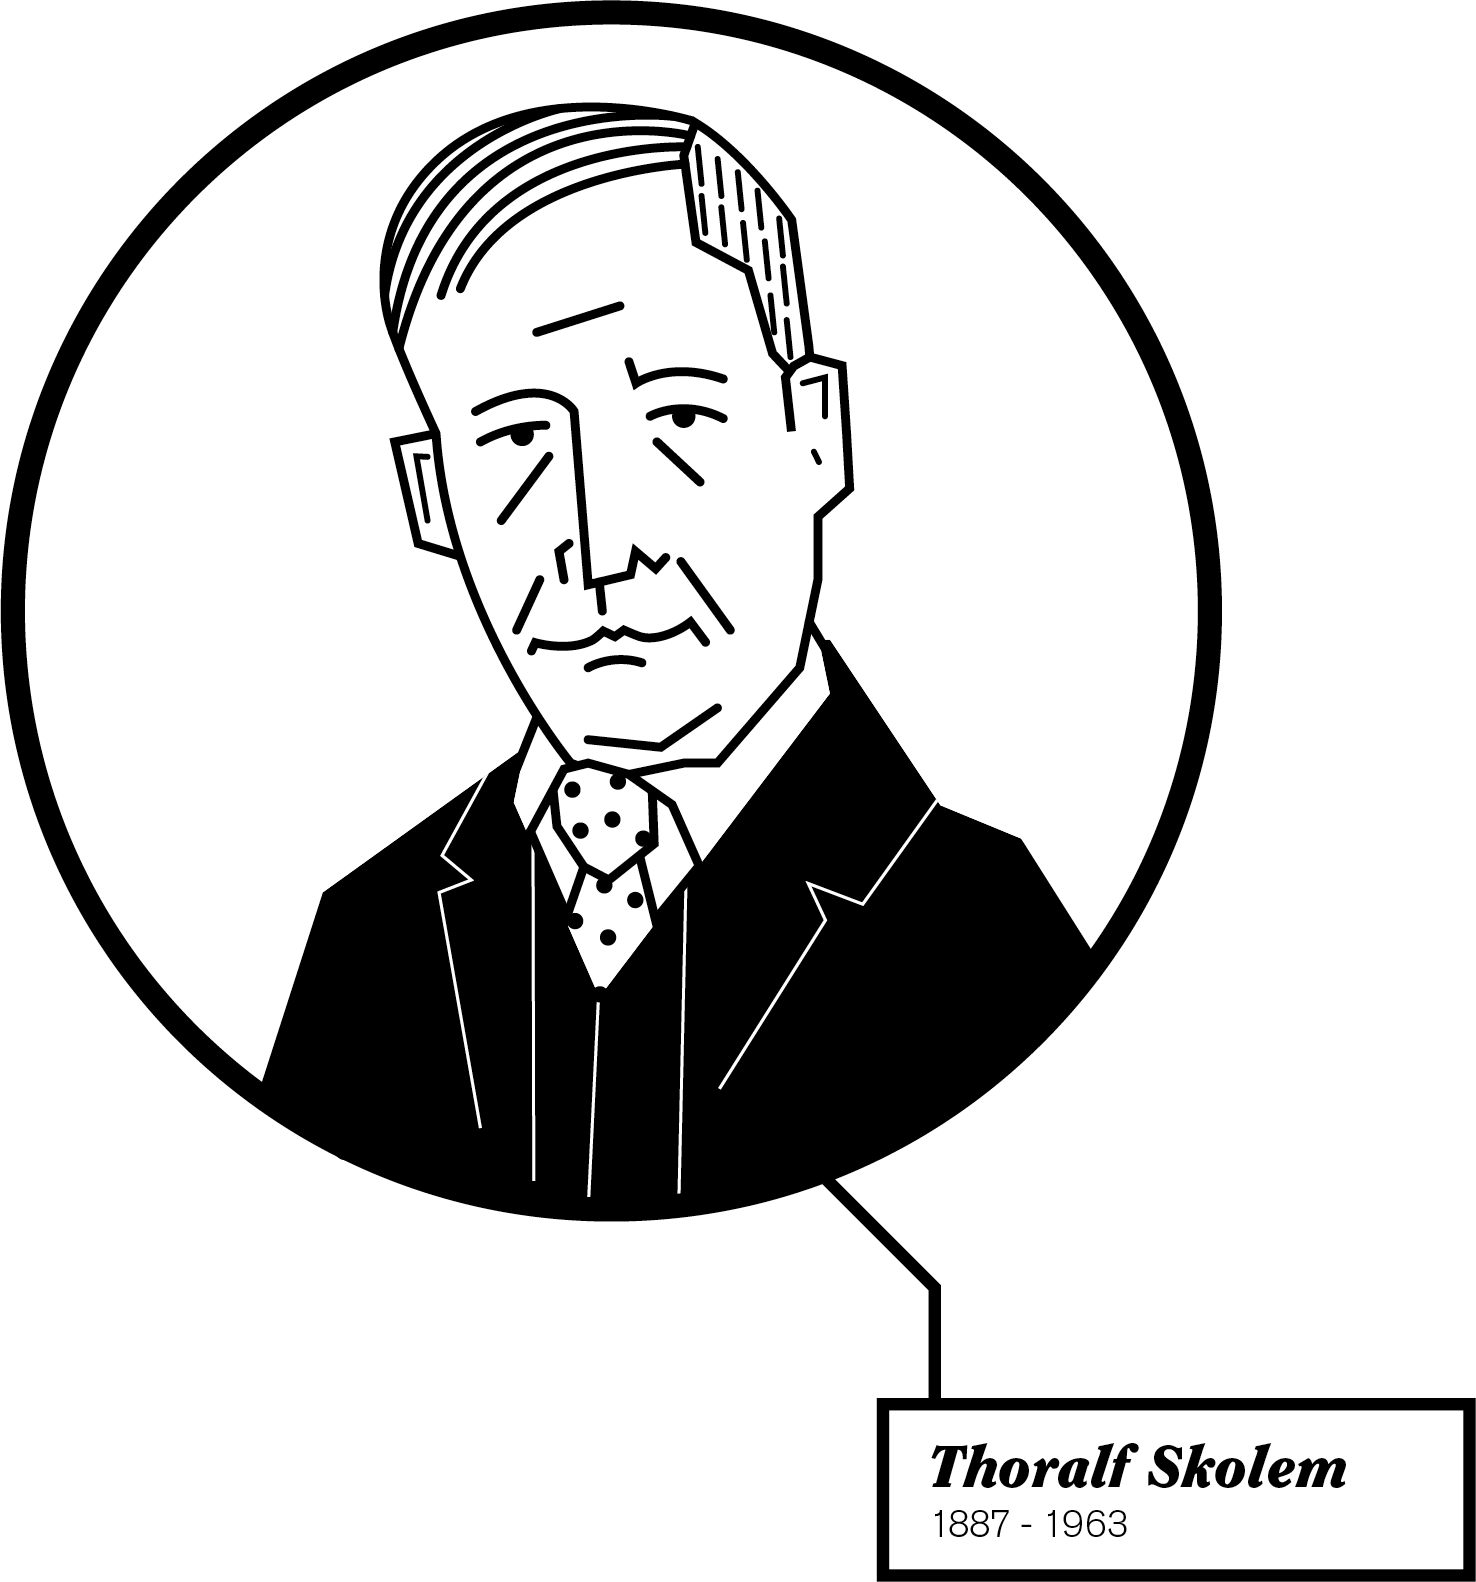
\includegraphics[width=\textwidth]{illustrations/SkolemChapter}
\vfill

\chapter{प्रस्तावना}

हे पुस्तक अधितर्कशास्त्राचा परिचय करून देते. ते विशेषतः संगणकशास्त्र आणि तत्त्वज्ञान यांच्या विद्यार्थ्यांसाठी आहे. तर्कशास्त्राचाच अभ्यास करणारी शाखा असल्यामुळे तिला ``अधितर्कशास्त्र'' असे नाव आहे. तर्कशास्त्रात वैध अनुमानाच्या नियमांचा विचार केला जातो. तर्कशास्त्राचे चिन्हात्मक किंवा आकारिक रूप हे नियम विधानीय किंवा प्रथम-क्रम तर्कशास्त्राच्या भाषांसारख्या आकारिक भाषांत मांडते. अधितर्कशास्त्रात या भाषांचे आणि त्या वापरून केलेल्या योग्य अनुमानाच्या नियमांचे गुणधर्म तपासले जातात. या आकारिक भाषांतील अभिव्यक्तींना नेमका अर्थ कसा द्यावा, वैध अनुमानाच्या नियमांचे समर्थन कसे करावे आणि विविध !!{derivation} पद्धतींचे गुणधर्म, त्यांच्या संगणनविषयक गुणधर्मांसह, कोणते आहेत, अशा प्रश्नांचा त्यात विचार होतो. येथे तपासलेल्या भाषा आणि !!{derivation} पद्धती अनेक क्षेत्रांत, विशेषतः गणित, तत्त्वज्ञान, संगणकशास्त्र आणि भाषाविज्ञान यांत वापरल्या जातात. त्यामुळे हे प्रश्न स्वतःच महत्त्वाचे आणि रंजक आहेत. शिवाय, सर्वसाधारणपणे आकारिक प्रणाल्यांचा अभ्यास कसा करावा हेही त्यांतून दिसते. येथे आपण ज्या तार्किक भाषा अभ्यासतो त्यांखेरीज इतरही भाषा अभ्यासकांच्या दृष्टीने महत्त्वाच्या आहेत. उदाहरणार्थ, भाषावैज्ञानिक आणि तत्त्वज्ञ यांना विधानीय व प्रथम-क्रम तर्कशास्त्राच्या भाषांपेक्षा कितीतरी गुंतागुंतीच्या भाषांत रस असतो. संगणकशास्त्रज्ञांना तर प्रोग्रामिंग भाषांसारख्या वेगळ्याच \emph{प्रकारच्या} भाषांत रस असतो. आकारिक भाषांची चिन्हार्थमीमांसा कशी द्यावी, त्यांच्याविषयीचे निष्कर्ष कसे सिद्ध करावेत आणि त्यांचे गुणधर्म कसे तपासावेत, यासाठी आपण पाहणार असलेल्या पद्धती तिथेही लागू होतात.

इतर कोणत्याही विद्याशाखेप्रमाणे अधितर्कशास्त्रातही निष्कर्ष किंवा तथ्ये आहेत आणि पद्धती व तंत्रेही आहेत. या पुस्तकात दोन्हींचा विचार केला आहे. पुष्कळ विद्यार्थ्यांना हा अभ्यासक्रम संपल्यावर आपण पाहिलेल्या प्रत्येक निष्कर्षाची गरज पडणार नाही, पण ते निष्कर्ष प्रस्थापित करण्यासाठी आपण ज्या पद्धती वापरतो त्यांची त्यांना गरज पडेल आणि ते त्या वापरतील. उदाहरणार्थ, लोव्हेनहाइम--स्कोलेम प्रमेय संगणकशास्त्रात वारंवार वापरले जात नाही, पण त्याच्या सिद्धतेसाठी आपण वापरतो त्या पद्धती तिथे वापरल्या जातात. याउलट, आपण पाहणार असलेले अनेक निष्कर्ष विज्ञानाचे तत्त्वज्ञान आणि सत्तामीमांसा यांतील काही वादांना लागू पडतात. तत्त्वज्ञानाच्या विद्यार्थ्यांना अभ्यासक्रमाबाहेर हे निष्कर्ष सिद्ध करता येण्याची गरज भासेलच असे नाही, पण त्यांचा आशय समजला पाहिजे. ते प्रस्थापित करण्यासाठी लागणाऱ्या व्याख्यांचा आणि सिद्धतांचा नीट विचार केला तरच हे निष्कर्ष खऱ्या अर्थाने \emph{समजतात}. या पुस्तकातील निष्कर्ष आणि पद्धती यांचा अभ्यास संगणकशास्त्र व तत्त्वज्ञान यांच्या विद्यार्थ्यांना सुचवला जातो, आणि काही अभ्यासक्रमांत तो आवश्यकही असतो, याची ही काही कारणे आहेत.

पुस्तकाचे तीन भाग आहेत. \Olref[sfr][][]{part} संचसिद्धान्ताविषयी आहे. तर्कशास्त्र व अधितर्कशास्त्र यांचा ``गणिताची पायाभरणी'' असे ज्याला म्हणतात त्याच्याशी ऐतिहासिकदृष्ट्या निकटचा संबंध आहे. पूर्णांक, परिमेय व वास्तव संख्या, फलने, अवकाश इत्यादी गणितीय वस्तू मुळात कशा समजून घ्याव्यात हा त्या अभ्यासाचा विषय आहे. संचसिद्धान्त त्याचे एक उत्तर देतो (इतरही उत्तरे आहेत). म्हणूनच संचसिद्धान्त आणि तर्कशास्त्र यांचा दीर्घकाळ एकत्र अभ्यास होत आला आहे. कोणत्याही प्रकारच्या आकारिक अभ्यासात संच, संबंध आणि फलने सर्वत्र आढळतात. गणिताबरोबरच संगणकशास्त्रात आणि तत्त्वज्ञानाच्या काही अधिक तांत्रिक शाखांतही ती दिसतात. तर्कशास्त्राची चिन्हार्थमीमांसा, सिद्धता उपपत्ती आणि संगणनक्षमतेची पायाभूत तत्त्वे यांविषयी निष्कर्ष मांडण्यासाठी व सिद्ध करण्यासाठी योग्य परिभाषा असणे आवश्यक आहे. उदाहरणार्थ, आपण अभिव्यक्तींचे संच, तार्किक निष्पन्नतेचे व सिद्धतायोग्यतेचे संबंध, विधेयचिन्हांचे अर्थनिर्धारण (त्यातून संबंधच मिळतात), संगणनक्षम फलने, त्यांच्यातील विविध संबंध आणि त्यांचा वापर करून केलेल्या विविध रचना यांविषयी बोलू. यासाठी संक्षिप्त संकेत असणे आणि संच, संबंध व फलने यांच्या सर्वसाधारण गुणधर्मांचा विचार करणे सोयीचे ठरेल. गणितीय विचार करण्याची आणि गणितीय सिद्धता मांडण्याची सवय नसेल, तर संचसिद्धान्ताचा पहिला भाग सरावाची संधी समजा. सर्व मूलभूत व्याख्या दिल्या जातील आणि त्यांचा वापर करून क्रमाक्रमाने अधिक गुंतागुंतीच्या सिद्धता दिल्या जातील. विशेषतः पहिल्या भागात, या सिद्धता समजून घेणे आणि त्या स्वतः शोधून मांडता येणे हे बहुधा निष्कर्ष समजून घेण्यापेक्षा अधिक महत्त्वाचे आहे. गणितीय विचार करण्याची तुम्हाला सवय नसेल, तर उदाहरणांचा आणि समस्यांचा नीट विचार करणे महत्त्वाचे आहे.

पहिल्या भागात मात्र आपण एक महत्त्वाचा निष्कर्ष प्रस्थापित करू. हा निष्कर्ष म्हणजे कँटरचे प्रमेय. विज्ञानात संकल्पनाविश्लेषणाची जी अत्यंत उल्लेखनीय उदाहरणे आढळतात त्यांपैकी एका उदाहरणावर तो आधारलेला आहे. ते म्हणजे कँटर यांनी केलेले अनंततेचे विश्लेषण. अनेक शतके गणितज्ञ आणि तत्त्वज्ञ दोघांनाही अनंततेने कोड्यात टाकले आहे. कँटर यांच्यापूर्वी तिचा नेमका विचार कसा करावा हे कोणालाच ठाऊक नव्हते. तिचा विचार करणे हीच चूक आहे आणि अनंत संग्रह ही कल्पनाच विसंगत आहे असेही पुष्कळांना वाटत असे. कँटर यांनी अनंततेचा सुसंगतपणे अभ्यास करणे शक्य केले. त्यांनी अनंत संग्रहांची आणि त्या संग्रहांचे आकारमान मोजता येईल अशा अनंत संख्यांची संपूर्ण उपपत्ती विकसित केली. अनंततेच्या वेगवेगळ्या पातळ्या आहेत हे त्यांनी दाखवले. ``अनंतपार'' संख्यांची ही उपपत्ती सुंदर आणि गुंतागुंतीची आहे. आपण तिच्यात फार खोलवर जाणार नाही, पण अनंततेच्या वेगवेगळ्या पातळ्या आहेत, विशेषतः ``गणनीय'' आणि ``अगणनीय'' पातळ्या आहेत, हे दाखवू शकू. या निष्कर्षाचे महत्त्वाचे उपयोग आहेत. शिवाय आपल्या विषयाची जाण ठेवू इच्छिणाऱ्या प्रत्येक गणितज्ञाला, संगणकशास्त्रज्ञाला आणि तत्त्वज्ञाला माहीत असावा असा हा निष्कर्ष आहे.

\olref[fol][][]{part} मध्ये आपण प्रथम-क्रम तर्कशास्त्राकडे वळतो. आपण प्रथम-क्रम तर्कशास्त्राची भाषा आणि तिची चिन्हार्थमीमांसा यांची व्याख्या करू. म्हणजेच प्रथम-क्रम रचना म्हणजे काय आणि प्रथम-क्रम तर्कशास्त्राचे वाक्य एखाद्या रचनेत केव्हा सत्य ठरते हे ठरवू. यामुळे आपल्याला दोन महत्त्वाच्या गोष्टी करता येतील. (1)~एखादे वाक्य दुसऱ्या वाक्यापासून तार्किकरीत्या केव्हा निष्पन्न होते हे गणितीय काटेकोरपणे सांगता येईल. (2)~प्रथम-क्रम रचनेतील संबंधांचे वर्णन, म्हणजेच त्यांचे लक्षणचित्रण, त्या रचनांमध्ये सत्य असणारी वाक्ये कशा रीतीने करतात हे पाहता येईल. यातून विशेषतः स्वयंसिद्धकीय पद्धतीची चर्चा पुढे येते. या पद्धतीत विशिष्ट प्रकारच्या रचनांचे लक्षणचित्रण करण्यासाठी प्रथम-क्रम भाषांतील वाक्ये वापरली जातात. पुढे आपण सिद्धता उपपत्ती पाहू. त्यात गरहार्ड गेंटझेन यांनी १९३० च्या दशकात परिभाषित केलेली क्रमवर्ती कलनाची आणि नैसर्गिक निगमनाची मूळ रूपे पाहू. (तुमचे अध्यापक यांपैकी एकच पद्धत शिकवण्याचे ठरवू शकतात. तसे झाल्यास ``!!{derivation}s'' आणि ``!!{derivability}'' यांचा उल्लेख त्यांनी निवडलेल्या पद्धतीच्या संदर्भात समजावा.) एखादे वाक्य इतर काही वाक्यांवरून निष्पन्न होते ही कल्पना नेमकी करण्याचे दोन सर्वस्वी वेगळे मार्ग आपल्याला मिळतात. एक म्हणजे तार्किक निष्पन्नतेची चिन्हार्थविषयक संकल्पना आणि दुसरा म्हणजे !!{derivability} ची विन्यासात्मक संकल्पना. निर्दोषता आणि संपूर्णता ही प्रमेये या दोन लक्षणचित्रणांचा संबंध जोडतात. विशेषतः आपण गोडेल यांचे संपूर्णता प्रमेय सिद्ध करू. त्यानुसार एखादे वाक्य इतर काही वाक्यांपासून चिन्हार्थाच्या दृष्टीने निष्पन्न होत असेल, तर ते त्यांच्यापासून !!{derivable} ही असते. याची समतुल्य मांडणी अशी आहे. एखादा वाक्यसंच सुसंगत असेल, म्हणजे त्यावरून व्याघात सिद्ध करता येत नसेल, तर ती सर्व वाक्ये सत्य ठरतील अशी एखादी रचना असते.

संपूर्णता प्रमेयाची दुसरी मांडणी कदाचित अधिक आश्चर्यकारक आहे. गोडेल यांनी हा निष्कर्ष सिद्ध केला त्या सुमारास (१९२९ मध्ये) डाव्हीट हिल्बर्ट या जर्मन गणितज्ञाचे एक प्रसिद्ध मत असे होते की गणितीय अस्तित्वासाठी सुसंगतता, म्हणजे व्याघाताचा अभाव, एवढीच अट पुरेशी आहे. दुसऱ्या शब्दांत, एखाद्या रचनेचे किंवा रचनांच्या वर्गाचे सुसंगत वर्णन एखाद्या गणितज्ञाला करता येत असेल, तर अशा रचना अस्तित्वात आहेत असे मानण्याचा त्याला अधिकार असावा. त्या काळात अनेकांना ही कल्पना हास्यास्पद वाटली. एखाद्या रचनेचे वर्णन करताना आपण स्वतःशी विसंगत बोललो नाही, एवढ्यावरून ती रचना खरोखर अस्तित्वात आहे असा निष्कर्ष कसा निघणार? गोडेल यांचे संपूर्णता प्रमेय नेमके हेच सांगते. विरोधापत्तीसारख्या आणि तत्त्वज्ञानाच्या दृष्टीने कुतूहलजनक अशा या पैलूबरोबरच संपूर्णता प्रमेयाचे दोन महत्त्वाचे उपयोगही आहेत. दिलेली वाक्ये सत्य ठरवणाऱ्या रचनांच्या अस्तित्वाविषयी आणखी निष्कर्ष सिद्ध करण्यासाठी ते उपयोगी पडतात. हे निष्कर्ष म्हणजे संहतता प्रमेय आणि लोव्हेनहाइम--स्कोलेम प्रमेय.

\olref[tur][][]{part} मध्ये आपण तर्कशास्त्राचा संबंध संगणनक्षमतेशी जोडतो. यालाही ऐतिहासिक संदर्भ आहे. तर्कशास्त्रातील एखादे दिलेले वाक्य सिद्ध करता येते की नाही हे ठरवणारी यांत्रिक पद्धत शोधणे ही तर्कशास्त्राची एक मूलभूत समस्या म्हणून डाव्हीट हिल्बर्ट यांनी मांडली होती. विधानीय तर्कशास्त्रासाठी अशी पद्धत अर्थातच आहे. सर्व सत्यताकोष्टके तपासली की झाले. ती सांत संख्येने असल्यामुळे या पद्धतीने अखेरीस योग्य उत्तर मिळते. प्रथम-क्रम तर्कशास्त्रासाठी इतकी सरळ पद्धत शक्य नाही, कारण संभाव्य रचना अनंत संख्येने असतात (आणि रचना स्वतःही अनंत असू शकतात). अधिक कल्पक पद्धत शोधण्यासाठी तर्कशास्त्रज्ञ अनेक वर्षे प्रयत्न करत होते. ॲलोन्झो चर्च आणि ॲलन ट्यूरिंग यांनी अखेरीस अशी कोणतीही पद्धत अस्तित्वात नसल्याचे सिद्ध केले. त्यासाठी सर्वसाधारणपणे यांत्रिक पद्धत म्हणजे काय याची प्रथम नेमकी व्याख्या देणे आवश्यक होते. एखादी निर्णयप्रक्रिया सुचवली गेली असती, तर बहुधा ती प्रभावी पद्धत आहे हे ओळखता आले असते. पण कोणतीही प्रभावी पद्धत अस्तित्वात नाही हे सिद्ध करण्यासाठी ``प्रभावी पद्धत'' याची आधी व्याख्या करावी लागते आणि त्या व्याख्येच्या आधारे अशक्यता सिद्ध करावी लागते. ट्यूरिंग यांनी हेच केले. तत्त्वतः एखाद्या यांत्रिक प्रक्रियेला काय करता येते याचे गणितीय प्रतिमान म्हणून त्यांनी ट्यूरिंग यंत्राची\footnote{अर्थात, ट्यूरिंग यांनी स्वतः त्याला हे नाव दिले नव्हते.} कल्पना मांडली. गणितीय साधनांनी एखाद्या अनौपचारिक संकल्पनेचे \emph{संकल्पनाविश्लेषण} करण्याचे हे आणखी एक उदाहरण आहे. कँटर यांचे अनंततेचे विश्लेषण गणिताला जितके महत्त्वाचे आहे, तितकेच हे विश्लेषण संगणकशास्त्राला कदाचित महत्त्वाचे आहे. शेवटचे मोठे काम म्हणजे अशक्यतेची दोन प्रमेये सिद्ध करणे. ``थांबण्याची समस्या'' म्हणून ओळखली जाणारी समस्या ट्यूरिंग यंत्रांना सोडवता येत नाही हे आपण दाखवू. शेवटी, तर्कशास्त्रासाठी हिल्बर्ट यांनी मांडलेली ``निर्णय समस्या''ही त्यांना सोडवता येत नाही हे दाखवू.

हे पुस्तक गणितीय आहे, कारण त्यात आपण गणितीय व्याख्यांची चर्चा करतो आणि आपले निष्कर्ष गणितीय रीतीने सिद्ध करतो. मात्र त्यासाठी गणिताचे विस्तृत पूर्वज्ञान आवश्यक नाही. पुस्तकातील कोणत्याही भागासाठी बीजगणित, त्रिकोणमिती किंवा कलन यांचे ज्ञान लागत नाही. गणितात काम कसे केले जाते याचाही आधीचा परिचय लागणार नाही याची आम्ही विशेष काळजी घेतली आहे. खरे तर, आपले निष्कर्ष समजून घेण्यासाठी आणि सिद्ध करण्यासाठी लागणारे युक्तिविचार आणि सिद्धता देण्याचे कौशल्य \emph{विकसित करणे} हा या पुस्तकाच्या हेतूचा एक भाग आहे. पुस्तकाची मांडणी गणितातील संकेतांनुसार आहे. गणितात स्पष्टता आणि काटेकोरपणा यांना विशेष महत्त्व असल्यामुळे हे संकेत विकसित झाले आहेत. उदाहरणार्थ, एखादी गोष्ट युक्तिवादाचा निष्कर्ष म्हणून मांडली आहे, दुसऱ्या गोष्टीच्या समर्थनार्थ दिली आहे की नव्या संज्ञेची ओळख करून देण्यासाठी आली आहे, हे समजणे आवश्यक असते. म्हणून आपण गणितातील संकेत पाळतो. नवीन संज्ञा किंवा चिन्हे देणाऱ्या मजकुराला ``व्याख्या'' असे म्हणतो आणि निष्कर्ष किंवा एखादी सिद्ध झालेली बाब नोंदवताना ``प्रमेय'', ``विधान'', ``पूर्वप्रमेय'' किंवा ``अनुप्रमेय'' असे म्हणतो. या संकेतांबरोबरच तर्कशास्त्राच्या पहिल्या अभ्यासक्रमातून कदाचित परिचित असलेल्या तार्किक सिद्धतेच्या पद्धती आपण वापरू. निष्कर्ष सिद्ध करण्यासाठी \emph{विगमन} पद्धतीचाही भरपूर वापर करू. परिशिष्टाची दोन प्रकरणे या सिद्धता-पद्धतींना वाहिलेली आहेत.

\paragraph{अध्यापकांसाठी सूचना} या पुस्तकातील सामग्री आकारिक तर्कशास्त्राच्या दुसऱ्या, एका सत्राच्या अभ्यासक्रमासाठी योग्य आहे. कॅलगरी विद्यापीठात मी तर्कशास्त्र~II या अभ्यासक्रमात ती १२ आठवड्यांत शिकवतो. मात्र पुस्तकात दिले आहे तितक्या तपशिलात सर्व विषय शिकवत नाही. उदाहरणार्थ, मी सामान्यतः फक्त नैसर्गिक निगमन शिकवतो आणि एकरूपतेसाठी संपूर्णतेच्या तपशीलवार सिद्धता वगळतो. विद्यार्थ्यांनी त्याआधी तर्कशास्त्र~I हा अभ्यासक्रम घेतलेला असतो. तो सहसा \emph{\href{https://forallx.openlogicproject.org}{forall x: Calgary}} या पुस्तकावरून शिकवला जातो. त्यात नैसर्गिक निगमनाचे हेच नियम वापरले आहेत, पण फिच यांच्या मांडणीत.

या पुस्तकाची सर्वांत अलीकडची PDF आवृत्ती \href{https://slc.openlogicproject.org}{मूळ पाठ्यपुस्तकाच्या संकेतस्थळावर} उपलब्ध आहे, पण ती वारंवार बदलते. CC BY परवान्यामुळे तुम्हाला स्वतः पुस्तक डाउनलोड करून वितरित करण्याचा अधिकार मिळतो.\footnote{CC BY 4.0 हा मजकुराचा परवाना आहे. या मराठी PDF मधील व्यक्तिचित्रे व छायाचित्रे वितरित करताना त्यांच्या स्वतंत्र वापराच्या अटी लागू होतात. त्या पुस्तकाच्या श्रेयपृष्ठांवर दिल्या आहेत.} तुम्ही ते वापरत असलेल्या संपूर्ण सत्रात सर्व विद्यार्थ्यांकडे एकच आवृत्ती असावी यासाठी या अधिकाराचा उपयोग करा. तुम्ही वापरायचे ठरवलेले PDF आपल्या शिक्षण व्यवस्थापन प्रणालीवर अपलोड करा. विद्यार्थ्यांना केवळ दुवा दिल्यास ते एकाच आवृत्तीचा वापर करतील याची खात्री राहत नाही. तुमच्या पुस्तकविक्रेत्याकडून तुम्ही PDF छापून घेऊ शकता. काही पुस्तकविक्रेत्यांना Amazon वर उपलब्ध असलेल्या मऊ मुखपृष्ठाच्या प्रती विकत घेऊन विक्रीसाठी ठेवता येतील.

ग्रॅहम लीच-क्राउस यांचे विनामूल्य ऑनलाइन तर्कशास्त्र अध्यापन साधन \emph{Carnap} (\href{https://carnap.io}{carnap.io}) प्रथम-क्रम तर्कशास्त्राची विन्यासमीमांसा, चिन्हार्थमीमांसा आणि सिद्धता-पद्धती यांच्या अभ्यासाला पूरक आहे. नैसर्गिक निगमन व क्रमवर्ती कलनातील !!{derivation}s, साध्या उपपत्तींसाठी रचना देणे आणि चिन्हांकन यांसारख्या सरावांची उत्तरे त्यात सादर करता येतात आणि त्यांचे स्वयंचलित मूल्यमापन होते. \href{https://turing.openlogicproject.org}{turing.openlogicproject.org} येथे ट्यूरिंग यंत्राचे अनुकरण करणारे साधनही आहे. \olref[tur][][]{part} मधील सामग्री उदाहरणांसह समजावण्यासाठी ते वापरता येते. तिथली उदाहरणे या साधनात आधीच भरलेली आहेत.

\cleartoverso

\thispagestyle{empty}
\ \vfill
\noindent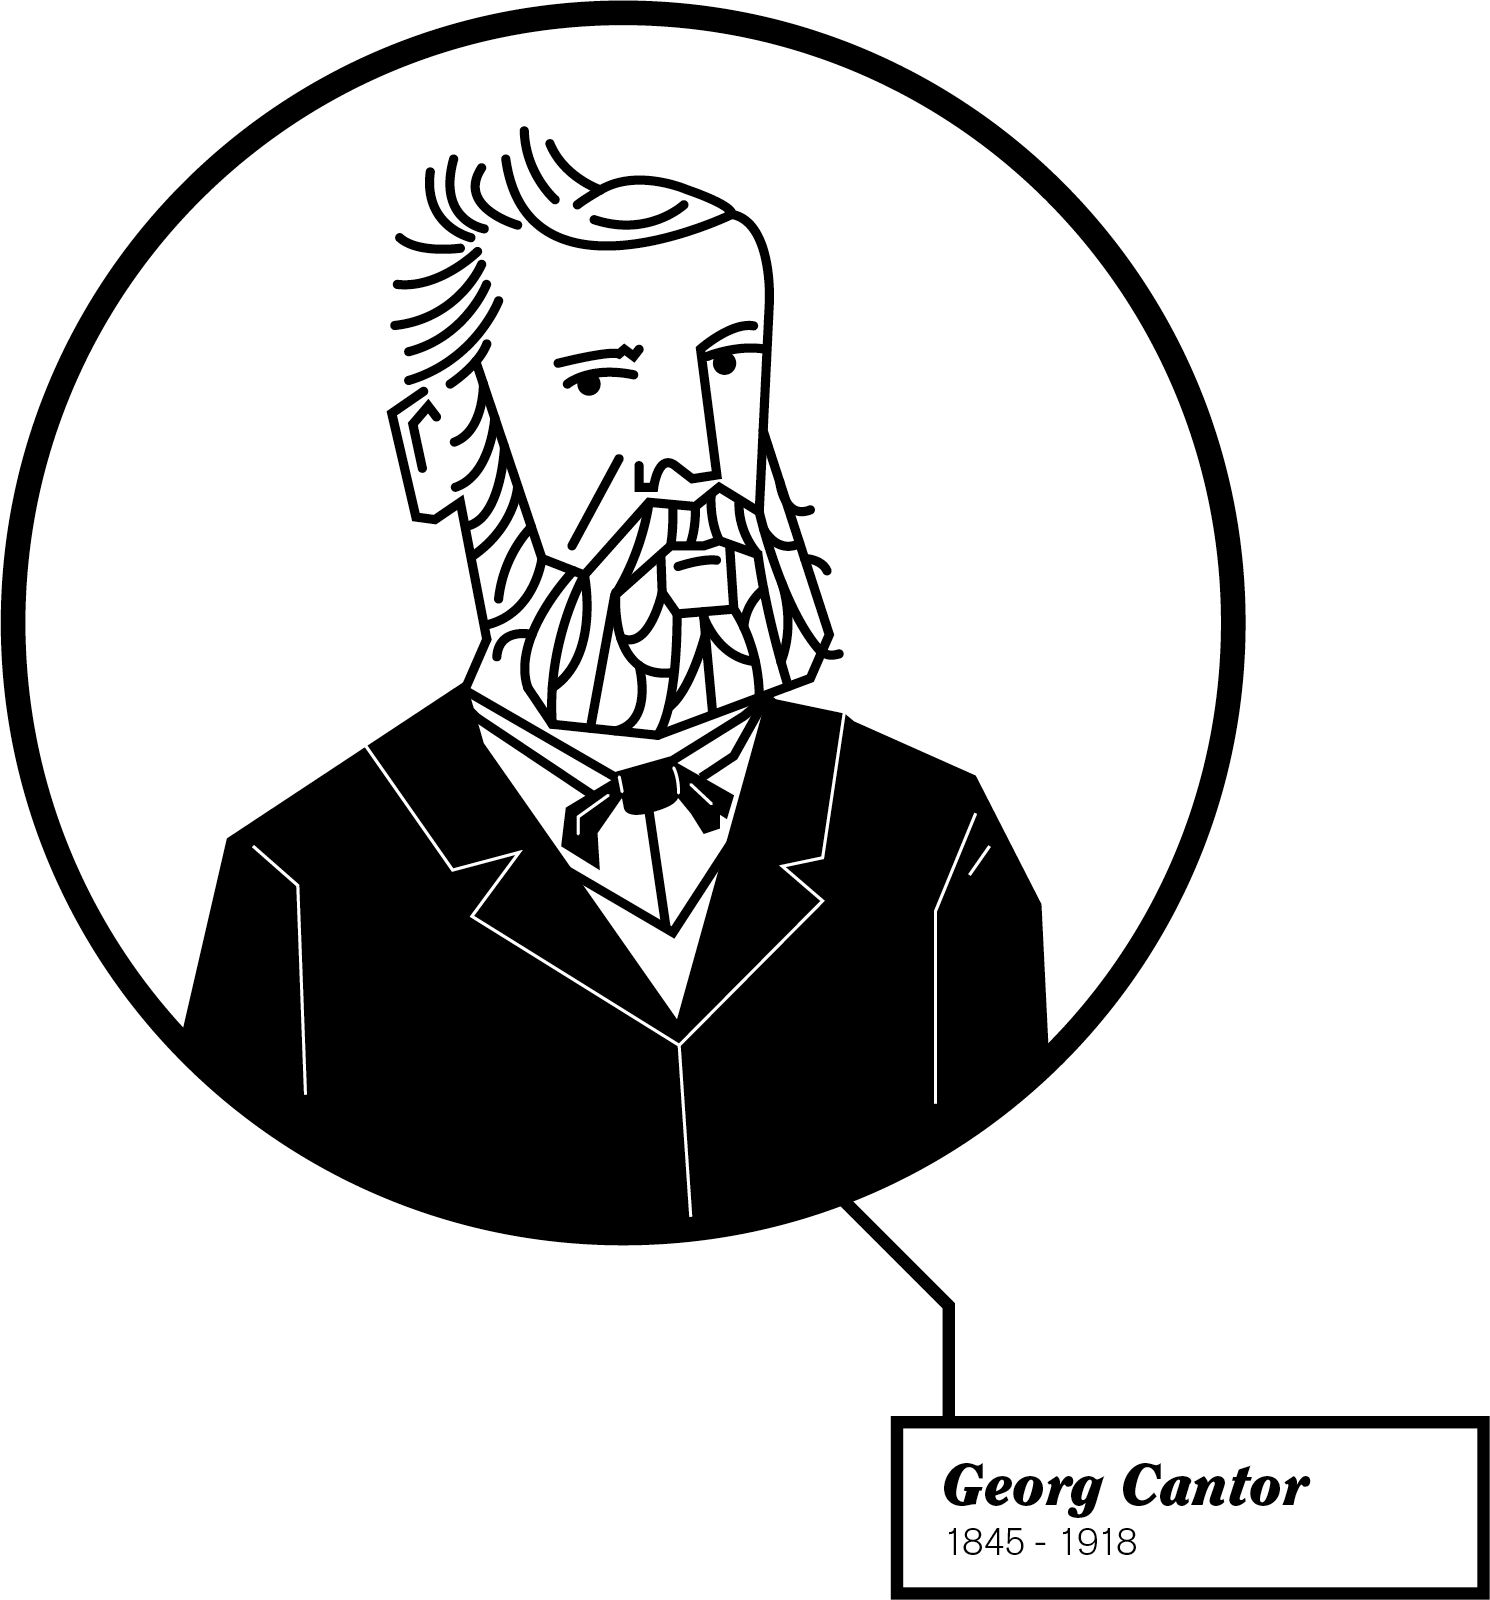
\includegraphics[width=\textwidth]{illustrations/CantorChapter}
\vfill

\mainmatter

\olimport*[sets-functions-relations]{sets-functions-relations}
\cleartoverso
\ifodd\value{page}\stepcounter{page}\fi
\thispagestyle{empty}
\ \vfill
\noindent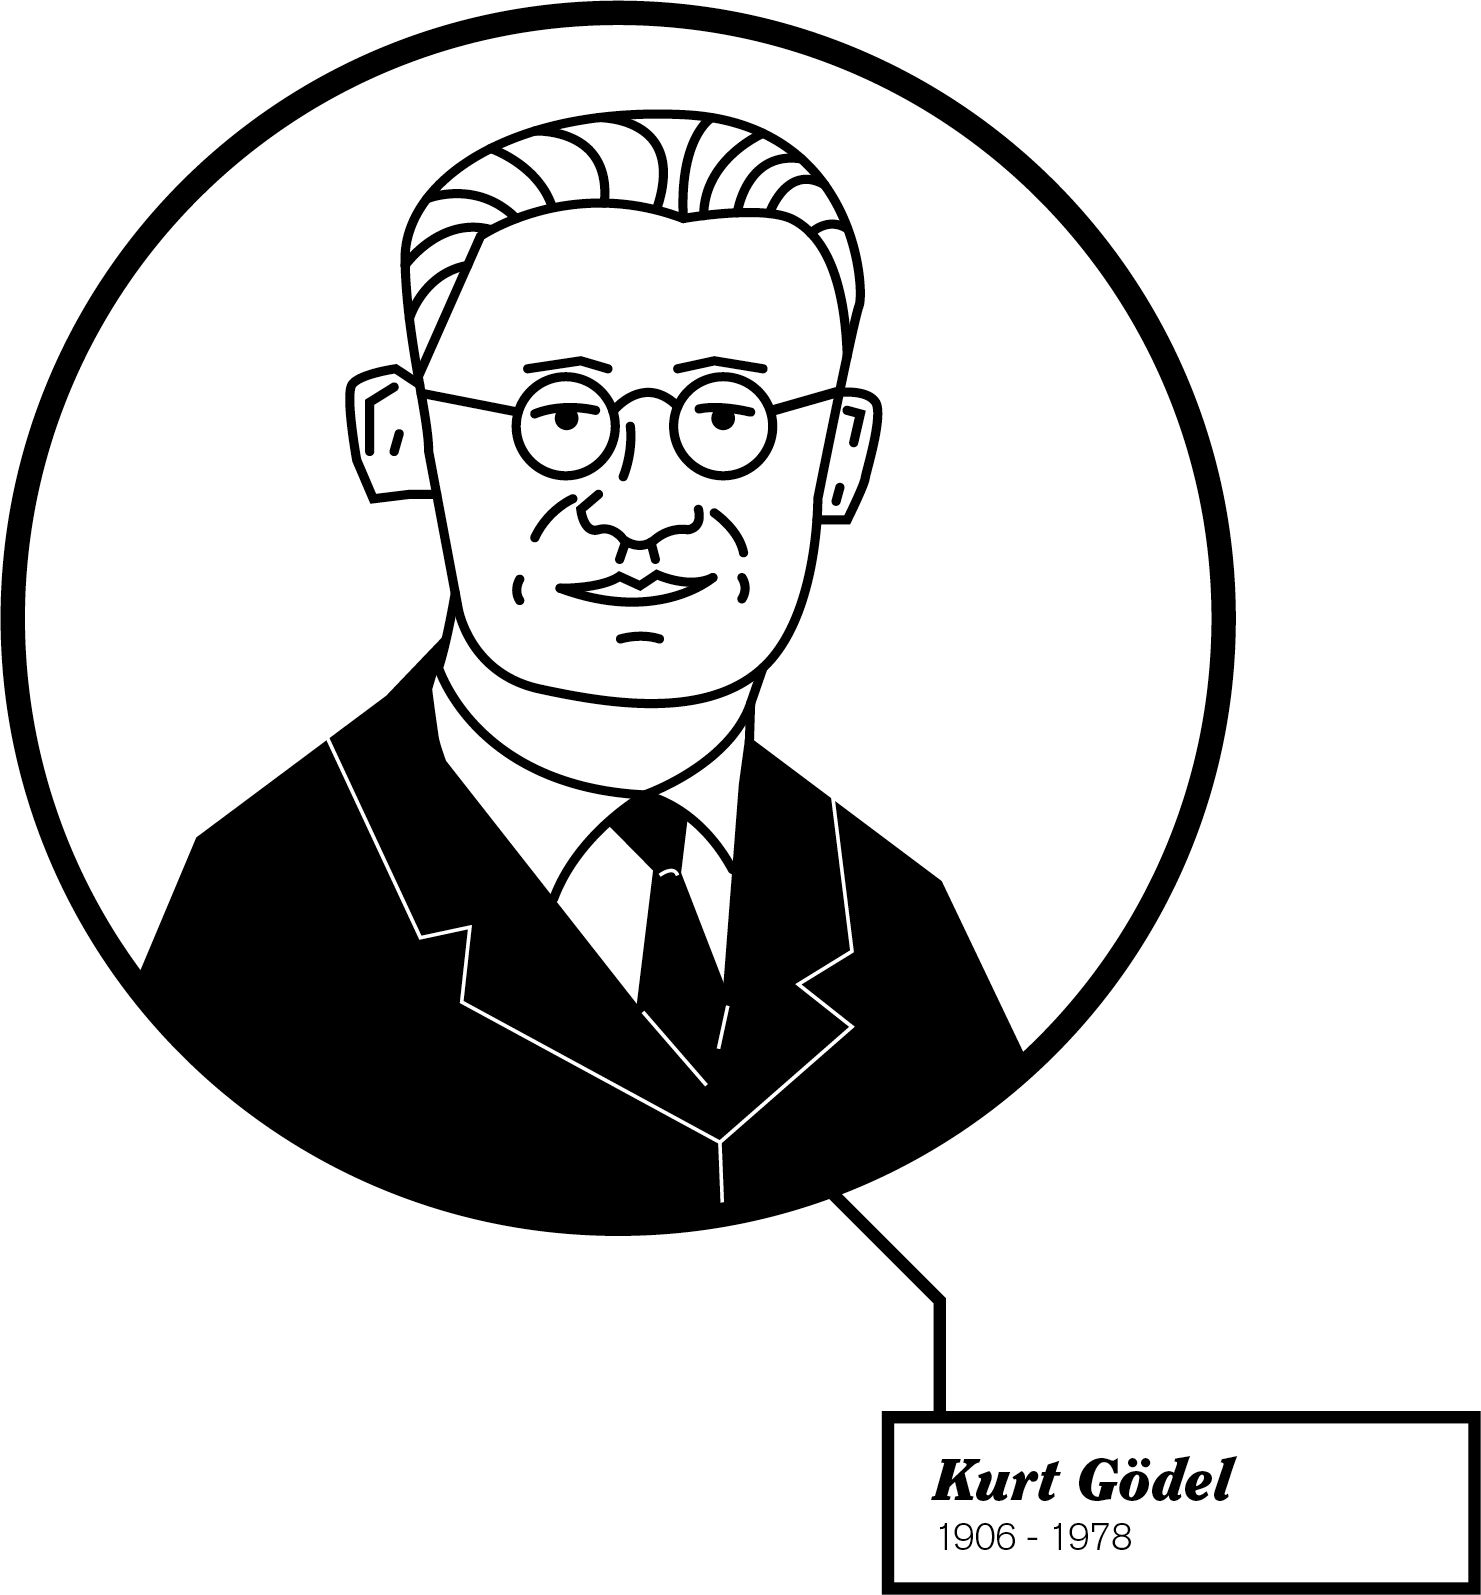
\includegraphics[width=\textwidth]{illustrations/GodelChapter}
\vfill

\olimport*[first-order-logic]{first-order-logic}
\cleartoverso
\ifodd\value{page}\stepcounter{page}\fi
\thispagestyle{empty}
\ \vfill
\noindent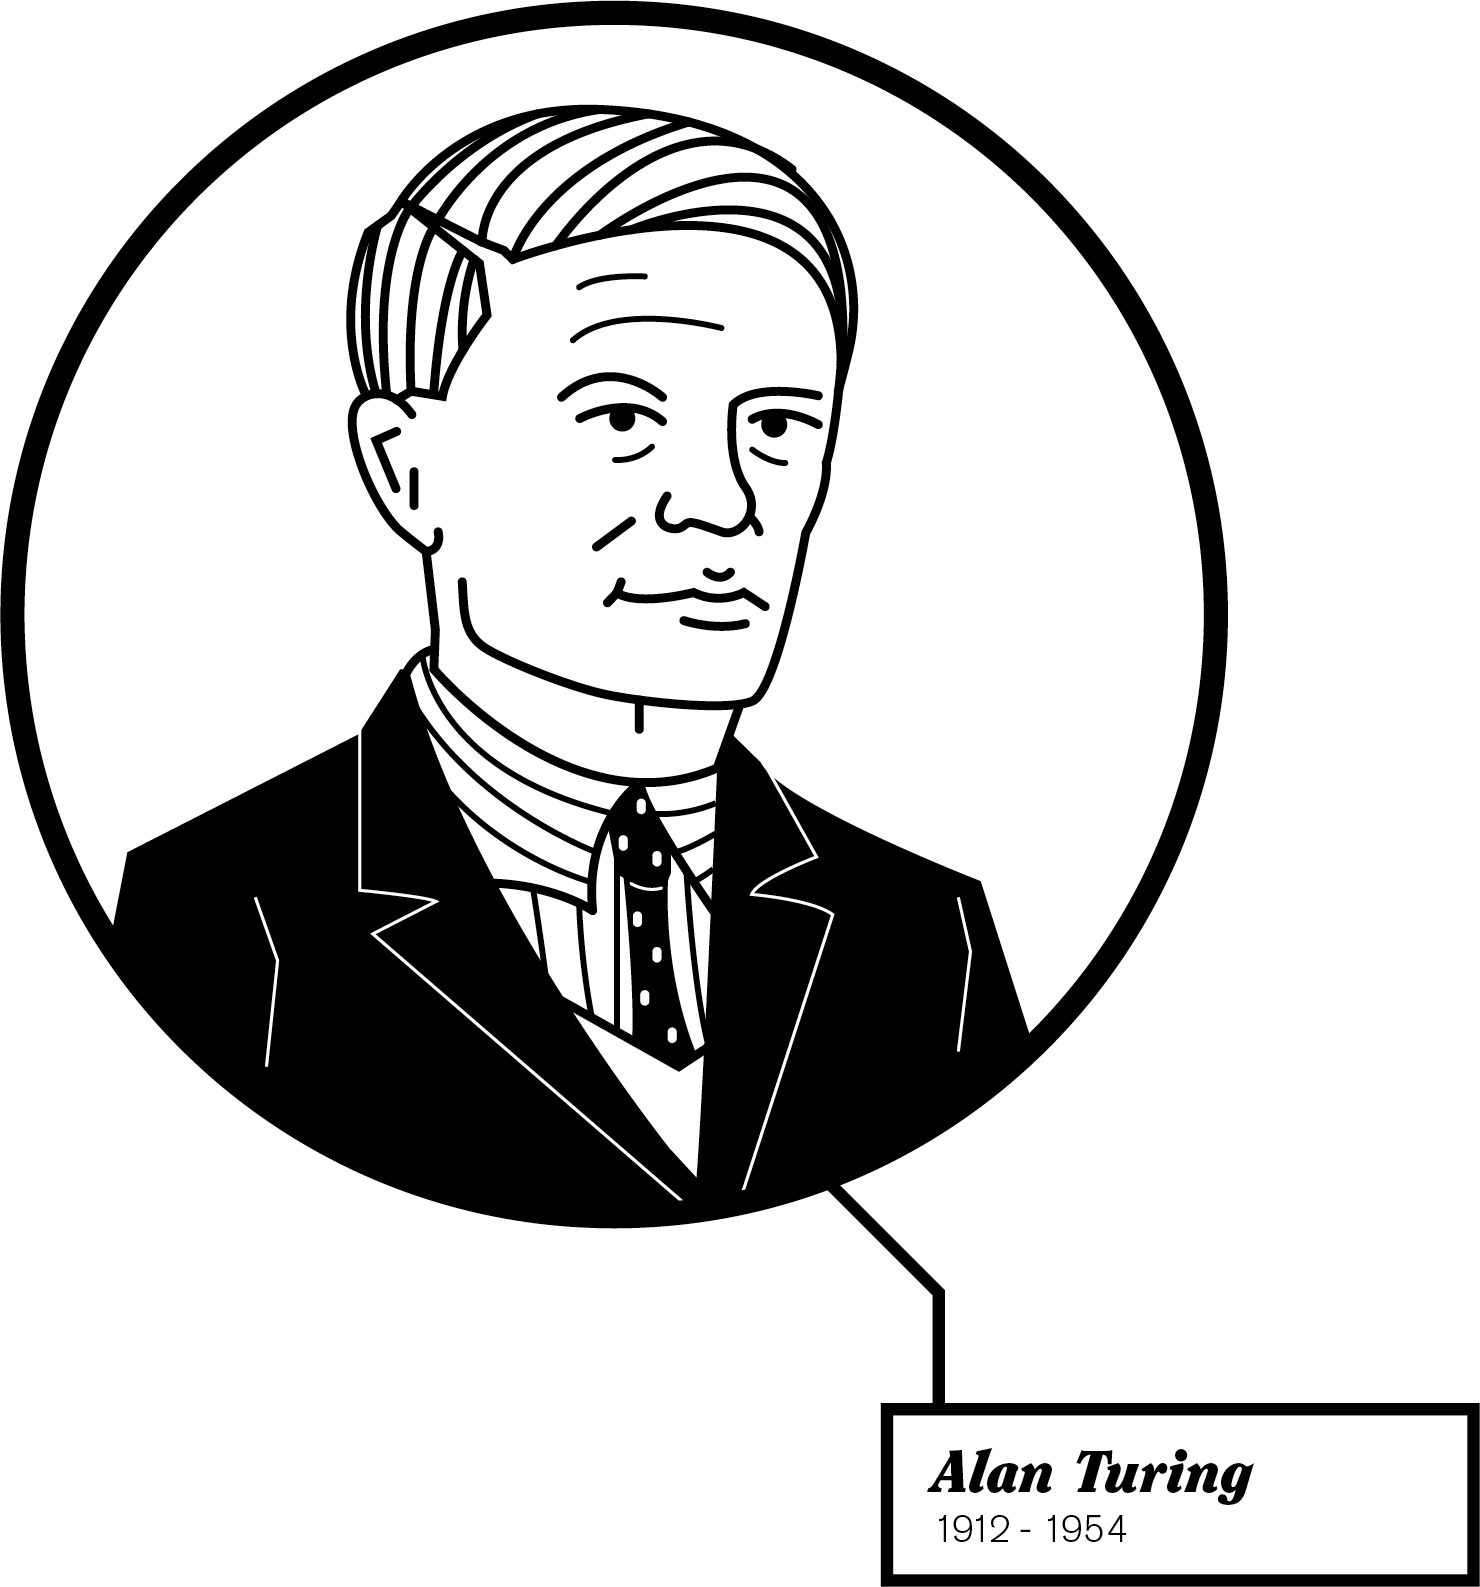
\includegraphics[width=\textwidth]{illustrations/TuringChapter}
\vfill

\olimport*[turing-machines]{turing-machines}

\cleartoverso
\ifodd\value{page}\stepcounter{page}\fi
\thispagestyle{empty}
\ \vfill
\noindent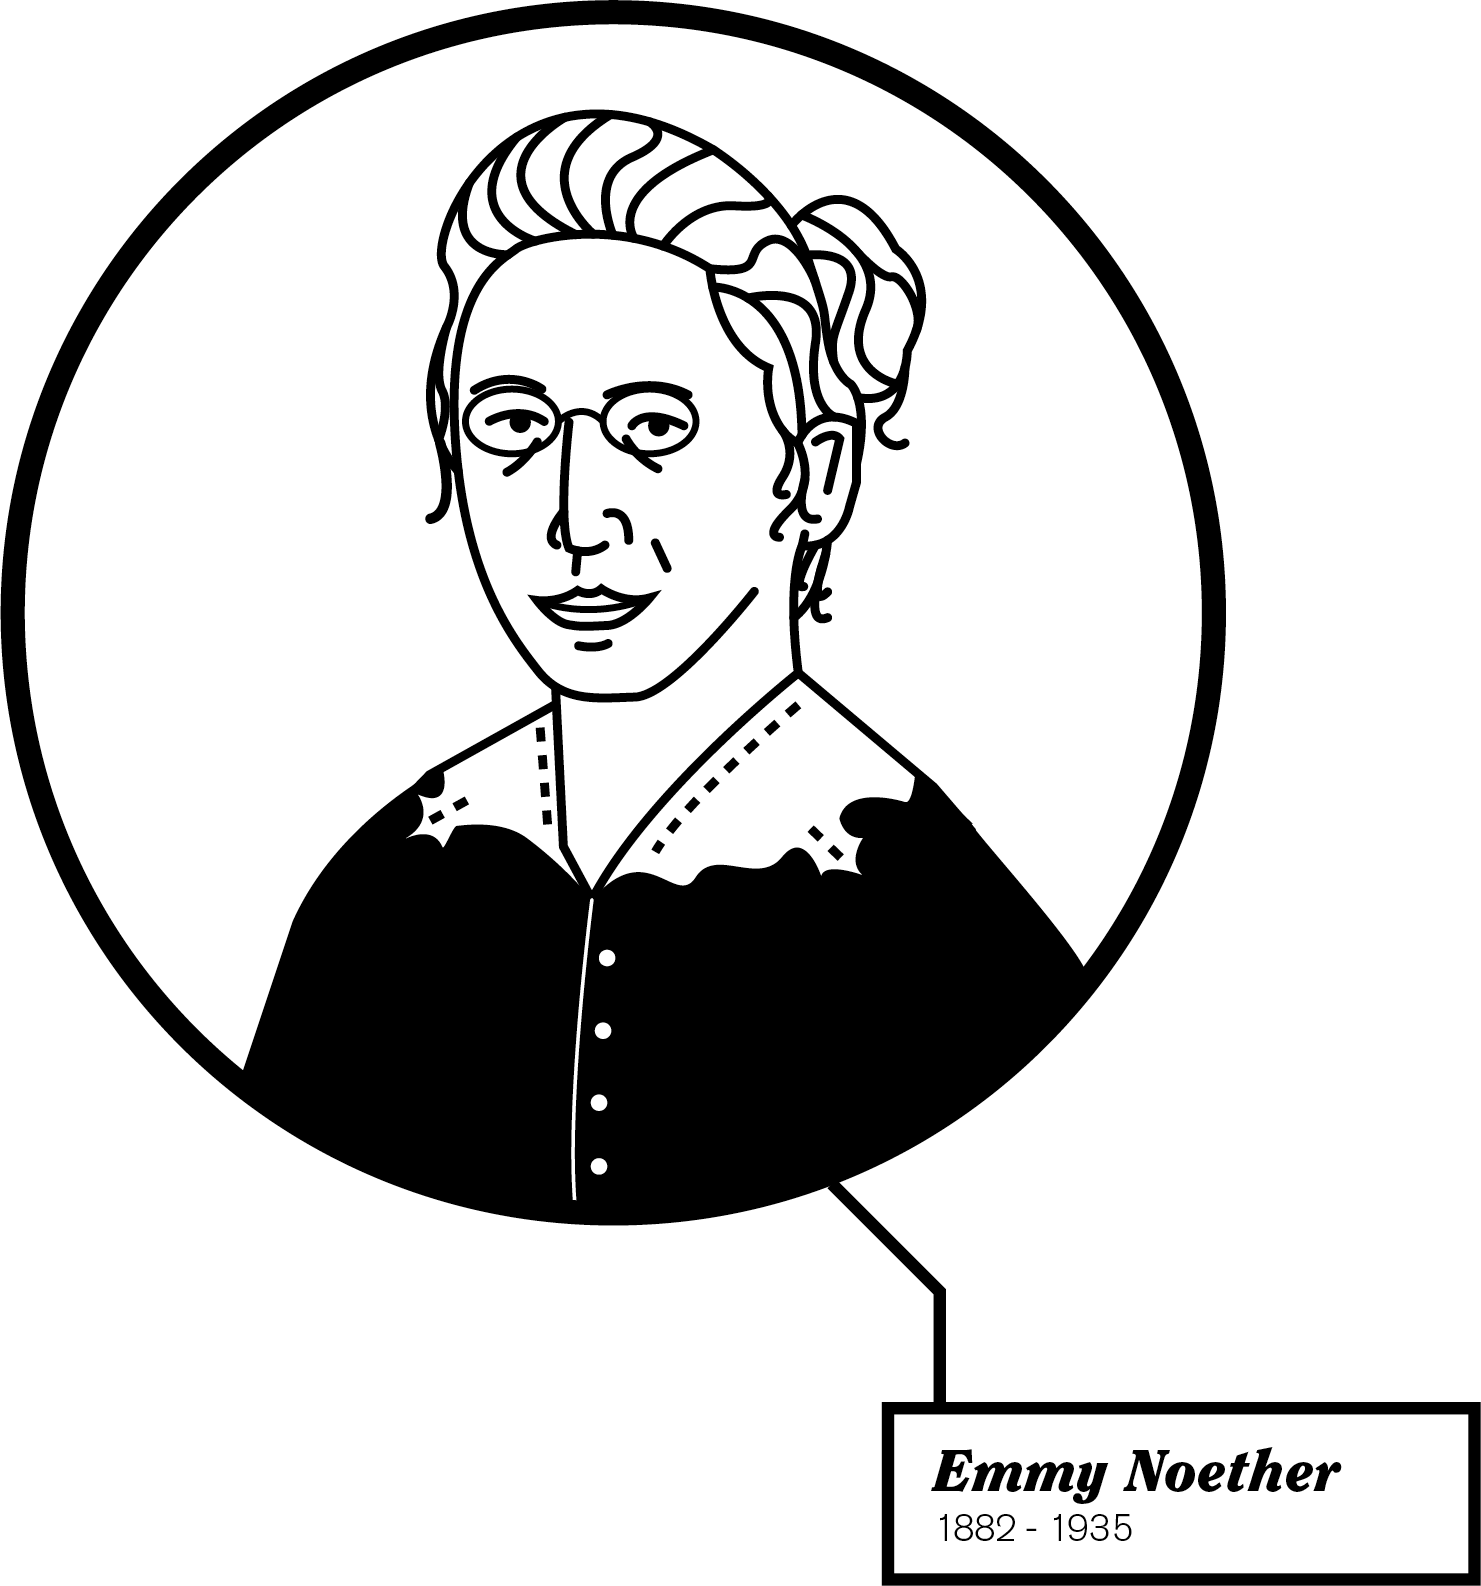
\includegraphics[width=\textwidth]{illustrations/NoetherChapter}
\vfill

% The SLC summary files belong to the numbered chapters.
\slcChapterSummariesfalse
\appendix

\olimport*[methods/proofs]{proofs}

\olimport*[methods/induction]{induction}

\stopproblems
\def\ifproblems#1{}

\setlength{\olphotowidth}{.45\textwidth}

\chapter{चरित्रे}

\olimport*[history/biographies]{georg-cantor}
\olimport*[history/biographies]{alonzo-church}
\olimport*[history/biographies]{gerhard-gentzen}
\olimport*[history/biographies]{kurt-goedel}
\olimport*[history/biographies]{emmy-noether}
\olimport*[history/biographies]{bertrand-russell}
\olimport*[history/biographies]{alfred-tarski}
\olimport*[history/biographies]{alan-turing}
\olimport*[history/biographies]{ernst-zermelo}
\olimport*[reference/greek-alphabet]{greek-alphabet}

\glsaddall
\printglossary[style=index,title=शब्दसूची,toctitle=शब्दसूची]

\clearpage
\photocredits

\bibliographystyle{natbib-oup}
\bibliography{\olpath/bib/open-logic}

{% The two-line Marathi heading leaves less room for the About text.
\addtolength{\beforechapskip}{-\baselineskip}%
\addtolength{\afterchapskip}{-\baselineskip}%
\olimport*{\olpath/locale/\ollangid/content/open-logic-about}\par}

\end{document}
